\documentclass[french]{article}

\usepackage{tikz}
\usepackage{MyPack2}
\geometry{top=2cm, bottom=2cm, left=2cm, right=2cm}
\title{\bsc{SIG} 1}
\author{Binôme A11 \\ \bsc{Simon} Léo, \bsc{Levy--Falk} Hugo}
\date{\today}

\begin{document}
\maketitle

\tableofcontents
\listoffigures
\newpage

\initPage{TL - SIG1}{\today}{\bsc{Simon}, \bsc{Levy--Falk}}

\part{Opérations de base sur les signaux}

\section{Signal numérique de synthèse}

Notre objectif  est de définir quelques fonctions de calcul de base sur les signaux afin de découvrir les outils de Matlab.

\subsection{Génération du signal}

Tout d'abord, nous avons cherché à générer un signal sinusoïdal et à l'échantillonner avant de tracer son graphe. Après avoir effectué quelques tracés, nous avons également pu mettre en évidence le théorème de Niquist-Shannon. La figure \ref{signalSin} montre le résultat obtenu pour une fréquence d'échantillonage de 50 Hz, une fréquence de 4 Hz et N=25.

\begin{figure}[h!]
\centering
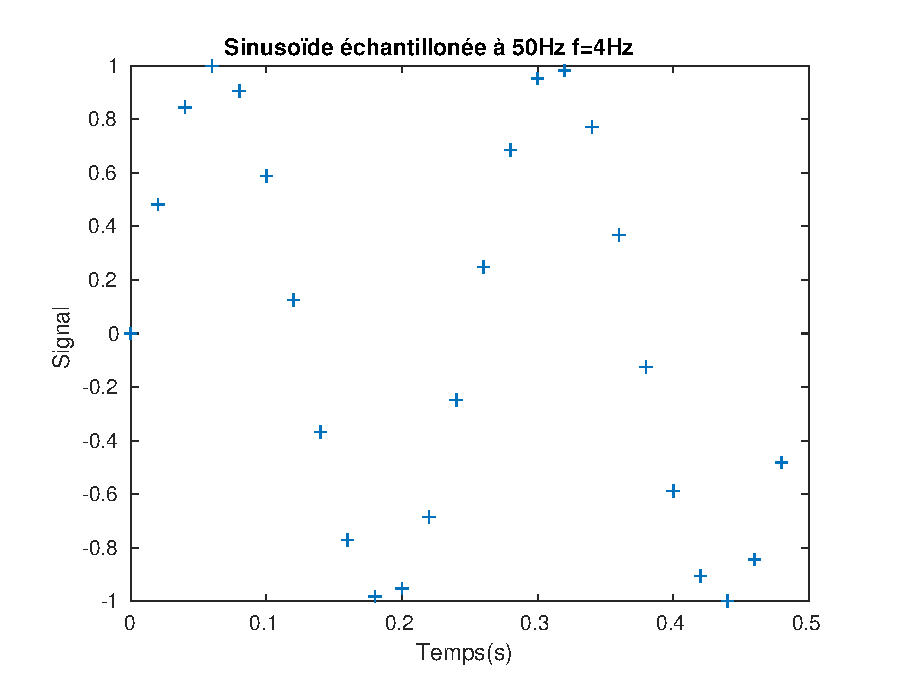
\includegraphics{images/signalSinus.eps}
\caption{Signal sinusoïdal généré.}
\label{signalSin}
\end{figure}

\subsection{ Énergie et puissance}

Dans le but de calculer l'énergie d'un signal sans utiliser \verb`for`, nous avons effectué un produit terme à terme et utilisé l'outil \verb`sum`. Une manière encore plus efficace de procéder aurait été de réaliser le produit entre le vecteur donné en entrée et sa transposée. Nous avons ensuite calculé la puissance moyenne de manière théorique, en utilisant l'identité :

\[
\sin^2(x)=\frac {1-\cos(2x)} {2}
\]

on obtient
\[
\frac{1} {2 \pi} \int_{0}^{2 \pi} \sin^2(x) \mathrm{d}x = 1/2
\]

Par ailleurs, nous avons estimé la puissance de notre signal en utilisant la fonction puissance qui effectue la somme du produit terme à terme du signal et divise par la longueur de ce signal.

\lstset{language=matlab}
\begin{lstlisting}
>> s = sig1_sinus(4, 50, 2*50/4);
>> puissance(s)

ans =

    0.5000
\end{lstlisting}

On obtient un résultat conforme au calcul réalisé.

\subsection{ Quantification}

Pour quantifier un signal sur N bits, on commence par le centrer en 0 et le borner entre -0.5 et 0.5 à l'aide d'une première homothétie. Soit $s_1$ le signal ainsi obtenu. On réalise ensuite la quantification. Si $N > 0$ est le nombre de bit de quantification, on pose $q=\frac{1}{2^N}$. Dans un premier temps, on pose $s_2$ tel que :
\[
  s_2[k] = (\lfloor \frac{s_1[k]}{q} \rfloor + \frac{1}{2}) \times q
\]

Cependant cette formule est problématique pour la valeur maximale atteinte par la fonction. En effet, on a alors :
\[
s_2[k] = ( \lfloor \frac{1}{2q} \rfloor + \frac{1}{2}) \times q ) = (2^{N-1} + \frac{1}{2}) \times \frac{1}{2^N} > \frac{1}{2}
\]

Ce qui est incohérent avec le signal original. Une solution est de poser :
\[
  s_2[k] = min((\lfloor \frac{s_1[k]}{q} \rfloor + \frac{1}{2}) \times q, \frac{1}{2} - \frac{q}{2})
\]

Il ne reste plus qu'à remettre la fonction à l'échelle. On obtient le code suivant :

\lstset{language=matlab}
\begin{lstlisting}
function sig_quant = quantifie(X, n_bit)
    m = min(X);
    M = max(X);
    c = (m+M)/2;
    d = M-m;
    q = 1 / (2 ^ n_bit);
    s1 = (X - c)/d;
    sig_quant = min((floor(s1/q) + 1/2) * q, 1/2-q/2)*d + c;
end
\end{lstlisting}
En appliquant la fonction \verb`quantifie` pour $N=3$ et $N=8$ à un signal généré grâce à la fonction écrite dans la partie 1, on obtient la figure \ref{signalBruit}. On peut noter qu'il est difficile de différencier le signal d'entrée du signal quantifié sur 8 bits. La figure \ref{signalBruit2} montre offre un zoom qui permet de différencier le signal de la quantification.

\begin{figure}[h!]
\centering
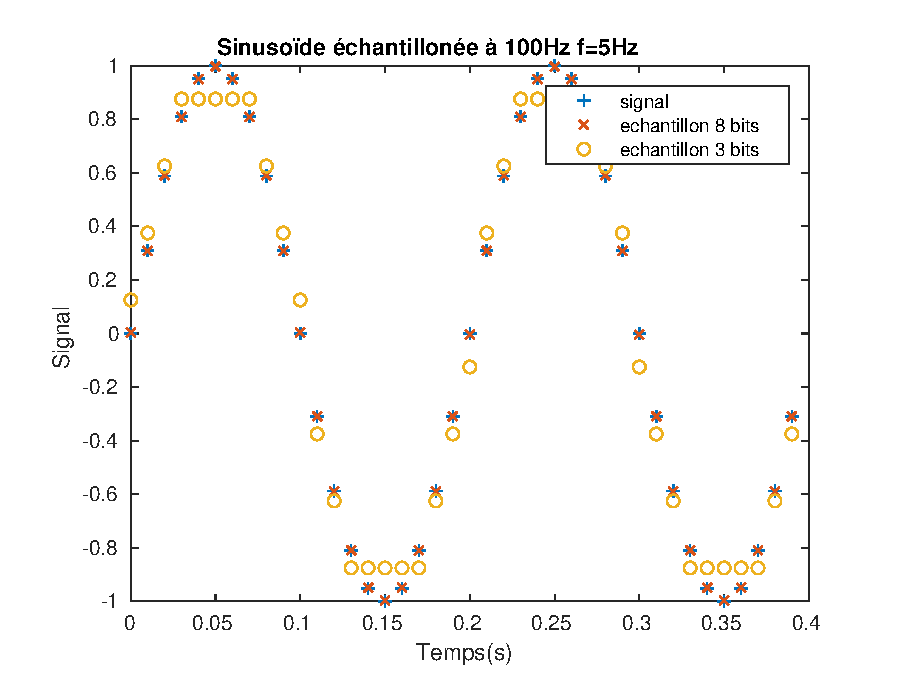
\includegraphics{images/signalBruit.eps}
\caption{Quantification du signal sinusoïdal généré.}
\label{signalBruit}
\end{figure}
\begin{figure}[h!]
	\centering
	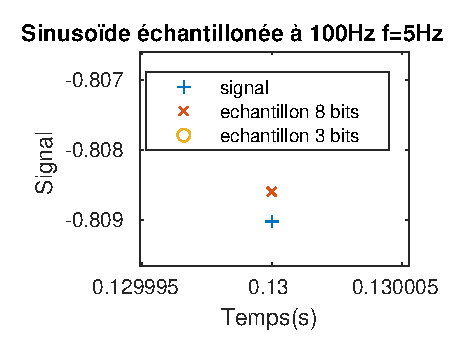
\includegraphics{images/signalBruit1.eps}
	\caption{Quantification du signal sinusoïdal généré - zoom.}
	\label{signalBruit2}
\end{figure}

%\FloatBarrier

Pour déterminer le bruit de quantification, on calcule la différence entre le signal d'origine et le signal quantifié, et on en détermine l'énergie. On calcule également la valeur théorique du bruit de quantification. On obtient

\begin{itemize}
	\item pour 8 bits, $4.6464 \times 10^{-6}$, pour une valeur théorique de $1.272 \times 10^{-6}$;
	\item pour 3 bits, $0.0063$, pour une valeur théorique de $0.0013$.
\end{itemize}
% TODO: SIGNAL SUR BRUIT
On remarque que l'échantillonnage à 8 bits est bien plus efficace, bien que la valeur théorique soit plus faible que celle calculée.

\section{ Signal audio}

\subsection{ Restitution}

En écoutant le signal enregistré à différentes fréquences de restitutions, on remarque que augmenter cette fréquence diminue la durée de la restitution et décale les fréquences de l'enregistrement vers des fréquences plus hautes. Inversement, diminuer la fréquence de restitution augmente la durée de l'enregistrement tout en déplaçant les fréquences des sons de l'enregistrement vers les graves.

\subsection{ Quantification}

A l'aide de la fonction \verb`quantifie` réalisée dans la partie précédente, on réalise la quantification du signal enregistré. On observe que plus le nombre de bits de quantification est faible, plus le bruit (à l'écoute) est important.

Les figures \ref{sonQuantifie1} et \ref{sonQuantifie2} donnent une représentation graphiques de différentes quantification du signal vocal.

\begin{figure}[!h]
\centering
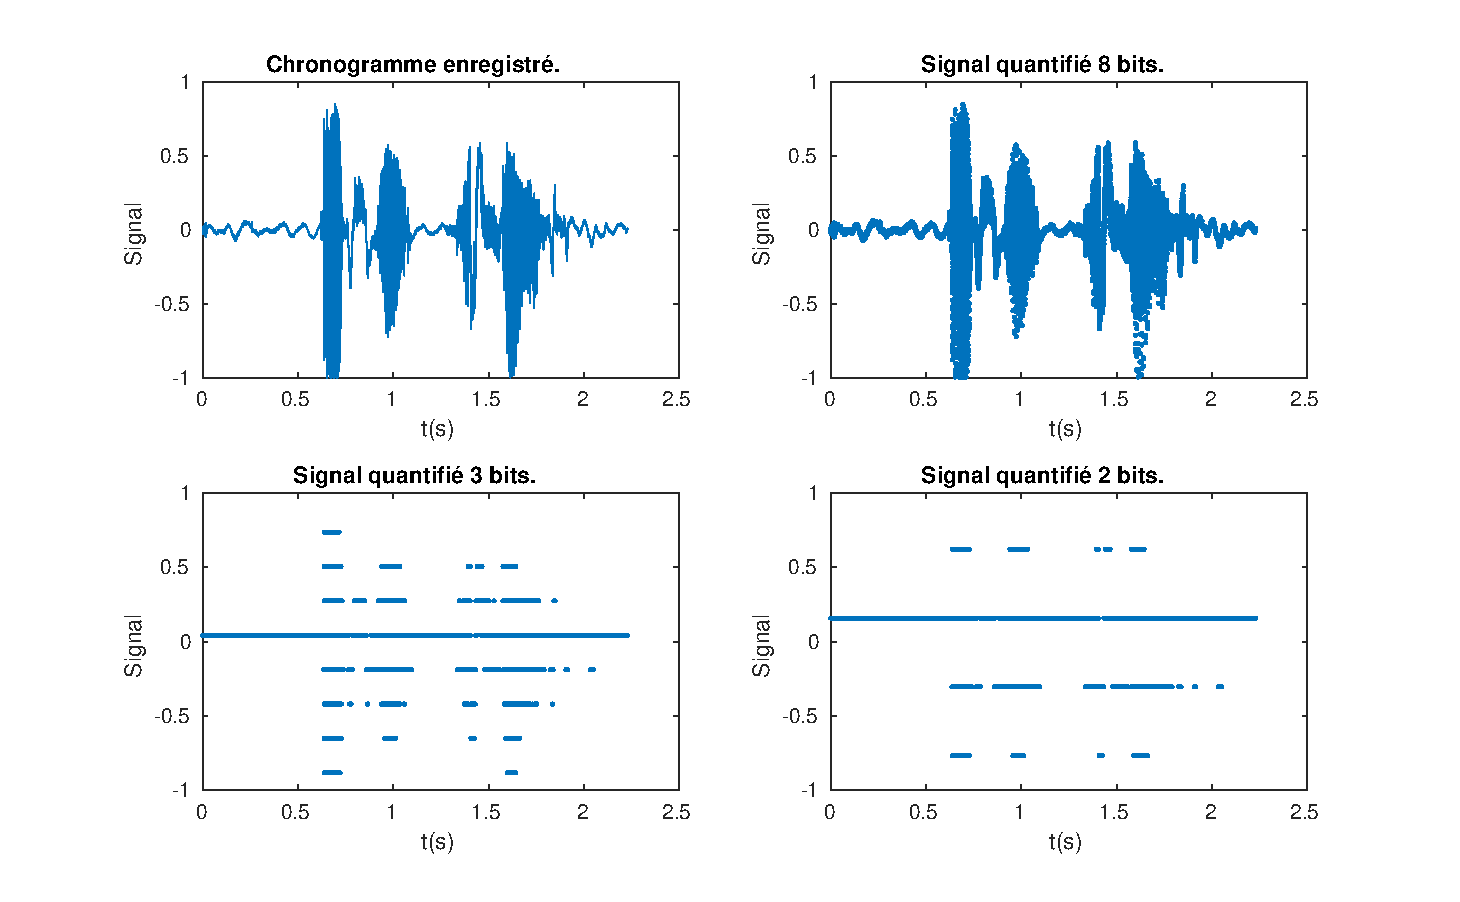
\includegraphics[height=0.45\textheight]{images/sonQuantifie2.eps}
\caption{Quantification du signal vocal enregistré.}
\label{sonQuantifie1}
\end{figure}

\begin{figure}[!h]
\centering
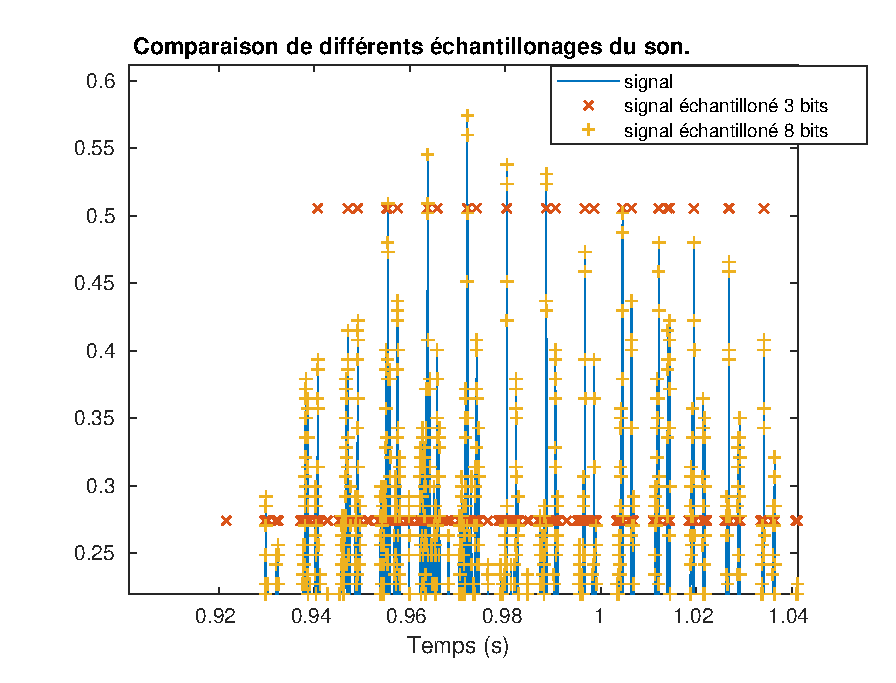
\includegraphics[height=0.45\textheight]{images/sonQuantifie.eps}
\caption{Quantification du signal vocal enregistré - comparaison en zoom.}
\label{sonQuantifie2}
\end{figure}

\FloatBarrier
\newpage
\part{ Classification des signaux}

Le but de cette partie est de classifier les signaux, notamment en utilisant l'autocorrélation.

\section{ Exemple de calcul théorique}

Pour le signal $y(t) = A \sin(2 \pi f t)$, calculons l'autocorrélation :

\[
\gamma_y(\tau) = \int_0^{\frac{1}{f}} A^2 \sin(2\pi f t) \sin(2 \pi f (t+\tau)) dt \
= \frac{A^2}{2} \cos 2\pi f \tau - \frac{A^2}{2}\underbrace{\int_0^{\frac{1}{f}} \cos (2 \pi f (2t + \tau)) dt}_{=0}
\]

On obtient la fonction d'autocorrélation suivante :
\[
\gamma_y (t) = \frac{A^2} {2} cos(2 \pi f t)
\]

\section{ Programmation}

On implémente l'autocorrélation avec la formule suivante :

\[
\gamma_x [n] = \sum_{k = 0} ^{length (x)} x[k]x[k+n]
\]

\begin{figure}[h!]
	\centering
	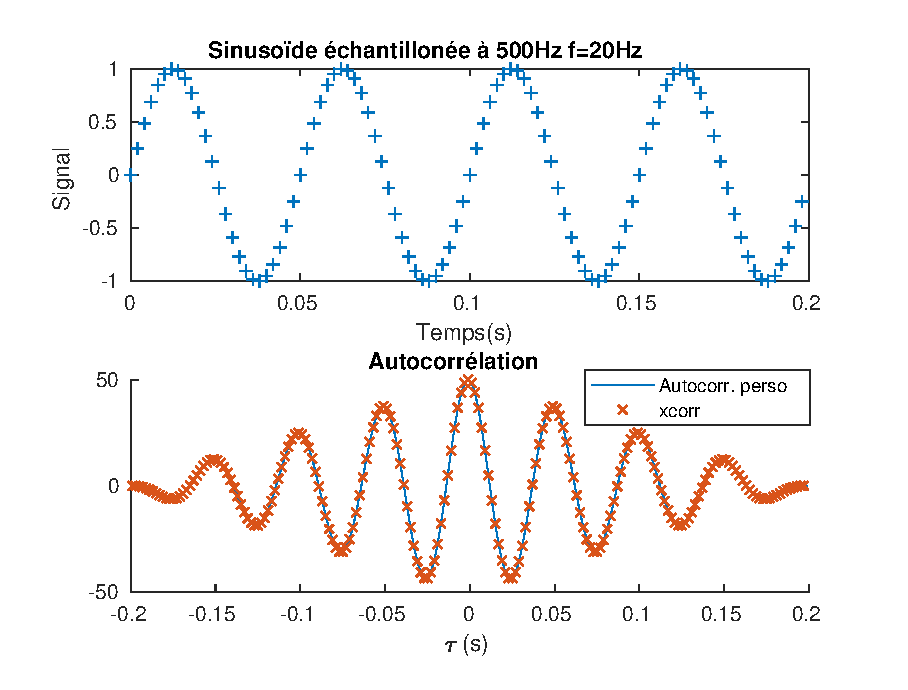
\includegraphics{images/autocorr.eps}
	\caption{Comparatif de de la fonction xcorr et de notre implémentation de l'autocorrélation.}
	\label{autocorr}
\end{figure}

La figure \ref{autocorr} montre que le résultat de \verb`xcorr` et de notre implémentation de l'autocorrélation sont identiques.

\paragraph{Remarque}
Nous n'avions d'abord tracé que la partie positive, avant de nous rendre compte de la nécessité de tracer également la partie négative.
On obtient un résultat différent du résultat théorique car le support de notre signal est fini, ce qui donne un cosinus amorti de manière symétrique et non un simple cosinus.

\section{ Application à la classification de quelques signaux simples}

Lorsque le signal se "répète" au cours du temps son autocorrélation est semblable sur de courtes périodes (reproduction du même motif au cours des périodes), on dit alors que le signal est stationnaire. Par contre si son autocorrélation est presque nulle, cela veut dire qu'il n'y a pas reproduction des motifs au cour des périodes et donc que le signal est non stationnaire.

\begin{figure}[h!]
	\centering
	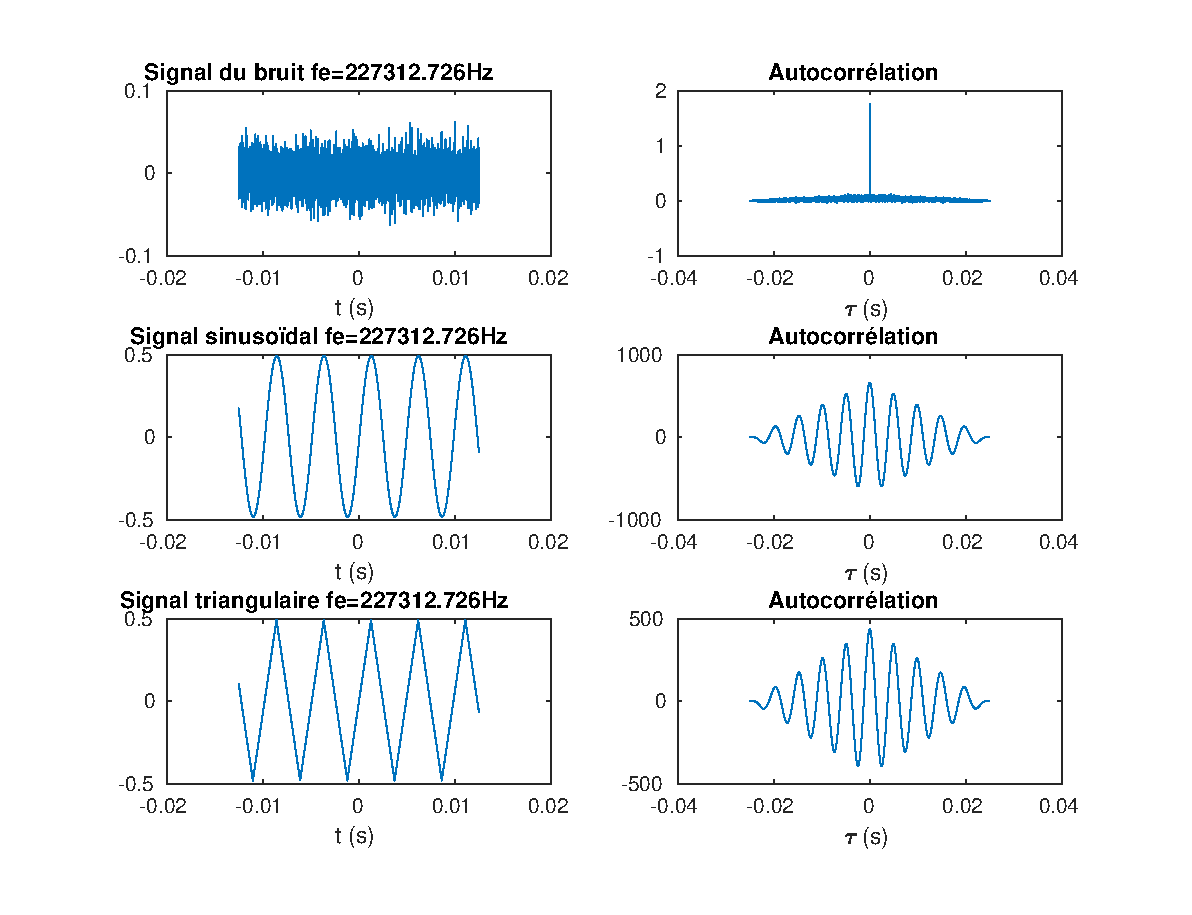
\includegraphics[width=1\textwidth]{images/classificationSig.eps}
	\caption{Autocorrélation de plusieurs signaux.}
	\label{classifSig}
\end{figure}

La figure \ref{classifSig} montre que les signaux sinusoïdaux et triangulaires sont stationnaires, contrairement au signal du bruit.

\begin{figure}[h!]
\centering
%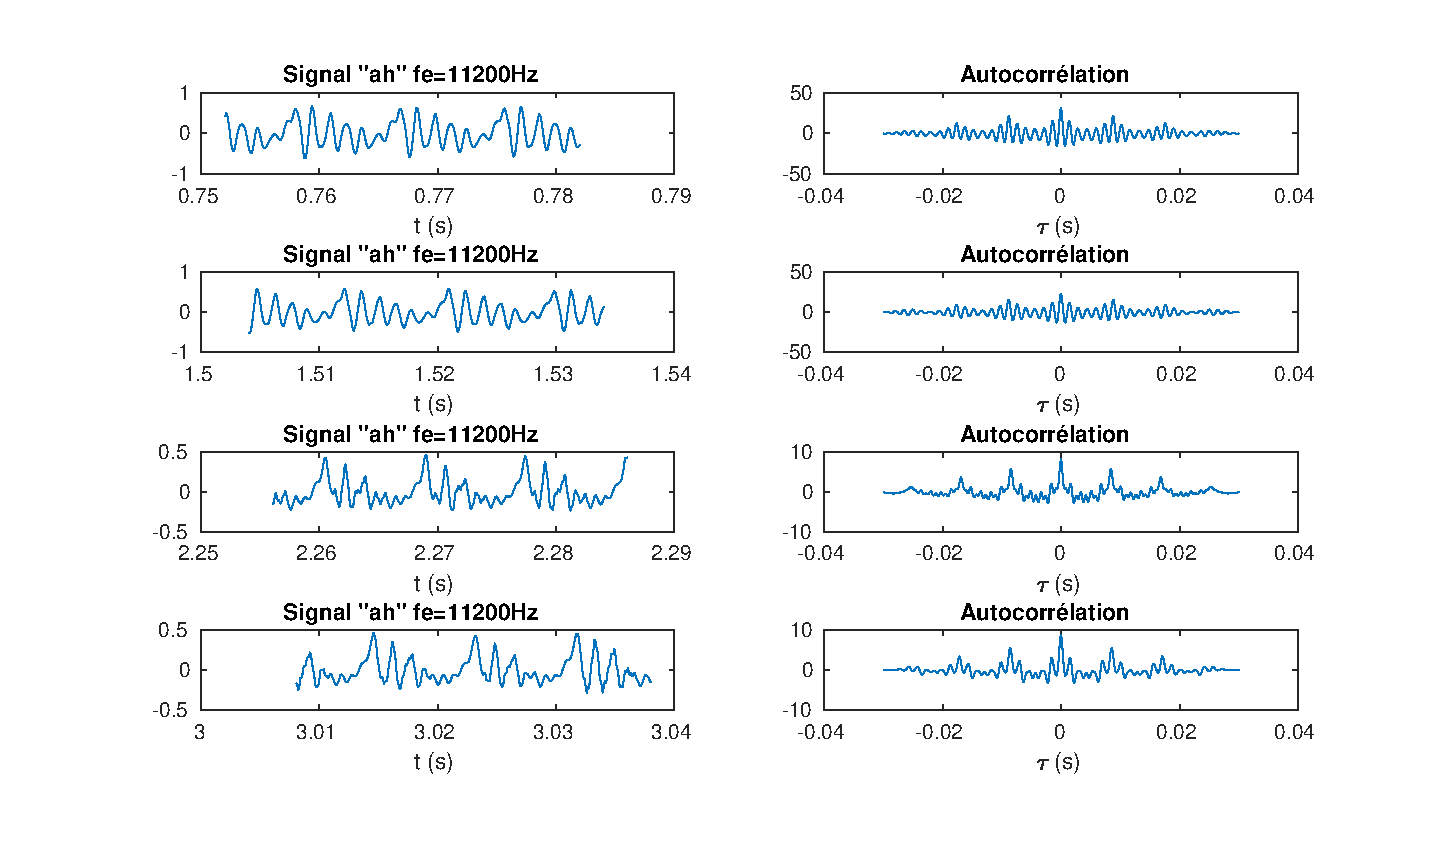
\includegraphics[width=\textwidth]{images/classificationAh.eps}
% Title: glps_renderer figure
% Creator: GL2PS 1.3.8, (C) 1999-2012 C. Geuzaine
% For: Octave
% CreationDate: Wed Nov  8 11:14:12 2017
\begin{pgfpicture}
\pgfsetlinewidth{0.01pt}
\color[rgb]{1.000000,1.000000,1.000000}
\pgfpathmoveto{\pgfpoint{335.117401pt}{386.837402pt}}
\pgflineto{\pgfpoint{521.279968pt}{340.136108pt}}
\pgflineto{\pgfpoint{335.117401pt}{340.136108pt}}
\pgfpathclose
\pgfusepath{fill,stroke}
\pgfpathmoveto{\pgfpoint{335.117401pt}{386.837402pt}}
\pgflineto{\pgfpoint{521.279968pt}{386.837402pt}}
\pgflineto{\pgfpoint{521.279968pt}{340.136108pt}}
\pgfpathclose
\pgfusepath{fill,stroke}
\pgfpathmoveto{\pgfpoint{74.879791pt}{386.837402pt}}
\pgflineto{\pgfpoint{261.042572pt}{340.136108pt}}
\pgflineto{\pgfpoint{74.879791pt}{340.136108pt}}
\pgfpathclose
\pgfusepath{fill,stroke}
\pgfpathmoveto{\pgfpoint{74.879791pt}{386.837402pt}}
\pgflineto{\pgfpoint{261.042572pt}{386.837402pt}}
\pgflineto{\pgfpoint{261.042572pt}{340.136108pt}}
\pgfpathclose
\pgfusepath{fill,stroke}
\pgfpathmoveto{\pgfpoint{335.117401pt}{289.298706pt}}
\pgflineto{\pgfpoint{521.279968pt}{242.597412pt}}
\pgflineto{\pgfpoint{335.117401pt}{242.597412pt}}
\pgfpathclose
\pgfusepath{fill,stroke}
\pgfpathmoveto{\pgfpoint{335.117401pt}{289.298706pt}}
\pgflineto{\pgfpoint{521.279968pt}{289.298706pt}}
\pgflineto{\pgfpoint{521.279968pt}{242.597412pt}}
\pgfpathclose
\pgfusepath{fill,stroke}
\pgfpathmoveto{\pgfpoint{74.879517pt}{289.298706pt}}
\pgflineto{\pgfpoint{261.042297pt}{242.597412pt}}
\pgflineto{\pgfpoint{74.879517pt}{242.597412pt}}
\pgfpathclose
\pgfusepath{fill,stroke}
\pgfpathmoveto{\pgfpoint{74.879517pt}{289.298706pt}}
\pgflineto{\pgfpoint{261.042297pt}{289.298706pt}}
\pgflineto{\pgfpoint{261.042297pt}{242.597412pt}}
\pgfpathclose
\pgfusepath{fill,stroke}
\pgfpathmoveto{\pgfpoint{335.117401pt}{191.760010pt}}
\pgflineto{\pgfpoint{521.279968pt}{145.058716pt}}
\pgflineto{\pgfpoint{335.117401pt}{145.058716pt}}
\pgfpathclose
\pgfusepath{fill,stroke}
\pgfpathmoveto{\pgfpoint{335.117401pt}{191.760010pt}}
\pgflineto{\pgfpoint{521.279968pt}{191.760010pt}}
\pgflineto{\pgfpoint{521.279968pt}{145.058716pt}}
\pgfpathclose
\pgfusepath{fill,stroke}
\pgfpathmoveto{\pgfpoint{74.879517pt}{191.760010pt}}
\pgflineto{\pgfpoint{261.041748pt}{145.058716pt}}
\pgflineto{\pgfpoint{74.879517pt}{145.058716pt}}
\pgfpathclose
\pgfusepath{fill,stroke}
\pgfpathmoveto{\pgfpoint{74.879517pt}{191.760010pt}}
\pgflineto{\pgfpoint{261.041748pt}{191.760010pt}}
\pgflineto{\pgfpoint{261.041748pt}{145.058716pt}}
\pgfpathclose
\pgfusepath{fill,stroke}
\pgfpathmoveto{\pgfpoint{335.117401pt}{94.221275pt}}
\pgflineto{\pgfpoint{521.279968pt}{47.519974pt}}
\pgflineto{\pgfpoint{335.117401pt}{47.519974pt}}
\pgfpathclose
\pgfusepath{fill,stroke}
\pgfpathmoveto{\pgfpoint{335.117401pt}{94.221275pt}}
\pgflineto{\pgfpoint{521.279968pt}{94.221275pt}}
\pgflineto{\pgfpoint{521.279968pt}{47.519974pt}}
\pgfpathclose
\pgfusepath{fill,stroke}
\pgfpathmoveto{\pgfpoint{74.881714pt}{94.221268pt}}
\pgflineto{\pgfpoint{261.043945pt}{47.519974pt}}
\pgflineto{\pgfpoint{74.881714pt}{47.519974pt}}
\pgfpathclose
\pgfusepath{fill,stroke}
\pgfpathmoveto{\pgfpoint{74.881714pt}{94.221268pt}}
\pgflineto{\pgfpoint{261.043945pt}{94.221268pt}}
\pgflineto{\pgfpoint{261.043945pt}{47.519974pt}}
\pgfpathclose
\pgfusepath{fill,stroke}
\color[rgb]{0.000000,0.000000,0.000000}
\pgfsetlinewidth{0.500000pt}
\pgfsetdash{{16pt}{0pt}}{0pt}
\pgfpathmoveto{\pgfpoint{521.279968pt}{340.136108pt}}
\pgflineto{\pgfpoint{335.117401pt}{340.136108pt}}
\pgfusepath{stroke}
\pgfpathmoveto{\pgfpoint{521.279968pt}{386.837402pt}}
\pgflineto{\pgfpoint{335.117401pt}{386.837402pt}}
\pgfusepath{stroke}
\pgfpathmoveto{\pgfpoint{335.117401pt}{386.837402pt}}
\pgflineto{\pgfpoint{335.117401pt}{340.136108pt}}
\pgfusepath{stroke}
\pgfpathmoveto{\pgfpoint{521.279968pt}{386.837402pt}}
\pgflineto{\pgfpoint{521.279968pt}{340.136108pt}}
\pgfusepath{stroke}
\pgfpathmoveto{\pgfpoint{335.117401pt}{341.985931pt}}
\pgflineto{\pgfpoint{335.117401pt}{340.136108pt}}
\pgfusepath{stroke}
\pgfpathmoveto{\pgfpoint{335.117401pt}{384.987610pt}}
\pgflineto{\pgfpoint{335.117401pt}{386.837402pt}}
\pgfusepath{stroke}
\pgfpathmoveto{\pgfpoint{381.658051pt}{341.985931pt}}
\pgflineto{\pgfpoint{381.658051pt}{340.136108pt}}
\pgfusepath{stroke}
\pgfpathmoveto{\pgfpoint{381.658051pt}{384.987610pt}}
\pgflineto{\pgfpoint{381.658051pt}{386.837402pt}}
\pgfusepath{stroke}
\pgfpathmoveto{\pgfpoint{428.198700pt}{341.985931pt}}
\pgflineto{\pgfpoint{428.198700pt}{340.136108pt}}
\pgfusepath{stroke}
\pgfpathmoveto{\pgfpoint{428.198700pt}{384.987610pt}}
\pgflineto{\pgfpoint{428.198700pt}{386.837402pt}}
\pgfusepath{stroke}
\pgfpathmoveto{\pgfpoint{474.739319pt}{341.985931pt}}
\pgflineto{\pgfpoint{474.739319pt}{340.136108pt}}
\pgfusepath{stroke}
\pgfpathmoveto{\pgfpoint{474.739319pt}{384.987610pt}}
\pgflineto{\pgfpoint{474.739319pt}{386.837402pt}}
\pgfusepath{stroke}
\pgfpathmoveto{\pgfpoint{521.279968pt}{341.985931pt}}
\pgflineto{\pgfpoint{521.279968pt}{340.136108pt}}
\pgfusepath{stroke}
\pgfpathmoveto{\pgfpoint{521.279968pt}{384.987610pt}}
\pgflineto{\pgfpoint{521.279968pt}{386.837402pt}}
\pgfusepath{stroke}
{
\pgftransformshift{\pgfpoint{335.117401pt}{335.167908pt}}
\pgfnode{rectangle}{north}{\fontsize{10}{0}\selectfont\textcolor[rgb]{0,0,0}{{-0.04}}}{}{\pgfusepath{discard}}}
{
\pgftransformshift{\pgfpoint{381.658051pt}{335.167908pt}}
\pgfnode{rectangle}{north}{\fontsize{10}{0}\selectfont\textcolor[rgb]{0,0,0}{{-0.02}}}{}{\pgfusepath{discard}}}
{
\pgftransformshift{\pgfpoint{428.198700pt}{335.167908pt}}
\pgfnode{rectangle}{north}{\fontsize{10}{0}\selectfont\textcolor[rgb]{0,0,0}{{0}}}{}{\pgfusepath{discard}}}
{
\pgftransformshift{\pgfpoint{474.739319pt}{335.167908pt}}
\pgfnode{rectangle}{north}{\fontsize{10}{0}\selectfont\textcolor[rgb]{0,0,0}{{0.02}}}{}{\pgfusepath{discard}}}
{
\pgftransformshift{\pgfpoint{521.279968pt}{335.167908pt}}
\pgfnode{rectangle}{north}{\fontsize{10}{0}\selectfont\textcolor[rgb]{0,0,0}{{0.04}}}{}{\pgfusepath{discard}}}
\pgfpathmoveto{\pgfpoint{336.980652pt}{340.136108pt}}
\pgflineto{\pgfpoint{335.117401pt}{340.136108pt}}
\pgfusepath{stroke}
\pgfpathmoveto{\pgfpoint{519.416748pt}{340.136108pt}}
\pgflineto{\pgfpoint{521.279968pt}{340.136108pt}}
\pgfusepath{stroke}
\pgfpathmoveto{\pgfpoint{336.980652pt}{347.919678pt}}
\pgflineto{\pgfpoint{335.117401pt}{347.919678pt}}
\pgfusepath{stroke}
\pgfpathmoveto{\pgfpoint{519.416748pt}{347.919678pt}}
\pgflineto{\pgfpoint{521.279968pt}{347.919678pt}}
\pgfusepath{stroke}
\pgfpathmoveto{\pgfpoint{336.980652pt}{355.703217pt}}
\pgflineto{\pgfpoint{335.117401pt}{355.703217pt}}
\pgfusepath{stroke}
\pgfpathmoveto{\pgfpoint{519.416748pt}{355.703217pt}}
\pgflineto{\pgfpoint{521.279968pt}{355.703217pt}}
\pgfusepath{stroke}
\pgfpathmoveto{\pgfpoint{336.980652pt}{363.486755pt}}
\pgflineto{\pgfpoint{335.117401pt}{363.486755pt}}
\pgfusepath{stroke}
\pgfpathmoveto{\pgfpoint{519.416748pt}{363.486755pt}}
\pgflineto{\pgfpoint{521.279968pt}{363.486755pt}}
\pgfusepath{stroke}
\pgfpathmoveto{\pgfpoint{336.980652pt}{371.270325pt}}
\pgflineto{\pgfpoint{335.117401pt}{371.270325pt}}
\pgfusepath{stroke}
\pgfpathmoveto{\pgfpoint{519.416748pt}{371.270325pt}}
\pgflineto{\pgfpoint{521.279968pt}{371.270325pt}}
\pgfusepath{stroke}
\pgfpathmoveto{\pgfpoint{336.980652pt}{379.053864pt}}
\pgflineto{\pgfpoint{335.117401pt}{379.053864pt}}
\pgfusepath{stroke}
\pgfpathmoveto{\pgfpoint{519.416748pt}{379.053864pt}}
\pgflineto{\pgfpoint{521.279968pt}{379.053864pt}}
\pgfusepath{stroke}
\pgfpathmoveto{\pgfpoint{336.980652pt}{386.837402pt}}
\pgflineto{\pgfpoint{335.117401pt}{386.837402pt}}
\pgfusepath{stroke}
\pgfpathmoveto{\pgfpoint{519.416748pt}{386.837402pt}}
\pgflineto{\pgfpoint{521.279968pt}{386.837402pt}}
\pgfusepath{stroke}
{
\pgftransformshift{\pgfpoint{330.113037pt}{340.136108pt}}
\pgfnode{rectangle}{east}{\fontsize{10}{0}\selectfont\textcolor[rgb]{0,0,0}{{-20}}}{}{\pgfusepath{discard}}}
{
\pgftransformshift{\pgfpoint{330.113037pt}{347.919678pt}}
\pgfnode{rectangle}{east}{\fontsize{10}{0}\selectfont\textcolor[rgb]{0,0,0}{{-10}}}{}{\pgfusepath{discard}}}
{
\pgftransformshift{\pgfpoint{330.113037pt}{355.703217pt}}
\pgfnode{rectangle}{east}{\fontsize{10}{0}\selectfont\textcolor[rgb]{0,0,0}{{0}}}{}{\pgfusepath{discard}}}
{
\pgftransformshift{\pgfpoint{330.113037pt}{363.486755pt}}
\pgfnode{rectangle}{east}{\fontsize{10}{0}\selectfont\textcolor[rgb]{0,0,0}{{10}}}{}{\pgfusepath{discard}}}
{
\pgftransformshift{\pgfpoint{330.113037pt}{371.270325pt}}
\pgfnode{rectangle}{east}{\fontsize{10}{0}\selectfont\textcolor[rgb]{0,0,0}{{20}}}{}{\pgfusepath{discard}}}
{
\pgftransformshift{\pgfpoint{330.113037pt}{379.053864pt}}
\pgfnode{rectangle}{east}{\fontsize{10}{0}\selectfont\textcolor[rgb]{0,0,0}{{30}}}{}{\pgfusepath{discard}}}
{
\pgftransformshift{\pgfpoint{330.113037pt}{386.837402pt}}
\pgfnode{rectangle}{east}{\fontsize{10}{0}\selectfont\textcolor[rgb]{0,0,0}{{40}}}{}{\pgfusepath{discard}}}
{
\pgftransformshift{\pgfpoint{428.198700pt}{324.167908pt}}
\pgfnode{rectangle}{north}{\fontsize{10}{0}\selectfont\textcolor[rgb]{0,0,0}{{$\tau$ (s)}}}{}{\pgfusepath{discard}}}
\color[rgb]{0.000000,0.000000,1.000000}
\pgfsetdash{}{0pt}
\pgfpathmoveto{\pgfpoint{358.491608pt}{355.494690pt}}
\pgflineto{\pgfpoint{358.283844pt}{355.614929pt}}
\pgfusepath{stroke}
\pgfpathmoveto{\pgfpoint{358.699371pt}{355.378540pt}}
\pgflineto{\pgfpoint{358.491608pt}{355.494690pt}}
\pgfusepath{stroke}
\pgfpathmoveto{\pgfpoint{358.907166pt}{355.295349pt}}
\pgflineto{\pgfpoint{358.699371pt}{355.378540pt}}
\pgfusepath{stroke}
\pgfpathmoveto{\pgfpoint{359.114929pt}{355.269836pt}}
\pgflineto{\pgfpoint{358.907166pt}{355.295349pt}}
\pgfusepath{stroke}
\pgfpathmoveto{\pgfpoint{359.322693pt}{355.333252pt}}
\pgflineto{\pgfpoint{359.114929pt}{355.269836pt}}
\pgfusepath{stroke}
\pgfpathmoveto{\pgfpoint{359.530457pt}{355.485718pt}}
\pgflineto{\pgfpoint{359.322693pt}{355.333252pt}}
\pgfusepath{stroke}
\pgfpathmoveto{\pgfpoint{359.738220pt}{355.704468pt}}
\pgflineto{\pgfpoint{359.530457pt}{355.485718pt}}
\pgfusepath{stroke}
\pgfpathmoveto{\pgfpoint{359.946014pt}{355.953278pt}}
\pgflineto{\pgfpoint{359.738220pt}{355.704468pt}}
\pgfusepath{stroke}
\pgfpathmoveto{\pgfpoint{360.153778pt}{356.169586pt}}
\pgflineto{\pgfpoint{359.946014pt}{355.953278pt}}
\pgfusepath{stroke}
\pgfpathmoveto{\pgfpoint{360.361572pt}{356.290039pt}}
\pgflineto{\pgfpoint{360.153778pt}{356.169586pt}}
\pgfusepath{stroke}
\pgfpathmoveto{\pgfpoint{360.569305pt}{356.275330pt}}
\pgflineto{\pgfpoint{360.361572pt}{356.290039pt}}
\pgfusepath{stroke}
\pgfpathmoveto{\pgfpoint{360.777100pt}{356.106781pt}}
\pgflineto{\pgfpoint{360.569305pt}{356.275330pt}}
\pgfusepath{stroke}
\pgfpathmoveto{\pgfpoint{360.984863pt}{355.811493pt}}
\pgflineto{\pgfpoint{360.777100pt}{356.106781pt}}
\pgfusepath{stroke}
\pgfpathmoveto{\pgfpoint{361.192627pt}{355.451172pt}}
\pgflineto{\pgfpoint{360.984863pt}{355.811493pt}}
\pgfusepath{stroke}
\pgfpathmoveto{\pgfpoint{361.400391pt}{355.110657pt}}
\pgflineto{\pgfpoint{361.192627pt}{355.451172pt}}
\pgfusepath{stroke}
\pgfpathmoveto{\pgfpoint{361.608185pt}{354.868469pt}}
\pgflineto{\pgfpoint{361.400391pt}{355.110657pt}}
\pgfusepath{stroke}
\pgfpathmoveto{\pgfpoint{361.815948pt}{354.777588pt}}
\pgflineto{\pgfpoint{361.608185pt}{354.868469pt}}
\pgfusepath{stroke}
\pgfpathmoveto{\pgfpoint{362.023712pt}{354.867615pt}}
\pgflineto{\pgfpoint{361.815948pt}{354.777588pt}}
\pgfusepath{stroke}
\pgfpathmoveto{\pgfpoint{362.231476pt}{355.127411pt}}
\pgflineto{\pgfpoint{362.023712pt}{354.867615pt}}
\pgfusepath{stroke}
\pgfpathmoveto{\pgfpoint{362.439270pt}{355.516052pt}}
\pgflineto{\pgfpoint{362.231476pt}{355.127411pt}}
\pgfusepath{stroke}
\pgfpathmoveto{\pgfpoint{362.647034pt}{355.963440pt}}
\pgflineto{\pgfpoint{362.439270pt}{355.516052pt}}
\pgfusepath{stroke}
\pgfpathmoveto{\pgfpoint{362.854797pt}{356.386475pt}}
\pgflineto{\pgfpoint{362.647034pt}{355.963440pt}}
\pgfusepath{stroke}
\pgfpathmoveto{\pgfpoint{363.062561pt}{356.720459pt}}
\pgflineto{\pgfpoint{362.854797pt}{356.386475pt}}
\pgfusepath{stroke}
\pgfpathmoveto{\pgfpoint{363.270325pt}{356.923401pt}}
\pgflineto{\pgfpoint{363.062561pt}{356.720459pt}}
\pgfusepath{stroke}
\pgfpathmoveto{\pgfpoint{363.478119pt}{356.974182pt}}
\pgflineto{\pgfpoint{363.270325pt}{356.923401pt}}
\pgfusepath{stroke}
\pgfpathmoveto{\pgfpoint{363.685883pt}{356.863190pt}}
\pgflineto{\pgfpoint{363.478119pt}{356.974182pt}}
\pgfusepath{stroke}
\pgfpathmoveto{\pgfpoint{363.893677pt}{356.597534pt}}
\pgflineto{\pgfpoint{363.685883pt}{356.863190pt}}
\pgfusepath{stroke}
\pgfpathmoveto{\pgfpoint{364.101410pt}{356.200928pt}}
\pgflineto{\pgfpoint{363.893677pt}{356.597534pt}}
\pgfusepath{stroke}
\pgfpathmoveto{\pgfpoint{364.309204pt}{355.719452pt}}
\pgflineto{\pgfpoint{364.101410pt}{356.200928pt}}
\pgfusepath{stroke}
\pgfpathmoveto{\pgfpoint{364.516968pt}{355.221466pt}}
\pgflineto{\pgfpoint{364.309204pt}{355.719452pt}}
\pgfusepath{stroke}
\pgfpathmoveto{\pgfpoint{364.724731pt}{354.788239pt}}
\pgflineto{\pgfpoint{364.516968pt}{355.221466pt}}
\pgfusepath{stroke}
\pgfpathmoveto{\pgfpoint{364.932495pt}{354.517334pt}}
\pgflineto{\pgfpoint{364.724731pt}{354.788239pt}}
\pgfusepath{stroke}
\pgfpathmoveto{\pgfpoint{365.140289pt}{354.496033pt}}
\pgflineto{\pgfpoint{364.932495pt}{354.517334pt}}
\pgfusepath{stroke}
\pgfpathmoveto{\pgfpoint{365.348022pt}{354.762512pt}}
\pgflineto{\pgfpoint{365.140289pt}{354.496033pt}}
\pgfusepath{stroke}
\pgfpathmoveto{\pgfpoint{365.555817pt}{355.303162pt}}
\pgflineto{\pgfpoint{365.348022pt}{354.762512pt}}
\pgfusepath{stroke}
\pgfpathmoveto{\pgfpoint{365.763580pt}{356.044678pt}}
\pgflineto{\pgfpoint{365.555817pt}{355.303162pt}}
\pgfusepath{stroke}
\pgfpathmoveto{\pgfpoint{365.971375pt}{356.851562pt}}
\pgflineto{\pgfpoint{365.763580pt}{356.044678pt}}
\pgfusepath{stroke}
\pgfpathmoveto{\pgfpoint{366.179138pt}{357.570953pt}}
\pgflineto{\pgfpoint{365.971375pt}{356.851562pt}}
\pgfusepath{stroke}
\pgfpathmoveto{\pgfpoint{366.386902pt}{358.049988pt}}
\pgflineto{\pgfpoint{366.179138pt}{357.570953pt}}
\pgfusepath{stroke}
\pgfpathmoveto{\pgfpoint{366.594666pt}{358.167664pt}}
\pgflineto{\pgfpoint{366.386902pt}{358.049988pt}}
\pgfusepath{stroke}
\pgfpathmoveto{\pgfpoint{366.802429pt}{357.898102pt}}
\pgflineto{\pgfpoint{366.594666pt}{358.167664pt}}
\pgfusepath{stroke}
\pgfpathmoveto{\pgfpoint{367.010223pt}{357.309021pt}}
\pgflineto{\pgfpoint{366.802429pt}{357.898102pt}}
\pgfusepath{stroke}
\pgfpathmoveto{\pgfpoint{367.217987pt}{356.515137pt}}
\pgflineto{\pgfpoint{367.010223pt}{357.309021pt}}
\pgfusepath{stroke}
\pgfpathmoveto{\pgfpoint{367.425751pt}{355.672485pt}}
\pgflineto{\pgfpoint{367.217987pt}{356.515137pt}}
\pgfusepath{stroke}
\pgfpathmoveto{\pgfpoint{367.633514pt}{354.936707pt}}
\pgflineto{\pgfpoint{367.425751pt}{355.672485pt}}
\pgfusepath{stroke}
\pgfpathmoveto{\pgfpoint{367.841309pt}{354.417664pt}}
\pgflineto{\pgfpoint{367.633514pt}{354.936707pt}}
\pgfusepath{stroke}
\pgfpathmoveto{\pgfpoint{368.049072pt}{354.190033pt}}
\pgflineto{\pgfpoint{367.841309pt}{354.417664pt}}
\pgfusepath{stroke}
\pgfpathmoveto{\pgfpoint{368.256836pt}{354.269653pt}}
\pgflineto{\pgfpoint{368.049072pt}{354.190033pt}}
\pgfusepath{stroke}
\pgfpathmoveto{\pgfpoint{368.464600pt}{354.608154pt}}
\pgflineto{\pgfpoint{368.256836pt}{354.269653pt}}
\pgfusepath{stroke}
\pgfpathmoveto{\pgfpoint{368.672363pt}{355.136078pt}}
\pgflineto{\pgfpoint{368.464600pt}{354.608154pt}}
\pgfusepath{stroke}
\pgfpathmoveto{\pgfpoint{368.880127pt}{355.794647pt}}
\pgflineto{\pgfpoint{368.672363pt}{355.136078pt}}
\pgfusepath{stroke}
\pgfpathmoveto{\pgfpoint{369.087921pt}{356.510071pt}}
\pgflineto{\pgfpoint{368.880127pt}{355.794647pt}}
\pgfusepath{stroke}
\pgfpathmoveto{\pgfpoint{369.295685pt}{357.198730pt}}
\pgflineto{\pgfpoint{369.087921pt}{356.510071pt}}
\pgfusepath{stroke}
\pgfpathmoveto{\pgfpoint{369.503479pt}{357.778992pt}}
\pgflineto{\pgfpoint{369.295685pt}{357.198730pt}}
\pgfusepath{stroke}
\pgfpathmoveto{\pgfpoint{369.711243pt}{358.151947pt}}
\pgflineto{\pgfpoint{369.503479pt}{357.778992pt}}
\pgfusepath{stroke}
\pgfpathmoveto{\pgfpoint{369.919006pt}{358.217407pt}}
\pgflineto{\pgfpoint{369.711243pt}{358.151947pt}}
\pgfusepath{stroke}
\pgfpathmoveto{\pgfpoint{370.126770pt}{357.923828pt}}
\pgflineto{\pgfpoint{369.919006pt}{358.217407pt}}
\pgfusepath{stroke}
\pgfpathmoveto{\pgfpoint{370.334534pt}{357.249939pt}}
\pgflineto{\pgfpoint{370.126770pt}{357.923828pt}}
\pgfusepath{stroke}
\pgfpathmoveto{\pgfpoint{370.542297pt}{356.256042pt}}
\pgflineto{\pgfpoint{370.334534pt}{357.249939pt}}
\pgfusepath{stroke}
\pgfpathmoveto{\pgfpoint{370.750092pt}{355.107513pt}}
\pgflineto{\pgfpoint{370.542297pt}{356.256042pt}}
\pgfusepath{stroke}
\pgfpathmoveto{\pgfpoint{370.957855pt}{354.006927pt}}
\pgflineto{\pgfpoint{370.750092pt}{355.107513pt}}
\pgfusepath{stroke}
\pgfpathmoveto{\pgfpoint{371.165619pt}{353.154602pt}}
\pgflineto{\pgfpoint{370.957855pt}{354.006927pt}}
\pgfusepath{stroke}
\pgfpathmoveto{\pgfpoint{371.373413pt}{352.710358pt}}
\pgflineto{\pgfpoint{371.165619pt}{353.154602pt}}
\pgfusepath{stroke}
\pgfpathmoveto{\pgfpoint{371.581177pt}{352.751709pt}}
\pgflineto{\pgfpoint{371.373413pt}{352.710358pt}}
\pgfusepath{stroke}
\pgfpathmoveto{\pgfpoint{371.788940pt}{353.257690pt}}
\pgflineto{\pgfpoint{371.581177pt}{352.751709pt}}
\pgfusepath{stroke}
\pgfpathmoveto{\pgfpoint{371.996704pt}{354.125793pt}}
\pgflineto{\pgfpoint{371.788940pt}{353.257690pt}}
\pgfusepath{stroke}
\pgfpathmoveto{\pgfpoint{372.204498pt}{355.174042pt}}
\pgflineto{\pgfpoint{371.996704pt}{354.125793pt}}
\pgfusepath{stroke}
\pgfpathmoveto{\pgfpoint{372.412231pt}{356.179321pt}}
\pgflineto{\pgfpoint{372.204498pt}{355.174042pt}}
\pgfusepath{stroke}
\pgfpathmoveto{\pgfpoint{372.620026pt}{356.966766pt}}
\pgflineto{\pgfpoint{372.412231pt}{356.179321pt}}
\pgfusepath{stroke}
\pgfpathmoveto{\pgfpoint{372.827789pt}{357.444916pt}}
\pgflineto{\pgfpoint{372.620026pt}{356.966766pt}}
\pgfusepath{stroke}
\pgfpathmoveto{\pgfpoint{373.035553pt}{357.590820pt}}
\pgflineto{\pgfpoint{372.827789pt}{357.444916pt}}
\pgfusepath{stroke}
\pgfpathmoveto{\pgfpoint{373.243347pt}{357.437836pt}}
\pgflineto{\pgfpoint{373.035553pt}{357.590820pt}}
\pgfusepath{stroke}
\pgfpathmoveto{\pgfpoint{373.451111pt}{357.053741pt}}
\pgflineto{\pgfpoint{373.243347pt}{357.437836pt}}
\pgfusepath{stroke}
\pgfpathmoveto{\pgfpoint{373.658875pt}{356.500122pt}}
\pgflineto{\pgfpoint{373.451111pt}{357.053741pt}}
\pgfusepath{stroke}
\pgfpathmoveto{\pgfpoint{373.866638pt}{355.836914pt}}
\pgflineto{\pgfpoint{373.658875pt}{356.500122pt}}
\pgfusepath{stroke}
\pgfpathmoveto{\pgfpoint{374.074402pt}{355.150696pt}}
\pgflineto{\pgfpoint{373.866638pt}{355.836914pt}}
\pgfusepath{stroke}
\pgfpathmoveto{\pgfpoint{374.282196pt}{354.512207pt}}
\pgflineto{\pgfpoint{374.074402pt}{355.150696pt}}
\pgfusepath{stroke}
\pgfpathmoveto{\pgfpoint{374.489960pt}{353.978882pt}}
\pgflineto{\pgfpoint{374.282196pt}{354.512207pt}}
\pgfusepath{stroke}
\pgfpathmoveto{\pgfpoint{374.697723pt}{353.615417pt}}
\pgflineto{\pgfpoint{374.489960pt}{353.978882pt}}
\pgfusepath{stroke}
\pgfpathmoveto{\pgfpoint{374.905487pt}{353.453857pt}}
\pgflineto{\pgfpoint{374.697723pt}{353.615417pt}}
\pgfusepath{stroke}
\pgfpathmoveto{\pgfpoint{375.113281pt}{353.510315pt}}
\pgflineto{\pgfpoint{374.905487pt}{353.453857pt}}
\pgfusepath{stroke}
\pgfpathmoveto{\pgfpoint{375.321045pt}{353.791107pt}}
\pgflineto{\pgfpoint{375.113281pt}{353.510315pt}}
\pgfusepath{stroke}
\pgfpathmoveto{\pgfpoint{375.528809pt}{354.268921pt}}
\pgflineto{\pgfpoint{375.321045pt}{353.791107pt}}
\pgfusepath{stroke}
\pgfpathmoveto{\pgfpoint{375.736572pt}{354.874573pt}}
\pgflineto{\pgfpoint{375.528809pt}{354.268921pt}}
\pgfusepath{stroke}
\pgfpathmoveto{\pgfpoint{375.944336pt}{355.535675pt}}
\pgflineto{\pgfpoint{375.736572pt}{354.874573pt}}
\pgfusepath{stroke}
\pgfpathmoveto{\pgfpoint{376.152130pt}{356.169067pt}}
\pgflineto{\pgfpoint{375.944336pt}{355.535675pt}}
\pgfusepath{stroke}
\pgfpathmoveto{\pgfpoint{376.359894pt}{356.685974pt}}
\pgflineto{\pgfpoint{376.152130pt}{356.169067pt}}
\pgfusepath{stroke}
\pgfpathmoveto{\pgfpoint{376.567688pt}{357.030731pt}}
\pgflineto{\pgfpoint{376.359894pt}{356.685974pt}}
\pgfusepath{stroke}
\pgfpathmoveto{\pgfpoint{376.775452pt}{357.163025pt}}
\pgflineto{\pgfpoint{376.567688pt}{357.030731pt}}
\pgfusepath{stroke}
\pgfpathmoveto{\pgfpoint{376.983215pt}{357.062927pt}}
\pgflineto{\pgfpoint{376.775452pt}{357.163025pt}}
\pgfusepath{stroke}
\pgfpathmoveto{\pgfpoint{377.190979pt}{356.747742pt}}
\pgflineto{\pgfpoint{376.983215pt}{357.062927pt}}
\pgfusepath{stroke}
\pgfpathmoveto{\pgfpoint{377.398743pt}{356.258057pt}}
\pgflineto{\pgfpoint{377.190979pt}{356.747742pt}}
\pgfusepath{stroke}
\pgfpathmoveto{\pgfpoint{377.606506pt}{355.639221pt}}
\pgflineto{\pgfpoint{377.398743pt}{356.258057pt}}
\pgfusepath{stroke}
\pgfpathmoveto{\pgfpoint{377.814301pt}{354.968811pt}}
\pgflineto{\pgfpoint{377.606506pt}{355.639221pt}}
\pgfusepath{stroke}
\pgfpathmoveto{\pgfpoint{378.022064pt}{354.331970pt}}
\pgflineto{\pgfpoint{377.814301pt}{354.968811pt}}
\pgfusepath{stroke}
\pgfpathmoveto{\pgfpoint{378.229828pt}{353.803589pt}}
\pgflineto{\pgfpoint{378.022064pt}{354.331970pt}}
\pgfusepath{stroke}
\pgfpathmoveto{\pgfpoint{378.437592pt}{353.445618pt}}
\pgflineto{\pgfpoint{378.229828pt}{353.803589pt}}
\pgfusepath{stroke}
\pgfpathmoveto{\pgfpoint{378.645386pt}{353.299622pt}}
\pgflineto{\pgfpoint{378.437592pt}{353.445618pt}}
\pgfusepath{stroke}
\pgfpathmoveto{\pgfpoint{378.853149pt}{353.373047pt}}
\pgflineto{\pgfpoint{378.645386pt}{353.299622pt}}
\pgfusepath{stroke}
\pgfpathmoveto{\pgfpoint{379.060913pt}{353.659485pt}}
\pgflineto{\pgfpoint{378.853149pt}{353.373047pt}}
\pgfusepath{stroke}
\pgfpathmoveto{\pgfpoint{379.268677pt}{354.142273pt}}
\pgflineto{\pgfpoint{379.060913pt}{353.659485pt}}
\pgfusepath{stroke}
\pgfpathmoveto{\pgfpoint{379.476440pt}{354.774109pt}}
\pgflineto{\pgfpoint{379.268677pt}{354.142273pt}}
\pgfusepath{stroke}
\pgfpathmoveto{\pgfpoint{379.684204pt}{355.493408pt}}
\pgflineto{\pgfpoint{379.476440pt}{354.774109pt}}
\pgfusepath{stroke}
\pgfpathmoveto{\pgfpoint{379.891998pt}{356.235382pt}}
\pgflineto{\pgfpoint{379.684204pt}{355.493408pt}}
\pgfusepath{stroke}
\pgfpathmoveto{\pgfpoint{380.099762pt}{356.907379pt}}
\pgflineto{\pgfpoint{379.891998pt}{356.235382pt}}
\pgfusepath{stroke}
\pgfpathmoveto{\pgfpoint{380.307556pt}{357.408447pt}}
\pgflineto{\pgfpoint{380.099762pt}{356.907379pt}}
\pgfusepath{stroke}
\pgfpathmoveto{\pgfpoint{380.515320pt}{357.638885pt}}
\pgflineto{\pgfpoint{380.307556pt}{357.408447pt}}
\pgfusepath{stroke}
\pgfpathmoveto{\pgfpoint{380.723083pt}{357.505432pt}}
\pgflineto{\pgfpoint{380.515320pt}{357.638885pt}}
\pgfusepath{stroke}
\pgfpathmoveto{\pgfpoint{380.930847pt}{356.962280pt}}
\pgflineto{\pgfpoint{380.723083pt}{357.505432pt}}
\pgfusepath{stroke}
\pgfpathmoveto{\pgfpoint{381.138611pt}{356.036591pt}}
\pgflineto{\pgfpoint{380.930847pt}{356.962280pt}}
\pgfusepath{stroke}
\pgfpathmoveto{\pgfpoint{381.346375pt}{354.828308pt}}
\pgflineto{\pgfpoint{381.138611pt}{356.036591pt}}
\pgfusepath{stroke}
\pgfpathmoveto{\pgfpoint{381.554169pt}{353.530762pt}}
\pgflineto{\pgfpoint{381.346375pt}{354.828308pt}}
\pgfusepath{stroke}
\pgfpathmoveto{\pgfpoint{381.761932pt}{352.386810pt}}
\pgflineto{\pgfpoint{381.554169pt}{353.530762pt}}
\pgfusepath{stroke}
\pgfpathmoveto{\pgfpoint{381.969696pt}{351.631592pt}}
\pgflineto{\pgfpoint{381.761932pt}{352.386810pt}}
\pgfusepath{stroke}
\pgfpathmoveto{\pgfpoint{382.177490pt}{351.445526pt}}
\pgflineto{\pgfpoint{381.969696pt}{351.631592pt}}
\pgfusepath{stroke}
\pgfpathmoveto{\pgfpoint{382.385254pt}{351.905884pt}}
\pgflineto{\pgfpoint{382.177490pt}{351.445526pt}}
\pgfusepath{stroke}
\pgfpathmoveto{\pgfpoint{382.593018pt}{352.974182pt}}
\pgflineto{\pgfpoint{382.385254pt}{351.905884pt}}
\pgfusepath{stroke}
\pgfpathmoveto{\pgfpoint{382.800781pt}{354.504761pt}}
\pgflineto{\pgfpoint{382.593018pt}{352.974182pt}}
\pgfusepath{stroke}
\pgfpathmoveto{\pgfpoint{383.008545pt}{356.264587pt}}
\pgflineto{\pgfpoint{382.800781pt}{354.504761pt}}
\pgfusepath{stroke}
\pgfpathmoveto{\pgfpoint{383.216339pt}{357.971558pt}}
\pgflineto{\pgfpoint{383.008545pt}{356.264587pt}}
\pgfusepath{stroke}
\pgfpathmoveto{\pgfpoint{383.424103pt}{359.359955pt}}
\pgflineto{\pgfpoint{383.216339pt}{357.971558pt}}
\pgfusepath{stroke}
\pgfpathmoveto{\pgfpoint{383.631866pt}{360.231262pt}}
\pgflineto{\pgfpoint{383.424103pt}{359.359955pt}}
\pgfusepath{stroke}
\pgfpathmoveto{\pgfpoint{383.839661pt}{360.471619pt}}
\pgflineto{\pgfpoint{383.631866pt}{360.231262pt}}
\pgfusepath{stroke}
\pgfpathmoveto{\pgfpoint{384.047424pt}{360.048401pt}}
\pgflineto{\pgfpoint{383.839661pt}{360.471619pt}}
\pgfusepath{stroke}
\pgfpathmoveto{\pgfpoint{384.255188pt}{359.012024pt}}
\pgflineto{\pgfpoint{384.047424pt}{360.048401pt}}
\pgfusepath{stroke}
\pgfpathmoveto{\pgfpoint{384.462952pt}{357.485229pt}}
\pgflineto{\pgfpoint{384.255188pt}{359.012024pt}}
\pgfusepath{stroke}
\pgfpathmoveto{\pgfpoint{384.670715pt}{355.653076pt}}
\pgflineto{\pgfpoint{384.462952pt}{357.485229pt}}
\pgfusepath{stroke}
\pgfpathmoveto{\pgfpoint{384.878479pt}{353.772064pt}}
\pgflineto{\pgfpoint{384.670715pt}{355.653076pt}}
\pgfusepath{stroke}
\pgfpathmoveto{\pgfpoint{385.086273pt}{352.136078pt}}
\pgflineto{\pgfpoint{384.878479pt}{353.772064pt}}
\pgfusepath{stroke}
\pgfpathmoveto{\pgfpoint{385.294037pt}{351.051941pt}}
\pgflineto{\pgfpoint{385.086273pt}{352.136078pt}}
\pgfusepath{stroke}
\pgfpathmoveto{\pgfpoint{385.501801pt}{350.806274pt}}
\pgflineto{\pgfpoint{385.294037pt}{351.051941pt}}
\pgfusepath{stroke}
\pgfpathmoveto{\pgfpoint{385.709595pt}{351.570923pt}}
\pgflineto{\pgfpoint{385.501801pt}{350.806274pt}}
\pgfusepath{stroke}
\pgfpathmoveto{\pgfpoint{385.917358pt}{353.332642pt}}
\pgflineto{\pgfpoint{385.709595pt}{351.570923pt}}
\pgfusepath{stroke}
\pgfpathmoveto{\pgfpoint{386.125122pt}{355.896851pt}}
\pgflineto{\pgfpoint{385.917358pt}{353.332642pt}}
\pgfusepath{stroke}
\pgfpathmoveto{\pgfpoint{386.332886pt}{358.888977pt}}
\pgflineto{\pgfpoint{386.125122pt}{355.896851pt}}
\pgfusepath{stroke}
\pgfpathmoveto{\pgfpoint{386.540649pt}{361.792603pt}}
\pgflineto{\pgfpoint{386.332886pt}{358.888977pt}}
\pgfusepath{stroke}
\pgfpathmoveto{\pgfpoint{386.748413pt}{364.073059pt}}
\pgflineto{\pgfpoint{386.540649pt}{361.792603pt}}
\pgfusepath{stroke}
\pgfpathmoveto{\pgfpoint{386.956207pt}{365.272369pt}}
\pgflineto{\pgfpoint{386.748413pt}{364.073059pt}}
\pgfusepath{stroke}
\pgfpathmoveto{\pgfpoint{387.163971pt}{365.125275pt}}
\pgflineto{\pgfpoint{386.956207pt}{365.272369pt}}
\pgfusepath{stroke}
\pgfpathmoveto{\pgfpoint{387.371765pt}{363.677979pt}}
\pgflineto{\pgfpoint{387.163971pt}{365.125275pt}}
\pgfusepath{stroke}
\pgfpathmoveto{\pgfpoint{387.579529pt}{361.240845pt}}
\pgflineto{\pgfpoint{387.371765pt}{363.677979pt}}
\pgfusepath{stroke}
\pgfpathmoveto{\pgfpoint{387.787292pt}{358.273499pt}}
\pgflineto{\pgfpoint{387.579529pt}{361.240845pt}}
\pgfusepath{stroke}
\pgfpathmoveto{\pgfpoint{387.995056pt}{355.307373pt}}
\pgflineto{\pgfpoint{387.787292pt}{358.273499pt}}
\pgfusepath{stroke}
\pgfpathmoveto{\pgfpoint{388.202820pt}{352.826355pt}}
\pgflineto{\pgfpoint{387.995056pt}{355.307373pt}}
\pgfusepath{stroke}
\pgfpathmoveto{\pgfpoint{388.410583pt}{351.168793pt}}
\pgflineto{\pgfpoint{388.202820pt}{352.826355pt}}
\pgfusepath{stroke}
\pgfpathmoveto{\pgfpoint{388.618378pt}{350.517029pt}}
\pgflineto{\pgfpoint{388.410583pt}{351.168793pt}}
\pgfusepath{stroke}
\pgfpathmoveto{\pgfpoint{388.826141pt}{350.867188pt}}
\pgflineto{\pgfpoint{388.618378pt}{350.517029pt}}
\pgfusepath{stroke}
\pgfpathmoveto{\pgfpoint{389.033905pt}{352.044861pt}}
\pgflineto{\pgfpoint{388.826141pt}{350.867188pt}}
\pgfusepath{stroke}
\pgfpathmoveto{\pgfpoint{389.241699pt}{353.806915pt}}
\pgflineto{\pgfpoint{389.033905pt}{352.044861pt}}
\pgfusepath{stroke}
\pgfpathmoveto{\pgfpoint{389.449463pt}{355.890930pt}}
\pgflineto{\pgfpoint{389.241699pt}{353.806915pt}}
\pgfusepath{stroke}
\pgfpathmoveto{\pgfpoint{389.657227pt}{358.000916pt}}
\pgflineto{\pgfpoint{389.449463pt}{355.890930pt}}
\pgfusepath{stroke}
\pgfpathmoveto{\pgfpoint{389.864990pt}{359.856537pt}}
\pgflineto{\pgfpoint{389.657227pt}{358.000916pt}}
\pgfusepath{stroke}
\pgfpathmoveto{\pgfpoint{390.072754pt}{361.207214pt}}
\pgflineto{\pgfpoint{389.864990pt}{359.856537pt}}
\pgfusepath{stroke}
\pgfpathmoveto{\pgfpoint{390.280518pt}{361.832611pt}}
\pgflineto{\pgfpoint{390.072754pt}{361.207214pt}}
\pgfusepath{stroke}
\pgfpathmoveto{\pgfpoint{390.488312pt}{361.589081pt}}
\pgflineto{\pgfpoint{390.280518pt}{361.832611pt}}
\pgfusepath{stroke}
\pgfpathmoveto{\pgfpoint{390.696075pt}{360.458618pt}}
\pgflineto{\pgfpoint{390.488312pt}{361.589081pt}}
\pgfusepath{stroke}
\pgfpathmoveto{\pgfpoint{390.903870pt}{358.544434pt}}
\pgflineto{\pgfpoint{390.696075pt}{360.458618pt}}
\pgfusepath{stroke}
\pgfpathmoveto{\pgfpoint{391.111633pt}{356.114136pt}}
\pgflineto{\pgfpoint{390.903870pt}{358.544434pt}}
\pgfusepath{stroke}
\pgfpathmoveto{\pgfpoint{391.319397pt}{353.582336pt}}
\pgflineto{\pgfpoint{391.111633pt}{356.114136pt}}
\pgfusepath{stroke}
\pgfpathmoveto{\pgfpoint{391.527161pt}{351.372803pt}}
\pgflineto{\pgfpoint{391.319397pt}{353.582336pt}}
\pgfusepath{stroke}
\pgfpathmoveto{\pgfpoint{391.734924pt}{349.851013pt}}
\pgflineto{\pgfpoint{391.527161pt}{351.372803pt}}
\pgfusepath{stroke}
\pgfpathmoveto{\pgfpoint{391.942688pt}{349.258301pt}}
\pgflineto{\pgfpoint{391.734924pt}{349.851013pt}}
\pgfusepath{stroke}
\pgfpathmoveto{\pgfpoint{392.150482pt}{349.659454pt}}
\pgflineto{\pgfpoint{391.942688pt}{349.258301pt}}
\pgfusepath{stroke}
\pgfpathmoveto{\pgfpoint{392.358246pt}{350.918701pt}}
\pgflineto{\pgfpoint{392.150482pt}{349.659454pt}}
\pgfusepath{stroke}
\pgfpathmoveto{\pgfpoint{392.566010pt}{352.760254pt}}
\pgflineto{\pgfpoint{392.358246pt}{350.918701pt}}
\pgfusepath{stroke}
\pgfpathmoveto{\pgfpoint{392.773804pt}{354.804260pt}}
\pgflineto{\pgfpoint{392.566010pt}{352.760254pt}}
\pgfusepath{stroke}
\pgfpathmoveto{\pgfpoint{392.981567pt}{356.667175pt}}
\pgflineto{\pgfpoint{392.773804pt}{354.804260pt}}
\pgfusepath{stroke}
\pgfpathmoveto{\pgfpoint{393.189331pt}{358.087280pt}}
\pgflineto{\pgfpoint{392.981567pt}{356.667175pt}}
\pgfusepath{stroke}
\pgfpathmoveto{\pgfpoint{393.397095pt}{358.923279pt}}
\pgflineto{\pgfpoint{393.189331pt}{358.087280pt}}
\pgfusepath{stroke}
\pgfpathmoveto{\pgfpoint{393.604858pt}{359.124359pt}}
\pgflineto{\pgfpoint{393.397095pt}{358.923279pt}}
\pgfusepath{stroke}
\pgfpathmoveto{\pgfpoint{393.812622pt}{358.748718pt}}
\pgflineto{\pgfpoint{393.604858pt}{359.124359pt}}
\pgfusepath{stroke}
\pgfpathmoveto{\pgfpoint{394.020416pt}{357.914001pt}}
\pgflineto{\pgfpoint{393.812622pt}{358.748718pt}}
\pgfusepath{stroke}
\pgfpathmoveto{\pgfpoint{394.228180pt}{356.751495pt}}
\pgflineto{\pgfpoint{394.020416pt}{357.914001pt}}
\pgfusepath{stroke}
\pgfpathmoveto{\pgfpoint{394.435944pt}{355.417297pt}}
\pgflineto{\pgfpoint{394.228180pt}{356.751495pt}}
\pgfusepath{stroke}
\pgfpathmoveto{\pgfpoint{394.643738pt}{354.072632pt}}
\pgflineto{\pgfpoint{394.435944pt}{355.417297pt}}
\pgfusepath{stroke}
\pgfpathmoveto{\pgfpoint{394.851501pt}{352.870789pt}}
\pgflineto{\pgfpoint{394.643738pt}{354.072632pt}}
\pgfusepath{stroke}
\pgfpathmoveto{\pgfpoint{395.059265pt}{351.944458pt}}
\pgflineto{\pgfpoint{394.851501pt}{352.870789pt}}
\pgfusepath{stroke}
\pgfpathmoveto{\pgfpoint{395.267029pt}{351.416046pt}}
\pgflineto{\pgfpoint{395.059265pt}{351.944458pt}}
\pgfusepath{stroke}
\pgfpathmoveto{\pgfpoint{395.474792pt}{351.337036pt}}
\pgflineto{\pgfpoint{395.267029pt}{351.416046pt}}
\pgfusepath{stroke}
\pgfpathmoveto{\pgfpoint{395.682556pt}{351.703461pt}}
\pgflineto{\pgfpoint{395.474792pt}{351.337036pt}}
\pgfusepath{stroke}
\pgfpathmoveto{\pgfpoint{395.890350pt}{352.469055pt}}
\pgflineto{\pgfpoint{395.682556pt}{351.703461pt}}
\pgfusepath{stroke}
\pgfpathmoveto{\pgfpoint{396.098114pt}{353.525055pt}}
\pgflineto{\pgfpoint{395.890350pt}{352.469055pt}}
\pgfusepath{stroke}
\pgfpathmoveto{\pgfpoint{396.305878pt}{354.720520pt}}
\pgflineto{\pgfpoint{396.098114pt}{353.525055pt}}
\pgfusepath{stroke}
\pgfpathmoveto{\pgfpoint{396.513672pt}{355.903687pt}}
\pgflineto{\pgfpoint{396.305878pt}{354.720520pt}}
\pgfusepath{stroke}
\pgfpathmoveto{\pgfpoint{396.721436pt}{356.936462pt}}
\pgflineto{\pgfpoint{396.513672pt}{355.903687pt}}
\pgfusepath{stroke}
\pgfpathmoveto{\pgfpoint{396.929199pt}{357.702942pt}}
\pgflineto{\pgfpoint{396.721436pt}{356.936462pt}}
\pgfusepath{stroke}
\pgfpathmoveto{\pgfpoint{397.136963pt}{358.146301pt}}
\pgflineto{\pgfpoint{396.929199pt}{357.702942pt}}
\pgfusepath{stroke}
\pgfpathmoveto{\pgfpoint{397.344727pt}{358.230377pt}}
\pgflineto{\pgfpoint{397.136963pt}{358.146301pt}}
\pgfusepath{stroke}
\pgfpathmoveto{\pgfpoint{397.552521pt}{357.944916pt}}
\pgflineto{\pgfpoint{397.344727pt}{358.230377pt}}
\pgfusepath{stroke}
\pgfpathmoveto{\pgfpoint{397.760284pt}{357.320740pt}}
\pgflineto{\pgfpoint{397.552521pt}{357.944916pt}}
\pgfusepath{stroke}
\pgfpathmoveto{\pgfpoint{397.968048pt}{356.411682pt}}
\pgflineto{\pgfpoint{397.760284pt}{357.320740pt}}
\pgfusepath{stroke}
\pgfpathmoveto{\pgfpoint{398.175842pt}{355.298828pt}}
\pgflineto{\pgfpoint{397.968048pt}{356.411682pt}}
\pgfusepath{stroke}
\pgfpathmoveto{\pgfpoint{398.383606pt}{354.104675pt}}
\pgflineto{\pgfpoint{398.175842pt}{355.298828pt}}
\pgfusepath{stroke}
\pgfpathmoveto{\pgfpoint{398.591370pt}{352.974182pt}}
\pgflineto{\pgfpoint{398.383606pt}{354.104675pt}}
\pgfusepath{stroke}
\pgfpathmoveto{\pgfpoint{398.799133pt}{352.054565pt}}
\pgflineto{\pgfpoint{398.591370pt}{352.974182pt}}
\pgfusepath{stroke}
\pgfpathmoveto{\pgfpoint{399.006897pt}{351.471466pt}}
\pgflineto{\pgfpoint{398.799133pt}{352.054565pt}}
\pgfusepath{stroke}
\pgfpathmoveto{\pgfpoint{399.214661pt}{351.305603pt}}
\pgflineto{\pgfpoint{399.006897pt}{351.471466pt}}
\pgfusepath{stroke}
\pgfpathmoveto{\pgfpoint{399.422455pt}{351.574554pt}}
\pgflineto{\pgfpoint{399.214661pt}{351.305603pt}}
\pgfusepath{stroke}
\pgfpathmoveto{\pgfpoint{399.630219pt}{352.246216pt}}
\pgflineto{\pgfpoint{399.422455pt}{351.574554pt}}
\pgfusepath{stroke}
\pgfpathmoveto{\pgfpoint{399.837982pt}{353.247284pt}}
\pgflineto{\pgfpoint{399.630219pt}{352.246216pt}}
\pgfusepath{stroke}
\pgfpathmoveto{\pgfpoint{400.045776pt}{354.460236pt}}
\pgflineto{\pgfpoint{399.837982pt}{353.247284pt}}
\pgfusepath{stroke}
\pgfpathmoveto{\pgfpoint{400.253540pt}{355.754791pt}}
\pgflineto{\pgfpoint{400.045776pt}{354.460236pt}}
\pgfusepath{stroke}
\pgfpathmoveto{\pgfpoint{400.461304pt}{356.992065pt}}
\pgflineto{\pgfpoint{400.253540pt}{355.754791pt}}
\pgfusepath{stroke}
\pgfpathmoveto{\pgfpoint{400.669067pt}{358.018555pt}}
\pgflineto{\pgfpoint{400.461304pt}{356.992065pt}}
\pgfusepath{stroke}
\pgfpathmoveto{\pgfpoint{400.876831pt}{358.688110pt}}
\pgflineto{\pgfpoint{400.669067pt}{358.018555pt}}
\pgfusepath{stroke}
\pgfpathmoveto{\pgfpoint{401.084595pt}{358.860321pt}}
\pgflineto{\pgfpoint{400.876831pt}{358.688110pt}}
\pgfusepath{stroke}
\pgfpathmoveto{\pgfpoint{401.292389pt}{358.418762pt}}
\pgflineto{\pgfpoint{401.084595pt}{358.860321pt}}
\pgfusepath{stroke}
\pgfpathmoveto{\pgfpoint{401.500153pt}{357.324677pt}}
\pgflineto{\pgfpoint{401.292389pt}{358.418762pt}}
\pgfusepath{stroke}
\pgfpathmoveto{\pgfpoint{401.707947pt}{355.640747pt}}
\pgflineto{\pgfpoint{401.500153pt}{357.324677pt}}
\pgfusepath{stroke}
\pgfpathmoveto{\pgfpoint{401.915710pt}{353.556580pt}}
\pgflineto{\pgfpoint{401.707947pt}{355.640747pt}}
\pgfusepath{stroke}
\pgfpathmoveto{\pgfpoint{402.123474pt}{351.402832pt}}
\pgflineto{\pgfpoint{401.915710pt}{353.556580pt}}
\pgfusepath{stroke}
\pgfpathmoveto{\pgfpoint{402.331238pt}{349.578247pt}}
\pgflineto{\pgfpoint{402.123474pt}{351.402832pt}}
\pgfusepath{stroke}
\pgfpathmoveto{\pgfpoint{402.539001pt}{348.467529pt}}
\pgflineto{\pgfpoint{402.331238pt}{349.578247pt}}
\pgfusepath{stroke}
\pgfpathmoveto{\pgfpoint{402.746765pt}{348.354340pt}}
\pgflineto{\pgfpoint{402.539001pt}{348.467529pt}}
\pgfusepath{stroke}
\pgfpathmoveto{\pgfpoint{402.954559pt}{349.352478pt}}
\pgflineto{\pgfpoint{402.746765pt}{348.354340pt}}
\pgfusepath{stroke}
\pgfpathmoveto{\pgfpoint{403.162323pt}{351.374084pt}}
\pgflineto{\pgfpoint{402.954559pt}{349.352478pt}}
\pgfusepath{stroke}
\pgfpathmoveto{\pgfpoint{403.370087pt}{354.138977pt}}
\pgflineto{\pgfpoint{403.162323pt}{351.374084pt}}
\pgfusepath{stroke}
\pgfpathmoveto{\pgfpoint{403.577881pt}{357.221008pt}}
\pgflineto{\pgfpoint{403.370087pt}{354.138977pt}}
\pgfusepath{stroke}
\pgfpathmoveto{\pgfpoint{403.785645pt}{360.115967pt}}
\pgflineto{\pgfpoint{403.577881pt}{357.221008pt}}
\pgfusepath{stroke}
\pgfpathmoveto{\pgfpoint{403.993408pt}{362.364685pt}}
\pgflineto{\pgfpoint{403.785645pt}{360.115967pt}}
\pgfusepath{stroke}
\pgfpathmoveto{\pgfpoint{404.201172pt}{363.647766pt}}
\pgflineto{\pgfpoint{403.993408pt}{362.364685pt}}
\pgfusepath{stroke}
\pgfpathmoveto{\pgfpoint{404.408936pt}{363.788879pt}}
\pgflineto{\pgfpoint{404.201172pt}{363.647766pt}}
\pgfusepath{stroke}
\pgfpathmoveto{\pgfpoint{404.616699pt}{362.768982pt}}
\pgflineto{\pgfpoint{404.408936pt}{363.788879pt}}
\pgfusepath{stroke}
\pgfpathmoveto{\pgfpoint{404.824493pt}{360.731384pt}}
\pgflineto{\pgfpoint{404.616699pt}{362.768982pt}}
\pgfusepath{stroke}
\pgfpathmoveto{\pgfpoint{405.032257pt}{357.929871pt}}
\pgflineto{\pgfpoint{404.824493pt}{360.731384pt}}
\pgfusepath{stroke}
\pgfpathmoveto{\pgfpoint{405.240021pt}{354.728973pt}}
\pgflineto{\pgfpoint{405.032257pt}{357.929871pt}}
\pgfusepath{stroke}
\pgfpathmoveto{\pgfpoint{405.447815pt}{351.598328pt}}
\pgflineto{\pgfpoint{405.240021pt}{354.728973pt}}
\pgfusepath{stroke}
\pgfpathmoveto{\pgfpoint{405.655579pt}{349.031738pt}}
\pgflineto{\pgfpoint{405.447815pt}{351.598328pt}}
\pgfusepath{stroke}
\pgfpathmoveto{\pgfpoint{405.863342pt}{347.525085pt}}
\pgflineto{\pgfpoint{405.655579pt}{349.031738pt}}
\pgfusepath{stroke}
\pgfpathmoveto{\pgfpoint{406.071106pt}{347.514984pt}}
\pgflineto{\pgfpoint{405.863342pt}{347.525085pt}}
\pgfusepath{stroke}
\pgfpathmoveto{\pgfpoint{406.278870pt}{349.216400pt}}
\pgflineto{\pgfpoint{406.071106pt}{347.514984pt}}
\pgfusepath{stroke}
\pgfpathmoveto{\pgfpoint{406.486664pt}{352.539490pt}}
\pgflineto{\pgfpoint{406.278870pt}{349.216400pt}}
\pgfusepath{stroke}
\pgfpathmoveto{\pgfpoint{406.694427pt}{357.103058pt}}
\pgflineto{\pgfpoint{406.486664pt}{352.539490pt}}
\pgfusepath{stroke}
\pgfpathmoveto{\pgfpoint{406.902191pt}{362.224579pt}}
\pgflineto{\pgfpoint{406.694427pt}{357.103058pt}}
\pgfusepath{stroke}
\pgfpathmoveto{\pgfpoint{407.109985pt}{367.023804pt}}
\pgflineto{\pgfpoint{406.902191pt}{362.224579pt}}
\pgfusepath{stroke}
\pgfpathmoveto{\pgfpoint{407.317749pt}{370.627747pt}}
\pgflineto{\pgfpoint{407.109985pt}{367.023804pt}}
\pgfusepath{stroke}
\pgfpathmoveto{\pgfpoint{407.525513pt}{372.309814pt}}
\pgflineto{\pgfpoint{407.317749pt}{370.627747pt}}
\pgfusepath{stroke}
\pgfpathmoveto{\pgfpoint{407.733276pt}{371.690765pt}}
\pgflineto{\pgfpoint{407.525513pt}{372.309814pt}}
\pgfusepath{stroke}
\pgfpathmoveto{\pgfpoint{407.941040pt}{368.921906pt}}
\pgflineto{\pgfpoint{407.733276pt}{371.690765pt}}
\pgfusepath{stroke}
\pgfpathmoveto{\pgfpoint{408.148804pt}{364.570557pt}}
\pgflineto{\pgfpoint{407.941040pt}{368.921906pt}}
\pgfusepath{stroke}
\pgfpathmoveto{\pgfpoint{408.356598pt}{359.442993pt}}
\pgflineto{\pgfpoint{408.148804pt}{364.570557pt}}
\pgfusepath{stroke}
\pgfpathmoveto{\pgfpoint{408.564362pt}{354.451111pt}}
\pgflineto{\pgfpoint{408.356598pt}{359.442993pt}}
\pgfusepath{stroke}
\pgfpathmoveto{\pgfpoint{408.772125pt}{350.391632pt}}
\pgflineto{\pgfpoint{408.564362pt}{354.451111pt}}
\pgfusepath{stroke}
\pgfpathmoveto{\pgfpoint{408.979919pt}{347.799133pt}}
\pgflineto{\pgfpoint{408.772125pt}{350.391632pt}}
\pgfusepath{stroke}
\pgfpathmoveto{\pgfpoint{409.187683pt}{346.944153pt}}
\pgflineto{\pgfpoint{408.979919pt}{347.799133pt}}
\pgfusepath{stroke}
\pgfpathmoveto{\pgfpoint{409.395447pt}{347.766296pt}}
\pgflineto{\pgfpoint{409.187683pt}{346.944153pt}}
\pgfusepath{stroke}
\pgfpathmoveto{\pgfpoint{409.603210pt}{349.924194pt}}
\pgflineto{\pgfpoint{409.395447pt}{347.766296pt}}
\pgfusepath{stroke}
\pgfpathmoveto{\pgfpoint{409.810974pt}{352.967743pt}}
\pgflineto{\pgfpoint{409.603210pt}{349.924194pt}}
\pgfusepath{stroke}
\pgfpathmoveto{\pgfpoint{410.018768pt}{356.416046pt}}
\pgflineto{\pgfpoint{409.810974pt}{352.967743pt}}
\pgfusepath{stroke}
\pgfpathmoveto{\pgfpoint{410.226532pt}{359.764648pt}}
\pgflineto{\pgfpoint{410.018768pt}{356.416046pt}}
\pgfusepath{stroke}
\pgfpathmoveto{\pgfpoint{410.434296pt}{362.568817pt}}
\pgflineto{\pgfpoint{410.226532pt}{359.764648pt}}
\pgfusepath{stroke}
\pgfpathmoveto{\pgfpoint{410.642090pt}{364.465454pt}}
\pgflineto{\pgfpoint{410.434296pt}{362.568817pt}}
\pgfusepath{stroke}
\pgfpathmoveto{\pgfpoint{410.849854pt}{365.157959pt}}
\pgflineto{\pgfpoint{410.642090pt}{364.465454pt}}
\pgfusepath{stroke}
\pgfpathmoveto{\pgfpoint{411.057617pt}{364.503387pt}}
\pgflineto{\pgfpoint{410.849854pt}{365.157959pt}}
\pgfusepath{stroke}
\pgfpathmoveto{\pgfpoint{411.265381pt}{362.547516pt}}
\pgflineto{\pgfpoint{411.057617pt}{364.503387pt}}
\pgfusepath{stroke}
\pgfpathmoveto{\pgfpoint{411.473145pt}{359.503571pt}}
\pgflineto{\pgfpoint{411.265381pt}{362.547516pt}}
\pgfusepath{stroke}
\pgfpathmoveto{\pgfpoint{411.680908pt}{355.802521pt}}
\pgflineto{\pgfpoint{411.473145pt}{359.503571pt}}
\pgfusepath{stroke}
\pgfpathmoveto{\pgfpoint{411.888702pt}{352.058533pt}}
\pgflineto{\pgfpoint{411.680908pt}{355.802521pt}}
\pgfusepath{stroke}
\pgfpathmoveto{\pgfpoint{412.096466pt}{348.873840pt}}
\pgflineto{\pgfpoint{411.888702pt}{352.058533pt}}
\pgfusepath{stroke}
\pgfpathmoveto{\pgfpoint{412.304230pt}{346.749237pt}}
\pgflineto{\pgfpoint{412.096466pt}{348.873840pt}}
\pgfusepath{stroke}
\pgfpathmoveto{\pgfpoint{412.512024pt}{346.005066pt}}
\pgflineto{\pgfpoint{412.304230pt}{346.749237pt}}
\pgfusepath{stroke}
\pgfpathmoveto{\pgfpoint{412.719788pt}{346.680389pt}}
\pgflineto{\pgfpoint{412.512024pt}{346.005066pt}}
\pgfusepath{stroke}
\pgfpathmoveto{\pgfpoint{412.927551pt}{348.569458pt}}
\pgflineto{\pgfpoint{412.719788pt}{346.680389pt}}
\pgfusepath{stroke}
\pgfpathmoveto{\pgfpoint{413.135315pt}{351.274506pt}}
\pgflineto{\pgfpoint{412.927551pt}{348.569458pt}}
\pgfusepath{stroke}
\pgfpathmoveto{\pgfpoint{413.343079pt}{354.259766pt}}
\pgflineto{\pgfpoint{413.135315pt}{351.274506pt}}
\pgfusepath{stroke}
\pgfpathmoveto{\pgfpoint{413.550842pt}{356.989044pt}}
\pgflineto{\pgfpoint{413.343079pt}{354.259766pt}}
\pgfusepath{stroke}
\pgfpathmoveto{\pgfpoint{413.758636pt}{359.073425pt}}
\pgflineto{\pgfpoint{413.550842pt}{356.989044pt}}
\pgfusepath{stroke}
\pgfpathmoveto{\pgfpoint{413.966400pt}{360.298828pt}}
\pgflineto{\pgfpoint{413.758636pt}{359.073425pt}}
\pgfusepath{stroke}
\pgfpathmoveto{\pgfpoint{414.174164pt}{360.604004pt}}
\pgflineto{\pgfpoint{413.966400pt}{360.298828pt}}
\pgfusepath{stroke}
\pgfpathmoveto{\pgfpoint{414.381958pt}{360.073914pt}}
\pgflineto{\pgfpoint{414.174164pt}{360.604004pt}}
\pgfusepath{stroke}
\pgfpathmoveto{\pgfpoint{414.589722pt}{358.865051pt}}
\pgflineto{\pgfpoint{414.381958pt}{360.073914pt}}
\pgfusepath{stroke}
\pgfpathmoveto{\pgfpoint{414.797485pt}{357.157562pt}}
\pgflineto{\pgfpoint{414.589722pt}{358.865051pt}}
\pgfusepath{stroke}
\pgfpathmoveto{\pgfpoint{415.005249pt}{355.177765pt}}
\pgflineto{\pgfpoint{414.797485pt}{357.157562pt}}
\pgfusepath{stroke}
\pgfpathmoveto{\pgfpoint{415.213013pt}{353.174255pt}}
\pgflineto{\pgfpoint{415.005249pt}{355.177765pt}}
\pgfusepath{stroke}
\pgfpathmoveto{\pgfpoint{415.420807pt}{351.380188pt}}
\pgflineto{\pgfpoint{415.213013pt}{353.174255pt}}
\pgfusepath{stroke}
\pgfpathmoveto{\pgfpoint{415.628571pt}{350.003601pt}}
\pgflineto{\pgfpoint{415.420807pt}{351.380188pt}}
\pgfusepath{stroke}
\pgfpathmoveto{\pgfpoint{415.836334pt}{349.217834pt}}
\pgflineto{\pgfpoint{415.628571pt}{350.003601pt}}
\pgfusepath{stroke}
\pgfpathmoveto{\pgfpoint{416.044128pt}{349.104919pt}}
\pgflineto{\pgfpoint{415.836334pt}{349.217834pt}}
\pgfusepath{stroke}
\pgfpathmoveto{\pgfpoint{416.251892pt}{349.669342pt}}
\pgflineto{\pgfpoint{416.044128pt}{349.104919pt}}
\pgfusepath{stroke}
\pgfpathmoveto{\pgfpoint{416.459656pt}{350.848724pt}}
\pgflineto{\pgfpoint{416.251892pt}{349.669342pt}}
\pgfusepath{stroke}
\pgfpathmoveto{\pgfpoint{416.667419pt}{352.474854pt}}
\pgflineto{\pgfpoint{416.459656pt}{350.848724pt}}
\pgfusepath{stroke}
\pgfpathmoveto{\pgfpoint{416.875183pt}{354.331909pt}}
\pgflineto{\pgfpoint{416.667419pt}{352.474854pt}}
\pgfusepath{stroke}
\pgfpathmoveto{\pgfpoint{417.082947pt}{356.188416pt}}
\pgflineto{\pgfpoint{416.875183pt}{354.331909pt}}
\pgfusepath{stroke}
\pgfpathmoveto{\pgfpoint{417.290710pt}{357.815918pt}}
\pgflineto{\pgfpoint{417.082947pt}{356.188416pt}}
\pgfusepath{stroke}
\pgfpathmoveto{\pgfpoint{417.498505pt}{359.030396pt}}
\pgflineto{\pgfpoint{417.290710pt}{357.815918pt}}
\pgfusepath{stroke}
\pgfpathmoveto{\pgfpoint{417.706268pt}{359.714661pt}}
\pgflineto{\pgfpoint{417.498505pt}{359.030396pt}}
\pgfusepath{stroke}
\pgfpathmoveto{\pgfpoint{417.914062pt}{359.792511pt}}
\pgflineto{\pgfpoint{417.706268pt}{359.714661pt}}
\pgfusepath{stroke}
\pgfpathmoveto{\pgfpoint{418.121826pt}{359.253113pt}}
\pgflineto{\pgfpoint{417.914062pt}{359.792511pt}}
\pgfusepath{stroke}
\pgfpathmoveto{\pgfpoint{418.329590pt}{358.150330pt}}
\pgflineto{\pgfpoint{418.121826pt}{359.253113pt}}
\pgfusepath{stroke}
\pgfpathmoveto{\pgfpoint{418.537354pt}{356.587158pt}}
\pgflineto{\pgfpoint{418.329590pt}{358.150330pt}}
\pgfusepath{stroke}
\pgfpathmoveto{\pgfpoint{418.745117pt}{354.730103pt}}
\pgflineto{\pgfpoint{418.537354pt}{356.587158pt}}
\pgfusepath{stroke}
\pgfpathmoveto{\pgfpoint{418.952881pt}{352.811401pt}}
\pgflineto{\pgfpoint{418.745117pt}{354.730103pt}}
\pgfusepath{stroke}
\pgfpathmoveto{\pgfpoint{419.160675pt}{351.077148pt}}
\pgflineto{\pgfpoint{418.952881pt}{352.811401pt}}
\pgfusepath{stroke}
\pgfpathmoveto{\pgfpoint{419.368439pt}{349.759705pt}}
\pgflineto{\pgfpoint{419.160675pt}{351.077148pt}}
\pgfusepath{stroke}
\pgfpathmoveto{\pgfpoint{419.576233pt}{349.039398pt}}
\pgflineto{\pgfpoint{419.368439pt}{349.759705pt}}
\pgfusepath{stroke}
\pgfpathmoveto{\pgfpoint{419.783997pt}{349.001190pt}}
\pgflineto{\pgfpoint{419.576233pt}{349.039398pt}}
\pgfusepath{stroke}
\pgfpathmoveto{\pgfpoint{419.991760pt}{349.640320pt}}
\pgflineto{\pgfpoint{419.783997pt}{349.001190pt}}
\pgfusepath{stroke}
\pgfpathmoveto{\pgfpoint{420.199524pt}{350.877625pt}}
\pgflineto{\pgfpoint{419.991760pt}{349.640320pt}}
\pgfusepath{stroke}
\pgfpathmoveto{\pgfpoint{420.407288pt}{352.559570pt}}
\pgflineto{\pgfpoint{420.199524pt}{350.877625pt}}
\pgfusepath{stroke}
\pgfpathmoveto{\pgfpoint{420.615051pt}{354.486115pt}}
\pgflineto{\pgfpoint{420.407288pt}{352.559570pt}}
\pgfusepath{stroke}
\pgfpathmoveto{\pgfpoint{420.822815pt}{356.454803pt}}
\pgflineto{\pgfpoint{420.615051pt}{354.486115pt}}
\pgfusepath{stroke}
\pgfpathmoveto{\pgfpoint{421.030609pt}{358.241791pt}}
\pgflineto{\pgfpoint{420.822815pt}{356.454803pt}}
\pgfusepath{stroke}
\pgfpathmoveto{\pgfpoint{421.238373pt}{359.619080pt}}
\pgflineto{\pgfpoint{421.030609pt}{358.241791pt}}
\pgfusepath{stroke}
\pgfpathmoveto{\pgfpoint{421.446167pt}{360.382385pt}}
\pgflineto{\pgfpoint{421.238373pt}{359.619080pt}}
\pgfusepath{stroke}
\pgfpathmoveto{\pgfpoint{421.653931pt}{360.338501pt}}
\pgflineto{\pgfpoint{421.446167pt}{360.382385pt}}
\pgfusepath{stroke}
\pgfpathmoveto{\pgfpoint{421.861694pt}{359.356873pt}}
\pgflineto{\pgfpoint{421.653931pt}{360.338501pt}}
\pgfusepath{stroke}
\pgfpathmoveto{\pgfpoint{422.069458pt}{357.437012pt}}
\pgflineto{\pgfpoint{421.861694pt}{359.356873pt}}
\pgfusepath{stroke}
\pgfpathmoveto{\pgfpoint{422.277222pt}{354.724701pt}}
\pgflineto{\pgfpoint{422.069458pt}{357.437012pt}}
\pgfusepath{stroke}
\pgfpathmoveto{\pgfpoint{422.484985pt}{351.559998pt}}
\pgflineto{\pgfpoint{422.277222pt}{354.724701pt}}
\pgfusepath{stroke}
\pgfpathmoveto{\pgfpoint{422.692749pt}{348.471436pt}}
\pgflineto{\pgfpoint{422.484985pt}{351.559998pt}}
\pgfusepath{stroke}
\pgfpathmoveto{\pgfpoint{422.900543pt}{346.049194pt}}
\pgflineto{\pgfpoint{422.692749pt}{348.471436pt}}
\pgfusepath{stroke}
\pgfpathmoveto{\pgfpoint{423.108307pt}{344.814636pt}}
\pgflineto{\pgfpoint{422.900543pt}{346.049194pt}}
\pgfusepath{stroke}
\pgfpathmoveto{\pgfpoint{423.316101pt}{345.117188pt}}
\pgflineto{\pgfpoint{423.108307pt}{344.814636pt}}
\pgfusepath{stroke}
\pgfpathmoveto{\pgfpoint{423.523865pt}{347.039429pt}}
\pgflineto{\pgfpoint{423.316101pt}{345.117188pt}}
\pgfusepath{stroke}
\pgfpathmoveto{\pgfpoint{423.731628pt}{350.352905pt}}
\pgflineto{\pgfpoint{423.523865pt}{347.039429pt}}
\pgfusepath{stroke}
\pgfpathmoveto{\pgfpoint{423.939392pt}{354.582550pt}}
\pgflineto{\pgfpoint{423.731628pt}{350.352905pt}}
\pgfusepath{stroke}
\pgfpathmoveto{\pgfpoint{424.147156pt}{359.062866pt}}
\pgflineto{\pgfpoint{423.939392pt}{354.582550pt}}
\pgfusepath{stroke}
\pgfpathmoveto{\pgfpoint{424.354919pt}{363.053406pt}}
\pgflineto{\pgfpoint{424.147156pt}{359.062866pt}}
\pgfusepath{stroke}
\pgfpathmoveto{\pgfpoint{424.562714pt}{365.949890pt}}
\pgflineto{\pgfpoint{424.354919pt}{363.053406pt}}
\pgfusepath{stroke}
\pgfpathmoveto{\pgfpoint{424.770477pt}{367.354126pt}}
\pgflineto{\pgfpoint{424.562714pt}{365.949890pt}}
\pgfusepath{stroke}
\pgfpathmoveto{\pgfpoint{424.978271pt}{367.074646pt}}
\pgflineto{\pgfpoint{424.770477pt}{367.354126pt}}
\pgfusepath{stroke}
\pgfpathmoveto{\pgfpoint{425.186035pt}{365.166351pt}}
\pgflineto{\pgfpoint{424.978271pt}{367.074646pt}}
\pgfusepath{stroke}
\pgfpathmoveto{\pgfpoint{425.393799pt}{361.895325pt}}
\pgflineto{\pgfpoint{425.186035pt}{365.166351pt}}
\pgfusepath{stroke}
\pgfpathmoveto{\pgfpoint{425.601562pt}{357.667389pt}}
\pgflineto{\pgfpoint{425.393799pt}{361.895325pt}}
\pgfusepath{stroke}
\pgfpathmoveto{\pgfpoint{425.809326pt}{353.041748pt}}
\pgflineto{\pgfpoint{425.601562pt}{357.667389pt}}
\pgfusepath{stroke}
\pgfpathmoveto{\pgfpoint{426.017090pt}{348.699280pt}}
\pgflineto{\pgfpoint{425.809326pt}{353.041748pt}}
\pgfusepath{stroke}
\pgfpathmoveto{\pgfpoint{426.224854pt}{345.333862pt}}
\pgflineto{\pgfpoint{426.017090pt}{348.699280pt}}
\pgfusepath{stroke}
\pgfpathmoveto{\pgfpoint{426.432648pt}{343.640472pt}}
\pgflineto{\pgfpoint{426.224854pt}{345.333862pt}}
\pgfusepath{stroke}
\pgfpathmoveto{\pgfpoint{426.640411pt}{344.195709pt}}
\pgflineto{\pgfpoint{426.432648pt}{343.640472pt}}
\pgfusepath{stroke}
\pgfpathmoveto{\pgfpoint{426.848206pt}{347.207703pt}}
\pgflineto{\pgfpoint{426.640411pt}{344.195709pt}}
\pgfusepath{stroke}
\pgfpathmoveto{\pgfpoint{427.055969pt}{352.449158pt}}
\pgflineto{\pgfpoint{426.848206pt}{347.207703pt}}
\pgfusepath{stroke}
\pgfpathmoveto{\pgfpoint{427.263733pt}{359.285858pt}}
\pgflineto{\pgfpoint{427.055969pt}{352.449158pt}}
\pgfusepath{stroke}
\pgfpathmoveto{\pgfpoint{427.471497pt}{366.664551pt}}
\pgflineto{\pgfpoint{427.263733pt}{359.285858pt}}
\pgfusepath{stroke}
\pgfpathmoveto{\pgfpoint{427.679260pt}{373.300476pt}}
\pgflineto{\pgfpoint{427.471497pt}{366.664551pt}}
\pgfusepath{stroke}
\pgfpathmoveto{\pgfpoint{427.887024pt}{377.971375pt}}
\pgflineto{\pgfpoint{427.679260pt}{373.300476pt}}
\pgfusepath{stroke}
\pgfpathmoveto{\pgfpoint{428.094788pt}{379.708374pt}}
\pgflineto{\pgfpoint{427.887024pt}{377.971375pt}}
\pgfusepath{stroke}
\pgfpathmoveto{\pgfpoint{428.302582pt}{377.971375pt}}
\pgflineto{\pgfpoint{428.094788pt}{379.708374pt}}
\pgfusepath{stroke}
\pgfpathmoveto{\pgfpoint{428.510376pt}{373.300476pt}}
\pgflineto{\pgfpoint{428.302582pt}{377.971375pt}}
\pgfusepath{stroke}
\pgfpathmoveto{\pgfpoint{428.718140pt}{366.664551pt}}
\pgflineto{\pgfpoint{428.510376pt}{373.300476pt}}
\pgfusepath{stroke}
\pgfpathmoveto{\pgfpoint{428.925903pt}{359.285858pt}}
\pgflineto{\pgfpoint{428.718140pt}{366.664551pt}}
\pgfusepath{stroke}
\pgfpathmoveto{\pgfpoint{429.133667pt}{352.449158pt}}
\pgflineto{\pgfpoint{428.925903pt}{359.285858pt}}
\pgfusepath{stroke}
\pgfpathmoveto{\pgfpoint{429.341431pt}{347.207703pt}}
\pgflineto{\pgfpoint{429.133667pt}{352.449158pt}}
\pgfusepath{stroke}
\pgfpathmoveto{\pgfpoint{429.549194pt}{344.195709pt}}
\pgflineto{\pgfpoint{429.341431pt}{347.207703pt}}
\pgfusepath{stroke}
\pgfpathmoveto{\pgfpoint{429.756958pt}{343.640472pt}}
\pgflineto{\pgfpoint{429.549194pt}{344.195709pt}}
\pgfusepath{stroke}
\pgfpathmoveto{\pgfpoint{429.964752pt}{345.333862pt}}
\pgflineto{\pgfpoint{429.756958pt}{343.640472pt}}
\pgfusepath{stroke}
\pgfpathmoveto{\pgfpoint{430.172516pt}{348.699280pt}}
\pgflineto{\pgfpoint{429.964752pt}{345.333862pt}}
\pgfusepath{stroke}
\pgfpathmoveto{\pgfpoint{430.380310pt}{353.041748pt}}
\pgflineto{\pgfpoint{430.172516pt}{348.699280pt}}
\pgfusepath{stroke}
\pgfpathmoveto{\pgfpoint{430.588074pt}{357.667389pt}}
\pgflineto{\pgfpoint{430.380310pt}{353.041748pt}}
\pgfusepath{stroke}
\pgfpathmoveto{\pgfpoint{430.795837pt}{361.895325pt}}
\pgflineto{\pgfpoint{430.588074pt}{357.667389pt}}
\pgfusepath{stroke}
\pgfpathmoveto{\pgfpoint{431.003601pt}{365.166351pt}}
\pgflineto{\pgfpoint{430.795837pt}{361.895325pt}}
\pgfusepath{stroke}
\pgfpathmoveto{\pgfpoint{431.211365pt}{367.074646pt}}
\pgflineto{\pgfpoint{431.003601pt}{365.166351pt}}
\pgfusepath{stroke}
\pgfpathmoveto{\pgfpoint{431.419128pt}{367.354126pt}}
\pgflineto{\pgfpoint{431.211365pt}{367.074646pt}}
\pgfusepath{stroke}
\pgfpathmoveto{\pgfpoint{431.626892pt}{365.949890pt}}
\pgflineto{\pgfpoint{431.419128pt}{367.354126pt}}
\pgfusepath{stroke}
\pgfpathmoveto{\pgfpoint{431.834686pt}{363.053406pt}}
\pgflineto{\pgfpoint{431.626892pt}{365.949890pt}}
\pgfusepath{stroke}
\pgfpathmoveto{\pgfpoint{432.042450pt}{359.062866pt}}
\pgflineto{\pgfpoint{431.834686pt}{363.053406pt}}
\pgfusepath{stroke}
\pgfpathmoveto{\pgfpoint{432.250244pt}{354.582550pt}}
\pgflineto{\pgfpoint{432.042450pt}{359.062866pt}}
\pgfusepath{stroke}
\pgfpathmoveto{\pgfpoint{432.458008pt}{350.352905pt}}
\pgflineto{\pgfpoint{432.250244pt}{354.582550pt}}
\pgfusepath{stroke}
\pgfpathmoveto{\pgfpoint{432.665771pt}{347.039429pt}}
\pgflineto{\pgfpoint{432.458008pt}{350.352905pt}}
\pgfusepath{stroke}
\pgfpathmoveto{\pgfpoint{432.873535pt}{345.117188pt}}
\pgflineto{\pgfpoint{432.665771pt}{347.039429pt}}
\pgfusepath{stroke}
\pgfpathmoveto{\pgfpoint{433.081299pt}{344.814636pt}}
\pgflineto{\pgfpoint{432.873535pt}{345.117188pt}}
\pgfusepath{stroke}
\pgfpathmoveto{\pgfpoint{433.289062pt}{346.049194pt}}
\pgflineto{\pgfpoint{433.081299pt}{344.814636pt}}
\pgfusepath{stroke}
\pgfpathmoveto{\pgfpoint{433.496857pt}{348.471436pt}}
\pgflineto{\pgfpoint{433.289062pt}{346.049194pt}}
\pgfusepath{stroke}
\pgfpathmoveto{\pgfpoint{433.704620pt}{351.559998pt}}
\pgflineto{\pgfpoint{433.496857pt}{348.471436pt}}
\pgfusepath{stroke}
\pgfpathmoveto{\pgfpoint{433.912415pt}{354.724701pt}}
\pgflineto{\pgfpoint{433.704620pt}{351.559998pt}}
\pgfusepath{stroke}
\pgfpathmoveto{\pgfpoint{434.120148pt}{357.437012pt}}
\pgflineto{\pgfpoint{433.912415pt}{354.724701pt}}
\pgfusepath{stroke}
\pgfpathmoveto{\pgfpoint{434.327942pt}{359.356873pt}}
\pgflineto{\pgfpoint{434.120148pt}{357.437012pt}}
\pgfusepath{stroke}
\pgfpathmoveto{\pgfpoint{434.535706pt}{360.338501pt}}
\pgflineto{\pgfpoint{434.327942pt}{359.356873pt}}
\pgfusepath{stroke}
\pgfpathmoveto{\pgfpoint{434.743469pt}{360.382385pt}}
\pgflineto{\pgfpoint{434.535706pt}{360.338501pt}}
\pgfusepath{stroke}
\pgfpathmoveto{\pgfpoint{434.951233pt}{359.619080pt}}
\pgflineto{\pgfpoint{434.743469pt}{360.382385pt}}
\pgfusepath{stroke}
\pgfpathmoveto{\pgfpoint{435.158997pt}{358.241791pt}}
\pgflineto{\pgfpoint{434.951233pt}{359.619080pt}}
\pgfusepath{stroke}
\pgfpathmoveto{\pgfpoint{435.366791pt}{356.454803pt}}
\pgflineto{\pgfpoint{435.158997pt}{358.241791pt}}
\pgfusepath{stroke}
\pgfpathmoveto{\pgfpoint{435.574554pt}{354.486115pt}}
\pgflineto{\pgfpoint{435.366791pt}{356.454803pt}}
\pgfusepath{stroke}
\pgfpathmoveto{\pgfpoint{435.782349pt}{352.559570pt}}
\pgflineto{\pgfpoint{435.574554pt}{354.486115pt}}
\pgfusepath{stroke}
\pgfpathmoveto{\pgfpoint{435.990112pt}{350.877625pt}}
\pgflineto{\pgfpoint{435.782349pt}{352.559570pt}}
\pgfusepath{stroke}
\pgfpathmoveto{\pgfpoint{436.197876pt}{349.640320pt}}
\pgflineto{\pgfpoint{435.990112pt}{350.877625pt}}
\pgfusepath{stroke}
\pgfpathmoveto{\pgfpoint{436.405640pt}{349.001190pt}}
\pgflineto{\pgfpoint{436.197876pt}{349.640320pt}}
\pgfusepath{stroke}
\pgfpathmoveto{\pgfpoint{436.613403pt}{349.039398pt}}
\pgflineto{\pgfpoint{436.405640pt}{349.001190pt}}
\pgfusepath{stroke}
\pgfpathmoveto{\pgfpoint{436.821167pt}{349.759705pt}}
\pgflineto{\pgfpoint{436.613403pt}{349.039398pt}}
\pgfusepath{stroke}
\pgfpathmoveto{\pgfpoint{437.028961pt}{351.077148pt}}
\pgflineto{\pgfpoint{436.821167pt}{349.759705pt}}
\pgfusepath{stroke}
\pgfpathmoveto{\pgfpoint{437.236725pt}{352.811401pt}}
\pgflineto{\pgfpoint{437.028961pt}{351.077148pt}}
\pgfusepath{stroke}
\pgfpathmoveto{\pgfpoint{437.444519pt}{354.730103pt}}
\pgflineto{\pgfpoint{437.236725pt}{352.811401pt}}
\pgfusepath{stroke}
\pgfpathmoveto{\pgfpoint{437.652252pt}{356.587158pt}}
\pgflineto{\pgfpoint{437.444519pt}{354.730103pt}}
\pgfusepath{stroke}
\pgfpathmoveto{\pgfpoint{437.860046pt}{358.150330pt}}
\pgflineto{\pgfpoint{437.652252pt}{356.587158pt}}
\pgfusepath{stroke}
\pgfpathmoveto{\pgfpoint{438.067810pt}{359.253113pt}}
\pgflineto{\pgfpoint{437.860046pt}{358.150330pt}}
\pgfusepath{stroke}
\pgfpathmoveto{\pgfpoint{438.275574pt}{359.792511pt}}
\pgflineto{\pgfpoint{438.067810pt}{359.253113pt}}
\pgfusepath{stroke}
\pgfpathmoveto{\pgfpoint{438.483337pt}{359.714661pt}}
\pgflineto{\pgfpoint{438.275574pt}{359.792511pt}}
\pgfusepath{stroke}
\pgfpathmoveto{\pgfpoint{438.691101pt}{359.030396pt}}
\pgflineto{\pgfpoint{438.483337pt}{359.714661pt}}
\pgfusepath{stroke}
\pgfpathmoveto{\pgfpoint{438.898865pt}{357.815918pt}}
\pgflineto{\pgfpoint{438.691101pt}{359.030396pt}}
\pgfusepath{stroke}
\pgfpathmoveto{\pgfpoint{439.106659pt}{356.188416pt}}
\pgflineto{\pgfpoint{438.898865pt}{357.815918pt}}
\pgfusepath{stroke}
\pgfpathmoveto{\pgfpoint{439.314423pt}{354.331909pt}}
\pgflineto{\pgfpoint{439.106659pt}{356.188416pt}}
\pgfusepath{stroke}
\pgfpathmoveto{\pgfpoint{439.522217pt}{352.474854pt}}
\pgflineto{\pgfpoint{439.314423pt}{354.331909pt}}
\pgfusepath{stroke}
\pgfpathmoveto{\pgfpoint{439.729980pt}{350.848724pt}}
\pgflineto{\pgfpoint{439.522217pt}{352.474854pt}}
\pgfusepath{stroke}
\pgfpathmoveto{\pgfpoint{439.937744pt}{349.669342pt}}
\pgflineto{\pgfpoint{439.729980pt}{350.848724pt}}
\pgfusepath{stroke}
\pgfpathmoveto{\pgfpoint{440.145508pt}{349.104919pt}}
\pgflineto{\pgfpoint{439.937744pt}{349.669342pt}}
\pgfusepath{stroke}
\pgfpathmoveto{\pgfpoint{440.353271pt}{349.217834pt}}
\pgflineto{\pgfpoint{440.145508pt}{349.104919pt}}
\pgfusepath{stroke}
\pgfpathmoveto{\pgfpoint{440.561066pt}{350.003601pt}}
\pgflineto{\pgfpoint{440.353271pt}{349.217834pt}}
\pgfusepath{stroke}
\pgfpathmoveto{\pgfpoint{440.768829pt}{351.380188pt}}
\pgflineto{\pgfpoint{440.561066pt}{350.003601pt}}
\pgfusepath{stroke}
\pgfpathmoveto{\pgfpoint{440.976624pt}{353.174255pt}}
\pgflineto{\pgfpoint{440.768829pt}{351.380188pt}}
\pgfusepath{stroke}
\pgfpathmoveto{\pgfpoint{441.184357pt}{355.177765pt}}
\pgflineto{\pgfpoint{440.976624pt}{353.174255pt}}
\pgfusepath{stroke}
\pgfpathmoveto{\pgfpoint{441.392151pt}{357.157562pt}}
\pgflineto{\pgfpoint{441.184357pt}{355.177765pt}}
\pgfusepath{stroke}
\pgfpathmoveto{\pgfpoint{441.599915pt}{358.865051pt}}
\pgflineto{\pgfpoint{441.392151pt}{357.157562pt}}
\pgfusepath{stroke}
\pgfpathmoveto{\pgfpoint{441.807678pt}{360.073914pt}}
\pgflineto{\pgfpoint{441.599915pt}{358.865051pt}}
\pgfusepath{stroke}
\pgfpathmoveto{\pgfpoint{442.015442pt}{360.604004pt}}
\pgflineto{\pgfpoint{441.807678pt}{360.073914pt}}
\pgfusepath{stroke}
\pgfpathmoveto{\pgfpoint{442.223206pt}{360.298828pt}}
\pgflineto{\pgfpoint{442.015442pt}{360.604004pt}}
\pgfusepath{stroke}
\pgfpathmoveto{\pgfpoint{442.430969pt}{359.073425pt}}
\pgflineto{\pgfpoint{442.223206pt}{360.298828pt}}
\pgfusepath{stroke}
\pgfpathmoveto{\pgfpoint{442.638763pt}{356.989044pt}}
\pgflineto{\pgfpoint{442.430969pt}{359.073425pt}}
\pgfusepath{stroke}
\pgfpathmoveto{\pgfpoint{442.846527pt}{354.259766pt}}
\pgflineto{\pgfpoint{442.638763pt}{356.989044pt}}
\pgfusepath{stroke}
\pgfpathmoveto{\pgfpoint{443.054321pt}{351.274506pt}}
\pgflineto{\pgfpoint{442.846527pt}{354.259766pt}}
\pgfusepath{stroke}
\pgfpathmoveto{\pgfpoint{443.262085pt}{348.569458pt}}
\pgflineto{\pgfpoint{443.054321pt}{351.274506pt}}
\pgfusepath{stroke}
\pgfpathmoveto{\pgfpoint{443.469849pt}{346.680389pt}}
\pgflineto{\pgfpoint{443.262085pt}{348.569458pt}}
\pgfusepath{stroke}
\pgfpathmoveto{\pgfpoint{443.677612pt}{346.005066pt}}
\pgflineto{\pgfpoint{443.469849pt}{346.680389pt}}
\pgfusepath{stroke}
\pgfpathmoveto{\pgfpoint{443.885376pt}{346.749237pt}}
\pgflineto{\pgfpoint{443.677612pt}{346.005066pt}}
\pgfusepath{stroke}
\pgfpathmoveto{\pgfpoint{444.093170pt}{348.873840pt}}
\pgflineto{\pgfpoint{443.885376pt}{346.749237pt}}
\pgfusepath{stroke}
\pgfpathmoveto{\pgfpoint{444.300934pt}{352.058533pt}}
\pgflineto{\pgfpoint{444.093170pt}{348.873840pt}}
\pgfusepath{stroke}
\pgfpathmoveto{\pgfpoint{444.508698pt}{355.802521pt}}
\pgflineto{\pgfpoint{444.300934pt}{352.058533pt}}
\pgfusepath{stroke}
\pgfpathmoveto{\pgfpoint{444.716461pt}{359.503571pt}}
\pgflineto{\pgfpoint{444.508698pt}{355.802521pt}}
\pgfusepath{stroke}
\pgfpathmoveto{\pgfpoint{444.924255pt}{362.547516pt}}
\pgflineto{\pgfpoint{444.716461pt}{359.503571pt}}
\pgfusepath{stroke}
\pgfpathmoveto{\pgfpoint{445.132019pt}{364.503387pt}}
\pgflineto{\pgfpoint{444.924255pt}{362.547516pt}}
\pgfusepath{stroke}
\pgfpathmoveto{\pgfpoint{445.339783pt}{365.157959pt}}
\pgflineto{\pgfpoint{445.132019pt}{364.503387pt}}
\pgfusepath{stroke}
\pgfpathmoveto{\pgfpoint{445.547546pt}{364.465454pt}}
\pgflineto{\pgfpoint{445.339783pt}{365.157959pt}}
\pgfusepath{stroke}
\pgfpathmoveto{\pgfpoint{445.755310pt}{362.568817pt}}
\pgflineto{\pgfpoint{445.547546pt}{364.465454pt}}
\pgfusepath{stroke}
\pgfpathmoveto{\pgfpoint{445.963074pt}{359.764648pt}}
\pgflineto{\pgfpoint{445.755310pt}{362.568817pt}}
\pgfusepath{stroke}
\pgfpathmoveto{\pgfpoint{446.170868pt}{356.416046pt}}
\pgflineto{\pgfpoint{445.963074pt}{359.764648pt}}
\pgfusepath{stroke}
\pgfpathmoveto{\pgfpoint{446.378632pt}{352.967743pt}}
\pgflineto{\pgfpoint{446.170868pt}{356.416046pt}}
\pgfusepath{stroke}
\pgfpathmoveto{\pgfpoint{446.586426pt}{349.924194pt}}
\pgflineto{\pgfpoint{446.378632pt}{352.967743pt}}
\pgfusepath{stroke}
\pgfpathmoveto{\pgfpoint{446.794189pt}{347.766296pt}}
\pgflineto{\pgfpoint{446.586426pt}{349.924194pt}}
\pgfusepath{stroke}
\pgfpathmoveto{\pgfpoint{447.001953pt}{346.944153pt}}
\pgflineto{\pgfpoint{446.794189pt}{347.766296pt}}
\pgfusepath{stroke}
\pgfpathmoveto{\pgfpoint{447.209717pt}{347.799133pt}}
\pgflineto{\pgfpoint{447.001953pt}{346.944153pt}}
\pgfusepath{stroke}
\pgfpathmoveto{\pgfpoint{447.417480pt}{350.391632pt}}
\pgflineto{\pgfpoint{447.209717pt}{347.799133pt}}
\pgfusepath{stroke}
\pgfpathmoveto{\pgfpoint{447.625244pt}{354.451111pt}}
\pgflineto{\pgfpoint{447.417480pt}{350.391632pt}}
\pgfusepath{stroke}
\pgfpathmoveto{\pgfpoint{447.833038pt}{359.442993pt}}
\pgflineto{\pgfpoint{447.625244pt}{354.451111pt}}
\pgfusepath{stroke}
\pgfpathmoveto{\pgfpoint{448.040802pt}{364.570557pt}}
\pgflineto{\pgfpoint{447.833038pt}{359.442993pt}}
\pgfusepath{stroke}
\pgfpathmoveto{\pgfpoint{448.248566pt}{368.921906pt}}
\pgflineto{\pgfpoint{448.040802pt}{364.570557pt}}
\pgfusepath{stroke}
\pgfpathmoveto{\pgfpoint{448.456360pt}{371.690765pt}}
\pgflineto{\pgfpoint{448.248566pt}{368.921906pt}}
\pgfusepath{stroke}
\pgfpathmoveto{\pgfpoint{448.664124pt}{372.309814pt}}
\pgflineto{\pgfpoint{448.456360pt}{371.690765pt}}
\pgfusepath{stroke}
\pgfpathmoveto{\pgfpoint{448.871887pt}{370.627747pt}}
\pgflineto{\pgfpoint{448.664124pt}{372.309814pt}}
\pgfusepath{stroke}
\pgfpathmoveto{\pgfpoint{449.079651pt}{367.023804pt}}
\pgflineto{\pgfpoint{448.871887pt}{370.627747pt}}
\pgfusepath{stroke}
\pgfpathmoveto{\pgfpoint{449.287415pt}{362.224579pt}}
\pgflineto{\pgfpoint{449.079651pt}{367.023804pt}}
\pgfusepath{stroke}
\pgfpathmoveto{\pgfpoint{449.495178pt}{357.103058pt}}
\pgflineto{\pgfpoint{449.287415pt}{362.224579pt}}
\pgfusepath{stroke}
\pgfpathmoveto{\pgfpoint{449.702972pt}{352.539490pt}}
\pgflineto{\pgfpoint{449.495178pt}{357.103058pt}}
\pgfusepath{stroke}
\pgfpathmoveto{\pgfpoint{449.910736pt}{349.216400pt}}
\pgflineto{\pgfpoint{449.702972pt}{352.539490pt}}
\pgfusepath{stroke}
\pgfpathmoveto{\pgfpoint{450.118530pt}{347.514984pt}}
\pgflineto{\pgfpoint{449.910736pt}{349.216400pt}}
\pgfusepath{stroke}
\pgfpathmoveto{\pgfpoint{450.326294pt}{347.525085pt}}
\pgflineto{\pgfpoint{450.118530pt}{347.514984pt}}
\pgfusepath{stroke}
\pgfpathmoveto{\pgfpoint{450.534058pt}{349.031738pt}}
\pgflineto{\pgfpoint{450.326294pt}{347.525085pt}}
\pgfusepath{stroke}
\pgfpathmoveto{\pgfpoint{450.741821pt}{351.598328pt}}
\pgflineto{\pgfpoint{450.534058pt}{349.031738pt}}
\pgfusepath{stroke}
\pgfpathmoveto{\pgfpoint{450.949585pt}{354.728973pt}}
\pgflineto{\pgfpoint{450.741821pt}{351.598328pt}}
\pgfusepath{stroke}
\pgfpathmoveto{\pgfpoint{451.157349pt}{357.929871pt}}
\pgflineto{\pgfpoint{450.949585pt}{354.728973pt}}
\pgfusepath{stroke}
\pgfpathmoveto{\pgfpoint{451.365143pt}{360.731384pt}}
\pgflineto{\pgfpoint{451.157349pt}{357.929871pt}}
\pgfusepath{stroke}
\pgfpathmoveto{\pgfpoint{451.572906pt}{362.768982pt}}
\pgflineto{\pgfpoint{451.365143pt}{360.731384pt}}
\pgfusepath{stroke}
\pgfpathmoveto{\pgfpoint{451.780670pt}{363.788879pt}}
\pgflineto{\pgfpoint{451.572906pt}{362.768982pt}}
\pgfusepath{stroke}
\pgfpathmoveto{\pgfpoint{451.988434pt}{363.647766pt}}
\pgflineto{\pgfpoint{451.780670pt}{363.788879pt}}
\pgfusepath{stroke}
\pgfpathmoveto{\pgfpoint{452.196228pt}{362.364685pt}}
\pgflineto{\pgfpoint{451.988434pt}{363.647766pt}}
\pgfusepath{stroke}
\pgfpathmoveto{\pgfpoint{452.403992pt}{360.115967pt}}
\pgflineto{\pgfpoint{452.196228pt}{362.364685pt}}
\pgfusepath{stroke}
\pgfpathmoveto{\pgfpoint{452.611755pt}{357.221008pt}}
\pgflineto{\pgfpoint{452.403992pt}{360.115967pt}}
\pgfusepath{stroke}
\pgfpathmoveto{\pgfpoint{452.819519pt}{354.138977pt}}
\pgflineto{\pgfpoint{452.611755pt}{357.221008pt}}
\pgfusepath{stroke}
\pgfpathmoveto{\pgfpoint{453.027283pt}{351.374084pt}}
\pgflineto{\pgfpoint{452.819519pt}{354.138977pt}}
\pgfusepath{stroke}
\pgfpathmoveto{\pgfpoint{453.235046pt}{349.352478pt}}
\pgflineto{\pgfpoint{453.027283pt}{351.374084pt}}
\pgfusepath{stroke}
\pgfpathmoveto{\pgfpoint{453.442841pt}{348.354340pt}}
\pgflineto{\pgfpoint{453.235046pt}{349.352478pt}}
\pgfusepath{stroke}
\pgfpathmoveto{\pgfpoint{453.650635pt}{348.467529pt}}
\pgflineto{\pgfpoint{453.442841pt}{348.354340pt}}
\pgfusepath{stroke}
\pgfpathmoveto{\pgfpoint{453.858398pt}{349.578247pt}}
\pgflineto{\pgfpoint{453.650635pt}{348.467529pt}}
\pgfusepath{stroke}
\pgfpathmoveto{\pgfpoint{454.066162pt}{351.402832pt}}
\pgflineto{\pgfpoint{453.858398pt}{349.578247pt}}
\pgfusepath{stroke}
\pgfpathmoveto{\pgfpoint{454.273926pt}{353.556580pt}}
\pgflineto{\pgfpoint{454.066162pt}{351.402832pt}}
\pgfusepath{stroke}
\pgfpathmoveto{\pgfpoint{454.481689pt}{355.640747pt}}
\pgflineto{\pgfpoint{454.273926pt}{353.556580pt}}
\pgfusepath{stroke}
\pgfpathmoveto{\pgfpoint{454.689453pt}{357.324677pt}}
\pgflineto{\pgfpoint{454.481689pt}{355.640747pt}}
\pgfusepath{stroke}
\pgfpathmoveto{\pgfpoint{454.897247pt}{358.418762pt}}
\pgflineto{\pgfpoint{454.689453pt}{357.324677pt}}
\pgfusepath{stroke}
\pgfpathmoveto{\pgfpoint{455.105011pt}{358.860321pt}}
\pgflineto{\pgfpoint{454.897247pt}{358.418762pt}}
\pgfusepath{stroke}
\pgfpathmoveto{\pgfpoint{455.312775pt}{358.688110pt}}
\pgflineto{\pgfpoint{455.105011pt}{358.860321pt}}
\pgfusepath{stroke}
\pgfpathmoveto{\pgfpoint{455.520538pt}{358.018555pt}}
\pgflineto{\pgfpoint{455.312775pt}{358.688110pt}}
\pgfusepath{stroke}
\pgfpathmoveto{\pgfpoint{455.728333pt}{356.992065pt}}
\pgflineto{\pgfpoint{455.520538pt}{358.018555pt}}
\pgfusepath{stroke}
\pgfpathmoveto{\pgfpoint{455.936096pt}{355.754791pt}}
\pgflineto{\pgfpoint{455.728333pt}{356.992065pt}}
\pgfusepath{stroke}
\pgfpathmoveto{\pgfpoint{456.143860pt}{354.460236pt}}
\pgflineto{\pgfpoint{455.936096pt}{355.754791pt}}
\pgfusepath{stroke}
\pgfpathmoveto{\pgfpoint{456.351624pt}{353.247284pt}}
\pgflineto{\pgfpoint{456.143860pt}{354.460236pt}}
\pgfusepath{stroke}
\pgfpathmoveto{\pgfpoint{456.559387pt}{352.246216pt}}
\pgflineto{\pgfpoint{456.351624pt}{353.247284pt}}
\pgfusepath{stroke}
\pgfpathmoveto{\pgfpoint{456.767151pt}{351.574554pt}}
\pgflineto{\pgfpoint{456.559387pt}{352.246216pt}}
\pgfusepath{stroke}
\pgfpathmoveto{\pgfpoint{456.974945pt}{351.305603pt}}
\pgflineto{\pgfpoint{456.767151pt}{351.574554pt}}
\pgfusepath{stroke}
\pgfpathmoveto{\pgfpoint{457.182739pt}{351.471466pt}}
\pgflineto{\pgfpoint{456.974945pt}{351.305603pt}}
\pgfusepath{stroke}
\pgfpathmoveto{\pgfpoint{457.390503pt}{352.054565pt}}
\pgflineto{\pgfpoint{457.182739pt}{351.471466pt}}
\pgfusepath{stroke}
\pgfpathmoveto{\pgfpoint{457.598267pt}{352.974182pt}}
\pgflineto{\pgfpoint{457.390503pt}{352.054565pt}}
\pgfusepath{stroke}
\pgfpathmoveto{\pgfpoint{457.806030pt}{354.104675pt}}
\pgflineto{\pgfpoint{457.598267pt}{352.974182pt}}
\pgfusepath{stroke}
\pgfpathmoveto{\pgfpoint{458.013794pt}{355.298828pt}}
\pgflineto{\pgfpoint{457.806030pt}{354.104675pt}}
\pgfusepath{stroke}
\pgfpathmoveto{\pgfpoint{458.221558pt}{356.411682pt}}
\pgflineto{\pgfpoint{458.013794pt}{355.298828pt}}
\pgfusepath{stroke}
\pgfpathmoveto{\pgfpoint{458.429352pt}{357.320740pt}}
\pgflineto{\pgfpoint{458.221558pt}{356.411682pt}}
\pgfusepath{stroke}
\pgfpathmoveto{\pgfpoint{458.637115pt}{357.944916pt}}
\pgflineto{\pgfpoint{458.429352pt}{357.320740pt}}
\pgfusepath{stroke}
\pgfpathmoveto{\pgfpoint{458.844879pt}{358.230377pt}}
\pgflineto{\pgfpoint{458.637115pt}{357.944916pt}}
\pgfusepath{stroke}
\pgfpathmoveto{\pgfpoint{459.052643pt}{358.146301pt}}
\pgflineto{\pgfpoint{458.844879pt}{358.230377pt}}
\pgfusepath{stroke}
\pgfpathmoveto{\pgfpoint{459.260437pt}{357.702942pt}}
\pgflineto{\pgfpoint{459.052643pt}{358.146301pt}}
\pgfusepath{stroke}
\pgfpathmoveto{\pgfpoint{459.468201pt}{356.936462pt}}
\pgflineto{\pgfpoint{459.260437pt}{357.702942pt}}
\pgfusepath{stroke}
\pgfpathmoveto{\pgfpoint{459.675964pt}{355.903687pt}}
\pgflineto{\pgfpoint{459.468201pt}{356.936462pt}}
\pgfusepath{stroke}
\pgfpathmoveto{\pgfpoint{459.883728pt}{354.720520pt}}
\pgflineto{\pgfpoint{459.675964pt}{355.903687pt}}
\pgfusepath{stroke}
\pgfpathmoveto{\pgfpoint{460.091492pt}{353.525055pt}}
\pgflineto{\pgfpoint{459.883728pt}{354.720520pt}}
\pgfusepath{stroke}
\pgfpathmoveto{\pgfpoint{460.299255pt}{352.469055pt}}
\pgflineto{\pgfpoint{460.091492pt}{353.525055pt}}
\pgfusepath{stroke}
\pgfpathmoveto{\pgfpoint{460.507050pt}{351.703461pt}}
\pgflineto{\pgfpoint{460.299255pt}{352.469055pt}}
\pgfusepath{stroke}
\pgfpathmoveto{\pgfpoint{460.714813pt}{351.337036pt}}
\pgflineto{\pgfpoint{460.507050pt}{351.703461pt}}
\pgfusepath{stroke}
\pgfpathmoveto{\pgfpoint{460.922607pt}{351.416046pt}}
\pgflineto{\pgfpoint{460.714813pt}{351.337036pt}}
\pgfusepath{stroke}
\pgfpathmoveto{\pgfpoint{461.130371pt}{351.944458pt}}
\pgflineto{\pgfpoint{460.922607pt}{351.416046pt}}
\pgfusepath{stroke}
\pgfpathmoveto{\pgfpoint{461.338135pt}{352.870789pt}}
\pgflineto{\pgfpoint{461.130371pt}{351.944458pt}}
\pgfusepath{stroke}
\pgfpathmoveto{\pgfpoint{461.545898pt}{354.072632pt}}
\pgflineto{\pgfpoint{461.338135pt}{352.870789pt}}
\pgfusepath{stroke}
\pgfpathmoveto{\pgfpoint{461.753662pt}{355.417297pt}}
\pgflineto{\pgfpoint{461.545898pt}{354.072632pt}}
\pgfusepath{stroke}
\pgfpathmoveto{\pgfpoint{461.961426pt}{356.751495pt}}
\pgflineto{\pgfpoint{461.753662pt}{355.417297pt}}
\pgfusepath{stroke}
\pgfpathmoveto{\pgfpoint{462.169220pt}{357.914001pt}}
\pgflineto{\pgfpoint{461.961426pt}{356.751495pt}}
\pgfusepath{stroke}
\pgfpathmoveto{\pgfpoint{462.376984pt}{358.748718pt}}
\pgflineto{\pgfpoint{462.169220pt}{357.914001pt}}
\pgfusepath{stroke}
\pgfpathmoveto{\pgfpoint{462.584747pt}{359.124359pt}}
\pgflineto{\pgfpoint{462.376984pt}{358.748718pt}}
\pgfusepath{stroke}
\pgfpathmoveto{\pgfpoint{462.792542pt}{358.923279pt}}
\pgflineto{\pgfpoint{462.584747pt}{359.124359pt}}
\pgfusepath{stroke}
\pgfpathmoveto{\pgfpoint{463.000305pt}{358.087280pt}}
\pgflineto{\pgfpoint{462.792542pt}{358.923279pt}}
\pgfusepath{stroke}
\pgfpathmoveto{\pgfpoint{463.208069pt}{356.667175pt}}
\pgflineto{\pgfpoint{463.000305pt}{358.087280pt}}
\pgfusepath{stroke}
\pgfpathmoveto{\pgfpoint{463.415833pt}{354.804260pt}}
\pgflineto{\pgfpoint{463.208069pt}{356.667175pt}}
\pgfusepath{stroke}
\pgfpathmoveto{\pgfpoint{463.623596pt}{352.760254pt}}
\pgflineto{\pgfpoint{463.415833pt}{354.804260pt}}
\pgfusepath{stroke}
\pgfpathmoveto{\pgfpoint{463.831360pt}{350.918701pt}}
\pgflineto{\pgfpoint{463.623596pt}{352.760254pt}}
\pgfusepath{stroke}
\pgfpathmoveto{\pgfpoint{464.039154pt}{349.659454pt}}
\pgflineto{\pgfpoint{463.831360pt}{350.918701pt}}
\pgfusepath{stroke}
\pgfpathmoveto{\pgfpoint{464.246918pt}{349.258301pt}}
\pgflineto{\pgfpoint{464.039154pt}{349.659454pt}}
\pgfusepath{stroke}
\pgfpathmoveto{\pgfpoint{464.454712pt}{349.851013pt}}
\pgflineto{\pgfpoint{464.246918pt}{349.258301pt}}
\pgfusepath{stroke}
\pgfpathmoveto{\pgfpoint{464.662476pt}{351.372803pt}}
\pgflineto{\pgfpoint{464.454712pt}{349.851013pt}}
\pgfusepath{stroke}
\pgfpathmoveto{\pgfpoint{464.870239pt}{353.582336pt}}
\pgflineto{\pgfpoint{464.662476pt}{351.372803pt}}
\pgfusepath{stroke}
\pgfpathmoveto{\pgfpoint{465.078003pt}{356.114136pt}}
\pgflineto{\pgfpoint{464.870239pt}{353.582336pt}}
\pgfusepath{stroke}
\pgfpathmoveto{\pgfpoint{465.285767pt}{358.544434pt}}
\pgflineto{\pgfpoint{465.078003pt}{356.114136pt}}
\pgfusepath{stroke}
\pgfpathmoveto{\pgfpoint{465.493530pt}{360.458618pt}}
\pgflineto{\pgfpoint{465.285767pt}{358.544434pt}}
\pgfusepath{stroke}
\pgfpathmoveto{\pgfpoint{465.701324pt}{361.589081pt}}
\pgflineto{\pgfpoint{465.493530pt}{360.458618pt}}
\pgfusepath{stroke}
\pgfpathmoveto{\pgfpoint{465.909088pt}{361.832611pt}}
\pgflineto{\pgfpoint{465.701324pt}{361.589081pt}}
\pgfusepath{stroke}
\pgfpathmoveto{\pgfpoint{466.116852pt}{361.207214pt}}
\pgflineto{\pgfpoint{465.909088pt}{361.832611pt}}
\pgfusepath{stroke}
\pgfpathmoveto{\pgfpoint{466.324615pt}{359.856537pt}}
\pgflineto{\pgfpoint{466.116852pt}{361.207214pt}}
\pgfusepath{stroke}
\pgfpathmoveto{\pgfpoint{466.532410pt}{358.000916pt}}
\pgflineto{\pgfpoint{466.324615pt}{359.856537pt}}
\pgfusepath{stroke}
\pgfpathmoveto{\pgfpoint{466.740173pt}{355.890930pt}}
\pgflineto{\pgfpoint{466.532410pt}{358.000916pt}}
\pgfusepath{stroke}
\pgfpathmoveto{\pgfpoint{466.947937pt}{353.806915pt}}
\pgflineto{\pgfpoint{466.740173pt}{355.890930pt}}
\pgfusepath{stroke}
\pgfpathmoveto{\pgfpoint{467.155701pt}{352.044861pt}}
\pgflineto{\pgfpoint{466.947937pt}{353.806915pt}}
\pgfusepath{stroke}
\pgfpathmoveto{\pgfpoint{467.363464pt}{350.867188pt}}
\pgflineto{\pgfpoint{467.155701pt}{352.044861pt}}
\pgfusepath{stroke}
\pgfpathmoveto{\pgfpoint{467.571259pt}{350.517029pt}}
\pgflineto{\pgfpoint{467.363464pt}{350.867188pt}}
\pgfusepath{stroke}
\pgfpathmoveto{\pgfpoint{467.779022pt}{351.168793pt}}
\pgflineto{\pgfpoint{467.571259pt}{350.517029pt}}
\pgfusepath{stroke}
\pgfpathmoveto{\pgfpoint{467.986816pt}{352.826355pt}}
\pgflineto{\pgfpoint{467.779022pt}{351.168793pt}}
\pgfusepath{stroke}
\pgfpathmoveto{\pgfpoint{468.194580pt}{355.307373pt}}
\pgflineto{\pgfpoint{467.986816pt}{352.826355pt}}
\pgfusepath{stroke}
\pgfpathmoveto{\pgfpoint{468.402344pt}{358.273499pt}}
\pgflineto{\pgfpoint{468.194580pt}{355.307373pt}}
\pgfusepath{stroke}
\pgfpathmoveto{\pgfpoint{468.610107pt}{361.240845pt}}
\pgflineto{\pgfpoint{468.402344pt}{358.273499pt}}
\pgfusepath{stroke}
\pgfpathmoveto{\pgfpoint{468.817871pt}{363.677979pt}}
\pgflineto{\pgfpoint{468.610107pt}{361.240845pt}}
\pgfusepath{stroke}
\pgfpathmoveto{\pgfpoint{469.025635pt}{365.125275pt}}
\pgflineto{\pgfpoint{468.817871pt}{363.677979pt}}
\pgfusepath{stroke}
\pgfpathmoveto{\pgfpoint{469.233429pt}{365.272369pt}}
\pgflineto{\pgfpoint{469.025635pt}{365.125275pt}}
\pgfusepath{stroke}
\pgfpathmoveto{\pgfpoint{469.441162pt}{364.073059pt}}
\pgflineto{\pgfpoint{469.233429pt}{365.272369pt}}
\pgfusepath{stroke}
\pgfpathmoveto{\pgfpoint{469.648956pt}{361.792603pt}}
\pgflineto{\pgfpoint{469.441162pt}{364.073059pt}}
\pgfusepath{stroke}
\pgfpathmoveto{\pgfpoint{469.856720pt}{358.888977pt}}
\pgflineto{\pgfpoint{469.648956pt}{361.792603pt}}
\pgfusepath{stroke}
\pgfpathmoveto{\pgfpoint{470.064514pt}{355.896851pt}}
\pgflineto{\pgfpoint{469.856720pt}{358.888977pt}}
\pgfusepath{stroke}
\pgfpathmoveto{\pgfpoint{470.272278pt}{353.332642pt}}
\pgflineto{\pgfpoint{470.064514pt}{355.896851pt}}
\pgfusepath{stroke}
\pgfpathmoveto{\pgfpoint{470.480042pt}{351.570923pt}}
\pgflineto{\pgfpoint{470.272278pt}{353.332642pt}}
\pgfusepath{stroke}
\pgfpathmoveto{\pgfpoint{470.687805pt}{350.806274pt}}
\pgflineto{\pgfpoint{470.480042pt}{351.570923pt}}
\pgfusepath{stroke}
\pgfpathmoveto{\pgfpoint{470.895569pt}{351.051941pt}}
\pgflineto{\pgfpoint{470.687805pt}{350.806274pt}}
\pgfusepath{stroke}
\pgfpathmoveto{\pgfpoint{471.103333pt}{352.136078pt}}
\pgflineto{\pgfpoint{470.895569pt}{351.051941pt}}
\pgfusepath{stroke}
\pgfpathmoveto{\pgfpoint{471.311127pt}{353.772064pt}}
\pgflineto{\pgfpoint{471.103333pt}{352.136078pt}}
\pgfusepath{stroke}
\pgfpathmoveto{\pgfpoint{471.518890pt}{355.653076pt}}
\pgflineto{\pgfpoint{471.311127pt}{353.772064pt}}
\pgfusepath{stroke}
\pgfpathmoveto{\pgfpoint{471.726685pt}{357.485229pt}}
\pgflineto{\pgfpoint{471.518890pt}{355.653076pt}}
\pgfusepath{stroke}
\pgfpathmoveto{\pgfpoint{471.934448pt}{359.012024pt}}
\pgflineto{\pgfpoint{471.726685pt}{357.485229pt}}
\pgfusepath{stroke}
\pgfpathmoveto{\pgfpoint{472.142212pt}{360.048401pt}}
\pgflineto{\pgfpoint{471.934448pt}{359.012024pt}}
\pgfusepath{stroke}
\pgfpathmoveto{\pgfpoint{472.349976pt}{360.471619pt}}
\pgflineto{\pgfpoint{472.142212pt}{360.048401pt}}
\pgfusepath{stroke}
\pgfpathmoveto{\pgfpoint{472.557739pt}{360.231262pt}}
\pgflineto{\pgfpoint{472.349976pt}{360.471619pt}}
\pgfusepath{stroke}
\pgfpathmoveto{\pgfpoint{472.765533pt}{359.359955pt}}
\pgflineto{\pgfpoint{472.557739pt}{360.231262pt}}
\pgfusepath{stroke}
\pgfpathmoveto{\pgfpoint{472.973267pt}{357.971558pt}}
\pgflineto{\pgfpoint{472.765533pt}{359.359955pt}}
\pgfusepath{stroke}
\pgfpathmoveto{\pgfpoint{473.181030pt}{356.264587pt}}
\pgflineto{\pgfpoint{472.973267pt}{357.971558pt}}
\pgfusepath{stroke}
\pgfpathmoveto{\pgfpoint{473.388824pt}{354.504761pt}}
\pgflineto{\pgfpoint{473.181030pt}{356.264587pt}}
\pgfusepath{stroke}
\pgfpathmoveto{\pgfpoint{473.596619pt}{352.974182pt}}
\pgflineto{\pgfpoint{473.388824pt}{354.504761pt}}
\pgfusepath{stroke}
\pgfpathmoveto{\pgfpoint{473.804382pt}{351.905884pt}}
\pgflineto{\pgfpoint{473.596619pt}{352.974182pt}}
\pgfusepath{stroke}
\pgfpathmoveto{\pgfpoint{474.012146pt}{351.445526pt}}
\pgflineto{\pgfpoint{473.804382pt}{351.905884pt}}
\pgfusepath{stroke}
\pgfpathmoveto{\pgfpoint{474.219910pt}{351.631592pt}}
\pgflineto{\pgfpoint{474.012146pt}{351.445526pt}}
\pgfusepath{stroke}
\pgfpathmoveto{\pgfpoint{474.427673pt}{352.386810pt}}
\pgflineto{\pgfpoint{474.219910pt}{351.631592pt}}
\pgfusepath{stroke}
\pgfpathmoveto{\pgfpoint{474.635468pt}{353.530762pt}}
\pgflineto{\pgfpoint{474.427673pt}{352.386810pt}}
\pgfusepath{stroke}
\pgfpathmoveto{\pgfpoint{474.843231pt}{354.828308pt}}
\pgflineto{\pgfpoint{474.635468pt}{353.530762pt}}
\pgfusepath{stroke}
\pgfpathmoveto{\pgfpoint{475.050995pt}{356.036591pt}}
\pgflineto{\pgfpoint{474.843231pt}{354.828308pt}}
\pgfusepath{stroke}
\pgfpathmoveto{\pgfpoint{475.258789pt}{356.962280pt}}
\pgflineto{\pgfpoint{475.050995pt}{356.036591pt}}
\pgfusepath{stroke}
\pgfpathmoveto{\pgfpoint{475.466553pt}{357.505432pt}}
\pgflineto{\pgfpoint{475.258789pt}{356.962280pt}}
\pgfusepath{stroke}
\pgfpathmoveto{\pgfpoint{475.674316pt}{357.638885pt}}
\pgflineto{\pgfpoint{475.466553pt}{357.505432pt}}
\pgfusepath{stroke}
\pgfpathmoveto{\pgfpoint{475.882080pt}{357.408447pt}}
\pgflineto{\pgfpoint{475.674316pt}{357.638885pt}}
\pgfusepath{stroke}
\pgfpathmoveto{\pgfpoint{476.089844pt}{356.907379pt}}
\pgflineto{\pgfpoint{475.882080pt}{357.408447pt}}
\pgfusepath{stroke}
\pgfpathmoveto{\pgfpoint{476.297638pt}{356.235382pt}}
\pgflineto{\pgfpoint{476.089844pt}{356.907379pt}}
\pgfusepath{stroke}
\pgfpathmoveto{\pgfpoint{476.505371pt}{355.493408pt}}
\pgflineto{\pgfpoint{476.297638pt}{356.235382pt}}
\pgfusepath{stroke}
\pgfpathmoveto{\pgfpoint{476.713165pt}{354.774109pt}}
\pgflineto{\pgfpoint{476.505371pt}{355.493408pt}}
\pgfusepath{stroke}
\pgfpathmoveto{\pgfpoint{476.920929pt}{354.142273pt}}
\pgflineto{\pgfpoint{476.713165pt}{354.774109pt}}
\pgfusepath{stroke}
\pgfpathmoveto{\pgfpoint{477.128723pt}{353.659485pt}}
\pgflineto{\pgfpoint{476.920929pt}{354.142273pt}}
\pgfusepath{stroke}
\pgfpathmoveto{\pgfpoint{477.336487pt}{353.373047pt}}
\pgflineto{\pgfpoint{477.128723pt}{353.659485pt}}
\pgfusepath{stroke}
\pgfpathmoveto{\pgfpoint{477.544250pt}{353.299622pt}}
\pgflineto{\pgfpoint{477.336487pt}{353.373047pt}}
\pgfusepath{stroke}
\pgfpathmoveto{\pgfpoint{477.752014pt}{353.445618pt}}
\pgflineto{\pgfpoint{477.544250pt}{353.299622pt}}
\pgfusepath{stroke}
\pgfpathmoveto{\pgfpoint{477.959778pt}{353.803589pt}}
\pgflineto{\pgfpoint{477.752014pt}{353.445618pt}}
\pgfusepath{stroke}
\pgfpathmoveto{\pgfpoint{478.167542pt}{354.331970pt}}
\pgflineto{\pgfpoint{477.959778pt}{353.803589pt}}
\pgfusepath{stroke}
\pgfpathmoveto{\pgfpoint{478.375336pt}{354.968811pt}}
\pgflineto{\pgfpoint{478.167542pt}{354.331970pt}}
\pgfusepath{stroke}
\pgfpathmoveto{\pgfpoint{478.583099pt}{355.639221pt}}
\pgflineto{\pgfpoint{478.375336pt}{354.968811pt}}
\pgfusepath{stroke}
\pgfpathmoveto{\pgfpoint{478.790894pt}{356.258057pt}}
\pgflineto{\pgfpoint{478.583099pt}{355.639221pt}}
\pgfusepath{stroke}
\pgfpathmoveto{\pgfpoint{478.998657pt}{356.747742pt}}
\pgflineto{\pgfpoint{478.790894pt}{356.258057pt}}
\pgfusepath{stroke}
\pgfpathmoveto{\pgfpoint{479.206421pt}{357.062927pt}}
\pgflineto{\pgfpoint{478.998657pt}{356.747742pt}}
\pgfusepath{stroke}
\pgfpathmoveto{\pgfpoint{479.414185pt}{357.163025pt}}
\pgflineto{\pgfpoint{479.206421pt}{357.062927pt}}
\pgfusepath{stroke}
\pgfpathmoveto{\pgfpoint{479.621948pt}{357.030731pt}}
\pgflineto{\pgfpoint{479.414185pt}{357.163025pt}}
\pgfusepath{stroke}
\pgfpathmoveto{\pgfpoint{479.829712pt}{356.685974pt}}
\pgflineto{\pgfpoint{479.621948pt}{357.030731pt}}
\pgfusepath{stroke}
\pgfpathmoveto{\pgfpoint{480.037476pt}{356.169067pt}}
\pgflineto{\pgfpoint{479.829712pt}{356.685974pt}}
\pgfusepath{stroke}
\pgfpathmoveto{\pgfpoint{480.245239pt}{355.535675pt}}
\pgflineto{\pgfpoint{480.037476pt}{356.169067pt}}
\pgfusepath{stroke}
\pgfpathmoveto{\pgfpoint{480.453033pt}{354.874573pt}}
\pgflineto{\pgfpoint{480.245239pt}{355.535675pt}}
\pgfusepath{stroke}
\pgfpathmoveto{\pgfpoint{480.660828pt}{354.268921pt}}
\pgflineto{\pgfpoint{480.453033pt}{354.874573pt}}
\pgfusepath{stroke}
\pgfpathmoveto{\pgfpoint{480.868591pt}{353.791107pt}}
\pgflineto{\pgfpoint{480.660828pt}{354.268921pt}}
\pgfusepath{stroke}
\pgfpathmoveto{\pgfpoint{481.076355pt}{353.510315pt}}
\pgflineto{\pgfpoint{480.868591pt}{353.791107pt}}
\pgfusepath{stroke}
\pgfpathmoveto{\pgfpoint{481.284119pt}{353.453857pt}}
\pgflineto{\pgfpoint{481.076355pt}{353.510315pt}}
\pgfusepath{stroke}
\pgfpathmoveto{\pgfpoint{481.491882pt}{353.615417pt}}
\pgflineto{\pgfpoint{481.284119pt}{353.453857pt}}
\pgfusepath{stroke}
\pgfpathmoveto{\pgfpoint{481.699646pt}{353.978882pt}}
\pgflineto{\pgfpoint{481.491882pt}{353.615417pt}}
\pgfusepath{stroke}
\pgfpathmoveto{\pgfpoint{481.907410pt}{354.512207pt}}
\pgflineto{\pgfpoint{481.699646pt}{353.978882pt}}
\pgfusepath{stroke}
\pgfpathmoveto{\pgfpoint{482.115204pt}{355.150696pt}}
\pgflineto{\pgfpoint{481.907410pt}{354.512207pt}}
\pgfusepath{stroke}
\pgfpathmoveto{\pgfpoint{482.322998pt}{355.836914pt}}
\pgflineto{\pgfpoint{482.115204pt}{355.150696pt}}
\pgfusepath{stroke}
\pgfpathmoveto{\pgfpoint{482.530762pt}{356.500122pt}}
\pgflineto{\pgfpoint{482.322998pt}{355.836914pt}}
\pgfusepath{stroke}
\pgfpathmoveto{\pgfpoint{482.738525pt}{357.053741pt}}
\pgflineto{\pgfpoint{482.530762pt}{356.500122pt}}
\pgfusepath{stroke}
\pgfpathmoveto{\pgfpoint{482.946289pt}{357.437836pt}}
\pgflineto{\pgfpoint{482.738525pt}{357.053741pt}}
\pgfusepath{stroke}
\pgfpathmoveto{\pgfpoint{483.154053pt}{357.590820pt}}
\pgflineto{\pgfpoint{482.946289pt}{357.437836pt}}
\pgfusepath{stroke}
\pgfpathmoveto{\pgfpoint{483.361847pt}{357.444916pt}}
\pgflineto{\pgfpoint{483.154053pt}{357.590820pt}}
\pgfusepath{stroke}
\pgfpathmoveto{\pgfpoint{483.569580pt}{356.966766pt}}
\pgflineto{\pgfpoint{483.361847pt}{357.444916pt}}
\pgfusepath{stroke}
\pgfpathmoveto{\pgfpoint{483.777344pt}{356.179321pt}}
\pgflineto{\pgfpoint{483.569580pt}{356.966766pt}}
\pgfusepath{stroke}
\pgfpathmoveto{\pgfpoint{483.985138pt}{355.174042pt}}
\pgflineto{\pgfpoint{483.777344pt}{356.179321pt}}
\pgfusepath{stroke}
\pgfpathmoveto{\pgfpoint{484.192902pt}{354.125793pt}}
\pgflineto{\pgfpoint{483.985138pt}{355.174042pt}}
\pgfusepath{stroke}
\pgfpathmoveto{\pgfpoint{484.400696pt}{353.257690pt}}
\pgflineto{\pgfpoint{484.192902pt}{354.125793pt}}
\pgfusepath{stroke}
\pgfpathmoveto{\pgfpoint{484.608459pt}{352.751709pt}}
\pgflineto{\pgfpoint{484.400696pt}{353.257690pt}}
\pgfusepath{stroke}
\pgfpathmoveto{\pgfpoint{484.816223pt}{352.710358pt}}
\pgflineto{\pgfpoint{484.608459pt}{352.751709pt}}
\pgfusepath{stroke}
\pgfpathmoveto{\pgfpoint{485.023987pt}{353.154602pt}}
\pgflineto{\pgfpoint{484.816223pt}{352.710358pt}}
\pgfusepath{stroke}
\pgfpathmoveto{\pgfpoint{485.231750pt}{354.006927pt}}
\pgflineto{\pgfpoint{485.023987pt}{353.154602pt}}
\pgfusepath{stroke}
\pgfpathmoveto{\pgfpoint{485.439514pt}{355.107513pt}}
\pgflineto{\pgfpoint{485.231750pt}{354.006927pt}}
\pgfusepath{stroke}
\pgfpathmoveto{\pgfpoint{485.647308pt}{356.256042pt}}
\pgflineto{\pgfpoint{485.439514pt}{355.107513pt}}
\pgfusepath{stroke}
\pgfpathmoveto{\pgfpoint{485.855103pt}{357.249939pt}}
\pgflineto{\pgfpoint{485.647308pt}{356.256042pt}}
\pgfusepath{stroke}
\pgfpathmoveto{\pgfpoint{486.062866pt}{357.923828pt}}
\pgflineto{\pgfpoint{485.855103pt}{357.249939pt}}
\pgfusepath{stroke}
\pgfpathmoveto{\pgfpoint{486.270599pt}{358.217407pt}}
\pgflineto{\pgfpoint{486.062866pt}{357.923828pt}}
\pgfusepath{stroke}
\pgfpathmoveto{\pgfpoint{486.478394pt}{358.151947pt}}
\pgflineto{\pgfpoint{486.270599pt}{358.217407pt}}
\pgfusepath{stroke}
\pgfpathmoveto{\pgfpoint{486.686157pt}{357.778992pt}}
\pgflineto{\pgfpoint{486.478394pt}{358.151947pt}}
\pgfusepath{stroke}
\pgfpathmoveto{\pgfpoint{486.893921pt}{357.198730pt}}
\pgflineto{\pgfpoint{486.686157pt}{357.778992pt}}
\pgfusepath{stroke}
\pgfpathmoveto{\pgfpoint{487.101685pt}{356.510071pt}}
\pgflineto{\pgfpoint{486.893921pt}{357.198730pt}}
\pgfusepath{stroke}
\pgfpathmoveto{\pgfpoint{487.309448pt}{355.794647pt}}
\pgflineto{\pgfpoint{487.101685pt}{356.510071pt}}
\pgfusepath{stroke}
\pgfpathmoveto{\pgfpoint{487.517242pt}{355.136078pt}}
\pgflineto{\pgfpoint{487.309448pt}{355.794647pt}}
\pgfusepath{stroke}
\pgfpathmoveto{\pgfpoint{487.725037pt}{354.608154pt}}
\pgflineto{\pgfpoint{487.517242pt}{355.136078pt}}
\pgfusepath{stroke}
\pgfpathmoveto{\pgfpoint{487.932800pt}{354.269653pt}}
\pgflineto{\pgfpoint{487.725037pt}{354.608154pt}}
\pgfusepath{stroke}
\pgfpathmoveto{\pgfpoint{488.140564pt}{354.190033pt}}
\pgflineto{\pgfpoint{487.932800pt}{354.269653pt}}
\pgfusepath{stroke}
\pgfpathmoveto{\pgfpoint{488.348328pt}{354.417664pt}}
\pgflineto{\pgfpoint{488.140564pt}{354.190033pt}}
\pgfusepath{stroke}
\pgfpathmoveto{\pgfpoint{488.556091pt}{354.936707pt}}
\pgflineto{\pgfpoint{488.348328pt}{354.417664pt}}
\pgfusepath{stroke}
\pgfpathmoveto{\pgfpoint{488.763855pt}{355.672485pt}}
\pgflineto{\pgfpoint{488.556091pt}{354.936707pt}}
\pgfusepath{stroke}
\pgfpathmoveto{\pgfpoint{488.971619pt}{356.515137pt}}
\pgflineto{\pgfpoint{488.763855pt}{355.672485pt}}
\pgfusepath{stroke}
\pgfpathmoveto{\pgfpoint{489.179413pt}{357.309021pt}}
\pgflineto{\pgfpoint{488.971619pt}{356.515137pt}}
\pgfusepath{stroke}
\pgfpathmoveto{\pgfpoint{489.387207pt}{357.898102pt}}
\pgflineto{\pgfpoint{489.179413pt}{357.309021pt}}
\pgfusepath{stroke}
\pgfpathmoveto{\pgfpoint{489.594971pt}{358.167664pt}}
\pgflineto{\pgfpoint{489.387207pt}{357.898102pt}}
\pgfusepath{stroke}
\pgfpathmoveto{\pgfpoint{489.802704pt}{358.049988pt}}
\pgflineto{\pgfpoint{489.594971pt}{358.167664pt}}
\pgfusepath{stroke}
\pgfpathmoveto{\pgfpoint{490.010498pt}{357.570953pt}}
\pgflineto{\pgfpoint{489.802704pt}{358.049988pt}}
\pgfusepath{stroke}
\pgfpathmoveto{\pgfpoint{490.218262pt}{356.851562pt}}
\pgflineto{\pgfpoint{490.010498pt}{357.570953pt}}
\pgfusepath{stroke}
\pgfpathmoveto{\pgfpoint{490.426025pt}{356.044678pt}}
\pgflineto{\pgfpoint{490.218262pt}{356.851562pt}}
\pgfusepath{stroke}
\pgfpathmoveto{\pgfpoint{490.633789pt}{355.303162pt}}
\pgflineto{\pgfpoint{490.426025pt}{356.044678pt}}
\pgfusepath{stroke}
\pgfpathmoveto{\pgfpoint{490.841553pt}{354.762512pt}}
\pgflineto{\pgfpoint{490.633789pt}{355.303162pt}}
\pgfusepath{stroke}
\pgfpathmoveto{\pgfpoint{491.049347pt}{354.496033pt}}
\pgflineto{\pgfpoint{490.841553pt}{354.762512pt}}
\pgfusepath{stroke}
\pgfpathmoveto{\pgfpoint{491.257111pt}{354.517334pt}}
\pgflineto{\pgfpoint{491.049347pt}{354.496033pt}}
\pgfusepath{stroke}
\pgfpathmoveto{\pgfpoint{491.464905pt}{354.788239pt}}
\pgflineto{\pgfpoint{491.257111pt}{354.517334pt}}
\pgfusepath{stroke}
\pgfpathmoveto{\pgfpoint{491.672668pt}{355.221466pt}}
\pgflineto{\pgfpoint{491.464905pt}{354.788239pt}}
\pgfusepath{stroke}
\pgfpathmoveto{\pgfpoint{491.880432pt}{355.719452pt}}
\pgflineto{\pgfpoint{491.672668pt}{355.221466pt}}
\pgfusepath{stroke}
\pgfpathmoveto{\pgfpoint{492.088196pt}{356.200928pt}}
\pgflineto{\pgfpoint{491.880432pt}{355.719452pt}}
\pgfusepath{stroke}
\pgfpathmoveto{\pgfpoint{492.295959pt}{356.597534pt}}
\pgflineto{\pgfpoint{492.088196pt}{356.200928pt}}
\pgfusepath{stroke}
\pgfpathmoveto{\pgfpoint{492.503723pt}{356.863190pt}}
\pgflineto{\pgfpoint{492.295959pt}{356.597534pt}}
\pgfusepath{stroke}
\pgfpathmoveto{\pgfpoint{492.711517pt}{356.974182pt}}
\pgflineto{\pgfpoint{492.503723pt}{356.863190pt}}
\pgfusepath{stroke}
\pgfpathmoveto{\pgfpoint{492.919281pt}{356.923401pt}}
\pgflineto{\pgfpoint{492.711517pt}{356.974182pt}}
\pgfusepath{stroke}
\pgfpathmoveto{\pgfpoint{493.127075pt}{356.720459pt}}
\pgflineto{\pgfpoint{492.919281pt}{356.923401pt}}
\pgfusepath{stroke}
\pgfpathmoveto{\pgfpoint{493.334808pt}{356.386475pt}}
\pgflineto{\pgfpoint{493.127075pt}{356.720459pt}}
\pgfusepath{stroke}
\pgfpathmoveto{\pgfpoint{493.542603pt}{355.963440pt}}
\pgflineto{\pgfpoint{493.334808pt}{356.386475pt}}
\pgfusepath{stroke}
\pgfpathmoveto{\pgfpoint{493.750366pt}{355.516052pt}}
\pgflineto{\pgfpoint{493.542603pt}{355.963440pt}}
\pgfusepath{stroke}
\pgfpathmoveto{\pgfpoint{493.958130pt}{355.127411pt}}
\pgflineto{\pgfpoint{493.750366pt}{355.516052pt}}
\pgfusepath{stroke}
\pgfpathmoveto{\pgfpoint{494.165894pt}{354.867615pt}}
\pgflineto{\pgfpoint{493.958130pt}{355.127411pt}}
\pgfusepath{stroke}
\pgfpathmoveto{\pgfpoint{494.373657pt}{354.777588pt}}
\pgflineto{\pgfpoint{494.165894pt}{354.867615pt}}
\pgfusepath{stroke}
\pgfpathmoveto{\pgfpoint{494.581451pt}{354.868469pt}}
\pgflineto{\pgfpoint{494.373657pt}{354.777588pt}}
\pgfusepath{stroke}
\pgfpathmoveto{\pgfpoint{494.789215pt}{355.110657pt}}
\pgflineto{\pgfpoint{494.581451pt}{354.868469pt}}
\pgfusepath{stroke}
\pgfpathmoveto{\pgfpoint{494.996979pt}{355.451172pt}}
\pgflineto{\pgfpoint{494.789215pt}{355.110657pt}}
\pgfusepath{stroke}
\pgfpathmoveto{\pgfpoint{495.204773pt}{355.811493pt}}
\pgflineto{\pgfpoint{494.996979pt}{355.451172pt}}
\pgfusepath{stroke}
\pgfpathmoveto{\pgfpoint{495.412537pt}{356.106781pt}}
\pgflineto{\pgfpoint{495.204773pt}{355.811493pt}}
\pgfusepath{stroke}
\pgfpathmoveto{\pgfpoint{495.620300pt}{356.275330pt}}
\pgflineto{\pgfpoint{495.412537pt}{356.106781pt}}
\pgfusepath{stroke}
\pgfpathmoveto{\pgfpoint{495.828064pt}{356.290039pt}}
\pgflineto{\pgfpoint{495.620300pt}{356.275330pt}}
\pgfusepath{stroke}
\pgfpathmoveto{\pgfpoint{496.035828pt}{356.169586pt}}
\pgflineto{\pgfpoint{495.828064pt}{356.290039pt}}
\pgfusepath{stroke}
\pgfpathmoveto{\pgfpoint{496.243622pt}{355.953278pt}}
\pgflineto{\pgfpoint{496.035828pt}{356.169586pt}}
\pgfusepath{stroke}
\pgfpathmoveto{\pgfpoint{496.451385pt}{355.704468pt}}
\pgflineto{\pgfpoint{496.243622pt}{355.953278pt}}
\pgfusepath{stroke}
\pgfpathmoveto{\pgfpoint{496.659180pt}{355.485718pt}}
\pgflineto{\pgfpoint{496.451385pt}{355.704468pt}}
\pgfusepath{stroke}
\pgfpathmoveto{\pgfpoint{496.866913pt}{355.333252pt}}
\pgflineto{\pgfpoint{496.659180pt}{355.485718pt}}
\pgfusepath{stroke}
\pgfpathmoveto{\pgfpoint{497.074707pt}{355.269836pt}}
\pgflineto{\pgfpoint{496.866913pt}{355.333252pt}}
\pgfusepath{stroke}
\pgfpathmoveto{\pgfpoint{497.282471pt}{355.295349pt}}
\pgflineto{\pgfpoint{497.074707pt}{355.269836pt}}
\pgfusepath{stroke}
\pgfpathmoveto{\pgfpoint{497.490234pt}{355.378540pt}}
\pgflineto{\pgfpoint{497.282471pt}{355.295349pt}}
\pgfusepath{stroke}
\pgfpathmoveto{\pgfpoint{497.697998pt}{355.494690pt}}
\pgflineto{\pgfpoint{497.490234pt}{355.378540pt}}
\pgfusepath{stroke}
\pgfpathmoveto{\pgfpoint{497.905762pt}{355.614929pt}}
\pgflineto{\pgfpoint{497.697998pt}{355.494690pt}}
\pgfusepath{stroke}
\pgfpathmoveto{\pgfpoint{498.113556pt}{355.703217pt}}
\pgflineto{\pgfpoint{497.905762pt}{355.614929pt}}
\pgfusepath{stroke}
\color[rgb]{0.000000,0.000000,0.000000}
\pgfsetdash{{16pt}{0pt}}{0pt}
\pgfpathmoveto{\pgfpoint{261.042572pt}{340.136108pt}}
\pgflineto{\pgfpoint{74.879791pt}{340.136108pt}}
\pgfusepath{stroke}
\pgfpathmoveto{\pgfpoint{261.042572pt}{386.837402pt}}
\pgflineto{\pgfpoint{74.879791pt}{386.837402pt}}
\pgfusepath{stroke}
\pgfpathmoveto{\pgfpoint{74.879791pt}{386.837402pt}}
\pgflineto{\pgfpoint{74.879791pt}{340.136108pt}}
\pgfusepath{stroke}
\pgfpathmoveto{\pgfpoint{261.042572pt}{386.837402pt}}
\pgflineto{\pgfpoint{261.042572pt}{340.136108pt}}
\pgfusepath{stroke}
\pgfpathmoveto{\pgfpoint{74.879791pt}{341.985931pt}}
\pgflineto{\pgfpoint{74.879791pt}{340.136108pt}}
\pgfusepath{stroke}
\pgfpathmoveto{\pgfpoint{74.879791pt}{384.987610pt}}
\pgflineto{\pgfpoint{74.879791pt}{386.837402pt}}
\pgfusepath{stroke}
\pgfpathmoveto{\pgfpoint{101.474670pt}{341.985931pt}}
\pgflineto{\pgfpoint{101.474670pt}{340.136108pt}}
\pgfusepath{stroke}
\pgfpathmoveto{\pgfpoint{101.474670pt}{384.987610pt}}
\pgflineto{\pgfpoint{101.474670pt}{386.837402pt}}
\pgfusepath{stroke}
\pgfpathmoveto{\pgfpoint{128.069275pt}{341.985931pt}}
\pgflineto{\pgfpoint{128.069275pt}{340.136108pt}}
\pgfusepath{stroke}
\pgfpathmoveto{\pgfpoint{128.069275pt}{384.987610pt}}
\pgflineto{\pgfpoint{128.069275pt}{386.837402pt}}
\pgfusepath{stroke}
\pgfpathmoveto{\pgfpoint{154.663879pt}{341.985931pt}}
\pgflineto{\pgfpoint{154.663879pt}{340.136108pt}}
\pgfusepath{stroke}
\pgfpathmoveto{\pgfpoint{154.663879pt}{384.987610pt}}
\pgflineto{\pgfpoint{154.663879pt}{386.837402pt}}
\pgfusepath{stroke}
\pgfpathmoveto{\pgfpoint{181.258484pt}{341.985931pt}}
\pgflineto{\pgfpoint{181.258484pt}{340.136108pt}}
\pgfusepath{stroke}
\pgfpathmoveto{\pgfpoint{181.258484pt}{384.987610pt}}
\pgflineto{\pgfpoint{181.258484pt}{386.837402pt}}
\pgfusepath{stroke}
\pgfpathmoveto{\pgfpoint{207.853088pt}{341.985931pt}}
\pgflineto{\pgfpoint{207.853088pt}{340.136108pt}}
\pgfusepath{stroke}
\pgfpathmoveto{\pgfpoint{207.853088pt}{384.987610pt}}
\pgflineto{\pgfpoint{207.853088pt}{386.837402pt}}
\pgfusepath{stroke}
\pgfpathmoveto{\pgfpoint{234.447693pt}{341.985931pt}}
\pgflineto{\pgfpoint{234.447693pt}{340.136108pt}}
\pgfusepath{stroke}
\pgfpathmoveto{\pgfpoint{234.447693pt}{384.987610pt}}
\pgflineto{\pgfpoint{234.447693pt}{386.837402pt}}
\pgfusepath{stroke}
\pgfpathmoveto{\pgfpoint{261.042572pt}{341.985931pt}}
\pgflineto{\pgfpoint{261.042572pt}{340.136108pt}}
\pgfusepath{stroke}
\pgfpathmoveto{\pgfpoint{261.042572pt}{384.987610pt}}
\pgflineto{\pgfpoint{261.042572pt}{386.837402pt}}
\pgfusepath{stroke}
{
\pgftransformshift{\pgfpoint{74.880005pt}{335.167908pt}}
\pgfnode{rectangle}{north}{\fontsize{10}{0}\selectfont\textcolor[rgb]{0,0,0}{{0.75}}}{}{\pgfusepath{discard}}}
{
\pgftransformshift{\pgfpoint{101.474533pt}{335.167908pt}}
\pgfnode{rectangle}{north}{\fontsize{10}{0}\selectfont\textcolor[rgb]{0,0,0}{{0.755}}}{}{\pgfusepath{discard}}}
{
\pgftransformshift{\pgfpoint{128.069107pt}{335.167908pt}}
\pgfnode{rectangle}{north}{\fontsize{10}{0}\selectfont\textcolor[rgb]{0,0,0}{{0.76}}}{}{\pgfusepath{discard}}}
{
\pgftransformshift{\pgfpoint{154.663651pt}{335.167908pt}}
\pgfnode{rectangle}{north}{\fontsize{10}{0}\selectfont\textcolor[rgb]{0,0,0}{{0.765}}}{}{\pgfusepath{discard}}}
{
\pgftransformshift{\pgfpoint{181.258560pt}{335.167908pt}}
\pgfnode{rectangle}{north}{\fontsize{10}{0}\selectfont\textcolor[rgb]{0,0,0}{{0.77}}}{}{\pgfusepath{discard}}}
{
\pgftransformshift{\pgfpoint{207.853119pt}{335.167908pt}}
\pgfnode{rectangle}{north}{\fontsize{10}{0}\selectfont\textcolor[rgb]{0,0,0}{{0.775}}}{}{\pgfusepath{discard}}}
{
\pgftransformshift{\pgfpoint{234.447662pt}{335.167908pt}}
\pgfnode{rectangle}{north}{\fontsize{10}{0}\selectfont\textcolor[rgb]{0,0,0}{{0.78}}}{}{\pgfusepath{discard}}}
{
\pgftransformshift{\pgfpoint{261.042572pt}{335.167908pt}}
\pgfnode{rectangle}{north}{\fontsize{10}{0}\selectfont\textcolor[rgb]{0,0,0}{{0.785}}}{}{\pgfusepath{discard}}}
\pgfpathmoveto{\pgfpoint{76.743073pt}{340.136108pt}}
\pgflineto{\pgfpoint{74.879791pt}{340.136108pt}}
\pgfusepath{stroke}
\pgfpathmoveto{\pgfpoint{259.179016pt}{340.136108pt}}
\pgflineto{\pgfpoint{261.042572pt}{340.136108pt}}
\pgfusepath{stroke}
\pgfpathmoveto{\pgfpoint{76.743073pt}{351.811462pt}}
\pgflineto{\pgfpoint{74.879791pt}{351.811462pt}}
\pgfusepath{stroke}
\pgfpathmoveto{\pgfpoint{259.179016pt}{351.811462pt}}
\pgflineto{\pgfpoint{261.042572pt}{351.811462pt}}
\pgfusepath{stroke}
\pgfpathmoveto{\pgfpoint{76.743073pt}{363.486755pt}}
\pgflineto{\pgfpoint{74.879791pt}{363.486755pt}}
\pgfusepath{stroke}
\pgfpathmoveto{\pgfpoint{259.179016pt}{363.486755pt}}
\pgflineto{\pgfpoint{261.042572pt}{363.486755pt}}
\pgfusepath{stroke}
\pgfpathmoveto{\pgfpoint{76.743073pt}{375.162109pt}}
\pgflineto{\pgfpoint{74.879791pt}{375.162109pt}}
\pgfusepath{stroke}
\pgfpathmoveto{\pgfpoint{259.179016pt}{375.162109pt}}
\pgflineto{\pgfpoint{261.042572pt}{375.162109pt}}
\pgfusepath{stroke}
\pgfpathmoveto{\pgfpoint{76.743073pt}{386.837402pt}}
\pgflineto{\pgfpoint{74.879791pt}{386.837402pt}}
\pgfusepath{stroke}
\pgfpathmoveto{\pgfpoint{259.179016pt}{386.837402pt}}
\pgflineto{\pgfpoint{261.042572pt}{386.837402pt}}
\pgfusepath{stroke}
{
\pgftransformshift{\pgfpoint{69.875534pt}{340.136108pt}}
\pgfnode{rectangle}{east}{\fontsize{10}{0}\selectfont\textcolor[rgb]{0,0,0}{{-1}}}{}{\pgfusepath{discard}}}
{
\pgftransformshift{\pgfpoint{69.875534pt}{351.811462pt}}
\pgfnode{rectangle}{east}{\fontsize{10}{0}\selectfont\textcolor[rgb]{0,0,0}{{-0.5}}}{}{\pgfusepath{discard}}}
{
\pgftransformshift{\pgfpoint{69.875534pt}{363.486755pt}}
\pgfnode{rectangle}{east}{\fontsize{10}{0}\selectfont\textcolor[rgb]{0,0,0}{{0}}}{}{\pgfusepath{discard}}}
{
\pgftransformshift{\pgfpoint{69.875534pt}{375.162109pt}}
\pgfnode{rectangle}{east}{\fontsize{10}{0}\selectfont\textcolor[rgb]{0,0,0}{{0.5}}}{}{\pgfusepath{discard}}}
{
\pgftransformshift{\pgfpoint{69.875534pt}{386.837402pt}}
\pgfnode{rectangle}{east}{\fontsize{10}{0}\selectfont\textcolor[rgb]{0,0,0}{{1}}}{}{\pgfusepath{discard}}}
{
\pgftransformshift{\pgfpoint{167.960938pt}{324.167908pt}}
\pgfnode{rectangle}{north}{\fontsize{10}{0}\selectfont\textcolor[rgb]{0,0,0}{{t (s)}}}{}{\pgfusepath{discard}}}
\color[rgb]{0.000000,0.000000,1.000000}
\pgfsetdash{}{0pt}
\pgfpathmoveto{\pgfpoint{86.230042pt}{375.232635pt}}
\pgflineto{\pgfpoint{85.755157pt}{373.016418pt}}
\pgfusepath{stroke}
\pgfpathmoveto{\pgfpoint{86.704926pt}{373.730469pt}}
\pgflineto{\pgfpoint{86.230042pt}{375.232635pt}}
\pgfusepath{stroke}
\pgfpathmoveto{\pgfpoint{87.179810pt}{370.122559pt}}
\pgflineto{\pgfpoint{86.704926pt}{373.730469pt}}
\pgfusepath{stroke}
\pgfpathmoveto{\pgfpoint{87.654694pt}{365.663757pt}}
\pgflineto{\pgfpoint{87.179810pt}{370.122559pt}}
\pgfusepath{stroke}
\pgfpathmoveto{\pgfpoint{88.129578pt}{360.354858pt}}
\pgflineto{\pgfpoint{87.654694pt}{365.663757pt}}
\pgfusepath{stroke}
\pgfpathmoveto{\pgfpoint{88.604736pt}{356.244568pt}}
\pgflineto{\pgfpoint{88.129578pt}{360.354858pt}}
\pgfusepath{stroke}
\pgfpathmoveto{\pgfpoint{89.079620pt}{354.134521pt}}
\pgflineto{\pgfpoint{88.604736pt}{356.244568pt}}
\pgfusepath{stroke}
\pgfpathmoveto{\pgfpoint{89.554504pt}{353.168243pt}}
\pgflineto{\pgfpoint{89.079620pt}{354.134521pt}}
\pgfusepath{stroke}
\pgfpathmoveto{\pgfpoint{90.029388pt}{354.593445pt}}
\pgflineto{\pgfpoint{89.554504pt}{353.168243pt}}
\pgfusepath{stroke}
\pgfpathmoveto{\pgfpoint{90.504272pt}{358.235596pt}}
\pgflineto{\pgfpoint{90.029388pt}{354.593445pt}}
\pgfusepath{stroke}
\pgfpathmoveto{\pgfpoint{90.979156pt}{361.602631pt}}
\pgflineto{\pgfpoint{90.504272pt}{358.235596pt}}
\pgfusepath{stroke}
\pgfpathmoveto{\pgfpoint{91.454041pt}{364.486572pt}}
\pgflineto{\pgfpoint{90.979156pt}{361.602631pt}}
\pgfusepath{stroke}
\pgfpathmoveto{\pgfpoint{91.928925pt}{366.977112pt}}
\pgflineto{\pgfpoint{91.454041pt}{364.486572pt}}
\pgfusepath{stroke}
\pgfpathmoveto{\pgfpoint{92.403809pt}{368.073120pt}}
\pgflineto{\pgfpoint{91.928925pt}{366.977112pt}}
\pgfusepath{stroke}
\pgfpathmoveto{\pgfpoint{92.878967pt}{368.442932pt}}
\pgflineto{\pgfpoint{92.403809pt}{368.073120pt}}
\pgfusepath{stroke}
\pgfpathmoveto{\pgfpoint{93.353851pt}{368.613953pt}}
\pgflineto{\pgfpoint{92.878967pt}{368.442932pt}}
\pgfusepath{stroke}
\pgfpathmoveto{\pgfpoint{93.828735pt}{367.946228pt}}
\pgflineto{\pgfpoint{93.353851pt}{368.613953pt}}
\pgfusepath{stroke}
\pgfpathmoveto{\pgfpoint{94.303619pt}{367.055481pt}}
\pgflineto{\pgfpoint{93.828735pt}{367.946228pt}}
\pgfusepath{stroke}
\pgfpathmoveto{\pgfpoint{94.778503pt}{365.556152pt}}
\pgflineto{\pgfpoint{94.303619pt}{367.055481pt}}
\pgfusepath{stroke}
\pgfpathmoveto{\pgfpoint{95.253387pt}{362.772736pt}}
\pgflineto{\pgfpoint{94.778503pt}{365.556152pt}}
\pgfusepath{stroke}
\pgfpathmoveto{\pgfpoint{95.728271pt}{359.437744pt}}
\pgflineto{\pgfpoint{95.253387pt}{362.772736pt}}
\pgfusepath{stroke}
\pgfpathmoveto{\pgfpoint{96.203156pt}{355.898956pt}}
\pgflineto{\pgfpoint{95.728271pt}{359.437744pt}}
\pgfusepath{stroke}
\pgfpathmoveto{\pgfpoint{96.678040pt}{353.425476pt}}
\pgflineto{\pgfpoint{96.203156pt}{355.898956pt}}
\pgfusepath{stroke}
\pgfpathmoveto{\pgfpoint{97.153198pt}{352.225464pt}}
\pgflineto{\pgfpoint{96.678040pt}{353.425476pt}}
\pgfusepath{stroke}
\pgfpathmoveto{\pgfpoint{97.628082pt}{352.117859pt}}
\pgflineto{\pgfpoint{97.153198pt}{352.225464pt}}
\pgfusepath{stroke}
\pgfpathmoveto{\pgfpoint{98.102966pt}{354.263519pt}}
\pgflineto{\pgfpoint{97.628082pt}{352.117859pt}}
\pgfusepath{stroke}
\pgfpathmoveto{\pgfpoint{98.577576pt}{357.503021pt}}
\pgflineto{\pgfpoint{98.102966pt}{354.263519pt}}
\pgfusepath{stroke}
\pgfpathmoveto{\pgfpoint{99.052460pt}{361.294800pt}}
\pgflineto{\pgfpoint{98.577576pt}{357.503021pt}}
\pgfusepath{stroke}
\pgfpathmoveto{\pgfpoint{99.527344pt}{364.908417pt}}
\pgflineto{\pgfpoint{99.052460pt}{361.294800pt}}
\pgfusepath{stroke}
\pgfpathmoveto{\pgfpoint{100.002228pt}{366.565247pt}}
\pgflineto{\pgfpoint{99.527344pt}{364.908417pt}}
\pgfusepath{stroke}
\pgfpathmoveto{\pgfpoint{100.477112pt}{366.511780pt}}
\pgflineto{\pgfpoint{100.002228pt}{366.565247pt}}
\pgfusepath{stroke}
\pgfpathmoveto{\pgfpoint{100.951996pt}{365.140747pt}}
\pgflineto{\pgfpoint{100.477112pt}{366.511780pt}}
\pgfusepath{stroke}
\pgfpathmoveto{\pgfpoint{101.426880pt}{362.447784pt}}
\pgflineto{\pgfpoint{100.951996pt}{365.140747pt}}
\pgfusepath{stroke}
\pgfpathmoveto{\pgfpoint{101.902039pt}{359.533234pt}}
\pgflineto{\pgfpoint{101.426880pt}{362.447784pt}}
\pgfusepath{stroke}
\pgfpathmoveto{\pgfpoint{102.376923pt}{357.062622pt}}
\pgflineto{\pgfpoint{101.902039pt}{359.533234pt}}
\pgfusepath{stroke}
\pgfpathmoveto{\pgfpoint{102.851807pt}{355.371643pt}}
\pgflineto{\pgfpoint{102.376923pt}{357.062622pt}}
\pgfusepath{stroke}
\pgfpathmoveto{\pgfpoint{103.326691pt}{354.953308pt}}
\pgflineto{\pgfpoint{102.851807pt}{355.371643pt}}
\pgfusepath{stroke}
\pgfpathmoveto{\pgfpoint{103.801575pt}{355.208435pt}}
\pgflineto{\pgfpoint{103.326691pt}{354.953308pt}}
\pgfusepath{stroke}
\pgfpathmoveto{\pgfpoint{104.276459pt}{356.012268pt}}
\pgflineto{\pgfpoint{103.801575pt}{355.208435pt}}
\pgfusepath{stroke}
\pgfpathmoveto{\pgfpoint{104.751343pt}{357.014893pt}}
\pgflineto{\pgfpoint{104.276459pt}{356.012268pt}}
\pgfusepath{stroke}
\pgfpathmoveto{\pgfpoint{105.226227pt}{358.211365pt}}
\pgflineto{\pgfpoint{104.751343pt}{357.014893pt}}
\pgfusepath{stroke}
\pgfpathmoveto{\pgfpoint{105.701111pt}{359.420654pt}}
\pgflineto{\pgfpoint{105.226227pt}{358.211365pt}}
\pgfusepath{stroke}
\pgfpathmoveto{\pgfpoint{106.176270pt}{360.441101pt}}
\pgflineto{\pgfpoint{105.701111pt}{359.420654pt}}
\pgfusepath{stroke}
\pgfpathmoveto{\pgfpoint{106.651154pt}{361.346802pt}}
\pgflineto{\pgfpoint{106.176270pt}{360.441101pt}}
\pgfusepath{stroke}
\pgfpathmoveto{\pgfpoint{107.126038pt}{362.171295pt}}
\pgflineto{\pgfpoint{106.651154pt}{361.346802pt}}
\pgfusepath{stroke}
\pgfpathmoveto{\pgfpoint{107.600922pt}{362.834717pt}}
\pgflineto{\pgfpoint{107.126038pt}{362.171295pt}}
\pgfusepath{stroke}
\pgfpathmoveto{\pgfpoint{108.075806pt}{362.971558pt}}
\pgflineto{\pgfpoint{107.600922pt}{362.834717pt}}
\pgfusepath{stroke}
\pgfpathmoveto{\pgfpoint{108.550690pt}{362.701477pt}}
\pgflineto{\pgfpoint{108.075806pt}{362.971558pt}}
\pgfusepath{stroke}
\pgfpathmoveto{\pgfpoint{109.025574pt}{361.758698pt}}
\pgflineto{\pgfpoint{108.550690pt}{362.701477pt}}
\pgfusepath{stroke}
\pgfpathmoveto{\pgfpoint{109.500458pt}{360.825195pt}}
\pgflineto{\pgfpoint{109.025574pt}{361.758698pt}}
\pgfusepath{stroke}
\pgfpathmoveto{\pgfpoint{109.975616pt}{360.030640pt}}
\pgflineto{\pgfpoint{109.500458pt}{360.825195pt}}
\pgfusepath{stroke}
\pgfpathmoveto{\pgfpoint{110.450500pt}{359.682861pt}}
\pgflineto{\pgfpoint{109.975616pt}{360.030640pt}}
\pgfusepath{stroke}
\pgfpathmoveto{\pgfpoint{110.925385pt}{360.101196pt}}
\pgflineto{\pgfpoint{110.450500pt}{359.682861pt}}
\pgfusepath{stroke}
\pgfpathmoveto{\pgfpoint{111.400269pt}{361.471527pt}}
\pgflineto{\pgfpoint{110.925385pt}{360.101196pt}}
\pgfusepath{stroke}
\pgfpathmoveto{\pgfpoint{111.875153pt}{363.345673pt}}
\pgflineto{\pgfpoint{111.400269pt}{361.471527pt}}
\pgfusepath{stroke}
\pgfpathmoveto{\pgfpoint{112.349762pt}{366.088501pt}}
\pgflineto{\pgfpoint{111.875153pt}{363.345673pt}}
\pgfusepath{stroke}
\pgfpathmoveto{\pgfpoint{112.824646pt}{368.068817pt}}
\pgflineto{\pgfpoint{112.349762pt}{366.088501pt}}
\pgfusepath{stroke}
\pgfpathmoveto{\pgfpoint{113.299530pt}{369.966492pt}}
\pgflineto{\pgfpoint{112.824646pt}{368.068817pt}}
\pgfusepath{stroke}
\pgfpathmoveto{\pgfpoint{113.774414pt}{370.684814pt}}
\pgflineto{\pgfpoint{113.299530pt}{369.966492pt}}
\pgfusepath{stroke}
\pgfpathmoveto{\pgfpoint{114.249298pt}{370.602142pt}}
\pgflineto{\pgfpoint{113.774414pt}{370.684814pt}}
\pgfusepath{stroke}
\pgfpathmoveto{\pgfpoint{114.724457pt}{370.438232pt}}
\pgflineto{\pgfpoint{114.249298pt}{370.602142pt}}
\pgfusepath{stroke}
\pgfpathmoveto{\pgfpoint{115.199341pt}{370.150330pt}}
\pgflineto{\pgfpoint{114.724457pt}{370.438232pt}}
\pgfusepath{stroke}
\pgfpathmoveto{\pgfpoint{115.674225pt}{370.999756pt}}
\pgflineto{\pgfpoint{115.199341pt}{370.150330pt}}
\pgfusepath{stroke}
\pgfpathmoveto{\pgfpoint{116.149109pt}{372.933777pt}}
\pgflineto{\pgfpoint{115.674225pt}{370.999756pt}}
\pgfusepath{stroke}
\pgfpathmoveto{\pgfpoint{116.623993pt}{375.669464pt}}
\pgflineto{\pgfpoint{116.149109pt}{372.933777pt}}
\pgfusepath{stroke}
\pgfpathmoveto{\pgfpoint{117.098877pt}{377.192291pt}}
\pgflineto{\pgfpoint{116.623993pt}{375.669464pt}}
\pgfusepath{stroke}
\pgfpathmoveto{\pgfpoint{117.573761pt}{377.267822pt}}
\pgflineto{\pgfpoint{117.098877pt}{377.192291pt}}
\pgfusepath{stroke}
\pgfpathmoveto{\pgfpoint{118.048645pt}{376.111267pt}}
\pgflineto{\pgfpoint{117.573761pt}{377.267822pt}}
\pgfusepath{stroke}
\pgfpathmoveto{\pgfpoint{118.523529pt}{373.937134pt}}
\pgflineto{\pgfpoint{118.048645pt}{376.111267pt}}
\pgfusepath{stroke}
\pgfpathmoveto{\pgfpoint{118.998688pt}{371.685303pt}}
\pgflineto{\pgfpoint{118.523529pt}{373.937134pt}}
\pgfusepath{stroke}
\pgfpathmoveto{\pgfpoint{119.473572pt}{368.476440pt}}
\pgflineto{\pgfpoint{118.998688pt}{371.685303pt}}
\pgfusepath{stroke}
\pgfpathmoveto{\pgfpoint{119.948456pt}{363.838074pt}}
\pgflineto{\pgfpoint{119.473572pt}{368.476440pt}}
\pgfusepath{stroke}
\pgfpathmoveto{\pgfpoint{120.423340pt}{357.573547pt}}
\pgflineto{\pgfpoint{119.948456pt}{363.838074pt}}
\pgfusepath{stroke}
\pgfpathmoveto{\pgfpoint{120.898224pt}{351.837097pt}}
\pgflineto{\pgfpoint{120.423340pt}{357.573547pt}}
\pgfusepath{stroke}
\pgfpathmoveto{\pgfpoint{121.373108pt}{349.320892pt}}
\pgflineto{\pgfpoint{120.898224pt}{351.837097pt}}
\pgfusepath{stroke}
\pgfpathmoveto{\pgfpoint{121.847992pt}{349.169830pt}}
\pgflineto{\pgfpoint{121.373108pt}{349.320892pt}}
\pgfusepath{stroke}
\pgfpathmoveto{\pgfpoint{122.322876pt}{352.092926pt}}
\pgflineto{\pgfpoint{121.847992pt}{349.169830pt}}
\pgfusepath{stroke}
\pgfpathmoveto{\pgfpoint{122.797760pt}{357.561462pt}}
\pgflineto{\pgfpoint{122.322876pt}{352.092926pt}}
\pgfusepath{stroke}
\pgfpathmoveto{\pgfpoint{123.272919pt}{363.597229pt}}
\pgflineto{\pgfpoint{122.797760pt}{357.561462pt}}
\pgfusepath{stroke}
\pgfpathmoveto{\pgfpoint{123.747803pt}{370.517334pt}}
\pgflineto{\pgfpoint{123.272919pt}{363.597229pt}}
\pgfusepath{stroke}
\pgfpathmoveto{\pgfpoint{124.222687pt}{376.915833pt}}
\pgflineto{\pgfpoint{123.747803pt}{370.517334pt}}
\pgfusepath{stroke}
\pgfpathmoveto{\pgfpoint{124.697571pt}{379.187622pt}}
\pgflineto{\pgfpoint{124.222687pt}{376.915833pt}}
\pgfusepath{stroke}
\pgfpathmoveto{\pgfpoint{125.172455pt}{378.011780pt}}
\pgflineto{\pgfpoint{124.697571pt}{379.187622pt}}
\pgfusepath{stroke}
\pgfpathmoveto{\pgfpoint{125.647339pt}{374.998199pt}}
\pgflineto{\pgfpoint{125.172455pt}{378.011780pt}}
\pgfusepath{stroke}
\pgfpathmoveto{\pgfpoint{126.122223pt}{369.803314pt}}
\pgflineto{\pgfpoint{125.647339pt}{374.998199pt}}
\pgfusepath{stroke}
\pgfpathmoveto{\pgfpoint{126.596832pt}{364.393188pt}}
\pgflineto{\pgfpoint{126.122223pt}{369.803314pt}}
\pgfusepath{stroke}
\pgfpathmoveto{\pgfpoint{127.071716pt}{360.443237pt}}
\pgflineto{\pgfpoint{126.596832pt}{364.393188pt}}
\pgfusepath{stroke}
\pgfpathmoveto{\pgfpoint{127.546600pt}{357.301361pt}}
\pgflineto{\pgfpoint{127.071716pt}{360.443237pt}}
\pgfusepath{stroke}
\pgfpathmoveto{\pgfpoint{128.021759pt}{355.646667pt}}
\pgflineto{\pgfpoint{127.546600pt}{357.301361pt}}
\pgfusepath{stroke}
\pgfpathmoveto{\pgfpoint{128.496643pt}{356.025085pt}}
\pgflineto{\pgfpoint{128.021759pt}{355.646667pt}}
\pgfusepath{stroke}
\pgfpathmoveto{\pgfpoint{128.971527pt}{356.145508pt}}
\pgflineto{\pgfpoint{128.496643pt}{356.025085pt}}
\pgfusepath{stroke}
\pgfpathmoveto{\pgfpoint{129.446411pt}{355.800598pt}}
\pgflineto{\pgfpoint{128.971527pt}{356.145508pt}}
\pgfusepath{stroke}
\pgfpathmoveto{\pgfpoint{129.921295pt}{357.055511pt}}
\pgflineto{\pgfpoint{129.446411pt}{355.800598pt}}
\pgfusepath{stroke}
\pgfpathmoveto{\pgfpoint{130.396179pt}{358.904724pt}}
\pgflineto{\pgfpoint{129.921295pt}{357.055511pt}}
\pgfusepath{stroke}
\pgfpathmoveto{\pgfpoint{130.871063pt}{361.066040pt}}
\pgflineto{\pgfpoint{130.396179pt}{358.904724pt}}
\pgfusepath{stroke}
\pgfpathmoveto{\pgfpoint{131.345947pt}{364.730255pt}}
\pgflineto{\pgfpoint{130.871063pt}{361.066040pt}}
\pgfusepath{stroke}
\pgfpathmoveto{\pgfpoint{131.820831pt}{368.335327pt}}
\pgflineto{\pgfpoint{131.345947pt}{364.730255pt}}
\pgfusepath{stroke}
\pgfpathmoveto{\pgfpoint{132.295990pt}{371.271271pt}}
\pgflineto{\pgfpoint{131.820831pt}{368.335327pt}}
\pgfusepath{stroke}
\pgfpathmoveto{\pgfpoint{132.770874pt}{374.408875pt}}
\pgflineto{\pgfpoint{132.295990pt}{371.271271pt}}
\pgfusepath{stroke}
\pgfpathmoveto{\pgfpoint{133.245758pt}{375.324585pt}}
\pgflineto{\pgfpoint{132.770874pt}{374.408875pt}}
\pgfusepath{stroke}
\pgfpathmoveto{\pgfpoint{133.720642pt}{372.733521pt}}
\pgflineto{\pgfpoint{133.245758pt}{375.324585pt}}
\pgfusepath{stroke}
\pgfpathmoveto{\pgfpoint{134.195526pt}{368.754333pt}}
\pgflineto{\pgfpoint{133.720642pt}{372.733521pt}}
\pgfusepath{stroke}
\pgfpathmoveto{\pgfpoint{134.670410pt}{364.022644pt}}
\pgflineto{\pgfpoint{134.195526pt}{368.754333pt}}
\pgfusepath{stroke}
\pgfpathmoveto{\pgfpoint{135.145294pt}{358.973816pt}}
\pgflineto{\pgfpoint{134.670410pt}{364.022644pt}}
\pgfusepath{stroke}
\pgfpathmoveto{\pgfpoint{135.620178pt}{355.512024pt}}
\pgflineto{\pgfpoint{135.145294pt}{358.973816pt}}
\pgfusepath{stroke}
\pgfpathmoveto{\pgfpoint{136.095062pt}{353.801758pt}}
\pgflineto{\pgfpoint{135.620178pt}{355.512024pt}}
\pgfusepath{stroke}
\pgfpathmoveto{\pgfpoint{136.570221pt}{353.548065pt}}
\pgflineto{\pgfpoint{136.095062pt}{353.801758pt}}
\pgfusepath{stroke}
\pgfpathmoveto{\pgfpoint{137.045105pt}{355.707275pt}}
\pgflineto{\pgfpoint{136.570221pt}{353.548065pt}}
\pgfusepath{stroke}
\pgfpathmoveto{\pgfpoint{137.519989pt}{359.260315pt}}
\pgflineto{\pgfpoint{137.045105pt}{355.707275pt}}
\pgfusepath{stroke}
\pgfpathmoveto{\pgfpoint{137.994873pt}{362.240417pt}}
\pgflineto{\pgfpoint{137.519989pt}{359.260315pt}}
\pgfusepath{stroke}
\pgfpathmoveto{\pgfpoint{138.469757pt}{364.924805pt}}
\pgflineto{\pgfpoint{137.994873pt}{362.240417pt}}
\pgfusepath{stroke}
\pgfpathmoveto{\pgfpoint{138.944641pt}{367.118896pt}}
\pgflineto{\pgfpoint{138.469757pt}{364.924805pt}}
\pgfusepath{stroke}
\pgfpathmoveto{\pgfpoint{139.419525pt}{368.098022pt}}
\pgflineto{\pgfpoint{138.944641pt}{367.118896pt}}
\pgfusepath{stroke}
\pgfpathmoveto{\pgfpoint{139.894409pt}{368.631775pt}}
\pgflineto{\pgfpoint{139.419525pt}{368.098022pt}}
\pgfusepath{stroke}
\pgfpathmoveto{\pgfpoint{140.369019pt}{368.722992pt}}
\pgflineto{\pgfpoint{139.894409pt}{368.631775pt}}
\pgfusepath{stroke}
\pgfpathmoveto{\pgfpoint{140.843903pt}{368.078796pt}}
\pgflineto{\pgfpoint{140.369019pt}{368.722992pt}}
\pgfusepath{stroke}
\pgfpathmoveto{\pgfpoint{141.319061pt}{367.299194pt}}
\pgflineto{\pgfpoint{140.843903pt}{368.078796pt}}
\pgfusepath{stroke}
\pgfpathmoveto{\pgfpoint{141.793945pt}{365.346680pt}}
\pgflineto{\pgfpoint{141.319061pt}{367.299194pt}}
\pgfusepath{stroke}
\pgfpathmoveto{\pgfpoint{142.268829pt}{362.105042pt}}
\pgflineto{\pgfpoint{141.793945pt}{365.346680pt}}
\pgfusepath{stroke}
\pgfpathmoveto{\pgfpoint{142.743713pt}{358.473572pt}}
\pgflineto{\pgfpoint{142.268829pt}{362.105042pt}}
\pgfusepath{stroke}
\pgfpathmoveto{\pgfpoint{143.218597pt}{354.844299pt}}
\pgflineto{\pgfpoint{142.743713pt}{358.473572pt}}
\pgfusepath{stroke}
\pgfpathmoveto{\pgfpoint{143.693481pt}{352.801270pt}}
\pgflineto{\pgfpoint{143.218597pt}{354.844299pt}}
\pgfusepath{stroke}
\pgfpathmoveto{\pgfpoint{144.168365pt}{351.863464pt}}
\pgflineto{\pgfpoint{143.693481pt}{352.801270pt}}
\pgfusepath{stroke}
\pgfpathmoveto{\pgfpoint{144.643250pt}{352.359436pt}}
\pgflineto{\pgfpoint{144.168365pt}{351.863464pt}}
\pgfusepath{stroke}
\pgfpathmoveto{\pgfpoint{145.118408pt}{355.132904pt}}
\pgflineto{\pgfpoint{144.643250pt}{352.359436pt}}
\pgfusepath{stroke}
\pgfpathmoveto{\pgfpoint{145.593292pt}{358.621826pt}}
\pgflineto{\pgfpoint{145.118408pt}{355.132904pt}}
\pgfusepath{stroke}
\pgfpathmoveto{\pgfpoint{146.068176pt}{362.617371pt}}
\pgflineto{\pgfpoint{145.593292pt}{358.621826pt}}
\pgfusepath{stroke}
\pgfpathmoveto{\pgfpoint{146.543060pt}{365.784912pt}}
\pgflineto{\pgfpoint{146.068176pt}{362.617371pt}}
\pgfusepath{stroke}
\pgfpathmoveto{\pgfpoint{147.017944pt}{366.843842pt}}
\pgflineto{\pgfpoint{146.543060pt}{365.784912pt}}
\pgfusepath{stroke}
\pgfpathmoveto{\pgfpoint{147.492828pt}{366.349304pt}}
\pgflineto{\pgfpoint{147.017944pt}{366.843842pt}}
\pgfusepath{stroke}
\pgfpathmoveto{\pgfpoint{147.967712pt}{364.601990pt}}
\pgflineto{\pgfpoint{147.492828pt}{366.349304pt}}
\pgfusepath{stroke}
\pgfpathmoveto{\pgfpoint{148.442596pt}{361.719513pt}}
\pgflineto{\pgfpoint{147.967712pt}{364.601990pt}}
\pgfusepath{stroke}
\pgfpathmoveto{\pgfpoint{148.917480pt}{358.880493pt}}
\pgflineto{\pgfpoint{148.442596pt}{361.719513pt}}
\pgfusepath{stroke}
\pgfpathmoveto{\pgfpoint{149.392639pt}{356.589478pt}}
\pgflineto{\pgfpoint{148.917480pt}{358.880493pt}}
\pgfusepath{stroke}
\pgfpathmoveto{\pgfpoint{149.867523pt}{355.359497pt}}
\pgflineto{\pgfpoint{149.392639pt}{356.589478pt}}
\pgfusepath{stroke}
\pgfpathmoveto{\pgfpoint{150.342407pt}{355.254761pt}}
\pgflineto{\pgfpoint{149.867523pt}{355.359497pt}}
\pgfusepath{stroke}
\pgfpathmoveto{\pgfpoint{150.817291pt}{355.635284pt}}
\pgflineto{\pgfpoint{150.342407pt}{355.254761pt}}
\pgfusepath{stroke}
\pgfpathmoveto{\pgfpoint{151.292175pt}{356.417023pt}}
\pgflineto{\pgfpoint{150.817291pt}{355.635284pt}}
\pgfusepath{stroke}
\pgfpathmoveto{\pgfpoint{151.767059pt}{357.337708pt}}
\pgflineto{\pgfpoint{151.292175pt}{356.417023pt}}
\pgfusepath{stroke}
\pgfpathmoveto{\pgfpoint{152.241943pt}{358.485718pt}}
\pgflineto{\pgfpoint{151.767059pt}{357.337708pt}}
\pgfusepath{stroke}
\pgfpathmoveto{\pgfpoint{152.716827pt}{359.760559pt}}
\pgflineto{\pgfpoint{152.241943pt}{358.485718pt}}
\pgfusepath{stroke}
\pgfpathmoveto{\pgfpoint{153.191711pt}{360.721130pt}}
\pgflineto{\pgfpoint{152.716827pt}{359.760559pt}}
\pgfusepath{stroke}
\pgfpathmoveto{\pgfpoint{153.666870pt}{361.808594pt}}
\pgflineto{\pgfpoint{153.191711pt}{360.721130pt}}
\pgfusepath{stroke}
\pgfpathmoveto{\pgfpoint{154.141479pt}{362.702881pt}}
\pgflineto{\pgfpoint{153.666870pt}{361.808594pt}}
\pgfusepath{stroke}
\pgfpathmoveto{\pgfpoint{154.616364pt}{363.276550pt}}
\pgflineto{\pgfpoint{154.141479pt}{362.702881pt}}
\pgfusepath{stroke}
\pgfpathmoveto{\pgfpoint{155.091248pt}{363.293640pt}}
\pgflineto{\pgfpoint{154.616364pt}{363.276550pt}}
\pgfusepath{stroke}
\pgfpathmoveto{\pgfpoint{155.566132pt}{362.523315pt}}
\pgflineto{\pgfpoint{155.091248pt}{363.293640pt}}
\pgfusepath{stroke}
\pgfpathmoveto{\pgfpoint{156.041016pt}{361.217102pt}}
\pgflineto{\pgfpoint{155.566132pt}{362.523315pt}}
\pgfusepath{stroke}
\pgfpathmoveto{\pgfpoint{156.515900pt}{360.071960pt}}
\pgflineto{\pgfpoint{156.041016pt}{361.217102pt}}
\pgfusepath{stroke}
\pgfpathmoveto{\pgfpoint{156.990784pt}{359.085693pt}}
\pgflineto{\pgfpoint{156.515900pt}{360.071960pt}}
\pgfusepath{stroke}
\pgfpathmoveto{\pgfpoint{157.465668pt}{358.999512pt}}
\pgflineto{\pgfpoint{156.990784pt}{359.085693pt}}
\pgfusepath{stroke}
\pgfpathmoveto{\pgfpoint{157.940552pt}{359.772644pt}}
\pgflineto{\pgfpoint{157.465668pt}{358.999512pt}}
\pgfusepath{stroke}
\pgfpathmoveto{\pgfpoint{158.415710pt}{361.736603pt}}
\pgflineto{\pgfpoint{157.940552pt}{359.772644pt}}
\pgfusepath{stroke}
\pgfpathmoveto{\pgfpoint{158.890594pt}{364.307678pt}}
\pgflineto{\pgfpoint{158.415710pt}{361.736603pt}}
\pgfusepath{stroke}
\pgfpathmoveto{\pgfpoint{159.365479pt}{367.088257pt}}
\pgflineto{\pgfpoint{158.890594pt}{364.307678pt}}
\pgfusepath{stroke}
\pgfpathmoveto{\pgfpoint{159.840363pt}{369.146271pt}}
\pgflineto{\pgfpoint{159.365479pt}{367.088257pt}}
\pgfusepath{stroke}
\pgfpathmoveto{\pgfpoint{160.315247pt}{370.247986pt}}
\pgflineto{\pgfpoint{159.840363pt}{369.146271pt}}
\pgfusepath{stroke}
\pgfpathmoveto{\pgfpoint{160.790131pt}{370.748932pt}}
\pgflineto{\pgfpoint{160.315247pt}{370.247986pt}}
\pgfusepath{stroke}
\pgfpathmoveto{\pgfpoint{161.265015pt}{370.328491pt}}
\pgflineto{\pgfpoint{160.790131pt}{370.748932pt}}
\pgfusepath{stroke}
\pgfpathmoveto{\pgfpoint{161.739899pt}{369.969330pt}}
\pgflineto{\pgfpoint{161.265015pt}{370.328491pt}}
\pgfusepath{stroke}
\pgfpathmoveto{\pgfpoint{162.214783pt}{369.787628pt}}
\pgflineto{\pgfpoint{161.739899pt}{369.969330pt}}
\pgfusepath{stroke}
\pgfpathmoveto{\pgfpoint{162.689941pt}{370.693359pt}}
\pgflineto{\pgfpoint{162.214783pt}{369.787628pt}}
\pgfusepath{stroke}
\pgfpathmoveto{\pgfpoint{163.164825pt}{372.670105pt}}
\pgflineto{\pgfpoint{162.689941pt}{370.693359pt}}
\pgfusepath{stroke}
\pgfpathmoveto{\pgfpoint{163.639709pt}{375.358765pt}}
\pgflineto{\pgfpoint{163.164825pt}{372.670105pt}}
\pgfusepath{stroke}
\pgfpathmoveto{\pgfpoint{164.114594pt}{377.269989pt}}
\pgflineto{\pgfpoint{163.639709pt}{375.358765pt}}
\pgfusepath{stroke}
\pgfpathmoveto{\pgfpoint{164.589478pt}{377.331268pt}}
\pgflineto{\pgfpoint{164.114594pt}{377.269989pt}}
\pgfusepath{stroke}
\pgfpathmoveto{\pgfpoint{165.064362pt}{376.238129pt}}
\pgflineto{\pgfpoint{164.589478pt}{377.331268pt}}
\pgfusepath{stroke}
\pgfpathmoveto{\pgfpoint{165.539246pt}{373.723328pt}}
\pgflineto{\pgfpoint{165.064362pt}{376.238129pt}}
\pgfusepath{stroke}
\pgfpathmoveto{\pgfpoint{166.014130pt}{370.770996pt}}
\pgflineto{\pgfpoint{165.539246pt}{373.723328pt}}
\pgfusepath{stroke}
\pgfpathmoveto{\pgfpoint{166.489288pt}{367.981171pt}}
\pgflineto{\pgfpoint{166.014130pt}{370.770996pt}}
\pgfusepath{stroke}
\pgfpathmoveto{\pgfpoint{166.964172pt}{363.990570pt}}
\pgflineto{\pgfpoint{166.489288pt}{367.981171pt}}
\pgfusepath{stroke}
\pgfpathmoveto{\pgfpoint{167.439056pt}{358.189270pt}}
\pgflineto{\pgfpoint{166.964172pt}{363.990570pt}}
\pgfusepath{stroke}
\pgfpathmoveto{\pgfpoint{167.913666pt}{353.139740pt}}
\pgflineto{\pgfpoint{167.439056pt}{358.189270pt}}
\pgfusepath{stroke}
\pgfpathmoveto{\pgfpoint{168.388550pt}{350.086945pt}}
\pgflineto{\pgfpoint{167.913666pt}{353.139740pt}}
\pgfusepath{stroke}
\pgfpathmoveto{\pgfpoint{168.863434pt}{350.060577pt}}
\pgflineto{\pgfpoint{168.388550pt}{350.086945pt}}
\pgfusepath{stroke}
\pgfpathmoveto{\pgfpoint{169.338318pt}{352.687256pt}}
\pgflineto{\pgfpoint{168.863434pt}{350.060577pt}}
\pgfusepath{stroke}
\pgfpathmoveto{\pgfpoint{169.813202pt}{357.521545pt}}
\pgflineto{\pgfpoint{169.338318pt}{352.687256pt}}
\pgfusepath{stroke}
\pgfpathmoveto{\pgfpoint{170.288086pt}{362.918823pt}}
\pgflineto{\pgfpoint{169.813202pt}{357.521545pt}}
\pgfusepath{stroke}
\pgfpathmoveto{\pgfpoint{170.762970pt}{369.352234pt}}
\pgflineto{\pgfpoint{170.288086pt}{362.918823pt}}
\pgfusepath{stroke}
\pgfpathmoveto{\pgfpoint{171.238129pt}{375.544769pt}}
\pgflineto{\pgfpoint{170.762970pt}{369.352234pt}}
\pgfusepath{stroke}
\pgfpathmoveto{\pgfpoint{171.713013pt}{378.251953pt}}
\pgflineto{\pgfpoint{171.238129pt}{375.544769pt}}
\pgfusepath{stroke}
\pgfpathmoveto{\pgfpoint{172.187897pt}{377.676880pt}}
\pgflineto{\pgfpoint{171.713013pt}{378.251953pt}}
\pgfusepath{stroke}
\pgfpathmoveto{\pgfpoint{172.662781pt}{374.944031pt}}
\pgflineto{\pgfpoint{172.187897pt}{377.676880pt}}
\pgfusepath{stroke}
\pgfpathmoveto{\pgfpoint{173.137665pt}{370.250793pt}}
\pgflineto{\pgfpoint{172.662781pt}{374.944031pt}}
\pgfusepath{stroke}
\pgfpathmoveto{\pgfpoint{173.612549pt}{365.157837pt}}
\pgflineto{\pgfpoint{173.137665pt}{370.250793pt}}
\pgfusepath{stroke}
\pgfpathmoveto{\pgfpoint{174.087433pt}{361.116638pt}}
\pgflineto{\pgfpoint{173.612549pt}{365.157837pt}}
\pgfusepath{stroke}
\pgfpathmoveto{\pgfpoint{174.562317pt}{357.602783pt}}
\pgflineto{\pgfpoint{174.087433pt}{361.116638pt}}
\pgfusepath{stroke}
\pgfpathmoveto{\pgfpoint{175.037201pt}{355.730774pt}}
\pgflineto{\pgfpoint{174.562317pt}{357.602783pt}}
\pgfusepath{stroke}
\pgfpathmoveto{\pgfpoint{175.512360pt}{355.921021pt}}
\pgflineto{\pgfpoint{175.037201pt}{355.730774pt}}
\pgfusepath{stroke}
\pgfpathmoveto{\pgfpoint{175.987244pt}{356.114868pt}}
\pgflineto{\pgfpoint{175.512360pt}{355.921021pt}}
\pgfusepath{stroke}
\pgfpathmoveto{\pgfpoint{176.462128pt}{356.117737pt}}
\pgflineto{\pgfpoint{175.987244pt}{356.114868pt}}
\pgfusepath{stroke}
\pgfpathmoveto{\pgfpoint{176.937012pt}{357.221558pt}}
\pgflineto{\pgfpoint{176.462128pt}{356.117737pt}}
\pgfusepath{stroke}
\pgfpathmoveto{\pgfpoint{177.411896pt}{359.097107pt}}
\pgflineto{\pgfpoint{176.937012pt}{357.221558pt}}
\pgfusepath{stroke}
\pgfpathmoveto{\pgfpoint{177.886780pt}{361.422363pt}}
\pgflineto{\pgfpoint{177.411896pt}{359.097107pt}}
\pgfusepath{stroke}
\pgfpathmoveto{\pgfpoint{178.361664pt}{364.827179pt}}
\pgflineto{\pgfpoint{177.886780pt}{361.422363pt}}
\pgfusepath{stroke}
\pgfpathmoveto{\pgfpoint{178.836548pt}{368.036743pt}}
\pgflineto{\pgfpoint{178.361664pt}{364.827179pt}}
\pgfusepath{stroke}
\pgfpathmoveto{\pgfpoint{179.311432pt}{370.712585pt}}
\pgflineto{\pgfpoint{178.836548pt}{368.036743pt}}
\pgfusepath{stroke}
\pgfpathmoveto{\pgfpoint{179.786591pt}{373.499573pt}}
\pgflineto{\pgfpoint{179.311432pt}{370.712585pt}}
\pgfusepath{stroke}
\pgfpathmoveto{\pgfpoint{180.261475pt}{374.550659pt}}
\pgflineto{\pgfpoint{179.786591pt}{373.499573pt}}
\pgfusepath{stroke}
\pgfpathmoveto{\pgfpoint{180.736359pt}{372.531158pt}}
\pgflineto{\pgfpoint{180.261475pt}{374.550659pt}}
\pgfusepath{stroke}
\pgfpathmoveto{\pgfpoint{181.211243pt}{368.870483pt}}
\pgflineto{\pgfpoint{180.736359pt}{372.531158pt}}
\pgfusepath{stroke}
\pgfpathmoveto{\pgfpoint{181.685852pt}{364.383240pt}}
\pgflineto{\pgfpoint{181.211243pt}{368.870483pt}}
\pgfusepath{stroke}
\pgfpathmoveto{\pgfpoint{182.160736pt}{359.759827pt}}
\pgflineto{\pgfpoint{181.685852pt}{364.383240pt}}
\pgfusepath{stroke}
\pgfpathmoveto{\pgfpoint{182.635620pt}{356.427002pt}}
\pgflineto{\pgfpoint{182.160736pt}{359.759827pt}}
\pgfusepath{stroke}
\pgfpathmoveto{\pgfpoint{183.110504pt}{354.518616pt}}
\pgflineto{\pgfpoint{182.635620pt}{356.427002pt}}
\pgfusepath{stroke}
\pgfpathmoveto{\pgfpoint{183.585388pt}{353.945007pt}}
\pgflineto{\pgfpoint{183.110504pt}{354.518616pt}}
\pgfusepath{stroke}
\pgfpathmoveto{\pgfpoint{184.060272pt}{355.687317pt}}
\pgflineto{\pgfpoint{183.585388pt}{353.945007pt}}
\pgfusepath{stroke}
\pgfpathmoveto{\pgfpoint{184.535431pt}{358.935364pt}}
\pgflineto{\pgfpoint{184.060272pt}{355.687317pt}}
\pgfusepath{stroke}
\pgfpathmoveto{\pgfpoint{185.010315pt}{361.956116pt}}
\pgflineto{\pgfpoint{184.535431pt}{358.935364pt}}
\pgfusepath{stroke}
\pgfpathmoveto{\pgfpoint{185.485199pt}{364.658295pt}}
\pgflineto{\pgfpoint{185.010315pt}{361.956116pt}}
\pgfusepath{stroke}
\pgfpathmoveto{\pgfpoint{185.960083pt}{366.835999pt}}
\pgflineto{\pgfpoint{185.485199pt}{364.658295pt}}
\pgfusepath{stroke}
\pgfpathmoveto{\pgfpoint{186.434967pt}{368.036041pt}}
\pgflineto{\pgfpoint{185.960083pt}{366.835999pt}}
\pgfusepath{stroke}
\pgfpathmoveto{\pgfpoint{186.909851pt}{368.745056pt}}
\pgflineto{\pgfpoint{186.434967pt}{368.036041pt}}
\pgfusepath{stroke}
\pgfpathmoveto{\pgfpoint{187.384735pt}{368.809937pt}}
\pgflineto{\pgfpoint{186.909851pt}{368.745056pt}}
\pgfusepath{stroke}
\pgfpathmoveto{\pgfpoint{187.859619pt}{368.162903pt}}
\pgflineto{\pgfpoint{187.384735pt}{368.809937pt}}
\pgfusepath{stroke}
\pgfpathmoveto{\pgfpoint{188.334503pt}{366.863098pt}}
\pgflineto{\pgfpoint{187.859619pt}{368.162903pt}}
\pgfusepath{stroke}
\pgfpathmoveto{\pgfpoint{188.809662pt}{364.542145pt}}
\pgflineto{\pgfpoint{188.334503pt}{366.863098pt}}
\pgfusepath{stroke}
\pgfpathmoveto{\pgfpoint{189.284546pt}{361.623291pt}}
\pgflineto{\pgfpoint{188.809662pt}{364.542145pt}}
\pgfusepath{stroke}
\pgfpathmoveto{\pgfpoint{189.759430pt}{358.113708pt}}
\pgflineto{\pgfpoint{189.284546pt}{361.623291pt}}
\pgfusepath{stroke}
\pgfpathmoveto{\pgfpoint{190.234314pt}{355.043823pt}}
\pgflineto{\pgfpoint{189.759430pt}{358.113708pt}}
\pgfusepath{stroke}
\pgfpathmoveto{\pgfpoint{190.709198pt}{353.414795pt}}
\pgflineto{\pgfpoint{190.234314pt}{355.043823pt}}
\pgfusepath{stroke}
\pgfpathmoveto{\pgfpoint{191.184082pt}{352.463501pt}}
\pgflineto{\pgfpoint{190.709198pt}{353.414795pt}}
\pgfusepath{stroke}
\pgfpathmoveto{\pgfpoint{191.658966pt}{353.377045pt}}
\pgflineto{\pgfpoint{191.184082pt}{352.463501pt}}
\pgfusepath{stroke}
\pgfpathmoveto{\pgfpoint{192.133850pt}{355.912476pt}}
\pgflineto{\pgfpoint{191.658966pt}{353.377045pt}}
\pgfusepath{stroke}
\pgfpathmoveto{\pgfpoint{192.608734pt}{358.944641pt}}
\pgflineto{\pgfpoint{192.133850pt}{355.912476pt}}
\pgfusepath{stroke}
\pgfpathmoveto{\pgfpoint{193.083893pt}{362.583191pt}}
\pgflineto{\pgfpoint{192.608734pt}{358.944641pt}}
\pgfusepath{stroke}
\pgfpathmoveto{\pgfpoint{193.558777pt}{365.181335pt}}
\pgflineto{\pgfpoint{193.083893pt}{362.583191pt}}
\pgfusepath{stroke}
\pgfpathmoveto{\pgfpoint{194.033661pt}{366.160461pt}}
\pgflineto{\pgfpoint{193.558777pt}{365.181335pt}}
\pgfusepath{stroke}
\pgfpathmoveto{\pgfpoint{194.508545pt}{365.777100pt}}
\pgflineto{\pgfpoint{194.033661pt}{366.160461pt}}
\pgfusepath{stroke}
\pgfpathmoveto{\pgfpoint{194.983429pt}{364.138092pt}}
\pgflineto{\pgfpoint{194.508545pt}{365.777100pt}}
\pgfusepath{stroke}
\pgfpathmoveto{\pgfpoint{195.458038pt}{361.624725pt}}
\pgflineto{\pgfpoint{194.983429pt}{364.138092pt}}
\pgfusepath{stroke}
\pgfpathmoveto{\pgfpoint{195.932922pt}{359.085693pt}}
\pgflineto{\pgfpoint{195.458038pt}{361.624725pt}}
\pgfusepath{stroke}
\pgfpathmoveto{\pgfpoint{196.407806pt}{356.925110pt}}
\pgflineto{\pgfpoint{195.932922pt}{359.085693pt}}
\pgfusepath{stroke}
\pgfpathmoveto{\pgfpoint{196.882690pt}{355.789917pt}}
\pgflineto{\pgfpoint{196.407806pt}{356.925110pt}}
\pgfusepath{stroke}
\pgfpathmoveto{\pgfpoint{197.357574pt}{355.379456pt}}
\pgflineto{\pgfpoint{196.882690pt}{355.789917pt}}
\pgfusepath{stroke}
\pgfpathmoveto{\pgfpoint{197.832733pt}{355.658813pt}}
\pgflineto{\pgfpoint{197.357574pt}{355.379456pt}}
\pgfusepath{stroke}
\pgfpathmoveto{\pgfpoint{198.307617pt}{356.521759pt}}
\pgflineto{\pgfpoint{197.832733pt}{355.658813pt}}
\pgfusepath{stroke}
\pgfpathmoveto{\pgfpoint{198.782501pt}{357.515869pt}}
\pgflineto{\pgfpoint{198.307617pt}{356.521759pt}}
\pgfusepath{stroke}
\pgfpathmoveto{\pgfpoint{199.257385pt}{358.743652pt}}
\pgflineto{\pgfpoint{198.782501pt}{357.515869pt}}
\pgfusepath{stroke}
\pgfpathmoveto{\pgfpoint{199.732269pt}{359.994995pt}}
\pgflineto{\pgfpoint{199.257385pt}{358.743652pt}}
\pgfusepath{stroke}
\pgfpathmoveto{\pgfpoint{200.207153pt}{360.909271pt}}
\pgflineto{\pgfpoint{199.732269pt}{359.994995pt}}
\pgfusepath{stroke}
\pgfpathmoveto{\pgfpoint{200.682037pt}{361.953979pt}}
\pgflineto{\pgfpoint{200.207153pt}{360.909271pt}}
\pgfusepath{stroke}
\pgfpathmoveto{\pgfpoint{201.156921pt}{362.661560pt}}
\pgflineto{\pgfpoint{200.682037pt}{361.953979pt}}
\pgfusepath{stroke}
\pgfpathmoveto{\pgfpoint{201.632080pt}{363.058502pt}}
\pgflineto{\pgfpoint{201.156921pt}{362.661560pt}}
\pgfusepath{stroke}
\pgfpathmoveto{\pgfpoint{202.106964pt}{362.819763pt}}
\pgflineto{\pgfpoint{201.632080pt}{363.058502pt}}
\pgfusepath{stroke}
\pgfpathmoveto{\pgfpoint{202.581848pt}{362.247559pt}}
\pgflineto{\pgfpoint{202.106964pt}{362.819763pt}}
\pgfusepath{stroke}
\pgfpathmoveto{\pgfpoint{203.056732pt}{361.222107pt}}
\pgflineto{\pgfpoint{202.581848pt}{362.247559pt}}
\pgfusepath{stroke}
\pgfpathmoveto{\pgfpoint{203.531616pt}{360.499512pt}}
\pgflineto{\pgfpoint{203.056732pt}{361.222107pt}}
\pgfusepath{stroke}
\pgfpathmoveto{\pgfpoint{204.006500pt}{359.899536pt}}
\pgflineto{\pgfpoint{203.531616pt}{360.499512pt}}
\pgfusepath{stroke}
\pgfpathmoveto{\pgfpoint{204.481384pt}{359.940125pt}}
\pgflineto{\pgfpoint{204.006500pt}{359.899536pt}}
\pgfusepath{stroke}
\pgfpathmoveto{\pgfpoint{204.956268pt}{360.799530pt}}
\pgflineto{\pgfpoint{204.481384pt}{359.940125pt}}
\pgfusepath{stroke}
\pgfpathmoveto{\pgfpoint{205.431152pt}{362.558228pt}}
\pgflineto{\pgfpoint{204.956268pt}{360.799530pt}}
\pgfusepath{stroke}
\pgfpathmoveto{\pgfpoint{205.906311pt}{364.787292pt}}
\pgflineto{\pgfpoint{205.431152pt}{362.558228pt}}
\pgfusepath{stroke}
\pgfpathmoveto{\pgfpoint{206.381195pt}{366.974243pt}}
\pgflineto{\pgfpoint{205.906311pt}{364.787292pt}}
\pgfusepath{stroke}
\pgfpathmoveto{\pgfpoint{206.856079pt}{368.754333pt}}
\pgflineto{\pgfpoint{206.381195pt}{366.974243pt}}
\pgfusepath{stroke}
\pgfpathmoveto{\pgfpoint{207.330963pt}{369.613037pt}}
\pgflineto{\pgfpoint{206.856079pt}{368.754333pt}}
\pgfusepath{stroke}
\pgfpathmoveto{\pgfpoint{207.805847pt}{370.328491pt}}
\pgflineto{\pgfpoint{207.330963pt}{369.613037pt}}
\pgfusepath{stroke}
\pgfpathmoveto{\pgfpoint{208.280731pt}{370.324219pt}}
\pgflineto{\pgfpoint{207.805847pt}{370.328491pt}}
\pgfusepath{stroke}
\pgfpathmoveto{\pgfpoint{208.755615pt}{370.428955pt}}
\pgflineto{\pgfpoint{208.280731pt}{370.324219pt}}
\pgfusepath{stroke}
\pgfpathmoveto{\pgfpoint{209.230499pt}{370.917114pt}}
\pgflineto{\pgfpoint{208.755615pt}{370.428955pt}}
\pgfusepath{stroke}
\pgfpathmoveto{\pgfpoint{209.705109pt}{372.225464pt}}
\pgflineto{\pgfpoint{209.230499pt}{370.917114pt}}
\pgfusepath{stroke}
\pgfpathmoveto{\pgfpoint{210.179993pt}{374.684631pt}}
\pgflineto{\pgfpoint{209.705109pt}{372.225464pt}}
\pgfusepath{stroke}
\pgfpathmoveto{\pgfpoint{210.655151pt}{377.144562pt}}
\pgflineto{\pgfpoint{210.179993pt}{374.684631pt}}
\pgfusepath{stroke}
\pgfpathmoveto{\pgfpoint{211.130035pt}{377.775208pt}}
\pgflineto{\pgfpoint{210.655151pt}{377.144562pt}}
\pgfusepath{stroke}
\pgfpathmoveto{\pgfpoint{211.604919pt}{376.708435pt}}
\pgflineto{\pgfpoint{211.130035pt}{377.775208pt}}
\pgfusepath{stroke}
\pgfpathmoveto{\pgfpoint{212.079803pt}{374.609802pt}}
\pgflineto{\pgfpoint{211.604919pt}{376.708435pt}}
\pgfusepath{stroke}
\pgfpathmoveto{\pgfpoint{212.554688pt}{371.837769pt}}
\pgflineto{\pgfpoint{212.079803pt}{374.609802pt}}
\pgfusepath{stroke}
\pgfpathmoveto{\pgfpoint{213.029572pt}{369.529663pt}}
\pgflineto{\pgfpoint{212.554688pt}{371.837769pt}}
\pgfusepath{stroke}
\pgfpathmoveto{\pgfpoint{213.504456pt}{366.470459pt}}
\pgflineto{\pgfpoint{213.029572pt}{369.529663pt}}
\pgfusepath{stroke}
\pgfpathmoveto{\pgfpoint{213.979340pt}{361.507141pt}}
\pgflineto{\pgfpoint{213.504456pt}{366.470459pt}}
\pgfusepath{stroke}
\pgfpathmoveto{\pgfpoint{214.454224pt}{355.968079pt}}
\pgflineto{\pgfpoint{213.979340pt}{361.507141pt}}
\pgfusepath{stroke}
\pgfpathmoveto{\pgfpoint{214.929382pt}{351.771545pt}}
\pgflineto{\pgfpoint{214.454224pt}{355.968079pt}}
\pgfusepath{stroke}
\pgfpathmoveto{\pgfpoint{215.404266pt}{350.138245pt}}
\pgflineto{\pgfpoint{214.929382pt}{351.771545pt}}
\pgfusepath{stroke}
\pgfpathmoveto{\pgfpoint{215.879150pt}{350.912842pt}}
\pgflineto{\pgfpoint{215.404266pt}{350.138245pt}}
\pgfusepath{stroke}
\pgfpathmoveto{\pgfpoint{216.354034pt}{354.505096pt}}
\pgflineto{\pgfpoint{215.879150pt}{350.912842pt}}
\pgfusepath{stroke}
\pgfpathmoveto{\pgfpoint{216.828918pt}{359.747742pt}}
\pgflineto{\pgfpoint{216.354034pt}{354.505096pt}}
\pgfusepath{stroke}
\pgfpathmoveto{\pgfpoint{217.303802pt}{365.783508pt}}
\pgflineto{\pgfpoint{216.828918pt}{359.747742pt}}
\pgfusepath{stroke}
\pgfpathmoveto{\pgfpoint{217.778687pt}{372.776306pt}}
\pgflineto{\pgfpoint{217.303802pt}{365.783508pt}}
\pgfusepath{stroke}
\pgfpathmoveto{\pgfpoint{218.253571pt}{377.604187pt}}
\pgflineto{\pgfpoint{217.778687pt}{372.776306pt}}
\pgfusepath{stroke}
\pgfpathmoveto{\pgfpoint{218.728455pt}{378.752899pt}}
\pgflineto{\pgfpoint{218.253571pt}{377.604187pt}}
\pgfusepath{stroke}
\pgfpathmoveto{\pgfpoint{219.203613pt}{377.304199pt}}
\pgflineto{\pgfpoint{218.728455pt}{378.752899pt}}
\pgfusepath{stroke}
\pgfpathmoveto{\pgfpoint{219.678497pt}{373.535919pt}}
\pgflineto{\pgfpoint{219.203613pt}{377.304199pt}}
\pgfusepath{stroke}
\pgfpathmoveto{\pgfpoint{220.153381pt}{367.995422pt}}
\pgflineto{\pgfpoint{219.678497pt}{373.535919pt}}
\pgfusepath{stroke}
\pgfpathmoveto{\pgfpoint{220.628265pt}{363.046387pt}}
\pgflineto{\pgfpoint{220.153381pt}{367.995422pt}}
\pgfusepath{stroke}
\pgfpathmoveto{\pgfpoint{221.103149pt}{359.014465pt}}
\pgflineto{\pgfpoint{220.628265pt}{363.046387pt}}
\pgfusepath{stroke}
\pgfpathmoveto{\pgfpoint{221.578033pt}{356.163330pt}}
\pgflineto{\pgfpoint{221.103149pt}{359.014465pt}}
\pgfusepath{stroke}
\pgfpathmoveto{\pgfpoint{222.052917pt}{355.613892pt}}
\pgflineto{\pgfpoint{221.578033pt}{356.163330pt}}
\pgfusepath{stroke}
\pgfpathmoveto{\pgfpoint{222.527802pt}{356.131256pt}}
\pgflineto{\pgfpoint{222.052917pt}{355.613892pt}}
\pgfusepath{stroke}
\pgfpathmoveto{\pgfpoint{223.002960pt}{356.203247pt}}
\pgflineto{\pgfpoint{222.527802pt}{356.131256pt}}
\pgfusepath{stroke}
\pgfpathmoveto{\pgfpoint{223.477295pt}{356.833862pt}}
\pgflineto{\pgfpoint{223.002960pt}{356.203247pt}}
\pgfusepath{stroke}
\pgfpathmoveto{\pgfpoint{223.952454pt}{358.602570pt}}
\pgflineto{\pgfpoint{223.477295pt}{356.833862pt}}
\pgfusepath{stroke}
\pgfpathmoveto{\pgfpoint{224.427338pt}{360.462463pt}}
\pgflineto{\pgfpoint{223.952454pt}{358.602570pt}}
\pgfusepath{stroke}
\pgfpathmoveto{\pgfpoint{224.902222pt}{363.029297pt}}
\pgflineto{\pgfpoint{224.427338pt}{360.462463pt}}
\pgfusepath{stroke}
\pgfpathmoveto{\pgfpoint{225.377106pt}{366.322205pt}}
\pgflineto{\pgfpoint{224.902222pt}{363.029297pt}}
\pgfusepath{stroke}
\pgfpathmoveto{\pgfpoint{225.851990pt}{369.125610pt}}
\pgflineto{\pgfpoint{225.377106pt}{366.322205pt}}
\pgfusepath{stroke}
\pgfpathmoveto{\pgfpoint{226.326874pt}{372.040894pt}}
\pgflineto{\pgfpoint{225.851990pt}{369.125610pt}}
\pgfusepath{stroke}
\pgfpathmoveto{\pgfpoint{226.801758pt}{374.464447pt}}
\pgflineto{\pgfpoint{226.326874pt}{372.040894pt}}
\pgfusepath{stroke}
\pgfpathmoveto{\pgfpoint{227.276642pt}{374.078918pt}}
\pgflineto{\pgfpoint{226.801758pt}{374.464447pt}}
\pgfusepath{stroke}
\pgfpathmoveto{\pgfpoint{227.751526pt}{371.242065pt}}
\pgflineto{\pgfpoint{227.276642pt}{374.078918pt}}
\pgfusepath{stroke}
\pgfpathmoveto{\pgfpoint{228.226685pt}{367.358337pt}}
\pgflineto{\pgfpoint{227.751526pt}{371.242065pt}}
\pgfusepath{stroke}
\pgfpathmoveto{\pgfpoint{228.701569pt}{362.601013pt}}
\pgflineto{\pgfpoint{228.226685pt}{367.358337pt}}
\pgfusepath{stroke}
\pgfpathmoveto{\pgfpoint{229.176453pt}{358.214203pt}}
\pgflineto{\pgfpoint{228.701569pt}{362.601013pt}}
\pgfusepath{stroke}
\pgfpathmoveto{\pgfpoint{229.651337pt}{355.338837pt}}
\pgflineto{\pgfpoint{229.176453pt}{358.214203pt}}
\pgfusepath{stroke}
\pgfpathmoveto{\pgfpoint{230.126221pt}{353.823120pt}}
\pgflineto{\pgfpoint{229.651337pt}{355.338837pt}}
\pgfusepath{stroke}
\pgfpathmoveto{\pgfpoint{230.601105pt}{354.332642pt}}
\pgflineto{\pgfpoint{230.126221pt}{353.823120pt}}
\pgfusepath{stroke}
\pgfpathmoveto{\pgfpoint{231.075989pt}{357.082581pt}}
\pgflineto{\pgfpoint{230.601105pt}{354.332642pt}}
\pgfusepath{stroke}
\pgfpathmoveto{\pgfpoint{231.550873pt}{360.380524pt}}
\pgflineto{\pgfpoint{231.075989pt}{357.082581pt}}
\pgfusepath{stroke}
\pgfpathmoveto{\pgfpoint{232.026031pt}{363.356384pt}}
\pgflineto{\pgfpoint{231.550873pt}{360.380524pt}}
\pgfusepath{stroke}
\pgfpathmoveto{\pgfpoint{232.500916pt}{366.114136pt}}
\pgflineto{\pgfpoint{232.026031pt}{363.356384pt}}
\pgfusepath{stroke}
\pgfpathmoveto{\pgfpoint{232.975800pt}{367.959778pt}}
\pgflineto{\pgfpoint{232.500916pt}{366.114136pt}}
\pgfusepath{stroke}
\pgfpathmoveto{\pgfpoint{233.450684pt}{368.750793pt}}
\pgflineto{\pgfpoint{232.975800pt}{367.959778pt}}
\pgfusepath{stroke}
\pgfpathmoveto{\pgfpoint{233.925568pt}{369.072876pt}}
\pgflineto{\pgfpoint{233.450684pt}{368.750793pt}}
\pgfusepath{stroke}
\pgfpathmoveto{\pgfpoint{234.400452pt}{368.556244pt}}
\pgflineto{\pgfpoint{233.925568pt}{369.072876pt}}
\pgfusepath{stroke}
\pgfpathmoveto{\pgfpoint{234.875336pt}{367.724640pt}}
\pgflineto{\pgfpoint{234.400452pt}{368.556244pt}}
\pgfusepath{stroke}
\pgfpathmoveto{\pgfpoint{235.350220pt}{366.697052pt}}
\pgflineto{\pgfpoint{234.875336pt}{367.724640pt}}
\pgfusepath{stroke}
\pgfpathmoveto{\pgfpoint{235.825104pt}{364.139526pt}}
\pgflineto{\pgfpoint{235.350220pt}{366.697052pt}}
\pgfusepath{stroke}
\pgfpathmoveto{\pgfpoint{236.300262pt}{360.902161pt}}
\pgflineto{\pgfpoint{235.825104pt}{364.139526pt}}
\pgfusepath{stroke}
\pgfpathmoveto{\pgfpoint{236.775146pt}{357.410400pt}}
\pgflineto{\pgfpoint{236.300262pt}{360.902161pt}}
\pgfusepath{stroke}
\pgfpathmoveto{\pgfpoint{237.249756pt}{354.320526pt}}
\pgflineto{\pgfpoint{236.775146pt}{357.410400pt}}
\pgfusepath{stroke}
\pgfpathmoveto{\pgfpoint{237.724640pt}{353.039246pt}}
\pgflineto{\pgfpoint{237.249756pt}{354.320526pt}}
\pgfusepath{stroke}
\pgfpathmoveto{\pgfpoint{238.199524pt}{352.479156pt}}
\pgflineto{\pgfpoint{237.724640pt}{353.039246pt}}
\pgfusepath{stroke}
\pgfpathmoveto{\pgfpoint{238.674408pt}{353.641418pt}}
\pgflineto{\pgfpoint{238.199524pt}{352.479156pt}}
\pgfusepath{stroke}
\pgfpathmoveto{\pgfpoint{239.149292pt}{356.644348pt}}
\pgflineto{\pgfpoint{238.674408pt}{353.641418pt}}
\pgfusepath{stroke}
\pgfpathmoveto{\pgfpoint{239.624176pt}{360.079102pt}}
\pgflineto{\pgfpoint{239.149292pt}{356.644348pt}}
\pgfusepath{stroke}
\pgfpathmoveto{\pgfpoint{240.099060pt}{363.943542pt}}
\pgflineto{\pgfpoint{239.624176pt}{360.079102pt}}
\pgfusepath{stroke}
\pgfpathmoveto{\pgfpoint{240.573944pt}{366.286591pt}}
\pgflineto{\pgfpoint{240.099060pt}{363.943542pt}}
\pgfusepath{stroke}
\pgfpathmoveto{\pgfpoint{241.049103pt}{366.810364pt}}
\pgflineto{\pgfpoint{240.573944pt}{366.286591pt}}
\pgfusepath{stroke}
\pgfpathmoveto{\pgfpoint{241.523987pt}{366.037903pt}}
\pgflineto{\pgfpoint{241.049103pt}{366.810364pt}}
\pgfusepath{stroke}
\pgfpathmoveto{\pgfpoint{241.998871pt}{363.965637pt}}
\pgflineto{\pgfpoint{241.523987pt}{366.037903pt}}
\pgfusepath{stroke}
\pgfpathmoveto{\pgfpoint{242.473755pt}{361.181488pt}}
\pgflineto{\pgfpoint{241.998871pt}{363.965637pt}}
\pgfusepath{stroke}
\pgfpathmoveto{\pgfpoint{242.948639pt}{358.529907pt}}
\pgflineto{\pgfpoint{242.473755pt}{361.181488pt}}
\pgfusepath{stroke}
\pgfpathmoveto{\pgfpoint{243.423523pt}{356.399200pt}}
\pgflineto{\pgfpoint{242.948639pt}{358.529907pt}}
\pgfusepath{stroke}
\pgfpathmoveto{\pgfpoint{243.898407pt}{355.587524pt}}
\pgflineto{\pgfpoint{243.423523pt}{356.399200pt}}
\pgfusepath{stroke}
\pgfpathmoveto{\pgfpoint{244.373291pt}{355.629578pt}}
\pgflineto{\pgfpoint{243.898407pt}{355.587524pt}}
\pgfusepath{stroke}
\pgfpathmoveto{\pgfpoint{244.848175pt}{356.156921pt}}
\pgflineto{\pgfpoint{244.373291pt}{355.629578pt}}
\pgfusepath{stroke}
\pgfpathmoveto{\pgfpoint{245.323334pt}{356.996338pt}}
\pgflineto{\pgfpoint{244.848175pt}{356.156921pt}}
\pgfusepath{stroke}
\color[rgb]{0.000000,0.000000,0.000000}
\pgfsetdash{{16pt}{0pt}}{0pt}
\pgfpathmoveto{\pgfpoint{521.279968pt}{242.597412pt}}
\pgflineto{\pgfpoint{335.117401pt}{242.597412pt}}
\pgfusepath{stroke}
\pgfpathmoveto{\pgfpoint{521.279968pt}{289.298706pt}}
\pgflineto{\pgfpoint{335.117401pt}{289.298706pt}}
\pgfusepath{stroke}
\pgfpathmoveto{\pgfpoint{335.117401pt}{289.298706pt}}
\pgflineto{\pgfpoint{335.117401pt}{242.597412pt}}
\pgfusepath{stroke}
\pgfpathmoveto{\pgfpoint{521.279968pt}{289.298706pt}}
\pgflineto{\pgfpoint{521.279968pt}{242.597412pt}}
\pgfusepath{stroke}
\pgfpathmoveto{\pgfpoint{335.117401pt}{244.447205pt}}
\pgflineto{\pgfpoint{335.117401pt}{242.597412pt}}
\pgfusepath{stroke}
\pgfpathmoveto{\pgfpoint{335.117401pt}{287.448914pt}}
\pgflineto{\pgfpoint{335.117401pt}{289.298706pt}}
\pgfusepath{stroke}
\pgfpathmoveto{\pgfpoint{381.658051pt}{244.447205pt}}
\pgflineto{\pgfpoint{381.658051pt}{242.597412pt}}
\pgfusepath{stroke}
\pgfpathmoveto{\pgfpoint{381.658051pt}{287.448914pt}}
\pgflineto{\pgfpoint{381.658051pt}{289.298706pt}}
\pgfusepath{stroke}
\pgfpathmoveto{\pgfpoint{428.198700pt}{244.447205pt}}
\pgflineto{\pgfpoint{428.198700pt}{242.597412pt}}
\pgfusepath{stroke}
\pgfpathmoveto{\pgfpoint{428.198700pt}{287.448914pt}}
\pgflineto{\pgfpoint{428.198700pt}{289.298706pt}}
\pgfusepath{stroke}
\pgfpathmoveto{\pgfpoint{474.739319pt}{244.447205pt}}
\pgflineto{\pgfpoint{474.739319pt}{242.597412pt}}
\pgfusepath{stroke}
\pgfpathmoveto{\pgfpoint{474.739319pt}{287.448914pt}}
\pgflineto{\pgfpoint{474.739319pt}{289.298706pt}}
\pgfusepath{stroke}
\pgfpathmoveto{\pgfpoint{521.279968pt}{244.447205pt}}
\pgflineto{\pgfpoint{521.279968pt}{242.597412pt}}
\pgfusepath{stroke}
\pgfpathmoveto{\pgfpoint{521.279968pt}{287.448914pt}}
\pgflineto{\pgfpoint{521.279968pt}{289.298706pt}}
\pgfusepath{stroke}
{
\pgftransformshift{\pgfpoint{335.117401pt}{237.629181pt}}
\pgfnode{rectangle}{north}{\fontsize{10}{0}\selectfont\textcolor[rgb]{0,0,0}{{-0.04}}}{}{\pgfusepath{discard}}}
{
\pgftransformshift{\pgfpoint{381.658051pt}{237.629181pt}}
\pgfnode{rectangle}{north}{\fontsize{10}{0}\selectfont\textcolor[rgb]{0,0,0}{{-0.02}}}{}{\pgfusepath{discard}}}
{
\pgftransformshift{\pgfpoint{428.198700pt}{237.629181pt}}
\pgfnode{rectangle}{north}{\fontsize{10}{0}\selectfont\textcolor[rgb]{0,0,0}{{0}}}{}{\pgfusepath{discard}}}
{
\pgftransformshift{\pgfpoint{474.739319pt}{237.629181pt}}
\pgfnode{rectangle}{north}{\fontsize{10}{0}\selectfont\textcolor[rgb]{0,0,0}{{0.02}}}{}{\pgfusepath{discard}}}
{
\pgftransformshift{\pgfpoint{521.279968pt}{237.629181pt}}
\pgfnode{rectangle}{north}{\fontsize{10}{0}\selectfont\textcolor[rgb]{0,0,0}{{0.04}}}{}{\pgfusepath{discard}}}
\pgfpathmoveto{\pgfpoint{336.980652pt}{242.597412pt}}
\pgflineto{\pgfpoint{335.117401pt}{242.597412pt}}
\pgfusepath{stroke}
\pgfpathmoveto{\pgfpoint{519.416748pt}{242.597412pt}}
\pgflineto{\pgfpoint{521.279968pt}{242.597412pt}}
\pgfusepath{stroke}
\pgfpathmoveto{\pgfpoint{336.980652pt}{251.937668pt}}
\pgflineto{\pgfpoint{335.117401pt}{251.937668pt}}
\pgfusepath{stroke}
\pgfpathmoveto{\pgfpoint{519.416748pt}{251.937668pt}}
\pgflineto{\pgfpoint{521.279968pt}{251.937668pt}}
\pgfusepath{stroke}
\pgfpathmoveto{\pgfpoint{336.980652pt}{261.277924pt}}
\pgflineto{\pgfpoint{335.117401pt}{261.277924pt}}
\pgfusepath{stroke}
\pgfpathmoveto{\pgfpoint{519.416748pt}{261.277924pt}}
\pgflineto{\pgfpoint{521.279968pt}{261.277924pt}}
\pgfusepath{stroke}
\pgfpathmoveto{\pgfpoint{336.980652pt}{270.618164pt}}
\pgflineto{\pgfpoint{335.117401pt}{270.618164pt}}
\pgfusepath{stroke}
\pgfpathmoveto{\pgfpoint{519.416748pt}{270.618164pt}}
\pgflineto{\pgfpoint{521.279968pt}{270.618164pt}}
\pgfusepath{stroke}
\pgfpathmoveto{\pgfpoint{336.980652pt}{279.958435pt}}
\pgflineto{\pgfpoint{335.117401pt}{279.958435pt}}
\pgfusepath{stroke}
\pgfpathmoveto{\pgfpoint{519.416748pt}{279.958435pt}}
\pgflineto{\pgfpoint{521.279968pt}{279.958435pt}}
\pgfusepath{stroke}
\pgfpathmoveto{\pgfpoint{336.980652pt}{289.298706pt}}
\pgflineto{\pgfpoint{335.117401pt}{289.298706pt}}
\pgfusepath{stroke}
\pgfpathmoveto{\pgfpoint{519.416748pt}{289.298706pt}}
\pgflineto{\pgfpoint{521.279968pt}{289.298706pt}}
\pgfusepath{stroke}
{
\pgftransformshift{\pgfpoint{330.113037pt}{242.597412pt}}
\pgfnode{rectangle}{east}{\fontsize{10}{0}\selectfont\textcolor[rgb]{0,0,0}{{-20}}}{}{\pgfusepath{discard}}}
{
\pgftransformshift{\pgfpoint{330.113037pt}{251.937668pt}}
\pgfnode{rectangle}{east}{\fontsize{10}{0}\selectfont\textcolor[rgb]{0,0,0}{{-10}}}{}{\pgfusepath{discard}}}
{
\pgftransformshift{\pgfpoint{330.113037pt}{261.277924pt}}
\pgfnode{rectangle}{east}{\fontsize{10}{0}\selectfont\textcolor[rgb]{0,0,0}{{0}}}{}{\pgfusepath{discard}}}
{
\pgftransformshift{\pgfpoint{330.113037pt}{270.618164pt}}
\pgfnode{rectangle}{east}{\fontsize{10}{0}\selectfont\textcolor[rgb]{0,0,0}{{10}}}{}{\pgfusepath{discard}}}
{
\pgftransformshift{\pgfpoint{330.113037pt}{279.958435pt}}
\pgfnode{rectangle}{east}{\fontsize{10}{0}\selectfont\textcolor[rgb]{0,0,0}{{20}}}{}{\pgfusepath{discard}}}
{
\pgftransformshift{\pgfpoint{330.113037pt}{289.298706pt}}
\pgfnode{rectangle}{east}{\fontsize{10}{0}\selectfont\textcolor[rgb]{0,0,0}{{30}}}{}{\pgfusepath{discard}}}
{
\pgftransformshift{\pgfpoint{428.198700pt}{226.629181pt}}
\pgfnode{rectangle}{north}{\fontsize{10}{0}\selectfont\textcolor[rgb]{0,0,0}{{$\tau$ (s)}}}{}{\pgfusepath{discard}}}
\color[rgb]{0.000000,0.000000,1.000000}
\pgfsetdash{}{0pt}
\pgfpathmoveto{\pgfpoint{358.491608pt}{261.156555pt}}
\pgflineto{\pgfpoint{358.283844pt}{261.208252pt}}
\pgfusepath{stroke}
\pgfpathmoveto{\pgfpoint{358.699371pt}{261.151978pt}}
\pgflineto{\pgfpoint{358.491608pt}{261.156555pt}}
\pgfusepath{stroke}
\pgfpathmoveto{\pgfpoint{358.907166pt}{261.196381pt}}
\pgflineto{\pgfpoint{358.699371pt}{261.151978pt}}
\pgfusepath{stroke}
\pgfpathmoveto{\pgfpoint{359.114929pt}{261.305939pt}}
\pgflineto{\pgfpoint{358.907166pt}{261.196381pt}}
\pgfusepath{stroke}
\pgfpathmoveto{\pgfpoint{359.322693pt}{261.482849pt}}
\pgflineto{\pgfpoint{359.114929pt}{261.305939pt}}
\pgfusepath{stroke}
\pgfpathmoveto{\pgfpoint{359.530457pt}{261.679810pt}}
\pgflineto{\pgfpoint{359.322693pt}{261.482849pt}}
\pgfusepath{stroke}
\pgfpathmoveto{\pgfpoint{359.738220pt}{261.840881pt}}
\pgflineto{\pgfpoint{359.530457pt}{261.679810pt}}
\pgfusepath{stroke}
\pgfpathmoveto{\pgfpoint{359.946014pt}{261.913208pt}}
\pgflineto{\pgfpoint{359.738220pt}{261.840881pt}}
\pgfusepath{stroke}
\pgfpathmoveto{\pgfpoint{360.153778pt}{261.838470pt}}
\pgflineto{\pgfpoint{359.946014pt}{261.913208pt}}
\pgfusepath{stroke}
\pgfpathmoveto{\pgfpoint{360.361572pt}{261.602722pt}}
\pgflineto{\pgfpoint{360.153778pt}{261.838470pt}}
\pgfusepath{stroke}
\pgfpathmoveto{\pgfpoint{360.569305pt}{261.239258pt}}
\pgflineto{\pgfpoint{360.361572pt}{261.602722pt}}
\pgfusepath{stroke}
\pgfpathmoveto{\pgfpoint{360.777100pt}{260.792328pt}}
\pgflineto{\pgfpoint{360.569305pt}{261.239258pt}}
\pgfusepath{stroke}
\pgfpathmoveto{\pgfpoint{360.984863pt}{260.356232pt}}
\pgflineto{\pgfpoint{360.777100pt}{260.792328pt}}
\pgfusepath{stroke}
\pgfpathmoveto{\pgfpoint{361.192627pt}{260.064972pt}}
\pgflineto{\pgfpoint{360.984863pt}{260.356232pt}}
\pgfusepath{stroke}
\pgfpathmoveto{\pgfpoint{361.400391pt}{259.987549pt}}
\pgflineto{\pgfpoint{361.192627pt}{260.064972pt}}
\pgfusepath{stroke}
\pgfpathmoveto{\pgfpoint{361.608185pt}{260.141510pt}}
\pgflineto{\pgfpoint{361.400391pt}{259.987549pt}}
\pgfusepath{stroke}
\pgfpathmoveto{\pgfpoint{361.815948pt}{260.524323pt}}
\pgflineto{\pgfpoint{361.608185pt}{260.141510pt}}
\pgfusepath{stroke}
\pgfpathmoveto{\pgfpoint{362.023712pt}{261.058350pt}}
\pgflineto{\pgfpoint{361.815948pt}{260.524323pt}}
\pgfusepath{stroke}
\pgfpathmoveto{\pgfpoint{362.231476pt}{261.637787pt}}
\pgflineto{\pgfpoint{362.023712pt}{261.058350pt}}
\pgfusepath{stroke}
\pgfpathmoveto{\pgfpoint{362.439270pt}{262.188904pt}}
\pgflineto{\pgfpoint{362.231476pt}{261.637787pt}}
\pgfusepath{stroke}
\pgfpathmoveto{\pgfpoint{362.647034pt}{262.606964pt}}
\pgflineto{\pgfpoint{362.439270pt}{262.188904pt}}
\pgfusepath{stroke}
\pgfpathmoveto{\pgfpoint{362.854797pt}{262.814117pt}}
\pgflineto{\pgfpoint{362.647034pt}{262.606964pt}}
\pgfusepath{stroke}
\pgfpathmoveto{\pgfpoint{363.062561pt}{262.826080pt}}
\pgflineto{\pgfpoint{362.854797pt}{262.814117pt}}
\pgfusepath{stroke}
\pgfpathmoveto{\pgfpoint{363.270325pt}{262.649475pt}}
\pgflineto{\pgfpoint{363.062561pt}{262.826080pt}}
\pgfusepath{stroke}
\pgfpathmoveto{\pgfpoint{363.478119pt}{262.287598pt}}
\pgflineto{\pgfpoint{363.270325pt}{262.649475pt}}
\pgfusepath{stroke}
\pgfpathmoveto{\pgfpoint{363.685883pt}{261.785309pt}}
\pgflineto{\pgfpoint{363.478119pt}{262.287598pt}}
\pgfusepath{stroke}
\pgfpathmoveto{\pgfpoint{363.893677pt}{261.176788pt}}
\pgflineto{\pgfpoint{363.685883pt}{261.785309pt}}
\pgfusepath{stroke}
\pgfpathmoveto{\pgfpoint{364.101410pt}{260.494568pt}}
\pgflineto{\pgfpoint{363.893677pt}{261.176788pt}}
\pgfusepath{stroke}
\pgfpathmoveto{\pgfpoint{364.309204pt}{259.832764pt}}
\pgflineto{\pgfpoint{364.101410pt}{260.494568pt}}
\pgfusepath{stroke}
\pgfpathmoveto{\pgfpoint{364.516968pt}{259.289093pt}}
\pgflineto{\pgfpoint{364.309204pt}{259.832764pt}}
\pgfusepath{stroke}
\pgfpathmoveto{\pgfpoint{364.724731pt}{258.948364pt}}
\pgflineto{\pgfpoint{364.516968pt}{259.289093pt}}
\pgfusepath{stroke}
\pgfpathmoveto{\pgfpoint{364.932495pt}{258.943451pt}}
\pgflineto{\pgfpoint{364.724731pt}{258.948364pt}}
\pgfusepath{stroke}
\pgfpathmoveto{\pgfpoint{365.140289pt}{259.356445pt}}
\pgflineto{\pgfpoint{364.932495pt}{258.943451pt}}
\pgfusepath{stroke}
\pgfpathmoveto{\pgfpoint{365.348022pt}{260.145203pt}}
\pgflineto{\pgfpoint{365.140289pt}{259.356445pt}}
\pgfusepath{stroke}
\pgfpathmoveto{\pgfpoint{365.555817pt}{261.206360pt}}
\pgflineto{\pgfpoint{365.348022pt}{260.145203pt}}
\pgfusepath{stroke}
\pgfpathmoveto{\pgfpoint{365.763580pt}{262.391724pt}}
\pgflineto{\pgfpoint{365.555817pt}{261.206360pt}}
\pgfusepath{stroke}
\pgfpathmoveto{\pgfpoint{365.971375pt}{263.455750pt}}
\pgflineto{\pgfpoint{365.763580pt}{262.391724pt}}
\pgfusepath{stroke}
\pgfpathmoveto{\pgfpoint{366.179138pt}{264.208374pt}}
\pgflineto{\pgfpoint{365.971375pt}{263.455750pt}}
\pgfusepath{stroke}
\pgfpathmoveto{\pgfpoint{366.386902pt}{264.496094pt}}
\pgflineto{\pgfpoint{366.179138pt}{264.208374pt}}
\pgfusepath{stroke}
\pgfpathmoveto{\pgfpoint{366.594666pt}{264.198242pt}}
\pgflineto{\pgfpoint{366.386902pt}{264.496094pt}}
\pgfusepath{stroke}
\pgfpathmoveto{\pgfpoint{366.802429pt}{263.389526pt}}
\pgflineto{\pgfpoint{366.594666pt}{264.198242pt}}
\pgfusepath{stroke}
\pgfpathmoveto{\pgfpoint{367.010223pt}{262.232788pt}}
\pgflineto{\pgfpoint{366.802429pt}{263.389526pt}}
\pgfusepath{stroke}
\pgfpathmoveto{\pgfpoint{367.217987pt}{260.915314pt}}
\pgflineto{\pgfpoint{367.010223pt}{262.232788pt}}
\pgfusepath{stroke}
\pgfpathmoveto{\pgfpoint{367.425751pt}{259.663361pt}}
\pgflineto{\pgfpoint{367.217987pt}{260.915314pt}}
\pgfusepath{stroke}
\pgfpathmoveto{\pgfpoint{367.633514pt}{258.656525pt}}
\pgflineto{\pgfpoint{367.425751pt}{259.663361pt}}
\pgfusepath{stroke}
\pgfpathmoveto{\pgfpoint{367.841309pt}{258.003479pt}}
\pgflineto{\pgfpoint{367.633514pt}{258.656525pt}}
\pgfusepath{stroke}
\pgfpathmoveto{\pgfpoint{368.049072pt}{257.814941pt}}
\pgflineto{\pgfpoint{367.841309pt}{258.003479pt}}
\pgfusepath{stroke}
\pgfpathmoveto{\pgfpoint{368.256836pt}{258.104462pt}}
\pgflineto{\pgfpoint{368.049072pt}{257.814941pt}}
\pgfusepath{stroke}
\pgfpathmoveto{\pgfpoint{368.464600pt}{258.815277pt}}
\pgflineto{\pgfpoint{368.256836pt}{258.104462pt}}
\pgfusepath{stroke}
\pgfpathmoveto{\pgfpoint{368.672363pt}{259.870972pt}}
\pgflineto{\pgfpoint{368.464600pt}{258.815277pt}}
\pgfusepath{stroke}
\pgfpathmoveto{\pgfpoint{368.880127pt}{261.110992pt}}
\pgflineto{\pgfpoint{368.672363pt}{259.870972pt}}
\pgfusepath{stroke}
\pgfpathmoveto{\pgfpoint{369.087921pt}{262.362854pt}}
\pgflineto{\pgfpoint{368.880127pt}{261.110992pt}}
\pgfusepath{stroke}
\pgfpathmoveto{\pgfpoint{369.295685pt}{263.451233pt}}
\pgflineto{\pgfpoint{369.087921pt}{262.362854pt}}
\pgfusepath{stroke}
\pgfpathmoveto{\pgfpoint{369.503479pt}{264.215057pt}}
\pgflineto{\pgfpoint{369.295685pt}{263.451233pt}}
\pgfusepath{stroke}
\pgfpathmoveto{\pgfpoint{369.711243pt}{264.542389pt}}
\pgflineto{\pgfpoint{369.503479pt}{264.215057pt}}
\pgfusepath{stroke}
\pgfpathmoveto{\pgfpoint{369.919006pt}{264.389740pt}}
\pgflineto{\pgfpoint{369.711243pt}{264.542389pt}}
\pgfusepath{stroke}
\pgfpathmoveto{\pgfpoint{370.126770pt}{263.795319pt}}
\pgflineto{\pgfpoint{369.919006pt}{264.389740pt}}
\pgfusepath{stroke}
\pgfpathmoveto{\pgfpoint{370.334534pt}{262.855316pt}}
\pgflineto{\pgfpoint{370.126770pt}{263.795319pt}}
\pgfusepath{stroke}
\pgfpathmoveto{\pgfpoint{370.542297pt}{261.736877pt}}
\pgflineto{\pgfpoint{370.334534pt}{262.855316pt}}
\pgfusepath{stroke}
\pgfpathmoveto{\pgfpoint{370.750092pt}{260.644470pt}}
\pgflineto{\pgfpoint{370.542297pt}{261.736877pt}}
\pgfusepath{stroke}
\pgfpathmoveto{\pgfpoint{370.957855pt}{259.745941pt}}
\pgflineto{\pgfpoint{370.750092pt}{260.644470pt}}
\pgfusepath{stroke}
\pgfpathmoveto{\pgfpoint{371.165619pt}{259.172211pt}}
\pgflineto{\pgfpoint{370.957855pt}{259.745941pt}}
\pgfusepath{stroke}
\pgfpathmoveto{\pgfpoint{371.373413pt}{258.990906pt}}
\pgflineto{\pgfpoint{371.165619pt}{259.172211pt}}
\pgfusepath{stroke}
\pgfpathmoveto{\pgfpoint{371.581177pt}{259.187469pt}}
\pgflineto{\pgfpoint{371.373413pt}{258.990906pt}}
\pgfusepath{stroke}
\pgfpathmoveto{\pgfpoint{371.788940pt}{259.693573pt}}
\pgflineto{\pgfpoint{371.581177pt}{259.187469pt}}
\pgfusepath{stroke}
\pgfpathmoveto{\pgfpoint{371.996704pt}{260.414307pt}}
\pgflineto{\pgfpoint{371.788940pt}{259.693573pt}}
\pgfusepath{stroke}
\pgfpathmoveto{\pgfpoint{372.204498pt}{261.211395pt}}
\pgflineto{\pgfpoint{371.996704pt}{260.414307pt}}
\pgfusepath{stroke}
\pgfpathmoveto{\pgfpoint{372.412231pt}{261.966888pt}}
\pgflineto{\pgfpoint{372.204498pt}{261.211395pt}}
\pgfusepath{stroke}
\pgfpathmoveto{\pgfpoint{372.620026pt}{262.596741pt}}
\pgflineto{\pgfpoint{372.412231pt}{261.966888pt}}
\pgfusepath{stroke}
\pgfpathmoveto{\pgfpoint{372.827789pt}{263.031677pt}}
\pgflineto{\pgfpoint{372.620026pt}{262.596741pt}}
\pgfusepath{stroke}
\pgfpathmoveto{\pgfpoint{373.035553pt}{263.232300pt}}
\pgflineto{\pgfpoint{372.827789pt}{263.031677pt}}
\pgfusepath{stroke}
\pgfpathmoveto{\pgfpoint{373.243347pt}{263.180786pt}}
\pgflineto{\pgfpoint{373.035553pt}{263.232300pt}}
\pgfusepath{stroke}
\pgfpathmoveto{\pgfpoint{373.451111pt}{262.887939pt}}
\pgflineto{\pgfpoint{373.243347pt}{263.180786pt}}
\pgfusepath{stroke}
\pgfpathmoveto{\pgfpoint{373.658875pt}{262.390747pt}}
\pgflineto{\pgfpoint{373.451111pt}{262.887939pt}}
\pgfusepath{stroke}
\pgfpathmoveto{\pgfpoint{373.866638pt}{261.764008pt}}
\pgflineto{\pgfpoint{373.658875pt}{262.390747pt}}
\pgfusepath{stroke}
\pgfpathmoveto{\pgfpoint{374.074402pt}{261.108002pt}}
\pgflineto{\pgfpoint{373.866638pt}{261.764008pt}}
\pgfusepath{stroke}
\pgfpathmoveto{\pgfpoint{374.282196pt}{260.518921pt}}
\pgflineto{\pgfpoint{374.074402pt}{261.108002pt}}
\pgfusepath{stroke}
\pgfpathmoveto{\pgfpoint{374.489960pt}{260.091461pt}}
\pgflineto{\pgfpoint{374.282196pt}{260.518921pt}}
\pgfusepath{stroke}
\pgfpathmoveto{\pgfpoint{374.697723pt}{259.897308pt}}
\pgflineto{\pgfpoint{374.489960pt}{260.091461pt}}
\pgfusepath{stroke}
\pgfpathmoveto{\pgfpoint{374.905487pt}{259.945984pt}}
\pgflineto{\pgfpoint{374.697723pt}{259.897308pt}}
\pgfusepath{stroke}
\pgfpathmoveto{\pgfpoint{375.113281pt}{260.205261pt}}
\pgflineto{\pgfpoint{374.905487pt}{259.945984pt}}
\pgfusepath{stroke}
\pgfpathmoveto{\pgfpoint{375.321045pt}{260.602478pt}}
\pgflineto{\pgfpoint{375.113281pt}{260.205261pt}}
\pgfusepath{stroke}
\pgfpathmoveto{\pgfpoint{375.528809pt}{261.029266pt}}
\pgflineto{\pgfpoint{375.321045pt}{260.602478pt}}
\pgfusepath{stroke}
\pgfpathmoveto{\pgfpoint{375.736572pt}{261.407776pt}}
\pgflineto{\pgfpoint{375.528809pt}{261.029266pt}}
\pgfusepath{stroke}
\pgfpathmoveto{\pgfpoint{375.944336pt}{261.682922pt}}
\pgflineto{\pgfpoint{375.736572pt}{261.407776pt}}
\pgfusepath{stroke}
\pgfpathmoveto{\pgfpoint{376.152130pt}{261.832153pt}}
\pgflineto{\pgfpoint{375.944336pt}{261.682922pt}}
\pgfusepath{stroke}
\pgfpathmoveto{\pgfpoint{376.359894pt}{261.886261pt}}
\pgflineto{\pgfpoint{376.152130pt}{261.832153pt}}
\pgfusepath{stroke}
\pgfpathmoveto{\pgfpoint{376.567688pt}{261.874359pt}}
\pgflineto{\pgfpoint{376.359894pt}{261.886261pt}}
\pgfusepath{stroke}
\pgfpathmoveto{\pgfpoint{376.775452pt}{261.824249pt}}
\pgflineto{\pgfpoint{376.567688pt}{261.874359pt}}
\pgfusepath{stroke}
\pgfpathmoveto{\pgfpoint{376.983215pt}{261.749329pt}}
\pgflineto{\pgfpoint{376.775452pt}{261.824249pt}}
\pgfusepath{stroke}
\pgfpathmoveto{\pgfpoint{377.190979pt}{261.607361pt}}
\pgflineto{\pgfpoint{376.983215pt}{261.749329pt}}
\pgfusepath{stroke}
\pgfpathmoveto{\pgfpoint{377.398743pt}{261.377808pt}}
\pgflineto{\pgfpoint{377.190979pt}{261.607361pt}}
\pgfusepath{stroke}
\pgfpathmoveto{\pgfpoint{377.606506pt}{261.050079pt}}
\pgflineto{\pgfpoint{377.398743pt}{261.377808pt}}
\pgfusepath{stroke}
\pgfpathmoveto{\pgfpoint{377.814301pt}{260.612671pt}}
\pgflineto{\pgfpoint{377.606506pt}{261.050079pt}}
\pgfusepath{stroke}
\pgfpathmoveto{\pgfpoint{378.022064pt}{260.140045pt}}
\pgflineto{\pgfpoint{377.814301pt}{260.612671pt}}
\pgfusepath{stroke}
\pgfpathmoveto{\pgfpoint{378.229828pt}{259.695770pt}}
\pgflineto{\pgfpoint{378.022064pt}{260.140045pt}}
\pgfusepath{stroke}
\pgfpathmoveto{\pgfpoint{378.437592pt}{259.360779pt}}
\pgflineto{\pgfpoint{378.229828pt}{259.695770pt}}
\pgfusepath{stroke}
\pgfpathmoveto{\pgfpoint{378.645386pt}{259.234680pt}}
\pgflineto{\pgfpoint{378.437592pt}{259.360779pt}}
\pgfusepath{stroke}
\pgfpathmoveto{\pgfpoint{378.853149pt}{259.361511pt}}
\pgflineto{\pgfpoint{378.645386pt}{259.234680pt}}
\pgfusepath{stroke}
\pgfpathmoveto{\pgfpoint{379.060913pt}{259.745148pt}}
\pgflineto{\pgfpoint{378.853149pt}{259.361511pt}}
\pgfusepath{stroke}
\pgfpathmoveto{\pgfpoint{379.268677pt}{260.335419pt}}
\pgflineto{\pgfpoint{379.060913pt}{259.745148pt}}
\pgfusepath{stroke}
\pgfpathmoveto{\pgfpoint{379.476440pt}{261.045685pt}}
\pgflineto{\pgfpoint{379.268677pt}{260.335419pt}}
\pgfusepath{stroke}
\pgfpathmoveto{\pgfpoint{379.684204pt}{261.763885pt}}
\pgflineto{\pgfpoint{379.476440pt}{261.045685pt}}
\pgfusepath{stroke}
\pgfpathmoveto{\pgfpoint{379.891998pt}{262.386841pt}}
\pgflineto{\pgfpoint{379.684204pt}{261.763885pt}}
\pgfusepath{stroke}
\pgfpathmoveto{\pgfpoint{380.099762pt}{262.833649pt}}
\pgflineto{\pgfpoint{379.891998pt}{262.386841pt}}
\pgfusepath{stroke}
\pgfpathmoveto{\pgfpoint{380.307556pt}{263.024323pt}}
\pgflineto{\pgfpoint{380.099762pt}{262.833649pt}}
\pgfusepath{stroke}
\pgfpathmoveto{\pgfpoint{380.515320pt}{262.899384pt}}
\pgflineto{\pgfpoint{380.307556pt}{263.024323pt}}
\pgfusepath{stroke}
\pgfpathmoveto{\pgfpoint{380.723083pt}{262.451385pt}}
\pgflineto{\pgfpoint{380.515320pt}{262.899384pt}}
\pgfusepath{stroke}
\pgfpathmoveto{\pgfpoint{380.930847pt}{261.705688pt}}
\pgflineto{\pgfpoint{380.723083pt}{262.451385pt}}
\pgfusepath{stroke}
\pgfpathmoveto{\pgfpoint{381.138611pt}{260.726898pt}}
\pgflineto{\pgfpoint{380.930847pt}{261.705688pt}}
\pgfusepath{stroke}
\pgfpathmoveto{\pgfpoint{381.346375pt}{259.645111pt}}
\pgflineto{\pgfpoint{381.138611pt}{260.726898pt}}
\pgfusepath{stroke}
\pgfpathmoveto{\pgfpoint{381.554169pt}{258.617126pt}}
\pgflineto{\pgfpoint{381.346375pt}{259.645111pt}}
\pgfusepath{stroke}
\pgfpathmoveto{\pgfpoint{381.761932pt}{257.825409pt}}
\pgflineto{\pgfpoint{381.554169pt}{258.617126pt}}
\pgfusepath{stroke}
\pgfpathmoveto{\pgfpoint{381.969696pt}{257.464722pt}}
\pgflineto{\pgfpoint{381.761932pt}{257.825409pt}}
\pgfusepath{stroke}
\pgfpathmoveto{\pgfpoint{382.177490pt}{257.653442pt}}
\pgflineto{\pgfpoint{381.969696pt}{257.464722pt}}
\pgfusepath{stroke}
\pgfpathmoveto{\pgfpoint{382.385254pt}{258.405670pt}}
\pgflineto{\pgfpoint{382.177490pt}{257.653442pt}}
\pgfusepath{stroke}
\pgfpathmoveto{\pgfpoint{382.593018pt}{259.654419pt}}
\pgflineto{\pgfpoint{382.385254pt}{258.405670pt}}
\pgfusepath{stroke}
\pgfpathmoveto{\pgfpoint{382.800781pt}{261.232452pt}}
\pgflineto{\pgfpoint{382.593018pt}{259.654419pt}}
\pgfusepath{stroke}
\pgfpathmoveto{\pgfpoint{383.008545pt}{262.884460pt}}
\pgflineto{\pgfpoint{382.800781pt}{261.232452pt}}
\pgfusepath{stroke}
\pgfpathmoveto{\pgfpoint{383.216339pt}{264.345276pt}}
\pgflineto{\pgfpoint{383.008545pt}{262.884460pt}}
\pgfusepath{stroke}
\pgfpathmoveto{\pgfpoint{383.424103pt}{265.370758pt}}
\pgflineto{\pgfpoint{383.216339pt}{264.345276pt}}
\pgfusepath{stroke}
\pgfpathmoveto{\pgfpoint{383.631866pt}{265.779449pt}}
\pgflineto{\pgfpoint{383.424103pt}{265.370758pt}}
\pgfusepath{stroke}
\pgfpathmoveto{\pgfpoint{383.839661pt}{265.513794pt}}
\pgflineto{\pgfpoint{383.631866pt}{265.779449pt}}
\pgfusepath{stroke}
\pgfpathmoveto{\pgfpoint{384.047424pt}{264.627625pt}}
\pgflineto{\pgfpoint{383.839661pt}{265.513794pt}}
\pgfusepath{stroke}
\pgfpathmoveto{\pgfpoint{384.255188pt}{263.233398pt}}
\pgflineto{\pgfpoint{384.047424pt}{264.627625pt}}
\pgfusepath{stroke}
\pgfpathmoveto{\pgfpoint{384.462952pt}{261.510376pt}}
\pgflineto{\pgfpoint{384.255188pt}{263.233398pt}}
\pgfusepath{stroke}
\pgfpathmoveto{\pgfpoint{384.670715pt}{259.706451pt}}
\pgflineto{\pgfpoint{384.462952pt}{261.510376pt}}
\pgfusepath{stroke}
\pgfpathmoveto{\pgfpoint{384.878479pt}{258.072754pt}}
\pgflineto{\pgfpoint{384.670715pt}{259.706451pt}}
\pgfusepath{stroke}
\pgfpathmoveto{\pgfpoint{385.086273pt}{256.853180pt}}
\pgflineto{\pgfpoint{384.878479pt}{258.072754pt}}
\pgfusepath{stroke}
\pgfpathmoveto{\pgfpoint{385.294037pt}{256.282928pt}}
\pgflineto{\pgfpoint{385.086273pt}{256.853180pt}}
\pgfusepath{stroke}
\pgfpathmoveto{\pgfpoint{385.501801pt}{256.516357pt}}
\pgflineto{\pgfpoint{385.294037pt}{256.282928pt}}
\pgfusepath{stroke}
\pgfpathmoveto{\pgfpoint{385.709595pt}{257.609009pt}}
\pgflineto{\pgfpoint{385.501801pt}{256.516357pt}}
\pgfusepath{stroke}
\pgfpathmoveto{\pgfpoint{385.917358pt}{259.512268pt}}
\pgflineto{\pgfpoint{385.709595pt}{257.609009pt}}
\pgfusepath{stroke}
\pgfpathmoveto{\pgfpoint{386.125122pt}{262.001801pt}}
\pgflineto{\pgfpoint{385.917358pt}{259.512268pt}}
\pgfusepath{stroke}
\pgfpathmoveto{\pgfpoint{386.332886pt}{264.710724pt}}
\pgflineto{\pgfpoint{386.125122pt}{262.001801pt}}
\pgfusepath{stroke}
\pgfpathmoveto{\pgfpoint{386.540649pt}{267.229248pt}}
\pgflineto{\pgfpoint{386.332886pt}{264.710724pt}}
\pgfusepath{stroke}
\pgfpathmoveto{\pgfpoint{386.748413pt}{269.119476pt}}
\pgflineto{\pgfpoint{386.540649pt}{267.229248pt}}
\pgfusepath{stroke}
\pgfpathmoveto{\pgfpoint{386.956207pt}{270.022614pt}}
\pgflineto{\pgfpoint{386.748413pt}{269.119476pt}}
\pgfusepath{stroke}
\pgfpathmoveto{\pgfpoint{387.163971pt}{269.734100pt}}
\pgflineto{\pgfpoint{386.956207pt}{270.022614pt}}
\pgfusepath{stroke}
\pgfpathmoveto{\pgfpoint{387.371765pt}{268.278931pt}}
\pgflineto{\pgfpoint{387.163971pt}{269.734100pt}}
\pgfusepath{stroke}
\pgfpathmoveto{\pgfpoint{387.579529pt}{265.892334pt}}
\pgflineto{\pgfpoint{387.371765pt}{268.278931pt}}
\pgfusepath{stroke}
\pgfpathmoveto{\pgfpoint{387.787292pt}{262.976166pt}}
\pgflineto{\pgfpoint{387.579529pt}{265.892334pt}}
\pgfusepath{stroke}
\pgfpathmoveto{\pgfpoint{387.995056pt}{260.023804pt}}
\pgflineto{\pgfpoint{387.787292pt}{262.976166pt}}
\pgfusepath{stroke}
\pgfpathmoveto{\pgfpoint{388.202820pt}{257.462646pt}}
\pgflineto{\pgfpoint{387.995056pt}{260.023804pt}}
\pgfusepath{stroke}
\pgfpathmoveto{\pgfpoint{388.410583pt}{255.624878pt}}
\pgflineto{\pgfpoint{388.202820pt}{257.462646pt}}
\pgfusepath{stroke}
\pgfpathmoveto{\pgfpoint{388.618378pt}{254.760498pt}}
\pgflineto{\pgfpoint{388.410583pt}{255.624878pt}}
\pgfusepath{stroke}
\pgfpathmoveto{\pgfpoint{388.826141pt}{254.939011pt}}
\pgflineto{\pgfpoint{388.618378pt}{254.760498pt}}
\pgfusepath{stroke}
\pgfpathmoveto{\pgfpoint{389.033905pt}{256.078552pt}}
\pgflineto{\pgfpoint{388.826141pt}{254.939011pt}}
\pgfusepath{stroke}
\pgfpathmoveto{\pgfpoint{389.241699pt}{257.994110pt}}
\pgflineto{\pgfpoint{389.033905pt}{256.078552pt}}
\pgfusepath{stroke}
\pgfpathmoveto{\pgfpoint{389.449463pt}{260.368042pt}}
\pgflineto{\pgfpoint{389.241699pt}{257.994110pt}}
\pgfusepath{stroke}
\pgfpathmoveto{\pgfpoint{389.657227pt}{262.825684pt}}
\pgflineto{\pgfpoint{389.449463pt}{260.368042pt}}
\pgfusepath{stroke}
\pgfpathmoveto{\pgfpoint{389.864990pt}{265.019318pt}}
\pgflineto{\pgfpoint{389.657227pt}{262.825684pt}}
\pgfusepath{stroke}
\pgfpathmoveto{\pgfpoint{390.072754pt}{266.626526pt}}
\pgflineto{\pgfpoint{389.864990pt}{265.019318pt}}
\pgfusepath{stroke}
\pgfpathmoveto{\pgfpoint{390.280518pt}{267.425171pt}}
\pgflineto{\pgfpoint{390.072754pt}{266.626526pt}}
\pgfusepath{stroke}
\pgfpathmoveto{\pgfpoint{390.488312pt}{267.313019pt}}
\pgflineto{\pgfpoint{390.280518pt}{267.425171pt}}
\pgfusepath{stroke}
\pgfpathmoveto{\pgfpoint{390.696075pt}{266.341858pt}}
\pgflineto{\pgfpoint{390.488312pt}{267.313019pt}}
\pgfusepath{stroke}
\pgfpathmoveto{\pgfpoint{390.903870pt}{264.664612pt}}
\pgflineto{\pgfpoint{390.696075pt}{266.341858pt}}
\pgfusepath{stroke}
\pgfpathmoveto{\pgfpoint{391.111633pt}{262.557434pt}}
\pgflineto{\pgfpoint{390.903870pt}{264.664612pt}}
\pgfusepath{stroke}
\pgfpathmoveto{\pgfpoint{391.319397pt}{260.373962pt}}
\pgflineto{\pgfpoint{391.111633pt}{262.557434pt}}
\pgfusepath{stroke}
\pgfpathmoveto{\pgfpoint{391.527161pt}{258.436737pt}}
\pgflineto{\pgfpoint{391.319397pt}{260.373962pt}}
\pgfusepath{stroke}
\pgfpathmoveto{\pgfpoint{391.734924pt}{257.019440pt}}
\pgflineto{\pgfpoint{391.527161pt}{258.436737pt}}
\pgfusepath{stroke}
\pgfpathmoveto{\pgfpoint{391.942688pt}{256.307709pt}}
\pgflineto{\pgfpoint{391.734924pt}{257.019440pt}}
\pgfusepath{stroke}
\pgfpathmoveto{\pgfpoint{392.150482pt}{256.334137pt}}
\pgflineto{\pgfpoint{391.942688pt}{256.307709pt}}
\pgfusepath{stroke}
\pgfpathmoveto{\pgfpoint{392.358246pt}{257.042572pt}}
\pgflineto{\pgfpoint{392.150482pt}{256.334137pt}}
\pgfusepath{stroke}
\pgfpathmoveto{\pgfpoint{392.566010pt}{258.288239pt}}
\pgflineto{\pgfpoint{392.358246pt}{257.042572pt}}
\pgfusepath{stroke}
\pgfpathmoveto{\pgfpoint{392.773804pt}{259.834656pt}}
\pgflineto{\pgfpoint{392.566010pt}{258.288239pt}}
\pgfusepath{stroke}
\pgfpathmoveto{\pgfpoint{392.981567pt}{261.440521pt}}
\pgflineto{\pgfpoint{392.773804pt}{259.834656pt}}
\pgfusepath{stroke}
\pgfpathmoveto{\pgfpoint{393.189331pt}{262.885681pt}}
\pgflineto{\pgfpoint{392.981567pt}{261.440521pt}}
\pgfusepath{stroke}
\pgfpathmoveto{\pgfpoint{393.397095pt}{263.986969pt}}
\pgflineto{\pgfpoint{393.189331pt}{262.885681pt}}
\pgfusepath{stroke}
\pgfpathmoveto{\pgfpoint{393.604858pt}{264.617279pt}}
\pgflineto{\pgfpoint{393.397095pt}{263.986969pt}}
\pgfusepath{stroke}
\pgfpathmoveto{\pgfpoint{393.812622pt}{264.717163pt}}
\pgflineto{\pgfpoint{393.604858pt}{264.617279pt}}
\pgfusepath{stroke}
\pgfpathmoveto{\pgfpoint{394.020416pt}{264.290497pt}}
\pgflineto{\pgfpoint{393.812622pt}{264.717163pt}}
\pgfusepath{stroke}
\pgfpathmoveto{\pgfpoint{394.228180pt}{263.405762pt}}
\pgflineto{\pgfpoint{394.020416pt}{264.290497pt}}
\pgfusepath{stroke}
\pgfpathmoveto{\pgfpoint{394.435944pt}{262.204773pt}}
\pgflineto{\pgfpoint{394.228180pt}{263.405762pt}}
\pgfusepath{stroke}
\pgfpathmoveto{\pgfpoint{394.643738pt}{260.873901pt}}
\pgflineto{\pgfpoint{394.435944pt}{262.204773pt}}
\pgfusepath{stroke}
\pgfpathmoveto{\pgfpoint{394.851501pt}{259.598785pt}}
\pgflineto{\pgfpoint{394.643738pt}{260.873901pt}}
\pgfusepath{stroke}
\pgfpathmoveto{\pgfpoint{395.059265pt}{258.567566pt}}
\pgflineto{\pgfpoint{394.851501pt}{259.598785pt}}
\pgfusepath{stroke}
\pgfpathmoveto{\pgfpoint{395.267029pt}{257.926239pt}}
\pgflineto{\pgfpoint{395.059265pt}{258.567566pt}}
\pgfusepath{stroke}
\pgfpathmoveto{\pgfpoint{395.474792pt}{257.741516pt}}
\pgflineto{\pgfpoint{395.267029pt}{257.926239pt}}
\pgfusepath{stroke}
\pgfpathmoveto{\pgfpoint{395.682556pt}{258.013977pt}}
\pgflineto{\pgfpoint{395.474792pt}{257.741516pt}}
\pgfusepath{stroke}
\pgfpathmoveto{\pgfpoint{395.890350pt}{258.666656pt}}
\pgflineto{\pgfpoint{395.682556pt}{258.013977pt}}
\pgfusepath{stroke}
\pgfpathmoveto{\pgfpoint{396.098114pt}{259.557190pt}}
\pgflineto{\pgfpoint{395.890350pt}{258.666656pt}}
\pgfusepath{stroke}
\pgfpathmoveto{\pgfpoint{396.305878pt}{260.549805pt}}
\pgflineto{\pgfpoint{396.098114pt}{259.557190pt}}
\pgfusepath{stroke}
\pgfpathmoveto{\pgfpoint{396.513672pt}{261.507416pt}}
\pgflineto{\pgfpoint{396.305878pt}{260.549805pt}}
\pgfusepath{stroke}
\pgfpathmoveto{\pgfpoint{396.721436pt}{262.321899pt}}
\pgflineto{\pgfpoint{396.513672pt}{261.507416pt}}
\pgfusepath{stroke}
\pgfpathmoveto{\pgfpoint{396.929199pt}{262.931152pt}}
\pgflineto{\pgfpoint{396.721436pt}{262.321899pt}}
\pgfusepath{stroke}
\pgfpathmoveto{\pgfpoint{397.136963pt}{263.288239pt}}
\pgflineto{\pgfpoint{396.929199pt}{262.931152pt}}
\pgfusepath{stroke}
\pgfpathmoveto{\pgfpoint{397.344727pt}{263.365784pt}}
\pgflineto{\pgfpoint{397.136963pt}{263.288239pt}}
\pgfusepath{stroke}
\pgfpathmoveto{\pgfpoint{397.552521pt}{263.149872pt}}
\pgflineto{\pgfpoint{397.344727pt}{263.365784pt}}
\pgfusepath{stroke}
\pgfpathmoveto{\pgfpoint{397.760284pt}{262.617737pt}}
\pgflineto{\pgfpoint{397.552521pt}{263.149872pt}}
\pgfusepath{stroke}
\pgfpathmoveto{\pgfpoint{397.968048pt}{261.807220pt}}
\pgflineto{\pgfpoint{397.760284pt}{262.617737pt}}
\pgfusepath{stroke}
\pgfpathmoveto{\pgfpoint{398.175842pt}{260.778625pt}}
\pgflineto{\pgfpoint{397.968048pt}{261.807220pt}}
\pgfusepath{stroke}
\pgfpathmoveto{\pgfpoint{398.383606pt}{259.625183pt}}
\pgflineto{\pgfpoint{398.175842pt}{260.778625pt}}
\pgfusepath{stroke}
\pgfpathmoveto{\pgfpoint{398.591370pt}{258.513580pt}}
\pgflineto{\pgfpoint{398.383606pt}{259.625183pt}}
\pgfusepath{stroke}
\pgfpathmoveto{\pgfpoint{398.799133pt}{257.587616pt}}
\pgflineto{\pgfpoint{398.591370pt}{258.513580pt}}
\pgfusepath{stroke}
\pgfpathmoveto{\pgfpoint{399.006897pt}{257.006805pt}}
\pgflineto{\pgfpoint{398.799133pt}{257.587616pt}}
\pgfusepath{stroke}
\pgfpathmoveto{\pgfpoint{399.214661pt}{256.919495pt}}
\pgflineto{\pgfpoint{399.006897pt}{257.006805pt}}
\pgfusepath{stroke}
\pgfpathmoveto{\pgfpoint{399.422455pt}{257.365845pt}}
\pgflineto{\pgfpoint{399.214661pt}{256.919495pt}}
\pgfusepath{stroke}
\pgfpathmoveto{\pgfpoint{399.630219pt}{258.308807pt}}
\pgflineto{\pgfpoint{399.422455pt}{257.365845pt}}
\pgfusepath{stroke}
\pgfpathmoveto{\pgfpoint{399.837982pt}{259.625824pt}}
\pgflineto{\pgfpoint{399.630219pt}{258.308807pt}}
\pgfusepath{stroke}
\pgfpathmoveto{\pgfpoint{400.045776pt}{261.120087pt}}
\pgflineto{\pgfpoint{399.837982pt}{259.625824pt}}
\pgfusepath{stroke}
\pgfpathmoveto{\pgfpoint{400.253540pt}{262.571686pt}}
\pgflineto{\pgfpoint{400.045776pt}{261.120087pt}}
\pgfusepath{stroke}
\pgfpathmoveto{\pgfpoint{400.461304pt}{263.775574pt}}
\pgflineto{\pgfpoint{400.253540pt}{262.571686pt}}
\pgfusepath{stroke}
\pgfpathmoveto{\pgfpoint{400.669067pt}{264.540833pt}}
\pgflineto{\pgfpoint{400.461304pt}{263.775574pt}}
\pgfusepath{stroke}
\pgfpathmoveto{\pgfpoint{400.876831pt}{264.720917pt}}
\pgflineto{\pgfpoint{400.669067pt}{264.540833pt}}
\pgfusepath{stroke}
\pgfpathmoveto{\pgfpoint{401.084595pt}{264.256012pt}}
\pgflineto{\pgfpoint{400.876831pt}{264.720917pt}}
\pgfusepath{stroke}
\pgfpathmoveto{\pgfpoint{401.292389pt}{263.172974pt}}
\pgflineto{\pgfpoint{401.084595pt}{264.256012pt}}
\pgfusepath{stroke}
\pgfpathmoveto{\pgfpoint{401.500153pt}{261.574921pt}}
\pgflineto{\pgfpoint{401.292389pt}{263.172974pt}}
\pgfusepath{stroke}
\pgfpathmoveto{\pgfpoint{401.707947pt}{259.659332pt}}
\pgflineto{\pgfpoint{401.500153pt}{261.574921pt}}
\pgfusepath{stroke}
\pgfpathmoveto{\pgfpoint{401.915710pt}{257.691742pt}}
\pgflineto{\pgfpoint{401.707947pt}{259.659332pt}}
\pgfusepath{stroke}
\pgfpathmoveto{\pgfpoint{402.123474pt}{255.968185pt}}
\pgflineto{\pgfpoint{401.915710pt}{257.691742pt}}
\pgfusepath{stroke}
\pgfpathmoveto{\pgfpoint{402.331238pt}{254.815170pt}}
\pgflineto{\pgfpoint{402.123474pt}{255.968185pt}}
\pgfusepath{stroke}
\pgfpathmoveto{\pgfpoint{402.539001pt}{254.492065pt}}
\pgflineto{\pgfpoint{402.331238pt}{254.815170pt}}
\pgfusepath{stroke}
\pgfpathmoveto{\pgfpoint{402.746765pt}{255.106400pt}}
\pgflineto{\pgfpoint{402.539001pt}{254.492065pt}}
\pgfusepath{stroke}
\pgfpathmoveto{\pgfpoint{402.954559pt}{256.641907pt}}
\pgflineto{\pgfpoint{402.746765pt}{255.106400pt}}
\pgfusepath{stroke}
\pgfpathmoveto{\pgfpoint{403.162323pt}{258.931702pt}}
\pgflineto{\pgfpoint{402.954559pt}{256.641907pt}}
\pgfusepath{stroke}
\pgfpathmoveto{\pgfpoint{403.370087pt}{261.653107pt}}
\pgflineto{\pgfpoint{403.162323pt}{258.931702pt}}
\pgfusepath{stroke}
\pgfpathmoveto{\pgfpoint{403.577881pt}{264.406586pt}}
\pgflineto{\pgfpoint{403.370087pt}{261.653107pt}}
\pgfusepath{stroke}
\pgfpathmoveto{\pgfpoint{403.785645pt}{266.765717pt}}
\pgflineto{\pgfpoint{403.577881pt}{264.406586pt}}
\pgfusepath{stroke}
\pgfpathmoveto{\pgfpoint{403.993408pt}{268.340240pt}}
\pgflineto{\pgfpoint{403.785645pt}{266.765717pt}}
\pgfusepath{stroke}
\pgfpathmoveto{\pgfpoint{404.201172pt}{268.883667pt}}
\pgflineto{\pgfpoint{403.993408pt}{268.340240pt}}
\pgfusepath{stroke}
\pgfpathmoveto{\pgfpoint{404.408936pt}{268.314941pt}}
\pgflineto{\pgfpoint{404.201172pt}{268.883667pt}}
\pgfusepath{stroke}
\pgfpathmoveto{\pgfpoint{404.616699pt}{266.693542pt}}
\pgflineto{\pgfpoint{404.408936pt}{268.314941pt}}
\pgfusepath{stroke}
\pgfpathmoveto{\pgfpoint{404.824493pt}{264.224640pt}}
\pgflineto{\pgfpoint{404.616699pt}{266.693542pt}}
\pgfusepath{stroke}
\pgfpathmoveto{\pgfpoint{405.032257pt}{261.250061pt}}
\pgflineto{\pgfpoint{404.824493pt}{264.224640pt}}
\pgfusepath{stroke}
\pgfpathmoveto{\pgfpoint{405.240021pt}{258.191223pt}}
\pgflineto{\pgfpoint{405.032257pt}{261.250061pt}}
\pgfusepath{stroke}
\pgfpathmoveto{\pgfpoint{405.447815pt}{255.503052pt}}
\pgflineto{\pgfpoint{405.240021pt}{258.191223pt}}
\pgfusepath{stroke}
\pgfpathmoveto{\pgfpoint{405.655579pt}{253.644547pt}}
\pgflineto{\pgfpoint{405.447815pt}{255.503052pt}}
\pgfusepath{stroke}
\pgfpathmoveto{\pgfpoint{405.863342pt}{252.986450pt}}
\pgflineto{\pgfpoint{405.655579pt}{253.644547pt}}
\pgfusepath{stroke}
\pgfpathmoveto{\pgfpoint{406.071106pt}{253.757706pt}}
\pgflineto{\pgfpoint{405.863342pt}{252.986450pt}}
\pgfusepath{stroke}
\pgfpathmoveto{\pgfpoint{406.278870pt}{256.008636pt}}
\pgflineto{\pgfpoint{406.071106pt}{253.757706pt}}
\pgfusepath{stroke}
\pgfpathmoveto{\pgfpoint{406.486664pt}{259.517548pt}}
\pgflineto{\pgfpoint{406.278870pt}{256.008636pt}}
\pgfusepath{stroke}
\pgfpathmoveto{\pgfpoint{406.694427pt}{263.808594pt}}
\pgflineto{\pgfpoint{406.486664pt}{259.517548pt}}
\pgfusepath{stroke}
\pgfpathmoveto{\pgfpoint{406.902191pt}{268.272858pt}}
\pgflineto{\pgfpoint{406.694427pt}{263.808594pt}}
\pgfusepath{stroke}
\pgfpathmoveto{\pgfpoint{407.109985pt}{272.205536pt}}
\pgflineto{\pgfpoint{406.902191pt}{268.272858pt}}
\pgfusepath{stroke}
\pgfpathmoveto{\pgfpoint{407.317749pt}{274.933838pt}}
\pgflineto{\pgfpoint{407.109985pt}{272.205536pt}}
\pgfusepath{stroke}
\pgfpathmoveto{\pgfpoint{407.525513pt}{275.974792pt}}
\pgflineto{\pgfpoint{407.317749pt}{274.933838pt}}
\pgfusepath{stroke}
\pgfpathmoveto{\pgfpoint{407.733276pt}{275.079376pt}}
\pgflineto{\pgfpoint{407.525513pt}{275.974792pt}}
\pgfusepath{stroke}
\pgfpathmoveto{\pgfpoint{407.941040pt}{272.399048pt}}
\pgflineto{\pgfpoint{407.733276pt}{275.079376pt}}
\pgfusepath{stroke}
\pgfpathmoveto{\pgfpoint{408.148804pt}{268.413086pt}}
\pgflineto{\pgfpoint{407.941040pt}{272.399048pt}}
\pgfusepath{stroke}
\pgfpathmoveto{\pgfpoint{408.356598pt}{263.776642pt}}
\pgflineto{\pgfpoint{408.148804pt}{268.413086pt}}
\pgfusepath{stroke}
\pgfpathmoveto{\pgfpoint{408.564362pt}{259.225983pt}}
\pgflineto{\pgfpoint{408.356598pt}{263.776642pt}}
\pgfusepath{stroke}
\pgfpathmoveto{\pgfpoint{408.772125pt}{255.385971pt}}
\pgflineto{\pgfpoint{408.564362pt}{259.225983pt}}
\pgfusepath{stroke}
\pgfpathmoveto{\pgfpoint{408.979919pt}{252.747711pt}}
\pgflineto{\pgfpoint{408.772125pt}{255.385971pt}}
\pgfusepath{stroke}
\pgfpathmoveto{\pgfpoint{409.187683pt}{251.638702pt}}
\pgflineto{\pgfpoint{408.979919pt}{252.747711pt}}
\pgfusepath{stroke}
\pgfpathmoveto{\pgfpoint{409.395447pt}{252.135269pt}}
\pgflineto{\pgfpoint{409.187683pt}{251.638702pt}}
\pgfusepath{stroke}
\pgfpathmoveto{\pgfpoint{409.603210pt}{254.078400pt}}
\pgflineto{\pgfpoint{409.395447pt}{252.135269pt}}
\pgfusepath{stroke}
\pgfpathmoveto{\pgfpoint{409.810974pt}{257.120392pt}}
\pgflineto{\pgfpoint{409.603210pt}{254.078400pt}}
\pgfusepath{stroke}
\pgfpathmoveto{\pgfpoint{410.018768pt}{260.758972pt}}
\pgflineto{\pgfpoint{409.810974pt}{257.120392pt}}
\pgfusepath{stroke}
\pgfpathmoveto{\pgfpoint{410.226532pt}{264.425232pt}}
\pgflineto{\pgfpoint{410.018768pt}{260.758972pt}}
\pgfusepath{stroke}
\pgfpathmoveto{\pgfpoint{410.434296pt}{267.577332pt}}
\pgflineto{\pgfpoint{410.226532pt}{264.425232pt}}
\pgfusepath{stroke}
\pgfpathmoveto{\pgfpoint{410.642090pt}{269.755768pt}}
\pgflineto{\pgfpoint{410.434296pt}{267.577332pt}}
\pgfusepath{stroke}
\pgfpathmoveto{\pgfpoint{410.849854pt}{270.645599pt}}
\pgflineto{\pgfpoint{410.642090pt}{269.755768pt}}
\pgfusepath{stroke}
\pgfpathmoveto{\pgfpoint{411.057617pt}{270.145081pt}}
\pgflineto{\pgfpoint{410.849854pt}{270.645599pt}}
\pgfusepath{stroke}
\pgfpathmoveto{\pgfpoint{411.265381pt}{268.374146pt}}
\pgflineto{\pgfpoint{411.057617pt}{270.145081pt}}
\pgfusepath{stroke}
\pgfpathmoveto{\pgfpoint{411.473145pt}{265.620178pt}}
\pgflineto{\pgfpoint{411.265381pt}{268.374146pt}}
\pgfusepath{stroke}
\pgfpathmoveto{\pgfpoint{411.680908pt}{262.336670pt}}
\pgflineto{\pgfpoint{411.473145pt}{265.620178pt}}
\pgfusepath{stroke}
\pgfpathmoveto{\pgfpoint{411.888702pt}{259.051086pt}}
\pgflineto{\pgfpoint{411.680908pt}{262.336670pt}}
\pgfusepath{stroke}
\pgfpathmoveto{\pgfpoint{412.096466pt}{256.239990pt}}
\pgflineto{\pgfpoint{411.888702pt}{259.051086pt}}
\pgfusepath{stroke}
\pgfpathmoveto{\pgfpoint{412.304230pt}{254.280548pt}}
\pgflineto{\pgfpoint{412.096466pt}{256.239990pt}}
\pgfusepath{stroke}
\pgfpathmoveto{\pgfpoint{412.512024pt}{253.395508pt}}
\pgflineto{\pgfpoint{412.304230pt}{254.280548pt}}
\pgfusepath{stroke}
\pgfpathmoveto{\pgfpoint{412.719788pt}{253.603683pt}}
\pgflineto{\pgfpoint{412.512024pt}{253.395508pt}}
\pgfusepath{stroke}
\pgfpathmoveto{\pgfpoint{412.927551pt}{254.797333pt}}
\pgflineto{\pgfpoint{412.719788pt}{253.603683pt}}
\pgfusepath{stroke}
\pgfpathmoveto{\pgfpoint{413.135315pt}{256.742371pt}}
\pgflineto{\pgfpoint{412.927551pt}{254.797333pt}}
\pgfusepath{stroke}
\pgfpathmoveto{\pgfpoint{413.343079pt}{259.101562pt}}
\pgflineto{\pgfpoint{413.135315pt}{256.742371pt}}
\pgfusepath{stroke}
\pgfpathmoveto{\pgfpoint{413.550842pt}{261.527527pt}}
\pgflineto{\pgfpoint{413.343079pt}{259.101562pt}}
\pgfusepath{stroke}
\pgfpathmoveto{\pgfpoint{413.758636pt}{263.695709pt}}
\pgflineto{\pgfpoint{413.550842pt}{261.527527pt}}
\pgfusepath{stroke}
\pgfpathmoveto{\pgfpoint{413.966400pt}{265.337860pt}}
\pgflineto{\pgfpoint{413.758636pt}{263.695709pt}}
\pgfusepath{stroke}
\pgfpathmoveto{\pgfpoint{414.174164pt}{266.255066pt}}
\pgflineto{\pgfpoint{413.966400pt}{265.337860pt}}
\pgfusepath{stroke}
\pgfpathmoveto{\pgfpoint{414.381958pt}{266.349152pt}}
\pgflineto{\pgfpoint{414.174164pt}{266.255066pt}}
\pgfusepath{stroke}
\pgfpathmoveto{\pgfpoint{414.589722pt}{265.616791pt}}
\pgflineto{\pgfpoint{414.381958pt}{266.349152pt}}
\pgfusepath{stroke}
\pgfpathmoveto{\pgfpoint{414.797485pt}{264.163208pt}}
\pgflineto{\pgfpoint{414.589722pt}{265.616791pt}}
\pgfusepath{stroke}
\pgfpathmoveto{\pgfpoint{415.005249pt}{262.221039pt}}
\pgflineto{\pgfpoint{414.797485pt}{264.163208pt}}
\pgfusepath{stroke}
\pgfpathmoveto{\pgfpoint{415.213013pt}{260.087067pt}}
\pgflineto{\pgfpoint{415.005249pt}{262.221039pt}}
\pgfusepath{stroke}
\pgfpathmoveto{\pgfpoint{415.420807pt}{258.069733pt}}
\pgflineto{\pgfpoint{415.213013pt}{260.087067pt}}
\pgfusepath{stroke}
\pgfpathmoveto{\pgfpoint{415.628571pt}{256.473389pt}}
\pgflineto{\pgfpoint{415.420807pt}{258.069733pt}}
\pgfusepath{stroke}
\pgfpathmoveto{\pgfpoint{415.836334pt}{255.522049pt}}
\pgflineto{\pgfpoint{415.628571pt}{256.473389pt}}
\pgfusepath{stroke}
\pgfpathmoveto{\pgfpoint{416.044128pt}{255.313416pt}}
\pgflineto{\pgfpoint{415.836334pt}{255.522049pt}}
\pgfusepath{stroke}
\pgfpathmoveto{\pgfpoint{416.251892pt}{255.851746pt}}
\pgflineto{\pgfpoint{416.044128pt}{255.313416pt}}
\pgfusepath{stroke}
\pgfpathmoveto{\pgfpoint{416.459656pt}{257.002014pt}}
\pgflineto{\pgfpoint{416.251892pt}{255.851746pt}}
\pgfusepath{stroke}
\pgfpathmoveto{\pgfpoint{416.667419pt}{258.539886pt}}
\pgflineto{\pgfpoint{416.459656pt}{257.002014pt}}
\pgfusepath{stroke}
\pgfpathmoveto{\pgfpoint{416.875183pt}{260.249390pt}}
\pgflineto{\pgfpoint{416.667419pt}{258.539886pt}}
\pgfusepath{stroke}
\pgfpathmoveto{\pgfpoint{417.082947pt}{261.902222pt}}
\pgflineto{\pgfpoint{416.875183pt}{260.249390pt}}
\pgfusepath{stroke}
\pgfpathmoveto{\pgfpoint{417.290710pt}{263.320374pt}}
\pgflineto{\pgfpoint{417.082947pt}{261.902222pt}}
\pgfusepath{stroke}
\pgfpathmoveto{\pgfpoint{417.498505pt}{264.384277pt}}
\pgflineto{\pgfpoint{417.290710pt}{263.320374pt}}
\pgfusepath{stroke}
\pgfpathmoveto{\pgfpoint{417.706268pt}{264.972473pt}}
\pgflineto{\pgfpoint{417.498505pt}{264.384277pt}}
\pgfusepath{stroke}
\pgfpathmoveto{\pgfpoint{417.914062pt}{265.026428pt}}
\pgflineto{\pgfpoint{417.706268pt}{264.972473pt}}
\pgfusepath{stroke}
\pgfpathmoveto{\pgfpoint{418.121826pt}{264.511597pt}}
\pgflineto{\pgfpoint{417.914062pt}{265.026428pt}}
\pgfusepath{stroke}
\pgfpathmoveto{\pgfpoint{418.329590pt}{263.440155pt}}
\pgflineto{\pgfpoint{418.121826pt}{264.511597pt}}
\pgfusepath{stroke}
\pgfpathmoveto{\pgfpoint{418.537354pt}{261.918335pt}}
\pgflineto{\pgfpoint{418.329590pt}{263.440155pt}}
\pgfusepath{stroke}
\pgfpathmoveto{\pgfpoint{418.745117pt}{260.069611pt}}
\pgflineto{\pgfpoint{418.537354pt}{261.918335pt}}
\pgfusepath{stroke}
\pgfpathmoveto{\pgfpoint{418.952881pt}{258.123901pt}}
\pgflineto{\pgfpoint{418.745117pt}{260.069611pt}}
\pgfusepath{stroke}
\pgfpathmoveto{\pgfpoint{419.160675pt}{256.357544pt}}
\pgflineto{\pgfpoint{418.952881pt}{258.123901pt}}
\pgfusepath{stroke}
\pgfpathmoveto{\pgfpoint{419.368439pt}{255.015747pt}}
\pgflineto{\pgfpoint{419.160675pt}{256.357544pt}}
\pgfusepath{stroke}
\pgfpathmoveto{\pgfpoint{419.576233pt}{254.361420pt}}
\pgflineto{\pgfpoint{419.368439pt}{255.015747pt}}
\pgfusepath{stroke}
\pgfpathmoveto{\pgfpoint{419.783997pt}{254.518814pt}}
\pgflineto{\pgfpoint{419.576233pt}{254.361420pt}}
\pgfusepath{stroke}
\pgfpathmoveto{\pgfpoint{419.991760pt}{255.465881pt}}
\pgflineto{\pgfpoint{419.783997pt}{254.518814pt}}
\pgfusepath{stroke}
\pgfpathmoveto{\pgfpoint{420.199524pt}{257.113586pt}}
\pgflineto{\pgfpoint{419.991760pt}{255.465881pt}}
\pgfusepath{stroke}
\pgfpathmoveto{\pgfpoint{420.407288pt}{259.221710pt}}
\pgflineto{\pgfpoint{420.199524pt}{257.113586pt}}
\pgfusepath{stroke}
\pgfpathmoveto{\pgfpoint{420.615051pt}{261.485046pt}}
\pgflineto{\pgfpoint{420.407288pt}{259.221710pt}}
\pgfusepath{stroke}
\pgfpathmoveto{\pgfpoint{420.822815pt}{263.631378pt}}
\pgflineto{\pgfpoint{420.615051pt}{261.485046pt}}
\pgfusepath{stroke}
\pgfpathmoveto{\pgfpoint{421.030609pt}{265.353577pt}}
\pgflineto{\pgfpoint{420.822815pt}{263.631378pt}}
\pgfusepath{stroke}
\pgfpathmoveto{\pgfpoint{421.238373pt}{266.382935pt}}
\pgflineto{\pgfpoint{421.030609pt}{265.353577pt}}
\pgfusepath{stroke}
\pgfpathmoveto{\pgfpoint{421.446167pt}{266.563995pt}}
\pgflineto{\pgfpoint{421.238373pt}{266.382935pt}}
\pgfusepath{stroke}
\pgfpathmoveto{\pgfpoint{421.653931pt}{265.805969pt}}
\pgflineto{\pgfpoint{421.446167pt}{266.563995pt}}
\pgfusepath{stroke}
\pgfpathmoveto{\pgfpoint{421.861694pt}{264.113159pt}}
\pgflineto{\pgfpoint{421.653931pt}{265.805969pt}}
\pgfusepath{stroke}
\pgfpathmoveto{\pgfpoint{422.069458pt}{261.662537pt}}
\pgflineto{\pgfpoint{421.861694pt}{264.113159pt}}
\pgfusepath{stroke}
\pgfpathmoveto{\pgfpoint{422.277222pt}{258.736389pt}}
\pgflineto{\pgfpoint{422.069458pt}{261.662537pt}}
\pgfusepath{stroke}
\pgfpathmoveto{\pgfpoint{422.484985pt}{255.700424pt}}
\pgflineto{\pgfpoint{422.277222pt}{258.736389pt}}
\pgfusepath{stroke}
\pgfpathmoveto{\pgfpoint{422.692749pt}{253.068115pt}}
\pgflineto{\pgfpoint{422.484985pt}{255.700424pt}}
\pgfusepath{stroke}
\pgfpathmoveto{\pgfpoint{422.900543pt}{251.359955pt}}
\pgflineto{\pgfpoint{422.692749pt}{253.068115pt}}
\pgfusepath{stroke}
\pgfpathmoveto{\pgfpoint{423.108307pt}{250.918457pt}}
\pgflineto{\pgfpoint{422.900543pt}{251.359955pt}}
\pgfusepath{stroke}
\pgfpathmoveto{\pgfpoint{423.316101pt}{251.941116pt}}
\pgflineto{\pgfpoint{423.108307pt}{250.918457pt}}
\pgfusepath{stroke}
\pgfpathmoveto{\pgfpoint{423.523865pt}{254.400116pt}}
\pgflineto{\pgfpoint{423.316101pt}{251.941116pt}}
\pgfusepath{stroke}
\pgfpathmoveto{\pgfpoint{423.731628pt}{257.944824pt}}
\pgflineto{\pgfpoint{423.523865pt}{254.400116pt}}
\pgfusepath{stroke}
\pgfpathmoveto{\pgfpoint{423.939392pt}{262.087219pt}}
\pgflineto{\pgfpoint{423.731628pt}{257.944824pt}}
\pgfusepath{stroke}
\pgfpathmoveto{\pgfpoint{424.147156pt}{266.234070pt}}
\pgflineto{\pgfpoint{423.939392pt}{262.087219pt}}
\pgfusepath{stroke}
\pgfpathmoveto{\pgfpoint{424.354919pt}{269.669800pt}}
\pgflineto{\pgfpoint{424.147156pt}{266.234070pt}}
\pgfusepath{stroke}
\pgfpathmoveto{\pgfpoint{424.562714pt}{271.864990pt}}
\pgflineto{\pgfpoint{424.354919pt}{269.669800pt}}
\pgfusepath{stroke}
\pgfpathmoveto{\pgfpoint{424.770477pt}{272.552887pt}}
\pgflineto{\pgfpoint{424.562714pt}{271.864990pt}}
\pgfusepath{stroke}
\pgfpathmoveto{\pgfpoint{424.978271pt}{271.589630pt}}
\pgflineto{\pgfpoint{424.770477pt}{272.552887pt}}
\pgfusepath{stroke}
\pgfpathmoveto{\pgfpoint{425.186035pt}{269.107849pt}}
\pgflineto{\pgfpoint{424.978271pt}{271.589630pt}}
\pgfusepath{stroke}
\pgfpathmoveto{\pgfpoint{425.393799pt}{265.491608pt}}
\pgflineto{\pgfpoint{425.186035pt}{269.107849pt}}
\pgfusepath{stroke}
\pgfpathmoveto{\pgfpoint{425.601562pt}{261.176941pt}}
\pgflineto{\pgfpoint{425.393799pt}{265.491608pt}}
\pgfusepath{stroke}
\pgfpathmoveto{\pgfpoint{425.809326pt}{256.743408pt}}
\pgflineto{\pgfpoint{425.601562pt}{261.176941pt}}
\pgfusepath{stroke}
\pgfpathmoveto{\pgfpoint{426.017090pt}{252.891541pt}}
\pgflineto{\pgfpoint{425.809326pt}{256.743408pt}}
\pgfusepath{stroke}
\pgfpathmoveto{\pgfpoint{426.224854pt}{250.207458pt}}
\pgflineto{\pgfpoint{426.017090pt}{252.891541pt}}
\pgfusepath{stroke}
\pgfpathmoveto{\pgfpoint{426.432648pt}{249.193604pt}}
\pgflineto{\pgfpoint{426.224854pt}{250.207458pt}}
\pgfusepath{stroke}
\pgfpathmoveto{\pgfpoint{426.640411pt}{250.287064pt}}
\pgflineto{\pgfpoint{426.432648pt}{249.193604pt}}
\pgfusepath{stroke}
\pgfpathmoveto{\pgfpoint{426.848206pt}{253.543671pt}}
\pgflineto{\pgfpoint{426.640411pt}{250.287064pt}}
\pgfusepath{stroke}
\pgfpathmoveto{\pgfpoint{427.055969pt}{258.599182pt}}
\pgflineto{\pgfpoint{426.848206pt}{253.543671pt}}
\pgfusepath{stroke}
\pgfpathmoveto{\pgfpoint{427.263733pt}{264.869080pt}}
\pgflineto{\pgfpoint{427.055969pt}{258.599182pt}}
\pgfusepath{stroke}
\pgfpathmoveto{\pgfpoint{427.471497pt}{271.452148pt}}
\pgflineto{\pgfpoint{427.263733pt}{264.869080pt}}
\pgfusepath{stroke}
\pgfpathmoveto{\pgfpoint{427.679260pt}{277.232849pt}}
\pgflineto{\pgfpoint{427.471497pt}{271.452148pt}}
\pgfusepath{stroke}
\pgfpathmoveto{\pgfpoint{427.887024pt}{281.296021pt}}
\pgflineto{\pgfpoint{427.679260pt}{277.232849pt}}
\pgfusepath{stroke}
\pgfpathmoveto{\pgfpoint{428.094788pt}{282.864288pt}}
\pgflineto{\pgfpoint{427.887024pt}{281.296021pt}}
\pgfusepath{stroke}
\pgfpathmoveto{\pgfpoint{428.302582pt}{281.296021pt}}
\pgflineto{\pgfpoint{428.094788pt}{282.864288pt}}
\pgfusepath{stroke}
\pgfpathmoveto{\pgfpoint{428.510376pt}{277.232849pt}}
\pgflineto{\pgfpoint{428.302582pt}{281.296021pt}}
\pgfusepath{stroke}
\pgfpathmoveto{\pgfpoint{428.718140pt}{271.452148pt}}
\pgflineto{\pgfpoint{428.510376pt}{277.232849pt}}
\pgfusepath{stroke}
\pgfpathmoveto{\pgfpoint{428.925903pt}{264.869080pt}}
\pgflineto{\pgfpoint{428.718140pt}{271.452148pt}}
\pgfusepath{stroke}
\pgfpathmoveto{\pgfpoint{429.133667pt}{258.599182pt}}
\pgflineto{\pgfpoint{428.925903pt}{264.869080pt}}
\pgfusepath{stroke}
\pgfpathmoveto{\pgfpoint{429.341431pt}{253.543671pt}}
\pgflineto{\pgfpoint{429.133667pt}{258.599182pt}}
\pgfusepath{stroke}
\pgfpathmoveto{\pgfpoint{429.549194pt}{250.287064pt}}
\pgflineto{\pgfpoint{429.341431pt}{253.543671pt}}
\pgfusepath{stroke}
\pgfpathmoveto{\pgfpoint{429.756958pt}{249.193604pt}}
\pgflineto{\pgfpoint{429.549194pt}{250.287064pt}}
\pgfusepath{stroke}
\pgfpathmoveto{\pgfpoint{429.964752pt}{250.207458pt}}
\pgflineto{\pgfpoint{429.756958pt}{249.193604pt}}
\pgfusepath{stroke}
\pgfpathmoveto{\pgfpoint{430.172516pt}{252.891541pt}}
\pgflineto{\pgfpoint{429.964752pt}{250.207458pt}}
\pgfusepath{stroke}
\pgfpathmoveto{\pgfpoint{430.380310pt}{256.743408pt}}
\pgflineto{\pgfpoint{430.172516pt}{252.891541pt}}
\pgfusepath{stroke}
\pgfpathmoveto{\pgfpoint{430.588074pt}{261.176941pt}}
\pgflineto{\pgfpoint{430.380310pt}{256.743408pt}}
\pgfusepath{stroke}
\pgfpathmoveto{\pgfpoint{430.795837pt}{265.491608pt}}
\pgflineto{\pgfpoint{430.588074pt}{261.176941pt}}
\pgfusepath{stroke}
\pgfpathmoveto{\pgfpoint{431.003601pt}{269.107849pt}}
\pgflineto{\pgfpoint{430.795837pt}{265.491608pt}}
\pgfusepath{stroke}
\pgfpathmoveto{\pgfpoint{431.211365pt}{271.589630pt}}
\pgflineto{\pgfpoint{431.003601pt}{269.107849pt}}
\pgfusepath{stroke}
\pgfpathmoveto{\pgfpoint{431.419128pt}{272.552887pt}}
\pgflineto{\pgfpoint{431.211365pt}{271.589630pt}}
\pgfusepath{stroke}
\pgfpathmoveto{\pgfpoint{431.626892pt}{271.864990pt}}
\pgflineto{\pgfpoint{431.419128pt}{272.552887pt}}
\pgfusepath{stroke}
\pgfpathmoveto{\pgfpoint{431.834686pt}{269.669800pt}}
\pgflineto{\pgfpoint{431.626892pt}{271.864990pt}}
\pgfusepath{stroke}
\pgfpathmoveto{\pgfpoint{432.042450pt}{266.234070pt}}
\pgflineto{\pgfpoint{431.834686pt}{269.669800pt}}
\pgfusepath{stroke}
\pgfpathmoveto{\pgfpoint{432.250244pt}{262.087219pt}}
\pgflineto{\pgfpoint{432.042450pt}{266.234070pt}}
\pgfusepath{stroke}
\pgfpathmoveto{\pgfpoint{432.458008pt}{257.944824pt}}
\pgflineto{\pgfpoint{432.250244pt}{262.087219pt}}
\pgfusepath{stroke}
\pgfpathmoveto{\pgfpoint{432.665771pt}{254.400116pt}}
\pgflineto{\pgfpoint{432.458008pt}{257.944824pt}}
\pgfusepath{stroke}
\pgfpathmoveto{\pgfpoint{432.873535pt}{251.941116pt}}
\pgflineto{\pgfpoint{432.665771pt}{254.400116pt}}
\pgfusepath{stroke}
\pgfpathmoveto{\pgfpoint{433.081299pt}{250.918457pt}}
\pgflineto{\pgfpoint{432.873535pt}{251.941116pt}}
\pgfusepath{stroke}
\pgfpathmoveto{\pgfpoint{433.289062pt}{251.359955pt}}
\pgflineto{\pgfpoint{433.081299pt}{250.918457pt}}
\pgfusepath{stroke}
\pgfpathmoveto{\pgfpoint{433.496857pt}{253.068115pt}}
\pgflineto{\pgfpoint{433.289062pt}{251.359955pt}}
\pgfusepath{stroke}
\pgfpathmoveto{\pgfpoint{433.704620pt}{255.700424pt}}
\pgflineto{\pgfpoint{433.496857pt}{253.068115pt}}
\pgfusepath{stroke}
\pgfpathmoveto{\pgfpoint{433.912415pt}{258.736389pt}}
\pgflineto{\pgfpoint{433.704620pt}{255.700424pt}}
\pgfusepath{stroke}
\pgfpathmoveto{\pgfpoint{434.120148pt}{261.662537pt}}
\pgflineto{\pgfpoint{433.912415pt}{258.736389pt}}
\pgfusepath{stroke}
\pgfpathmoveto{\pgfpoint{434.327942pt}{264.113159pt}}
\pgflineto{\pgfpoint{434.120148pt}{261.662537pt}}
\pgfusepath{stroke}
\pgfpathmoveto{\pgfpoint{434.535706pt}{265.805969pt}}
\pgflineto{\pgfpoint{434.327942pt}{264.113159pt}}
\pgfusepath{stroke}
\pgfpathmoveto{\pgfpoint{434.743469pt}{266.563995pt}}
\pgflineto{\pgfpoint{434.535706pt}{265.805969pt}}
\pgfusepath{stroke}
\pgfpathmoveto{\pgfpoint{434.951233pt}{266.382935pt}}
\pgflineto{\pgfpoint{434.743469pt}{266.563995pt}}
\pgfusepath{stroke}
\pgfpathmoveto{\pgfpoint{435.158997pt}{265.353577pt}}
\pgflineto{\pgfpoint{434.951233pt}{266.382935pt}}
\pgfusepath{stroke}
\pgfpathmoveto{\pgfpoint{435.366791pt}{263.631378pt}}
\pgflineto{\pgfpoint{435.158997pt}{265.353577pt}}
\pgfusepath{stroke}
\pgfpathmoveto{\pgfpoint{435.574554pt}{261.485046pt}}
\pgflineto{\pgfpoint{435.366791pt}{263.631378pt}}
\pgfusepath{stroke}
\pgfpathmoveto{\pgfpoint{435.782349pt}{259.221710pt}}
\pgflineto{\pgfpoint{435.574554pt}{261.485046pt}}
\pgfusepath{stroke}
\pgfpathmoveto{\pgfpoint{435.990112pt}{257.113586pt}}
\pgflineto{\pgfpoint{435.782349pt}{259.221710pt}}
\pgfusepath{stroke}
\pgfpathmoveto{\pgfpoint{436.197876pt}{255.465881pt}}
\pgflineto{\pgfpoint{435.990112pt}{257.113586pt}}
\pgfusepath{stroke}
\pgfpathmoveto{\pgfpoint{436.405640pt}{254.518814pt}}
\pgflineto{\pgfpoint{436.197876pt}{255.465881pt}}
\pgfusepath{stroke}
\pgfpathmoveto{\pgfpoint{436.613403pt}{254.361420pt}}
\pgflineto{\pgfpoint{436.405640pt}{254.518814pt}}
\pgfusepath{stroke}
\pgfpathmoveto{\pgfpoint{436.821167pt}{255.015747pt}}
\pgflineto{\pgfpoint{436.613403pt}{254.361420pt}}
\pgfusepath{stroke}
\pgfpathmoveto{\pgfpoint{437.028961pt}{256.357544pt}}
\pgflineto{\pgfpoint{436.821167pt}{255.015747pt}}
\pgfusepath{stroke}
\pgfpathmoveto{\pgfpoint{437.236725pt}{258.123901pt}}
\pgflineto{\pgfpoint{437.028961pt}{256.357544pt}}
\pgfusepath{stroke}
\pgfpathmoveto{\pgfpoint{437.444519pt}{260.069611pt}}
\pgflineto{\pgfpoint{437.236725pt}{258.123901pt}}
\pgfusepath{stroke}
\pgfpathmoveto{\pgfpoint{437.652252pt}{261.918335pt}}
\pgflineto{\pgfpoint{437.444519pt}{260.069611pt}}
\pgfusepath{stroke}
\pgfpathmoveto{\pgfpoint{437.860046pt}{263.440155pt}}
\pgflineto{\pgfpoint{437.652252pt}{261.918335pt}}
\pgfusepath{stroke}
\pgfpathmoveto{\pgfpoint{438.067810pt}{264.511597pt}}
\pgflineto{\pgfpoint{437.860046pt}{263.440155pt}}
\pgfusepath{stroke}
\pgfpathmoveto{\pgfpoint{438.275574pt}{265.026428pt}}
\pgflineto{\pgfpoint{438.067810pt}{264.511597pt}}
\pgfusepath{stroke}
\pgfpathmoveto{\pgfpoint{438.483337pt}{264.972473pt}}
\pgflineto{\pgfpoint{438.275574pt}{265.026428pt}}
\pgfusepath{stroke}
\pgfpathmoveto{\pgfpoint{438.691101pt}{264.384277pt}}
\pgflineto{\pgfpoint{438.483337pt}{264.972473pt}}
\pgfusepath{stroke}
\pgfpathmoveto{\pgfpoint{438.898865pt}{263.320374pt}}
\pgflineto{\pgfpoint{438.691101pt}{264.384277pt}}
\pgfusepath{stroke}
\pgfpathmoveto{\pgfpoint{439.106659pt}{261.902222pt}}
\pgflineto{\pgfpoint{438.898865pt}{263.320374pt}}
\pgfusepath{stroke}
\pgfpathmoveto{\pgfpoint{439.314423pt}{260.249390pt}}
\pgflineto{\pgfpoint{439.106659pt}{261.902222pt}}
\pgfusepath{stroke}
\pgfpathmoveto{\pgfpoint{439.522217pt}{258.539886pt}}
\pgflineto{\pgfpoint{439.314423pt}{260.249390pt}}
\pgfusepath{stroke}
\pgfpathmoveto{\pgfpoint{439.729980pt}{257.002014pt}}
\pgflineto{\pgfpoint{439.522217pt}{258.539886pt}}
\pgfusepath{stroke}
\pgfpathmoveto{\pgfpoint{439.937744pt}{255.851746pt}}
\pgflineto{\pgfpoint{439.729980pt}{257.002014pt}}
\pgfusepath{stroke}
\pgfpathmoveto{\pgfpoint{440.145508pt}{255.313416pt}}
\pgflineto{\pgfpoint{439.937744pt}{255.851746pt}}
\pgfusepath{stroke}
\pgfpathmoveto{\pgfpoint{440.353271pt}{255.522049pt}}
\pgflineto{\pgfpoint{440.145508pt}{255.313416pt}}
\pgfusepath{stroke}
\pgfpathmoveto{\pgfpoint{440.561066pt}{256.473389pt}}
\pgflineto{\pgfpoint{440.353271pt}{255.522049pt}}
\pgfusepath{stroke}
\pgfpathmoveto{\pgfpoint{440.768829pt}{258.069733pt}}
\pgflineto{\pgfpoint{440.561066pt}{256.473389pt}}
\pgfusepath{stroke}
\pgfpathmoveto{\pgfpoint{440.976624pt}{260.087067pt}}
\pgflineto{\pgfpoint{440.768829pt}{258.069733pt}}
\pgfusepath{stroke}
\pgfpathmoveto{\pgfpoint{441.184357pt}{262.221039pt}}
\pgflineto{\pgfpoint{440.976624pt}{260.087067pt}}
\pgfusepath{stroke}
\pgfpathmoveto{\pgfpoint{441.392151pt}{264.163208pt}}
\pgflineto{\pgfpoint{441.184357pt}{262.221039pt}}
\pgfusepath{stroke}
\pgfpathmoveto{\pgfpoint{441.599915pt}{265.616791pt}}
\pgflineto{\pgfpoint{441.392151pt}{264.163208pt}}
\pgfusepath{stroke}
\pgfpathmoveto{\pgfpoint{441.807678pt}{266.349152pt}}
\pgflineto{\pgfpoint{441.599915pt}{265.616791pt}}
\pgfusepath{stroke}
\pgfpathmoveto{\pgfpoint{442.015442pt}{266.255066pt}}
\pgflineto{\pgfpoint{441.807678pt}{266.349152pt}}
\pgfusepath{stroke}
\pgfpathmoveto{\pgfpoint{442.223206pt}{265.337860pt}}
\pgflineto{\pgfpoint{442.015442pt}{266.255066pt}}
\pgfusepath{stroke}
\pgfpathmoveto{\pgfpoint{442.430969pt}{263.695709pt}}
\pgflineto{\pgfpoint{442.223206pt}{265.337860pt}}
\pgfusepath{stroke}
\pgfpathmoveto{\pgfpoint{442.638763pt}{261.527527pt}}
\pgflineto{\pgfpoint{442.430969pt}{263.695709pt}}
\pgfusepath{stroke}
\pgfpathmoveto{\pgfpoint{442.846527pt}{259.101562pt}}
\pgflineto{\pgfpoint{442.638763pt}{261.527527pt}}
\pgfusepath{stroke}
\pgfpathmoveto{\pgfpoint{443.054321pt}{256.742371pt}}
\pgflineto{\pgfpoint{442.846527pt}{259.101562pt}}
\pgfusepath{stroke}
\pgfpathmoveto{\pgfpoint{443.262085pt}{254.797333pt}}
\pgflineto{\pgfpoint{443.054321pt}{256.742371pt}}
\pgfusepath{stroke}
\pgfpathmoveto{\pgfpoint{443.469849pt}{253.603683pt}}
\pgflineto{\pgfpoint{443.262085pt}{254.797333pt}}
\pgfusepath{stroke}
\pgfpathmoveto{\pgfpoint{443.677612pt}{253.395508pt}}
\pgflineto{\pgfpoint{443.469849pt}{253.603683pt}}
\pgfusepath{stroke}
\pgfpathmoveto{\pgfpoint{443.885376pt}{254.280548pt}}
\pgflineto{\pgfpoint{443.677612pt}{253.395508pt}}
\pgfusepath{stroke}
\pgfpathmoveto{\pgfpoint{444.093170pt}{256.239990pt}}
\pgflineto{\pgfpoint{443.885376pt}{254.280548pt}}
\pgfusepath{stroke}
\pgfpathmoveto{\pgfpoint{444.300934pt}{259.051086pt}}
\pgflineto{\pgfpoint{444.093170pt}{256.239990pt}}
\pgfusepath{stroke}
\pgfpathmoveto{\pgfpoint{444.508698pt}{262.336670pt}}
\pgflineto{\pgfpoint{444.300934pt}{259.051086pt}}
\pgfusepath{stroke}
\pgfpathmoveto{\pgfpoint{444.716461pt}{265.620178pt}}
\pgflineto{\pgfpoint{444.508698pt}{262.336670pt}}
\pgfusepath{stroke}
\pgfpathmoveto{\pgfpoint{444.924255pt}{268.374146pt}}
\pgflineto{\pgfpoint{444.716461pt}{265.620178pt}}
\pgfusepath{stroke}
\pgfpathmoveto{\pgfpoint{445.132019pt}{270.145081pt}}
\pgflineto{\pgfpoint{444.924255pt}{268.374146pt}}
\pgfusepath{stroke}
\pgfpathmoveto{\pgfpoint{445.339783pt}{270.645599pt}}
\pgflineto{\pgfpoint{445.132019pt}{270.145081pt}}
\pgfusepath{stroke}
\pgfpathmoveto{\pgfpoint{445.547546pt}{269.755768pt}}
\pgflineto{\pgfpoint{445.339783pt}{270.645599pt}}
\pgfusepath{stroke}
\pgfpathmoveto{\pgfpoint{445.755310pt}{267.577332pt}}
\pgflineto{\pgfpoint{445.547546pt}{269.755768pt}}
\pgfusepath{stroke}
\pgfpathmoveto{\pgfpoint{445.963074pt}{264.425232pt}}
\pgflineto{\pgfpoint{445.755310pt}{267.577332pt}}
\pgfusepath{stroke}
\pgfpathmoveto{\pgfpoint{446.170868pt}{260.758972pt}}
\pgflineto{\pgfpoint{445.963074pt}{264.425232pt}}
\pgfusepath{stroke}
\pgfpathmoveto{\pgfpoint{446.378632pt}{257.120392pt}}
\pgflineto{\pgfpoint{446.170868pt}{260.758972pt}}
\pgfusepath{stroke}
\pgfpathmoveto{\pgfpoint{446.586426pt}{254.078400pt}}
\pgflineto{\pgfpoint{446.378632pt}{257.120392pt}}
\pgfusepath{stroke}
\pgfpathmoveto{\pgfpoint{446.794189pt}{252.135269pt}}
\pgflineto{\pgfpoint{446.586426pt}{254.078400pt}}
\pgfusepath{stroke}
\pgfpathmoveto{\pgfpoint{447.001953pt}{251.638702pt}}
\pgflineto{\pgfpoint{446.794189pt}{252.135269pt}}
\pgfusepath{stroke}
\pgfpathmoveto{\pgfpoint{447.209717pt}{252.747711pt}}
\pgflineto{\pgfpoint{447.001953pt}{251.638702pt}}
\pgfusepath{stroke}
\pgfpathmoveto{\pgfpoint{447.417480pt}{255.385971pt}}
\pgflineto{\pgfpoint{447.209717pt}{252.747711pt}}
\pgfusepath{stroke}
\pgfpathmoveto{\pgfpoint{447.625244pt}{259.225983pt}}
\pgflineto{\pgfpoint{447.417480pt}{255.385971pt}}
\pgfusepath{stroke}
\pgfpathmoveto{\pgfpoint{447.833038pt}{263.776642pt}}
\pgflineto{\pgfpoint{447.625244pt}{259.225983pt}}
\pgfusepath{stroke}
\pgfpathmoveto{\pgfpoint{448.040802pt}{268.413086pt}}
\pgflineto{\pgfpoint{447.833038pt}{263.776642pt}}
\pgfusepath{stroke}
\pgfpathmoveto{\pgfpoint{448.248566pt}{272.399048pt}}
\pgflineto{\pgfpoint{448.040802pt}{268.413086pt}}
\pgfusepath{stroke}
\pgfpathmoveto{\pgfpoint{448.456360pt}{275.079376pt}}
\pgflineto{\pgfpoint{448.248566pt}{272.399048pt}}
\pgfusepath{stroke}
\pgfpathmoveto{\pgfpoint{448.664124pt}{275.974792pt}}
\pgflineto{\pgfpoint{448.456360pt}{275.079376pt}}
\pgfusepath{stroke}
\pgfpathmoveto{\pgfpoint{448.871887pt}{274.933838pt}}
\pgflineto{\pgfpoint{448.664124pt}{275.974792pt}}
\pgfusepath{stroke}
\pgfpathmoveto{\pgfpoint{449.079651pt}{272.205536pt}}
\pgflineto{\pgfpoint{448.871887pt}{274.933838pt}}
\pgfusepath{stroke}
\pgfpathmoveto{\pgfpoint{449.287415pt}{268.272858pt}}
\pgflineto{\pgfpoint{449.079651pt}{272.205536pt}}
\pgfusepath{stroke}
\pgfpathmoveto{\pgfpoint{449.495178pt}{263.808594pt}}
\pgflineto{\pgfpoint{449.287415pt}{268.272858pt}}
\pgfusepath{stroke}
\pgfpathmoveto{\pgfpoint{449.702972pt}{259.517548pt}}
\pgflineto{\pgfpoint{449.495178pt}{263.808594pt}}
\pgfusepath{stroke}
\pgfpathmoveto{\pgfpoint{449.910736pt}{256.008636pt}}
\pgflineto{\pgfpoint{449.702972pt}{259.517548pt}}
\pgfusepath{stroke}
\pgfpathmoveto{\pgfpoint{450.118530pt}{253.757706pt}}
\pgflineto{\pgfpoint{449.910736pt}{256.008636pt}}
\pgfusepath{stroke}
\pgfpathmoveto{\pgfpoint{450.326294pt}{252.986450pt}}
\pgflineto{\pgfpoint{450.118530pt}{253.757706pt}}
\pgfusepath{stroke}
\pgfpathmoveto{\pgfpoint{450.534058pt}{253.644547pt}}
\pgflineto{\pgfpoint{450.326294pt}{252.986450pt}}
\pgfusepath{stroke}
\pgfpathmoveto{\pgfpoint{450.741821pt}{255.503052pt}}
\pgflineto{\pgfpoint{450.534058pt}{253.644547pt}}
\pgfusepath{stroke}
\pgfpathmoveto{\pgfpoint{450.949585pt}{258.191223pt}}
\pgflineto{\pgfpoint{450.741821pt}{255.503052pt}}
\pgfusepath{stroke}
\pgfpathmoveto{\pgfpoint{451.157349pt}{261.250061pt}}
\pgflineto{\pgfpoint{450.949585pt}{258.191223pt}}
\pgfusepath{stroke}
\pgfpathmoveto{\pgfpoint{451.365143pt}{264.224640pt}}
\pgflineto{\pgfpoint{451.157349pt}{261.250061pt}}
\pgfusepath{stroke}
\pgfpathmoveto{\pgfpoint{451.572906pt}{266.693542pt}}
\pgflineto{\pgfpoint{451.365143pt}{264.224640pt}}
\pgfusepath{stroke}
\pgfpathmoveto{\pgfpoint{451.780670pt}{268.314941pt}}
\pgflineto{\pgfpoint{451.572906pt}{266.693542pt}}
\pgfusepath{stroke}
\pgfpathmoveto{\pgfpoint{451.988434pt}{268.883667pt}}
\pgflineto{\pgfpoint{451.780670pt}{268.314941pt}}
\pgfusepath{stroke}
\pgfpathmoveto{\pgfpoint{452.196228pt}{268.340240pt}}
\pgflineto{\pgfpoint{451.988434pt}{268.883667pt}}
\pgfusepath{stroke}
\pgfpathmoveto{\pgfpoint{452.403992pt}{266.765717pt}}
\pgflineto{\pgfpoint{452.196228pt}{268.340240pt}}
\pgfusepath{stroke}
\pgfpathmoveto{\pgfpoint{452.611755pt}{264.406586pt}}
\pgflineto{\pgfpoint{452.403992pt}{266.765717pt}}
\pgfusepath{stroke}
\pgfpathmoveto{\pgfpoint{452.819519pt}{261.653107pt}}
\pgflineto{\pgfpoint{452.611755pt}{264.406586pt}}
\pgfusepath{stroke}
\pgfpathmoveto{\pgfpoint{453.027283pt}{258.931702pt}}
\pgflineto{\pgfpoint{452.819519pt}{261.653107pt}}
\pgfusepath{stroke}
\pgfpathmoveto{\pgfpoint{453.235046pt}{256.641907pt}}
\pgflineto{\pgfpoint{453.027283pt}{258.931702pt}}
\pgfusepath{stroke}
\pgfpathmoveto{\pgfpoint{453.442841pt}{255.106400pt}}
\pgflineto{\pgfpoint{453.235046pt}{256.641907pt}}
\pgfusepath{stroke}
\pgfpathmoveto{\pgfpoint{453.650635pt}{254.492065pt}}
\pgflineto{\pgfpoint{453.442841pt}{255.106400pt}}
\pgfusepath{stroke}
\pgfpathmoveto{\pgfpoint{453.858398pt}{254.815170pt}}
\pgflineto{\pgfpoint{453.650635pt}{254.492065pt}}
\pgfusepath{stroke}
\pgfpathmoveto{\pgfpoint{454.066162pt}{255.968185pt}}
\pgflineto{\pgfpoint{453.858398pt}{254.815170pt}}
\pgfusepath{stroke}
\pgfpathmoveto{\pgfpoint{454.273926pt}{257.691742pt}}
\pgflineto{\pgfpoint{454.066162pt}{255.968185pt}}
\pgfusepath{stroke}
\pgfpathmoveto{\pgfpoint{454.481689pt}{259.659332pt}}
\pgflineto{\pgfpoint{454.273926pt}{257.691742pt}}
\pgfusepath{stroke}
\pgfpathmoveto{\pgfpoint{454.689453pt}{261.574921pt}}
\pgflineto{\pgfpoint{454.481689pt}{259.659332pt}}
\pgfusepath{stroke}
\pgfpathmoveto{\pgfpoint{454.897247pt}{263.172974pt}}
\pgflineto{\pgfpoint{454.689453pt}{261.574921pt}}
\pgfusepath{stroke}
\pgfpathmoveto{\pgfpoint{455.105011pt}{264.256012pt}}
\pgflineto{\pgfpoint{454.897247pt}{263.172974pt}}
\pgfusepath{stroke}
\pgfpathmoveto{\pgfpoint{455.312775pt}{264.720917pt}}
\pgflineto{\pgfpoint{455.105011pt}{264.256012pt}}
\pgfusepath{stroke}
\pgfpathmoveto{\pgfpoint{455.520538pt}{264.540833pt}}
\pgflineto{\pgfpoint{455.312775pt}{264.720917pt}}
\pgfusepath{stroke}
\pgfpathmoveto{\pgfpoint{455.728333pt}{263.775574pt}}
\pgflineto{\pgfpoint{455.520538pt}{264.540833pt}}
\pgfusepath{stroke}
\pgfpathmoveto{\pgfpoint{455.936096pt}{262.571686pt}}
\pgflineto{\pgfpoint{455.728333pt}{263.775574pt}}
\pgfusepath{stroke}
\pgfpathmoveto{\pgfpoint{456.143860pt}{261.120087pt}}
\pgflineto{\pgfpoint{455.936096pt}{262.571686pt}}
\pgfusepath{stroke}
\pgfpathmoveto{\pgfpoint{456.351624pt}{259.625824pt}}
\pgflineto{\pgfpoint{456.143860pt}{261.120087pt}}
\pgfusepath{stroke}
\pgfpathmoveto{\pgfpoint{456.559387pt}{258.308807pt}}
\pgflineto{\pgfpoint{456.351624pt}{259.625824pt}}
\pgfusepath{stroke}
\pgfpathmoveto{\pgfpoint{456.767151pt}{257.365845pt}}
\pgflineto{\pgfpoint{456.559387pt}{258.308807pt}}
\pgfusepath{stroke}
\pgfpathmoveto{\pgfpoint{456.974945pt}{256.919495pt}}
\pgflineto{\pgfpoint{456.767151pt}{257.365845pt}}
\pgfusepath{stroke}
\pgfpathmoveto{\pgfpoint{457.182739pt}{257.006805pt}}
\pgflineto{\pgfpoint{456.974945pt}{256.919495pt}}
\pgfusepath{stroke}
\pgfpathmoveto{\pgfpoint{457.390503pt}{257.587616pt}}
\pgflineto{\pgfpoint{457.182739pt}{257.006805pt}}
\pgfusepath{stroke}
\pgfpathmoveto{\pgfpoint{457.598267pt}{258.513580pt}}
\pgflineto{\pgfpoint{457.390503pt}{257.587616pt}}
\pgfusepath{stroke}
\pgfpathmoveto{\pgfpoint{457.806030pt}{259.625183pt}}
\pgflineto{\pgfpoint{457.598267pt}{258.513580pt}}
\pgfusepath{stroke}
\pgfpathmoveto{\pgfpoint{458.013794pt}{260.778625pt}}
\pgflineto{\pgfpoint{457.806030pt}{259.625183pt}}
\pgfusepath{stroke}
\pgfpathmoveto{\pgfpoint{458.221558pt}{261.807220pt}}
\pgflineto{\pgfpoint{458.013794pt}{260.778625pt}}
\pgfusepath{stroke}
\pgfpathmoveto{\pgfpoint{458.429352pt}{262.617737pt}}
\pgflineto{\pgfpoint{458.221558pt}{261.807220pt}}
\pgfusepath{stroke}
\pgfpathmoveto{\pgfpoint{458.637115pt}{263.149872pt}}
\pgflineto{\pgfpoint{458.429352pt}{262.617737pt}}
\pgfusepath{stroke}
\pgfpathmoveto{\pgfpoint{458.844879pt}{263.365784pt}}
\pgflineto{\pgfpoint{458.637115pt}{263.149872pt}}
\pgfusepath{stroke}
\pgfpathmoveto{\pgfpoint{459.052643pt}{263.288239pt}}
\pgflineto{\pgfpoint{458.844879pt}{263.365784pt}}
\pgfusepath{stroke}
\pgfpathmoveto{\pgfpoint{459.260437pt}{262.931152pt}}
\pgflineto{\pgfpoint{459.052643pt}{263.288239pt}}
\pgfusepath{stroke}
\pgfpathmoveto{\pgfpoint{459.468201pt}{262.321899pt}}
\pgflineto{\pgfpoint{459.260437pt}{262.931152pt}}
\pgfusepath{stroke}
\pgfpathmoveto{\pgfpoint{459.675964pt}{261.507416pt}}
\pgflineto{\pgfpoint{459.468201pt}{262.321899pt}}
\pgfusepath{stroke}
\pgfpathmoveto{\pgfpoint{459.883728pt}{260.549805pt}}
\pgflineto{\pgfpoint{459.675964pt}{261.507416pt}}
\pgfusepath{stroke}
\pgfpathmoveto{\pgfpoint{460.091492pt}{259.557190pt}}
\pgflineto{\pgfpoint{459.883728pt}{260.549805pt}}
\pgfusepath{stroke}
\pgfpathmoveto{\pgfpoint{460.299255pt}{258.666656pt}}
\pgflineto{\pgfpoint{460.091492pt}{259.557190pt}}
\pgfusepath{stroke}
\pgfpathmoveto{\pgfpoint{460.507050pt}{258.013977pt}}
\pgflineto{\pgfpoint{460.299255pt}{258.666656pt}}
\pgfusepath{stroke}
\pgfpathmoveto{\pgfpoint{460.714813pt}{257.741516pt}}
\pgflineto{\pgfpoint{460.507050pt}{258.013977pt}}
\pgfusepath{stroke}
\pgfpathmoveto{\pgfpoint{460.922607pt}{257.926239pt}}
\pgflineto{\pgfpoint{460.714813pt}{257.741516pt}}
\pgfusepath{stroke}
\pgfpathmoveto{\pgfpoint{461.130371pt}{258.567566pt}}
\pgflineto{\pgfpoint{460.922607pt}{257.926239pt}}
\pgfusepath{stroke}
\pgfpathmoveto{\pgfpoint{461.338135pt}{259.598785pt}}
\pgflineto{\pgfpoint{461.130371pt}{258.567566pt}}
\pgfusepath{stroke}
\pgfpathmoveto{\pgfpoint{461.545898pt}{260.873901pt}}
\pgflineto{\pgfpoint{461.338135pt}{259.598785pt}}
\pgfusepath{stroke}
\pgfpathmoveto{\pgfpoint{461.753662pt}{262.204773pt}}
\pgflineto{\pgfpoint{461.545898pt}{260.873901pt}}
\pgfusepath{stroke}
\pgfpathmoveto{\pgfpoint{461.961426pt}{263.405762pt}}
\pgflineto{\pgfpoint{461.753662pt}{262.204773pt}}
\pgfusepath{stroke}
\pgfpathmoveto{\pgfpoint{462.169220pt}{264.290497pt}}
\pgflineto{\pgfpoint{461.961426pt}{263.405762pt}}
\pgfusepath{stroke}
\pgfpathmoveto{\pgfpoint{462.376984pt}{264.717163pt}}
\pgflineto{\pgfpoint{462.169220pt}{264.290497pt}}
\pgfusepath{stroke}
\pgfpathmoveto{\pgfpoint{462.584747pt}{264.617279pt}}
\pgflineto{\pgfpoint{462.376984pt}{264.717163pt}}
\pgfusepath{stroke}
\pgfpathmoveto{\pgfpoint{462.792542pt}{263.986969pt}}
\pgflineto{\pgfpoint{462.584747pt}{264.617279pt}}
\pgfusepath{stroke}
\pgfpathmoveto{\pgfpoint{463.000305pt}{262.885681pt}}
\pgflineto{\pgfpoint{462.792542pt}{263.986969pt}}
\pgfusepath{stroke}
\pgfpathmoveto{\pgfpoint{463.208069pt}{261.440521pt}}
\pgflineto{\pgfpoint{463.000305pt}{262.885681pt}}
\pgfusepath{stroke}
\pgfpathmoveto{\pgfpoint{463.415833pt}{259.834656pt}}
\pgflineto{\pgfpoint{463.208069pt}{261.440521pt}}
\pgfusepath{stroke}
\pgfpathmoveto{\pgfpoint{463.623596pt}{258.288239pt}}
\pgflineto{\pgfpoint{463.415833pt}{259.834656pt}}
\pgfusepath{stroke}
\pgfpathmoveto{\pgfpoint{463.831360pt}{257.042572pt}}
\pgflineto{\pgfpoint{463.623596pt}{258.288239pt}}
\pgfusepath{stroke}
\pgfpathmoveto{\pgfpoint{464.039154pt}{256.334137pt}}
\pgflineto{\pgfpoint{463.831360pt}{257.042572pt}}
\pgfusepath{stroke}
\pgfpathmoveto{\pgfpoint{464.246918pt}{256.307709pt}}
\pgflineto{\pgfpoint{464.039154pt}{256.334137pt}}
\pgfusepath{stroke}
\pgfpathmoveto{\pgfpoint{464.454712pt}{257.019440pt}}
\pgflineto{\pgfpoint{464.246918pt}{256.307709pt}}
\pgfusepath{stroke}
\pgfpathmoveto{\pgfpoint{464.662476pt}{258.436737pt}}
\pgflineto{\pgfpoint{464.454712pt}{257.019440pt}}
\pgfusepath{stroke}
\pgfpathmoveto{\pgfpoint{464.870239pt}{260.373962pt}}
\pgflineto{\pgfpoint{464.662476pt}{258.436737pt}}
\pgfusepath{stroke}
\pgfpathmoveto{\pgfpoint{465.078003pt}{262.557434pt}}
\pgflineto{\pgfpoint{464.870239pt}{260.373962pt}}
\pgfusepath{stroke}
\pgfpathmoveto{\pgfpoint{465.285767pt}{264.664612pt}}
\pgflineto{\pgfpoint{465.078003pt}{262.557434pt}}
\pgfusepath{stroke}
\pgfpathmoveto{\pgfpoint{465.493530pt}{266.341858pt}}
\pgflineto{\pgfpoint{465.285767pt}{264.664612pt}}
\pgfusepath{stroke}
\pgfpathmoveto{\pgfpoint{465.701324pt}{267.313019pt}}
\pgflineto{\pgfpoint{465.493530pt}{266.341858pt}}
\pgfusepath{stroke}
\pgfpathmoveto{\pgfpoint{465.909088pt}{267.425171pt}}
\pgflineto{\pgfpoint{465.701324pt}{267.313019pt}}
\pgfusepath{stroke}
\pgfpathmoveto{\pgfpoint{466.116852pt}{266.626526pt}}
\pgflineto{\pgfpoint{465.909088pt}{267.425171pt}}
\pgfusepath{stroke}
\pgfpathmoveto{\pgfpoint{466.324615pt}{265.019318pt}}
\pgflineto{\pgfpoint{466.116852pt}{266.626526pt}}
\pgfusepath{stroke}
\pgfpathmoveto{\pgfpoint{466.532410pt}{262.825684pt}}
\pgflineto{\pgfpoint{466.324615pt}{265.019318pt}}
\pgfusepath{stroke}
\pgfpathmoveto{\pgfpoint{466.740173pt}{260.368042pt}}
\pgflineto{\pgfpoint{466.532410pt}{262.825684pt}}
\pgfusepath{stroke}
\pgfpathmoveto{\pgfpoint{466.947937pt}{257.994110pt}}
\pgflineto{\pgfpoint{466.740173pt}{260.368042pt}}
\pgfusepath{stroke}
\pgfpathmoveto{\pgfpoint{467.155701pt}{256.078552pt}}
\pgflineto{\pgfpoint{466.947937pt}{257.994110pt}}
\pgfusepath{stroke}
\pgfpathmoveto{\pgfpoint{467.363464pt}{254.939011pt}}
\pgflineto{\pgfpoint{467.155701pt}{256.078552pt}}
\pgfusepath{stroke}
\pgfpathmoveto{\pgfpoint{467.571259pt}{254.760498pt}}
\pgflineto{\pgfpoint{467.363464pt}{254.939011pt}}
\pgfusepath{stroke}
\pgfpathmoveto{\pgfpoint{467.779022pt}{255.624878pt}}
\pgflineto{\pgfpoint{467.571259pt}{254.760498pt}}
\pgfusepath{stroke}
\pgfpathmoveto{\pgfpoint{467.986816pt}{257.462646pt}}
\pgflineto{\pgfpoint{467.779022pt}{255.624878pt}}
\pgfusepath{stroke}
\pgfpathmoveto{\pgfpoint{468.194580pt}{260.023804pt}}
\pgflineto{\pgfpoint{467.986816pt}{257.462646pt}}
\pgfusepath{stroke}
\pgfpathmoveto{\pgfpoint{468.402344pt}{262.976166pt}}
\pgflineto{\pgfpoint{468.194580pt}{260.023804pt}}
\pgfusepath{stroke}
\pgfpathmoveto{\pgfpoint{468.610107pt}{265.892334pt}}
\pgflineto{\pgfpoint{468.402344pt}{262.976166pt}}
\pgfusepath{stroke}
\pgfpathmoveto{\pgfpoint{468.817871pt}{268.278931pt}}
\pgflineto{\pgfpoint{468.610107pt}{265.892334pt}}
\pgfusepath{stroke}
\pgfpathmoveto{\pgfpoint{469.025635pt}{269.734100pt}}
\pgflineto{\pgfpoint{468.817871pt}{268.278931pt}}
\pgfusepath{stroke}
\pgfpathmoveto{\pgfpoint{469.233429pt}{270.022614pt}}
\pgflineto{\pgfpoint{469.025635pt}{269.734100pt}}
\pgfusepath{stroke}
\pgfpathmoveto{\pgfpoint{469.441162pt}{269.119476pt}}
\pgflineto{\pgfpoint{469.233429pt}{270.022614pt}}
\pgfusepath{stroke}
\pgfpathmoveto{\pgfpoint{469.648956pt}{267.229248pt}}
\pgflineto{\pgfpoint{469.441162pt}{269.119476pt}}
\pgfusepath{stroke}
\pgfpathmoveto{\pgfpoint{469.856720pt}{264.710724pt}}
\pgflineto{\pgfpoint{469.648956pt}{267.229248pt}}
\pgfusepath{stroke}
\pgfpathmoveto{\pgfpoint{470.064514pt}{262.001801pt}}
\pgflineto{\pgfpoint{469.856720pt}{264.710724pt}}
\pgfusepath{stroke}
\pgfpathmoveto{\pgfpoint{470.272278pt}{259.512268pt}}
\pgflineto{\pgfpoint{470.064514pt}{262.001801pt}}
\pgfusepath{stroke}
\pgfpathmoveto{\pgfpoint{470.480042pt}{257.609009pt}}
\pgflineto{\pgfpoint{470.272278pt}{259.512268pt}}
\pgfusepath{stroke}
\pgfpathmoveto{\pgfpoint{470.687805pt}{256.516357pt}}
\pgflineto{\pgfpoint{470.480042pt}{257.609009pt}}
\pgfusepath{stroke}
\pgfpathmoveto{\pgfpoint{470.895569pt}{256.282928pt}}
\pgflineto{\pgfpoint{470.687805pt}{256.516357pt}}
\pgfusepath{stroke}
\pgfpathmoveto{\pgfpoint{471.103333pt}{256.853180pt}}
\pgflineto{\pgfpoint{470.895569pt}{256.282928pt}}
\pgfusepath{stroke}
\pgfpathmoveto{\pgfpoint{471.311127pt}{258.072754pt}}
\pgflineto{\pgfpoint{471.103333pt}{256.853180pt}}
\pgfusepath{stroke}
\pgfpathmoveto{\pgfpoint{471.518890pt}{259.706451pt}}
\pgflineto{\pgfpoint{471.311127pt}{258.072754pt}}
\pgfusepath{stroke}
\pgfpathmoveto{\pgfpoint{471.726685pt}{261.510376pt}}
\pgflineto{\pgfpoint{471.518890pt}{259.706451pt}}
\pgfusepath{stroke}
\pgfpathmoveto{\pgfpoint{471.934448pt}{263.233398pt}}
\pgflineto{\pgfpoint{471.726685pt}{261.510376pt}}
\pgfusepath{stroke}
\pgfpathmoveto{\pgfpoint{472.142212pt}{264.627625pt}}
\pgflineto{\pgfpoint{471.934448pt}{263.233398pt}}
\pgfusepath{stroke}
\pgfpathmoveto{\pgfpoint{472.349976pt}{265.513794pt}}
\pgflineto{\pgfpoint{472.142212pt}{264.627625pt}}
\pgfusepath{stroke}
\pgfpathmoveto{\pgfpoint{472.557739pt}{265.779449pt}}
\pgflineto{\pgfpoint{472.349976pt}{265.513794pt}}
\pgfusepath{stroke}
\pgfpathmoveto{\pgfpoint{472.765533pt}{265.370758pt}}
\pgflineto{\pgfpoint{472.557739pt}{265.779449pt}}
\pgfusepath{stroke}
\pgfpathmoveto{\pgfpoint{472.973267pt}{264.345276pt}}
\pgflineto{\pgfpoint{472.765533pt}{265.370758pt}}
\pgfusepath{stroke}
\pgfpathmoveto{\pgfpoint{473.181030pt}{262.884460pt}}
\pgflineto{\pgfpoint{472.973267pt}{264.345276pt}}
\pgfusepath{stroke}
\pgfpathmoveto{\pgfpoint{473.388824pt}{261.232452pt}}
\pgflineto{\pgfpoint{473.181030pt}{262.884460pt}}
\pgfusepath{stroke}
\pgfpathmoveto{\pgfpoint{473.596619pt}{259.654419pt}}
\pgflineto{\pgfpoint{473.388824pt}{261.232452pt}}
\pgfusepath{stroke}
\pgfpathmoveto{\pgfpoint{473.804382pt}{258.405670pt}}
\pgflineto{\pgfpoint{473.596619pt}{259.654419pt}}
\pgfusepath{stroke}
\pgfpathmoveto{\pgfpoint{474.012146pt}{257.653442pt}}
\pgflineto{\pgfpoint{473.804382pt}{258.405670pt}}
\pgfusepath{stroke}
\pgfpathmoveto{\pgfpoint{474.219910pt}{257.464722pt}}
\pgflineto{\pgfpoint{474.012146pt}{257.653442pt}}
\pgfusepath{stroke}
\pgfpathmoveto{\pgfpoint{474.427673pt}{257.825409pt}}
\pgflineto{\pgfpoint{474.219910pt}{257.464722pt}}
\pgfusepath{stroke}
\pgfpathmoveto{\pgfpoint{474.635468pt}{258.617126pt}}
\pgflineto{\pgfpoint{474.427673pt}{257.825409pt}}
\pgfusepath{stroke}
\pgfpathmoveto{\pgfpoint{474.843231pt}{259.645111pt}}
\pgflineto{\pgfpoint{474.635468pt}{258.617126pt}}
\pgfusepath{stroke}
\pgfpathmoveto{\pgfpoint{475.050995pt}{260.726898pt}}
\pgflineto{\pgfpoint{474.843231pt}{259.645111pt}}
\pgfusepath{stroke}
\pgfpathmoveto{\pgfpoint{475.258789pt}{261.705688pt}}
\pgflineto{\pgfpoint{475.050995pt}{260.726898pt}}
\pgfusepath{stroke}
\pgfpathmoveto{\pgfpoint{475.466553pt}{262.451385pt}}
\pgflineto{\pgfpoint{475.258789pt}{261.705688pt}}
\pgfusepath{stroke}
\pgfpathmoveto{\pgfpoint{475.674316pt}{262.899384pt}}
\pgflineto{\pgfpoint{475.466553pt}{262.451385pt}}
\pgfusepath{stroke}
\pgfpathmoveto{\pgfpoint{475.882080pt}{263.024323pt}}
\pgflineto{\pgfpoint{475.674316pt}{262.899384pt}}
\pgfusepath{stroke}
\pgfpathmoveto{\pgfpoint{476.089844pt}{262.833649pt}}
\pgflineto{\pgfpoint{475.882080pt}{263.024323pt}}
\pgfusepath{stroke}
\pgfpathmoveto{\pgfpoint{476.297638pt}{262.386841pt}}
\pgflineto{\pgfpoint{476.089844pt}{262.833649pt}}
\pgfusepath{stroke}
\pgfpathmoveto{\pgfpoint{476.505371pt}{261.763885pt}}
\pgflineto{\pgfpoint{476.297638pt}{262.386841pt}}
\pgfusepath{stroke}
\pgfpathmoveto{\pgfpoint{476.713165pt}{261.045685pt}}
\pgflineto{\pgfpoint{476.505371pt}{261.763885pt}}
\pgfusepath{stroke}
\pgfpathmoveto{\pgfpoint{476.920929pt}{260.335419pt}}
\pgflineto{\pgfpoint{476.713165pt}{261.045685pt}}
\pgfusepath{stroke}
\pgfpathmoveto{\pgfpoint{477.128723pt}{259.745148pt}}
\pgflineto{\pgfpoint{476.920929pt}{260.335419pt}}
\pgfusepath{stroke}
\pgfpathmoveto{\pgfpoint{477.336487pt}{259.361511pt}}
\pgflineto{\pgfpoint{477.128723pt}{259.745148pt}}
\pgfusepath{stroke}
\pgfpathmoveto{\pgfpoint{477.544250pt}{259.234680pt}}
\pgflineto{\pgfpoint{477.336487pt}{259.361511pt}}
\pgfusepath{stroke}
\pgfpathmoveto{\pgfpoint{477.752014pt}{259.360779pt}}
\pgflineto{\pgfpoint{477.544250pt}{259.234680pt}}
\pgfusepath{stroke}
\pgfpathmoveto{\pgfpoint{477.959778pt}{259.695770pt}}
\pgflineto{\pgfpoint{477.752014pt}{259.360779pt}}
\pgfusepath{stroke}
\pgfpathmoveto{\pgfpoint{478.167542pt}{260.140045pt}}
\pgflineto{\pgfpoint{477.959778pt}{259.695770pt}}
\pgfusepath{stroke}
\pgfpathmoveto{\pgfpoint{478.375336pt}{260.612671pt}}
\pgflineto{\pgfpoint{478.167542pt}{260.140045pt}}
\pgfusepath{stroke}
\pgfpathmoveto{\pgfpoint{478.583099pt}{261.050079pt}}
\pgflineto{\pgfpoint{478.375336pt}{260.612671pt}}
\pgfusepath{stroke}
\pgfpathmoveto{\pgfpoint{478.790894pt}{261.377808pt}}
\pgflineto{\pgfpoint{478.583099pt}{261.050079pt}}
\pgfusepath{stroke}
\pgfpathmoveto{\pgfpoint{478.998657pt}{261.607361pt}}
\pgflineto{\pgfpoint{478.790894pt}{261.377808pt}}
\pgfusepath{stroke}
\pgfpathmoveto{\pgfpoint{479.206421pt}{261.749329pt}}
\pgflineto{\pgfpoint{478.998657pt}{261.607361pt}}
\pgfusepath{stroke}
\pgfpathmoveto{\pgfpoint{479.414185pt}{261.824249pt}}
\pgflineto{\pgfpoint{479.206421pt}{261.749329pt}}
\pgfusepath{stroke}
\pgfpathmoveto{\pgfpoint{479.621948pt}{261.874359pt}}
\pgflineto{\pgfpoint{479.414185pt}{261.824249pt}}
\pgfusepath{stroke}
\pgfpathmoveto{\pgfpoint{479.829712pt}{261.886261pt}}
\pgflineto{\pgfpoint{479.621948pt}{261.874359pt}}
\pgfusepath{stroke}
\pgfpathmoveto{\pgfpoint{480.037476pt}{261.832153pt}}
\pgflineto{\pgfpoint{479.829712pt}{261.886261pt}}
\pgfusepath{stroke}
\pgfpathmoveto{\pgfpoint{480.245239pt}{261.682922pt}}
\pgflineto{\pgfpoint{480.037476pt}{261.832153pt}}
\pgfusepath{stroke}
\pgfpathmoveto{\pgfpoint{480.453033pt}{261.407776pt}}
\pgflineto{\pgfpoint{480.245239pt}{261.682922pt}}
\pgfusepath{stroke}
\pgfpathmoveto{\pgfpoint{480.660828pt}{261.029266pt}}
\pgflineto{\pgfpoint{480.453033pt}{261.407776pt}}
\pgfusepath{stroke}
\pgfpathmoveto{\pgfpoint{480.868591pt}{260.602478pt}}
\pgflineto{\pgfpoint{480.660828pt}{261.029266pt}}
\pgfusepath{stroke}
\pgfpathmoveto{\pgfpoint{481.076355pt}{260.205261pt}}
\pgflineto{\pgfpoint{480.868591pt}{260.602478pt}}
\pgfusepath{stroke}
\pgfpathmoveto{\pgfpoint{481.284119pt}{259.945984pt}}
\pgflineto{\pgfpoint{481.076355pt}{260.205261pt}}
\pgfusepath{stroke}
\pgfpathmoveto{\pgfpoint{481.491882pt}{259.897308pt}}
\pgflineto{\pgfpoint{481.284119pt}{259.945984pt}}
\pgfusepath{stroke}
\pgfpathmoveto{\pgfpoint{481.699646pt}{260.091461pt}}
\pgflineto{\pgfpoint{481.491882pt}{259.897308pt}}
\pgfusepath{stroke}
\pgfpathmoveto{\pgfpoint{481.907410pt}{260.518921pt}}
\pgflineto{\pgfpoint{481.699646pt}{260.091461pt}}
\pgfusepath{stroke}
\pgfpathmoveto{\pgfpoint{482.115204pt}{261.108002pt}}
\pgflineto{\pgfpoint{481.907410pt}{260.518921pt}}
\pgfusepath{stroke}
\pgfpathmoveto{\pgfpoint{482.322998pt}{261.764008pt}}
\pgflineto{\pgfpoint{482.115204pt}{261.108002pt}}
\pgfusepath{stroke}
\pgfpathmoveto{\pgfpoint{482.530762pt}{262.390747pt}}
\pgflineto{\pgfpoint{482.322998pt}{261.764008pt}}
\pgfusepath{stroke}
\pgfpathmoveto{\pgfpoint{482.738525pt}{262.887939pt}}
\pgflineto{\pgfpoint{482.530762pt}{262.390747pt}}
\pgfusepath{stroke}
\pgfpathmoveto{\pgfpoint{482.946289pt}{263.180786pt}}
\pgflineto{\pgfpoint{482.738525pt}{262.887939pt}}
\pgfusepath{stroke}
\pgfpathmoveto{\pgfpoint{483.154053pt}{263.232300pt}}
\pgflineto{\pgfpoint{482.946289pt}{263.180786pt}}
\pgfusepath{stroke}
\pgfpathmoveto{\pgfpoint{483.361847pt}{263.031677pt}}
\pgflineto{\pgfpoint{483.154053pt}{263.232300pt}}
\pgfusepath{stroke}
\pgfpathmoveto{\pgfpoint{483.569580pt}{262.596741pt}}
\pgflineto{\pgfpoint{483.361847pt}{263.031677pt}}
\pgfusepath{stroke}
\pgfpathmoveto{\pgfpoint{483.777344pt}{261.966888pt}}
\pgflineto{\pgfpoint{483.569580pt}{262.596741pt}}
\pgfusepath{stroke}
\pgfpathmoveto{\pgfpoint{483.985138pt}{261.211395pt}}
\pgflineto{\pgfpoint{483.777344pt}{261.966888pt}}
\pgfusepath{stroke}
\pgfpathmoveto{\pgfpoint{484.192902pt}{260.414307pt}}
\pgflineto{\pgfpoint{483.985138pt}{261.211395pt}}
\pgfusepath{stroke}
\pgfpathmoveto{\pgfpoint{484.400696pt}{259.693573pt}}
\pgflineto{\pgfpoint{484.192902pt}{260.414307pt}}
\pgfusepath{stroke}
\pgfpathmoveto{\pgfpoint{484.608459pt}{259.187469pt}}
\pgflineto{\pgfpoint{484.400696pt}{259.693573pt}}
\pgfusepath{stroke}
\pgfpathmoveto{\pgfpoint{484.816223pt}{258.990906pt}}
\pgflineto{\pgfpoint{484.608459pt}{259.187469pt}}
\pgfusepath{stroke}
\pgfpathmoveto{\pgfpoint{485.023987pt}{259.172211pt}}
\pgflineto{\pgfpoint{484.816223pt}{258.990906pt}}
\pgfusepath{stroke}
\pgfpathmoveto{\pgfpoint{485.231750pt}{259.745941pt}}
\pgflineto{\pgfpoint{485.023987pt}{259.172211pt}}
\pgfusepath{stroke}
\pgfpathmoveto{\pgfpoint{485.439514pt}{260.644470pt}}
\pgflineto{\pgfpoint{485.231750pt}{259.745941pt}}
\pgfusepath{stroke}
\pgfpathmoveto{\pgfpoint{485.647308pt}{261.736877pt}}
\pgflineto{\pgfpoint{485.439514pt}{260.644470pt}}
\pgfusepath{stroke}
\pgfpathmoveto{\pgfpoint{485.855103pt}{262.855316pt}}
\pgflineto{\pgfpoint{485.647308pt}{261.736877pt}}
\pgfusepath{stroke}
\pgfpathmoveto{\pgfpoint{486.062866pt}{263.795319pt}}
\pgflineto{\pgfpoint{485.855103pt}{262.855316pt}}
\pgfusepath{stroke}
\pgfpathmoveto{\pgfpoint{486.270599pt}{264.389740pt}}
\pgflineto{\pgfpoint{486.062866pt}{263.795319pt}}
\pgfusepath{stroke}
\pgfpathmoveto{\pgfpoint{486.478394pt}{264.542389pt}}
\pgflineto{\pgfpoint{486.270599pt}{264.389740pt}}
\pgfusepath{stroke}
\pgfpathmoveto{\pgfpoint{486.686157pt}{264.215057pt}}
\pgflineto{\pgfpoint{486.478394pt}{264.542389pt}}
\pgfusepath{stroke}
\pgfpathmoveto{\pgfpoint{486.893921pt}{263.451233pt}}
\pgflineto{\pgfpoint{486.686157pt}{264.215057pt}}
\pgfusepath{stroke}
\pgfpathmoveto{\pgfpoint{487.101685pt}{262.362854pt}}
\pgflineto{\pgfpoint{486.893921pt}{263.451233pt}}
\pgfusepath{stroke}
\pgfpathmoveto{\pgfpoint{487.309448pt}{261.110992pt}}
\pgflineto{\pgfpoint{487.101685pt}{262.362854pt}}
\pgfusepath{stroke}
\pgfpathmoveto{\pgfpoint{487.517242pt}{259.870972pt}}
\pgflineto{\pgfpoint{487.309448pt}{261.110992pt}}
\pgfusepath{stroke}
\pgfpathmoveto{\pgfpoint{487.725037pt}{258.815277pt}}
\pgflineto{\pgfpoint{487.517242pt}{259.870972pt}}
\pgfusepath{stroke}
\pgfpathmoveto{\pgfpoint{487.932800pt}{258.104462pt}}
\pgflineto{\pgfpoint{487.725037pt}{258.815277pt}}
\pgfusepath{stroke}
\pgfpathmoveto{\pgfpoint{488.140564pt}{257.814941pt}}
\pgflineto{\pgfpoint{487.932800pt}{258.104462pt}}
\pgfusepath{stroke}
\pgfpathmoveto{\pgfpoint{488.348328pt}{258.003479pt}}
\pgflineto{\pgfpoint{488.140564pt}{257.814941pt}}
\pgfusepath{stroke}
\pgfpathmoveto{\pgfpoint{488.556091pt}{258.656525pt}}
\pgflineto{\pgfpoint{488.348328pt}{258.003479pt}}
\pgfusepath{stroke}
\pgfpathmoveto{\pgfpoint{488.763855pt}{259.663361pt}}
\pgflineto{\pgfpoint{488.556091pt}{258.656525pt}}
\pgfusepath{stroke}
\pgfpathmoveto{\pgfpoint{488.971619pt}{260.915314pt}}
\pgflineto{\pgfpoint{488.763855pt}{259.663361pt}}
\pgfusepath{stroke}
\pgfpathmoveto{\pgfpoint{489.179413pt}{262.232788pt}}
\pgflineto{\pgfpoint{488.971619pt}{260.915314pt}}
\pgfusepath{stroke}
\pgfpathmoveto{\pgfpoint{489.387207pt}{263.389526pt}}
\pgflineto{\pgfpoint{489.179413pt}{262.232788pt}}
\pgfusepath{stroke}
\pgfpathmoveto{\pgfpoint{489.594971pt}{264.198242pt}}
\pgflineto{\pgfpoint{489.387207pt}{263.389526pt}}
\pgfusepath{stroke}
\pgfpathmoveto{\pgfpoint{489.802704pt}{264.496094pt}}
\pgflineto{\pgfpoint{489.594971pt}{264.198242pt}}
\pgfusepath{stroke}
\pgfpathmoveto{\pgfpoint{490.010498pt}{264.208374pt}}
\pgflineto{\pgfpoint{489.802704pt}{264.496094pt}}
\pgfusepath{stroke}
\pgfpathmoveto{\pgfpoint{490.218262pt}{263.455750pt}}
\pgflineto{\pgfpoint{490.010498pt}{264.208374pt}}
\pgfusepath{stroke}
\pgfpathmoveto{\pgfpoint{490.426025pt}{262.391724pt}}
\pgflineto{\pgfpoint{490.218262pt}{263.455750pt}}
\pgfusepath{stroke}
\pgfpathmoveto{\pgfpoint{490.633789pt}{261.206360pt}}
\pgflineto{\pgfpoint{490.426025pt}{262.391724pt}}
\pgfusepath{stroke}
\pgfpathmoveto{\pgfpoint{490.841553pt}{260.145203pt}}
\pgflineto{\pgfpoint{490.633789pt}{261.206360pt}}
\pgfusepath{stroke}
\pgfpathmoveto{\pgfpoint{491.049347pt}{259.356445pt}}
\pgflineto{\pgfpoint{490.841553pt}{260.145203pt}}
\pgfusepath{stroke}
\pgfpathmoveto{\pgfpoint{491.257111pt}{258.943451pt}}
\pgflineto{\pgfpoint{491.049347pt}{259.356445pt}}
\pgfusepath{stroke}
\pgfpathmoveto{\pgfpoint{491.464905pt}{258.948364pt}}
\pgflineto{\pgfpoint{491.257111pt}{258.943451pt}}
\pgfusepath{stroke}
\pgfpathmoveto{\pgfpoint{491.672668pt}{259.289093pt}}
\pgflineto{\pgfpoint{491.464905pt}{258.948364pt}}
\pgfusepath{stroke}
\pgfpathmoveto{\pgfpoint{491.880432pt}{259.832764pt}}
\pgflineto{\pgfpoint{491.672668pt}{259.289093pt}}
\pgfusepath{stroke}
\pgfpathmoveto{\pgfpoint{492.088196pt}{260.494568pt}}
\pgflineto{\pgfpoint{491.880432pt}{259.832764pt}}
\pgfusepath{stroke}
\pgfpathmoveto{\pgfpoint{492.295959pt}{261.176788pt}}
\pgflineto{\pgfpoint{492.088196pt}{260.494568pt}}
\pgfusepath{stroke}
\pgfpathmoveto{\pgfpoint{492.503723pt}{261.785309pt}}
\pgflineto{\pgfpoint{492.295959pt}{261.176788pt}}
\pgfusepath{stroke}
\pgfpathmoveto{\pgfpoint{492.711517pt}{262.287598pt}}
\pgflineto{\pgfpoint{492.503723pt}{261.785309pt}}
\pgfusepath{stroke}
\pgfpathmoveto{\pgfpoint{492.919281pt}{262.649475pt}}
\pgflineto{\pgfpoint{492.711517pt}{262.287598pt}}
\pgfusepath{stroke}
\pgfpathmoveto{\pgfpoint{493.127075pt}{262.826080pt}}
\pgflineto{\pgfpoint{492.919281pt}{262.649475pt}}
\pgfusepath{stroke}
\pgfpathmoveto{\pgfpoint{493.334808pt}{262.814117pt}}
\pgflineto{\pgfpoint{493.127075pt}{262.826080pt}}
\pgfusepath{stroke}
\pgfpathmoveto{\pgfpoint{493.542603pt}{262.606964pt}}
\pgflineto{\pgfpoint{493.334808pt}{262.814117pt}}
\pgfusepath{stroke}
\pgfpathmoveto{\pgfpoint{493.750366pt}{262.188904pt}}
\pgflineto{\pgfpoint{493.542603pt}{262.606964pt}}
\pgfusepath{stroke}
\pgfpathmoveto{\pgfpoint{493.958130pt}{261.637787pt}}
\pgflineto{\pgfpoint{493.750366pt}{262.188904pt}}
\pgfusepath{stroke}
\pgfpathmoveto{\pgfpoint{494.165894pt}{261.058350pt}}
\pgflineto{\pgfpoint{493.958130pt}{261.637787pt}}
\pgfusepath{stroke}
\pgfpathmoveto{\pgfpoint{494.373657pt}{260.524323pt}}
\pgflineto{\pgfpoint{494.165894pt}{261.058350pt}}
\pgfusepath{stroke}
\pgfpathmoveto{\pgfpoint{494.581451pt}{260.141510pt}}
\pgflineto{\pgfpoint{494.373657pt}{260.524323pt}}
\pgfusepath{stroke}
\pgfpathmoveto{\pgfpoint{494.789215pt}{259.987549pt}}
\pgflineto{\pgfpoint{494.581451pt}{260.141510pt}}
\pgfusepath{stroke}
\pgfpathmoveto{\pgfpoint{494.996979pt}{260.064972pt}}
\pgflineto{\pgfpoint{494.789215pt}{259.987549pt}}
\pgfusepath{stroke}
\pgfpathmoveto{\pgfpoint{495.204773pt}{260.356232pt}}
\pgflineto{\pgfpoint{494.996979pt}{260.064972pt}}
\pgfusepath{stroke}
\pgfpathmoveto{\pgfpoint{495.412537pt}{260.792328pt}}
\pgflineto{\pgfpoint{495.204773pt}{260.356232pt}}
\pgfusepath{stroke}
\pgfpathmoveto{\pgfpoint{495.620300pt}{261.239258pt}}
\pgflineto{\pgfpoint{495.412537pt}{260.792328pt}}
\pgfusepath{stroke}
\pgfpathmoveto{\pgfpoint{495.828064pt}{261.602722pt}}
\pgflineto{\pgfpoint{495.620300pt}{261.239258pt}}
\pgfusepath{stroke}
\pgfpathmoveto{\pgfpoint{496.035828pt}{261.838470pt}}
\pgflineto{\pgfpoint{495.828064pt}{261.602722pt}}
\pgfusepath{stroke}
\pgfpathmoveto{\pgfpoint{496.243622pt}{261.913208pt}}
\pgflineto{\pgfpoint{496.035828pt}{261.838470pt}}
\pgfusepath{stroke}
\pgfpathmoveto{\pgfpoint{496.451385pt}{261.840881pt}}
\pgflineto{\pgfpoint{496.243622pt}{261.913208pt}}
\pgfusepath{stroke}
\pgfpathmoveto{\pgfpoint{496.659180pt}{261.679810pt}}
\pgflineto{\pgfpoint{496.451385pt}{261.840881pt}}
\pgfusepath{stroke}
\pgfpathmoveto{\pgfpoint{496.866913pt}{261.482849pt}}
\pgflineto{\pgfpoint{496.659180pt}{261.679810pt}}
\pgfusepath{stroke}
\pgfpathmoveto{\pgfpoint{497.074707pt}{261.305939pt}}
\pgflineto{\pgfpoint{496.866913pt}{261.482849pt}}
\pgfusepath{stroke}
\pgfpathmoveto{\pgfpoint{497.282471pt}{261.196381pt}}
\pgflineto{\pgfpoint{497.074707pt}{261.305939pt}}
\pgfusepath{stroke}
\pgfpathmoveto{\pgfpoint{497.490234pt}{261.151978pt}}
\pgflineto{\pgfpoint{497.282471pt}{261.196381pt}}
\pgfusepath{stroke}
\pgfpathmoveto{\pgfpoint{497.697998pt}{261.156555pt}}
\pgflineto{\pgfpoint{497.490234pt}{261.151978pt}}
\pgfusepath{stroke}
\pgfpathmoveto{\pgfpoint{497.905762pt}{261.208252pt}}
\pgflineto{\pgfpoint{497.697998pt}{261.156555pt}}
\pgfusepath{stroke}
\pgfpathmoveto{\pgfpoint{498.113556pt}{261.277924pt}}
\pgflineto{\pgfpoint{497.905762pt}{261.208252pt}}
\pgfusepath{stroke}
\color[rgb]{0.000000,0.000000,0.000000}
\pgfsetdash{{16pt}{0pt}}{0pt}
\pgfpathmoveto{\pgfpoint{261.042297pt}{242.597412pt}}
\pgflineto{\pgfpoint{74.879517pt}{242.597412pt}}
\pgfusepath{stroke}
\pgfpathmoveto{\pgfpoint{261.042297pt}{289.298706pt}}
\pgflineto{\pgfpoint{74.879517pt}{289.298706pt}}
\pgfusepath{stroke}
\pgfpathmoveto{\pgfpoint{74.879517pt}{289.298706pt}}
\pgflineto{\pgfpoint{74.879517pt}{242.597412pt}}
\pgfusepath{stroke}
\pgfpathmoveto{\pgfpoint{261.042297pt}{289.298706pt}}
\pgflineto{\pgfpoint{261.042297pt}{242.597412pt}}
\pgfusepath{stroke}
\pgfpathmoveto{\pgfpoint{74.879517pt}{244.447205pt}}
\pgflineto{\pgfpoint{74.879517pt}{242.597412pt}}
\pgfusepath{stroke}
\pgfpathmoveto{\pgfpoint{74.879517pt}{287.448914pt}}
\pgflineto{\pgfpoint{74.879517pt}{289.298706pt}}
\pgfusepath{stroke}
\pgfpathmoveto{\pgfpoint{101.474670pt}{244.447205pt}}
\pgflineto{\pgfpoint{101.474670pt}{242.597412pt}}
\pgfusepath{stroke}
\pgfpathmoveto{\pgfpoint{101.474670pt}{287.448914pt}}
\pgflineto{\pgfpoint{101.474670pt}{289.298706pt}}
\pgfusepath{stroke}
\pgfpathmoveto{\pgfpoint{128.069275pt}{244.447205pt}}
\pgflineto{\pgfpoint{128.069275pt}{242.597412pt}}
\pgfusepath{stroke}
\pgfpathmoveto{\pgfpoint{128.069275pt}{287.448914pt}}
\pgflineto{\pgfpoint{128.069275pt}{289.298706pt}}
\pgfusepath{stroke}
\pgfpathmoveto{\pgfpoint{154.663879pt}{244.447205pt}}
\pgflineto{\pgfpoint{154.663879pt}{242.597412pt}}
\pgfusepath{stroke}
\pgfpathmoveto{\pgfpoint{154.663879pt}{287.448914pt}}
\pgflineto{\pgfpoint{154.663879pt}{289.298706pt}}
\pgfusepath{stroke}
\pgfpathmoveto{\pgfpoint{181.258484pt}{244.447205pt}}
\pgflineto{\pgfpoint{181.258484pt}{242.597412pt}}
\pgfusepath{stroke}
\pgfpathmoveto{\pgfpoint{181.258484pt}{287.448914pt}}
\pgflineto{\pgfpoint{181.258484pt}{289.298706pt}}
\pgfusepath{stroke}
\pgfpathmoveto{\pgfpoint{207.853088pt}{244.447205pt}}
\pgflineto{\pgfpoint{207.853088pt}{242.597412pt}}
\pgfusepath{stroke}
\pgfpathmoveto{\pgfpoint{207.853088pt}{287.448914pt}}
\pgflineto{\pgfpoint{207.853088pt}{289.298706pt}}
\pgfusepath{stroke}
\pgfpathmoveto{\pgfpoint{234.447693pt}{244.447205pt}}
\pgflineto{\pgfpoint{234.447693pt}{242.597412pt}}
\pgfusepath{stroke}
\pgfpathmoveto{\pgfpoint{234.447693pt}{287.448914pt}}
\pgflineto{\pgfpoint{234.447693pt}{289.298706pt}}
\pgfusepath{stroke}
\pgfpathmoveto{\pgfpoint{261.042297pt}{244.447205pt}}
\pgflineto{\pgfpoint{261.042297pt}{242.597412pt}}
\pgfusepath{stroke}
\pgfpathmoveto{\pgfpoint{261.042297pt}{287.448914pt}}
\pgflineto{\pgfpoint{261.042297pt}{289.298706pt}}
\pgfusepath{stroke}
{
\pgftransformshift{\pgfpoint{74.880005pt}{237.629181pt}}
\pgfnode{rectangle}{north}{\fontsize{10}{0}\selectfont\textcolor[rgb]{0,0,0}{{1.5}}}{}{\pgfusepath{discard}}}
{
\pgftransformshift{\pgfpoint{101.474533pt}{237.629181pt}}
\pgfnode{rectangle}{north}{\fontsize{10}{0}\selectfont\textcolor[rgb]{0,0,0}{{1.505}}}{}{\pgfusepath{discard}}}
{
\pgftransformshift{\pgfpoint{128.069107pt}{237.629181pt}}
\pgfnode{rectangle}{north}{\fontsize{10}{0}\selectfont\textcolor[rgb]{0,0,0}{{1.51}}}{}{\pgfusepath{discard}}}
{
\pgftransformshift{\pgfpoint{154.663651pt}{237.629181pt}}
\pgfnode{rectangle}{north}{\fontsize{10}{0}\selectfont\textcolor[rgb]{0,0,0}{{1.515}}}{}{\pgfusepath{discard}}}
{
\pgftransformshift{\pgfpoint{181.258209pt}{237.629181pt}}
\pgfnode{rectangle}{north}{\fontsize{10}{0}\selectfont\textcolor[rgb]{0,0,0}{{1.52}}}{}{\pgfusepath{discard}}}
{
\pgftransformshift{\pgfpoint{207.852753pt}{237.629181pt}}
\pgfnode{rectangle}{north}{\fontsize{10}{0}\selectfont\textcolor[rgb]{0,0,0}{{1.525}}}{}{\pgfusepath{discard}}}
{
\pgftransformshift{\pgfpoint{234.447311pt}{237.629181pt}}
\pgfnode{rectangle}{north}{\fontsize{10}{0}\selectfont\textcolor[rgb]{0,0,0}{{1.53}}}{}{\pgfusepath{discard}}}
{
\pgftransformshift{\pgfpoint{261.041870pt}{237.629181pt}}
\pgfnode{rectangle}{north}{\fontsize{10}{0}\selectfont\textcolor[rgb]{0,0,0}{{1.535}}}{}{\pgfusepath{discard}}}
\pgfpathmoveto{\pgfpoint{76.743347pt}{242.597412pt}}
\pgflineto{\pgfpoint{74.879517pt}{242.597412pt}}
\pgfusepath{stroke}
\pgfpathmoveto{\pgfpoint{259.179565pt}{242.597412pt}}
\pgflineto{\pgfpoint{261.042297pt}{242.597412pt}}
\pgfusepath{stroke}
\pgfpathmoveto{\pgfpoint{76.743347pt}{248.435074pt}}
\pgflineto{\pgfpoint{74.879517pt}{248.435074pt}}
\pgfusepath{stroke}
\pgfpathmoveto{\pgfpoint{259.179565pt}{248.435074pt}}
\pgflineto{\pgfpoint{261.042297pt}{248.435074pt}}
\pgfusepath{stroke}
\pgfpathmoveto{\pgfpoint{76.743347pt}{254.272736pt}}
\pgflineto{\pgfpoint{74.879517pt}{254.272736pt}}
\pgfusepath{stroke}
\pgfpathmoveto{\pgfpoint{259.179565pt}{254.272736pt}}
\pgflineto{\pgfpoint{261.042297pt}{254.272736pt}}
\pgfusepath{stroke}
\pgfpathmoveto{\pgfpoint{76.743347pt}{260.110382pt}}
\pgflineto{\pgfpoint{74.879517pt}{260.110382pt}}
\pgfusepath{stroke}
\pgfpathmoveto{\pgfpoint{259.179565pt}{260.110382pt}}
\pgflineto{\pgfpoint{261.042297pt}{260.110382pt}}
\pgfusepath{stroke}
\pgfpathmoveto{\pgfpoint{76.743347pt}{265.948059pt}}
\pgflineto{\pgfpoint{74.879517pt}{265.948059pt}}
\pgfusepath{stroke}
\pgfpathmoveto{\pgfpoint{259.179565pt}{265.948059pt}}
\pgflineto{\pgfpoint{261.042297pt}{265.948059pt}}
\pgfusepath{stroke}
\pgfpathmoveto{\pgfpoint{76.743347pt}{271.785706pt}}
\pgflineto{\pgfpoint{74.879517pt}{271.785706pt}}
\pgfusepath{stroke}
\pgfpathmoveto{\pgfpoint{259.179565pt}{271.785706pt}}
\pgflineto{\pgfpoint{261.042297pt}{271.785706pt}}
\pgfusepath{stroke}
\pgfpathmoveto{\pgfpoint{76.743347pt}{277.623383pt}}
\pgflineto{\pgfpoint{74.879517pt}{277.623383pt}}
\pgfusepath{stroke}
\pgfpathmoveto{\pgfpoint{259.179565pt}{277.623383pt}}
\pgflineto{\pgfpoint{261.042297pt}{277.623383pt}}
\pgfusepath{stroke}
\pgfpathmoveto{\pgfpoint{76.743347pt}{283.461060pt}}
\pgflineto{\pgfpoint{74.879517pt}{283.461060pt}}
\pgfusepath{stroke}
\pgfpathmoveto{\pgfpoint{259.179565pt}{283.461060pt}}
\pgflineto{\pgfpoint{261.042297pt}{283.461060pt}}
\pgfusepath{stroke}
\pgfpathmoveto{\pgfpoint{76.743347pt}{289.298706pt}}
\pgflineto{\pgfpoint{74.879517pt}{289.298706pt}}
\pgfusepath{stroke}
\pgfpathmoveto{\pgfpoint{259.179565pt}{289.298706pt}}
\pgflineto{\pgfpoint{261.042297pt}{289.298706pt}}
\pgfusepath{stroke}
{
\pgftransformshift{\pgfpoint{69.874832pt}{242.597412pt}}
\pgfnode{rectangle}{east}{\fontsize{10}{0}\selectfont\textcolor[rgb]{0,0,0}{{-0.8}}}{}{\pgfusepath{discard}}}
{
\pgftransformshift{\pgfpoint{69.874832pt}{248.435074pt}}
\pgfnode{rectangle}{east}{\fontsize{10}{0}\selectfont\textcolor[rgb]{0,0,0}{{-0.6}}}{}{\pgfusepath{discard}}}
{
\pgftransformshift{\pgfpoint{69.874832pt}{254.272736pt}}
\pgfnode{rectangle}{east}{\fontsize{10}{0}\selectfont\textcolor[rgb]{0,0,0}{{-0.4}}}{}{\pgfusepath{discard}}}
{
\pgftransformshift{\pgfpoint{69.874832pt}{260.110382pt}}
\pgfnode{rectangle}{east}{\fontsize{10}{0}\selectfont\textcolor[rgb]{0,0,0}{{-0.2}}}{}{\pgfusepath{discard}}}
{
\pgftransformshift{\pgfpoint{69.874832pt}{265.948059pt}}
\pgfnode{rectangle}{east}{\fontsize{10}{0}\selectfont\textcolor[rgb]{0,0,0}{{0}}}{}{\pgfusepath{discard}}}
{
\pgftransformshift{\pgfpoint{69.874832pt}{271.785706pt}}
\pgfnode{rectangle}{east}{\fontsize{10}{0}\selectfont\textcolor[rgb]{0,0,0}{{0.2}}}{}{\pgfusepath{discard}}}
{
\pgftransformshift{\pgfpoint{69.874832pt}{277.623383pt}}
\pgfnode{rectangle}{east}{\fontsize{10}{0}\selectfont\textcolor[rgb]{0,0,0}{{0.4}}}{}{\pgfusepath{discard}}}
{
\pgftransformshift{\pgfpoint{69.874832pt}{283.461060pt}}
\pgfnode{rectangle}{east}{\fontsize{10}{0}\selectfont\textcolor[rgb]{0,0,0}{{0.6}}}{}{\pgfusepath{discard}}}
{
\pgftransformshift{\pgfpoint{69.874832pt}{289.298706pt}}
\pgfnode{rectangle}{east}{\fontsize{10}{0}\selectfont\textcolor[rgb]{0,0,0}{{0.8}}}{}{\pgfusepath{discard}}}
{
\pgftransformshift{\pgfpoint{167.961288pt}{226.629181pt}}
\pgfnode{rectangle}{north}{\fontsize{10}{0}\selectfont\textcolor[rgb]{0,0,0}{{t (s)}}}{}{\pgfusepath{discard}}}
\color[rgb]{0.000000,0.000000,1.000000}
\pgfsetdash{}{0pt}
\pgfpathmoveto{\pgfpoint{96.868103pt}{250.425735pt}}
\pgflineto{\pgfpoint{96.392944pt}{250.773132pt}}
\pgfusepath{stroke}
\pgfpathmoveto{\pgfpoint{97.342712pt}{253.015167pt}}
\pgflineto{\pgfpoint{96.868103pt}{250.425735pt}}
\pgfusepath{stroke}
\pgfpathmoveto{\pgfpoint{97.817871pt}{257.671143pt}}
\pgflineto{\pgfpoint{97.342712pt}{253.015167pt}}
\pgfusepath{stroke}
\pgfpathmoveto{\pgfpoint{98.292480pt}{264.110413pt}}
\pgflineto{\pgfpoint{97.817871pt}{257.671143pt}}
\pgfusepath{stroke}
\pgfpathmoveto{\pgfpoint{98.767639pt}{270.548828pt}}
\pgflineto{\pgfpoint{98.292480pt}{264.110413pt}}
\pgfusepath{stroke}
\pgfpathmoveto{\pgfpoint{99.242249pt}{277.363983pt}}
\pgflineto{\pgfpoint{98.767639pt}{270.548828pt}}
\pgfusepath{stroke}
\pgfpathmoveto{\pgfpoint{99.717407pt}{282.439514pt}}
\pgflineto{\pgfpoint{99.242249pt}{277.363983pt}}
\pgfusepath{stroke}
\pgfpathmoveto{\pgfpoint{100.192566pt}{283.131622pt}}
\pgflineto{\pgfpoint{99.717407pt}{282.439514pt}}
\pgfusepath{stroke}
\pgfpathmoveto{\pgfpoint{100.667175pt}{280.593872pt}}
\pgflineto{\pgfpoint{100.192566pt}{283.131622pt}}
\pgfusepath{stroke}
\pgfpathmoveto{\pgfpoint{101.142334pt}{276.585480pt}}
\pgflineto{\pgfpoint{100.667175pt}{280.593872pt}}
\pgfusepath{stroke}
\pgfpathmoveto{\pgfpoint{101.616943pt}{271.382568pt}}
\pgflineto{\pgfpoint{101.142334pt}{276.585480pt}}
\pgfusepath{stroke}
\pgfpathmoveto{\pgfpoint{102.092102pt}{266.150269pt}}
\pgflineto{\pgfpoint{101.616943pt}{271.382568pt}}
\pgfusepath{stroke}
\pgfpathmoveto{\pgfpoint{102.566711pt}{261.874634pt}}
\pgflineto{\pgfpoint{102.092102pt}{266.150269pt}}
\pgfusepath{stroke}
\pgfpathmoveto{\pgfpoint{103.041870pt}{258.773010pt}}
\pgflineto{\pgfpoint{102.566711pt}{261.874634pt}}
\pgfusepath{stroke}
\pgfpathmoveto{\pgfpoint{103.516479pt}{257.321960pt}}
\pgflineto{\pgfpoint{103.041870pt}{258.773010pt}}
\pgfusepath{stroke}
\pgfpathmoveto{\pgfpoint{103.991638pt}{257.297028pt}}
\pgflineto{\pgfpoint{103.516479pt}{257.321960pt}}
\pgfusepath{stroke}
\pgfpathmoveto{\pgfpoint{104.466797pt}{257.177673pt}}
\pgflineto{\pgfpoint{103.991638pt}{257.297028pt}}
\pgfusepath{stroke}
\pgfpathmoveto{\pgfpoint{104.941406pt}{257.044952pt}}
\pgflineto{\pgfpoint{104.466797pt}{257.177673pt}}
\pgfusepath{stroke}
\pgfpathmoveto{\pgfpoint{105.416565pt}{258.787262pt}}
\pgflineto{\pgfpoint{104.941406pt}{257.044952pt}}
\pgfusepath{stroke}
\pgfpathmoveto{\pgfpoint{105.891174pt}{261.994873pt}}
\pgflineto{\pgfpoint{105.416565pt}{258.787262pt}}
\pgfusepath{stroke}
\pgfpathmoveto{\pgfpoint{106.366333pt}{265.663910pt}}
\pgflineto{\pgfpoint{105.891174pt}{261.994873pt}}
\pgfusepath{stroke}
\pgfpathmoveto{\pgfpoint{106.840942pt}{269.919037pt}}
\pgflineto{\pgfpoint{106.366333pt}{265.663910pt}}
\pgfusepath{stroke}
\pgfpathmoveto{\pgfpoint{107.316101pt}{273.832153pt}}
\pgflineto{\pgfpoint{106.840942pt}{269.919037pt}}
\pgfusepath{stroke}
\pgfpathmoveto{\pgfpoint{107.791260pt}{276.910583pt}}
\pgflineto{\pgfpoint{107.316101pt}{273.832153pt}}
\pgfusepath{stroke}
\pgfpathmoveto{\pgfpoint{108.265320pt}{279.213196pt}}
\pgflineto{\pgfpoint{107.791260pt}{276.910583pt}}
\pgfusepath{stroke}
\pgfpathmoveto{\pgfpoint{108.739929pt}{278.859558pt}}
\pgflineto{\pgfpoint{108.265320pt}{279.213196pt}}
\pgfusepath{stroke}
\pgfpathmoveto{\pgfpoint{109.215088pt}{275.001709pt}}
\pgflineto{\pgfpoint{108.739929pt}{278.859558pt}}
\pgfusepath{stroke}
\pgfpathmoveto{\pgfpoint{109.690247pt}{269.817505pt}}
\pgflineto{\pgfpoint{109.215088pt}{275.001709pt}}
\pgfusepath{stroke}
\pgfpathmoveto{\pgfpoint{110.164856pt}{264.787415pt}}
\pgflineto{\pgfpoint{109.690247pt}{269.817505pt}}
\pgfusepath{stroke}
\pgfpathmoveto{\pgfpoint{110.640015pt}{260.323822pt}}
\pgflineto{\pgfpoint{110.164856pt}{264.787415pt}}
\pgfusepath{stroke}
\pgfpathmoveto{\pgfpoint{111.114624pt}{257.309509pt}}
\pgflineto{\pgfpoint{110.640015pt}{260.323822pt}}
\pgfusepath{stroke}
\pgfpathmoveto{\pgfpoint{111.589783pt}{255.944855pt}}
\pgflineto{\pgfpoint{111.114624pt}{257.309509pt}}
\pgfusepath{stroke}
\pgfpathmoveto{\pgfpoint{112.064392pt}{256.189819pt}}
\pgflineto{\pgfpoint{111.589783pt}{255.944855pt}}
\pgfusepath{stroke}
\pgfpathmoveto{\pgfpoint{112.539551pt}{258.496887pt}}
\pgflineto{\pgfpoint{112.064392pt}{256.189819pt}}
\pgfusepath{stroke}
\pgfpathmoveto{\pgfpoint{113.014160pt}{261.922729pt}}
\pgflineto{\pgfpoint{112.539551pt}{258.496887pt}}
\pgfusepath{stroke}
\pgfpathmoveto{\pgfpoint{113.489319pt}{264.798981pt}}
\pgflineto{\pgfpoint{113.014160pt}{261.922729pt}}
\pgfusepath{stroke}
\pgfpathmoveto{\pgfpoint{113.964478pt}{267.056152pt}}
\pgflineto{\pgfpoint{113.489319pt}{264.798981pt}}
\pgfusepath{stroke}
\pgfpathmoveto{\pgfpoint{114.439087pt}{269.148529pt}}
\pgflineto{\pgfpoint{113.964478pt}{267.056152pt}}
\pgfusepath{stroke}
\pgfpathmoveto{\pgfpoint{114.914246pt}{270.925598pt}}
\pgflineto{\pgfpoint{114.439087pt}{269.148529pt}}
\pgfusepath{stroke}
\pgfpathmoveto{\pgfpoint{115.388855pt}{272.125458pt}}
\pgflineto{\pgfpoint{114.914246pt}{270.925598pt}}
\pgfusepath{stroke}
\pgfpathmoveto{\pgfpoint{115.864014pt}{272.895966pt}}
\pgflineto{\pgfpoint{115.388855pt}{272.125458pt}}
\pgfusepath{stroke}
\pgfpathmoveto{\pgfpoint{116.338623pt}{272.222534pt}}
\pgflineto{\pgfpoint{115.864014pt}{272.895966pt}}
\pgfusepath{stroke}
\pgfpathmoveto{\pgfpoint{116.813782pt}{269.331146pt}}
\pgflineto{\pgfpoint{116.338623pt}{272.222534pt}}
\pgfusepath{stroke}
\pgfpathmoveto{\pgfpoint{117.288391pt}{266.692719pt}}
\pgflineto{\pgfpoint{116.813782pt}{269.331146pt}}
\pgfusepath{stroke}
\pgfpathmoveto{\pgfpoint{117.763550pt}{262.740448pt}}
\pgflineto{\pgfpoint{117.288391pt}{266.692719pt}}
\pgfusepath{stroke}
\pgfpathmoveto{\pgfpoint{118.238708pt}{258.427399pt}}
\pgflineto{\pgfpoint{117.763550pt}{262.740448pt}}
\pgfusepath{stroke}
\pgfpathmoveto{\pgfpoint{118.713318pt}{256.075806pt}}
\pgflineto{\pgfpoint{118.238708pt}{258.427399pt}}
\pgfusepath{stroke}
\pgfpathmoveto{\pgfpoint{119.188477pt}{253.888107pt}}
\pgflineto{\pgfpoint{118.713318pt}{256.075806pt}}
\pgfusepath{stroke}
\pgfpathmoveto{\pgfpoint{119.663086pt}{254.033295pt}}
\pgflineto{\pgfpoint{119.188477pt}{253.888107pt}}
\pgfusepath{stroke}
\pgfpathmoveto{\pgfpoint{120.138245pt}{256.415192pt}}
\pgflineto{\pgfpoint{119.663086pt}{254.033295pt}}
\pgfusepath{stroke}
\pgfpathmoveto{\pgfpoint{120.612854pt}{259.270935pt}}
\pgflineto{\pgfpoint{120.138245pt}{256.415192pt}}
\pgfusepath{stroke}
\pgfpathmoveto{\pgfpoint{121.088013pt}{262.970245pt}}
\pgflineto{\pgfpoint{120.612854pt}{259.270935pt}}
\pgfusepath{stroke}
\pgfpathmoveto{\pgfpoint{121.563171pt}{265.988129pt}}
\pgflineto{\pgfpoint{121.088013pt}{262.970245pt}}
\pgfusepath{stroke}
\pgfpathmoveto{\pgfpoint{122.037781pt}{267.799927pt}}
\pgflineto{\pgfpoint{121.563171pt}{265.988129pt}}
\pgfusepath{stroke}
\pgfpathmoveto{\pgfpoint{122.512939pt}{268.422577pt}}
\pgflineto{\pgfpoint{122.037781pt}{267.799927pt}}
\pgfusepath{stroke}
\pgfpathmoveto{\pgfpoint{122.987549pt}{267.373260pt}}
\pgflineto{\pgfpoint{122.512939pt}{268.422577pt}}
\pgfusepath{stroke}
\pgfpathmoveto{\pgfpoint{123.462708pt}{265.567688pt}}
\pgflineto{\pgfpoint{122.987549pt}{267.373260pt}}
\pgfusepath{stroke}
\pgfpathmoveto{\pgfpoint{123.937317pt}{263.504700pt}}
\pgflineto{\pgfpoint{123.462708pt}{265.567688pt}}
\pgfusepath{stroke}
\pgfpathmoveto{\pgfpoint{124.412476pt}{261.537018pt}}
\pgflineto{\pgfpoint{123.937317pt}{263.504700pt}}
\pgfusepath{stroke}
\pgfpathmoveto{\pgfpoint{124.887085pt}{260.192871pt}}
\pgflineto{\pgfpoint{124.412476pt}{261.537018pt}}
\pgfusepath{stroke}
\pgfpathmoveto{\pgfpoint{125.362244pt}{259.127533pt}}
\pgflineto{\pgfpoint{124.887085pt}{260.192871pt}}
\pgfusepath{stroke}
\pgfpathmoveto{\pgfpoint{125.837402pt}{258.464813pt}}
\pgflineto{\pgfpoint{125.362244pt}{259.127533pt}}
\pgfusepath{stroke}
\pgfpathmoveto{\pgfpoint{126.312012pt}{258.545868pt}}
\pgflineto{\pgfpoint{125.837402pt}{258.464813pt}}
\pgfusepath{stroke}
\pgfpathmoveto{\pgfpoint{126.787170pt}{258.901276pt}}
\pgflineto{\pgfpoint{126.312012pt}{258.545868pt}}
\pgfusepath{stroke}
\pgfpathmoveto{\pgfpoint{127.261780pt}{259.474030pt}}
\pgflineto{\pgfpoint{126.787170pt}{258.901276pt}}
\pgfusepath{stroke}
\pgfpathmoveto{\pgfpoint{127.736938pt}{260.462769pt}}
\pgflineto{\pgfpoint{127.261780pt}{259.474030pt}}
\pgfusepath{stroke}
\pgfpathmoveto{\pgfpoint{128.211548pt}{261.660828pt}}
\pgflineto{\pgfpoint{127.736938pt}{260.462769pt}}
\pgfusepath{stroke}
\pgfpathmoveto{\pgfpoint{128.686707pt}{263.029938pt}}
\pgflineto{\pgfpoint{128.211548pt}{261.660828pt}}
\pgfusepath{stroke}
\pgfpathmoveto{\pgfpoint{129.161316pt}{264.787415pt}}
\pgflineto{\pgfpoint{128.686707pt}{263.029938pt}}
\pgfusepath{stroke}
\pgfpathmoveto{\pgfpoint{129.636475pt}{265.690613pt}}
\pgflineto{\pgfpoint{129.161316pt}{264.787415pt}}
\pgfusepath{stroke}
\pgfpathmoveto{\pgfpoint{130.111633pt}{266.273193pt}}
\pgflineto{\pgfpoint{129.636475pt}{265.690613pt}}
\pgfusepath{stroke}
\pgfpathmoveto{\pgfpoint{130.586243pt}{266.056732pt}}
\pgflineto{\pgfpoint{130.111633pt}{266.273193pt}}
\pgfusepath{stroke}
\pgfpathmoveto{\pgfpoint{131.061401pt}{265.214081pt}}
\pgflineto{\pgfpoint{130.586243pt}{266.056732pt}}
\pgfusepath{stroke}
\pgfpathmoveto{\pgfpoint{131.536011pt}{264.237793pt}}
\pgflineto{\pgfpoint{131.061401pt}{265.214081pt}}
\pgfusepath{stroke}
\pgfpathmoveto{\pgfpoint{132.011169pt}{262.722626pt}}
\pgflineto{\pgfpoint{131.536011pt}{264.237793pt}}
\pgfusepath{stroke}
\pgfpathmoveto{\pgfpoint{132.485779pt}{262.013580pt}}
\pgflineto{\pgfpoint{132.011169pt}{262.722626pt}}
\pgfusepath{stroke}
\pgfpathmoveto{\pgfpoint{132.960938pt}{262.122253pt}}
\pgflineto{\pgfpoint{132.485779pt}{262.013580pt}}
\pgfusepath{stroke}
\pgfpathmoveto{\pgfpoint{133.435547pt}{263.274902pt}}
\pgflineto{\pgfpoint{132.960938pt}{262.122253pt}}
\pgfusepath{stroke}
\pgfpathmoveto{\pgfpoint{133.910706pt}{265.190918pt}}
\pgflineto{\pgfpoint{133.435547pt}{263.274902pt}}
\pgfusepath{stroke}
\pgfpathmoveto{\pgfpoint{134.385864pt}{267.492615pt}}
\pgflineto{\pgfpoint{133.910706pt}{265.190918pt}}
\pgfusepath{stroke}
\pgfpathmoveto{\pgfpoint{134.860474pt}{269.678528pt}}
\pgflineto{\pgfpoint{134.385864pt}{267.492615pt}}
\pgfusepath{stroke}
\pgfpathmoveto{\pgfpoint{135.335632pt}{271.747772pt}}
\pgflineto{\pgfpoint{134.860474pt}{269.678528pt}}
\pgfusepath{stroke}
\pgfpathmoveto{\pgfpoint{135.810242pt}{273.099945pt}}
\pgflineto{\pgfpoint{135.335632pt}{271.747772pt}}
\pgfusepath{stroke}
\pgfpathmoveto{\pgfpoint{136.284851pt}{273.830353pt}}
\pgflineto{\pgfpoint{135.810242pt}{273.099945pt}}
\pgfusepath{stroke}
\pgfpathmoveto{\pgfpoint{136.759460pt}{274.088684pt}}
\pgflineto{\pgfpoint{136.284851pt}{273.830353pt}}
\pgfusepath{stroke}
\pgfpathmoveto{\pgfpoint{137.234619pt}{274.543854pt}}
\pgflineto{\pgfpoint{136.759460pt}{274.088684pt}}
\pgfusepath{stroke}
\pgfpathmoveto{\pgfpoint{137.709229pt}{275.539703pt}}
\pgflineto{\pgfpoint{137.234619pt}{274.543854pt}}
\pgfusepath{stroke}
\pgfpathmoveto{\pgfpoint{138.184387pt}{277.911804pt}}
\pgflineto{\pgfpoint{137.709229pt}{275.539703pt}}
\pgfusepath{stroke}
\pgfpathmoveto{\pgfpoint{138.658997pt}{281.008057pt}}
\pgflineto{\pgfpoint{138.184387pt}{277.911804pt}}
\pgfusepath{stroke}
\pgfpathmoveto{\pgfpoint{139.134155pt}{283.136963pt}}
\pgflineto{\pgfpoint{138.658997pt}{281.008057pt}}
\pgfusepath{stroke}
\pgfpathmoveto{\pgfpoint{139.609314pt}{283.046112pt}}
\pgflineto{\pgfpoint{139.134155pt}{283.136963pt}}
\pgfusepath{stroke}
\pgfpathmoveto{\pgfpoint{140.083923pt}{280.158295pt}}
\pgflineto{\pgfpoint{139.609314pt}{283.046112pt}}
\pgfusepath{stroke}
\pgfpathmoveto{\pgfpoint{140.559082pt}{275.749939pt}}
\pgflineto{\pgfpoint{140.083923pt}{280.158295pt}}
\pgfusepath{stroke}
\pgfpathmoveto{\pgfpoint{141.033691pt}{271.682739pt}}
\pgflineto{\pgfpoint{140.559082pt}{275.749939pt}}
\pgfusepath{stroke}
\pgfpathmoveto{\pgfpoint{141.508850pt}{268.079651pt}}
\pgflineto{\pgfpoint{141.033691pt}{271.682739pt}}
\pgfusepath{stroke}
\pgfpathmoveto{\pgfpoint{141.983459pt}{264.113983pt}}
\pgflineto{\pgfpoint{141.508850pt}{268.079651pt}}
\pgfusepath{stroke}
\pgfpathmoveto{\pgfpoint{142.458618pt}{259.849060pt}}
\pgflineto{\pgfpoint{141.983459pt}{264.113983pt}}
\pgfusepath{stroke}
\pgfpathmoveto{\pgfpoint{142.933228pt}{254.785980pt}}
\pgflineto{\pgfpoint{142.458618pt}{259.849060pt}}
\pgfusepath{stroke}
\pgfpathmoveto{\pgfpoint{143.408386pt}{252.329285pt}}
\pgflineto{\pgfpoint{142.933228pt}{254.785980pt}}
\pgfusepath{stroke}
\pgfpathmoveto{\pgfpoint{143.883545pt}{254.031509pt}}
\pgflineto{\pgfpoint{143.408386pt}{252.329285pt}}
\pgfusepath{stroke}
\pgfpathmoveto{\pgfpoint{144.358154pt}{256.400024pt}}
\pgflineto{\pgfpoint{143.883545pt}{254.031509pt}}
\pgfusepath{stroke}
\pgfpathmoveto{\pgfpoint{144.833313pt}{261.276031pt}}
\pgflineto{\pgfpoint{144.358154pt}{256.400024pt}}
\pgfusepath{stroke}
\pgfpathmoveto{\pgfpoint{145.307922pt}{267.155029pt}}
\pgflineto{\pgfpoint{144.833313pt}{261.276031pt}}
\pgfusepath{stroke}
\pgfpathmoveto{\pgfpoint{145.783081pt}{272.061310pt}}
\pgflineto{\pgfpoint{145.307922pt}{267.155029pt}}
\pgfusepath{stroke}
\pgfpathmoveto{\pgfpoint{146.257690pt}{277.635681pt}}
\pgflineto{\pgfpoint{145.783081pt}{272.061310pt}}
\pgfusepath{stroke}
\pgfpathmoveto{\pgfpoint{146.732849pt}{281.488190pt}}
\pgflineto{\pgfpoint{146.257690pt}{277.635681pt}}
\pgfusepath{stroke}
\pgfpathmoveto{\pgfpoint{147.207458pt}{280.778259pt}}
\pgflineto{\pgfpoint{146.732849pt}{281.488190pt}}
\pgfusepath{stroke}
\pgfpathmoveto{\pgfpoint{147.682617pt}{277.978607pt}}
\pgflineto{\pgfpoint{147.207458pt}{280.778259pt}}
\pgfusepath{stroke}
\pgfpathmoveto{\pgfpoint{148.157776pt}{274.382629pt}}
\pgflineto{\pgfpoint{147.682617pt}{277.978607pt}}
\pgfusepath{stroke}
\pgfpathmoveto{\pgfpoint{148.632385pt}{268.809174pt}}
\pgflineto{\pgfpoint{148.157776pt}{274.382629pt}}
\pgfusepath{stroke}
\pgfpathmoveto{\pgfpoint{149.107544pt}{263.789764pt}}
\pgflineto{\pgfpoint{148.632385pt}{268.809174pt}}
\pgfusepath{stroke}
\pgfpathmoveto{\pgfpoint{149.582153pt}{260.512665pt}}
\pgflineto{\pgfpoint{149.107544pt}{263.789764pt}}
\pgfusepath{stroke}
\pgfpathmoveto{\pgfpoint{150.057312pt}{257.812775pt}}
\pgflineto{\pgfpoint{149.582153pt}{260.512665pt}}
\pgfusepath{stroke}
\pgfpathmoveto{\pgfpoint{150.531921pt}{256.672607pt}}
\pgflineto{\pgfpoint{150.057312pt}{257.812775pt}}
\pgfusepath{stroke}
\pgfpathmoveto{\pgfpoint{151.007080pt}{257.591858pt}}
\pgflineto{\pgfpoint{150.531921pt}{256.672607pt}}
\pgfusepath{stroke}
\pgfpathmoveto{\pgfpoint{151.481689pt}{257.963318pt}}
\pgflineto{\pgfpoint{151.007080pt}{257.591858pt}}
\pgfusepath{stroke}
\pgfpathmoveto{\pgfpoint{151.956848pt}{258.592194pt}}
\pgflineto{\pgfpoint{151.481689pt}{257.963318pt}}
\pgfusepath{stroke}
\pgfpathmoveto{\pgfpoint{152.432007pt}{261.706268pt}}
\pgflineto{\pgfpoint{151.956848pt}{258.592194pt}}
\pgfusepath{stroke}
\pgfpathmoveto{\pgfpoint{152.906616pt}{264.869354pt}}
\pgflineto{\pgfpoint{152.432007pt}{261.706268pt}}
\pgfusepath{stroke}
\pgfpathmoveto{\pgfpoint{153.381775pt}{267.652954pt}}
\pgflineto{\pgfpoint{152.906616pt}{264.869354pt}}
\pgfusepath{stroke}
\pgfpathmoveto{\pgfpoint{153.856384pt}{271.507263pt}}
\pgflineto{\pgfpoint{153.381775pt}{267.652954pt}}
\pgfusepath{stroke}
\pgfpathmoveto{\pgfpoint{154.331543pt}{274.409363pt}}
\pgflineto{\pgfpoint{153.856384pt}{271.507263pt}}
\pgfusepath{stroke}
\pgfpathmoveto{\pgfpoint{154.806152pt}{275.927185pt}}
\pgflineto{\pgfpoint{154.331543pt}{274.409363pt}}
\pgfusepath{stroke}
\pgfpathmoveto{\pgfpoint{155.281311pt}{277.311432pt}}
\pgflineto{\pgfpoint{154.806152pt}{275.927185pt}}
\pgfusepath{stroke}
\pgfpathmoveto{\pgfpoint{155.755920pt}{275.980652pt}}
\pgflineto{\pgfpoint{155.281311pt}{277.311432pt}}
\pgfusepath{stroke}
\pgfpathmoveto{\pgfpoint{156.231079pt}{271.669373pt}}
\pgflineto{\pgfpoint{155.755920pt}{275.980652pt}}
\pgfusepath{stroke}
\pgfpathmoveto{\pgfpoint{156.706238pt}{267.376831pt}}
\pgflineto{\pgfpoint{156.231079pt}{271.669373pt}}
\pgfusepath{stroke}
\pgfpathmoveto{\pgfpoint{157.180847pt}{263.352386pt}}
\pgflineto{\pgfpoint{156.706238pt}{267.376831pt}}
\pgfusepath{stroke}
\pgfpathmoveto{\pgfpoint{157.656006pt}{259.427704pt}}
\pgflineto{\pgfpoint{157.180847pt}{263.352386pt}}
\pgfusepath{stroke}
\pgfpathmoveto{\pgfpoint{158.130615pt}{257.255157pt}}
\pgflineto{\pgfpoint{157.656006pt}{259.427704pt}}
\pgfusepath{stroke}
\pgfpathmoveto{\pgfpoint{158.605774pt}{256.744751pt}}
\pgflineto{\pgfpoint{158.130615pt}{257.255157pt}}
\pgfusepath{stroke}
\pgfpathmoveto{\pgfpoint{159.080383pt}{257.327301pt}}
\pgflineto{\pgfpoint{158.605774pt}{256.744751pt}}
\pgfusepath{stroke}
\pgfpathmoveto{\pgfpoint{159.555542pt}{259.949707pt}}
\pgflineto{\pgfpoint{159.080383pt}{257.327301pt}}
\pgfusepath{stroke}
\pgfpathmoveto{\pgfpoint{160.030151pt}{263.471741pt}}
\pgflineto{\pgfpoint{159.555542pt}{259.949707pt}}
\pgfusepath{stroke}
\pgfpathmoveto{\pgfpoint{160.505310pt}{265.910645pt}}
\pgflineto{\pgfpoint{160.030151pt}{263.471741pt}}
\pgfusepath{stroke}
\pgfpathmoveto{\pgfpoint{160.980469pt}{268.139313pt}}
\pgflineto{\pgfpoint{160.505310pt}{265.910645pt}}
\pgfusepath{stroke}
\pgfpathmoveto{\pgfpoint{161.455078pt}{270.391144pt}}
\pgflineto{\pgfpoint{160.980469pt}{268.139313pt}}
\pgfusepath{stroke}
\pgfpathmoveto{\pgfpoint{161.930237pt}{271.502808pt}}
\pgflineto{\pgfpoint{161.455078pt}{270.391144pt}}
\pgfusepath{stroke}
\pgfpathmoveto{\pgfpoint{162.404846pt}{272.114746pt}}
\pgflineto{\pgfpoint{161.930237pt}{271.502808pt}}
\pgfusepath{stroke}
\pgfpathmoveto{\pgfpoint{162.880005pt}{272.240356pt}}
\pgflineto{\pgfpoint{162.404846pt}{272.114746pt}}
\pgfusepath{stroke}
\pgfpathmoveto{\pgfpoint{163.354614pt}{269.732880pt}}
\pgflineto{\pgfpoint{162.880005pt}{272.240356pt}}
\pgfusepath{stroke}
\pgfpathmoveto{\pgfpoint{163.829224pt}{266.474487pt}}
\pgflineto{\pgfpoint{163.354614pt}{269.732880pt}}
\pgfusepath{stroke}
\pgfpathmoveto{\pgfpoint{164.303833pt}{263.663269pt}}
\pgflineto{\pgfpoint{163.829224pt}{266.474487pt}}
\pgfusepath{stroke}
\pgfpathmoveto{\pgfpoint{164.778992pt}{259.626343pt}}
\pgflineto{\pgfpoint{164.303833pt}{263.663269pt}}
\pgfusepath{stroke}
\pgfpathmoveto{\pgfpoint{165.253601pt}{257.068115pt}}
\pgflineto{\pgfpoint{164.778992pt}{259.626343pt}}
\pgfusepath{stroke}
\pgfpathmoveto{\pgfpoint{165.728760pt}{255.479889pt}}
\pgflineto{\pgfpoint{165.253601pt}{257.068115pt}}
\pgfusepath{stroke}
\pgfpathmoveto{\pgfpoint{166.203918pt}{254.511627pt}}
\pgflineto{\pgfpoint{165.728760pt}{255.479889pt}}
\pgfusepath{stroke}
\pgfpathmoveto{\pgfpoint{166.678528pt}{256.145264pt}}
\pgflineto{\pgfpoint{166.203918pt}{254.511627pt}}
\pgfusepath{stroke}
\pgfpathmoveto{\pgfpoint{167.153687pt}{258.569916pt}}
\pgflineto{\pgfpoint{166.678528pt}{256.145264pt}}
\pgfusepath{stroke}
\pgfpathmoveto{\pgfpoint{167.628296pt}{261.537018pt}}
\pgflineto{\pgfpoint{167.153687pt}{258.569916pt}}
\pgfusepath{stroke}
\pgfpathmoveto{\pgfpoint{168.103455pt}{264.524628pt}}
\pgflineto{\pgfpoint{167.628296pt}{261.537018pt}}
\pgfusepath{stroke}
\pgfpathmoveto{\pgfpoint{168.578064pt}{266.380951pt}}
\pgflineto{\pgfpoint{168.103455pt}{264.524628pt}}
\pgfusepath{stroke}
\pgfpathmoveto{\pgfpoint{169.053223pt}{267.537170pt}}
\pgflineto{\pgfpoint{168.578064pt}{266.380951pt}}
\pgfusepath{stroke}
\pgfpathmoveto{\pgfpoint{169.527832pt}{267.395538pt}}
\pgflineto{\pgfpoint{169.053223pt}{267.537170pt}}
\pgfusepath{stroke}
\pgfpathmoveto{\pgfpoint{170.002991pt}{265.961426pt}}
\pgflineto{\pgfpoint{169.527832pt}{267.395538pt}}
\pgfusepath{stroke}
\pgfpathmoveto{\pgfpoint{170.478149pt}{264.259186pt}}
\pgflineto{\pgfpoint{170.002991pt}{265.961426pt}}
\pgfusepath{stroke}
\pgfpathmoveto{\pgfpoint{170.952759pt}{262.284363pt}}
\pgflineto{\pgfpoint{170.478149pt}{264.259186pt}}
\pgfusepath{stroke}
\pgfpathmoveto{\pgfpoint{171.427917pt}{260.697937pt}}
\pgflineto{\pgfpoint{170.952759pt}{262.284363pt}}
\pgfusepath{stroke}
\pgfpathmoveto{\pgfpoint{171.902527pt}{259.612091pt}}
\pgflineto{\pgfpoint{171.427917pt}{260.697937pt}}
\pgfusepath{stroke}
\pgfpathmoveto{\pgfpoint{172.377686pt}{258.635834pt}}
\pgflineto{\pgfpoint{171.902527pt}{259.612091pt}}
\pgfusepath{stroke}
\pgfpathmoveto{\pgfpoint{172.852295pt}{258.183319pt}}
\pgflineto{\pgfpoint{172.377686pt}{258.635834pt}}
\pgfusepath{stroke}
\pgfpathmoveto{\pgfpoint{173.327454pt}{258.549438pt}}
\pgflineto{\pgfpoint{172.852295pt}{258.183319pt}}
\pgfusepath{stroke}
\pgfpathmoveto{\pgfpoint{173.802063pt}{259.109711pt}}
\pgflineto{\pgfpoint{173.327454pt}{258.549438pt}}
\pgfusepath{stroke}
\pgfpathmoveto{\pgfpoint{174.277222pt}{260.080627pt}}
\pgflineto{\pgfpoint{173.802063pt}{259.109711pt}}
\pgfusepath{stroke}
\pgfpathmoveto{\pgfpoint{174.752380pt}{261.344635pt}}
\pgflineto{\pgfpoint{174.277222pt}{260.080627pt}}
\pgfusepath{stroke}
\pgfpathmoveto{\pgfpoint{175.226990pt}{262.641571pt}}
\pgflineto{\pgfpoint{174.752380pt}{261.344635pt}}
\pgfusepath{stroke}
\pgfpathmoveto{\pgfpoint{175.702148pt}{264.054321pt}}
\pgflineto{\pgfpoint{175.226990pt}{262.641571pt}}
\pgfusepath{stroke}
\pgfpathmoveto{\pgfpoint{176.176758pt}{265.337891pt}}
\pgflineto{\pgfpoint{175.702148pt}{264.054321pt}}
\pgfusepath{stroke}
\pgfpathmoveto{\pgfpoint{176.651917pt}{265.766327pt}}
\pgflineto{\pgfpoint{176.176758pt}{265.337891pt}}
\pgfusepath{stroke}
\pgfpathmoveto{\pgfpoint{177.126526pt}{265.731598pt}}
\pgflineto{\pgfpoint{176.651917pt}{265.766327pt}}
\pgfusepath{stroke}
\pgfpathmoveto{\pgfpoint{177.601685pt}{264.904968pt}}
\pgflineto{\pgfpoint{177.126526pt}{265.731598pt}}
\pgfusepath{stroke}
\pgfpathmoveto{\pgfpoint{178.076843pt}{264.069458pt}}
\pgflineto{\pgfpoint{177.601685pt}{264.904968pt}}
\pgfusepath{stroke}
\pgfpathmoveto{\pgfpoint{178.551453pt}{263.181366pt}}
\pgflineto{\pgfpoint{178.076843pt}{264.069458pt}}
\pgfusepath{stroke}
\pgfpathmoveto{\pgfpoint{179.026611pt}{262.222015pt}}
\pgflineto{\pgfpoint{178.551453pt}{263.181366pt}}
\pgfusepath{stroke}
\pgfpathmoveto{\pgfpoint{179.501221pt}{262.247864pt}}
\pgflineto{\pgfpoint{179.026611pt}{262.222015pt}}
\pgfusepath{stroke}
\pgfpathmoveto{\pgfpoint{179.976379pt}{262.889191pt}}
\pgflineto{\pgfpoint{179.501221pt}{262.247864pt}}
\pgfusepath{stroke}
\pgfpathmoveto{\pgfpoint{180.450989pt}{264.525513pt}}
\pgflineto{\pgfpoint{179.976379pt}{262.889191pt}}
\pgfusepath{stroke}
\pgfpathmoveto{\pgfpoint{180.926147pt}{266.690063pt}}
\pgflineto{\pgfpoint{180.450989pt}{264.525513pt}}
\pgfusepath{stroke}
\pgfpathmoveto{\pgfpoint{181.400757pt}{268.515198pt}}
\pgflineto{\pgfpoint{180.926147pt}{266.690063pt}}
\pgfusepath{stroke}
\pgfpathmoveto{\pgfpoint{181.875916pt}{270.354614pt}}
\pgflineto{\pgfpoint{181.400757pt}{268.515198pt}}
\pgfusepath{stroke}
\pgfpathmoveto{\pgfpoint{182.351074pt}{271.836853pt}}
\pgflineto{\pgfpoint{181.875916pt}{270.354614pt}}
\pgfusepath{stroke}
\pgfpathmoveto{\pgfpoint{182.825684pt}{272.475525pt}}
\pgflineto{\pgfpoint{182.351074pt}{271.836853pt}}
\pgfusepath{stroke}
\pgfpathmoveto{\pgfpoint{183.300842pt}{273.503448pt}}
\pgflineto{\pgfpoint{182.825684pt}{272.475525pt}}
\pgfusepath{stroke}
\pgfpathmoveto{\pgfpoint{183.775452pt}{273.396545pt}}
\pgflineto{\pgfpoint{183.300842pt}{273.503448pt}}
\pgfusepath{stroke}
\pgfpathmoveto{\pgfpoint{184.250610pt}{274.363922pt}}
\pgflineto{\pgfpoint{183.775452pt}{273.396545pt}}
\pgfusepath{stroke}
\pgfpathmoveto{\pgfpoint{184.725220pt}{275.981537pt}}
\pgflineto{\pgfpoint{184.250610pt}{274.363922pt}}
\pgfusepath{stroke}
\pgfpathmoveto{\pgfpoint{185.200378pt}{278.562927pt}}
\pgflineto{\pgfpoint{184.725220pt}{275.981537pt}}
\pgfusepath{stroke}
\pgfpathmoveto{\pgfpoint{185.674988pt}{281.697510pt}}
\pgflineto{\pgfpoint{185.200378pt}{278.562927pt}}
\pgfusepath{stroke}
\pgfpathmoveto{\pgfpoint{186.150146pt}{283.148560pt}}
\pgflineto{\pgfpoint{185.674988pt}{281.697510pt}}
\pgfusepath{stroke}
\pgfpathmoveto{\pgfpoint{186.625305pt}{282.123291pt}}
\pgflineto{\pgfpoint{186.150146pt}{283.148560pt}}
\pgfusepath{stroke}
\pgfpathmoveto{\pgfpoint{187.099915pt}{278.916565pt}}
\pgflineto{\pgfpoint{186.625305pt}{282.123291pt}}
\pgfusepath{stroke}
\pgfpathmoveto{\pgfpoint{187.575073pt}{274.787933pt}}
\pgflineto{\pgfpoint{187.099915pt}{278.916565pt}}
\pgfusepath{stroke}
\pgfpathmoveto{\pgfpoint{188.049683pt}{270.954102pt}}
\pgflineto{\pgfpoint{187.575073pt}{274.787933pt}}
\pgfusepath{stroke}
\pgfpathmoveto{\pgfpoint{188.524841pt}{266.796051pt}}
\pgflineto{\pgfpoint{188.049683pt}{270.954102pt}}
\pgfusepath{stroke}
\pgfpathmoveto{\pgfpoint{188.999451pt}{262.361877pt}}
\pgflineto{\pgfpoint{188.524841pt}{266.796051pt}}
\pgfusepath{stroke}
\pgfpathmoveto{\pgfpoint{189.474609pt}{256.958527pt}}
\pgflineto{\pgfpoint{188.999451pt}{262.361877pt}}
\pgfusepath{stroke}
\pgfpathmoveto{\pgfpoint{189.949219pt}{252.233963pt}}
\pgflineto{\pgfpoint{189.474609pt}{256.958527pt}}
\pgfusepath{stroke}
\pgfpathmoveto{\pgfpoint{190.424377pt}{251.707535pt}}
\pgflineto{\pgfpoint{189.949219pt}{252.233963pt}}
\pgfusepath{stroke}
\pgfpathmoveto{\pgfpoint{190.899536pt}{253.950455pt}}
\pgflineto{\pgfpoint{190.424377pt}{251.707535pt}}
\pgfusepath{stroke}
\pgfpathmoveto{\pgfpoint{191.373596pt}{257.335327pt}}
\pgflineto{\pgfpoint{190.899536pt}{253.950455pt}}
\pgfusepath{stroke}
\pgfpathmoveto{\pgfpoint{191.848755pt}{263.764801pt}}
\pgflineto{\pgfpoint{191.373596pt}{257.335327pt}}
\pgfusepath{stroke}
\pgfpathmoveto{\pgfpoint{192.323364pt}{269.403290pt}}
\pgflineto{\pgfpoint{191.848755pt}{263.764801pt}}
\pgfusepath{stroke}
\pgfpathmoveto{\pgfpoint{192.798523pt}{274.708649pt}}
\pgflineto{\pgfpoint{192.323364pt}{269.403290pt}}
\pgfusepath{stroke}
\pgfpathmoveto{\pgfpoint{193.273132pt}{280.141357pt}}
\pgflineto{\pgfpoint{192.798523pt}{274.708649pt}}
\pgfusepath{stroke}
\pgfpathmoveto{\pgfpoint{193.748291pt}{281.749176pt}}
\pgflineto{\pgfpoint{193.273132pt}{280.141357pt}}
\pgfusepath{stroke}
\pgfpathmoveto{\pgfpoint{194.222900pt}{279.539215pt}}
\pgflineto{\pgfpoint{193.748291pt}{281.749176pt}}
\pgfusepath{stroke}
\pgfpathmoveto{\pgfpoint{194.698059pt}{276.491058pt}}
\pgflineto{\pgfpoint{194.222900pt}{279.539215pt}}
\pgfusepath{stroke}
\pgfpathmoveto{\pgfpoint{195.172668pt}{271.938385pt}}
\pgflineto{\pgfpoint{194.698059pt}{276.491058pt}}
\pgfusepath{stroke}
\pgfpathmoveto{\pgfpoint{195.647827pt}{266.310608pt}}
\pgflineto{\pgfpoint{195.172668pt}{271.938385pt}}
\pgfusepath{stroke}
\pgfpathmoveto{\pgfpoint{196.122986pt}{262.401947pt}}
\pgflineto{\pgfpoint{195.647827pt}{266.310608pt}}
\pgfusepath{stroke}
\pgfpathmoveto{\pgfpoint{196.597595pt}{259.519470pt}}
\pgflineto{\pgfpoint{196.122986pt}{262.401947pt}}
\pgfusepath{stroke}
\pgfpathmoveto{\pgfpoint{197.072754pt}{257.142914pt}}
\pgflineto{\pgfpoint{196.597595pt}{259.519470pt}}
\pgfusepath{stroke}
\pgfpathmoveto{\pgfpoint{197.547363pt}{257.017334pt}}
\pgflineto{\pgfpoint{197.072754pt}{257.142914pt}}
\pgfusepath{stroke}
\pgfpathmoveto{\pgfpoint{198.022522pt}{257.639954pt}}
\pgflineto{\pgfpoint{197.547363pt}{257.017334pt}}
\pgfusepath{stroke}
\pgfpathmoveto{\pgfpoint{198.497131pt}{257.333557pt}}
\pgflineto{\pgfpoint{198.022522pt}{257.639954pt}}
\pgfusepath{stroke}
\pgfpathmoveto{\pgfpoint{198.972290pt}{259.014404pt}}
\pgflineto{\pgfpoint{198.497131pt}{257.333557pt}}
\pgfusepath{stroke}
\pgfpathmoveto{\pgfpoint{199.446899pt}{262.553375pt}}
\pgflineto{\pgfpoint{198.972290pt}{259.014404pt}}
\pgfusepath{stroke}
\pgfpathmoveto{\pgfpoint{199.922058pt}{265.378845pt}}
\pgflineto{\pgfpoint{199.446899pt}{262.553375pt}}
\pgfusepath{stroke}
\pgfpathmoveto{\pgfpoint{200.397217pt}{269.103119pt}}
\pgflineto{\pgfpoint{199.922058pt}{265.378845pt}}
\pgfusepath{stroke}
\pgfpathmoveto{\pgfpoint{200.871826pt}{273.251373pt}}
\pgflineto{\pgfpoint{200.397217pt}{269.103119pt}}
\pgfusepath{stroke}
\pgfpathmoveto{\pgfpoint{201.346985pt}{275.550415pt}}
\pgflineto{\pgfpoint{200.871826pt}{273.251373pt}}
\pgfusepath{stroke}
\pgfpathmoveto{\pgfpoint{201.821594pt}{277.182281pt}}
\pgflineto{\pgfpoint{201.346985pt}{275.550415pt}}
\pgfusepath{stroke}
\pgfpathmoveto{\pgfpoint{202.296753pt}{277.616974pt}}
\pgflineto{\pgfpoint{201.821594pt}{277.182281pt}}
\pgfusepath{stroke}
\pgfpathmoveto{\pgfpoint{202.771362pt}{274.383514pt}}
\pgflineto{\pgfpoint{202.296753pt}{277.616974pt}}
\pgfusepath{stroke}
\pgfpathmoveto{\pgfpoint{203.246521pt}{269.628662pt}}
\pgflineto{\pgfpoint{202.771362pt}{274.383514pt}}
\pgfusepath{stroke}
\pgfpathmoveto{\pgfpoint{203.721130pt}{265.476837pt}}
\pgflineto{\pgfpoint{203.246521pt}{269.628662pt}}
\pgfusepath{stroke}
\pgfpathmoveto{\pgfpoint{204.196289pt}{261.210114pt}}
\pgflineto{\pgfpoint{203.721130pt}{265.476837pt}}
\pgfusepath{stroke}
\pgfpathmoveto{\pgfpoint{204.671448pt}{257.949951pt}}
\pgflineto{\pgfpoint{204.196289pt}{261.210114pt}}
\pgfusepath{stroke}
\pgfpathmoveto{\pgfpoint{205.146057pt}{256.821350pt}}
\pgflineto{\pgfpoint{204.671448pt}{257.949951pt}}
\pgfusepath{stroke}
\pgfpathmoveto{\pgfpoint{205.621216pt}{256.797302pt}}
\pgflineto{\pgfpoint{205.146057pt}{256.821350pt}}
\pgfusepath{stroke}
\pgfpathmoveto{\pgfpoint{206.095825pt}{258.223419pt}}
\pgflineto{\pgfpoint{205.621216pt}{256.797302pt}}
\pgfusepath{stroke}
\pgfpathmoveto{\pgfpoint{206.570984pt}{261.477356pt}}
\pgflineto{\pgfpoint{206.095825pt}{258.223419pt}}
\pgfusepath{stroke}
\pgfpathmoveto{\pgfpoint{207.045593pt}{264.411499pt}}
\pgflineto{\pgfpoint{206.570984pt}{261.477356pt}}
\pgfusepath{stroke}
\pgfpathmoveto{\pgfpoint{207.520752pt}{266.470032pt}}
\pgflineto{\pgfpoint{207.045593pt}{264.411499pt}}
\pgfusepath{stroke}
\pgfpathmoveto{\pgfpoint{207.995361pt}{268.831421pt}}
\pgflineto{\pgfpoint{207.520752pt}{266.470032pt}}
\pgfusepath{stroke}
\pgfpathmoveto{\pgfpoint{208.470520pt}{270.626312pt}}
\pgflineto{\pgfpoint{207.995361pt}{268.831421pt}}
\pgfusepath{stroke}
\pgfpathmoveto{\pgfpoint{208.945679pt}{271.543793pt}}
\pgflineto{\pgfpoint{208.470520pt}{270.626312pt}}
\pgfusepath{stroke}
\pgfpathmoveto{\pgfpoint{209.420288pt}{272.276001pt}}
\pgflineto{\pgfpoint{208.945679pt}{271.543793pt}}
\pgfusepath{stroke}
\pgfpathmoveto{\pgfpoint{209.895447pt}{272.276886pt}}
\pgflineto{\pgfpoint{209.420288pt}{272.276001pt}}
\pgfusepath{stroke}
\pgfpathmoveto{\pgfpoint{210.370056pt}{269.764954pt}}
\pgflineto{\pgfpoint{209.895447pt}{272.276886pt}}
\pgfusepath{stroke}
\pgfpathmoveto{\pgfpoint{210.845215pt}{266.556427pt}}
\pgflineto{\pgfpoint{210.370056pt}{269.764954pt}}
\pgfusepath{stroke}
\pgfpathmoveto{\pgfpoint{211.319824pt}{263.284698pt}}
\pgflineto{\pgfpoint{210.845215pt}{266.556427pt}}
\pgfusepath{stroke}
\pgfpathmoveto{\pgfpoint{211.794983pt}{258.519135pt}}
\pgflineto{\pgfpoint{211.319824pt}{263.284698pt}}
\pgfusepath{stroke}
\pgfpathmoveto{\pgfpoint{212.269592pt}{255.979599pt}}
\pgflineto{\pgfpoint{211.794983pt}{258.519135pt}}
\pgfusepath{stroke}
\pgfpathmoveto{\pgfpoint{212.744751pt}{254.462646pt}}
\pgflineto{\pgfpoint{212.269592pt}{255.979599pt}}
\pgfusepath{stroke}
\pgfpathmoveto{\pgfpoint{213.219910pt}{253.840897pt}}
\pgflineto{\pgfpoint{212.744751pt}{254.462646pt}}
\pgfusepath{stroke}
\pgfpathmoveto{\pgfpoint{213.694519pt}{256.072235pt}}
\pgflineto{\pgfpoint{213.219910pt}{253.840897pt}}
\pgfusepath{stroke}
\pgfpathmoveto{\pgfpoint{214.169678pt}{259.138214pt}}
\pgflineto{\pgfpoint{213.694519pt}{256.072235pt}}
\pgfusepath{stroke}
\pgfpathmoveto{\pgfpoint{214.644287pt}{262.513306pt}}
\pgflineto{\pgfpoint{214.169678pt}{259.138214pt}}
\pgfusepath{stroke}
\pgfpathmoveto{\pgfpoint{215.119446pt}{265.817993pt}}
\pgflineto{\pgfpoint{214.644287pt}{262.513306pt}}
\pgfusepath{stroke}
\pgfpathmoveto{\pgfpoint{215.594055pt}{267.588837pt}}
\pgflineto{\pgfpoint{215.119446pt}{265.817993pt}}
\pgfusepath{stroke}
\pgfpathmoveto{\pgfpoint{216.069214pt}{268.156250pt}}
\pgflineto{\pgfpoint{215.594055pt}{267.588837pt}}
\pgfusepath{stroke}
\pgfpathmoveto{\pgfpoint{216.543823pt}{267.396423pt}}
\pgflineto{\pgfpoint{216.069214pt}{268.156250pt}}
\pgfusepath{stroke}
\pgfpathmoveto{\pgfpoint{217.018982pt}{265.646973pt}}
\pgflineto{\pgfpoint{216.543823pt}{267.396423pt}}
\pgfusepath{stroke}
\pgfpathmoveto{\pgfpoint{217.494141pt}{263.722961pt}}
\pgflineto{\pgfpoint{217.018982pt}{265.646973pt}}
\pgfusepath{stroke}
\pgfpathmoveto{\pgfpoint{217.968750pt}{261.696472pt}}
\pgflineto{\pgfpoint{217.494141pt}{263.722961pt}}
\pgfusepath{stroke}
\pgfpathmoveto{\pgfpoint{218.443909pt}{260.296204pt}}
\pgflineto{\pgfpoint{217.968750pt}{261.696472pt}}
\pgfusepath{stroke}
\pgfpathmoveto{\pgfpoint{218.918518pt}{259.536377pt}}
\pgflineto{\pgfpoint{218.443909pt}{260.296204pt}}
\pgfusepath{stroke}
\pgfpathmoveto{\pgfpoint{219.393127pt}{258.743622pt}}
\pgflineto{\pgfpoint{218.918518pt}{259.536377pt}}
\pgfusepath{stroke}
\pgfpathmoveto{\pgfpoint{219.867737pt}{258.569916pt}}
\pgflineto{\pgfpoint{219.393127pt}{258.743622pt}}
\pgfusepath{stroke}
\pgfpathmoveto{\pgfpoint{220.342896pt}{258.847839pt}}
\pgflineto{\pgfpoint{219.867737pt}{258.569916pt}}
\pgfusepath{stroke}
\pgfpathmoveto{\pgfpoint{220.817505pt}{259.205017pt}}
\pgflineto{\pgfpoint{220.342896pt}{258.847839pt}}
\pgfusepath{stroke}
\pgfpathmoveto{\pgfpoint{221.292664pt}{260.103790pt}}
\pgflineto{\pgfpoint{220.817505pt}{259.205017pt}}
\pgfusepath{stroke}
\pgfpathmoveto{\pgfpoint{221.767273pt}{261.521881pt}}
\pgflineto{\pgfpoint{221.292664pt}{260.103790pt}}
\pgfusepath{stroke}
\pgfpathmoveto{\pgfpoint{222.242432pt}{262.768066pt}}
\pgflineto{\pgfpoint{221.767273pt}{261.521881pt}}
\pgfusepath{stroke}
\pgfpathmoveto{\pgfpoint{222.717590pt}{264.389221pt}}
\pgflineto{\pgfpoint{222.242432pt}{262.768066pt}}
\pgfusepath{stroke}
\pgfpathmoveto{\pgfpoint{223.192200pt}{265.650543pt}}
\pgflineto{\pgfpoint{222.717590pt}{264.389221pt}}
\pgfusepath{stroke}
\pgfpathmoveto{\pgfpoint{223.667358pt}{266.066528pt}}
\pgflineto{\pgfpoint{223.192200pt}{265.650543pt}}
\pgfusepath{stroke}
\pgfpathmoveto{\pgfpoint{224.141968pt}{265.813538pt}}
\pgflineto{\pgfpoint{223.667358pt}{266.066528pt}}
\pgfusepath{stroke}
\pgfpathmoveto{\pgfpoint{224.617126pt}{264.839966pt}}
\pgflineto{\pgfpoint{224.141968pt}{265.813538pt}}
\pgfusepath{stroke}
\pgfpathmoveto{\pgfpoint{225.091736pt}{263.757690pt}}
\pgflineto{\pgfpoint{224.617126pt}{264.839966pt}}
\pgfusepath{stroke}
\pgfpathmoveto{\pgfpoint{225.566895pt}{262.538239pt}}
\pgflineto{\pgfpoint{225.091736pt}{263.757690pt}}
\pgfusepath{stroke}
\pgfpathmoveto{\pgfpoint{226.041504pt}{261.931641pt}}
\pgflineto{\pgfpoint{225.566895pt}{262.538239pt}}
\pgfusepath{stroke}
\pgfpathmoveto{\pgfpoint{226.516663pt}{261.756165pt}}
\pgflineto{\pgfpoint{226.041504pt}{261.931641pt}}
\pgfusepath{stroke}
\pgfpathmoveto{\pgfpoint{226.991821pt}{262.501709pt}}
\pgflineto{\pgfpoint{226.516663pt}{261.756165pt}}
\pgfusepath{stroke}
\pgfpathmoveto{\pgfpoint{227.466431pt}{263.924255pt}}
\pgflineto{\pgfpoint{226.991821pt}{262.501709pt}}
\pgfusepath{stroke}
\pgfpathmoveto{\pgfpoint{227.941589pt}{265.822449pt}}
\pgflineto{\pgfpoint{227.466431pt}{263.924255pt}}
\pgfusepath{stroke}
\pgfpathmoveto{\pgfpoint{228.416199pt}{267.700165pt}}
\pgflineto{\pgfpoint{227.941589pt}{265.822449pt}}
\pgfusepath{stroke}
\pgfpathmoveto{\pgfpoint{228.891357pt}{269.534241pt}}
\pgflineto{\pgfpoint{228.416199pt}{267.700165pt}}
\pgfusepath{stroke}
\pgfpathmoveto{\pgfpoint{229.365967pt}{270.899780pt}}
\pgflineto{\pgfpoint{228.891357pt}{269.534241pt}}
\pgfusepath{stroke}
\pgfpathmoveto{\pgfpoint{229.841125pt}{271.696991pt}}
\pgflineto{\pgfpoint{229.365967pt}{270.899780pt}}
\pgfusepath{stroke}
\pgfpathmoveto{\pgfpoint{230.315735pt}{272.443451pt}}
\pgflineto{\pgfpoint{229.841125pt}{271.696991pt}}
\pgfusepath{stroke}
\pgfpathmoveto{\pgfpoint{230.790894pt}{272.554779pt}}
\pgflineto{\pgfpoint{230.315735pt}{272.443451pt}}
\pgfusepath{stroke}
\pgfpathmoveto{\pgfpoint{231.266052pt}{273.050049pt}}
\pgflineto{\pgfpoint{230.790894pt}{272.554779pt}}
\pgfusepath{stroke}
\pgfpathmoveto{\pgfpoint{231.740662pt}{274.326508pt}}
\pgflineto{\pgfpoint{231.266052pt}{273.050049pt}}
\pgfusepath{stroke}
\pgfpathmoveto{\pgfpoint{232.215820pt}{275.756165pt}}
\pgflineto{\pgfpoint{231.740662pt}{274.326508pt}}
\pgfusepath{stroke}
\pgfpathmoveto{\pgfpoint{232.690430pt}{278.521973pt}}
\pgflineto{\pgfpoint{232.215820pt}{275.756165pt}}
\pgfusepath{stroke}
\pgfpathmoveto{\pgfpoint{233.165588pt}{280.408600pt}}
\pgflineto{\pgfpoint{232.690430pt}{278.521973pt}}
\pgfusepath{stroke}
\pgfpathmoveto{\pgfpoint{233.640198pt}{281.349243pt}}
\pgflineto{\pgfpoint{233.165588pt}{280.408600pt}}
\pgfusepath{stroke}
\pgfpathmoveto{\pgfpoint{234.115356pt}{280.423737pt}}
\pgflineto{\pgfpoint{233.640198pt}{281.349243pt}}
\pgfusepath{stroke}
\pgfpathmoveto{\pgfpoint{234.590515pt}{277.327454pt}}
\pgflineto{\pgfpoint{234.115356pt}{280.423737pt}}
\pgfusepath{stroke}
\pgfpathmoveto{\pgfpoint{235.065125pt}{274.726471pt}}
\pgflineto{\pgfpoint{234.590515pt}{277.327454pt}}
\pgfusepath{stroke}
\pgfpathmoveto{\pgfpoint{235.540283pt}{271.475189pt}}
\pgflineto{\pgfpoint{235.065125pt}{274.726471pt}}
\pgfusepath{stroke}
\pgfpathmoveto{\pgfpoint{236.014893pt}{267.767883pt}}
\pgflineto{\pgfpoint{235.540283pt}{271.475189pt}}
\pgfusepath{stroke}
\pgfpathmoveto{\pgfpoint{236.490051pt}{263.801331pt}}
\pgflineto{\pgfpoint{236.014893pt}{267.767883pt}}
\pgfusepath{stroke}
\pgfpathmoveto{\pgfpoint{236.964661pt}{258.374847pt}}
\pgflineto{\pgfpoint{236.490051pt}{263.801331pt}}
\pgfusepath{stroke}
\pgfpathmoveto{\pgfpoint{237.439819pt}{252.814743pt}}
\pgflineto{\pgfpoint{236.964661pt}{258.374847pt}}
\pgfusepath{stroke}
\pgfpathmoveto{\pgfpoint{237.914429pt}{252.259796pt}}
\pgflineto{\pgfpoint{237.439819pt}{252.814743pt}}
\pgfusepath{stroke}
\pgfpathmoveto{\pgfpoint{238.389587pt}{253.445404pt}}
\pgflineto{\pgfpoint{237.914429pt}{252.259796pt}}
\pgfusepath{stroke}
\pgfpathmoveto{\pgfpoint{238.864746pt}{256.320770pt}}
\pgflineto{\pgfpoint{238.389587pt}{253.445404pt}}
\pgfusepath{stroke}
\pgfpathmoveto{\pgfpoint{239.339355pt}{263.121674pt}}
\pgflineto{\pgfpoint{238.864746pt}{256.320770pt}}
\pgfusepath{stroke}
\pgfpathmoveto{\pgfpoint{239.814514pt}{268.691589pt}}
\pgflineto{\pgfpoint{239.339355pt}{263.121674pt}}
\pgfusepath{stroke}
\pgfpathmoveto{\pgfpoint{240.289124pt}{274.380829pt}}
\pgflineto{\pgfpoint{239.814514pt}{268.691589pt}}
\pgfusepath{stroke}
\pgfpathmoveto{\pgfpoint{240.764282pt}{280.338226pt}}
\pgflineto{\pgfpoint{240.289124pt}{274.380829pt}}
\pgfusepath{stroke}
\pgfpathmoveto{\pgfpoint{241.238892pt}{281.974548pt}}
\pgflineto{\pgfpoint{240.764282pt}{280.338226pt}}
\pgfusepath{stroke}
\pgfpathmoveto{\pgfpoint{241.714050pt}{279.239014pt}}
\pgflineto{\pgfpoint{241.238892pt}{281.974548pt}}
\pgfusepath{stroke}
\pgfpathmoveto{\pgfpoint{242.188660pt}{276.114258pt}}
\pgflineto{\pgfpoint{241.714050pt}{279.239014pt}}
\pgfusepath{stroke}
\pgfpathmoveto{\pgfpoint{242.663818pt}{271.325562pt}}
\pgflineto{\pgfpoint{242.188660pt}{276.114258pt}}
\pgfusepath{stroke}
\pgfpathmoveto{\pgfpoint{243.138977pt}{265.511597pt}}
\pgflineto{\pgfpoint{242.663818pt}{271.325562pt}}
\pgfusepath{stroke}
\pgfpathmoveto{\pgfpoint{243.613586pt}{262.158783pt}}
\pgflineto{\pgfpoint{243.138977pt}{265.511597pt}}
\pgfusepath{stroke}
\pgfpathmoveto{\pgfpoint{244.088745pt}{259.735016pt}}
\pgflineto{\pgfpoint{243.613586pt}{262.158783pt}}
\pgfusepath{stroke}
\pgfpathmoveto{\pgfpoint{244.563354pt}{257.528625pt}}
\pgflineto{\pgfpoint{244.088745pt}{259.735016pt}}
\pgfusepath{stroke}
\pgfpathmoveto{\pgfpoint{245.038513pt}{257.885803pt}}
\pgflineto{\pgfpoint{244.563354pt}{257.528625pt}}
\pgfusepath{stroke}
\pgfpathmoveto{\pgfpoint{245.513123pt}{258.805084pt}}
\pgflineto{\pgfpoint{245.038513pt}{257.885803pt}}
\pgfusepath{stroke}
\pgfpathmoveto{\pgfpoint{245.988281pt}{258.009644pt}}
\pgflineto{\pgfpoint{245.513123pt}{258.805084pt}}
\pgfusepath{stroke}
\pgfpathmoveto{\pgfpoint{246.462891pt}{259.420593pt}}
\pgflineto{\pgfpoint{245.988281pt}{258.009644pt}}
\pgfusepath{stroke}
\pgfpathmoveto{\pgfpoint{246.937500pt}{262.417969pt}}
\pgflineto{\pgfpoint{246.462891pt}{259.420593pt}}
\pgfusepath{stroke}
\pgfpathmoveto{\pgfpoint{247.412109pt}{264.433777pt}}
\pgflineto{\pgfpoint{246.937500pt}{262.417969pt}}
\pgfusepath{stroke}
\pgfpathmoveto{\pgfpoint{247.887268pt}{268.125061pt}}
\pgflineto{\pgfpoint{247.412109pt}{264.433777pt}}
\pgfusepath{stroke}
\pgfpathmoveto{\pgfpoint{248.362427pt}{272.452362pt}}
\pgflineto{\pgfpoint{247.887268pt}{268.125061pt}}
\pgfusepath{stroke}
\pgfpathmoveto{\pgfpoint{248.837036pt}{274.755859pt}}
\pgflineto{\pgfpoint{248.362427pt}{272.452362pt}}
\pgfusepath{stroke}
\pgfpathmoveto{\pgfpoint{249.312195pt}{276.837555pt}}
\pgflineto{\pgfpoint{248.837036pt}{274.755859pt}}
\pgfusepath{stroke}
\pgfpathmoveto{\pgfpoint{249.786804pt}{277.735443pt}}
\pgflineto{\pgfpoint{249.312195pt}{276.837555pt}}
\pgfusepath{stroke}
\pgfpathmoveto{\pgfpoint{250.261963pt}{274.490417pt}}
\pgflineto{\pgfpoint{249.786804pt}{277.735443pt}}
\pgfusepath{stroke}
\pgfpathmoveto{\pgfpoint{250.736572pt}{269.748016pt}}
\pgflineto{\pgfpoint{250.261963pt}{274.490417pt}}
\pgfusepath{stroke}
\pgfpathmoveto{\pgfpoint{251.211731pt}{265.540985pt}}
\pgflineto{\pgfpoint{250.736572pt}{269.748016pt}}
\pgfusepath{stroke}
\pgfpathmoveto{\pgfpoint{251.686340pt}{260.955353pt}}
\pgflineto{\pgfpoint{251.211731pt}{265.540985pt}}
\pgfusepath{stroke}
\pgfpathmoveto{\pgfpoint{252.161499pt}{257.670258pt}}
\pgflineto{\pgfpoint{251.686340pt}{260.955353pt}}
\pgfusepath{stroke}
\pgfpathmoveto{\pgfpoint{252.636658pt}{256.843628pt}}
\pgflineto{\pgfpoint{252.161499pt}{257.670258pt}}
\pgfusepath{stroke}
\pgfpathmoveto{\pgfpoint{253.111267pt}{256.921143pt}}
\pgflineto{\pgfpoint{252.636658pt}{256.843628pt}}
\pgfusepath{stroke}
\pgfpathmoveto{\pgfpoint{253.586426pt}{258.585052pt}}
\pgflineto{\pgfpoint{253.111267pt}{256.921143pt}}
\pgfusepath{stroke}
\pgfpathmoveto{\pgfpoint{254.061035pt}{262.240723pt}}
\pgflineto{\pgfpoint{253.586426pt}{258.585052pt}}
\pgfusepath{stroke}
\pgfpathmoveto{\pgfpoint{254.536194pt}{265.058197pt}}
\pgflineto{\pgfpoint{254.061035pt}{262.240723pt}}
\pgfusepath{stroke}
\pgfpathmoveto{\pgfpoint{255.010803pt}{266.867310pt}}
\pgflineto{\pgfpoint{254.536194pt}{265.058197pt}}
\pgfusepath{stroke}
\pgfpathmoveto{\pgfpoint{255.485962pt}{268.960602pt}}
\pgflineto{\pgfpoint{255.010803pt}{266.867310pt}}
\pgfusepath{stroke}
\pgfpathmoveto{\pgfpoint{255.960571pt}{270.135498pt}}
\pgflineto{\pgfpoint{255.485962pt}{268.960602pt}}
\pgfusepath{stroke}
\color[rgb]{0.000000,0.000000,0.000000}
\pgfsetdash{{16pt}{0pt}}{0pt}
\pgfpathmoveto{\pgfpoint{521.279968pt}{145.058716pt}}
\pgflineto{\pgfpoint{335.117401pt}{145.058716pt}}
\pgfusepath{stroke}
\pgfpathmoveto{\pgfpoint{521.279968pt}{191.760010pt}}
\pgflineto{\pgfpoint{335.117401pt}{191.760010pt}}
\pgfusepath{stroke}
\pgfpathmoveto{\pgfpoint{335.117401pt}{191.760010pt}}
\pgflineto{\pgfpoint{335.117401pt}{145.058716pt}}
\pgfusepath{stroke}
\pgfpathmoveto{\pgfpoint{521.279968pt}{191.760010pt}}
\pgflineto{\pgfpoint{521.279968pt}{145.058716pt}}
\pgfusepath{stroke}
\pgfpathmoveto{\pgfpoint{335.117401pt}{146.908508pt}}
\pgflineto{\pgfpoint{335.117401pt}{145.058716pt}}
\pgfusepath{stroke}
\pgfpathmoveto{\pgfpoint{335.117401pt}{189.910217pt}}
\pgflineto{\pgfpoint{335.117401pt}{191.760010pt}}
\pgfusepath{stroke}
\pgfpathmoveto{\pgfpoint{381.658051pt}{146.908508pt}}
\pgflineto{\pgfpoint{381.658051pt}{145.058716pt}}
\pgfusepath{stroke}
\pgfpathmoveto{\pgfpoint{381.658051pt}{189.910217pt}}
\pgflineto{\pgfpoint{381.658051pt}{191.760010pt}}
\pgfusepath{stroke}
\pgfpathmoveto{\pgfpoint{428.198700pt}{146.908508pt}}
\pgflineto{\pgfpoint{428.198700pt}{145.058716pt}}
\pgfusepath{stroke}
\pgfpathmoveto{\pgfpoint{428.198700pt}{189.910217pt}}
\pgflineto{\pgfpoint{428.198700pt}{191.760010pt}}
\pgfusepath{stroke}
\pgfpathmoveto{\pgfpoint{474.739319pt}{146.908508pt}}
\pgflineto{\pgfpoint{474.739319pt}{145.058716pt}}
\pgfusepath{stroke}
\pgfpathmoveto{\pgfpoint{474.739319pt}{189.910217pt}}
\pgflineto{\pgfpoint{474.739319pt}{191.760010pt}}
\pgfusepath{stroke}
\pgfpathmoveto{\pgfpoint{521.279968pt}{146.908508pt}}
\pgflineto{\pgfpoint{521.279968pt}{145.058716pt}}
\pgfusepath{stroke}
\pgfpathmoveto{\pgfpoint{521.279968pt}{189.910217pt}}
\pgflineto{\pgfpoint{521.279968pt}{191.760010pt}}
\pgfusepath{stroke}
{
\pgftransformshift{\pgfpoint{335.117401pt}{140.090485pt}}
\pgfnode{rectangle}{north}{\fontsize{10}{0}\selectfont\textcolor[rgb]{0,0,0}{{-0.04}}}{}{\pgfusepath{discard}}}
{
\pgftransformshift{\pgfpoint{381.658051pt}{140.090485pt}}
\pgfnode{rectangle}{north}{\fontsize{10}{0}\selectfont\textcolor[rgb]{0,0,0}{{-0.02}}}{}{\pgfusepath{discard}}}
{
\pgftransformshift{\pgfpoint{428.198700pt}{140.090485pt}}
\pgfnode{rectangle}{north}{\fontsize{10}{0}\selectfont\textcolor[rgb]{0,0,0}{{0}}}{}{\pgfusepath{discard}}}
{
\pgftransformshift{\pgfpoint{474.739319pt}{140.090485pt}}
\pgfnode{rectangle}{north}{\fontsize{10}{0}\selectfont\textcolor[rgb]{0,0,0}{{0.02}}}{}{\pgfusepath{discard}}}
{
\pgftransformshift{\pgfpoint{521.279968pt}{140.090485pt}}
\pgfnode{rectangle}{north}{\fontsize{10}{0}\selectfont\textcolor[rgb]{0,0,0}{{0.04}}}{}{\pgfusepath{discard}}}
\pgfpathmoveto{\pgfpoint{336.980652pt}{145.058716pt}}
\pgflineto{\pgfpoint{335.117401pt}{145.058716pt}}
\pgfusepath{stroke}
\pgfpathmoveto{\pgfpoint{519.416748pt}{145.058716pt}}
\pgflineto{\pgfpoint{521.279968pt}{145.058716pt}}
\pgfusepath{stroke}
\pgfpathmoveto{\pgfpoint{336.980652pt}{151.730331pt}}
\pgflineto{\pgfpoint{335.117401pt}{151.730331pt}}
\pgfusepath{stroke}
\pgfpathmoveto{\pgfpoint{519.416748pt}{151.730331pt}}
\pgflineto{\pgfpoint{521.279968pt}{151.730331pt}}
\pgfusepath{stroke}
\pgfpathmoveto{\pgfpoint{336.980652pt}{158.401947pt}}
\pgflineto{\pgfpoint{335.117401pt}{158.401947pt}}
\pgfusepath{stroke}
\pgfpathmoveto{\pgfpoint{519.416748pt}{158.401947pt}}
\pgflineto{\pgfpoint{521.279968pt}{158.401947pt}}
\pgfusepath{stroke}
\pgfpathmoveto{\pgfpoint{336.980652pt}{165.073563pt}}
\pgflineto{\pgfpoint{335.117401pt}{165.073563pt}}
\pgfusepath{stroke}
\pgfpathmoveto{\pgfpoint{519.416748pt}{165.073563pt}}
\pgflineto{\pgfpoint{521.279968pt}{165.073563pt}}
\pgfusepath{stroke}
\pgfpathmoveto{\pgfpoint{336.980652pt}{171.745178pt}}
\pgflineto{\pgfpoint{335.117401pt}{171.745178pt}}
\pgfusepath{stroke}
\pgfpathmoveto{\pgfpoint{519.416748pt}{171.745178pt}}
\pgflineto{\pgfpoint{521.279968pt}{171.745178pt}}
\pgfusepath{stroke}
\pgfpathmoveto{\pgfpoint{336.980652pt}{178.416779pt}}
\pgflineto{\pgfpoint{335.117401pt}{178.416779pt}}
\pgfusepath{stroke}
\pgfpathmoveto{\pgfpoint{519.416748pt}{178.416779pt}}
\pgflineto{\pgfpoint{521.279968pt}{178.416779pt}}
\pgfusepath{stroke}
\pgfpathmoveto{\pgfpoint{336.980652pt}{185.088394pt}}
\pgflineto{\pgfpoint{335.117401pt}{185.088394pt}}
\pgfusepath{stroke}
\pgfpathmoveto{\pgfpoint{519.416748pt}{185.088394pt}}
\pgflineto{\pgfpoint{521.279968pt}{185.088394pt}}
\pgfusepath{stroke}
\pgfpathmoveto{\pgfpoint{336.980652pt}{191.760010pt}}
\pgflineto{\pgfpoint{335.117401pt}{191.760010pt}}
\pgfusepath{stroke}
\pgfpathmoveto{\pgfpoint{519.416748pt}{191.760010pt}}
\pgflineto{\pgfpoint{521.279968pt}{191.760010pt}}
\pgfusepath{stroke}
{
\pgftransformshift{\pgfpoint{330.113037pt}{145.058716pt}}
\pgfnode{rectangle}{east}{\fontsize{10}{0}\selectfont\textcolor[rgb]{0,0,0}{{-4}}}{}{\pgfusepath{discard}}}
{
\pgftransformshift{\pgfpoint{330.113037pt}{151.730331pt}}
\pgfnode{rectangle}{east}{\fontsize{10}{0}\selectfont\textcolor[rgb]{0,0,0}{{-2}}}{}{\pgfusepath{discard}}}
{
\pgftransformshift{\pgfpoint{330.113037pt}{158.401947pt}}
\pgfnode{rectangle}{east}{\fontsize{10}{0}\selectfont\textcolor[rgb]{0,0,0}{{0}}}{}{\pgfusepath{discard}}}
{
\pgftransformshift{\pgfpoint{330.113037pt}{165.073563pt}}
\pgfnode{rectangle}{east}{\fontsize{10}{0}\selectfont\textcolor[rgb]{0,0,0}{{2}}}{}{\pgfusepath{discard}}}
{
\pgftransformshift{\pgfpoint{330.113037pt}{171.745178pt}}
\pgfnode{rectangle}{east}{\fontsize{10}{0}\selectfont\textcolor[rgb]{0,0,0}{{4}}}{}{\pgfusepath{discard}}}
{
\pgftransformshift{\pgfpoint{330.113037pt}{178.416779pt}}
\pgfnode{rectangle}{east}{\fontsize{10}{0}\selectfont\textcolor[rgb]{0,0,0}{{6}}}{}{\pgfusepath{discard}}}
{
\pgftransformshift{\pgfpoint{330.113037pt}{185.088394pt}}
\pgfnode{rectangle}{east}{\fontsize{10}{0}\selectfont\textcolor[rgb]{0,0,0}{{8}}}{}{\pgfusepath{discard}}}
{
\pgftransformshift{\pgfpoint{330.113037pt}{191.760010pt}}
\pgfnode{rectangle}{east}{\fontsize{10}{0}\selectfont\textcolor[rgb]{0,0,0}{{10}}}{}{\pgfusepath{discard}}}
{
\pgftransformshift{\pgfpoint{428.198700pt}{129.090485pt}}
\pgfnode{rectangle}{north}{\fontsize{10}{0}\selectfont\textcolor[rgb]{0,0,0}{{$\tau$ (s)}}}{}{\pgfusepath{discard}}}
\color[rgb]{0.000000,0.000000,1.000000}
\pgfsetdash{}{0pt}
\pgfpathmoveto{\pgfpoint{358.491608pt}{157.985275pt}}
\pgflineto{\pgfpoint{358.283844pt}{158.177704pt}}
\pgfusepath{stroke}
\pgfpathmoveto{\pgfpoint{358.699371pt}{157.887817pt}}
\pgflineto{\pgfpoint{358.491608pt}{157.985275pt}}
\pgfusepath{stroke}
\pgfpathmoveto{\pgfpoint{358.907166pt}{157.897079pt}}
\pgflineto{\pgfpoint{358.699371pt}{157.887817pt}}
\pgfusepath{stroke}
\pgfpathmoveto{\pgfpoint{359.114929pt}{157.880234pt}}
\pgflineto{\pgfpoint{358.907166pt}{157.897079pt}}
\pgfusepath{stroke}
\pgfpathmoveto{\pgfpoint{359.322693pt}{157.816833pt}}
\pgflineto{\pgfpoint{359.114929pt}{157.880234pt}}
\pgfusepath{stroke}
\pgfpathmoveto{\pgfpoint{359.530457pt}{157.760666pt}}
\pgflineto{\pgfpoint{359.322693pt}{157.816833pt}}
\pgfusepath{stroke}
\pgfpathmoveto{\pgfpoint{359.738220pt}{157.630417pt}}
\pgflineto{\pgfpoint{359.530457pt}{157.760666pt}}
\pgfusepath{stroke}
\pgfpathmoveto{\pgfpoint{359.946014pt}{157.495041pt}}
\pgflineto{\pgfpoint{359.738220pt}{157.630417pt}}
\pgfusepath{stroke}
\pgfpathmoveto{\pgfpoint{360.153778pt}{157.468781pt}}
\pgflineto{\pgfpoint{359.946014pt}{157.495041pt}}
\pgfusepath{stroke}
\pgfpathmoveto{\pgfpoint{360.361572pt}{157.497955pt}}
\pgflineto{\pgfpoint{360.153778pt}{157.468781pt}}
\pgfusepath{stroke}
\pgfpathmoveto{\pgfpoint{360.569305pt}{157.588043pt}}
\pgflineto{\pgfpoint{360.361572pt}{157.497955pt}}
\pgfusepath{stroke}
\pgfpathmoveto{\pgfpoint{360.777100pt}{157.737900pt}}
\pgflineto{\pgfpoint{360.569305pt}{157.588043pt}}
\pgfusepath{stroke}
\pgfpathmoveto{\pgfpoint{360.984863pt}{157.834427pt}}
\pgflineto{\pgfpoint{360.777100pt}{157.737900pt}}
\pgfusepath{stroke}
\pgfpathmoveto{\pgfpoint{361.192627pt}{157.812302pt}}
\pgflineto{\pgfpoint{360.984863pt}{157.834427pt}}
\pgfusepath{stroke}
\pgfpathmoveto{\pgfpoint{361.400391pt}{157.702148pt}}
\pgflineto{\pgfpoint{361.192627pt}{157.812302pt}}
\pgfusepath{stroke}
\pgfpathmoveto{\pgfpoint{361.608185pt}{157.517838pt}}
\pgflineto{\pgfpoint{361.400391pt}{157.702148pt}}
\pgfusepath{stroke}
\pgfpathmoveto{\pgfpoint{361.815948pt}{157.292511pt}}
\pgflineto{\pgfpoint{361.608185pt}{157.517838pt}}
\pgfusepath{stroke}
\pgfpathmoveto{\pgfpoint{362.023712pt}{157.115677pt}}
\pgflineto{\pgfpoint{361.815948pt}{157.292511pt}}
\pgfusepath{stroke}
\pgfpathmoveto{\pgfpoint{362.231476pt}{157.046982pt}}
\pgflineto{\pgfpoint{362.023712pt}{157.115677pt}}
\pgfusepath{stroke}
\pgfpathmoveto{\pgfpoint{362.439270pt}{157.083618pt}}
\pgflineto{\pgfpoint{362.231476pt}{157.046982pt}}
\pgfusepath{stroke}
\pgfpathmoveto{\pgfpoint{362.647034pt}{157.213654pt}}
\pgflineto{\pgfpoint{362.439270pt}{157.083618pt}}
\pgfusepath{stroke}
\pgfpathmoveto{\pgfpoint{362.854797pt}{157.402405pt}}
\pgflineto{\pgfpoint{362.647034pt}{157.213654pt}}
\pgfusepath{stroke}
\pgfpathmoveto{\pgfpoint{363.062561pt}{157.569061pt}}
\pgflineto{\pgfpoint{362.854797pt}{157.402405pt}}
\pgfusepath{stroke}
\pgfpathmoveto{\pgfpoint{363.270325pt}{157.657288pt}}
\pgflineto{\pgfpoint{363.062561pt}{157.569061pt}}
\pgfusepath{stroke}
\pgfpathmoveto{\pgfpoint{363.478119pt}{157.673798pt}}
\pgflineto{\pgfpoint{363.270325pt}{157.657288pt}}
\pgfusepath{stroke}
\pgfpathmoveto{\pgfpoint{363.685883pt}{157.625885pt}}
\pgflineto{\pgfpoint{363.478119pt}{157.673798pt}}
\pgfusepath{stroke}
\pgfpathmoveto{\pgfpoint{363.893677pt}{157.538483pt}}
\pgflineto{\pgfpoint{363.685883pt}{157.625885pt}}
\pgfusepath{stroke}
\pgfpathmoveto{\pgfpoint{364.101410pt}{157.502319pt}}
\pgflineto{\pgfpoint{363.893677pt}{157.538483pt}}
\pgfusepath{stroke}
\pgfpathmoveto{\pgfpoint{364.309204pt}{157.548340pt}}
\pgflineto{\pgfpoint{364.101410pt}{157.502319pt}}
\pgfusepath{stroke}
\pgfpathmoveto{\pgfpoint{364.516968pt}{157.659790pt}}
\pgflineto{\pgfpoint{364.309204pt}{157.548340pt}}
\pgfusepath{stroke}
\pgfpathmoveto{\pgfpoint{364.724731pt}{157.838242pt}}
\pgflineto{\pgfpoint{364.516968pt}{157.659790pt}}
\pgfusepath{stroke}
\pgfpathmoveto{\pgfpoint{364.932495pt}{158.027542pt}}
\pgflineto{\pgfpoint{364.724731pt}{157.838242pt}}
\pgfusepath{stroke}
\pgfpathmoveto{\pgfpoint{365.140289pt}{158.166870pt}}
\pgflineto{\pgfpoint{364.932495pt}{158.027542pt}}
\pgfusepath{stroke}
\pgfpathmoveto{\pgfpoint{365.348022pt}{158.242432pt}}
\pgflineto{\pgfpoint{365.140289pt}{158.166870pt}}
\pgfusepath{stroke}
\pgfpathmoveto{\pgfpoint{365.555817pt}{158.265320pt}}
\pgflineto{\pgfpoint{365.348022pt}{158.242432pt}}
\pgfusepath{stroke}
\pgfpathmoveto{\pgfpoint{365.763580pt}{158.284195pt}}
\pgflineto{\pgfpoint{365.555817pt}{158.265320pt}}
\pgfusepath{stroke}
\pgfpathmoveto{\pgfpoint{365.971375pt}{158.341919pt}}
\pgflineto{\pgfpoint{365.763580pt}{158.284195pt}}
\pgfusepath{stroke}
\pgfpathmoveto{\pgfpoint{366.179138pt}{158.508621pt}}
\pgflineto{\pgfpoint{365.971375pt}{158.341919pt}}
\pgfusepath{stroke}
\pgfpathmoveto{\pgfpoint{366.386902pt}{158.777878pt}}
\pgflineto{\pgfpoint{366.179138pt}{158.508621pt}}
\pgfusepath{stroke}
\pgfpathmoveto{\pgfpoint{366.594666pt}{159.113800pt}}
\pgflineto{\pgfpoint{366.386902pt}{158.777878pt}}
\pgfusepath{stroke}
\pgfpathmoveto{\pgfpoint{366.802429pt}{159.481689pt}}
\pgflineto{\pgfpoint{366.594666pt}{159.113800pt}}
\pgfusepath{stroke}
\pgfpathmoveto{\pgfpoint{367.010223pt}{159.828262pt}}
\pgflineto{\pgfpoint{366.802429pt}{159.481689pt}}
\pgfusepath{stroke}
\pgfpathmoveto{\pgfpoint{367.217987pt}{160.070343pt}}
\pgflineto{\pgfpoint{367.010223pt}{159.828262pt}}
\pgfusepath{stroke}
\pgfpathmoveto{\pgfpoint{367.425751pt}{160.207870pt}}
\pgflineto{\pgfpoint{367.217987pt}{160.070343pt}}
\pgfusepath{stroke}
\pgfpathmoveto{\pgfpoint{367.633514pt}{160.290955pt}}
\pgflineto{\pgfpoint{367.425751pt}{160.207870pt}}
\pgfusepath{stroke}
\pgfpathmoveto{\pgfpoint{367.841309pt}{160.401093pt}}
\pgflineto{\pgfpoint{367.633514pt}{160.290955pt}}
\pgfusepath{stroke}
\pgfpathmoveto{\pgfpoint{368.049072pt}{160.608383pt}}
\pgflineto{\pgfpoint{367.841309pt}{160.401093pt}}
\pgfusepath{stroke}
\pgfpathmoveto{\pgfpoint{368.256836pt}{161.005249pt}}
\pgflineto{\pgfpoint{368.049072pt}{160.608383pt}}
\pgfusepath{stroke}
\pgfpathmoveto{\pgfpoint{368.464600pt}{161.550995pt}}
\pgflineto{\pgfpoint{368.256836pt}{161.005249pt}}
\pgfusepath{stroke}
\pgfpathmoveto{\pgfpoint{368.672363pt}{162.116852pt}}
\pgflineto{\pgfpoint{368.464600pt}{161.550995pt}}
\pgfusepath{stroke}
\pgfpathmoveto{\pgfpoint{368.880127pt}{162.599182pt}}
\pgflineto{\pgfpoint{368.672363pt}{162.116852pt}}
\pgfusepath{stroke}
\pgfpathmoveto{\pgfpoint{369.087921pt}{162.827087pt}}
\pgflineto{\pgfpoint{368.880127pt}{162.599182pt}}
\pgfusepath{stroke}
\pgfpathmoveto{\pgfpoint{369.295685pt}{162.720917pt}}
\pgflineto{\pgfpoint{369.087921pt}{162.827087pt}}
\pgfusepath{stroke}
\pgfpathmoveto{\pgfpoint{369.503479pt}{162.319916pt}}
\pgflineto{\pgfpoint{369.295685pt}{162.720917pt}}
\pgfusepath{stroke}
\pgfpathmoveto{\pgfpoint{369.711243pt}{161.778473pt}}
\pgflineto{\pgfpoint{369.503479pt}{162.319916pt}}
\pgfusepath{stroke}
\pgfpathmoveto{\pgfpoint{369.919006pt}{161.211685pt}}
\pgflineto{\pgfpoint{369.711243pt}{161.778473pt}}
\pgfusepath{stroke}
\pgfpathmoveto{\pgfpoint{370.126770pt}{160.707550pt}}
\pgflineto{\pgfpoint{369.919006pt}{161.211685pt}}
\pgfusepath{stroke}
\pgfpathmoveto{\pgfpoint{370.334534pt}{160.409409pt}}
\pgflineto{\pgfpoint{370.126770pt}{160.707550pt}}
\pgfusepath{stroke}
\pgfpathmoveto{\pgfpoint{370.542297pt}{160.276230pt}}
\pgflineto{\pgfpoint{370.334534pt}{160.409409pt}}
\pgfusepath{stroke}
\pgfpathmoveto{\pgfpoint{370.750092pt}{160.105148pt}}
\pgflineto{\pgfpoint{370.542297pt}{160.276230pt}}
\pgfusepath{stroke}
\pgfpathmoveto{\pgfpoint{370.957855pt}{159.815796pt}}
\pgflineto{\pgfpoint{370.750092pt}{160.105148pt}}
\pgfusepath{stroke}
\pgfpathmoveto{\pgfpoint{371.165619pt}{159.375229pt}}
\pgflineto{\pgfpoint{370.957855pt}{159.815796pt}}
\pgfusepath{stroke}
\pgfpathmoveto{\pgfpoint{371.373413pt}{158.687134pt}}
\pgflineto{\pgfpoint{371.165619pt}{159.375229pt}}
\pgfusepath{stroke}
\pgfpathmoveto{\pgfpoint{371.581177pt}{158.018372pt}}
\pgflineto{\pgfpoint{371.373413pt}{158.687134pt}}
\pgfusepath{stroke}
\pgfpathmoveto{\pgfpoint{371.788940pt}{157.638962pt}}
\pgflineto{\pgfpoint{371.581177pt}{158.018372pt}}
\pgfusepath{stroke}
\pgfpathmoveto{\pgfpoint{371.996704pt}{157.522034pt}}
\pgflineto{\pgfpoint{371.788940pt}{157.638962pt}}
\pgfusepath{stroke}
\pgfpathmoveto{\pgfpoint{372.204498pt}{157.771057pt}}
\pgflineto{\pgfpoint{371.996704pt}{157.522034pt}}
\pgfusepath{stroke}
\pgfpathmoveto{\pgfpoint{372.412231pt}{158.439392pt}}
\pgflineto{\pgfpoint{372.204498pt}{157.771057pt}}
\pgfusepath{stroke}
\pgfpathmoveto{\pgfpoint{372.620026pt}{159.181213pt}}
\pgflineto{\pgfpoint{372.412231pt}{158.439392pt}}
\pgfusepath{stroke}
\pgfpathmoveto{\pgfpoint{372.827789pt}{159.714874pt}}
\pgflineto{\pgfpoint{372.620026pt}{159.181213pt}}
\pgfusepath{stroke}
\pgfpathmoveto{\pgfpoint{373.035553pt}{159.954620pt}}
\pgflineto{\pgfpoint{372.827789pt}{159.714874pt}}
\pgfusepath{stroke}
\pgfpathmoveto{\pgfpoint{373.243347pt}{159.694595pt}}
\pgflineto{\pgfpoint{373.035553pt}{159.954620pt}}
\pgfusepath{stroke}
\pgfpathmoveto{\pgfpoint{373.451111pt}{158.929382pt}}
\pgflineto{\pgfpoint{373.243347pt}{159.694595pt}}
\pgfusepath{stroke}
\pgfpathmoveto{\pgfpoint{373.658875pt}{158.053284pt}}
\pgflineto{\pgfpoint{373.451111pt}{158.929382pt}}
\pgfusepath{stroke}
\pgfpathmoveto{\pgfpoint{373.866638pt}{157.280960pt}}
\pgflineto{\pgfpoint{373.658875pt}{158.053284pt}}
\pgfusepath{stroke}
\pgfpathmoveto{\pgfpoint{374.074402pt}{156.668427pt}}
\pgflineto{\pgfpoint{373.866638pt}{157.280960pt}}
\pgfusepath{stroke}
\pgfpathmoveto{\pgfpoint{374.282196pt}{156.480377pt}}
\pgflineto{\pgfpoint{374.074402pt}{156.668427pt}}
\pgfusepath{stroke}
\pgfpathmoveto{\pgfpoint{374.489960pt}{156.706314pt}}
\pgflineto{\pgfpoint{374.282196pt}{156.480377pt}}
\pgfusepath{stroke}
\pgfpathmoveto{\pgfpoint{374.697723pt}{156.987152pt}}
\pgflineto{\pgfpoint{374.489960pt}{156.706314pt}}
\pgfusepath{stroke}
\pgfpathmoveto{\pgfpoint{374.905487pt}{157.210739pt}}
\pgflineto{\pgfpoint{374.697723pt}{156.987152pt}}
\pgfusepath{stroke}
\pgfpathmoveto{\pgfpoint{375.113281pt}{157.308792pt}}
\pgflineto{\pgfpoint{374.905487pt}{157.210739pt}}
\pgfusepath{stroke}
\pgfpathmoveto{\pgfpoint{375.321045pt}{157.081024pt}}
\pgflineto{\pgfpoint{375.113281pt}{157.308792pt}}
\pgfusepath{stroke}
\pgfpathmoveto{\pgfpoint{375.528809pt}{156.705429pt}}
\pgflineto{\pgfpoint{375.321045pt}{157.081024pt}}
\pgfusepath{stroke}
\pgfpathmoveto{\pgfpoint{375.736572pt}{156.532455pt}}
\pgflineto{\pgfpoint{375.528809pt}{156.705429pt}}
\pgfusepath{stroke}
\pgfpathmoveto{\pgfpoint{375.944336pt}{156.593094pt}}
\pgflineto{\pgfpoint{375.736572pt}{156.532455pt}}
\pgfusepath{stroke}
\pgfpathmoveto{\pgfpoint{376.152130pt}{156.925964pt}}
\pgflineto{\pgfpoint{375.944336pt}{156.593094pt}}
\pgfusepath{stroke}
\pgfpathmoveto{\pgfpoint{376.359894pt}{157.614563pt}}
\pgflineto{\pgfpoint{376.152130pt}{156.925964pt}}
\pgfusepath{stroke}
\pgfpathmoveto{\pgfpoint{376.567688pt}{158.394196pt}}
\pgflineto{\pgfpoint{376.359894pt}{157.614563pt}}
\pgfusepath{stroke}
\pgfpathmoveto{\pgfpoint{376.775452pt}{158.869904pt}}
\pgflineto{\pgfpoint{376.567688pt}{158.394196pt}}
\pgfusepath{stroke}
\pgfpathmoveto{\pgfpoint{376.983215pt}{158.931396pt}}
\pgflineto{\pgfpoint{376.775452pt}{158.869904pt}}
\pgfusepath{stroke}
\pgfpathmoveto{\pgfpoint{377.190979pt}{158.485779pt}}
\pgflineto{\pgfpoint{376.983215pt}{158.931396pt}}
\pgfusepath{stroke}
\pgfpathmoveto{\pgfpoint{377.398743pt}{157.522125pt}}
\pgflineto{\pgfpoint{377.190979pt}{158.485779pt}}
\pgfusepath{stroke}
\pgfpathmoveto{\pgfpoint{377.606506pt}{156.460159pt}}
\pgflineto{\pgfpoint{377.398743pt}{157.522125pt}}
\pgfusepath{stroke}
\pgfpathmoveto{\pgfpoint{377.814301pt}{155.698105pt}}
\pgflineto{\pgfpoint{377.606506pt}{156.460159pt}}
\pgfusepath{stroke}
\pgfpathmoveto{\pgfpoint{378.022064pt}{155.344254pt}}
\pgflineto{\pgfpoint{377.814301pt}{155.698105pt}}
\pgfusepath{stroke}
\pgfpathmoveto{\pgfpoint{378.229828pt}{155.498123pt}}
\pgflineto{\pgfpoint{378.022064pt}{155.344254pt}}
\pgfusepath{stroke}
\pgfpathmoveto{\pgfpoint{378.437592pt}{156.093994pt}}
\pgflineto{\pgfpoint{378.229828pt}{155.498123pt}}
\pgfusepath{stroke}
\pgfpathmoveto{\pgfpoint{378.645386pt}{156.756805pt}}
\pgflineto{\pgfpoint{378.437592pt}{156.093994pt}}
\pgfusepath{stroke}
\pgfpathmoveto{\pgfpoint{378.853149pt}{157.126862pt}}
\pgflineto{\pgfpoint{378.645386pt}{156.756805pt}}
\pgfusepath{stroke}
\pgfpathmoveto{\pgfpoint{379.060913pt}{157.087341pt}}
\pgflineto{\pgfpoint{378.853149pt}{157.126862pt}}
\pgfusepath{stroke}
\pgfpathmoveto{\pgfpoint{379.268677pt}{156.595169pt}}
\pgflineto{\pgfpoint{379.060913pt}{157.087341pt}}
\pgfusepath{stroke}
\pgfpathmoveto{\pgfpoint{379.476440pt}{155.811874pt}}
\pgflineto{\pgfpoint{379.268677pt}{156.595169pt}}
\pgfusepath{stroke}
\pgfpathmoveto{\pgfpoint{379.684204pt}{155.167252pt}}
\pgflineto{\pgfpoint{379.476440pt}{155.811874pt}}
\pgfusepath{stroke}
\pgfpathmoveto{\pgfpoint{379.891998pt}{154.952774pt}}
\pgflineto{\pgfpoint{379.684204pt}{155.167252pt}}
\pgfusepath{stroke}
\pgfpathmoveto{\pgfpoint{380.099762pt}{155.247650pt}}
\pgflineto{\pgfpoint{379.891998pt}{154.952774pt}}
\pgfusepath{stroke}
\pgfpathmoveto{\pgfpoint{380.307556pt}{156.009796pt}}
\pgflineto{\pgfpoint{380.099762pt}{155.247650pt}}
\pgfusepath{stroke}
\pgfpathmoveto{\pgfpoint{380.515320pt}{156.961121pt}}
\pgflineto{\pgfpoint{380.307556pt}{156.009796pt}}
\pgfusepath{stroke}
\pgfpathmoveto{\pgfpoint{380.723083pt}{157.722549pt}}
\pgflineto{\pgfpoint{380.515320pt}{156.961121pt}}
\pgfusepath{stroke}
\pgfpathmoveto{\pgfpoint{380.930847pt}{158.000565pt}}
\pgflineto{\pgfpoint{380.723083pt}{157.722549pt}}
\pgfusepath{stroke}
\pgfpathmoveto{\pgfpoint{381.138611pt}{157.695190pt}}
\pgflineto{\pgfpoint{380.930847pt}{158.000565pt}}
\pgfusepath{stroke}
\pgfpathmoveto{\pgfpoint{381.346375pt}{156.977051pt}}
\pgflineto{\pgfpoint{381.138611pt}{157.695190pt}}
\pgfusepath{stroke}
\pgfpathmoveto{\pgfpoint{381.554169pt}{156.140778pt}}
\pgflineto{\pgfpoint{381.346375pt}{156.977051pt}}
\pgfusepath{stroke}
\pgfpathmoveto{\pgfpoint{381.761932pt}{155.507217pt}}
\pgflineto{\pgfpoint{381.554169pt}{156.140778pt}}
\pgfusepath{stroke}
\pgfpathmoveto{\pgfpoint{381.969696pt}{155.354843pt}}
\pgflineto{\pgfpoint{381.761932pt}{155.507217pt}}
\pgfusepath{stroke}
\pgfpathmoveto{\pgfpoint{382.177490pt}{155.671326pt}}
\pgflineto{\pgfpoint{381.969696pt}{155.354843pt}}
\pgfusepath{stroke}
\pgfpathmoveto{\pgfpoint{382.385254pt}{156.223846pt}}
\pgflineto{\pgfpoint{382.177490pt}{155.671326pt}}
\pgfusepath{stroke}
\pgfpathmoveto{\pgfpoint{382.593018pt}{156.769608pt}}
\pgflineto{\pgfpoint{382.385254pt}{156.223846pt}}
\pgfusepath{stroke}
\pgfpathmoveto{\pgfpoint{382.800781pt}{157.012970pt}}
\pgflineto{\pgfpoint{382.593018pt}{156.769608pt}}
\pgfusepath{stroke}
\pgfpathmoveto{\pgfpoint{383.008545pt}{156.713181pt}}
\pgflineto{\pgfpoint{382.800781pt}{157.012970pt}}
\pgfusepath{stroke}
\pgfpathmoveto{\pgfpoint{383.216339pt}{156.005127pt}}
\pgflineto{\pgfpoint{383.008545pt}{156.713181pt}}
\pgfusepath{stroke}
\pgfpathmoveto{\pgfpoint{383.424103pt}{155.254303pt}}
\pgflineto{\pgfpoint{383.216339pt}{156.005127pt}}
\pgfusepath{stroke}
\pgfpathmoveto{\pgfpoint{383.631866pt}{154.735352pt}}
\pgflineto{\pgfpoint{383.424103pt}{155.254303pt}}
\pgfusepath{stroke}
\pgfpathmoveto{\pgfpoint{383.839661pt}{154.789017pt}}
\pgflineto{\pgfpoint{383.631866pt}{154.735352pt}}
\pgfusepath{stroke}
\pgfpathmoveto{\pgfpoint{384.047424pt}{155.633942pt}}
\pgflineto{\pgfpoint{383.839661pt}{154.789017pt}}
\pgfusepath{stroke}
\pgfpathmoveto{\pgfpoint{384.255188pt}{156.993973pt}}
\pgflineto{\pgfpoint{384.047424pt}{155.633942pt}}
\pgfusepath{stroke}
\pgfpathmoveto{\pgfpoint{384.462952pt}{158.483185pt}}
\pgflineto{\pgfpoint{384.255188pt}{156.993973pt}}
\pgfusepath{stroke}
\pgfpathmoveto{\pgfpoint{384.670715pt}{159.821777pt}}
\pgflineto{\pgfpoint{384.462952pt}{158.483185pt}}
\pgfusepath{stroke}
\pgfpathmoveto{\pgfpoint{384.878479pt}{160.564316pt}}
\pgflineto{\pgfpoint{384.670715pt}{159.821777pt}}
\pgfusepath{stroke}
\pgfpathmoveto{\pgfpoint{385.086273pt}{160.483307pt}}
\pgflineto{\pgfpoint{384.878479pt}{160.564316pt}}
\pgfusepath{stroke}
\pgfpathmoveto{\pgfpoint{385.294037pt}{159.914642pt}}
\pgflineto{\pgfpoint{385.086273pt}{160.483307pt}}
\pgfusepath{stroke}
\pgfpathmoveto{\pgfpoint{385.501801pt}{159.164001pt}}
\pgflineto{\pgfpoint{385.294037pt}{159.914642pt}}
\pgfusepath{stroke}
\pgfpathmoveto{\pgfpoint{385.709595pt}{158.474060pt}}
\pgflineto{\pgfpoint{385.501801pt}{159.164001pt}}
\pgfusepath{stroke}
\pgfpathmoveto{\pgfpoint{385.917358pt}{158.259949pt}}
\pgflineto{\pgfpoint{385.709595pt}{158.474060pt}}
\pgfusepath{stroke}
\pgfpathmoveto{\pgfpoint{386.125122pt}{158.650085pt}}
\pgflineto{\pgfpoint{385.917358pt}{158.259949pt}}
\pgfusepath{stroke}
\pgfpathmoveto{\pgfpoint{386.332886pt}{159.280853pt}}
\pgflineto{\pgfpoint{386.125122pt}{158.650085pt}}
\pgfusepath{stroke}
\pgfpathmoveto{\pgfpoint{386.540649pt}{159.976913pt}}
\pgflineto{\pgfpoint{386.332886pt}{159.280853pt}}
\pgfusepath{stroke}
\pgfpathmoveto{\pgfpoint{386.748413pt}{160.602966pt}}
\pgflineto{\pgfpoint{386.540649pt}{159.976913pt}}
\pgfusepath{stroke}
\pgfpathmoveto{\pgfpoint{386.956207pt}{160.763428pt}}
\pgflineto{\pgfpoint{386.748413pt}{160.602966pt}}
\pgfusepath{stroke}
\pgfpathmoveto{\pgfpoint{387.163971pt}{160.565826pt}}
\pgflineto{\pgfpoint{386.956207pt}{160.763428pt}}
\pgfusepath{stroke}
\pgfpathmoveto{\pgfpoint{387.371765pt}{160.561172pt}}
\pgflineto{\pgfpoint{387.163971pt}{160.565826pt}}
\pgfusepath{stroke}
\pgfpathmoveto{\pgfpoint{387.579529pt}{160.948761pt}}
\pgflineto{\pgfpoint{387.371765pt}{160.561172pt}}
\pgfusepath{stroke}
\pgfpathmoveto{\pgfpoint{387.787292pt}{161.909332pt}}
\pgflineto{\pgfpoint{387.579529pt}{160.948761pt}}
\pgfusepath{stroke}
\pgfpathmoveto{\pgfpoint{387.995056pt}{163.803116pt}}
\pgflineto{\pgfpoint{387.787292pt}{161.909332pt}}
\pgfusepath{stroke}
\pgfpathmoveto{\pgfpoint{388.202820pt}{166.168472pt}}
\pgflineto{\pgfpoint{387.995056pt}{163.803116pt}}
\pgfusepath{stroke}
\pgfpathmoveto{\pgfpoint{388.410583pt}{168.328857pt}}
\pgflineto{\pgfpoint{388.202820pt}{166.168472pt}}
\pgfusepath{stroke}
\pgfpathmoveto{\pgfpoint{388.618378pt}{170.000107pt}}
\pgflineto{\pgfpoint{388.410583pt}{168.328857pt}}
\pgfusepath{stroke}
\pgfpathmoveto{\pgfpoint{388.826141pt}{170.578369pt}}
\pgflineto{\pgfpoint{388.618378pt}{170.000107pt}}
\pgfusepath{stroke}
\pgfpathmoveto{\pgfpoint{389.033905pt}{169.697937pt}}
\pgflineto{\pgfpoint{388.826141pt}{170.578369pt}}
\pgfusepath{stroke}
\pgfpathmoveto{\pgfpoint{389.241699pt}{167.819351pt}}
\pgflineto{\pgfpoint{389.033905pt}{169.697937pt}}
\pgfusepath{stroke}
\pgfpathmoveto{\pgfpoint{389.449463pt}{165.583313pt}}
\pgflineto{\pgfpoint{389.241699pt}{167.819351pt}}
\pgfusepath{stroke}
\pgfpathmoveto{\pgfpoint{389.657227pt}{163.277771pt}}
\pgflineto{\pgfpoint{389.449463pt}{165.583313pt}}
\pgfusepath{stroke}
\pgfpathmoveto{\pgfpoint{389.864990pt}{161.521667pt}}
\pgflineto{\pgfpoint{389.657227pt}{163.277771pt}}
\pgfusepath{stroke}
\pgfpathmoveto{\pgfpoint{390.072754pt}{160.695175pt}}
\pgflineto{\pgfpoint{389.864990pt}{161.521667pt}}
\pgfusepath{stroke}
\pgfpathmoveto{\pgfpoint{390.280518pt}{160.380295pt}}
\pgflineto{\pgfpoint{390.072754pt}{160.695175pt}}
\pgfusepath{stroke}
\pgfpathmoveto{\pgfpoint{390.488312pt}{160.218140pt}}
\pgflineto{\pgfpoint{390.280518pt}{160.380295pt}}
\pgfusepath{stroke}
\pgfpathmoveto{\pgfpoint{390.696075pt}{160.071167pt}}
\pgflineto{\pgfpoint{390.488312pt}{160.218140pt}}
\pgfusepath{stroke}
\pgfpathmoveto{\pgfpoint{390.903870pt}{159.490692pt}}
\pgflineto{\pgfpoint{390.696075pt}{160.071167pt}}
\pgfusepath{stroke}
\pgfpathmoveto{\pgfpoint{391.111633pt}{158.429718pt}}
\pgflineto{\pgfpoint{390.903870pt}{159.490692pt}}
\pgfusepath{stroke}
\pgfpathmoveto{\pgfpoint{391.319397pt}{157.565353pt}}
\pgflineto{\pgfpoint{391.111633pt}{158.429718pt}}
\pgfusepath{stroke}
\pgfpathmoveto{\pgfpoint{391.527161pt}{157.186005pt}}
\pgflineto{\pgfpoint{391.319397pt}{157.565353pt}}
\pgfusepath{stroke}
\pgfpathmoveto{\pgfpoint{391.734924pt}{157.345673pt}}
\pgflineto{\pgfpoint{391.527161pt}{157.186005pt}}
\pgfusepath{stroke}
\pgfpathmoveto{\pgfpoint{391.942688pt}{158.368744pt}}
\pgflineto{\pgfpoint{391.734924pt}{157.345673pt}}
\pgfusepath{stroke}
\pgfpathmoveto{\pgfpoint{392.150482pt}{159.979965pt}}
\pgflineto{\pgfpoint{391.942688pt}{158.368744pt}}
\pgfusepath{stroke}
\pgfpathmoveto{\pgfpoint{392.358246pt}{161.388428pt}}
\pgflineto{\pgfpoint{392.150482pt}{159.979965pt}}
\pgfusepath{stroke}
\pgfpathmoveto{\pgfpoint{392.566010pt}{162.213867pt}}
\pgflineto{\pgfpoint{392.358246pt}{161.388428pt}}
\pgfusepath{stroke}
\pgfpathmoveto{\pgfpoint{392.773804pt}{162.142181pt}}
\pgflineto{\pgfpoint{392.566010pt}{162.213867pt}}
\pgfusepath{stroke}
\pgfpathmoveto{\pgfpoint{392.981567pt}{160.833740pt}}
\pgflineto{\pgfpoint{392.773804pt}{162.142181pt}}
\pgfusepath{stroke}
\pgfpathmoveto{\pgfpoint{393.189331pt}{158.722153pt}}
\pgflineto{\pgfpoint{392.981567pt}{160.833740pt}}
\pgfusepath{stroke}
\pgfpathmoveto{\pgfpoint{393.397095pt}{156.604431pt}}
\pgflineto{\pgfpoint{393.189331pt}{158.722153pt}}
\pgfusepath{stroke}
\pgfpathmoveto{\pgfpoint{393.604858pt}{154.831146pt}}
\pgflineto{\pgfpoint{393.397095pt}{156.604431pt}}
\pgfusepath{stroke}
\pgfpathmoveto{\pgfpoint{393.812622pt}{153.791565pt}}
\pgflineto{\pgfpoint{393.604858pt}{154.831146pt}}
\pgfusepath{stroke}
\pgfpathmoveto{\pgfpoint{394.020416pt}{153.845551pt}}
\pgflineto{\pgfpoint{393.812622pt}{153.791565pt}}
\pgfusepath{stroke}
\pgfpathmoveto{\pgfpoint{394.228180pt}{154.586273pt}}
\pgflineto{\pgfpoint{394.020416pt}{153.845551pt}}
\pgfusepath{stroke}
\pgfpathmoveto{\pgfpoint{394.435944pt}{155.433350pt}}
\pgflineto{\pgfpoint{394.228180pt}{154.586273pt}}
\pgfusepath{stroke}
\pgfpathmoveto{\pgfpoint{394.643738pt}{156.133438pt}}
\pgflineto{\pgfpoint{394.435944pt}{155.433350pt}}
\pgfusepath{stroke}
\pgfpathmoveto{\pgfpoint{394.851501pt}{156.321686pt}}
\pgflineto{\pgfpoint{394.643738pt}{156.133438pt}}
\pgfusepath{stroke}
\pgfpathmoveto{\pgfpoint{395.059265pt}{155.875641pt}}
\pgflineto{\pgfpoint{394.851501pt}{156.321686pt}}
\pgfusepath{stroke}
\pgfpathmoveto{\pgfpoint{395.267029pt}{155.304474pt}}
\pgflineto{\pgfpoint{395.059265pt}{155.875641pt}}
\pgfusepath{stroke}
\pgfpathmoveto{\pgfpoint{395.474792pt}{155.040039pt}}
\pgflineto{\pgfpoint{395.267029pt}{155.304474pt}}
\pgfusepath{stroke}
\pgfpathmoveto{\pgfpoint{395.682556pt}{155.214752pt}}
\pgflineto{\pgfpoint{395.474792pt}{155.040039pt}}
\pgfusepath{stroke}
\pgfpathmoveto{\pgfpoint{395.890350pt}{156.010101pt}}
\pgflineto{\pgfpoint{395.682556pt}{155.214752pt}}
\pgfusepath{stroke}
\pgfpathmoveto{\pgfpoint{396.098114pt}{157.311874pt}}
\pgflineto{\pgfpoint{395.890350pt}{156.010101pt}}
\pgfusepath{stroke}
\pgfpathmoveto{\pgfpoint{396.305878pt}{158.500031pt}}
\pgflineto{\pgfpoint{396.098114pt}{157.311874pt}}
\pgfusepath{stroke}
\pgfpathmoveto{\pgfpoint{396.513672pt}{159.077393pt}}
\pgflineto{\pgfpoint{396.305878pt}{158.500031pt}}
\pgfusepath{stroke}
\pgfpathmoveto{\pgfpoint{396.721436pt}{158.833435pt}}
\pgflineto{\pgfpoint{396.513672pt}{159.077393pt}}
\pgfusepath{stroke}
\pgfpathmoveto{\pgfpoint{396.929199pt}{157.644485pt}}
\pgflineto{\pgfpoint{396.721436pt}{158.833435pt}}
\pgfusepath{stroke}
\pgfpathmoveto{\pgfpoint{397.136963pt}{155.857330pt}}
\pgflineto{\pgfpoint{396.929199pt}{157.644485pt}}
\pgfusepath{stroke}
\pgfpathmoveto{\pgfpoint{397.344727pt}{154.186798pt}}
\pgflineto{\pgfpoint{397.136963pt}{155.857330pt}}
\pgfusepath{stroke}
\pgfpathmoveto{\pgfpoint{397.552521pt}{153.128418pt}}
\pgflineto{\pgfpoint{397.344727pt}{154.186798pt}}
\pgfusepath{stroke}
\pgfpathmoveto{\pgfpoint{397.760284pt}{152.901642pt}}
\pgflineto{\pgfpoint{397.552521pt}{153.128418pt}}
\pgfusepath{stroke}
\pgfpathmoveto{\pgfpoint{397.968048pt}{153.575958pt}}
\pgflineto{\pgfpoint{397.760284pt}{152.901642pt}}
\pgfusepath{stroke}
\pgfpathmoveto{\pgfpoint{398.175842pt}{154.751114pt}}
\pgflineto{\pgfpoint{397.968048pt}{153.575958pt}}
\pgfusepath{stroke}
\pgfpathmoveto{\pgfpoint{398.383606pt}{155.768250pt}}
\pgflineto{\pgfpoint{398.175842pt}{154.751114pt}}
\pgfusepath{stroke}
\pgfpathmoveto{\pgfpoint{398.591370pt}{156.172043pt}}
\pgflineto{\pgfpoint{398.383606pt}{155.768250pt}}
\pgfusepath{stroke}
\pgfpathmoveto{\pgfpoint{398.799133pt}{155.781555pt}}
\pgflineto{\pgfpoint{398.591370pt}{156.172043pt}}
\pgfusepath{stroke}
\pgfpathmoveto{\pgfpoint{399.006897pt}{154.708664pt}}
\pgflineto{\pgfpoint{398.799133pt}{155.781555pt}}
\pgfusepath{stroke}
\pgfpathmoveto{\pgfpoint{399.214661pt}{153.425720pt}}
\pgflineto{\pgfpoint{399.006897pt}{154.708664pt}}
\pgfusepath{stroke}
\pgfpathmoveto{\pgfpoint{399.422455pt}{152.570374pt}}
\pgflineto{\pgfpoint{399.214661pt}{153.425720pt}}
\pgfusepath{stroke}
\pgfpathmoveto{\pgfpoint{399.630219pt}{152.553635pt}}
\pgflineto{\pgfpoint{399.422455pt}{152.570374pt}}
\pgfusepath{stroke}
\pgfpathmoveto{\pgfpoint{399.837982pt}{153.433746pt}}
\pgflineto{\pgfpoint{399.630219pt}{152.553635pt}}
\pgfusepath{stroke}
\pgfpathmoveto{\pgfpoint{400.045776pt}{154.949448pt}}
\pgflineto{\pgfpoint{399.837982pt}{153.433746pt}}
\pgfusepath{stroke}
\pgfpathmoveto{\pgfpoint{400.253540pt}{156.589081pt}}
\pgflineto{\pgfpoint{400.045776pt}{154.949448pt}}
\pgfusepath{stroke}
\pgfpathmoveto{\pgfpoint{400.461304pt}{157.737152pt}}
\pgflineto{\pgfpoint{400.253540pt}{156.589081pt}}
\pgfusepath{stroke}
\pgfpathmoveto{\pgfpoint{400.669067pt}{157.980774pt}}
\pgflineto{\pgfpoint{400.461304pt}{157.737152pt}}
\pgfusepath{stroke}
\pgfpathmoveto{\pgfpoint{400.876831pt}{157.356995pt}}
\pgflineto{\pgfpoint{400.669067pt}{157.980774pt}}
\pgfusepath{stroke}
\pgfpathmoveto{\pgfpoint{401.084595pt}{156.185425pt}}
\pgflineto{\pgfpoint{400.876831pt}{157.356995pt}}
\pgfusepath{stroke}
\pgfpathmoveto{\pgfpoint{401.292389pt}{154.929840pt}}
\pgflineto{\pgfpoint{401.084595pt}{156.185425pt}}
\pgfusepath{stroke}
\pgfpathmoveto{\pgfpoint{401.500153pt}{154.142685pt}}
\pgflineto{\pgfpoint{401.292389pt}{154.929840pt}}
\pgfusepath{stroke}
\pgfpathmoveto{\pgfpoint{401.707947pt}{154.120926pt}}
\pgflineto{\pgfpoint{401.500153pt}{154.142685pt}}
\pgfusepath{stroke}
\pgfpathmoveto{\pgfpoint{401.915710pt}{154.653244pt}}
\pgflineto{\pgfpoint{401.707947pt}{154.120926pt}}
\pgfusepath{stroke}
\pgfpathmoveto{\pgfpoint{402.123474pt}{155.389877pt}}
\pgflineto{\pgfpoint{401.915710pt}{154.653244pt}}
\pgfusepath{stroke}
\pgfpathmoveto{\pgfpoint{402.331238pt}{155.949768pt}}
\pgflineto{\pgfpoint{402.123474pt}{155.389877pt}}
\pgfusepath{stroke}
\pgfpathmoveto{\pgfpoint{402.539001pt}{155.812408pt}}
\pgflineto{\pgfpoint{402.331238pt}{155.949768pt}}
\pgfusepath{stroke}
\pgfpathmoveto{\pgfpoint{402.746765pt}{154.855057pt}}
\pgflineto{\pgfpoint{402.539001pt}{155.812408pt}}
\pgfusepath{stroke}
\pgfpathmoveto{\pgfpoint{402.954559pt}{153.556778pt}}
\pgflineto{\pgfpoint{402.746765pt}{154.855057pt}}
\pgfusepath{stroke}
\pgfpathmoveto{\pgfpoint{403.162323pt}{152.405243pt}}
\pgflineto{\pgfpoint{402.954559pt}{153.556778pt}}
\pgfusepath{stroke}
\pgfpathmoveto{\pgfpoint{403.370087pt}{151.899948pt}}
\pgflineto{\pgfpoint{403.162323pt}{152.405243pt}}
\pgfusepath{stroke}
\pgfpathmoveto{\pgfpoint{403.577881pt}{152.659485pt}}
\pgflineto{\pgfpoint{403.370087pt}{151.899948pt}}
\pgfusepath{stroke}
\pgfpathmoveto{\pgfpoint{403.785645pt}{154.645889pt}}
\pgflineto{\pgfpoint{403.577881pt}{152.659485pt}}
\pgfusepath{stroke}
\pgfpathmoveto{\pgfpoint{403.993408pt}{157.251663pt}}
\pgflineto{\pgfpoint{403.785645pt}{154.645889pt}}
\pgfusepath{stroke}
\pgfpathmoveto{\pgfpoint{404.201172pt}{159.979767pt}}
\pgflineto{\pgfpoint{403.993408pt}{157.251663pt}}
\pgfusepath{stroke}
\pgfpathmoveto{\pgfpoint{404.408936pt}{162.148529pt}}
\pgflineto{\pgfpoint{404.201172pt}{159.979767pt}}
\pgfusepath{stroke}
\pgfpathmoveto{\pgfpoint{404.616699pt}{163.002884pt}}
\pgflineto{\pgfpoint{404.408936pt}{162.148529pt}}
\pgfusepath{stroke}
\pgfpathmoveto{\pgfpoint{404.824493pt}{162.564941pt}}
\pgflineto{\pgfpoint{404.616699pt}{163.002884pt}}
\pgfusepath{stroke}
\pgfpathmoveto{\pgfpoint{405.032257pt}{161.393219pt}}
\pgflineto{\pgfpoint{404.824493pt}{162.564941pt}}
\pgfusepath{stroke}
\pgfpathmoveto{\pgfpoint{405.240021pt}{159.823090pt}}
\pgflineto{\pgfpoint{405.032257pt}{161.393219pt}}
\pgfusepath{stroke}
\pgfpathmoveto{\pgfpoint{405.447815pt}{158.494812pt}}
\pgflineto{\pgfpoint{405.240021pt}{159.823090pt}}
\pgfusepath{stroke}
\pgfpathmoveto{\pgfpoint{405.655579pt}{158.121277pt}}
\pgflineto{\pgfpoint{405.447815pt}{158.494812pt}}
\pgfusepath{stroke}
\pgfpathmoveto{\pgfpoint{405.863342pt}{158.478806pt}}
\pgflineto{\pgfpoint{405.655579pt}{158.121277pt}}
\pgfusepath{stroke}
\pgfpathmoveto{\pgfpoint{406.071106pt}{159.190445pt}}
\pgflineto{\pgfpoint{405.863342pt}{158.478806pt}}
\pgfusepath{stroke}
\pgfpathmoveto{\pgfpoint{406.278870pt}{160.154846pt}}
\pgflineto{\pgfpoint{406.071106pt}{159.190445pt}}
\pgfusepath{stroke}
\pgfpathmoveto{\pgfpoint{406.486664pt}{160.798157pt}}
\pgflineto{\pgfpoint{406.278870pt}{160.154846pt}}
\pgfusepath{stroke}
\pgfpathmoveto{\pgfpoint{406.694427pt}{160.795578pt}}
\pgflineto{\pgfpoint{406.486664pt}{160.798157pt}}
\pgfusepath{stroke}
\pgfpathmoveto{\pgfpoint{406.902191pt}{160.763077pt}}
\pgflineto{\pgfpoint{406.694427pt}{160.795578pt}}
\pgfusepath{stroke}
\pgfpathmoveto{\pgfpoint{407.109985pt}{161.231506pt}}
\pgflineto{\pgfpoint{406.902191pt}{160.763077pt}}
\pgfusepath{stroke}
\pgfpathmoveto{\pgfpoint{407.317749pt}{162.410736pt}}
\pgflineto{\pgfpoint{407.109985pt}{161.231506pt}}
\pgfusepath{stroke}
\pgfpathmoveto{\pgfpoint{407.525513pt}{164.853027pt}}
\pgflineto{\pgfpoint{407.317749pt}{162.410736pt}}
\pgfusepath{stroke}
\pgfpathmoveto{\pgfpoint{407.733276pt}{168.532547pt}}
\pgflineto{\pgfpoint{407.525513pt}{164.853027pt}}
\pgfusepath{stroke}
\pgfpathmoveto{\pgfpoint{407.941040pt}{172.394791pt}}
\pgflineto{\pgfpoint{407.733276pt}{168.532547pt}}
\pgfusepath{stroke}
\pgfpathmoveto{\pgfpoint{408.148804pt}{175.636856pt}}
\pgflineto{\pgfpoint{407.941040pt}{172.394791pt}}
\pgfusepath{stroke}
\pgfpathmoveto{\pgfpoint{408.356598pt}{177.661316pt}}
\pgflineto{\pgfpoint{408.148804pt}{175.636856pt}}
\pgfusepath{stroke}
\pgfpathmoveto{\pgfpoint{408.564362pt}{177.504669pt}}
\pgflineto{\pgfpoint{408.356598pt}{177.661316pt}}
\pgfusepath{stroke}
\pgfpathmoveto{\pgfpoint{408.772125pt}{175.208603pt}}
\pgflineto{\pgfpoint{408.564362pt}{177.504669pt}}
\pgfusepath{stroke}
\pgfpathmoveto{\pgfpoint{408.979919pt}{171.823700pt}}
\pgflineto{\pgfpoint{408.772125pt}{175.208603pt}}
\pgfusepath{stroke}
\pgfpathmoveto{\pgfpoint{409.187683pt}{167.965820pt}}
\pgflineto{\pgfpoint{408.979919pt}{171.823700pt}}
\pgfusepath{stroke}
\pgfpathmoveto{\pgfpoint{409.395447pt}{164.366547pt}}
\pgflineto{\pgfpoint{409.187683pt}{167.965820pt}}
\pgfusepath{stroke}
\pgfpathmoveto{\pgfpoint{409.603210pt}{162.075500pt}}
\pgflineto{\pgfpoint{409.395447pt}{164.366547pt}}
\pgfusepath{stroke}
\pgfpathmoveto{\pgfpoint{409.810974pt}{161.060608pt}}
\pgflineto{\pgfpoint{409.603210pt}{162.075500pt}}
\pgfusepath{stroke}
\pgfpathmoveto{\pgfpoint{410.018768pt}{160.568451pt}}
\pgflineto{\pgfpoint{409.810974pt}{161.060608pt}}
\pgfusepath{stroke}
\pgfpathmoveto{\pgfpoint{410.226532pt}{160.375870pt}}
\pgflineto{\pgfpoint{410.018768pt}{160.568451pt}}
\pgfusepath{stroke}
\pgfpathmoveto{\pgfpoint{410.434296pt}{160.058121pt}}
\pgflineto{\pgfpoint{410.226532pt}{160.375870pt}}
\pgfusepath{stroke}
\pgfpathmoveto{\pgfpoint{410.642090pt}{158.950241pt}}
\pgflineto{\pgfpoint{410.434296pt}{160.058121pt}}
\pgfusepath{stroke}
\pgfpathmoveto{\pgfpoint{410.849854pt}{157.650864pt}}
\pgflineto{\pgfpoint{410.642090pt}{158.950241pt}}
\pgfusepath{stroke}
\pgfpathmoveto{\pgfpoint{411.057617pt}{156.973251pt}}
\pgflineto{\pgfpoint{410.849854pt}{157.650864pt}}
\pgfusepath{stroke}
\pgfpathmoveto{\pgfpoint{411.265381pt}{156.928818pt}}
\pgflineto{\pgfpoint{411.057617pt}{156.973251pt}}
\pgfusepath{stroke}
\pgfpathmoveto{\pgfpoint{411.473145pt}{157.913757pt}}
\pgflineto{\pgfpoint{411.265381pt}{156.928818pt}}
\pgfusepath{stroke}
\pgfpathmoveto{\pgfpoint{411.680908pt}{160.140686pt}}
\pgflineto{\pgfpoint{411.473145pt}{157.913757pt}}
\pgfusepath{stroke}
\pgfpathmoveto{\pgfpoint{411.888702pt}{162.556213pt}}
\pgflineto{\pgfpoint{411.680908pt}{160.140686pt}}
\pgfusepath{stroke}
\pgfpathmoveto{\pgfpoint{412.096466pt}{164.224533pt}}
\pgflineto{\pgfpoint{411.888702pt}{162.556213pt}}
\pgfusepath{stroke}
\pgfpathmoveto{\pgfpoint{412.304230pt}{164.807327pt}}
\pgflineto{\pgfpoint{412.096466pt}{164.224533pt}}
\pgfusepath{stroke}
\pgfpathmoveto{\pgfpoint{412.512024pt}{163.656158pt}}
\pgflineto{\pgfpoint{412.304230pt}{164.807327pt}}
\pgfusepath{stroke}
\pgfpathmoveto{\pgfpoint{412.719788pt}{160.751663pt}}
\pgflineto{\pgfpoint{412.512024pt}{163.656158pt}}
\pgfusepath{stroke}
\pgfpathmoveto{\pgfpoint{412.927551pt}{157.282394pt}}
\pgflineto{\pgfpoint{412.719788pt}{160.751663pt}}
\pgfusepath{stroke}
\pgfpathmoveto{\pgfpoint{413.135315pt}{154.107986pt}}
\pgflineto{\pgfpoint{412.927551pt}{157.282394pt}}
\pgfusepath{stroke}
\pgfpathmoveto{\pgfpoint{413.343079pt}{151.703491pt}}
\pgflineto{\pgfpoint{413.135315pt}{154.107986pt}}
\pgfusepath{stroke}
\pgfpathmoveto{\pgfpoint{413.550842pt}{150.875534pt}}
\pgflineto{\pgfpoint{413.343079pt}{151.703491pt}}
\pgfusepath{stroke}
\pgfpathmoveto{\pgfpoint{413.758636pt}{151.614624pt}}
\pgflineto{\pgfpoint{413.550842pt}{150.875534pt}}
\pgfusepath{stroke}
\pgfpathmoveto{\pgfpoint{413.966400pt}{152.953033pt}}
\pgflineto{\pgfpoint{413.758636pt}{151.614624pt}}
\pgfusepath{stroke}
\pgfpathmoveto{\pgfpoint{414.174164pt}{154.332397pt}}
\pgflineto{\pgfpoint{413.966400pt}{152.953033pt}}
\pgfusepath{stroke}
\pgfpathmoveto{\pgfpoint{414.381958pt}{155.299957pt}}
\pgflineto{\pgfpoint{414.174164pt}{154.332397pt}}
\pgfusepath{stroke}
\pgfpathmoveto{\pgfpoint{414.589722pt}{155.240265pt}}
\pgflineto{\pgfpoint{414.381958pt}{155.299957pt}}
\pgfusepath{stroke}
\pgfpathmoveto{\pgfpoint{414.797485pt}{154.472153pt}}
\pgflineto{\pgfpoint{414.589722pt}{155.240265pt}}
\pgfusepath{stroke}
\pgfpathmoveto{\pgfpoint{415.005249pt}{153.836884pt}}
\pgflineto{\pgfpoint{414.797485pt}{154.472153pt}}
\pgfusepath{stroke}
\pgfpathmoveto{\pgfpoint{415.213013pt}{153.655396pt}}
\pgflineto{\pgfpoint{415.005249pt}{153.836884pt}}
\pgfusepath{stroke}
\pgfpathmoveto{\pgfpoint{415.420807pt}{154.219009pt}}
\pgflineto{\pgfpoint{415.213013pt}{153.655396pt}}
\pgfusepath{stroke}
\pgfpathmoveto{\pgfpoint{415.628571pt}{155.753906pt}}
\pgflineto{\pgfpoint{415.420807pt}{154.219009pt}}
\pgfusepath{stroke}
\pgfpathmoveto{\pgfpoint{415.836334pt}{157.646820pt}}
\pgflineto{\pgfpoint{415.628571pt}{155.753906pt}}
\pgfusepath{stroke}
\pgfpathmoveto{\pgfpoint{416.044128pt}{158.978729pt}}
\pgflineto{\pgfpoint{415.836334pt}{157.646820pt}}
\pgfusepath{stroke}
\pgfpathmoveto{\pgfpoint{416.251892pt}{159.305389pt}}
\pgflineto{\pgfpoint{416.044128pt}{158.978729pt}}
\pgfusepath{stroke}
\pgfpathmoveto{\pgfpoint{416.459656pt}{158.311508pt}}
\pgflineto{\pgfpoint{416.251892pt}{159.305389pt}}
\pgfusepath{stroke}
\pgfpathmoveto{\pgfpoint{416.667419pt}{156.042664pt}}
\pgflineto{\pgfpoint{416.459656pt}{158.311508pt}}
\pgfusepath{stroke}
\pgfpathmoveto{\pgfpoint{416.875183pt}{153.383194pt}}
\pgflineto{\pgfpoint{416.667419pt}{156.042664pt}}
\pgfusepath{stroke}
\pgfpathmoveto{\pgfpoint{417.082947pt}{151.280502pt}}
\pgflineto{\pgfpoint{416.875183pt}{153.383194pt}}
\pgfusepath{stroke}
\pgfpathmoveto{\pgfpoint{417.290710pt}{150.238724pt}}
\pgflineto{\pgfpoint{417.082947pt}{151.280502pt}}
\pgfusepath{stroke}
\pgfpathmoveto{\pgfpoint{417.498505pt}{150.580124pt}}
\pgflineto{\pgfpoint{417.290710pt}{150.238724pt}}
\pgfusepath{stroke}
\pgfpathmoveto{\pgfpoint{417.706268pt}{152.113098pt}}
\pgflineto{\pgfpoint{417.498505pt}{150.580124pt}}
\pgfusepath{stroke}
\pgfpathmoveto{\pgfpoint{417.914062pt}{153.960953pt}}
\pgflineto{\pgfpoint{417.706268pt}{152.113098pt}}
\pgfusepath{stroke}
\pgfpathmoveto{\pgfpoint{418.121826pt}{155.260040pt}}
\pgflineto{\pgfpoint{417.914062pt}{153.960953pt}}
\pgfusepath{stroke}
\pgfpathmoveto{\pgfpoint{418.329590pt}{155.459213pt}}
\pgflineto{\pgfpoint{418.121826pt}{155.260040pt}}
\pgfusepath{stroke}
\pgfpathmoveto{\pgfpoint{418.537354pt}{154.409515pt}}
\pgflineto{\pgfpoint{418.329590pt}{155.459213pt}}
\pgfusepath{stroke}
\pgfpathmoveto{\pgfpoint{418.745117pt}{152.554749pt}}
\pgflineto{\pgfpoint{418.537354pt}{154.409515pt}}
\pgfusepath{stroke}
\pgfpathmoveto{\pgfpoint{418.952881pt}{150.746078pt}}
\pgflineto{\pgfpoint{418.745117pt}{152.554749pt}}
\pgfusepath{stroke}
\pgfpathmoveto{\pgfpoint{419.160675pt}{149.836777pt}}
\pgflineto{\pgfpoint{418.952881pt}{150.746078pt}}
\pgfusepath{stroke}
\pgfpathmoveto{\pgfpoint{419.368439pt}{150.304749pt}}
\pgflineto{\pgfpoint{419.160675pt}{149.836777pt}}
\pgfusepath{stroke}
\pgfpathmoveto{\pgfpoint{419.576233pt}{152.060532pt}}
\pgflineto{\pgfpoint{419.368439pt}{150.304749pt}}
\pgfusepath{stroke}
\pgfpathmoveto{\pgfpoint{419.783997pt}{154.552536pt}}
\pgflineto{\pgfpoint{419.576233pt}{152.060532pt}}
\pgfusepath{stroke}
\pgfpathmoveto{\pgfpoint{419.991760pt}{156.930267pt}}
\pgflineto{\pgfpoint{419.783997pt}{154.552536pt}}
\pgfusepath{stroke}
\pgfpathmoveto{\pgfpoint{420.199524pt}{158.256683pt}}
\pgflineto{\pgfpoint{419.991760pt}{156.930267pt}}
\pgfusepath{stroke}
\pgfpathmoveto{\pgfpoint{420.407288pt}{158.137146pt}}
\pgflineto{\pgfpoint{420.199524pt}{158.256683pt}}
\pgfusepath{stroke}
\pgfpathmoveto{\pgfpoint{420.615051pt}{156.855148pt}}
\pgflineto{\pgfpoint{420.407288pt}{158.137146pt}}
\pgfusepath{stroke}
\pgfpathmoveto{\pgfpoint{420.822815pt}{154.945740pt}}
\pgflineto{\pgfpoint{420.615051pt}{156.855148pt}}
\pgfusepath{stroke}
\pgfpathmoveto{\pgfpoint{421.030609pt}{153.186722pt}}
\pgflineto{\pgfpoint{420.822815pt}{154.945740pt}}
\pgfusepath{stroke}
\pgfpathmoveto{\pgfpoint{421.238373pt}{152.412613pt}}
\pgflineto{\pgfpoint{421.030609pt}{153.186722pt}}
\pgfusepath{stroke}
\pgfpathmoveto{\pgfpoint{421.446167pt}{152.741638pt}}
\pgflineto{\pgfpoint{421.238373pt}{152.412613pt}}
\pgfusepath{stroke}
\pgfpathmoveto{\pgfpoint{421.653931pt}{153.700638pt}}
\pgflineto{\pgfpoint{421.446167pt}{152.741638pt}}
\pgfusepath{stroke}
\pgfpathmoveto{\pgfpoint{421.861694pt}{154.820023pt}}
\pgflineto{\pgfpoint{421.653931pt}{153.700638pt}}
\pgfusepath{stroke}
\pgfpathmoveto{\pgfpoint{422.069458pt}{155.341080pt}}
\pgflineto{\pgfpoint{421.861694pt}{154.820023pt}}
\pgfusepath{stroke}
\pgfpathmoveto{\pgfpoint{422.277222pt}{154.538681pt}}
\pgflineto{\pgfpoint{422.069458pt}{155.341080pt}}
\pgfusepath{stroke}
\pgfpathmoveto{\pgfpoint{422.484985pt}{152.729248pt}}
\pgflineto{\pgfpoint{422.277222pt}{154.538681pt}}
\pgfusepath{stroke}
\pgfpathmoveto{\pgfpoint{422.692749pt}{150.740204pt}}
\pgflineto{\pgfpoint{422.484985pt}{152.729248pt}}
\pgfusepath{stroke}
\pgfpathmoveto{\pgfpoint{422.900543pt}{149.205383pt}}
\pgflineto{\pgfpoint{422.692749pt}{150.740204pt}}
\pgfusepath{stroke}
\pgfpathmoveto{\pgfpoint{423.108307pt}{149.107880pt}}
\pgflineto{\pgfpoint{422.900543pt}{149.205383pt}}
\pgfusepath{stroke}
\pgfpathmoveto{\pgfpoint{423.316101pt}{151.140549pt}}
\pgflineto{\pgfpoint{423.108307pt}{149.107880pt}}
\pgfusepath{stroke}
\pgfpathmoveto{\pgfpoint{423.523865pt}{154.661682pt}}
\pgflineto{\pgfpoint{423.316101pt}{151.140549pt}}
\pgfusepath{stroke}
\pgfpathmoveto{\pgfpoint{423.731628pt}{158.783340pt}}
\pgflineto{\pgfpoint{423.523865pt}{154.661682pt}}
\pgfusepath{stroke}
\pgfpathmoveto{\pgfpoint{423.939392pt}{162.772308pt}}
\pgflineto{\pgfpoint{423.731628pt}{158.783340pt}}
\pgfusepath{stroke}
\pgfpathmoveto{\pgfpoint{424.147156pt}{165.246796pt}}
\pgflineto{\pgfpoint{423.939392pt}{162.772308pt}}
\pgfusepath{stroke}
\pgfpathmoveto{\pgfpoint{424.354919pt}{165.433685pt}}
\pgflineto{\pgfpoint{424.147156pt}{165.246796pt}}
\pgfusepath{stroke}
\pgfpathmoveto{\pgfpoint{424.562714pt}{164.046173pt}}
\pgflineto{\pgfpoint{424.354919pt}{165.433685pt}}
\pgfusepath{stroke}
\pgfpathmoveto{\pgfpoint{424.770477pt}{161.738281pt}}
\pgflineto{\pgfpoint{424.562714pt}{164.046173pt}}
\pgfusepath{stroke}
\pgfpathmoveto{\pgfpoint{424.978271pt}{159.126419pt}}
\pgflineto{\pgfpoint{424.770477pt}{161.738281pt}}
\pgfusepath{stroke}
\pgfpathmoveto{\pgfpoint{425.186035pt}{157.595154pt}}
\pgflineto{\pgfpoint{424.978271pt}{159.126419pt}}
\pgfusepath{stroke}
\pgfpathmoveto{\pgfpoint{425.393799pt}{157.596054pt}}
\pgflineto{\pgfpoint{425.186035pt}{157.595154pt}}
\pgfusepath{stroke}
\pgfpathmoveto{\pgfpoint{425.601562pt}{158.373886pt}}
\pgflineto{\pgfpoint{425.393799pt}{157.596054pt}}
\pgfusepath{stroke}
\pgfpathmoveto{\pgfpoint{425.809326pt}{159.685974pt}}
\pgflineto{\pgfpoint{425.601562pt}{158.373886pt}}
\pgfusepath{stroke}
\pgfpathmoveto{\pgfpoint{426.017090pt}{161.099136pt}}
\pgflineto{\pgfpoint{425.809326pt}{159.685974pt}}
\pgfusepath{stroke}
\pgfpathmoveto{\pgfpoint{426.224854pt}{161.444321pt}}
\pgflineto{\pgfpoint{426.017090pt}{161.099136pt}}
\pgfusepath{stroke}
\pgfpathmoveto{\pgfpoint{426.432648pt}{160.985168pt}}
\pgflineto{\pgfpoint{426.224854pt}{161.444321pt}}
\pgfusepath{stroke}
\pgfpathmoveto{\pgfpoint{426.640411pt}{160.947876pt}}
\pgflineto{\pgfpoint{426.432648pt}{160.985168pt}}
\pgfusepath{stroke}
\pgfpathmoveto{\pgfpoint{426.848206pt}{161.649567pt}}
\pgflineto{\pgfpoint{426.640411pt}{160.947876pt}}
\pgfusepath{stroke}
\pgfpathmoveto{\pgfpoint{427.055969pt}{163.730286pt}}
\pgflineto{\pgfpoint{426.848206pt}{161.649567pt}}
\pgfusepath{stroke}
\pgfpathmoveto{\pgfpoint{427.263733pt}{168.078033pt}}
\pgflineto{\pgfpoint{427.055969pt}{163.730286pt}}
\pgfusepath{stroke}
\pgfpathmoveto{\pgfpoint{427.471497pt}{173.783279pt}}
\pgflineto{\pgfpoint{427.263733pt}{168.078033pt}}
\pgfusepath{stroke}
\pgfpathmoveto{\pgfpoint{427.679260pt}{179.228226pt}}
\pgflineto{\pgfpoint{427.471497pt}{173.783279pt}}
\pgfusepath{stroke}
\pgfpathmoveto{\pgfpoint{427.887024pt}{183.702377pt}}
\pgflineto{\pgfpoint{427.679260pt}{179.228226pt}}
\pgfusepath{stroke}
\pgfpathmoveto{\pgfpoint{428.094788pt}{185.841415pt}}
\pgflineto{\pgfpoint{427.887024pt}{183.702377pt}}
\pgfusepath{stroke}
\pgfpathmoveto{\pgfpoint{428.302582pt}{183.702377pt}}
\pgflineto{\pgfpoint{428.094788pt}{185.841415pt}}
\pgfusepath{stroke}
\pgfpathmoveto{\pgfpoint{428.510376pt}{179.228226pt}}
\pgflineto{\pgfpoint{428.302582pt}{183.702377pt}}
\pgfusepath{stroke}
\pgfpathmoveto{\pgfpoint{428.718140pt}{173.783279pt}}
\pgflineto{\pgfpoint{428.510376pt}{179.228226pt}}
\pgfusepath{stroke}
\pgfpathmoveto{\pgfpoint{428.925903pt}{168.078033pt}}
\pgflineto{\pgfpoint{428.718140pt}{173.783279pt}}
\pgfusepath{stroke}
\pgfpathmoveto{\pgfpoint{429.133667pt}{163.730286pt}}
\pgflineto{\pgfpoint{428.925903pt}{168.078033pt}}
\pgfusepath{stroke}
\pgfpathmoveto{\pgfpoint{429.341431pt}{161.649567pt}}
\pgflineto{\pgfpoint{429.133667pt}{163.730286pt}}
\pgfusepath{stroke}
\pgfpathmoveto{\pgfpoint{429.549194pt}{160.947876pt}}
\pgflineto{\pgfpoint{429.341431pt}{161.649567pt}}
\pgfusepath{stroke}
\pgfpathmoveto{\pgfpoint{429.756958pt}{160.985168pt}}
\pgflineto{\pgfpoint{429.549194pt}{160.947876pt}}
\pgfusepath{stroke}
\pgfpathmoveto{\pgfpoint{429.964752pt}{161.444321pt}}
\pgflineto{\pgfpoint{429.756958pt}{160.985168pt}}
\pgfusepath{stroke}
\pgfpathmoveto{\pgfpoint{430.172516pt}{161.099136pt}}
\pgflineto{\pgfpoint{429.964752pt}{161.444321pt}}
\pgfusepath{stroke}
\pgfpathmoveto{\pgfpoint{430.380310pt}{159.685974pt}}
\pgflineto{\pgfpoint{430.172516pt}{161.099136pt}}
\pgfusepath{stroke}
\pgfpathmoveto{\pgfpoint{430.588074pt}{158.373886pt}}
\pgflineto{\pgfpoint{430.380310pt}{159.685974pt}}
\pgfusepath{stroke}
\pgfpathmoveto{\pgfpoint{430.795837pt}{157.596054pt}}
\pgflineto{\pgfpoint{430.588074pt}{158.373886pt}}
\pgfusepath{stroke}
\pgfpathmoveto{\pgfpoint{431.003601pt}{157.595154pt}}
\pgflineto{\pgfpoint{430.795837pt}{157.596054pt}}
\pgfusepath{stroke}
\pgfpathmoveto{\pgfpoint{431.211365pt}{159.126419pt}}
\pgflineto{\pgfpoint{431.003601pt}{157.595154pt}}
\pgfusepath{stroke}
\pgfpathmoveto{\pgfpoint{431.419128pt}{161.738281pt}}
\pgflineto{\pgfpoint{431.211365pt}{159.126419pt}}
\pgfusepath{stroke}
\pgfpathmoveto{\pgfpoint{431.626892pt}{164.046173pt}}
\pgflineto{\pgfpoint{431.419128pt}{161.738281pt}}
\pgfusepath{stroke}
\pgfpathmoveto{\pgfpoint{431.834686pt}{165.433685pt}}
\pgflineto{\pgfpoint{431.626892pt}{164.046173pt}}
\pgfusepath{stroke}
\pgfpathmoveto{\pgfpoint{432.042450pt}{165.246796pt}}
\pgflineto{\pgfpoint{431.834686pt}{165.433685pt}}
\pgfusepath{stroke}
\pgfpathmoveto{\pgfpoint{432.250244pt}{162.772308pt}}
\pgflineto{\pgfpoint{432.042450pt}{165.246796pt}}
\pgfusepath{stroke}
\pgfpathmoveto{\pgfpoint{432.458008pt}{158.783340pt}}
\pgflineto{\pgfpoint{432.250244pt}{162.772308pt}}
\pgfusepath{stroke}
\pgfpathmoveto{\pgfpoint{432.665771pt}{154.661682pt}}
\pgflineto{\pgfpoint{432.458008pt}{158.783340pt}}
\pgfusepath{stroke}
\pgfpathmoveto{\pgfpoint{432.873535pt}{151.140549pt}}
\pgflineto{\pgfpoint{432.665771pt}{154.661682pt}}
\pgfusepath{stroke}
\pgfpathmoveto{\pgfpoint{433.081299pt}{149.107880pt}}
\pgflineto{\pgfpoint{432.873535pt}{151.140549pt}}
\pgfusepath{stroke}
\pgfpathmoveto{\pgfpoint{433.289062pt}{149.205383pt}}
\pgflineto{\pgfpoint{433.081299pt}{149.107880pt}}
\pgfusepath{stroke}
\pgfpathmoveto{\pgfpoint{433.496857pt}{150.740204pt}}
\pgflineto{\pgfpoint{433.289062pt}{149.205383pt}}
\pgfusepath{stroke}
\pgfpathmoveto{\pgfpoint{433.704620pt}{152.729248pt}}
\pgflineto{\pgfpoint{433.496857pt}{150.740204pt}}
\pgfusepath{stroke}
\pgfpathmoveto{\pgfpoint{433.912415pt}{154.538681pt}}
\pgflineto{\pgfpoint{433.704620pt}{152.729248pt}}
\pgfusepath{stroke}
\pgfpathmoveto{\pgfpoint{434.120148pt}{155.341080pt}}
\pgflineto{\pgfpoint{433.912415pt}{154.538681pt}}
\pgfusepath{stroke}
\pgfpathmoveto{\pgfpoint{434.327942pt}{154.820023pt}}
\pgflineto{\pgfpoint{434.120148pt}{155.341080pt}}
\pgfusepath{stroke}
\pgfpathmoveto{\pgfpoint{434.535706pt}{153.700638pt}}
\pgflineto{\pgfpoint{434.327942pt}{154.820023pt}}
\pgfusepath{stroke}
\pgfpathmoveto{\pgfpoint{434.743469pt}{152.741638pt}}
\pgflineto{\pgfpoint{434.535706pt}{153.700638pt}}
\pgfusepath{stroke}
\pgfpathmoveto{\pgfpoint{434.951233pt}{152.412613pt}}
\pgflineto{\pgfpoint{434.743469pt}{152.741638pt}}
\pgfusepath{stroke}
\pgfpathmoveto{\pgfpoint{435.158997pt}{153.186722pt}}
\pgflineto{\pgfpoint{434.951233pt}{152.412613pt}}
\pgfusepath{stroke}
\pgfpathmoveto{\pgfpoint{435.366791pt}{154.945740pt}}
\pgflineto{\pgfpoint{435.158997pt}{153.186722pt}}
\pgfusepath{stroke}
\pgfpathmoveto{\pgfpoint{435.574554pt}{156.855148pt}}
\pgflineto{\pgfpoint{435.366791pt}{154.945740pt}}
\pgfusepath{stroke}
\pgfpathmoveto{\pgfpoint{435.782349pt}{158.137146pt}}
\pgflineto{\pgfpoint{435.574554pt}{156.855148pt}}
\pgfusepath{stroke}
\pgfpathmoveto{\pgfpoint{435.990112pt}{158.256683pt}}
\pgflineto{\pgfpoint{435.782349pt}{158.137146pt}}
\pgfusepath{stroke}
\pgfpathmoveto{\pgfpoint{436.197876pt}{156.930267pt}}
\pgflineto{\pgfpoint{435.990112pt}{158.256683pt}}
\pgfusepath{stroke}
\pgfpathmoveto{\pgfpoint{436.405640pt}{154.552536pt}}
\pgflineto{\pgfpoint{436.197876pt}{156.930267pt}}
\pgfusepath{stroke}
\pgfpathmoveto{\pgfpoint{436.613403pt}{152.060532pt}}
\pgflineto{\pgfpoint{436.405640pt}{154.552536pt}}
\pgfusepath{stroke}
\pgfpathmoveto{\pgfpoint{436.821167pt}{150.304749pt}}
\pgflineto{\pgfpoint{436.613403pt}{152.060532pt}}
\pgfusepath{stroke}
\pgfpathmoveto{\pgfpoint{437.028961pt}{149.836777pt}}
\pgflineto{\pgfpoint{436.821167pt}{150.304749pt}}
\pgfusepath{stroke}
\pgfpathmoveto{\pgfpoint{437.236725pt}{150.746078pt}}
\pgflineto{\pgfpoint{437.028961pt}{149.836777pt}}
\pgfusepath{stroke}
\pgfpathmoveto{\pgfpoint{437.444519pt}{152.554749pt}}
\pgflineto{\pgfpoint{437.236725pt}{150.746078pt}}
\pgfusepath{stroke}
\pgfpathmoveto{\pgfpoint{437.652252pt}{154.409515pt}}
\pgflineto{\pgfpoint{437.444519pt}{152.554749pt}}
\pgfusepath{stroke}
\pgfpathmoveto{\pgfpoint{437.860046pt}{155.459213pt}}
\pgflineto{\pgfpoint{437.652252pt}{154.409515pt}}
\pgfusepath{stroke}
\pgfpathmoveto{\pgfpoint{438.067810pt}{155.260040pt}}
\pgflineto{\pgfpoint{437.860046pt}{155.459213pt}}
\pgfusepath{stroke}
\pgfpathmoveto{\pgfpoint{438.275574pt}{153.960953pt}}
\pgflineto{\pgfpoint{438.067810pt}{155.260040pt}}
\pgfusepath{stroke}
\pgfpathmoveto{\pgfpoint{438.483337pt}{152.113098pt}}
\pgflineto{\pgfpoint{438.275574pt}{153.960953pt}}
\pgfusepath{stroke}
\pgfpathmoveto{\pgfpoint{438.691101pt}{150.580124pt}}
\pgflineto{\pgfpoint{438.483337pt}{152.113098pt}}
\pgfusepath{stroke}
\pgfpathmoveto{\pgfpoint{438.898865pt}{150.238724pt}}
\pgflineto{\pgfpoint{438.691101pt}{150.580124pt}}
\pgfusepath{stroke}
\pgfpathmoveto{\pgfpoint{439.106659pt}{151.280502pt}}
\pgflineto{\pgfpoint{438.898865pt}{150.238724pt}}
\pgfusepath{stroke}
\pgfpathmoveto{\pgfpoint{439.314423pt}{153.383194pt}}
\pgflineto{\pgfpoint{439.106659pt}{151.280502pt}}
\pgfusepath{stroke}
\pgfpathmoveto{\pgfpoint{439.522217pt}{156.042664pt}}
\pgflineto{\pgfpoint{439.314423pt}{153.383194pt}}
\pgfusepath{stroke}
\pgfpathmoveto{\pgfpoint{439.729980pt}{158.311508pt}}
\pgflineto{\pgfpoint{439.522217pt}{156.042664pt}}
\pgfusepath{stroke}
\pgfpathmoveto{\pgfpoint{439.937744pt}{159.305389pt}}
\pgflineto{\pgfpoint{439.729980pt}{158.311508pt}}
\pgfusepath{stroke}
\pgfpathmoveto{\pgfpoint{440.145508pt}{158.978729pt}}
\pgflineto{\pgfpoint{439.937744pt}{159.305389pt}}
\pgfusepath{stroke}
\pgfpathmoveto{\pgfpoint{440.353271pt}{157.646820pt}}
\pgflineto{\pgfpoint{440.145508pt}{158.978729pt}}
\pgfusepath{stroke}
\pgfpathmoveto{\pgfpoint{440.561066pt}{155.753906pt}}
\pgflineto{\pgfpoint{440.353271pt}{157.646820pt}}
\pgfusepath{stroke}
\pgfpathmoveto{\pgfpoint{440.768829pt}{154.219009pt}}
\pgflineto{\pgfpoint{440.561066pt}{155.753906pt}}
\pgfusepath{stroke}
\pgfpathmoveto{\pgfpoint{440.976624pt}{153.655396pt}}
\pgflineto{\pgfpoint{440.768829pt}{154.219009pt}}
\pgfusepath{stroke}
\pgfpathmoveto{\pgfpoint{441.184357pt}{153.836884pt}}
\pgflineto{\pgfpoint{440.976624pt}{153.655396pt}}
\pgfusepath{stroke}
\pgfpathmoveto{\pgfpoint{441.392151pt}{154.472153pt}}
\pgflineto{\pgfpoint{441.184357pt}{153.836884pt}}
\pgfusepath{stroke}
\pgfpathmoveto{\pgfpoint{441.599915pt}{155.240265pt}}
\pgflineto{\pgfpoint{441.392151pt}{154.472153pt}}
\pgfusepath{stroke}
\pgfpathmoveto{\pgfpoint{441.807678pt}{155.299957pt}}
\pgflineto{\pgfpoint{441.599915pt}{155.240265pt}}
\pgfusepath{stroke}
\pgfpathmoveto{\pgfpoint{442.015442pt}{154.332397pt}}
\pgflineto{\pgfpoint{441.807678pt}{155.299957pt}}
\pgfusepath{stroke}
\pgfpathmoveto{\pgfpoint{442.223206pt}{152.953033pt}}
\pgflineto{\pgfpoint{442.015442pt}{154.332397pt}}
\pgfusepath{stroke}
\pgfpathmoveto{\pgfpoint{442.430969pt}{151.614624pt}}
\pgflineto{\pgfpoint{442.223206pt}{152.953033pt}}
\pgfusepath{stroke}
\pgfpathmoveto{\pgfpoint{442.638763pt}{150.875534pt}}
\pgflineto{\pgfpoint{442.430969pt}{151.614624pt}}
\pgfusepath{stroke}
\pgfpathmoveto{\pgfpoint{442.846527pt}{151.703491pt}}
\pgflineto{\pgfpoint{442.638763pt}{150.875534pt}}
\pgfusepath{stroke}
\pgfpathmoveto{\pgfpoint{443.054321pt}{154.107986pt}}
\pgflineto{\pgfpoint{442.846527pt}{151.703491pt}}
\pgfusepath{stroke}
\pgfpathmoveto{\pgfpoint{443.262085pt}{157.282394pt}}
\pgflineto{\pgfpoint{443.054321pt}{154.107986pt}}
\pgfusepath{stroke}
\pgfpathmoveto{\pgfpoint{443.469849pt}{160.751663pt}}
\pgflineto{\pgfpoint{443.262085pt}{157.282394pt}}
\pgfusepath{stroke}
\pgfpathmoveto{\pgfpoint{443.677612pt}{163.656158pt}}
\pgflineto{\pgfpoint{443.469849pt}{160.751663pt}}
\pgfusepath{stroke}
\pgfpathmoveto{\pgfpoint{443.885376pt}{164.807327pt}}
\pgflineto{\pgfpoint{443.677612pt}{163.656158pt}}
\pgfusepath{stroke}
\pgfpathmoveto{\pgfpoint{444.093170pt}{164.224533pt}}
\pgflineto{\pgfpoint{443.885376pt}{164.807327pt}}
\pgfusepath{stroke}
\pgfpathmoveto{\pgfpoint{444.300934pt}{162.556213pt}}
\pgflineto{\pgfpoint{444.093170pt}{164.224533pt}}
\pgfusepath{stroke}
\pgfpathmoveto{\pgfpoint{444.508698pt}{160.140686pt}}
\pgflineto{\pgfpoint{444.300934pt}{162.556213pt}}
\pgfusepath{stroke}
\pgfpathmoveto{\pgfpoint{444.716461pt}{157.913757pt}}
\pgflineto{\pgfpoint{444.508698pt}{160.140686pt}}
\pgfusepath{stroke}
\pgfpathmoveto{\pgfpoint{444.924255pt}{156.928818pt}}
\pgflineto{\pgfpoint{444.716461pt}{157.913757pt}}
\pgfusepath{stroke}
\pgfpathmoveto{\pgfpoint{445.132019pt}{156.973251pt}}
\pgflineto{\pgfpoint{444.924255pt}{156.928818pt}}
\pgfusepath{stroke}
\pgfpathmoveto{\pgfpoint{445.339783pt}{157.650864pt}}
\pgflineto{\pgfpoint{445.132019pt}{156.973251pt}}
\pgfusepath{stroke}
\pgfpathmoveto{\pgfpoint{445.547546pt}{158.950241pt}}
\pgflineto{\pgfpoint{445.339783pt}{157.650864pt}}
\pgfusepath{stroke}
\pgfpathmoveto{\pgfpoint{445.755310pt}{160.058121pt}}
\pgflineto{\pgfpoint{445.547546pt}{158.950241pt}}
\pgfusepath{stroke}
\pgfpathmoveto{\pgfpoint{445.963074pt}{160.375870pt}}
\pgflineto{\pgfpoint{445.755310pt}{160.058121pt}}
\pgfusepath{stroke}
\pgfpathmoveto{\pgfpoint{446.170868pt}{160.568451pt}}
\pgflineto{\pgfpoint{445.963074pt}{160.375870pt}}
\pgfusepath{stroke}
\pgfpathmoveto{\pgfpoint{446.378632pt}{161.060608pt}}
\pgflineto{\pgfpoint{446.170868pt}{160.568451pt}}
\pgfusepath{stroke}
\pgfpathmoveto{\pgfpoint{446.586426pt}{162.075500pt}}
\pgflineto{\pgfpoint{446.378632pt}{161.060608pt}}
\pgfusepath{stroke}
\pgfpathmoveto{\pgfpoint{446.794189pt}{164.366547pt}}
\pgflineto{\pgfpoint{446.586426pt}{162.075500pt}}
\pgfusepath{stroke}
\pgfpathmoveto{\pgfpoint{447.001953pt}{167.965820pt}}
\pgflineto{\pgfpoint{446.794189pt}{164.366547pt}}
\pgfusepath{stroke}
\pgfpathmoveto{\pgfpoint{447.209717pt}{171.823700pt}}
\pgflineto{\pgfpoint{447.001953pt}{167.965820pt}}
\pgfusepath{stroke}
\pgfpathmoveto{\pgfpoint{447.417480pt}{175.208603pt}}
\pgflineto{\pgfpoint{447.209717pt}{171.823700pt}}
\pgfusepath{stroke}
\pgfpathmoveto{\pgfpoint{447.625244pt}{177.504669pt}}
\pgflineto{\pgfpoint{447.417480pt}{175.208603pt}}
\pgfusepath{stroke}
\pgfpathmoveto{\pgfpoint{447.833038pt}{177.661316pt}}
\pgflineto{\pgfpoint{447.625244pt}{177.504669pt}}
\pgfusepath{stroke}
\pgfpathmoveto{\pgfpoint{448.040802pt}{175.636856pt}}
\pgflineto{\pgfpoint{447.833038pt}{177.661316pt}}
\pgfusepath{stroke}
\pgfpathmoveto{\pgfpoint{448.248566pt}{172.394791pt}}
\pgflineto{\pgfpoint{448.040802pt}{175.636856pt}}
\pgfusepath{stroke}
\pgfpathmoveto{\pgfpoint{448.456360pt}{168.532547pt}}
\pgflineto{\pgfpoint{448.248566pt}{172.394791pt}}
\pgfusepath{stroke}
\pgfpathmoveto{\pgfpoint{448.664124pt}{164.853027pt}}
\pgflineto{\pgfpoint{448.456360pt}{168.532547pt}}
\pgfusepath{stroke}
\pgfpathmoveto{\pgfpoint{448.871887pt}{162.410736pt}}
\pgflineto{\pgfpoint{448.664124pt}{164.853027pt}}
\pgfusepath{stroke}
\pgfpathmoveto{\pgfpoint{449.079651pt}{161.231506pt}}
\pgflineto{\pgfpoint{448.871887pt}{162.410736pt}}
\pgfusepath{stroke}
\pgfpathmoveto{\pgfpoint{449.287415pt}{160.763077pt}}
\pgflineto{\pgfpoint{449.079651pt}{161.231506pt}}
\pgfusepath{stroke}
\pgfpathmoveto{\pgfpoint{449.495178pt}{160.795578pt}}
\pgflineto{\pgfpoint{449.287415pt}{160.763077pt}}
\pgfusepath{stroke}
\pgfpathmoveto{\pgfpoint{449.702972pt}{160.798157pt}}
\pgflineto{\pgfpoint{449.495178pt}{160.795578pt}}
\pgfusepath{stroke}
\pgfpathmoveto{\pgfpoint{449.910736pt}{160.154846pt}}
\pgflineto{\pgfpoint{449.702972pt}{160.798157pt}}
\pgfusepath{stroke}
\pgfpathmoveto{\pgfpoint{450.118530pt}{159.190445pt}}
\pgflineto{\pgfpoint{449.910736pt}{160.154846pt}}
\pgfusepath{stroke}
\pgfpathmoveto{\pgfpoint{450.326294pt}{158.478806pt}}
\pgflineto{\pgfpoint{450.118530pt}{159.190445pt}}
\pgfusepath{stroke}
\pgfpathmoveto{\pgfpoint{450.534058pt}{158.121277pt}}
\pgflineto{\pgfpoint{450.326294pt}{158.478806pt}}
\pgfusepath{stroke}
\pgfpathmoveto{\pgfpoint{450.741821pt}{158.494812pt}}
\pgflineto{\pgfpoint{450.534058pt}{158.121277pt}}
\pgfusepath{stroke}
\pgfpathmoveto{\pgfpoint{450.949585pt}{159.823090pt}}
\pgflineto{\pgfpoint{450.741821pt}{158.494812pt}}
\pgfusepath{stroke}
\pgfpathmoveto{\pgfpoint{451.157349pt}{161.393219pt}}
\pgflineto{\pgfpoint{450.949585pt}{159.823090pt}}
\pgfusepath{stroke}
\pgfpathmoveto{\pgfpoint{451.365143pt}{162.564941pt}}
\pgflineto{\pgfpoint{451.157349pt}{161.393219pt}}
\pgfusepath{stroke}
\pgfpathmoveto{\pgfpoint{451.572906pt}{163.002884pt}}
\pgflineto{\pgfpoint{451.365143pt}{162.564941pt}}
\pgfusepath{stroke}
\pgfpathmoveto{\pgfpoint{451.780670pt}{162.148529pt}}
\pgflineto{\pgfpoint{451.572906pt}{163.002884pt}}
\pgfusepath{stroke}
\pgfpathmoveto{\pgfpoint{451.988434pt}{159.979767pt}}
\pgflineto{\pgfpoint{451.780670pt}{162.148529pt}}
\pgfusepath{stroke}
\pgfpathmoveto{\pgfpoint{452.196228pt}{157.251663pt}}
\pgflineto{\pgfpoint{451.988434pt}{159.979767pt}}
\pgfusepath{stroke}
\pgfpathmoveto{\pgfpoint{452.403992pt}{154.645889pt}}
\pgflineto{\pgfpoint{452.196228pt}{157.251663pt}}
\pgfusepath{stroke}
\pgfpathmoveto{\pgfpoint{452.611755pt}{152.659485pt}}
\pgflineto{\pgfpoint{452.403992pt}{154.645889pt}}
\pgfusepath{stroke}
\pgfpathmoveto{\pgfpoint{452.819519pt}{151.899948pt}}
\pgflineto{\pgfpoint{452.611755pt}{152.659485pt}}
\pgfusepath{stroke}
\pgfpathmoveto{\pgfpoint{453.027283pt}{152.405243pt}}
\pgflineto{\pgfpoint{452.819519pt}{151.899948pt}}
\pgfusepath{stroke}
\pgfpathmoveto{\pgfpoint{453.235046pt}{153.556778pt}}
\pgflineto{\pgfpoint{453.027283pt}{152.405243pt}}
\pgfusepath{stroke}
\pgfpathmoveto{\pgfpoint{453.442841pt}{154.855057pt}}
\pgflineto{\pgfpoint{453.235046pt}{153.556778pt}}
\pgfusepath{stroke}
\pgfpathmoveto{\pgfpoint{453.650635pt}{155.812408pt}}
\pgflineto{\pgfpoint{453.442841pt}{154.855057pt}}
\pgfusepath{stroke}
\pgfpathmoveto{\pgfpoint{453.858398pt}{155.949768pt}}
\pgflineto{\pgfpoint{453.650635pt}{155.812408pt}}
\pgfusepath{stroke}
\pgfpathmoveto{\pgfpoint{454.066162pt}{155.389877pt}}
\pgflineto{\pgfpoint{453.858398pt}{155.949768pt}}
\pgfusepath{stroke}
\pgfpathmoveto{\pgfpoint{454.273926pt}{154.653244pt}}
\pgflineto{\pgfpoint{454.066162pt}{155.389877pt}}
\pgfusepath{stroke}
\pgfpathmoveto{\pgfpoint{454.481689pt}{154.120926pt}}
\pgflineto{\pgfpoint{454.273926pt}{154.653244pt}}
\pgfusepath{stroke}
\pgfpathmoveto{\pgfpoint{454.689453pt}{154.142685pt}}
\pgflineto{\pgfpoint{454.481689pt}{154.120926pt}}
\pgfusepath{stroke}
\pgfpathmoveto{\pgfpoint{454.897247pt}{154.929840pt}}
\pgflineto{\pgfpoint{454.689453pt}{154.142685pt}}
\pgfusepath{stroke}
\pgfpathmoveto{\pgfpoint{455.105011pt}{156.185425pt}}
\pgflineto{\pgfpoint{454.897247pt}{154.929840pt}}
\pgfusepath{stroke}
\pgfpathmoveto{\pgfpoint{455.312775pt}{157.356995pt}}
\pgflineto{\pgfpoint{455.105011pt}{156.185425pt}}
\pgfusepath{stroke}
\pgfpathmoveto{\pgfpoint{455.520538pt}{157.980774pt}}
\pgflineto{\pgfpoint{455.312775pt}{157.356995pt}}
\pgfusepath{stroke}
\pgfpathmoveto{\pgfpoint{455.728333pt}{157.737152pt}}
\pgflineto{\pgfpoint{455.520538pt}{157.980774pt}}
\pgfusepath{stroke}
\pgfpathmoveto{\pgfpoint{455.936096pt}{156.589081pt}}
\pgflineto{\pgfpoint{455.728333pt}{157.737152pt}}
\pgfusepath{stroke}
\pgfpathmoveto{\pgfpoint{456.143860pt}{154.949448pt}}
\pgflineto{\pgfpoint{455.936096pt}{156.589081pt}}
\pgfusepath{stroke}
\pgfpathmoveto{\pgfpoint{456.351624pt}{153.433746pt}}
\pgflineto{\pgfpoint{456.143860pt}{154.949448pt}}
\pgfusepath{stroke}
\pgfpathmoveto{\pgfpoint{456.559387pt}{152.553635pt}}
\pgflineto{\pgfpoint{456.351624pt}{153.433746pt}}
\pgfusepath{stroke}
\pgfpathmoveto{\pgfpoint{456.767151pt}{152.570374pt}}
\pgflineto{\pgfpoint{456.559387pt}{152.553635pt}}
\pgfusepath{stroke}
\pgfpathmoveto{\pgfpoint{456.974945pt}{153.425720pt}}
\pgflineto{\pgfpoint{456.767151pt}{152.570374pt}}
\pgfusepath{stroke}
\pgfpathmoveto{\pgfpoint{457.182739pt}{154.708664pt}}
\pgflineto{\pgfpoint{456.974945pt}{153.425720pt}}
\pgfusepath{stroke}
\pgfpathmoveto{\pgfpoint{457.390503pt}{155.781555pt}}
\pgflineto{\pgfpoint{457.182739pt}{154.708664pt}}
\pgfusepath{stroke}
\pgfpathmoveto{\pgfpoint{457.598267pt}{156.172043pt}}
\pgflineto{\pgfpoint{457.390503pt}{155.781555pt}}
\pgfusepath{stroke}
\pgfpathmoveto{\pgfpoint{457.806030pt}{155.768250pt}}
\pgflineto{\pgfpoint{457.598267pt}{156.172043pt}}
\pgfusepath{stroke}
\pgfpathmoveto{\pgfpoint{458.013794pt}{154.751114pt}}
\pgflineto{\pgfpoint{457.806030pt}{155.768250pt}}
\pgfusepath{stroke}
\pgfpathmoveto{\pgfpoint{458.221558pt}{153.575958pt}}
\pgflineto{\pgfpoint{458.013794pt}{154.751114pt}}
\pgfusepath{stroke}
\pgfpathmoveto{\pgfpoint{458.429352pt}{152.901642pt}}
\pgflineto{\pgfpoint{458.221558pt}{153.575958pt}}
\pgfusepath{stroke}
\pgfpathmoveto{\pgfpoint{458.637115pt}{153.128418pt}}
\pgflineto{\pgfpoint{458.429352pt}{152.901642pt}}
\pgfusepath{stroke}
\pgfpathmoveto{\pgfpoint{458.844879pt}{154.186798pt}}
\pgflineto{\pgfpoint{458.637115pt}{153.128418pt}}
\pgfusepath{stroke}
\pgfpathmoveto{\pgfpoint{459.052643pt}{155.857330pt}}
\pgflineto{\pgfpoint{458.844879pt}{154.186798pt}}
\pgfusepath{stroke}
\pgfpathmoveto{\pgfpoint{459.260437pt}{157.644485pt}}
\pgflineto{\pgfpoint{459.052643pt}{155.857330pt}}
\pgfusepath{stroke}
\pgfpathmoveto{\pgfpoint{459.468201pt}{158.833435pt}}
\pgflineto{\pgfpoint{459.260437pt}{157.644485pt}}
\pgfusepath{stroke}
\pgfpathmoveto{\pgfpoint{459.675964pt}{159.077393pt}}
\pgflineto{\pgfpoint{459.468201pt}{158.833435pt}}
\pgfusepath{stroke}
\pgfpathmoveto{\pgfpoint{459.883728pt}{158.500031pt}}
\pgflineto{\pgfpoint{459.675964pt}{159.077393pt}}
\pgfusepath{stroke}
\pgfpathmoveto{\pgfpoint{460.091492pt}{157.311874pt}}
\pgflineto{\pgfpoint{459.883728pt}{158.500031pt}}
\pgfusepath{stroke}
\pgfpathmoveto{\pgfpoint{460.299255pt}{156.010101pt}}
\pgflineto{\pgfpoint{460.091492pt}{157.311874pt}}
\pgfusepath{stroke}
\pgfpathmoveto{\pgfpoint{460.507050pt}{155.214752pt}}
\pgflineto{\pgfpoint{460.299255pt}{156.010101pt}}
\pgfusepath{stroke}
\pgfpathmoveto{\pgfpoint{460.714813pt}{155.040039pt}}
\pgflineto{\pgfpoint{460.507050pt}{155.214752pt}}
\pgfusepath{stroke}
\pgfpathmoveto{\pgfpoint{460.922607pt}{155.304474pt}}
\pgflineto{\pgfpoint{460.714813pt}{155.040039pt}}
\pgfusepath{stroke}
\pgfpathmoveto{\pgfpoint{461.130371pt}{155.875641pt}}
\pgflineto{\pgfpoint{460.922607pt}{155.304474pt}}
\pgfusepath{stroke}
\pgfpathmoveto{\pgfpoint{461.338135pt}{156.321686pt}}
\pgflineto{\pgfpoint{461.130371pt}{155.875641pt}}
\pgfusepath{stroke}
\pgfpathmoveto{\pgfpoint{461.545898pt}{156.133438pt}}
\pgflineto{\pgfpoint{461.338135pt}{156.321686pt}}
\pgfusepath{stroke}
\pgfpathmoveto{\pgfpoint{461.753662pt}{155.433350pt}}
\pgflineto{\pgfpoint{461.545898pt}{156.133438pt}}
\pgfusepath{stroke}
\pgfpathmoveto{\pgfpoint{461.961426pt}{154.586273pt}}
\pgflineto{\pgfpoint{461.753662pt}{155.433350pt}}
\pgfusepath{stroke}
\pgfpathmoveto{\pgfpoint{462.169220pt}{153.845551pt}}
\pgflineto{\pgfpoint{461.961426pt}{154.586273pt}}
\pgfusepath{stroke}
\pgfpathmoveto{\pgfpoint{462.376984pt}{153.791565pt}}
\pgflineto{\pgfpoint{462.169220pt}{153.845551pt}}
\pgfusepath{stroke}
\pgfpathmoveto{\pgfpoint{462.584747pt}{154.831146pt}}
\pgflineto{\pgfpoint{462.376984pt}{153.791565pt}}
\pgfusepath{stroke}
\pgfpathmoveto{\pgfpoint{462.792542pt}{156.604431pt}}
\pgflineto{\pgfpoint{462.584747pt}{154.831146pt}}
\pgfusepath{stroke}
\pgfpathmoveto{\pgfpoint{463.000305pt}{158.722153pt}}
\pgflineto{\pgfpoint{462.792542pt}{156.604431pt}}
\pgfusepath{stroke}
\pgfpathmoveto{\pgfpoint{463.208069pt}{160.833740pt}}
\pgflineto{\pgfpoint{463.000305pt}{158.722153pt}}
\pgfusepath{stroke}
\pgfpathmoveto{\pgfpoint{463.415833pt}{162.142181pt}}
\pgflineto{\pgfpoint{463.208069pt}{160.833740pt}}
\pgfusepath{stroke}
\pgfpathmoveto{\pgfpoint{463.623596pt}{162.213867pt}}
\pgflineto{\pgfpoint{463.415833pt}{162.142181pt}}
\pgfusepath{stroke}
\pgfpathmoveto{\pgfpoint{463.831360pt}{161.388428pt}}
\pgflineto{\pgfpoint{463.623596pt}{162.213867pt}}
\pgfusepath{stroke}
\pgfpathmoveto{\pgfpoint{464.039154pt}{159.979965pt}}
\pgflineto{\pgfpoint{463.831360pt}{161.388428pt}}
\pgfusepath{stroke}
\pgfpathmoveto{\pgfpoint{464.246918pt}{158.368744pt}}
\pgflineto{\pgfpoint{464.039154pt}{159.979965pt}}
\pgfusepath{stroke}
\pgfpathmoveto{\pgfpoint{464.454712pt}{157.345673pt}}
\pgflineto{\pgfpoint{464.246918pt}{158.368744pt}}
\pgfusepath{stroke}
\pgfpathmoveto{\pgfpoint{464.662476pt}{157.186005pt}}
\pgflineto{\pgfpoint{464.454712pt}{157.345673pt}}
\pgfusepath{stroke}
\pgfpathmoveto{\pgfpoint{464.870239pt}{157.565353pt}}
\pgflineto{\pgfpoint{464.662476pt}{157.186005pt}}
\pgfusepath{stroke}
\pgfpathmoveto{\pgfpoint{465.078003pt}{158.429718pt}}
\pgflineto{\pgfpoint{464.870239pt}{157.565353pt}}
\pgfusepath{stroke}
\pgfpathmoveto{\pgfpoint{465.285767pt}{159.490692pt}}
\pgflineto{\pgfpoint{465.078003pt}{158.429718pt}}
\pgfusepath{stroke}
\pgfpathmoveto{\pgfpoint{465.493530pt}{160.071167pt}}
\pgflineto{\pgfpoint{465.285767pt}{159.490692pt}}
\pgfusepath{stroke}
\pgfpathmoveto{\pgfpoint{465.701324pt}{160.218140pt}}
\pgflineto{\pgfpoint{465.493530pt}{160.071167pt}}
\pgfusepath{stroke}
\pgfpathmoveto{\pgfpoint{465.909088pt}{160.380295pt}}
\pgflineto{\pgfpoint{465.701324pt}{160.218140pt}}
\pgfusepath{stroke}
\pgfpathmoveto{\pgfpoint{466.116852pt}{160.695175pt}}
\pgflineto{\pgfpoint{465.909088pt}{160.380295pt}}
\pgfusepath{stroke}
\pgfpathmoveto{\pgfpoint{466.324615pt}{161.521667pt}}
\pgflineto{\pgfpoint{466.116852pt}{160.695175pt}}
\pgfusepath{stroke}
\pgfpathmoveto{\pgfpoint{466.532410pt}{163.277771pt}}
\pgflineto{\pgfpoint{466.324615pt}{161.521667pt}}
\pgfusepath{stroke}
\pgfpathmoveto{\pgfpoint{466.740173pt}{165.583313pt}}
\pgflineto{\pgfpoint{466.532410pt}{163.277771pt}}
\pgfusepath{stroke}
\pgfpathmoveto{\pgfpoint{466.947937pt}{167.819351pt}}
\pgflineto{\pgfpoint{466.740173pt}{165.583313pt}}
\pgfusepath{stroke}
\pgfpathmoveto{\pgfpoint{467.155701pt}{169.697937pt}}
\pgflineto{\pgfpoint{466.947937pt}{167.819351pt}}
\pgfusepath{stroke}
\pgfpathmoveto{\pgfpoint{467.363464pt}{170.578369pt}}
\pgflineto{\pgfpoint{467.155701pt}{169.697937pt}}
\pgfusepath{stroke}
\pgfpathmoveto{\pgfpoint{467.571259pt}{170.000107pt}}
\pgflineto{\pgfpoint{467.363464pt}{170.578369pt}}
\pgfusepath{stroke}
\pgfpathmoveto{\pgfpoint{467.779022pt}{168.328857pt}}
\pgflineto{\pgfpoint{467.571259pt}{170.000107pt}}
\pgfusepath{stroke}
\pgfpathmoveto{\pgfpoint{467.986816pt}{166.168472pt}}
\pgflineto{\pgfpoint{467.779022pt}{168.328857pt}}
\pgfusepath{stroke}
\pgfpathmoveto{\pgfpoint{468.194580pt}{163.803116pt}}
\pgflineto{\pgfpoint{467.986816pt}{166.168472pt}}
\pgfusepath{stroke}
\pgfpathmoveto{\pgfpoint{468.402344pt}{161.909332pt}}
\pgflineto{\pgfpoint{468.194580pt}{163.803116pt}}
\pgfusepath{stroke}
\pgfpathmoveto{\pgfpoint{468.610107pt}{160.948761pt}}
\pgflineto{\pgfpoint{468.402344pt}{161.909332pt}}
\pgfusepath{stroke}
\pgfpathmoveto{\pgfpoint{468.817871pt}{160.561172pt}}
\pgflineto{\pgfpoint{468.610107pt}{160.948761pt}}
\pgfusepath{stroke}
\pgfpathmoveto{\pgfpoint{469.025635pt}{160.565826pt}}
\pgflineto{\pgfpoint{468.817871pt}{160.561172pt}}
\pgfusepath{stroke}
\pgfpathmoveto{\pgfpoint{469.233429pt}{160.763428pt}}
\pgflineto{\pgfpoint{469.025635pt}{160.565826pt}}
\pgfusepath{stroke}
\pgfpathmoveto{\pgfpoint{469.441162pt}{160.602966pt}}
\pgflineto{\pgfpoint{469.233429pt}{160.763428pt}}
\pgfusepath{stroke}
\pgfpathmoveto{\pgfpoint{469.648956pt}{159.976913pt}}
\pgflineto{\pgfpoint{469.441162pt}{160.602966pt}}
\pgfusepath{stroke}
\pgfpathmoveto{\pgfpoint{469.856720pt}{159.280853pt}}
\pgflineto{\pgfpoint{469.648956pt}{159.976913pt}}
\pgfusepath{stroke}
\pgfpathmoveto{\pgfpoint{470.064514pt}{158.650085pt}}
\pgflineto{\pgfpoint{469.856720pt}{159.280853pt}}
\pgfusepath{stroke}
\pgfpathmoveto{\pgfpoint{470.272278pt}{158.259949pt}}
\pgflineto{\pgfpoint{470.064514pt}{158.650085pt}}
\pgfusepath{stroke}
\pgfpathmoveto{\pgfpoint{470.480042pt}{158.474060pt}}
\pgflineto{\pgfpoint{470.272278pt}{158.259949pt}}
\pgfusepath{stroke}
\pgfpathmoveto{\pgfpoint{470.687805pt}{159.164001pt}}
\pgflineto{\pgfpoint{470.480042pt}{158.474060pt}}
\pgfusepath{stroke}
\pgfpathmoveto{\pgfpoint{470.895569pt}{159.914642pt}}
\pgflineto{\pgfpoint{470.687805pt}{159.164001pt}}
\pgfusepath{stroke}
\pgfpathmoveto{\pgfpoint{471.103333pt}{160.483307pt}}
\pgflineto{\pgfpoint{470.895569pt}{159.914642pt}}
\pgfusepath{stroke}
\pgfpathmoveto{\pgfpoint{471.311127pt}{160.564316pt}}
\pgflineto{\pgfpoint{471.103333pt}{160.483307pt}}
\pgfusepath{stroke}
\pgfpathmoveto{\pgfpoint{471.518890pt}{159.821777pt}}
\pgflineto{\pgfpoint{471.311127pt}{160.564316pt}}
\pgfusepath{stroke}
\pgfpathmoveto{\pgfpoint{471.726685pt}{158.483185pt}}
\pgflineto{\pgfpoint{471.518890pt}{159.821777pt}}
\pgfusepath{stroke}
\pgfpathmoveto{\pgfpoint{471.934448pt}{156.993973pt}}
\pgflineto{\pgfpoint{471.726685pt}{158.483185pt}}
\pgfusepath{stroke}
\pgfpathmoveto{\pgfpoint{472.142212pt}{155.633942pt}}
\pgflineto{\pgfpoint{471.934448pt}{156.993973pt}}
\pgfusepath{stroke}
\pgfpathmoveto{\pgfpoint{472.349976pt}{154.789017pt}}
\pgflineto{\pgfpoint{472.142212pt}{155.633942pt}}
\pgfusepath{stroke}
\pgfpathmoveto{\pgfpoint{472.557739pt}{154.735352pt}}
\pgflineto{\pgfpoint{472.349976pt}{154.789017pt}}
\pgfusepath{stroke}
\pgfpathmoveto{\pgfpoint{472.765533pt}{155.254303pt}}
\pgflineto{\pgfpoint{472.557739pt}{154.735352pt}}
\pgfusepath{stroke}
\pgfpathmoveto{\pgfpoint{472.973267pt}{156.005127pt}}
\pgflineto{\pgfpoint{472.765533pt}{155.254303pt}}
\pgfusepath{stroke}
\pgfpathmoveto{\pgfpoint{473.181030pt}{156.713181pt}}
\pgflineto{\pgfpoint{472.973267pt}{156.005127pt}}
\pgfusepath{stroke}
\pgfpathmoveto{\pgfpoint{473.388824pt}{157.012970pt}}
\pgflineto{\pgfpoint{473.181030pt}{156.713181pt}}
\pgfusepath{stroke}
\pgfpathmoveto{\pgfpoint{473.596619pt}{156.769608pt}}
\pgflineto{\pgfpoint{473.388824pt}{157.012970pt}}
\pgfusepath{stroke}
\pgfpathmoveto{\pgfpoint{473.804382pt}{156.223846pt}}
\pgflineto{\pgfpoint{473.596619pt}{156.769608pt}}
\pgfusepath{stroke}
\pgfpathmoveto{\pgfpoint{474.012146pt}{155.671326pt}}
\pgflineto{\pgfpoint{473.804382pt}{156.223846pt}}
\pgfusepath{stroke}
\pgfpathmoveto{\pgfpoint{474.219910pt}{155.354843pt}}
\pgflineto{\pgfpoint{474.012146pt}{155.671326pt}}
\pgfusepath{stroke}
\pgfpathmoveto{\pgfpoint{474.427673pt}{155.507217pt}}
\pgflineto{\pgfpoint{474.219910pt}{155.354843pt}}
\pgfusepath{stroke}
\pgfpathmoveto{\pgfpoint{474.635468pt}{156.140778pt}}
\pgflineto{\pgfpoint{474.427673pt}{155.507217pt}}
\pgfusepath{stroke}
\pgfpathmoveto{\pgfpoint{474.843231pt}{156.977051pt}}
\pgflineto{\pgfpoint{474.635468pt}{156.140778pt}}
\pgfusepath{stroke}
\pgfpathmoveto{\pgfpoint{475.050995pt}{157.695190pt}}
\pgflineto{\pgfpoint{474.843231pt}{156.977051pt}}
\pgfusepath{stroke}
\pgfpathmoveto{\pgfpoint{475.258789pt}{158.000565pt}}
\pgflineto{\pgfpoint{475.050995pt}{157.695190pt}}
\pgfusepath{stroke}
\pgfpathmoveto{\pgfpoint{475.466553pt}{157.722549pt}}
\pgflineto{\pgfpoint{475.258789pt}{158.000565pt}}
\pgfusepath{stroke}
\pgfpathmoveto{\pgfpoint{475.674316pt}{156.961121pt}}
\pgflineto{\pgfpoint{475.466553pt}{157.722549pt}}
\pgfusepath{stroke}
\pgfpathmoveto{\pgfpoint{475.882080pt}{156.009796pt}}
\pgflineto{\pgfpoint{475.674316pt}{156.961121pt}}
\pgfusepath{stroke}
\pgfpathmoveto{\pgfpoint{476.089844pt}{155.247650pt}}
\pgflineto{\pgfpoint{475.882080pt}{156.009796pt}}
\pgfusepath{stroke}
\pgfpathmoveto{\pgfpoint{476.297638pt}{154.952774pt}}
\pgflineto{\pgfpoint{476.089844pt}{155.247650pt}}
\pgfusepath{stroke}
\pgfpathmoveto{\pgfpoint{476.505371pt}{155.167252pt}}
\pgflineto{\pgfpoint{476.297638pt}{154.952774pt}}
\pgfusepath{stroke}
\pgfpathmoveto{\pgfpoint{476.713165pt}{155.811874pt}}
\pgflineto{\pgfpoint{476.505371pt}{155.167252pt}}
\pgfusepath{stroke}
\pgfpathmoveto{\pgfpoint{476.920929pt}{156.595169pt}}
\pgflineto{\pgfpoint{476.713165pt}{155.811874pt}}
\pgfusepath{stroke}
\pgfpathmoveto{\pgfpoint{477.128723pt}{157.087341pt}}
\pgflineto{\pgfpoint{476.920929pt}{156.595169pt}}
\pgfusepath{stroke}
\pgfpathmoveto{\pgfpoint{477.336487pt}{157.126862pt}}
\pgflineto{\pgfpoint{477.128723pt}{157.087341pt}}
\pgfusepath{stroke}
\pgfpathmoveto{\pgfpoint{477.544250pt}{156.756805pt}}
\pgflineto{\pgfpoint{477.336487pt}{157.126862pt}}
\pgfusepath{stroke}
\pgfpathmoveto{\pgfpoint{477.752014pt}{156.093994pt}}
\pgflineto{\pgfpoint{477.544250pt}{156.756805pt}}
\pgfusepath{stroke}
\pgfpathmoveto{\pgfpoint{477.959778pt}{155.498123pt}}
\pgflineto{\pgfpoint{477.752014pt}{156.093994pt}}
\pgfusepath{stroke}
\pgfpathmoveto{\pgfpoint{478.167542pt}{155.344254pt}}
\pgflineto{\pgfpoint{477.959778pt}{155.498123pt}}
\pgfusepath{stroke}
\pgfpathmoveto{\pgfpoint{478.375336pt}{155.698105pt}}
\pgflineto{\pgfpoint{478.167542pt}{155.344254pt}}
\pgfusepath{stroke}
\pgfpathmoveto{\pgfpoint{478.583099pt}{156.460159pt}}
\pgflineto{\pgfpoint{478.375336pt}{155.698105pt}}
\pgfusepath{stroke}
\pgfpathmoveto{\pgfpoint{478.790894pt}{157.522125pt}}
\pgflineto{\pgfpoint{478.583099pt}{156.460159pt}}
\pgfusepath{stroke}
\pgfpathmoveto{\pgfpoint{478.998657pt}{158.485779pt}}
\pgflineto{\pgfpoint{478.790894pt}{157.522125pt}}
\pgfusepath{stroke}
\pgfpathmoveto{\pgfpoint{479.206421pt}{158.931396pt}}
\pgflineto{\pgfpoint{478.998657pt}{158.485779pt}}
\pgfusepath{stroke}
\pgfpathmoveto{\pgfpoint{479.414185pt}{158.869904pt}}
\pgflineto{\pgfpoint{479.206421pt}{158.931396pt}}
\pgfusepath{stroke}
\pgfpathmoveto{\pgfpoint{479.621948pt}{158.394196pt}}
\pgflineto{\pgfpoint{479.414185pt}{158.869904pt}}
\pgfusepath{stroke}
\pgfpathmoveto{\pgfpoint{479.829712pt}{157.614563pt}}
\pgflineto{\pgfpoint{479.621948pt}{158.394196pt}}
\pgfusepath{stroke}
\pgfpathmoveto{\pgfpoint{480.037476pt}{156.925964pt}}
\pgflineto{\pgfpoint{479.829712pt}{157.614563pt}}
\pgfusepath{stroke}
\pgfpathmoveto{\pgfpoint{480.245239pt}{156.593094pt}}
\pgflineto{\pgfpoint{480.037476pt}{156.925964pt}}
\pgfusepath{stroke}
\pgfpathmoveto{\pgfpoint{480.453033pt}{156.532455pt}}
\pgflineto{\pgfpoint{480.245239pt}{156.593094pt}}
\pgfusepath{stroke}
\pgfpathmoveto{\pgfpoint{480.660828pt}{156.705429pt}}
\pgflineto{\pgfpoint{480.453033pt}{156.532455pt}}
\pgfusepath{stroke}
\pgfpathmoveto{\pgfpoint{480.868591pt}{157.081024pt}}
\pgflineto{\pgfpoint{480.660828pt}{156.705429pt}}
\pgfusepath{stroke}
\pgfpathmoveto{\pgfpoint{481.076355pt}{157.308792pt}}
\pgflineto{\pgfpoint{480.868591pt}{157.081024pt}}
\pgfusepath{stroke}
\pgfpathmoveto{\pgfpoint{481.284119pt}{157.210739pt}}
\pgflineto{\pgfpoint{481.076355pt}{157.308792pt}}
\pgfusepath{stroke}
\pgfpathmoveto{\pgfpoint{481.491882pt}{156.987152pt}}
\pgflineto{\pgfpoint{481.284119pt}{157.210739pt}}
\pgfusepath{stroke}
\pgfpathmoveto{\pgfpoint{481.699646pt}{156.706314pt}}
\pgflineto{\pgfpoint{481.491882pt}{156.987152pt}}
\pgfusepath{stroke}
\pgfpathmoveto{\pgfpoint{481.907410pt}{156.480377pt}}
\pgflineto{\pgfpoint{481.699646pt}{156.706314pt}}
\pgfusepath{stroke}
\pgfpathmoveto{\pgfpoint{482.115204pt}{156.668427pt}}
\pgflineto{\pgfpoint{481.907410pt}{156.480377pt}}
\pgfusepath{stroke}
\pgfpathmoveto{\pgfpoint{482.322998pt}{157.280960pt}}
\pgflineto{\pgfpoint{482.115204pt}{156.668427pt}}
\pgfusepath{stroke}
\pgfpathmoveto{\pgfpoint{482.530762pt}{158.053284pt}}
\pgflineto{\pgfpoint{482.322998pt}{157.280960pt}}
\pgfusepath{stroke}
\pgfpathmoveto{\pgfpoint{482.738525pt}{158.929382pt}}
\pgflineto{\pgfpoint{482.530762pt}{158.053284pt}}
\pgfusepath{stroke}
\pgfpathmoveto{\pgfpoint{482.946289pt}{159.694595pt}}
\pgflineto{\pgfpoint{482.738525pt}{158.929382pt}}
\pgfusepath{stroke}
\pgfpathmoveto{\pgfpoint{483.154053pt}{159.954620pt}}
\pgflineto{\pgfpoint{482.946289pt}{159.694595pt}}
\pgfusepath{stroke}
\pgfpathmoveto{\pgfpoint{483.361847pt}{159.714874pt}}
\pgflineto{\pgfpoint{483.154053pt}{159.954620pt}}
\pgfusepath{stroke}
\pgfpathmoveto{\pgfpoint{483.569580pt}{159.181213pt}}
\pgflineto{\pgfpoint{483.361847pt}{159.714874pt}}
\pgfusepath{stroke}
\pgfpathmoveto{\pgfpoint{483.777344pt}{158.439392pt}}
\pgflineto{\pgfpoint{483.569580pt}{159.181213pt}}
\pgfusepath{stroke}
\pgfpathmoveto{\pgfpoint{483.985138pt}{157.771057pt}}
\pgflineto{\pgfpoint{483.777344pt}{158.439392pt}}
\pgfusepath{stroke}
\pgfpathmoveto{\pgfpoint{484.192902pt}{157.522034pt}}
\pgflineto{\pgfpoint{483.985138pt}{157.771057pt}}
\pgfusepath{stroke}
\pgfpathmoveto{\pgfpoint{484.400696pt}{157.638962pt}}
\pgflineto{\pgfpoint{484.192902pt}{157.522034pt}}
\pgfusepath{stroke}
\pgfpathmoveto{\pgfpoint{484.608459pt}{158.018372pt}}
\pgflineto{\pgfpoint{484.400696pt}{157.638962pt}}
\pgfusepath{stroke}
\pgfpathmoveto{\pgfpoint{484.816223pt}{158.687134pt}}
\pgflineto{\pgfpoint{484.608459pt}{158.018372pt}}
\pgfusepath{stroke}
\pgfpathmoveto{\pgfpoint{485.023987pt}{159.375229pt}}
\pgflineto{\pgfpoint{484.816223pt}{158.687134pt}}
\pgfusepath{stroke}
\pgfpathmoveto{\pgfpoint{485.231750pt}{159.815796pt}}
\pgflineto{\pgfpoint{485.023987pt}{159.375229pt}}
\pgfusepath{stroke}
\pgfpathmoveto{\pgfpoint{485.439514pt}{160.105148pt}}
\pgflineto{\pgfpoint{485.231750pt}{159.815796pt}}
\pgfusepath{stroke}
\pgfpathmoveto{\pgfpoint{485.647308pt}{160.276230pt}}
\pgflineto{\pgfpoint{485.439514pt}{160.105148pt}}
\pgfusepath{stroke}
\pgfpathmoveto{\pgfpoint{485.855103pt}{160.409409pt}}
\pgflineto{\pgfpoint{485.647308pt}{160.276230pt}}
\pgfusepath{stroke}
\pgfpathmoveto{\pgfpoint{486.062866pt}{160.707550pt}}
\pgflineto{\pgfpoint{485.855103pt}{160.409409pt}}
\pgfusepath{stroke}
\pgfpathmoveto{\pgfpoint{486.270599pt}{161.211685pt}}
\pgflineto{\pgfpoint{486.062866pt}{160.707550pt}}
\pgfusepath{stroke}
\pgfpathmoveto{\pgfpoint{486.478394pt}{161.778473pt}}
\pgflineto{\pgfpoint{486.270599pt}{161.211685pt}}
\pgfusepath{stroke}
\pgfpathmoveto{\pgfpoint{486.686157pt}{162.319916pt}}
\pgflineto{\pgfpoint{486.478394pt}{161.778473pt}}
\pgfusepath{stroke}
\pgfpathmoveto{\pgfpoint{486.893921pt}{162.720917pt}}
\pgflineto{\pgfpoint{486.686157pt}{162.319916pt}}
\pgfusepath{stroke}
\pgfpathmoveto{\pgfpoint{487.101685pt}{162.827087pt}}
\pgflineto{\pgfpoint{486.893921pt}{162.720917pt}}
\pgfusepath{stroke}
\pgfpathmoveto{\pgfpoint{487.309448pt}{162.599182pt}}
\pgflineto{\pgfpoint{487.101685pt}{162.827087pt}}
\pgfusepath{stroke}
\pgfpathmoveto{\pgfpoint{487.517242pt}{162.116852pt}}
\pgflineto{\pgfpoint{487.309448pt}{162.599182pt}}
\pgfusepath{stroke}
\pgfpathmoveto{\pgfpoint{487.725037pt}{161.550995pt}}
\pgflineto{\pgfpoint{487.517242pt}{162.116852pt}}
\pgfusepath{stroke}
\pgfpathmoveto{\pgfpoint{487.932800pt}{161.005249pt}}
\pgflineto{\pgfpoint{487.725037pt}{161.550995pt}}
\pgfusepath{stroke}
\pgfpathmoveto{\pgfpoint{488.140564pt}{160.608383pt}}
\pgflineto{\pgfpoint{487.932800pt}{161.005249pt}}
\pgfusepath{stroke}
\pgfpathmoveto{\pgfpoint{488.348328pt}{160.401093pt}}
\pgflineto{\pgfpoint{488.140564pt}{160.608383pt}}
\pgfusepath{stroke}
\pgfpathmoveto{\pgfpoint{488.556091pt}{160.290955pt}}
\pgflineto{\pgfpoint{488.348328pt}{160.401093pt}}
\pgfusepath{stroke}
\pgfpathmoveto{\pgfpoint{488.763855pt}{160.207870pt}}
\pgflineto{\pgfpoint{488.556091pt}{160.290955pt}}
\pgfusepath{stroke}
\pgfpathmoveto{\pgfpoint{488.971619pt}{160.070343pt}}
\pgflineto{\pgfpoint{488.763855pt}{160.207870pt}}
\pgfusepath{stroke}
\pgfpathmoveto{\pgfpoint{489.179413pt}{159.828262pt}}
\pgflineto{\pgfpoint{488.971619pt}{160.070343pt}}
\pgfusepath{stroke}
\pgfpathmoveto{\pgfpoint{489.387207pt}{159.481689pt}}
\pgflineto{\pgfpoint{489.179413pt}{159.828262pt}}
\pgfusepath{stroke}
\pgfpathmoveto{\pgfpoint{489.594971pt}{159.113800pt}}
\pgflineto{\pgfpoint{489.387207pt}{159.481689pt}}
\pgfusepath{stroke}
\pgfpathmoveto{\pgfpoint{489.802704pt}{158.777878pt}}
\pgflineto{\pgfpoint{489.594971pt}{159.113800pt}}
\pgfusepath{stroke}
\pgfpathmoveto{\pgfpoint{490.010498pt}{158.508621pt}}
\pgflineto{\pgfpoint{489.802704pt}{158.777878pt}}
\pgfusepath{stroke}
\pgfpathmoveto{\pgfpoint{490.218262pt}{158.341919pt}}
\pgflineto{\pgfpoint{490.010498pt}{158.508621pt}}
\pgfusepath{stroke}
\pgfpathmoveto{\pgfpoint{490.426025pt}{158.284195pt}}
\pgflineto{\pgfpoint{490.218262pt}{158.341919pt}}
\pgfusepath{stroke}
\pgfpathmoveto{\pgfpoint{490.633789pt}{158.265320pt}}
\pgflineto{\pgfpoint{490.426025pt}{158.284195pt}}
\pgfusepath{stroke}
\pgfpathmoveto{\pgfpoint{490.841553pt}{158.242432pt}}
\pgflineto{\pgfpoint{490.633789pt}{158.265320pt}}
\pgfusepath{stroke}
\pgfpathmoveto{\pgfpoint{491.049347pt}{158.166870pt}}
\pgflineto{\pgfpoint{490.841553pt}{158.242432pt}}
\pgfusepath{stroke}
\pgfpathmoveto{\pgfpoint{491.257111pt}{158.027542pt}}
\pgflineto{\pgfpoint{491.049347pt}{158.166870pt}}
\pgfusepath{stroke}
\pgfpathmoveto{\pgfpoint{491.464905pt}{157.838242pt}}
\pgflineto{\pgfpoint{491.257111pt}{158.027542pt}}
\pgfusepath{stroke}
\pgfpathmoveto{\pgfpoint{491.672668pt}{157.659790pt}}
\pgflineto{\pgfpoint{491.464905pt}{157.838242pt}}
\pgfusepath{stroke}
\pgfpathmoveto{\pgfpoint{491.880432pt}{157.548340pt}}
\pgflineto{\pgfpoint{491.672668pt}{157.659790pt}}
\pgfusepath{stroke}
\pgfpathmoveto{\pgfpoint{492.088196pt}{157.502319pt}}
\pgflineto{\pgfpoint{491.880432pt}{157.548340pt}}
\pgfusepath{stroke}
\pgfpathmoveto{\pgfpoint{492.295959pt}{157.538483pt}}
\pgflineto{\pgfpoint{492.088196pt}{157.502319pt}}
\pgfusepath{stroke}
\pgfpathmoveto{\pgfpoint{492.503723pt}{157.625885pt}}
\pgflineto{\pgfpoint{492.295959pt}{157.538483pt}}
\pgfusepath{stroke}
\pgfpathmoveto{\pgfpoint{492.711517pt}{157.673798pt}}
\pgflineto{\pgfpoint{492.503723pt}{157.625885pt}}
\pgfusepath{stroke}
\pgfpathmoveto{\pgfpoint{492.919281pt}{157.657288pt}}
\pgflineto{\pgfpoint{492.711517pt}{157.673798pt}}
\pgfusepath{stroke}
\pgfpathmoveto{\pgfpoint{493.127075pt}{157.569061pt}}
\pgflineto{\pgfpoint{492.919281pt}{157.657288pt}}
\pgfusepath{stroke}
\pgfpathmoveto{\pgfpoint{493.334808pt}{157.402405pt}}
\pgflineto{\pgfpoint{493.127075pt}{157.569061pt}}
\pgfusepath{stroke}
\pgfpathmoveto{\pgfpoint{493.542603pt}{157.213654pt}}
\pgflineto{\pgfpoint{493.334808pt}{157.402405pt}}
\pgfusepath{stroke}
\pgfpathmoveto{\pgfpoint{493.750366pt}{157.083618pt}}
\pgflineto{\pgfpoint{493.542603pt}{157.213654pt}}
\pgfusepath{stroke}
\pgfpathmoveto{\pgfpoint{493.958130pt}{157.046982pt}}
\pgflineto{\pgfpoint{493.750366pt}{157.083618pt}}
\pgfusepath{stroke}
\pgfpathmoveto{\pgfpoint{494.165894pt}{157.115677pt}}
\pgflineto{\pgfpoint{493.958130pt}{157.046982pt}}
\pgfusepath{stroke}
\pgfpathmoveto{\pgfpoint{494.373657pt}{157.292511pt}}
\pgflineto{\pgfpoint{494.165894pt}{157.115677pt}}
\pgfusepath{stroke}
\pgfpathmoveto{\pgfpoint{494.581451pt}{157.517838pt}}
\pgflineto{\pgfpoint{494.373657pt}{157.292511pt}}
\pgfusepath{stroke}
\pgfpathmoveto{\pgfpoint{494.789215pt}{157.702148pt}}
\pgflineto{\pgfpoint{494.581451pt}{157.517838pt}}
\pgfusepath{stroke}
\pgfpathmoveto{\pgfpoint{494.996979pt}{157.812302pt}}
\pgflineto{\pgfpoint{494.789215pt}{157.702148pt}}
\pgfusepath{stroke}
\pgfpathmoveto{\pgfpoint{495.204773pt}{157.834427pt}}
\pgflineto{\pgfpoint{494.996979pt}{157.812302pt}}
\pgfusepath{stroke}
\pgfpathmoveto{\pgfpoint{495.412537pt}{157.737900pt}}
\pgflineto{\pgfpoint{495.204773pt}{157.834427pt}}
\pgfusepath{stroke}
\pgfpathmoveto{\pgfpoint{495.620300pt}{157.588043pt}}
\pgflineto{\pgfpoint{495.412537pt}{157.737900pt}}
\pgfusepath{stroke}
\pgfpathmoveto{\pgfpoint{495.828064pt}{157.497955pt}}
\pgflineto{\pgfpoint{495.620300pt}{157.588043pt}}
\pgfusepath{stroke}
\pgfpathmoveto{\pgfpoint{496.035828pt}{157.468781pt}}
\pgflineto{\pgfpoint{495.828064pt}{157.497955pt}}
\pgfusepath{stroke}
\pgfpathmoveto{\pgfpoint{496.243622pt}{157.495041pt}}
\pgflineto{\pgfpoint{496.035828pt}{157.468781pt}}
\pgfusepath{stroke}
\pgfpathmoveto{\pgfpoint{496.451385pt}{157.630417pt}}
\pgflineto{\pgfpoint{496.243622pt}{157.495041pt}}
\pgfusepath{stroke}
\pgfpathmoveto{\pgfpoint{496.659180pt}{157.760666pt}}
\pgflineto{\pgfpoint{496.451385pt}{157.630417pt}}
\pgfusepath{stroke}
\pgfpathmoveto{\pgfpoint{496.866913pt}{157.816833pt}}
\pgflineto{\pgfpoint{496.659180pt}{157.760666pt}}
\pgfusepath{stroke}
\pgfpathmoveto{\pgfpoint{497.074707pt}{157.880234pt}}
\pgflineto{\pgfpoint{496.866913pt}{157.816833pt}}
\pgfusepath{stroke}
\pgfpathmoveto{\pgfpoint{497.282471pt}{157.897079pt}}
\pgflineto{\pgfpoint{497.074707pt}{157.880234pt}}
\pgfusepath{stroke}
\pgfpathmoveto{\pgfpoint{497.490234pt}{157.887817pt}}
\pgflineto{\pgfpoint{497.282471pt}{157.897079pt}}
\pgfusepath{stroke}
\pgfpathmoveto{\pgfpoint{497.697998pt}{157.985275pt}}
\pgflineto{\pgfpoint{497.490234pt}{157.887817pt}}
\pgfusepath{stroke}
\pgfpathmoveto{\pgfpoint{497.905762pt}{158.177704pt}}
\pgflineto{\pgfpoint{497.697998pt}{157.985275pt}}
\pgfusepath{stroke}
\pgfpathmoveto{\pgfpoint{498.113556pt}{158.401947pt}}
\pgflineto{\pgfpoint{497.905762pt}{158.177704pt}}
\pgfusepath{stroke}
\color[rgb]{0.000000,0.000000,0.000000}
\pgfsetdash{{16pt}{0pt}}{0pt}
\pgfpathmoveto{\pgfpoint{261.041748pt}{145.058716pt}}
\pgflineto{\pgfpoint{74.879517pt}{145.058716pt}}
\pgfusepath{stroke}
\pgfpathmoveto{\pgfpoint{261.041748pt}{191.760010pt}}
\pgflineto{\pgfpoint{74.879517pt}{191.760010pt}}
\pgfusepath{stroke}
\pgfpathmoveto{\pgfpoint{74.879517pt}{191.760010pt}}
\pgflineto{\pgfpoint{74.879517pt}{145.058716pt}}
\pgfusepath{stroke}
\pgfpathmoveto{\pgfpoint{261.041748pt}{191.760010pt}}
\pgflineto{\pgfpoint{261.041748pt}{145.058716pt}}
\pgfusepath{stroke}
\pgfpathmoveto{\pgfpoint{74.879517pt}{146.908508pt}}
\pgflineto{\pgfpoint{74.879517pt}{145.058716pt}}
\pgfusepath{stroke}
\pgfpathmoveto{\pgfpoint{74.879517pt}{189.910217pt}}
\pgflineto{\pgfpoint{74.879517pt}{191.760010pt}}
\pgfusepath{stroke}
\pgfpathmoveto{\pgfpoint{98.150757pt}{146.908508pt}}
\pgflineto{\pgfpoint{98.150757pt}{145.058716pt}}
\pgfusepath{stroke}
\pgfpathmoveto{\pgfpoint{98.150757pt}{189.910217pt}}
\pgflineto{\pgfpoint{98.150757pt}{191.760010pt}}
\pgfusepath{stroke}
\pgfpathmoveto{\pgfpoint{121.420898pt}{146.908508pt}}
\pgflineto{\pgfpoint{121.420898pt}{145.058716pt}}
\pgfusepath{stroke}
\pgfpathmoveto{\pgfpoint{121.420898pt}{189.910217pt}}
\pgflineto{\pgfpoint{121.420898pt}{191.760010pt}}
\pgfusepath{stroke}
\pgfpathmoveto{\pgfpoint{144.691040pt}{146.908508pt}}
\pgflineto{\pgfpoint{144.691040pt}{145.058716pt}}
\pgfusepath{stroke}
\pgfpathmoveto{\pgfpoint{144.691040pt}{189.910217pt}}
\pgflineto{\pgfpoint{144.691040pt}{191.760010pt}}
\pgfusepath{stroke}
\pgfpathmoveto{\pgfpoint{167.961182pt}{146.908508pt}}
\pgflineto{\pgfpoint{167.961182pt}{145.058716pt}}
\pgfusepath{stroke}
\pgfpathmoveto{\pgfpoint{167.961182pt}{189.910217pt}}
\pgflineto{\pgfpoint{167.961182pt}{191.760010pt}}
\pgfusepath{stroke}
\pgfpathmoveto{\pgfpoint{191.231323pt}{146.908508pt}}
\pgflineto{\pgfpoint{191.231323pt}{145.058716pt}}
\pgfusepath{stroke}
\pgfpathmoveto{\pgfpoint{191.231323pt}{189.910217pt}}
\pgflineto{\pgfpoint{191.231323pt}{191.760010pt}}
\pgfusepath{stroke}
\pgfpathmoveto{\pgfpoint{214.501465pt}{146.908508pt}}
\pgflineto{\pgfpoint{214.501465pt}{145.058716pt}}
\pgfusepath{stroke}
\pgfpathmoveto{\pgfpoint{214.501465pt}{189.910217pt}}
\pgflineto{\pgfpoint{214.501465pt}{191.760010pt}}
\pgfusepath{stroke}
\pgfpathmoveto{\pgfpoint{237.772705pt}{146.908508pt}}
\pgflineto{\pgfpoint{237.772705pt}{145.058716pt}}
\pgfusepath{stroke}
\pgfpathmoveto{\pgfpoint{237.772705pt}{189.910217pt}}
\pgflineto{\pgfpoint{237.772705pt}{191.760010pt}}
\pgfusepath{stroke}
\pgfpathmoveto{\pgfpoint{261.041748pt}{146.908508pt}}
\pgflineto{\pgfpoint{261.041748pt}{145.058716pt}}
\pgfusepath{stroke}
\pgfpathmoveto{\pgfpoint{261.041748pt}{189.910217pt}}
\pgflineto{\pgfpoint{261.041748pt}{191.760010pt}}
\pgfusepath{stroke}
{
\pgftransformshift{\pgfpoint{74.880005pt}{140.090485pt}}
\pgfnode{rectangle}{north}{\fontsize{10}{0}\selectfont\textcolor[rgb]{0,0,0}{{2.25}}}{}{\pgfusepath{discard}}}
{
\pgftransformshift{\pgfpoint{98.151031pt}{140.090485pt}}
\pgfnode{rectangle}{north}{\fontsize{10}{0}\selectfont\textcolor[rgb]{0,0,0}{{2.255}}}{}{\pgfusepath{discard}}}
{
\pgftransformshift{\pgfpoint{121.420639pt}{140.090485pt}}
\pgfnode{rectangle}{north}{\fontsize{10}{0}\selectfont\textcolor[rgb]{0,0,0}{{2.26}}}{}{\pgfusepath{discard}}}
{
\pgftransformshift{\pgfpoint{144.691681pt}{140.090485pt}}
\pgfnode{rectangle}{north}{\fontsize{10}{0}\selectfont\textcolor[rgb]{0,0,0}{{2.265}}}{}{\pgfusepath{discard}}}
{
\pgftransformshift{\pgfpoint{167.961288pt}{140.090485pt}}
\pgfnode{rectangle}{north}{\fontsize{10}{0}\selectfont\textcolor[rgb]{0,0,0}{{2.27}}}{}{\pgfusepath{discard}}}
{
\pgftransformshift{\pgfpoint{191.232315pt}{140.090485pt}}
\pgfnode{rectangle}{north}{\fontsize{10}{0}\selectfont\textcolor[rgb]{0,0,0}{{2.275}}}{}{\pgfusepath{discard}}}
{
\pgftransformshift{\pgfpoint{214.501923pt}{140.090485pt}}
\pgfnode{rectangle}{north}{\fontsize{10}{0}\selectfont\textcolor[rgb]{0,0,0}{{2.28}}}{}{\pgfusepath{discard}}}
{
\pgftransformshift{\pgfpoint{237.772964pt}{140.090485pt}}
\pgfnode{rectangle}{north}{\fontsize{10}{0}\selectfont\textcolor[rgb]{0,0,0}{{2.285}}}{}{\pgfusepath{discard}}}
{
\pgftransformshift{\pgfpoint{261.042572pt}{140.090485pt}}
\pgfnode{rectangle}{north}{\fontsize{10}{0}\selectfont\textcolor[rgb]{0,0,0}{{2.29}}}{}{\pgfusepath{discard}}}
\pgfpathmoveto{\pgfpoint{76.742798pt}{145.058716pt}}
\pgflineto{\pgfpoint{74.879517pt}{145.058716pt}}
\pgfusepath{stroke}
\pgfpathmoveto{\pgfpoint{259.179565pt}{145.058716pt}}
\pgflineto{\pgfpoint{261.041748pt}{145.058716pt}}
\pgfusepath{stroke}
\pgfpathmoveto{\pgfpoint{76.742798pt}{154.398972pt}}
\pgflineto{\pgfpoint{74.879517pt}{154.398972pt}}
\pgfusepath{stroke}
\pgfpathmoveto{\pgfpoint{259.179565pt}{154.398972pt}}
\pgflineto{\pgfpoint{261.041748pt}{154.398972pt}}
\pgfusepath{stroke}
\pgfpathmoveto{\pgfpoint{76.742798pt}{163.739227pt}}
\pgflineto{\pgfpoint{74.879517pt}{163.739227pt}}
\pgfusepath{stroke}
\pgfpathmoveto{\pgfpoint{259.179565pt}{163.739227pt}}
\pgflineto{\pgfpoint{261.041748pt}{163.739227pt}}
\pgfusepath{stroke}
\pgfpathmoveto{\pgfpoint{76.742798pt}{173.079498pt}}
\pgflineto{\pgfpoint{74.879517pt}{173.079498pt}}
\pgfusepath{stroke}
\pgfpathmoveto{\pgfpoint{259.179565pt}{173.079498pt}}
\pgflineto{\pgfpoint{261.041748pt}{173.079498pt}}
\pgfusepath{stroke}
\pgfpathmoveto{\pgfpoint{76.742798pt}{182.419754pt}}
\pgflineto{\pgfpoint{74.879517pt}{182.419754pt}}
\pgfusepath{stroke}
\pgfpathmoveto{\pgfpoint{259.179565pt}{182.419754pt}}
\pgflineto{\pgfpoint{261.041748pt}{182.419754pt}}
\pgfusepath{stroke}
\pgfpathmoveto{\pgfpoint{76.742798pt}{191.760010pt}}
\pgflineto{\pgfpoint{74.879517pt}{191.760010pt}}
\pgfusepath{stroke}
\pgfpathmoveto{\pgfpoint{259.179565pt}{191.760010pt}}
\pgflineto{\pgfpoint{261.041748pt}{191.760010pt}}
\pgfusepath{stroke}
{
\pgftransformshift{\pgfpoint{69.875534pt}{145.058716pt}}
\pgfnode{rectangle}{east}{\fontsize{10}{0}\selectfont\textcolor[rgb]{0,0,0}{{-0.4}}}{}{\pgfusepath{discard}}}
{
\pgftransformshift{\pgfpoint{69.875534pt}{154.398972pt}}
\pgfnode{rectangle}{east}{\fontsize{10}{0}\selectfont\textcolor[rgb]{0,0,0}{{-0.2}}}{}{\pgfusepath{discard}}}
{
\pgftransformshift{\pgfpoint{69.875534pt}{163.739227pt}}
\pgfnode{rectangle}{east}{\fontsize{10}{0}\selectfont\textcolor[rgb]{0,0,0}{{0}}}{}{\pgfusepath{discard}}}
{
\pgftransformshift{\pgfpoint{69.875534pt}{173.079498pt}}
\pgfnode{rectangle}{east}{\fontsize{10}{0}\selectfont\textcolor[rgb]{0,0,0}{{0.2}}}{}{\pgfusepath{discard}}}
{
\pgftransformshift{\pgfpoint{69.875534pt}{182.419754pt}}
\pgfnode{rectangle}{east}{\fontsize{10}{0}\selectfont\textcolor[rgb]{0,0,0}{{0.4}}}{}{\pgfusepath{discard}}}
{
\pgftransformshift{\pgfpoint{69.875534pt}{191.760010pt}}
\pgfnode{rectangle}{east}{\fontsize{10}{0}\selectfont\textcolor[rgb]{0,0,0}{{0.6}}}{}{\pgfusepath{discard}}}
{
\pgftransformshift{\pgfpoint{167.961288pt}{129.090485pt}}
\pgfnode{rectangle}{north}{\fontsize{10}{0}\selectfont\textcolor[rgb]{0,0,0}{{t (s)}}}{}{\pgfusepath{discard}}}
\color[rgb]{0.000000,0.000000,1.000000}
\pgfsetdash{}{0pt}
\pgfpathmoveto{\pgfpoint{103.427490pt}{157.408447pt}}
\pgflineto{\pgfpoint{103.012207pt}{156.499161pt}}
\pgfusepath{stroke}
\pgfpathmoveto{\pgfpoint{103.842773pt}{160.555313pt}}
\pgflineto{\pgfpoint{103.427490pt}{157.408447pt}}
\pgfusepath{stroke}
\pgfpathmoveto{\pgfpoint{104.259155pt}{163.112137pt}}
\pgflineto{\pgfpoint{103.842773pt}{160.555313pt}}
\pgfusepath{stroke}
\pgfpathmoveto{\pgfpoint{104.674438pt}{160.790482pt}}
\pgflineto{\pgfpoint{104.259155pt}{163.112137pt}}
\pgfusepath{stroke}
\pgfpathmoveto{\pgfpoint{105.089722pt}{158.675461pt}}
\pgflineto{\pgfpoint{104.674438pt}{160.790482pt}}
\pgfusepath{stroke}
\pgfpathmoveto{\pgfpoint{105.505005pt}{159.064545pt}}
\pgflineto{\pgfpoint{105.089722pt}{158.675461pt}}
\pgfusepath{stroke}
\pgfpathmoveto{\pgfpoint{105.921387pt}{157.245972pt}}
\pgflineto{\pgfpoint{105.505005pt}{159.064545pt}}
\pgfusepath{stroke}
\pgfpathmoveto{\pgfpoint{106.336670pt}{156.938126pt}}
\pgflineto{\pgfpoint{105.921387pt}{157.245972pt}}
\pgfusepath{stroke}
\pgfpathmoveto{\pgfpoint{106.750854pt}{159.960999pt}}
\pgflineto{\pgfpoint{106.336670pt}{156.938126pt}}
\pgfusepath{stroke}
\pgfpathmoveto{\pgfpoint{107.167236pt}{161.163879pt}}
\pgflineto{\pgfpoint{106.750854pt}{159.960999pt}}
\pgfusepath{stroke}
\pgfpathmoveto{\pgfpoint{107.582520pt}{162.328278pt}}
\pgflineto{\pgfpoint{107.167236pt}{161.163879pt}}
\pgfusepath{stroke}
\pgfpathmoveto{\pgfpoint{107.998901pt}{164.153961pt}}
\pgflineto{\pgfpoint{107.582520pt}{162.328278pt}}
\pgfusepath{stroke}
\pgfpathmoveto{\pgfpoint{108.413086pt}{162.416641pt}}
\pgflineto{\pgfpoint{107.998901pt}{164.153961pt}}
\pgfusepath{stroke}
\pgfpathmoveto{\pgfpoint{108.829468pt}{158.886398pt}}
\pgflineto{\pgfpoint{108.413086pt}{162.416641pt}}
\pgfusepath{stroke}
\pgfpathmoveto{\pgfpoint{109.244751pt}{156.680176pt}}
\pgflineto{\pgfpoint{108.829468pt}{158.886398pt}}
\pgfusepath{stroke}
\pgfpathmoveto{\pgfpoint{109.661133pt}{154.743317pt}}
\pgflineto{\pgfpoint{109.244751pt}{156.680176pt}}
\pgfusepath{stroke}
\pgfpathmoveto{\pgfpoint{110.075317pt}{153.266785pt}}
\pgflineto{\pgfpoint{109.661133pt}{154.743317pt}}
\pgfusepath{stroke}
\pgfpathmoveto{\pgfpoint{110.491699pt}{154.042114pt}}
\pgflineto{\pgfpoint{110.075317pt}{153.266785pt}}
\pgfusepath{stroke}
\pgfpathmoveto{\pgfpoint{110.906982pt}{156.159973pt}}
\pgflineto{\pgfpoint{110.491699pt}{154.042114pt}}
\pgfusepath{stroke}
\pgfpathmoveto{\pgfpoint{111.323364pt}{158.085419pt}}
\pgflineto{\pgfpoint{110.906982pt}{156.159973pt}}
\pgfusepath{stroke}
\pgfpathmoveto{\pgfpoint{111.737549pt}{159.973831pt}}
\pgflineto{\pgfpoint{111.323364pt}{158.085419pt}}
\pgfusepath{stroke}
\pgfpathmoveto{\pgfpoint{112.153931pt}{161.161026pt}}
\pgflineto{\pgfpoint{111.737549pt}{159.973831pt}}
\pgfusepath{stroke}
\pgfpathmoveto{\pgfpoint{112.569214pt}{160.425613pt}}
\pgflineto{\pgfpoint{112.153931pt}{161.161026pt}}
\pgfusepath{stroke}
\pgfpathmoveto{\pgfpoint{112.985596pt}{158.863586pt}}
\pgflineto{\pgfpoint{112.569214pt}{160.425613pt}}
\pgfusepath{stroke}
\pgfpathmoveto{\pgfpoint{113.399780pt}{158.148132pt}}
\pgflineto{\pgfpoint{112.985596pt}{158.863586pt}}
\pgfusepath{stroke}
\pgfpathmoveto{\pgfpoint{113.816162pt}{157.359985pt}}
\pgflineto{\pgfpoint{113.399780pt}{158.148132pt}}
\pgfusepath{stroke}
\pgfpathmoveto{\pgfpoint{114.231445pt}{156.762833pt}}
\pgflineto{\pgfpoint{113.816162pt}{157.359985pt}}
\pgfusepath{stroke}
\pgfpathmoveto{\pgfpoint{114.647827pt}{158.019867pt}}
\pgflineto{\pgfpoint{114.231445pt}{156.762833pt}}
\pgfusepath{stroke}
\pgfpathmoveto{\pgfpoint{115.062012pt}{159.346741pt}}
\pgflineto{\pgfpoint{114.647827pt}{158.019867pt}}
\pgfusepath{stroke}
\pgfpathmoveto{\pgfpoint{115.478394pt}{159.993774pt}}
\pgflineto{\pgfpoint{115.062012pt}{159.346741pt}}
\pgfusepath{stroke}
\pgfpathmoveto{\pgfpoint{115.893677pt}{161.035614pt}}
\pgflineto{\pgfpoint{115.478394pt}{159.993774pt}}
\pgfusepath{stroke}
\pgfpathmoveto{\pgfpoint{116.308960pt}{160.753418pt}}
\pgflineto{\pgfpoint{115.893677pt}{161.035614pt}}
\pgfusepath{stroke}
\pgfpathmoveto{\pgfpoint{116.724243pt}{159.651733pt}}
\pgflineto{\pgfpoint{116.308960pt}{160.753418pt}}
\pgfusepath{stroke}
\pgfpathmoveto{\pgfpoint{117.140625pt}{159.476425pt}}
\pgflineto{\pgfpoint{116.724243pt}{159.651733pt}}
\pgfusepath{stroke}
\pgfpathmoveto{\pgfpoint{117.555908pt}{159.570496pt}}
\pgflineto{\pgfpoint{117.140625pt}{159.476425pt}}
\pgfusepath{stroke}
\pgfpathmoveto{\pgfpoint{117.971191pt}{160.501160pt}}
\pgflineto{\pgfpoint{117.555908pt}{159.570496pt}}
\pgfusepath{stroke}
\pgfpathmoveto{\pgfpoint{118.386475pt}{162.066040pt}}
\pgflineto{\pgfpoint{117.971191pt}{160.501160pt}}
\pgfusepath{stroke}
\pgfpathmoveto{\pgfpoint{118.802856pt}{164.582962pt}}
\pgflineto{\pgfpoint{118.386475pt}{162.066040pt}}
\pgfusepath{stroke}
\pgfpathmoveto{\pgfpoint{119.218140pt}{166.398682pt}}
\pgflineto{\pgfpoint{118.802856pt}{164.582962pt}}
\pgfusepath{stroke}
\pgfpathmoveto{\pgfpoint{119.633423pt}{167.945038pt}}
\pgflineto{\pgfpoint{119.218140pt}{166.398682pt}}
\pgfusepath{stroke}
\pgfpathmoveto{\pgfpoint{120.048706pt}{169.075226pt}}
\pgflineto{\pgfpoint{119.633423pt}{167.945038pt}}
\pgfusepath{stroke}
\pgfpathmoveto{\pgfpoint{120.465088pt}{169.447205pt}}
\pgflineto{\pgfpoint{120.048706pt}{169.075226pt}}
\pgfusepath{stroke}
\pgfpathmoveto{\pgfpoint{120.880371pt}{169.294708pt}}
\pgflineto{\pgfpoint{120.465088pt}{169.447205pt}}
\pgfusepath{stroke}
\pgfpathmoveto{\pgfpoint{121.295654pt}{169.836273pt}}
\pgflineto{\pgfpoint{120.880371pt}{169.294708pt}}
\pgfusepath{stroke}
\pgfpathmoveto{\pgfpoint{121.710938pt}{170.615875pt}}
\pgflineto{\pgfpoint{121.295654pt}{169.836273pt}}
\pgfusepath{stroke}
\pgfpathmoveto{\pgfpoint{122.127319pt}{172.934692pt}}
\pgflineto{\pgfpoint{121.710938pt}{170.615875pt}}
\pgfusepath{stroke}
\pgfpathmoveto{\pgfpoint{122.542603pt}{175.903412pt}}
\pgflineto{\pgfpoint{122.127319pt}{172.934692pt}}
\pgfusepath{stroke}
\pgfpathmoveto{\pgfpoint{122.957886pt}{179.893997pt}}
\pgflineto{\pgfpoint{122.542603pt}{175.903412pt}}
\pgfusepath{stroke}
\pgfpathmoveto{\pgfpoint{123.373169pt}{183.019470pt}}
\pgflineto{\pgfpoint{122.957886pt}{179.893997pt}}
\pgfusepath{stroke}
\pgfpathmoveto{\pgfpoint{123.789551pt}{183.863205pt}}
\pgflineto{\pgfpoint{123.373169pt}{183.019470pt}}
\pgfusepath{stroke}
\pgfpathmoveto{\pgfpoint{124.204834pt}{182.144394pt}}
\pgflineto{\pgfpoint{123.789551pt}{183.863205pt}}
\pgfusepath{stroke}
\pgfpathmoveto{\pgfpoint{124.620117pt}{177.194641pt}}
\pgflineto{\pgfpoint{124.204834pt}{182.144394pt}}
\pgfusepath{stroke}
\pgfpathmoveto{\pgfpoint{125.035400pt}{172.586945pt}}
\pgflineto{\pgfpoint{124.620117pt}{177.194641pt}}
\pgfusepath{stroke}
\pgfpathmoveto{\pgfpoint{125.451782pt}{167.906555pt}}
\pgflineto{\pgfpoint{125.035400pt}{172.586945pt}}
\pgfusepath{stroke}
\pgfpathmoveto{\pgfpoint{125.867065pt}{164.990570pt}}
\pgflineto{\pgfpoint{125.451782pt}{167.906555pt}}
\pgfusepath{stroke}
\pgfpathmoveto{\pgfpoint{126.282349pt}{163.856094pt}}
\pgflineto{\pgfpoint{125.867065pt}{164.990570pt}}
\pgfusepath{stroke}
\pgfpathmoveto{\pgfpoint{126.697632pt}{162.429474pt}}
\pgflineto{\pgfpoint{126.282349pt}{163.856094pt}}
\pgfusepath{stroke}
\pgfpathmoveto{\pgfpoint{127.114014pt}{163.431396pt}}
\pgflineto{\pgfpoint{126.697632pt}{162.429474pt}}
\pgfusepath{stroke}
\pgfpathmoveto{\pgfpoint{127.529297pt}{165.566345pt}}
\pgflineto{\pgfpoint{127.114014pt}{163.431396pt}}
\pgfusepath{stroke}
\pgfpathmoveto{\pgfpoint{127.944580pt}{163.059418pt}}
\pgflineto{\pgfpoint{127.529297pt}{165.566345pt}}
\pgfusepath{stroke}
\pgfpathmoveto{\pgfpoint{128.359863pt}{158.758118pt}}
\pgflineto{\pgfpoint{127.944580pt}{163.059418pt}}
\pgfusepath{stroke}
\pgfpathmoveto{\pgfpoint{128.776245pt}{157.636475pt}}
\pgflineto{\pgfpoint{128.359863pt}{158.758118pt}}
\pgfusepath{stroke}
\pgfpathmoveto{\pgfpoint{129.191528pt}{155.075378pt}}
\pgflineto{\pgfpoint{128.776245pt}{157.636475pt}}
\pgfusepath{stroke}
\pgfpathmoveto{\pgfpoint{129.606812pt}{156.195587pt}}
\pgflineto{\pgfpoint{129.191528pt}{155.075378pt}}
\pgfusepath{stroke}
\pgfpathmoveto{\pgfpoint{130.022095pt}{162.751556pt}}
\pgflineto{\pgfpoint{129.606812pt}{156.195587pt}}
\pgfusepath{stroke}
\pgfpathmoveto{\pgfpoint{130.438477pt}{167.045715pt}}
\pgflineto{\pgfpoint{130.022095pt}{162.751556pt}}
\pgfusepath{stroke}
\pgfpathmoveto{\pgfpoint{130.853760pt}{171.007812pt}}
\pgflineto{\pgfpoint{130.438477pt}{167.045715pt}}
\pgfusepath{stroke}
\pgfpathmoveto{\pgfpoint{131.267944pt}{178.005585pt}}
\pgflineto{\pgfpoint{130.853760pt}{171.007812pt}}
\pgfusepath{stroke}
\pgfpathmoveto{\pgfpoint{131.684326pt}{179.903961pt}}
\pgflineto{\pgfpoint{131.267944pt}{178.005585pt}}
\pgfusepath{stroke}
\pgfpathmoveto{\pgfpoint{132.099609pt}{175.172272pt}}
\pgflineto{\pgfpoint{131.684326pt}{179.903961pt}}
\pgfusepath{stroke}
\pgfpathmoveto{\pgfpoint{132.514893pt}{170.642944pt}}
\pgflineto{\pgfpoint{132.099609pt}{175.172272pt}}
\pgfusepath{stroke}
\pgfpathmoveto{\pgfpoint{132.930176pt}{165.051849pt}}
\pgflineto{\pgfpoint{132.514893pt}{170.642944pt}}
\pgfusepath{stroke}
\pgfpathmoveto{\pgfpoint{133.346558pt}{157.364258pt}}
\pgflineto{\pgfpoint{132.930176pt}{165.051849pt}}
\pgfusepath{stroke}
\pgfpathmoveto{\pgfpoint{133.761841pt}{154.788910pt}}
\pgflineto{\pgfpoint{133.346558pt}{157.364258pt}}
\pgfusepath{stroke}
\pgfpathmoveto{\pgfpoint{134.177124pt}{155.736679pt}}
\pgflineto{\pgfpoint{133.761841pt}{154.788910pt}}
\pgfusepath{stroke}
\pgfpathmoveto{\pgfpoint{134.592407pt}{154.945679pt}}
\pgflineto{\pgfpoint{134.177124pt}{155.736679pt}}
\pgfusepath{stroke}
\pgfpathmoveto{\pgfpoint{135.008789pt}{157.984222pt}}
\pgflineto{\pgfpoint{134.592407pt}{154.945679pt}}
\pgfusepath{stroke}
\pgfpathmoveto{\pgfpoint{135.424072pt}{163.744934pt}}
\pgflineto{\pgfpoint{135.008789pt}{157.984222pt}}
\pgfusepath{stroke}
\pgfpathmoveto{\pgfpoint{135.839355pt}{164.049927pt}}
\pgflineto{\pgfpoint{135.424072pt}{163.744934pt}}
\pgfusepath{stroke}
\pgfpathmoveto{\pgfpoint{136.254639pt}{162.911194pt}}
\pgflineto{\pgfpoint{135.839355pt}{164.049927pt}}
\pgfusepath{stroke}
\pgfpathmoveto{\pgfpoint{136.671021pt}{164.701248pt}}
\pgflineto{\pgfpoint{136.254639pt}{162.911194pt}}
\pgfusepath{stroke}
\pgfpathmoveto{\pgfpoint{137.086304pt}{164.156830pt}}
\pgflineto{\pgfpoint{136.671021pt}{164.701248pt}}
\pgfusepath{stroke}
\pgfpathmoveto{\pgfpoint{137.501587pt}{163.143494pt}}
\pgflineto{\pgfpoint{137.086304pt}{164.156830pt}}
\pgfusepath{stroke}
\pgfpathmoveto{\pgfpoint{137.916870pt}{166.467087pt}}
\pgflineto{\pgfpoint{137.501587pt}{163.143494pt}}
\pgfusepath{stroke}
\pgfpathmoveto{\pgfpoint{138.333252pt}{168.875687pt}}
\pgflineto{\pgfpoint{137.916870pt}{166.467087pt}}
\pgfusepath{stroke}
\pgfpathmoveto{\pgfpoint{138.748535pt}{169.202057pt}}
\pgflineto{\pgfpoint{138.333252pt}{168.875687pt}}
\pgfusepath{stroke}
\pgfpathmoveto{\pgfpoint{139.163818pt}{172.038239pt}}
\pgflineto{\pgfpoint{138.748535pt}{169.202057pt}}
\pgfusepath{stroke}
\pgfpathmoveto{\pgfpoint{139.579102pt}{172.894791pt}}
\pgflineto{\pgfpoint{139.163818pt}{172.038239pt}}
\pgfusepath{stroke}
\pgfpathmoveto{\pgfpoint{139.995483pt}{167.823883pt}}
\pgflineto{\pgfpoint{139.579102pt}{172.894791pt}}
\pgfusepath{stroke}
\pgfpathmoveto{\pgfpoint{140.410767pt}{163.144928pt}}
\pgflineto{\pgfpoint{139.995483pt}{167.823883pt}}
\pgfusepath{stroke}
\pgfpathmoveto{\pgfpoint{140.826050pt}{159.972412pt}}
\pgflineto{\pgfpoint{140.410767pt}{163.144928pt}}
\pgfusepath{stroke}
\pgfpathmoveto{\pgfpoint{141.241333pt}{155.290588pt}}
\pgflineto{\pgfpoint{140.826050pt}{159.972412pt}}
\pgfusepath{stroke}
\pgfpathmoveto{\pgfpoint{141.657715pt}{153.661575pt}}
\pgflineto{\pgfpoint{141.241333pt}{155.290588pt}}
\pgfusepath{stroke}
\pgfpathmoveto{\pgfpoint{142.072998pt}{156.034546pt}}
\pgflineto{\pgfpoint{141.657715pt}{153.661575pt}}
\pgfusepath{stroke}
\pgfpathmoveto{\pgfpoint{142.488281pt}{157.645035pt}}
\pgflineto{\pgfpoint{142.072998pt}{156.034546pt}}
\pgfusepath{stroke}
\pgfpathmoveto{\pgfpoint{142.903564pt}{159.703033pt}}
\pgflineto{\pgfpoint{142.488281pt}{157.645035pt}}
\pgfusepath{stroke}
\pgfpathmoveto{\pgfpoint{143.319946pt}{163.174850pt}}
\pgflineto{\pgfpoint{142.903564pt}{159.703033pt}}
\pgfusepath{stroke}
\pgfpathmoveto{\pgfpoint{143.735229pt}{163.702179pt}}
\pgflineto{\pgfpoint{143.319946pt}{163.174850pt}}
\pgfusepath{stroke}
\pgfpathmoveto{\pgfpoint{144.150513pt}{160.856033pt}}
\pgflineto{\pgfpoint{143.735229pt}{163.702179pt}}
\pgfusepath{stroke}
\pgfpathmoveto{\pgfpoint{144.565796pt}{159.945328pt}}
\pgflineto{\pgfpoint{144.150513pt}{160.856033pt}}
\pgfusepath{stroke}
\pgfpathmoveto{\pgfpoint{144.982178pt}{158.816559pt}}
\pgflineto{\pgfpoint{144.565796pt}{159.945328pt}}
\pgfusepath{stroke}
\pgfpathmoveto{\pgfpoint{145.397461pt}{156.517700pt}}
\pgflineto{\pgfpoint{144.982178pt}{158.816559pt}}
\pgfusepath{stroke}
\pgfpathmoveto{\pgfpoint{145.812744pt}{157.873062pt}}
\pgflineto{\pgfpoint{145.397461pt}{156.517700pt}}
\pgfusepath{stroke}
\pgfpathmoveto{\pgfpoint{146.228027pt}{160.036545pt}}
\pgflineto{\pgfpoint{145.812744pt}{157.873062pt}}
\pgfusepath{stroke}
\pgfpathmoveto{\pgfpoint{146.644409pt}{160.618011pt}}
\pgflineto{\pgfpoint{146.228027pt}{160.036545pt}}
\pgfusepath{stroke}
\pgfpathmoveto{\pgfpoint{147.059692pt}{162.443726pt}}
\pgflineto{\pgfpoint{146.644409pt}{160.618011pt}}
\pgfusepath{stroke}
\pgfpathmoveto{\pgfpoint{147.474976pt}{163.110718pt}}
\pgflineto{\pgfpoint{147.059692pt}{162.443726pt}}
\pgfusepath{stroke}
\pgfpathmoveto{\pgfpoint{147.890259pt}{160.622299pt}}
\pgflineto{\pgfpoint{147.474976pt}{163.110718pt}}
\pgfusepath{stroke}
\pgfpathmoveto{\pgfpoint{148.306641pt}{158.112503pt}}
\pgflineto{\pgfpoint{147.890259pt}{160.622299pt}}
\pgfusepath{stroke}
\pgfpathmoveto{\pgfpoint{148.720825pt}{156.316742pt}}
\pgflineto{\pgfpoint{148.306641pt}{158.112503pt}}
\pgfusepath{stroke}
\pgfpathmoveto{\pgfpoint{149.137207pt}{154.555176pt}}
\pgflineto{\pgfpoint{148.720825pt}{156.316742pt}}
\pgfusepath{stroke}
\pgfpathmoveto{\pgfpoint{149.552490pt}{154.251602pt}}
\pgflineto{\pgfpoint{149.137207pt}{154.555176pt}}
\pgfusepath{stroke}
\pgfpathmoveto{\pgfpoint{149.968872pt}{155.698196pt}}
\pgflineto{\pgfpoint{149.552490pt}{154.251602pt}}
\pgfusepath{stroke}
\pgfpathmoveto{\pgfpoint{150.383057pt}{157.485413pt}}
\pgflineto{\pgfpoint{149.968872pt}{155.698196pt}}
\pgfusepath{stroke}
\pgfpathmoveto{\pgfpoint{150.799438pt}{159.127258pt}}
\pgflineto{\pgfpoint{150.383057pt}{157.485413pt}}
\pgfusepath{stroke}
\pgfpathmoveto{\pgfpoint{151.214722pt}{160.706390pt}}
\pgflineto{\pgfpoint{150.799438pt}{159.127258pt}}
\pgfusepath{stroke}
\pgfpathmoveto{\pgfpoint{151.631104pt}{161.091187pt}}
\pgflineto{\pgfpoint{151.214722pt}{160.706390pt}}
\pgfusepath{stroke}
\pgfpathmoveto{\pgfpoint{152.045288pt}{159.695908pt}}
\pgflineto{\pgfpoint{151.631104pt}{161.091187pt}}
\pgfusepath{stroke}
\pgfpathmoveto{\pgfpoint{152.461670pt}{158.408936pt}}
\pgflineto{\pgfpoint{152.045288pt}{159.695908pt}}
\pgfusepath{stroke}
\pgfpathmoveto{\pgfpoint{152.876953pt}{157.509644pt}}
\pgflineto{\pgfpoint{152.461670pt}{158.408936pt}}
\pgfusepath{stroke}
\pgfpathmoveto{\pgfpoint{153.293335pt}{156.627441pt}}
\pgflineto{\pgfpoint{152.876953pt}{157.509644pt}}
\pgfusepath{stroke}
\pgfpathmoveto{\pgfpoint{153.707520pt}{156.952393pt}}
\pgflineto{\pgfpoint{153.293335pt}{156.627441pt}}
\pgfusepath{stroke}
\pgfpathmoveto{\pgfpoint{154.123901pt}{158.430328pt}}
\pgflineto{\pgfpoint{153.707520pt}{156.952393pt}}
\pgfusepath{stroke}
\pgfpathmoveto{\pgfpoint{154.539185pt}{159.737244pt}}
\pgflineto{\pgfpoint{154.123901pt}{158.430328pt}}
\pgfusepath{stroke}
\pgfpathmoveto{\pgfpoint{154.954468pt}{160.763397pt}}
\pgflineto{\pgfpoint{154.539185pt}{159.737244pt}}
\pgfusepath{stroke}
\pgfpathmoveto{\pgfpoint{155.369751pt}{161.622803pt}}
\pgflineto{\pgfpoint{154.954468pt}{160.763397pt}}
\pgfusepath{stroke}
\pgfpathmoveto{\pgfpoint{155.785034pt}{161.049866pt}}
\pgflineto{\pgfpoint{155.369751pt}{161.622803pt}}
\pgfusepath{stroke}
\pgfpathmoveto{\pgfpoint{156.201416pt}{160.056488pt}}
\pgflineto{\pgfpoint{155.785034pt}{161.049866pt}}
\pgfusepath{stroke}
\pgfpathmoveto{\pgfpoint{156.616699pt}{160.093552pt}}
\pgflineto{\pgfpoint{156.201416pt}{160.056488pt}}
\pgfusepath{stroke}
\pgfpathmoveto{\pgfpoint{157.031982pt}{160.558167pt}}
\pgflineto{\pgfpoint{156.616699pt}{160.093552pt}}
\pgfusepath{stroke}
\pgfpathmoveto{\pgfpoint{157.447266pt}{161.042740pt}}
\pgflineto{\pgfpoint{157.031982pt}{160.558167pt}}
\pgfusepath{stroke}
\pgfpathmoveto{\pgfpoint{157.863647pt}{163.328766pt}}
\pgflineto{\pgfpoint{157.447266pt}{161.042740pt}}
\pgfusepath{stroke}
\pgfpathmoveto{\pgfpoint{158.278931pt}{164.755402pt}}
\pgflineto{\pgfpoint{157.863647pt}{163.328766pt}}
\pgfusepath{stroke}
\pgfpathmoveto{\pgfpoint{158.694214pt}{166.300339pt}}
\pgflineto{\pgfpoint{158.278931pt}{164.755402pt}}
\pgfusepath{stroke}
\pgfpathmoveto{\pgfpoint{159.109497pt}{167.959290pt}}
\pgflineto{\pgfpoint{158.694214pt}{166.300339pt}}
\pgfusepath{stroke}
\pgfpathmoveto{\pgfpoint{159.525879pt}{168.560730pt}}
\pgflineto{\pgfpoint{159.109497pt}{167.959290pt}}
\pgfusepath{stroke}
\pgfpathmoveto{\pgfpoint{159.941162pt}{168.854309pt}}
\pgflineto{\pgfpoint{159.525879pt}{168.560730pt}}
\pgfusepath{stroke}
\pgfpathmoveto{\pgfpoint{160.356445pt}{169.098022pt}}
\pgflineto{\pgfpoint{159.941162pt}{168.854309pt}}
\pgfusepath{stroke}
\pgfpathmoveto{\pgfpoint{160.771729pt}{169.243393pt}}
\pgflineto{\pgfpoint{160.356445pt}{169.098022pt}}
\pgfusepath{stroke}
\pgfpathmoveto{\pgfpoint{161.188110pt}{170.262421pt}}
\pgflineto{\pgfpoint{160.771729pt}{169.243393pt}}
\pgfusepath{stroke}
\pgfpathmoveto{\pgfpoint{161.603394pt}{172.893356pt}}
\pgflineto{\pgfpoint{161.188110pt}{170.262421pt}}
\pgfusepath{stroke}
\pgfpathmoveto{\pgfpoint{162.018677pt}{175.770859pt}}
\pgflineto{\pgfpoint{161.603394pt}{172.893356pt}}
\pgfusepath{stroke}
\pgfpathmoveto{\pgfpoint{162.433960pt}{180.971451pt}}
\pgflineto{\pgfpoint{162.018677pt}{175.770859pt}}
\pgfusepath{stroke}
\pgfpathmoveto{\pgfpoint{162.850342pt}{183.928772pt}}
\pgflineto{\pgfpoint{162.433960pt}{180.971451pt}}
\pgfusepath{stroke}
\pgfpathmoveto{\pgfpoint{163.265625pt}{185.391022pt}}
\pgflineto{\pgfpoint{162.850342pt}{183.928772pt}}
\pgfusepath{stroke}
\pgfpathmoveto{\pgfpoint{163.680908pt}{184.856567pt}}
\pgflineto{\pgfpoint{163.265625pt}{185.391022pt}}
\pgfusepath{stroke}
\pgfpathmoveto{\pgfpoint{164.096191pt}{179.181381pt}}
\pgflineto{\pgfpoint{163.680908pt}{184.856567pt}}
\pgfusepath{stroke}
\pgfpathmoveto{\pgfpoint{164.512573pt}{173.772705pt}}
\pgflineto{\pgfpoint{164.096191pt}{179.181381pt}}
\pgfusepath{stroke}
\pgfpathmoveto{\pgfpoint{164.926758pt}{167.289429pt}}
\pgflineto{\pgfpoint{164.512573pt}{173.772705pt}}
\pgfusepath{stroke}
\pgfpathmoveto{\pgfpoint{165.343140pt}{163.166290pt}}
\pgflineto{\pgfpoint{164.926758pt}{167.289429pt}}
\pgfusepath{stroke}
\pgfpathmoveto{\pgfpoint{165.758423pt}{160.287384pt}}
\pgflineto{\pgfpoint{165.343140pt}{163.166290pt}}
\pgfusepath{stroke}
\pgfpathmoveto{\pgfpoint{166.174805pt}{159.396622pt}}
\pgflineto{\pgfpoint{165.758423pt}{160.287384pt}}
\pgfusepath{stroke}
\pgfpathmoveto{\pgfpoint{166.588989pt}{161.162460pt}}
\pgflineto{\pgfpoint{166.174805pt}{159.396622pt}}
\pgfusepath{stroke}
\pgfpathmoveto{\pgfpoint{167.005371pt}{163.102173pt}}
\pgflineto{\pgfpoint{166.588989pt}{161.162460pt}}
\pgfusepath{stroke}
\pgfpathmoveto{\pgfpoint{167.420654pt}{161.601410pt}}
\pgflineto{\pgfpoint{167.005371pt}{163.102173pt}}
\pgfusepath{stroke}
\pgfpathmoveto{\pgfpoint{167.837036pt}{159.970978pt}}
\pgflineto{\pgfpoint{167.420654pt}{161.601410pt}}
\pgfusepath{stroke}
\pgfpathmoveto{\pgfpoint{168.251221pt}{159.108734pt}}
\pgflineto{\pgfpoint{167.837036pt}{159.970978pt}}
\pgfusepath{stroke}
\pgfpathmoveto{\pgfpoint{168.667603pt}{156.959503pt}}
\pgflineto{\pgfpoint{168.251221pt}{159.108734pt}}
\pgfusepath{stroke}
\pgfpathmoveto{\pgfpoint{169.082886pt}{159.127258pt}}
\pgflineto{\pgfpoint{168.667603pt}{156.959503pt}}
\pgfusepath{stroke}
\pgfpathmoveto{\pgfpoint{169.499268pt}{164.181046pt}}
\pgflineto{\pgfpoint{169.082886pt}{159.127258pt}}
\pgfusepath{stroke}
\pgfpathmoveto{\pgfpoint{169.913452pt}{167.253799pt}}
\pgflineto{\pgfpoint{169.499268pt}{164.181046pt}}
\pgfusepath{stroke}
\pgfpathmoveto{\pgfpoint{170.329834pt}{172.326126pt}}
\pgflineto{\pgfpoint{169.913452pt}{167.253799pt}}
\pgfusepath{stroke}
\pgfpathmoveto{\pgfpoint{170.745117pt}{178.522934pt}}
\pgflineto{\pgfpoint{170.329834pt}{172.326126pt}}
\pgfusepath{stroke}
\pgfpathmoveto{\pgfpoint{171.161499pt}{178.904892pt}}
\pgflineto{\pgfpoint{170.745117pt}{178.522934pt}}
\pgfusepath{stroke}
\pgfpathmoveto{\pgfpoint{171.575684pt}{175.156586pt}}
\pgflineto{\pgfpoint{171.161499pt}{178.904892pt}}
\pgfusepath{stroke}
\pgfpathmoveto{\pgfpoint{171.992065pt}{170.812546pt}}
\pgflineto{\pgfpoint{171.575684pt}{175.156586pt}}
\pgfusepath{stroke}
\pgfpathmoveto{\pgfpoint{172.407349pt}{163.648026pt}}
\pgflineto{\pgfpoint{171.992065pt}{170.812546pt}}
\pgfusepath{stroke}
\pgfpathmoveto{\pgfpoint{172.823730pt}{155.981812pt}}
\pgflineto{\pgfpoint{172.407349pt}{163.648026pt}}
\pgfusepath{stroke}
\pgfpathmoveto{\pgfpoint{173.237915pt}{153.801239pt}}
\pgflineto{\pgfpoint{172.823730pt}{155.981812pt}}
\pgfusepath{stroke}
\pgfpathmoveto{\pgfpoint{173.654297pt}{153.320953pt}}
\pgflineto{\pgfpoint{173.237915pt}{153.801239pt}}
\pgfusepath{stroke}
\pgfpathmoveto{\pgfpoint{174.069580pt}{153.030212pt}}
\pgflineto{\pgfpoint{173.654297pt}{153.320953pt}}
\pgfusepath{stroke}
\pgfpathmoveto{\pgfpoint{174.485962pt}{157.885895pt}}
\pgflineto{\pgfpoint{174.069580pt}{153.030212pt}}
\pgfusepath{stroke}
\pgfpathmoveto{\pgfpoint{174.900146pt}{163.315948pt}}
\pgflineto{\pgfpoint{174.485962pt}{157.885895pt}}
\pgfusepath{stroke}
\pgfpathmoveto{\pgfpoint{175.316528pt}{164.262283pt}}
\pgflineto{\pgfpoint{174.900146pt}{163.315948pt}}
\pgfusepath{stroke}
\pgfpathmoveto{\pgfpoint{175.731812pt}{165.526443pt}}
\pgflineto{\pgfpoint{175.316528pt}{164.262283pt}}
\pgfusepath{stroke}
\pgfpathmoveto{\pgfpoint{176.148193pt}{167.380646pt}}
\pgflineto{\pgfpoint{175.731812pt}{165.526443pt}}
\pgfusepath{stroke}
\pgfpathmoveto{\pgfpoint{176.562378pt}{165.693192pt}}
\pgflineto{\pgfpoint{176.148193pt}{167.380646pt}}
\pgfusepath{stroke}
\pgfpathmoveto{\pgfpoint{176.978760pt}{165.103165pt}}
\pgflineto{\pgfpoint{176.562378pt}{165.693192pt}}
\pgfusepath{stroke}
\pgfpathmoveto{\pgfpoint{177.394043pt}{167.473282pt}}
\pgflineto{\pgfpoint{176.978760pt}{165.103165pt}}
\pgfusepath{stroke}
\pgfpathmoveto{\pgfpoint{177.810425pt}{167.987793pt}}
\pgflineto{\pgfpoint{177.394043pt}{167.473282pt}}
\pgfusepath{stroke}
\pgfpathmoveto{\pgfpoint{178.224609pt}{168.468079pt}}
\pgflineto{\pgfpoint{177.810425pt}{167.987793pt}}
\pgfusepath{stroke}
\pgfpathmoveto{\pgfpoint{178.640991pt}{171.201630pt}}
\pgflineto{\pgfpoint{178.224609pt}{168.468079pt}}
\pgfusepath{stroke}
\pgfpathmoveto{\pgfpoint{179.056274pt}{170.728470pt}}
\pgflineto{\pgfpoint{178.640991pt}{171.201630pt}}
\pgfusepath{stroke}
\pgfpathmoveto{\pgfpoint{179.471558pt}{166.308884pt}}
\pgflineto{\pgfpoint{179.056274pt}{170.728470pt}}
\pgfusepath{stroke}
\pgfpathmoveto{\pgfpoint{179.886841pt}{162.941116pt}}
\pgflineto{\pgfpoint{179.471558pt}{166.308884pt}}
\pgfusepath{stroke}
\pgfpathmoveto{\pgfpoint{180.302124pt}{159.255524pt}}
\pgflineto{\pgfpoint{179.886841pt}{162.941116pt}}
\pgfusepath{stroke}
\pgfpathmoveto{\pgfpoint{180.718506pt}{154.582260pt}}
\pgflineto{\pgfpoint{180.302124pt}{159.255524pt}}
\pgfusepath{stroke}
\pgfpathmoveto{\pgfpoint{181.132690pt}{153.722855pt}}
\pgflineto{\pgfpoint{180.718506pt}{154.582260pt}}
\pgfusepath{stroke}
\pgfpathmoveto{\pgfpoint{181.549072pt}{155.512924pt}}
\pgflineto{\pgfpoint{181.132690pt}{153.722855pt}}
\pgfusepath{stroke}
\pgfpathmoveto{\pgfpoint{181.964355pt}{156.826965pt}}
\pgflineto{\pgfpoint{181.549072pt}{155.512924pt}}
\pgfusepath{stroke}
\pgfpathmoveto{\pgfpoint{182.380737pt}{159.564789pt}}
\pgflineto{\pgfpoint{181.964355pt}{156.826965pt}}
\pgfusepath{stroke}
\pgfpathmoveto{\pgfpoint{182.794922pt}{163.317368pt}}
\pgflineto{\pgfpoint{182.380737pt}{159.564789pt}}
\pgfusepath{stroke}
\pgfpathmoveto{\pgfpoint{183.211304pt}{163.330200pt}}
\pgflineto{\pgfpoint{182.794922pt}{163.317368pt}}
\pgfusepath{stroke}
\pgfpathmoveto{\pgfpoint{183.626587pt}{161.709732pt}}
\pgflineto{\pgfpoint{183.211304pt}{163.330200pt}}
\pgfusepath{stroke}
\pgfpathmoveto{\pgfpoint{184.042969pt}{161.752487pt}}
\pgflineto{\pgfpoint{183.626587pt}{161.709732pt}}
\pgfusepath{stroke}
\pgfpathmoveto{\pgfpoint{184.457153pt}{159.400894pt}}
\pgflineto{\pgfpoint{184.042969pt}{161.752487pt}}
\pgfusepath{stroke}
\pgfpathmoveto{\pgfpoint{184.873535pt}{157.330063pt}}
\pgflineto{\pgfpoint{184.457153pt}{159.400894pt}}
\pgfusepath{stroke}
\pgfpathmoveto{\pgfpoint{185.288818pt}{158.494461pt}}
\pgflineto{\pgfpoint{184.873535pt}{157.330063pt}}
\pgfusepath{stroke}
\pgfpathmoveto{\pgfpoint{185.705200pt}{159.217041pt}}
\pgflineto{\pgfpoint{185.288818pt}{158.494461pt}}
\pgfusepath{stroke}
\pgfpathmoveto{\pgfpoint{186.119385pt}{159.788544pt}}
\pgflineto{\pgfpoint{185.705200pt}{159.217041pt}}
\pgfusepath{stroke}
\pgfpathmoveto{\pgfpoint{186.535767pt}{161.540131pt}}
\pgflineto{\pgfpoint{186.119385pt}{159.788544pt}}
\pgfusepath{stroke}
\pgfpathmoveto{\pgfpoint{186.951050pt}{161.463165pt}}
\pgflineto{\pgfpoint{186.535767pt}{161.540131pt}}
\pgfusepath{stroke}
\pgfpathmoveto{\pgfpoint{187.367432pt}{159.492096pt}}
\pgflineto{\pgfpoint{186.951050pt}{161.463165pt}}
\pgfusepath{stroke}
\pgfpathmoveto{\pgfpoint{187.781616pt}{157.920105pt}}
\pgflineto{\pgfpoint{187.367432pt}{159.492096pt}}
\pgfusepath{stroke}
\pgfpathmoveto{\pgfpoint{188.197998pt}{156.252594pt}}
\pgflineto{\pgfpoint{187.781616pt}{157.920105pt}}
\pgfusepath{stroke}
\pgfpathmoveto{\pgfpoint{188.613281pt}{154.560883pt}}
\pgflineto{\pgfpoint{188.197998pt}{156.252594pt}}
\pgfusepath{stroke}
\pgfpathmoveto{\pgfpoint{189.029663pt}{154.573700pt}}
\pgflineto{\pgfpoint{188.613281pt}{154.560883pt}}
\pgfusepath{stroke}
\pgfpathmoveto{\pgfpoint{189.443848pt}{156.035965pt}}
\pgflineto{\pgfpoint{189.029663pt}{154.573700pt}}
\pgfusepath{stroke}
\pgfpathmoveto{\pgfpoint{189.860229pt}{157.664978pt}}
\pgflineto{\pgfpoint{189.443848pt}{156.035965pt}}
\pgfusepath{stroke}
\pgfpathmoveto{\pgfpoint{190.275513pt}{159.358139pt}}
\pgflineto{\pgfpoint{189.860229pt}{157.664978pt}}
\pgfusepath{stroke}
\pgfpathmoveto{\pgfpoint{190.691895pt}{160.923019pt}}
\pgflineto{\pgfpoint{190.275513pt}{159.358139pt}}
\pgfusepath{stroke}
\pgfpathmoveto{\pgfpoint{191.106079pt}{161.096893pt}}
\pgflineto{\pgfpoint{190.691895pt}{160.923019pt}}
\pgfusepath{stroke}
\pgfpathmoveto{\pgfpoint{191.522461pt}{159.968140pt}}
\pgflineto{\pgfpoint{191.106079pt}{161.096893pt}}
\pgfusepath{stroke}
\pgfpathmoveto{\pgfpoint{191.937744pt}{158.840790pt}}
\pgflineto{\pgfpoint{191.522461pt}{159.968140pt}}
\pgfusepath{stroke}
\pgfpathmoveto{\pgfpoint{192.354126pt}{157.592300pt}}
\pgflineto{\pgfpoint{191.937744pt}{158.840790pt}}
\pgfusepath{stroke}
\pgfpathmoveto{\pgfpoint{192.768311pt}{156.559021pt}}
\pgflineto{\pgfpoint{192.354126pt}{157.592300pt}}
\pgfusepath{stroke}
\pgfpathmoveto{\pgfpoint{193.184692pt}{156.674469pt}}
\pgflineto{\pgfpoint{192.768311pt}{156.559021pt}}
\pgfusepath{stroke}
\pgfpathmoveto{\pgfpoint{193.599976pt}{157.978531pt}}
\pgflineto{\pgfpoint{193.184692pt}{156.674469pt}}
\pgfusepath{stroke}
\pgfpathmoveto{\pgfpoint{194.016357pt}{158.768097pt}}
\pgflineto{\pgfpoint{193.599976pt}{157.978531pt}}
\pgfusepath{stroke}
\pgfpathmoveto{\pgfpoint{194.430542pt}{160.149124pt}}
\pgflineto{\pgfpoint{194.016357pt}{158.768097pt}}
\pgfusepath{stroke}
\pgfpathmoveto{\pgfpoint{194.846924pt}{161.326355pt}}
\pgflineto{\pgfpoint{194.430542pt}{160.149124pt}}
\pgfusepath{stroke}
\pgfpathmoveto{\pgfpoint{195.262207pt}{160.823257pt}}
\pgflineto{\pgfpoint{194.846924pt}{161.326355pt}}
\pgfusepath{stroke}
\pgfpathmoveto{\pgfpoint{195.678589pt}{161.162460pt}}
\pgflineto{\pgfpoint{195.262207pt}{160.823257pt}}
\pgfusepath{stroke}
\pgfpathmoveto{\pgfpoint{196.092773pt}{161.009949pt}}
\pgflineto{\pgfpoint{195.678589pt}{161.162460pt}}
\pgfusepath{stroke}
\pgfpathmoveto{\pgfpoint{196.509155pt}{161.052704pt}}
\pgflineto{\pgfpoint{196.092773pt}{161.009949pt}}
\pgfusepath{stroke}
\pgfpathmoveto{\pgfpoint{196.924438pt}{161.682648pt}}
\pgflineto{\pgfpoint{196.509155pt}{161.052704pt}}
\pgfusepath{stroke}
\pgfpathmoveto{\pgfpoint{197.340820pt}{162.740158pt}}
\pgflineto{\pgfpoint{196.924438pt}{161.682648pt}}
\pgfusepath{stroke}
\pgfpathmoveto{\pgfpoint{197.755005pt}{164.560150pt}}
\pgflineto{\pgfpoint{197.340820pt}{162.740158pt}}
\pgfusepath{stroke}
\pgfpathmoveto{\pgfpoint{198.171387pt}{165.951157pt}}
\pgflineto{\pgfpoint{197.755005pt}{164.560150pt}}
\pgfusepath{stroke}
\pgfpathmoveto{\pgfpoint{198.586670pt}{167.524597pt}}
\pgflineto{\pgfpoint{198.171387pt}{165.951157pt}}
\pgfusepath{stroke}
\pgfpathmoveto{\pgfpoint{199.001953pt}{168.804428pt}}
\pgflineto{\pgfpoint{198.586670pt}{167.524597pt}}
\pgfusepath{stroke}
\pgfpathmoveto{\pgfpoint{199.417236pt}{168.803009pt}}
\pgflineto{\pgfpoint{199.001953pt}{168.804428pt}}
\pgfusepath{stroke}
\pgfpathmoveto{\pgfpoint{199.833618pt}{169.760742pt}}
\pgflineto{\pgfpoint{199.417236pt}{168.803009pt}}
\pgfusepath{stroke}
\pgfpathmoveto{\pgfpoint{200.248901pt}{170.909470pt}}
\pgflineto{\pgfpoint{199.833618pt}{169.760742pt}}
\pgfusepath{stroke}
\pgfpathmoveto{\pgfpoint{200.664185pt}{172.090973pt}}
\pgflineto{\pgfpoint{200.248901pt}{170.909470pt}}
\pgfusepath{stroke}
\pgfpathmoveto{\pgfpoint{201.079468pt}{175.150894pt}}
\pgflineto{\pgfpoint{200.664185pt}{172.090973pt}}
\pgfusepath{stroke}
\pgfpathmoveto{\pgfpoint{201.495850pt}{179.326752pt}}
\pgflineto{\pgfpoint{201.079468pt}{175.150894pt}}
\pgfusepath{stroke}
\pgfpathmoveto{\pgfpoint{201.911133pt}{182.735870pt}}
\pgflineto{\pgfpoint{201.495850pt}{179.326752pt}}
\pgfusepath{stroke}
\pgfpathmoveto{\pgfpoint{202.326416pt}{184.610016pt}}
\pgflineto{\pgfpoint{201.911133pt}{182.735870pt}}
\pgfusepath{stroke}
\pgfpathmoveto{\pgfpoint{202.741699pt}{183.609512pt}}
\pgflineto{\pgfpoint{202.326416pt}{184.610016pt}}
\pgfusepath{stroke}
\pgfpathmoveto{\pgfpoint{203.158081pt}{180.069290pt}}
\pgflineto{\pgfpoint{202.741699pt}{183.609512pt}}
\pgfusepath{stroke}
\pgfpathmoveto{\pgfpoint{203.573364pt}{175.212173pt}}
\pgflineto{\pgfpoint{203.158081pt}{180.069290pt}}
\pgfusepath{stroke}
\pgfpathmoveto{\pgfpoint{203.987549pt}{170.279526pt}}
\pgflineto{\pgfpoint{203.573364pt}{175.212173pt}}
\pgfusepath{stroke}
\pgfpathmoveto{\pgfpoint{204.403931pt}{166.468506pt}}
\pgflineto{\pgfpoint{203.987549pt}{170.279526pt}}
\pgfusepath{stroke}
\pgfpathmoveto{\pgfpoint{204.819214pt}{163.531158pt}}
\pgflineto{\pgfpoint{204.403931pt}{166.468506pt}}
\pgfusepath{stroke}
\pgfpathmoveto{\pgfpoint{205.235596pt}{161.819473pt}}
\pgflineto{\pgfpoint{204.819214pt}{163.531158pt}}
\pgfusepath{stroke}
\pgfpathmoveto{\pgfpoint{205.649780pt}{162.691711pt}}
\pgflineto{\pgfpoint{205.235596pt}{161.819473pt}}
\pgfusepath{stroke}
\pgfpathmoveto{\pgfpoint{206.066162pt}{164.463242pt}}
\pgflineto{\pgfpoint{205.649780pt}{162.691711pt}}
\pgfusepath{stroke}
\pgfpathmoveto{\pgfpoint{206.481445pt}{161.714005pt}}
\pgflineto{\pgfpoint{206.066162pt}{164.463242pt}}
\pgfusepath{stroke}
\pgfpathmoveto{\pgfpoint{206.897827pt}{157.498245pt}}
\pgflineto{\pgfpoint{206.481445pt}{161.714005pt}}
\pgfusepath{stroke}
\pgfpathmoveto{\pgfpoint{207.312012pt}{156.919601pt}}
\pgflineto{\pgfpoint{206.897827pt}{157.498245pt}}
\pgfusepath{stroke}
\pgfpathmoveto{\pgfpoint{207.728394pt}{154.337128pt}}
\pgflineto{\pgfpoint{207.312012pt}{156.919601pt}}
\pgfusepath{stroke}
\pgfpathmoveto{\pgfpoint{208.143677pt}{155.582764pt}}
\pgflineto{\pgfpoint{207.728394pt}{154.337128pt}}
\pgfusepath{stroke}
\pgfpathmoveto{\pgfpoint{208.560059pt}{162.446564pt}}
\pgflineto{\pgfpoint{208.143677pt}{155.582764pt}}
\pgfusepath{stroke}
\pgfpathmoveto{\pgfpoint{208.974243pt}{166.424332pt}}
\pgflineto{\pgfpoint{208.560059pt}{162.446564pt}}
\pgfusepath{stroke}
\pgfpathmoveto{\pgfpoint{209.390625pt}{171.195938pt}}
\pgflineto{\pgfpoint{208.974243pt}{166.424332pt}}
\pgfusepath{stroke}
\pgfpathmoveto{\pgfpoint{209.805908pt}{179.385193pt}}
\pgflineto{\pgfpoint{209.390625pt}{171.195938pt}}
\pgfusepath{stroke}
\pgfpathmoveto{\pgfpoint{210.222290pt}{181.237961pt}}
\pgflineto{\pgfpoint{209.805908pt}{179.385193pt}}
\pgfusepath{stroke}
\pgfpathmoveto{\pgfpoint{210.636475pt}{176.625977pt}}
\pgflineto{\pgfpoint{210.222290pt}{181.237961pt}}
\pgfusepath{stroke}
\pgfpathmoveto{\pgfpoint{211.052856pt}{172.619720pt}}
\pgflineto{\pgfpoint{210.636475pt}{176.625977pt}}
\pgfusepath{stroke}
\pgfpathmoveto{\pgfpoint{211.468140pt}{166.412933pt}}
\pgflineto{\pgfpoint{211.052856pt}{172.619720pt}}
\pgfusepath{stroke}
\pgfpathmoveto{\pgfpoint{211.884521pt}{157.664978pt}}
\pgflineto{\pgfpoint{211.468140pt}{166.412933pt}}
\pgfusepath{stroke}
\pgfpathmoveto{\pgfpoint{212.298706pt}{154.570862pt}}
\pgflineto{\pgfpoint{211.884521pt}{157.664978pt}}
\pgfusepath{stroke}
\pgfpathmoveto{\pgfpoint{212.715088pt}{154.709106pt}}
\pgflineto{\pgfpoint{212.298706pt}{154.570862pt}}
\pgfusepath{stroke}
\pgfpathmoveto{\pgfpoint{213.130371pt}{153.129974pt}}
\pgflineto{\pgfpoint{212.715088pt}{154.709106pt}}
\pgfusepath{stroke}
\pgfpathmoveto{\pgfpoint{213.546753pt}{156.490616pt}}
\pgflineto{\pgfpoint{213.130371pt}{153.129974pt}}
\pgfusepath{stroke}
\pgfpathmoveto{\pgfpoint{213.960938pt}{162.767242pt}}
\pgflineto{\pgfpoint{213.546753pt}{156.490616pt}}
\pgfusepath{stroke}
\pgfpathmoveto{\pgfpoint{214.377319pt}{162.884109pt}}
\pgflineto{\pgfpoint{213.960938pt}{162.767242pt}}
\pgfusepath{stroke}
\pgfpathmoveto{\pgfpoint{214.792603pt}{162.416641pt}}
\pgflineto{\pgfpoint{214.377319pt}{162.884109pt}}
\pgfusepath{stroke}
\pgfpathmoveto{\pgfpoint{215.207886pt}{165.230011pt}}
\pgflineto{\pgfpoint{214.792603pt}{162.416641pt}}
\pgfusepath{stroke}
\pgfpathmoveto{\pgfpoint{215.623169pt}{164.610031pt}}
\pgflineto{\pgfpoint{215.207886pt}{165.230011pt}}
\pgfusepath{stroke}
\pgfpathmoveto{\pgfpoint{216.039551pt}{163.676529pt}}
\pgflineto{\pgfpoint{215.623169pt}{164.610031pt}}
\pgfusepath{stroke}
\pgfpathmoveto{\pgfpoint{216.454834pt}{167.421982pt}}
\pgflineto{\pgfpoint{216.039551pt}{163.676529pt}}
\pgfusepath{stroke}
\pgfpathmoveto{\pgfpoint{216.870117pt}{169.464294pt}}
\pgflineto{\pgfpoint{216.454834pt}{167.421982pt}}
\pgfusepath{stroke}
\pgfpathmoveto{\pgfpoint{217.285400pt}{169.639603pt}}
\pgflineto{\pgfpoint{216.870117pt}{169.464294pt}}
\pgfusepath{stroke}
\pgfpathmoveto{\pgfpoint{217.701782pt}{172.921860pt}}
\pgflineto{\pgfpoint{217.285400pt}{169.639603pt}}
\pgfusepath{stroke}
\pgfpathmoveto{\pgfpoint{218.117065pt}{173.419266pt}}
\pgflineto{\pgfpoint{217.701782pt}{172.921860pt}}
\pgfusepath{stroke}
\pgfpathmoveto{\pgfpoint{218.532349pt}{167.809631pt}}
\pgflineto{\pgfpoint{218.117065pt}{173.419266pt}}
\pgfusepath{stroke}
\pgfpathmoveto{\pgfpoint{218.947632pt}{163.382935pt}}
\pgflineto{\pgfpoint{218.532349pt}{167.809631pt}}
\pgfusepath{stroke}
\pgfpathmoveto{\pgfpoint{219.364014pt}{160.146271pt}}
\pgflineto{\pgfpoint{218.947632pt}{163.382935pt}}
\pgfusepath{stroke}
\pgfpathmoveto{\pgfpoint{219.779297pt}{154.731903pt}}
\pgflineto{\pgfpoint{219.364014pt}{160.146271pt}}
\pgfusepath{stroke}
\pgfpathmoveto{\pgfpoint{220.194580pt}{152.718079pt}}
\pgflineto{\pgfpoint{219.779297pt}{154.731903pt}}
\pgfusepath{stroke}
\pgfpathmoveto{\pgfpoint{220.609863pt}{154.806015pt}}
\pgflineto{\pgfpoint{220.194580pt}{152.718079pt}}
\pgfusepath{stroke}
\pgfpathmoveto{\pgfpoint{221.026245pt}{156.214127pt}}
\pgflineto{\pgfpoint{220.609863pt}{154.806015pt}}
\pgfusepath{stroke}
\pgfpathmoveto{\pgfpoint{221.441528pt}{159.507782pt}}
\pgflineto{\pgfpoint{221.026245pt}{156.214127pt}}
\pgfusepath{stroke}
\pgfpathmoveto{\pgfpoint{221.856812pt}{164.132599pt}}
\pgflineto{\pgfpoint{221.441528pt}{159.507782pt}}
\pgfusepath{stroke}
\pgfpathmoveto{\pgfpoint{222.272095pt}{164.585815pt}}
\pgflineto{\pgfpoint{221.856812pt}{164.132599pt}}
\pgfusepath{stroke}
\pgfpathmoveto{\pgfpoint{222.688477pt}{162.546326pt}}
\pgflineto{\pgfpoint{222.272095pt}{164.585815pt}}
\pgfusepath{stroke}
\pgfpathmoveto{\pgfpoint{223.103760pt}{161.656998pt}}
\pgflineto{\pgfpoint{222.688477pt}{162.546326pt}}
\pgfusepath{stroke}
\pgfpathmoveto{\pgfpoint{223.519043pt}{160.013733pt}}
\pgflineto{\pgfpoint{223.103760pt}{161.656998pt}}
\pgfusepath{stroke}
\pgfpathmoveto{\pgfpoint{223.934326pt}{157.435532pt}}
\pgflineto{\pgfpoint{223.519043pt}{160.013733pt}}
\pgfusepath{stroke}
\pgfpathmoveto{\pgfpoint{224.350708pt}{157.796112pt}}
\pgflineto{\pgfpoint{223.934326pt}{157.435532pt}}
\pgfusepath{stroke}
\pgfpathmoveto{\pgfpoint{224.765991pt}{159.026062pt}}
\pgflineto{\pgfpoint{224.350708pt}{157.796112pt}}
\pgfusepath{stroke}
\pgfpathmoveto{\pgfpoint{225.181274pt}{159.760040pt}}
\pgflineto{\pgfpoint{224.765991pt}{159.026062pt}}
\pgfusepath{stroke}
\pgfpathmoveto{\pgfpoint{225.596558pt}{161.782410pt}}
\pgflineto{\pgfpoint{225.181274pt}{159.760040pt}}
\pgfusepath{stroke}
\pgfpathmoveto{\pgfpoint{226.012939pt}{162.650375pt}}
\pgflineto{\pgfpoint{225.596558pt}{161.782410pt}}
\pgfusepath{stroke}
\pgfpathmoveto{\pgfpoint{226.428223pt}{160.663635pt}}
\pgflineto{\pgfpoint{226.012939pt}{162.650375pt}}
\pgfusepath{stroke}
\pgfpathmoveto{\pgfpoint{226.843506pt}{158.290649pt}}
\pgflineto{\pgfpoint{226.428223pt}{160.663635pt}}
\pgfusepath{stroke}
\pgfpathmoveto{\pgfpoint{227.258789pt}{156.663055pt}}
\pgflineto{\pgfpoint{226.843506pt}{158.290649pt}}
\pgfusepath{stroke}
\pgfpathmoveto{\pgfpoint{227.674072pt}{154.861603pt}}
\pgflineto{\pgfpoint{227.258789pt}{156.663055pt}}
\pgfusepath{stroke}
\pgfpathmoveto{\pgfpoint{228.090454pt}{154.200302pt}}
\pgflineto{\pgfpoint{227.674072pt}{154.861603pt}}
\pgfusepath{stroke}
\pgfpathmoveto{\pgfpoint{228.504639pt}{155.654022pt}}
\pgflineto{\pgfpoint{228.090454pt}{154.200302pt}}
\pgfusepath{stroke}
\pgfpathmoveto{\pgfpoint{228.921021pt}{157.495392pt}}
\pgflineto{\pgfpoint{228.504639pt}{155.654022pt}}
\pgfusepath{stroke}
\pgfpathmoveto{\pgfpoint{229.336304pt}{159.564789pt}}
\pgflineto{\pgfpoint{228.921021pt}{157.495392pt}}
\pgfusepath{stroke}
\pgfpathmoveto{\pgfpoint{229.752686pt}{161.545837pt}}
\pgflineto{\pgfpoint{229.336304pt}{159.564789pt}}
\pgfusepath{stroke}
\pgfpathmoveto{\pgfpoint{230.166870pt}{161.840851pt}}
\pgflineto{\pgfpoint{229.752686pt}{161.545837pt}}
\pgfusepath{stroke}
\pgfpathmoveto{\pgfpoint{230.583252pt}{160.360062pt}}
\pgflineto{\pgfpoint{230.166870pt}{161.840851pt}}
\pgfusepath{stroke}
\pgfpathmoveto{\pgfpoint{230.998535pt}{158.926300pt}}
\pgflineto{\pgfpoint{230.583252pt}{160.360062pt}}
\pgfusepath{stroke}
\pgfpathmoveto{\pgfpoint{231.413818pt}{157.674957pt}}
\pgflineto{\pgfpoint{230.998535pt}{158.926300pt}}
\pgfusepath{stroke}
\pgfpathmoveto{\pgfpoint{231.829102pt}{156.345245pt}}
\pgflineto{\pgfpoint{231.413818pt}{157.674957pt}}
\pgfusepath{stroke}
\pgfpathmoveto{\pgfpoint{232.245483pt}{156.450714pt}}
\pgflineto{\pgfpoint{231.829102pt}{156.345245pt}}
\pgfusepath{stroke}
\pgfpathmoveto{\pgfpoint{232.660767pt}{157.612244pt}}
\pgflineto{\pgfpoint{232.245483pt}{156.450714pt}}
\pgfusepath{stroke}
\pgfpathmoveto{\pgfpoint{233.076050pt}{159.064545pt}}
\pgflineto{\pgfpoint{232.660767pt}{157.612244pt}}
\pgfusepath{stroke}
\pgfpathmoveto{\pgfpoint{233.491333pt}{160.452698pt}}
\pgflineto{\pgfpoint{233.076050pt}{159.064545pt}}
\pgfusepath{stroke}
\pgfpathmoveto{\pgfpoint{233.907715pt}{161.361984pt}}
\pgflineto{\pgfpoint{233.491333pt}{160.452698pt}}
\pgfusepath{stroke}
\pgfpathmoveto{\pgfpoint{234.322998pt}{160.911621pt}}
\pgflineto{\pgfpoint{233.907715pt}{161.361984pt}}
\pgfusepath{stroke}
\pgfpathmoveto{\pgfpoint{234.738281pt}{160.117767pt}}
\pgflineto{\pgfpoint{234.322998pt}{160.911621pt}}
\pgfusepath{stroke}
\pgfpathmoveto{\pgfpoint{235.153564pt}{159.955292pt}}
\pgflineto{\pgfpoint{234.738281pt}{160.117767pt}}
\pgfusepath{stroke}
\pgfpathmoveto{\pgfpoint{235.569946pt}{159.968140pt}}
\pgflineto{\pgfpoint{235.153564pt}{159.955292pt}}
\pgfusepath{stroke}
\pgfpathmoveto{\pgfpoint{235.985229pt}{160.535355pt}}
\pgflineto{\pgfpoint{235.569946pt}{159.968140pt}}
\pgfusepath{stroke}
\pgfpathmoveto{\pgfpoint{236.400513pt}{162.113068pt}}
\pgflineto{\pgfpoint{235.985229pt}{160.535355pt}}
\pgfusepath{stroke}
\pgfpathmoveto{\pgfpoint{236.815796pt}{163.977234pt}}
\pgflineto{\pgfpoint{236.400513pt}{162.113068pt}}
\pgfusepath{stroke}
\pgfpathmoveto{\pgfpoint{237.232178pt}{165.532150pt}}
\pgflineto{\pgfpoint{236.815796pt}{163.977234pt}}
\pgfusepath{stroke}
\pgfpathmoveto{\pgfpoint{237.647461pt}{167.132660pt}}
\pgflineto{\pgfpoint{237.232178pt}{165.532150pt}}
\pgfusepath{stroke}
\pgfpathmoveto{\pgfpoint{238.062744pt}{167.622925pt}}
\pgflineto{\pgfpoint{237.647461pt}{167.132660pt}}
\pgfusepath{stroke}
\pgfpathmoveto{\pgfpoint{238.478027pt}{168.185883pt}}
\pgflineto{\pgfpoint{238.062744pt}{167.622925pt}}
\pgfusepath{stroke}
\pgfpathmoveto{\pgfpoint{238.894409pt}{168.405365pt}}
\pgflineto{\pgfpoint{238.478027pt}{168.185883pt}}
\pgfusepath{stroke}
\pgfpathmoveto{\pgfpoint{239.309692pt}{169.116547pt}}
\pgflineto{\pgfpoint{238.894409pt}{168.405365pt}}
\pgfusepath{stroke}
\pgfpathmoveto{\pgfpoint{239.724976pt}{169.706589pt}}
\pgflineto{\pgfpoint{239.309692pt}{169.116547pt}}
\pgfusepath{stroke}
\pgfpathmoveto{\pgfpoint{240.140259pt}{170.688553pt}}
\pgflineto{\pgfpoint{239.724976pt}{169.706589pt}}
\pgfusepath{stroke}
\pgfpathmoveto{\pgfpoint{240.556641pt}{173.497650pt}}
\pgflineto{\pgfpoint{240.140259pt}{170.688553pt}}
\pgfusepath{stroke}
\pgfpathmoveto{\pgfpoint{240.971924pt}{176.738571pt}}
\pgflineto{\pgfpoint{240.556641pt}{173.497650pt}}
\pgfusepath{stroke}
\pgfpathmoveto{\pgfpoint{241.387207pt}{181.236542pt}}
\pgflineto{\pgfpoint{240.971924pt}{176.738571pt}}
\pgfusepath{stroke}
\pgfpathmoveto{\pgfpoint{241.802490pt}{183.844666pt}}
\pgflineto{\pgfpoint{241.387207pt}{181.236542pt}}
\pgfusepath{stroke}
\pgfpathmoveto{\pgfpoint{242.218872pt}{183.659393pt}}
\pgflineto{\pgfpoint{241.802490pt}{183.844666pt}}
\pgfusepath{stroke}
\pgfpathmoveto{\pgfpoint{242.634155pt}{183.990051pt}}
\pgflineto{\pgfpoint{242.218872pt}{183.659393pt}}
\pgfusepath{stroke}
\color[rgb]{0.000000,0.000000,0.000000}
\pgfsetdash{{16pt}{0pt}}{0pt}
\pgfpathmoveto{\pgfpoint{521.279968pt}{47.519974pt}}
\pgflineto{\pgfpoint{335.117401pt}{47.519974pt}}
\pgfusepath{stroke}
\pgfpathmoveto{\pgfpoint{521.279968pt}{94.221275pt}}
\pgflineto{\pgfpoint{335.117401pt}{94.221275pt}}
\pgfusepath{stroke}
\pgfpathmoveto{\pgfpoint{335.117401pt}{94.221275pt}}
\pgflineto{\pgfpoint{335.117401pt}{47.519974pt}}
\pgfusepath{stroke}
\pgfpathmoveto{\pgfpoint{521.279968pt}{94.221275pt}}
\pgflineto{\pgfpoint{521.279968pt}{47.519974pt}}
\pgfusepath{stroke}
\pgfpathmoveto{\pgfpoint{335.117401pt}{49.369781pt}}
\pgflineto{\pgfpoint{335.117401pt}{47.519974pt}}
\pgfusepath{stroke}
\pgfpathmoveto{\pgfpoint{335.117401pt}{92.371483pt}}
\pgflineto{\pgfpoint{335.117401pt}{94.221275pt}}
\pgfusepath{stroke}
\pgfpathmoveto{\pgfpoint{381.658051pt}{49.369781pt}}
\pgflineto{\pgfpoint{381.658051pt}{47.519974pt}}
\pgfusepath{stroke}
\pgfpathmoveto{\pgfpoint{381.658051pt}{92.371483pt}}
\pgflineto{\pgfpoint{381.658051pt}{94.221275pt}}
\pgfusepath{stroke}
\pgfpathmoveto{\pgfpoint{428.198700pt}{49.369781pt}}
\pgflineto{\pgfpoint{428.198700pt}{47.519974pt}}
\pgfusepath{stroke}
\pgfpathmoveto{\pgfpoint{428.198700pt}{92.371483pt}}
\pgflineto{\pgfpoint{428.198700pt}{94.221275pt}}
\pgfusepath{stroke}
\pgfpathmoveto{\pgfpoint{474.739319pt}{49.369781pt}}
\pgflineto{\pgfpoint{474.739319pt}{47.519974pt}}
\pgfusepath{stroke}
\pgfpathmoveto{\pgfpoint{474.739319pt}{92.371483pt}}
\pgflineto{\pgfpoint{474.739319pt}{94.221275pt}}
\pgfusepath{stroke}
\pgfpathmoveto{\pgfpoint{521.279968pt}{49.369781pt}}
\pgflineto{\pgfpoint{521.279968pt}{47.519974pt}}
\pgfusepath{stroke}
\pgfpathmoveto{\pgfpoint{521.279968pt}{92.371483pt}}
\pgflineto{\pgfpoint{521.279968pt}{94.221275pt}}
\pgfusepath{stroke}
{
\pgftransformshift{\pgfpoint{335.117401pt}{42.551743pt}}
\pgfnode{rectangle}{north}{\fontsize{10}{0}\selectfont\textcolor[rgb]{0,0,0}{{-0.04}}}{}{\pgfusepath{discard}}}
{
\pgftransformshift{\pgfpoint{381.658051pt}{42.551743pt}}
\pgfnode{rectangle}{north}{\fontsize{10}{0}\selectfont\textcolor[rgb]{0,0,0}{{-0.02}}}{}{\pgfusepath{discard}}}
{
\pgftransformshift{\pgfpoint{428.198700pt}{42.551743pt}}
\pgfnode{rectangle}{north}{\fontsize{10}{0}\selectfont\textcolor[rgb]{0,0,0}{{0}}}{}{\pgfusepath{discard}}}
{
\pgftransformshift{\pgfpoint{474.739319pt}{42.551743pt}}
\pgfnode{rectangle}{north}{\fontsize{10}{0}\selectfont\textcolor[rgb]{0,0,0}{{0.02}}}{}{\pgfusepath{discard}}}
{
\pgftransformshift{\pgfpoint{521.279968pt}{42.551743pt}}
\pgfnode{rectangle}{north}{\fontsize{10}{0}\selectfont\textcolor[rgb]{0,0,0}{{0.04}}}{}{\pgfusepath{discard}}}
\pgfpathmoveto{\pgfpoint{336.980652pt}{47.519974pt}}
\pgflineto{\pgfpoint{335.117401pt}{47.519974pt}}
\pgfusepath{stroke}
\pgfpathmoveto{\pgfpoint{519.416748pt}{47.519974pt}}
\pgflineto{\pgfpoint{521.279968pt}{47.519974pt}}
\pgfusepath{stroke}
\pgfpathmoveto{\pgfpoint{336.980652pt}{54.191589pt}}
\pgflineto{\pgfpoint{335.117401pt}{54.191589pt}}
\pgfusepath{stroke}
\pgfpathmoveto{\pgfpoint{519.416748pt}{54.191589pt}}
\pgflineto{\pgfpoint{521.279968pt}{54.191589pt}}
\pgfusepath{stroke}
\pgfpathmoveto{\pgfpoint{336.980652pt}{60.863205pt}}
\pgflineto{\pgfpoint{335.117401pt}{60.863205pt}}
\pgfusepath{stroke}
\pgfpathmoveto{\pgfpoint{519.416748pt}{60.863205pt}}
\pgflineto{\pgfpoint{521.279968pt}{60.863205pt}}
\pgfusepath{stroke}
\pgfpathmoveto{\pgfpoint{336.980652pt}{67.534821pt}}
\pgflineto{\pgfpoint{335.117401pt}{67.534821pt}}
\pgfusepath{stroke}
\pgfpathmoveto{\pgfpoint{519.416748pt}{67.534821pt}}
\pgflineto{\pgfpoint{521.279968pt}{67.534821pt}}
\pgfusepath{stroke}
\pgfpathmoveto{\pgfpoint{336.980652pt}{74.206436pt}}
\pgflineto{\pgfpoint{335.117401pt}{74.206436pt}}
\pgfusepath{stroke}
\pgfpathmoveto{\pgfpoint{519.416748pt}{74.206436pt}}
\pgflineto{\pgfpoint{521.279968pt}{74.206436pt}}
\pgfusepath{stroke}
\pgfpathmoveto{\pgfpoint{336.980652pt}{80.878052pt}}
\pgflineto{\pgfpoint{335.117401pt}{80.878052pt}}
\pgfusepath{stroke}
\pgfpathmoveto{\pgfpoint{519.416748pt}{80.878052pt}}
\pgflineto{\pgfpoint{521.279968pt}{80.878052pt}}
\pgfusepath{stroke}
\pgfpathmoveto{\pgfpoint{336.980652pt}{87.549652pt}}
\pgflineto{\pgfpoint{335.117401pt}{87.549652pt}}
\pgfusepath{stroke}
\pgfpathmoveto{\pgfpoint{519.416748pt}{87.549652pt}}
\pgflineto{\pgfpoint{521.279968pt}{87.549652pt}}
\pgfusepath{stroke}
\pgfpathmoveto{\pgfpoint{336.980652pt}{94.221275pt}}
\pgflineto{\pgfpoint{335.117401pt}{94.221275pt}}
\pgfusepath{stroke}
\pgfpathmoveto{\pgfpoint{519.416748pt}{94.221275pt}}
\pgflineto{\pgfpoint{521.279968pt}{94.221275pt}}
\pgfusepath{stroke}
{
\pgftransformshift{\pgfpoint{330.113037pt}{47.519974pt}}
\pgfnode{rectangle}{east}{\fontsize{10}{0}\selectfont\textcolor[rgb]{0,0,0}{{-4}}}{}{\pgfusepath{discard}}}
{
\pgftransformshift{\pgfpoint{330.113037pt}{54.191589pt}}
\pgfnode{rectangle}{east}{\fontsize{10}{0}\selectfont\textcolor[rgb]{0,0,0}{{-2}}}{}{\pgfusepath{discard}}}
{
\pgftransformshift{\pgfpoint{330.113037pt}{60.863205pt}}
\pgfnode{rectangle}{east}{\fontsize{10}{0}\selectfont\textcolor[rgb]{0,0,0}{{0}}}{}{\pgfusepath{discard}}}
{
\pgftransformshift{\pgfpoint{330.113037pt}{67.534821pt}}
\pgfnode{rectangle}{east}{\fontsize{10}{0}\selectfont\textcolor[rgb]{0,0,0}{{2}}}{}{\pgfusepath{discard}}}
{
\pgftransformshift{\pgfpoint{330.113037pt}{74.206436pt}}
\pgfnode{rectangle}{east}{\fontsize{10}{0}\selectfont\textcolor[rgb]{0,0,0}{{4}}}{}{\pgfusepath{discard}}}
{
\pgftransformshift{\pgfpoint{330.113037pt}{80.878036pt}}
\pgfnode{rectangle}{east}{\fontsize{10}{0}\selectfont\textcolor[rgb]{0,0,0}{{6}}}{}{\pgfusepath{discard}}}
{
\pgftransformshift{\pgfpoint{330.113037pt}{87.549652pt}}
\pgfnode{rectangle}{east}{\fontsize{10}{0}\selectfont\textcolor[rgb]{0,0,0}{{8}}}{}{\pgfusepath{discard}}}
{
\pgftransformshift{\pgfpoint{330.113037pt}{94.221268pt}}
\pgfnode{rectangle}{east}{\fontsize{10}{0}\selectfont\textcolor[rgb]{0,0,0}{{10}}}{}{\pgfusepath{discard}}}
{
\pgftransformshift{\pgfpoint{428.198700pt}{31.551758pt}}
\pgfnode{rectangle}{north}{\fontsize{10}{0}\selectfont\textcolor[rgb]{0,0,0}{{$\tau$ (s)}}}{}{\pgfusepath{discard}}}
\color[rgb]{0.000000,0.000000,1.000000}
\pgfsetdash{}{0pt}
\pgfpathmoveto{\pgfpoint{358.491608pt}{61.042282pt}}
\pgflineto{\pgfpoint{358.283844pt}{60.943634pt}}
\pgfusepath{stroke}
\pgfpathmoveto{\pgfpoint{358.699371pt}{61.150681pt}}
\pgflineto{\pgfpoint{358.491608pt}{61.042282pt}}
\pgfusepath{stroke}
\pgfpathmoveto{\pgfpoint{358.907166pt}{61.209351pt}}
\pgflineto{\pgfpoint{358.699371pt}{61.150681pt}}
\pgfusepath{stroke}
\pgfpathmoveto{\pgfpoint{359.114929pt}{61.205902pt}}
\pgflineto{\pgfpoint{358.907166pt}{61.209351pt}}
\pgfusepath{stroke}
\pgfpathmoveto{\pgfpoint{359.322693pt}{61.192184pt}}
\pgflineto{\pgfpoint{359.114929pt}{61.205902pt}}
\pgfusepath{stroke}
\pgfpathmoveto{\pgfpoint{359.530457pt}{61.165482pt}}
\pgflineto{\pgfpoint{359.322693pt}{61.192184pt}}
\pgfusepath{stroke}
\pgfpathmoveto{\pgfpoint{359.738220pt}{61.123322pt}}
\pgflineto{\pgfpoint{359.530457pt}{61.165482pt}}
\pgfusepath{stroke}
\pgfpathmoveto{\pgfpoint{359.946014pt}{61.122482pt}}
\pgflineto{\pgfpoint{359.738220pt}{61.123322pt}}
\pgfusepath{stroke}
\pgfpathmoveto{\pgfpoint{360.153778pt}{61.165131pt}}
\pgflineto{\pgfpoint{359.946014pt}{61.122482pt}}
\pgfusepath{stroke}
\pgfpathmoveto{\pgfpoint{360.361572pt}{61.195206pt}}
\pgflineto{\pgfpoint{360.153778pt}{61.165131pt}}
\pgfusepath{stroke}
\pgfpathmoveto{\pgfpoint{360.569305pt}{61.207748pt}}
\pgflineto{\pgfpoint{360.361572pt}{61.195206pt}}
\pgfusepath{stroke}
\pgfpathmoveto{\pgfpoint{360.777100pt}{61.198593pt}}
\pgflineto{\pgfpoint{360.569305pt}{61.207748pt}}
\pgfusepath{stroke}
\pgfpathmoveto{\pgfpoint{360.984863pt}{61.129395pt}}
\pgflineto{\pgfpoint{360.777100pt}{61.198593pt}}
\pgfusepath{stroke}
\pgfpathmoveto{\pgfpoint{361.192627pt}{61.030930pt}}
\pgflineto{\pgfpoint{360.984863pt}{61.129395pt}}
\pgfusepath{stroke}
\pgfpathmoveto{\pgfpoint{361.400391pt}{60.956375pt}}
\pgflineto{\pgfpoint{361.192627pt}{61.030930pt}}
\pgfusepath{stroke}
\pgfpathmoveto{\pgfpoint{361.608185pt}{60.894211pt}}
\pgflineto{\pgfpoint{361.400391pt}{60.956375pt}}
\pgfusepath{stroke}
\pgfpathmoveto{\pgfpoint{361.815948pt}{60.863251pt}}
\pgflineto{\pgfpoint{361.608185pt}{60.894211pt}}
\pgfusepath{stroke}
\pgfpathmoveto{\pgfpoint{362.023712pt}{60.882370pt}}
\pgflineto{\pgfpoint{361.815948pt}{60.863251pt}}
\pgfusepath{stroke}
\pgfpathmoveto{\pgfpoint{362.231476pt}{60.905426pt}}
\pgflineto{\pgfpoint{362.023712pt}{60.882370pt}}
\pgfusepath{stroke}
\pgfpathmoveto{\pgfpoint{362.439270pt}{60.899414pt}}
\pgflineto{\pgfpoint{362.231476pt}{60.905426pt}}
\pgfusepath{stroke}
\pgfpathmoveto{\pgfpoint{362.647034pt}{60.850479pt}}
\pgflineto{\pgfpoint{362.439270pt}{60.899414pt}}
\pgfusepath{stroke}
\pgfpathmoveto{\pgfpoint{362.854797pt}{60.764053pt}}
\pgflineto{\pgfpoint{362.647034pt}{60.850479pt}}
\pgfusepath{stroke}
\pgfpathmoveto{\pgfpoint{363.062561pt}{60.680908pt}}
\pgflineto{\pgfpoint{362.854797pt}{60.764053pt}}
\pgfusepath{stroke}
\pgfpathmoveto{\pgfpoint{363.270325pt}{60.637421pt}}
\pgflineto{\pgfpoint{363.062561pt}{60.680908pt}}
\pgfusepath{stroke}
\pgfpathmoveto{\pgfpoint{363.478119pt}{60.698318pt}}
\pgflineto{\pgfpoint{363.270325pt}{60.637421pt}}
\pgfusepath{stroke}
\pgfpathmoveto{\pgfpoint{363.685883pt}{60.891098pt}}
\pgflineto{\pgfpoint{363.478119pt}{60.698318pt}}
\pgfusepath{stroke}
\pgfpathmoveto{\pgfpoint{363.893677pt}{61.166977pt}}
\pgflineto{\pgfpoint{363.685883pt}{60.891098pt}}
\pgfusepath{stroke}
\pgfpathmoveto{\pgfpoint{364.101410pt}{61.494858pt}}
\pgflineto{\pgfpoint{363.893677pt}{61.166977pt}}
\pgfusepath{stroke}
\pgfpathmoveto{\pgfpoint{364.309204pt}{61.810089pt}}
\pgflineto{\pgfpoint{364.101410pt}{61.494858pt}}
\pgfusepath{stroke}
\pgfpathmoveto{\pgfpoint{364.516968pt}{61.970215pt}}
\pgflineto{\pgfpoint{364.309204pt}{61.810089pt}}
\pgfusepath{stroke}
\pgfpathmoveto{\pgfpoint{364.724731pt}{61.962433pt}}
\pgflineto{\pgfpoint{364.516968pt}{61.970215pt}}
\pgfusepath{stroke}
\pgfpathmoveto{\pgfpoint{364.932495pt}{61.849777pt}}
\pgflineto{\pgfpoint{364.724731pt}{61.962433pt}}
\pgfusepath{stroke}
\pgfpathmoveto{\pgfpoint{365.140289pt}{61.592590pt}}
\pgflineto{\pgfpoint{364.932495pt}{61.849777pt}}
\pgfusepath{stroke}
\pgfpathmoveto{\pgfpoint{365.348022pt}{61.257996pt}}
\pgflineto{\pgfpoint{365.140289pt}{61.592590pt}}
\pgfusepath{stroke}
\pgfpathmoveto{\pgfpoint{365.555817pt}{60.992416pt}}
\pgflineto{\pgfpoint{365.348022pt}{61.257996pt}}
\pgfusepath{stroke}
\pgfpathmoveto{\pgfpoint{365.763580pt}{60.758179pt}}
\pgflineto{\pgfpoint{365.555817pt}{60.992416pt}}
\pgfusepath{stroke}
\pgfpathmoveto{\pgfpoint{365.971375pt}{60.563522pt}}
\pgflineto{\pgfpoint{365.763580pt}{60.758179pt}}
\pgfusepath{stroke}
\pgfpathmoveto{\pgfpoint{366.179138pt}{60.512634pt}}
\pgflineto{\pgfpoint{365.971375pt}{60.563522pt}}
\pgfusepath{stroke}
\pgfpathmoveto{\pgfpoint{366.386902pt}{60.503876pt}}
\pgflineto{\pgfpoint{366.179138pt}{60.512634pt}}
\pgfusepath{stroke}
\pgfpathmoveto{\pgfpoint{366.594666pt}{60.484772pt}}
\pgflineto{\pgfpoint{366.386902pt}{60.503876pt}}
\pgfusepath{stroke}
\pgfpathmoveto{\pgfpoint{366.802429pt}{60.629135pt}}
\pgflineto{\pgfpoint{366.594666pt}{60.484772pt}}
\pgfusepath{stroke}
\pgfpathmoveto{\pgfpoint{367.010223pt}{60.923981pt}}
\pgflineto{\pgfpoint{366.802429pt}{60.629135pt}}
\pgfusepath{stroke}
\pgfpathmoveto{\pgfpoint{367.217987pt}{61.281860pt}}
\pgflineto{\pgfpoint{367.010223pt}{60.923981pt}}
\pgfusepath{stroke}
\pgfpathmoveto{\pgfpoint{367.425751pt}{61.834824pt}}
\pgflineto{\pgfpoint{367.217987pt}{61.281860pt}}
\pgfusepath{stroke}
\pgfpathmoveto{\pgfpoint{367.633514pt}{62.511414pt}}
\pgflineto{\pgfpoint{367.425751pt}{61.834824pt}}
\pgfusepath{stroke}
\pgfpathmoveto{\pgfpoint{367.841309pt}{63.069733pt}}
\pgflineto{\pgfpoint{367.633514pt}{62.511414pt}}
\pgfusepath{stroke}
\pgfpathmoveto{\pgfpoint{368.049072pt}{63.534256pt}}
\pgflineto{\pgfpoint{367.841309pt}{63.069733pt}}
\pgfusepath{stroke}
\pgfpathmoveto{\pgfpoint{368.256836pt}{63.804398pt}}
\pgflineto{\pgfpoint{368.049072pt}{63.534256pt}}
\pgfusepath{stroke}
\pgfpathmoveto{\pgfpoint{368.464600pt}{63.605881pt}}
\pgflineto{\pgfpoint{368.256836pt}{63.804398pt}}
\pgfusepath{stroke}
\pgfpathmoveto{\pgfpoint{368.672363pt}{63.075134pt}}
\pgflineto{\pgfpoint{368.464600pt}{63.605881pt}}
\pgfusepath{stroke}
\pgfpathmoveto{\pgfpoint{368.880127pt}{62.392593pt}}
\pgflineto{\pgfpoint{368.672363pt}{63.075134pt}}
\pgfusepath{stroke}
\pgfpathmoveto{\pgfpoint{369.087921pt}{61.499496pt}}
\pgflineto{\pgfpoint{368.880127pt}{62.392593pt}}
\pgfusepath{stroke}
\pgfpathmoveto{\pgfpoint{369.295685pt}{60.626785pt}}
\pgflineto{\pgfpoint{369.087921pt}{61.499496pt}}
\pgfusepath{stroke}
\pgfpathmoveto{\pgfpoint{369.503479pt}{60.066971pt}}
\pgflineto{\pgfpoint{369.295685pt}{60.626785pt}}
\pgfusepath{stroke}
\pgfpathmoveto{\pgfpoint{369.711243pt}{59.740524pt}}
\pgflineto{\pgfpoint{369.503479pt}{60.066971pt}}
\pgfusepath{stroke}
\pgfpathmoveto{\pgfpoint{369.919006pt}{59.664978pt}}
\pgflineto{\pgfpoint{369.711243pt}{59.740524pt}}
\pgfusepath{stroke}
\pgfpathmoveto{\pgfpoint{370.126770pt}{59.981384pt}}
\pgflineto{\pgfpoint{369.919006pt}{59.664978pt}}
\pgfusepath{stroke}
\pgfpathmoveto{\pgfpoint{370.334534pt}{60.460205pt}}
\pgflineto{\pgfpoint{370.126770pt}{59.981384pt}}
\pgfusepath{stroke}
\pgfpathmoveto{\pgfpoint{370.542297pt}{60.948837pt}}
\pgflineto{\pgfpoint{370.334534pt}{60.460205pt}}
\pgfusepath{stroke}
\pgfpathmoveto{\pgfpoint{370.750092pt}{61.602814pt}}
\pgflineto{\pgfpoint{370.542297pt}{60.948837pt}}
\pgfusepath{stroke}
\pgfpathmoveto{\pgfpoint{370.957855pt}{62.294189pt}}
\pgflineto{\pgfpoint{370.750092pt}{61.602814pt}}
\pgfusepath{stroke}
\pgfpathmoveto{\pgfpoint{371.165619pt}{62.765671pt}}
\pgflineto{\pgfpoint{370.957855pt}{62.294189pt}}
\pgfusepath{stroke}
\pgfpathmoveto{\pgfpoint{371.373413pt}{63.209366pt}}
\pgflineto{\pgfpoint{371.165619pt}{62.765671pt}}
\pgfusepath{stroke}
\pgfpathmoveto{\pgfpoint{371.581177pt}{63.543579pt}}
\pgflineto{\pgfpoint{371.373413pt}{63.209366pt}}
\pgfusepath{stroke}
\pgfpathmoveto{\pgfpoint{371.788940pt}{63.464600pt}}
\pgflineto{\pgfpoint{371.581177pt}{63.543579pt}}
\pgfusepath{stroke}
\pgfpathmoveto{\pgfpoint{371.996704pt}{63.138321pt}}
\pgflineto{\pgfpoint{371.788940pt}{63.464600pt}}
\pgfusepath{stroke}
\pgfpathmoveto{\pgfpoint{372.204498pt}{62.527466pt}}
\pgflineto{\pgfpoint{371.996704pt}{63.138321pt}}
\pgfusepath{stroke}
\pgfpathmoveto{\pgfpoint{372.412231pt}{61.409546pt}}
\pgflineto{\pgfpoint{372.204498pt}{62.527466pt}}
\pgfusepath{stroke}
\pgfpathmoveto{\pgfpoint{372.620026pt}{60.104340pt}}
\pgflineto{\pgfpoint{372.412231pt}{61.409546pt}}
\pgfusepath{stroke}
\pgfpathmoveto{\pgfpoint{372.827789pt}{58.895065pt}}
\pgflineto{\pgfpoint{372.620026pt}{60.104340pt}}
\pgfusepath{stroke}
\pgfpathmoveto{\pgfpoint{373.035553pt}{57.754639pt}}
\pgflineto{\pgfpoint{372.827789pt}{58.895065pt}}
\pgfusepath{stroke}
\pgfpathmoveto{\pgfpoint{373.243347pt}{56.961670pt}}
\pgflineto{\pgfpoint{373.035553pt}{57.754639pt}}
\pgfusepath{stroke}
\pgfpathmoveto{\pgfpoint{373.451111pt}{56.750992pt}}
\pgflineto{\pgfpoint{373.243347pt}{56.961670pt}}
\pgfusepath{stroke}
\pgfpathmoveto{\pgfpoint{373.658875pt}{56.941620pt}}
\pgflineto{\pgfpoint{373.451111pt}{56.750992pt}}
\pgfusepath{stroke}
\pgfpathmoveto{\pgfpoint{373.866638pt}{57.470291pt}}
\pgflineto{\pgfpoint{373.658875pt}{56.941620pt}}
\pgfusepath{stroke}
\pgfpathmoveto{\pgfpoint{374.074402pt}{58.340393pt}}
\pgflineto{\pgfpoint{373.866638pt}{57.470291pt}}
\pgfusepath{stroke}
\pgfpathmoveto{\pgfpoint{374.282196pt}{59.220840pt}}
\pgflineto{\pgfpoint{374.074402pt}{58.340393pt}}
\pgfusepath{stroke}
\pgfpathmoveto{\pgfpoint{374.489960pt}{59.911392pt}}
\pgflineto{\pgfpoint{374.282196pt}{59.220840pt}}
\pgfusepath{stroke}
\pgfpathmoveto{\pgfpoint{374.697723pt}{60.504135pt}}
\pgflineto{\pgfpoint{374.489960pt}{59.911392pt}}
\pgfusepath{stroke}
\pgfpathmoveto{\pgfpoint{374.905487pt}{60.866470pt}}
\pgflineto{\pgfpoint{374.697723pt}{60.504135pt}}
\pgfusepath{stroke}
\pgfpathmoveto{\pgfpoint{375.113281pt}{60.920425pt}}
\pgflineto{\pgfpoint{374.905487pt}{60.866470pt}}
\pgfusepath{stroke}
\pgfpathmoveto{\pgfpoint{375.321045pt}{60.879044pt}}
\pgflineto{\pgfpoint{375.113281pt}{60.920425pt}}
\pgfusepath{stroke}
\pgfpathmoveto{\pgfpoint{375.528809pt}{60.790451pt}}
\pgflineto{\pgfpoint{375.321045pt}{60.879044pt}}
\pgfusepath{stroke}
\pgfpathmoveto{\pgfpoint{375.736572pt}{60.562637pt}}
\pgflineto{\pgfpoint{375.528809pt}{60.790451pt}}
\pgfusepath{stroke}
\pgfpathmoveto{\pgfpoint{375.944336pt}{60.333359pt}}
\pgflineto{\pgfpoint{375.736572pt}{60.562637pt}}
\pgfusepath{stroke}
\pgfpathmoveto{\pgfpoint{376.152130pt}{60.099243pt}}
\pgflineto{\pgfpoint{375.944336pt}{60.333359pt}}
\pgfusepath{stroke}
\pgfpathmoveto{\pgfpoint{376.359894pt}{59.739105pt}}
\pgflineto{\pgfpoint{376.152130pt}{60.099243pt}}
\pgfusepath{stroke}
\pgfpathmoveto{\pgfpoint{376.567688pt}{59.378174pt}}
\pgflineto{\pgfpoint{376.359894pt}{59.739105pt}}
\pgfusepath{stroke}
\pgfpathmoveto{\pgfpoint{376.775452pt}{59.129089pt}}
\pgflineto{\pgfpoint{376.567688pt}{59.378174pt}}
\pgfusepath{stroke}
\pgfpathmoveto{\pgfpoint{376.983215pt}{58.946075pt}}
\pgflineto{\pgfpoint{376.775452pt}{59.129089pt}}
\pgfusepath{stroke}
\pgfpathmoveto{\pgfpoint{377.190979pt}{58.915756pt}}
\pgflineto{\pgfpoint{376.983215pt}{58.946075pt}}
\pgfusepath{stroke}
\pgfpathmoveto{\pgfpoint{377.398743pt}{59.123886pt}}
\pgflineto{\pgfpoint{377.190979pt}{58.915756pt}}
\pgfusepath{stroke}
\pgfpathmoveto{\pgfpoint{377.606506pt}{59.471725pt}}
\pgflineto{\pgfpoint{377.398743pt}{59.123886pt}}
\pgfusepath{stroke}
\pgfpathmoveto{\pgfpoint{377.814301pt}{59.868729pt}}
\pgflineto{\pgfpoint{377.606506pt}{59.471725pt}}
\pgfusepath{stroke}
\pgfpathmoveto{\pgfpoint{378.022064pt}{60.230789pt}}
\pgflineto{\pgfpoint{377.814301pt}{59.868729pt}}
\pgfusepath{stroke}
\pgfpathmoveto{\pgfpoint{378.229828pt}{60.405685pt}}
\pgflineto{\pgfpoint{378.022064pt}{60.230789pt}}
\pgfusepath{stroke}
\pgfpathmoveto{\pgfpoint{378.437592pt}{60.301361pt}}
\pgflineto{\pgfpoint{378.229828pt}{60.405685pt}}
\pgfusepath{stroke}
\pgfpathmoveto{\pgfpoint{378.645386pt}{59.967102pt}}
\pgflineto{\pgfpoint{378.437592pt}{60.301361pt}}
\pgfusepath{stroke}
\pgfpathmoveto{\pgfpoint{378.853149pt}{59.495743pt}}
\pgflineto{\pgfpoint{378.645386pt}{59.967102pt}}
\pgfusepath{stroke}
\pgfpathmoveto{\pgfpoint{379.060913pt}{58.998230pt}}
\pgflineto{\pgfpoint{378.853149pt}{59.495743pt}}
\pgfusepath{stroke}
\pgfpathmoveto{\pgfpoint{379.268677pt}{58.641754pt}}
\pgflineto{\pgfpoint{379.060913pt}{58.998230pt}}
\pgfusepath{stroke}
\pgfpathmoveto{\pgfpoint{379.476440pt}{58.572449pt}}
\pgflineto{\pgfpoint{379.268677pt}{58.641754pt}}
\pgfusepath{stroke}
\pgfpathmoveto{\pgfpoint{379.684204pt}{58.804199pt}}
\pgflineto{\pgfpoint{379.476440pt}{58.572449pt}}
\pgfusepath{stroke}
\pgfpathmoveto{\pgfpoint{379.891998pt}{59.258087pt}}
\pgflineto{\pgfpoint{379.684204pt}{58.804199pt}}
\pgfusepath{stroke}
\pgfpathmoveto{\pgfpoint{380.099762pt}{59.853516pt}}
\pgflineto{\pgfpoint{379.891998pt}{59.258087pt}}
\pgfusepath{stroke}
\pgfpathmoveto{\pgfpoint{380.307556pt}{60.459183pt}}
\pgflineto{\pgfpoint{380.099762pt}{59.853516pt}}
\pgfusepath{stroke}
\pgfpathmoveto{\pgfpoint{380.515320pt}{60.907288pt}}
\pgflineto{\pgfpoint{380.307556pt}{60.459183pt}}
\pgfusepath{stroke}
\pgfpathmoveto{\pgfpoint{380.723083pt}{61.161179pt}}
\pgflineto{\pgfpoint{380.515320pt}{60.907288pt}}
\pgfusepath{stroke}
\pgfpathmoveto{\pgfpoint{380.930847pt}{61.257446pt}}
\pgflineto{\pgfpoint{380.723083pt}{61.161179pt}}
\pgfusepath{stroke}
\pgfpathmoveto{\pgfpoint{381.138611pt}{61.170593pt}}
\pgflineto{\pgfpoint{380.930847pt}{61.257446pt}}
\pgfusepath{stroke}
\pgfpathmoveto{\pgfpoint{381.346375pt}{60.957855pt}}
\pgflineto{\pgfpoint{381.138611pt}{61.170593pt}}
\pgfusepath{stroke}
\pgfpathmoveto{\pgfpoint{381.554169pt}{60.726196pt}}
\pgflineto{\pgfpoint{381.346375pt}{60.957855pt}}
\pgfusepath{stroke}
\pgfpathmoveto{\pgfpoint{381.761932pt}{60.401505pt}}
\pgflineto{\pgfpoint{381.554169pt}{60.726196pt}}
\pgfusepath{stroke}
\pgfpathmoveto{\pgfpoint{381.969696pt}{59.895340pt}}
\pgflineto{\pgfpoint{381.761932pt}{60.401505pt}}
\pgfusepath{stroke}
\pgfpathmoveto{\pgfpoint{382.177490pt}{59.294327pt}}
\pgflineto{\pgfpoint{381.969696pt}{59.895340pt}}
\pgfusepath{stroke}
\pgfpathmoveto{\pgfpoint{382.385254pt}{58.605743pt}}
\pgflineto{\pgfpoint{382.177490pt}{59.294327pt}}
\pgfusepath{stroke}
\pgfpathmoveto{\pgfpoint{382.593018pt}{57.827499pt}}
\pgflineto{\pgfpoint{382.385254pt}{58.605743pt}}
\pgfusepath{stroke}
\pgfpathmoveto{\pgfpoint{382.800781pt}{57.246002pt}}
\pgflineto{\pgfpoint{382.593018pt}{57.827499pt}}
\pgfusepath{stroke}
\pgfpathmoveto{\pgfpoint{383.008545pt}{57.078857pt}}
\pgflineto{\pgfpoint{382.800781pt}{57.246002pt}}
\pgfusepath{stroke}
\pgfpathmoveto{\pgfpoint{383.216339pt}{57.348175pt}}
\pgflineto{\pgfpoint{383.008545pt}{57.078857pt}}
\pgfusepath{stroke}
\pgfpathmoveto{\pgfpoint{383.424103pt}{58.231720pt}}
\pgflineto{\pgfpoint{383.216339pt}{57.348175pt}}
\pgfusepath{stroke}
\pgfpathmoveto{\pgfpoint{383.631866pt}{59.714203pt}}
\pgflineto{\pgfpoint{383.424103pt}{58.231720pt}}
\pgfusepath{stroke}
\pgfpathmoveto{\pgfpoint{383.839661pt}{61.403473pt}}
\pgflineto{\pgfpoint{383.631866pt}{59.714203pt}}
\pgfusepath{stroke}
\pgfpathmoveto{\pgfpoint{384.047424pt}{63.047028pt}}
\pgflineto{\pgfpoint{383.839661pt}{61.403473pt}}
\pgfusepath{stroke}
\pgfpathmoveto{\pgfpoint{384.255188pt}{64.443497pt}}
\pgflineto{\pgfpoint{384.047424pt}{63.047028pt}}
\pgfusepath{stroke}
\pgfpathmoveto{\pgfpoint{384.462952pt}{65.185501pt}}
\pgflineto{\pgfpoint{384.255188pt}{64.443497pt}}
\pgfusepath{stroke}
\pgfpathmoveto{\pgfpoint{384.670715pt}{65.168686pt}}
\pgflineto{\pgfpoint{384.462952pt}{65.185501pt}}
\pgfusepath{stroke}
\pgfpathmoveto{\pgfpoint{384.878479pt}{64.618896pt}}
\pgflineto{\pgfpoint{384.670715pt}{65.168686pt}}
\pgfusepath{stroke}
\pgfpathmoveto{\pgfpoint{385.086273pt}{63.589371pt}}
\pgflineto{\pgfpoint{384.878479pt}{64.618896pt}}
\pgfusepath{stroke}
\pgfpathmoveto{\pgfpoint{385.294037pt}{62.249008pt}}
\pgflineto{\pgfpoint{385.086273pt}{63.589371pt}}
\pgfusepath{stroke}
\pgfpathmoveto{\pgfpoint{385.501801pt}{61.033691pt}}
\pgflineto{\pgfpoint{385.294037pt}{62.249008pt}}
\pgfusepath{stroke}
\pgfpathmoveto{\pgfpoint{385.709595pt}{60.031952pt}}
\pgflineto{\pgfpoint{385.501801pt}{61.033691pt}}
\pgfusepath{stroke}
\pgfpathmoveto{\pgfpoint{385.917358pt}{59.179886pt}}
\pgflineto{\pgfpoint{385.709595pt}{60.031952pt}}
\pgfusepath{stroke}
\pgfpathmoveto{\pgfpoint{386.125122pt}{58.741348pt}}
\pgflineto{\pgfpoint{385.917358pt}{59.179886pt}}
\pgfusepath{stroke}
\pgfpathmoveto{\pgfpoint{386.332886pt}{58.764008pt}}
\pgflineto{\pgfpoint{386.125122pt}{58.741348pt}}
\pgfusepath{stroke}
\pgfpathmoveto{\pgfpoint{386.540649pt}{59.079102pt}}
\pgflineto{\pgfpoint{386.332886pt}{58.764008pt}}
\pgfusepath{stroke}
\pgfpathmoveto{\pgfpoint{386.748413pt}{59.951035pt}}
\pgflineto{\pgfpoint{386.540649pt}{59.079102pt}}
\pgfusepath{stroke}
\pgfpathmoveto{\pgfpoint{386.956207pt}{61.525894pt}}
\pgflineto{\pgfpoint{386.748413pt}{59.951035pt}}
\pgfusepath{stroke}
\pgfpathmoveto{\pgfpoint{387.163971pt}{63.499573pt}}
\pgflineto{\pgfpoint{386.956207pt}{61.525894pt}}
\pgfusepath{stroke}
\pgfpathmoveto{\pgfpoint{387.371765pt}{65.848953pt}}
\pgflineto{\pgfpoint{387.163971pt}{63.499573pt}}
\pgfusepath{stroke}
\pgfpathmoveto{\pgfpoint{387.579529pt}{68.429489pt}}
\pgflineto{\pgfpoint{387.371765pt}{65.848953pt}}
\pgfusepath{stroke}
\pgfpathmoveto{\pgfpoint{387.787292pt}{70.561020pt}}
\pgflineto{\pgfpoint{387.579529pt}{68.429489pt}}
\pgfusepath{stroke}
\pgfpathmoveto{\pgfpoint{387.995056pt}{71.898682pt}}
\pgflineto{\pgfpoint{387.787292pt}{70.561020pt}}
\pgfusepath{stroke}
\pgfpathmoveto{\pgfpoint{388.202820pt}{72.338150pt}}
\pgflineto{\pgfpoint{387.995056pt}{71.898682pt}}
\pgfusepath{stroke}
\pgfpathmoveto{\pgfpoint{388.410583pt}{71.511566pt}}
\pgflineto{\pgfpoint{388.202820pt}{72.338150pt}}
\pgfusepath{stroke}
\pgfpathmoveto{\pgfpoint{388.618378pt}{69.562103pt}}
\pgflineto{\pgfpoint{388.410583pt}{71.511566pt}}
\pgfusepath{stroke}
\pgfpathmoveto{\pgfpoint{388.826141pt}{67.085175pt}}
\pgflineto{\pgfpoint{388.618378pt}{69.562103pt}}
\pgfusepath{stroke}
\pgfpathmoveto{\pgfpoint{389.033905pt}{64.378342pt}}
\pgflineto{\pgfpoint{388.826141pt}{67.085175pt}}
\pgfusepath{stroke}
\pgfpathmoveto{\pgfpoint{389.241699pt}{61.837860pt}}
\pgflineto{\pgfpoint{389.033905pt}{64.378342pt}}
\pgfusepath{stroke}
\pgfpathmoveto{\pgfpoint{389.449463pt}{60.022720pt}}
\pgflineto{\pgfpoint{389.241699pt}{61.837860pt}}
\pgfusepath{stroke}
\pgfpathmoveto{\pgfpoint{389.657227pt}{58.980560pt}}
\pgflineto{\pgfpoint{389.449463pt}{60.022720pt}}
\pgfusepath{stroke}
\pgfpathmoveto{\pgfpoint{389.864990pt}{58.581818pt}}
\pgflineto{\pgfpoint{389.657227pt}{58.980560pt}}
\pgfusepath{stroke}
\pgfpathmoveto{\pgfpoint{390.072754pt}{58.889725pt}}
\pgflineto{\pgfpoint{389.864990pt}{58.581818pt}}
\pgfusepath{stroke}
\pgfpathmoveto{\pgfpoint{390.280518pt}{59.688126pt}}
\pgflineto{\pgfpoint{390.072754pt}{58.889725pt}}
\pgfusepath{stroke}
\pgfpathmoveto{\pgfpoint{390.488312pt}{60.659195pt}}
\pgflineto{\pgfpoint{390.280518pt}{59.688126pt}}
\pgfusepath{stroke}
\pgfpathmoveto{\pgfpoint{390.696075pt}{61.820908pt}}
\pgflineto{\pgfpoint{390.488312pt}{60.659195pt}}
\pgfusepath{stroke}
\pgfpathmoveto{\pgfpoint{390.903870pt}{63.116272pt}}
\pgflineto{\pgfpoint{390.696075pt}{61.820908pt}}
\pgfusepath{stroke}
\pgfpathmoveto{\pgfpoint{391.111633pt}{64.310364pt}}
\pgflineto{\pgfpoint{390.903870pt}{63.116272pt}}
\pgfusepath{stroke}
\pgfpathmoveto{\pgfpoint{391.319397pt}{65.326797pt}}
\pgflineto{\pgfpoint{391.111633pt}{64.310364pt}}
\pgfusepath{stroke}
\pgfpathmoveto{\pgfpoint{391.527161pt}{66.055206pt}}
\pgflineto{\pgfpoint{391.319397pt}{65.326797pt}}
\pgfusepath{stroke}
\pgfpathmoveto{\pgfpoint{391.734924pt}{66.148575pt}}
\pgflineto{\pgfpoint{391.527161pt}{66.055206pt}}
\pgfusepath{stroke}
\pgfpathmoveto{\pgfpoint{391.942688pt}{65.423386pt}}
\pgflineto{\pgfpoint{391.734924pt}{66.148575pt}}
\pgfusepath{stroke}
\pgfpathmoveto{\pgfpoint{392.150482pt}{63.974091pt}}
\pgflineto{\pgfpoint{391.942688pt}{65.423386pt}}
\pgfusepath{stroke}
\pgfpathmoveto{\pgfpoint{392.358246pt}{61.854385pt}}
\pgflineto{\pgfpoint{392.150482pt}{63.974091pt}}
\pgfusepath{stroke}
\pgfpathmoveto{\pgfpoint{392.566010pt}{59.361740pt}}
\pgflineto{\pgfpoint{392.358246pt}{61.854385pt}}
\pgfusepath{stroke}
\pgfpathmoveto{\pgfpoint{392.773804pt}{57.055298pt}}
\pgflineto{\pgfpoint{392.566010pt}{59.361740pt}}
\pgfusepath{stroke}
\pgfpathmoveto{\pgfpoint{392.981567pt}{55.285858pt}}
\pgflineto{\pgfpoint{392.773804pt}{57.055298pt}}
\pgfusepath{stroke}
\pgfpathmoveto{\pgfpoint{393.189331pt}{54.256989pt}}
\pgflineto{\pgfpoint{392.981567pt}{55.285858pt}}
\pgfusepath{stroke}
\pgfpathmoveto{\pgfpoint{393.397095pt}{54.167282pt}}
\pgflineto{\pgfpoint{393.189331pt}{54.256989pt}}
\pgfusepath{stroke}
\pgfpathmoveto{\pgfpoint{393.604858pt}{54.857285pt}}
\pgflineto{\pgfpoint{393.397095pt}{54.167282pt}}
\pgfusepath{stroke}
\pgfpathmoveto{\pgfpoint{393.812622pt}{55.979233pt}}
\pgflineto{\pgfpoint{393.604858pt}{54.857285pt}}
\pgfusepath{stroke}
\pgfpathmoveto{\pgfpoint{394.020416pt}{57.288147pt}}
\pgflineto{\pgfpoint{393.812622pt}{55.979233pt}}
\pgfusepath{stroke}
\pgfpathmoveto{\pgfpoint{394.228180pt}{58.497070pt}}
\pgflineto{\pgfpoint{394.020416pt}{57.288147pt}}
\pgfusepath{stroke}
\pgfpathmoveto{\pgfpoint{394.435944pt}{59.344467pt}}
\pgflineto{\pgfpoint{394.228180pt}{58.497070pt}}
\pgfusepath{stroke}
\pgfpathmoveto{\pgfpoint{394.643738pt}{59.872604pt}}
\pgflineto{\pgfpoint{394.435944pt}{59.344467pt}}
\pgfusepath{stroke}
\pgfpathmoveto{\pgfpoint{394.851501pt}{60.160675pt}}
\pgflineto{\pgfpoint{394.643738pt}{59.872604pt}}
\pgfusepath{stroke}
\pgfpathmoveto{\pgfpoint{395.059265pt}{60.223938pt}}
\pgflineto{\pgfpoint{394.851501pt}{60.160675pt}}
\pgfusepath{stroke}
\pgfpathmoveto{\pgfpoint{395.267029pt}{60.166962pt}}
\pgflineto{\pgfpoint{395.059265pt}{60.223938pt}}
\pgfusepath{stroke}
\pgfpathmoveto{\pgfpoint{395.474792pt}{60.088913pt}}
\pgflineto{\pgfpoint{395.267029pt}{60.166962pt}}
\pgfusepath{stroke}
\pgfpathmoveto{\pgfpoint{395.682556pt}{59.916016pt}}
\pgflineto{\pgfpoint{395.474792pt}{60.088913pt}}
\pgfusepath{stroke}
\pgfpathmoveto{\pgfpoint{395.890350pt}{59.579102pt}}
\pgflineto{\pgfpoint{395.682556pt}{59.916016pt}}
\pgfusepath{stroke}
\pgfpathmoveto{\pgfpoint{396.098114pt}{59.098373pt}}
\pgflineto{\pgfpoint{395.890350pt}{59.579102pt}}
\pgfusepath{stroke}
\pgfpathmoveto{\pgfpoint{396.305878pt}{58.436813pt}}
\pgflineto{\pgfpoint{396.098114pt}{59.098373pt}}
\pgfusepath{stroke}
\pgfpathmoveto{\pgfpoint{396.513672pt}{57.695175pt}}
\pgflineto{\pgfpoint{396.305878pt}{58.436813pt}}
\pgfusepath{stroke}
\pgfpathmoveto{\pgfpoint{396.721436pt}{57.105911pt}}
\pgflineto{\pgfpoint{396.513672pt}{57.695175pt}}
\pgfusepath{stroke}
\pgfpathmoveto{\pgfpoint{396.929199pt}{56.796722pt}}
\pgflineto{\pgfpoint{396.721436pt}{57.105911pt}}
\pgfusepath{stroke}
\pgfpathmoveto{\pgfpoint{397.136963pt}{56.851166pt}}
\pgflineto{\pgfpoint{396.929199pt}{56.796722pt}}
\pgfusepath{stroke}
\pgfpathmoveto{\pgfpoint{397.344727pt}{57.293594pt}}
\pgflineto{\pgfpoint{397.136963pt}{56.851166pt}}
\pgfusepath{stroke}
\pgfpathmoveto{\pgfpoint{397.552521pt}{57.988327pt}}
\pgflineto{\pgfpoint{397.344727pt}{57.293594pt}}
\pgfusepath{stroke}
\pgfpathmoveto{\pgfpoint{397.760284pt}{58.717392pt}}
\pgflineto{\pgfpoint{397.552521pt}{57.988327pt}}
\pgfusepath{stroke}
\pgfpathmoveto{\pgfpoint{397.968048pt}{59.237595pt}}
\pgflineto{\pgfpoint{397.760284pt}{58.717392pt}}
\pgfusepath{stroke}
\pgfpathmoveto{\pgfpoint{398.175842pt}{59.361206pt}}
\pgflineto{\pgfpoint{397.968048pt}{59.237595pt}}
\pgfusepath{stroke}
\pgfpathmoveto{\pgfpoint{398.383606pt}{59.019043pt}}
\pgflineto{\pgfpoint{398.175842pt}{59.361206pt}}
\pgfusepath{stroke}
\pgfpathmoveto{\pgfpoint{398.591370pt}{58.305573pt}}
\pgflineto{\pgfpoint{398.383606pt}{59.019043pt}}
\pgfusepath{stroke}
\pgfpathmoveto{\pgfpoint{398.799133pt}{57.453964pt}}
\pgflineto{\pgfpoint{398.591370pt}{58.305573pt}}
\pgfusepath{stroke}
\pgfpathmoveto{\pgfpoint{399.006897pt}{56.723694pt}}
\pgflineto{\pgfpoint{398.799133pt}{57.453964pt}}
\pgfusepath{stroke}
\pgfpathmoveto{\pgfpoint{399.214661pt}{56.350021pt}}
\pgflineto{\pgfpoint{399.006897pt}{56.723694pt}}
\pgfusepath{stroke}
\pgfpathmoveto{\pgfpoint{399.422455pt}{56.488449pt}}
\pgflineto{\pgfpoint{399.214661pt}{56.350021pt}}
\pgfusepath{stroke}
\pgfpathmoveto{\pgfpoint{399.630219pt}{57.102951pt}}
\pgflineto{\pgfpoint{399.422455pt}{56.488449pt}}
\pgfusepath{stroke}
\pgfpathmoveto{\pgfpoint{399.837982pt}{58.032852pt}}
\pgflineto{\pgfpoint{399.630219pt}{57.102951pt}}
\pgfusepath{stroke}
\pgfpathmoveto{\pgfpoint{400.045776pt}{59.045563pt}}
\pgflineto{\pgfpoint{399.837982pt}{58.032852pt}}
\pgfusepath{stroke}
\pgfpathmoveto{\pgfpoint{400.253540pt}{59.885864pt}}
\pgflineto{\pgfpoint{400.045776pt}{59.045563pt}}
\pgfusepath{stroke}
\pgfpathmoveto{\pgfpoint{400.461304pt}{60.429398pt}}
\pgflineto{\pgfpoint{400.253540pt}{59.885864pt}}
\pgfusepath{stroke}
\pgfpathmoveto{\pgfpoint{400.669067pt}{60.648697pt}}
\pgflineto{\pgfpoint{400.461304pt}{60.429398pt}}
\pgfusepath{stroke}
\pgfpathmoveto{\pgfpoint{400.876831pt}{60.580048pt}}
\pgflineto{\pgfpoint{400.669067pt}{60.648697pt}}
\pgfusepath{stroke}
\pgfpathmoveto{\pgfpoint{401.084595pt}{60.386200pt}}
\pgflineto{\pgfpoint{400.876831pt}{60.580048pt}}
\pgfusepath{stroke}
\pgfpathmoveto{\pgfpoint{401.292389pt}{60.158447pt}}
\pgflineto{\pgfpoint{401.084595pt}{60.386200pt}}
\pgfusepath{stroke}
\pgfpathmoveto{\pgfpoint{401.500153pt}{59.864441pt}}
\pgflineto{\pgfpoint{401.292389pt}{60.158447pt}}
\pgfusepath{stroke}
\pgfpathmoveto{\pgfpoint{401.707947pt}{59.502884pt}}
\pgflineto{\pgfpoint{401.500153pt}{59.864441pt}}
\pgfusepath{stroke}
\pgfpathmoveto{\pgfpoint{401.915710pt}{58.954025pt}}
\pgflineto{\pgfpoint{401.707947pt}{59.502884pt}}
\pgfusepath{stroke}
\pgfpathmoveto{\pgfpoint{402.123474pt}{58.060287pt}}
\pgflineto{\pgfpoint{401.915710pt}{58.954025pt}}
\pgfusepath{stroke}
\pgfpathmoveto{\pgfpoint{402.331238pt}{56.931274pt}}
\pgflineto{\pgfpoint{402.123474pt}{58.060287pt}}
\pgfusepath{stroke}
\pgfpathmoveto{\pgfpoint{402.539001pt}{55.765045pt}}
\pgflineto{\pgfpoint{402.331238pt}{56.931274pt}}
\pgfusepath{stroke}
\pgfpathmoveto{\pgfpoint{402.746765pt}{54.775375pt}}
\pgflineto{\pgfpoint{402.539001pt}{55.765045pt}}
\pgfusepath{stroke}
\pgfpathmoveto{\pgfpoint{402.954559pt}{54.371414pt}}
\pgflineto{\pgfpoint{402.746765pt}{54.775375pt}}
\pgfusepath{stroke}
\pgfpathmoveto{\pgfpoint{403.162323pt}{54.888306pt}}
\pgflineto{\pgfpoint{402.954559pt}{54.371414pt}}
\pgfusepath{stroke}
\pgfpathmoveto{\pgfpoint{403.370087pt}{56.339478pt}}
\pgflineto{\pgfpoint{403.162323pt}{54.888306pt}}
\pgfusepath{stroke}
\pgfpathmoveto{\pgfpoint{403.577881pt}{58.581665pt}}
\pgflineto{\pgfpoint{403.370087pt}{56.339478pt}}
\pgfusepath{stroke}
\pgfpathmoveto{\pgfpoint{403.785645pt}{61.331375pt}}
\pgflineto{\pgfpoint{403.577881pt}{58.581665pt}}
\pgfusepath{stroke}
\pgfpathmoveto{\pgfpoint{403.993408pt}{63.978561pt}}
\pgflineto{\pgfpoint{403.785645pt}{61.331375pt}}
\pgfusepath{stroke}
\pgfpathmoveto{\pgfpoint{404.201172pt}{65.974701pt}}
\pgflineto{\pgfpoint{403.993408pt}{63.978561pt}}
\pgfusepath{stroke}
\pgfpathmoveto{\pgfpoint{404.408936pt}{67.106094pt}}
\pgflineto{\pgfpoint{404.201172pt}{65.974701pt}}
\pgfusepath{stroke}
\pgfpathmoveto{\pgfpoint{404.616699pt}{67.198425pt}}
\pgflineto{\pgfpoint{404.408936pt}{67.106094pt}}
\pgfusepath{stroke}
\pgfpathmoveto{\pgfpoint{404.824493pt}{66.308441pt}}
\pgflineto{\pgfpoint{404.616699pt}{67.198425pt}}
\pgfusepath{stroke}
\pgfpathmoveto{\pgfpoint{405.032257pt}{64.890686pt}}
\pgflineto{\pgfpoint{404.824493pt}{66.308441pt}}
\pgfusepath{stroke}
\pgfpathmoveto{\pgfpoint{405.240021pt}{63.289383pt}}
\pgflineto{\pgfpoint{405.032257pt}{64.890686pt}}
\pgfusepath{stroke}
\pgfpathmoveto{\pgfpoint{405.447815pt}{61.684830pt}}
\pgflineto{\pgfpoint{405.240021pt}{63.289383pt}}
\pgfusepath{stroke}
\pgfpathmoveto{\pgfpoint{405.655579pt}{60.395798pt}}
\pgflineto{\pgfpoint{405.447815pt}{61.684830pt}}
\pgfusepath{stroke}
\pgfpathmoveto{\pgfpoint{405.863342pt}{59.533279pt}}
\pgflineto{\pgfpoint{405.655579pt}{60.395798pt}}
\pgfusepath{stroke}
\pgfpathmoveto{\pgfpoint{406.071106pt}{58.932434pt}}
\pgflineto{\pgfpoint{405.863342pt}{59.533279pt}}
\pgfusepath{stroke}
\pgfpathmoveto{\pgfpoint{406.278870pt}{58.717575pt}}
\pgflineto{\pgfpoint{406.071106pt}{58.932434pt}}
\pgfusepath{stroke}
\pgfpathmoveto{\pgfpoint{406.486664pt}{59.126678pt}}
\pgflineto{\pgfpoint{406.278870pt}{58.717575pt}}
\pgfusepath{stroke}
\pgfpathmoveto{\pgfpoint{406.694427pt}{60.153809pt}}
\pgflineto{\pgfpoint{406.486664pt}{59.126678pt}}
\pgfusepath{stroke}
\pgfpathmoveto{\pgfpoint{406.902191pt}{62.007950pt}}
\pgflineto{\pgfpoint{406.694427pt}{60.153809pt}}
\pgfusepath{stroke}
\pgfpathmoveto{\pgfpoint{407.109985pt}{64.922394pt}}
\pgflineto{\pgfpoint{406.902191pt}{62.007950pt}}
\pgfusepath{stroke}
\pgfpathmoveto{\pgfpoint{407.317749pt}{68.516495pt}}
\pgflineto{\pgfpoint{407.109985pt}{64.922394pt}}
\pgfusepath{stroke}
\pgfpathmoveto{\pgfpoint{407.525513pt}{72.301132pt}}
\pgflineto{\pgfpoint{407.317749pt}{68.516495pt}}
\pgfusepath{stroke}
\pgfpathmoveto{\pgfpoint{407.733276pt}{75.885269pt}}
\pgflineto{\pgfpoint{407.525513pt}{72.301132pt}}
\pgfusepath{stroke}
\pgfpathmoveto{\pgfpoint{407.941040pt}{78.436768pt}}
\pgflineto{\pgfpoint{407.733276pt}{75.885269pt}}
\pgfusepath{stroke}
\pgfpathmoveto{\pgfpoint{408.148804pt}{79.291458pt}}
\pgflineto{\pgfpoint{407.941040pt}{78.436768pt}}
\pgfusepath{stroke}
\pgfpathmoveto{\pgfpoint{408.356598pt}{78.474274pt}}
\pgflineto{\pgfpoint{408.148804pt}{79.291458pt}}
\pgfusepath{stroke}
\pgfpathmoveto{\pgfpoint{408.564362pt}{76.058258pt}}
\pgflineto{\pgfpoint{408.356598pt}{78.474274pt}}
\pgfusepath{stroke}
\pgfpathmoveto{\pgfpoint{408.772125pt}{72.366516pt}}
\pgflineto{\pgfpoint{408.564362pt}{76.058258pt}}
\pgfusepath{stroke}
\pgfpathmoveto{\pgfpoint{408.979919pt}{68.329529pt}}
\pgflineto{\pgfpoint{408.772125pt}{72.366516pt}}
\pgfusepath{stroke}
\pgfpathmoveto{\pgfpoint{409.187683pt}{64.623672pt}}
\pgflineto{\pgfpoint{408.979919pt}{68.329529pt}}
\pgfusepath{stroke}
\pgfpathmoveto{\pgfpoint{409.395447pt}{61.555847pt}}
\pgflineto{\pgfpoint{409.187683pt}{64.623672pt}}
\pgfusepath{stroke}
\pgfpathmoveto{\pgfpoint{409.603210pt}{59.545609pt}}
\pgflineto{\pgfpoint{409.395447pt}{61.555847pt}}
\pgfusepath{stroke}
\pgfpathmoveto{\pgfpoint{409.810974pt}{58.643631pt}}
\pgflineto{\pgfpoint{409.603210pt}{59.545609pt}}
\pgfusepath{stroke}
\pgfpathmoveto{\pgfpoint{410.018768pt}{58.451965pt}}
\pgflineto{\pgfpoint{409.810974pt}{58.643631pt}}
\pgfusepath{stroke}
\pgfpathmoveto{\pgfpoint{410.226532pt}{58.843246pt}}
\pgflineto{\pgfpoint{410.018768pt}{58.451965pt}}
\pgfusepath{stroke}
\pgfpathmoveto{\pgfpoint{410.434296pt}{59.778183pt}}
\pgflineto{\pgfpoint{410.226532pt}{58.843246pt}}
\pgfusepath{stroke}
\pgfpathmoveto{\pgfpoint{410.642090pt}{60.991806pt}}
\pgflineto{\pgfpoint{410.434296pt}{59.778183pt}}
\pgfusepath{stroke}
\pgfpathmoveto{\pgfpoint{410.849854pt}{62.466721pt}}
\pgflineto{\pgfpoint{410.642090pt}{60.991806pt}}
\pgfusepath{stroke}
\pgfpathmoveto{\pgfpoint{411.057617pt}{64.273422pt}}
\pgflineto{\pgfpoint{410.849854pt}{62.466721pt}}
\pgfusepath{stroke}
\pgfpathmoveto{\pgfpoint{411.265381pt}{66.105103pt}}
\pgflineto{\pgfpoint{411.057617pt}{64.273422pt}}
\pgfusepath{stroke}
\pgfpathmoveto{\pgfpoint{411.473145pt}{67.571579pt}}
\pgflineto{\pgfpoint{411.265381pt}{66.105103pt}}
\pgfusepath{stroke}
\pgfpathmoveto{\pgfpoint{411.680908pt}{68.438232pt}}
\pgflineto{\pgfpoint{411.473145pt}{67.571579pt}}
\pgfusepath{stroke}
\pgfpathmoveto{\pgfpoint{411.888702pt}{68.262817pt}}
\pgflineto{\pgfpoint{411.680908pt}{68.438232pt}}
\pgfusepath{stroke}
\pgfpathmoveto{\pgfpoint{412.096466pt}{66.706360pt}}
\pgflineto{\pgfpoint{411.888702pt}{68.262817pt}}
\pgfusepath{stroke}
\pgfpathmoveto{\pgfpoint{412.304230pt}{63.990799pt}}
\pgflineto{\pgfpoint{412.096466pt}{66.706360pt}}
\pgfusepath{stroke}
\pgfpathmoveto{\pgfpoint{412.512024pt}{60.558258pt}}
\pgflineto{\pgfpoint{412.304230pt}{63.990799pt}}
\pgfusepath{stroke}
\pgfpathmoveto{\pgfpoint{412.719788pt}{56.871017pt}}
\pgflineto{\pgfpoint{412.512024pt}{60.558258pt}}
\pgfusepath{stroke}
\pgfpathmoveto{\pgfpoint{412.927551pt}{53.707169pt}}
\pgflineto{\pgfpoint{412.719788pt}{56.871017pt}}
\pgfusepath{stroke}
\pgfpathmoveto{\pgfpoint{413.135315pt}{51.703552pt}}
\pgflineto{\pgfpoint{412.927551pt}{53.707169pt}}
\pgfusepath{stroke}
\pgfpathmoveto{\pgfpoint{413.343079pt}{50.938889pt}}
\pgflineto{\pgfpoint{413.135315pt}{51.703552pt}}
\pgfusepath{stroke}
\pgfpathmoveto{\pgfpoint{413.550842pt}{51.388290pt}}
\pgflineto{\pgfpoint{413.343079pt}{50.938889pt}}
\pgfusepath{stroke}
\pgfpathmoveto{\pgfpoint{413.758636pt}{52.814789pt}}
\pgflineto{\pgfpoint{413.550842pt}{51.388290pt}}
\pgfusepath{stroke}
\pgfpathmoveto{\pgfpoint{413.966400pt}{54.572586pt}}
\pgflineto{\pgfpoint{413.758636pt}{52.814789pt}}
\pgfusepath{stroke}
\pgfpathmoveto{\pgfpoint{414.174164pt}{56.215454pt}}
\pgflineto{\pgfpoint{413.966400pt}{54.572586pt}}
\pgfusepath{stroke}
\pgfpathmoveto{\pgfpoint{414.381958pt}{57.573883pt}}
\pgflineto{\pgfpoint{414.174164pt}{56.215454pt}}
\pgfusepath{stroke}
\pgfpathmoveto{\pgfpoint{414.589722pt}{58.467941pt}}
\pgflineto{\pgfpoint{414.381958pt}{57.573883pt}}
\pgfusepath{stroke}
\pgfpathmoveto{\pgfpoint{414.797485pt}{58.959793pt}}
\pgflineto{\pgfpoint{414.589722pt}{58.467941pt}}
\pgfusepath{stroke}
\pgfpathmoveto{\pgfpoint{415.005249pt}{59.303726pt}}
\pgflineto{\pgfpoint{414.797485pt}{58.959793pt}}
\pgfusepath{stroke}
\pgfpathmoveto{\pgfpoint{415.213013pt}{59.626511pt}}
\pgflineto{\pgfpoint{415.005249pt}{59.303726pt}}
\pgfusepath{stroke}
\pgfpathmoveto{\pgfpoint{415.420807pt}{59.904373pt}}
\pgflineto{\pgfpoint{415.213013pt}{59.626511pt}}
\pgfusepath{stroke}
\pgfpathmoveto{\pgfpoint{415.628571pt}{60.048782pt}}
\pgflineto{\pgfpoint{415.420807pt}{59.904373pt}}
\pgfusepath{stroke}
\pgfpathmoveto{\pgfpoint{415.836334pt}{59.907196pt}}
\pgflineto{\pgfpoint{415.628571pt}{60.048782pt}}
\pgfusepath{stroke}
\pgfpathmoveto{\pgfpoint{416.044128pt}{59.255157pt}}
\pgflineto{\pgfpoint{415.836334pt}{59.907196pt}}
\pgfusepath{stroke}
\pgfpathmoveto{\pgfpoint{416.251892pt}{58.120850pt}}
\pgflineto{\pgfpoint{416.044128pt}{59.255157pt}}
\pgfusepath{stroke}
\pgfpathmoveto{\pgfpoint{416.459656pt}{56.745361pt}}
\pgflineto{\pgfpoint{416.251892pt}{58.120850pt}}
\pgfusepath{stroke}
\pgfpathmoveto{\pgfpoint{416.667419pt}{55.409485pt}}
\pgflineto{\pgfpoint{416.459656pt}{56.745361pt}}
\pgfusepath{stroke}
\pgfpathmoveto{\pgfpoint{416.875183pt}{54.451294pt}}
\pgflineto{\pgfpoint{416.667419pt}{55.409485pt}}
\pgfusepath{stroke}
\pgfpathmoveto{\pgfpoint{417.082947pt}{54.201675pt}}
\pgflineto{\pgfpoint{416.875183pt}{54.451294pt}}
\pgfusepath{stroke}
\pgfpathmoveto{\pgfpoint{417.290710pt}{54.722122pt}}
\pgflineto{\pgfpoint{417.082947pt}{54.201675pt}}
\pgfusepath{stroke}
\pgfpathmoveto{\pgfpoint{417.498505pt}{55.794678pt}}
\pgflineto{\pgfpoint{417.290710pt}{54.722122pt}}
\pgfusepath{stroke}
\pgfpathmoveto{\pgfpoint{417.706268pt}{57.071594pt}}
\pgflineto{\pgfpoint{417.498505pt}{55.794678pt}}
\pgfusepath{stroke}
\pgfpathmoveto{\pgfpoint{417.914062pt}{58.115005pt}}
\pgflineto{\pgfpoint{417.706268pt}{57.071594pt}}
\pgfusepath{stroke}
\pgfpathmoveto{\pgfpoint{418.121826pt}{58.542358pt}}
\pgflineto{\pgfpoint{417.914062pt}{58.115005pt}}
\pgfusepath{stroke}
\pgfpathmoveto{\pgfpoint{418.329590pt}{58.192642pt}}
\pgflineto{\pgfpoint{418.121826pt}{58.542358pt}}
\pgfusepath{stroke}
\pgfpathmoveto{\pgfpoint{418.537354pt}{57.182587pt}}
\pgflineto{\pgfpoint{418.329590pt}{58.192642pt}}
\pgfusepath{stroke}
\pgfpathmoveto{\pgfpoint{418.745117pt}{55.869812pt}}
\pgflineto{\pgfpoint{418.537354pt}{57.182587pt}}
\pgfusepath{stroke}
\pgfpathmoveto{\pgfpoint{418.952881pt}{54.688416pt}}
\pgflineto{\pgfpoint{418.745117pt}{55.869812pt}}
\pgfusepath{stroke}
\pgfpathmoveto{\pgfpoint{419.160675pt}{54.040237pt}}
\pgflineto{\pgfpoint{418.952881pt}{54.688416pt}}
\pgfusepath{stroke}
\pgfpathmoveto{\pgfpoint{419.368439pt}{54.208542pt}}
\pgflineto{\pgfpoint{419.160675pt}{54.040237pt}}
\pgfusepath{stroke}
\pgfpathmoveto{\pgfpoint{419.576233pt}{55.093140pt}}
\pgflineto{\pgfpoint{419.368439pt}{54.208542pt}}
\pgfusepath{stroke}
\pgfpathmoveto{\pgfpoint{419.783997pt}{56.380585pt}}
\pgflineto{\pgfpoint{419.576233pt}{55.093140pt}}
\pgfusepath{stroke}
\pgfpathmoveto{\pgfpoint{419.991760pt}{57.858444pt}}
\pgflineto{\pgfpoint{419.783997pt}{56.380585pt}}
\pgfusepath{stroke}
\pgfpathmoveto{\pgfpoint{420.199524pt}{59.141113pt}}
\pgflineto{\pgfpoint{419.991760pt}{57.858444pt}}
\pgfusepath{stroke}
\pgfpathmoveto{\pgfpoint{420.407288pt}{59.866364pt}}
\pgflineto{\pgfpoint{420.199524pt}{59.141113pt}}
\pgfusepath{stroke}
\pgfpathmoveto{\pgfpoint{420.615051pt}{60.198212pt}}
\pgflineto{\pgfpoint{420.407288pt}{59.866364pt}}
\pgfusepath{stroke}
\pgfpathmoveto{\pgfpoint{420.822815pt}{60.294418pt}}
\pgflineto{\pgfpoint{420.615051pt}{60.198212pt}}
\pgfusepath{stroke}
\pgfpathmoveto{\pgfpoint{421.030609pt}{60.128281pt}}
\pgflineto{\pgfpoint{420.822815pt}{60.294418pt}}
\pgfusepath{stroke}
\pgfpathmoveto{\pgfpoint{421.238373pt}{59.986603pt}}
\pgflineto{\pgfpoint{421.030609pt}{60.128281pt}}
\pgfusepath{stroke}
\pgfpathmoveto{\pgfpoint{421.446167pt}{59.904282pt}}
\pgflineto{\pgfpoint{421.238373pt}{59.986603pt}}
\pgfusepath{stroke}
\pgfpathmoveto{\pgfpoint{421.653931pt}{59.411987pt}}
\pgflineto{\pgfpoint{421.446167pt}{59.904282pt}}
\pgfusepath{stroke}
\pgfpathmoveto{\pgfpoint{421.861694pt}{58.437195pt}}
\pgflineto{\pgfpoint{421.653931pt}{59.411987pt}}
\pgfusepath{stroke}
\pgfpathmoveto{\pgfpoint{422.069458pt}{57.068710pt}}
\pgflineto{\pgfpoint{421.861694pt}{58.437195pt}}
\pgfusepath{stroke}
\pgfpathmoveto{\pgfpoint{422.277222pt}{55.033936pt}}
\pgflineto{\pgfpoint{422.069458pt}{57.068710pt}}
\pgfusepath{stroke}
\pgfpathmoveto{\pgfpoint{422.484985pt}{52.681412pt}}
\pgflineto{\pgfpoint{422.277222pt}{55.033936pt}}
\pgfusepath{stroke}
\pgfpathmoveto{\pgfpoint{422.692749pt}{50.943283pt}}
\pgflineto{\pgfpoint{422.484985pt}{52.681412pt}}
\pgfusepath{stroke}
\pgfpathmoveto{\pgfpoint{422.900543pt}{50.153809pt}}
\pgflineto{\pgfpoint{422.692749pt}{50.943283pt}}
\pgfusepath{stroke}
\pgfpathmoveto{\pgfpoint{423.108307pt}{50.653793pt}}
\pgflineto{\pgfpoint{422.900543pt}{50.153809pt}}
\pgfusepath{stroke}
\pgfpathmoveto{\pgfpoint{423.316101pt}{53.054779pt}}
\pgflineto{\pgfpoint{423.108307pt}{50.653793pt}}
\pgfusepath{stroke}
\pgfpathmoveto{\pgfpoint{423.523865pt}{56.847672pt}}
\pgflineto{\pgfpoint{423.316101pt}{53.054779pt}}
\pgfusepath{stroke}
\pgfpathmoveto{\pgfpoint{423.731628pt}{61.087540pt}}
\pgflineto{\pgfpoint{423.523865pt}{56.847672pt}}
\pgfusepath{stroke}
\pgfpathmoveto{\pgfpoint{423.939392pt}{65.490753pt}}
\pgflineto{\pgfpoint{423.731628pt}{61.087540pt}}
\pgfusepath{stroke}
\pgfpathmoveto{\pgfpoint{424.147156pt}{69.126007pt}}
\pgflineto{\pgfpoint{423.939392pt}{65.490753pt}}
\pgfusepath{stroke}
\pgfpathmoveto{\pgfpoint{424.354919pt}{70.863159pt}}
\pgflineto{\pgfpoint{424.147156pt}{69.126007pt}}
\pgfusepath{stroke}
\pgfpathmoveto{\pgfpoint{424.562714pt}{71.042053pt}}
\pgflineto{\pgfpoint{424.354919pt}{70.863159pt}}
\pgfusepath{stroke}
\pgfpathmoveto{\pgfpoint{424.770477pt}{70.026596pt}}
\pgflineto{\pgfpoint{424.562714pt}{71.042053pt}}
\pgfusepath{stroke}
\pgfpathmoveto{\pgfpoint{424.978271pt}{67.630325pt}}
\pgflineto{\pgfpoint{424.770477pt}{70.026596pt}}
\pgfusepath{stroke}
\pgfpathmoveto{\pgfpoint{425.186035pt}{64.805038pt}}
\pgflineto{\pgfpoint{424.978271pt}{67.630325pt}}
\pgfusepath{stroke}
\pgfpathmoveto{\pgfpoint{425.393799pt}{62.391769pt}}
\pgflineto{\pgfpoint{425.186035pt}{64.805038pt}}
\pgfusepath{stroke}
\pgfpathmoveto{\pgfpoint{425.601562pt}{59.962296pt}}
\pgflineto{\pgfpoint{425.393799pt}{62.391769pt}}
\pgfusepath{stroke}
\pgfpathmoveto{\pgfpoint{425.809326pt}{57.897781pt}}
\pgflineto{\pgfpoint{425.601562pt}{59.962296pt}}
\pgfusepath{stroke}
\pgfpathmoveto{\pgfpoint{426.017090pt}{56.886490pt}}
\pgflineto{\pgfpoint{425.809326pt}{57.897781pt}}
\pgfusepath{stroke}
\pgfpathmoveto{\pgfpoint{426.224854pt}{56.293991pt}}
\pgflineto{\pgfpoint{426.017090pt}{56.886490pt}}
\pgfusepath{stroke}
\pgfpathmoveto{\pgfpoint{426.432648pt}{56.284348pt}}
\pgflineto{\pgfpoint{426.224854pt}{56.293991pt}}
\pgfusepath{stroke}
\pgfpathmoveto{\pgfpoint{426.640411pt}{58.060165pt}}
\pgflineto{\pgfpoint{426.432648pt}{56.284348pt}}
\pgfusepath{stroke}
\pgfpathmoveto{\pgfpoint{426.848206pt}{61.327164pt}}
\pgflineto{\pgfpoint{426.640411pt}{58.060165pt}}
\pgfusepath{stroke}
\pgfpathmoveto{\pgfpoint{427.055969pt}{65.703796pt}}
\pgflineto{\pgfpoint{426.848206pt}{61.327164pt}}
\pgfusepath{stroke}
\pgfpathmoveto{\pgfpoint{427.263733pt}{71.794510pt}}
\pgflineto{\pgfpoint{427.055969pt}{65.703796pt}}
\pgfusepath{stroke}
\pgfpathmoveto{\pgfpoint{427.471497pt}{78.460297pt}}
\pgflineto{\pgfpoint{427.263733pt}{71.794510pt}}
\pgfusepath{stroke}
\pgfpathmoveto{\pgfpoint{427.679260pt}{83.955917pt}}
\pgflineto{\pgfpoint{427.471497pt}{78.460297pt}}
\pgfusepath{stroke}
\pgfpathmoveto{\pgfpoint{427.887024pt}{88.180008pt}}
\pgflineto{\pgfpoint{427.679260pt}{83.955917pt}}
\pgfusepath{stroke}
\pgfpathmoveto{\pgfpoint{428.094788pt}{90.080406pt}}
\pgflineto{\pgfpoint{427.887024pt}{88.180008pt}}
\pgfusepath{stroke}
\pgfpathmoveto{\pgfpoint{428.302582pt}{88.180008pt}}
\pgflineto{\pgfpoint{428.094788pt}{90.080406pt}}
\pgfusepath{stroke}
\pgfpathmoveto{\pgfpoint{428.510376pt}{83.955917pt}}
\pgflineto{\pgfpoint{428.302582pt}{88.180008pt}}
\pgfusepath{stroke}
\pgfpathmoveto{\pgfpoint{428.718140pt}{78.460297pt}}
\pgflineto{\pgfpoint{428.510376pt}{83.955917pt}}
\pgfusepath{stroke}
\pgfpathmoveto{\pgfpoint{428.925903pt}{71.794510pt}}
\pgflineto{\pgfpoint{428.718140pt}{78.460297pt}}
\pgfusepath{stroke}
\pgfpathmoveto{\pgfpoint{429.133667pt}{65.703796pt}}
\pgflineto{\pgfpoint{428.925903pt}{71.794510pt}}
\pgfusepath{stroke}
\pgfpathmoveto{\pgfpoint{429.341431pt}{61.327164pt}}
\pgflineto{\pgfpoint{429.133667pt}{65.703796pt}}
\pgfusepath{stroke}
\pgfpathmoveto{\pgfpoint{429.549194pt}{58.060165pt}}
\pgflineto{\pgfpoint{429.341431pt}{61.327164pt}}
\pgfusepath{stroke}
\pgfpathmoveto{\pgfpoint{429.756958pt}{56.284348pt}}
\pgflineto{\pgfpoint{429.549194pt}{58.060165pt}}
\pgfusepath{stroke}
\pgfpathmoveto{\pgfpoint{429.964752pt}{56.293991pt}}
\pgflineto{\pgfpoint{429.756958pt}{56.284348pt}}
\pgfusepath{stroke}
\pgfpathmoveto{\pgfpoint{430.172516pt}{56.886490pt}}
\pgflineto{\pgfpoint{429.964752pt}{56.293991pt}}
\pgfusepath{stroke}
\pgfpathmoveto{\pgfpoint{430.380310pt}{57.897781pt}}
\pgflineto{\pgfpoint{430.172516pt}{56.886490pt}}
\pgfusepath{stroke}
\pgfpathmoveto{\pgfpoint{430.588074pt}{59.962296pt}}
\pgflineto{\pgfpoint{430.380310pt}{57.897781pt}}
\pgfusepath{stroke}
\pgfpathmoveto{\pgfpoint{430.795837pt}{62.391769pt}}
\pgflineto{\pgfpoint{430.588074pt}{59.962296pt}}
\pgfusepath{stroke}
\pgfpathmoveto{\pgfpoint{431.003601pt}{64.805038pt}}
\pgflineto{\pgfpoint{430.795837pt}{62.391769pt}}
\pgfusepath{stroke}
\pgfpathmoveto{\pgfpoint{431.211365pt}{67.630325pt}}
\pgflineto{\pgfpoint{431.003601pt}{64.805038pt}}
\pgfusepath{stroke}
\pgfpathmoveto{\pgfpoint{431.419128pt}{70.026596pt}}
\pgflineto{\pgfpoint{431.211365pt}{67.630325pt}}
\pgfusepath{stroke}
\pgfpathmoveto{\pgfpoint{431.626892pt}{71.042053pt}}
\pgflineto{\pgfpoint{431.419128pt}{70.026596pt}}
\pgfusepath{stroke}
\pgfpathmoveto{\pgfpoint{431.834686pt}{70.863159pt}}
\pgflineto{\pgfpoint{431.626892pt}{71.042053pt}}
\pgfusepath{stroke}
\pgfpathmoveto{\pgfpoint{432.042450pt}{69.126007pt}}
\pgflineto{\pgfpoint{431.834686pt}{70.863159pt}}
\pgfusepath{stroke}
\pgfpathmoveto{\pgfpoint{432.250244pt}{65.490753pt}}
\pgflineto{\pgfpoint{432.042450pt}{69.126007pt}}
\pgfusepath{stroke}
\pgfpathmoveto{\pgfpoint{432.458008pt}{61.087540pt}}
\pgflineto{\pgfpoint{432.250244pt}{65.490753pt}}
\pgfusepath{stroke}
\pgfpathmoveto{\pgfpoint{432.665771pt}{56.847672pt}}
\pgflineto{\pgfpoint{432.458008pt}{61.087540pt}}
\pgfusepath{stroke}
\pgfpathmoveto{\pgfpoint{432.873535pt}{53.054779pt}}
\pgflineto{\pgfpoint{432.665771pt}{56.847672pt}}
\pgfusepath{stroke}
\pgfpathmoveto{\pgfpoint{433.081299pt}{50.653793pt}}
\pgflineto{\pgfpoint{432.873535pt}{53.054779pt}}
\pgfusepath{stroke}
\pgfpathmoveto{\pgfpoint{433.289062pt}{50.153809pt}}
\pgflineto{\pgfpoint{433.081299pt}{50.653793pt}}
\pgfusepath{stroke}
\pgfpathmoveto{\pgfpoint{433.496857pt}{50.943283pt}}
\pgflineto{\pgfpoint{433.289062pt}{50.153809pt}}
\pgfusepath{stroke}
\pgfpathmoveto{\pgfpoint{433.704620pt}{52.681412pt}}
\pgflineto{\pgfpoint{433.496857pt}{50.943283pt}}
\pgfusepath{stroke}
\pgfpathmoveto{\pgfpoint{433.912415pt}{55.033936pt}}
\pgflineto{\pgfpoint{433.704620pt}{52.681412pt}}
\pgfusepath{stroke}
\pgfpathmoveto{\pgfpoint{434.120148pt}{57.068710pt}}
\pgflineto{\pgfpoint{433.912415pt}{55.033936pt}}
\pgfusepath{stroke}
\pgfpathmoveto{\pgfpoint{434.327942pt}{58.437195pt}}
\pgflineto{\pgfpoint{434.120148pt}{57.068710pt}}
\pgfusepath{stroke}
\pgfpathmoveto{\pgfpoint{434.535706pt}{59.411987pt}}
\pgflineto{\pgfpoint{434.327942pt}{58.437195pt}}
\pgfusepath{stroke}
\pgfpathmoveto{\pgfpoint{434.743469pt}{59.904282pt}}
\pgflineto{\pgfpoint{434.535706pt}{59.411987pt}}
\pgfusepath{stroke}
\pgfpathmoveto{\pgfpoint{434.951233pt}{59.986603pt}}
\pgflineto{\pgfpoint{434.743469pt}{59.904282pt}}
\pgfusepath{stroke}
\pgfpathmoveto{\pgfpoint{435.158997pt}{60.128281pt}}
\pgflineto{\pgfpoint{434.951233pt}{59.986603pt}}
\pgfusepath{stroke}
\pgfpathmoveto{\pgfpoint{435.366791pt}{60.294418pt}}
\pgflineto{\pgfpoint{435.158997pt}{60.128281pt}}
\pgfusepath{stroke}
\pgfpathmoveto{\pgfpoint{435.574554pt}{60.198212pt}}
\pgflineto{\pgfpoint{435.366791pt}{60.294418pt}}
\pgfusepath{stroke}
\pgfpathmoveto{\pgfpoint{435.782349pt}{59.866364pt}}
\pgflineto{\pgfpoint{435.574554pt}{60.198212pt}}
\pgfusepath{stroke}
\pgfpathmoveto{\pgfpoint{435.990112pt}{59.141113pt}}
\pgflineto{\pgfpoint{435.782349pt}{59.866364pt}}
\pgfusepath{stroke}
\pgfpathmoveto{\pgfpoint{436.197876pt}{57.858444pt}}
\pgflineto{\pgfpoint{435.990112pt}{59.141113pt}}
\pgfusepath{stroke}
\pgfpathmoveto{\pgfpoint{436.405640pt}{56.380585pt}}
\pgflineto{\pgfpoint{436.197876pt}{57.858444pt}}
\pgfusepath{stroke}
\pgfpathmoveto{\pgfpoint{436.613403pt}{55.093140pt}}
\pgflineto{\pgfpoint{436.405640pt}{56.380585pt}}
\pgfusepath{stroke}
\pgfpathmoveto{\pgfpoint{436.821167pt}{54.208542pt}}
\pgflineto{\pgfpoint{436.613403pt}{55.093140pt}}
\pgfusepath{stroke}
\pgfpathmoveto{\pgfpoint{437.028961pt}{54.040237pt}}
\pgflineto{\pgfpoint{436.821167pt}{54.208542pt}}
\pgfusepath{stroke}
\pgfpathmoveto{\pgfpoint{437.236725pt}{54.688416pt}}
\pgflineto{\pgfpoint{437.028961pt}{54.040237pt}}
\pgfusepath{stroke}
\pgfpathmoveto{\pgfpoint{437.444519pt}{55.869812pt}}
\pgflineto{\pgfpoint{437.236725pt}{54.688416pt}}
\pgfusepath{stroke}
\pgfpathmoveto{\pgfpoint{437.652252pt}{57.182587pt}}
\pgflineto{\pgfpoint{437.444519pt}{55.869812pt}}
\pgfusepath{stroke}
\pgfpathmoveto{\pgfpoint{437.860046pt}{58.192642pt}}
\pgflineto{\pgfpoint{437.652252pt}{57.182587pt}}
\pgfusepath{stroke}
\pgfpathmoveto{\pgfpoint{438.067810pt}{58.542358pt}}
\pgflineto{\pgfpoint{437.860046pt}{58.192642pt}}
\pgfusepath{stroke}
\pgfpathmoveto{\pgfpoint{438.275574pt}{58.115005pt}}
\pgflineto{\pgfpoint{438.067810pt}{58.542358pt}}
\pgfusepath{stroke}
\pgfpathmoveto{\pgfpoint{438.483337pt}{57.071594pt}}
\pgflineto{\pgfpoint{438.275574pt}{58.115005pt}}
\pgfusepath{stroke}
\pgfpathmoveto{\pgfpoint{438.691101pt}{55.794678pt}}
\pgflineto{\pgfpoint{438.483337pt}{57.071594pt}}
\pgfusepath{stroke}
\pgfpathmoveto{\pgfpoint{438.898865pt}{54.722122pt}}
\pgflineto{\pgfpoint{438.691101pt}{55.794678pt}}
\pgfusepath{stroke}
\pgfpathmoveto{\pgfpoint{439.106659pt}{54.201675pt}}
\pgflineto{\pgfpoint{438.898865pt}{54.722122pt}}
\pgfusepath{stroke}
\pgfpathmoveto{\pgfpoint{439.314423pt}{54.451294pt}}
\pgflineto{\pgfpoint{439.106659pt}{54.201675pt}}
\pgfusepath{stroke}
\pgfpathmoveto{\pgfpoint{439.522217pt}{55.409485pt}}
\pgflineto{\pgfpoint{439.314423pt}{54.451294pt}}
\pgfusepath{stroke}
\pgfpathmoveto{\pgfpoint{439.729980pt}{56.745361pt}}
\pgflineto{\pgfpoint{439.522217pt}{55.409485pt}}
\pgfusepath{stroke}
\pgfpathmoveto{\pgfpoint{439.937744pt}{58.120850pt}}
\pgflineto{\pgfpoint{439.729980pt}{56.745361pt}}
\pgfusepath{stroke}
\pgfpathmoveto{\pgfpoint{440.145508pt}{59.255157pt}}
\pgflineto{\pgfpoint{439.937744pt}{58.120850pt}}
\pgfusepath{stroke}
\pgfpathmoveto{\pgfpoint{440.353271pt}{59.907196pt}}
\pgflineto{\pgfpoint{440.145508pt}{59.255157pt}}
\pgfusepath{stroke}
\pgfpathmoveto{\pgfpoint{440.561066pt}{60.048782pt}}
\pgflineto{\pgfpoint{440.353271pt}{59.907196pt}}
\pgfusepath{stroke}
\pgfpathmoveto{\pgfpoint{440.768829pt}{59.904373pt}}
\pgflineto{\pgfpoint{440.561066pt}{60.048782pt}}
\pgfusepath{stroke}
\pgfpathmoveto{\pgfpoint{440.976624pt}{59.626511pt}}
\pgflineto{\pgfpoint{440.768829pt}{59.904373pt}}
\pgfusepath{stroke}
\pgfpathmoveto{\pgfpoint{441.184357pt}{59.303726pt}}
\pgflineto{\pgfpoint{440.976624pt}{59.626511pt}}
\pgfusepath{stroke}
\pgfpathmoveto{\pgfpoint{441.392151pt}{58.959793pt}}
\pgflineto{\pgfpoint{441.184357pt}{59.303726pt}}
\pgfusepath{stroke}
\pgfpathmoveto{\pgfpoint{441.599915pt}{58.467941pt}}
\pgflineto{\pgfpoint{441.392151pt}{58.959793pt}}
\pgfusepath{stroke}
\pgfpathmoveto{\pgfpoint{441.807678pt}{57.573883pt}}
\pgflineto{\pgfpoint{441.599915pt}{58.467941pt}}
\pgfusepath{stroke}
\pgfpathmoveto{\pgfpoint{442.015442pt}{56.215454pt}}
\pgflineto{\pgfpoint{441.807678pt}{57.573883pt}}
\pgfusepath{stroke}
\pgfpathmoveto{\pgfpoint{442.223206pt}{54.572586pt}}
\pgflineto{\pgfpoint{442.015442pt}{56.215454pt}}
\pgfusepath{stroke}
\pgfpathmoveto{\pgfpoint{442.430969pt}{52.814789pt}}
\pgflineto{\pgfpoint{442.223206pt}{54.572586pt}}
\pgfusepath{stroke}
\pgfpathmoveto{\pgfpoint{442.638763pt}{51.388290pt}}
\pgflineto{\pgfpoint{442.430969pt}{52.814789pt}}
\pgfusepath{stroke}
\pgfpathmoveto{\pgfpoint{442.846527pt}{50.938889pt}}
\pgflineto{\pgfpoint{442.638763pt}{51.388290pt}}
\pgfusepath{stroke}
\pgfpathmoveto{\pgfpoint{443.054321pt}{51.703552pt}}
\pgflineto{\pgfpoint{442.846527pt}{50.938889pt}}
\pgfusepath{stroke}
\pgfpathmoveto{\pgfpoint{443.262085pt}{53.707169pt}}
\pgflineto{\pgfpoint{443.054321pt}{51.703552pt}}
\pgfusepath{stroke}
\pgfpathmoveto{\pgfpoint{443.469849pt}{56.871017pt}}
\pgflineto{\pgfpoint{443.262085pt}{53.707169pt}}
\pgfusepath{stroke}
\pgfpathmoveto{\pgfpoint{443.677612pt}{60.558258pt}}
\pgflineto{\pgfpoint{443.469849pt}{56.871017pt}}
\pgfusepath{stroke}
\pgfpathmoveto{\pgfpoint{443.885376pt}{63.990799pt}}
\pgflineto{\pgfpoint{443.677612pt}{60.558258pt}}
\pgfusepath{stroke}
\pgfpathmoveto{\pgfpoint{444.093170pt}{66.706360pt}}
\pgflineto{\pgfpoint{443.885376pt}{63.990799pt}}
\pgfusepath{stroke}
\pgfpathmoveto{\pgfpoint{444.300934pt}{68.262817pt}}
\pgflineto{\pgfpoint{444.093170pt}{66.706360pt}}
\pgfusepath{stroke}
\pgfpathmoveto{\pgfpoint{444.508698pt}{68.438232pt}}
\pgflineto{\pgfpoint{444.300934pt}{68.262817pt}}
\pgfusepath{stroke}
\pgfpathmoveto{\pgfpoint{444.716461pt}{67.571579pt}}
\pgflineto{\pgfpoint{444.508698pt}{68.438232pt}}
\pgfusepath{stroke}
\pgfpathmoveto{\pgfpoint{444.924255pt}{66.105103pt}}
\pgflineto{\pgfpoint{444.716461pt}{67.571579pt}}
\pgfusepath{stroke}
\pgfpathmoveto{\pgfpoint{445.132019pt}{64.273422pt}}
\pgflineto{\pgfpoint{444.924255pt}{66.105103pt}}
\pgfusepath{stroke}
\pgfpathmoveto{\pgfpoint{445.339783pt}{62.466721pt}}
\pgflineto{\pgfpoint{445.132019pt}{64.273422pt}}
\pgfusepath{stroke}
\pgfpathmoveto{\pgfpoint{445.547546pt}{60.991806pt}}
\pgflineto{\pgfpoint{445.339783pt}{62.466721pt}}
\pgfusepath{stroke}
\pgfpathmoveto{\pgfpoint{445.755310pt}{59.778183pt}}
\pgflineto{\pgfpoint{445.547546pt}{60.991806pt}}
\pgfusepath{stroke}
\pgfpathmoveto{\pgfpoint{445.963074pt}{58.843246pt}}
\pgflineto{\pgfpoint{445.755310pt}{59.778183pt}}
\pgfusepath{stroke}
\pgfpathmoveto{\pgfpoint{446.170868pt}{58.451965pt}}
\pgflineto{\pgfpoint{445.963074pt}{58.843246pt}}
\pgfusepath{stroke}
\pgfpathmoveto{\pgfpoint{446.378632pt}{58.643631pt}}
\pgflineto{\pgfpoint{446.170868pt}{58.451965pt}}
\pgfusepath{stroke}
\pgfpathmoveto{\pgfpoint{446.586426pt}{59.545609pt}}
\pgflineto{\pgfpoint{446.378632pt}{58.643631pt}}
\pgfusepath{stroke}
\pgfpathmoveto{\pgfpoint{446.794189pt}{61.555847pt}}
\pgflineto{\pgfpoint{446.586426pt}{59.545609pt}}
\pgfusepath{stroke}
\pgfpathmoveto{\pgfpoint{447.001953pt}{64.623672pt}}
\pgflineto{\pgfpoint{446.794189pt}{61.555847pt}}
\pgfusepath{stroke}
\pgfpathmoveto{\pgfpoint{447.209717pt}{68.329529pt}}
\pgflineto{\pgfpoint{447.001953pt}{64.623672pt}}
\pgfusepath{stroke}
\pgfpathmoveto{\pgfpoint{447.417480pt}{72.366516pt}}
\pgflineto{\pgfpoint{447.209717pt}{68.329529pt}}
\pgfusepath{stroke}
\pgfpathmoveto{\pgfpoint{447.625244pt}{76.058258pt}}
\pgflineto{\pgfpoint{447.417480pt}{72.366516pt}}
\pgfusepath{stroke}
\pgfpathmoveto{\pgfpoint{447.833038pt}{78.474274pt}}
\pgflineto{\pgfpoint{447.625244pt}{76.058258pt}}
\pgfusepath{stroke}
\pgfpathmoveto{\pgfpoint{448.040802pt}{79.291458pt}}
\pgflineto{\pgfpoint{447.833038pt}{78.474274pt}}
\pgfusepath{stroke}
\pgfpathmoveto{\pgfpoint{448.248566pt}{78.436768pt}}
\pgflineto{\pgfpoint{448.040802pt}{79.291458pt}}
\pgfusepath{stroke}
\pgfpathmoveto{\pgfpoint{448.456360pt}{75.885269pt}}
\pgflineto{\pgfpoint{448.248566pt}{78.436768pt}}
\pgfusepath{stroke}
\pgfpathmoveto{\pgfpoint{448.664124pt}{72.301132pt}}
\pgflineto{\pgfpoint{448.456360pt}{75.885269pt}}
\pgfusepath{stroke}
\pgfpathmoveto{\pgfpoint{448.871887pt}{68.516495pt}}
\pgflineto{\pgfpoint{448.664124pt}{72.301132pt}}
\pgfusepath{stroke}
\pgfpathmoveto{\pgfpoint{449.079651pt}{64.922394pt}}
\pgflineto{\pgfpoint{448.871887pt}{68.516495pt}}
\pgfusepath{stroke}
\pgfpathmoveto{\pgfpoint{449.287415pt}{62.007950pt}}
\pgflineto{\pgfpoint{449.079651pt}{64.922394pt}}
\pgfusepath{stroke}
\pgfpathmoveto{\pgfpoint{449.495178pt}{60.153809pt}}
\pgflineto{\pgfpoint{449.287415pt}{62.007950pt}}
\pgfusepath{stroke}
\pgfpathmoveto{\pgfpoint{449.702972pt}{59.126678pt}}
\pgflineto{\pgfpoint{449.495178pt}{60.153809pt}}
\pgfusepath{stroke}
\pgfpathmoveto{\pgfpoint{449.910736pt}{58.717575pt}}
\pgflineto{\pgfpoint{449.702972pt}{59.126678pt}}
\pgfusepath{stroke}
\pgfpathmoveto{\pgfpoint{450.118530pt}{58.932434pt}}
\pgflineto{\pgfpoint{449.910736pt}{58.717575pt}}
\pgfusepath{stroke}
\pgfpathmoveto{\pgfpoint{450.326294pt}{59.533279pt}}
\pgflineto{\pgfpoint{450.118530pt}{58.932434pt}}
\pgfusepath{stroke}
\pgfpathmoveto{\pgfpoint{450.534058pt}{60.395798pt}}
\pgflineto{\pgfpoint{450.326294pt}{59.533279pt}}
\pgfusepath{stroke}
\pgfpathmoveto{\pgfpoint{450.741821pt}{61.684830pt}}
\pgflineto{\pgfpoint{450.534058pt}{60.395798pt}}
\pgfusepath{stroke}
\pgfpathmoveto{\pgfpoint{450.949585pt}{63.289383pt}}
\pgflineto{\pgfpoint{450.741821pt}{61.684830pt}}
\pgfusepath{stroke}
\pgfpathmoveto{\pgfpoint{451.157349pt}{64.890686pt}}
\pgflineto{\pgfpoint{450.949585pt}{63.289383pt}}
\pgfusepath{stroke}
\pgfpathmoveto{\pgfpoint{451.365143pt}{66.308441pt}}
\pgflineto{\pgfpoint{451.157349pt}{64.890686pt}}
\pgfusepath{stroke}
\pgfpathmoveto{\pgfpoint{451.572906pt}{67.198425pt}}
\pgflineto{\pgfpoint{451.365143pt}{66.308441pt}}
\pgfusepath{stroke}
\pgfpathmoveto{\pgfpoint{451.780670pt}{67.106094pt}}
\pgflineto{\pgfpoint{451.572906pt}{67.198425pt}}
\pgfusepath{stroke}
\pgfpathmoveto{\pgfpoint{451.988434pt}{65.974701pt}}
\pgflineto{\pgfpoint{451.780670pt}{67.106094pt}}
\pgfusepath{stroke}
\pgfpathmoveto{\pgfpoint{452.196228pt}{63.978561pt}}
\pgflineto{\pgfpoint{451.988434pt}{65.974701pt}}
\pgfusepath{stroke}
\pgfpathmoveto{\pgfpoint{452.403992pt}{61.331375pt}}
\pgflineto{\pgfpoint{452.196228pt}{63.978561pt}}
\pgfusepath{stroke}
\pgfpathmoveto{\pgfpoint{452.611755pt}{58.581665pt}}
\pgflineto{\pgfpoint{452.403992pt}{61.331375pt}}
\pgfusepath{stroke}
\pgfpathmoveto{\pgfpoint{452.819519pt}{56.339478pt}}
\pgflineto{\pgfpoint{452.611755pt}{58.581665pt}}
\pgfusepath{stroke}
\pgfpathmoveto{\pgfpoint{453.027283pt}{54.888306pt}}
\pgflineto{\pgfpoint{452.819519pt}{56.339478pt}}
\pgfusepath{stroke}
\pgfpathmoveto{\pgfpoint{453.235046pt}{54.371414pt}}
\pgflineto{\pgfpoint{453.027283pt}{54.888306pt}}
\pgfusepath{stroke}
\pgfpathmoveto{\pgfpoint{453.442841pt}{54.775375pt}}
\pgflineto{\pgfpoint{453.235046pt}{54.371414pt}}
\pgfusepath{stroke}
\pgfpathmoveto{\pgfpoint{453.650635pt}{55.765045pt}}
\pgflineto{\pgfpoint{453.442841pt}{54.775375pt}}
\pgfusepath{stroke}
\pgfpathmoveto{\pgfpoint{453.858398pt}{56.931274pt}}
\pgflineto{\pgfpoint{453.650635pt}{55.765045pt}}
\pgfusepath{stroke}
\pgfpathmoveto{\pgfpoint{454.066162pt}{58.060287pt}}
\pgflineto{\pgfpoint{453.858398pt}{56.931274pt}}
\pgfusepath{stroke}
\pgfpathmoveto{\pgfpoint{454.273926pt}{58.954025pt}}
\pgflineto{\pgfpoint{454.066162pt}{58.060287pt}}
\pgfusepath{stroke}
\pgfpathmoveto{\pgfpoint{454.481689pt}{59.502884pt}}
\pgflineto{\pgfpoint{454.273926pt}{58.954025pt}}
\pgfusepath{stroke}
\pgfpathmoveto{\pgfpoint{454.689453pt}{59.864441pt}}
\pgflineto{\pgfpoint{454.481689pt}{59.502884pt}}
\pgfusepath{stroke}
\pgfpathmoveto{\pgfpoint{454.897247pt}{60.158447pt}}
\pgflineto{\pgfpoint{454.689453pt}{59.864441pt}}
\pgfusepath{stroke}
\pgfpathmoveto{\pgfpoint{455.105011pt}{60.386200pt}}
\pgflineto{\pgfpoint{454.897247pt}{60.158447pt}}
\pgfusepath{stroke}
\pgfpathmoveto{\pgfpoint{455.312775pt}{60.580048pt}}
\pgflineto{\pgfpoint{455.105011pt}{60.386200pt}}
\pgfusepath{stroke}
\pgfpathmoveto{\pgfpoint{455.520538pt}{60.648697pt}}
\pgflineto{\pgfpoint{455.312775pt}{60.580048pt}}
\pgfusepath{stroke}
\pgfpathmoveto{\pgfpoint{455.728333pt}{60.429398pt}}
\pgflineto{\pgfpoint{455.520538pt}{60.648697pt}}
\pgfusepath{stroke}
\pgfpathmoveto{\pgfpoint{455.936096pt}{59.885864pt}}
\pgflineto{\pgfpoint{455.728333pt}{60.429398pt}}
\pgfusepath{stroke}
\pgfpathmoveto{\pgfpoint{456.143860pt}{59.045563pt}}
\pgflineto{\pgfpoint{455.936096pt}{59.885864pt}}
\pgfusepath{stroke}
\pgfpathmoveto{\pgfpoint{456.351624pt}{58.032852pt}}
\pgflineto{\pgfpoint{456.143860pt}{59.045563pt}}
\pgfusepath{stroke}
\pgfpathmoveto{\pgfpoint{456.559387pt}{57.102951pt}}
\pgflineto{\pgfpoint{456.351624pt}{58.032852pt}}
\pgfusepath{stroke}
\pgfpathmoveto{\pgfpoint{456.767151pt}{56.488449pt}}
\pgflineto{\pgfpoint{456.559387pt}{57.102951pt}}
\pgfusepath{stroke}
\pgfpathmoveto{\pgfpoint{456.974945pt}{56.350021pt}}
\pgflineto{\pgfpoint{456.767151pt}{56.488449pt}}
\pgfusepath{stroke}
\pgfpathmoveto{\pgfpoint{457.182739pt}{56.723694pt}}
\pgflineto{\pgfpoint{456.974945pt}{56.350021pt}}
\pgfusepath{stroke}
\pgfpathmoveto{\pgfpoint{457.390503pt}{57.453964pt}}
\pgflineto{\pgfpoint{457.182739pt}{56.723694pt}}
\pgfusepath{stroke}
\pgfpathmoveto{\pgfpoint{457.598267pt}{58.305573pt}}
\pgflineto{\pgfpoint{457.390503pt}{57.453964pt}}
\pgfusepath{stroke}
\pgfpathmoveto{\pgfpoint{457.806030pt}{59.019043pt}}
\pgflineto{\pgfpoint{457.598267pt}{58.305573pt}}
\pgfusepath{stroke}
\pgfpathmoveto{\pgfpoint{458.013794pt}{59.361206pt}}
\pgflineto{\pgfpoint{457.806030pt}{59.019043pt}}
\pgfusepath{stroke}
\pgfpathmoveto{\pgfpoint{458.221558pt}{59.237595pt}}
\pgflineto{\pgfpoint{458.013794pt}{59.361206pt}}
\pgfusepath{stroke}
\pgfpathmoveto{\pgfpoint{458.429352pt}{58.717392pt}}
\pgflineto{\pgfpoint{458.221558pt}{59.237595pt}}
\pgfusepath{stroke}
\pgfpathmoveto{\pgfpoint{458.637115pt}{57.988327pt}}
\pgflineto{\pgfpoint{458.429352pt}{58.717392pt}}
\pgfusepath{stroke}
\pgfpathmoveto{\pgfpoint{458.844879pt}{57.293594pt}}
\pgflineto{\pgfpoint{458.637115pt}{57.988327pt}}
\pgfusepath{stroke}
\pgfpathmoveto{\pgfpoint{459.052643pt}{56.851166pt}}
\pgflineto{\pgfpoint{458.844879pt}{57.293594pt}}
\pgfusepath{stroke}
\pgfpathmoveto{\pgfpoint{459.260437pt}{56.796722pt}}
\pgflineto{\pgfpoint{459.052643pt}{56.851166pt}}
\pgfusepath{stroke}
\pgfpathmoveto{\pgfpoint{459.468201pt}{57.105911pt}}
\pgflineto{\pgfpoint{459.260437pt}{56.796722pt}}
\pgfusepath{stroke}
\pgfpathmoveto{\pgfpoint{459.675964pt}{57.695175pt}}
\pgflineto{\pgfpoint{459.468201pt}{57.105911pt}}
\pgfusepath{stroke}
\pgfpathmoveto{\pgfpoint{459.883728pt}{58.436813pt}}
\pgflineto{\pgfpoint{459.675964pt}{57.695175pt}}
\pgfusepath{stroke}
\pgfpathmoveto{\pgfpoint{460.091492pt}{59.098373pt}}
\pgflineto{\pgfpoint{459.883728pt}{58.436813pt}}
\pgfusepath{stroke}
\pgfpathmoveto{\pgfpoint{460.299255pt}{59.579102pt}}
\pgflineto{\pgfpoint{460.091492pt}{59.098373pt}}
\pgfusepath{stroke}
\pgfpathmoveto{\pgfpoint{460.507050pt}{59.916016pt}}
\pgflineto{\pgfpoint{460.299255pt}{59.579102pt}}
\pgfusepath{stroke}
\pgfpathmoveto{\pgfpoint{460.714813pt}{60.088913pt}}
\pgflineto{\pgfpoint{460.507050pt}{59.916016pt}}
\pgfusepath{stroke}
\pgfpathmoveto{\pgfpoint{460.922607pt}{60.166962pt}}
\pgflineto{\pgfpoint{460.714813pt}{60.088913pt}}
\pgfusepath{stroke}
\pgfpathmoveto{\pgfpoint{461.130371pt}{60.223938pt}}
\pgflineto{\pgfpoint{460.922607pt}{60.166962pt}}
\pgfusepath{stroke}
\pgfpathmoveto{\pgfpoint{461.338135pt}{60.160675pt}}
\pgflineto{\pgfpoint{461.130371pt}{60.223938pt}}
\pgfusepath{stroke}
\pgfpathmoveto{\pgfpoint{461.545898pt}{59.872604pt}}
\pgflineto{\pgfpoint{461.338135pt}{60.160675pt}}
\pgfusepath{stroke}
\pgfpathmoveto{\pgfpoint{461.753662pt}{59.344467pt}}
\pgflineto{\pgfpoint{461.545898pt}{59.872604pt}}
\pgfusepath{stroke}
\pgfpathmoveto{\pgfpoint{461.961426pt}{58.497070pt}}
\pgflineto{\pgfpoint{461.753662pt}{59.344467pt}}
\pgfusepath{stroke}
\pgfpathmoveto{\pgfpoint{462.169220pt}{57.288147pt}}
\pgflineto{\pgfpoint{461.961426pt}{58.497070pt}}
\pgfusepath{stroke}
\pgfpathmoveto{\pgfpoint{462.376984pt}{55.979233pt}}
\pgflineto{\pgfpoint{462.169220pt}{57.288147pt}}
\pgfusepath{stroke}
\pgfpathmoveto{\pgfpoint{462.584747pt}{54.857285pt}}
\pgflineto{\pgfpoint{462.376984pt}{55.979233pt}}
\pgfusepath{stroke}
\pgfpathmoveto{\pgfpoint{462.792542pt}{54.167282pt}}
\pgflineto{\pgfpoint{462.584747pt}{54.857285pt}}
\pgfusepath{stroke}
\pgfpathmoveto{\pgfpoint{463.000305pt}{54.256989pt}}
\pgflineto{\pgfpoint{462.792542pt}{54.167282pt}}
\pgfusepath{stroke}
\pgfpathmoveto{\pgfpoint{463.208069pt}{55.285858pt}}
\pgflineto{\pgfpoint{463.000305pt}{54.256989pt}}
\pgfusepath{stroke}
\pgfpathmoveto{\pgfpoint{463.415833pt}{57.055298pt}}
\pgflineto{\pgfpoint{463.208069pt}{55.285858pt}}
\pgfusepath{stroke}
\pgfpathmoveto{\pgfpoint{463.623596pt}{59.361740pt}}
\pgflineto{\pgfpoint{463.415833pt}{57.055298pt}}
\pgfusepath{stroke}
\pgfpathmoveto{\pgfpoint{463.831360pt}{61.854385pt}}
\pgflineto{\pgfpoint{463.623596pt}{59.361740pt}}
\pgfusepath{stroke}
\pgfpathmoveto{\pgfpoint{464.039154pt}{63.974091pt}}
\pgflineto{\pgfpoint{463.831360pt}{61.854385pt}}
\pgfusepath{stroke}
\pgfpathmoveto{\pgfpoint{464.246918pt}{65.423386pt}}
\pgflineto{\pgfpoint{464.039154pt}{63.974091pt}}
\pgfusepath{stroke}
\pgfpathmoveto{\pgfpoint{464.454712pt}{66.148575pt}}
\pgflineto{\pgfpoint{464.246918pt}{65.423386pt}}
\pgfusepath{stroke}
\pgfpathmoveto{\pgfpoint{464.662476pt}{66.055206pt}}
\pgflineto{\pgfpoint{464.454712pt}{66.148575pt}}
\pgfusepath{stroke}
\pgfpathmoveto{\pgfpoint{464.870239pt}{65.326797pt}}
\pgflineto{\pgfpoint{464.662476pt}{66.055206pt}}
\pgfusepath{stroke}
\pgfpathmoveto{\pgfpoint{465.078003pt}{64.310364pt}}
\pgflineto{\pgfpoint{464.870239pt}{65.326797pt}}
\pgfusepath{stroke}
\pgfpathmoveto{\pgfpoint{465.285767pt}{63.116272pt}}
\pgflineto{\pgfpoint{465.078003pt}{64.310364pt}}
\pgfusepath{stroke}
\pgfpathmoveto{\pgfpoint{465.493530pt}{61.820908pt}}
\pgflineto{\pgfpoint{465.285767pt}{63.116272pt}}
\pgfusepath{stroke}
\pgfpathmoveto{\pgfpoint{465.701324pt}{60.659195pt}}
\pgflineto{\pgfpoint{465.493530pt}{61.820908pt}}
\pgfusepath{stroke}
\pgfpathmoveto{\pgfpoint{465.909088pt}{59.688126pt}}
\pgflineto{\pgfpoint{465.701324pt}{60.659195pt}}
\pgfusepath{stroke}
\pgfpathmoveto{\pgfpoint{466.116852pt}{58.889725pt}}
\pgflineto{\pgfpoint{465.909088pt}{59.688126pt}}
\pgfusepath{stroke}
\pgfpathmoveto{\pgfpoint{466.324615pt}{58.581818pt}}
\pgflineto{\pgfpoint{466.116852pt}{58.889725pt}}
\pgfusepath{stroke}
\pgfpathmoveto{\pgfpoint{466.532410pt}{58.980560pt}}
\pgflineto{\pgfpoint{466.324615pt}{58.581818pt}}
\pgfusepath{stroke}
\pgfpathmoveto{\pgfpoint{466.740173pt}{60.022720pt}}
\pgflineto{\pgfpoint{466.532410pt}{58.980560pt}}
\pgfusepath{stroke}
\pgfpathmoveto{\pgfpoint{466.947937pt}{61.837860pt}}
\pgflineto{\pgfpoint{466.740173pt}{60.022720pt}}
\pgfusepath{stroke}
\pgfpathmoveto{\pgfpoint{467.155701pt}{64.378342pt}}
\pgflineto{\pgfpoint{466.947937pt}{61.837860pt}}
\pgfusepath{stroke}
\pgfpathmoveto{\pgfpoint{467.363464pt}{67.085175pt}}
\pgflineto{\pgfpoint{467.155701pt}{64.378342pt}}
\pgfusepath{stroke}
\pgfpathmoveto{\pgfpoint{467.571259pt}{69.562103pt}}
\pgflineto{\pgfpoint{467.363464pt}{67.085175pt}}
\pgfusepath{stroke}
\pgfpathmoveto{\pgfpoint{467.779022pt}{71.511566pt}}
\pgflineto{\pgfpoint{467.571259pt}{69.562103pt}}
\pgfusepath{stroke}
\pgfpathmoveto{\pgfpoint{467.986816pt}{72.338150pt}}
\pgflineto{\pgfpoint{467.779022pt}{71.511566pt}}
\pgfusepath{stroke}
\pgfpathmoveto{\pgfpoint{468.194580pt}{71.898682pt}}
\pgflineto{\pgfpoint{467.986816pt}{72.338150pt}}
\pgfusepath{stroke}
\pgfpathmoveto{\pgfpoint{468.402344pt}{70.561020pt}}
\pgflineto{\pgfpoint{468.194580pt}{71.898682pt}}
\pgfusepath{stroke}
\pgfpathmoveto{\pgfpoint{468.610107pt}{68.429489pt}}
\pgflineto{\pgfpoint{468.402344pt}{70.561020pt}}
\pgfusepath{stroke}
\pgfpathmoveto{\pgfpoint{468.817871pt}{65.848953pt}}
\pgflineto{\pgfpoint{468.610107pt}{68.429489pt}}
\pgfusepath{stroke}
\pgfpathmoveto{\pgfpoint{469.025635pt}{63.499573pt}}
\pgflineto{\pgfpoint{468.817871pt}{65.848953pt}}
\pgfusepath{stroke}
\pgfpathmoveto{\pgfpoint{469.233429pt}{61.525894pt}}
\pgflineto{\pgfpoint{469.025635pt}{63.499573pt}}
\pgfusepath{stroke}
\pgfpathmoveto{\pgfpoint{469.441162pt}{59.951035pt}}
\pgflineto{\pgfpoint{469.233429pt}{61.525894pt}}
\pgfusepath{stroke}
\pgfpathmoveto{\pgfpoint{469.648956pt}{59.079102pt}}
\pgflineto{\pgfpoint{469.441162pt}{59.951035pt}}
\pgfusepath{stroke}
\pgfpathmoveto{\pgfpoint{469.856720pt}{58.764008pt}}
\pgflineto{\pgfpoint{469.648956pt}{59.079102pt}}
\pgfusepath{stroke}
\pgfpathmoveto{\pgfpoint{470.064514pt}{58.741348pt}}
\pgflineto{\pgfpoint{469.856720pt}{58.764008pt}}
\pgfusepath{stroke}
\pgfpathmoveto{\pgfpoint{470.272278pt}{59.179886pt}}
\pgflineto{\pgfpoint{470.064514pt}{58.741348pt}}
\pgfusepath{stroke}
\pgfpathmoveto{\pgfpoint{470.480042pt}{60.031952pt}}
\pgflineto{\pgfpoint{470.272278pt}{59.179886pt}}
\pgfusepath{stroke}
\pgfpathmoveto{\pgfpoint{470.687805pt}{61.033691pt}}
\pgflineto{\pgfpoint{470.480042pt}{60.031952pt}}
\pgfusepath{stroke}
\pgfpathmoveto{\pgfpoint{470.895569pt}{62.249008pt}}
\pgflineto{\pgfpoint{470.687805pt}{61.033691pt}}
\pgfusepath{stroke}
\pgfpathmoveto{\pgfpoint{471.103333pt}{63.589371pt}}
\pgflineto{\pgfpoint{470.895569pt}{62.249008pt}}
\pgfusepath{stroke}
\pgfpathmoveto{\pgfpoint{471.311127pt}{64.618896pt}}
\pgflineto{\pgfpoint{471.103333pt}{63.589371pt}}
\pgfusepath{stroke}
\pgfpathmoveto{\pgfpoint{471.518890pt}{65.168686pt}}
\pgflineto{\pgfpoint{471.311127pt}{64.618896pt}}
\pgfusepath{stroke}
\pgfpathmoveto{\pgfpoint{471.726685pt}{65.185501pt}}
\pgflineto{\pgfpoint{471.518890pt}{65.168686pt}}
\pgfusepath{stroke}
\pgfpathmoveto{\pgfpoint{471.934448pt}{64.443497pt}}
\pgflineto{\pgfpoint{471.726685pt}{65.185501pt}}
\pgfusepath{stroke}
\pgfpathmoveto{\pgfpoint{472.142212pt}{63.047028pt}}
\pgflineto{\pgfpoint{471.934448pt}{64.443497pt}}
\pgfusepath{stroke}
\pgfpathmoveto{\pgfpoint{472.349976pt}{61.403473pt}}
\pgflineto{\pgfpoint{472.142212pt}{63.047028pt}}
\pgfusepath{stroke}
\pgfpathmoveto{\pgfpoint{472.557739pt}{59.714203pt}}
\pgflineto{\pgfpoint{472.349976pt}{61.403473pt}}
\pgfusepath{stroke}
\pgfpathmoveto{\pgfpoint{472.765533pt}{58.231720pt}}
\pgflineto{\pgfpoint{472.557739pt}{59.714203pt}}
\pgfusepath{stroke}
\pgfpathmoveto{\pgfpoint{472.973267pt}{57.348175pt}}
\pgflineto{\pgfpoint{472.765533pt}{58.231720pt}}
\pgfusepath{stroke}
\pgfpathmoveto{\pgfpoint{473.181030pt}{57.078857pt}}
\pgflineto{\pgfpoint{472.973267pt}{57.348175pt}}
\pgfusepath{stroke}
\pgfpathmoveto{\pgfpoint{473.388824pt}{57.246002pt}}
\pgflineto{\pgfpoint{473.181030pt}{57.078857pt}}
\pgfusepath{stroke}
\pgfpathmoveto{\pgfpoint{473.596619pt}{57.827499pt}}
\pgflineto{\pgfpoint{473.388824pt}{57.246002pt}}
\pgfusepath{stroke}
\pgfpathmoveto{\pgfpoint{473.804382pt}{58.605743pt}}
\pgflineto{\pgfpoint{473.596619pt}{57.827499pt}}
\pgfusepath{stroke}
\pgfpathmoveto{\pgfpoint{474.012146pt}{59.294327pt}}
\pgflineto{\pgfpoint{473.804382pt}{58.605743pt}}
\pgfusepath{stroke}
\pgfpathmoveto{\pgfpoint{474.219910pt}{59.895340pt}}
\pgflineto{\pgfpoint{474.012146pt}{59.294327pt}}
\pgfusepath{stroke}
\pgfpathmoveto{\pgfpoint{474.427673pt}{60.401505pt}}
\pgflineto{\pgfpoint{474.219910pt}{59.895340pt}}
\pgfusepath{stroke}
\pgfpathmoveto{\pgfpoint{474.635468pt}{60.726196pt}}
\pgflineto{\pgfpoint{474.427673pt}{60.401505pt}}
\pgfusepath{stroke}
\pgfpathmoveto{\pgfpoint{474.843231pt}{60.957855pt}}
\pgflineto{\pgfpoint{474.635468pt}{60.726196pt}}
\pgfusepath{stroke}
\pgfpathmoveto{\pgfpoint{475.050995pt}{61.170593pt}}
\pgflineto{\pgfpoint{474.843231pt}{60.957855pt}}
\pgfusepath{stroke}
\pgfpathmoveto{\pgfpoint{475.258789pt}{61.257446pt}}
\pgflineto{\pgfpoint{475.050995pt}{61.170593pt}}
\pgfusepath{stroke}
\pgfpathmoveto{\pgfpoint{475.466553pt}{61.161179pt}}
\pgflineto{\pgfpoint{475.258789pt}{61.257446pt}}
\pgfusepath{stroke}
\pgfpathmoveto{\pgfpoint{475.674316pt}{60.907288pt}}
\pgflineto{\pgfpoint{475.466553pt}{61.161179pt}}
\pgfusepath{stroke}
\pgfpathmoveto{\pgfpoint{475.882080pt}{60.459183pt}}
\pgflineto{\pgfpoint{475.674316pt}{60.907288pt}}
\pgfusepath{stroke}
\pgfpathmoveto{\pgfpoint{476.089844pt}{59.853516pt}}
\pgflineto{\pgfpoint{475.882080pt}{60.459183pt}}
\pgfusepath{stroke}
\pgfpathmoveto{\pgfpoint{476.297638pt}{59.258087pt}}
\pgflineto{\pgfpoint{476.089844pt}{59.853516pt}}
\pgfusepath{stroke}
\pgfpathmoveto{\pgfpoint{476.505371pt}{58.804199pt}}
\pgflineto{\pgfpoint{476.297638pt}{59.258087pt}}
\pgfusepath{stroke}
\pgfpathmoveto{\pgfpoint{476.713165pt}{58.572449pt}}
\pgflineto{\pgfpoint{476.505371pt}{58.804199pt}}
\pgfusepath{stroke}
\pgfpathmoveto{\pgfpoint{476.920929pt}{58.641754pt}}
\pgflineto{\pgfpoint{476.713165pt}{58.572449pt}}
\pgfusepath{stroke}
\pgfpathmoveto{\pgfpoint{477.128723pt}{58.998230pt}}
\pgflineto{\pgfpoint{476.920929pt}{58.641754pt}}
\pgfusepath{stroke}
\pgfpathmoveto{\pgfpoint{477.336487pt}{59.495743pt}}
\pgflineto{\pgfpoint{477.128723pt}{58.998230pt}}
\pgfusepath{stroke}
\pgfpathmoveto{\pgfpoint{477.544250pt}{59.967102pt}}
\pgflineto{\pgfpoint{477.336487pt}{59.495743pt}}
\pgfusepath{stroke}
\pgfpathmoveto{\pgfpoint{477.752014pt}{60.301361pt}}
\pgflineto{\pgfpoint{477.544250pt}{59.967102pt}}
\pgfusepath{stroke}
\pgfpathmoveto{\pgfpoint{477.959778pt}{60.405685pt}}
\pgflineto{\pgfpoint{477.752014pt}{60.301361pt}}
\pgfusepath{stroke}
\pgfpathmoveto{\pgfpoint{478.167542pt}{60.230789pt}}
\pgflineto{\pgfpoint{477.959778pt}{60.405685pt}}
\pgfusepath{stroke}
\pgfpathmoveto{\pgfpoint{478.375336pt}{59.868729pt}}
\pgflineto{\pgfpoint{478.167542pt}{60.230789pt}}
\pgfusepath{stroke}
\pgfpathmoveto{\pgfpoint{478.583099pt}{59.471725pt}}
\pgflineto{\pgfpoint{478.375336pt}{59.868729pt}}
\pgfusepath{stroke}
\pgfpathmoveto{\pgfpoint{478.790894pt}{59.123886pt}}
\pgflineto{\pgfpoint{478.583099pt}{59.471725pt}}
\pgfusepath{stroke}
\pgfpathmoveto{\pgfpoint{478.998657pt}{58.915756pt}}
\pgflineto{\pgfpoint{478.790894pt}{59.123886pt}}
\pgfusepath{stroke}
\pgfpathmoveto{\pgfpoint{479.206421pt}{58.946075pt}}
\pgflineto{\pgfpoint{478.998657pt}{58.915756pt}}
\pgfusepath{stroke}
\pgfpathmoveto{\pgfpoint{479.414185pt}{59.129089pt}}
\pgflineto{\pgfpoint{479.206421pt}{58.946075pt}}
\pgfusepath{stroke}
\pgfpathmoveto{\pgfpoint{479.621948pt}{59.378174pt}}
\pgflineto{\pgfpoint{479.414185pt}{59.129089pt}}
\pgfusepath{stroke}
\pgfpathmoveto{\pgfpoint{479.829712pt}{59.739105pt}}
\pgflineto{\pgfpoint{479.621948pt}{59.378174pt}}
\pgfusepath{stroke}
\pgfpathmoveto{\pgfpoint{480.037476pt}{60.099243pt}}
\pgflineto{\pgfpoint{479.829712pt}{59.739105pt}}
\pgfusepath{stroke}
\pgfpathmoveto{\pgfpoint{480.245239pt}{60.333359pt}}
\pgflineto{\pgfpoint{480.037476pt}{60.099243pt}}
\pgfusepath{stroke}
\pgfpathmoveto{\pgfpoint{480.453033pt}{60.562637pt}}
\pgflineto{\pgfpoint{480.245239pt}{60.333359pt}}
\pgfusepath{stroke}
\pgfpathmoveto{\pgfpoint{480.660828pt}{60.790451pt}}
\pgflineto{\pgfpoint{480.453033pt}{60.562637pt}}
\pgfusepath{stroke}
\pgfpathmoveto{\pgfpoint{480.868591pt}{60.879044pt}}
\pgflineto{\pgfpoint{480.660828pt}{60.790451pt}}
\pgfusepath{stroke}
\pgfpathmoveto{\pgfpoint{481.076355pt}{60.920425pt}}
\pgflineto{\pgfpoint{480.868591pt}{60.879044pt}}
\pgfusepath{stroke}
\pgfpathmoveto{\pgfpoint{481.284119pt}{60.866470pt}}
\pgflineto{\pgfpoint{481.076355pt}{60.920425pt}}
\pgfusepath{stroke}
\pgfpathmoveto{\pgfpoint{481.491882pt}{60.504135pt}}
\pgflineto{\pgfpoint{481.284119pt}{60.866470pt}}
\pgfusepath{stroke}
\pgfpathmoveto{\pgfpoint{481.699646pt}{59.911392pt}}
\pgflineto{\pgfpoint{481.491882pt}{60.504135pt}}
\pgfusepath{stroke}
\pgfpathmoveto{\pgfpoint{481.907410pt}{59.220840pt}}
\pgflineto{\pgfpoint{481.699646pt}{59.911392pt}}
\pgfusepath{stroke}
\pgfpathmoveto{\pgfpoint{482.115204pt}{58.340393pt}}
\pgflineto{\pgfpoint{481.907410pt}{59.220840pt}}
\pgfusepath{stroke}
\pgfpathmoveto{\pgfpoint{482.322998pt}{57.470291pt}}
\pgflineto{\pgfpoint{482.115204pt}{58.340393pt}}
\pgfusepath{stroke}
\pgfpathmoveto{\pgfpoint{482.530762pt}{56.941620pt}}
\pgflineto{\pgfpoint{482.322998pt}{57.470291pt}}
\pgfusepath{stroke}
\pgfpathmoveto{\pgfpoint{482.738525pt}{56.750992pt}}
\pgflineto{\pgfpoint{482.530762pt}{56.941620pt}}
\pgfusepath{stroke}
\pgfpathmoveto{\pgfpoint{482.946289pt}{56.961670pt}}
\pgflineto{\pgfpoint{482.738525pt}{56.750992pt}}
\pgfusepath{stroke}
\pgfpathmoveto{\pgfpoint{483.154053pt}{57.754639pt}}
\pgflineto{\pgfpoint{482.946289pt}{56.961670pt}}
\pgfusepath{stroke}
\pgfpathmoveto{\pgfpoint{483.361847pt}{58.895065pt}}
\pgflineto{\pgfpoint{483.154053pt}{57.754639pt}}
\pgfusepath{stroke}
\pgfpathmoveto{\pgfpoint{483.569580pt}{60.104340pt}}
\pgflineto{\pgfpoint{483.361847pt}{58.895065pt}}
\pgfusepath{stroke}
\pgfpathmoveto{\pgfpoint{483.777344pt}{61.409546pt}}
\pgflineto{\pgfpoint{483.569580pt}{60.104340pt}}
\pgfusepath{stroke}
\pgfpathmoveto{\pgfpoint{483.985138pt}{62.527466pt}}
\pgflineto{\pgfpoint{483.777344pt}{61.409546pt}}
\pgfusepath{stroke}
\pgfpathmoveto{\pgfpoint{484.192902pt}{63.138321pt}}
\pgflineto{\pgfpoint{483.985138pt}{62.527466pt}}
\pgfusepath{stroke}
\pgfpathmoveto{\pgfpoint{484.400696pt}{63.464600pt}}
\pgflineto{\pgfpoint{484.192902pt}{63.138321pt}}
\pgfusepath{stroke}
\pgfpathmoveto{\pgfpoint{484.608459pt}{63.543579pt}}
\pgflineto{\pgfpoint{484.400696pt}{63.464600pt}}
\pgfusepath{stroke}
\pgfpathmoveto{\pgfpoint{484.816223pt}{63.209366pt}}
\pgflineto{\pgfpoint{484.608459pt}{63.543579pt}}
\pgfusepath{stroke}
\pgfpathmoveto{\pgfpoint{485.023987pt}{62.765671pt}}
\pgflineto{\pgfpoint{484.816223pt}{63.209366pt}}
\pgfusepath{stroke}
\pgfpathmoveto{\pgfpoint{485.231750pt}{62.294189pt}}
\pgflineto{\pgfpoint{485.023987pt}{62.765671pt}}
\pgfusepath{stroke}
\pgfpathmoveto{\pgfpoint{485.439514pt}{61.602814pt}}
\pgflineto{\pgfpoint{485.231750pt}{62.294189pt}}
\pgfusepath{stroke}
\pgfpathmoveto{\pgfpoint{485.647308pt}{60.948837pt}}
\pgflineto{\pgfpoint{485.439514pt}{61.602814pt}}
\pgfusepath{stroke}
\pgfpathmoveto{\pgfpoint{485.855103pt}{60.460205pt}}
\pgflineto{\pgfpoint{485.647308pt}{60.948837pt}}
\pgfusepath{stroke}
\pgfpathmoveto{\pgfpoint{486.062866pt}{59.981384pt}}
\pgflineto{\pgfpoint{485.855103pt}{60.460205pt}}
\pgfusepath{stroke}
\pgfpathmoveto{\pgfpoint{486.270599pt}{59.664978pt}}
\pgflineto{\pgfpoint{486.062866pt}{59.981384pt}}
\pgfusepath{stroke}
\pgfpathmoveto{\pgfpoint{486.478394pt}{59.740524pt}}
\pgflineto{\pgfpoint{486.270599pt}{59.664978pt}}
\pgfusepath{stroke}
\pgfpathmoveto{\pgfpoint{486.686157pt}{60.066971pt}}
\pgflineto{\pgfpoint{486.478394pt}{59.740524pt}}
\pgfusepath{stroke}
\pgfpathmoveto{\pgfpoint{486.893921pt}{60.626785pt}}
\pgflineto{\pgfpoint{486.686157pt}{60.066971pt}}
\pgfusepath{stroke}
\pgfpathmoveto{\pgfpoint{487.101685pt}{61.499496pt}}
\pgflineto{\pgfpoint{486.893921pt}{60.626785pt}}
\pgfusepath{stroke}
\pgfpathmoveto{\pgfpoint{487.309448pt}{62.392593pt}}
\pgflineto{\pgfpoint{487.101685pt}{61.499496pt}}
\pgfusepath{stroke}
\pgfpathmoveto{\pgfpoint{487.517242pt}{63.075134pt}}
\pgflineto{\pgfpoint{487.309448pt}{62.392593pt}}
\pgfusepath{stroke}
\pgfpathmoveto{\pgfpoint{487.725037pt}{63.605881pt}}
\pgflineto{\pgfpoint{487.517242pt}{63.075134pt}}
\pgfusepath{stroke}
\pgfpathmoveto{\pgfpoint{487.932800pt}{63.804398pt}}
\pgflineto{\pgfpoint{487.725037pt}{63.605881pt}}
\pgfusepath{stroke}
\pgfpathmoveto{\pgfpoint{488.140564pt}{63.534256pt}}
\pgflineto{\pgfpoint{487.932800pt}{63.804398pt}}
\pgfusepath{stroke}
\pgfpathmoveto{\pgfpoint{488.348328pt}{63.069733pt}}
\pgflineto{\pgfpoint{488.140564pt}{63.534256pt}}
\pgfusepath{stroke}
\pgfpathmoveto{\pgfpoint{488.556091pt}{62.511414pt}}
\pgflineto{\pgfpoint{488.348328pt}{63.069733pt}}
\pgfusepath{stroke}
\pgfpathmoveto{\pgfpoint{488.763855pt}{61.834824pt}}
\pgflineto{\pgfpoint{488.556091pt}{62.511414pt}}
\pgfusepath{stroke}
\pgfpathmoveto{\pgfpoint{488.971619pt}{61.281860pt}}
\pgflineto{\pgfpoint{488.763855pt}{61.834824pt}}
\pgfusepath{stroke}
\pgfpathmoveto{\pgfpoint{489.179413pt}{60.923981pt}}
\pgflineto{\pgfpoint{488.971619pt}{61.281860pt}}
\pgfusepath{stroke}
\pgfpathmoveto{\pgfpoint{489.387207pt}{60.629135pt}}
\pgflineto{\pgfpoint{489.179413pt}{60.923981pt}}
\pgfusepath{stroke}
\pgfpathmoveto{\pgfpoint{489.594971pt}{60.484772pt}}
\pgflineto{\pgfpoint{489.387207pt}{60.629135pt}}
\pgfusepath{stroke}
\pgfpathmoveto{\pgfpoint{489.802704pt}{60.503876pt}}
\pgflineto{\pgfpoint{489.594971pt}{60.484772pt}}
\pgfusepath{stroke}
\pgfpathmoveto{\pgfpoint{490.010498pt}{60.512634pt}}
\pgflineto{\pgfpoint{489.802704pt}{60.503876pt}}
\pgfusepath{stroke}
\pgfpathmoveto{\pgfpoint{490.218262pt}{60.563522pt}}
\pgflineto{\pgfpoint{490.010498pt}{60.512634pt}}
\pgfusepath{stroke}
\pgfpathmoveto{\pgfpoint{490.426025pt}{60.758179pt}}
\pgflineto{\pgfpoint{490.218262pt}{60.563522pt}}
\pgfusepath{stroke}
\pgfpathmoveto{\pgfpoint{490.633789pt}{60.992416pt}}
\pgflineto{\pgfpoint{490.426025pt}{60.758179pt}}
\pgfusepath{stroke}
\pgfpathmoveto{\pgfpoint{490.841553pt}{61.257996pt}}
\pgflineto{\pgfpoint{490.633789pt}{60.992416pt}}
\pgfusepath{stroke}
\pgfpathmoveto{\pgfpoint{491.049347pt}{61.592590pt}}
\pgflineto{\pgfpoint{490.841553pt}{61.257996pt}}
\pgfusepath{stroke}
\pgfpathmoveto{\pgfpoint{491.257111pt}{61.849777pt}}
\pgflineto{\pgfpoint{491.049347pt}{61.592590pt}}
\pgfusepath{stroke}
\pgfpathmoveto{\pgfpoint{491.464905pt}{61.962433pt}}
\pgflineto{\pgfpoint{491.257111pt}{61.849777pt}}
\pgfusepath{stroke}
\pgfpathmoveto{\pgfpoint{491.672668pt}{61.970215pt}}
\pgflineto{\pgfpoint{491.464905pt}{61.962433pt}}
\pgfusepath{stroke}
\pgfpathmoveto{\pgfpoint{491.880432pt}{61.810089pt}}
\pgflineto{\pgfpoint{491.672668pt}{61.970215pt}}
\pgfusepath{stroke}
\pgfpathmoveto{\pgfpoint{492.088196pt}{61.494858pt}}
\pgflineto{\pgfpoint{491.880432pt}{61.810089pt}}
\pgfusepath{stroke}
\pgfpathmoveto{\pgfpoint{492.295959pt}{61.166977pt}}
\pgflineto{\pgfpoint{492.088196pt}{61.494858pt}}
\pgfusepath{stroke}
\pgfpathmoveto{\pgfpoint{492.503723pt}{60.891098pt}}
\pgflineto{\pgfpoint{492.295959pt}{61.166977pt}}
\pgfusepath{stroke}
\pgfpathmoveto{\pgfpoint{492.711517pt}{60.698318pt}}
\pgflineto{\pgfpoint{492.503723pt}{60.891098pt}}
\pgfusepath{stroke}
\pgfpathmoveto{\pgfpoint{492.919281pt}{60.637421pt}}
\pgflineto{\pgfpoint{492.711517pt}{60.698318pt}}
\pgfusepath{stroke}
\pgfpathmoveto{\pgfpoint{493.127075pt}{60.680908pt}}
\pgflineto{\pgfpoint{492.919281pt}{60.637421pt}}
\pgfusepath{stroke}
\pgfpathmoveto{\pgfpoint{493.334808pt}{60.764053pt}}
\pgflineto{\pgfpoint{493.127075pt}{60.680908pt}}
\pgfusepath{stroke}
\pgfpathmoveto{\pgfpoint{493.542603pt}{60.850479pt}}
\pgflineto{\pgfpoint{493.334808pt}{60.764053pt}}
\pgfusepath{stroke}
\pgfpathmoveto{\pgfpoint{493.750366pt}{60.899414pt}}
\pgflineto{\pgfpoint{493.542603pt}{60.850479pt}}
\pgfusepath{stroke}
\pgfpathmoveto{\pgfpoint{493.958130pt}{60.905426pt}}
\pgflineto{\pgfpoint{493.750366pt}{60.899414pt}}
\pgfusepath{stroke}
\pgfpathmoveto{\pgfpoint{494.165894pt}{60.882370pt}}
\pgflineto{\pgfpoint{493.958130pt}{60.905426pt}}
\pgfusepath{stroke}
\pgfpathmoveto{\pgfpoint{494.373657pt}{60.863251pt}}
\pgflineto{\pgfpoint{494.165894pt}{60.882370pt}}
\pgfusepath{stroke}
\pgfpathmoveto{\pgfpoint{494.581451pt}{60.894211pt}}
\pgflineto{\pgfpoint{494.373657pt}{60.863251pt}}
\pgfusepath{stroke}
\pgfpathmoveto{\pgfpoint{494.789215pt}{60.956375pt}}
\pgflineto{\pgfpoint{494.581451pt}{60.894211pt}}
\pgfusepath{stroke}
\pgfpathmoveto{\pgfpoint{494.996979pt}{61.030930pt}}
\pgflineto{\pgfpoint{494.789215pt}{60.956375pt}}
\pgfusepath{stroke}
\pgfpathmoveto{\pgfpoint{495.204773pt}{61.129395pt}}
\pgflineto{\pgfpoint{494.996979pt}{61.030930pt}}
\pgfusepath{stroke}
\pgfpathmoveto{\pgfpoint{495.412537pt}{61.198593pt}}
\pgflineto{\pgfpoint{495.204773pt}{61.129395pt}}
\pgfusepath{stroke}
\pgfpathmoveto{\pgfpoint{495.620300pt}{61.207748pt}}
\pgflineto{\pgfpoint{495.412537pt}{61.198593pt}}
\pgfusepath{stroke}
\pgfpathmoveto{\pgfpoint{495.828064pt}{61.195206pt}}
\pgflineto{\pgfpoint{495.620300pt}{61.207748pt}}
\pgfusepath{stroke}
\pgfpathmoveto{\pgfpoint{496.035828pt}{61.165131pt}}
\pgflineto{\pgfpoint{495.828064pt}{61.195206pt}}
\pgfusepath{stroke}
\pgfpathmoveto{\pgfpoint{496.243622pt}{61.122482pt}}
\pgflineto{\pgfpoint{496.035828pt}{61.165131pt}}
\pgfusepath{stroke}
\pgfpathmoveto{\pgfpoint{496.451385pt}{61.123322pt}}
\pgflineto{\pgfpoint{496.243622pt}{61.122482pt}}
\pgfusepath{stroke}
\pgfpathmoveto{\pgfpoint{496.659180pt}{61.165482pt}}
\pgflineto{\pgfpoint{496.451385pt}{61.123322pt}}
\pgfusepath{stroke}
\pgfpathmoveto{\pgfpoint{496.866913pt}{61.192184pt}}
\pgflineto{\pgfpoint{496.659180pt}{61.165482pt}}
\pgfusepath{stroke}
\pgfpathmoveto{\pgfpoint{497.074707pt}{61.205902pt}}
\pgflineto{\pgfpoint{496.866913pt}{61.192184pt}}
\pgfusepath{stroke}
\pgfpathmoveto{\pgfpoint{497.282471pt}{61.209351pt}}
\pgflineto{\pgfpoint{497.074707pt}{61.205902pt}}
\pgfusepath{stroke}
\pgfpathmoveto{\pgfpoint{497.490234pt}{61.150681pt}}
\pgflineto{\pgfpoint{497.282471pt}{61.209351pt}}
\pgfusepath{stroke}
\pgfpathmoveto{\pgfpoint{497.697998pt}{61.042282pt}}
\pgflineto{\pgfpoint{497.490234pt}{61.150681pt}}
\pgfusepath{stroke}
\pgfpathmoveto{\pgfpoint{497.905762pt}{60.943634pt}}
\pgflineto{\pgfpoint{497.697998pt}{61.042282pt}}
\pgfusepath{stroke}
\pgfpathmoveto{\pgfpoint{498.113556pt}{60.863205pt}}
\pgflineto{\pgfpoint{497.905762pt}{60.943634pt}}
\pgfusepath{stroke}
\color[rgb]{0.000000,0.000000,0.000000}
\pgfsetdash{{16pt}{0pt}}{0pt}
\pgfpathmoveto{\pgfpoint{261.043945pt}{47.519974pt}}
\pgflineto{\pgfpoint{74.881714pt}{47.519974pt}}
\pgfusepath{stroke}
\pgfpathmoveto{\pgfpoint{261.043945pt}{94.221268pt}}
\pgflineto{\pgfpoint{74.881714pt}{94.221268pt}}
\pgfusepath{stroke}
\pgfpathmoveto{\pgfpoint{74.881714pt}{94.221268pt}}
\pgflineto{\pgfpoint{74.881714pt}{47.519974pt}}
\pgfusepath{stroke}
\pgfpathmoveto{\pgfpoint{261.043945pt}{94.221268pt}}
\pgflineto{\pgfpoint{261.043945pt}{47.519974pt}}
\pgfusepath{stroke}
\pgfpathmoveto{\pgfpoint{74.881714pt}{49.369781pt}}
\pgflineto{\pgfpoint{74.881714pt}{47.519974pt}}
\pgfusepath{stroke}
\pgfpathmoveto{\pgfpoint{74.881714pt}{92.371468pt}}
\pgflineto{\pgfpoint{74.881714pt}{94.221268pt}}
\pgfusepath{stroke}
\pgfpathmoveto{\pgfpoint{101.476318pt}{49.369781pt}}
\pgflineto{\pgfpoint{101.476318pt}{47.519974pt}}
\pgfusepath{stroke}
\pgfpathmoveto{\pgfpoint{101.476318pt}{92.371468pt}}
\pgflineto{\pgfpoint{101.476318pt}{94.221268pt}}
\pgfusepath{stroke}
\pgfpathmoveto{\pgfpoint{128.070923pt}{49.369781pt}}
\pgflineto{\pgfpoint{128.070923pt}{47.519974pt}}
\pgfusepath{stroke}
\pgfpathmoveto{\pgfpoint{128.070923pt}{92.371468pt}}
\pgflineto{\pgfpoint{128.070923pt}{94.221268pt}}
\pgfusepath{stroke}
\pgfpathmoveto{\pgfpoint{154.665527pt}{49.369781pt}}
\pgflineto{\pgfpoint{154.665527pt}{47.519974pt}}
\pgfusepath{stroke}
\pgfpathmoveto{\pgfpoint{154.665527pt}{92.371468pt}}
\pgflineto{\pgfpoint{154.665527pt}{94.221268pt}}
\pgfusepath{stroke}
\pgfpathmoveto{\pgfpoint{181.260132pt}{49.369781pt}}
\pgflineto{\pgfpoint{181.260132pt}{47.519974pt}}
\pgfusepath{stroke}
\pgfpathmoveto{\pgfpoint{181.260132pt}{92.371468pt}}
\pgflineto{\pgfpoint{181.260132pt}{94.221268pt}}
\pgfusepath{stroke}
\pgfpathmoveto{\pgfpoint{207.854736pt}{49.369781pt}}
\pgflineto{\pgfpoint{207.854736pt}{47.519974pt}}
\pgfusepath{stroke}
\pgfpathmoveto{\pgfpoint{207.854736pt}{92.371468pt}}
\pgflineto{\pgfpoint{207.854736pt}{94.221268pt}}
\pgfusepath{stroke}
\pgfpathmoveto{\pgfpoint{234.449341pt}{49.369781pt}}
\pgflineto{\pgfpoint{234.449341pt}{47.519974pt}}
\pgfusepath{stroke}
\pgfpathmoveto{\pgfpoint{234.449341pt}{92.371468pt}}
\pgflineto{\pgfpoint{234.449341pt}{94.221268pt}}
\pgfusepath{stroke}
\pgfpathmoveto{\pgfpoint{261.043945pt}{49.369781pt}}
\pgflineto{\pgfpoint{261.043945pt}{47.519974pt}}
\pgfusepath{stroke}
\pgfpathmoveto{\pgfpoint{261.043945pt}{92.371468pt}}
\pgflineto{\pgfpoint{261.043945pt}{94.221268pt}}
\pgfusepath{stroke}
{
\pgftransformshift{\pgfpoint{74.881409pt}{42.551743pt}}
\pgfnode{rectangle}{north}{\fontsize{10}{0}\selectfont\textcolor[rgb]{0,0,0}{{3.005}}}{}{\pgfusepath{discard}}}
{
\pgftransformshift{\pgfpoint{101.475250pt}{42.551743pt}}
\pgfnode{rectangle}{north}{\fontsize{10}{0}\selectfont\textcolor[rgb]{0,0,0}{{3.01}}}{}{\pgfusepath{discard}}}
{
\pgftransformshift{\pgfpoint{128.070511pt}{42.551743pt}}
\pgfnode{rectangle}{north}{\fontsize{10}{0}\selectfont\textcolor[rgb]{0,0,0}{{3.015}}}{}{\pgfusepath{discard}}}
{
\pgftransformshift{\pgfpoint{154.664368pt}{42.551743pt}}
\pgfnode{rectangle}{north}{\fontsize{10}{0}\selectfont\textcolor[rgb]{0,0,0}{{3.02}}}{}{\pgfusepath{discard}}}
{
\pgftransformshift{\pgfpoint{181.259628pt}{42.551743pt}}
\pgfnode{rectangle}{north}{\fontsize{10}{0}\selectfont\textcolor[rgb]{0,0,0}{{3.025}}}{}{\pgfusepath{discard}}}
{
\pgftransformshift{\pgfpoint{207.853470pt}{42.551743pt}}
\pgfnode{rectangle}{north}{\fontsize{10}{0}\selectfont\textcolor[rgb]{0,0,0}{{3.03}}}{}{\pgfusepath{discard}}}
{
\pgftransformshift{\pgfpoint{234.448730pt}{42.551743pt}}
\pgfnode{rectangle}{north}{\fontsize{10}{0}\selectfont\textcolor[rgb]{0,0,0}{{3.035}}}{}{\pgfusepath{discard}}}
{
\pgftransformshift{\pgfpoint{261.042572pt}{42.551743pt}}
\pgfnode{rectangle}{north}{\fontsize{10}{0}\selectfont\textcolor[rgb]{0,0,0}{{3.04}}}{}{\pgfusepath{discard}}}
\pgfpathmoveto{\pgfpoint{76.744995pt}{47.519974pt}}
\pgflineto{\pgfpoint{74.881714pt}{47.519974pt}}
\pgfusepath{stroke}
\pgfpathmoveto{\pgfpoint{259.180664pt}{47.519974pt}}
\pgflineto{\pgfpoint{261.043945pt}{47.519974pt}}
\pgfusepath{stroke}
\pgfpathmoveto{\pgfpoint{76.744995pt}{55.303528pt}}
\pgflineto{\pgfpoint{74.881714pt}{55.303528pt}}
\pgfusepath{stroke}
\pgfpathmoveto{\pgfpoint{259.180664pt}{55.303528pt}}
\pgflineto{\pgfpoint{261.043945pt}{55.303528pt}}
\pgfusepath{stroke}
\pgfpathmoveto{\pgfpoint{76.744995pt}{63.087082pt}}
\pgflineto{\pgfpoint{74.881714pt}{63.087082pt}}
\pgfusepath{stroke}
\pgfpathmoveto{\pgfpoint{259.180664pt}{63.087082pt}}
\pgflineto{\pgfpoint{261.043945pt}{63.087082pt}}
\pgfusepath{stroke}
\pgfpathmoveto{\pgfpoint{76.744995pt}{70.870621pt}}
\pgflineto{\pgfpoint{74.881714pt}{70.870621pt}}
\pgfusepath{stroke}
\pgfpathmoveto{\pgfpoint{259.180664pt}{70.870621pt}}
\pgflineto{\pgfpoint{261.043945pt}{70.870621pt}}
\pgfusepath{stroke}
\pgfpathmoveto{\pgfpoint{76.744995pt}{78.654175pt}}
\pgflineto{\pgfpoint{74.881714pt}{78.654175pt}}
\pgfusepath{stroke}
\pgfpathmoveto{\pgfpoint{259.180664pt}{78.654175pt}}
\pgflineto{\pgfpoint{261.043945pt}{78.654175pt}}
\pgfusepath{stroke}
\pgfpathmoveto{\pgfpoint{76.744995pt}{86.437714pt}}
\pgflineto{\pgfpoint{74.881714pt}{86.437714pt}}
\pgfusepath{stroke}
\pgfpathmoveto{\pgfpoint{259.180664pt}{86.437714pt}}
\pgflineto{\pgfpoint{261.043945pt}{86.437714pt}}
\pgfusepath{stroke}
\pgfpathmoveto{\pgfpoint{76.744995pt}{94.221268pt}}
\pgflineto{\pgfpoint{74.881714pt}{94.221268pt}}
\pgfusepath{stroke}
\pgfpathmoveto{\pgfpoint{259.180664pt}{94.221268pt}}
\pgflineto{\pgfpoint{261.043945pt}{94.221268pt}}
\pgfusepath{stroke}
{
\pgftransformshift{\pgfpoint{69.876236pt}{47.519974pt}}
\pgfnode{rectangle}{east}{\fontsize{10}{0}\selectfont\textcolor[rgb]{0,0,0}{{-0.4}}}{}{\pgfusepath{discard}}}
{
\pgftransformshift{\pgfpoint{69.876236pt}{55.303528pt}}
\pgfnode{rectangle}{east}{\fontsize{10}{0}\selectfont\textcolor[rgb]{0,0,0}{{-0.2}}}{}{\pgfusepath{discard}}}
{
\pgftransformshift{\pgfpoint{69.876236pt}{63.087082pt}}
\pgfnode{rectangle}{east}{\fontsize{10}{0}\selectfont\textcolor[rgb]{0,0,0}{{0}}}{}{\pgfusepath{discard}}}
{
\pgftransformshift{\pgfpoint{69.876236pt}{70.870621pt}}
\pgfnode{rectangle}{east}{\fontsize{10}{0}\selectfont\textcolor[rgb]{0,0,0}{{0.2}}}{}{\pgfusepath{discard}}}
{
\pgftransformshift{\pgfpoint{69.876236pt}{78.654175pt}}
\pgfnode{rectangle}{east}{\fontsize{10}{0}\selectfont\textcolor[rgb]{0,0,0}{{0.4}}}{}{\pgfusepath{discard}}}
{
\pgftransformshift{\pgfpoint{69.876236pt}{86.437714pt}}
\pgfnode{rectangle}{east}{\fontsize{10}{0}\selectfont\textcolor[rgb]{0,0,0}{{0.6}}}{}{\pgfusepath{discard}}}
{
\pgftransformshift{\pgfpoint{69.876236pt}{94.221268pt}}
\pgfnode{rectangle}{east}{\fontsize{10}{0}\selectfont\textcolor[rgb]{0,0,0}{{0.8}}}{}{\pgfusepath{discard}}}
{
\pgftransformshift{\pgfpoint{167.961288pt}{31.551758pt}}
\pgfnode{rectangle}{north}{\fontsize{10}{0}\selectfont\textcolor[rgb]{0,0,0}{{t (s)}}}{}{\pgfusepath{discard}}}
\color[rgb]{0.000000,0.000000,1.000000}
\pgfsetdash{}{0pt}
\pgfpathmoveto{\pgfpoint{91.550171pt}{55.276932pt}}
\pgflineto{\pgfpoint{91.075562pt}{56.697388pt}}
\pgfusepath{stroke}
\pgfpathmoveto{\pgfpoint{92.025879pt}{53.137909pt}}
\pgflineto{\pgfpoint{91.550171pt}{55.276932pt}}
\pgfusepath{stroke}
\pgfpathmoveto{\pgfpoint{92.500488pt}{55.484756pt}}
\pgflineto{\pgfpoint{92.025879pt}{53.137909pt}}
\pgfusepath{stroke}
\pgfpathmoveto{\pgfpoint{92.975098pt}{59.256836pt}}
\pgflineto{\pgfpoint{92.500488pt}{55.484756pt}}
\pgfusepath{stroke}
\pgfpathmoveto{\pgfpoint{93.449707pt}{59.418335pt}}
\pgflineto{\pgfpoint{92.975098pt}{59.256836pt}}
\pgfusepath{stroke}
\pgfpathmoveto{\pgfpoint{93.925415pt}{61.269928pt}}
\pgflineto{\pgfpoint{93.449707pt}{59.418335pt}}
\pgfusepath{stroke}
\pgfpathmoveto{\pgfpoint{94.400024pt}{64.973099pt}}
\pgflineto{\pgfpoint{93.925415pt}{61.269928pt}}
\pgfusepath{stroke}
\pgfpathmoveto{\pgfpoint{94.875732pt}{64.945786pt}}
\pgflineto{\pgfpoint{94.400024pt}{64.973099pt}}
\pgfusepath{stroke}
\pgfpathmoveto{\pgfpoint{95.349243pt}{65.457672pt}}
\pgflineto{\pgfpoint{94.875732pt}{64.945786pt}}
\pgfusepath{stroke}
\pgfpathmoveto{\pgfpoint{95.824951pt}{68.776047pt}}
\pgflineto{\pgfpoint{95.349243pt}{65.457672pt}}
\pgfusepath{stroke}
\pgfpathmoveto{\pgfpoint{96.299561pt}{69.328308pt}}
\pgflineto{\pgfpoint{95.824951pt}{68.776047pt}}
\pgfusepath{stroke}
\pgfpathmoveto{\pgfpoint{96.775269pt}{69.423325pt}}
\pgflineto{\pgfpoint{96.299561pt}{69.328308pt}}
\pgfusepath{stroke}
\pgfpathmoveto{\pgfpoint{97.248779pt}{71.670410pt}}
\pgflineto{\pgfpoint{96.775269pt}{69.423325pt}}
\pgfusepath{stroke}
\pgfpathmoveto{\pgfpoint{97.724487pt}{70.381775pt}}
\pgflineto{\pgfpoint{97.248779pt}{71.670410pt}}
\pgfusepath{stroke}
\pgfpathmoveto{\pgfpoint{98.199097pt}{65.992126pt}}
\pgflineto{\pgfpoint{97.724487pt}{70.381775pt}}
\pgfusepath{stroke}
\pgfpathmoveto{\pgfpoint{98.674805pt}{63.508713pt}}
\pgflineto{\pgfpoint{98.199097pt}{65.992126pt}}
\pgfusepath{stroke}
\pgfpathmoveto{\pgfpoint{99.148315pt}{60.297226pt}}
\pgflineto{\pgfpoint{98.674805pt}{63.508713pt}}
\pgfusepath{stroke}
\pgfpathmoveto{\pgfpoint{99.624023pt}{55.789993pt}}
\pgflineto{\pgfpoint{99.148315pt}{60.297226pt}}
\pgfusepath{stroke}
\pgfpathmoveto{\pgfpoint{100.098633pt}{54.654587pt}}
\pgflineto{\pgfpoint{99.624023pt}{55.789993pt}}
\pgfusepath{stroke}
\pgfpathmoveto{\pgfpoint{100.574341pt}{55.369568pt}}
\pgflineto{\pgfpoint{100.098633pt}{54.654587pt}}
\pgfusepath{stroke}
\pgfpathmoveto{\pgfpoint{101.048950pt}{55.757935pt}}
\pgflineto{\pgfpoint{100.574341pt}{55.369568pt}}
\pgfusepath{stroke}
\pgfpathmoveto{\pgfpoint{101.522461pt}{59.119064pt}}
\pgflineto{\pgfpoint{101.048950pt}{55.757935pt}}
\pgfusepath{stroke}
\pgfpathmoveto{\pgfpoint{101.998169pt}{63.139328pt}}
\pgflineto{\pgfpoint{101.522461pt}{59.119064pt}}
\pgfusepath{stroke}
\pgfpathmoveto{\pgfpoint{102.472778pt}{63.027695pt}}
\pgflineto{\pgfpoint{101.998169pt}{63.139328pt}}
\pgfusepath{stroke}
\pgfpathmoveto{\pgfpoint{102.948486pt}{63.058563pt}}
\pgflineto{\pgfpoint{102.472778pt}{63.027695pt}}
\pgfusepath{stroke}
\pgfpathmoveto{\pgfpoint{103.421997pt}{63.501572pt}}
\pgflineto{\pgfpoint{102.948486pt}{63.058563pt}}
\pgfusepath{stroke}
\pgfpathmoveto{\pgfpoint{103.897705pt}{60.992020pt}}
\pgflineto{\pgfpoint{103.421997pt}{63.501572pt}}
\pgfusepath{stroke}
\pgfpathmoveto{\pgfpoint{104.372314pt}{59.972992pt}}
\pgflineto{\pgfpoint{103.897705pt}{60.992020pt}}
\pgfusepath{stroke}
\pgfpathmoveto{\pgfpoint{104.848022pt}{60.119080pt}}
\pgflineto{\pgfpoint{104.372314pt}{59.972992pt}}
\pgfusepath{stroke}
\pgfpathmoveto{\pgfpoint{105.321533pt}{59.177246pt}}
\pgflineto{\pgfpoint{104.848022pt}{60.119080pt}}
\pgfusepath{stroke}
\pgfpathmoveto{\pgfpoint{105.797241pt}{59.867294pt}}
\pgflineto{\pgfpoint{105.321533pt}{59.177246pt}}
\pgfusepath{stroke}
\pgfpathmoveto{\pgfpoint{106.271851pt}{61.253311pt}}
\pgflineto{\pgfpoint{105.797241pt}{59.867294pt}}
\pgfusepath{stroke}
\pgfpathmoveto{\pgfpoint{106.747559pt}{60.996765pt}}
\pgflineto{\pgfpoint{106.271851pt}{61.253311pt}}
\pgfusepath{stroke}
\pgfpathmoveto{\pgfpoint{107.222168pt}{59.944489pt}}
\pgflineto{\pgfpoint{106.747559pt}{60.996765pt}}
\pgfusepath{stroke}
\pgfpathmoveto{\pgfpoint{107.696777pt}{58.636856pt}}
\pgflineto{\pgfpoint{107.222168pt}{59.944489pt}}
\pgfusepath{stroke}
\pgfpathmoveto{\pgfpoint{108.171387pt}{57.303101pt}}
\pgflineto{\pgfpoint{107.696777pt}{58.636856pt}}
\pgfusepath{stroke}
\pgfpathmoveto{\pgfpoint{108.647095pt}{56.032288pt}}
\pgflineto{\pgfpoint{108.171387pt}{57.303101pt}}
\pgfusepath{stroke}
\pgfpathmoveto{\pgfpoint{109.121704pt}{55.553650pt}}
\pgflineto{\pgfpoint{108.647095pt}{56.032288pt}}
\pgfusepath{stroke}
\pgfpathmoveto{\pgfpoint{109.597412pt}{56.335144pt}}
\pgflineto{\pgfpoint{109.121704pt}{55.553650pt}}
\pgfusepath{stroke}
\pgfpathmoveto{\pgfpoint{110.070923pt}{57.558456pt}}
\pgflineto{\pgfpoint{109.597412pt}{56.335144pt}}
\pgfusepath{stroke}
\pgfpathmoveto{\pgfpoint{110.546631pt}{59.268707pt}}
\pgflineto{\pgfpoint{110.070923pt}{57.558456pt}}
\pgfusepath{stroke}
\pgfpathmoveto{\pgfpoint{111.021240pt}{60.860184pt}}
\pgflineto{\pgfpoint{110.546631pt}{59.268707pt}}
\pgfusepath{stroke}
\pgfpathmoveto{\pgfpoint{111.496948pt}{60.913620pt}}
\pgflineto{\pgfpoint{111.021240pt}{60.860184pt}}
\pgfusepath{stroke}
\pgfpathmoveto{\pgfpoint{111.970459pt}{60.326920pt}}
\pgflineto{\pgfpoint{111.496948pt}{60.913620pt}}
\pgfusepath{stroke}
\pgfpathmoveto{\pgfpoint{112.446167pt}{59.674881pt}}
\pgflineto{\pgfpoint{111.970459pt}{60.326920pt}}
\pgfusepath{stroke}
\pgfpathmoveto{\pgfpoint{112.920776pt}{58.299545pt}}
\pgflineto{\pgfpoint{112.446167pt}{59.674881pt}}
\pgfusepath{stroke}
\pgfpathmoveto{\pgfpoint{113.396484pt}{57.138000pt}}
\pgflineto{\pgfpoint{112.920776pt}{58.299545pt}}
\pgfusepath{stroke}
\pgfpathmoveto{\pgfpoint{113.871094pt}{57.069122pt}}
\pgflineto{\pgfpoint{113.396484pt}{57.138000pt}}
\pgfusepath{stroke}
\pgfpathmoveto{\pgfpoint{114.345703pt}{57.481247pt}}
\pgflineto{\pgfpoint{113.871094pt}{57.069122pt}}
\pgfusepath{stroke}
\pgfpathmoveto{\pgfpoint{114.820312pt}{58.363693pt}}
\pgflineto{\pgfpoint{114.345703pt}{57.481247pt}}
\pgfusepath{stroke}
\pgfpathmoveto{\pgfpoint{115.296021pt}{59.811462pt}}
\pgflineto{\pgfpoint{114.820312pt}{58.363693pt}}
\pgfusepath{stroke}
\pgfpathmoveto{\pgfpoint{115.770630pt}{60.516937pt}}
\pgflineto{\pgfpoint{115.296021pt}{59.811462pt}}
\pgfusepath{stroke}
\pgfpathmoveto{\pgfpoint{116.245239pt}{60.503876pt}}
\pgflineto{\pgfpoint{115.770630pt}{60.516937pt}}
\pgfusepath{stroke}
\pgfpathmoveto{\pgfpoint{116.719849pt}{60.381561pt}}
\pgflineto{\pgfpoint{116.245239pt}{60.503876pt}}
\pgfusepath{stroke}
\pgfpathmoveto{\pgfpoint{117.195557pt}{60.317413pt}}
\pgflineto{\pgfpoint{116.719849pt}{60.381561pt}}
\pgfusepath{stroke}
\pgfpathmoveto{\pgfpoint{117.670166pt}{60.215286pt}}
\pgflineto{\pgfpoint{117.195557pt}{60.317413pt}}
\pgfusepath{stroke}
\pgfpathmoveto{\pgfpoint{118.145874pt}{60.381561pt}}
\pgflineto{\pgfpoint{117.670166pt}{60.215286pt}}
\pgfusepath{stroke}
\pgfpathmoveto{\pgfpoint{118.619385pt}{61.375641pt}}
\pgflineto{\pgfpoint{118.145874pt}{60.381561pt}}
\pgfusepath{stroke}
\pgfpathmoveto{\pgfpoint{119.095093pt}{62.513428pt}}
\pgflineto{\pgfpoint{118.619385pt}{61.375641pt}}
\pgfusepath{stroke}
\pgfpathmoveto{\pgfpoint{119.569702pt}{64.210617pt}}
\pgflineto{\pgfpoint{119.095093pt}{62.513428pt}}
\pgfusepath{stroke}
\pgfpathmoveto{\pgfpoint{120.045410pt}{65.229645pt}}
\pgflineto{\pgfpoint{119.569702pt}{64.210617pt}}
\pgfusepath{stroke}
\pgfpathmoveto{\pgfpoint{120.518921pt}{66.337738pt}}
\pgflineto{\pgfpoint{120.045410pt}{65.229645pt}}
\pgfusepath{stroke}
\pgfpathmoveto{\pgfpoint{120.994629pt}{66.489761pt}}
\pgflineto{\pgfpoint{120.518921pt}{66.337738pt}}
\pgfusepath{stroke}
\pgfpathmoveto{\pgfpoint{121.469238pt}{67.009964pt}}
\pgflineto{\pgfpoint{120.994629pt}{66.489761pt}}
\pgfusepath{stroke}
\pgfpathmoveto{\pgfpoint{121.944946pt}{67.469589pt}}
\pgflineto{\pgfpoint{121.469238pt}{67.009964pt}}
\pgfusepath{stroke}
\pgfpathmoveto{\pgfpoint{122.419556pt}{67.483856pt}}
\pgflineto{\pgfpoint{121.944946pt}{67.469589pt}}
\pgfusepath{stroke}
\pgfpathmoveto{\pgfpoint{122.894165pt}{68.411423pt}}
\pgflineto{\pgfpoint{122.419556pt}{67.483856pt}}
\pgfusepath{stroke}
\pgfpathmoveto{\pgfpoint{123.368774pt}{69.787933pt}}
\pgflineto{\pgfpoint{122.894165pt}{68.411423pt}}
\pgfusepath{stroke}
\pgfpathmoveto{\pgfpoint{123.844482pt}{71.665649pt}}
\pgflineto{\pgfpoint{123.368774pt}{69.787933pt}}
\pgfusepath{stroke}
\pgfpathmoveto{\pgfpoint{124.319092pt}{74.584961pt}}
\pgflineto{\pgfpoint{123.844482pt}{71.665649pt}}
\pgfusepath{stroke}
\pgfpathmoveto{\pgfpoint{124.793701pt}{76.938919pt}}
\pgflineto{\pgfpoint{124.319092pt}{74.584961pt}}
\pgfusepath{stroke}
\pgfpathmoveto{\pgfpoint{125.268311pt}{79.277466pt}}
\pgflineto{\pgfpoint{124.793701pt}{76.938919pt}}
\pgfusepath{stroke}
\pgfpathmoveto{\pgfpoint{125.744019pt}{81.243073pt}}
\pgflineto{\pgfpoint{125.268311pt}{79.277466pt}}
\pgfusepath{stroke}
\pgfpathmoveto{\pgfpoint{126.218628pt}{79.996017pt}}
\pgflineto{\pgfpoint{125.744019pt}{81.243073pt}}
\pgfusepath{stroke}
\pgfpathmoveto{\pgfpoint{126.694336pt}{77.840378pt}}
\pgflineto{\pgfpoint{126.218628pt}{79.996017pt}}
\pgfusepath{stroke}
\pgfpathmoveto{\pgfpoint{127.167847pt}{73.818909pt}}
\pgflineto{\pgfpoint{126.694336pt}{77.840378pt}}
\pgfusepath{stroke}
\pgfpathmoveto{\pgfpoint{127.643555pt}{68.213089pt}}
\pgflineto{\pgfpoint{127.167847pt}{73.818909pt}}
\pgfusepath{stroke}
\pgfpathmoveto{\pgfpoint{128.118164pt}{65.227264pt}}
\pgflineto{\pgfpoint{127.643555pt}{68.213089pt}}
\pgfusepath{stroke}
\pgfpathmoveto{\pgfpoint{128.593872pt}{61.437408pt}}
\pgflineto{\pgfpoint{128.118164pt}{65.227264pt}}
\pgfusepath{stroke}
\pgfpathmoveto{\pgfpoint{129.067383pt}{59.021667pt}}
\pgflineto{\pgfpoint{128.593872pt}{61.437408pt}}
\pgfusepath{stroke}
\pgfpathmoveto{\pgfpoint{129.541992pt}{59.867294pt}}
\pgflineto{\pgfpoint{129.067383pt}{59.021667pt}}
\pgfusepath{stroke}
\pgfpathmoveto{\pgfpoint{130.017700pt}{58.880325pt}}
\pgflineto{\pgfpoint{129.541992pt}{59.867294pt}}
\pgfusepath{stroke}
\pgfpathmoveto{\pgfpoint{130.492310pt}{56.322083pt}}
\pgflineto{\pgfpoint{130.017700pt}{58.880325pt}}
\pgfusepath{stroke}
\pgfpathmoveto{\pgfpoint{130.968018pt}{57.415924pt}}
\pgflineto{\pgfpoint{130.492310pt}{56.322083pt}}
\pgfusepath{stroke}
\pgfpathmoveto{\pgfpoint{131.441528pt}{57.583389pt}}
\pgflineto{\pgfpoint{130.968018pt}{57.415924pt}}
\pgfusepath{stroke}
\pgfpathmoveto{\pgfpoint{131.917236pt}{58.219986pt}}
\pgflineto{\pgfpoint{131.441528pt}{57.583389pt}}
\pgfusepath{stroke}
\pgfpathmoveto{\pgfpoint{132.391846pt}{62.784210pt}}
\pgflineto{\pgfpoint{131.917236pt}{58.219986pt}}
\pgfusepath{stroke}
\pgfpathmoveto{\pgfpoint{132.867554pt}{66.640594pt}}
\pgflineto{\pgfpoint{132.391846pt}{62.784210pt}}
\pgfusepath{stroke}
\pgfpathmoveto{\pgfpoint{133.341064pt}{68.923309pt}}
\pgflineto{\pgfpoint{132.867554pt}{66.640594pt}}
\pgfusepath{stroke}
\pgfpathmoveto{\pgfpoint{133.816772pt}{73.746460pt}}
\pgflineto{\pgfpoint{133.341064pt}{68.923309pt}}
\pgfusepath{stroke}
\pgfpathmoveto{\pgfpoint{134.291382pt}{76.902115pt}}
\pgflineto{\pgfpoint{133.816772pt}{73.746460pt}}
\pgfusepath{stroke}
\pgfpathmoveto{\pgfpoint{134.767090pt}{74.712036pt}}
\pgflineto{\pgfpoint{134.291382pt}{76.902115pt}}
\pgfusepath{stroke}
\pgfpathmoveto{\pgfpoint{135.240601pt}{71.836685pt}}
\pgflineto{\pgfpoint{134.767090pt}{74.712036pt}}
\pgfusepath{stroke}
\pgfpathmoveto{\pgfpoint{135.716309pt}{68.152512pt}}
\pgflineto{\pgfpoint{135.240601pt}{71.836685pt}}
\pgfusepath{stroke}
\pgfpathmoveto{\pgfpoint{136.190918pt}{61.487274pt}}
\pgflineto{\pgfpoint{135.716309pt}{68.152512pt}}
\pgfusepath{stroke}
\pgfpathmoveto{\pgfpoint{136.666626pt}{56.947983pt}}
\pgflineto{\pgfpoint{136.190918pt}{61.487274pt}}
\pgfusepath{stroke}
\pgfpathmoveto{\pgfpoint{137.141235pt}{55.699738pt}}
\pgflineto{\pgfpoint{136.666626pt}{56.947983pt}}
\pgfusepath{stroke}
\pgfpathmoveto{\pgfpoint{137.615845pt}{53.623672pt}}
\pgflineto{\pgfpoint{137.141235pt}{55.699738pt}}
\pgfusepath{stroke}
\pgfpathmoveto{\pgfpoint{138.090454pt}{54.184265pt}}
\pgflineto{\pgfpoint{137.615845pt}{53.623672pt}}
\pgfusepath{stroke}
\pgfpathmoveto{\pgfpoint{138.566162pt}{58.389816pt}}
\pgflineto{\pgfpoint{138.090454pt}{54.184265pt}}
\pgfusepath{stroke}
\pgfpathmoveto{\pgfpoint{139.040771pt}{60.046616pt}}
\pgflineto{\pgfpoint{138.566162pt}{58.389816pt}}
\pgfusepath{stroke}
\pgfpathmoveto{\pgfpoint{139.516479pt}{60.996765pt}}
\pgflineto{\pgfpoint{139.040771pt}{60.046616pt}}
\pgfusepath{stroke}
\pgfpathmoveto{\pgfpoint{139.989990pt}{64.517029pt}}
\pgflineto{\pgfpoint{139.516479pt}{60.996765pt}}
\pgfusepath{stroke}
\pgfpathmoveto{\pgfpoint{140.465698pt}{65.950562pt}}
\pgflineto{\pgfpoint{139.989990pt}{64.517029pt}}
\pgfusepath{stroke}
\pgfpathmoveto{\pgfpoint{140.940308pt}{65.587128pt}}
\pgflineto{\pgfpoint{140.465698pt}{65.950562pt}}
\pgfusepath{stroke}
\pgfpathmoveto{\pgfpoint{141.416016pt}{67.759384pt}}
\pgflineto{\pgfpoint{140.940308pt}{65.587128pt}}
\pgfusepath{stroke}
\pgfpathmoveto{\pgfpoint{141.889526pt}{69.195282pt}}
\pgflineto{\pgfpoint{141.416016pt}{67.759384pt}}
\pgfusepath{stroke}
\pgfpathmoveto{\pgfpoint{142.365234pt}{68.634705pt}}
\pgflineto{\pgfpoint{141.889526pt}{69.195282pt}}
\pgfusepath{stroke}
\pgfpathmoveto{\pgfpoint{142.839844pt}{70.101486pt}}
\pgflineto{\pgfpoint{142.365234pt}{68.634705pt}}
\pgfusepath{stroke}
\pgfpathmoveto{\pgfpoint{143.315552pt}{70.688202pt}}
\pgflineto{\pgfpoint{142.839844pt}{70.101486pt}}
\pgfusepath{stroke}
\pgfpathmoveto{\pgfpoint{143.789062pt}{67.027786pt}}
\pgflineto{\pgfpoint{143.315552pt}{70.688202pt}}
\pgfusepath{stroke}
\pgfpathmoveto{\pgfpoint{144.264771pt}{63.806808pt}}
\pgflineto{\pgfpoint{143.789062pt}{67.027786pt}}
\pgfusepath{stroke}
\pgfpathmoveto{\pgfpoint{144.739380pt}{61.594162pt}}
\pgflineto{\pgfpoint{144.264771pt}{63.806808pt}}
\pgfusepath{stroke}
\pgfpathmoveto{\pgfpoint{145.215088pt}{57.466995pt}}
\pgflineto{\pgfpoint{144.739380pt}{61.594162pt}}
\pgfusepath{stroke}
\pgfpathmoveto{\pgfpoint{145.689697pt}{54.963379pt}}
\pgflineto{\pgfpoint{145.215088pt}{57.466995pt}}
\pgfusepath{stroke}
\pgfpathmoveto{\pgfpoint{146.164307pt}{55.420639pt}}
\pgflineto{\pgfpoint{145.689697pt}{54.963379pt}}
\pgfusepath{stroke}
\pgfpathmoveto{\pgfpoint{146.638916pt}{55.719925pt}}
\pgflineto{\pgfpoint{146.164307pt}{55.420639pt}}
\pgfusepath{stroke}
\pgfpathmoveto{\pgfpoint{147.114624pt}{57.708099pt}}
\pgflineto{\pgfpoint{146.638916pt}{55.719925pt}}
\pgfusepath{stroke}
\pgfpathmoveto{\pgfpoint{147.589233pt}{62.135742pt}}
\pgflineto{\pgfpoint{147.114624pt}{57.708099pt}}
\pgfusepath{stroke}
\pgfpathmoveto{\pgfpoint{148.064941pt}{63.552643pt}}
\pgflineto{\pgfpoint{147.589233pt}{62.135742pt}}
\pgfusepath{stroke}
\pgfpathmoveto{\pgfpoint{148.538452pt}{62.921982pt}}
\pgflineto{\pgfpoint{148.064941pt}{63.552643pt}}
\pgfusepath{stroke}
\pgfpathmoveto{\pgfpoint{149.014160pt}{63.798492pt}}
\pgflineto{\pgfpoint{148.538452pt}{62.921982pt}}
\pgfusepath{stroke}
\pgfpathmoveto{\pgfpoint{149.488770pt}{62.003906pt}}
\pgflineto{\pgfpoint{149.014160pt}{63.798492pt}}
\pgfusepath{stroke}
\pgfpathmoveto{\pgfpoint{149.964478pt}{59.855408pt}}
\pgflineto{\pgfpoint{149.488770pt}{62.003906pt}}
\pgfusepath{stroke}
\pgfpathmoveto{\pgfpoint{150.437988pt}{59.912415pt}}
\pgflineto{\pgfpoint{149.964478pt}{59.855408pt}}
\pgfusepath{stroke}
\pgfpathmoveto{\pgfpoint{150.913696pt}{58.997910pt}}
\pgflineto{\pgfpoint{150.437988pt}{59.912415pt}}
\pgfusepath{stroke}
\pgfpathmoveto{\pgfpoint{151.388306pt}{58.921890pt}}
\pgflineto{\pgfpoint{150.913696pt}{58.997910pt}}
\pgfusepath{stroke}
\pgfpathmoveto{\pgfpoint{151.864014pt}{60.503876pt}}
\pgflineto{\pgfpoint{151.388306pt}{58.921890pt}}
\pgfusepath{stroke}
\pgfpathmoveto{\pgfpoint{152.337524pt}{60.929077pt}}
\pgflineto{\pgfpoint{151.864014pt}{60.503876pt}}
\pgfusepath{stroke}
\pgfpathmoveto{\pgfpoint{152.813232pt}{60.355423pt}}
\pgflineto{\pgfpoint{152.337524pt}{60.929077pt}}
\pgfusepath{stroke}
\pgfpathmoveto{\pgfpoint{153.287842pt}{59.339966pt}}
\pgflineto{\pgfpoint{152.813232pt}{60.355423pt}}
\pgfusepath{stroke}
\pgfpathmoveto{\pgfpoint{153.763550pt}{58.111908pt}}
\pgflineto{\pgfpoint{153.287842pt}{59.339966pt}}
\pgfusepath{stroke}
\pgfpathmoveto{\pgfpoint{154.238159pt}{56.943237pt}}
\pgflineto{\pgfpoint{153.763550pt}{58.111908pt}}
\pgfusepath{stroke}
\pgfpathmoveto{\pgfpoint{154.712769pt}{55.988342pt}}
\pgflineto{\pgfpoint{154.238159pt}{56.943237pt}}
\pgfusepath{stroke}
\pgfpathmoveto{\pgfpoint{155.187378pt}{56.161743pt}}
\pgflineto{\pgfpoint{154.712769pt}{55.988342pt}}
\pgfusepath{stroke}
\pgfpathmoveto{\pgfpoint{155.663086pt}{57.154633pt}}
\pgflineto{\pgfpoint{155.187378pt}{56.161743pt}}
\pgfusepath{stroke}
\pgfpathmoveto{\pgfpoint{156.137695pt}{58.519287pt}}
\pgflineto{\pgfpoint{155.663086pt}{57.154633pt}}
\pgfusepath{stroke}
\pgfpathmoveto{\pgfpoint{156.611206pt}{60.210526pt}}
\pgflineto{\pgfpoint{156.137695pt}{58.519287pt}}
\pgfusepath{stroke}
\pgfpathmoveto{\pgfpoint{157.086914pt}{60.861374pt}}
\pgflineto{\pgfpoint{156.611206pt}{60.210526pt}}
\pgfusepath{stroke}
\pgfpathmoveto{\pgfpoint{157.561523pt}{60.294861pt}}
\pgflineto{\pgfpoint{157.086914pt}{60.861374pt}}
\pgfusepath{stroke}
\pgfpathmoveto{\pgfpoint{158.037231pt}{59.743774pt}}
\pgflineto{\pgfpoint{157.561523pt}{60.294861pt}}
\pgfusepath{stroke}
\pgfpathmoveto{\pgfpoint{158.511841pt}{58.705750pt}}
\pgflineto{\pgfpoint{158.037231pt}{59.743774pt}}
\pgfusepath{stroke}
\pgfpathmoveto{\pgfpoint{158.986450pt}{57.420685pt}}
\pgflineto{\pgfpoint{158.511841pt}{58.705750pt}}
\pgfusepath{stroke}
\pgfpathmoveto{\pgfpoint{159.461060pt}{56.831589pt}}
\pgflineto{\pgfpoint{158.986450pt}{57.420685pt}}
\pgfusepath{stroke}
\pgfpathmoveto{\pgfpoint{159.936768pt}{57.167709pt}}
\pgflineto{\pgfpoint{159.461060pt}{56.831589pt}}
\pgfusepath{stroke}
\pgfpathmoveto{\pgfpoint{160.411377pt}{57.804291pt}}
\pgflineto{\pgfpoint{159.936768pt}{57.167709pt}}
\pgfusepath{stroke}
\pgfpathmoveto{\pgfpoint{160.887085pt}{59.294815pt}}
\pgflineto{\pgfpoint{160.411377pt}{57.804291pt}}
\pgfusepath{stroke}
\pgfpathmoveto{\pgfpoint{161.360596pt}{60.478943pt}}
\pgflineto{\pgfpoint{160.887085pt}{59.294815pt}}
\pgfusepath{stroke}
\pgfpathmoveto{\pgfpoint{161.836304pt}{60.759232pt}}
\pgflineto{\pgfpoint{161.360596pt}{60.478943pt}}
\pgfusepath{stroke}
\pgfpathmoveto{\pgfpoint{162.310913pt}{60.864929pt}}
\pgflineto{\pgfpoint{161.836304pt}{60.759232pt}}
\pgfusepath{stroke}
\pgfpathmoveto{\pgfpoint{162.786621pt}{60.674896pt}}
\pgflineto{\pgfpoint{162.310913pt}{60.864929pt}}
\pgfusepath{stroke}
\pgfpathmoveto{\pgfpoint{163.260132pt}{60.392242pt}}
\pgflineto{\pgfpoint{162.786621pt}{60.674896pt}}
\pgfusepath{stroke}
\pgfpathmoveto{\pgfpoint{163.735840pt}{60.259216pt}}
\pgflineto{\pgfpoint{163.260132pt}{60.392242pt}}
\pgfusepath{stroke}
\pgfpathmoveto{\pgfpoint{164.210449pt}{60.674896pt}}
\pgflineto{\pgfpoint{163.735840pt}{60.259216pt}}
\pgfusepath{stroke}
\pgfpathmoveto{\pgfpoint{164.686157pt}{61.861404pt}}
\pgflineto{\pgfpoint{164.210449pt}{60.674896pt}}
\pgfusepath{stroke}
\pgfpathmoveto{\pgfpoint{165.159668pt}{63.266418pt}}
\pgflineto{\pgfpoint{164.686157pt}{61.861404pt}}
\pgfusepath{stroke}
\pgfpathmoveto{\pgfpoint{165.635376pt}{64.705872pt}}
\pgflineto{\pgfpoint{165.159668pt}{63.266418pt}}
\pgfusepath{stroke}
\pgfpathmoveto{\pgfpoint{166.109985pt}{65.799728pt}}
\pgflineto{\pgfpoint{165.635376pt}{64.705872pt}}
\pgfusepath{stroke}
\pgfpathmoveto{\pgfpoint{166.585693pt}{66.230850pt}}
\pgflineto{\pgfpoint{166.109985pt}{65.799728pt}}
\pgfusepath{stroke}
\pgfpathmoveto{\pgfpoint{167.060303pt}{66.483826pt}}
\pgflineto{\pgfpoint{166.585693pt}{66.230850pt}}
\pgfusepath{stroke}
\pgfpathmoveto{\pgfpoint{167.534912pt}{66.501633pt}}
\pgflineto{\pgfpoint{167.060303pt}{66.483826pt}}
\pgfusepath{stroke}
\pgfpathmoveto{\pgfpoint{168.009521pt}{66.685730pt}}
\pgflineto{\pgfpoint{167.534912pt}{66.501633pt}}
\pgfusepath{stroke}
\pgfpathmoveto{\pgfpoint{168.485229pt}{67.059845pt}}
\pgflineto{\pgfpoint{168.009521pt}{66.685730pt}}
\pgfusepath{stroke}
\pgfpathmoveto{\pgfpoint{168.959839pt}{68.625198pt}}
\pgflineto{\pgfpoint{168.485229pt}{67.059845pt}}
\pgfusepath{stroke}
\pgfpathmoveto{\pgfpoint{169.435547pt}{70.336655pt}}
\pgflineto{\pgfpoint{168.959839pt}{68.625198pt}}
\pgfusepath{stroke}
\pgfpathmoveto{\pgfpoint{169.909058pt}{73.080170pt}}
\pgflineto{\pgfpoint{169.435547pt}{70.336655pt}}
\pgfusepath{stroke}
\pgfpathmoveto{\pgfpoint{170.384766pt}{75.752441pt}}
\pgflineto{\pgfpoint{169.909058pt}{73.080170pt}}
\pgfusepath{stroke}
\pgfpathmoveto{\pgfpoint{170.859375pt}{78.258438pt}}
\pgflineto{\pgfpoint{170.384766pt}{75.752441pt}}
\pgfusepath{stroke}
\pgfpathmoveto{\pgfpoint{171.335083pt}{79.514984pt}}
\pgflineto{\pgfpoint{170.859375pt}{78.258438pt}}
\pgfusepath{stroke}
\pgfpathmoveto{\pgfpoint{171.808594pt}{79.802414pt}}
\pgflineto{\pgfpoint{171.335083pt}{79.514984pt}}
\pgfusepath{stroke}
\pgfpathmoveto{\pgfpoint{172.284302pt}{78.260818pt}}
\pgflineto{\pgfpoint{171.808594pt}{79.802414pt}}
\pgfusepath{stroke}
\pgfpathmoveto{\pgfpoint{172.758911pt}{74.746490pt}}
\pgflineto{\pgfpoint{172.284302pt}{78.260818pt}}
\pgfusepath{stroke}
\pgfpathmoveto{\pgfpoint{173.234619pt}{70.850906pt}}
\pgflineto{\pgfpoint{172.758911pt}{74.746490pt}}
\pgfusepath{stroke}
\pgfpathmoveto{\pgfpoint{173.708130pt}{66.996902pt}}
\pgflineto{\pgfpoint{173.234619pt}{70.850906pt}}
\pgfusepath{stroke}
\pgfpathmoveto{\pgfpoint{174.183838pt}{63.486130pt}}
\pgflineto{\pgfpoint{173.708130pt}{66.996902pt}}
\pgfusepath{stroke}
\pgfpathmoveto{\pgfpoint{174.658447pt}{61.678497pt}}
\pgflineto{\pgfpoint{174.183838pt}{63.486130pt}}
\pgfusepath{stroke}
\pgfpathmoveto{\pgfpoint{175.134155pt}{60.759232pt}}
\pgflineto{\pgfpoint{174.658447pt}{61.678497pt}}
\pgfusepath{stroke}
\pgfpathmoveto{\pgfpoint{175.608765pt}{61.693924pt}}
\pgflineto{\pgfpoint{175.134155pt}{60.759232pt}}
\pgfusepath{stroke}
\pgfpathmoveto{\pgfpoint{176.083374pt}{61.006271pt}}
\pgflineto{\pgfpoint{175.608765pt}{61.693924pt}}
\pgfusepath{stroke}
\pgfpathmoveto{\pgfpoint{176.557983pt}{58.067963pt}}
\pgflineto{\pgfpoint{176.083374pt}{61.006271pt}}
\pgfusepath{stroke}
\pgfpathmoveto{\pgfpoint{177.033691pt}{57.944443pt}}
\pgflineto{\pgfpoint{176.557983pt}{58.067963pt}}
\pgfusepath{stroke}
\pgfpathmoveto{\pgfpoint{177.508301pt}{57.527557pt}}
\pgflineto{\pgfpoint{177.033691pt}{57.944443pt}}
\pgfusepath{stroke}
\pgfpathmoveto{\pgfpoint{177.984009pt}{57.844681pt}}
\pgflineto{\pgfpoint{177.508301pt}{57.527557pt}}
\pgfusepath{stroke}
\pgfpathmoveto{\pgfpoint{178.457520pt}{62.057358pt}}
\pgflineto{\pgfpoint{177.984009pt}{57.844681pt}}
\pgfusepath{stroke}
\pgfpathmoveto{\pgfpoint{178.933228pt}{65.753403pt}}
\pgflineto{\pgfpoint{178.457520pt}{62.057358pt}}
\pgfusepath{stroke}
\pgfpathmoveto{\pgfpoint{179.407837pt}{68.537323pt}}
\pgflineto{\pgfpoint{178.933228pt}{65.753403pt}}
\pgfusepath{stroke}
\pgfpathmoveto{\pgfpoint{179.883545pt}{73.600372pt}}
\pgflineto{\pgfpoint{179.407837pt}{68.537323pt}}
\pgfusepath{stroke}
\pgfpathmoveto{\pgfpoint{180.357056pt}{76.069550pt}}
\pgflineto{\pgfpoint{179.883545pt}{73.600372pt}}
\pgfusepath{stroke}
\pgfpathmoveto{\pgfpoint{180.832764pt}{73.913925pt}}
\pgflineto{\pgfpoint{180.357056pt}{76.069550pt}}
\pgfusepath{stroke}
\pgfpathmoveto{\pgfpoint{181.307373pt}{70.930481pt}}
\pgflineto{\pgfpoint{180.832764pt}{73.913925pt}}
\pgfusepath{stroke}
\pgfpathmoveto{\pgfpoint{181.783081pt}{66.675049pt}}
\pgflineto{\pgfpoint{181.307373pt}{70.930481pt}}
\pgfusepath{stroke}
\pgfpathmoveto{\pgfpoint{182.256592pt}{60.511002pt}}
\pgflineto{\pgfpoint{181.783081pt}{66.675049pt}}
\pgfusepath{stroke}
\pgfpathmoveto{\pgfpoint{182.732300pt}{56.822083pt}}
\pgflineto{\pgfpoint{182.256592pt}{60.511002pt}}
\pgfusepath{stroke}
\pgfpathmoveto{\pgfpoint{183.206909pt}{55.750809pt}}
\pgflineto{\pgfpoint{182.732300pt}{56.822083pt}}
\pgfusepath{stroke}
\pgfpathmoveto{\pgfpoint{183.682617pt}{54.611832pt}}
\pgflineto{\pgfpoint{183.206909pt}{55.750809pt}}
\pgfusepath{stroke}
\pgfpathmoveto{\pgfpoint{184.157227pt}{56.269821pt}}
\pgflineto{\pgfpoint{183.682617pt}{54.611832pt}}
\pgfusepath{stroke}
\pgfpathmoveto{\pgfpoint{184.630737pt}{60.344727pt}}
\pgflineto{\pgfpoint{184.157227pt}{56.269821pt}}
\pgfusepath{stroke}
\pgfpathmoveto{\pgfpoint{185.106445pt}{61.556152pt}}
\pgflineto{\pgfpoint{184.630737pt}{60.344727pt}}
\pgfusepath{stroke}
\pgfpathmoveto{\pgfpoint{185.581055pt}{61.967102pt}}
\pgflineto{\pgfpoint{185.106445pt}{61.556152pt}}
\pgfusepath{stroke}
\pgfpathmoveto{\pgfpoint{186.056763pt}{64.470718pt}}
\pgflineto{\pgfpoint{185.581055pt}{61.967102pt}}
\pgfusepath{stroke}
\pgfpathmoveto{\pgfpoint{186.530273pt}{64.942230pt}}
\pgflineto{\pgfpoint{186.056763pt}{64.470718pt}}
\pgfusepath{stroke}
\pgfpathmoveto{\pgfpoint{187.005981pt}{64.378082pt}}
\pgflineto{\pgfpoint{186.530273pt}{64.942230pt}}
\pgfusepath{stroke}
\pgfpathmoveto{\pgfpoint{187.480591pt}{66.458878pt}}
\pgflineto{\pgfpoint{187.005981pt}{64.378082pt}}
\pgfusepath{stroke}
\pgfpathmoveto{\pgfpoint{187.956299pt}{67.828278pt}}
\pgflineto{\pgfpoint{187.480591pt}{66.458878pt}}
\pgfusepath{stroke}
\pgfpathmoveto{\pgfpoint{188.430908pt}{67.973175pt}}
\pgflineto{\pgfpoint{187.956299pt}{67.828278pt}}
\pgfusepath{stroke}
\pgfpathmoveto{\pgfpoint{188.905518pt}{69.988663pt}}
\pgflineto{\pgfpoint{188.430908pt}{67.973175pt}}
\pgfusepath{stroke}
\pgfpathmoveto{\pgfpoint{189.380127pt}{70.418594pt}}
\pgflineto{\pgfpoint{188.905518pt}{69.988663pt}}
\pgfusepath{stroke}
\pgfpathmoveto{\pgfpoint{189.855835pt}{66.992142pt}}
\pgflineto{\pgfpoint{189.380127pt}{70.418594pt}}
\pgfusepath{stroke}
\pgfpathmoveto{\pgfpoint{190.330444pt}{63.946960pt}}
\pgflineto{\pgfpoint{189.855835pt}{66.992142pt}}
\pgfusepath{stroke}
\pgfpathmoveto{\pgfpoint{190.805054pt}{61.369690pt}}
\pgflineto{\pgfpoint{190.330444pt}{63.946960pt}}
\pgfusepath{stroke}
\pgfpathmoveto{\pgfpoint{191.279663pt}{57.303101pt}}
\pgflineto{\pgfpoint{190.805054pt}{61.369690pt}}
\pgfusepath{stroke}
\pgfpathmoveto{\pgfpoint{191.755371pt}{55.162918pt}}
\pgflineto{\pgfpoint{191.279663pt}{57.303101pt}}
\pgfusepath{stroke}
\pgfpathmoveto{\pgfpoint{192.229980pt}{55.691422pt}}
\pgflineto{\pgfpoint{191.755371pt}{55.162918pt}}
\pgfusepath{stroke}
\pgfpathmoveto{\pgfpoint{192.705688pt}{56.301895pt}}
\pgflineto{\pgfpoint{192.229980pt}{55.691422pt}}
\pgfusepath{stroke}
\pgfpathmoveto{\pgfpoint{193.179199pt}{58.582230pt}}
\pgflineto{\pgfpoint{192.705688pt}{56.301895pt}}
\pgfusepath{stroke}
\pgfpathmoveto{\pgfpoint{193.654907pt}{61.530029pt}}
\pgflineto{\pgfpoint{193.179199pt}{58.582230pt}}
\pgfusepath{stroke}
\pgfpathmoveto{\pgfpoint{194.129517pt}{61.771133pt}}
\pgflineto{\pgfpoint{193.654907pt}{61.530029pt}}
\pgfusepath{stroke}
\pgfpathmoveto{\pgfpoint{194.605225pt}{61.360199pt}}
\pgflineto{\pgfpoint{194.129517pt}{61.771133pt}}
\pgfusepath{stroke}
\pgfpathmoveto{\pgfpoint{195.078735pt}{61.252121pt}}
\pgflineto{\pgfpoint{194.605225pt}{61.360199pt}}
\pgfusepath{stroke}
\pgfpathmoveto{\pgfpoint{195.554443pt}{60.319794pt}}
\pgflineto{\pgfpoint{195.078735pt}{61.252121pt}}
\pgfusepath{stroke}
\pgfpathmoveto{\pgfpoint{196.029053pt}{59.142807pt}}
\pgflineto{\pgfpoint{195.554443pt}{60.319794pt}}
\pgfusepath{stroke}
\pgfpathmoveto{\pgfpoint{196.504761pt}{59.199814pt}}
\pgflineto{\pgfpoint{196.029053pt}{59.142807pt}}
\pgfusepath{stroke}
\pgfpathmoveto{\pgfpoint{196.979370pt}{59.904099pt}}
\pgflineto{\pgfpoint{196.504761pt}{59.199814pt}}
\pgfusepath{stroke}
\pgfpathmoveto{\pgfpoint{197.453979pt}{60.604843pt}}
\pgflineto{\pgfpoint{196.979370pt}{59.904099pt}}
\pgfusepath{stroke}
\pgfpathmoveto{\pgfpoint{197.928589pt}{61.679672pt}}
\pgflineto{\pgfpoint{197.453979pt}{60.604843pt}}
\pgfusepath{stroke}
\pgfpathmoveto{\pgfpoint{198.404297pt}{62.038361pt}}
\pgflineto{\pgfpoint{197.928589pt}{61.679672pt}}
\pgfusepath{stroke}
\pgfpathmoveto{\pgfpoint{198.878906pt}{60.482498pt}}
\pgflineto{\pgfpoint{198.404297pt}{62.038361pt}}
\pgfusepath{stroke}
\pgfpathmoveto{\pgfpoint{199.353516pt}{58.711685pt}}
\pgflineto{\pgfpoint{198.878906pt}{60.482498pt}}
\pgfusepath{stroke}
\pgfpathmoveto{\pgfpoint{199.828125pt}{57.335159pt}}
\pgflineto{\pgfpoint{199.353516pt}{58.711685pt}}
\pgfusepath{stroke}
\pgfpathmoveto{\pgfpoint{200.303833pt}{55.766235pt}}
\pgflineto{\pgfpoint{199.828125pt}{57.335159pt}}
\pgfusepath{stroke}
\pgfpathmoveto{\pgfpoint{200.778442pt}{54.949127pt}}
\pgflineto{\pgfpoint{200.303833pt}{55.766235pt}}
\pgfusepath{stroke}
\pgfpathmoveto{\pgfpoint{201.254150pt}{55.679550pt}}
\pgflineto{\pgfpoint{200.778442pt}{54.949127pt}}
\pgfusepath{stroke}
\pgfpathmoveto{\pgfpoint{201.727661pt}{57.109497pt}}
\pgflineto{\pgfpoint{201.254150pt}{55.679550pt}}
\pgfusepath{stroke}
\pgfpathmoveto{\pgfpoint{202.203369pt}{58.615479pt}}
\pgflineto{\pgfpoint{201.727661pt}{57.109497pt}}
\pgfusepath{stroke}
\pgfpathmoveto{\pgfpoint{202.677979pt}{60.098877pt}}
\pgflineto{\pgfpoint{202.203369pt}{58.615479pt}}
\pgfusepath{stroke}
\pgfpathmoveto{\pgfpoint{203.153687pt}{60.544266pt}}
\pgflineto{\pgfpoint{202.677979pt}{60.098877pt}}
\pgfusepath{stroke}
\pgfpathmoveto{\pgfpoint{203.627197pt}{60.024063pt}}
\pgflineto{\pgfpoint{203.153687pt}{60.544266pt}}
\pgfusepath{stroke}
\pgfpathmoveto{\pgfpoint{204.102905pt}{59.497925pt}}
\pgflineto{\pgfpoint{203.627197pt}{60.024063pt}}
\pgfusepath{stroke}
\pgfpathmoveto{\pgfpoint{204.577515pt}{58.577469pt}}
\pgflineto{\pgfpoint{204.102905pt}{59.497925pt}}
\pgfusepath{stroke}
\pgfpathmoveto{\pgfpoint{205.053223pt}{57.617828pt}}
\pgflineto{\pgfpoint{204.577515pt}{58.577469pt}}
\pgfusepath{stroke}
\pgfpathmoveto{\pgfpoint{205.527832pt}{57.589325pt}}
\pgflineto{\pgfpoint{205.053223pt}{57.617828pt}}
\pgfusepath{stroke}
\pgfpathmoveto{\pgfpoint{206.002441pt}{58.132095pt}}
\pgflineto{\pgfpoint{205.527832pt}{57.589325pt}}
\pgfusepath{stroke}
\pgfpathmoveto{\pgfpoint{206.477051pt}{59.113113pt}}
\pgflineto{\pgfpoint{206.002441pt}{58.132095pt}}
\pgfusepath{stroke}
\pgfpathmoveto{\pgfpoint{206.952759pt}{60.002686pt}}
\pgflineto{\pgfpoint{206.477051pt}{59.113113pt}}
\pgfusepath{stroke}
\pgfpathmoveto{\pgfpoint{207.427368pt}{60.684402pt}}
\pgflineto{\pgfpoint{206.952759pt}{60.002686pt}}
\pgfusepath{stroke}
\pgfpathmoveto{\pgfpoint{207.903076pt}{60.634521pt}}
\pgflineto{\pgfpoint{207.427368pt}{60.684402pt}}
\pgfusepath{stroke}
\pgfpathmoveto{\pgfpoint{208.376587pt}{60.392242pt}}
\pgflineto{\pgfpoint{207.903076pt}{60.634521pt}}
\pgfusepath{stroke}
\pgfpathmoveto{\pgfpoint{208.852295pt}{60.267532pt}}
\pgflineto{\pgfpoint{208.376587pt}{60.392242pt}}
\pgfusepath{stroke}
\pgfpathmoveto{\pgfpoint{209.326904pt}{59.989609pt}}
\pgflineto{\pgfpoint{208.852295pt}{60.267532pt}}
\pgfusepath{stroke}
\pgfpathmoveto{\pgfpoint{209.802612pt}{60.350662pt}}
\pgflineto{\pgfpoint{209.326904pt}{59.989609pt}}
\pgfusepath{stroke}
\pgfpathmoveto{\pgfpoint{210.276123pt}{61.458771pt}}
\pgflineto{\pgfpoint{209.802612pt}{60.350662pt}}
\pgfusepath{stroke}
\pgfpathmoveto{\pgfpoint{210.751831pt}{63.192780pt}}
\pgflineto{\pgfpoint{210.276123pt}{61.458771pt}}
\pgfusepath{stroke}
\pgfpathmoveto{\pgfpoint{211.226440pt}{64.671432pt}}
\pgflineto{\pgfpoint{210.751831pt}{63.192780pt}}
\pgfusepath{stroke}
\pgfpathmoveto{\pgfpoint{211.702148pt}{66.233231pt}}
\pgflineto{\pgfpoint{211.226440pt}{64.671432pt}}
\pgfusepath{stroke}
\pgfpathmoveto{\pgfpoint{212.175659pt}{67.218994pt}}
\pgflineto{\pgfpoint{211.702148pt}{66.233231pt}}
\pgfusepath{stroke}
\pgfpathmoveto{\pgfpoint{212.650269pt}{68.017120pt}}
\pgflineto{\pgfpoint{212.175659pt}{67.218994pt}}
\pgfusepath{stroke}
\pgfpathmoveto{\pgfpoint{213.125977pt}{67.942291pt}}
\pgflineto{\pgfpoint{212.650269pt}{68.017120pt}}
\pgfusepath{stroke}
\pgfpathmoveto{\pgfpoint{213.600586pt}{68.088364pt}}
\pgflineto{\pgfpoint{213.125977pt}{67.942291pt}}
\pgfusepath{stroke}
\pgfpathmoveto{\pgfpoint{214.076294pt}{68.590759pt}}
\pgflineto{\pgfpoint{213.600586pt}{68.088364pt}}
\pgfusepath{stroke}
\pgfpathmoveto{\pgfpoint{214.549805pt}{69.372253pt}}
\pgflineto{\pgfpoint{214.076294pt}{68.590759pt}}
\pgfusepath{stroke}
\pgfpathmoveto{\pgfpoint{215.025513pt}{71.087250pt}}
\pgflineto{\pgfpoint{214.549805pt}{69.372253pt}}
\pgfusepath{stroke}
\pgfpathmoveto{\pgfpoint{215.500122pt}{73.378281pt}}
\pgflineto{\pgfpoint{215.025513pt}{71.087250pt}}
\pgfusepath{stroke}
\pgfpathmoveto{\pgfpoint{215.975830pt}{76.071930pt}}
\pgflineto{\pgfpoint{215.500122pt}{73.378281pt}}
\pgfusepath{stroke}
\pgfpathmoveto{\pgfpoint{216.449341pt}{78.816650pt}}
\pgflineto{\pgfpoint{215.975830pt}{76.071930pt}}
\pgfusepath{stroke}
\pgfpathmoveto{\pgfpoint{216.925049pt}{80.544708pt}}
\pgflineto{\pgfpoint{216.449341pt}{78.816650pt}}
\pgfusepath{stroke}
\pgfpathmoveto{\pgfpoint{217.399658pt}{80.906952pt}}
\pgflineto{\pgfpoint{216.925049pt}{80.544708pt}}
\pgfusepath{stroke}
\pgfpathmoveto{\pgfpoint{217.875366pt}{79.574387pt}}
\pgflineto{\pgfpoint{217.399658pt}{80.906952pt}}
\pgfusepath{stroke}
\pgfpathmoveto{\pgfpoint{218.348877pt}{76.112305pt}}
\pgflineto{\pgfpoint{217.875366pt}{79.574387pt}}
\pgfusepath{stroke}
\pgfpathmoveto{\pgfpoint{218.824585pt}{71.535004pt}}
\pgflineto{\pgfpoint{218.348877pt}{76.112305pt}}
\pgfusepath{stroke}
\pgfpathmoveto{\pgfpoint{219.299194pt}{66.843689pt}}
\pgflineto{\pgfpoint{218.824585pt}{71.535004pt}}
\pgfusepath{stroke}
\pgfpathmoveto{\pgfpoint{219.774902pt}{61.748566pt}}
\pgflineto{\pgfpoint{219.299194pt}{66.843689pt}}
\pgfusepath{stroke}
\pgfpathmoveto{\pgfpoint{220.249512pt}{58.901703pt}}
\pgflineto{\pgfpoint{219.774902pt}{61.748566pt}}
\pgfusepath{stroke}
\pgfpathmoveto{\pgfpoint{220.724121pt}{58.761551pt}}
\pgflineto{\pgfpoint{220.249512pt}{58.901703pt}}
\pgfusepath{stroke}
\pgfpathmoveto{\pgfpoint{221.198730pt}{54.241272pt}}
\pgflineto{\pgfpoint{220.724121pt}{58.761551pt}}
\pgfusepath{stroke}
\pgfpathmoveto{\pgfpoint{221.674438pt}{51.906311pt}}
\pgflineto{\pgfpoint{221.198730pt}{54.241272pt}}
\pgfusepath{stroke}
\pgfpathmoveto{\pgfpoint{222.149048pt}{54.689026pt}}
\pgflineto{\pgfpoint{221.674438pt}{51.906311pt}}
\pgfusepath{stroke}
\pgfpathmoveto{\pgfpoint{222.624756pt}{54.249588pt}}
\pgflineto{\pgfpoint{222.149048pt}{54.689026pt}}
\pgfusepath{stroke}
\pgfpathmoveto{\pgfpoint{223.098267pt}{58.411194pt}}
\pgflineto{\pgfpoint{222.624756pt}{54.249588pt}}
\pgfusepath{stroke}
\pgfpathmoveto{\pgfpoint{223.573975pt}{65.561005pt}}
\pgflineto{\pgfpoint{223.098267pt}{58.411194pt}}
\pgfusepath{stroke}
\pgfpathmoveto{\pgfpoint{224.048584pt}{67.752258pt}}
\pgflineto{\pgfpoint{223.573975pt}{65.561005pt}}
\pgfusepath{stroke}
\pgfpathmoveto{\pgfpoint{224.524292pt}{71.432877pt}}
\pgflineto{\pgfpoint{224.048584pt}{67.752258pt}}
\pgfusepath{stroke}
\pgfpathmoveto{\pgfpoint{224.997803pt}{77.982895pt}}
\pgflineto{\pgfpoint{224.524292pt}{71.432877pt}}
\pgfusepath{stroke}
\pgfpathmoveto{\pgfpoint{225.473511pt}{77.614716pt}}
\pgflineto{\pgfpoint{224.997803pt}{77.982895pt}}
\pgfusepath{stroke}
\pgfpathmoveto{\pgfpoint{225.948120pt}{74.124146pt}}
\pgflineto{\pgfpoint{225.473511pt}{77.614716pt}}
\pgfusepath{stroke}
\pgfpathmoveto{\pgfpoint{226.423828pt}{72.479218pt}}
\pgflineto{\pgfpoint{225.948120pt}{74.124146pt}}
\pgfusepath{stroke}
\pgfpathmoveto{\pgfpoint{226.897339pt}{67.246323pt}}
\pgflineto{\pgfpoint{226.423828pt}{72.479218pt}}
\pgfusepath{stroke}
\pgfpathmoveto{\pgfpoint{227.373047pt}{60.252106pt}}
\pgflineto{\pgfpoint{226.897339pt}{67.246323pt}}
\pgfusepath{stroke}
\pgfpathmoveto{\pgfpoint{227.847656pt}{57.886246pt}}
\pgflineto{\pgfpoint{227.373047pt}{60.252106pt}}
\pgfusepath{stroke}
\pgfpathmoveto{\pgfpoint{228.323364pt}{55.557205pt}}
\pgflineto{\pgfpoint{227.847656pt}{57.886246pt}}
\pgfusepath{stroke}
\pgfpathmoveto{\pgfpoint{228.797974pt}{52.103455pt}}
\pgflineto{\pgfpoint{228.323364pt}{55.557205pt}}
\pgfusepath{stroke}
\pgfpathmoveto{\pgfpoint{229.272583pt}{54.660522pt}}
\pgflineto{\pgfpoint{228.797974pt}{52.103455pt}}
\pgfusepath{stroke}
\pgfpathmoveto{\pgfpoint{229.747192pt}{57.834000pt}}
\pgflineto{\pgfpoint{229.272583pt}{54.660522pt}}
\pgfusepath{stroke}
\pgfpathmoveto{\pgfpoint{230.222900pt}{56.666504pt}}
\pgflineto{\pgfpoint{229.747192pt}{57.834000pt}}
\pgfusepath{stroke}
\pgfpathmoveto{\pgfpoint{230.697510pt}{59.256836pt}}
\pgflineto{\pgfpoint{230.222900pt}{56.666504pt}}
\pgfusepath{stroke}
\pgfpathmoveto{\pgfpoint{231.173218pt}{64.174973pt}}
\pgflineto{\pgfpoint{230.697510pt}{59.256836pt}}
\pgfusepath{stroke}
\pgfpathmoveto{\pgfpoint{231.646729pt}{64.575241pt}}
\pgflineto{\pgfpoint{231.173218pt}{64.174973pt}}
\pgfusepath{stroke}
\pgfpathmoveto{\pgfpoint{232.122437pt}{66.572906pt}}
\pgflineto{\pgfpoint{231.646729pt}{64.575241pt}}
\pgfusepath{stroke}
\pgfpathmoveto{\pgfpoint{232.597046pt}{70.910294pt}}
\pgflineto{\pgfpoint{232.122437pt}{66.572906pt}}
\pgfusepath{stroke}
\pgfpathmoveto{\pgfpoint{233.072754pt}{70.742828pt}}
\pgflineto{\pgfpoint{232.597046pt}{70.910294pt}}
\pgfusepath{stroke}
\pgfpathmoveto{\pgfpoint{233.546265pt}{70.765396pt}}
\pgflineto{\pgfpoint{233.072754pt}{70.742828pt}}
\pgfusepath{stroke}
\pgfpathmoveto{\pgfpoint{234.021973pt}{73.369965pt}}
\pgflineto{\pgfpoint{233.546265pt}{70.765396pt}}
\pgfusepath{stroke}
\pgfpathmoveto{\pgfpoint{234.496582pt}{70.700073pt}}
\pgflineto{\pgfpoint{234.021973pt}{73.369965pt}}
\pgfusepath{stroke}
\pgfpathmoveto{\pgfpoint{234.972290pt}{65.224884pt}}
\pgflineto{\pgfpoint{234.496582pt}{70.700073pt}}
\pgfusepath{stroke}
\pgfpathmoveto{\pgfpoint{235.446899pt}{63.261673pt}}
\pgflineto{\pgfpoint{234.972290pt}{65.224884pt}}
\pgfusepath{stroke}
\pgfpathmoveto{\pgfpoint{235.921509pt}{59.997925pt}}
\pgflineto{\pgfpoint{235.446899pt}{63.261673pt}}
\pgfusepath{stroke}
\pgfpathmoveto{\pgfpoint{236.396118pt}{55.257919pt}}
\pgflineto{\pgfpoint{235.921509pt}{59.997925pt}}
\pgfusepath{stroke}
\pgfpathmoveto{\pgfpoint{236.871826pt}{54.710403pt}}
\pgflineto{\pgfpoint{236.396118pt}{55.257919pt}}
\pgfusepath{stroke}
\pgfpathmoveto{\pgfpoint{237.346436pt}{55.174774pt}}
\pgflineto{\pgfpoint{236.871826pt}{54.710403pt}}
\pgfusepath{stroke}
\pgfpathmoveto{\pgfpoint{237.821045pt}{54.921814pt}}
\pgflineto{\pgfpoint{237.346436pt}{55.174774pt}}
\pgfusepath{stroke}
\pgfpathmoveto{\pgfpoint{238.295654pt}{58.643982pt}}
\pgflineto{\pgfpoint{237.821045pt}{54.921814pt}}
\pgfusepath{stroke}
\pgfpathmoveto{\pgfpoint{238.771362pt}{62.632187pt}}
\pgflineto{\pgfpoint{238.295654pt}{58.643982pt}}
\pgfusepath{stroke}
\pgfpathmoveto{\pgfpoint{239.245972pt}{62.006287pt}}
\pgflineto{\pgfpoint{238.771362pt}{62.632187pt}}
\pgfusepath{stroke}
\pgfpathmoveto{\pgfpoint{239.719482pt}{62.461182pt}}
\pgflineto{\pgfpoint{239.245972pt}{62.006287pt}}
\pgfusepath{stroke}
\pgfpathmoveto{\pgfpoint{240.195190pt}{63.899445pt}}
\pgflineto{\pgfpoint{239.719482pt}{62.461182pt}}
\pgfusepath{stroke}
\pgfpathmoveto{\pgfpoint{240.669800pt}{61.438583pt}}
\pgflineto{\pgfpoint{240.195190pt}{63.899445pt}}
\pgfusepath{stroke}
\pgfpathmoveto{\pgfpoint{241.145508pt}{60.772293pt}}
\pgflineto{\pgfpoint{240.669800pt}{61.438583pt}}
\pgfusepath{stroke}
\pgfpathmoveto{\pgfpoint{241.620117pt}{61.508652pt}}
\pgflineto{\pgfpoint{241.145508pt}{60.772293pt}}
\pgfusepath{stroke}
\pgfpathmoveto{\pgfpoint{242.094727pt}{59.997925pt}}
\pgflineto{\pgfpoint{241.620117pt}{61.508652pt}}
\pgfusepath{stroke}
\pgfpathmoveto{\pgfpoint{242.569336pt}{60.312668pt}}
\pgflineto{\pgfpoint{242.094727pt}{59.997925pt}}
\pgfusepath{stroke}
\pgfpathmoveto{\pgfpoint{243.045044pt}{61.679672pt}}
\pgflineto{\pgfpoint{242.569336pt}{60.312668pt}}
\pgfusepath{stroke}
\pgfpathmoveto{\pgfpoint{243.519653pt}{60.515762pt}}
\pgflineto{\pgfpoint{243.045044pt}{61.679672pt}}
\pgfusepath{stroke}
\pgfpathmoveto{\pgfpoint{243.995361pt}{58.970581pt}}
\pgflineto{\pgfpoint{243.519653pt}{60.515762pt}}
\pgfusepath{stroke}
\pgfpathmoveto{\pgfpoint{244.468872pt}{58.034714pt}}
\pgflineto{\pgfpoint{243.995361pt}{58.970581pt}}
\pgfusepath{stroke}
\pgfpathmoveto{\pgfpoint{244.944580pt}{56.799515pt}}
\pgflineto{\pgfpoint{244.468872pt}{58.034714pt}}
\pgfusepath{stroke}
\pgfpathmoveto{\pgfpoint{245.419189pt}{55.535843pt}}
\pgflineto{\pgfpoint{244.944580pt}{56.799515pt}}
\pgfusepath{stroke}
\pgfpathmoveto{\pgfpoint{245.894897pt}{55.354126pt}}
\pgflineto{\pgfpoint{245.419189pt}{55.535843pt}}
\pgfusepath{stroke}
\pgfpathmoveto{\pgfpoint{246.368408pt}{56.248444pt}}
\pgflineto{\pgfpoint{245.894897pt}{55.354126pt}}
\pgfusepath{stroke}
\pgfpathmoveto{\pgfpoint{246.844116pt}{57.408798pt}}
\pgflineto{\pgfpoint{246.368408pt}{56.248444pt}}
\pgfusepath{stroke}
\pgfpathmoveto{\pgfpoint{247.318726pt}{59.240189pt}}
\pgflineto{\pgfpoint{246.844116pt}{57.408798pt}}
\pgfusepath{stroke}
\pgfpathmoveto{\pgfpoint{247.794434pt}{60.829315pt}}
\pgflineto{\pgfpoint{247.318726pt}{59.240189pt}}
\pgfusepath{stroke}
\pgfpathmoveto{\pgfpoint{248.267944pt}{60.654709pt}}
\pgflineto{\pgfpoint{247.794434pt}{60.829315pt}}
\pgfusepath{stroke}
\pgfpathmoveto{\pgfpoint{248.743652pt}{60.104828pt}}
\pgflineto{\pgfpoint{248.267944pt}{60.654709pt}}
\pgfusepath{stroke}
\pgfpathmoveto{\pgfpoint{249.218262pt}{59.743774pt}}
\pgflineto{\pgfpoint{248.743652pt}{60.104828pt}}
\pgfusepath{stroke}
\pgfpathmoveto{\pgfpoint{249.693970pt}{58.572723pt}}
\pgflineto{\pgfpoint{249.218262pt}{59.743774pt}}
\pgfusepath{stroke}
\pgfpathmoveto{\pgfpoint{250.168579pt}{57.348236pt}}
\pgflineto{\pgfpoint{249.693970pt}{58.572723pt}}
\pgfusepath{stroke}
\pgfpathmoveto{\pgfpoint{250.643188pt}{57.371994pt}}
\pgflineto{\pgfpoint{250.168579pt}{57.348236pt}}
\pgfusepath{stroke}
{
\pgftransformshift{\pgfpoint{428.198700pt}{396.837402pt}}
\pgfnode{rectangle}{south}{\fontsize{10}{0}\selectfont\textcolor[rgb]{0,0,0}{{Autocorrélation}}}{}{\pgfusepath{discard}}}
{
\pgftransformshift{\pgfpoint{167.960938pt}{396.837402pt}}
\pgfnode{rectangle}{south}{\fontsize{10}{0}\selectfont\textcolor[rgb]{0,0,0}{{Signal "ah" fe=11200Hz}}}{}{\pgfusepath{discard}}}
{
\pgftransformshift{\pgfpoint{428.198700pt}{299.298706pt}}
\pgfnode{rectangle}{south}{\fontsize{10}{0}\selectfont\textcolor[rgb]{0,0,0}{{Autocorrélation}}}{}{\pgfusepath{discard}}}
{
\pgftransformshift{\pgfpoint{167.961288pt}{299.298706pt}}
\pgfnode{rectangle}{south}{\fontsize{10}{0}\selectfont\textcolor[rgb]{0,0,0}{{Signal "ah" fe=11200Hz}}}{}{\pgfusepath{discard}}}
{
\pgftransformshift{\pgfpoint{428.198700pt}{201.760010pt}}
\pgfnode{rectangle}{south}{\fontsize{10}{0}\selectfont\textcolor[rgb]{0,0,0}{{Autocorrélation}}}{}{\pgfusepath{discard}}}
{
\pgftransformshift{\pgfpoint{167.961288pt}{201.760010pt}}
\pgfnode{rectangle}{south}{\fontsize{10}{0}\selectfont\textcolor[rgb]{0,0,0}{{Signal "ah" fe=11200Hz}}}{}{\pgfusepath{discard}}}
{
\pgftransformshift{\pgfpoint{428.198700pt}{104.221268pt}}
\pgfnode{rectangle}{south}{\fontsize{10}{0}\selectfont\textcolor[rgb]{0,0,0}{{Autocorrélation}}}{}{\pgfusepath{discard}}}
{
\pgftransformshift{\pgfpoint{167.961288pt}{104.221268pt}}
\pgfnode{rectangle}{south}{\fontsize{10}{0}\selectfont\textcolor[rgb]{0,0,0}{{Signal "ah" fe=11200Hz}}}{}{\pgfusepath{discard}}}
\end{pgfpicture}

\caption{Autocorrélation de divers échantillons du signal vocal.}
\label{classifAh}
\end{figure}

La figure \ref{classifAh} montre que le signal vocal est quasi-stationnaire. En effet, sur de courtes périodes, son autocoorélation varie peu. ces résultats vont nous permettre dans la section suivante de séparer les différentes composantes d'un signal vocal. En effet, celles constituées essentiellement de bruit présenterons une autocorrélation très faible devant celles des parties voisées.

\FloatBarrier

\section{ Classification de signaux de parole voisés ou non voisés}

D'après les résultats de la section précédente, on peut différencier un signal de parole voisé d'un non voisé en visualisant l'autocorrélation. En effet un signal non voisé est constitué de bruit et devrait présenter une autocorrélation faible, et non périodique. Se pose alors la question de la longueur des échantillons sur lesquels on calcule l'autocorrélation. Nous avons essayé les durées 0.01, 0.06, 0.16 et 0.64 secondes.

\begin{figure}[h!]
\centering
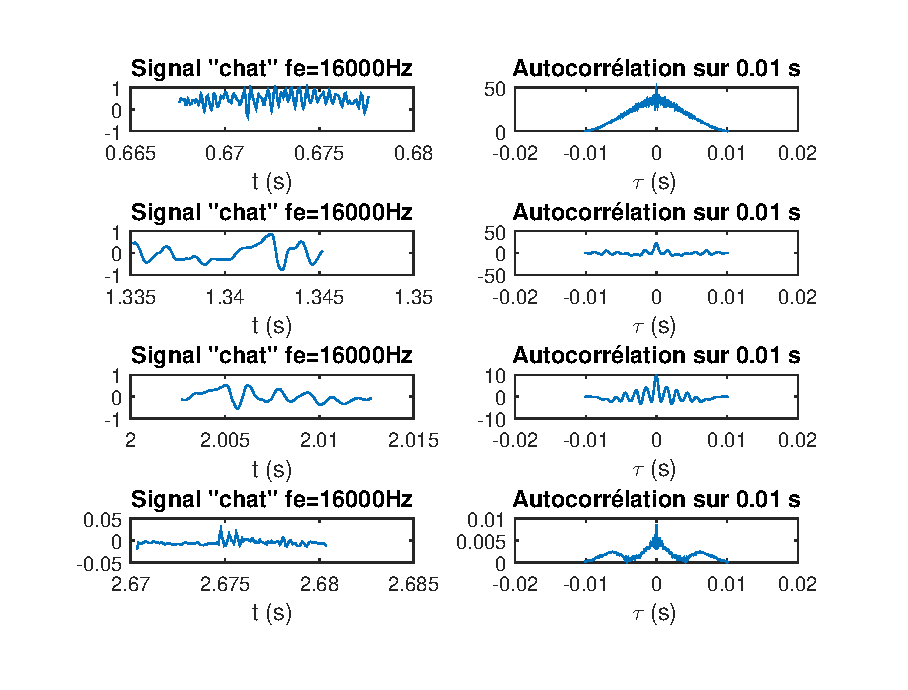
\includegraphics[height=0.45\textheight]{images/classificationVoix1.eps}
\caption{Autocorrélation de divers échantillons du signal vocal.}
\label{classif1}
\end{figure}

La figure \ref{classif1} montre que des échantillons de durée 0.01 secondes sont trop courts pour différencier aisément le signal voisé du non voisé.

\begin{figure}[h!]
\centering
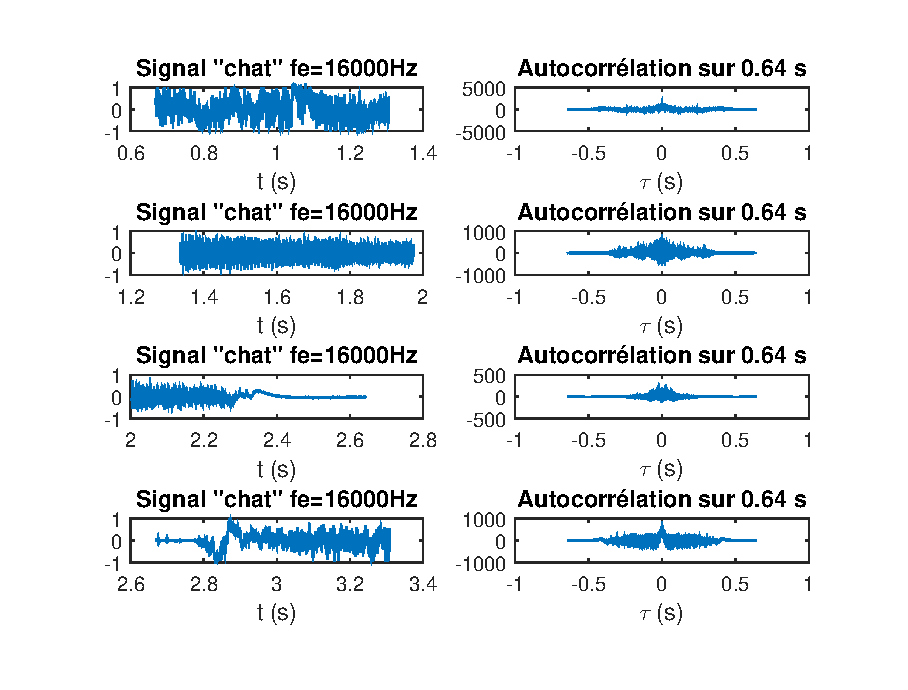
\includegraphics[height=0.45\textheight]{images/classificationVoix4.eps}
\caption{Autocorrélation de divers échantillons du signal vocal.}
\label{classif4}
\end{figure}

La figure \ref{classif4} montre que des échantillons de durée 0.64 secondes sont trop longs. En effet, on se rapproche alors de la période de variation du signal liée au sens de la parole (visible sur l'échantillon pris entre 2 et 2.8 secondes par exemple).


Finalement,  on choisit une durée d'échantillon de 0.16 secondes (figure \ref{classif3}), car bien que celle de 0.06 convienne également pour différencier le signal voisé du non voisé, l'autocorrélation sur une plus grande période fait apparaître plus de maximums locaux, ce qui permet d'estimmer plus précisément la fréquence fondamentale du signal voisé. On trouve ainsi une fréquence du fondamental de 100 Hz environ.

\begin{figure}[h!]
	\centering
	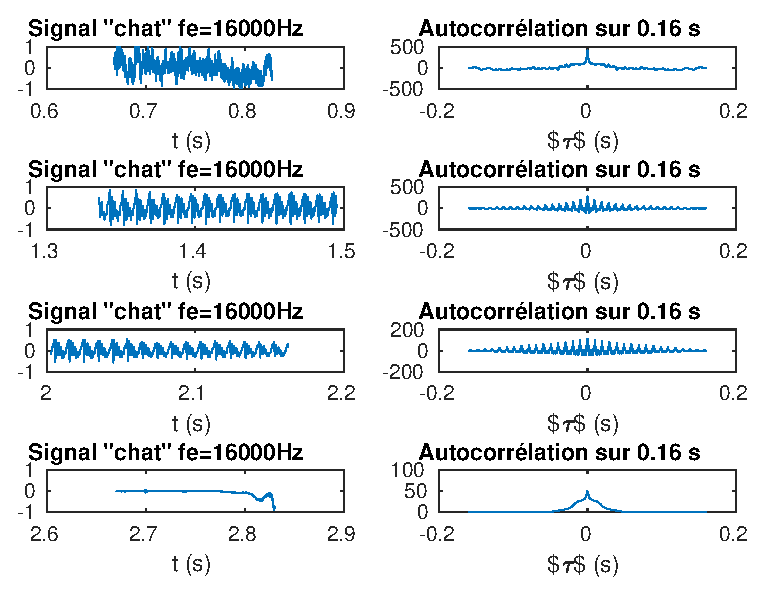
\includegraphics[width=\textwidth]{images/classificationVoix3.eps}
	\caption{Autocorrélation de divers échantillons du signal vocal.}
	\label{classif3}
\end{figure}

\FloatBarrier
\newpage

\part{Aspects fréquentiels}

\section{Échantillonnage}
On réalise l'échantillonage d'un même signal de fréquence $f=500 \; Hz$ échantillonné à plusieurs fréquences différentes, le résultat obtenu est représenté dans les figures \ref{fig:echantillon1}, \ref{fig:echantillon2} et \ref{fig:echantillon3}.

\begin{figure}[h!]
	\centering
	\begin{minipage}{0.45\textwidth}
	\centering
	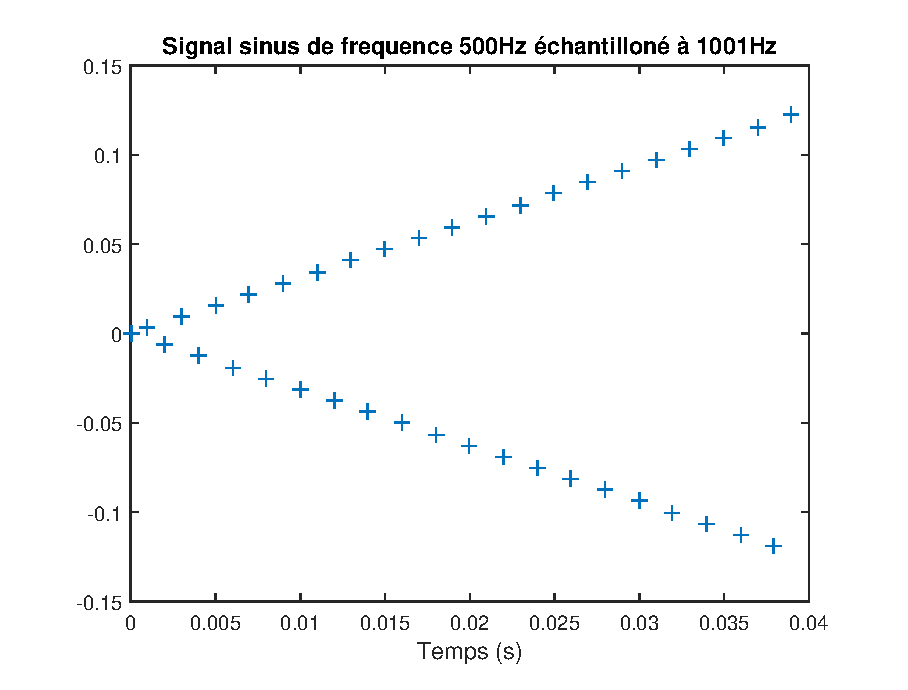
\includegraphics[width=\textwidth]{images/echantillone_1.eps}
	\caption{Signal échantilloné à $2f+1$.}
	\label{fig:echantillon1}

	\end{minipage}
	\begin{minipage}{0.45\textwidth}
	\centering
	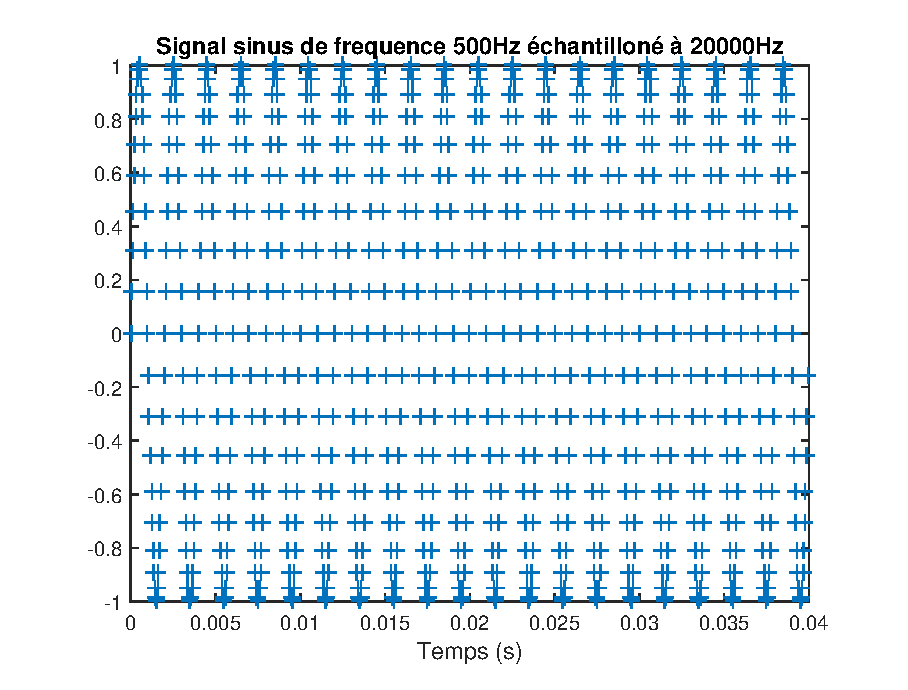
\includegraphics[width=\textwidth]{images/echantillone_2.eps}
	\caption{Signal échantilloné à $40f$.}
	\label{fig:echantillon2}
	\end{minipage}
	\begin{minipage}{0.5\textwidth}
	\centering
	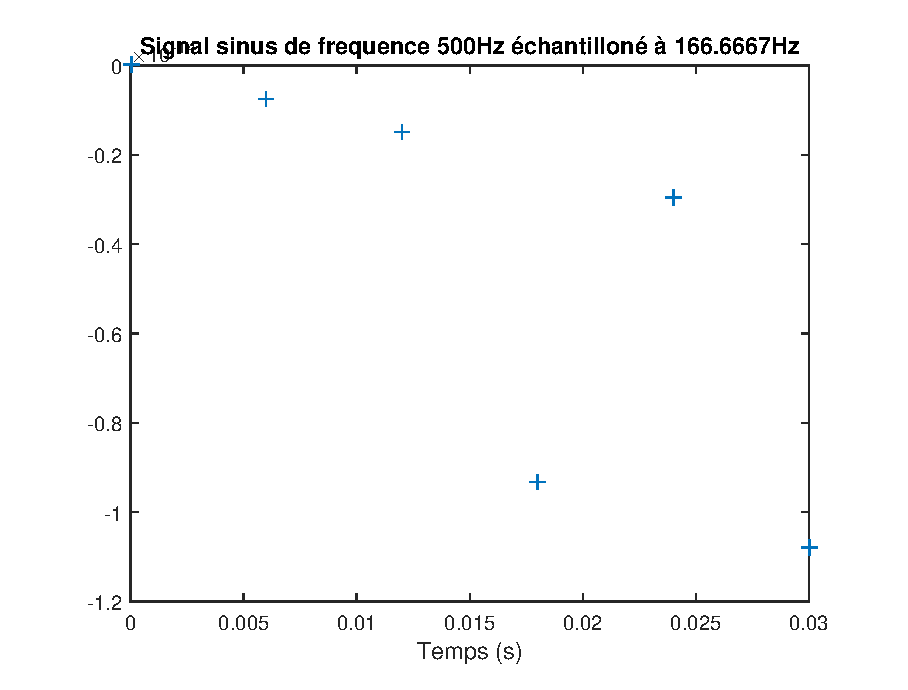
\includegraphics[width=\textwidth]{images/echantillone_3.eps}
	\caption{Signal échantilloné à $\frac{1}{2}f$.}
	\label{fig:echantillon3}
	\end{minipage}
\end{figure}

\FloatBarrier
\section{La Transformée de Fourier discrète (TFD)}

\subsection{Densité spectrale d'énergie}
On trace la densité spectrale d'énergie d'un signal voisé (figure \ref{fig:dse_vois}) et d'un signal non-voisé (figure \ref{fig:dse_nonvois}). On remarque que le signal non voisé ("ch") comporte de l'énergie dans toutes les fréquences de manière identique, tandis que le signal voisé ("a") présente de l'énergie uniquement sur certaines fréquences, ce qui est cohérent avec les résultats obtenus précédemment avec la méthode temporelle. %TODO : Pourquoi c'est cohérent ?


\begin{figure}[h!]
	\centering
	\begin{minipage}{0.45\textwidth}
	\centering
	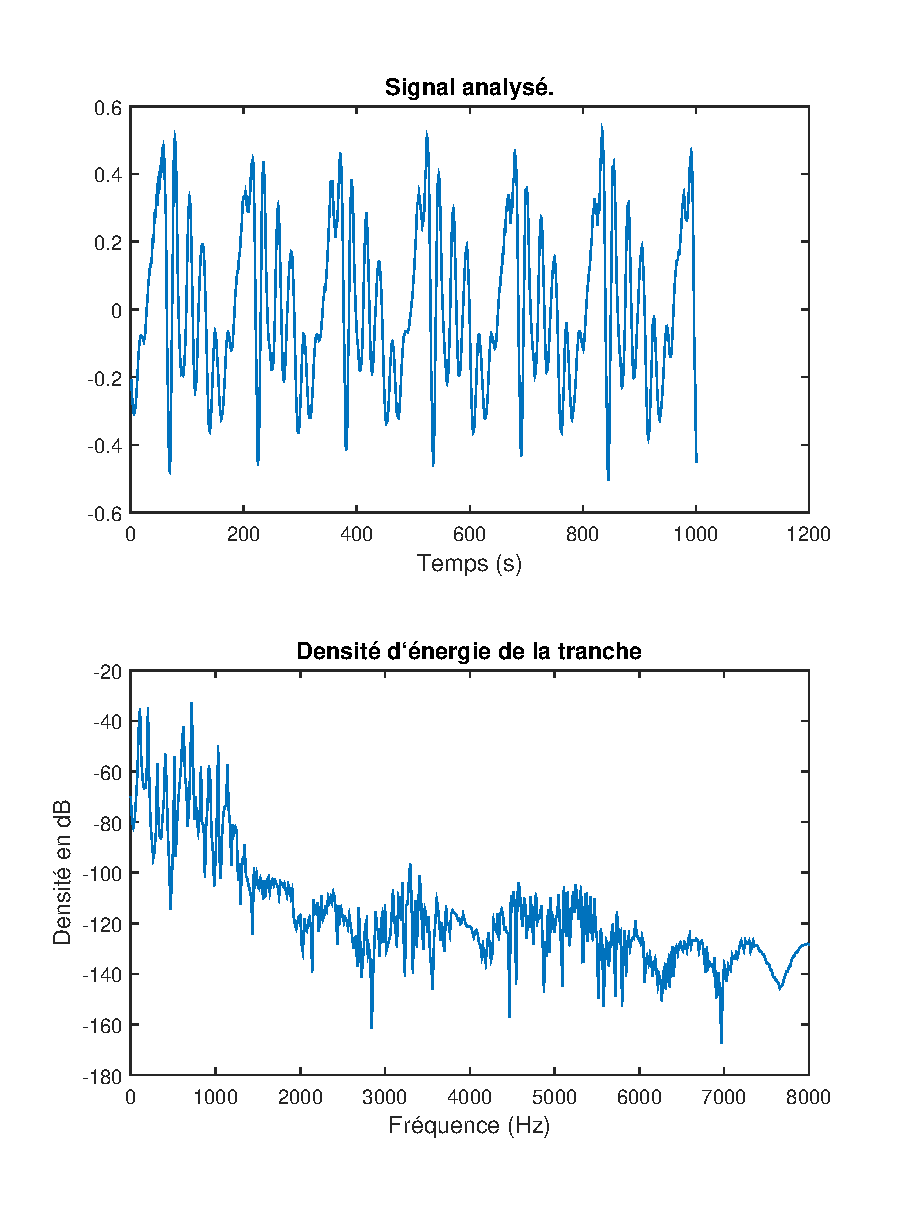
\includegraphics[width=\textwidth]{images/tfd_voise.eps}
	\caption{Signal voisé et \bsc{dse}}
	\label{fig:dse_vois}
	\end{minipage}
	\begin{minipage}{0.45\textwidth}
	\centering
	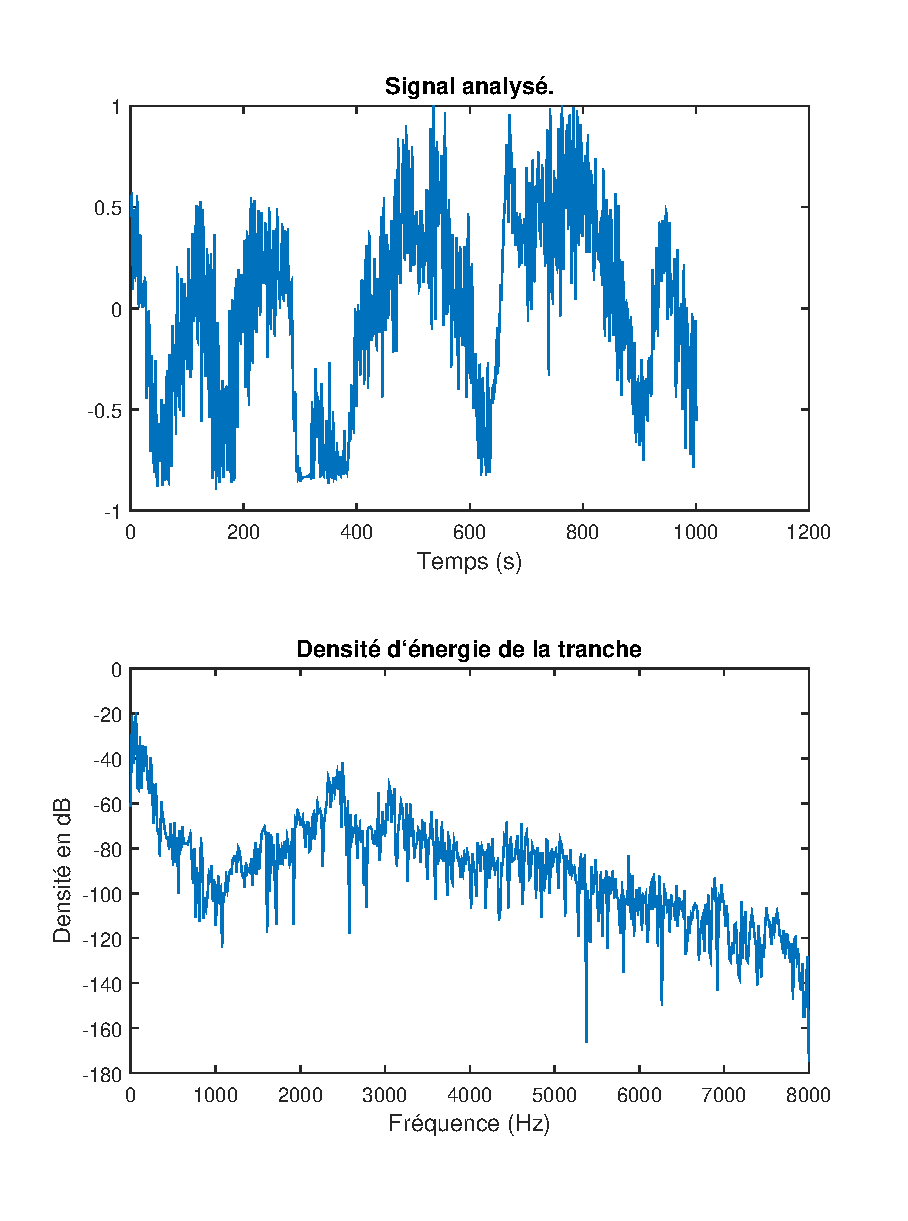
\includegraphics[width=\textwidth]{images/tfd_nonvoise.eps}
	\caption{Signal non-voisé et \bsc{dse}}
	\label{fig:dse_nonvois}
	\end{minipage}
\end{figure}



\FloatBarrier
\subsection{Zéro-padding}
\begin{figure}[h!]
	\centering
	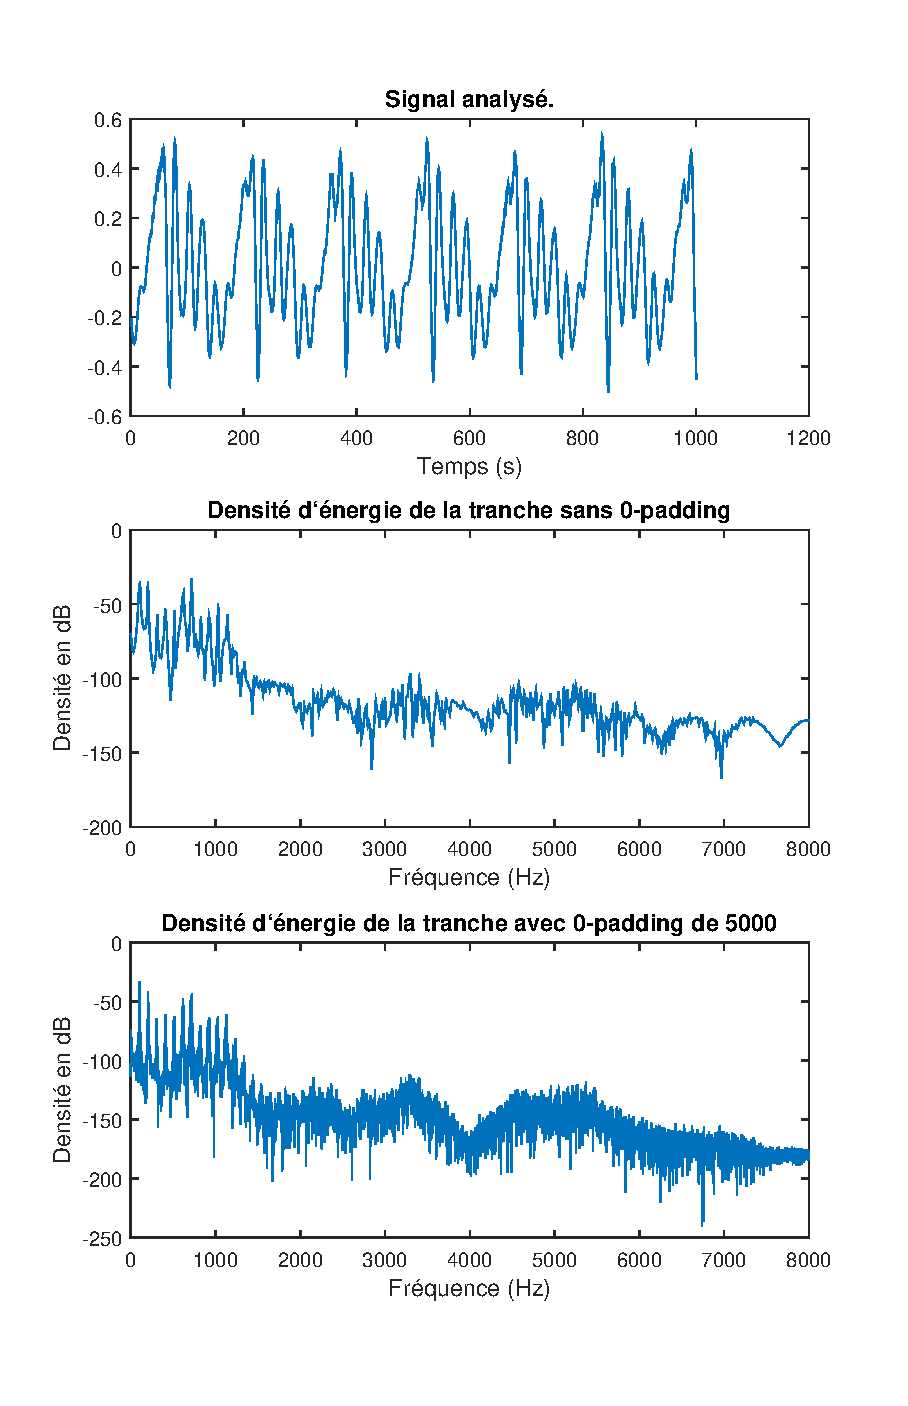
\includegraphics[width=\textwidth]{images/comp_0_padding.eps}
	\caption{Comparaison de la \bsc{dse} avec ou sans 0-padding}
	\label{fig:dse_0_padding}
\end{figure}
On réalise ensuite une fonction de 0-padding. On compare la DSE pour un signal voisé, on se rend compte d'une amélioration de la précision spectrale sans modifier la résolution (l'ajout de zéro n'ajoute pas d'informations dans le spectre, le nombre de point utile reste le même).


\FloatBarrier
\subsection{Réduction/élévation de cadence}

\begin{figure}[h!]
	\centering
	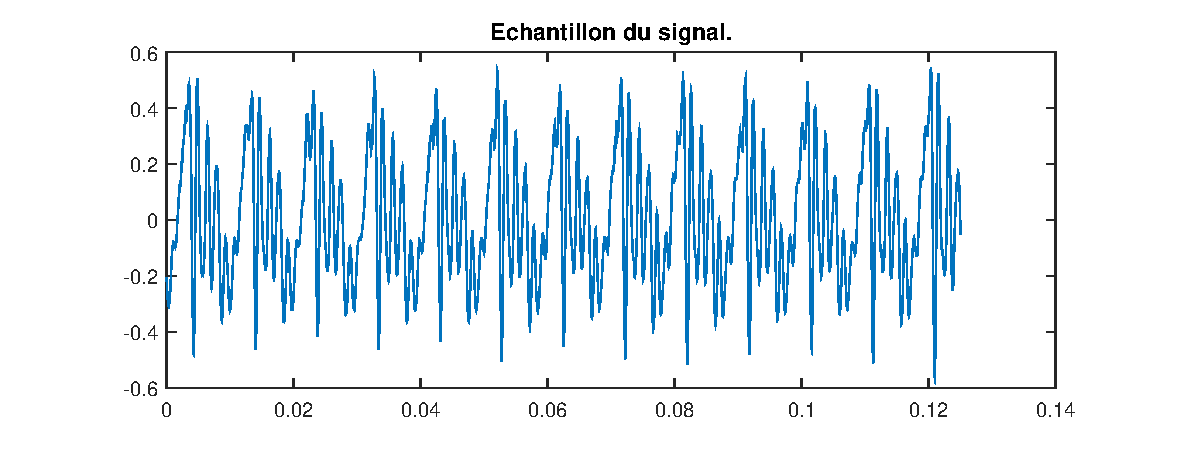
\includegraphics[width=\textwidth]{images/cadence_signal.eps}
	\caption{Signal échantillonné à 16kHz}
	\label{fig:cadence_signal}
\end{figure}

On reprend notre signal ("a") (figure \ref{fig:cadence_signal}) pour évaluer l'influence de l'élévation et de la réduction de cadence.
L'élévation de cadence (figure \ref{fig:élévation}) amène à une fréquence d'échantillonage plus élevée en insérant des zéros entre les intervalles temporels ce qui ajoute des composantes plus aigües à notre signal. La réduction de cadence (figure \ref{fig:réduction}) quant à elle supprime des échantillons et il est possible de ne plus respecter le critère de Shanon, impliquant du repliement spectrale perceptible au travers d'un son en général plus grave.

La fonction 'resample' applqiue un filtre passe bas de manière à supprimer les composantes parasites, le bruit qu'on a en augmentant, diminiuant la cadence ce qui explique pourquoi on a un résultat moins bruité.

\begin{figure}[h!]
\begin{minipage}{0.5\textwidth}
	\centering
	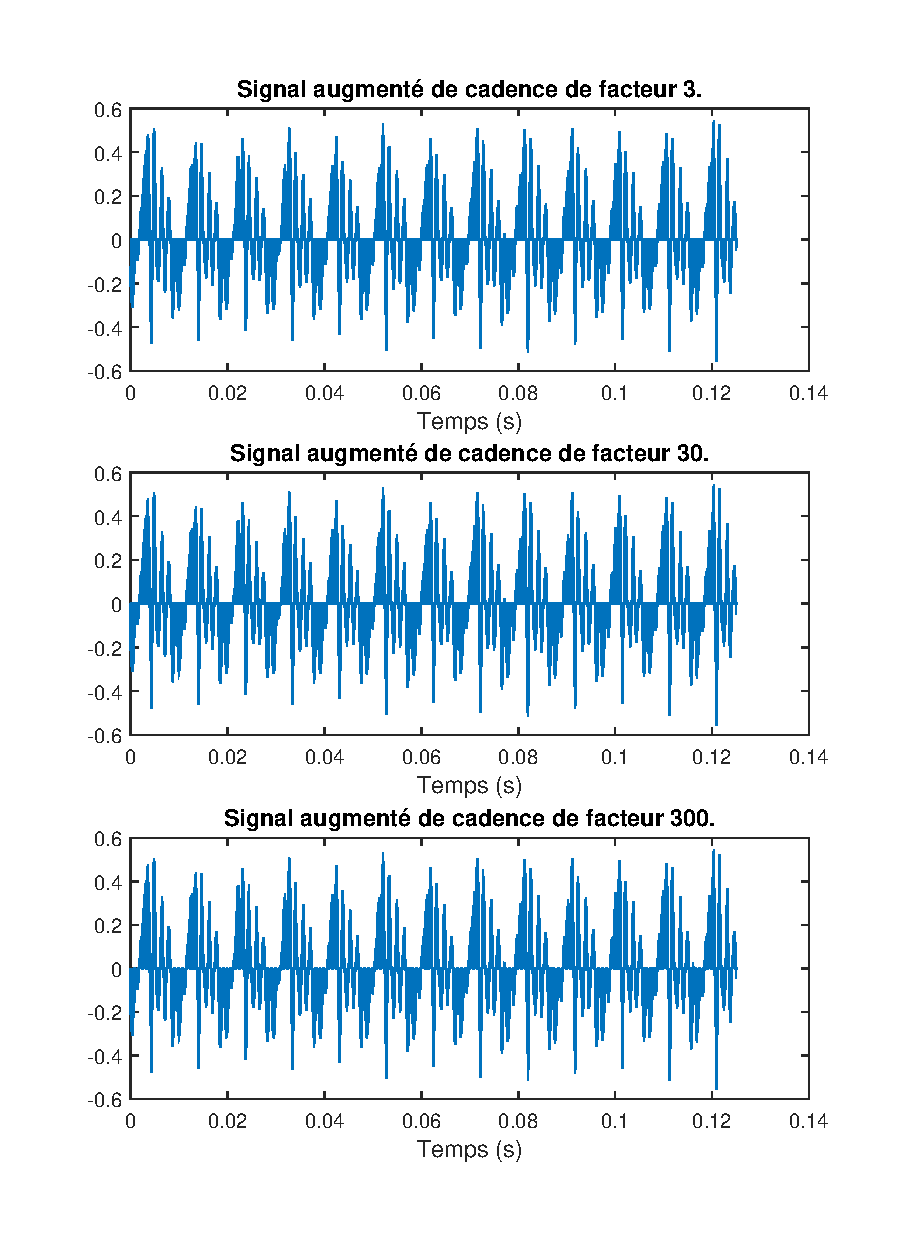
\includegraphics[width=\textwidth]{images/cadence_augmente.eps}
	\caption{Elevation de cadence}
	\label{fig:élévation}
\end{minipage}
\begin{minipage}{0.5\textwidth}
	\centering
	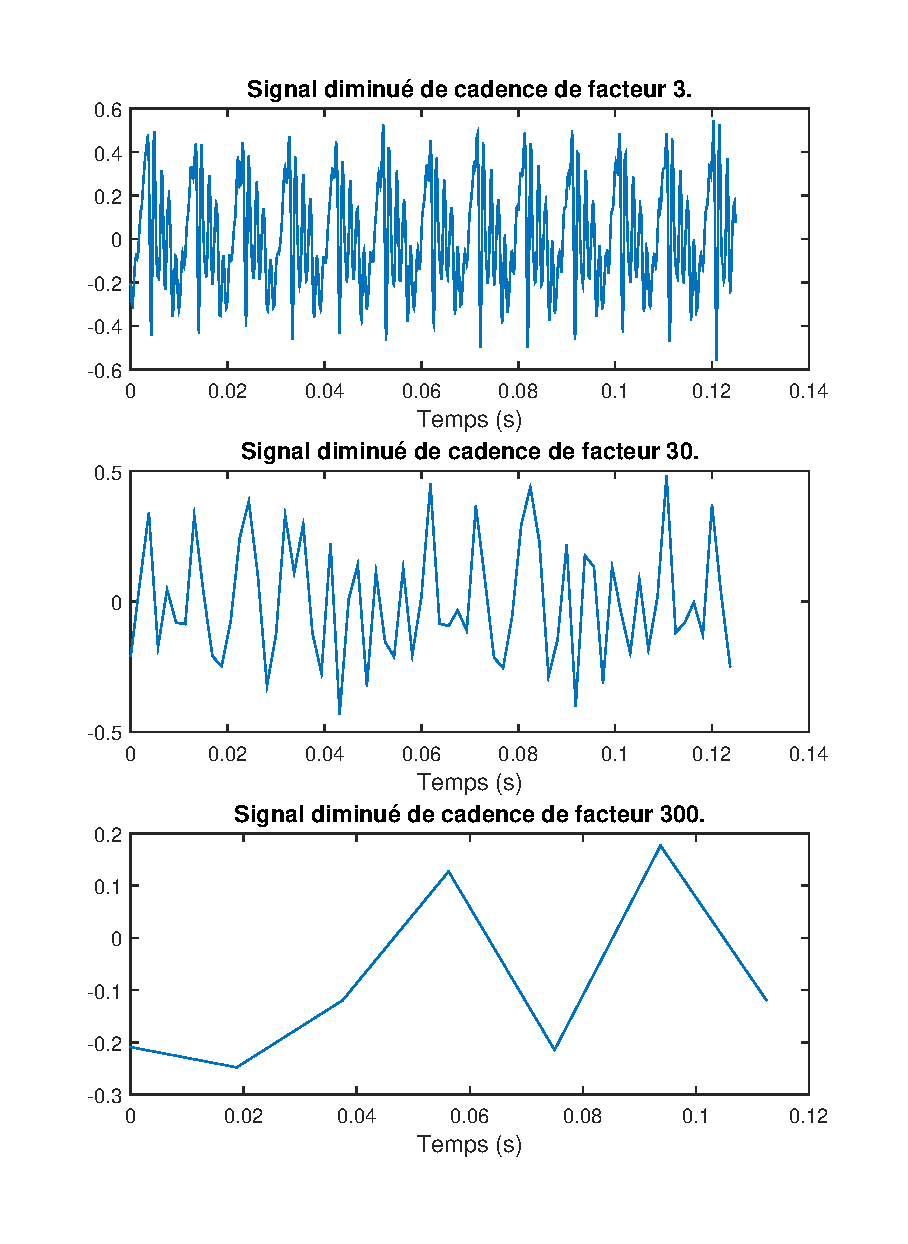
\includegraphics[width=\textwidth]{images/cadence_diminue.eps}
	\caption{Réduction de cadence}
	\label{fig:réduction}
\end{minipage}
\end{figure}

\FloatBarrier
\section{Analyse Spectrale}
\subsection{Analyse d'une tranche de signal par TFD}

La figure \ref{fig:hanning} montre qu'en réalisant la transformée de Fourier de la fenêtre de Hanning, on obtient un triangle de largeur $4/N$
  
\begin{figure}[h!]
	\centering
	\begin{minipage}{0.45\textwidth}
		\centering
		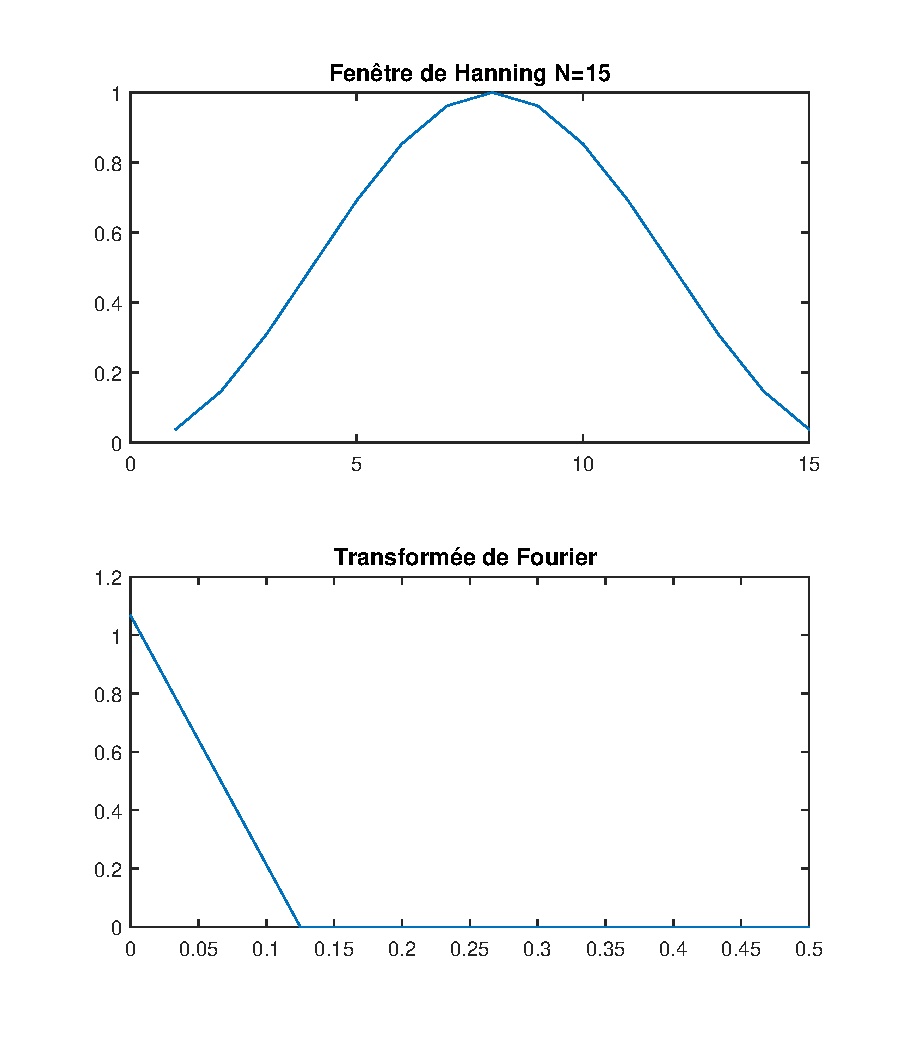
\includegraphics[width=\textwidth]{images/hanning_tfd.eps}
		\caption{TFD d'une fenêtre de Hanning}
		\label{fig:hanning}
	\end{minipage}
	\begin{minipage}{0.45\textwidth}
		\centering
		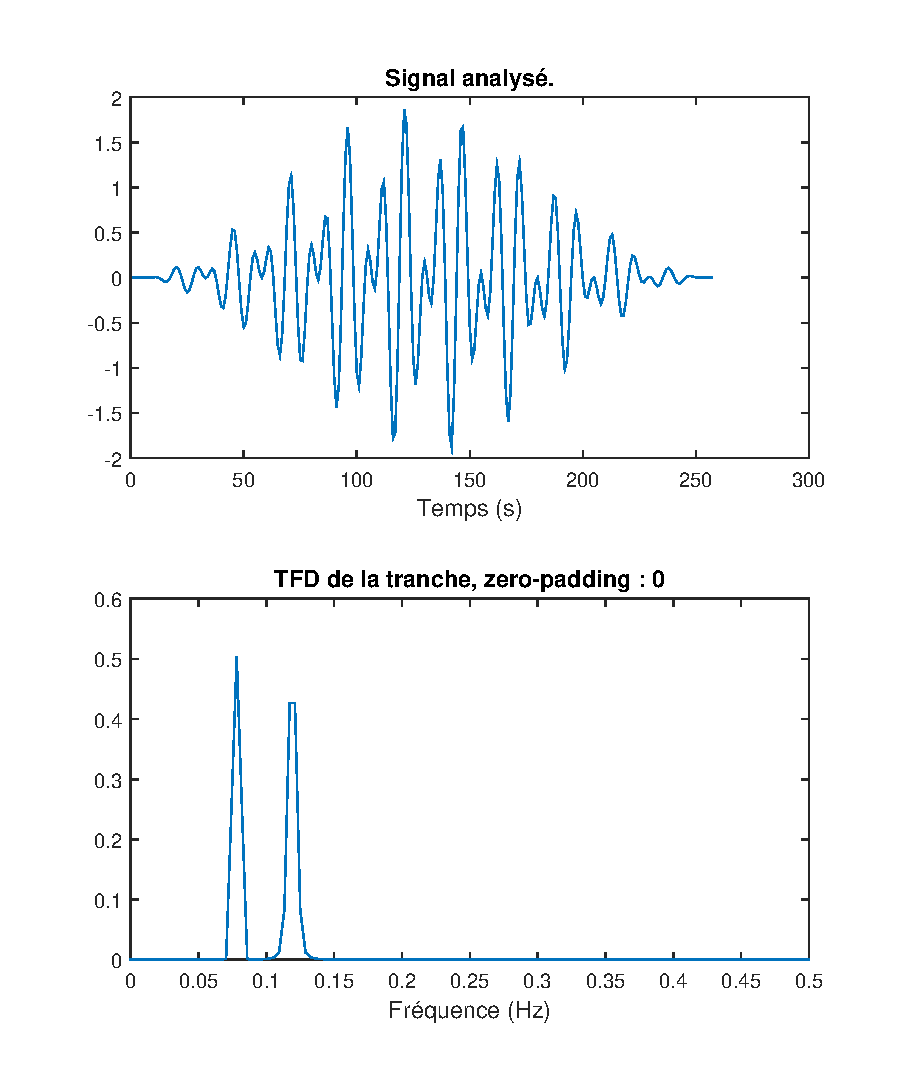
\includegraphics[width=\textwidth]{images/hanning_sans_0p.eps}
		\caption{Analyse d'une somme de cosinus}
		\label{fig:hanning_sans_0p}
	\end{minipage}
\end{figure}

On remarque grâce à la figure \ref{fig:hanning_sans_0p} que du fait de l'échantillonage de la transformée de Fourier, le second pic du graphe est tronqué. On retrouve ainsi le résultat du TD 4.

\subsection{Effets de quelques fenêtres}

Après modification de la fonction d'analyse (voir le fichier \verb`tfd.m`) pour permettre à l'utilisateur de choisir la fenêtre de pondération. On remarque tout d'abord que le 0-padding permet d'augmenter la résolution de la transformée de Fourier discrète. C'est pourquoi on comparera les effets des différentes fenêtres avec un 0-padding de 2048 points.

  
\begin{figure}[h!]
	\centering
	\begin{minipage}{\textwidth}
		\centering
		%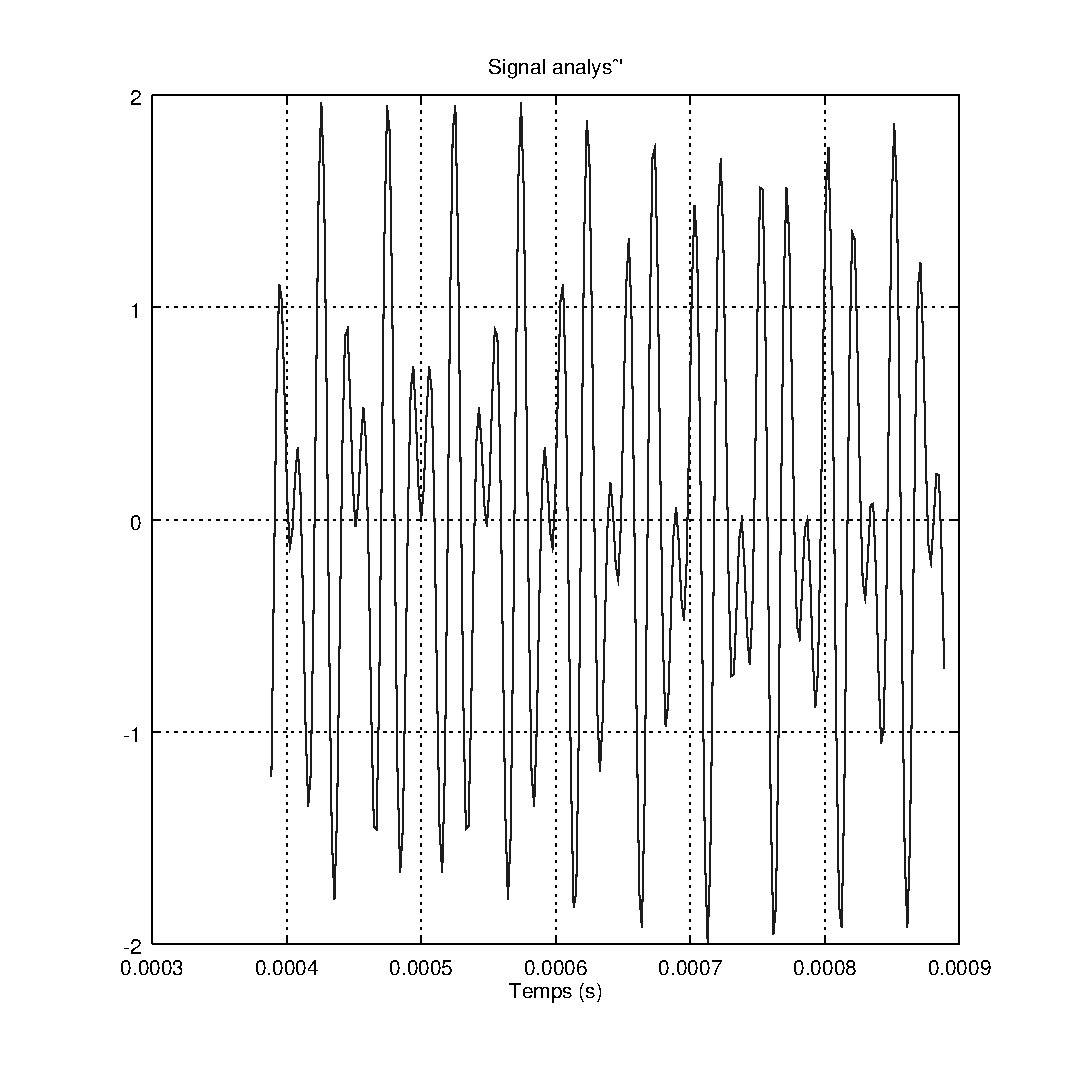
\includegraphics[width=\textwidth]{images/signal_fenetre.eps}
		% Title: glps_renderer figure
% Creator: GL2PS 1.3.8, (C) 1999-2012 C. Geuzaine
% For: Octave
% CreationDate: Wed Nov  8 10:42:42 2017
\begin{pgfpicture}
\pgfsetlinewidth{0.01pt}
\color[rgb]{1.000000,1.000000,1.000000}
\pgfpathmoveto{\pgfpoint{65.000031pt}{104.000000pt}}
\pgflineto{\pgfpoint{452.500000pt}{26.999981pt}}
\pgflineto{\pgfpoint{65.000031pt}{26.999981pt}}
\pgfpathclose
\pgfusepath{fill,stroke}
\pgfpathmoveto{\pgfpoint{65.000031pt}{104.000000pt}}
\pgflineto{\pgfpoint{452.500000pt}{104.000000pt}}
\pgflineto{\pgfpoint{452.500000pt}{26.999981pt}}
\pgfpathclose
\pgfusepath{fill,stroke}
\color[rgb]{0.000000,0.000000,0.000000}
\pgfsetlinewidth{0.500000pt}
\pgfsetdash{{16pt}{0pt}}{0pt}
\pgfpathmoveto{\pgfpoint{452.500000pt}{26.999981pt}}
\pgflineto{\pgfpoint{65.000031pt}{26.999981pt}}
\pgfusepath{stroke}
\pgfpathmoveto{\pgfpoint{452.500000pt}{104.000000pt}}
\pgflineto{\pgfpoint{65.000031pt}{104.000000pt}}
\pgfusepath{stroke}
\pgfpathmoveto{\pgfpoint{65.000031pt}{104.000000pt}}
\pgflineto{\pgfpoint{65.000031pt}{26.999981pt}}
\pgfusepath{stroke}
\pgfpathmoveto{\pgfpoint{452.500000pt}{104.000000pt}}
\pgflineto{\pgfpoint{452.500000pt}{26.999981pt}}
\pgfusepath{stroke}
\pgfsetdash{{0pt}{3pt}{1pt}{3pt}{1pt}{3pt}{1pt}{3pt}{1pt}{0pt}}{0pt}
\pgfpathmoveto{\pgfpoint{65.000031pt}{104.000000pt}}
\pgflineto{\pgfpoint{65.000031pt}{26.999981pt}}
\pgfusepath{stroke}
\pgfpathmoveto{\pgfpoint{129.583359pt}{104.000000pt}}
\pgflineto{\pgfpoint{129.583359pt}{26.999981pt}}
\pgfusepath{stroke}
\pgfpathmoveto{\pgfpoint{194.166718pt}{104.000000pt}}
\pgflineto{\pgfpoint{194.166718pt}{26.999981pt}}
\pgfusepath{stroke}
\pgfpathmoveto{\pgfpoint{258.750061pt}{104.000000pt}}
\pgflineto{\pgfpoint{258.750061pt}{26.999981pt}}
\pgfusepath{stroke}
\pgfpathmoveto{\pgfpoint{323.333344pt}{104.000000pt}}
\pgflineto{\pgfpoint{323.333344pt}{26.999981pt}}
\pgfusepath{stroke}
\pgfpathmoveto{\pgfpoint{387.916718pt}{104.000000pt}}
\pgflineto{\pgfpoint{387.916718pt}{26.999981pt}}
\pgfusepath{stroke}
\pgfpathmoveto{\pgfpoint{452.500000pt}{104.000000pt}}
\pgflineto{\pgfpoint{452.500000pt}{26.999981pt}}
\pgfusepath{stroke}
\pgfsetdash{{16pt}{0pt}}{0pt}
\pgfpathmoveto{\pgfpoint{65.000031pt}{30.874983pt}}
\pgflineto{\pgfpoint{65.000031pt}{26.999981pt}}
\pgfusepath{stroke}
\pgfpathmoveto{\pgfpoint{65.000031pt}{100.125000pt}}
\pgflineto{\pgfpoint{65.000031pt}{104.000000pt}}
\pgfusepath{stroke}
\pgfpathmoveto{\pgfpoint{129.583359pt}{30.874983pt}}
\pgflineto{\pgfpoint{129.583359pt}{26.999981pt}}
\pgfusepath{stroke}
\pgfpathmoveto{\pgfpoint{129.583359pt}{100.125000pt}}
\pgflineto{\pgfpoint{129.583359pt}{104.000000pt}}
\pgfusepath{stroke}
\pgfpathmoveto{\pgfpoint{194.166718pt}{30.874983pt}}
\pgflineto{\pgfpoint{194.166718pt}{26.999981pt}}
\pgfusepath{stroke}
\pgfpathmoveto{\pgfpoint{194.166718pt}{100.125000pt}}
\pgflineto{\pgfpoint{194.166718pt}{104.000000pt}}
\pgfusepath{stroke}
\pgfpathmoveto{\pgfpoint{258.750061pt}{30.874983pt}}
\pgflineto{\pgfpoint{258.750061pt}{26.999981pt}}
\pgfusepath{stroke}
\pgfpathmoveto{\pgfpoint{258.750061pt}{100.125000pt}}
\pgflineto{\pgfpoint{258.750061pt}{104.000000pt}}
\pgfusepath{stroke}
\pgfpathmoveto{\pgfpoint{323.333344pt}{30.874983pt}}
\pgflineto{\pgfpoint{323.333344pt}{26.999981pt}}
\pgfusepath{stroke}
\pgfpathmoveto{\pgfpoint{323.333344pt}{100.125000pt}}
\pgflineto{\pgfpoint{323.333344pt}{104.000000pt}}
\pgfusepath{stroke}
\pgfpathmoveto{\pgfpoint{387.916718pt}{30.874983pt}}
\pgflineto{\pgfpoint{387.916718pt}{26.999981pt}}
\pgfusepath{stroke}
\pgfpathmoveto{\pgfpoint{387.916718pt}{100.125000pt}}
\pgflineto{\pgfpoint{387.916718pt}{104.000000pt}}
\pgfusepath{stroke}
\pgfpathmoveto{\pgfpoint{452.500000pt}{30.874983pt}}
\pgflineto{\pgfpoint{452.500000pt}{26.999981pt}}
\pgfusepath{stroke}
\pgfpathmoveto{\pgfpoint{452.500000pt}{100.125000pt}}
\pgflineto{\pgfpoint{452.500000pt}{104.000000pt}}
\pgfusepath{stroke}
{
\pgftransformshift{\pgfpoint{65.000015pt}{21.999977pt}}
\pgfnode{rectangle}{north}{\fontsize{10}{0}\selectfont\textcolor[rgb]{0,0,0}{{0.0003}}}{}{\pgfusepath{discard}}}
{
\pgftransformshift{\pgfpoint{129.583328pt}{21.999977pt}}
\pgfnode{rectangle}{north}{\fontsize{10}{0}\selectfont\textcolor[rgb]{0,0,0}{{0.0004}}}{}{\pgfusepath{discard}}}
{
\pgftransformshift{\pgfpoint{194.166702pt}{21.999977pt}}
\pgfnode{rectangle}{north}{\fontsize{10}{0}\selectfont\textcolor[rgb]{0,0,0}{{0.0005}}}{}{\pgfusepath{discard}}}
{
\pgftransformshift{\pgfpoint{258.750031pt}{21.999977pt}}
\pgfnode{rectangle}{north}{\fontsize{10}{0}\selectfont\textcolor[rgb]{0,0,0}{{0.0006}}}{}{\pgfusepath{discard}}}
{
\pgftransformshift{\pgfpoint{323.333344pt}{21.999977pt}}
\pgfnode{rectangle}{north}{\fontsize{10}{0}\selectfont\textcolor[rgb]{0,0,0}{{0.0007}}}{}{\pgfusepath{discard}}}
{
\pgftransformshift{\pgfpoint{387.916687pt}{21.999977pt}}
\pgfnode{rectangle}{north}{\fontsize{10}{0}\selectfont\textcolor[rgb]{0,0,0}{{0.0008}}}{}{\pgfusepath{discard}}}
{
\pgftransformshift{\pgfpoint{452.500000pt}{21.999977pt}}
\pgfnode{rectangle}{north}{\fontsize{10}{0}\selectfont\textcolor[rgb]{0,0,0}{{0.0009}}}{}{\pgfusepath{discard}}}
\pgfsetdash{{0pt}{3pt}{1pt}{3pt}{1pt}{3pt}{1pt}{3pt}{1pt}{0pt}}{0pt}
\pgfpathmoveto{\pgfpoint{452.500000pt}{26.999981pt}}
\pgflineto{\pgfpoint{65.000031pt}{26.999981pt}}
\pgfusepath{stroke}
\pgfpathmoveto{\pgfpoint{452.500000pt}{46.249985pt}}
\pgflineto{\pgfpoint{65.000031pt}{46.249985pt}}
\pgfusepath{stroke}
\pgfpathmoveto{\pgfpoint{452.500000pt}{65.499992pt}}
\pgflineto{\pgfpoint{65.000031pt}{65.499992pt}}
\pgfusepath{stroke}
\pgfpathmoveto{\pgfpoint{452.500000pt}{84.750000pt}}
\pgflineto{\pgfpoint{65.000031pt}{84.750000pt}}
\pgfusepath{stroke}
\pgfpathmoveto{\pgfpoint{452.500000pt}{104.000000pt}}
\pgflineto{\pgfpoint{65.000031pt}{104.000000pt}}
\pgfusepath{stroke}
\pgfsetdash{{16pt}{0pt}}{0pt}
\pgfpathmoveto{\pgfpoint{68.870026pt}{26.999981pt}}
\pgflineto{\pgfpoint{65.000031pt}{26.999981pt}}
\pgfusepath{stroke}
\pgfpathmoveto{\pgfpoint{448.630066pt}{26.999981pt}}
\pgflineto{\pgfpoint{452.500000pt}{26.999981pt}}
\pgfusepath{stroke}
\pgfpathmoveto{\pgfpoint{68.870026pt}{46.249985pt}}
\pgflineto{\pgfpoint{65.000031pt}{46.249985pt}}
\pgfusepath{stroke}
\pgfpathmoveto{\pgfpoint{448.630066pt}{46.249985pt}}
\pgflineto{\pgfpoint{452.500000pt}{46.249985pt}}
\pgfusepath{stroke}
\pgfpathmoveto{\pgfpoint{68.870026pt}{65.499992pt}}
\pgflineto{\pgfpoint{65.000031pt}{65.499992pt}}
\pgfusepath{stroke}
\pgfpathmoveto{\pgfpoint{448.630066pt}{65.499992pt}}
\pgflineto{\pgfpoint{452.500000pt}{65.499992pt}}
\pgfusepath{stroke}
\pgfpathmoveto{\pgfpoint{68.870026pt}{84.750000pt}}
\pgflineto{\pgfpoint{65.000031pt}{84.750000pt}}
\pgfusepath{stroke}
\pgfpathmoveto{\pgfpoint{448.630066pt}{84.750000pt}}
\pgflineto{\pgfpoint{452.500000pt}{84.750000pt}}
\pgfusepath{stroke}
\pgfpathmoveto{\pgfpoint{68.870026pt}{104.000000pt}}
\pgflineto{\pgfpoint{65.000031pt}{104.000000pt}}
\pgfusepath{stroke}
\pgfpathmoveto{\pgfpoint{448.630066pt}{104.000000pt}}
\pgflineto{\pgfpoint{452.500000pt}{104.000000pt}}
\pgfusepath{stroke}
{
\pgftransformshift{\pgfpoint{60.006439pt}{26.999981pt}}
\pgfnode{rectangle}{east}{\fontsize{10}{0}\selectfont\textcolor[rgb]{0,0,0}{{-2}}}{}{\pgfusepath{discard}}}
{
\pgftransformshift{\pgfpoint{60.006439pt}{46.249985pt}}
\pgfnode{rectangle}{east}{\fontsize{10}{0}\selectfont\textcolor[rgb]{0,0,0}{{-1}}}{}{\pgfusepath{discard}}}
{
\pgftransformshift{\pgfpoint{60.006439pt}{65.499992pt}}
\pgfnode{rectangle}{east}{\fontsize{10}{0}\selectfont\textcolor[rgb]{0,0,0}{{0}}}{}{\pgfusepath{discard}}}
{
\pgftransformshift{\pgfpoint{60.006439pt}{84.750000pt}}
\pgfnode{rectangle}{east}{\fontsize{10}{0}\selectfont\textcolor[rgb]{0,0,0}{{1}}}{}{\pgfusepath{discard}}}
{
\pgftransformshift{\pgfpoint{60.006439pt}{104.000000pt}}
\pgfnode{rectangle}{east}{\fontsize{10}{0}\selectfont\textcolor[rgb]{0,0,0}{{2}}}{}{\pgfusepath{discard}}}
{
\pgftransformshift{\pgfpoint{258.750031pt}{10.999977pt}}
\pgfnode{rectangle}{north}{\fontsize{10}{0}\selectfont\textcolor[rgb]{0,0,0}{{Temps (s)}}}{}{\pgfusepath{discard}}}
\color[rgb]{0.000000,0.000000,1.000000}
\pgfsetdash{}{0pt}
\pgfpathmoveto{\pgfpoint{123.528656pt}{60.962570pt}}
\pgflineto{\pgfpoint{122.267273pt}{42.172722pt}}
\pgfusepath{stroke}
\pgfpathmoveto{\pgfpoint{124.790070pt}{78.114960pt}}
\pgflineto{\pgfpoint{123.528656pt}{60.962570pt}}
\pgfusepath{stroke}
\pgfpathmoveto{\pgfpoint{126.051453pt}{86.854027pt}}
\pgflineto{\pgfpoint{124.790070pt}{78.114960pt}}
\pgfusepath{stroke}
\pgfpathmoveto{\pgfpoint{127.312836pt}{85.296417pt}}
\pgflineto{\pgfpoint{126.051453pt}{86.854027pt}}
\pgfusepath{stroke}
\pgfpathmoveto{\pgfpoint{128.574219pt}{76.799545pt}}
\pgflineto{\pgfpoint{127.312836pt}{85.296417pt}}
\pgfusepath{stroke}
\pgfpathmoveto{\pgfpoint{129.835632pt}{67.570236pt}}
\pgflineto{\pgfpoint{128.574219pt}{76.799545pt}}
\pgfusepath{stroke}
\pgfpathmoveto{\pgfpoint{131.097015pt}{62.953091pt}}
\pgflineto{\pgfpoint{129.835632pt}{67.570236pt}}
\pgfusepath{stroke}
\pgfpathmoveto{\pgfpoint{132.358429pt}{64.476028pt}}
\pgflineto{\pgfpoint{131.097015pt}{62.953091pt}}
\pgfusepath{stroke}
\pgfpathmoveto{\pgfpoint{133.619812pt}{69.255478pt}}
\pgflineto{\pgfpoint{132.358429pt}{64.476028pt}}
\pgfusepath{stroke}
\pgfpathmoveto{\pgfpoint{134.881195pt}{72.026909pt}}
\pgflineto{\pgfpoint{133.619812pt}{69.255478pt}}
\pgfusepath{stroke}
\pgfpathmoveto{\pgfpoint{136.142578pt}{68.599434pt}}
\pgflineto{\pgfpoint{134.881195pt}{72.026909pt}}
\pgfusepath{stroke}
\pgfpathmoveto{\pgfpoint{137.403992pt}{58.736439pt}}
\pgflineto{\pgfpoint{136.142578pt}{68.599434pt}}
\pgfusepath{stroke}
\pgfpathmoveto{\pgfpoint{138.665375pt}{46.770752pt}}
\pgflineto{\pgfpoint{137.403992pt}{58.736439pt}}
\pgfusepath{stroke}
\pgfpathmoveto{\pgfpoint{139.926788pt}{39.510094pt}}
\pgflineto{\pgfpoint{138.665375pt}{46.770752pt}}
\pgfusepath{stroke}
\pgfpathmoveto{\pgfpoint{141.188171pt}{42.500294pt}}
\pgflineto{\pgfpoint{139.926788pt}{39.510094pt}}
\pgfusepath{stroke}
\pgfpathmoveto{\pgfpoint{142.449554pt}{56.667091pt}}
\pgflineto{\pgfpoint{141.188171pt}{42.500294pt}}
\pgfusepath{stroke}
\pgfpathmoveto{\pgfpoint{143.710968pt}{77.224968pt}}
\pgflineto{\pgfpoint{142.449554pt}{56.667091pt}}
\pgfusepath{stroke}
\pgfpathmoveto{\pgfpoint{144.972351pt}{95.577187pt}}
\pgflineto{\pgfpoint{143.710968pt}{77.224968pt}}
\pgfusepath{stroke}
\pgfpathmoveto{\pgfpoint{146.233734pt}{103.346710pt}}
\pgflineto{\pgfpoint{144.972351pt}{95.577187pt}}
\pgfusepath{stroke}
\pgfpathmoveto{\pgfpoint{147.495117pt}{96.516273pt}}
\pgflineto{\pgfpoint{146.233734pt}{103.346710pt}}
\pgfusepath{stroke}
\pgfpathmoveto{\pgfpoint{148.756531pt}{77.544022pt}}
\pgflineto{\pgfpoint{147.495117pt}{96.516273pt}}
\pgfusepath{stroke}
\pgfpathmoveto{\pgfpoint{150.017914pt}{54.331120pt}}
\pgflineto{\pgfpoint{148.756531pt}{77.544022pt}}
\pgfusepath{stroke}
\pgfpathmoveto{\pgfpoint{151.279327pt}{36.526840pt}}
\pgflineto{\pgfpoint{150.017914pt}{54.331120pt}}
\pgfusepath{stroke}
\pgfpathmoveto{\pgfpoint{152.540710pt}{31.021513pt}}
\pgflineto{\pgfpoint{151.279327pt}{36.526840pt}}
\pgfusepath{stroke}
\pgfpathmoveto{\pgfpoint{153.802124pt}{38.883327pt}}
\pgflineto{\pgfpoint{152.540710pt}{31.021513pt}}
\pgfusepath{stroke}
\pgfpathmoveto{\pgfpoint{155.063477pt}{55.230064pt}}
\pgflineto{\pgfpoint{153.802124pt}{38.883327pt}}
\pgfusepath{stroke}
\pgfpathmoveto{\pgfpoint{156.324890pt}{71.999832pt}}
\pgflineto{\pgfpoint{155.063477pt}{55.230064pt}}
\pgfusepath{stroke}
\pgfpathmoveto{\pgfpoint{157.586273pt}{82.101456pt}}
\pgflineto{\pgfpoint{156.324890pt}{71.999832pt}}
\pgfusepath{stroke}
\pgfpathmoveto{\pgfpoint{158.847687pt}{82.763130pt}}
\pgflineto{\pgfpoint{157.586273pt}{82.101456pt}}
\pgfusepath{stroke}
\pgfpathmoveto{\pgfpoint{160.109070pt}{76.393555pt}}
\pgflineto{\pgfpoint{158.847687pt}{82.763130pt}}
\pgfusepath{stroke}
\pgfpathmoveto{\pgfpoint{161.370453pt}{68.641602pt}}
\pgflineto{\pgfpoint{160.109070pt}{76.393555pt}}
\pgfusepath{stroke}
\pgfpathmoveto{\pgfpoint{162.631866pt}{64.846214pt}}
\pgflineto{\pgfpoint{161.370453pt}{68.641602pt}}
\pgfusepath{stroke}
\pgfpathmoveto{\pgfpoint{163.893250pt}{66.899727pt}}
\pgflineto{\pgfpoint{162.631866pt}{64.846214pt}}
\pgfusepath{stroke}
\pgfpathmoveto{\pgfpoint{165.154633pt}{72.268394pt}}
\pgflineto{\pgfpoint{163.893250pt}{66.899727pt}}
\pgfusepath{stroke}
\pgfpathmoveto{\pgfpoint{166.416046pt}{75.686264pt}}
\pgflineto{\pgfpoint{165.154633pt}{72.268394pt}}
\pgfusepath{stroke}
\pgfpathmoveto{\pgfpoint{167.677429pt}{72.536469pt}}
\pgflineto{\pgfpoint{166.416046pt}{75.686264pt}}
\pgfusepath{stroke}
\pgfpathmoveto{\pgfpoint{168.938812pt}{61.978619pt}}
\pgflineto{\pgfpoint{167.677429pt}{72.536469pt}}
\pgfusepath{stroke}
\pgfpathmoveto{\pgfpoint{170.200226pt}{47.994278pt}}
\pgflineto{\pgfpoint{168.938812pt}{61.978619pt}}
\pgfusepath{stroke}
\pgfpathmoveto{\pgfpoint{171.461609pt}{37.650986pt}}
\pgflineto{\pgfpoint{170.200226pt}{47.994278pt}}
\pgfusepath{stroke}
\pgfpathmoveto{\pgfpoint{172.722992pt}{37.420044pt}}
\pgflineto{\pgfpoint{171.461609pt}{37.650986pt}}
\pgfusepath{stroke}
\pgfpathmoveto{\pgfpoint{173.984375pt}{49.494198pt}}
\pgflineto{\pgfpoint{172.722992pt}{37.420044pt}}
\pgfusepath{stroke}
\pgfpathmoveto{\pgfpoint{175.245789pt}{70.126511pt}}
\pgflineto{\pgfpoint{173.984375pt}{49.494198pt}}
\pgfusepath{stroke}
\pgfpathmoveto{\pgfpoint{176.507172pt}{90.994080pt}}
\pgflineto{\pgfpoint{175.245789pt}{70.126511pt}}
\pgfusepath{stroke}
\pgfpathmoveto{\pgfpoint{177.768585pt}{103.008453pt}}
\pgflineto{\pgfpoint{176.507172pt}{90.994080pt}}
\pgfusepath{stroke}
\pgfpathmoveto{\pgfpoint{179.029968pt}{100.686478pt}}
\pgflineto{\pgfpoint{177.768585pt}{103.008453pt}}
\pgfusepath{stroke}
\pgfpathmoveto{\pgfpoint{180.291382pt}{84.859924pt}}
\pgflineto{\pgfpoint{179.029968pt}{100.686478pt}}
\pgfusepath{stroke}
\pgfpathmoveto{\pgfpoint{181.552765pt}{62.327499pt}}
\pgflineto{\pgfpoint{180.291382pt}{84.859924pt}}
\pgfusepath{stroke}
\pgfpathmoveto{\pgfpoint{182.814148pt}{42.612518pt}}
\pgflineto{\pgfpoint{181.552765pt}{62.327499pt}}
\pgfusepath{stroke}
\pgfpathmoveto{\pgfpoint{184.075531pt}{33.467079pt}}
\pgflineto{\pgfpoint{182.814148pt}{42.612518pt}}
\pgfusepath{stroke}
\pgfpathmoveto{\pgfpoint{185.336945pt}{37.385769pt}}
\pgflineto{\pgfpoint{184.075531pt}{33.467079pt}}
\pgfusepath{stroke}
\pgfpathmoveto{\pgfpoint{186.598328pt}{50.837570pt}}
\pgflineto{\pgfpoint{185.336945pt}{37.385769pt}}
\pgfusepath{stroke}
\pgfpathmoveto{\pgfpoint{187.859711pt}{66.492882pt}}
\pgflineto{\pgfpoint{186.598328pt}{50.837570pt}}
\pgfusepath{stroke}
\pgfpathmoveto{\pgfpoint{189.121124pt}{77.174988pt}}
\pgflineto{\pgfpoint{187.859711pt}{66.492882pt}}
\pgfusepath{stroke}
\pgfpathmoveto{\pgfpoint{190.382507pt}{79.415367pt}}
\pgflineto{\pgfpoint{189.121124pt}{77.174988pt}}
\pgfusepath{stroke}
\pgfpathmoveto{\pgfpoint{191.643921pt}{74.778603pt}}
\pgflineto{\pgfpoint{190.382507pt}{79.415367pt}}
\pgfusepath{stroke}
\pgfpathmoveto{\pgfpoint{192.905273pt}{68.373383pt}}
\pgflineto{\pgfpoint{191.643921pt}{74.778603pt}}
\pgfusepath{stroke}
\pgfpathmoveto{\pgfpoint{194.166718pt}{65.499992pt}}
\pgflineto{\pgfpoint{192.905273pt}{68.373383pt}}
\pgfusepath{stroke}
\pgfpathmoveto{\pgfpoint{195.428070pt}{68.373383pt}}
\pgflineto{\pgfpoint{194.166718pt}{65.499992pt}}
\pgfusepath{stroke}
\pgfpathmoveto{\pgfpoint{196.689453pt}{74.778603pt}}
\pgflineto{\pgfpoint{195.428070pt}{68.373383pt}}
\pgfusepath{stroke}
\pgfpathmoveto{\pgfpoint{197.950867pt}{79.415367pt}}
\pgflineto{\pgfpoint{196.689453pt}{74.778603pt}}
\pgfusepath{stroke}
\pgfpathmoveto{\pgfpoint{199.212250pt}{77.174988pt}}
\pgflineto{\pgfpoint{197.950867pt}{79.415367pt}}
\pgfusepath{stroke}
\pgfpathmoveto{\pgfpoint{200.473663pt}{66.492882pt}}
\pgflineto{\pgfpoint{199.212250pt}{77.174988pt}}
\pgfusepath{stroke}
\pgfpathmoveto{\pgfpoint{201.735046pt}{50.837570pt}}
\pgflineto{\pgfpoint{200.473663pt}{66.492882pt}}
\pgfusepath{stroke}
\pgfpathmoveto{\pgfpoint{202.996460pt}{37.385769pt}}
\pgflineto{\pgfpoint{201.735046pt}{50.837570pt}}
\pgfusepath{stroke}
\pgfpathmoveto{\pgfpoint{204.257843pt}{33.467079pt}}
\pgflineto{\pgfpoint{202.996460pt}{37.385769pt}}
\pgfusepath{stroke}
\pgfpathmoveto{\pgfpoint{205.519196pt}{42.612518pt}}
\pgflineto{\pgfpoint{204.257843pt}{33.467079pt}}
\pgfusepath{stroke}
\pgfpathmoveto{\pgfpoint{206.780609pt}{62.327499pt}}
\pgflineto{\pgfpoint{205.519196pt}{42.612518pt}}
\pgfusepath{stroke}
\pgfpathmoveto{\pgfpoint{208.041992pt}{84.859924pt}}
\pgflineto{\pgfpoint{206.780609pt}{62.327499pt}}
\pgfusepath{stroke}
\pgfpathmoveto{\pgfpoint{209.303406pt}{100.686478pt}}
\pgflineto{\pgfpoint{208.041992pt}{84.859924pt}}
\pgfusepath{stroke}
\pgfpathmoveto{\pgfpoint{210.564789pt}{103.008453pt}}
\pgflineto{\pgfpoint{209.303406pt}{100.686478pt}}
\pgfusepath{stroke}
\pgfpathmoveto{\pgfpoint{211.826202pt}{90.994080pt}}
\pgflineto{\pgfpoint{210.564789pt}{103.008453pt}}
\pgfusepath{stroke}
\pgfpathmoveto{\pgfpoint{213.087585pt}{70.126511pt}}
\pgflineto{\pgfpoint{211.826202pt}{90.994080pt}}
\pgfusepath{stroke}
\pgfpathmoveto{\pgfpoint{214.348999pt}{49.494198pt}}
\pgflineto{\pgfpoint{213.087585pt}{70.126511pt}}
\pgfusepath{stroke}
\pgfpathmoveto{\pgfpoint{215.610382pt}{37.420044pt}}
\pgflineto{\pgfpoint{214.348999pt}{49.494198pt}}
\pgfusepath{stroke}
\pgfpathmoveto{\pgfpoint{216.871765pt}{37.650986pt}}
\pgflineto{\pgfpoint{215.610382pt}{37.420044pt}}
\pgfusepath{stroke}
\pgfpathmoveto{\pgfpoint{218.133179pt}{47.994278pt}}
\pgflineto{\pgfpoint{216.871765pt}{37.650986pt}}
\pgfusepath{stroke}
\pgfpathmoveto{\pgfpoint{219.394531pt}{61.978619pt}}
\pgflineto{\pgfpoint{218.133179pt}{47.994278pt}}
\pgfusepath{stroke}
\pgfpathmoveto{\pgfpoint{220.655945pt}{72.536469pt}}
\pgflineto{\pgfpoint{219.394531pt}{61.978619pt}}
\pgfusepath{stroke}
\pgfpathmoveto{\pgfpoint{221.917328pt}{75.686264pt}}
\pgflineto{\pgfpoint{220.655945pt}{72.536469pt}}
\pgfusepath{stroke}
\pgfpathmoveto{\pgfpoint{223.178741pt}{72.268394pt}}
\pgflineto{\pgfpoint{221.917328pt}{75.686264pt}}
\pgfusepath{stroke}
\pgfpathmoveto{\pgfpoint{224.440125pt}{66.899727pt}}
\pgflineto{\pgfpoint{223.178741pt}{72.268394pt}}
\pgfusepath{stroke}
\pgfpathmoveto{\pgfpoint{225.701508pt}{64.846214pt}}
\pgflineto{\pgfpoint{224.440125pt}{66.899727pt}}
\pgfusepath{stroke}
\pgfpathmoveto{\pgfpoint{226.962921pt}{68.641602pt}}
\pgflineto{\pgfpoint{225.701508pt}{64.846214pt}}
\pgfusepath{stroke}
\pgfpathmoveto{\pgfpoint{228.224304pt}{76.393555pt}}
\pgflineto{\pgfpoint{226.962921pt}{68.641602pt}}
\pgfusepath{stroke}
\pgfpathmoveto{\pgfpoint{229.485718pt}{82.763130pt}}
\pgflineto{\pgfpoint{228.224304pt}{76.393555pt}}
\pgfusepath{stroke}
\pgfpathmoveto{\pgfpoint{230.747101pt}{82.101456pt}}
\pgflineto{\pgfpoint{229.485718pt}{82.763130pt}}
\pgfusepath{stroke}
\pgfpathmoveto{\pgfpoint{232.008514pt}{71.999832pt}}
\pgflineto{\pgfpoint{230.747101pt}{82.101456pt}}
\pgfusepath{stroke}
\pgfpathmoveto{\pgfpoint{233.269867pt}{55.230064pt}}
\pgflineto{\pgfpoint{232.008514pt}{71.999832pt}}
\pgfusepath{stroke}
\pgfpathmoveto{\pgfpoint{234.531250pt}{38.883327pt}}
\pgflineto{\pgfpoint{233.269867pt}{55.230064pt}}
\pgfusepath{stroke}
\pgfpathmoveto{\pgfpoint{235.792664pt}{31.021513pt}}
\pgflineto{\pgfpoint{234.531250pt}{38.883327pt}}
\pgfusepath{stroke}
\pgfpathmoveto{\pgfpoint{237.054047pt}{36.526840pt}}
\pgflineto{\pgfpoint{235.792664pt}{31.021513pt}}
\pgfusepath{stroke}
\pgfpathmoveto{\pgfpoint{238.315460pt}{54.331120pt}}
\pgflineto{\pgfpoint{237.054047pt}{36.526840pt}}
\pgfusepath{stroke}
\pgfpathmoveto{\pgfpoint{239.576843pt}{77.544022pt}}
\pgflineto{\pgfpoint{238.315460pt}{54.331120pt}}
\pgfusepath{stroke}
\pgfpathmoveto{\pgfpoint{240.838257pt}{96.516273pt}}
\pgflineto{\pgfpoint{239.576843pt}{77.544022pt}}
\pgfusepath{stroke}
\pgfpathmoveto{\pgfpoint{242.099640pt}{103.346710pt}}
\pgflineto{\pgfpoint{240.838257pt}{96.516273pt}}
\pgfusepath{stroke}
\pgfpathmoveto{\pgfpoint{243.361023pt}{95.577187pt}}
\pgflineto{\pgfpoint{242.099640pt}{103.346710pt}}
\pgfusepath{stroke}
\pgfpathmoveto{\pgfpoint{244.622437pt}{77.224968pt}}
\pgflineto{\pgfpoint{243.361023pt}{95.577187pt}}
\pgfusepath{stroke}
\pgfpathmoveto{\pgfpoint{245.883789pt}{56.667091pt}}
\pgflineto{\pgfpoint{244.622437pt}{77.224968pt}}
\pgfusepath{stroke}
\pgfpathmoveto{\pgfpoint{247.145203pt}{42.500294pt}}
\pgflineto{\pgfpoint{245.883789pt}{56.667091pt}}
\pgfusepath{stroke}
\pgfpathmoveto{\pgfpoint{248.406586pt}{39.510094pt}}
\pgflineto{\pgfpoint{247.145203pt}{42.500294pt}}
\pgfusepath{stroke}
\pgfpathmoveto{\pgfpoint{249.667999pt}{46.770752pt}}
\pgflineto{\pgfpoint{248.406586pt}{39.510094pt}}
\pgfusepath{stroke}
\pgfpathmoveto{\pgfpoint{250.929382pt}{58.736439pt}}
\pgflineto{\pgfpoint{249.667999pt}{46.770752pt}}
\pgfusepath{stroke}
\pgfpathmoveto{\pgfpoint{252.190765pt}{68.599434pt}}
\pgflineto{\pgfpoint{250.929382pt}{58.736439pt}}
\pgfusepath{stroke}
\pgfpathmoveto{\pgfpoint{253.452179pt}{72.026909pt}}
\pgflineto{\pgfpoint{252.190765pt}{68.599434pt}}
\pgfusepath{stroke}
\pgfpathmoveto{\pgfpoint{254.713562pt}{69.255478pt}}
\pgflineto{\pgfpoint{253.452179pt}{72.026909pt}}
\pgfusepath{stroke}
\pgfpathmoveto{\pgfpoint{255.974976pt}{64.476028pt}}
\pgflineto{\pgfpoint{254.713562pt}{69.255478pt}}
\pgfusepath{stroke}
\pgfpathmoveto{\pgfpoint{257.236359pt}{62.953091pt}}
\pgflineto{\pgfpoint{255.974976pt}{64.476028pt}}
\pgfusepath{stroke}
\pgfpathmoveto{\pgfpoint{258.497772pt}{67.570236pt}}
\pgflineto{\pgfpoint{257.236359pt}{62.953091pt}}
\pgfusepath{stroke}
\pgfpathmoveto{\pgfpoint{259.759125pt}{76.799545pt}}
\pgflineto{\pgfpoint{258.497772pt}{67.570236pt}}
\pgfusepath{stroke}
\pgfpathmoveto{\pgfpoint{261.020508pt}{85.296417pt}}
\pgflineto{\pgfpoint{259.759125pt}{76.799545pt}}
\pgfusepath{stroke}
\pgfpathmoveto{\pgfpoint{262.281921pt}{86.854027pt}}
\pgflineto{\pgfpoint{261.020508pt}{85.296417pt}}
\pgfusepath{stroke}
\pgfpathmoveto{\pgfpoint{263.543304pt}{78.114960pt}}
\pgflineto{\pgfpoint{262.281921pt}{86.854027pt}}
\pgfusepath{stroke}
\pgfpathmoveto{\pgfpoint{264.804718pt}{60.962570pt}}
\pgflineto{\pgfpoint{263.543304pt}{78.114960pt}}
\pgfusepath{stroke}
\pgfpathmoveto{\pgfpoint{266.066101pt}{42.172722pt}}
\pgflineto{\pgfpoint{264.804718pt}{60.962570pt}}
\pgfusepath{stroke}
\pgfpathmoveto{\pgfpoint{267.327515pt}{30.356434pt}}
\pgflineto{\pgfpoint{266.066101pt}{42.172722pt}}
\pgfusepath{stroke}
\pgfpathmoveto{\pgfpoint{268.588898pt}{31.694752pt}}
\pgflineto{\pgfpoint{267.327515pt}{30.356434pt}}
\pgfusepath{stroke}
\pgfpathmoveto{\pgfpoint{269.850311pt}{46.666119pt}}
\pgflineto{\pgfpoint{268.588898pt}{31.694752pt}}
\pgfusepath{stroke}
\pgfpathmoveto{\pgfpoint{271.111694pt}{69.508598pt}}
\pgflineto{\pgfpoint{269.850311pt}{46.666119pt}}
\pgfusepath{stroke}
\pgfpathmoveto{\pgfpoint{272.373047pt}{90.770996pt}}
\pgflineto{\pgfpoint{271.111694pt}{69.508598pt}}
\pgfusepath{stroke}
\pgfpathmoveto{\pgfpoint{273.634460pt}{101.713943pt}}
\pgflineto{\pgfpoint{272.373047pt}{90.770996pt}}
\pgfusepath{stroke}
\pgfpathmoveto{\pgfpoint{274.895844pt}{98.361809pt}}
\pgflineto{\pgfpoint{273.634460pt}{101.713943pt}}
\pgfusepath{stroke}
\pgfpathmoveto{\pgfpoint{276.157257pt}{83.185516pt}}
\pgflineto{\pgfpoint{274.895844pt}{98.361809pt}}
\pgfusepath{stroke}
\pgfpathmoveto{\pgfpoint{277.418640pt}{63.621140pt}}
\pgflineto{\pgfpoint{276.157257pt}{83.185516pt}}
\pgfusepath{stroke}
\pgfpathmoveto{\pgfpoint{278.680054pt}{48.254108pt}}
\pgflineto{\pgfpoint{277.418640pt}{63.621140pt}}
\pgfusepath{stroke}
\pgfpathmoveto{\pgfpoint{279.941437pt}{42.671585pt}}
\pgflineto{\pgfpoint{278.680054pt}{48.254108pt}}
\pgfusepath{stroke}
\pgfpathmoveto{\pgfpoint{281.202820pt}{47.096016pt}}
\pgflineto{\pgfpoint{279.941437pt}{42.671585pt}}
\pgfusepath{stroke}
\pgfpathmoveto{\pgfpoint{282.464233pt}{56.918575pt}}
\pgflineto{\pgfpoint{281.202820pt}{47.096016pt}}
\pgfusepath{stroke}
\pgfpathmoveto{\pgfpoint{283.725616pt}{65.693184pt}}
\pgflineto{\pgfpoint{282.464233pt}{56.918575pt}}
\pgfusepath{stroke}
\pgfpathmoveto{\pgfpoint{284.987030pt}{68.865173pt}}
\pgflineto{\pgfpoint{283.725616pt}{65.693184pt}}
\pgfusepath{stroke}
\pgfpathmoveto{\pgfpoint{286.248383pt}{66.174232pt}}
\pgflineto{\pgfpoint{284.987030pt}{68.865173pt}}
\pgfusepath{stroke}
\pgfpathmoveto{\pgfpoint{287.509796pt}{61.454582pt}}
\pgflineto{\pgfpoint{286.248383pt}{66.174232pt}}
\pgfusepath{stroke}
\pgfpathmoveto{\pgfpoint{288.771179pt}{60.019119pt}}
\pgflineto{\pgfpoint{287.509796pt}{61.454582pt}}
\pgfusepath{stroke}
\pgfpathmoveto{\pgfpoint{290.032562pt}{65.159950pt}}
\pgflineto{\pgfpoint{288.771179pt}{60.019119pt}}
\pgfusepath{stroke}
\pgfpathmoveto{\pgfpoint{291.293976pt}{75.791931pt}}
\pgflineto{\pgfpoint{290.032562pt}{65.159950pt}}
\pgfusepath{stroke}
\pgfpathmoveto{\pgfpoint{292.555359pt}{86.640007pt}}
\pgflineto{\pgfpoint{291.293976pt}{75.791931pt}}
\pgfusepath{stroke}
\pgfpathmoveto{\pgfpoint{293.816772pt}{90.962975pt}}
\pgflineto{\pgfpoint{292.555359pt}{86.640007pt}}
\pgfusepath{stroke}
\pgfpathmoveto{\pgfpoint{295.078156pt}{84.380112pt}}
\pgflineto{\pgfpoint{293.816772pt}{90.962975pt}}
\pgfusepath{stroke}
\pgfpathmoveto{\pgfpoint{296.339569pt}{67.702209pt}}
\pgflineto{\pgfpoint{295.078156pt}{84.380112pt}}
\pgfusepath{stroke}
\pgfpathmoveto{\pgfpoint{297.600952pt}{47.137791pt}}
\pgflineto{\pgfpoint{296.339569pt}{67.702209pt}}
\pgfusepath{stroke}
\pgfpathmoveto{\pgfpoint{298.862305pt}{31.613205pt}}
\pgflineto{\pgfpoint{297.600952pt}{47.137791pt}}
\pgfusepath{stroke}
\pgfpathmoveto{\pgfpoint{300.123718pt}{28.488487pt}}
\pgflineto{\pgfpoint{298.862305pt}{31.613205pt}}
\pgfusepath{stroke}
\pgfpathmoveto{\pgfpoint{301.385101pt}{39.844170pt}}
\pgflineto{\pgfpoint{300.123718pt}{28.488487pt}}
\pgfusepath{stroke}
\pgfpathmoveto{\pgfpoint{302.646515pt}{61.272083pt}}
\pgflineto{\pgfpoint{301.385101pt}{39.844170pt}}
\pgfusepath{stroke}
\pgfpathmoveto{\pgfpoint{303.907898pt}{83.839478pt}}
\pgflineto{\pgfpoint{302.646515pt}{61.272083pt}}
\pgfusepath{stroke}
\pgfpathmoveto{\pgfpoint{305.169312pt}{98.269112pt}}
\pgflineto{\pgfpoint{303.907898pt}{83.839478pt}}
\pgfusepath{stroke}
\pgfpathmoveto{\pgfpoint{306.430695pt}{99.240967pt}}
\pgflineto{\pgfpoint{305.169312pt}{98.269112pt}}
\pgfusepath{stroke}
\pgfpathmoveto{\pgfpoint{307.692078pt}{87.671127pt}}
\pgflineto{\pgfpoint{306.430695pt}{99.240967pt}}
\pgfusepath{stroke}
\pgfpathmoveto{\pgfpoint{308.953491pt}{69.882935pt}}
\pgflineto{\pgfpoint{307.692078pt}{87.671127pt}}
\pgfusepath{stroke}
\pgfpathmoveto{\pgfpoint{310.214874pt}{54.193542pt}}
\pgflineto{\pgfpoint{308.953491pt}{69.882935pt}}
\pgfusepath{stroke}
\pgfpathmoveto{\pgfpoint{311.476288pt}{46.748806pt}}
\pgflineto{\pgfpoint{310.214874pt}{54.193542pt}}
\pgfusepath{stroke}
\pgfpathmoveto{\pgfpoint{312.737640pt}{48.766888pt}}
\pgflineto{\pgfpoint{311.476288pt}{46.748806pt}}
\pgfusepath{stroke}
\pgfpathmoveto{\pgfpoint{313.999054pt}{56.539272pt}}
\pgflineto{\pgfpoint{312.737640pt}{48.766888pt}}
\pgfusepath{stroke}
\pgfpathmoveto{\pgfpoint{315.260437pt}{64.034668pt}}
\pgflineto{\pgfpoint{313.999054pt}{56.539272pt}}
\pgfusepath{stroke}
\pgfpathmoveto{\pgfpoint{316.521820pt}{66.566780pt}}
\pgflineto{\pgfpoint{315.260437pt}{64.034668pt}}
\pgfusepath{stroke}
\pgfpathmoveto{\pgfpoint{317.783234pt}{63.460281pt}}
\pgflineto{\pgfpoint{316.521820pt}{66.566780pt}}
\pgfusepath{stroke}
\pgfpathmoveto{\pgfpoint{319.044617pt}{58.251656pt}}
\pgflineto{\pgfpoint{317.783234pt}{63.460281pt}}
\pgfusepath{stroke}
\pgfpathmoveto{\pgfpoint{320.306030pt}{56.355370pt}}
\pgflineto{\pgfpoint{319.044617pt}{58.251656pt}}
\pgfusepath{stroke}
\pgfpathmoveto{\pgfpoint{321.567413pt}{61.547832pt}}
\pgflineto{\pgfpoint{320.306030pt}{56.355370pt}}
\pgfusepath{stroke}
\pgfpathmoveto{\pgfpoint{322.828827pt}{73.295799pt}}
\pgflineto{\pgfpoint{321.567413pt}{61.547832pt}}
\pgfusepath{stroke}
\pgfpathmoveto{\pgfpoint{324.090210pt}{86.511780pt}}
\pgflineto{\pgfpoint{322.828827pt}{73.295799pt}}
\pgfusepath{stroke}
\pgfpathmoveto{\pgfpoint{325.351624pt}{93.992256pt}}
\pgflineto{\pgfpoint{324.090210pt}{86.511780pt}}
\pgfusepath{stroke}
\pgfpathmoveto{\pgfpoint{326.612976pt}{90.301750pt}}
\pgflineto{\pgfpoint{325.351624pt}{93.992256pt}}
\pgfusepath{stroke}
\pgfpathmoveto{\pgfpoint{327.874359pt}{75.018158pt}}
\pgflineto{\pgfpoint{326.612976pt}{90.301750pt}}
\pgfusepath{stroke}
\pgfpathmoveto{\pgfpoint{329.135773pt}{53.524143pt}}
\pgflineto{\pgfpoint{327.874359pt}{75.018158pt}}
\pgfusepath{stroke}
\pgfpathmoveto{\pgfpoint{330.397156pt}{34.787788pt}}
\pgflineto{\pgfpoint{329.135773pt}{53.524143pt}}
\pgfusepath{stroke}
\pgfpathmoveto{\pgfpoint{331.658569pt}{27.163654pt}}
\pgflineto{\pgfpoint{330.397156pt}{34.787788pt}}
\pgfusepath{stroke}
\pgfpathmoveto{\pgfpoint{332.919952pt}{34.318523pt}}
\pgflineto{\pgfpoint{331.658569pt}{27.163654pt}}
\pgfusepath{stroke}
\pgfpathmoveto{\pgfpoint{334.181366pt}{53.367580pt}}
\pgflineto{\pgfpoint{332.919952pt}{34.318523pt}}
\pgfusepath{stroke}
\pgfpathmoveto{\pgfpoint{335.442749pt}{76.194717pt}}
\pgflineto{\pgfpoint{334.181366pt}{53.367580pt}}
\pgfusepath{stroke}
\pgfpathmoveto{\pgfpoint{336.704102pt}{93.303482pt}}
\pgflineto{\pgfpoint{335.442749pt}{76.194717pt}}
\pgfusepath{stroke}
\pgfpathmoveto{\pgfpoint{337.965546pt}{98.254959pt}}
\pgflineto{\pgfpoint{336.704102pt}{93.303482pt}}
\pgfusepath{stroke}
\pgfpathmoveto{\pgfpoint{339.226898pt}{90.470917pt}}
\pgflineto{\pgfpoint{337.965546pt}{98.254959pt}}
\pgfusepath{stroke}
\pgfpathmoveto{\pgfpoint{340.488312pt}{75.054237pt}}
\pgflineto{\pgfpoint{339.226898pt}{90.470917pt}}
\pgfusepath{stroke}
\pgfpathmoveto{\pgfpoint{341.749695pt}{59.838318pt}}
\pgflineto{\pgfpoint{340.488312pt}{75.054237pt}}
\pgfusepath{stroke}
\pgfpathmoveto{\pgfpoint{343.011108pt}{51.295364pt}}
\pgflineto{\pgfpoint{341.749695pt}{59.838318pt}}
\pgfusepath{stroke}
\pgfpathmoveto{\pgfpoint{344.272491pt}{51.468643pt}}
\pgflineto{\pgfpoint{343.011108pt}{51.295364pt}}
\pgfusepath{stroke}
\pgfpathmoveto{\pgfpoint{345.533875pt}{57.476162pt}}
\pgflineto{\pgfpoint{344.272491pt}{51.468643pt}}
\pgfusepath{stroke}
\pgfpathmoveto{\pgfpoint{346.795288pt}{63.710365pt}}
\pgflineto{\pgfpoint{345.533875pt}{57.476162pt}}
\pgfusepath{stroke}
\pgfpathmoveto{\pgfpoint{348.056671pt}{65.402138pt}}
\pgflineto{\pgfpoint{346.795288pt}{63.710365pt}}
\pgfusepath{stroke}
\pgfpathmoveto{\pgfpoint{349.318085pt}{61.509876pt}}
\pgflineto{\pgfpoint{348.056671pt}{65.402138pt}}
\pgfusepath{stroke}
\pgfpathmoveto{\pgfpoint{350.579437pt}{55.308769pt}}
\pgflineto{\pgfpoint{349.318085pt}{61.509876pt}}
\pgfusepath{stroke}
\pgfpathmoveto{\pgfpoint{351.840881pt}{52.357628pt}}
\pgflineto{\pgfpoint{350.579437pt}{55.308769pt}}
\pgfusepath{stroke}
\pgfpathmoveto{\pgfpoint{353.102234pt}{56.996876pt}}
\pgflineto{\pgfpoint{351.840881pt}{52.357628pt}}
\pgfusepath{stroke}
\pgfpathmoveto{\pgfpoint{354.363617pt}{69.375404pt}}
\pgflineto{\pgfpoint{353.102234pt}{56.996876pt}}
\pgfusepath{stroke}
\pgfpathmoveto{\pgfpoint{355.625031pt}{84.750000pt}}
\pgflineto{\pgfpoint{354.363617pt}{69.375404pt}}
\pgfusepath{stroke}
\pgfpathmoveto{\pgfpoint{356.886414pt}{95.578552pt}}
\pgflineto{\pgfpoint{355.625031pt}{84.750000pt}}
\pgfusepath{stroke}
\pgfpathmoveto{\pgfpoint{358.147827pt}{95.392570pt}}
\pgflineto{\pgfpoint{356.886414pt}{95.578552pt}}
\pgfusepath{stroke}
\pgfpathmoveto{\pgfpoint{359.409210pt}{82.416016pt}}
\pgflineto{\pgfpoint{358.147827pt}{95.392570pt}}
\pgfusepath{stroke}
\pgfpathmoveto{\pgfpoint{360.670624pt}{60.957897pt}}
\pgflineto{\pgfpoint{359.409210pt}{82.416016pt}}
\pgfusepath{stroke}
\pgfpathmoveto{\pgfpoint{361.932007pt}{39.729195pt}}
\pgflineto{\pgfpoint{360.670624pt}{60.957897pt}}
\pgfusepath{stroke}
\pgfpathmoveto{\pgfpoint{363.193359pt}{27.837597pt}}
\pgflineto{\pgfpoint{361.932007pt}{39.729195pt}}
\pgfusepath{stroke}
\pgfpathmoveto{\pgfpoint{364.454773pt}{30.447403pt}}
\pgflineto{\pgfpoint{363.193359pt}{27.837597pt}}
\pgfusepath{stroke}
\pgfpathmoveto{\pgfpoint{365.716156pt}{46.300201pt}}
\pgflineto{\pgfpoint{364.454773pt}{30.447403pt}}
\pgfusepath{stroke}
\pgfpathmoveto{\pgfpoint{366.977570pt}{68.355377pt}}
\pgflineto{\pgfpoint{365.716156pt}{46.300201pt}}
\pgfusepath{stroke}
\pgfpathmoveto{\pgfpoint{368.238953pt}{87.215599pt}}
\pgflineto{\pgfpoint{366.977570pt}{68.355377pt}}
\pgfusepath{stroke}
\pgfpathmoveto{\pgfpoint{369.500366pt}{95.585815pt}}
\pgflineto{\pgfpoint{368.238953pt}{87.215599pt}}
\pgfusepath{stroke}
\pgfpathmoveto{\pgfpoint{370.761749pt}{91.515114pt}}
\pgflineto{\pgfpoint{369.500366pt}{95.585815pt}}
\pgfusepath{stroke}
\pgfpathmoveto{\pgfpoint{372.023193pt}{78.843689pt}}
\pgflineto{\pgfpoint{370.761749pt}{91.515114pt}}
\pgfusepath{stroke}
\pgfpathmoveto{\pgfpoint{373.284546pt}{64.756607pt}}
\pgflineto{\pgfpoint{372.023193pt}{78.843689pt}}
\pgfusepath{stroke}
\pgfpathmoveto{\pgfpoint{374.545898pt}{55.845280pt}}
\pgflineto{\pgfpoint{373.284546pt}{64.756607pt}}
\pgfusepath{stroke}
\pgfpathmoveto{\pgfpoint{375.807312pt}{54.805260pt}}
\pgflineto{\pgfpoint{374.545898pt}{55.845280pt}}
\pgfusepath{stroke}
\pgfpathmoveto{\pgfpoint{377.068726pt}{59.483624pt}}
\pgflineto{\pgfpoint{375.807312pt}{54.805260pt}}
\pgfusepath{stroke}
\pgfpathmoveto{\pgfpoint{378.330139pt}{64.669868pt}}
\pgflineto{\pgfpoint{377.068726pt}{59.483624pt}}
\pgfusepath{stroke}
\pgfpathmoveto{\pgfpoint{379.591492pt}{65.521706pt}}
\pgflineto{\pgfpoint{378.330139pt}{64.669868pt}}
\pgfusepath{stroke}
\pgfpathmoveto{\pgfpoint{380.852905pt}{60.642818pt}}
\pgflineto{\pgfpoint{379.591492pt}{65.521706pt}}
\pgfusepath{stroke}
\pgfpathmoveto{\pgfpoint{382.114319pt}{53.051689pt}}
\pgflineto{\pgfpoint{380.852905pt}{60.642818pt}}
\pgfusepath{stroke}
\pgfpathmoveto{\pgfpoint{383.375671pt}{48.470840pt}}
\pgflineto{\pgfpoint{382.114319pt}{53.051689pt}}
\pgfusepath{stroke}
\pgfpathmoveto{\pgfpoint{384.637085pt}{51.874195pt}}
\pgflineto{\pgfpoint{383.375671pt}{48.470840pt}}
\pgfusepath{stroke}
\pgfpathmoveto{\pgfpoint{385.898438pt}{64.231346pt}}
\pgflineto{\pgfpoint{384.637085pt}{51.874195pt}}
\pgfusepath{stroke}
\pgfpathmoveto{\pgfpoint{387.159851pt}{81.330414pt}}
\pgflineto{\pgfpoint{385.898438pt}{64.231346pt}}
\pgfusepath{stroke}
\pgfpathmoveto{\pgfpoint{388.421265pt}{95.464424pt}}
\pgflineto{\pgfpoint{387.159851pt}{81.330414pt}}
\pgfusepath{stroke}
\pgfpathmoveto{\pgfpoint{389.682678pt}{99.213058pt}}
\pgflineto{\pgfpoint{388.421265pt}{95.464424pt}}
\pgfusepath{stroke}
\pgfpathmoveto{\pgfpoint{390.944031pt}{89.377930pt}}
\pgflineto{\pgfpoint{389.682678pt}{99.213058pt}}
\pgfusepath{stroke}
\pgfpathmoveto{\pgfpoint{392.205444pt}{68.974663pt}}
\pgflineto{\pgfpoint{390.944031pt}{89.377930pt}}
\pgfusepath{stroke}
\pgfpathmoveto{\pgfpoint{393.466858pt}{46.150242pt}}
\pgflineto{\pgfpoint{392.205444pt}{68.974663pt}}
\pgfusepath{stroke}
\pgfpathmoveto{\pgfpoint{394.728210pt}{30.479221pt}}
\pgflineto{\pgfpoint{393.466858pt}{46.150242pt}}
\pgfusepath{stroke}
\pgfpathmoveto{\pgfpoint{395.989624pt}{28.465302pt}}
\pgflineto{\pgfpoint{394.728210pt}{30.479221pt}}
\pgfusepath{stroke}
\pgfpathmoveto{\pgfpoint{397.250977pt}{40.506729pt}}
\pgflineto{\pgfpoint{395.989624pt}{28.465302pt}}
\pgfusepath{stroke}
\pgfpathmoveto{\pgfpoint{398.512390pt}{60.843636pt}}
\pgflineto{\pgfpoint{397.250977pt}{40.506729pt}}
\pgfusepath{stroke}
\pgfpathmoveto{\pgfpoint{399.773804pt}{80.477516pt}}
\pgflineto{\pgfpoint{398.512390pt}{60.843636pt}}
\pgfusepath{stroke}
\pgfpathmoveto{\pgfpoint{401.035156pt}{91.539757pt}}
\pgflineto{\pgfpoint{399.773804pt}{80.477516pt}}
\pgfusepath{stroke}
\pgfpathmoveto{\pgfpoint{402.296570pt}{90.877960pt}}
\pgflineto{\pgfpoint{401.035156pt}{91.539757pt}}
\pgfusepath{stroke}
\pgfpathmoveto{\pgfpoint{403.557983pt}{81.089096pt}}
\pgflineto{\pgfpoint{402.296570pt}{90.877960pt}}
\pgfusepath{stroke}
\pgfpathmoveto{\pgfpoint{404.819397pt}{68.601234pt}}
\pgflineto{\pgfpoint{403.557983pt}{81.089096pt}}
\pgfusepath{stroke}
\pgfpathmoveto{\pgfpoint{406.080750pt}{59.954491pt}}
\pgflineto{\pgfpoint{404.819397pt}{68.601234pt}}
\pgfusepath{stroke}
\pgfpathmoveto{\pgfpoint{407.342163pt}{58.336464pt}}
\pgflineto{\pgfpoint{406.080750pt}{59.954491pt}}
\pgfusepath{stroke}
\pgfpathmoveto{\pgfpoint{408.603577pt}{62.216919pt}}
\pgflineto{\pgfpoint{407.342163pt}{58.336464pt}}
\pgfusepath{stroke}
\pgfpathmoveto{\pgfpoint{409.864929pt}{66.731667pt}}
\pgflineto{\pgfpoint{408.603577pt}{62.216919pt}}
\pgfusepath{stroke}
\pgfpathmoveto{\pgfpoint{411.126343pt}{66.942123pt}}
\pgflineto{\pgfpoint{409.864929pt}{66.731667pt}}
\pgfusepath{stroke}
\pgfpathmoveto{\pgfpoint{412.387695pt}{61.072155pt}}
\pgflineto{\pgfpoint{411.126343pt}{66.942123pt}}
\pgfusepath{stroke}
\pgfpathmoveto{\pgfpoint{413.649109pt}{51.850601pt}}
\pgflineto{\pgfpoint{412.387695pt}{61.072155pt}}
\pgfusepath{stroke}
\pgfpathmoveto{\pgfpoint{414.910522pt}{45.148987pt}}
\pgflineto{\pgfpoint{413.649109pt}{51.850601pt}}
\pgfusepath{stroke}
\pgfpathmoveto{\pgfpoint{416.171936pt}{46.619869pt}}
\pgflineto{\pgfpoint{414.910522pt}{45.148987pt}}
\pgfusepath{stroke}
\pgfpathmoveto{\pgfpoint{417.433289pt}{58.185787pt}}
\pgflineto{\pgfpoint{416.171936pt}{46.619869pt}}
\pgfusepath{stroke}
\pgfpathmoveto{\pgfpoint{418.694702pt}{76.371567pt}}
\pgflineto{\pgfpoint{417.433289pt}{58.185787pt}}
\pgfusepath{stroke}
\pgfpathmoveto{\pgfpoint{419.956116pt}{93.522675pt}}
\pgflineto{\pgfpoint{418.694702pt}{76.371567pt}}
\pgfusepath{stroke}
\pgfpathmoveto{\pgfpoint{421.217468pt}{101.409409pt}}
\pgflineto{\pgfpoint{419.956116pt}{93.522675pt}}
\pgfusepath{stroke}
\pgfpathmoveto{\pgfpoint{422.478882pt}{95.405014pt}}
\pgflineto{\pgfpoint{421.217468pt}{101.409409pt}}
\pgfusepath{stroke}
\pgfpathmoveto{\pgfpoint{423.740234pt}{77.056381pt}}
\pgflineto{\pgfpoint{422.478882pt}{95.405014pt}}
\pgfusepath{stroke}
\pgfpathmoveto{\pgfpoint{425.001648pt}{53.649784pt}}
\pgflineto{\pgfpoint{423.740234pt}{77.056381pt}}
\pgfusepath{stroke}
\pgfpathmoveto{\pgfpoint{426.263062pt}{34.911194pt}}
\pgflineto{\pgfpoint{425.001648pt}{53.649784pt}}
\pgfusepath{stroke}
\pgfpathmoveto{\pgfpoint{427.524475pt}{28.464581pt}}
\pgflineto{\pgfpoint{426.263062pt}{34.911194pt}}
\pgfusepath{stroke}
\pgfpathmoveto{\pgfpoint{428.785828pt}{36.321159pt}}
\pgflineto{\pgfpoint{427.524475pt}{28.464581pt}}
\pgfusepath{stroke}
\pgfpathmoveto{\pgfpoint{430.047241pt}{54.143055pt}}
\pgflineto{\pgfpoint{428.785828pt}{36.321159pt}}
\pgfusepath{stroke}
\pgfpathmoveto{\pgfpoint{431.308655pt}{73.595085pt}}
\pgflineto{\pgfpoint{430.047241pt}{54.143055pt}}
\pgfusepath{stroke}
\pgfpathmoveto{\pgfpoint{432.570007pt}{86.519531pt}}
\pgflineto{\pgfpoint{431.308655pt}{73.595085pt}}
\pgfusepath{stroke}
\pgfpathmoveto{\pgfpoint{433.831421pt}{88.768303pt}}
\pgflineto{\pgfpoint{432.570007pt}{86.519531pt}}
\pgfusepath{stroke}
\pgfpathmoveto{\pgfpoint{435.092834pt}{81.768440pt}}
\pgflineto{\pgfpoint{433.831421pt}{88.768303pt}}
\pgfusepath{stroke}
\pgfpathmoveto{\pgfpoint{436.354248pt}{71.138184pt}}
\pgflineto{\pgfpoint{435.092834pt}{81.768440pt}}
\pgfusepath{stroke}
\pgfpathmoveto{\pgfpoint{437.615601pt}{63.240021pt}}
\pgflineto{\pgfpoint{436.354248pt}{71.138184pt}}
\pgfusepath{stroke}
\pgfpathmoveto{\pgfpoint{438.876953pt}{61.618446pt}}
\pgflineto{\pgfpoint{437.615601pt}{63.240021pt}}
\pgfusepath{stroke}
\pgfpathmoveto{\pgfpoint{440.138367pt}{65.265045pt}}
\pgflineto{\pgfpoint{438.876953pt}{61.618446pt}}
\pgfusepath{stroke}
\pgfpathmoveto{\pgfpoint{441.399780pt}{69.600548pt}}
\pgflineto{\pgfpoint{440.138367pt}{65.265045pt}}
\pgfusepath{stroke}
\pgfpathmoveto{\pgfpoint{442.661194pt}{69.544319pt}}
\pgflineto{\pgfpoint{441.399780pt}{69.600548pt}}
\pgfusepath{stroke}
\pgfpathmoveto{\pgfpoint{443.922546pt}{62.883305pt}}
\pgflineto{\pgfpoint{442.661194pt}{69.544319pt}}
\pgfusepath{stroke}
\pgfpathmoveto{\pgfpoint{445.183960pt}{51.985050pt}}
\pgflineto{\pgfpoint{443.922546pt}{62.883305pt}}
\pgfusepath{stroke}
{
\pgftransformshift{\pgfpoint{258.750031pt}{114.000000pt}}
\pgfnode{rectangle}{south}{\fontsize{10}{0}\selectfont\textcolor[rgb]{0,0,0}{{Signal analysé}}}{}{\pgfusepath{discard}}}
\end{pgfpicture}

		\caption{Signal analysé.}
		\label{fig:fen_signal}
	\end{minipage}
  	\begin{minipage}{\textwidth}
  		\centering
  		%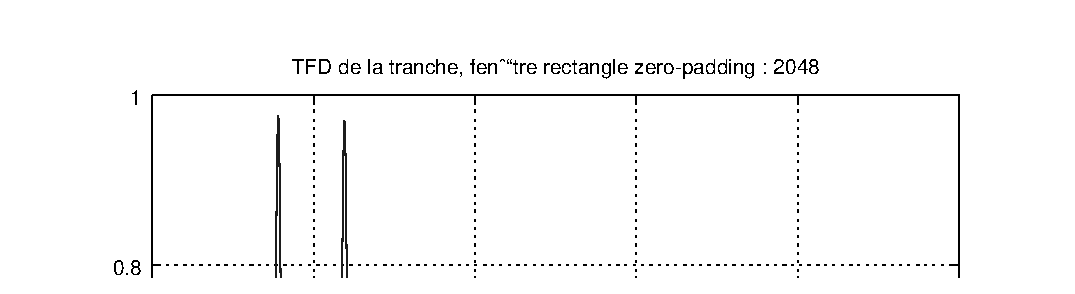
\includegraphics[width=\textwidth]{images/rectangle.eps}
  		% Title: glps_renderer figure
% Creator: GL2PS 1.3.8, (C) 1999-2012 C. Geuzaine
% For: Octave
% CreationDate: Wed Nov  8 10:42:42 2017
\begin{pgfpicture}
\pgfsetlinewidth{0.01pt}
\color[rgb]{1.000000,1.000000,1.000000}
\pgfpathmoveto{\pgfpoint{65.000015pt}{104.000000pt}}
\pgflineto{\pgfpoint{452.500031pt}{26.999981pt}}
\pgflineto{\pgfpoint{65.000015pt}{26.999981pt}}
\pgfpathclose
\pgfusepath{fill,stroke}
\pgfpathmoveto{\pgfpoint{65.000015pt}{104.000000pt}}
\pgflineto{\pgfpoint{452.500031pt}{104.000000pt}}
\pgflineto{\pgfpoint{452.500031pt}{26.999981pt}}
\pgfpathclose
\pgfusepath{fill,stroke}
\color[rgb]{0.000000,0.000000,0.000000}
\pgfsetlinewidth{0.500000pt}
\pgfsetdash{{16pt}{0pt}}{0pt}
\pgfpathmoveto{\pgfpoint{452.500031pt}{26.999981pt}}
\pgflineto{\pgfpoint{65.000015pt}{26.999981pt}}
\pgfusepath{stroke}
\pgfpathmoveto{\pgfpoint{452.500031pt}{104.000000pt}}
\pgflineto{\pgfpoint{65.000015pt}{104.000000pt}}
\pgfusepath{stroke}
\pgfpathmoveto{\pgfpoint{65.000015pt}{104.000000pt}}
\pgflineto{\pgfpoint{65.000015pt}{26.999981pt}}
\pgfusepath{stroke}
\pgfpathmoveto{\pgfpoint{452.500031pt}{104.000000pt}}
\pgflineto{\pgfpoint{452.500031pt}{26.999981pt}}
\pgfusepath{stroke}
\pgfsetdash{{0pt}{3pt}{1pt}{3pt}{1pt}{3pt}{1pt}{3pt}{1pt}{0pt}}{0pt}
\pgfpathmoveto{\pgfpoint{65.000015pt}{104.000000pt}}
\pgflineto{\pgfpoint{65.000015pt}{26.999981pt}}
\pgfusepath{stroke}
\pgfpathmoveto{\pgfpoint{142.500031pt}{104.000000pt}}
\pgflineto{\pgfpoint{142.500031pt}{26.999981pt}}
\pgfusepath{stroke}
\pgfpathmoveto{\pgfpoint{220.000031pt}{104.000000pt}}
\pgflineto{\pgfpoint{220.000031pt}{26.999981pt}}
\pgfusepath{stroke}
\pgfpathmoveto{\pgfpoint{297.500031pt}{104.000000pt}}
\pgflineto{\pgfpoint{297.500031pt}{26.999981pt}}
\pgfusepath{stroke}
\pgfpathmoveto{\pgfpoint{375.000061pt}{104.000000pt}}
\pgflineto{\pgfpoint{375.000061pt}{26.999981pt}}
\pgfusepath{stroke}
\pgfpathmoveto{\pgfpoint{452.500031pt}{104.000000pt}}
\pgflineto{\pgfpoint{452.500031pt}{26.999981pt}}
\pgfusepath{stroke}
\pgfsetdash{{16pt}{0pt}}{0pt}
\pgfpathmoveto{\pgfpoint{65.000015pt}{30.874983pt}}
\pgflineto{\pgfpoint{65.000015pt}{26.999981pt}}
\pgfusepath{stroke}
\pgfpathmoveto{\pgfpoint{65.000015pt}{100.125000pt}}
\pgflineto{\pgfpoint{65.000015pt}{104.000000pt}}
\pgfusepath{stroke}
\pgfpathmoveto{\pgfpoint{142.500031pt}{30.874983pt}}
\pgflineto{\pgfpoint{142.500031pt}{26.999981pt}}
\pgfusepath{stroke}
\pgfpathmoveto{\pgfpoint{142.500031pt}{100.125000pt}}
\pgflineto{\pgfpoint{142.500031pt}{104.000000pt}}
\pgfusepath{stroke}
\pgfpathmoveto{\pgfpoint{220.000031pt}{30.874983pt}}
\pgflineto{\pgfpoint{220.000031pt}{26.999981pt}}
\pgfusepath{stroke}
\pgfpathmoveto{\pgfpoint{220.000031pt}{100.125000pt}}
\pgflineto{\pgfpoint{220.000031pt}{104.000000pt}}
\pgfusepath{stroke}
\pgfpathmoveto{\pgfpoint{297.500031pt}{30.874983pt}}
\pgflineto{\pgfpoint{297.500031pt}{26.999981pt}}
\pgfusepath{stroke}
\pgfpathmoveto{\pgfpoint{297.500031pt}{100.125000pt}}
\pgflineto{\pgfpoint{297.500031pt}{104.000000pt}}
\pgfusepath{stroke}
\pgfpathmoveto{\pgfpoint{375.000061pt}{30.874983pt}}
\pgflineto{\pgfpoint{375.000061pt}{26.999981pt}}
\pgfusepath{stroke}
\pgfpathmoveto{\pgfpoint{375.000061pt}{100.125000pt}}
\pgflineto{\pgfpoint{375.000061pt}{104.000000pt}}
\pgfusepath{stroke}
\pgfpathmoveto{\pgfpoint{452.500031pt}{30.874983pt}}
\pgflineto{\pgfpoint{452.500031pt}{26.999981pt}}
\pgfusepath{stroke}
\pgfpathmoveto{\pgfpoint{452.500031pt}{100.125000pt}}
\pgflineto{\pgfpoint{452.500031pt}{104.000000pt}}
\pgfusepath{stroke}
{
\pgftransformshift{\pgfpoint{65.000015pt}{21.999977pt}}
\pgfnode{rectangle}{north}{\fontsize{10}{0}\selectfont\textcolor[rgb]{0,0,0}{{0}}}{}{\pgfusepath{discard}}}
{
\pgftransformshift{\pgfpoint{142.500015pt}{21.999977pt}}
\pgfnode{rectangle}{north}{\fontsize{10}{0}\selectfont\textcolor[rgb]{0,0,0}{{0.1}}}{}{\pgfusepath{discard}}}
{
\pgftransformshift{\pgfpoint{220.000015pt}{21.999977pt}}
\pgfnode{rectangle}{north}{\fontsize{10}{0}\selectfont\textcolor[rgb]{0,0,0}{{0.2}}}{}{\pgfusepath{discard}}}
{
\pgftransformshift{\pgfpoint{297.500031pt}{21.999977pt}}
\pgfnode{rectangle}{north}{\fontsize{10}{0}\selectfont\textcolor[rgb]{0,0,0}{{0.3}}}{}{\pgfusepath{discard}}}
{
\pgftransformshift{\pgfpoint{375.000031pt}{21.999977pt}}
\pgfnode{rectangle}{north}{\fontsize{10}{0}\selectfont\textcolor[rgb]{0,0,0}{{0.4}}}{}{\pgfusepath{discard}}}
{
\pgftransformshift{\pgfpoint{452.500031pt}{21.999977pt}}
\pgfnode{rectangle}{north}{\fontsize{10}{0}\selectfont\textcolor[rgb]{0,0,0}{{0.5}}}{}{\pgfusepath{discard}}}
\pgfsetdash{{0pt}{3pt}{1pt}{3pt}{1pt}{3pt}{1pt}{3pt}{1pt}{0pt}}{0pt}
\pgfpathmoveto{\pgfpoint{452.500031pt}{26.999981pt}}
\pgflineto{\pgfpoint{65.000015pt}{26.999981pt}}
\pgfusepath{stroke}
\pgfpathmoveto{\pgfpoint{452.500031pt}{42.399986pt}}
\pgflineto{\pgfpoint{65.000015pt}{42.399986pt}}
\pgfusepath{stroke}
\pgfpathmoveto{\pgfpoint{452.500031pt}{57.799988pt}}
\pgflineto{\pgfpoint{65.000015pt}{57.799988pt}}
\pgfusepath{stroke}
\pgfpathmoveto{\pgfpoint{452.500031pt}{73.199997pt}}
\pgflineto{\pgfpoint{65.000015pt}{73.199997pt}}
\pgfusepath{stroke}
\pgfpathmoveto{\pgfpoint{452.500031pt}{88.599998pt}}
\pgflineto{\pgfpoint{65.000015pt}{88.599998pt}}
\pgfusepath{stroke}
\pgfpathmoveto{\pgfpoint{452.500031pt}{104.000000pt}}
\pgflineto{\pgfpoint{65.000015pt}{104.000000pt}}
\pgfusepath{stroke}
\pgfsetdash{{16pt}{0pt}}{0pt}
\pgfpathmoveto{\pgfpoint{68.870026pt}{26.999981pt}}
\pgflineto{\pgfpoint{65.000015pt}{26.999981pt}}
\pgfusepath{stroke}
\pgfpathmoveto{\pgfpoint{448.630005pt}{26.999981pt}}
\pgflineto{\pgfpoint{452.500031pt}{26.999981pt}}
\pgfusepath{stroke}
\pgfpathmoveto{\pgfpoint{68.870026pt}{42.399986pt}}
\pgflineto{\pgfpoint{65.000015pt}{42.399986pt}}
\pgfusepath{stroke}
\pgfpathmoveto{\pgfpoint{448.630005pt}{42.399986pt}}
\pgflineto{\pgfpoint{452.500031pt}{42.399986pt}}
\pgfusepath{stroke}
\pgfpathmoveto{\pgfpoint{68.870026pt}{57.799988pt}}
\pgflineto{\pgfpoint{65.000015pt}{57.799988pt}}
\pgfusepath{stroke}
\pgfpathmoveto{\pgfpoint{448.630005pt}{57.799988pt}}
\pgflineto{\pgfpoint{452.500031pt}{57.799988pt}}
\pgfusepath{stroke}
\pgfpathmoveto{\pgfpoint{68.870026pt}{73.199997pt}}
\pgflineto{\pgfpoint{65.000015pt}{73.199997pt}}
\pgfusepath{stroke}
\pgfpathmoveto{\pgfpoint{448.630005pt}{73.199997pt}}
\pgflineto{\pgfpoint{452.500031pt}{73.199997pt}}
\pgfusepath{stroke}
\pgfpathmoveto{\pgfpoint{68.870026pt}{88.599998pt}}
\pgflineto{\pgfpoint{65.000015pt}{88.599998pt}}
\pgfusepath{stroke}
\pgfpathmoveto{\pgfpoint{448.630005pt}{88.599998pt}}
\pgflineto{\pgfpoint{452.500031pt}{88.599998pt}}
\pgfusepath{stroke}
\pgfpathmoveto{\pgfpoint{68.870026pt}{104.000000pt}}
\pgflineto{\pgfpoint{65.000015pt}{104.000000pt}}
\pgfusepath{stroke}
\pgfpathmoveto{\pgfpoint{448.630005pt}{104.000000pt}}
\pgflineto{\pgfpoint{452.500031pt}{104.000000pt}}
\pgfusepath{stroke}
{
\pgftransformshift{\pgfpoint{60.006454pt}{26.999981pt}}
\pgfnode{rectangle}{east}{\fontsize{10}{0}\selectfont\textcolor[rgb]{0,0,0}{{0}}}{}{\pgfusepath{discard}}}
{
\pgftransformshift{\pgfpoint{60.006454pt}{42.399986pt}}
\pgfnode{rectangle}{east}{\fontsize{10}{0}\selectfont\textcolor[rgb]{0,0,0}{{0.2}}}{}{\pgfusepath{discard}}}
{
\pgftransformshift{\pgfpoint{60.006454pt}{57.799988pt}}
\pgfnode{rectangle}{east}{\fontsize{10}{0}\selectfont\textcolor[rgb]{0,0,0}{{0.4}}}{}{\pgfusepath{discard}}}
{
\pgftransformshift{\pgfpoint{60.006454pt}{73.199997pt}}
\pgfnode{rectangle}{east}{\fontsize{10}{0}\selectfont\textcolor[rgb]{0,0,0}{{0.6}}}{}{\pgfusepath{discard}}}
{
\pgftransformshift{\pgfpoint{60.006454pt}{88.599998pt}}
\pgfnode{rectangle}{east}{\fontsize{10}{0}\selectfont\textcolor[rgb]{0,0,0}{{0.8}}}{}{\pgfusepath{discard}}}
{
\pgftransformshift{\pgfpoint{60.006454pt}{104.000000pt}}
\pgfnode{rectangle}{east}{\fontsize{10}{0}\selectfont\textcolor[rgb]{0,0,0}{{1}}}{}{\pgfusepath{discard}}}
{
\pgftransformshift{\pgfpoint{258.750031pt}{10.999977pt}}
\pgfnode{rectangle}{north}{\fontsize{10}{0}\selectfont\textcolor[rgb]{0,0,0}{{Fréquence (Hz)}}}{}{\pgfusepath{discard}}}
\color[rgb]{0.000000,0.000000,1.000000}
\pgfsetdash{}{0pt}
\pgfpathmoveto{\pgfpoint{65.189224pt}{27.895466pt}}
\pgflineto{\pgfpoint{65.000015pt}{27.905190pt}}
\pgfusepath{stroke}
\pgfpathmoveto{\pgfpoint{65.378433pt}{27.866982pt}}
\pgflineto{\pgfpoint{65.189224pt}{27.895466pt}}
\pgfusepath{stroke}
\pgfpathmoveto{\pgfpoint{65.567642pt}{27.821846pt}}
\pgflineto{\pgfpoint{65.378433pt}{27.866982pt}}
\pgfusepath{stroke}
\pgfpathmoveto{\pgfpoint{65.756836pt}{27.763756pt}}
\pgflineto{\pgfpoint{65.567642pt}{27.821846pt}}
\pgfusepath{stroke}
\pgfpathmoveto{\pgfpoint{65.946060pt}{27.698292pt}}
\pgflineto{\pgfpoint{65.756836pt}{27.763756pt}}
\pgfusepath{stroke}
\pgfpathmoveto{\pgfpoint{66.135269pt}{27.633350pt}}
\pgflineto{\pgfpoint{65.946060pt}{27.698292pt}}
\pgfusepath{stroke}
\pgfpathmoveto{\pgfpoint{66.324478pt}{27.579254pt}}
\pgflineto{\pgfpoint{66.135269pt}{27.633350pt}}
\pgfusepath{stroke}
\pgfpathmoveto{\pgfpoint{66.513687pt}{27.547531pt}}
\pgflineto{\pgfpoint{66.324478pt}{27.579254pt}}
\pgfusepath{stroke}
\pgfpathmoveto{\pgfpoint{66.702881pt}{27.546761pt}}
\pgflineto{\pgfpoint{66.513687pt}{27.547531pt}}
\pgfusepath{stroke}
\pgfpathmoveto{\pgfpoint{66.892105pt}{27.577461pt}}
\pgflineto{\pgfpoint{66.702881pt}{27.546761pt}}
\pgfusepath{stroke}
\pgfpathmoveto{\pgfpoint{67.081314pt}{27.631725pt}}
\pgflineto{\pgfpoint{66.892105pt}{27.577461pt}}
\pgfusepath{stroke}
\pgfpathmoveto{\pgfpoint{67.270523pt}{27.698112pt}}
\pgflineto{\pgfpoint{67.081314pt}{27.631725pt}}
\pgfusepath{stroke}
\pgfpathmoveto{\pgfpoint{67.459732pt}{27.765999pt}}
\pgflineto{\pgfpoint{67.270523pt}{27.698112pt}}
\pgfusepath{stroke}
\pgfpathmoveto{\pgfpoint{67.648926pt}{27.827122pt}}
\pgflineto{\pgfpoint{67.459732pt}{27.765999pt}}
\pgfusepath{stroke}
\pgfpathmoveto{\pgfpoint{67.838150pt}{27.875477pt}}
\pgflineto{\pgfpoint{67.648926pt}{27.827122pt}}
\pgfusepath{stroke}
\pgfpathmoveto{\pgfpoint{68.027359pt}{27.906971pt}}
\pgflineto{\pgfpoint{67.838150pt}{27.875477pt}}
\pgfusepath{stroke}
\pgfpathmoveto{\pgfpoint{68.216568pt}{27.919109pt}}
\pgflineto{\pgfpoint{68.027359pt}{27.906971pt}}
\pgfusepath{stroke}
\pgfpathmoveto{\pgfpoint{68.405777pt}{27.910881pt}}
\pgflineto{\pgfpoint{68.216568pt}{27.919109pt}}
\pgfusepath{stroke}
\pgfpathmoveto{\pgfpoint{68.594971pt}{27.882668pt}}
\pgflineto{\pgfpoint{68.405777pt}{27.910881pt}}
\pgfusepath{stroke}
\pgfpathmoveto{\pgfpoint{68.784195pt}{27.836376pt}}
\pgflineto{\pgfpoint{68.594971pt}{27.882668pt}}
\pgfusepath{stroke}
\pgfpathmoveto{\pgfpoint{68.973404pt}{27.775593pt}}
\pgflineto{\pgfpoint{68.784195pt}{27.836376pt}}
\pgfusepath{stroke}
\pgfpathmoveto{\pgfpoint{69.162613pt}{27.705997pt}}
\pgflineto{\pgfpoint{68.973404pt}{27.775593pt}}
\pgfusepath{stroke}
\pgfpathmoveto{\pgfpoint{69.351822pt}{27.635921pt}}
\pgflineto{\pgfpoint{69.162613pt}{27.705997pt}}
\pgfusepath{stroke}
\pgfpathmoveto{\pgfpoint{69.541016pt}{27.576790pt}}
\pgflineto{\pgfpoint{69.351822pt}{27.635921pt}}
\pgfusepath{stroke}
\pgfpathmoveto{\pgfpoint{69.730240pt}{27.541985pt}}
\pgflineto{\pgfpoint{69.541016pt}{27.576790pt}}
\pgfusepath{stroke}
\pgfpathmoveto{\pgfpoint{69.919449pt}{27.542011pt}}
\pgflineto{\pgfpoint{69.730240pt}{27.541985pt}}
\pgfusepath{stroke}
\pgfpathmoveto{\pgfpoint{70.108658pt}{27.577724pt}}
\pgflineto{\pgfpoint{69.919449pt}{27.542011pt}}
\pgfusepath{stroke}
\pgfpathmoveto{\pgfpoint{70.297867pt}{27.639744pt}}
\pgflineto{\pgfpoint{70.108658pt}{27.577724pt}}
\pgfusepath{stroke}
\pgfpathmoveto{\pgfpoint{70.487061pt}{27.714764pt}}
\pgflineto{\pgfpoint{70.297867pt}{27.639744pt}}
\pgfusepath{stroke}
\pgfpathmoveto{\pgfpoint{70.676285pt}{27.790840pt}}
\pgflineto{\pgfpoint{70.487061pt}{27.714764pt}}
\pgfusepath{stroke}
\pgfpathmoveto{\pgfpoint{70.865494pt}{27.858871pt}}
\pgflineto{\pgfpoint{70.676285pt}{27.790840pt}}
\pgfusepath{stroke}
\pgfpathmoveto{\pgfpoint{71.054703pt}{27.912331pt}}
\pgflineto{\pgfpoint{70.865494pt}{27.858871pt}}
\pgfusepath{stroke}
\pgfpathmoveto{\pgfpoint{71.243912pt}{27.946739pt}}
\pgflineto{\pgfpoint{71.054703pt}{27.912331pt}}
\pgfusepath{stroke}
\pgfpathmoveto{\pgfpoint{71.433105pt}{27.959373pt}}
\pgflineto{\pgfpoint{71.243912pt}{27.946739pt}}
\pgfusepath{stroke}
\pgfpathmoveto{\pgfpoint{71.622330pt}{27.949062pt}}
\pgflineto{\pgfpoint{71.433105pt}{27.959373pt}}
\pgfusepath{stroke}
\pgfpathmoveto{\pgfpoint{71.811539pt}{27.916191pt}}
\pgflineto{\pgfpoint{71.622330pt}{27.949062pt}}
\pgfusepath{stroke}
\pgfpathmoveto{\pgfpoint{72.000748pt}{27.862808pt}}
\pgflineto{\pgfpoint{71.811539pt}{27.916191pt}}
\pgfusepath{stroke}
\pgfpathmoveto{\pgfpoint{72.189957pt}{27.792912pt}}
\pgflineto{\pgfpoint{72.000748pt}{27.862808pt}}
\pgfusepath{stroke}
\pgfpathmoveto{\pgfpoint{72.379150pt}{27.712959pt}}
\pgflineto{\pgfpoint{72.189957pt}{27.792912pt}}
\pgfusepath{stroke}
\pgfpathmoveto{\pgfpoint{72.568375pt}{27.632786pt}}
\pgflineto{\pgfpoint{72.379150pt}{27.712959pt}}
\pgfusepath{stroke}
\pgfpathmoveto{\pgfpoint{72.757584pt}{27.566479pt}}
\pgflineto{\pgfpoint{72.568375pt}{27.632786pt}}
\pgfusepath{stroke}
\pgfpathmoveto{\pgfpoint{72.946793pt}{27.531090pt}}
\pgflineto{\pgfpoint{72.757584pt}{27.566479pt}}
\pgfusepath{stroke}
\pgfpathmoveto{\pgfpoint{73.136002pt}{27.539291pt}}
\pgflineto{\pgfpoint{72.946793pt}{27.531090pt}}
\pgfusepath{stroke}
\pgfpathmoveto{\pgfpoint{73.325195pt}{27.589619pt}}
\pgflineto{\pgfpoint{73.136002pt}{27.539291pt}}
\pgfusepath{stroke}
\pgfpathmoveto{\pgfpoint{73.514420pt}{27.667992pt}}
\pgflineto{\pgfpoint{73.325195pt}{27.589619pt}}
\pgfusepath{stroke}
\pgfpathmoveto{\pgfpoint{73.703629pt}{27.757740pt}}
\pgflineto{\pgfpoint{73.514420pt}{27.667992pt}}
\pgfusepath{stroke}
\pgfpathmoveto{\pgfpoint{73.892838pt}{27.845417pt}}
\pgflineto{\pgfpoint{73.703629pt}{27.757740pt}}
\pgfusepath{stroke}
\pgfpathmoveto{\pgfpoint{74.082047pt}{27.921337pt}}
\pgflineto{\pgfpoint{73.892838pt}{27.845417pt}}
\pgfusepath{stroke}
\pgfpathmoveto{\pgfpoint{74.271240pt}{27.978748pt}}
\pgflineto{\pgfpoint{74.082047pt}{27.921337pt}}
\pgfusepath{stroke}
\pgfpathmoveto{\pgfpoint{74.460464pt}{28.013134pt}}
\pgflineto{\pgfpoint{74.271240pt}{27.978748pt}}
\pgfusepath{stroke}
\pgfpathmoveto{\pgfpoint{74.649673pt}{28.021816pt}}
\pgflineto{\pgfpoint{74.460464pt}{28.013134pt}}
\pgfusepath{stroke}
\pgfpathmoveto{\pgfpoint{74.838882pt}{28.003849pt}}
\pgflineto{\pgfpoint{74.649673pt}{28.021816pt}}
\pgfusepath{stroke}
\pgfpathmoveto{\pgfpoint{75.028091pt}{27.959995pt}}
\pgflineto{\pgfpoint{74.838882pt}{28.003849pt}}
\pgfusepath{stroke}
\pgfpathmoveto{\pgfpoint{75.217285pt}{27.892921pt}}
\pgflineto{\pgfpoint{75.028091pt}{27.959995pt}}
\pgfusepath{stroke}
\pgfpathmoveto{\pgfpoint{75.406509pt}{27.807590pt}}
\pgflineto{\pgfpoint{75.217285pt}{27.892921pt}}
\pgfusepath{stroke}
\pgfpathmoveto{\pgfpoint{75.595718pt}{27.712097pt}}
\pgflineto{\pgfpoint{75.406509pt}{27.807590pt}}
\pgfusepath{stroke}
\pgfpathmoveto{\pgfpoint{75.784927pt}{27.619160pt}}
\pgflineto{\pgfpoint{75.595718pt}{27.712097pt}}
\pgfusepath{stroke}
\pgfpathmoveto{\pgfpoint{75.974136pt}{27.547726pt}}
\pgflineto{\pgfpoint{75.784927pt}{27.619160pt}}
\pgfusepath{stroke}
\pgfpathmoveto{\pgfpoint{76.163330pt}{27.520344pt}}
\pgflineto{\pgfpoint{75.974136pt}{27.547726pt}}
\pgfusepath{stroke}
\pgfpathmoveto{\pgfpoint{76.352554pt}{27.549557pt}}
\pgflineto{\pgfpoint{76.163330pt}{27.520344pt}}
\pgfusepath{stroke}
\pgfpathmoveto{\pgfpoint{76.541763pt}{27.625851pt}}
\pgflineto{\pgfpoint{76.352554pt}{27.549557pt}}
\pgfusepath{stroke}
\pgfpathmoveto{\pgfpoint{76.730972pt}{27.727509pt}}
\pgflineto{\pgfpoint{76.541763pt}{27.625851pt}}
\pgfusepath{stroke}
\pgfpathmoveto{\pgfpoint{76.920181pt}{27.834904pt}}
\pgflineto{\pgfpoint{76.730972pt}{27.727509pt}}
\pgfusepath{stroke}
\pgfpathmoveto{\pgfpoint{77.109375pt}{27.934105pt}}
\pgflineto{\pgfpoint{76.920181pt}{27.834904pt}}
\pgfusepath{stroke}
\pgfpathmoveto{\pgfpoint{77.298599pt}{28.015614pt}}
\pgflineto{\pgfpoint{77.109375pt}{27.934105pt}}
\pgfusepath{stroke}
\pgfpathmoveto{\pgfpoint{77.487808pt}{28.072968pt}}
\pgflineto{\pgfpoint{77.298599pt}{28.015614pt}}
\pgfusepath{stroke}
\pgfpathmoveto{\pgfpoint{77.677017pt}{28.101986pt}}
\pgflineto{\pgfpoint{77.487808pt}{28.072968pt}}
\pgfusepath{stroke}
\pgfpathmoveto{\pgfpoint{77.866226pt}{28.100422pt}}
\pgflineto{\pgfpoint{77.677017pt}{28.101986pt}}
\pgfusepath{stroke}
\pgfpathmoveto{\pgfpoint{78.055420pt}{28.067917pt}}
\pgflineto{\pgfpoint{77.866226pt}{28.100422pt}}
\pgfusepath{stroke}
\pgfpathmoveto{\pgfpoint{78.244644pt}{28.006020pt}}
\pgflineto{\pgfpoint{78.055420pt}{28.067917pt}}
\pgfusepath{stroke}
\pgfpathmoveto{\pgfpoint{78.433853pt}{27.918522pt}}
\pgflineto{\pgfpoint{78.244644pt}{28.006020pt}}
\pgfusepath{stroke}
\pgfpathmoveto{\pgfpoint{78.623062pt}{27.812057pt}}
\pgflineto{\pgfpoint{78.433853pt}{27.918522pt}}
\pgfusepath{stroke}
\pgfpathmoveto{\pgfpoint{78.812271pt}{27.697517pt}}
\pgflineto{\pgfpoint{78.623062pt}{27.812057pt}}
\pgfusepath{stroke}
\pgfpathmoveto{\pgfpoint{79.001465pt}{27.592743pt}}
\pgflineto{\pgfpoint{78.812271pt}{27.697517pt}}
\pgfusepath{stroke}
\pgfpathmoveto{\pgfpoint{79.190689pt}{27.524937pt}}
\pgflineto{\pgfpoint{79.001465pt}{27.592743pt}}
\pgfusepath{stroke}
\pgfpathmoveto{\pgfpoint{79.379898pt}{27.522373pt}}
\pgflineto{\pgfpoint{79.190689pt}{27.524937pt}}
\pgfusepath{stroke}
\pgfpathmoveto{\pgfpoint{79.569107pt}{27.588898pt}}
\pgflineto{\pgfpoint{79.379898pt}{27.522373pt}}
\pgfusepath{stroke}
\pgfpathmoveto{\pgfpoint{79.758316pt}{27.699867pt}}
\pgflineto{\pgfpoint{79.569107pt}{27.588898pt}}
\pgfusepath{stroke}
\pgfpathmoveto{\pgfpoint{79.947510pt}{27.827126pt}}
\pgflineto{\pgfpoint{79.758316pt}{27.699867pt}}
\pgfusepath{stroke}
\pgfpathmoveto{\pgfpoint{80.136734pt}{27.950798pt}}
\pgflineto{\pgfpoint{79.947510pt}{27.827126pt}}
\pgfusepath{stroke}
\pgfpathmoveto{\pgfpoint{80.325943pt}{28.057938pt}}
\pgflineto{\pgfpoint{80.136734pt}{27.950798pt}}
\pgfusepath{stroke}
\pgfpathmoveto{\pgfpoint{80.515152pt}{28.139896pt}}
\pgflineto{\pgfpoint{80.325943pt}{28.057938pt}}
\pgfusepath{stroke}
\pgfpathmoveto{\pgfpoint{80.704361pt}{28.190899pt}}
\pgflineto{\pgfpoint{80.515152pt}{28.139896pt}}
\pgfusepath{stroke}
\pgfpathmoveto{\pgfpoint{80.893570pt}{28.207432pt}}
\pgflineto{\pgfpoint{80.704361pt}{28.190899pt}}
\pgfusepath{stroke}
\pgfpathmoveto{\pgfpoint{81.082779pt}{28.188019pt}}
\pgflineto{\pgfpoint{80.893570pt}{28.207432pt}}
\pgfusepath{stroke}
\pgfpathmoveto{\pgfpoint{81.271988pt}{28.133247pt}}
\pgflineto{\pgfpoint{81.082779pt}{28.188019pt}}
\pgfusepath{stroke}
\pgfpathmoveto{\pgfpoint{81.461197pt}{28.045914pt}}
\pgflineto{\pgfpoint{81.271988pt}{28.133247pt}}
\pgfusepath{stroke}
\pgfpathmoveto{\pgfpoint{81.650406pt}{27.931522pt}}
\pgflineto{\pgfpoint{81.461197pt}{28.045914pt}}
\pgfusepath{stroke}
\pgfpathmoveto{\pgfpoint{81.839615pt}{27.799370pt}}
\pgflineto{\pgfpoint{81.650406pt}{27.931522pt}}
\pgfusepath{stroke}
\pgfpathmoveto{\pgfpoint{82.028824pt}{27.665180pt}}
\pgflineto{\pgfpoint{81.839615pt}{27.799370pt}}
\pgfusepath{stroke}
\pgfpathmoveto{\pgfpoint{82.218033pt}{27.556076pt}}
\pgflineto{\pgfpoint{82.028824pt}{27.665180pt}}
\pgfusepath{stroke}
\pgfpathmoveto{\pgfpoint{82.407242pt}{27.511875pt}}
\pgflineto{\pgfpoint{82.218033pt}{27.556076pt}}
\pgfusepath{stroke}
\pgfpathmoveto{\pgfpoint{82.596451pt}{27.558273pt}}
\pgflineto{\pgfpoint{82.407242pt}{27.511875pt}}
\pgfusepath{stroke}
\pgfpathmoveto{\pgfpoint{82.785660pt}{27.674633pt}}
\pgflineto{\pgfpoint{82.596451pt}{27.558273pt}}
\pgfusepath{stroke}
\pgfpathmoveto{\pgfpoint{82.974869pt}{27.821884pt}}
\pgflineto{\pgfpoint{82.785660pt}{27.674633pt}}
\pgfusepath{stroke}
\pgfpathmoveto{\pgfpoint{83.164078pt}{27.971638pt}}
\pgflineto{\pgfpoint{82.974869pt}{27.821884pt}}
\pgfusepath{stroke}
\pgfpathmoveto{\pgfpoint{83.353287pt}{28.106464pt}}
\pgflineto{\pgfpoint{83.164078pt}{27.971638pt}}
\pgfusepath{stroke}
\pgfpathmoveto{\pgfpoint{83.542496pt}{28.215183pt}}
\pgflineto{\pgfpoint{83.353287pt}{28.106464pt}}
\pgfusepath{stroke}
\pgfpathmoveto{\pgfpoint{83.731705pt}{28.290287pt}}
\pgflineto{\pgfpoint{83.542496pt}{28.215183pt}}
\pgfusepath{stroke}
\pgfpathmoveto{\pgfpoint{83.920914pt}{28.326912pt}}
\pgflineto{\pgfpoint{83.731705pt}{28.290287pt}}
\pgfusepath{stroke}
\pgfpathmoveto{\pgfpoint{84.110123pt}{28.322487pt}}
\pgflineto{\pgfpoint{83.920914pt}{28.326912pt}}
\pgfusepath{stroke}
\pgfpathmoveto{\pgfpoint{84.299332pt}{28.276638pt}}
\pgflineto{\pgfpoint{84.110123pt}{28.322487pt}}
\pgfusepath{stroke}
\pgfpathmoveto{\pgfpoint{84.488541pt}{28.191303pt}}
\pgflineto{\pgfpoint{84.299332pt}{28.276638pt}}
\pgfusepath{stroke}
\pgfpathmoveto{\pgfpoint{84.677750pt}{28.071072pt}}
\pgflineto{\pgfpoint{84.488541pt}{28.191303pt}}
\pgfusepath{stroke}
\pgfpathmoveto{\pgfpoint{84.866959pt}{27.924007pt}}
\pgflineto{\pgfpoint{84.677750pt}{28.071072pt}}
\pgfusepath{stroke}
\pgfpathmoveto{\pgfpoint{85.056168pt}{27.763813pt}}
\pgflineto{\pgfpoint{84.866959pt}{27.924007pt}}
\pgfusepath{stroke}
\pgfpathmoveto{\pgfpoint{85.245377pt}{27.615173pt}}
\pgflineto{\pgfpoint{85.056168pt}{27.763813pt}}
\pgfusepath{stroke}
\pgfpathmoveto{\pgfpoint{85.434586pt}{27.522411pt}}
\pgflineto{\pgfpoint{85.245377pt}{27.615173pt}}
\pgfusepath{stroke}
\pgfpathmoveto{\pgfpoint{85.623795pt}{27.535946pt}}
\pgflineto{\pgfpoint{85.434586pt}{27.522411pt}}
\pgfusepath{stroke}
\pgfpathmoveto{\pgfpoint{85.813004pt}{27.651722pt}}
\pgflineto{\pgfpoint{85.623795pt}{27.535946pt}}
\pgfusepath{stroke}
\pgfpathmoveto{\pgfpoint{86.002213pt}{27.818943pt}}
\pgflineto{\pgfpoint{85.813004pt}{27.651722pt}}
\pgfusepath{stroke}
\pgfpathmoveto{\pgfpoint{86.191422pt}{27.996906pt}}
\pgflineto{\pgfpoint{86.002213pt}{27.818943pt}}
\pgfusepath{stroke}
\pgfpathmoveto{\pgfpoint{86.380630pt}{28.162159pt}}
\pgflineto{\pgfpoint{86.191422pt}{27.996906pt}}
\pgfusepath{stroke}
\pgfpathmoveto{\pgfpoint{86.569839pt}{28.300465pt}}
\pgflineto{\pgfpoint{86.380630pt}{28.162159pt}}
\pgfusepath{stroke}
\pgfpathmoveto{\pgfpoint{86.759048pt}{28.402386pt}}
\pgflineto{\pgfpoint{86.569839pt}{28.300465pt}}
\pgfusepath{stroke}
\pgfpathmoveto{\pgfpoint{86.948257pt}{28.461605pt}}
\pgflineto{\pgfpoint{86.759048pt}{28.402386pt}}
\pgfusepath{stroke}
\pgfpathmoveto{\pgfpoint{87.137466pt}{28.474369pt}}
\pgflineto{\pgfpoint{86.948257pt}{28.461605pt}}
\pgfusepath{stroke}
\pgfpathmoveto{\pgfpoint{87.326675pt}{28.439327pt}}
\pgflineto{\pgfpoint{87.137466pt}{28.474369pt}}
\pgfusepath{stroke}
\pgfpathmoveto{\pgfpoint{87.515884pt}{28.357597pt}}
\pgflineto{\pgfpoint{87.326675pt}{28.439327pt}}
\pgfusepath{stroke}
\pgfpathmoveto{\pgfpoint{87.705093pt}{28.232990pt}}
\pgflineto{\pgfpoint{87.515884pt}{28.357597pt}}
\pgfusepath{stroke}
\pgfpathmoveto{\pgfpoint{87.894302pt}{28.072636pt}}
\pgflineto{\pgfpoint{87.705093pt}{28.232990pt}}
\pgfusepath{stroke}
\pgfpathmoveto{\pgfpoint{88.083511pt}{27.888649pt}}
\pgflineto{\pgfpoint{87.894302pt}{28.072636pt}}
\pgfusepath{stroke}
\pgfpathmoveto{\pgfpoint{88.272720pt}{27.702793pt}}
\pgflineto{\pgfpoint{88.083511pt}{27.888649pt}}
\pgfusepath{stroke}
\pgfpathmoveto{\pgfpoint{88.461929pt}{27.558174pt}}
\pgflineto{\pgfpoint{88.272720pt}{27.702793pt}}
\pgfusepath{stroke}
\pgfpathmoveto{\pgfpoint{88.651138pt}{27.525002pt}}
\pgflineto{\pgfpoint{88.461929pt}{27.558174pt}}
\pgfusepath{stroke}
\pgfpathmoveto{\pgfpoint{88.840347pt}{27.631226pt}}
\pgflineto{\pgfpoint{88.651138pt}{27.525002pt}}
\pgfusepath{stroke}
\pgfpathmoveto{\pgfpoint{89.029556pt}{27.818027pt}}
\pgflineto{\pgfpoint{88.840347pt}{27.631226pt}}
\pgfusepath{stroke}
\pgfpathmoveto{\pgfpoint{89.218765pt}{28.026962pt}}
\pgflineto{\pgfpoint{89.029556pt}{27.818027pt}}
\pgfusepath{stroke}
\pgfpathmoveto{\pgfpoint{89.407974pt}{28.226246pt}}
\pgflineto{\pgfpoint{89.218765pt}{28.026962pt}}
\pgfusepath{stroke}
\pgfpathmoveto{\pgfpoint{89.597183pt}{28.397861pt}}
\pgflineto{\pgfpoint{89.407974pt}{28.226246pt}}
\pgfusepath{stroke}
\pgfpathmoveto{\pgfpoint{89.786392pt}{28.530151pt}}
\pgflineto{\pgfpoint{89.597183pt}{28.397861pt}}
\pgfusepath{stroke}
\pgfpathmoveto{\pgfpoint{89.975601pt}{28.615170pt}}
\pgflineto{\pgfpoint{89.786392pt}{28.530151pt}}
\pgfusepath{stroke}
\pgfpathmoveto{\pgfpoint{90.164810pt}{28.647865pt}}
\pgflineto{\pgfpoint{89.975601pt}{28.615170pt}}
\pgfusepath{stroke}
\pgfpathmoveto{\pgfpoint{90.354019pt}{28.625839pt}}
\pgflineto{\pgfpoint{90.164810pt}{28.647865pt}}
\pgfusepath{stroke}
\pgfpathmoveto{\pgfpoint{90.543228pt}{28.549339pt}}
\pgflineto{\pgfpoint{90.354019pt}{28.625839pt}}
\pgfusepath{stroke}
\pgfpathmoveto{\pgfpoint{90.732437pt}{28.421471pt}}
\pgflineto{\pgfpoint{90.543228pt}{28.549339pt}}
\pgfusepath{stroke}
\pgfpathmoveto{\pgfpoint{90.921646pt}{28.248631pt}}
\pgflineto{\pgfpoint{90.732437pt}{28.421471pt}}
\pgfusepath{stroke}
\pgfpathmoveto{\pgfpoint{91.110855pt}{28.041771pt}}
\pgflineto{\pgfpoint{90.921646pt}{28.248631pt}}
\pgfusepath{stroke}
\pgfpathmoveto{\pgfpoint{91.300064pt}{27.820152pt}}
\pgflineto{\pgfpoint{91.110855pt}{28.041771pt}}
\pgfusepath{stroke}
\pgfpathmoveto{\pgfpoint{91.489273pt}{27.622807pt}}
\pgflineto{\pgfpoint{91.300064pt}{27.820152pt}}
\pgfusepath{stroke}
\pgfpathmoveto{\pgfpoint{91.678482pt}{27.529949pt}}
\pgflineto{\pgfpoint{91.489273pt}{27.622807pt}}
\pgfusepath{stroke}
\pgfpathmoveto{\pgfpoint{91.867691pt}{27.613575pt}}
\pgflineto{\pgfpoint{91.678482pt}{27.529949pt}}
\pgfusepath{stroke}
\pgfpathmoveto{\pgfpoint{92.056900pt}{27.818760pt}}
\pgflineto{\pgfpoint{91.867691pt}{27.613575pt}}
\pgfusepath{stroke}
\pgfpathmoveto{\pgfpoint{92.246109pt}{28.062263pt}}
\pgflineto{\pgfpoint{92.056900pt}{27.818760pt}}
\pgfusepath{stroke}
\pgfpathmoveto{\pgfpoint{92.435318pt}{28.300354pt}}
\pgflineto{\pgfpoint{92.246109pt}{28.062263pt}}
\pgfusepath{stroke}
\pgfpathmoveto{\pgfpoint{92.624527pt}{28.510216pt}}
\pgflineto{\pgfpoint{92.435318pt}{28.300354pt}}
\pgfusepath{stroke}
\pgfpathmoveto{\pgfpoint{92.813736pt}{28.677570pt}}
\pgflineto{\pgfpoint{92.624527pt}{28.510216pt}}
\pgfusepath{stroke}
\pgfpathmoveto{\pgfpoint{93.002945pt}{28.792618pt}}
\pgflineto{\pgfpoint{92.813736pt}{28.677570pt}}
\pgfusepath{stroke}
\pgfpathmoveto{\pgfpoint{93.192154pt}{28.848816pt}}
\pgflineto{\pgfpoint{93.002945pt}{28.792618pt}}
\pgfusepath{stroke}
\pgfpathmoveto{\pgfpoint{93.381363pt}{28.842567pt}}
\pgflineto{\pgfpoint{93.192154pt}{28.848816pt}}
\pgfusepath{stroke}
\pgfpathmoveto{\pgfpoint{93.570572pt}{28.773190pt}}
\pgflineto{\pgfpoint{93.381363pt}{28.842567pt}}
\pgfusepath{stroke}
\pgfpathmoveto{\pgfpoint{93.759781pt}{28.643051pt}}
\pgflineto{\pgfpoint{93.570572pt}{28.773190pt}}
\pgfusepath{stroke}
\pgfpathmoveto{\pgfpoint{93.948990pt}{28.457935pt}}
\pgflineto{\pgfpoint{93.759781pt}{28.643051pt}}
\pgfusepath{stroke}
\pgfpathmoveto{\pgfpoint{94.138199pt}{28.227966pt}}
\pgflineto{\pgfpoint{93.948990pt}{28.457935pt}}
\pgfusepath{stroke}
\pgfpathmoveto{\pgfpoint{94.327408pt}{27.970520pt}}
\pgflineto{\pgfpoint{94.138199pt}{28.227966pt}}
\pgfusepath{stroke}
\pgfpathmoveto{\pgfpoint{94.516617pt}{27.720020pt}}
\pgflineto{\pgfpoint{94.327408pt}{27.970520pt}}
\pgfusepath{stroke}
\pgfpathmoveto{\pgfpoint{94.705826pt}{27.556854pt}}
\pgflineto{\pgfpoint{94.516617pt}{27.720020pt}}
\pgfusepath{stroke}
\pgfpathmoveto{\pgfpoint{94.895035pt}{27.599838pt}}
\pgflineto{\pgfpoint{94.705826pt}{27.556854pt}}
\pgfusepath{stroke}
\pgfpathmoveto{\pgfpoint{95.084244pt}{27.820606pt}}
\pgflineto{\pgfpoint{94.895035pt}{27.599838pt}}
\pgfusepath{stroke}
\pgfpathmoveto{\pgfpoint{95.273453pt}{28.103363pt}}
\pgflineto{\pgfpoint{95.084244pt}{27.820606pt}}
\pgfusepath{stroke}
\pgfpathmoveto{\pgfpoint{95.462662pt}{28.386673pt}}
\pgflineto{\pgfpoint{95.273453pt}{28.103363pt}}
\pgfusepath{stroke}
\pgfpathmoveto{\pgfpoint{95.651871pt}{28.641426pt}}
\pgflineto{\pgfpoint{95.462662pt}{28.386673pt}}
\pgfusepath{stroke}
\pgfpathmoveto{\pgfpoint{95.841080pt}{28.850178pt}}
\pgflineto{\pgfpoint{95.651871pt}{28.641426pt}}
\pgfusepath{stroke}
\pgfpathmoveto{\pgfpoint{96.030289pt}{29.000946pt}}
\pgflineto{\pgfpoint{95.841080pt}{28.850178pt}}
\pgfusepath{stroke}
\pgfpathmoveto{\pgfpoint{96.219498pt}{29.085445pt}}
\pgflineto{\pgfpoint{96.030289pt}{29.000946pt}}
\pgfusepath{stroke}
\pgfpathmoveto{\pgfpoint{96.408707pt}{29.098682pt}}
\pgflineto{\pgfpoint{96.219498pt}{29.085445pt}}
\pgfusepath{stroke}
\pgfpathmoveto{\pgfpoint{96.597916pt}{29.038864pt}}
\pgflineto{\pgfpoint{96.408707pt}{29.098682pt}}
\pgfusepath{stroke}
\pgfpathmoveto{\pgfpoint{96.787125pt}{28.907555pt}}
\pgflineto{\pgfpoint{96.597916pt}{29.038864pt}}
\pgfusepath{stroke}
\pgfpathmoveto{\pgfpoint{96.976334pt}{28.709949pt}}
\pgflineto{\pgfpoint{96.787125pt}{28.907555pt}}
\pgfusepath{stroke}
\pgfpathmoveto{\pgfpoint{97.165543pt}{28.455563pt}}
\pgflineto{\pgfpoint{96.976334pt}{28.709949pt}}
\pgfusepath{stroke}
\pgfpathmoveto{\pgfpoint{97.354752pt}{28.160469pt}}
\pgflineto{\pgfpoint{97.165543pt}{28.455563pt}}
\pgfusepath{stroke}
\pgfpathmoveto{\pgfpoint{97.543961pt}{27.855080pt}}
\pgflineto{\pgfpoint{97.354752pt}{28.160469pt}}
\pgfusepath{stroke}
\pgfpathmoveto{\pgfpoint{97.733170pt}{27.613415pt}}
\pgflineto{\pgfpoint{97.543961pt}{27.855080pt}}
\pgfusepath{stroke}
\pgfpathmoveto{\pgfpoint{97.922379pt}{27.592373pt}}
\pgflineto{\pgfpoint{97.733170pt}{27.613415pt}}
\pgfusepath{stroke}
\pgfpathmoveto{\pgfpoint{98.111588pt}{27.822807pt}}
\pgflineto{\pgfpoint{97.922379pt}{27.592373pt}}
\pgfusepath{stroke}
\pgfpathmoveto{\pgfpoint{98.300797pt}{28.150963pt}}
\pgflineto{\pgfpoint{98.111588pt}{27.822807pt}}
\pgfusepath{stroke}
\pgfpathmoveto{\pgfpoint{98.490005pt}{28.488251pt}}
\pgflineto{\pgfpoint{98.300797pt}{28.150963pt}}
\pgfusepath{stroke}
\pgfpathmoveto{\pgfpoint{98.679214pt}{28.797012pt}}
\pgflineto{\pgfpoint{98.490005pt}{28.488251pt}}
\pgfusepath{stroke}
\pgfpathmoveto{\pgfpoint{98.868423pt}{29.055893pt}}
\pgflineto{\pgfpoint{98.679214pt}{28.797012pt}}
\pgfusepath{stroke}
\pgfpathmoveto{\pgfpoint{99.057632pt}{29.250267pt}}
\pgflineto{\pgfpoint{98.868423pt}{29.055893pt}}
\pgfusepath{stroke}
\pgfpathmoveto{\pgfpoint{99.246841pt}{29.369751pt}}
\pgflineto{\pgfpoint{99.057632pt}{29.250267pt}}
\pgfusepath{stroke}
\pgfpathmoveto{\pgfpoint{99.436050pt}{29.407627pt}}
\pgflineto{\pgfpoint{99.246841pt}{29.369751pt}}
\pgfusepath{stroke}
\pgfpathmoveto{\pgfpoint{99.625259pt}{29.360775pt}}
\pgflineto{\pgfpoint{99.436050pt}{29.407627pt}}
\pgfusepath{stroke}
\pgfpathmoveto{\pgfpoint{99.814468pt}{29.229774pt}}
\pgflineto{\pgfpoint{99.625259pt}{29.360775pt}}
\pgfusepath{stroke}
\pgfpathmoveto{\pgfpoint{100.003677pt}{29.019173pt}}
\pgflineto{\pgfpoint{99.814468pt}{29.229774pt}}
\pgfusepath{stroke}
\pgfpathmoveto{\pgfpoint{100.192886pt}{28.738010pt}}
\pgflineto{\pgfpoint{100.003677pt}{29.019173pt}}
\pgfusepath{stroke}
\pgfpathmoveto{\pgfpoint{100.382095pt}{28.401497pt}}
\pgflineto{\pgfpoint{100.192886pt}{28.738010pt}}
\pgfusepath{stroke}
\pgfpathmoveto{\pgfpoint{100.571304pt}{28.036991pt}}
\pgflineto{\pgfpoint{100.382095pt}{28.401497pt}}
\pgfusepath{stroke}
\pgfpathmoveto{\pgfpoint{100.760513pt}{27.709419pt}}
\pgflineto{\pgfpoint{100.571304pt}{28.036991pt}}
\pgfusepath{stroke}
\pgfpathmoveto{\pgfpoint{100.949722pt}{27.596088pt}}
\pgflineto{\pgfpoint{100.760513pt}{27.709419pt}}
\pgfusepath{stroke}
\pgfpathmoveto{\pgfpoint{101.138931pt}{27.824230pt}}
\pgflineto{\pgfpoint{100.949722pt}{27.596088pt}}
\pgfusepath{stroke}
\pgfpathmoveto{\pgfpoint{101.328140pt}{28.205933pt}}
\pgflineto{\pgfpoint{101.138931pt}{27.824230pt}}
\pgfusepath{stroke}
\pgfpathmoveto{\pgfpoint{101.517349pt}{28.609501pt}}
\pgflineto{\pgfpoint{101.328140pt}{28.205933pt}}
\pgfusepath{stroke}
\pgfpathmoveto{\pgfpoint{101.706558pt}{28.985134pt}}
\pgflineto{\pgfpoint{101.517349pt}{28.609501pt}}
\pgfusepath{stroke}
\pgfpathmoveto{\pgfpoint{101.895767pt}{29.306526pt}}
\pgflineto{\pgfpoint{101.706558pt}{28.985134pt}}
\pgfusepath{stroke}
\pgfpathmoveto{\pgfpoint{102.084976pt}{29.555767pt}}
\pgflineto{\pgfpoint{101.895767pt}{29.306526pt}}
\pgfusepath{stroke}
\pgfpathmoveto{\pgfpoint{102.274185pt}{29.719856pt}}
\pgflineto{\pgfpoint{102.084976pt}{29.555767pt}}
\pgfusepath{stroke}
\pgfpathmoveto{\pgfpoint{102.463394pt}{29.789902pt}}
\pgflineto{\pgfpoint{102.274185pt}{29.719856pt}}
\pgfusepath{stroke}
\pgfpathmoveto{\pgfpoint{102.652603pt}{29.761059pt}}
\pgflineto{\pgfpoint{102.463394pt}{29.789902pt}}
\pgfusepath{stroke}
\pgfpathmoveto{\pgfpoint{102.841812pt}{29.632656pt}}
\pgflineto{\pgfpoint{102.652603pt}{29.761059pt}}
\pgfusepath{stroke}
\pgfpathmoveto{\pgfpoint{103.031021pt}{29.408424pt}}
\pgflineto{\pgfpoint{102.841812pt}{29.632656pt}}
\pgfusepath{stroke}
\pgfpathmoveto{\pgfpoint{103.220230pt}{29.096947pt}}
\pgflineto{\pgfpoint{103.031021pt}{29.408424pt}}
\pgfusepath{stroke}
\pgfpathmoveto{\pgfpoint{103.409439pt}{28.712883pt}}
\pgflineto{\pgfpoint{103.220230pt}{29.096947pt}}
\pgfusepath{stroke}
\pgfpathmoveto{\pgfpoint{103.598648pt}{28.281467pt}}
\pgflineto{\pgfpoint{103.409439pt}{28.712883pt}}
\pgfusepath{stroke}
\pgfpathmoveto{\pgfpoint{103.787857pt}{27.858597pt}}
\pgflineto{\pgfpoint{103.598648pt}{28.281467pt}}
\pgfusepath{stroke}
\pgfpathmoveto{\pgfpoint{103.977066pt}{27.620922pt}}
\pgflineto{\pgfpoint{103.787857pt}{27.858597pt}}
\pgfusepath{stroke}
\pgfpathmoveto{\pgfpoint{104.166275pt}{27.823215pt}}
\pgflineto{\pgfpoint{103.977066pt}{27.620922pt}}
\pgfusepath{stroke}
\pgfpathmoveto{\pgfpoint{104.355484pt}{28.269344pt}}
\pgflineto{\pgfpoint{104.166275pt}{27.823215pt}}
\pgfusepath{stroke}
\pgfpathmoveto{\pgfpoint{104.544693pt}{28.757076pt}}
\pgflineto{\pgfpoint{104.355484pt}{28.269344pt}}
\pgfusepath{stroke}
\pgfpathmoveto{\pgfpoint{104.733902pt}{29.218433pt}}
\pgflineto{\pgfpoint{104.544693pt}{28.757076pt}}
\pgfusepath{stroke}
\pgfpathmoveto{\pgfpoint{104.923111pt}{29.620575pt}}
\pgflineto{\pgfpoint{104.733902pt}{29.218433pt}}
\pgfusepath{stroke}
\pgfpathmoveto{\pgfpoint{105.112320pt}{29.941422pt}}
\pgflineto{\pgfpoint{104.923111pt}{29.620575pt}}
\pgfusepath{stroke}
\pgfpathmoveto{\pgfpoint{105.301529pt}{30.164566pt}}
\pgflineto{\pgfpoint{105.112320pt}{29.941422pt}}
\pgfusepath{stroke}
\pgfpathmoveto{\pgfpoint{105.490738pt}{30.278271pt}}
\pgflineto{\pgfpoint{105.301529pt}{30.164566pt}}
\pgfusepath{stroke}
\pgfpathmoveto{\pgfpoint{105.679947pt}{30.275368pt}}
\pgflineto{\pgfpoint{105.490738pt}{30.278271pt}}
\pgfusepath{stroke}
\pgfpathmoveto{\pgfpoint{105.869156pt}{30.153439pt}}
\pgflineto{\pgfpoint{105.679947pt}{30.275368pt}}
\pgfusepath{stroke}
\pgfpathmoveto{\pgfpoint{106.058365pt}{29.915092pt}}
\pgflineto{\pgfpoint{105.869156pt}{30.153439pt}}
\pgfusepath{stroke}
\pgfpathmoveto{\pgfpoint{106.247574pt}{29.568298pt}}
\pgflineto{\pgfpoint{106.058365pt}{29.915092pt}}
\pgfusepath{stroke}
\pgfpathmoveto{\pgfpoint{106.436783pt}{29.127373pt}}
\pgflineto{\pgfpoint{106.247574pt}{29.568298pt}}
\pgfusepath{stroke}
\pgfpathmoveto{\pgfpoint{106.625992pt}{28.616199pt}}
\pgflineto{\pgfpoint{106.436783pt}{29.127373pt}}
\pgfusepath{stroke}
\pgfpathmoveto{\pgfpoint{106.815201pt}{28.083126pt}}
\pgflineto{\pgfpoint{106.625992pt}{28.616199pt}}
\pgfusepath{stroke}
\pgfpathmoveto{\pgfpoint{107.004410pt}{27.686066pt}}
\pgflineto{\pgfpoint{106.815201pt}{28.083126pt}}
\pgfusepath{stroke}
\pgfpathmoveto{\pgfpoint{107.193619pt}{27.817535pt}}
\pgflineto{\pgfpoint{107.004410pt}{27.686066pt}}
\pgfusepath{stroke}
\pgfpathmoveto{\pgfpoint{107.382828pt}{28.342560pt}}
\pgflineto{\pgfpoint{107.193619pt}{27.817535pt}}
\pgfusepath{stroke}
\pgfpathmoveto{\pgfpoint{107.572037pt}{28.941730pt}}
\pgflineto{\pgfpoint{107.382828pt}{28.342560pt}}
\pgfusepath{stroke}
\pgfpathmoveto{\pgfpoint{107.761246pt}{29.517738pt}}
\pgflineto{\pgfpoint{107.572037pt}{28.941730pt}}
\pgfusepath{stroke}
\pgfpathmoveto{\pgfpoint{107.950455pt}{30.028900pt}}
\pgflineto{\pgfpoint{107.761246pt}{29.517738pt}}
\pgfusepath{stroke}
\pgfpathmoveto{\pgfpoint{108.139664pt}{30.447548pt}}
\pgflineto{\pgfpoint{107.950455pt}{30.028900pt}}
\pgfusepath{stroke}
\pgfpathmoveto{\pgfpoint{108.328873pt}{30.752699pt}}
\pgflineto{\pgfpoint{108.139664pt}{30.447548pt}}
\pgfusepath{stroke}
\pgfpathmoveto{\pgfpoint{108.518082pt}{30.928656pt}}
\pgflineto{\pgfpoint{108.328873pt}{30.752699pt}}
\pgfusepath{stroke}
\pgfpathmoveto{\pgfpoint{108.707291pt}{30.964949pt}}
\pgflineto{\pgfpoint{108.518082pt}{30.928656pt}}
\pgfusepath{stroke}
\pgfpathmoveto{\pgfpoint{108.896500pt}{30.856583pt}}
\pgflineto{\pgfpoint{108.707291pt}{30.964949pt}}
\pgfusepath{stroke}
\pgfpathmoveto{\pgfpoint{109.085709pt}{30.604401pt}}
\pgflineto{\pgfpoint{108.896500pt}{30.856583pt}}
\pgfusepath{stroke}
\pgfpathmoveto{\pgfpoint{109.274918pt}{30.215412pt}}
\pgflineto{\pgfpoint{109.085709pt}{30.604401pt}}
\pgfusepath{stroke}
\pgfpathmoveto{\pgfpoint{109.464127pt}{29.703545pt}}
\pgflineto{\pgfpoint{109.274918pt}{30.215412pt}}
\pgfusepath{stroke}
\pgfpathmoveto{\pgfpoint{109.653336pt}{29.091938pt}}
\pgflineto{\pgfpoint{109.464127pt}{29.703545pt}}
\pgfusepath{stroke}
\pgfpathmoveto{\pgfpoint{109.842545pt}{28.423347pt}}
\pgflineto{\pgfpoint{109.653336pt}{29.091938pt}}
\pgfusepath{stroke}
\pgfpathmoveto{\pgfpoint{110.031754pt}{27.826988pt}}
\pgflineto{\pgfpoint{109.842545pt}{28.423347pt}}
\pgfusepath{stroke}
\pgfpathmoveto{\pgfpoint{110.220963pt}{27.805099pt}}
\pgflineto{\pgfpoint{110.031754pt}{27.826988pt}}
\pgfusepath{stroke}
\pgfpathmoveto{\pgfpoint{110.410172pt}{28.427319pt}}
\pgflineto{\pgfpoint{110.220963pt}{27.805099pt}}
\pgfusepath{stroke}
\pgfpathmoveto{\pgfpoint{110.599380pt}{29.182259pt}}
\pgflineto{\pgfpoint{110.410172pt}{28.427319pt}}
\pgfusepath{stroke}
\pgfpathmoveto{\pgfpoint{110.788589pt}{29.920418pt}}
\pgflineto{\pgfpoint{110.599380pt}{29.182259pt}}
\pgfusepath{stroke}
\pgfpathmoveto{\pgfpoint{110.977798pt}{30.587435pt}}
\pgflineto{\pgfpoint{110.788589pt}{29.920418pt}}
\pgfusepath{stroke}
\pgfpathmoveto{\pgfpoint{111.167007pt}{31.147919pt}}
\pgflineto{\pgfpoint{110.977798pt}{30.587435pt}}
\pgfusepath{stroke}
\pgfpathmoveto{\pgfpoint{111.356216pt}{31.574308pt}}
\pgflineto{\pgfpoint{111.167007pt}{31.147919pt}}
\pgfusepath{stroke}
\pgfpathmoveto{\pgfpoint{111.545425pt}{31.845055pt}}
\pgflineto{\pgfpoint{111.356216pt}{31.574308pt}}
\pgfusepath{stroke}
\pgfpathmoveto{\pgfpoint{111.734634pt}{31.944632pt}}
\pgflineto{\pgfpoint{111.545425pt}{31.845055pt}}
\pgfusepath{stroke}
\pgfpathmoveto{\pgfpoint{111.923843pt}{31.863932pt}}
\pgflineto{\pgfpoint{111.734634pt}{31.944632pt}}
\pgfusepath{stroke}
\pgfpathmoveto{\pgfpoint{112.113052pt}{31.600756pt}}
\pgflineto{\pgfpoint{111.923843pt}{31.863932pt}}
\pgfusepath{stroke}
\pgfpathmoveto{\pgfpoint{112.302261pt}{31.160254pt}}
\pgflineto{\pgfpoint{112.113052pt}{31.600756pt}}
\pgfusepath{stroke}
\pgfpathmoveto{\pgfpoint{112.491470pt}{30.555534pt}}
\pgflineto{\pgfpoint{112.302261pt}{31.160254pt}}
\pgfusepath{stroke}
\pgfpathmoveto{\pgfpoint{112.680679pt}{29.809269pt}}
\pgflineto{\pgfpoint{112.491470pt}{30.555534pt}}
\pgfusepath{stroke}
\pgfpathmoveto{\pgfpoint{112.869888pt}{28.960537pt}}
\pgflineto{\pgfpoint{112.680679pt}{29.809269pt}}
\pgfusepath{stroke}
\pgfpathmoveto{\pgfpoint{113.059097pt}{28.109554pt}}
\pgflineto{\pgfpoint{112.869888pt}{28.960537pt}}
\pgfusepath{stroke}
\pgfpathmoveto{\pgfpoint{113.248306pt}{27.789543pt}}
\pgflineto{\pgfpoint{113.059097pt}{28.109554pt}}
\pgfusepath{stroke}
\pgfpathmoveto{\pgfpoint{113.437515pt}{28.525837pt}}
\pgflineto{\pgfpoint{113.248306pt}{27.789543pt}}
\pgfusepath{stroke}
\pgfpathmoveto{\pgfpoint{113.626724pt}{29.515522pt}}
\pgflineto{\pgfpoint{113.437515pt}{28.525837pt}}
\pgfusepath{stroke}
\pgfpathmoveto{\pgfpoint{113.815933pt}{30.501406pt}}
\pgflineto{\pgfpoint{113.626724pt}{29.515522pt}}
\pgfusepath{stroke}
\pgfpathmoveto{\pgfpoint{114.005142pt}{31.409924pt}}
\pgflineto{\pgfpoint{113.815933pt}{30.501406pt}}
\pgfusepath{stroke}
\pgfpathmoveto{\pgfpoint{114.194351pt}{32.194172pt}}
\pgflineto{\pgfpoint{114.005142pt}{31.409924pt}}
\pgfusepath{stroke}
\pgfpathmoveto{\pgfpoint{114.383560pt}{32.816429pt}}
\pgflineto{\pgfpoint{114.194351pt}{32.194172pt}}
\pgfusepath{stroke}
\pgfpathmoveto{\pgfpoint{114.572769pt}{33.245705pt}}
\pgflineto{\pgfpoint{114.383560pt}{32.816429pt}}
\pgfusepath{stroke}
\pgfpathmoveto{\pgfpoint{114.761978pt}{33.457928pt}}
\pgflineto{\pgfpoint{114.572769pt}{33.245705pt}}
\pgfusepath{stroke}
\pgfpathmoveto{\pgfpoint{114.951187pt}{33.436646pt}}
\pgflineto{\pgfpoint{114.761978pt}{33.457928pt}}
\pgfusepath{stroke}
\pgfpathmoveto{\pgfpoint{115.140396pt}{33.173767pt}}
\pgflineto{\pgfpoint{114.951187pt}{33.436646pt}}
\pgfusepath{stroke}
\pgfpathmoveto{\pgfpoint{115.329605pt}{32.670280pt}}
\pgflineto{\pgfpoint{115.140396pt}{33.173767pt}}
\pgfusepath{stroke}
\pgfpathmoveto{\pgfpoint{115.518814pt}{31.936869pt}}
\pgflineto{\pgfpoint{115.329605pt}{32.670280pt}}
\pgfusepath{stroke}
\pgfpathmoveto{\pgfpoint{115.708023pt}{30.995146pt}}
\pgflineto{\pgfpoint{115.518814pt}{31.936869pt}}
\pgfusepath{stroke}
\pgfpathmoveto{\pgfpoint{115.897232pt}{29.881802pt}}
\pgflineto{\pgfpoint{115.708023pt}{30.995146pt}}
\pgfusepath{stroke}
\pgfpathmoveto{\pgfpoint{116.086441pt}{28.674351pt}}
\pgflineto{\pgfpoint{115.897232pt}{29.881802pt}}
\pgfusepath{stroke}
\pgfpathmoveto{\pgfpoint{116.275650pt}{27.813580pt}}
\pgflineto{\pgfpoint{116.086441pt}{28.674351pt}}
\pgfusepath{stroke}
\pgfpathmoveto{\pgfpoint{116.464859pt}{28.641018pt}}
\pgflineto{\pgfpoint{116.275650pt}{27.813580pt}}
\pgfusepath{stroke}
\pgfpathmoveto{\pgfpoint{116.654068pt}{30.026867pt}}
\pgflineto{\pgfpoint{116.464859pt}{28.641018pt}}
\pgfusepath{stroke}
\pgfpathmoveto{\pgfpoint{116.843277pt}{31.438320pt}}
\pgflineto{\pgfpoint{116.654068pt}{30.026867pt}}
\pgfusepath{stroke}
\pgfpathmoveto{\pgfpoint{117.032486pt}{32.770237pt}}
\pgflineto{\pgfpoint{116.843277pt}{31.438320pt}}
\pgfusepath{stroke}
\pgfpathmoveto{\pgfpoint{117.221695pt}{33.956997pt}}
\pgflineto{\pgfpoint{117.032486pt}{32.770237pt}}
\pgfusepath{stroke}
\pgfpathmoveto{\pgfpoint{117.410904pt}{34.943184pt}}
\pgflineto{\pgfpoint{117.221695pt}{33.956997pt}}
\pgfusepath{stroke}
\pgfpathmoveto{\pgfpoint{117.600113pt}{35.680428pt}}
\pgflineto{\pgfpoint{117.410904pt}{34.943184pt}}
\pgfusepath{stroke}
\pgfpathmoveto{\pgfpoint{117.789322pt}{36.127934pt}}
\pgflineto{\pgfpoint{117.600113pt}{35.680428pt}}
\pgfusepath{stroke}
\pgfpathmoveto{\pgfpoint{117.978531pt}{36.253777pt}}
\pgflineto{\pgfpoint{117.789322pt}{36.127934pt}}
\pgfusepath{stroke}
\pgfpathmoveto{\pgfpoint{118.167740pt}{36.036213pt}}
\pgflineto{\pgfpoint{117.978531pt}{36.253777pt}}
\pgfusepath{stroke}
\pgfpathmoveto{\pgfpoint{118.356949pt}{35.464947pt}}
\pgflineto{\pgfpoint{118.167740pt}{36.036213pt}}
\pgfusepath{stroke}
\pgfpathmoveto{\pgfpoint{118.546158pt}{34.542202pt}}
\pgflineto{\pgfpoint{118.356949pt}{35.464947pt}}
\pgfusepath{stroke}
\pgfpathmoveto{\pgfpoint{118.735367pt}{33.283947pt}}
\pgflineto{\pgfpoint{118.546158pt}{34.542202pt}}
\pgfusepath{stroke}
\pgfpathmoveto{\pgfpoint{118.924576pt}{31.722475pt}}
\pgflineto{\pgfpoint{118.735367pt}{33.283947pt}}
\pgfusepath{stroke}
\pgfpathmoveto{\pgfpoint{119.113785pt}{29.918945pt}}
\pgflineto{\pgfpoint{118.924576pt}{31.722475pt}}
\pgfusepath{stroke}
\pgfpathmoveto{\pgfpoint{119.302994pt}{28.127846pt}}
\pgflineto{\pgfpoint{119.113785pt}{29.918945pt}}
\pgfusepath{stroke}
\pgfpathmoveto{\pgfpoint{119.492203pt}{28.776703pt}}
\pgflineto{\pgfpoint{119.302994pt}{28.127846pt}}
\pgfusepath{stroke}
\pgfpathmoveto{\pgfpoint{119.681412pt}{30.975048pt}}
\pgflineto{\pgfpoint{119.492203pt}{28.776703pt}}
\pgfusepath{stroke}
\pgfpathmoveto{\pgfpoint{119.870621pt}{33.284798pt}}
\pgflineto{\pgfpoint{119.681412pt}{30.975048pt}}
\pgfusepath{stroke}
\pgfpathmoveto{\pgfpoint{120.059830pt}{35.543591pt}}
\pgflineto{\pgfpoint{119.870621pt}{33.284798pt}}
\pgfusepath{stroke}
\pgfpathmoveto{\pgfpoint{120.249039pt}{37.651299pt}}
\pgflineto{\pgfpoint{120.059830pt}{35.543591pt}}
\pgfusepath{stroke}
\pgfpathmoveto{\pgfpoint{120.438248pt}{39.516083pt}}
\pgflineto{\pgfpoint{120.249039pt}{37.651299pt}}
\pgfusepath{stroke}
\pgfpathmoveto{\pgfpoint{120.627457pt}{41.050308pt}}
\pgflineto{\pgfpoint{120.438248pt}{39.516083pt}}
\pgfusepath{stroke}
\pgfpathmoveto{\pgfpoint{120.816666pt}{42.171654pt}}
\pgflineto{\pgfpoint{120.627457pt}{41.050308pt}}
\pgfusepath{stroke}
\pgfpathmoveto{\pgfpoint{121.005875pt}{42.805225pt}}
\pgflineto{\pgfpoint{120.816666pt}{42.171654pt}}
\pgfusepath{stroke}
\pgfpathmoveto{\pgfpoint{121.195084pt}{42.885826pt}}
\pgflineto{\pgfpoint{121.005875pt}{42.805225pt}}
\pgfusepath{stroke}
\pgfpathmoveto{\pgfpoint{121.384293pt}{42.360188pt}}
\pgflineto{\pgfpoint{121.195084pt}{42.885826pt}}
\pgfusepath{stroke}
\pgfpathmoveto{\pgfpoint{121.573502pt}{41.188980pt}}
\pgflineto{\pgfpoint{121.384293pt}{42.360188pt}}
\pgfusepath{stroke}
\pgfpathmoveto{\pgfpoint{121.762711pt}{39.348743pt}}
\pgflineto{\pgfpoint{121.573502pt}{41.188980pt}}
\pgfusepath{stroke}
\pgfpathmoveto{\pgfpoint{121.951920pt}{36.834045pt}}
\pgflineto{\pgfpoint{121.762711pt}{39.348743pt}}
\pgfusepath{stroke}
\pgfpathmoveto{\pgfpoint{122.141121pt}{33.662731pt}}
\pgflineto{\pgfpoint{121.951920pt}{36.834045pt}}
\pgfusepath{stroke}
\pgfpathmoveto{\pgfpoint{122.330338pt}{29.920181pt}}
\pgflineto{\pgfpoint{122.141121pt}{33.662731pt}}
\pgfusepath{stroke}
\pgfpathmoveto{\pgfpoint{122.519554pt}{28.938076pt}}
\pgflineto{\pgfpoint{122.330338pt}{29.920181pt}}
\pgfusepath{stroke}
\pgfpathmoveto{\pgfpoint{122.708755pt}{33.720612pt}}
\pgflineto{\pgfpoint{122.519554pt}{28.938076pt}}
\pgfusepath{stroke}
\pgfpathmoveto{\pgfpoint{122.897964pt}{39.119759pt}}
\pgflineto{\pgfpoint{122.708755pt}{33.720612pt}}
\pgfusepath{stroke}
\pgfpathmoveto{\pgfpoint{123.087166pt}{44.905647pt}}
\pgflineto{\pgfpoint{122.897964pt}{39.119759pt}}
\pgfusepath{stroke}
\pgfpathmoveto{\pgfpoint{123.276382pt}{50.961990pt}}
\pgflineto{\pgfpoint{123.087166pt}{44.905647pt}}
\pgfusepath{stroke}
\pgfpathmoveto{\pgfpoint{123.465599pt}{57.172390pt}}
\pgflineto{\pgfpoint{123.276382pt}{50.961990pt}}
\pgfusepath{stroke}
\pgfpathmoveto{\pgfpoint{123.654800pt}{63.415501pt}}
\pgflineto{\pgfpoint{123.465599pt}{57.172390pt}}
\pgfusepath{stroke}
\pgfpathmoveto{\pgfpoint{123.844009pt}{69.566551pt}}
\pgflineto{\pgfpoint{123.654800pt}{63.415501pt}}
\pgfusepath{stroke}
\pgfpathmoveto{\pgfpoint{124.033211pt}{75.500031pt}}
\pgflineto{\pgfpoint{123.844009pt}{69.566551pt}}
\pgfusepath{stroke}
\pgfpathmoveto{\pgfpoint{124.222427pt}{81.092636pt}}
\pgflineto{\pgfpoint{124.033211pt}{75.500031pt}}
\pgfusepath{stroke}
\pgfpathmoveto{\pgfpoint{124.411644pt}{86.226418pt}}
\pgflineto{\pgfpoint{124.222427pt}{81.092636pt}}
\pgfusepath{stroke}
\pgfpathmoveto{\pgfpoint{124.600845pt}{90.791687pt}}
\pgflineto{\pgfpoint{124.411644pt}{86.226418pt}}
\pgfusepath{stroke}
\pgfpathmoveto{\pgfpoint{124.790054pt}{94.689850pt}}
\pgflineto{\pgfpoint{124.600845pt}{90.791687pt}}
\pgfusepath{stroke}
\pgfpathmoveto{\pgfpoint{124.979256pt}{97.835999pt}}
\pgflineto{\pgfpoint{124.790054pt}{94.689850pt}}
\pgfusepath{stroke}
\pgfpathmoveto{\pgfpoint{125.168472pt}{100.161011pt}}
\pgflineto{\pgfpoint{124.979256pt}{97.835999pt}}
\pgfusepath{stroke}
\pgfpathmoveto{\pgfpoint{125.357681pt}{101.613449pt}}
\pgflineto{\pgfpoint{125.168472pt}{100.161011pt}}
\pgfusepath{stroke}
\pgfpathmoveto{\pgfpoint{125.546890pt}{102.160873pt}}
\pgflineto{\pgfpoint{125.357681pt}{101.613449pt}}
\pgfusepath{stroke}
\pgfpathmoveto{\pgfpoint{125.736099pt}{101.790665pt}}
\pgflineto{\pgfpoint{125.546890pt}{102.160873pt}}
\pgfusepath{stroke}
\pgfpathmoveto{\pgfpoint{125.925308pt}{100.510361pt}}
\pgflineto{\pgfpoint{125.736099pt}{101.790665pt}}
\pgfusepath{stroke}
\pgfpathmoveto{\pgfpoint{126.114517pt}{98.347504pt}}
\pgflineto{\pgfpoint{125.925308pt}{100.510361pt}}
\pgfusepath{stroke}
\pgfpathmoveto{\pgfpoint{126.303726pt}{95.348862pt}}
\pgflineto{\pgfpoint{126.114517pt}{98.347504pt}}
\pgfusepath{stroke}
\pgfpathmoveto{\pgfpoint{126.492935pt}{91.579254pt}}
\pgflineto{\pgfpoint{126.303726pt}{95.348862pt}}
\pgfusepath{stroke}
\pgfpathmoveto{\pgfpoint{126.682144pt}{87.119812pt}}
\pgflineto{\pgfpoint{126.492935pt}{91.579254pt}}
\pgfusepath{stroke}
\pgfpathmoveto{\pgfpoint{126.871353pt}{82.065971pt}}
\pgflineto{\pgfpoint{126.682144pt}{87.119812pt}}
\pgfusepath{stroke}
\pgfpathmoveto{\pgfpoint{127.060562pt}{76.524925pt}}
\pgflineto{\pgfpoint{126.871353pt}{82.065971pt}}
\pgfusepath{stroke}
\pgfpathmoveto{\pgfpoint{127.249771pt}{70.612968pt}}
\pgflineto{\pgfpoint{127.060562pt}{76.524925pt}}
\pgfusepath{stroke}
\pgfpathmoveto{\pgfpoint{127.438980pt}{64.452530pt}}
\pgflineto{\pgfpoint{127.249771pt}{70.612968pt}}
\pgfusepath{stroke}
\pgfpathmoveto{\pgfpoint{127.628189pt}{58.169209pt}}
\pgflineto{\pgfpoint{127.438980pt}{64.452530pt}}
\pgfusepath{stroke}
\pgfpathmoveto{\pgfpoint{127.817398pt}{51.888798pt}}
\pgflineto{\pgfpoint{127.628189pt}{58.169209pt}}
\pgfusepath{stroke}
\pgfpathmoveto{\pgfpoint{128.006607pt}{45.734795pt}}
\pgflineto{\pgfpoint{127.817398pt}{51.888798pt}}
\pgfusepath{stroke}
\pgfpathmoveto{\pgfpoint{128.195816pt}{39.827255pt}}
\pgflineto{\pgfpoint{128.006607pt}{45.734795pt}}
\pgfusepath{stroke}
\pgfpathmoveto{\pgfpoint{128.385025pt}{34.289536pt}}
\pgflineto{\pgfpoint{128.195816pt}{39.827255pt}}
\pgfusepath{stroke}
\pgfpathmoveto{\pgfpoint{128.574234pt}{29.369709pt}}
\pgflineto{\pgfpoint{128.385025pt}{34.289536pt}}
\pgfusepath{stroke}
\pgfpathmoveto{\pgfpoint{128.763443pt}{29.821957pt}}
\pgflineto{\pgfpoint{128.574234pt}{29.369709pt}}
\pgfusepath{stroke}
\pgfpathmoveto{\pgfpoint{128.952652pt}{33.695377pt}}
\pgflineto{\pgfpoint{128.763443pt}{29.821957pt}}
\pgfusepath{stroke}
\pgfpathmoveto{\pgfpoint{129.141861pt}{37.048409pt}}
\pgflineto{\pgfpoint{128.952652pt}{33.695377pt}}
\pgfusepath{stroke}
\pgfpathmoveto{\pgfpoint{129.331070pt}{39.749825pt}}
\pgflineto{\pgfpoint{129.141861pt}{37.048409pt}}
\pgfusepath{stroke}
\pgfpathmoveto{\pgfpoint{129.520279pt}{41.771080pt}}
\pgflineto{\pgfpoint{129.331070pt}{39.749825pt}}
\pgfusepath{stroke}
\pgfpathmoveto{\pgfpoint{129.709488pt}{43.110577pt}}
\pgflineto{\pgfpoint{129.520279pt}{41.771080pt}}
\pgfusepath{stroke}
\pgfpathmoveto{\pgfpoint{129.898697pt}{43.785870pt}}
\pgflineto{\pgfpoint{129.709488pt}{43.110577pt}}
\pgfusepath{stroke}
\pgfpathmoveto{\pgfpoint{130.087906pt}{43.831100pt}}
\pgflineto{\pgfpoint{129.898697pt}{43.785870pt}}
\pgfusepath{stroke}
\pgfpathmoveto{\pgfpoint{130.277115pt}{43.295120pt}}
\pgflineto{\pgfpoint{130.087906pt}{43.831100pt}}
\pgfusepath{stroke}
\pgfpathmoveto{\pgfpoint{130.466324pt}{42.239571pt}}
\pgflineto{\pgfpoint{130.277115pt}{43.295120pt}}
\pgfusepath{stroke}
\pgfpathmoveto{\pgfpoint{130.655533pt}{40.736828pt}}
\pgflineto{\pgfpoint{130.466324pt}{42.239571pt}}
\pgfusepath{stroke}
\pgfpathmoveto{\pgfpoint{130.844742pt}{38.867939pt}}
\pgflineto{\pgfpoint{130.655533pt}{40.736828pt}}
\pgfusepath{stroke}
\pgfpathmoveto{\pgfpoint{131.033951pt}{36.720860pt}}
\pgflineto{\pgfpoint{130.844742pt}{38.867939pt}}
\pgfusepath{stroke}
\pgfpathmoveto{\pgfpoint{131.223160pt}{34.390011pt}}
\pgflineto{\pgfpoint{131.033951pt}{36.720860pt}}
\pgfusepath{stroke}
\pgfpathmoveto{\pgfpoint{131.412369pt}{31.982082pt}}
\pgflineto{\pgfpoint{131.223160pt}{34.390011pt}}
\pgfusepath{stroke}
\pgfpathmoveto{\pgfpoint{131.601578pt}{29.665241pt}}
\pgflineto{\pgfpoint{131.412369pt}{31.982082pt}}
\pgfusepath{stroke}
\pgfpathmoveto{\pgfpoint{131.790787pt}{28.318832pt}}
\pgflineto{\pgfpoint{131.601578pt}{29.665241pt}}
\pgfusepath{stroke}
\pgfpathmoveto{\pgfpoint{131.979996pt}{29.730724pt}}
\pgflineto{\pgfpoint{131.790787pt}{28.318832pt}}
\pgfusepath{stroke}
\pgfpathmoveto{\pgfpoint{132.169205pt}{31.664215pt}}
\pgflineto{\pgfpoint{131.979996pt}{29.730724pt}}
\pgfusepath{stroke}
\pgfpathmoveto{\pgfpoint{132.358414pt}{33.429672pt}}
\pgflineto{\pgfpoint{132.169205pt}{31.664215pt}}
\pgfusepath{stroke}
\pgfpathmoveto{\pgfpoint{132.547623pt}{34.913307pt}}
\pgflineto{\pgfpoint{132.358414pt}{33.429672pt}}
\pgfusepath{stroke}
\pgfpathmoveto{\pgfpoint{132.736832pt}{36.065235pt}}
\pgflineto{\pgfpoint{132.547623pt}{34.913307pt}}
\pgfusepath{stroke}
\pgfpathmoveto{\pgfpoint{132.926041pt}{36.858414pt}}
\pgflineto{\pgfpoint{132.736832pt}{36.065235pt}}
\pgfusepath{stroke}
\pgfpathmoveto{\pgfpoint{133.115250pt}{37.281590pt}}
\pgflineto{\pgfpoint{132.926041pt}{36.858414pt}}
\pgfusepath{stroke}
\pgfpathmoveto{\pgfpoint{133.304459pt}{37.337189pt}}
\pgflineto{\pgfpoint{133.115250pt}{37.281590pt}}
\pgfusepath{stroke}
\pgfpathmoveto{\pgfpoint{133.493668pt}{37.040070pt}}
\pgflineto{\pgfpoint{133.304459pt}{37.337189pt}}
\pgfusepath{stroke}
\pgfpathmoveto{\pgfpoint{133.682877pt}{36.416443pt}}
\pgflineto{\pgfpoint{133.493668pt}{37.040070pt}}
\pgfusepath{stroke}
\pgfpathmoveto{\pgfpoint{133.872086pt}{35.502800pt}}
\pgflineto{\pgfpoint{133.682877pt}{36.416443pt}}
\pgfusepath{stroke}
\pgfpathmoveto{\pgfpoint{134.061295pt}{34.345016pt}}
\pgflineto{\pgfpoint{133.872086pt}{35.502800pt}}
\pgfusepath{stroke}
\pgfpathmoveto{\pgfpoint{134.250504pt}{32.998344pt}}
\pgflineto{\pgfpoint{134.061295pt}{34.345016pt}}
\pgfusepath{stroke}
\pgfpathmoveto{\pgfpoint{134.439713pt}{31.530809pt}}
\pgflineto{\pgfpoint{134.250504pt}{32.998344pt}}
\pgfusepath{stroke}
\pgfpathmoveto{\pgfpoint{134.628922pt}{30.042046pt}}
\pgflineto{\pgfpoint{134.439713pt}{31.530809pt}}
\pgfusepath{stroke}
\pgfpathmoveto{\pgfpoint{134.818130pt}{28.778114pt}}
\pgflineto{\pgfpoint{134.628922pt}{30.042046pt}}
\pgfusepath{stroke}
\pgfpathmoveto{\pgfpoint{135.007339pt}{28.586502pt}}
\pgflineto{\pgfpoint{134.818130pt}{28.778114pt}}
\pgfusepath{stroke}
\pgfpathmoveto{\pgfpoint{135.196548pt}{29.620220pt}}
\pgflineto{\pgfpoint{135.007339pt}{28.586502pt}}
\pgfusepath{stroke}
\pgfpathmoveto{\pgfpoint{135.385757pt}{30.891191pt}}
\pgflineto{\pgfpoint{135.196548pt}{29.620220pt}}
\pgfusepath{stroke}
\pgfpathmoveto{\pgfpoint{135.574966pt}{32.083866pt}}
\pgflineto{\pgfpoint{135.385757pt}{30.891191pt}}
\pgfusepath{stroke}
\pgfpathmoveto{\pgfpoint{135.764175pt}{33.104809pt}}
\pgflineto{\pgfpoint{135.574966pt}{32.083866pt}}
\pgfusepath{stroke}
\pgfpathmoveto{\pgfpoint{135.953384pt}{33.908215pt}}
\pgflineto{\pgfpoint{135.764175pt}{33.104809pt}}
\pgfusepath{stroke}
\pgfpathmoveto{\pgfpoint{136.142593pt}{34.467354pt}}
\pgflineto{\pgfpoint{135.953384pt}{33.908215pt}}
\pgfusepath{stroke}
\pgfpathmoveto{\pgfpoint{136.331802pt}{34.768143pt}}
\pgflineto{\pgfpoint{136.142593pt}{34.467354pt}}
\pgfusepath{stroke}
\pgfpathmoveto{\pgfpoint{136.521011pt}{34.807129pt}}
\pgflineto{\pgfpoint{136.331802pt}{34.768143pt}}
\pgfusepath{stroke}
\pgfpathmoveto{\pgfpoint{136.710220pt}{34.590622pt}}
\pgflineto{\pgfpoint{136.521011pt}{34.807129pt}}
\pgfusepath{stroke}
\pgfpathmoveto{\pgfpoint{136.899429pt}{34.134083pt}}
\pgflineto{\pgfpoint{136.710220pt}{34.590622pt}}
\pgfusepath{stroke}
\pgfpathmoveto{\pgfpoint{137.088638pt}{33.461712pt}}
\pgflineto{\pgfpoint{136.899429pt}{34.134083pt}}
\pgfusepath{stroke}
\pgfpathmoveto{\pgfpoint{137.277847pt}{32.606491pt}}
\pgflineto{\pgfpoint{137.088638pt}{33.461712pt}}
\pgfusepath{stroke}
\pgfpathmoveto{\pgfpoint{137.467056pt}{31.611692pt}}
\pgflineto{\pgfpoint{137.277847pt}{32.606491pt}}
\pgfusepath{stroke}
\pgfpathmoveto{\pgfpoint{137.656265pt}{30.537449pt}}
\pgflineto{\pgfpoint{137.467056pt}{31.611692pt}}
\pgfusepath{stroke}
\pgfpathmoveto{\pgfpoint{137.845474pt}{29.487507pt}}
\pgflineto{\pgfpoint{137.656265pt}{30.537449pt}}
\pgfusepath{stroke}
\pgfpathmoveto{\pgfpoint{138.034683pt}{28.717804pt}}
\pgflineto{\pgfpoint{137.845474pt}{29.487507pt}}
\pgfusepath{stroke}
\pgfpathmoveto{\pgfpoint{138.223892pt}{28.743294pt}}
\pgflineto{\pgfpoint{138.034683pt}{28.717804pt}}
\pgfusepath{stroke}
\pgfpathmoveto{\pgfpoint{138.413101pt}{29.500496pt}}
\pgflineto{\pgfpoint{138.223892pt}{28.743294pt}}
\pgfusepath{stroke}
\pgfpathmoveto{\pgfpoint{138.602310pt}{30.464024pt}}
\pgflineto{\pgfpoint{138.413101pt}{29.500496pt}}
\pgfusepath{stroke}
\pgfpathmoveto{\pgfpoint{138.791519pt}{31.403214pt}}
\pgflineto{\pgfpoint{138.602310pt}{30.464024pt}}
\pgfusepath{stroke}
\pgfpathmoveto{\pgfpoint{138.980728pt}{32.229942pt}}
\pgflineto{\pgfpoint{138.791519pt}{31.403214pt}}
\pgfusepath{stroke}
\pgfpathmoveto{\pgfpoint{139.169937pt}{32.898483pt}}
\pgflineto{\pgfpoint{138.980728pt}{32.229942pt}}
\pgfusepath{stroke}
\pgfpathmoveto{\pgfpoint{139.359146pt}{33.380905pt}}
\pgflineto{\pgfpoint{139.169937pt}{32.898483pt}}
\pgfusepath{stroke}
\pgfpathmoveto{\pgfpoint{139.548355pt}{33.660454pt}}
\pgflineto{\pgfpoint{139.359146pt}{33.380905pt}}
\pgfusepath{stroke}
\pgfpathmoveto{\pgfpoint{139.737564pt}{33.729420pt}}
\pgflineto{\pgfpoint{139.548355pt}{33.660454pt}}
\pgfusepath{stroke}
\pgfpathmoveto{\pgfpoint{139.926773pt}{33.588348pt}}
\pgflineto{\pgfpoint{139.737564pt}{33.729420pt}}
\pgfusepath{stroke}
\pgfpathmoveto{\pgfpoint{140.115982pt}{33.245705pt}}
\pgflineto{\pgfpoint{139.926773pt}{33.588348pt}}
\pgfusepath{stroke}
\pgfpathmoveto{\pgfpoint{140.305191pt}{32.717854pt}}
\pgflineto{\pgfpoint{140.115982pt}{33.245705pt}}
\pgfusepath{stroke}
\pgfpathmoveto{\pgfpoint{140.494400pt}{32.029541pt}}
\pgflineto{\pgfpoint{140.305191pt}{32.717854pt}}
\pgfusepath{stroke}
\pgfpathmoveto{\pgfpoint{140.683609pt}{31.215965pt}}
\pgflineto{\pgfpoint{140.494400pt}{32.029541pt}}
\pgfusepath{stroke}
\pgfpathmoveto{\pgfpoint{140.872818pt}{30.329670pt}}
\pgflineto{\pgfpoint{140.683609pt}{31.215965pt}}
\pgfusepath{stroke}
\pgfpathmoveto{\pgfpoint{141.062027pt}{29.464149pt}}
\pgflineto{\pgfpoint{140.872818pt}{30.329670pt}}
\pgfusepath{stroke}
\pgfpathmoveto{\pgfpoint{141.251236pt}{28.829247pt}}
\pgflineto{\pgfpoint{141.062027pt}{29.464149pt}}
\pgfusepath{stroke}
\pgfpathmoveto{\pgfpoint{141.440445pt}{28.796776pt}}
\pgflineto{\pgfpoint{141.251236pt}{28.829247pt}}
\pgfusepath{stroke}
\pgfpathmoveto{\pgfpoint{141.629654pt}{29.388626pt}}
\pgflineto{\pgfpoint{141.440445pt}{28.796776pt}}
\pgfusepath{stroke}
\pgfpathmoveto{\pgfpoint{141.818863pt}{30.230625pt}}
\pgflineto{\pgfpoint{141.629654pt}{29.388626pt}}
\pgfusepath{stroke}
\pgfpathmoveto{\pgfpoint{142.008072pt}{31.098791pt}}
\pgflineto{\pgfpoint{141.818863pt}{30.230625pt}}
\pgfusepath{stroke}
\pgfpathmoveto{\pgfpoint{142.197281pt}{31.895897pt}}
\pgflineto{\pgfpoint{142.008072pt}{31.098791pt}}
\pgfusepath{stroke}
\pgfpathmoveto{\pgfpoint{142.386490pt}{32.569771pt}}
\pgflineto{\pgfpoint{142.197281pt}{31.895897pt}}
\pgfusepath{stroke}
\pgfpathmoveto{\pgfpoint{142.575699pt}{33.086933pt}}
\pgflineto{\pgfpoint{142.386490pt}{32.569771pt}}
\pgfusepath{stroke}
\pgfpathmoveto{\pgfpoint{142.764908pt}{33.424812pt}}
\pgflineto{\pgfpoint{142.575699pt}{33.086933pt}}
\pgfusepath{stroke}
\pgfpathmoveto{\pgfpoint{142.954117pt}{33.569283pt}}
\pgflineto{\pgfpoint{142.764908pt}{33.424812pt}}
\pgfusepath{stroke}
\pgfpathmoveto{\pgfpoint{143.143326pt}{33.513927pt}}
\pgflineto{\pgfpoint{142.954117pt}{33.569283pt}}
\pgfusepath{stroke}
\pgfpathmoveto{\pgfpoint{143.332535pt}{33.259865pt}}
\pgflineto{\pgfpoint{143.143326pt}{33.513927pt}}
\pgfusepath{stroke}
\pgfpathmoveto{\pgfpoint{143.521744pt}{32.815952pt}}
\pgflineto{\pgfpoint{143.332535pt}{33.259865pt}}
\pgfusepath{stroke}
\pgfpathmoveto{\pgfpoint{143.710953pt}{32.199455pt}}
\pgflineto{\pgfpoint{143.521744pt}{32.815952pt}}
\pgfusepath{stroke}
\pgfpathmoveto{\pgfpoint{143.900162pt}{31.437988pt}}
\pgflineto{\pgfpoint{143.710953pt}{32.199455pt}}
\pgfusepath{stroke}
\pgfpathmoveto{\pgfpoint{144.089371pt}{30.575287pt}}
\pgflineto{\pgfpoint{143.900162pt}{31.437988pt}}
\pgfusepath{stroke}
\pgfpathmoveto{\pgfpoint{144.278580pt}{29.690414pt}}
\pgflineto{\pgfpoint{144.089371pt}{30.575287pt}}
\pgfusepath{stroke}
\pgfpathmoveto{\pgfpoint{144.467789pt}{28.963745pt}}
\pgflineto{\pgfpoint{144.278580pt}{29.690414pt}}
\pgfusepath{stroke}
\pgfpathmoveto{\pgfpoint{144.656998pt}{28.782227pt}}
\pgflineto{\pgfpoint{144.467789pt}{28.963745pt}}
\pgfusepath{stroke}
\pgfpathmoveto{\pgfpoint{144.846207pt}{29.325665pt}}
\pgflineto{\pgfpoint{144.656998pt}{28.782227pt}}
\pgfusepath{stroke}
\pgfpathmoveto{\pgfpoint{145.035416pt}{30.224468pt}}
\pgflineto{\pgfpoint{144.846207pt}{29.325665pt}}
\pgfusepath{stroke}
\pgfpathmoveto{\pgfpoint{145.224625pt}{31.198397pt}}
\pgflineto{\pgfpoint{145.035416pt}{30.224468pt}}
\pgfusepath{stroke}
\pgfpathmoveto{\pgfpoint{145.413834pt}{32.125923pt}}
\pgflineto{\pgfpoint{145.224625pt}{31.198397pt}}
\pgfusepath{stroke}
\pgfpathmoveto{\pgfpoint{145.603043pt}{32.942066pt}}
\pgflineto{\pgfpoint{145.413834pt}{32.125923pt}}
\pgfusepath{stroke}
\pgfpathmoveto{\pgfpoint{145.792252pt}{33.603165pt}}
\pgflineto{\pgfpoint{145.603043pt}{32.942066pt}}
\pgfusepath{stroke}
\pgfpathmoveto{\pgfpoint{145.981461pt}{34.077003pt}}
\pgflineto{\pgfpoint{145.792252pt}{33.603165pt}}
\pgfusepath{stroke}
\pgfpathmoveto{\pgfpoint{146.170670pt}{34.339993pt}}
\pgflineto{\pgfpoint{145.981461pt}{34.077003pt}}
\pgfusepath{stroke}
\pgfpathmoveto{\pgfpoint{146.359894pt}{34.376537pt}}
\pgflineto{\pgfpoint{146.170670pt}{34.339993pt}}
\pgfusepath{stroke}
\pgfpathmoveto{\pgfpoint{146.549088pt}{34.179184pt}}
\pgflineto{\pgfpoint{146.359894pt}{34.376537pt}}
\pgfusepath{stroke}
\pgfpathmoveto{\pgfpoint{146.738297pt}{33.749077pt}}
\pgflineto{\pgfpoint{146.549088pt}{34.179184pt}}
\pgfusepath{stroke}
\pgfpathmoveto{\pgfpoint{146.927505pt}{33.096756pt}}
\pgflineto{\pgfpoint{146.738297pt}{33.749077pt}}
\pgfusepath{stroke}
\pgfpathmoveto{\pgfpoint{147.116714pt}{32.243900pt}}
\pgflineto{\pgfpoint{146.927505pt}{33.096756pt}}
\pgfusepath{stroke}
\pgfpathmoveto{\pgfpoint{147.305939pt}{31.228226pt}}
\pgflineto{\pgfpoint{147.116714pt}{32.243900pt}}
\pgfusepath{stroke}
\pgfpathmoveto{\pgfpoint{147.495132pt}{30.120659pt}}
\pgflineto{\pgfpoint{147.305939pt}{31.228226pt}}
\pgfusepath{stroke}
\pgfpathmoveto{\pgfpoint{147.684341pt}{29.100952pt}}
\pgflineto{\pgfpoint{147.495132pt}{30.120659pt}}
\pgfusepath{stroke}
\pgfpathmoveto{\pgfpoint{147.873550pt}{28.720203pt}}
\pgflineto{\pgfpoint{147.684341pt}{29.100952pt}}
\pgfusepath{stroke}
\pgfpathmoveto{\pgfpoint{148.062759pt}{29.447529pt}}
\pgflineto{\pgfpoint{147.873550pt}{28.720203pt}}
\pgfusepath{stroke}
\pgfpathmoveto{\pgfpoint{148.251984pt}{30.684088pt}}
\pgflineto{\pgfpoint{148.062759pt}{29.447529pt}}
\pgfusepath{stroke}
\pgfpathmoveto{\pgfpoint{148.441177pt}{32.016754pt}}
\pgflineto{\pgfpoint{148.251984pt}{30.684088pt}}
\pgfusepath{stroke}
\pgfpathmoveto{\pgfpoint{148.630386pt}{33.297768pt}}
\pgflineto{\pgfpoint{148.441177pt}{32.016754pt}}
\pgfusepath{stroke}
\pgfpathmoveto{\pgfpoint{148.819595pt}{34.447594pt}}
\pgflineto{\pgfpoint{148.630386pt}{33.297768pt}}
\pgfusepath{stroke}
\pgfpathmoveto{\pgfpoint{149.008804pt}{35.408043pt}}
\pgflineto{\pgfpoint{148.819595pt}{34.447594pt}}
\pgfusepath{stroke}
\pgfpathmoveto{\pgfpoint{149.198029pt}{36.131878pt}}
\pgflineto{\pgfpoint{149.008804pt}{35.408043pt}}
\pgfusepath{stroke}
\pgfpathmoveto{\pgfpoint{149.387222pt}{36.580627pt}}
\pgflineto{\pgfpoint{149.198029pt}{36.131878pt}}
\pgfusepath{stroke}
\pgfpathmoveto{\pgfpoint{149.576431pt}{36.724648pt}}
\pgflineto{\pgfpoint{149.387222pt}{36.580627pt}}
\pgfusepath{stroke}
\pgfpathmoveto{\pgfpoint{149.765640pt}{36.543884pt}}
\pgflineto{\pgfpoint{149.576431pt}{36.724648pt}}
\pgfusepath{stroke}
\pgfpathmoveto{\pgfpoint{149.954849pt}{36.028831pt}}
\pgflineto{\pgfpoint{149.765640pt}{36.543884pt}}
\pgfusepath{stroke}
\pgfpathmoveto{\pgfpoint{150.144073pt}{35.181740pt}}
\pgflineto{\pgfpoint{149.954849pt}{36.028831pt}}
\pgfusepath{stroke}
\pgfpathmoveto{\pgfpoint{150.333267pt}{34.018402pt}}
\pgflineto{\pgfpoint{150.144073pt}{35.181740pt}}
\pgfusepath{stroke}
\pgfpathmoveto{\pgfpoint{150.522476pt}{32.572468pt}}
\pgflineto{\pgfpoint{150.333267pt}{34.018402pt}}
\pgfusepath{stroke}
\pgfpathmoveto{\pgfpoint{150.711685pt}{30.912064pt}}
\pgflineto{\pgfpoint{150.522476pt}{32.572468pt}}
\pgfusepath{stroke}
\pgfpathmoveto{\pgfpoint{150.900894pt}{29.243965pt}}
\pgflineto{\pgfpoint{150.711685pt}{30.912064pt}}
\pgfusepath{stroke}
\pgfpathmoveto{\pgfpoint{151.090118pt}{28.704758pt}}
\pgflineto{\pgfpoint{150.900894pt}{29.243965pt}}
\pgfusepath{stroke}
\pgfpathmoveto{\pgfpoint{151.279312pt}{30.288418pt}}
\pgflineto{\pgfpoint{151.090118pt}{28.704758pt}}
\pgfusepath{stroke}
\pgfpathmoveto{\pgfpoint{151.468521pt}{32.435280pt}}
\pgflineto{\pgfpoint{151.279312pt}{30.288418pt}}
\pgfusepath{stroke}
\pgfpathmoveto{\pgfpoint{151.657730pt}{34.649757pt}}
\pgflineto{\pgfpoint{151.468521pt}{32.435280pt}}
\pgfusepath{stroke}
\pgfpathmoveto{\pgfpoint{151.846939pt}{36.783447pt}}
\pgflineto{\pgfpoint{151.657730pt}{34.649757pt}}
\pgfusepath{stroke}
\pgfpathmoveto{\pgfpoint{152.036163pt}{38.736061pt}}
\pgflineto{\pgfpoint{151.846939pt}{36.783447pt}}
\pgfusepath{stroke}
\pgfpathmoveto{\pgfpoint{152.225357pt}{40.419468pt}}
\pgflineto{\pgfpoint{152.036163pt}{38.736061pt}}
\pgfusepath{stroke}
\pgfpathmoveto{\pgfpoint{152.414566pt}{41.752155pt}}
\pgflineto{\pgfpoint{152.225357pt}{40.419468pt}}
\pgfusepath{stroke}
\pgfpathmoveto{\pgfpoint{152.603775pt}{42.659203pt}}
\pgflineto{\pgfpoint{152.414566pt}{41.752155pt}}
\pgfusepath{stroke}
\pgfpathmoveto{\pgfpoint{152.792984pt}{43.073742pt}}
\pgflineto{\pgfpoint{152.603775pt}{42.659203pt}}
\pgfusepath{stroke}
\pgfpathmoveto{\pgfpoint{152.982208pt}{42.938751pt}}
\pgflineto{\pgfpoint{152.792984pt}{43.073742pt}}
\pgfusepath{stroke}
\pgfpathmoveto{\pgfpoint{153.171402pt}{42.208984pt}}
\pgflineto{\pgfpoint{152.982208pt}{42.938751pt}}
\pgfusepath{stroke}
\pgfpathmoveto{\pgfpoint{153.360611pt}{40.852852pt}}
\pgflineto{\pgfpoint{153.171402pt}{42.208984pt}}
\pgfusepath{stroke}
\pgfpathmoveto{\pgfpoint{153.549820pt}{38.854637pt}}
\pgflineto{\pgfpoint{153.360611pt}{40.852852pt}}
\pgfusepath{stroke}
\pgfpathmoveto{\pgfpoint{153.739029pt}{36.218422pt}}
\pgflineto{\pgfpoint{153.549820pt}{38.854637pt}}
\pgfusepath{stroke}
\pgfpathmoveto{\pgfpoint{153.928253pt}{32.983284pt}}
\pgflineto{\pgfpoint{153.739029pt}{36.218422pt}}
\pgfusepath{stroke}
\pgfpathmoveto{\pgfpoint{154.117447pt}{29.396198pt}}
\pgflineto{\pgfpoint{153.928253pt}{32.983284pt}}
\pgfusepath{stroke}
\pgfpathmoveto{\pgfpoint{154.306656pt}{29.974018pt}}
\pgflineto{\pgfpoint{154.117447pt}{29.396198pt}}
\pgfusepath{stroke}
\pgfpathmoveto{\pgfpoint{154.495865pt}{34.700195pt}}
\pgflineto{\pgfpoint{154.306656pt}{29.974018pt}}
\pgfusepath{stroke}
\pgfpathmoveto{\pgfpoint{154.685074pt}{40.042633pt}}
\pgflineto{\pgfpoint{154.495865pt}{34.700195pt}}
\pgfusepath{stroke}
\pgfpathmoveto{\pgfpoint{154.874298pt}{45.756516pt}}
\pgflineto{\pgfpoint{154.685074pt}{40.042633pt}}
\pgfusepath{stroke}
\pgfpathmoveto{\pgfpoint{155.063492pt}{51.720577pt}}
\pgflineto{\pgfpoint{154.874298pt}{45.756516pt}}
\pgfusepath{stroke}
\pgfpathmoveto{\pgfpoint{155.252701pt}{57.820129pt}}
\pgflineto{\pgfpoint{155.063492pt}{51.720577pt}}
\pgfusepath{stroke}
\pgfpathmoveto{\pgfpoint{155.441910pt}{63.937809pt}}
\pgflineto{\pgfpoint{155.252701pt}{57.820129pt}}
\pgfusepath{stroke}
\pgfpathmoveto{\pgfpoint{155.631119pt}{69.953743pt}}
\pgflineto{\pgfpoint{155.441910pt}{63.937809pt}}
\pgfusepath{stroke}
\pgfpathmoveto{\pgfpoint{155.820343pt}{75.747665pt}}
\pgflineto{\pgfpoint{155.631119pt}{69.953743pt}}
\pgfusepath{stroke}
\pgfpathmoveto{\pgfpoint{156.009537pt}{81.201515pt}}
\pgflineto{\pgfpoint{155.820343pt}{75.747665pt}}
\pgfusepath{stroke}
\pgfpathmoveto{\pgfpoint{156.198746pt}{86.202255pt}}
\pgflineto{\pgfpoint{156.009537pt}{81.201515pt}}
\pgfusepath{stroke}
\pgfpathmoveto{\pgfpoint{156.387955pt}{90.644623pt}}
\pgflineto{\pgfpoint{156.198746pt}{86.202255pt}}
\pgfusepath{stroke}
\pgfpathmoveto{\pgfpoint{156.577164pt}{94.433792pt}}
\pgflineto{\pgfpoint{156.387955pt}{90.644623pt}}
\pgfusepath{stroke}
\pgfpathmoveto{\pgfpoint{156.766388pt}{97.487778pt}}
\pgflineto{\pgfpoint{156.577164pt}{94.433792pt}}
\pgfusepath{stroke}
\pgfpathmoveto{\pgfpoint{156.955582pt}{99.739594pt}}
\pgflineto{\pgfpoint{156.766388pt}{97.487778pt}}
\pgfusepath{stroke}
\pgfpathmoveto{\pgfpoint{157.144791pt}{101.138962pt}}
\pgflineto{\pgfpoint{156.955582pt}{99.739594pt}}
\pgfusepath{stroke}
\pgfpathmoveto{\pgfpoint{157.334000pt}{101.653740pt}}
\pgflineto{\pgfpoint{157.144791pt}{101.138962pt}}
\pgfusepath{stroke}
\pgfpathmoveto{\pgfpoint{157.523209pt}{101.270729pt}}
\pgflineto{\pgfpoint{157.334000pt}{101.653740pt}}
\pgfusepath{stroke}
\pgfpathmoveto{\pgfpoint{157.712433pt}{99.996170pt}}
\pgflineto{\pgfpoint{157.523209pt}{101.270729pt}}
\pgfusepath{stroke}
\pgfpathmoveto{\pgfpoint{157.901627pt}{97.855637pt}}
\pgflineto{\pgfpoint{157.712433pt}{99.996170pt}}
\pgfusepath{stroke}
\pgfpathmoveto{\pgfpoint{158.090836pt}{94.893410pt}}
\pgflineto{\pgfpoint{157.901627pt}{97.855637pt}}
\pgfusepath{stroke}
\pgfpathmoveto{\pgfpoint{158.280045pt}{91.171463pt}}
\pgflineto{\pgfpoint{158.090836pt}{94.893410pt}}
\pgfusepath{stroke}
\pgfpathmoveto{\pgfpoint{158.469254pt}{86.767952pt}}
\pgflineto{\pgfpoint{158.280045pt}{91.171463pt}}
\pgfusepath{stroke}
\pgfpathmoveto{\pgfpoint{158.658478pt}{81.775200pt}}
\pgflineto{\pgfpoint{158.469254pt}{86.767952pt}}
\pgfusepath{stroke}
\pgfpathmoveto{\pgfpoint{158.847672pt}{76.297470pt}}
\pgflineto{\pgfpoint{158.658478pt}{81.775200pt}}
\pgfusepath{stroke}
\pgfpathmoveto{\pgfpoint{159.036880pt}{70.448364pt}}
\pgflineto{\pgfpoint{158.847672pt}{76.297470pt}}
\pgfusepath{stroke}
\pgfpathmoveto{\pgfpoint{159.226089pt}{64.347992pt}}
\pgflineto{\pgfpoint{159.036880pt}{70.448364pt}}
\pgfusepath{stroke}
\pgfpathmoveto{\pgfpoint{159.415298pt}{58.120083pt}}
\pgflineto{\pgfpoint{159.226089pt}{64.347992pt}}
\pgfusepath{stroke}
\pgfpathmoveto{\pgfpoint{159.604523pt}{51.889149pt}}
\pgflineto{\pgfpoint{159.415298pt}{58.120083pt}}
\pgfusepath{stroke}
\pgfpathmoveto{\pgfpoint{159.793716pt}{45.777977pt}}
\pgflineto{\pgfpoint{159.604523pt}{51.889149pt}}
\pgfusepath{stroke}
\pgfpathmoveto{\pgfpoint{159.982925pt}{39.906635pt}}
\pgflineto{\pgfpoint{159.793716pt}{45.777977pt}}
\pgfusepath{stroke}
\pgfpathmoveto{\pgfpoint{160.172134pt}{34.399544pt}}
\pgflineto{\pgfpoint{159.982925pt}{39.906635pt}}
\pgfusepath{stroke}
\pgfpathmoveto{\pgfpoint{160.361343pt}{29.504509pt}}
\pgflineto{\pgfpoint{160.172134pt}{34.399544pt}}
\pgfusepath{stroke}
\pgfpathmoveto{\pgfpoint{160.550568pt}{29.720116pt}}
\pgflineto{\pgfpoint{160.361343pt}{29.504509pt}}
\pgfusepath{stroke}
\pgfpathmoveto{\pgfpoint{160.739761pt}{33.556011pt}}
\pgflineto{\pgfpoint{160.550568pt}{29.720116pt}}
\pgfusepath{stroke}
\pgfpathmoveto{\pgfpoint{160.928970pt}{36.894928pt}}
\pgflineto{\pgfpoint{160.739761pt}{33.556011pt}}
\pgfusepath{stroke}
\pgfpathmoveto{\pgfpoint{161.118179pt}{39.586372pt}}
\pgflineto{\pgfpoint{160.928970pt}{36.894928pt}}
\pgfusepath{stroke}
\pgfpathmoveto{\pgfpoint{161.307388pt}{41.598518pt}}
\pgflineto{\pgfpoint{161.118179pt}{39.586372pt}}
\pgfusepath{stroke}
\pgfpathmoveto{\pgfpoint{161.496613pt}{42.928154pt}}
\pgflineto{\pgfpoint{161.307388pt}{41.598518pt}}
\pgfusepath{stroke}
\pgfpathmoveto{\pgfpoint{161.685806pt}{43.591831pt}}
\pgflineto{\pgfpoint{161.496613pt}{42.928154pt}}
\pgfusepath{stroke}
\pgfpathmoveto{\pgfpoint{161.875015pt}{43.623177pt}}
\pgflineto{\pgfpoint{161.685806pt}{43.591831pt}}
\pgfusepath{stroke}
\pgfpathmoveto{\pgfpoint{162.064224pt}{43.070976pt}}
\pgflineto{\pgfpoint{161.875015pt}{43.623177pt}}
\pgfusepath{stroke}
\pgfpathmoveto{\pgfpoint{162.253433pt}{41.997238pt}}
\pgflineto{\pgfpoint{162.064224pt}{43.070976pt}}
\pgfusepath{stroke}
\pgfpathmoveto{\pgfpoint{162.442657pt}{40.475128pt}}
\pgflineto{\pgfpoint{162.253433pt}{41.997238pt}}
\pgfusepath{stroke}
\pgfpathmoveto{\pgfpoint{162.631851pt}{38.586761pt}}
\pgflineto{\pgfpoint{162.442657pt}{40.475128pt}}
\pgfusepath{stroke}
\pgfpathmoveto{\pgfpoint{162.821060pt}{36.421299pt}}
\pgflineto{\pgfpoint{162.631851pt}{38.586761pt}}
\pgfusepath{stroke}
\pgfpathmoveto{\pgfpoint{163.010269pt}{34.074116pt}}
\pgflineto{\pgfpoint{162.821060pt}{36.421299pt}}
\pgfusepath{stroke}
\pgfpathmoveto{\pgfpoint{163.199478pt}{31.651884pt}}
\pgflineto{\pgfpoint{163.010269pt}{34.074116pt}}
\pgfusepath{stroke}
\pgfpathmoveto{\pgfpoint{163.388702pt}{29.324024pt}}
\pgflineto{\pgfpoint{163.199478pt}{31.651884pt}}
\pgfusepath{stroke}
\pgfpathmoveto{\pgfpoint{163.577896pt}{28.198154pt}}
\pgflineto{\pgfpoint{163.388702pt}{29.324024pt}}
\pgfusepath{stroke}
\pgfpathmoveto{\pgfpoint{163.767105pt}{29.878166pt}}
\pgflineto{\pgfpoint{163.577896pt}{28.198154pt}}
\pgfusepath{stroke}
\pgfpathmoveto{\pgfpoint{163.956314pt}{31.823631pt}}
\pgflineto{\pgfpoint{163.767105pt}{29.878166pt}}
\pgfusepath{stroke}
\pgfpathmoveto{\pgfpoint{164.145523pt}{33.554153pt}}
\pgflineto{\pgfpoint{163.956314pt}{31.823631pt}}
\pgfusepath{stroke}
\pgfpathmoveto{\pgfpoint{164.334747pt}{34.980568pt}}
\pgflineto{\pgfpoint{164.145523pt}{33.554153pt}}
\pgfusepath{stroke}
\pgfpathmoveto{\pgfpoint{164.523941pt}{36.059048pt}}
\pgflineto{\pgfpoint{164.334747pt}{34.980568pt}}
\pgfusepath{stroke}
\pgfpathmoveto{\pgfpoint{164.713150pt}{36.765808pt}}
\pgflineto{\pgfpoint{164.523941pt}{36.059048pt}}
\pgfusepath{stroke}
\pgfpathmoveto{\pgfpoint{164.902359pt}{37.092564pt}}
\pgflineto{\pgfpoint{164.713150pt}{36.765808pt}}
\pgfusepath{stroke}
\pgfpathmoveto{\pgfpoint{165.091568pt}{37.044998pt}}
\pgflineto{\pgfpoint{164.902359pt}{37.092564pt}}
\pgfusepath{stroke}
\pgfpathmoveto{\pgfpoint{165.280792pt}{36.641640pt}}
\pgflineto{\pgfpoint{165.091568pt}{37.044998pt}}
\pgfusepath{stroke}
\pgfpathmoveto{\pgfpoint{165.469986pt}{35.912704pt}}
\pgflineto{\pgfpoint{165.280792pt}{36.641640pt}}
\pgfusepath{stroke}
\pgfpathmoveto{\pgfpoint{165.659195pt}{34.898827pt}}
\pgflineto{\pgfpoint{165.469986pt}{35.912704pt}}
\pgfusepath{stroke}
\pgfpathmoveto{\pgfpoint{165.848404pt}{33.649879pt}}
\pgflineto{\pgfpoint{165.659195pt}{34.898827pt}}
\pgfusepath{stroke}
\pgfpathmoveto{\pgfpoint{166.037613pt}{32.224632pt}}
\pgflineto{\pgfpoint{165.848404pt}{33.649879pt}}
\pgfusepath{stroke}
\pgfpathmoveto{\pgfpoint{166.226837pt}{30.694187pt}}
\pgflineto{\pgfpoint{166.037613pt}{32.224632pt}}
\pgfusepath{stroke}
\pgfpathmoveto{\pgfpoint{166.416031pt}{29.169071pt}}
\pgflineto{\pgfpoint{166.226837pt}{30.694187pt}}
\pgfusepath{stroke}
\pgfpathmoveto{\pgfpoint{166.605240pt}{28.075615pt}}
\pgflineto{\pgfpoint{166.416031pt}{29.169071pt}}
\pgfusepath{stroke}
\pgfpathmoveto{\pgfpoint{166.794449pt}{28.703884pt}}
\pgflineto{\pgfpoint{166.605240pt}{28.075615pt}}
\pgfusepath{stroke}
\pgfpathmoveto{\pgfpoint{166.983658pt}{30.021088pt}}
\pgflineto{\pgfpoint{166.794449pt}{28.703884pt}}
\pgfusepath{stroke}
\pgfpathmoveto{\pgfpoint{167.172882pt}{31.296150pt}}
\pgflineto{\pgfpoint{166.983658pt}{30.021088pt}}
\pgfusepath{stroke}
\pgfpathmoveto{\pgfpoint{167.362076pt}{32.403145pt}}
\pgflineto{\pgfpoint{167.172882pt}{31.296150pt}}
\pgfusepath{stroke}
\pgfpathmoveto{\pgfpoint{167.551285pt}{33.290283pt}}
\pgflineto{\pgfpoint{167.362076pt}{32.403145pt}}
\pgfusepath{stroke}
\pgfpathmoveto{\pgfpoint{167.740494pt}{33.927139pt}}
\pgflineto{\pgfpoint{167.551285pt}{33.290283pt}}
\pgfusepath{stroke}
\pgfpathmoveto{\pgfpoint{167.929703pt}{34.296631pt}}
\pgflineto{\pgfpoint{167.740494pt}{33.927139pt}}
\pgfusepath{stroke}
\pgfpathmoveto{\pgfpoint{168.118927pt}{34.393036pt}}
\pgflineto{\pgfpoint{167.929703pt}{34.296631pt}}
\pgfusepath{stroke}
\pgfpathmoveto{\pgfpoint{168.308121pt}{34.221241pt}}
\pgflineto{\pgfpoint{168.118927pt}{34.393036pt}}
\pgfusepath{stroke}
\pgfpathmoveto{\pgfpoint{168.497330pt}{33.796013pt}}
\pgflineto{\pgfpoint{168.308121pt}{34.221241pt}}
\pgfusepath{stroke}
\pgfpathmoveto{\pgfpoint{168.686539pt}{33.141335pt}}
\pgflineto{\pgfpoint{168.497330pt}{33.796013pt}}
\pgfusepath{stroke}
\pgfpathmoveto{\pgfpoint{168.875748pt}{32.289734pt}}
\pgflineto{\pgfpoint{168.686539pt}{33.141335pt}}
\pgfusepath{stroke}
\pgfpathmoveto{\pgfpoint{169.064972pt}{31.282187pt}}
\pgflineto{\pgfpoint{168.875748pt}{32.289734pt}}
\pgfusepath{stroke}
\pgfpathmoveto{\pgfpoint{169.254166pt}{30.170670pt}}
\pgflineto{\pgfpoint{169.064972pt}{31.282187pt}}
\pgfusepath{stroke}
\pgfpathmoveto{\pgfpoint{169.443375pt}{29.034412pt}}
\pgflineto{\pgfpoint{169.254166pt}{30.170670pt}}
\pgfusepath{stroke}
\pgfpathmoveto{\pgfpoint{169.632584pt}{28.102600pt}}
\pgflineto{\pgfpoint{169.443375pt}{29.034412pt}}
\pgfusepath{stroke}
\pgfpathmoveto{\pgfpoint{169.821793pt}{28.204334pt}}
\pgflineto{\pgfpoint{169.632584pt}{28.102600pt}}
\pgfusepath{stroke}
\pgfpathmoveto{\pgfpoint{170.011017pt}{29.134327pt}}
\pgflineto{\pgfpoint{169.821793pt}{28.204334pt}}
\pgfusepath{stroke}
\pgfpathmoveto{\pgfpoint{170.200211pt}{30.138973pt}}
\pgflineto{\pgfpoint{170.011017pt}{29.134327pt}}
\pgfusepath{stroke}
\pgfpathmoveto{\pgfpoint{170.389420pt}{31.048775pt}}
\pgflineto{\pgfpoint{170.200211pt}{30.138973pt}}
\pgfusepath{stroke}
\pgfpathmoveto{\pgfpoint{170.578629pt}{31.805946pt}}
\pgflineto{\pgfpoint{170.389420pt}{31.048775pt}}
\pgfusepath{stroke}
\pgfpathmoveto{\pgfpoint{170.767838pt}{32.378105pt}}
\pgflineto{\pgfpoint{170.578629pt}{31.805946pt}}
\pgfusepath{stroke}
\pgfpathmoveto{\pgfpoint{170.957062pt}{32.745483pt}}
\pgflineto{\pgfpoint{170.767838pt}{32.378105pt}}
\pgfusepath{stroke}
\pgfpathmoveto{\pgfpoint{171.146255pt}{32.898140pt}}
\pgflineto{\pgfpoint{170.957062pt}{32.745483pt}}
\pgfusepath{stroke}
\pgfpathmoveto{\pgfpoint{171.335464pt}{32.835091pt}}
\pgflineto{\pgfpoint{171.146255pt}{32.898140pt}}
\pgfusepath{stroke}
\pgfpathmoveto{\pgfpoint{171.524673pt}{32.563824pt}}
\pgflineto{\pgfpoint{171.335464pt}{32.835091pt}}
\pgfusepath{stroke}
\pgfpathmoveto{\pgfpoint{171.713882pt}{32.099888pt}}
\pgflineto{\pgfpoint{171.524673pt}{32.563824pt}}
\pgfusepath{stroke}
\pgfpathmoveto{\pgfpoint{171.903107pt}{31.466454pt}}
\pgflineto{\pgfpoint{171.713882pt}{32.099888pt}}
\pgfusepath{stroke}
\pgfpathmoveto{\pgfpoint{172.092300pt}{30.694366pt}}
\pgflineto{\pgfpoint{171.903107pt}{31.466454pt}}
\pgfusepath{stroke}
\pgfpathmoveto{\pgfpoint{172.281509pt}{29.824020pt}}
\pgflineto{\pgfpoint{172.092300pt}{30.694366pt}}
\pgfusepath{stroke}
\pgfpathmoveto{\pgfpoint{172.470718pt}{28.916149pt}}
\pgflineto{\pgfpoint{172.281509pt}{29.824020pt}}
\pgfusepath{stroke}
\pgfpathmoveto{\pgfpoint{172.659927pt}{28.119106pt}}
\pgflineto{\pgfpoint{172.470718pt}{28.916149pt}}
\pgfusepath{stroke}
\pgfpathmoveto{\pgfpoint{172.849152pt}{27.969444pt}}
\pgflineto{\pgfpoint{172.659927pt}{28.119106pt}}
\pgfusepath{stroke}
\pgfpathmoveto{\pgfpoint{173.038345pt}{28.626255pt}}
\pgflineto{\pgfpoint{172.849152pt}{27.969444pt}}
\pgfusepath{stroke}
\pgfpathmoveto{\pgfpoint{173.227554pt}{29.447834pt}}
\pgflineto{\pgfpoint{173.038345pt}{28.626255pt}}
\pgfusepath{stroke}
\pgfpathmoveto{\pgfpoint{173.416763pt}{30.222706pt}}
\pgflineto{\pgfpoint{173.227554pt}{29.447834pt}}
\pgfusepath{stroke}
\pgfpathmoveto{\pgfpoint{173.605972pt}{30.886553pt}}
\pgflineto{\pgfpoint{173.416763pt}{30.222706pt}}
\pgfusepath{stroke}
\pgfpathmoveto{\pgfpoint{173.795197pt}{31.405920pt}}
\pgflineto{\pgfpoint{173.605972pt}{30.886553pt}}
\pgfusepath{stroke}
\pgfpathmoveto{\pgfpoint{173.984390pt}{31.760086pt}}
\pgflineto{\pgfpoint{173.795197pt}{31.405920pt}}
\pgfusepath{stroke}
\pgfpathmoveto{\pgfpoint{174.173599pt}{31.937241pt}}
\pgflineto{\pgfpoint{173.984390pt}{31.760086pt}}
\pgfusepath{stroke}
\pgfpathmoveto{\pgfpoint{174.362808pt}{31.933445pt}}
\pgflineto{\pgfpoint{174.173599pt}{31.937241pt}}
\pgfusepath{stroke}
\pgfpathmoveto{\pgfpoint{174.552017pt}{31.752192pt}}
\pgflineto{\pgfpoint{174.362808pt}{31.933445pt}}
\pgfusepath{stroke}
\pgfpathmoveto{\pgfpoint{174.741241pt}{31.404089pt}}
\pgflineto{\pgfpoint{174.552017pt}{31.752192pt}}
\pgfusepath{stroke}
\pgfpathmoveto{\pgfpoint{174.930435pt}{30.906607pt}}
\pgflineto{\pgfpoint{174.741241pt}{31.404089pt}}
\pgfusepath{stroke}
\pgfpathmoveto{\pgfpoint{175.119644pt}{30.284130pt}}
\pgflineto{\pgfpoint{174.930435pt}{30.906607pt}}
\pgfusepath{stroke}
\pgfpathmoveto{\pgfpoint{175.308853pt}{29.569439pt}}
\pgflineto{\pgfpoint{175.119644pt}{30.284130pt}}
\pgfusepath{stroke}
\pgfpathmoveto{\pgfpoint{175.498062pt}{28.811344pt}}
\pgflineto{\pgfpoint{175.308853pt}{29.569439pt}}
\pgfusepath{stroke}
\pgfpathmoveto{\pgfpoint{175.687286pt}{28.116894pt}}
\pgflineto{\pgfpoint{175.498062pt}{28.811344pt}}
\pgfusepath{stroke}
\pgfpathmoveto{\pgfpoint{175.876480pt}{27.851509pt}}
\pgflineto{\pgfpoint{175.687286pt}{28.116894pt}}
\pgfusepath{stroke}
\pgfpathmoveto{\pgfpoint{176.065689pt}{28.307808pt}}
\pgflineto{\pgfpoint{175.876480pt}{27.851509pt}}
\pgfusepath{stroke}
\pgfpathmoveto{\pgfpoint{176.254898pt}{28.995247pt}}
\pgflineto{\pgfpoint{176.065689pt}{28.307808pt}}
\pgfusepath{stroke}
\pgfpathmoveto{\pgfpoint{176.444107pt}{29.671238pt}}
\pgflineto{\pgfpoint{176.254898pt}{28.995247pt}}
\pgfusepath{stroke}
\pgfpathmoveto{\pgfpoint{176.633331pt}{30.264576pt}}
\pgflineto{\pgfpoint{176.444107pt}{29.671238pt}}
\pgfusepath{stroke}
\pgfpathmoveto{\pgfpoint{176.822525pt}{30.740936pt}}
\pgflineto{\pgfpoint{176.633331pt}{30.264576pt}}
\pgfusepath{stroke}
\pgfpathmoveto{\pgfpoint{177.011734pt}{31.079254pt}}
\pgflineto{\pgfpoint{176.822525pt}{30.740936pt}}
\pgfusepath{stroke}
\pgfpathmoveto{\pgfpoint{177.200943pt}{31.266850pt}}
\pgflineto{\pgfpoint{177.011734pt}{31.079254pt}}
\pgfusepath{stroke}
\pgfpathmoveto{\pgfpoint{177.390152pt}{31.298141pt}}
\pgflineto{\pgfpoint{177.200943pt}{31.266850pt}}
\pgfusepath{stroke}
\pgfpathmoveto{\pgfpoint{177.579376pt}{31.174202pt}}
\pgflineto{\pgfpoint{177.390152pt}{31.298141pt}}
\pgfusepath{stroke}
\pgfpathmoveto{\pgfpoint{177.768570pt}{30.902494pt}}
\pgflineto{\pgfpoint{177.579376pt}{31.174202pt}}
\pgfusepath{stroke}
\pgfpathmoveto{\pgfpoint{177.957779pt}{30.496712pt}}
\pgflineto{\pgfpoint{177.768570pt}{30.902494pt}}
\pgfusepath{stroke}
\pgfpathmoveto{\pgfpoint{178.146988pt}{29.976830pt}}
\pgflineto{\pgfpoint{177.957779pt}{30.496712pt}}
\pgfusepath{stroke}
\pgfpathmoveto{\pgfpoint{178.336212pt}{29.370285pt}}
\pgflineto{\pgfpoint{178.146988pt}{29.976830pt}}
\pgfusepath{stroke}
\pgfpathmoveto{\pgfpoint{178.525421pt}{28.717712pt}}
\pgflineto{\pgfpoint{178.336212pt}{29.370285pt}}
\pgfusepath{stroke}
\pgfpathmoveto{\pgfpoint{178.714615pt}{28.101944pt}}
\pgflineto{\pgfpoint{178.525421pt}{28.717712pt}}
\pgfusepath{stroke}
\pgfpathmoveto{\pgfpoint{178.903824pt}{27.786659pt}}
\pgflineto{\pgfpoint{178.714615pt}{28.101944pt}}
\pgfusepath{stroke}
\pgfpathmoveto{\pgfpoint{179.093033pt}{28.095661pt}}
\pgflineto{\pgfpoint{178.903824pt}{27.786659pt}}
\pgfusepath{stroke}
\pgfpathmoveto{\pgfpoint{179.282257pt}{28.679905pt}}
\pgflineto{\pgfpoint{179.093033pt}{28.095661pt}}
\pgfusepath{stroke}
\pgfpathmoveto{\pgfpoint{179.471466pt}{29.279934pt}}
\pgflineto{\pgfpoint{179.282257pt}{28.679905pt}}
\pgfusepath{stroke}
\pgfpathmoveto{\pgfpoint{179.660660pt}{29.817905pt}}
\pgflineto{\pgfpoint{179.471466pt}{29.279934pt}}
\pgfusepath{stroke}
\pgfpathmoveto{\pgfpoint{179.849869pt}{30.258678pt}}
\pgflineto{\pgfpoint{179.660660pt}{29.817905pt}}
\pgfusepath{stroke}
\pgfpathmoveto{\pgfpoint{180.039078pt}{30.581116pt}}
\pgflineto{\pgfpoint{179.849869pt}{30.258678pt}}
\pgfusepath{stroke}
\pgfpathmoveto{\pgfpoint{180.228302pt}{30.772150pt}}
\pgflineto{\pgfpoint{180.039078pt}{30.581116pt}}
\pgfusepath{stroke}
\pgfpathmoveto{\pgfpoint{180.417511pt}{30.825232pt}}
\pgflineto{\pgfpoint{180.228302pt}{30.772150pt}}
\pgfusepath{stroke}
\pgfpathmoveto{\pgfpoint{180.606705pt}{30.739882pt}}
\pgflineto{\pgfpoint{180.417511pt}{30.825232pt}}
\pgfusepath{stroke}
\pgfpathmoveto{\pgfpoint{180.795914pt}{30.521452pt}}
\pgflineto{\pgfpoint{180.606705pt}{30.739882pt}}
\pgfusepath{stroke}
\pgfpathmoveto{\pgfpoint{180.985123pt}{30.180981pt}}
\pgflineto{\pgfpoint{180.795914pt}{30.521452pt}}
\pgfusepath{stroke}
\pgfpathmoveto{\pgfpoint{181.174347pt}{29.735268pt}}
\pgflineto{\pgfpoint{180.985123pt}{30.180981pt}}
\pgfusepath{stroke}
\pgfpathmoveto{\pgfpoint{181.363556pt}{29.207851pt}}
\pgflineto{\pgfpoint{181.174347pt}{29.735268pt}}
\pgfusepath{stroke}
\pgfpathmoveto{\pgfpoint{181.552750pt}{28.633465pt}}
\pgflineto{\pgfpoint{181.363556pt}{29.207851pt}}
\pgfusepath{stroke}
\pgfpathmoveto{\pgfpoint{181.741959pt}{28.079388pt}}
\pgflineto{\pgfpoint{181.552750pt}{28.633465pt}}
\pgfusepath{stroke}
\pgfpathmoveto{\pgfpoint{181.931168pt}{27.746128pt}}
\pgflineto{\pgfpoint{181.741959pt}{28.079388pt}}
\pgfusepath{stroke}
\pgfpathmoveto{\pgfpoint{182.120392pt}{27.947643pt}}
\pgflineto{\pgfpoint{181.931168pt}{27.746128pt}}
\pgfusepath{stroke}
\pgfpathmoveto{\pgfpoint{182.309601pt}{28.450058pt}}
\pgflineto{\pgfpoint{182.120392pt}{27.947643pt}}
\pgfusepath{stroke}
\pgfpathmoveto{\pgfpoint{182.498795pt}{28.989761pt}}
\pgflineto{\pgfpoint{182.309601pt}{28.450058pt}}
\pgfusepath{stroke}
\pgfpathmoveto{\pgfpoint{182.688004pt}{29.482960pt}}
\pgflineto{\pgfpoint{182.498795pt}{28.989761pt}}
\pgfusepath{stroke}
\pgfpathmoveto{\pgfpoint{182.877213pt}{29.893787pt}}
\pgflineto{\pgfpoint{182.688004pt}{29.482960pt}}
\pgfusepath{stroke}
\pgfpathmoveto{\pgfpoint{183.066437pt}{30.201160pt}}
\pgflineto{\pgfpoint{182.877213pt}{29.893787pt}}
\pgfusepath{stroke}
\pgfpathmoveto{\pgfpoint{183.255646pt}{30.391869pt}}
\pgflineto{\pgfpoint{183.066437pt}{30.201160pt}}
\pgfusepath{stroke}
\pgfpathmoveto{\pgfpoint{183.444839pt}{30.458820pt}}
\pgflineto{\pgfpoint{183.255646pt}{30.391869pt}}
\pgfusepath{stroke}
\pgfpathmoveto{\pgfpoint{183.634048pt}{30.400486pt}}
\pgflineto{\pgfpoint{183.444839pt}{30.458820pt}}
\pgfusepath{stroke}
\pgfpathmoveto{\pgfpoint{183.823257pt}{30.220726pt}}
\pgflineto{\pgfpoint{183.634048pt}{30.400486pt}}
\pgfusepath{stroke}
\pgfpathmoveto{\pgfpoint{184.012482pt}{29.928646pt}}
\pgflineto{\pgfpoint{183.823257pt}{30.220726pt}}
\pgfusepath{stroke}
\pgfpathmoveto{\pgfpoint{184.201691pt}{29.538692pt}}
\pgflineto{\pgfpoint{184.012482pt}{29.928646pt}}
\pgfusepath{stroke}
\pgfpathmoveto{\pgfpoint{184.390884pt}{29.071426pt}}
\pgflineto{\pgfpoint{184.201691pt}{29.538692pt}}
\pgfusepath{stroke}
\pgfpathmoveto{\pgfpoint{184.580093pt}{28.557190pt}}
\pgflineto{\pgfpoint{184.390884pt}{29.071426pt}}
\pgfusepath{stroke}
\pgfpathmoveto{\pgfpoint{184.769302pt}{28.052570pt}}
\pgflineto{\pgfpoint{184.580093pt}{28.557190pt}}
\pgfusepath{stroke}
\pgfpathmoveto{\pgfpoint{184.958527pt}{27.716911pt}}
\pgflineto{\pgfpoint{184.769302pt}{28.052570pt}}
\pgfusepath{stroke}
\pgfpathmoveto{\pgfpoint{185.147736pt}{27.840324pt}}
\pgflineto{\pgfpoint{184.958527pt}{27.716911pt}}
\pgfusepath{stroke}
\pgfpathmoveto{\pgfpoint{185.336929pt}{28.276649pt}}
\pgflineto{\pgfpoint{185.147736pt}{27.840324pt}}
\pgfusepath{stroke}
\pgfpathmoveto{\pgfpoint{185.526138pt}{28.767265pt}}
\pgflineto{\pgfpoint{185.336929pt}{28.276649pt}}
\pgfusepath{stroke}
\pgfpathmoveto{\pgfpoint{185.715347pt}{29.223431pt}}
\pgflineto{\pgfpoint{185.526138pt}{28.767265pt}}
\pgfusepath{stroke}
\pgfpathmoveto{\pgfpoint{185.904572pt}{29.608658pt}}
\pgflineto{\pgfpoint{185.715347pt}{29.223431pt}}
\pgfusepath{stroke}
\pgfpathmoveto{\pgfpoint{186.093765pt}{29.902027pt}}
\pgflineto{\pgfpoint{185.904572pt}{29.608658pt}}
\pgfusepath{stroke}
\pgfpathmoveto{\pgfpoint{186.282974pt}{30.090324pt}}
\pgflineto{\pgfpoint{186.093765pt}{29.902027pt}}
\pgfusepath{stroke}
\pgfpathmoveto{\pgfpoint{186.472183pt}{30.166138pt}}
\pgflineto{\pgfpoint{186.282974pt}{30.090324pt}}
\pgfusepath{stroke}
\pgfpathmoveto{\pgfpoint{186.661392pt}{30.127243pt}}
\pgflineto{\pgfpoint{186.472183pt}{30.166138pt}}
\pgfusepath{stroke}
\pgfpathmoveto{\pgfpoint{186.850616pt}{29.976406pt}}
\pgflineto{\pgfpoint{186.661392pt}{30.127243pt}}
\pgfusepath{stroke}
\pgfpathmoveto{\pgfpoint{187.039810pt}{29.721287pt}}
\pgflineto{\pgfpoint{186.850616pt}{29.976406pt}}
\pgfusepath{stroke}
\pgfpathmoveto{\pgfpoint{187.229019pt}{29.374512pt}}
\pgflineto{\pgfpoint{187.039810pt}{29.721287pt}}
\pgfusepath{stroke}
\pgfpathmoveto{\pgfpoint{187.418228pt}{28.954346pt}}
\pgflineto{\pgfpoint{187.229019pt}{29.374512pt}}
\pgfusepath{stroke}
\pgfpathmoveto{\pgfpoint{187.607437pt}{28.487736pt}}
\pgflineto{\pgfpoint{187.418228pt}{28.954346pt}}
\pgfusepath{stroke}
\pgfpathmoveto{\pgfpoint{187.796661pt}{28.023571pt}}
\pgflineto{\pgfpoint{187.607437pt}{28.487736pt}}
\pgfusepath{stroke}
\pgfpathmoveto{\pgfpoint{187.985855pt}{27.693108pt}}
\pgflineto{\pgfpoint{187.796661pt}{28.023571pt}}
\pgfusepath{stroke}
\pgfpathmoveto{\pgfpoint{188.175064pt}{27.759857pt}}
\pgflineto{\pgfpoint{187.985855pt}{27.693108pt}}
\pgfusepath{stroke}
\pgfpathmoveto{\pgfpoint{188.364273pt}{28.142181pt}}
\pgflineto{\pgfpoint{188.175064pt}{27.759857pt}}
\pgfusepath{stroke}
\pgfpathmoveto{\pgfpoint{188.553482pt}{28.592117pt}}
\pgflineto{\pgfpoint{188.364273pt}{28.142181pt}}
\pgfusepath{stroke}
\pgfpathmoveto{\pgfpoint{188.742706pt}{29.017090pt}}
\pgflineto{\pgfpoint{188.553482pt}{28.592117pt}}
\pgfusepath{stroke}
\pgfpathmoveto{\pgfpoint{188.931900pt}{29.380165pt}}
\pgflineto{\pgfpoint{188.742706pt}{29.017090pt}}
\pgfusepath{stroke}
\pgfpathmoveto{\pgfpoint{189.121109pt}{29.660599pt}}
\pgflineto{\pgfpoint{188.931900pt}{29.380165pt}}
\pgfusepath{stroke}
\pgfpathmoveto{\pgfpoint{189.310318pt}{29.845303pt}}
\pgflineto{\pgfpoint{189.121109pt}{29.660599pt}}
\pgfusepath{stroke}
\pgfpathmoveto{\pgfpoint{189.499527pt}{29.926689pt}}
\pgflineto{\pgfpoint{189.310318pt}{29.845303pt}}
\pgfusepath{stroke}
\pgfpathmoveto{\pgfpoint{189.688751pt}{29.902050pt}}
\pgflineto{\pgfpoint{189.499527pt}{29.926689pt}}
\pgfusepath{stroke}
\pgfpathmoveto{\pgfpoint{189.877945pt}{29.773350pt}}
\pgflineto{\pgfpoint{189.688751pt}{29.902050pt}}
\pgfusepath{stroke}
\pgfpathmoveto{\pgfpoint{190.067154pt}{29.547134pt}}
\pgflineto{\pgfpoint{189.877945pt}{29.773350pt}}
\pgfusepath{stroke}
\pgfpathmoveto{\pgfpoint{190.256378pt}{29.234600pt}}
\pgflineto{\pgfpoint{190.067154pt}{29.547134pt}}
\pgfusepath{stroke}
\pgfpathmoveto{\pgfpoint{190.445572pt}{28.852188pt}}
\pgflineto{\pgfpoint{190.256378pt}{29.234600pt}}
\pgfusepath{stroke}
\pgfpathmoveto{\pgfpoint{190.634796pt}{28.424168pt}}
\pgflineto{\pgfpoint{190.445572pt}{28.852188pt}}
\pgfusepath{stroke}
\pgfpathmoveto{\pgfpoint{190.823990pt}{27.993668pt}}
\pgflineto{\pgfpoint{190.634796pt}{28.424168pt}}
\pgfusepath{stroke}
\pgfpathmoveto{\pgfpoint{191.013199pt}{27.672005pt}}
\pgflineto{\pgfpoint{190.823990pt}{27.993668pt}}
\pgfusepath{stroke}
\pgfpathmoveto{\pgfpoint{191.202423pt}{27.697659pt}}
\pgflineto{\pgfpoint{191.013199pt}{27.672005pt}}
\pgfusepath{stroke}
\pgfpathmoveto{\pgfpoint{191.391617pt}{28.035538pt}}
\pgflineto{\pgfpoint{191.202423pt}{27.697659pt}}
\pgfusepath{stroke}
\pgfpathmoveto{\pgfpoint{191.580841pt}{28.451286pt}}
\pgflineto{\pgfpoint{191.391617pt}{28.035538pt}}
\pgfusepath{stroke}
\pgfpathmoveto{\pgfpoint{191.770035pt}{28.849613pt}}
\pgflineto{\pgfpoint{191.580841pt}{28.451286pt}}
\pgfusepath{stroke}
\pgfpathmoveto{\pgfpoint{191.959244pt}{29.193279pt}}
\pgflineto{\pgfpoint{191.770035pt}{28.849613pt}}
\pgfusepath{stroke}
\pgfpathmoveto{\pgfpoint{192.148468pt}{29.461792pt}}
\pgflineto{\pgfpoint{191.959244pt}{29.193279pt}}
\pgfusepath{stroke}
\pgfpathmoveto{\pgfpoint{192.337662pt}{29.642242pt}}
\pgflineto{\pgfpoint{192.148468pt}{29.461792pt}}
\pgfusepath{stroke}
\pgfpathmoveto{\pgfpoint{192.526886pt}{29.726967pt}}
\pgflineto{\pgfpoint{192.337662pt}{29.642242pt}}
\pgfusepath{stroke}
\pgfpathmoveto{\pgfpoint{192.716080pt}{29.712925pt}}
\pgflineto{\pgfpoint{192.526886pt}{29.726967pt}}
\pgfusepath{stroke}
\pgfpathmoveto{\pgfpoint{192.905289pt}{29.601482pt}}
\pgflineto{\pgfpoint{192.716080pt}{29.712925pt}}
\pgfusepath{stroke}
\pgfpathmoveto{\pgfpoint{193.094513pt}{29.398304pt}}
\pgflineto{\pgfpoint{192.905289pt}{29.601482pt}}
\pgfusepath{stroke}
\pgfpathmoveto{\pgfpoint{193.283707pt}{29.113449pt}}
\pgflineto{\pgfpoint{193.094513pt}{29.398304pt}}
\pgfusepath{stroke}
\pgfpathmoveto{\pgfpoint{193.472931pt}{28.761883pt}}
\pgflineto{\pgfpoint{193.283707pt}{29.113449pt}}
\pgfusepath{stroke}
\pgfpathmoveto{\pgfpoint{193.662125pt}{28.365719pt}}
\pgflineto{\pgfpoint{193.472931pt}{28.761883pt}}
\pgfusepath{stroke}
\pgfpathmoveto{\pgfpoint{193.851334pt}{27.963650pt}}
\pgflineto{\pgfpoint{193.662125pt}{28.365719pt}}
\pgfusepath{stroke}
\pgfpathmoveto{\pgfpoint{194.040558pt}{27.652351pt}}
\pgflineto{\pgfpoint{193.851334pt}{27.963650pt}}
\pgfusepath{stroke}
\pgfpathmoveto{\pgfpoint{194.229752pt}{27.648228pt}}
\pgflineto{\pgfpoint{194.040558pt}{27.652351pt}}
\pgfusepath{stroke}
\pgfpathmoveto{\pgfpoint{194.418976pt}{27.949368pt}}
\pgflineto{\pgfpoint{194.229752pt}{27.648228pt}}
\pgfusepath{stroke}
\pgfpathmoveto{\pgfpoint{194.608170pt}{28.336052pt}}
\pgflineto{\pgfpoint{194.418976pt}{27.949368pt}}
\pgfusepath{stroke}
\pgfpathmoveto{\pgfpoint{194.797379pt}{28.711338pt}}
\pgflineto{\pgfpoint{194.608170pt}{28.336052pt}}
\pgfusepath{stroke}
\pgfpathmoveto{\pgfpoint{194.986603pt}{29.037846pt}}
\pgflineto{\pgfpoint{194.797379pt}{28.711338pt}}
\pgfusepath{stroke}
\pgfpathmoveto{\pgfpoint{195.175797pt}{29.295368pt}}
\pgflineto{\pgfpoint{194.986603pt}{29.037846pt}}
\pgfusepath{stroke}
\pgfpathmoveto{\pgfpoint{195.365021pt}{29.471210pt}}
\pgflineto{\pgfpoint{195.175797pt}{29.295368pt}}
\pgfusepath{stroke}
\pgfpathmoveto{\pgfpoint{195.554214pt}{29.557713pt}}
\pgflineto{\pgfpoint{195.365021pt}{29.471210pt}}
\pgfusepath{stroke}
\pgfpathmoveto{\pgfpoint{195.743423pt}{29.551613pt}}
\pgflineto{\pgfpoint{195.554214pt}{29.557713pt}}
\pgfusepath{stroke}
\pgfpathmoveto{\pgfpoint{195.932648pt}{29.453812pt}}
\pgflineto{\pgfpoint{195.743423pt}{29.551613pt}}
\pgfusepath{stroke}
\pgfpathmoveto{\pgfpoint{196.121841pt}{29.269287pt}}
\pgflineto{\pgfpoint{195.932648pt}{29.453812pt}}
\pgfusepath{stroke}
\pgfpathmoveto{\pgfpoint{196.311066pt}{29.007168pt}}
\pgflineto{\pgfpoint{196.121841pt}{29.269287pt}}
\pgfusepath{stroke}
\pgfpathmoveto{\pgfpoint{196.500259pt}{28.681198pt}}
\pgflineto{\pgfpoint{196.311066pt}{29.007168pt}}
\pgfusepath{stroke}
\pgfpathmoveto{\pgfpoint{196.689468pt}{28.311756pt}}
\pgflineto{\pgfpoint{196.500259pt}{28.681198pt}}
\pgfusepath{stroke}
\pgfpathmoveto{\pgfpoint{196.878693pt}{27.933998pt}}
\pgflineto{\pgfpoint{196.689468pt}{28.311756pt}}
\pgfusepath{stroke}
\pgfpathmoveto{\pgfpoint{197.067886pt}{27.633575pt}}
\pgflineto{\pgfpoint{196.878693pt}{27.933998pt}}
\pgfusepath{stroke}
\pgfpathmoveto{\pgfpoint{197.257111pt}{27.607952pt}}
\pgflineto{\pgfpoint{197.067886pt}{27.633575pt}}
\pgfusepath{stroke}
\pgfpathmoveto{\pgfpoint{197.446304pt}{27.878616pt}}
\pgflineto{\pgfpoint{197.257111pt}{27.607952pt}}
\pgfusepath{stroke}
\pgfpathmoveto{\pgfpoint{197.635513pt}{28.240376pt}}
\pgflineto{\pgfpoint{197.446304pt}{27.878616pt}}
\pgfusepath{stroke}
\pgfpathmoveto{\pgfpoint{197.824738pt}{28.595535pt}}
\pgflineto{\pgfpoint{197.635513pt}{28.240376pt}}
\pgfusepath{stroke}
\pgfpathmoveto{\pgfpoint{198.013931pt}{28.906742pt}}
\pgflineto{\pgfpoint{197.824738pt}{28.595535pt}}
\pgfusepath{stroke}
\pgfpathmoveto{\pgfpoint{198.203156pt}{29.154114pt}}
\pgflineto{\pgfpoint{198.013931pt}{28.906742pt}}
\pgfusepath{stroke}
\pgfpathmoveto{\pgfpoint{198.392349pt}{29.325184pt}}
\pgflineto{\pgfpoint{198.203156pt}{29.154114pt}}
\pgfusepath{stroke}
\pgfpathmoveto{\pgfpoint{198.581558pt}{29.412361pt}}
\pgflineto{\pgfpoint{198.392349pt}{29.325184pt}}
\pgfusepath{stroke}
\pgfpathmoveto{\pgfpoint{198.770782pt}{29.412231pt}}
\pgflineto{\pgfpoint{198.581558pt}{29.412361pt}}
\pgfusepath{stroke}
\pgfpathmoveto{\pgfpoint{198.959976pt}{29.325336pt}}
\pgflineto{\pgfpoint{198.770782pt}{29.412231pt}}
\pgfusepath{stroke}
\pgfpathmoveto{\pgfpoint{199.149200pt}{29.156109pt}}
\pgflineto{\pgfpoint{198.959976pt}{29.325336pt}}
\pgfusepath{stroke}
\pgfpathmoveto{\pgfpoint{199.338394pt}{28.912910pt}}
\pgflineto{\pgfpoint{199.149200pt}{29.156109pt}}
\pgfusepath{stroke}
\pgfpathmoveto{\pgfpoint{199.527603pt}{28.608486pt}}
\pgflineto{\pgfpoint{199.338394pt}{28.912910pt}}
\pgfusepath{stroke}
\pgfpathmoveto{\pgfpoint{199.716827pt}{28.261738pt}}
\pgflineto{\pgfpoint{199.527603pt}{28.608486pt}}
\pgfusepath{stroke}
\pgfpathmoveto{\pgfpoint{199.906021pt}{27.905014pt}}
\pgflineto{\pgfpoint{199.716827pt}{28.261738pt}}
\pgfusepath{stroke}
\pgfpathmoveto{\pgfpoint{200.095245pt}{27.615414pt}}
\pgflineto{\pgfpoint{199.906021pt}{27.905014pt}}
\pgfusepath{stroke}
\pgfpathmoveto{\pgfpoint{200.284439pt}{27.574390pt}}
\pgflineto{\pgfpoint{200.095245pt}{27.615414pt}}
\pgfusepath{stroke}
\pgfpathmoveto{\pgfpoint{200.473648pt}{27.819725pt}}
\pgflineto{\pgfpoint{200.284439pt}{27.574390pt}}
\pgfusepath{stroke}
\pgfpathmoveto{\pgfpoint{200.662872pt}{28.159946pt}}
\pgflineto{\pgfpoint{200.473648pt}{27.819725pt}}
\pgfusepath{stroke}
\pgfpathmoveto{\pgfpoint{200.852066pt}{28.497372pt}}
\pgflineto{\pgfpoint{200.662872pt}{28.159946pt}}
\pgfusepath{stroke}
\pgfpathmoveto{\pgfpoint{201.041290pt}{28.794830pt}}
\pgflineto{\pgfpoint{200.852066pt}{28.497372pt}}
\pgfusepath{stroke}
\pgfpathmoveto{\pgfpoint{201.230484pt}{29.032799pt}}
\pgflineto{\pgfpoint{201.041290pt}{28.794830pt}}
\pgfusepath{stroke}
\pgfpathmoveto{\pgfpoint{201.419693pt}{29.199059pt}}
\pgflineto{\pgfpoint{201.230484pt}{29.032799pt}}
\pgfusepath{stroke}
\pgfpathmoveto{\pgfpoint{201.608917pt}{29.286118pt}}
\pgflineto{\pgfpoint{201.419693pt}{29.199059pt}}
\pgfusepath{stroke}
\pgfpathmoveto{\pgfpoint{201.798111pt}{29.290459pt}}
\pgflineto{\pgfpoint{201.608917pt}{29.286118pt}}
\pgfusepath{stroke}
\pgfpathmoveto{\pgfpoint{201.987335pt}{29.212372pt}}
\pgflineto{\pgfpoint{201.798111pt}{29.290459pt}}
\pgfusepath{stroke}
\pgfpathmoveto{\pgfpoint{202.176529pt}{29.055828pt}}
\pgflineto{\pgfpoint{201.987335pt}{29.212372pt}}
\pgfusepath{stroke}
\pgfpathmoveto{\pgfpoint{202.365738pt}{28.828556pt}}
\pgflineto{\pgfpoint{202.176529pt}{29.055828pt}}
\pgfusepath{stroke}
\pgfpathmoveto{\pgfpoint{202.554962pt}{28.542458pt}}
\pgflineto{\pgfpoint{202.365738pt}{28.828556pt}}
\pgfusepath{stroke}
\pgfpathmoveto{\pgfpoint{202.744156pt}{28.215210pt}}
\pgflineto{\pgfpoint{202.554962pt}{28.542458pt}}
\pgfusepath{stroke}
\pgfpathmoveto{\pgfpoint{202.933380pt}{27.876854pt}}
\pgflineto{\pgfpoint{202.744156pt}{28.215210pt}}
\pgfusepath{stroke}
\pgfpathmoveto{\pgfpoint{203.122574pt}{27.597763pt}}
\pgflineto{\pgfpoint{202.933380pt}{27.876854pt}}
\pgfusepath{stroke}
\pgfpathmoveto{\pgfpoint{203.311783pt}{27.545868pt}}
\pgflineto{\pgfpoint{203.122574pt}{27.597763pt}}
\pgfusepath{stroke}
\pgfpathmoveto{\pgfpoint{203.501007pt}{27.770134pt}}
\pgflineto{\pgfpoint{203.311783pt}{27.545868pt}}
\pgfusepath{stroke}
\pgfpathmoveto{\pgfpoint{203.690201pt}{28.091618pt}}
\pgflineto{\pgfpoint{203.501007pt}{27.770134pt}}
\pgfusepath{stroke}
\pgfpathmoveto{\pgfpoint{203.879425pt}{28.413300pt}}
\pgflineto{\pgfpoint{203.690201pt}{28.091618pt}}
\pgfusepath{stroke}
\pgfpathmoveto{\pgfpoint{204.068619pt}{28.698326pt}}
\pgflineto{\pgfpoint{203.879425pt}{28.413300pt}}
\pgfusepath{stroke}
\pgfpathmoveto{\pgfpoint{204.257828pt}{28.927559pt}}
\pgflineto{\pgfpoint{204.068619pt}{28.698326pt}}
\pgfusepath{stroke}
\pgfpathmoveto{\pgfpoint{204.447052pt}{29.089039pt}}
\pgflineto{\pgfpoint{204.257828pt}{28.927559pt}}
\pgfusepath{stroke}
\pgfpathmoveto{\pgfpoint{204.636246pt}{29.175392pt}}
\pgflineto{\pgfpoint{204.447052pt}{29.089039pt}}
\pgfusepath{stroke}
\pgfpathmoveto{\pgfpoint{204.825470pt}{29.183067pt}}
\pgflineto{\pgfpoint{204.636246pt}{29.175392pt}}
\pgfusepath{stroke}
\pgfpathmoveto{\pgfpoint{205.014664pt}{29.112133pt}}
\pgflineto{\pgfpoint{204.825470pt}{29.183067pt}}
\pgfusepath{stroke}
\pgfpathmoveto{\pgfpoint{205.203873pt}{28.966198pt}}
\pgflineto{\pgfpoint{205.014664pt}{29.112133pt}}
\pgfusepath{stroke}
\pgfpathmoveto{\pgfpoint{205.393097pt}{28.752472pt}}
\pgflineto{\pgfpoint{205.203873pt}{28.966198pt}}
\pgfusepath{stroke}
\pgfpathmoveto{\pgfpoint{205.582291pt}{28.482121pt}}
\pgflineto{\pgfpoint{205.393097pt}{28.752472pt}}
\pgfusepath{stroke}
\pgfpathmoveto{\pgfpoint{205.771515pt}{28.171791pt}}
\pgflineto{\pgfpoint{205.582291pt}{28.482121pt}}
\pgfusepath{stroke}
\pgfpathmoveto{\pgfpoint{205.960709pt}{27.849617pt}}
\pgflineto{\pgfpoint{205.771515pt}{28.171791pt}}
\pgfusepath{stroke}
\pgfpathmoveto{\pgfpoint{206.149918pt}{27.580578pt}}
\pgflineto{\pgfpoint{205.960709pt}{27.849617pt}}
\pgfusepath{stroke}
\pgfpathmoveto{\pgfpoint{206.339142pt}{27.521225pt}}
\pgflineto{\pgfpoint{206.149918pt}{27.580578pt}}
\pgfusepath{stroke}
\pgfpathmoveto{\pgfpoint{206.528336pt}{27.727940pt}}
\pgflineto{\pgfpoint{206.339142pt}{27.521225pt}}
\pgfusepath{stroke}
\pgfpathmoveto{\pgfpoint{206.717560pt}{28.033028pt}}
\pgflineto{\pgfpoint{206.528336pt}{27.727940pt}}
\pgfusepath{stroke}
\pgfpathmoveto{\pgfpoint{206.906754pt}{28.340637pt}}
\pgflineto{\pgfpoint{206.717560pt}{28.033028pt}}
\pgfusepath{stroke}
\pgfpathmoveto{\pgfpoint{207.095963pt}{28.614361pt}}
\pgflineto{\pgfpoint{206.906754pt}{28.340637pt}}
\pgfusepath{stroke}
\pgfpathmoveto{\pgfpoint{207.285187pt}{28.835449pt}}
\pgflineto{\pgfpoint{207.095963pt}{28.614361pt}}
\pgfusepath{stroke}
\pgfpathmoveto{\pgfpoint{207.474380pt}{28.992233pt}}
\pgflineto{\pgfpoint{207.285187pt}{28.835449pt}}
\pgfusepath{stroke}
\pgfpathmoveto{\pgfpoint{207.663605pt}{29.077461pt}}
\pgflineto{\pgfpoint{207.474380pt}{28.992233pt}}
\pgfusepath{stroke}
\pgfpathmoveto{\pgfpoint{207.852798pt}{29.087578pt}}
\pgflineto{\pgfpoint{207.663605pt}{29.077461pt}}
\pgfusepath{stroke}
\pgfpathmoveto{\pgfpoint{208.042007pt}{29.022488pt}}
\pgflineto{\pgfpoint{207.852798pt}{29.087578pt}}
\pgfusepath{stroke}
\pgfpathmoveto{\pgfpoint{208.231232pt}{28.885506pt}}
\pgflineto{\pgfpoint{208.042007pt}{29.022488pt}}
\pgfusepath{stroke}
\pgfpathmoveto{\pgfpoint{208.420425pt}{28.683384pt}}
\pgflineto{\pgfpoint{208.231232pt}{28.885506pt}}
\pgfusepath{stroke}
\pgfpathmoveto{\pgfpoint{208.609650pt}{28.426682pt}}
\pgflineto{\pgfpoint{208.420425pt}{28.683384pt}}
\pgfusepath{stroke}
\pgfpathmoveto{\pgfpoint{208.798843pt}{28.131157pt}}
\pgflineto{\pgfpoint{208.609650pt}{28.426682pt}}
\pgfusepath{stroke}
\pgfpathmoveto{\pgfpoint{208.988052pt}{27.823345pt}}
\pgflineto{\pgfpoint{208.798843pt}{28.131157pt}}
\pgfusepath{stroke}
\pgfpathmoveto{\pgfpoint{209.177277pt}{27.563850pt}}
\pgflineto{\pgfpoint{208.988052pt}{27.823345pt}}
\pgfusepath{stroke}
\pgfpathmoveto{\pgfpoint{209.366470pt}{27.499622pt}}
\pgflineto{\pgfpoint{209.177277pt}{27.563850pt}}
\pgfusepath{stroke}
\pgfpathmoveto{\pgfpoint{209.555695pt}{27.691719pt}}
\pgflineto{\pgfpoint{209.366470pt}{27.499622pt}}
\pgfusepath{stroke}
\pgfpathmoveto{\pgfpoint{209.744888pt}{27.982391pt}}
\pgflineto{\pgfpoint{209.555695pt}{27.691719pt}}
\pgfusepath{stroke}
\pgfpathmoveto{\pgfpoint{209.934097pt}{28.277348pt}}
\pgflineto{\pgfpoint{209.744888pt}{27.982391pt}}
\pgfusepath{stroke}
\pgfpathmoveto{\pgfpoint{210.123322pt}{28.540733pt}}
\pgflineto{\pgfpoint{209.934097pt}{28.277348pt}}
\pgfusepath{stroke}
\pgfpathmoveto{\pgfpoint{210.312515pt}{28.754215pt}}
\pgflineto{\pgfpoint{210.123322pt}{28.540733pt}}
\pgfusepath{stroke}
\pgfpathmoveto{\pgfpoint{210.501740pt}{28.906406pt}}
\pgflineto{\pgfpoint{210.312515pt}{28.754215pt}}
\pgfusepath{stroke}
\pgfpathmoveto{\pgfpoint{210.690933pt}{28.990200pt}}
\pgflineto{\pgfpoint{210.501740pt}{28.906406pt}}
\pgfusepath{stroke}
\pgfpathmoveto{\pgfpoint{210.880142pt}{29.002056pt}}
\pgflineto{\pgfpoint{210.690933pt}{28.990200pt}}
\pgfusepath{stroke}
\pgfpathmoveto{\pgfpoint{211.069366pt}{28.941757pt}}
\pgflineto{\pgfpoint{210.880142pt}{29.002056pt}}
\pgfusepath{stroke}
\pgfpathmoveto{\pgfpoint{211.258560pt}{28.812370pt}}
\pgflineto{\pgfpoint{211.069366pt}{28.941757pt}}
\pgfusepath{stroke}
\pgfpathmoveto{\pgfpoint{211.447784pt}{28.620274pt}}
\pgflineto{\pgfpoint{211.258560pt}{28.812370pt}}
\pgfusepath{stroke}
\pgfpathmoveto{\pgfpoint{211.636978pt}{28.375488pt}}
\pgflineto{\pgfpoint{211.447784pt}{28.620274pt}}
\pgfusepath{stroke}
\pgfpathmoveto{\pgfpoint{211.826187pt}{28.093018pt}}
\pgflineto{\pgfpoint{211.636978pt}{28.375488pt}}
\pgfusepath{stroke}
\pgfpathmoveto{\pgfpoint{212.015411pt}{27.798042pt}}
\pgflineto{\pgfpoint{211.826187pt}{28.093018pt}}
\pgfusepath{stroke}
\pgfpathmoveto{\pgfpoint{212.204605pt}{27.547588pt}}
\pgflineto{\pgfpoint{212.015411pt}{27.798042pt}}
\pgfusepath{stroke}
\pgfpathmoveto{\pgfpoint{212.393829pt}{27.480461pt}}
\pgflineto{\pgfpoint{212.204605pt}{27.547588pt}}
\pgfusepath{stroke}
\pgfpathmoveto{\pgfpoint{212.583023pt}{27.660389pt}}
\pgflineto{\pgfpoint{212.393829pt}{27.480461pt}}
\pgfusepath{stroke}
\pgfpathmoveto{\pgfpoint{212.772232pt}{27.938324pt}}
\pgflineto{\pgfpoint{212.583023pt}{27.660389pt}}
\pgfusepath{stroke}
\pgfpathmoveto{\pgfpoint{212.961456pt}{28.221848pt}}
\pgflineto{\pgfpoint{212.772232pt}{27.938324pt}}
\pgfusepath{stroke}
\pgfpathmoveto{\pgfpoint{213.150650pt}{28.475731pt}}
\pgflineto{\pgfpoint{212.961456pt}{28.221848pt}}
\pgfusepath{stroke}
\pgfpathmoveto{\pgfpoint{213.339874pt}{28.682087pt}}
\pgflineto{\pgfpoint{213.150650pt}{28.475731pt}}
\pgfusepath{stroke}
\pgfpathmoveto{\pgfpoint{213.529068pt}{28.829803pt}}
\pgflineto{\pgfpoint{213.339874pt}{28.682087pt}}
\pgfusepath{stroke}
\pgfpathmoveto{\pgfpoint{213.718277pt}{28.911938pt}}
\pgflineto{\pgfpoint{213.529068pt}{28.829803pt}}
\pgfusepath{stroke}
\pgfpathmoveto{\pgfpoint{213.907501pt}{28.924973pt}}
\pgflineto{\pgfpoint{213.718277pt}{28.911938pt}}
\pgfusepath{stroke}
\pgfpathmoveto{\pgfpoint{214.096695pt}{28.868610pt}}
\pgflineto{\pgfpoint{213.907501pt}{28.924973pt}}
\pgfusepath{stroke}
\pgfpathmoveto{\pgfpoint{214.285919pt}{28.745712pt}}
\pgflineto{\pgfpoint{214.096695pt}{28.868610pt}}
\pgfusepath{stroke}
\pgfpathmoveto{\pgfpoint{214.475113pt}{28.562321pt}}
\pgflineto{\pgfpoint{214.285919pt}{28.745712pt}}
\pgfusepath{stroke}
\pgfpathmoveto{\pgfpoint{214.664322pt}{28.328018pt}}
\pgflineto{\pgfpoint{214.475113pt}{28.562321pt}}
\pgfusepath{stroke}
\pgfpathmoveto{\pgfpoint{214.853546pt}{28.057133pt}}
\pgflineto{\pgfpoint{214.664322pt}{28.328018pt}}
\pgfusepath{stroke}
\pgfpathmoveto{\pgfpoint{215.042740pt}{27.773693pt}}
\pgflineto{\pgfpoint{214.853546pt}{28.057133pt}}
\pgfusepath{stroke}
\pgfpathmoveto{\pgfpoint{215.231964pt}{27.531784pt}}
\pgflineto{\pgfpoint{215.042740pt}{27.773693pt}}
\pgfusepath{stroke}
\pgfpathmoveto{\pgfpoint{215.421158pt}{27.463291pt}}
\pgflineto{\pgfpoint{215.231964pt}{27.531784pt}}
\pgfusepath{stroke}
\pgfpathmoveto{\pgfpoint{215.610367pt}{27.633110pt}}
\pgflineto{\pgfpoint{215.421158pt}{27.463291pt}}
\pgfusepath{stroke}
\pgfpathmoveto{\pgfpoint{215.799591pt}{27.899742pt}}
\pgflineto{\pgfpoint{215.610367pt}{27.633110pt}}
\pgfusepath{stroke}
\pgfpathmoveto{\pgfpoint{215.988785pt}{28.172867pt}}
\pgflineto{\pgfpoint{215.799591pt}{27.899742pt}}
\pgfusepath{stroke}
\pgfpathmoveto{\pgfpoint{216.178009pt}{28.417988pt}}
\pgflineto{\pgfpoint{215.988785pt}{28.172867pt}}
\pgfusepath{stroke}
\pgfpathmoveto{\pgfpoint{216.367203pt}{28.617649pt}}
\pgflineto{\pgfpoint{216.178009pt}{28.417988pt}}
\pgfusepath{stroke}
\pgfpathmoveto{\pgfpoint{216.556412pt}{28.761024pt}}
\pgflineto{\pgfpoint{216.367203pt}{28.617649pt}}
\pgfusepath{stroke}
\pgfpathmoveto{\pgfpoint{216.745636pt}{28.841331pt}}
\pgflineto{\pgfpoint{216.556412pt}{28.761024pt}}
\pgfusepath{stroke}
\pgfpathmoveto{\pgfpoint{216.934830pt}{28.855099pt}}
\pgflineto{\pgfpoint{216.745636pt}{28.841331pt}}
\pgfusepath{stroke}
\pgfpathmoveto{\pgfpoint{217.124054pt}{28.801979pt}}
\pgflineto{\pgfpoint{216.934830pt}{28.855099pt}}
\pgfusepath{stroke}
\pgfpathmoveto{\pgfpoint{217.313248pt}{28.684639pt}}
\pgflineto{\pgfpoint{217.124054pt}{28.801979pt}}
\pgfusepath{stroke}
\pgfpathmoveto{\pgfpoint{217.502457pt}{28.508865pt}}
\pgflineto{\pgfpoint{217.313248pt}{28.684639pt}}
\pgfusepath{stroke}
\pgfpathmoveto{\pgfpoint{217.691681pt}{28.283825pt}}
\pgflineto{\pgfpoint{217.502457pt}{28.508865pt}}
\pgfusepath{stroke}
\pgfpathmoveto{\pgfpoint{217.880875pt}{28.023285pt}}
\pgflineto{\pgfpoint{217.691681pt}{28.283825pt}}
\pgfusepath{stroke}
\pgfpathmoveto{\pgfpoint{218.070084pt}{27.750282pt}}
\pgflineto{\pgfpoint{217.880875pt}{28.023285pt}}
\pgfusepath{stroke}
\pgfpathmoveto{\pgfpoint{218.259293pt}{27.516449pt}}
\pgflineto{\pgfpoint{218.070084pt}{27.750282pt}}
\pgfusepath{stroke}
\pgfpathmoveto{\pgfpoint{218.448502pt}{27.447784pt}}
\pgflineto{\pgfpoint{218.259293pt}{27.516449pt}}
\pgfusepath{stroke}
\pgfpathmoveto{\pgfpoint{218.637726pt}{27.609215pt}}
\pgflineto{\pgfpoint{218.448502pt}{27.447784pt}}
\pgfusepath{stroke}
\pgfpathmoveto{\pgfpoint{218.826920pt}{27.865784pt}}
\pgflineto{\pgfpoint{218.637726pt}{27.609215pt}}
\pgfusepath{stroke}
\pgfpathmoveto{\pgfpoint{219.016129pt}{28.129414pt}}
\pgflineto{\pgfpoint{218.826920pt}{27.865784pt}}
\pgfusepath{stroke}
\pgfpathmoveto{\pgfpoint{219.205338pt}{28.366417pt}}
\pgflineto{\pgfpoint{219.016129pt}{28.129414pt}}
\pgfusepath{stroke}
\pgfpathmoveto{\pgfpoint{219.394547pt}{28.559772pt}}
\pgflineto{\pgfpoint{219.205338pt}{28.366417pt}}
\pgfusepath{stroke}
\pgfpathmoveto{\pgfpoint{219.583771pt}{28.698940pt}}
\pgflineto{\pgfpoint{219.394547pt}{28.559772pt}}
\pgfusepath{stroke}
\pgfpathmoveto{\pgfpoint{219.772964pt}{28.777302pt}}
\pgflineto{\pgfpoint{219.583771pt}{28.698940pt}}
\pgfusepath{stroke}
\pgfpathmoveto{\pgfpoint{219.962173pt}{28.791447pt}}
\pgflineto{\pgfpoint{219.772964pt}{28.777302pt}}
\pgfusepath{stroke}
\pgfpathmoveto{\pgfpoint{220.151382pt}{28.740971pt}}
\pgflineto{\pgfpoint{219.962173pt}{28.791447pt}}
\pgfusepath{stroke}
\pgfpathmoveto{\pgfpoint{220.340591pt}{28.628426pt}}
\pgflineto{\pgfpoint{220.151382pt}{28.740971pt}}
\pgfusepath{stroke}
\pgfpathmoveto{\pgfpoint{220.529816pt}{28.459339pt}}
\pgflineto{\pgfpoint{220.340591pt}{28.628426pt}}
\pgfusepath{stroke}
\pgfpathmoveto{\pgfpoint{220.719009pt}{28.242538pt}}
\pgflineto{\pgfpoint{220.529816pt}{28.459339pt}}
\pgfusepath{stroke}
\pgfpathmoveto{\pgfpoint{220.908218pt}{27.991283pt}}
\pgflineto{\pgfpoint{220.719009pt}{28.242538pt}}
\pgfusepath{stroke}
\pgfpathmoveto{\pgfpoint{221.097427pt}{27.727772pt}}
\pgflineto{\pgfpoint{220.908218pt}{27.991283pt}}
\pgfusepath{stroke}
\pgfpathmoveto{\pgfpoint{221.286636pt}{27.501587pt}}
\pgflineto{\pgfpoint{221.097427pt}{27.727772pt}}
\pgfusepath{stroke}
\pgfpathmoveto{\pgfpoint{221.475861pt}{27.433693pt}}
\pgflineto{\pgfpoint{221.286636pt}{27.501587pt}}
\pgfusepath{stroke}
\pgfpathmoveto{\pgfpoint{221.665054pt}{27.588192pt}}
\pgflineto{\pgfpoint{221.475861pt}{27.433693pt}}
\pgfusepath{stroke}
\pgfpathmoveto{\pgfpoint{221.854263pt}{27.835747pt}}
\pgflineto{\pgfpoint{221.665054pt}{27.588192pt}}
\pgfusepath{stroke}
\pgfpathmoveto{\pgfpoint{222.043472pt}{28.090679pt}}
\pgflineto{\pgfpoint{221.854263pt}{27.835747pt}}
\pgfusepath{stroke}
\pgfpathmoveto{\pgfpoint{222.232681pt}{28.320129pt}}
\pgflineto{\pgfpoint{222.043472pt}{28.090679pt}}
\pgfusepath{stroke}
\pgfpathmoveto{\pgfpoint{222.421906pt}{28.507534pt}}
\pgflineto{\pgfpoint{222.232681pt}{28.320129pt}}
\pgfusepath{stroke}
\pgfpathmoveto{\pgfpoint{222.611099pt}{28.642628pt}}
\pgflineto{\pgfpoint{222.421906pt}{28.507534pt}}
\pgfusepath{stroke}
\pgfpathmoveto{\pgfpoint{222.800308pt}{28.718960pt}}
\pgflineto{\pgfpoint{222.611099pt}{28.642628pt}}
\pgfusepath{stroke}
\pgfpathmoveto{\pgfpoint{222.989517pt}{28.733185pt}}
\pgflineto{\pgfpoint{222.800308pt}{28.718960pt}}
\pgfusepath{stroke}
\pgfpathmoveto{\pgfpoint{223.178726pt}{28.684879pt}}
\pgflineto{\pgfpoint{222.989517pt}{28.733185pt}}
\pgfusepath{stroke}
\pgfpathmoveto{\pgfpoint{223.367950pt}{28.576473pt}}
\pgflineto{\pgfpoint{223.178726pt}{28.684879pt}}
\pgfusepath{stroke}
\pgfpathmoveto{\pgfpoint{223.557144pt}{28.413292pt}}
\pgflineto{\pgfpoint{223.367950pt}{28.576473pt}}
\pgfusepath{stroke}
\pgfpathmoveto{\pgfpoint{223.746353pt}{28.203850pt}}
\pgflineto{\pgfpoint{223.557144pt}{28.413292pt}}
\pgfusepath{stroke}
\pgfpathmoveto{\pgfpoint{223.935562pt}{27.960972pt}}
\pgflineto{\pgfpoint{223.746353pt}{28.203850pt}}
\pgfusepath{stroke}
\pgfpathmoveto{\pgfpoint{224.124771pt}{27.706123pt}}
\pgflineto{\pgfpoint{223.935562pt}{27.960972pt}}
\pgfusepath{stroke}
\pgfpathmoveto{\pgfpoint{224.313995pt}{27.487194pt}}
\pgflineto{\pgfpoint{224.124771pt}{27.706123pt}}
\pgfusepath{stroke}
\pgfpathmoveto{\pgfpoint{224.503189pt}{27.420822pt}}
\pgflineto{\pgfpoint{224.313995pt}{27.487194pt}}
\pgfusepath{stroke}
\pgfpathmoveto{\pgfpoint{224.692398pt}{27.569614pt}}
\pgflineto{\pgfpoint{224.503189pt}{27.420822pt}}
\pgfusepath{stroke}
\pgfpathmoveto{\pgfpoint{224.881607pt}{27.809071pt}}
\pgflineto{\pgfpoint{224.692398pt}{27.569614pt}}
\pgfusepath{stroke}
\pgfpathmoveto{\pgfpoint{225.070816pt}{28.055996pt}}
\pgflineto{\pgfpoint{224.881607pt}{27.809071pt}}
\pgfusepath{stroke}
\pgfpathmoveto{\pgfpoint{225.260040pt}{28.278408pt}}
\pgflineto{\pgfpoint{225.070816pt}{28.055996pt}}
\pgfusepath{stroke}
\pgfpathmoveto{\pgfpoint{225.449234pt}{28.460178pt}}
\pgflineto{\pgfpoint{225.260040pt}{28.278408pt}}
\pgfusepath{stroke}
\pgfpathmoveto{\pgfpoint{225.638443pt}{28.591328pt}}
\pgflineto{\pgfpoint{225.449234pt}{28.460178pt}}
\pgfusepath{stroke}
\pgfpathmoveto{\pgfpoint{225.827652pt}{28.665573pt}}
\pgflineto{\pgfpoint{225.638443pt}{28.591328pt}}
\pgfusepath{stroke}
\pgfpathmoveto{\pgfpoint{226.016861pt}{28.679642pt}}
\pgflineto{\pgfpoint{225.827652pt}{28.665573pt}}
\pgfusepath{stroke}
\pgfpathmoveto{\pgfpoint{226.206085pt}{28.633099pt}}
\pgflineto{\pgfpoint{226.016861pt}{28.679642pt}}
\pgfusepath{stroke}
\pgfpathmoveto{\pgfpoint{226.395279pt}{28.528278pt}}
\pgflineto{\pgfpoint{226.206085pt}{28.633099pt}}
\pgfusepath{stroke}
\pgfpathmoveto{\pgfpoint{226.584488pt}{28.370323pt}}
\pgflineto{\pgfpoint{226.395279pt}{28.528278pt}}
\pgfusepath{stroke}
\pgfpathmoveto{\pgfpoint{226.773712pt}{28.167488pt}}
\pgflineto{\pgfpoint{226.584488pt}{28.370323pt}}
\pgfusepath{stroke}
\pgfpathmoveto{\pgfpoint{226.962906pt}{27.932205pt}}
\pgflineto{\pgfpoint{226.773712pt}{28.167488pt}}
\pgfusepath{stroke}
\pgfpathmoveto{\pgfpoint{227.152130pt}{27.685303pt}}
\pgflineto{\pgfpoint{226.962906pt}{27.932205pt}}
\pgfusepath{stroke}
\pgfpathmoveto{\pgfpoint{227.341324pt}{27.473263pt}}
\pgflineto{\pgfpoint{227.152130pt}{27.685303pt}}
\pgfusepath{stroke}
\pgfpathmoveto{\pgfpoint{227.530533pt}{27.409019pt}}
\pgflineto{\pgfpoint{227.341324pt}{27.473263pt}}
\pgfusepath{stroke}
\pgfpathmoveto{\pgfpoint{227.719757pt}{27.553146pt}}
\pgflineto{\pgfpoint{227.530533pt}{27.409019pt}}
\pgfusepath{stroke}
\pgfpathmoveto{\pgfpoint{227.908951pt}{27.785301pt}}
\pgflineto{\pgfpoint{227.719757pt}{27.553146pt}}
\pgfusepath{stroke}
\pgfpathmoveto{\pgfpoint{228.098175pt}{28.024822pt}}
\pgflineto{\pgfpoint{227.908951pt}{27.785301pt}}
\pgfusepath{stroke}
\pgfpathmoveto{\pgfpoint{228.287369pt}{28.240639pt}}
\pgflineto{\pgfpoint{228.098175pt}{28.024822pt}}
\pgfusepath{stroke}
\pgfpathmoveto{\pgfpoint{228.476578pt}{28.417072pt}}
\pgflineto{\pgfpoint{228.287369pt}{28.240639pt}}
\pgfusepath{stroke}
\pgfpathmoveto{\pgfpoint{228.665802pt}{28.544407pt}}
\pgflineto{\pgfpoint{228.476578pt}{28.417072pt}}
\pgfusepath{stroke}
\pgfpathmoveto{\pgfpoint{228.854996pt}{28.616528pt}}
\pgflineto{\pgfpoint{228.665802pt}{28.544407pt}}
\pgfusepath{stroke}
\pgfpathmoveto{\pgfpoint{229.044220pt}{28.630245pt}}
\pgflineto{\pgfpoint{228.854996pt}{28.616528pt}}
\pgfusepath{stroke}
\pgfpathmoveto{\pgfpoint{229.233414pt}{28.585125pt}}
\pgflineto{\pgfpoint{229.044220pt}{28.630245pt}}
\pgfusepath{stroke}
\pgfpathmoveto{\pgfpoint{229.422623pt}{28.483414pt}}
\pgflineto{\pgfpoint{229.233414pt}{28.585125pt}}
\pgfusepath{stroke}
\pgfpathmoveto{\pgfpoint{229.611847pt}{28.330109pt}}
\pgflineto{\pgfpoint{229.422623pt}{28.483414pt}}
\pgfusepath{stroke}
\pgfpathmoveto{\pgfpoint{229.801041pt}{28.133224pt}}
\pgflineto{\pgfpoint{229.611847pt}{28.330109pt}}
\pgfusepath{stroke}
\pgfpathmoveto{\pgfpoint{229.990265pt}{27.904846pt}}
\pgflineto{\pgfpoint{229.801041pt}{28.133224pt}}
\pgfusepath{stroke}
\pgfpathmoveto{\pgfpoint{230.179459pt}{27.665268pt}}
\pgflineto{\pgfpoint{229.990265pt}{27.904846pt}}
\pgfusepath{stroke}
\pgfpathmoveto{\pgfpoint{230.368668pt}{27.459797pt}}
\pgflineto{\pgfpoint{230.179459pt}{27.665268pt}}
\pgfusepath{stroke}
\pgfpathmoveto{\pgfpoint{230.557892pt}{27.398170pt}}
\pgflineto{\pgfpoint{230.368668pt}{27.459797pt}}
\pgfusepath{stroke}
\pgfpathmoveto{\pgfpoint{230.747086pt}{27.538502pt}}
\pgflineto{\pgfpoint{230.557892pt}{27.398170pt}}
\pgfusepath{stroke}
\pgfpathmoveto{\pgfpoint{230.936310pt}{27.764050pt}}
\pgflineto{\pgfpoint{230.747086pt}{27.538502pt}}
\pgfusepath{stroke}
\pgfpathmoveto{\pgfpoint{231.125504pt}{27.996708pt}}
\pgflineto{\pgfpoint{230.936310pt}{27.764050pt}}
\pgfusepath{stroke}
\pgfpathmoveto{\pgfpoint{231.314713pt}{28.206337pt}}
\pgflineto{\pgfpoint{231.125504pt}{27.996708pt}}
\pgfusepath{stroke}
\pgfpathmoveto{\pgfpoint{231.503937pt}{28.377697pt}}
\pgflineto{\pgfpoint{231.314713pt}{28.206337pt}}
\pgfusepath{stroke}
\pgfpathmoveto{\pgfpoint{231.693130pt}{28.501339pt}}
\pgflineto{\pgfpoint{231.503937pt}{28.377697pt}}
\pgfusepath{stroke}
\pgfpathmoveto{\pgfpoint{231.882355pt}{28.571316pt}}
\pgflineto{\pgfpoint{231.693130pt}{28.501339pt}}
\pgfusepath{stroke}
\pgfpathmoveto{\pgfpoint{232.071548pt}{28.584522pt}}
\pgflineto{\pgfpoint{231.882355pt}{28.571316pt}}
\pgfusepath{stroke}
\pgfpathmoveto{\pgfpoint{232.260757pt}{28.540527pt}}
\pgflineto{\pgfpoint{232.071548pt}{28.584522pt}}
\pgfusepath{stroke}
\pgfpathmoveto{\pgfpoint{232.449982pt}{28.441521pt}}
\pgflineto{\pgfpoint{232.260757pt}{28.540527pt}}
\pgfusepath{stroke}
\pgfpathmoveto{\pgfpoint{232.639175pt}{28.292366pt}}
\pgflineto{\pgfpoint{232.449982pt}{28.441521pt}}
\pgfusepath{stroke}
\pgfpathmoveto{\pgfpoint{232.828400pt}{28.100857pt}}
\pgflineto{\pgfpoint{232.639175pt}{28.292366pt}}
\pgfusepath{stroke}
\pgfpathmoveto{\pgfpoint{233.017593pt}{27.878788pt}}
\pgflineto{\pgfpoint{232.828400pt}{28.100857pt}}
\pgfusepath{stroke}
\pgfpathmoveto{\pgfpoint{233.206802pt}{27.645985pt}}
\pgflineto{\pgfpoint{233.017593pt}{27.878788pt}}
\pgfusepath{stroke}
\pgfpathmoveto{\pgfpoint{233.396027pt}{27.446789pt}}
\pgflineto{\pgfpoint{233.206802pt}{27.645985pt}}
\pgfusepath{stroke}
\pgfpathmoveto{\pgfpoint{233.585220pt}{27.388176pt}}
\pgflineto{\pgfpoint{233.396027pt}{27.446789pt}}
\pgfusepath{stroke}
\pgfpathmoveto{\pgfpoint{233.774445pt}{27.525459pt}}
\pgflineto{\pgfpoint{233.585220pt}{27.388176pt}}
\pgfusepath{stroke}
\pgfpathmoveto{\pgfpoint{233.963638pt}{27.744995pt}}
\pgflineto{\pgfpoint{233.774445pt}{27.525459pt}}
\pgfusepath{stroke}
\pgfpathmoveto{\pgfpoint{234.152847pt}{27.971272pt}}
\pgflineto{\pgfpoint{233.963638pt}{27.744995pt}}
\pgfusepath{stroke}
\pgfpathmoveto{\pgfpoint{234.342072pt}{28.175076pt}}
\pgflineto{\pgfpoint{234.152847pt}{27.971272pt}}
\pgfusepath{stroke}
\pgfpathmoveto{\pgfpoint{234.531265pt}{28.341602pt}}
\pgflineto{\pgfpoint{234.342072pt}{28.175076pt}}
\pgfusepath{stroke}
\pgfpathmoveto{\pgfpoint{234.720490pt}{28.461674pt}}
\pgflineto{\pgfpoint{234.531265pt}{28.341602pt}}
\pgfusepath{stroke}
\pgfpathmoveto{\pgfpoint{234.909683pt}{28.529495pt}}
\pgflineto{\pgfpoint{234.720490pt}{28.461674pt}}
\pgfusepath{stroke}
\pgfpathmoveto{\pgfpoint{235.098892pt}{28.542057pt}}
\pgflineto{\pgfpoint{234.909683pt}{28.529495pt}}
\pgfusepath{stroke}
\pgfpathmoveto{\pgfpoint{235.288116pt}{28.498943pt}}
\pgflineto{\pgfpoint{235.098892pt}{28.542057pt}}
\pgfusepath{stroke}
\pgfpathmoveto{\pgfpoint{235.477310pt}{28.402290pt}}
\pgflineto{\pgfpoint{235.288116pt}{28.498943pt}}
\pgfusepath{stroke}
\pgfpathmoveto{\pgfpoint{235.666534pt}{28.256840pt}}
\pgflineto{\pgfpoint{235.477310pt}{28.402290pt}}
\pgfusepath{stroke}
\pgfpathmoveto{\pgfpoint{235.855728pt}{28.070213pt}}
\pgflineto{\pgfpoint{235.666534pt}{28.256840pt}}
\pgfusepath{stroke}
\pgfpathmoveto{\pgfpoint{236.044937pt}{27.853928pt}}
\pgflineto{\pgfpoint{235.855728pt}{28.070213pt}}
\pgfusepath{stroke}
\pgfpathmoveto{\pgfpoint{236.234161pt}{27.627411pt}}
\pgflineto{\pgfpoint{236.044937pt}{27.853928pt}}
\pgfusepath{stroke}
\pgfpathmoveto{\pgfpoint{236.423355pt}{27.434223pt}}
\pgflineto{\pgfpoint{236.234161pt}{27.627411pt}}
\pgfusepath{stroke}
\pgfpathmoveto{\pgfpoint{236.612579pt}{27.378956pt}}
\pgflineto{\pgfpoint{236.423355pt}{27.434223pt}}
\pgfusepath{stroke}
\pgfpathmoveto{\pgfpoint{236.801773pt}{27.513821pt}}
\pgflineto{\pgfpoint{236.612579pt}{27.378956pt}}
\pgfusepath{stroke}
\pgfpathmoveto{\pgfpoint{236.990982pt}{27.727875pt}}
\pgflineto{\pgfpoint{236.801773pt}{27.513821pt}}
\pgfusepath{stroke}
\pgfpathmoveto{\pgfpoint{237.180206pt}{27.948193pt}}
\pgflineto{\pgfpoint{236.990982pt}{27.727875pt}}
\pgfusepath{stroke}
\pgfpathmoveto{\pgfpoint{237.369400pt}{28.146496pt}}
\pgflineto{\pgfpoint{237.180206pt}{27.948193pt}}
\pgfusepath{stroke}
\pgfpathmoveto{\pgfpoint{237.558624pt}{28.308418pt}}
\pgflineto{\pgfpoint{237.369400pt}{28.146496pt}}
\pgfusepath{stroke}
\pgfpathmoveto{\pgfpoint{237.747818pt}{28.425030pt}}
\pgflineto{\pgfpoint{237.558624pt}{28.308418pt}}
\pgfusepath{stroke}
\pgfpathmoveto{\pgfpoint{237.937027pt}{28.490700pt}}
\pgflineto{\pgfpoint{237.747818pt}{28.425030pt}}
\pgfusepath{stroke}
\pgfpathmoveto{\pgfpoint{238.126251pt}{28.502510pt}}
\pgflineto{\pgfpoint{237.937027pt}{28.490700pt}}
\pgfusepath{stroke}
\pgfpathmoveto{\pgfpoint{238.315445pt}{28.460060pt}}
\pgflineto{\pgfpoint{238.126251pt}{28.502510pt}}
\pgfusepath{stroke}
\pgfpathmoveto{\pgfpoint{238.504669pt}{28.365452pt}}
\pgflineto{\pgfpoint{238.315445pt}{28.460060pt}}
\pgfusepath{stroke}
\pgfpathmoveto{\pgfpoint{238.693863pt}{28.223328pt}}
\pgflineto{\pgfpoint{238.504669pt}{28.365452pt}}
\pgfusepath{stroke}
\pgfpathmoveto{\pgfpoint{238.883072pt}{28.041138pt}}
\pgflineto{\pgfpoint{238.693863pt}{28.223328pt}}
\pgfusepath{stroke}
\pgfpathmoveto{\pgfpoint{239.072296pt}{27.830173pt}}
\pgflineto{\pgfpoint{238.883072pt}{28.041138pt}}
\pgfusepath{stroke}
\pgfpathmoveto{\pgfpoint{239.261490pt}{27.609512pt}}
\pgflineto{\pgfpoint{239.072296pt}{27.830173pt}}
\pgfusepath{stroke}
\pgfpathmoveto{\pgfpoint{239.450714pt}{27.422100pt}}
\pgflineto{\pgfpoint{239.261490pt}{27.609512pt}}
\pgfusepath{stroke}
\pgfpathmoveto{\pgfpoint{239.639908pt}{27.370457pt}}
\pgflineto{\pgfpoint{239.450714pt}{27.422100pt}}
\pgfusepath{stroke}
\pgfpathmoveto{\pgfpoint{239.829117pt}{27.503426pt}}
\pgflineto{\pgfpoint{239.639908pt}{27.370457pt}}
\pgfusepath{stroke}
\pgfpathmoveto{\pgfpoint{240.018341pt}{27.712460pt}}
\pgflineto{\pgfpoint{239.829117pt}{27.503426pt}}
\pgfusepath{stroke}
\pgfpathmoveto{\pgfpoint{240.207535pt}{27.927197pt}}
\pgflineto{\pgfpoint{240.018341pt}{27.712460pt}}
\pgfusepath{stroke}
\pgfpathmoveto{\pgfpoint{240.396759pt}{28.120300pt}}
\pgflineto{\pgfpoint{240.207535pt}{27.927197pt}}
\pgfusepath{stroke}
\pgfpathmoveto{\pgfpoint{240.585953pt}{28.277821pt}}
\pgflineto{\pgfpoint{240.396759pt}{28.120300pt}}
\pgfusepath{stroke}
\pgfpathmoveto{\pgfpoint{240.775162pt}{28.391083pt}}
\pgflineto{\pgfpoint{240.585953pt}{28.277821pt}}
\pgfusepath{stroke}
\pgfpathmoveto{\pgfpoint{240.964386pt}{28.454609pt}}
\pgflineto{\pgfpoint{240.775162pt}{28.391083pt}}
\pgfusepath{stroke}
\pgfpathmoveto{\pgfpoint{241.153580pt}{28.465572pt}}
\pgflineto{\pgfpoint{240.964386pt}{28.454609pt}}
\pgfusepath{stroke}
\pgfpathmoveto{\pgfpoint{241.342804pt}{28.423603pt}}
\pgflineto{\pgfpoint{241.153580pt}{28.465572pt}}
\pgfusepath{stroke}
\pgfpathmoveto{\pgfpoint{241.531998pt}{28.330776pt}}
\pgflineto{\pgfpoint{241.342804pt}{28.423603pt}}
\pgfusepath{stroke}
\pgfpathmoveto{\pgfpoint{241.721207pt}{28.191643pt}}
\pgflineto{\pgfpoint{241.531998pt}{28.330776pt}}
\pgfusepath{stroke}
\pgfpathmoveto{\pgfpoint{241.910431pt}{28.013500pt}}
\pgflineto{\pgfpoint{241.721207pt}{28.191643pt}}
\pgfusepath{stroke}
\pgfpathmoveto{\pgfpoint{242.099625pt}{27.807442pt}}
\pgflineto{\pgfpoint{241.910431pt}{28.013500pt}}
\pgfusepath{stroke}
\pgfpathmoveto{\pgfpoint{242.288849pt}{27.592255pt}}
\pgflineto{\pgfpoint{242.099625pt}{27.807442pt}}
\pgfusepath{stroke}
\pgfpathmoveto{\pgfpoint{242.478043pt}{27.410416pt}}
\pgflineto{\pgfpoint{242.288849pt}{27.592255pt}}
\pgfusepath{stroke}
\pgfpathmoveto{\pgfpoint{242.667252pt}{27.362617pt}}
\pgflineto{\pgfpoint{242.478043pt}{27.410416pt}}
\pgfusepath{stroke}
\pgfpathmoveto{\pgfpoint{242.856476pt}{27.494144pt}}
\pgflineto{\pgfpoint{242.667252pt}{27.362617pt}}
\pgfusepath{stroke}
\pgfpathmoveto{\pgfpoint{243.045670pt}{27.698559pt}}
\pgflineto{\pgfpoint{242.856476pt}{27.494144pt}}
\pgfusepath{stroke}
\pgfpathmoveto{\pgfpoint{243.234894pt}{27.908058pt}}
\pgflineto{\pgfpoint{243.045670pt}{27.698559pt}}
\pgfusepath{stroke}
\pgfpathmoveto{\pgfpoint{243.424088pt}{28.096230pt}}
\pgflineto{\pgfpoint{243.234894pt}{27.908058pt}}
\pgfusepath{stroke}
\pgfpathmoveto{\pgfpoint{243.613297pt}{28.249535pt}}
\pgflineto{\pgfpoint{243.424088pt}{28.096230pt}}
\pgfusepath{stroke}
\pgfpathmoveto{\pgfpoint{243.802521pt}{28.359547pt}}
\pgflineto{\pgfpoint{243.613297pt}{28.249535pt}}
\pgfusepath{stroke}
\pgfpathmoveto{\pgfpoint{243.991714pt}{28.420948pt}}
\pgflineto{\pgfpoint{243.802521pt}{28.359547pt}}
\pgfusepath{stroke}
\pgfpathmoveto{\pgfpoint{244.180939pt}{28.430992pt}}
\pgflineto{\pgfpoint{243.991714pt}{28.420948pt}}
\pgfusepath{stroke}
\pgfpathmoveto{\pgfpoint{244.370132pt}{28.389347pt}}
\pgflineto{\pgfpoint{244.180939pt}{28.430992pt}}
\pgfusepath{stroke}
\pgfpathmoveto{\pgfpoint{244.559341pt}{28.298061pt}}
\pgflineto{\pgfpoint{244.370132pt}{28.389347pt}}
\pgfusepath{stroke}
\pgfpathmoveto{\pgfpoint{244.748566pt}{28.161613pt}}
\pgflineto{\pgfpoint{244.559341pt}{28.298061pt}}
\pgfusepath{stroke}
\pgfpathmoveto{\pgfpoint{244.937759pt}{27.987183pt}}
\pgflineto{\pgfpoint{244.748566pt}{28.161613pt}}
\pgfusepath{stroke}
\pgfpathmoveto{\pgfpoint{245.126984pt}{27.785664pt}}
\pgflineto{\pgfpoint{244.937759pt}{27.987183pt}}
\pgfusepath{stroke}
\pgfpathmoveto{\pgfpoint{245.316177pt}{27.575603pt}}
\pgflineto{\pgfpoint{245.126984pt}{27.785664pt}}
\pgfusepath{stroke}
\pgfpathmoveto{\pgfpoint{245.505386pt}{27.399147pt}}
\pgflineto{\pgfpoint{245.316177pt}{27.575603pt}}
\pgfusepath{stroke}
\pgfpathmoveto{\pgfpoint{245.694611pt}{27.355400pt}}
\pgflineto{\pgfpoint{245.505386pt}{27.399147pt}}
\pgfusepath{stroke}
\pgfpathmoveto{\pgfpoint{245.883804pt}{27.485855pt}}
\pgflineto{\pgfpoint{245.694611pt}{27.355400pt}}
\pgfusepath{stroke}
\pgfpathmoveto{\pgfpoint{246.073029pt}{27.686005pt}}
\pgflineto{\pgfpoint{245.883804pt}{27.485855pt}}
\pgfusepath{stroke}
\pgfpathmoveto{\pgfpoint{246.262222pt}{27.890572pt}}
\pgflineto{\pgfpoint{246.073029pt}{27.686005pt}}
\pgfusepath{stroke}
\pgfpathmoveto{\pgfpoint{246.451431pt}{28.074051pt}}
\pgflineto{\pgfpoint{246.262222pt}{27.890572pt}}
\pgfusepath{stroke}
\pgfpathmoveto{\pgfpoint{246.640656pt}{28.223324pt}}
\pgflineto{\pgfpoint{246.451431pt}{28.074051pt}}
\pgfusepath{stroke}
\pgfpathmoveto{\pgfpoint{246.829849pt}{28.330185pt}}
\pgflineto{\pgfpoint{246.640656pt}{28.223324pt}}
\pgfusepath{stroke}
\pgfpathmoveto{\pgfpoint{247.019073pt}{28.389473pt}}
\pgflineto{\pgfpoint{246.829849pt}{28.330185pt}}
\pgfusepath{stroke}
\pgfpathmoveto{\pgfpoint{247.208267pt}{28.398537pt}}
\pgflineto{\pgfpoint{247.019073pt}{28.389473pt}}
\pgfusepath{stroke}
\pgfpathmoveto{\pgfpoint{247.397476pt}{28.357079pt}}
\pgflineto{\pgfpoint{247.208267pt}{28.398537pt}}
\pgfusepath{stroke}
\pgfpathmoveto{\pgfpoint{247.586700pt}{28.267132pt}}
\pgflineto{\pgfpoint{247.397476pt}{28.357079pt}}
\pgfusepath{stroke}
\pgfpathmoveto{\pgfpoint{247.775894pt}{28.133110pt}}
\pgflineto{\pgfpoint{247.586700pt}{28.267132pt}}
\pgfusepath{stroke}
\pgfpathmoveto{\pgfpoint{247.965118pt}{27.962078pt}}
\pgflineto{\pgfpoint{247.775894pt}{28.133110pt}}
\pgfusepath{stroke}
\pgfpathmoveto{\pgfpoint{248.154312pt}{27.764763pt}}
\pgflineto{\pgfpoint{247.965118pt}{27.962078pt}}
\pgfusepath{stroke}
\pgfpathmoveto{\pgfpoint{248.343521pt}{27.559532pt}}
\pgflineto{\pgfpoint{248.154312pt}{27.764763pt}}
\pgfusepath{stroke}
\pgfpathmoveto{\pgfpoint{248.532745pt}{27.388302pt}}
\pgflineto{\pgfpoint{248.343521pt}{27.559532pt}}
\pgfusepath{stroke}
\pgfpathmoveto{\pgfpoint{248.721939pt}{27.348755pt}}
\pgflineto{\pgfpoint{248.532745pt}{27.388302pt}}
\pgfusepath{stroke}
\pgfpathmoveto{\pgfpoint{248.911163pt}{27.478455pt}}
\pgflineto{\pgfpoint{248.721939pt}{27.348755pt}}
\pgfusepath{stroke}
\pgfpathmoveto{\pgfpoint{249.100357pt}{27.674656pt}}
\pgflineto{\pgfpoint{248.911163pt}{27.478455pt}}
\pgfusepath{stroke}
\pgfpathmoveto{\pgfpoint{249.289566pt}{27.874565pt}}
\pgflineto{\pgfpoint{249.100357pt}{27.674656pt}}
\pgfusepath{stroke}
\pgfpathmoveto{\pgfpoint{249.478790pt}{28.053585pt}}
\pgflineto{\pgfpoint{249.289566pt}{27.874565pt}}
\pgfusepath{stroke}
\pgfpathmoveto{\pgfpoint{249.667984pt}{28.198978pt}}
\pgflineto{\pgfpoint{249.478790pt}{28.053585pt}}
\pgfusepath{stroke}
\pgfpathmoveto{\pgfpoint{249.857208pt}{28.302780pt}}
\pgflineto{\pgfpoint{249.667984pt}{28.198978pt}}
\pgfusepath{stroke}
\pgfpathmoveto{\pgfpoint{250.046402pt}{28.359978pt}}
\pgflineto{\pgfpoint{249.857208pt}{28.302780pt}}
\pgfusepath{stroke}
\pgfpathmoveto{\pgfpoint{250.235611pt}{28.368011pt}}
\pgflineto{\pgfpoint{250.046402pt}{28.359978pt}}
\pgfusepath{stroke}
\pgfpathmoveto{\pgfpoint{250.424835pt}{28.326618pt}}
\pgflineto{\pgfpoint{250.235611pt}{28.368011pt}}
\pgfusepath{stroke}
\pgfpathmoveto{\pgfpoint{250.614029pt}{28.237827pt}}
\pgflineto{\pgfpoint{250.424835pt}{28.326618pt}}
\pgfusepath{stroke}
\pgfpathmoveto{\pgfpoint{250.803253pt}{28.105995pt}}
\pgflineto{\pgfpoint{250.614029pt}{28.237827pt}}
\pgfusepath{stroke}
\pgfpathmoveto{\pgfpoint{250.992447pt}{27.938087pt}}
\pgflineto{\pgfpoint{250.803253pt}{28.105995pt}}
\pgfusepath{stroke}
\pgfpathmoveto{\pgfpoint{251.181656pt}{27.744690pt}}
\pgflineto{\pgfpoint{250.992447pt}{27.938087pt}}
\pgfusepath{stroke}
\pgfpathmoveto{\pgfpoint{251.370880pt}{27.544014pt}}
\pgflineto{\pgfpoint{251.181656pt}{27.744690pt}}
\pgfusepath{stroke}
\pgfpathmoveto{\pgfpoint{251.560074pt}{27.377861pt}}
\pgflineto{\pgfpoint{251.370880pt}{27.544014pt}}
\pgfusepath{stroke}
\pgfpathmoveto{\pgfpoint{251.749298pt}{27.342659pt}}
\pgflineto{\pgfpoint{251.560074pt}{27.377861pt}}
\pgfusepath{stroke}
\pgfpathmoveto{\pgfpoint{251.938492pt}{27.471863pt}}
\pgflineto{\pgfpoint{251.749298pt}{27.342659pt}}
\pgfusepath{stroke}
\pgfpathmoveto{\pgfpoint{252.127701pt}{27.664391pt}}
\pgflineto{\pgfpoint{251.938492pt}{27.471863pt}}
\pgfusepath{stroke}
\pgfpathmoveto{\pgfpoint{252.316925pt}{27.859894pt}}
\pgflineto{\pgfpoint{252.127701pt}{27.664391pt}}
\pgfusepath{stroke}
\pgfpathmoveto{\pgfpoint{252.506119pt}{28.034653pt}}
\pgflineto{\pgfpoint{252.316925pt}{27.859894pt}}
\pgfusepath{stroke}
\pgfpathmoveto{\pgfpoint{252.695343pt}{28.176323pt}}
\pgflineto{\pgfpoint{252.506119pt}{28.034653pt}}
\pgfusepath{stroke}
\pgfpathmoveto{\pgfpoint{252.884537pt}{28.277157pt}}
\pgflineto{\pgfpoint{252.695343pt}{28.176323pt}}
\pgfusepath{stroke}
\pgfpathmoveto{\pgfpoint{253.073746pt}{28.332287pt}}
\pgflineto{\pgfpoint{252.884537pt}{28.277157pt}}
\pgfusepath{stroke}
\pgfpathmoveto{\pgfpoint{253.262970pt}{28.339241pt}}
\pgflineto{\pgfpoint{253.073746pt}{28.332287pt}}
\pgfusepath{stroke}
\pgfpathmoveto{\pgfpoint{253.452164pt}{28.297813pt}}
\pgflineto{\pgfpoint{253.262970pt}{28.339241pt}}
\pgfusepath{stroke}
\pgfpathmoveto{\pgfpoint{253.641388pt}{28.210014pt}}
\pgflineto{\pgfpoint{253.452164pt}{28.297813pt}}
\pgfusepath{stroke}
\pgfpathmoveto{\pgfpoint{253.830582pt}{28.080166pt}}
\pgflineto{\pgfpoint{253.641388pt}{28.210014pt}}
\pgfusepath{stroke}
\pgfpathmoveto{\pgfpoint{254.019791pt}{27.915127pt}}
\pgflineto{\pgfpoint{253.830582pt}{28.080166pt}}
\pgfusepath{stroke}
\pgfpathmoveto{\pgfpoint{254.209015pt}{27.725388pt}}
\pgflineto{\pgfpoint{254.019791pt}{27.915127pt}}
\pgfusepath{stroke}
\pgfpathmoveto{\pgfpoint{254.398209pt}{27.529018pt}}
\pgflineto{\pgfpoint{254.209015pt}{27.725388pt}}
\pgfusepath{stroke}
\pgfpathmoveto{\pgfpoint{254.587433pt}{27.367828pt}}
\pgflineto{\pgfpoint{254.398209pt}{27.529018pt}}
\pgfusepath{stroke}
\pgfpathmoveto{\pgfpoint{254.776627pt}{27.337078pt}}
\pgflineto{\pgfpoint{254.587433pt}{27.367828pt}}
\pgfusepath{stroke}
\pgfpathmoveto{\pgfpoint{254.965836pt}{27.466000pt}}
\pgflineto{\pgfpoint{254.776627pt}{27.337078pt}}
\pgfusepath{stroke}
\pgfpathmoveto{\pgfpoint{255.155060pt}{27.655098pt}}
\pgflineto{\pgfpoint{254.965836pt}{27.466000pt}}
\pgfusepath{stroke}
\pgfpathmoveto{\pgfpoint{255.344254pt}{27.846420pt}}
\pgflineto{\pgfpoint{255.155060pt}{27.655098pt}}
\pgfusepath{stroke}
\pgfpathmoveto{\pgfpoint{255.533478pt}{28.017117pt}}
\pgflineto{\pgfpoint{255.344254pt}{27.846420pt}}
\pgfusepath{stroke}
\pgfpathmoveto{\pgfpoint{255.722672pt}{28.155197pt}}
\pgflineto{\pgfpoint{255.533478pt}{28.017117pt}}
\pgfusepath{stroke}
\pgfpathmoveto{\pgfpoint{255.911880pt}{28.253143pt}}
\pgflineto{\pgfpoint{255.722672pt}{28.155197pt}}
\pgfusepath{stroke}
\pgfpathmoveto{\pgfpoint{256.101105pt}{28.306232pt}}
\pgflineto{\pgfpoint{255.911880pt}{28.253143pt}}
\pgfusepath{stroke}
\pgfpathmoveto{\pgfpoint{256.290314pt}{28.312077pt}}
\pgflineto{\pgfpoint{256.101105pt}{28.306232pt}}
\pgfusepath{stroke}
\pgfpathmoveto{\pgfpoint{256.479523pt}{28.270515pt}}
\pgflineto{\pgfpoint{256.290314pt}{28.312077pt}}
\pgfusepath{stroke}
\pgfpathmoveto{\pgfpoint{256.668701pt}{28.183571pt}}
\pgflineto{\pgfpoint{256.479523pt}{28.270515pt}}
\pgfusepath{stroke}
\pgfpathmoveto{\pgfpoint{256.857941pt}{28.055511pt}}
\pgflineto{\pgfpoint{256.668701pt}{28.183571pt}}
\pgfusepath{stroke}
\pgfpathmoveto{\pgfpoint{257.047150pt}{27.893131pt}}
\pgflineto{\pgfpoint{256.857941pt}{28.055511pt}}
\pgfusepath{stroke}
\pgfpathmoveto{\pgfpoint{257.236359pt}{27.706802pt}}
\pgflineto{\pgfpoint{257.047150pt}{27.893131pt}}
\pgfusepath{stroke}
\pgfpathmoveto{\pgfpoint{257.425568pt}{27.514523pt}}
\pgflineto{\pgfpoint{257.236359pt}{27.706802pt}}
\pgfusepath{stroke}
\pgfpathmoveto{\pgfpoint{257.614746pt}{27.358181pt}}
\pgflineto{\pgfpoint{257.425568pt}{27.514523pt}}
\pgfusepath{stroke}
\pgfpathmoveto{\pgfpoint{257.803986pt}{27.331989pt}}
\pgflineto{\pgfpoint{257.614746pt}{27.358181pt}}
\pgfusepath{stroke}
\pgfpathmoveto{\pgfpoint{257.993195pt}{27.460808pt}}
\pgflineto{\pgfpoint{257.803986pt}{27.331989pt}}
\pgfusepath{stroke}
\pgfpathmoveto{\pgfpoint{258.182404pt}{27.646687pt}}
\pgflineto{\pgfpoint{257.993195pt}{27.460808pt}}
\pgfusepath{stroke}
\pgfpathmoveto{\pgfpoint{258.371613pt}{27.834038pt}}
\pgflineto{\pgfpoint{258.182404pt}{27.646687pt}}
\pgfusepath{stroke}
\pgfpathmoveto{\pgfpoint{258.560791pt}{28.000835pt}}
\pgflineto{\pgfpoint{258.371613pt}{27.834038pt}}
\pgfusepath{stroke}
\pgfpathmoveto{\pgfpoint{258.750031pt}{28.135460pt}}
\pgflineto{\pgfpoint{258.560791pt}{28.000835pt}}
\pgfusepath{stroke}
\pgfpathmoveto{\pgfpoint{258.939240pt}{28.230598pt}}
\pgflineto{\pgfpoint{258.750031pt}{28.135460pt}}
\pgfusepath{stroke}
\pgfpathmoveto{\pgfpoint{259.128448pt}{28.281670pt}}
\pgflineto{\pgfpoint{258.939240pt}{28.230598pt}}
\pgfusepath{stroke}
\pgfpathmoveto{\pgfpoint{259.317657pt}{28.286377pt}}
\pgflineto{\pgfpoint{259.128448pt}{28.281670pt}}
\pgfusepath{stroke}
\pgfpathmoveto{\pgfpoint{259.506836pt}{28.244610pt}}
\pgflineto{\pgfpoint{259.317657pt}{28.286377pt}}
\pgfusepath{stroke}
\pgfpathmoveto{\pgfpoint{259.696075pt}{28.158390pt}}
\pgflineto{\pgfpoint{259.506836pt}{28.244610pt}}
\pgfusepath{stroke}
\pgfpathmoveto{\pgfpoint{259.885284pt}{28.031948pt}}
\pgflineto{\pgfpoint{259.696075pt}{28.158390pt}}
\pgfusepath{stroke}
\pgfpathmoveto{\pgfpoint{260.074493pt}{27.872017pt}}
\pgflineto{\pgfpoint{259.885284pt}{28.031948pt}}
\pgfusepath{stroke}
\pgfpathmoveto{\pgfpoint{260.263702pt}{27.688889pt}}
\pgflineto{\pgfpoint{260.074493pt}{27.872017pt}}
\pgfusepath{stroke}
\pgfpathmoveto{\pgfpoint{260.452881pt}{27.500504pt}}
\pgflineto{\pgfpoint{260.263702pt}{27.688889pt}}
\pgfusepath{stroke}
\pgfpathmoveto{\pgfpoint{260.642120pt}{27.348927pt}}
\pgflineto{\pgfpoint{260.452881pt}{27.500504pt}}
\pgfusepath{stroke}
\pgfpathmoveto{\pgfpoint{260.831329pt}{27.327366pt}}
\pgflineto{\pgfpoint{260.642120pt}{27.348927pt}}
\pgfusepath{stroke}
\pgfpathmoveto{\pgfpoint{261.020538pt}{27.456215pt}}
\pgflineto{\pgfpoint{260.831329pt}{27.327366pt}}
\pgfusepath{stroke}
\pgfpathmoveto{\pgfpoint{261.209747pt}{27.639072pt}}
\pgflineto{\pgfpoint{261.020538pt}{27.456215pt}}
\pgfusepath{stroke}
\pgfpathmoveto{\pgfpoint{261.398926pt}{27.822643pt}}
\pgflineto{\pgfpoint{261.209747pt}{27.639072pt}}
\pgfusepath{stroke}
\pgfpathmoveto{\pgfpoint{261.588165pt}{27.985699pt}}
\pgflineto{\pgfpoint{261.398926pt}{27.822643pt}}
\pgfusepath{stroke}
\pgfpathmoveto{\pgfpoint{261.777374pt}{28.116989pt}}
\pgflineto{\pgfpoint{261.588165pt}{27.985699pt}}
\pgfusepath{stroke}
\pgfpathmoveto{\pgfpoint{261.966583pt}{28.209396pt}}
\pgflineto{\pgfpoint{261.777374pt}{28.116989pt}}
\pgfusepath{stroke}
\pgfpathmoveto{\pgfpoint{262.155792pt}{28.258480pt}}
\pgflineto{\pgfpoint{261.966583pt}{28.209396pt}}
\pgfusepath{stroke}
\pgfpathmoveto{\pgfpoint{262.344971pt}{28.262032pt}}
\pgflineto{\pgfpoint{262.155792pt}{28.258480pt}}
\pgfusepath{stroke}
\pgfpathmoveto{\pgfpoint{262.534210pt}{28.219978pt}}
\pgflineto{\pgfpoint{262.344971pt}{28.262032pt}}
\pgfusepath{stroke}
\pgfpathmoveto{\pgfpoint{262.723419pt}{28.134365pt}}
\pgflineto{\pgfpoint{262.534210pt}{28.219978pt}}
\pgfusepath{stroke}
\pgfpathmoveto{\pgfpoint{262.912628pt}{28.009392pt}}
\pgflineto{\pgfpoint{262.723419pt}{28.134365pt}}
\pgfusepath{stroke}
\pgfpathmoveto{\pgfpoint{263.101837pt}{27.851738pt}}
\pgflineto{\pgfpoint{262.912628pt}{28.009392pt}}
\pgfusepath{stroke}
\pgfpathmoveto{\pgfpoint{263.291016pt}{27.671604pt}}
\pgflineto{\pgfpoint{263.101837pt}{27.851738pt}}
\pgfusepath{stroke}
\pgfpathmoveto{\pgfpoint{263.480255pt}{27.486935pt}}
\pgflineto{\pgfpoint{263.291016pt}{27.671604pt}}
\pgfusepath{stroke}
\pgfpathmoveto{\pgfpoint{263.669464pt}{27.340057pt}}
\pgflineto{\pgfpoint{263.480255pt}{27.486935pt}}
\pgfusepath{stroke}
\pgfpathmoveto{\pgfpoint{263.858673pt}{27.323193pt}}
\pgflineto{\pgfpoint{263.669464pt}{27.340057pt}}
\pgfusepath{stroke}
\pgfpathmoveto{\pgfpoint{264.047882pt}{27.452183pt}}
\pgflineto{\pgfpoint{263.858673pt}{27.323193pt}}
\pgfusepath{stroke}
\pgfpathmoveto{\pgfpoint{264.237061pt}{27.632187pt}}
\pgflineto{\pgfpoint{264.047882pt}{27.452183pt}}
\pgfusepath{stroke}
\pgfpathmoveto{\pgfpoint{264.426300pt}{27.812141pt}}
\pgflineto{\pgfpoint{264.237061pt}{27.632187pt}}
\pgfusepath{stroke}
\pgfpathmoveto{\pgfpoint{264.615509pt}{27.971615pt}}
\pgflineto{\pgfpoint{264.426300pt}{27.812141pt}}
\pgfusepath{stroke}
\pgfpathmoveto{\pgfpoint{264.804718pt}{28.099678pt}}
\pgflineto{\pgfpoint{264.615509pt}{27.971615pt}}
\pgfusepath{stroke}
\pgfpathmoveto{\pgfpoint{264.993927pt}{28.189426pt}}
\pgflineto{\pgfpoint{264.804718pt}{28.099678pt}}
\pgfusepath{stroke}
\pgfpathmoveto{\pgfpoint{265.183105pt}{28.236546pt}}
\pgflineto{\pgfpoint{264.993927pt}{28.189426pt}}
\pgfusepath{stroke}
\pgfpathmoveto{\pgfpoint{265.372345pt}{28.238918pt}}
\pgflineto{\pgfpoint{265.183105pt}{28.236546pt}}
\pgfusepath{stroke}
\pgfpathmoveto{\pgfpoint{265.561554pt}{28.196526pt}}
\pgflineto{\pgfpoint{265.372345pt}{28.238918pt}}
\pgfusepath{stroke}
\pgfpathmoveto{\pgfpoint{265.750763pt}{28.111416pt}}
\pgflineto{\pgfpoint{265.561554pt}{28.196526pt}}
\pgfusepath{stroke}
\pgfpathmoveto{\pgfpoint{265.939972pt}{27.987774pt}}
\pgflineto{\pgfpoint{265.750763pt}{28.111416pt}}
\pgfusepath{stroke}
\pgfpathmoveto{\pgfpoint{266.129150pt}{27.832226pt}}
\pgflineto{\pgfpoint{265.939972pt}{27.987774pt}}
\pgfusepath{stroke}
\pgfpathmoveto{\pgfpoint{266.318390pt}{27.654919pt}}
\pgflineto{\pgfpoint{266.129150pt}{27.832226pt}}
\pgfusepath{stroke}
\pgfpathmoveto{\pgfpoint{266.507599pt}{27.473804pt}}
\pgflineto{\pgfpoint{266.318390pt}{27.654919pt}}
\pgfusepath{stroke}
\pgfpathmoveto{\pgfpoint{266.696808pt}{27.331562pt}}
\pgflineto{\pgfpoint{266.507599pt}{27.473804pt}}
\pgfusepath{stroke}
\pgfpathmoveto{\pgfpoint{266.886017pt}{27.319447pt}}
\pgflineto{\pgfpoint{266.696808pt}{27.331562pt}}
\pgfusepath{stroke}
\pgfpathmoveto{\pgfpoint{267.075195pt}{27.448662pt}}
\pgflineto{\pgfpoint{266.886017pt}{27.319447pt}}
\pgfusepath{stroke}
\pgfpathmoveto{\pgfpoint{267.264435pt}{27.625965pt}}
\pgflineto{\pgfpoint{267.075195pt}{27.448662pt}}
\pgfusepath{stroke}
\pgfpathmoveto{\pgfpoint{267.453644pt}{27.802464pt}}
\pgflineto{\pgfpoint{267.264435pt}{27.625965pt}}
\pgfusepath{stroke}
\pgfpathmoveto{\pgfpoint{267.642853pt}{27.958481pt}}
\pgflineto{\pgfpoint{267.453644pt}{27.802464pt}}
\pgfusepath{stroke}
\pgfpathmoveto{\pgfpoint{267.832062pt}{28.083427pt}}
\pgflineto{\pgfpoint{267.642853pt}{27.958481pt}}
\pgfusepath{stroke}
\pgfpathmoveto{\pgfpoint{268.021240pt}{28.170586pt}}
\pgflineto{\pgfpoint{267.832062pt}{28.083427pt}}
\pgfusepath{stroke}
\pgfpathmoveto{\pgfpoint{268.210480pt}{28.215771pt}}
\pgflineto{\pgfpoint{268.021240pt}{28.170586pt}}
\pgfusepath{stroke}
\pgfpathmoveto{\pgfpoint{268.399689pt}{28.216949pt}}
\pgflineto{\pgfpoint{268.210480pt}{28.215771pt}}
\pgfusepath{stroke}
\pgfpathmoveto{\pgfpoint{268.588898pt}{28.174164pt}}
\pgflineto{\pgfpoint{268.399689pt}{28.216949pt}}
\pgfusepath{stroke}
\pgfpathmoveto{\pgfpoint{268.778107pt}{28.089462pt}}
\pgflineto{\pgfpoint{268.588898pt}{28.174164pt}}
\pgfusepath{stroke}
\pgfpathmoveto{\pgfpoint{268.967285pt}{27.967030pt}}
\pgflineto{\pgfpoint{268.778107pt}{28.089462pt}}
\pgfusepath{stroke}
\pgfpathmoveto{\pgfpoint{269.156525pt}{27.813435pt}}
\pgflineto{\pgfpoint{268.967285pt}{27.967030pt}}
\pgfusepath{stroke}
\pgfpathmoveto{\pgfpoint{269.345734pt}{27.638794pt}}
\pgflineto{\pgfpoint{269.156525pt}{27.813435pt}}
\pgfusepath{stroke}
\pgfpathmoveto{\pgfpoint{269.534943pt}{27.461090pt}}
\pgflineto{\pgfpoint{269.345734pt}{27.638794pt}}
\pgfusepath{stroke}
\pgfpathmoveto{\pgfpoint{269.724152pt}{27.323441pt}}
\pgflineto{\pgfpoint{269.534943pt}{27.461090pt}}
\pgfusepath{stroke}
\pgfpathmoveto{\pgfpoint{269.913330pt}{27.316109pt}}
\pgflineto{\pgfpoint{269.724152pt}{27.323441pt}}
\pgfusepath{stroke}
\pgfpathmoveto{\pgfpoint{270.102570pt}{27.445610pt}}
\pgflineto{\pgfpoint{269.913330pt}{27.316109pt}}
\pgfusepath{stroke}
\pgfpathmoveto{\pgfpoint{270.291779pt}{27.620350pt}}
\pgflineto{\pgfpoint{270.102570pt}{27.445610pt}}
\pgfusepath{stroke}
\pgfpathmoveto{\pgfpoint{270.480988pt}{27.793533pt}}
\pgflineto{\pgfpoint{270.291779pt}{27.620350pt}}
\pgfusepath{stroke}
\pgfpathmoveto{\pgfpoint{270.670197pt}{27.946232pt}}
\pgflineto{\pgfpoint{270.480988pt}{27.793533pt}}
\pgfusepath{stroke}
\pgfpathmoveto{\pgfpoint{270.859375pt}{28.068157pt}}
\pgflineto{\pgfpoint{270.670197pt}{27.946232pt}}
\pgfusepath{stroke}
\pgfpathmoveto{\pgfpoint{271.048615pt}{28.152786pt}}
\pgflineto{\pgfpoint{270.859375pt}{28.068157pt}}
\pgfusepath{stroke}
\pgfpathmoveto{\pgfpoint{271.237823pt}{28.196060pt}}
\pgflineto{\pgfpoint{271.048615pt}{28.152786pt}}
\pgfusepath{stroke}
\pgfpathmoveto{\pgfpoint{271.427032pt}{28.196041pt}}
\pgflineto{\pgfpoint{271.237823pt}{28.196060pt}}
\pgfusepath{stroke}
\pgfpathmoveto{\pgfpoint{271.616241pt}{28.152802pt}}
\pgflineto{\pgfpoint{271.427032pt}{28.196041pt}}
\pgfusepath{stroke}
\pgfpathmoveto{\pgfpoint{271.805420pt}{28.068436pt}}
\pgflineto{\pgfpoint{271.616241pt}{28.152802pt}}
\pgfusepath{stroke}
\pgfpathmoveto{\pgfpoint{271.994659pt}{27.947090pt}}
\pgflineto{\pgfpoint{271.805420pt}{28.068436pt}}
\pgfusepath{stroke}
\pgfpathmoveto{\pgfpoint{272.183868pt}{27.795319pt}}
\pgflineto{\pgfpoint{271.994659pt}{27.947090pt}}
\pgfusepath{stroke}
\pgfpathmoveto{\pgfpoint{272.373077pt}{27.623192pt}}
\pgflineto{\pgfpoint{272.183868pt}{27.795319pt}}
\pgfusepath{stroke}
\pgfpathmoveto{\pgfpoint{272.562286pt}{27.448772pt}}
\pgflineto{\pgfpoint{272.373077pt}{27.623192pt}}
\pgfusepath{stroke}
\pgfpathmoveto{\pgfpoint{272.751465pt}{27.315685pt}}
\pgflineto{\pgfpoint{272.562286pt}{27.448772pt}}
\pgfusepath{stroke}
\pgfpathmoveto{\pgfpoint{272.940704pt}{27.313160pt}}
\pgflineto{\pgfpoint{272.751465pt}{27.315685pt}}
\pgfusepath{stroke}
\pgfpathmoveto{\pgfpoint{273.129913pt}{27.442997pt}}
\pgflineto{\pgfpoint{272.940704pt}{27.313160pt}}
\pgfusepath{stroke}
\pgfpathmoveto{\pgfpoint{273.319122pt}{27.615284pt}}
\pgflineto{\pgfpoint{273.129913pt}{27.442997pt}}
\pgfusepath{stroke}
\pgfpathmoveto{\pgfpoint{273.508331pt}{27.785294pt}}
\pgflineto{\pgfpoint{273.319122pt}{27.615284pt}}
\pgfusepath{stroke}
\pgfpathmoveto{\pgfpoint{273.697510pt}{27.934788pt}}
\pgflineto{\pgfpoint{273.508331pt}{27.785294pt}}
\pgfusepath{stroke}
\pgfpathmoveto{\pgfpoint{273.886749pt}{28.053783pt}}
\pgflineto{\pgfpoint{273.697510pt}{27.934788pt}}
\pgfusepath{stroke}
\pgfpathmoveto{\pgfpoint{274.075958pt}{28.135948pt}}
\pgflineto{\pgfpoint{273.886749pt}{28.053783pt}}
\pgfusepath{stroke}
\pgfpathmoveto{\pgfpoint{274.265167pt}{28.177341pt}}
\pgflineto{\pgfpoint{274.075958pt}{28.135948pt}}
\pgfusepath{stroke}
\pgfpathmoveto{\pgfpoint{274.454376pt}{28.176105pt}}
\pgflineto{\pgfpoint{274.265167pt}{28.177341pt}}
\pgfusepath{stroke}
\pgfpathmoveto{\pgfpoint{274.643555pt}{28.132378pt}}
\pgflineto{\pgfpoint{274.454376pt}{28.176105pt}}
\pgfusepath{stroke}
\pgfpathmoveto{\pgfpoint{274.832794pt}{28.048264pt}}
\pgflineto{\pgfpoint{274.643555pt}{28.132378pt}}
\pgfusepath{stroke}
\pgfpathmoveto{\pgfpoint{275.022003pt}{27.927910pt}}
\pgflineto{\pgfpoint{274.832794pt}{28.048264pt}}
\pgfusepath{stroke}
\pgfpathmoveto{\pgfpoint{275.211212pt}{27.777836pt}}
\pgflineto{\pgfpoint{275.022003pt}{27.927910pt}}
\pgfusepath{stroke}
\pgfpathmoveto{\pgfpoint{275.400421pt}{27.608093pt}}
\pgflineto{\pgfpoint{275.211212pt}{27.777836pt}}
\pgfusepath{stroke}
\pgfpathmoveto{\pgfpoint{275.589600pt}{27.436844pt}}
\pgflineto{\pgfpoint{275.400421pt}{27.608093pt}}
\pgfusepath{stroke}
\pgfpathmoveto{\pgfpoint{275.778839pt}{27.308292pt}}
\pgflineto{\pgfpoint{275.589600pt}{27.436844pt}}
\pgfusepath{stroke}
\pgfpathmoveto{\pgfpoint{275.968048pt}{27.310593pt}}
\pgflineto{\pgfpoint{275.778839pt}{27.308292pt}}
\pgfusepath{stroke}
\pgfpathmoveto{\pgfpoint{276.157257pt}{27.440781pt}}
\pgflineto{\pgfpoint{275.968048pt}{27.310593pt}}
\pgfusepath{stroke}
\pgfpathmoveto{\pgfpoint{276.346466pt}{27.610729pt}}
\pgflineto{\pgfpoint{276.157257pt}{27.440781pt}}
\pgfusepath{stroke}
\pgfpathmoveto{\pgfpoint{276.535645pt}{27.777687pt}}
\pgflineto{\pgfpoint{276.346466pt}{27.610729pt}}
\pgfusepath{stroke}
\pgfpathmoveto{\pgfpoint{276.724884pt}{27.924080pt}}
\pgflineto{\pgfpoint{276.535645pt}{27.777687pt}}
\pgfusepath{stroke}
\pgfpathmoveto{\pgfpoint{276.914093pt}{28.040241pt}}
\pgflineto{\pgfpoint{276.724884pt}{27.924080pt}}
\pgfusepath{stroke}
\pgfpathmoveto{\pgfpoint{277.103302pt}{28.119991pt}}
\pgflineto{\pgfpoint{276.914093pt}{28.040241pt}}
\pgfusepath{stroke}
\pgfpathmoveto{\pgfpoint{277.292511pt}{28.159534pt}}
\pgflineto{\pgfpoint{277.103302pt}{28.119991pt}}
\pgfusepath{stroke}
\pgfpathmoveto{\pgfpoint{277.481689pt}{28.157082pt}}
\pgflineto{\pgfpoint{277.292511pt}{28.159534pt}}
\pgfusepath{stroke}
\pgfpathmoveto{\pgfpoint{277.670929pt}{28.112827pt}}
\pgflineto{\pgfpoint{277.481689pt}{28.157082pt}}
\pgfusepath{stroke}
\pgfpathmoveto{\pgfpoint{277.860138pt}{28.028893pt}}
\pgflineto{\pgfpoint{277.670929pt}{28.112827pt}}
\pgfusepath{stroke}
\pgfpathmoveto{\pgfpoint{278.049347pt}{27.909435pt}}
\pgflineto{\pgfpoint{277.860138pt}{28.028893pt}}
\pgfusepath{stroke}
\pgfpathmoveto{\pgfpoint{278.238556pt}{27.760941pt}}
\pgflineto{\pgfpoint{278.049347pt}{27.909435pt}}
\pgfusepath{stroke}
\pgfpathmoveto{\pgfpoint{278.427734pt}{27.593460pt}}
\pgflineto{\pgfpoint{278.238556pt}{27.760941pt}}
\pgfusepath{stroke}
\pgfpathmoveto{\pgfpoint{278.616974pt}{27.425282pt}}
\pgflineto{\pgfpoint{278.427734pt}{27.593460pt}}
\pgfusepath{stroke}
\pgfpathmoveto{\pgfpoint{278.806183pt}{27.301258pt}}
\pgflineto{\pgfpoint{278.616974pt}{27.425282pt}}
\pgfusepath{stroke}
\pgfpathmoveto{\pgfpoint{278.995392pt}{27.308384pt}}
\pgflineto{\pgfpoint{278.806183pt}{27.301258pt}}
\pgfusepath{stroke}
\pgfpathmoveto{\pgfpoint{279.184601pt}{27.438938pt}}
\pgflineto{\pgfpoint{278.995392pt}{27.308384pt}}
\pgfusepath{stroke}
\pgfpathmoveto{\pgfpoint{279.373779pt}{27.606647pt}}
\pgflineto{\pgfpoint{279.184601pt}{27.438938pt}}
\pgfusepath{stroke}
\pgfpathmoveto{\pgfpoint{279.563019pt}{27.770660pt}}
\pgflineto{\pgfpoint{279.373779pt}{27.606647pt}}
\pgfusepath{stroke}
\pgfpathmoveto{\pgfpoint{279.752228pt}{27.914062pt}}
\pgflineto{\pgfpoint{279.563019pt}{27.770660pt}}
\pgfusepath{stroke}
\pgfpathmoveto{\pgfpoint{279.941437pt}{28.027462pt}}
\pgflineto{\pgfpoint{279.752228pt}{27.914062pt}}
\pgfusepath{stroke}
\pgfpathmoveto{\pgfpoint{280.130646pt}{28.104862pt}}
\pgflineto{\pgfpoint{279.941437pt}{28.027462pt}}
\pgfusepath{stroke}
\pgfpathmoveto{\pgfpoint{280.319824pt}{28.142570pt}}
\pgflineto{\pgfpoint{280.130646pt}{28.104862pt}}
\pgfusepath{stroke}
\pgfpathmoveto{\pgfpoint{280.509064pt}{28.138901pt}}
\pgflineto{\pgfpoint{280.319824pt}{28.142570pt}}
\pgfusepath{stroke}
\pgfpathmoveto{\pgfpoint{280.698273pt}{28.094082pt}}
\pgflineto{\pgfpoint{280.509064pt}{28.138901pt}}
\pgfusepath{stroke}
\pgfpathmoveto{\pgfpoint{280.887482pt}{28.010277pt}}
\pgflineto{\pgfpoint{280.698273pt}{28.094082pt}}
\pgfusepath{stroke}
\pgfpathmoveto{\pgfpoint{281.076691pt}{27.891624pt}}
\pgflineto{\pgfpoint{280.887482pt}{28.010277pt}}
\pgfusepath{stroke}
\pgfpathmoveto{\pgfpoint{281.265869pt}{27.744610pt}}
\pgflineto{\pgfpoint{281.076691pt}{27.891624pt}}
\pgfusepath{stroke}
\pgfpathmoveto{\pgfpoint{281.455109pt}{27.579273pt}}
\pgflineto{\pgfpoint{281.265869pt}{27.744610pt}}
\pgfusepath{stroke}
\pgfpathmoveto{\pgfpoint{281.644318pt}{27.414078pt}}
\pgflineto{\pgfpoint{281.455109pt}{27.579273pt}}
\pgfusepath{stroke}
\pgfpathmoveto{\pgfpoint{281.833527pt}{27.294586pt}}
\pgflineto{\pgfpoint{281.644318pt}{27.414078pt}}
\pgfusepath{stroke}
\pgfpathmoveto{\pgfpoint{282.022736pt}{27.306519pt}}
\pgflineto{\pgfpoint{281.833527pt}{27.294586pt}}
\pgfusepath{stroke}
\pgfpathmoveto{\pgfpoint{282.211914pt}{27.437443pt}}
\pgflineto{\pgfpoint{282.022736pt}{27.306519pt}}
\pgfusepath{stroke}
\pgfpathmoveto{\pgfpoint{282.401154pt}{27.602997pt}}
\pgflineto{\pgfpoint{282.211914pt}{27.437443pt}}
\pgfusepath{stroke}
\pgfpathmoveto{\pgfpoint{282.590363pt}{27.764175pt}}
\pgflineto{\pgfpoint{282.401154pt}{27.602997pt}}
\pgfusepath{stroke}
\pgfpathmoveto{\pgfpoint{282.779572pt}{27.904678pt}}
\pgflineto{\pgfpoint{282.590363pt}{27.764175pt}}
\pgfusepath{stroke}
\pgfpathmoveto{\pgfpoint{282.968781pt}{28.015396pt}}
\pgflineto{\pgfpoint{282.779572pt}{27.904678pt}}
\pgfusepath{stroke}
\pgfpathmoveto{\pgfpoint{283.157959pt}{28.090496pt}}
\pgflineto{\pgfpoint{282.968781pt}{28.015396pt}}
\pgfusepath{stroke}
\pgfpathmoveto{\pgfpoint{283.347198pt}{28.126404pt}}
\pgflineto{\pgfpoint{283.157959pt}{28.090496pt}}
\pgfusepath{stroke}
\pgfpathmoveto{\pgfpoint{283.536407pt}{28.121506pt}}
\pgflineto{\pgfpoint{283.347198pt}{28.126404pt}}
\pgfusepath{stroke}
\pgfpathmoveto{\pgfpoint{283.725616pt}{28.076096pt}}
\pgflineto{\pgfpoint{283.536407pt}{28.121506pt}}
\pgfusepath{stroke}
\pgfpathmoveto{\pgfpoint{283.914825pt}{27.992355pt}}
\pgflineto{\pgfpoint{283.725616pt}{28.076096pt}}
\pgfusepath{stroke}
\pgfpathmoveto{\pgfpoint{284.104004pt}{27.874432pt}}
\pgflineto{\pgfpoint{283.914825pt}{27.992355pt}}
\pgfusepath{stroke}
\pgfpathmoveto{\pgfpoint{284.293243pt}{27.728798pt}}
\pgflineto{\pgfpoint{284.104004pt}{27.874432pt}}
\pgfusepath{stroke}
\pgfpathmoveto{\pgfpoint{284.482452pt}{27.565514pt}}
\pgflineto{\pgfpoint{284.293243pt}{27.728798pt}}
\pgfusepath{stroke}
\pgfpathmoveto{\pgfpoint{284.671661pt}{27.403217pt}}
\pgflineto{\pgfpoint{284.482452pt}{27.565514pt}}
\pgfusepath{stroke}
\pgfpathmoveto{\pgfpoint{284.860870pt}{27.288269pt}}
\pgflineto{\pgfpoint{284.671661pt}{27.403217pt}}
\pgfusepath{stroke}
\pgfpathmoveto{\pgfpoint{285.050049pt}{27.304989pt}}
\pgflineto{\pgfpoint{284.860870pt}{27.288269pt}}
\pgfusepath{stroke}
\pgfpathmoveto{\pgfpoint{285.239288pt}{27.436264pt}}
\pgflineto{\pgfpoint{285.050049pt}{27.304989pt}}
\pgfusepath{stroke}
\pgfpathmoveto{\pgfpoint{285.428497pt}{27.599743pt}}
\pgflineto{\pgfpoint{285.239288pt}{27.436264pt}}
\pgfusepath{stroke}
\pgfpathmoveto{\pgfpoint{285.617706pt}{27.758186pt}}
\pgflineto{\pgfpoint{285.428497pt}{27.599743pt}}
\pgfusepath{stroke}
\pgfpathmoveto{\pgfpoint{285.806915pt}{27.895882pt}}
\pgflineto{\pgfpoint{285.617706pt}{27.758186pt}}
\pgfusepath{stroke}
\pgfpathmoveto{\pgfpoint{285.996094pt}{28.003990pt}}
\pgflineto{\pgfpoint{285.806915pt}{27.895882pt}}
\pgfusepath{stroke}
\pgfpathmoveto{\pgfpoint{286.185333pt}{28.076839pt}}
\pgflineto{\pgfpoint{285.996094pt}{28.003990pt}}
\pgfusepath{stroke}
\pgfpathmoveto{\pgfpoint{286.374542pt}{28.110966pt}}
\pgflineto{\pgfpoint{286.185333pt}{28.076839pt}}
\pgfusepath{stroke}
\pgfpathmoveto{\pgfpoint{286.563751pt}{28.104847pt}}
\pgflineto{\pgfpoint{286.374542pt}{28.110966pt}}
\pgfusepath{stroke}
\pgfpathmoveto{\pgfpoint{286.752960pt}{28.058815pt}}
\pgflineto{\pgfpoint{286.563751pt}{28.104847pt}}
\pgfusepath{stroke}
\pgfpathmoveto{\pgfpoint{286.942139pt}{27.975090pt}}
\pgflineto{\pgfpoint{286.752960pt}{28.058815pt}}
\pgfusepath{stroke}
\pgfpathmoveto{\pgfpoint{287.131378pt}{27.857826pt}}
\pgflineto{\pgfpoint{286.942139pt}{27.975090pt}}
\pgfusepath{stroke}
\pgfpathmoveto{\pgfpoint{287.320587pt}{27.713486pt}}
\pgflineto{\pgfpoint{287.131378pt}{27.857826pt}}
\pgfusepath{stroke}
\pgfpathmoveto{\pgfpoint{287.509796pt}{27.552155pt}}
\pgflineto{\pgfpoint{287.320587pt}{27.713486pt}}
\pgfusepath{stroke}
\pgfpathmoveto{\pgfpoint{287.699005pt}{27.392689pt}}
\pgflineto{\pgfpoint{287.509796pt}{27.552155pt}}
\pgfusepath{stroke}
\pgfpathmoveto{\pgfpoint{287.888184pt}{27.282303pt}}
\pgflineto{\pgfpoint{287.699005pt}{27.392689pt}}
\pgfusepath{stroke}
\pgfpathmoveto{\pgfpoint{288.077423pt}{27.303776pt}}
\pgflineto{\pgfpoint{287.888184pt}{27.282303pt}}
\pgfusepath{stroke}
\pgfpathmoveto{\pgfpoint{288.266632pt}{27.435387pt}}
\pgflineto{\pgfpoint{288.077423pt}{27.303776pt}}
\pgfusepath{stroke}
\pgfpathmoveto{\pgfpoint{288.455841pt}{27.596867pt}}
\pgflineto{\pgfpoint{288.266632pt}{27.435387pt}}
\pgfusepath{stroke}
\pgfpathmoveto{\pgfpoint{288.645050pt}{27.752655pt}}
\pgflineto{\pgfpoint{288.455841pt}{27.596867pt}}
\pgfusepath{stroke}
\pgfpathmoveto{\pgfpoint{288.834229pt}{27.887630pt}}
\pgflineto{\pgfpoint{288.645050pt}{27.752655pt}}
\pgfusepath{stroke}
\pgfpathmoveto{\pgfpoint{289.023468pt}{27.993198pt}}
\pgflineto{\pgfpoint{288.834229pt}{27.887630pt}}
\pgfusepath{stroke}
\pgfpathmoveto{\pgfpoint{289.212677pt}{28.063847pt}}
\pgflineto{\pgfpoint{289.023468pt}{27.993198pt}}
\pgfusepath{stroke}
\pgfpathmoveto{\pgfpoint{289.401886pt}{28.096218pt}}
\pgflineto{\pgfpoint{289.212677pt}{28.063847pt}}
\pgfusepath{stroke}
\pgfpathmoveto{\pgfpoint{289.591095pt}{28.088871pt}}
\pgflineto{\pgfpoint{289.401886pt}{28.096218pt}}
\pgfusepath{stroke}
\pgfpathmoveto{\pgfpoint{289.780273pt}{28.042198pt}}
\pgflineto{\pgfpoint{289.591095pt}{28.088871pt}}
\pgfusepath{stroke}
\pgfpathmoveto{\pgfpoint{289.969513pt}{27.958443pt}}
\pgflineto{\pgfpoint{289.780273pt}{28.042198pt}}
\pgfusepath{stroke}
\pgfpathmoveto{\pgfpoint{290.158722pt}{27.841766pt}}
\pgflineto{\pgfpoint{289.969513pt}{27.958443pt}}
\pgfusepath{stroke}
\pgfpathmoveto{\pgfpoint{290.347931pt}{27.698639pt}}
\pgflineto{\pgfpoint{290.158722pt}{27.841766pt}}
\pgfusepath{stroke}
\pgfpathmoveto{\pgfpoint{290.537140pt}{27.539173pt}}
\pgflineto{\pgfpoint{290.347931pt}{27.698639pt}}
\pgfusepath{stroke}
\pgfpathmoveto{\pgfpoint{290.726318pt}{27.382484pt}}
\pgflineto{\pgfpoint{290.537140pt}{27.539173pt}}
\pgfusepath{stroke}
\pgfpathmoveto{\pgfpoint{290.915558pt}{27.276688pt}}
\pgflineto{\pgfpoint{290.726318pt}{27.382484pt}}
\pgfusepath{stroke}
\pgfpathmoveto{\pgfpoint{291.104767pt}{27.302860pt}}
\pgflineto{\pgfpoint{290.915558pt}{27.276688pt}}
\pgfusepath{stroke}
\pgfpathmoveto{\pgfpoint{291.293976pt}{27.434792pt}}
\pgflineto{\pgfpoint{291.104767pt}{27.302860pt}}
\pgfusepath{stroke}
\pgfpathmoveto{\pgfpoint{291.483185pt}{27.594330pt}}
\pgflineto{\pgfpoint{291.293976pt}{27.434792pt}}
\pgfusepath{stroke}
\pgfpathmoveto{\pgfpoint{291.672394pt}{27.747555pt}}
\pgflineto{\pgfpoint{291.483185pt}{27.594330pt}}
\pgfusepath{stroke}
\pgfpathmoveto{\pgfpoint{291.861603pt}{27.879887pt}}
\pgflineto{\pgfpoint{291.672394pt}{27.747555pt}}
\pgfusepath{stroke}
\pgfpathmoveto{\pgfpoint{292.050812pt}{27.982975pt}}
\pgflineto{\pgfpoint{291.861603pt}{27.879887pt}}
\pgfusepath{stroke}
\pgfpathmoveto{\pgfpoint{292.240021pt}{28.051464pt}}
\pgflineto{\pgfpoint{292.050812pt}{27.982975pt}}
\pgfusepath{stroke}
\pgfpathmoveto{\pgfpoint{292.429230pt}{28.082111pt}}
\pgflineto{\pgfpoint{292.240021pt}{28.051464pt}}
\pgfusepath{stroke}
\pgfpathmoveto{\pgfpoint{292.618439pt}{28.073536pt}}
\pgflineto{\pgfpoint{292.429230pt}{28.082111pt}}
\pgfusepath{stroke}
\pgfpathmoveto{\pgfpoint{292.807648pt}{28.026199pt}}
\pgflineto{\pgfpoint{292.618439pt}{28.073536pt}}
\pgfusepath{stroke}
\pgfpathmoveto{\pgfpoint{292.996857pt}{27.942368pt}}
\pgflineto{\pgfpoint{292.807648pt}{28.026199pt}}
\pgfusepath{stroke}
\pgfpathmoveto{\pgfpoint{293.186066pt}{27.826225pt}}
\pgflineto{\pgfpoint{292.996857pt}{27.942368pt}}
\pgfusepath{stroke}
\pgfpathmoveto{\pgfpoint{293.375275pt}{27.684235pt}}
\pgflineto{\pgfpoint{293.186066pt}{27.826225pt}}
\pgfusepath{stroke}
\pgfpathmoveto{\pgfpoint{293.564484pt}{27.526558pt}}
\pgflineto{\pgfpoint{293.375275pt}{27.684235pt}}
\pgfusepath{stroke}
\pgfpathmoveto{\pgfpoint{293.753693pt}{27.372597pt}}
\pgflineto{\pgfpoint{293.564484pt}{27.526558pt}}
\pgfusepath{stroke}
\pgfpathmoveto{\pgfpoint{293.942902pt}{27.271423pt}}
\pgflineto{\pgfpoint{293.753693pt}{27.372597pt}}
\pgfusepath{stroke}
\pgfpathmoveto{\pgfpoint{294.132111pt}{27.302242pt}}
\pgflineto{\pgfpoint{293.942902pt}{27.271423pt}}
\pgfusepath{stroke}
\pgfpathmoveto{\pgfpoint{294.321320pt}{27.434456pt}}
\pgflineto{\pgfpoint{294.132111pt}{27.302242pt}}
\pgfusepath{stroke}
\pgfpathmoveto{\pgfpoint{294.510529pt}{27.592113pt}}
\pgflineto{\pgfpoint{294.321320pt}{27.434456pt}}
\pgfusepath{stroke}
\pgfpathmoveto{\pgfpoint{294.699738pt}{27.742855pt}}
\pgflineto{\pgfpoint{294.510529pt}{27.592113pt}}
\pgfusepath{stroke}
\pgfpathmoveto{\pgfpoint{294.888947pt}{27.872616pt}}
\pgflineto{\pgfpoint{294.699738pt}{27.742855pt}}
\pgfusepath{stroke}
\pgfpathmoveto{\pgfpoint{295.078156pt}{27.973289pt}}
\pgflineto{\pgfpoint{294.888947pt}{27.872616pt}}
\pgfusepath{stroke}
\pgfpathmoveto{\pgfpoint{295.267365pt}{28.039665pt}}
\pgflineto{\pgfpoint{295.078156pt}{27.973289pt}}
\pgfusepath{stroke}
\pgfpathmoveto{\pgfpoint{295.456573pt}{28.068600pt}}
\pgflineto{\pgfpoint{295.267365pt}{28.039665pt}}
\pgfusepath{stroke}
\pgfpathmoveto{\pgfpoint{295.645782pt}{28.058804pt}}
\pgflineto{\pgfpoint{295.456573pt}{28.068600pt}}
\pgfusepath{stroke}
\pgfpathmoveto{\pgfpoint{295.834991pt}{28.010784pt}}
\pgflineto{\pgfpoint{295.645782pt}{28.058804pt}}
\pgfusepath{stroke}
\pgfpathmoveto{\pgfpoint{296.024200pt}{27.926842pt}}
\pgflineto{\pgfpoint{295.834991pt}{28.010784pt}}
\pgfusepath{stroke}
\pgfpathmoveto{\pgfpoint{296.213409pt}{27.811165pt}}
\pgflineto{\pgfpoint{296.024200pt}{27.926842pt}}
\pgfusepath{stroke}
\pgfpathmoveto{\pgfpoint{296.402618pt}{27.670242pt}}
\pgflineto{\pgfpoint{296.213409pt}{27.811165pt}}
\pgfusepath{stroke}
\pgfpathmoveto{\pgfpoint{296.591827pt}{27.514290pt}}
\pgflineto{\pgfpoint{296.402618pt}{27.670242pt}}
\pgfusepath{stroke}
\pgfpathmoveto{\pgfpoint{296.781036pt}{27.363010pt}}
\pgflineto{\pgfpoint{296.591827pt}{27.514290pt}}
\pgfusepath{stroke}
\pgfpathmoveto{\pgfpoint{296.970245pt}{27.266506pt}}
\pgflineto{\pgfpoint{296.781036pt}{27.363010pt}}
\pgfusepath{stroke}
\pgfpathmoveto{\pgfpoint{297.159454pt}{27.301903pt}}
\pgflineto{\pgfpoint{296.970245pt}{27.266506pt}}
\pgfusepath{stroke}
\pgfpathmoveto{\pgfpoint{297.348663pt}{27.434364pt}}
\pgflineto{\pgfpoint{297.159454pt}{27.301903pt}}
\pgfusepath{stroke}
\pgfpathmoveto{\pgfpoint{297.537872pt}{27.590195pt}}
\pgflineto{\pgfpoint{297.348663pt}{27.434364pt}}
\pgfusepath{stroke}
\pgfpathmoveto{\pgfpoint{297.727081pt}{27.738525pt}}
\pgflineto{\pgfpoint{297.537872pt}{27.590195pt}}
\pgfusepath{stroke}
\pgfpathmoveto{\pgfpoint{297.916290pt}{27.865788pt}}
\pgflineto{\pgfpoint{297.727081pt}{27.738525pt}}
\pgfusepath{stroke}
\pgfpathmoveto{\pgfpoint{298.105499pt}{27.964104pt}}
\pgflineto{\pgfpoint{297.916290pt}{27.865788pt}}
\pgfusepath{stroke}
\pgfpathmoveto{\pgfpoint{298.294708pt}{28.028404pt}}
\pgflineto{\pgfpoint{298.105499pt}{27.964104pt}}
\pgfusepath{stroke}
\pgfpathmoveto{\pgfpoint{298.483917pt}{28.055653pt}}
\pgflineto{\pgfpoint{298.294708pt}{28.028404pt}}
\pgfusepath{stroke}
\pgfpathmoveto{\pgfpoint{298.673126pt}{28.044636pt}}
\pgflineto{\pgfpoint{298.483917pt}{28.055653pt}}
\pgfusepath{stroke}
\pgfpathmoveto{\pgfpoint{298.862335pt}{27.995914pt}}
\pgflineto{\pgfpoint{298.673126pt}{28.044636pt}}
\pgfusepath{stroke}
\pgfpathmoveto{\pgfpoint{299.051544pt}{27.911819pt}}
\pgflineto{\pgfpoint{298.862335pt}{27.995914pt}}
\pgfusepath{stroke}
\pgfpathmoveto{\pgfpoint{299.240753pt}{27.796566pt}}
\pgflineto{\pgfpoint{299.051544pt}{27.911819pt}}
\pgfusepath{stroke}
\pgfpathmoveto{\pgfpoint{299.429962pt}{27.656651pt}}
\pgflineto{\pgfpoint{299.240753pt}{27.796566pt}}
\pgfusepath{stroke}
\pgfpathmoveto{\pgfpoint{299.619171pt}{27.502354pt}}
\pgflineto{\pgfpoint{299.429962pt}{27.656651pt}}
\pgfusepath{stroke}
\pgfpathmoveto{\pgfpoint{299.808380pt}{27.353725pt}}
\pgflineto{\pgfpoint{299.619171pt}{27.502354pt}}
\pgfusepath{stroke}
\pgfpathmoveto{\pgfpoint{299.997589pt}{27.261936pt}}
\pgflineto{\pgfpoint{299.808380pt}{27.353725pt}}
\pgfusepath{stroke}
\pgfpathmoveto{\pgfpoint{300.186798pt}{27.301830pt}}
\pgflineto{\pgfpoint{299.997589pt}{27.261936pt}}
\pgfusepath{stroke}
\pgfpathmoveto{\pgfpoint{300.376007pt}{27.434498pt}}
\pgflineto{\pgfpoint{300.186798pt}{27.301830pt}}
\pgfusepath{stroke}
\pgfpathmoveto{\pgfpoint{300.565216pt}{27.588558pt}}
\pgflineto{\pgfpoint{300.376007pt}{27.434498pt}}
\pgfusepath{stroke}
\pgfpathmoveto{\pgfpoint{300.754425pt}{27.734543pt}}
\pgflineto{\pgfpoint{300.565216pt}{27.588558pt}}
\pgfusepath{stroke}
\pgfpathmoveto{\pgfpoint{300.943634pt}{27.859367pt}}
\pgflineto{\pgfpoint{300.754425pt}{27.734543pt}}
\pgfusepath{stroke}
\pgfpathmoveto{\pgfpoint{301.132843pt}{27.955383pt}}
\pgflineto{\pgfpoint{300.943634pt}{27.859367pt}}
\pgfusepath{stroke}
\pgfpathmoveto{\pgfpoint{301.322052pt}{28.017647pt}}
\pgflineto{\pgfpoint{301.132843pt}{27.955383pt}}
\pgfusepath{stroke}
\pgfpathmoveto{\pgfpoint{301.511261pt}{28.043232pt}}
\pgflineto{\pgfpoint{301.322052pt}{28.017647pt}}
\pgfusepath{stroke}
\pgfpathmoveto{\pgfpoint{301.700470pt}{28.030998pt}}
\pgflineto{\pgfpoint{301.511261pt}{28.043232pt}}
\pgfusepath{stroke}
\pgfpathmoveto{\pgfpoint{301.889679pt}{27.981560pt}}
\pgflineto{\pgfpoint{301.700470pt}{28.030998pt}}
\pgfusepath{stroke}
\pgfpathmoveto{\pgfpoint{302.078888pt}{27.897282pt}}
\pgflineto{\pgfpoint{301.889679pt}{27.981560pt}}
\pgfusepath{stroke}
\pgfpathmoveto{\pgfpoint{302.268097pt}{27.782402pt}}
\pgflineto{\pgfpoint{302.078888pt}{27.897282pt}}
\pgfusepath{stroke}
\pgfpathmoveto{\pgfpoint{302.457306pt}{27.643436pt}}
\pgflineto{\pgfpoint{302.268097pt}{27.782402pt}}
\pgfusepath{stroke}
\pgfpathmoveto{\pgfpoint{302.646515pt}{27.490734pt}}
\pgflineto{\pgfpoint{302.457306pt}{27.643436pt}}
\pgfusepath{stroke}
\pgfpathmoveto{\pgfpoint{302.835724pt}{27.344734pt}}
\pgflineto{\pgfpoint{302.646515pt}{27.490734pt}}
\pgfusepath{stroke}
\pgfpathmoveto{\pgfpoint{303.024933pt}{27.257706pt}}
\pgflineto{\pgfpoint{302.835724pt}{27.344734pt}}
\pgfusepath{stroke}
\pgfpathmoveto{\pgfpoint{303.214142pt}{27.302013pt}}
\pgflineto{\pgfpoint{303.024933pt}{27.257706pt}}
\pgfusepath{stroke}
\pgfpathmoveto{\pgfpoint{303.403351pt}{27.434849pt}}
\pgflineto{\pgfpoint{303.214142pt}{27.302013pt}}
\pgfusepath{stroke}
\pgfpathmoveto{\pgfpoint{303.592560pt}{27.587173pt}}
\pgflineto{\pgfpoint{303.403351pt}{27.434849pt}}
\pgfusepath{stroke}
\pgfpathmoveto{\pgfpoint{303.781769pt}{27.730881pt}}
\pgflineto{\pgfpoint{303.592560pt}{27.587173pt}}
\pgfusepath{stroke}
\pgfpathmoveto{\pgfpoint{303.970978pt}{27.853340pt}}
\pgflineto{\pgfpoint{303.781769pt}{27.730881pt}}
\pgfusepath{stroke}
\pgfpathmoveto{\pgfpoint{304.160187pt}{27.947098pt}}
\pgflineto{\pgfpoint{303.970978pt}{27.853340pt}}
\pgfusepath{stroke}
\pgfpathmoveto{\pgfpoint{304.349396pt}{28.007370pt}}
\pgflineto{\pgfpoint{304.160187pt}{27.947098pt}}
\pgfusepath{stroke}
\pgfpathmoveto{\pgfpoint{304.538605pt}{28.031311pt}}
\pgflineto{\pgfpoint{304.349396pt}{28.007370pt}}
\pgfusepath{stroke}
\pgfpathmoveto{\pgfpoint{304.727814pt}{28.017864pt}}
\pgflineto{\pgfpoint{304.538605pt}{28.031311pt}}
\pgfusepath{stroke}
\pgfpathmoveto{\pgfpoint{304.917023pt}{27.967690pt}}
\pgflineto{\pgfpoint{304.727814pt}{28.017864pt}}
\pgfusepath{stroke}
\pgfpathmoveto{\pgfpoint{305.106232pt}{27.883202pt}}
\pgflineto{\pgfpoint{304.917023pt}{27.967690pt}}
\pgfusepath{stroke}
\pgfpathmoveto{\pgfpoint{305.295441pt}{27.768650pt}}
\pgflineto{\pgfpoint{305.106232pt}{27.883202pt}}
\pgfusepath{stroke}
\pgfpathmoveto{\pgfpoint{305.484650pt}{27.630569pt}}
\pgflineto{\pgfpoint{305.295441pt}{27.768650pt}}
\pgfusepath{stroke}
\pgfpathmoveto{\pgfpoint{305.673859pt}{27.479416pt}}
\pgflineto{\pgfpoint{305.484650pt}{27.630569pt}}
\pgfusepath{stroke}
\pgfpathmoveto{\pgfpoint{305.863068pt}{27.336029pt}}
\pgflineto{\pgfpoint{305.673859pt}{27.479416pt}}
\pgfusepath{stroke}
\pgfpathmoveto{\pgfpoint{306.052277pt}{27.253826pt}}
\pgflineto{\pgfpoint{305.863068pt}{27.336029pt}}
\pgfusepath{stroke}
\pgfpathmoveto{\pgfpoint{306.241486pt}{27.302437pt}}
\pgflineto{\pgfpoint{306.052277pt}{27.253826pt}}
\pgfusepath{stroke}
\pgfpathmoveto{\pgfpoint{306.430695pt}{27.435398pt}}
\pgflineto{\pgfpoint{306.241486pt}{27.302437pt}}
\pgfusepath{stroke}
\pgfpathmoveto{\pgfpoint{306.619904pt}{27.586040pt}}
\pgflineto{\pgfpoint{306.430695pt}{27.435398pt}}
\pgfusepath{stroke}
\pgfpathmoveto{\pgfpoint{306.809113pt}{27.727528pt}}
\pgflineto{\pgfpoint{306.619904pt}{27.586040pt}}
\pgfusepath{stroke}
\pgfpathmoveto{\pgfpoint{306.998322pt}{27.847672pt}}
\pgflineto{\pgfpoint{306.809113pt}{27.727528pt}}
\pgfusepath{stroke}
\pgfpathmoveto{\pgfpoint{307.187531pt}{27.939232pt}}
\pgflineto{\pgfpoint{306.998322pt}{27.847672pt}}
\pgfusepath{stroke}
\pgfpathmoveto{\pgfpoint{307.376740pt}{27.997536pt}}
\pgflineto{\pgfpoint{307.187531pt}{27.939232pt}}
\pgfusepath{stroke}
\pgfpathmoveto{\pgfpoint{307.565948pt}{28.019852pt}}
\pgflineto{\pgfpoint{307.376740pt}{27.997536pt}}
\pgfusepath{stroke}
\pgfpathmoveto{\pgfpoint{307.755157pt}{28.005199pt}}
\pgflineto{\pgfpoint{307.565948pt}{28.019852pt}}
\pgfusepath{stroke}
\pgfpathmoveto{\pgfpoint{307.944366pt}{27.954285pt}}
\pgflineto{\pgfpoint{307.755157pt}{28.005199pt}}
\pgfusepath{stroke}
\pgfpathmoveto{\pgfpoint{308.133575pt}{27.869553pt}}
\pgflineto{\pgfpoint{307.944366pt}{27.954285pt}}
\pgfusepath{stroke}
\pgfpathmoveto{\pgfpoint{308.322784pt}{27.755283pt}}
\pgflineto{\pgfpoint{308.133575pt}{27.869553pt}}
\pgfusepath{stroke}
\pgfpathmoveto{\pgfpoint{308.511993pt}{27.618050pt}}
\pgflineto{\pgfpoint{308.322784pt}{27.755283pt}}
\pgfusepath{stroke}
\pgfpathmoveto{\pgfpoint{308.701202pt}{27.468395pt}}
\pgflineto{\pgfpoint{308.511993pt}{27.618050pt}}
\pgfusepath{stroke}
\pgfpathmoveto{\pgfpoint{308.890411pt}{27.327606pt}}
\pgflineto{\pgfpoint{308.701202pt}{27.468395pt}}
\pgfusepath{stroke}
\pgfpathmoveto{\pgfpoint{309.079620pt}{27.250278pt}}
\pgflineto{\pgfpoint{308.890411pt}{27.327606pt}}
\pgfusepath{stroke}
\pgfpathmoveto{\pgfpoint{309.268829pt}{27.303093pt}}
\pgflineto{\pgfpoint{309.079620pt}{27.250278pt}}
\pgfusepath{stroke}
\pgfpathmoveto{\pgfpoint{309.458038pt}{27.436142pt}}
\pgflineto{\pgfpoint{309.268829pt}{27.303093pt}}
\pgfusepath{stroke}
\pgfpathmoveto{\pgfpoint{309.647247pt}{27.585129pt}}
\pgflineto{\pgfpoint{309.458038pt}{27.436142pt}}
\pgfusepath{stroke}
\pgfpathmoveto{\pgfpoint{309.836456pt}{27.724461pt}}
\pgflineto{\pgfpoint{309.647247pt}{27.585129pt}}
\pgfusepath{stroke}
\pgfpathmoveto{\pgfpoint{310.025665pt}{27.842342pt}}
\pgflineto{\pgfpoint{309.836456pt}{27.724461pt}}
\pgfusepath{stroke}
\pgfpathmoveto{\pgfpoint{310.214874pt}{27.931744pt}}
\pgflineto{\pgfpoint{310.025665pt}{27.842342pt}}
\pgfusepath{stroke}
\pgfpathmoveto{\pgfpoint{310.404083pt}{27.988125pt}}
\pgflineto{\pgfpoint{310.214874pt}{27.931744pt}}
\pgfusepath{stroke}
\pgfpathmoveto{\pgfpoint{310.593292pt}{28.008839pt}}
\pgflineto{\pgfpoint{310.404083pt}{27.988125pt}}
\pgfusepath{stroke}
\pgfpathmoveto{\pgfpoint{310.782501pt}{27.992973pt}}
\pgflineto{\pgfpoint{310.593292pt}{28.008839pt}}
\pgfusepath{stroke}
\pgfpathmoveto{\pgfpoint{310.971710pt}{27.941307pt}}
\pgflineto{\pgfpoint{310.782501pt}{27.992973pt}}
\pgfusepath{stroke}
\pgfpathmoveto{\pgfpoint{311.160919pt}{27.856308pt}}
\pgflineto{\pgfpoint{310.971710pt}{27.941307pt}}
\pgfusepath{stroke}
\pgfpathmoveto{\pgfpoint{311.350128pt}{27.742290pt}}
\pgflineto{\pgfpoint{311.160919pt}{27.856308pt}}
\pgfusepath{stroke}
\pgfpathmoveto{\pgfpoint{311.539337pt}{27.605850pt}}
\pgflineto{\pgfpoint{311.350128pt}{27.742290pt}}
\pgfusepath{stroke}
\pgfpathmoveto{\pgfpoint{311.728546pt}{27.457645pt}}
\pgflineto{\pgfpoint{311.539337pt}{27.605850pt}}
\pgfusepath{stroke}
\pgfpathmoveto{\pgfpoint{311.917755pt}{27.319458pt}}
\pgflineto{\pgfpoint{311.728546pt}{27.457645pt}}
\pgfusepath{stroke}
\pgfpathmoveto{\pgfpoint{312.106964pt}{27.247074pt}}
\pgflineto{\pgfpoint{311.917755pt}{27.319458pt}}
\pgfusepath{stroke}
\pgfpathmoveto{\pgfpoint{312.296173pt}{27.303970pt}}
\pgflineto{\pgfpoint{312.106964pt}{27.247074pt}}
\pgfusepath{stroke}
\pgfpathmoveto{\pgfpoint{312.485382pt}{27.437061pt}}
\pgflineto{\pgfpoint{312.296173pt}{27.303970pt}}
\pgfusepath{stroke}
\pgfpathmoveto{\pgfpoint{312.674591pt}{27.584438pt}}
\pgflineto{\pgfpoint{312.485382pt}{27.437061pt}}
\pgfusepath{stroke}
\pgfpathmoveto{\pgfpoint{312.863800pt}{27.721657pt}}
\pgflineto{\pgfpoint{312.674591pt}{27.584438pt}}
\pgfusepath{stroke}
\pgfpathmoveto{\pgfpoint{313.053009pt}{27.837337pt}}
\pgflineto{\pgfpoint{312.863800pt}{27.721657pt}}
\pgfusepath{stroke}
\pgfpathmoveto{\pgfpoint{313.242218pt}{27.924622pt}}
\pgflineto{\pgfpoint{313.053009pt}{27.837337pt}}
\pgfusepath{stroke}
\pgfpathmoveto{\pgfpoint{313.431427pt}{27.979111pt}}
\pgflineto{\pgfpoint{313.242218pt}{27.924622pt}}
\pgfusepath{stroke}
\pgfpathmoveto{\pgfpoint{313.620636pt}{27.998238pt}}
\pgflineto{\pgfpoint{313.431427pt}{27.979111pt}}
\pgfusepath{stroke}
\pgfpathmoveto{\pgfpoint{313.809845pt}{27.981174pt}}
\pgflineto{\pgfpoint{313.620636pt}{27.998238pt}}
\pgfusepath{stroke}
\pgfpathmoveto{\pgfpoint{313.999054pt}{27.928738pt}}
\pgflineto{\pgfpoint{313.809845pt}{27.981174pt}}
\pgfusepath{stroke}
\pgfpathmoveto{\pgfpoint{314.188263pt}{27.843449pt}}
\pgflineto{\pgfpoint{313.999054pt}{27.928738pt}}
\pgfusepath{stroke}
\pgfpathmoveto{\pgfpoint{314.377472pt}{27.729641pt}}
\pgflineto{\pgfpoint{314.188263pt}{27.843449pt}}
\pgfusepath{stroke}
\pgfpathmoveto{\pgfpoint{314.566681pt}{27.593956pt}}
\pgflineto{\pgfpoint{314.377472pt}{27.729641pt}}
\pgfusepath{stroke}
\pgfpathmoveto{\pgfpoint{314.755890pt}{27.447170pt}}
\pgflineto{\pgfpoint{314.566681pt}{27.593956pt}}
\pgfusepath{stroke}
\pgfpathmoveto{\pgfpoint{314.945068pt}{27.311584pt}}
\pgflineto{\pgfpoint{314.755890pt}{27.447170pt}}
\pgfusepath{stroke}
\pgfpathmoveto{\pgfpoint{315.134308pt}{27.244202pt}}
\pgflineto{\pgfpoint{314.945068pt}{27.311584pt}}
\pgfusepath{stroke}
\pgfpathmoveto{\pgfpoint{315.323517pt}{27.305058pt}}
\pgflineto{\pgfpoint{315.134308pt}{27.244202pt}}
\pgfusepath{stroke}
\pgfpathmoveto{\pgfpoint{315.512726pt}{27.438145pt}}
\pgflineto{\pgfpoint{315.323517pt}{27.305058pt}}
\pgfusepath{stroke}
\pgfpathmoveto{\pgfpoint{315.701904pt}{27.583942pt}}
\pgflineto{\pgfpoint{315.512726pt}{27.438145pt}}
\pgfusepath{stroke}
\pgfpathmoveto{\pgfpoint{315.891113pt}{27.719105pt}}
\pgflineto{\pgfpoint{315.701904pt}{27.583942pt}}
\pgfusepath{stroke}
\pgfpathmoveto{\pgfpoint{316.080353pt}{27.832630pt}}
\pgflineto{\pgfpoint{315.891113pt}{27.719105pt}}
\pgfusepath{stroke}
\pgfpathmoveto{\pgfpoint{316.269562pt}{27.917847pt}}
\pgflineto{\pgfpoint{316.080353pt}{27.832630pt}}
\pgfusepath{stroke}
\pgfpathmoveto{\pgfpoint{316.458771pt}{27.970467pt}}
\pgflineto{\pgfpoint{316.269562pt}{27.917847pt}}
\pgfusepath{stroke}
\pgfpathmoveto{\pgfpoint{316.647949pt}{27.988033pt}}
\pgflineto{\pgfpoint{316.458771pt}{27.970467pt}}
\pgfusepath{stroke}
\pgfpathmoveto{\pgfpoint{316.837158pt}{27.969765pt}}
\pgflineto{\pgfpoint{316.647949pt}{27.988033pt}}
\pgfusepath{stroke}
\pgfpathmoveto{\pgfpoint{317.026398pt}{27.916557pt}}
\pgflineto{\pgfpoint{316.837158pt}{27.969765pt}}
\pgfusepath{stroke}
\pgfpathmoveto{\pgfpoint{317.215607pt}{27.830956pt}}
\pgflineto{\pgfpoint{317.026398pt}{27.916557pt}}
\pgfusepath{stroke}
\pgfpathmoveto{\pgfpoint{317.404816pt}{27.717327pt}}
\pgflineto{\pgfpoint{317.215607pt}{27.830956pt}}
\pgfusepath{stroke}
\pgfpathmoveto{\pgfpoint{317.593994pt}{27.582355pt}}
\pgflineto{\pgfpoint{317.404816pt}{27.717327pt}}
\pgfusepath{stroke}
\pgfpathmoveto{\pgfpoint{317.783203pt}{27.436954pt}}
\pgflineto{\pgfpoint{317.593994pt}{27.582355pt}}
\pgfusepath{stroke}
\pgfpathmoveto{\pgfpoint{317.972443pt}{27.303986pt}}
\pgflineto{\pgfpoint{317.783203pt}{27.436954pt}}
\pgfusepath{stroke}
\pgfpathmoveto{\pgfpoint{318.161652pt}{27.241665pt}}
\pgflineto{\pgfpoint{317.972443pt}{27.303986pt}}
\pgfusepath{stroke}
\pgfpathmoveto{\pgfpoint{318.350861pt}{27.306347pt}}
\pgflineto{\pgfpoint{318.161652pt}{27.241665pt}}
\pgfusepath{stroke}
\pgfpathmoveto{\pgfpoint{318.540039pt}{27.439388pt}}
\pgflineto{\pgfpoint{318.350861pt}{27.306347pt}}
\pgfusepath{stroke}
\pgfpathmoveto{\pgfpoint{318.729248pt}{27.583641pt}}
\pgflineto{\pgfpoint{318.540039pt}{27.439388pt}}
\pgfusepath{stroke}
\pgfpathmoveto{\pgfpoint{318.918488pt}{27.716793pt}}
\pgflineto{\pgfpoint{318.729248pt}{27.583641pt}}
\pgfusepath{stroke}
\pgfpathmoveto{\pgfpoint{319.107697pt}{27.828209pt}}
\pgflineto{\pgfpoint{318.918488pt}{27.716793pt}}
\pgfusepath{stroke}
\pgfpathmoveto{\pgfpoint{319.296906pt}{27.911396pt}}
\pgflineto{\pgfpoint{319.107697pt}{27.828209pt}}
\pgfusepath{stroke}
\pgfpathmoveto{\pgfpoint{319.486084pt}{27.962177pt}}
\pgflineto{\pgfpoint{319.296906pt}{27.911396pt}}
\pgfusepath{stroke}
\pgfpathmoveto{\pgfpoint{319.675293pt}{27.978191pt}}
\pgflineto{\pgfpoint{319.486084pt}{27.962177pt}}
\pgfusepath{stroke}
\pgfpathmoveto{\pgfpoint{319.864532pt}{27.958736pt}}
\pgflineto{\pgfpoint{319.675293pt}{27.978191pt}}
\pgfusepath{stroke}
\pgfpathmoveto{\pgfpoint{320.053741pt}{27.904743pt}}
\pgflineto{\pgfpoint{319.864532pt}{27.958736pt}}
\pgfusepath{stroke}
\pgfpathmoveto{\pgfpoint{320.242950pt}{27.818806pt}}
\pgflineto{\pgfpoint{320.053741pt}{27.904743pt}}
\pgfusepath{stroke}
\pgfpathmoveto{\pgfpoint{320.432129pt}{27.705330pt}}
\pgflineto{\pgfpoint{320.242950pt}{27.818806pt}}
\pgfusepath{stroke}
\pgfpathmoveto{\pgfpoint{320.621338pt}{27.571033pt}}
\pgflineto{\pgfpoint{320.432129pt}{27.705330pt}}
\pgfusepath{stroke}
\pgfpathmoveto{\pgfpoint{320.810577pt}{27.426987pt}}
\pgflineto{\pgfpoint{320.621338pt}{27.571033pt}}
\pgfusepath{stroke}
\pgfpathmoveto{\pgfpoint{320.999786pt}{27.296654pt}}
\pgflineto{\pgfpoint{320.810577pt}{27.426987pt}}
\pgfusepath{stroke}
\pgfpathmoveto{\pgfpoint{321.188995pt}{27.239456pt}}
\pgflineto{\pgfpoint{320.999786pt}{27.296654pt}}
\pgfusepath{stroke}
\pgfpathmoveto{\pgfpoint{321.378174pt}{27.307831pt}}
\pgflineto{\pgfpoint{321.188995pt}{27.239456pt}}
\pgfusepath{stroke}
\pgfpathmoveto{\pgfpoint{321.567383pt}{27.440788pt}}
\pgflineto{\pgfpoint{321.378174pt}{27.307831pt}}
\pgfusepath{stroke}
\pgfpathmoveto{\pgfpoint{321.756622pt}{27.583515pt}}
\pgflineto{\pgfpoint{321.567383pt}{27.440788pt}}
\pgfusepath{stroke}
\pgfpathmoveto{\pgfpoint{321.945831pt}{27.714706pt}}
\pgflineto{\pgfpoint{321.756622pt}{27.583515pt}}
\pgfusepath{stroke}
\pgfpathmoveto{\pgfpoint{322.135040pt}{27.824055pt}}
\pgflineto{\pgfpoint{321.945831pt}{27.714706pt}}
\pgfusepath{stroke}
\pgfpathmoveto{\pgfpoint{322.324219pt}{27.905247pt}}
\pgflineto{\pgfpoint{322.135040pt}{27.824055pt}}
\pgfusepath{stroke}
\pgfpathmoveto{\pgfpoint{322.513428pt}{27.954227pt}}
\pgflineto{\pgfpoint{322.324219pt}{27.905247pt}}
\pgfusepath{stroke}
\pgfpathmoveto{\pgfpoint{322.702667pt}{27.968708pt}}
\pgflineto{\pgfpoint{322.513428pt}{27.954227pt}}
\pgfusepath{stroke}
\pgfpathmoveto{\pgfpoint{322.891876pt}{27.948063pt}}
\pgflineto{\pgfpoint{322.702667pt}{27.968708pt}}
\pgfusepath{stroke}
\pgfpathmoveto{\pgfpoint{323.081085pt}{27.893280pt}}
\pgflineto{\pgfpoint{322.891876pt}{27.948063pt}}
\pgfusepath{stroke}
\pgfpathmoveto{\pgfpoint{323.270264pt}{27.806992pt}}
\pgflineto{\pgfpoint{323.081085pt}{27.893280pt}}
\pgfusepath{stroke}
\pgfpathmoveto{\pgfpoint{323.459473pt}{27.693634pt}}
\pgflineto{\pgfpoint{323.270264pt}{27.806992pt}}
\pgfusepath{stroke}
\pgfpathmoveto{\pgfpoint{323.648712pt}{27.559982pt}}
\pgflineto{\pgfpoint{323.459473pt}{27.693634pt}}
\pgfusepath{stroke}
\pgfpathmoveto{\pgfpoint{323.837921pt}{27.417263pt}}
\pgflineto{\pgfpoint{323.648712pt}{27.559982pt}}
\pgfusepath{stroke}
\pgfpathmoveto{\pgfpoint{324.027130pt}{27.289597pt}}
\pgflineto{\pgfpoint{323.837921pt}{27.417263pt}}
\pgfusepath{stroke}
\pgfpathmoveto{\pgfpoint{324.216309pt}{27.237572pt}}
\pgflineto{\pgfpoint{324.027130pt}{27.289597pt}}
\pgfusepath{stroke}
\pgfpathmoveto{\pgfpoint{324.405518pt}{27.309494pt}}
\pgflineto{\pgfpoint{324.216309pt}{27.237572pt}}
\pgfusepath{stroke}
\pgfpathmoveto{\pgfpoint{324.594757pt}{27.442322pt}}
\pgflineto{\pgfpoint{324.405518pt}{27.309494pt}}
\pgfusepath{stroke}
\pgfpathmoveto{\pgfpoint{324.783966pt}{27.583557pt}}
\pgflineto{\pgfpoint{324.594757pt}{27.442322pt}}
\pgfusepath{stroke}
\pgfpathmoveto{\pgfpoint{324.973175pt}{27.712830pt}}
\pgflineto{\pgfpoint{324.783966pt}{27.583557pt}}
\pgfusepath{stroke}
\pgfpathmoveto{\pgfpoint{325.162354pt}{27.820156pt}}
\pgflineto{\pgfpoint{324.973175pt}{27.712830pt}}
\pgfusepath{stroke}
\pgfpathmoveto{\pgfpoint{325.351562pt}{27.899391pt}}
\pgflineto{\pgfpoint{325.162354pt}{27.820156pt}}
\pgfusepath{stroke}
\pgfpathmoveto{\pgfpoint{325.540802pt}{27.946590pt}}
\pgflineto{\pgfpoint{325.351562pt}{27.899391pt}}
\pgfusepath{stroke}
\pgfpathmoveto{\pgfpoint{325.730011pt}{27.959557pt}}
\pgflineto{\pgfpoint{325.540802pt}{27.946590pt}}
\pgfusepath{stroke}
\pgfpathmoveto{\pgfpoint{325.919220pt}{27.937729pt}}
\pgflineto{\pgfpoint{325.730011pt}{27.959557pt}}
\pgfusepath{stroke}
\pgfpathmoveto{\pgfpoint{326.108398pt}{27.882145pt}}
\pgflineto{\pgfpoint{325.919220pt}{27.937729pt}}
\pgfusepath{stroke}
\pgfpathmoveto{\pgfpoint{326.297607pt}{27.795486pt}}
\pgflineto{\pgfpoint{326.108398pt}{27.882145pt}}
\pgfusepath{stroke}
\pgfpathmoveto{\pgfpoint{326.486847pt}{27.682220pt}}
\pgflineto{\pgfpoint{326.297607pt}{27.795486pt}}
\pgfusepath{stroke}
\pgfpathmoveto{\pgfpoint{326.676056pt}{27.549183pt}}
\pgflineto{\pgfpoint{326.486847pt}{27.682220pt}}
\pgfusepath{stroke}
\pgfpathmoveto{\pgfpoint{326.865265pt}{27.407768pt}}
\pgflineto{\pgfpoint{326.676056pt}{27.549183pt}}
\pgfusepath{stroke}
\pgfpathmoveto{\pgfpoint{327.054443pt}{27.282799pt}}
\pgflineto{\pgfpoint{326.865265pt}{27.407768pt}}
\pgfusepath{stroke}
\pgfpathmoveto{\pgfpoint{327.243652pt}{27.236008pt}}
\pgflineto{\pgfpoint{327.054443pt}{27.282799pt}}
\pgfusepath{stroke}
\pgfpathmoveto{\pgfpoint{327.432892pt}{27.311329pt}}
\pgflineto{\pgfpoint{327.243652pt}{27.236008pt}}
\pgfusepath{stroke}
\pgfpathmoveto{\pgfpoint{327.622101pt}{27.443993pt}}
\pgflineto{\pgfpoint{327.432892pt}{27.311329pt}}
\pgfusepath{stroke}
\pgfpathmoveto{\pgfpoint{327.811310pt}{27.583763pt}}
\pgflineto{\pgfpoint{327.622101pt}{27.443993pt}}
\pgfusepath{stroke}
\pgfpathmoveto{\pgfpoint{328.000488pt}{27.711151pt}}
\pgflineto{\pgfpoint{327.811310pt}{27.583763pt}}
\pgfusepath{stroke}
\pgfpathmoveto{\pgfpoint{328.189697pt}{27.816502pt}}
\pgflineto{\pgfpoint{328.000488pt}{27.711151pt}}
\pgfusepath{stroke}
\pgfpathmoveto{\pgfpoint{328.378937pt}{27.893810pt}}
\pgflineto{\pgfpoint{328.189697pt}{27.816502pt}}
\pgfusepath{stroke}
\pgfpathmoveto{\pgfpoint{328.568146pt}{27.939255pt}}
\pgflineto{\pgfpoint{328.378937pt}{27.893810pt}}
\pgfusepath{stroke}
\pgfpathmoveto{\pgfpoint{328.757355pt}{27.950722pt}}
\pgflineto{\pgfpoint{328.568146pt}{27.939255pt}}
\pgfusepath{stroke}
\pgfpathmoveto{\pgfpoint{328.946533pt}{27.927711pt}}
\pgflineto{\pgfpoint{328.757355pt}{27.950722pt}}
\pgfusepath{stroke}
\pgfpathmoveto{\pgfpoint{329.135742pt}{27.871326pt}}
\pgflineto{\pgfpoint{328.946533pt}{27.927711pt}}
\pgfusepath{stroke}
\pgfpathmoveto{\pgfpoint{329.324982pt}{27.784279pt}}
\pgflineto{\pgfpoint{329.135742pt}{27.871326pt}}
\pgfusepath{stroke}
\pgfpathmoveto{\pgfpoint{329.514191pt}{27.671082pt}}
\pgflineto{\pgfpoint{329.324982pt}{27.784279pt}}
\pgfusepath{stroke}
\pgfpathmoveto{\pgfpoint{329.703400pt}{27.538628pt}}
\pgflineto{\pgfpoint{329.514191pt}{27.671082pt}}
\pgfusepath{stroke}
\pgfpathmoveto{\pgfpoint{329.892578pt}{27.398506pt}}
\pgflineto{\pgfpoint{329.703400pt}{27.538628pt}}
\pgfusepath{stroke}
\pgfpathmoveto{\pgfpoint{330.081787pt}{27.276276pt}}
\pgflineto{\pgfpoint{329.892578pt}{27.398506pt}}
\pgfusepath{stroke}
\pgfpathmoveto{\pgfpoint{330.271027pt}{27.234756pt}}
\pgflineto{\pgfpoint{330.081787pt}{27.276276pt}}
\pgfusepath{stroke}
\pgfpathmoveto{\pgfpoint{330.460236pt}{27.313332pt}}
\pgflineto{\pgfpoint{330.271027pt}{27.234756pt}}
\pgfusepath{stroke}
\pgfpathmoveto{\pgfpoint{330.649445pt}{27.445789pt}}
\pgflineto{\pgfpoint{330.460236pt}{27.313332pt}}
\pgfusepath{stroke}
\pgfpathmoveto{\pgfpoint{330.838623pt}{27.584118pt}}
\pgflineto{\pgfpoint{330.649445pt}{27.445789pt}}
\pgfusepath{stroke}
\pgfpathmoveto{\pgfpoint{331.027832pt}{27.709667pt}}
\pgflineto{\pgfpoint{330.838623pt}{27.584118pt}}
\pgfusepath{stroke}
\pgfpathmoveto{\pgfpoint{331.217072pt}{27.813068pt}}
\pgflineto{\pgfpoint{331.027832pt}{27.709667pt}}
\pgfusepath{stroke}
\pgfpathmoveto{\pgfpoint{331.406281pt}{27.888493pt}}
\pgflineto{\pgfpoint{331.217072pt}{27.813068pt}}
\pgfusepath{stroke}
\pgfpathmoveto{\pgfpoint{331.595490pt}{27.932209pt}}
\pgflineto{\pgfpoint{331.406281pt}{27.888493pt}}
\pgfusepath{stroke}
\pgfpathmoveto{\pgfpoint{331.784668pt}{27.942184pt}}
\pgflineto{\pgfpoint{331.595490pt}{27.932209pt}}
\pgfusepath{stroke}
\pgfpathmoveto{\pgfpoint{331.973877pt}{27.917999pt}}
\pgflineto{\pgfpoint{331.784668pt}{27.942184pt}}
\pgfusepath{stroke}
\pgfpathmoveto{\pgfpoint{332.163116pt}{27.860802pt}}
\pgflineto{\pgfpoint{331.973877pt}{27.917999pt}}
\pgfusepath{stroke}
\pgfpathmoveto{\pgfpoint{332.352325pt}{27.773354pt}}
\pgflineto{\pgfpoint{332.163116pt}{27.860802pt}}
\pgfusepath{stroke}
\pgfpathmoveto{\pgfpoint{332.541534pt}{27.660202pt}}
\pgflineto{\pgfpoint{332.352325pt}{27.773354pt}}
\pgfusepath{stroke}
\pgfpathmoveto{\pgfpoint{332.730713pt}{27.528309pt}}
\pgflineto{\pgfpoint{332.541534pt}{27.660202pt}}
\pgfusepath{stroke}
\pgfpathmoveto{\pgfpoint{332.919922pt}{27.389458pt}}
\pgflineto{\pgfpoint{332.730713pt}{27.528309pt}}
\pgfusepath{stroke}
\pgfpathmoveto{\pgfpoint{333.109161pt}{27.270020pt}}
\pgflineto{\pgfpoint{332.919922pt}{27.389458pt}}
\pgfusepath{stroke}
\pgfpathmoveto{\pgfpoint{333.298370pt}{27.233814pt}}
\pgflineto{\pgfpoint{333.109161pt}{27.270020pt}}
\pgfusepath{stroke}
\pgfpathmoveto{\pgfpoint{333.487579pt}{27.315491pt}}
\pgflineto{\pgfpoint{333.298370pt}{27.233814pt}}
\pgfusepath{stroke}
\pgfpathmoveto{\pgfpoint{333.676758pt}{27.447708pt}}
\pgflineto{\pgfpoint{333.487579pt}{27.315491pt}}
\pgfusepath{stroke}
\pgfpathmoveto{\pgfpoint{333.865967pt}{27.584621pt}}
\pgflineto{\pgfpoint{333.676758pt}{27.447708pt}}
\pgfusepath{stroke}
\pgfpathmoveto{\pgfpoint{334.055206pt}{27.708363pt}}
\pgflineto{\pgfpoint{333.865967pt}{27.584621pt}}
\pgfusepath{stroke}
\pgfpathmoveto{\pgfpoint{334.244415pt}{27.809860pt}}
\pgflineto{\pgfpoint{334.055206pt}{27.708363pt}}
\pgfusepath{stroke}
\pgfpathmoveto{\pgfpoint{334.433624pt}{27.883423pt}}
\pgflineto{\pgfpoint{334.244415pt}{27.809860pt}}
\pgfusepath{stroke}
\pgfpathmoveto{\pgfpoint{334.622803pt}{27.925426pt}}
\pgflineto{\pgfpoint{334.433624pt}{27.883423pt}}
\pgfusepath{stroke}
\pgfpathmoveto{\pgfpoint{334.812012pt}{27.933937pt}}
\pgflineto{\pgfpoint{334.622803pt}{27.925426pt}}
\pgfusepath{stroke}
\pgfpathmoveto{\pgfpoint{335.001251pt}{27.908577pt}}
\pgflineto{\pgfpoint{334.812012pt}{27.933937pt}}
\pgfusepath{stroke}
\pgfpathmoveto{\pgfpoint{335.190460pt}{27.850567pt}}
\pgflineto{\pgfpoint{335.001251pt}{27.908577pt}}
\pgfusepath{stroke}
\pgfpathmoveto{\pgfpoint{335.379669pt}{27.762699pt}}
\pgflineto{\pgfpoint{335.190460pt}{27.850567pt}}
\pgfusepath{stroke}
\pgfpathmoveto{\pgfpoint{335.568848pt}{27.649574pt}}
\pgflineto{\pgfpoint{335.379669pt}{27.762699pt}}
\pgfusepath{stroke}
\pgfpathmoveto{\pgfpoint{335.758057pt}{27.518211pt}}
\pgflineto{\pgfpoint{335.568848pt}{27.649574pt}}
\pgfusepath{stroke}
\pgfpathmoveto{\pgfpoint{335.947296pt}{27.380627pt}}
\pgflineto{\pgfpoint{335.758057pt}{27.518211pt}}
\pgfusepath{stroke}
\pgfpathmoveto{\pgfpoint{336.136505pt}{27.264034pt}}
\pgflineto{\pgfpoint{335.947296pt}{27.380627pt}}
\pgfusepath{stroke}
\pgfpathmoveto{\pgfpoint{336.325714pt}{27.233173pt}}
\pgflineto{\pgfpoint{336.136505pt}{27.264034pt}}
\pgfusepath{stroke}
\pgfpathmoveto{\pgfpoint{336.514893pt}{27.317799pt}}
\pgflineto{\pgfpoint{336.325714pt}{27.233173pt}}
\pgfusepath{stroke}
\pgfpathmoveto{\pgfpoint{336.704102pt}{27.449741pt}}
\pgflineto{\pgfpoint{336.514893pt}{27.317799pt}}
\pgfusepath{stroke}
\pgfpathmoveto{\pgfpoint{336.893341pt}{27.585258pt}}
\pgflineto{\pgfpoint{336.704102pt}{27.449741pt}}
\pgfusepath{stroke}
\pgfpathmoveto{\pgfpoint{337.082550pt}{27.707230pt}}
\pgflineto{\pgfpoint{336.893341pt}{27.585258pt}}
\pgfusepath{stroke}
\pgfpathmoveto{\pgfpoint{337.271759pt}{27.806850pt}}
\pgflineto{\pgfpoint{337.082550pt}{27.707230pt}}
\pgfusepath{stroke}
\pgfpathmoveto{\pgfpoint{337.460938pt}{27.878586pt}}
\pgflineto{\pgfpoint{337.271759pt}{27.806850pt}}
\pgfusepath{stroke}
\pgfpathmoveto{\pgfpoint{337.650146pt}{27.918907pt}}
\pgflineto{\pgfpoint{337.460938pt}{27.878586pt}}
\pgfusepath{stroke}
\pgfpathmoveto{\pgfpoint{337.839386pt}{27.925957pt}}
\pgflineto{\pgfpoint{337.650146pt}{27.918907pt}}
\pgfusepath{stroke}
\pgfpathmoveto{\pgfpoint{338.028595pt}{27.899437pt}}
\pgflineto{\pgfpoint{337.839386pt}{27.925957pt}}
\pgfusepath{stroke}
\pgfpathmoveto{\pgfpoint{338.217804pt}{27.840603pt}}
\pgflineto{\pgfpoint{338.028595pt}{27.899437pt}}
\pgfusepath{stroke}
\pgfpathmoveto{\pgfpoint{338.406982pt}{27.752308pt}}
\pgflineto{\pgfpoint{338.217804pt}{27.840603pt}}
\pgfusepath{stroke}
\pgfpathmoveto{\pgfpoint{338.596191pt}{27.639179pt}}
\pgflineto{\pgfpoint{338.406982pt}{27.752308pt}}
\pgfusepath{stroke}
\pgfpathmoveto{\pgfpoint{338.785431pt}{27.508335pt}}
\pgflineto{\pgfpoint{338.596191pt}{27.639179pt}}
\pgfusepath{stroke}
\pgfpathmoveto{\pgfpoint{338.974640pt}{27.372005pt}}
\pgflineto{\pgfpoint{338.785431pt}{27.508335pt}}
\pgfusepath{stroke}
\pgfpathmoveto{\pgfpoint{339.163849pt}{27.258316pt}}
\pgflineto{\pgfpoint{338.974640pt}{27.372005pt}}
\pgfusepath{stroke}
\pgfpathmoveto{\pgfpoint{339.353027pt}{27.232826pt}}
\pgflineto{\pgfpoint{339.163849pt}{27.258316pt}}
\pgfusepath{stroke}
\pgfpathmoveto{\pgfpoint{339.542236pt}{27.320248pt}}
\pgflineto{\pgfpoint{339.353027pt}{27.232826pt}}
\pgfusepath{stroke}
\pgfpathmoveto{\pgfpoint{339.731476pt}{27.451889pt}}
\pgflineto{\pgfpoint{339.542236pt}{27.320248pt}}
\pgfusepath{stroke}
\pgfpathmoveto{\pgfpoint{339.920685pt}{27.586025pt}}
\pgflineto{\pgfpoint{339.731476pt}{27.451889pt}}
\pgfusepath{stroke}
\pgfpathmoveto{\pgfpoint{340.109894pt}{27.706257pt}}
\pgflineto{\pgfpoint{339.920685pt}{27.586025pt}}
\pgfusepath{stroke}
\pgfpathmoveto{\pgfpoint{340.299072pt}{27.804039pt}}
\pgflineto{\pgfpoint{340.109894pt}{27.706257pt}}
\pgfusepath{stroke}
\pgfpathmoveto{\pgfpoint{340.488281pt}{27.873974pt}}
\pgflineto{\pgfpoint{340.299072pt}{27.804039pt}}
\pgfusepath{stroke}
\pgfpathmoveto{\pgfpoint{340.677521pt}{27.912636pt}}
\pgflineto{\pgfpoint{340.488281pt}{27.873974pt}}
\pgfusepath{stroke}
\pgfpathmoveto{\pgfpoint{340.866730pt}{27.918240pt}}
\pgflineto{\pgfpoint{340.677521pt}{27.912636pt}}
\pgfusepath{stroke}
\pgfpathmoveto{\pgfpoint{341.055939pt}{27.890556pt}}
\pgflineto{\pgfpoint{340.866730pt}{27.918240pt}}
\pgfusepath{stroke}
\pgfpathmoveto{\pgfpoint{341.245117pt}{27.830894pt}}
\pgflineto{\pgfpoint{341.055939pt}{27.890556pt}}
\pgfusepath{stroke}
\pgfpathmoveto{\pgfpoint{341.434326pt}{27.742153pt}}
\pgflineto{\pgfpoint{341.245117pt}{27.830894pt}}
\pgfusepath{stroke}
\pgfpathmoveto{\pgfpoint{341.623566pt}{27.629013pt}}
\pgflineto{\pgfpoint{341.434326pt}{27.742153pt}}
\pgfusepath{stroke}
\pgfpathmoveto{\pgfpoint{341.812775pt}{27.498661pt}}
\pgflineto{\pgfpoint{341.623566pt}{27.629013pt}}
\pgfusepath{stroke}
\pgfpathmoveto{\pgfpoint{342.001984pt}{27.363590pt}}
\pgflineto{\pgfpoint{341.812775pt}{27.498661pt}}
\pgfusepath{stroke}
\pgfpathmoveto{\pgfpoint{342.191162pt}{27.252876pt}}
\pgflineto{\pgfpoint{342.001984pt}{27.363590pt}}
\pgfusepath{stroke}
\pgfpathmoveto{\pgfpoint{342.380371pt}{27.232769pt}}
\pgflineto{\pgfpoint{342.191162pt}{27.252876pt}}
\pgfusepath{stroke}
\pgfpathmoveto{\pgfpoint{342.569611pt}{27.322834pt}}
\pgflineto{\pgfpoint{342.380371pt}{27.232769pt}}
\pgfusepath{stroke}
\pgfpathmoveto{\pgfpoint{342.758820pt}{27.454136pt}}
\pgflineto{\pgfpoint{342.569611pt}{27.322834pt}}
\pgfusepath{stroke}
\pgfpathmoveto{\pgfpoint{342.948029pt}{27.586918pt}}
\pgflineto{\pgfpoint{342.758820pt}{27.454136pt}}
\pgfusepath{stroke}
\pgfpathmoveto{\pgfpoint{343.137207pt}{27.705444pt}}
\pgflineto{\pgfpoint{342.948029pt}{27.586918pt}}
\pgfusepath{stroke}
\pgfpathmoveto{\pgfpoint{343.326416pt}{27.801418pt}}
\pgflineto{\pgfpoint{343.137207pt}{27.705444pt}}
\pgfusepath{stroke}
\pgfpathmoveto{\pgfpoint{343.515656pt}{27.869579pt}}
\pgflineto{\pgfpoint{343.326416pt}{27.801418pt}}
\pgfusepath{stroke}
\pgfpathmoveto{\pgfpoint{343.704865pt}{27.906593pt}}
\pgflineto{\pgfpoint{343.515656pt}{27.869579pt}}
\pgfusepath{stroke}
\pgfpathmoveto{\pgfpoint{343.894073pt}{27.910767pt}}
\pgflineto{\pgfpoint{343.704865pt}{27.906593pt}}
\pgfusepath{stroke}
\pgfpathmoveto{\pgfpoint{344.083252pt}{27.881924pt}}
\pgflineto{\pgfpoint{343.894073pt}{27.910767pt}}
\pgfusepath{stroke}
\pgfpathmoveto{\pgfpoint{344.272461pt}{27.821434pt}}
\pgflineto{\pgfpoint{344.083252pt}{27.881924pt}}
\pgfusepath{stroke}
\pgfpathmoveto{\pgfpoint{344.461700pt}{27.732239pt}}
\pgflineto{\pgfpoint{344.272461pt}{27.821434pt}}
\pgfusepath{stroke}
\pgfpathmoveto{\pgfpoint{344.650909pt}{27.619068pt}}
\pgflineto{\pgfpoint{344.461700pt}{27.732239pt}}
\pgfusepath{stroke}
\pgfpathmoveto{\pgfpoint{344.840118pt}{27.489189pt}}
\pgflineto{\pgfpoint{344.650909pt}{27.619068pt}}
\pgfusepath{stroke}
\pgfpathmoveto{\pgfpoint{345.029297pt}{27.355373pt}}
\pgflineto{\pgfpoint{344.840118pt}{27.489189pt}}
\pgfusepath{stroke}
\pgfpathmoveto{\pgfpoint{345.218506pt}{27.247707pt}}
\pgflineto{\pgfpoint{345.029297pt}{27.355373pt}}
\pgfusepath{stroke}
\pgfpathmoveto{\pgfpoint{345.407745pt}{27.232994pt}}
\pgflineto{\pgfpoint{345.218506pt}{27.247707pt}}
\pgfusepath{stroke}
\pgfpathmoveto{\pgfpoint{345.596954pt}{27.325550pt}}
\pgflineto{\pgfpoint{345.407745pt}{27.232994pt}}
\pgfusepath{stroke}
\pgfpathmoveto{\pgfpoint{345.786163pt}{27.456486pt}}
\pgflineto{\pgfpoint{345.596954pt}{27.325550pt}}
\pgfusepath{stroke}
\pgfpathmoveto{\pgfpoint{345.975342pt}{27.587929pt}}
\pgflineto{\pgfpoint{345.786163pt}{27.456486pt}}
\pgfusepath{stroke}
\pgfpathmoveto{\pgfpoint{346.164551pt}{27.704781pt}}
\pgflineto{\pgfpoint{345.975342pt}{27.587929pt}}
\pgfusepath{stroke}
\pgfpathmoveto{\pgfpoint{346.353790pt}{27.798973pt}}
\pgflineto{\pgfpoint{346.164551pt}{27.704781pt}}
\pgfusepath{stroke}
\pgfpathmoveto{\pgfpoint{346.542999pt}{27.865383pt}}
\pgflineto{\pgfpoint{346.353790pt}{27.798973pt}}
\pgfusepath{stroke}
\pgfpathmoveto{\pgfpoint{346.732208pt}{27.900776pt}}
\pgflineto{\pgfpoint{346.542999pt}{27.865383pt}}
\pgfusepath{stroke}
\pgfpathmoveto{\pgfpoint{346.921387pt}{27.903526pt}}
\pgflineto{\pgfpoint{346.732208pt}{27.900776pt}}
\pgfusepath{stroke}
\pgfpathmoveto{\pgfpoint{347.110596pt}{27.873531pt}}
\pgflineto{\pgfpoint{346.921387pt}{27.903526pt}}
\pgfusepath{stroke}
\pgfpathmoveto{\pgfpoint{347.299835pt}{27.812210pt}}
\pgflineto{\pgfpoint{347.110596pt}{27.873531pt}}
\pgfusepath{stroke}
\pgfpathmoveto{\pgfpoint{347.489044pt}{27.722549pt}}
\pgflineto{\pgfpoint{347.299835pt}{27.812210pt}}
\pgfusepath{stroke}
\pgfpathmoveto{\pgfpoint{347.678253pt}{27.609325pt}}
\pgflineto{\pgfpoint{347.489044pt}{27.722549pt}}
\pgfusepath{stroke}
\pgfpathmoveto{\pgfpoint{347.867432pt}{27.479908pt}}
\pgflineto{\pgfpoint{347.678253pt}{27.609325pt}}
\pgfusepath{stroke}
\pgfpathmoveto{\pgfpoint{348.056641pt}{27.347355pt}}
\pgflineto{\pgfpoint{347.867432pt}{27.479908pt}}
\pgfusepath{stroke}
\pgfpathmoveto{\pgfpoint{348.245880pt}{27.242821pt}}
\pgflineto{\pgfpoint{348.056641pt}{27.347355pt}}
\pgfusepath{stroke}
\pgfpathmoveto{\pgfpoint{348.435089pt}{27.233486pt}}
\pgflineto{\pgfpoint{348.245880pt}{27.242821pt}}
\pgfusepath{stroke}
\pgfpathmoveto{\pgfpoint{348.624298pt}{27.328388pt}}
\pgflineto{\pgfpoint{348.435089pt}{27.233486pt}}
\pgfusepath{stroke}
\pgfpathmoveto{\pgfpoint{348.813477pt}{27.458927pt}}
\pgflineto{\pgfpoint{348.624298pt}{27.328388pt}}
\pgfusepath{stroke}
\pgfpathmoveto{\pgfpoint{349.002686pt}{27.589054pt}}
\pgflineto{\pgfpoint{348.813477pt}{27.458927pt}}
\pgfusepath{stroke}
\pgfpathmoveto{\pgfpoint{349.191925pt}{27.704258pt}}
\pgflineto{\pgfpoint{349.002686pt}{27.589054pt}}
\pgfusepath{stroke}
\pgfpathmoveto{\pgfpoint{349.381134pt}{27.796700pt}}
\pgflineto{\pgfpoint{349.191925pt}{27.704258pt}}
\pgfusepath{stroke}
\pgfpathmoveto{\pgfpoint{349.570343pt}{27.861385pt}}
\pgflineto{\pgfpoint{349.381134pt}{27.796700pt}}
\pgfusepath{stroke}
\pgfpathmoveto{\pgfpoint{349.759521pt}{27.895176pt}}
\pgflineto{\pgfpoint{349.570343pt}{27.861385pt}}
\pgfusepath{stroke}
\pgfpathmoveto{\pgfpoint{349.948730pt}{27.896515pt}}
\pgflineto{\pgfpoint{349.759521pt}{27.895176pt}}
\pgfusepath{stroke}
\pgfpathmoveto{\pgfpoint{350.137970pt}{27.865368pt}}
\pgflineto{\pgfpoint{349.948730pt}{27.896515pt}}
\pgfusepath{stroke}
\pgfpathmoveto{\pgfpoint{350.327179pt}{27.803207pt}}
\pgflineto{\pgfpoint{350.137970pt}{27.865368pt}}
\pgfusepath{stroke}
\pgfpathmoveto{\pgfpoint{350.516388pt}{27.713070pt}}
\pgflineto{\pgfpoint{350.327179pt}{27.803207pt}}
\pgfusepath{stroke}
\pgfpathmoveto{\pgfpoint{350.705566pt}{27.599785pt}}
\pgflineto{\pgfpoint{350.516388pt}{27.713070pt}}
\pgfusepath{stroke}
\pgfpathmoveto{\pgfpoint{350.894775pt}{27.470814pt}}
\pgflineto{\pgfpoint{350.705566pt}{27.599785pt}}
\pgfusepath{stroke}
\pgfpathmoveto{\pgfpoint{351.084015pt}{27.339531pt}}
\pgflineto{\pgfpoint{350.894775pt}{27.470814pt}}
\pgfusepath{stroke}
\pgfpathmoveto{\pgfpoint{351.273224pt}{27.238213pt}}
\pgflineto{\pgfpoint{351.084015pt}{27.339531pt}}
\pgfusepath{stroke}
\pgfpathmoveto{\pgfpoint{351.462433pt}{27.234241pt}}
\pgflineto{\pgfpoint{351.273224pt}{27.238213pt}}
\pgfusepath{stroke}
\pgfpathmoveto{\pgfpoint{351.651611pt}{27.331341pt}}
\pgflineto{\pgfpoint{351.462433pt}{27.234241pt}}
\pgfusepath{stroke}
\pgfpathmoveto{\pgfpoint{351.840820pt}{27.461460pt}}
\pgflineto{\pgfpoint{351.651611pt}{27.331341pt}}
\pgfusepath{stroke}
\pgfpathmoveto{\pgfpoint{352.030060pt}{27.590290pt}}
\pgflineto{\pgfpoint{351.840820pt}{27.461460pt}}
\pgfusepath{stroke}
\pgfpathmoveto{\pgfpoint{352.219269pt}{27.703869pt}}
\pgflineto{\pgfpoint{352.030060pt}{27.590290pt}}
\pgfusepath{stroke}
\pgfpathmoveto{\pgfpoint{352.408478pt}{27.794594pt}}
\pgflineto{\pgfpoint{352.219269pt}{27.703869pt}}
\pgfusepath{stroke}
\pgfpathmoveto{\pgfpoint{352.597656pt}{27.857574pt}}
\pgflineto{\pgfpoint{352.408478pt}{27.794594pt}}
\pgfusepath{stroke}
\pgfpathmoveto{\pgfpoint{352.786865pt}{27.889778pt}}
\pgflineto{\pgfpoint{352.597656pt}{27.857574pt}}
\pgfusepath{stroke}
\pgfpathmoveto{\pgfpoint{352.976105pt}{27.889721pt}}
\pgflineto{\pgfpoint{352.786865pt}{27.889778pt}}
\pgfusepath{stroke}
\pgfpathmoveto{\pgfpoint{353.165314pt}{27.857426pt}}
\pgflineto{\pgfpoint{352.976105pt}{27.889721pt}}
\pgfusepath{stroke}
\pgfpathmoveto{\pgfpoint{353.354523pt}{27.794426pt}}
\pgflineto{\pgfpoint{353.165314pt}{27.857426pt}}
\pgfusepath{stroke}
\pgfpathmoveto{\pgfpoint{353.543701pt}{27.703800pt}}
\pgflineto{\pgfpoint{353.354523pt}{27.794426pt}}
\pgfusepath{stroke}
\pgfpathmoveto{\pgfpoint{353.732910pt}{27.590435pt}}
\pgflineto{\pgfpoint{353.543701pt}{27.703800pt}}
\pgfusepath{stroke}
\pgfpathmoveto{\pgfpoint{353.922150pt}{27.461899pt}}
\pgflineto{\pgfpoint{353.732910pt}{27.590435pt}}
\pgfusepath{stroke}
\pgfpathmoveto{\pgfpoint{354.111359pt}{27.331898pt}}
\pgflineto{\pgfpoint{353.922150pt}{27.461899pt}}
\pgfusepath{stroke}
\pgfpathmoveto{\pgfpoint{354.300568pt}{27.233891pt}}
\pgflineto{\pgfpoint{354.111359pt}{27.331898pt}}
\pgfusepath{stroke}
\pgfpathmoveto{\pgfpoint{354.489746pt}{27.235252pt}}
\pgflineto{\pgfpoint{354.300568pt}{27.233891pt}}
\pgfusepath{stroke}
\pgfpathmoveto{\pgfpoint{354.678955pt}{27.334408pt}}
\pgflineto{\pgfpoint{354.489746pt}{27.235252pt}}
\pgfusepath{stroke}
\pgfpathmoveto{\pgfpoint{354.868195pt}{27.464088pt}}
\pgflineto{\pgfpoint{354.678955pt}{27.334408pt}}
\pgfusepath{stroke}
\pgfpathmoveto{\pgfpoint{355.057404pt}{27.591625pt}}
\pgflineto{\pgfpoint{354.868195pt}{27.464088pt}}
\pgfusepath{stroke}
\pgfpathmoveto{\pgfpoint{355.246613pt}{27.703617pt}}
\pgflineto{\pgfpoint{355.057404pt}{27.591625pt}}
\pgfusepath{stroke}
\pgfpathmoveto{\pgfpoint{355.435791pt}{27.792641pt}}
\pgflineto{\pgfpoint{355.246613pt}{27.703617pt}}
\pgfusepath{stroke}
\pgfpathmoveto{\pgfpoint{355.625000pt}{27.853943pt}}
\pgflineto{\pgfpoint{355.435791pt}{27.792641pt}}
\pgfusepath{stroke}
\pgfpathmoveto{\pgfpoint{355.814240pt}{27.884575pt}}
\pgflineto{\pgfpoint{355.625000pt}{27.853943pt}}
\pgfusepath{stroke}
\pgfpathmoveto{\pgfpoint{356.003448pt}{27.883133pt}}
\pgflineto{\pgfpoint{355.814240pt}{27.884575pt}}
\pgfusepath{stroke}
\pgfpathmoveto{\pgfpoint{356.192657pt}{27.849693pt}}
\pgflineto{\pgfpoint{356.003448pt}{27.883133pt}}
\pgfusepath{stroke}
\pgfpathmoveto{\pgfpoint{356.381836pt}{27.785851pt}}
\pgflineto{\pgfpoint{356.192657pt}{27.849693pt}}
\pgfusepath{stroke}
\pgfpathmoveto{\pgfpoint{356.571045pt}{27.694725pt}}
\pgflineto{\pgfpoint{356.381836pt}{27.785851pt}}
\pgfusepath{stroke}
\pgfpathmoveto{\pgfpoint{356.760284pt}{27.581268pt}}
\pgflineto{\pgfpoint{356.571045pt}{27.694725pt}}
\pgfusepath{stroke}
\pgfpathmoveto{\pgfpoint{356.949493pt}{27.453156pt}}
\pgflineto{\pgfpoint{356.760284pt}{27.581268pt}}
\pgfusepath{stroke}
\pgfpathmoveto{\pgfpoint{357.138702pt}{27.324448pt}}
\pgflineto{\pgfpoint{356.949493pt}{27.453156pt}}
\pgfusepath{stroke}
\pgfpathmoveto{\pgfpoint{357.327881pt}{27.229858pt}}
\pgflineto{\pgfpoint{357.138702pt}{27.324448pt}}
\pgfusepath{stroke}
\pgfpathmoveto{\pgfpoint{357.517090pt}{27.236507pt}}
\pgflineto{\pgfpoint{357.327881pt}{27.229858pt}}
\pgfusepath{stroke}
\pgfpathmoveto{\pgfpoint{357.706329pt}{27.337582pt}}
\pgflineto{\pgfpoint{357.517090pt}{27.236507pt}}
\pgfusepath{stroke}
\pgfpathmoveto{\pgfpoint{357.895538pt}{27.466797pt}}
\pgflineto{\pgfpoint{357.706329pt}{27.337582pt}}
\pgfusepath{stroke}
\pgfpathmoveto{\pgfpoint{358.084747pt}{27.593067pt}}
\pgflineto{\pgfpoint{357.895538pt}{27.466797pt}}
\pgfusepath{stroke}
\pgfpathmoveto{\pgfpoint{358.273926pt}{27.703487pt}}
\pgflineto{\pgfpoint{358.084747pt}{27.593067pt}}
\pgfusepath{stroke}
\pgfpathmoveto{\pgfpoint{358.463135pt}{27.790836pt}}
\pgflineto{\pgfpoint{358.273926pt}{27.703487pt}}
\pgfusepath{stroke}
\pgfpathmoveto{\pgfpoint{358.652374pt}{27.850487pt}}
\pgflineto{\pgfpoint{358.463135pt}{27.790836pt}}
\pgfusepath{stroke}
\pgfpathmoveto{\pgfpoint{358.841583pt}{27.879562pt}}
\pgflineto{\pgfpoint{358.652374pt}{27.850487pt}}
\pgfusepath{stroke}
\pgfpathmoveto{\pgfpoint{359.030792pt}{27.876736pt}}
\pgflineto{\pgfpoint{358.841583pt}{27.879562pt}}
\pgfusepath{stroke}
\pgfpathmoveto{\pgfpoint{359.219971pt}{27.842159pt}}
\pgflineto{\pgfpoint{359.030792pt}{27.876736pt}}
\pgfusepath{stroke}
\pgfpathmoveto{\pgfpoint{359.409180pt}{27.777466pt}}
\pgflineto{\pgfpoint{359.219971pt}{27.842159pt}}
\pgfusepath{stroke}
\pgfpathmoveto{\pgfpoint{359.598419pt}{27.685841pt}}
\pgflineto{\pgfpoint{359.409180pt}{27.777466pt}}
\pgfusepath{stroke}
\pgfpathmoveto{\pgfpoint{359.787628pt}{27.572277pt}}
\pgflineto{\pgfpoint{359.598419pt}{27.685841pt}}
\pgfusepath{stroke}
\pgfpathmoveto{\pgfpoint{359.976837pt}{27.444580pt}}
\pgflineto{\pgfpoint{359.787628pt}{27.572277pt}}
\pgfusepath{stroke}
\pgfpathmoveto{\pgfpoint{360.166016pt}{27.317192pt}}
\pgflineto{\pgfpoint{359.976837pt}{27.444580pt}}
\pgfusepath{stroke}
\pgfpathmoveto{\pgfpoint{360.355225pt}{27.226112pt}}
\pgflineto{\pgfpoint{360.166016pt}{27.317192pt}}
\pgfusepath{stroke}
\pgfpathmoveto{\pgfpoint{360.544464pt}{27.237995pt}}
\pgflineto{\pgfpoint{360.355225pt}{27.226112pt}}
\pgfusepath{stroke}
\pgfpathmoveto{\pgfpoint{360.733673pt}{27.340855pt}}
\pgflineto{\pgfpoint{360.544464pt}{27.237995pt}}
\pgfusepath{stroke}
\pgfpathmoveto{\pgfpoint{360.922882pt}{27.469585pt}}
\pgflineto{\pgfpoint{360.733673pt}{27.340855pt}}
\pgfusepath{stroke}
\pgfpathmoveto{\pgfpoint{361.112061pt}{27.594608pt}}
\pgflineto{\pgfpoint{360.922882pt}{27.469585pt}}
\pgfusepath{stroke}
\pgfpathmoveto{\pgfpoint{361.301270pt}{27.703476pt}}
\pgflineto{\pgfpoint{361.112061pt}{27.594608pt}}
\pgfusepath{stroke}
\pgfpathmoveto{\pgfpoint{361.490509pt}{27.789177pt}}
\pgflineto{\pgfpoint{361.301270pt}{27.703476pt}}
\pgfusepath{stroke}
\pgfpathmoveto{\pgfpoint{361.679718pt}{27.847191pt}}
\pgflineto{\pgfpoint{361.490509pt}{27.789177pt}}
\pgfusepath{stroke}
\pgfpathmoveto{\pgfpoint{361.868927pt}{27.874725pt}}
\pgflineto{\pgfpoint{361.679718pt}{27.847191pt}}
\pgfusepath{stroke}
\pgfpathmoveto{\pgfpoint{362.058105pt}{27.870533pt}}
\pgflineto{\pgfpoint{361.868927pt}{27.874725pt}}
\pgfusepath{stroke}
\pgfpathmoveto{\pgfpoint{362.247314pt}{27.834816pt}}
\pgflineto{\pgfpoint{362.058105pt}{27.870533pt}}
\pgfusepath{stroke}
\pgfpathmoveto{\pgfpoint{362.436554pt}{27.769276pt}}
\pgflineto{\pgfpoint{362.247314pt}{27.834816pt}}
\pgfusepath{stroke}
\pgfpathmoveto{\pgfpoint{362.625763pt}{27.677135pt}}
\pgflineto{\pgfpoint{362.436554pt}{27.769276pt}}
\pgfusepath{stroke}
\pgfpathmoveto{\pgfpoint{362.814972pt}{27.563457pt}}
\pgflineto{\pgfpoint{362.625763pt}{27.677135pt}}
\pgfusepath{stroke}
\pgfpathmoveto{\pgfpoint{363.004150pt}{27.436169pt}}
\pgflineto{\pgfpoint{362.814972pt}{27.563457pt}}
\pgfusepath{stroke}
\pgfpathmoveto{\pgfpoint{363.193359pt}{27.310123pt}}
\pgflineto{\pgfpoint{363.004150pt}{27.436169pt}}
\pgfusepath{stroke}
\pgfpathmoveto{\pgfpoint{363.382599pt}{27.222664pt}}
\pgflineto{\pgfpoint{363.193359pt}{27.310123pt}}
\pgfusepath{stroke}
\pgfpathmoveto{\pgfpoint{363.571808pt}{27.239716pt}}
\pgflineto{\pgfpoint{363.382599pt}{27.222664pt}}
\pgfusepath{stroke}
\pgfpathmoveto{\pgfpoint{363.761017pt}{27.344231pt}}
\pgflineto{\pgfpoint{363.571808pt}{27.239716pt}}
\pgfusepath{stroke}
\pgfpathmoveto{\pgfpoint{363.950195pt}{27.472458pt}}
\pgflineto{\pgfpoint{363.761017pt}{27.344231pt}}
\pgfusepath{stroke}
\pgfpathmoveto{\pgfpoint{364.139404pt}{27.596237pt}}
\pgflineto{\pgfpoint{363.950195pt}{27.472458pt}}
\pgfusepath{stroke}
\pgfpathmoveto{\pgfpoint{364.328644pt}{27.703583pt}}
\pgflineto{\pgfpoint{364.139404pt}{27.596237pt}}
\pgfusepath{stroke}
\pgfpathmoveto{\pgfpoint{364.517853pt}{27.787659pt}}
\pgflineto{\pgfpoint{364.328644pt}{27.703583pt}}
\pgfusepath{stroke}
\pgfpathmoveto{\pgfpoint{364.707062pt}{27.844051pt}}
\pgflineto{\pgfpoint{364.517853pt}{27.787659pt}}
\pgfusepath{stroke}
\pgfpathmoveto{\pgfpoint{364.896240pt}{27.870068pt}}
\pgflineto{\pgfpoint{364.707062pt}{27.844051pt}}
\pgfusepath{stroke}
\pgfpathmoveto{\pgfpoint{365.085449pt}{27.864510pt}}
\pgflineto{\pgfpoint{364.896240pt}{27.870068pt}}
\pgfusepath{stroke}
\pgfpathmoveto{\pgfpoint{365.274689pt}{27.827660pt}}
\pgflineto{\pgfpoint{365.085449pt}{27.864510pt}}
\pgfusepath{stroke}
\pgfpathmoveto{\pgfpoint{365.463898pt}{27.761265pt}}
\pgflineto{\pgfpoint{365.274689pt}{27.827660pt}}
\pgfusepath{stroke}
\pgfpathmoveto{\pgfpoint{365.653107pt}{27.668602pt}}
\pgflineto{\pgfpoint{365.463898pt}{27.761265pt}}
\pgfusepath{stroke}
\pgfpathmoveto{\pgfpoint{365.842285pt}{27.554798pt}}
\pgflineto{\pgfpoint{365.653107pt}{27.668602pt}}
\pgfusepath{stroke}
\pgfpathmoveto{\pgfpoint{366.031494pt}{27.427910pt}}
\pgflineto{\pgfpoint{365.842285pt}{27.554798pt}}
\pgfusepath{stroke}
\pgfpathmoveto{\pgfpoint{366.220734pt}{27.303234pt}}
\pgflineto{\pgfpoint{366.031494pt}{27.427910pt}}
\pgfusepath{stroke}
\pgfpathmoveto{\pgfpoint{366.409943pt}{27.219513pt}}
\pgflineto{\pgfpoint{366.220734pt}{27.303234pt}}
\pgfusepath{stroke}
\pgfpathmoveto{\pgfpoint{366.599152pt}{27.241646pt}}
\pgflineto{\pgfpoint{366.409943pt}{27.219513pt}}
\pgfusepath{stroke}
\pgfpathmoveto{\pgfpoint{366.788330pt}{27.347694pt}}
\pgflineto{\pgfpoint{366.599152pt}{27.241646pt}}
\pgfusepath{stroke}
\pgfpathmoveto{\pgfpoint{366.977539pt}{27.475407pt}}
\pgflineto{\pgfpoint{366.788330pt}{27.347694pt}}
\pgfusepath{stroke}
\pgfpathmoveto{\pgfpoint{367.166779pt}{27.597965pt}}
\pgflineto{\pgfpoint{366.977539pt}{27.475407pt}}
\pgfusepath{stroke}
\pgfpathmoveto{\pgfpoint{367.355988pt}{27.703804pt}}
\pgflineto{\pgfpoint{367.166779pt}{27.597965pt}}
\pgfusepath{stroke}
\pgfpathmoveto{\pgfpoint{367.545197pt}{27.786274pt}}
\pgflineto{\pgfpoint{367.355988pt}{27.703804pt}}
\pgfusepath{stroke}
\pgfpathmoveto{\pgfpoint{367.734375pt}{27.841064pt}}
\pgflineto{\pgfpoint{367.545197pt}{27.786274pt}}
\pgfusepath{stroke}
\pgfpathmoveto{\pgfpoint{367.923584pt}{27.865570pt}}
\pgflineto{\pgfpoint{367.734375pt}{27.841064pt}}
\pgfusepath{stroke}
\pgfpathmoveto{\pgfpoint{368.112823pt}{27.858662pt}}
\pgflineto{\pgfpoint{367.923584pt}{27.865570pt}}
\pgfusepath{stroke}
\pgfpathmoveto{\pgfpoint{368.302032pt}{27.820683pt}}
\pgflineto{\pgfpoint{368.112823pt}{27.858662pt}}
\pgfusepath{stroke}
\pgfpathmoveto{\pgfpoint{368.491241pt}{27.753429pt}}
\pgflineto{\pgfpoint{368.302032pt}{27.820683pt}}
\pgfusepath{stroke}
\pgfpathmoveto{\pgfpoint{368.680420pt}{27.660236pt}}
\pgflineto{\pgfpoint{368.491241pt}{27.753429pt}}
\pgfusepath{stroke}
\pgfpathmoveto{\pgfpoint{368.869629pt}{27.546299pt}}
\pgflineto{\pgfpoint{368.680420pt}{27.660236pt}}
\pgfusepath{stroke}
\pgfpathmoveto{\pgfpoint{369.058868pt}{27.419807pt}}
\pgflineto{\pgfpoint{368.869629pt}{27.546299pt}}
\pgfusepath{stroke}
\pgfpathmoveto{\pgfpoint{369.248077pt}{27.296532pt}}
\pgflineto{\pgfpoint{369.058868pt}{27.419807pt}}
\pgfusepath{stroke}
\pgfpathmoveto{\pgfpoint{369.437286pt}{27.216663pt}}
\pgflineto{\pgfpoint{369.248077pt}{27.296532pt}}
\pgfusepath{stroke}
\pgfpathmoveto{\pgfpoint{369.626465pt}{27.243790pt}}
\pgflineto{\pgfpoint{369.437286pt}{27.216663pt}}
\pgfusepath{stroke}
\pgfpathmoveto{\pgfpoint{369.815674pt}{27.351257pt}}
\pgflineto{\pgfpoint{369.626465pt}{27.243790pt}}
\pgfusepath{stroke}
\pgfpathmoveto{\pgfpoint{370.004913pt}{27.478428pt}}
\pgflineto{\pgfpoint{369.815674pt}{27.351257pt}}
\pgfusepath{stroke}
\pgfpathmoveto{\pgfpoint{370.194122pt}{27.599773pt}}
\pgflineto{\pgfpoint{370.004913pt}{27.478428pt}}
\pgfusepath{stroke}
\pgfpathmoveto{\pgfpoint{370.383331pt}{27.704136pt}}
\pgflineto{\pgfpoint{370.194122pt}{27.599773pt}}
\pgfusepath{stroke}
\pgfpathmoveto{\pgfpoint{370.572510pt}{27.785019pt}}
\pgflineto{\pgfpoint{370.383331pt}{27.704136pt}}
\pgfusepath{stroke}
\pgfpathmoveto{\pgfpoint{370.761719pt}{27.838230pt}}
\pgflineto{\pgfpoint{370.572510pt}{27.785019pt}}
\pgfusepath{stroke}
\pgfpathmoveto{\pgfpoint{370.950958pt}{27.861233pt}}
\pgflineto{\pgfpoint{370.761719pt}{27.838230pt}}
\pgfusepath{stroke}
\pgfpathmoveto{\pgfpoint{371.140167pt}{27.852982pt}}
\pgflineto{\pgfpoint{370.950958pt}{27.861233pt}}
\pgfusepath{stroke}
\pgfpathmoveto{\pgfpoint{371.329376pt}{27.813873pt}}
\pgflineto{\pgfpoint{371.140167pt}{27.852982pt}}
\pgfusepath{stroke}
\pgfpathmoveto{\pgfpoint{371.518555pt}{27.745758pt}}
\pgflineto{\pgfpoint{371.329376pt}{27.813873pt}}
\pgfusepath{stroke}
\pgfpathmoveto{\pgfpoint{371.707764pt}{27.652027pt}}
\pgflineto{\pgfpoint{371.518555pt}{27.745758pt}}
\pgfusepath{stroke}
\pgfpathmoveto{\pgfpoint{371.897003pt}{27.537945pt}}
\pgflineto{\pgfpoint{371.707764pt}{27.652027pt}}
\pgfusepath{stroke}
\pgfpathmoveto{\pgfpoint{372.086212pt}{27.411854pt}}
\pgflineto{\pgfpoint{371.897003pt}{27.537945pt}}
\pgfusepath{stroke}
\pgfpathmoveto{\pgfpoint{372.275421pt}{27.290016pt}}
\pgflineto{\pgfpoint{372.086212pt}{27.411854pt}}
\pgfusepath{stroke}
\pgfpathmoveto{\pgfpoint{372.464600pt}{27.214119pt}}
\pgflineto{\pgfpoint{372.275421pt}{27.290016pt}}
\pgfusepath{stroke}
\pgfpathmoveto{\pgfpoint{372.653809pt}{27.246132pt}}
\pgflineto{\pgfpoint{372.464600pt}{27.214119pt}}
\pgfusepath{stroke}
\pgfpathmoveto{\pgfpoint{372.843048pt}{27.354900pt}}
\pgflineto{\pgfpoint{372.653809pt}{27.246132pt}}
\pgfusepath{stroke}
\pgfpathmoveto{\pgfpoint{373.032257pt}{27.481518pt}}
\pgflineto{\pgfpoint{372.843048pt}{27.354900pt}}
\pgfusepath{stroke}
\pgfpathmoveto{\pgfpoint{373.221466pt}{27.601669pt}}
\pgflineto{\pgfpoint{373.032257pt}{27.481518pt}}
\pgfusepath{stroke}
\pgfpathmoveto{\pgfpoint{373.410645pt}{27.704567pt}}
\pgflineto{\pgfpoint{373.221466pt}{27.601669pt}}
\pgfusepath{stroke}
\pgfpathmoveto{\pgfpoint{373.599854pt}{27.783886pt}}
\pgflineto{\pgfpoint{373.410645pt}{27.704567pt}}
\pgfusepath{stroke}
\pgfpathmoveto{\pgfpoint{373.789093pt}{27.835533pt}}
\pgflineto{\pgfpoint{373.599854pt}{27.783886pt}}
\pgfusepath{stroke}
\pgfpathmoveto{\pgfpoint{373.978302pt}{27.857052pt}}
\pgflineto{\pgfpoint{373.789093pt}{27.835533pt}}
\pgfusepath{stroke}
\pgfpathmoveto{\pgfpoint{374.167511pt}{27.847462pt}}
\pgflineto{\pgfpoint{373.978302pt}{27.857052pt}}
\pgfusepath{stroke}
\pgfpathmoveto{\pgfpoint{374.356689pt}{27.807224pt}}
\pgflineto{\pgfpoint{374.167511pt}{27.847462pt}}
\pgfusepath{stroke}
\pgfpathmoveto{\pgfpoint{374.545898pt}{27.738247pt}}
\pgflineto{\pgfpoint{374.356689pt}{27.807224pt}}
\pgfusepath{stroke}
\pgfpathmoveto{\pgfpoint{374.735138pt}{27.643978pt}}
\pgflineto{\pgfpoint{374.545898pt}{27.738247pt}}
\pgfusepath{stroke}
\pgfpathmoveto{\pgfpoint{374.924347pt}{27.529743pt}}
\pgflineto{\pgfpoint{374.735138pt}{27.643978pt}}
\pgfusepath{stroke}
\pgfpathmoveto{\pgfpoint{375.113556pt}{27.404045pt}}
\pgflineto{\pgfpoint{374.924347pt}{27.529743pt}}
\pgfusepath{stroke}
\pgfpathmoveto{\pgfpoint{375.302734pt}{27.283691pt}}
\pgflineto{\pgfpoint{375.113556pt}{27.404045pt}}
\pgfusepath{stroke}
\pgfpathmoveto{\pgfpoint{375.491943pt}{27.211876pt}}
\pgflineto{\pgfpoint{375.302734pt}{27.283691pt}}
\pgfusepath{stroke}
\pgfpathmoveto{\pgfpoint{375.681183pt}{27.248665pt}}
\pgflineto{\pgfpoint{375.491943pt}{27.211876pt}}
\pgfusepath{stroke}
\pgfpathmoveto{\pgfpoint{375.870392pt}{27.358627pt}}
\pgflineto{\pgfpoint{375.681183pt}{27.248665pt}}
\pgfusepath{stroke}
\pgfpathmoveto{\pgfpoint{376.059601pt}{27.484680pt}}
\pgflineto{\pgfpoint{375.870392pt}{27.358627pt}}
\pgfusepath{stroke}
\pgfpathmoveto{\pgfpoint{376.248779pt}{27.603649pt}}
\pgflineto{\pgfpoint{376.059601pt}{27.484680pt}}
\pgfusepath{stroke}
\pgfpathmoveto{\pgfpoint{376.437988pt}{27.705105pt}}
\pgflineto{\pgfpoint{376.248779pt}{27.603649pt}}
\pgfusepath{stroke}
\pgfpathmoveto{\pgfpoint{376.627228pt}{27.782875pt}}
\pgflineto{\pgfpoint{376.437988pt}{27.705105pt}}
\pgfusepath{stroke}
\pgfpathmoveto{\pgfpoint{376.816437pt}{27.832970pt}}
\pgflineto{\pgfpoint{376.627228pt}{27.782875pt}}
\pgfusepath{stroke}
\pgfpathmoveto{\pgfpoint{377.005646pt}{27.853016pt}}
\pgflineto{\pgfpoint{376.816437pt}{27.832970pt}}
\pgfusepath{stroke}
\pgfpathmoveto{\pgfpoint{377.194824pt}{27.842098pt}}
\pgflineto{\pgfpoint{377.005646pt}{27.853016pt}}
\pgfusepath{stroke}
\pgfpathmoveto{\pgfpoint{377.384033pt}{27.800735pt}}
\pgflineto{\pgfpoint{377.194824pt}{27.842098pt}}
\pgfusepath{stroke}
\pgfpathmoveto{\pgfpoint{377.573273pt}{27.730892pt}}
\pgflineto{\pgfpoint{377.384033pt}{27.800735pt}}
\pgfusepath{stroke}
\pgfpathmoveto{\pgfpoint{377.762482pt}{27.636074pt}}
\pgflineto{\pgfpoint{377.573273pt}{27.730892pt}}
\pgfusepath{stroke}
\pgfpathmoveto{\pgfpoint{377.951691pt}{27.521679pt}}
\pgflineto{\pgfpoint{377.762482pt}{27.636074pt}}
\pgfusepath{stroke}
\pgfpathmoveto{\pgfpoint{378.140869pt}{27.396378pt}}
\pgflineto{\pgfpoint{377.951691pt}{27.521679pt}}
\pgfusepath{stroke}
\pgfpathmoveto{\pgfpoint{378.330078pt}{27.277550pt}}
\pgflineto{\pgfpoint{378.140869pt}{27.396378pt}}
\pgfusepath{stroke}
\pgfpathmoveto{\pgfpoint{378.519318pt}{27.209942pt}}
\pgflineto{\pgfpoint{378.330078pt}{27.277550pt}}
\pgfusepath{stroke}
\pgfpathmoveto{\pgfpoint{378.708527pt}{27.251377pt}}
\pgflineto{\pgfpoint{378.519318pt}{27.209942pt}}
\pgfusepath{stroke}
\pgfpathmoveto{\pgfpoint{378.897736pt}{27.362434pt}}
\pgflineto{\pgfpoint{378.708527pt}{27.251377pt}}
\pgfusepath{stroke}
\pgfpathmoveto{\pgfpoint{379.086914pt}{27.487915pt}}
\pgflineto{\pgfpoint{378.897736pt}{27.362434pt}}
\pgfusepath{stroke}
\pgfpathmoveto{\pgfpoint{379.276123pt}{27.605713pt}}
\pgflineto{\pgfpoint{379.086914pt}{27.487915pt}}
\pgfusepath{stroke}
\pgfpathmoveto{\pgfpoint{379.465363pt}{27.705738pt}}
\pgflineto{\pgfpoint{379.276123pt}{27.605713pt}}
\pgfusepath{stroke}
\pgfpathmoveto{\pgfpoint{379.654572pt}{27.781982pt}}
\pgflineto{\pgfpoint{379.465363pt}{27.705738pt}}
\pgfusepath{stroke}
\pgfpathmoveto{\pgfpoint{379.843781pt}{27.830540pt}}
\pgflineto{\pgfpoint{379.654572pt}{27.781982pt}}
\pgfusepath{stroke}
\pgfpathmoveto{\pgfpoint{380.032959pt}{27.849121pt}}
\pgflineto{\pgfpoint{379.843781pt}{27.830540pt}}
\pgfusepath{stroke}
\pgfpathmoveto{\pgfpoint{380.222168pt}{27.836880pt}}
\pgflineto{\pgfpoint{380.032959pt}{27.849121pt}}
\pgfusepath{stroke}
\pgfpathmoveto{\pgfpoint{380.411407pt}{27.794399pt}}
\pgflineto{\pgfpoint{380.222168pt}{27.836880pt}}
\pgfusepath{stroke}
\pgfpathmoveto{\pgfpoint{380.600616pt}{27.723690pt}}
\pgflineto{\pgfpoint{380.411407pt}{27.794399pt}}
\pgfusepath{stroke}
\pgfpathmoveto{\pgfpoint{380.789825pt}{27.628311pt}}
\pgflineto{\pgfpoint{380.600616pt}{27.723690pt}}
\pgfusepath{stroke}
\pgfpathmoveto{\pgfpoint{380.979004pt}{27.513744pt}}
\pgflineto{\pgfpoint{380.789825pt}{27.628311pt}}
\pgfusepath{stroke}
\pgfpathmoveto{\pgfpoint{381.168213pt}{27.388847pt}}
\pgflineto{\pgfpoint{380.979004pt}{27.513744pt}}
\pgfusepath{stroke}
\pgfpathmoveto{\pgfpoint{381.357452pt}{27.271599pt}}
\pgflineto{\pgfpoint{381.168213pt}{27.388847pt}}
\pgfusepath{stroke}
\pgfpathmoveto{\pgfpoint{381.546661pt}{27.208317pt}}
\pgflineto{\pgfpoint{381.357452pt}{27.271599pt}}
\pgfusepath{stroke}
\pgfpathmoveto{\pgfpoint{381.735870pt}{27.254269pt}}
\pgflineto{\pgfpoint{381.546661pt}{27.208317pt}}
\pgfusepath{stroke}
\pgfpathmoveto{\pgfpoint{381.925049pt}{27.366322pt}}
\pgflineto{\pgfpoint{381.735870pt}{27.254269pt}}
\pgfusepath{stroke}
\pgfpathmoveto{\pgfpoint{382.114258pt}{27.491211pt}}
\pgflineto{\pgfpoint{381.925049pt}{27.366322pt}}
\pgfusepath{stroke}
\pgfpathmoveto{\pgfpoint{382.303497pt}{27.607849pt}}
\pgflineto{\pgfpoint{382.114258pt}{27.491211pt}}
\pgfusepath{stroke}
\pgfpathmoveto{\pgfpoint{382.492706pt}{27.706470pt}}
\pgflineto{\pgfpoint{382.303497pt}{27.607849pt}}
\pgfusepath{stroke}
\pgfpathmoveto{\pgfpoint{382.681915pt}{27.781200pt}}
\pgflineto{\pgfpoint{382.492706pt}{27.706470pt}}
\pgfusepath{stroke}
\pgfpathmoveto{\pgfpoint{382.871094pt}{27.828243pt}}
\pgflineto{\pgfpoint{382.681915pt}{27.781200pt}}
\pgfusepath{stroke}
\pgfpathmoveto{\pgfpoint{383.060303pt}{27.845371pt}}
\pgflineto{\pgfpoint{382.871094pt}{27.828243pt}}
\pgfusepath{stroke}
\pgfpathmoveto{\pgfpoint{383.249542pt}{27.831810pt}}
\pgflineto{\pgfpoint{383.060303pt}{27.845371pt}}
\pgfusepath{stroke}
\pgfpathmoveto{\pgfpoint{383.438751pt}{27.788204pt}}
\pgflineto{\pgfpoint{383.249542pt}{27.831810pt}}
\pgfusepath{stroke}
\pgfpathmoveto{\pgfpoint{383.627960pt}{27.716621pt}}
\pgflineto{\pgfpoint{383.438751pt}{27.788204pt}}
\pgfusepath{stroke}
\pgfpathmoveto{\pgfpoint{383.817139pt}{27.620686pt}}
\pgflineto{\pgfpoint{383.627960pt}{27.716621pt}}
\pgfusepath{stroke}
\pgfpathmoveto{\pgfpoint{384.006348pt}{27.505951pt}}
\pgflineto{\pgfpoint{383.817139pt}{27.620686pt}}
\pgfusepath{stroke}
\pgfpathmoveto{\pgfpoint{384.195587pt}{27.381454pt}}
\pgflineto{\pgfpoint{384.006348pt}{27.505951pt}}
\pgfusepath{stroke}
\pgfpathmoveto{\pgfpoint{384.384796pt}{27.265835pt}}
\pgflineto{\pgfpoint{384.195587pt}{27.381454pt}}
\pgfusepath{stroke}
\pgfpathmoveto{\pgfpoint{384.574005pt}{27.206997pt}}
\pgflineto{\pgfpoint{384.384796pt}{27.265835pt}}
\pgfusepath{stroke}
\pgfpathmoveto{\pgfpoint{384.763184pt}{27.257324pt}}
\pgflineto{\pgfpoint{384.574005pt}{27.206997pt}}
\pgfusepath{stroke}
\pgfpathmoveto{\pgfpoint{384.952393pt}{27.370285pt}}
\pgflineto{\pgfpoint{384.763184pt}{27.257324pt}}
\pgfusepath{stroke}
\pgfpathmoveto{\pgfpoint{385.141632pt}{27.494576pt}}
\pgflineto{\pgfpoint{384.952393pt}{27.370285pt}}
\pgfusepath{stroke}
\pgfpathmoveto{\pgfpoint{385.330841pt}{27.610065pt}}
\pgflineto{\pgfpoint{385.141632pt}{27.494576pt}}
\pgfusepath{stroke}
\pgfpathmoveto{\pgfpoint{385.520050pt}{27.707294pt}}
\pgflineto{\pgfpoint{385.330841pt}{27.610065pt}}
\pgfusepath{stroke}
\pgfpathmoveto{\pgfpoint{385.709229pt}{27.780529pt}}
\pgflineto{\pgfpoint{385.520050pt}{27.707294pt}}
\pgfusepath{stroke}
\pgfpathmoveto{\pgfpoint{385.898438pt}{27.826065pt}}
\pgflineto{\pgfpoint{385.709229pt}{27.780529pt}}
\pgfusepath{stroke}
\pgfpathmoveto{\pgfpoint{386.087677pt}{27.841751pt}}
\pgflineto{\pgfpoint{385.898438pt}{27.826065pt}}
\pgfusepath{stroke}
\pgfpathmoveto{\pgfpoint{386.276886pt}{27.826878pt}}
\pgflineto{\pgfpoint{386.087677pt}{27.841751pt}}
\pgfusepath{stroke}
\pgfpathmoveto{\pgfpoint{386.466095pt}{27.782154pt}}
\pgflineto{\pgfpoint{386.276886pt}{27.826878pt}}
\pgfusepath{stroke}
\pgfpathmoveto{\pgfpoint{386.655273pt}{27.709698pt}}
\pgflineto{\pgfpoint{386.466095pt}{27.782154pt}}
\pgfusepath{stroke}
\pgfpathmoveto{\pgfpoint{386.844482pt}{27.613190pt}}
\pgflineto{\pgfpoint{386.655273pt}{27.709698pt}}
\pgfusepath{stroke}
\pgfpathmoveto{\pgfpoint{387.033722pt}{27.498280pt}}
\pgflineto{\pgfpoint{386.844482pt}{27.613190pt}}
\pgfusepath{stroke}
\pgfpathmoveto{\pgfpoint{387.222931pt}{27.374195pt}}
\pgflineto{\pgfpoint{387.033722pt}{27.498280pt}}
\pgfusepath{stroke}
\pgfpathmoveto{\pgfpoint{387.412140pt}{27.260273pt}}
\pgflineto{\pgfpoint{387.222931pt}{27.374195pt}}
\pgfusepath{stroke}
\pgfpathmoveto{\pgfpoint{387.601318pt}{27.205986pt}}
\pgflineto{\pgfpoint{387.412140pt}{27.260273pt}}
\pgfusepath{stroke}
\pgfpathmoveto{\pgfpoint{387.790527pt}{27.260540pt}}
\pgflineto{\pgfpoint{387.601318pt}{27.205986pt}}
\pgfusepath{stroke}
\pgfpathmoveto{\pgfpoint{387.979767pt}{27.374321pt}}
\pgflineto{\pgfpoint{387.790527pt}{27.260540pt}}
\pgfusepath{stroke}
\pgfpathmoveto{\pgfpoint{388.168976pt}{27.498009pt}}
\pgflineto{\pgfpoint{387.979767pt}{27.374321pt}}
\pgfusepath{stroke}
\pgfpathmoveto{\pgfpoint{388.358185pt}{27.612362pt}}
\pgflineto{\pgfpoint{388.168976pt}{27.498009pt}}
\pgfusepath{stroke}
\pgfpathmoveto{\pgfpoint{388.547424pt}{27.708210pt}}
\pgflineto{\pgfpoint{388.358185pt}{27.612362pt}}
\pgfusepath{stroke}
\pgfpathmoveto{\pgfpoint{388.736572pt}{27.779968pt}}
\pgflineto{\pgfpoint{388.547424pt}{27.708210pt}}
\pgfusepath{stroke}
\pgfpathmoveto{\pgfpoint{388.925812pt}{27.824005pt}}
\pgflineto{\pgfpoint{388.736572pt}{27.779968pt}}
\pgfusepath{stroke}
\pgfpathmoveto{\pgfpoint{389.115021pt}{27.838261pt}}
\pgflineto{\pgfpoint{388.925812pt}{27.824005pt}}
\pgfusepath{stroke}
\pgfpathmoveto{\pgfpoint{389.304230pt}{27.822086pt}}
\pgflineto{\pgfpoint{389.115021pt}{27.838261pt}}
\pgfusepath{stroke}
\pgfpathmoveto{\pgfpoint{389.493469pt}{27.776234pt}}
\pgflineto{\pgfpoint{389.304230pt}{27.822086pt}}
\pgfusepath{stroke}
\pgfpathmoveto{\pgfpoint{389.682617pt}{27.702900pt}}
\pgflineto{\pgfpoint{389.493469pt}{27.776234pt}}
\pgfusepath{stroke}
\pgfpathmoveto{\pgfpoint{389.871857pt}{27.605820pt}}
\pgflineto{\pgfpoint{389.682617pt}{27.702900pt}}
\pgfusepath{stroke}
\pgfpathmoveto{\pgfpoint{390.061066pt}{27.490726pt}}
\pgflineto{\pgfpoint{389.871857pt}{27.605820pt}}
\pgfusepath{stroke}
\pgfpathmoveto{\pgfpoint{390.250275pt}{27.367065pt}}
\pgflineto{\pgfpoint{390.061066pt}{27.490726pt}}
\pgfusepath{stroke}
\pgfpathmoveto{\pgfpoint{390.439514pt}{27.254906pt}}
\pgflineto{\pgfpoint{390.250275pt}{27.367065pt}}
\pgfusepath{stroke}
\pgfpathmoveto{\pgfpoint{390.628662pt}{27.205280pt}}
\pgflineto{\pgfpoint{390.439514pt}{27.254906pt}}
\pgfusepath{stroke}
\pgfpathmoveto{\pgfpoint{390.817902pt}{27.263901pt}}
\pgflineto{\pgfpoint{390.628662pt}{27.205280pt}}
\pgfusepath{stroke}
\pgfpathmoveto{\pgfpoint{391.007111pt}{27.378429pt}}
\pgflineto{\pgfpoint{390.817902pt}{27.263901pt}}
\pgfusepath{stroke}
\pgfpathmoveto{\pgfpoint{391.196320pt}{27.501499pt}}
\pgflineto{\pgfpoint{391.007111pt}{27.378429pt}}
\pgfusepath{stroke}
\pgfpathmoveto{\pgfpoint{391.385559pt}{27.614727pt}}
\pgflineto{\pgfpoint{391.196320pt}{27.501499pt}}
\pgfusepath{stroke}
\pgfpathmoveto{\pgfpoint{391.574707pt}{27.709221pt}}
\pgflineto{\pgfpoint{391.385559pt}{27.614727pt}}
\pgfusepath{stroke}
\pgfpathmoveto{\pgfpoint{391.763947pt}{27.779507pt}}
\pgflineto{\pgfpoint{391.574707pt}{27.709221pt}}
\pgfusepath{stroke}
\pgfpathmoveto{\pgfpoint{391.953156pt}{27.822067pt}}
\pgflineto{\pgfpoint{391.763947pt}{27.779507pt}}
\pgfusepath{stroke}
\pgfpathmoveto{\pgfpoint{392.142365pt}{27.834896pt}}
\pgflineto{\pgfpoint{391.953156pt}{27.822067pt}}
\pgfusepath{stroke}
\pgfpathmoveto{\pgfpoint{392.331604pt}{27.817417pt}}
\pgflineto{\pgfpoint{392.142365pt}{27.834896pt}}
\pgfusepath{stroke}
\pgfpathmoveto{\pgfpoint{392.520752pt}{27.770447pt}}
\pgflineto{\pgfpoint{392.331604pt}{27.817417pt}}
\pgfusepath{stroke}
\pgfpathmoveto{\pgfpoint{392.709991pt}{27.696236pt}}
\pgflineto{\pgfpoint{392.520752pt}{27.770447pt}}
\pgfusepath{stroke}
\pgfpathmoveto{\pgfpoint{392.899200pt}{27.598576pt}}
\pgflineto{\pgfpoint{392.709991pt}{27.696236pt}}
\pgfusepath{stroke}
\pgfpathmoveto{\pgfpoint{393.088409pt}{27.483295pt}}
\pgflineto{\pgfpoint{392.899200pt}{27.598576pt}}
\pgfusepath{stroke}
\pgfpathmoveto{\pgfpoint{393.277649pt}{27.360065pt}}
\pgflineto{\pgfpoint{393.088409pt}{27.483295pt}}
\pgfusepath{stroke}
\pgfpathmoveto{\pgfpoint{393.466797pt}{27.249741pt}}
\pgflineto{\pgfpoint{393.277649pt}{27.360065pt}}
\pgfusepath{stroke}
\pgfpathmoveto{\pgfpoint{393.656036pt}{27.204880pt}}
\pgflineto{\pgfpoint{393.466797pt}{27.249741pt}}
\pgfusepath{stroke}
\pgfpathmoveto{\pgfpoint{393.845245pt}{27.267414pt}}
\pgflineto{\pgfpoint{393.656036pt}{27.204880pt}}
\pgfusepath{stroke}
\pgfpathmoveto{\pgfpoint{394.034454pt}{27.382607pt}}
\pgflineto{\pgfpoint{393.845245pt}{27.267414pt}}
\pgfusepath{stroke}
\pgfpathmoveto{\pgfpoint{394.223694pt}{27.505054pt}}
\pgflineto{\pgfpoint{394.034454pt}{27.382607pt}}
\pgfusepath{stroke}
\pgfpathmoveto{\pgfpoint{394.412842pt}{27.617168pt}}
\pgflineto{\pgfpoint{394.223694pt}{27.505054pt}}
\pgfusepath{stroke}
\pgfpathmoveto{\pgfpoint{394.602081pt}{27.710312pt}}
\pgflineto{\pgfpoint{394.412842pt}{27.617168pt}}
\pgfusepath{stroke}
\pgfpathmoveto{\pgfpoint{394.791290pt}{27.779152pt}}
\pgflineto{\pgfpoint{394.602081pt}{27.710312pt}}
\pgfusepath{stroke}
\pgfpathmoveto{\pgfpoint{394.980499pt}{27.820236pt}}
\pgflineto{\pgfpoint{394.791290pt}{27.779152pt}}
\pgfusepath{stroke}
\pgfpathmoveto{\pgfpoint{395.169739pt}{27.831650pt}}
\pgflineto{\pgfpoint{394.980499pt}{27.820236pt}}
\pgfusepath{stroke}
\pgfpathmoveto{\pgfpoint{395.358887pt}{27.812878pt}}
\pgflineto{\pgfpoint{395.169739pt}{27.831650pt}}
\pgfusepath{stroke}
\pgfpathmoveto{\pgfpoint{395.548126pt}{27.764790pt}}
\pgflineto{\pgfpoint{395.358887pt}{27.812878pt}}
\pgfusepath{stroke}
\pgfpathmoveto{\pgfpoint{395.737335pt}{27.689697pt}}
\pgflineto{\pgfpoint{395.548126pt}{27.764790pt}}
\pgfusepath{stroke}
\pgfpathmoveto{\pgfpoint{395.926544pt}{27.591450pt}}
\pgflineto{\pgfpoint{395.737335pt}{27.689697pt}}
\pgfusepath{stroke}
\pgfpathmoveto{\pgfpoint{396.115784pt}{27.475979pt}}
\pgflineto{\pgfpoint{395.926544pt}{27.591450pt}}
\pgfusepath{stroke}
\pgfpathmoveto{\pgfpoint{396.304932pt}{27.353195pt}}
\pgflineto{\pgfpoint{396.115784pt}{27.475979pt}}
\pgfusepath{stroke}
\pgfpathmoveto{\pgfpoint{396.494171pt}{27.244781pt}}
\pgflineto{\pgfpoint{396.304932pt}{27.353195pt}}
\pgfusepath{stroke}
\pgfpathmoveto{\pgfpoint{396.683380pt}{27.204773pt}}
\pgflineto{\pgfpoint{396.494171pt}{27.244781pt}}
\pgfusepath{stroke}
\pgfpathmoveto{\pgfpoint{396.872589pt}{27.271065pt}}
\pgflineto{\pgfpoint{396.683380pt}{27.204773pt}}
\pgfusepath{stroke}
\pgfpathmoveto{\pgfpoint{397.061829pt}{27.386852pt}}
\pgflineto{\pgfpoint{396.872589pt}{27.271065pt}}
\pgfusepath{stroke}
\pgfpathmoveto{\pgfpoint{397.250977pt}{27.508671pt}}
\pgflineto{\pgfpoint{397.061829pt}{27.386852pt}}
\pgfusepath{stroke}
\pgfpathmoveto{\pgfpoint{397.440216pt}{27.619682pt}}
\pgflineto{\pgfpoint{397.250977pt}{27.508671pt}}
\pgfusepath{stroke}
\pgfpathmoveto{\pgfpoint{397.629425pt}{27.711491pt}}
\pgflineto{\pgfpoint{397.440216pt}{27.619682pt}}
\pgfusepath{stroke}
\pgfpathmoveto{\pgfpoint{397.818634pt}{27.778889pt}}
\pgflineto{\pgfpoint{397.629425pt}{27.711491pt}}
\pgfusepath{stroke}
\pgfpathmoveto{\pgfpoint{398.007874pt}{27.818520pt}}
\pgflineto{\pgfpoint{397.818634pt}{27.778889pt}}
\pgfusepath{stroke}
\pgfpathmoveto{\pgfpoint{398.197021pt}{27.828526pt}}
\pgflineto{\pgfpoint{398.007874pt}{27.818520pt}}
\pgfusepath{stroke}
\pgfpathmoveto{\pgfpoint{398.386261pt}{27.808456pt}}
\pgflineto{\pgfpoint{398.197021pt}{27.828526pt}}
\pgfusepath{stroke}
\pgfpathmoveto{\pgfpoint{398.575470pt}{27.759251pt}}
\pgflineto{\pgfpoint{398.386261pt}{27.808456pt}}
\pgfusepath{stroke}
\pgfpathmoveto{\pgfpoint{398.764679pt}{27.683270pt}}
\pgflineto{\pgfpoint{398.575470pt}{27.759251pt}}
\pgfusepath{stroke}
\pgfpathmoveto{\pgfpoint{398.953918pt}{27.584438pt}}
\pgflineto{\pgfpoint{398.764679pt}{27.683270pt}}
\pgfusepath{stroke}
\pgfpathmoveto{\pgfpoint{399.143066pt}{27.468773pt}}
\pgflineto{\pgfpoint{398.953918pt}{27.584438pt}}
\pgfusepath{stroke}
\pgfpathmoveto{\pgfpoint{399.332306pt}{27.346447pt}}
\pgflineto{\pgfpoint{399.143066pt}{27.468773pt}}
\pgfusepath{stroke}
\pgfpathmoveto{\pgfpoint{399.521515pt}{27.240032pt}}
\pgflineto{\pgfpoint{399.332306pt}{27.346447pt}}
\pgfusepath{stroke}
\pgfpathmoveto{\pgfpoint{399.710724pt}{27.204967pt}}
\pgflineto{\pgfpoint{399.521515pt}{27.240032pt}}
\pgfusepath{stroke}
\pgfpathmoveto{\pgfpoint{399.899963pt}{27.274849pt}}
\pgflineto{\pgfpoint{399.710724pt}{27.204967pt}}
\pgfusepath{stroke}
\pgfpathmoveto{\pgfpoint{400.089111pt}{27.391163pt}}
\pgflineto{\pgfpoint{399.899963pt}{27.274849pt}}
\pgfusepath{stroke}
\pgfpathmoveto{\pgfpoint{400.278351pt}{27.512348pt}}
\pgflineto{\pgfpoint{400.089111pt}{27.391163pt}}
\pgfusepath{stroke}
\pgfpathmoveto{\pgfpoint{400.467560pt}{27.622265pt}}
\pgflineto{\pgfpoint{400.278351pt}{27.512348pt}}
\pgfusepath{stroke}
\pgfpathmoveto{\pgfpoint{400.656769pt}{27.712757pt}}
\pgflineto{\pgfpoint{400.467560pt}{27.622265pt}}
\pgfusepath{stroke}
\pgfpathmoveto{\pgfpoint{400.846008pt}{27.778728pt}}
\pgflineto{\pgfpoint{400.656769pt}{27.712757pt}}
\pgfusepath{stroke}
\pgfpathmoveto{\pgfpoint{401.035156pt}{27.816910pt}}
\pgflineto{\pgfpoint{400.846008pt}{27.778728pt}}
\pgfusepath{stroke}
\pgfpathmoveto{\pgfpoint{401.224396pt}{27.825512pt}}
\pgflineto{\pgfpoint{401.035156pt}{27.816910pt}}
\pgfusepath{stroke}
\pgfpathmoveto{\pgfpoint{401.413605pt}{27.804153pt}}
\pgflineto{\pgfpoint{401.224396pt}{27.825512pt}}
\pgfusepath{stroke}
\pgfpathmoveto{\pgfpoint{401.602814pt}{27.753830pt}}
\pgflineto{\pgfpoint{401.413605pt}{27.804153pt}}
\pgfusepath{stroke}
\pgfpathmoveto{\pgfpoint{401.792053pt}{27.676964pt}}
\pgflineto{\pgfpoint{401.602814pt}{27.753830pt}}
\pgfusepath{stroke}
\pgfpathmoveto{\pgfpoint{401.981201pt}{27.577534pt}}
\pgflineto{\pgfpoint{401.792053pt}{27.676964pt}}
\pgfusepath{stroke}
\pgfpathmoveto{\pgfpoint{402.170441pt}{27.461678pt}}
\pgflineto{\pgfpoint{401.981201pt}{27.577534pt}}
\pgfusepath{stroke}
\pgfpathmoveto{\pgfpoint{402.359650pt}{27.339828pt}}
\pgflineto{\pgfpoint{402.170441pt}{27.461678pt}}
\pgfusepath{stroke}
\pgfpathmoveto{\pgfpoint{402.548859pt}{27.235497pt}}
\pgflineto{\pgfpoint{402.359650pt}{27.339828pt}}
\pgfusepath{stroke}
\pgfpathmoveto{\pgfpoint{402.738098pt}{27.205452pt}}
\pgflineto{\pgfpoint{402.548859pt}{27.235497pt}}
\pgfusepath{stroke}
\pgfpathmoveto{\pgfpoint{402.927246pt}{27.278755pt}}
\pgflineto{\pgfpoint{402.738098pt}{27.205452pt}}
\pgfusepath{stroke}
\pgfpathmoveto{\pgfpoint{403.116486pt}{27.395542pt}}
\pgflineto{\pgfpoint{402.927246pt}{27.278755pt}}
\pgfusepath{stroke}
\pgfpathmoveto{\pgfpoint{403.305695pt}{27.516090pt}}
\pgflineto{\pgfpoint{403.116486pt}{27.395542pt}}
\pgfusepath{stroke}
\pgfpathmoveto{\pgfpoint{403.494904pt}{27.624920pt}}
\pgflineto{\pgfpoint{403.305695pt}{27.516090pt}}
\pgfusepath{stroke}
\pgfpathmoveto{\pgfpoint{403.684143pt}{27.714104pt}}
\pgflineto{\pgfpoint{403.494904pt}{27.624920pt}}
\pgfusepath{stroke}
\pgfpathmoveto{\pgfpoint{403.873291pt}{27.778664pt}}
\pgflineto{\pgfpoint{403.684143pt}{27.714104pt}}
\pgfusepath{stroke}
\pgfpathmoveto{\pgfpoint{404.062531pt}{27.815407pt}}
\pgflineto{\pgfpoint{403.873291pt}{27.778664pt}}
\pgfusepath{stroke}
\pgfpathmoveto{\pgfpoint{404.251740pt}{27.822613pt}}
\pgflineto{\pgfpoint{404.062531pt}{27.815407pt}}
\pgfusepath{stroke}
\pgfpathmoveto{\pgfpoint{404.440948pt}{27.799969pt}}
\pgflineto{\pgfpoint{404.251740pt}{27.822613pt}}
\pgfusepath{stroke}
\pgfpathmoveto{\pgfpoint{404.630188pt}{27.748524pt}}
\pgflineto{\pgfpoint{404.440948pt}{27.799969pt}}
\pgfusepath{stroke}
\pgfpathmoveto{\pgfpoint{404.819336pt}{27.670765pt}}
\pgflineto{\pgfpoint{404.630188pt}{27.748524pt}}
\pgfusepath{stroke}
\pgfpathmoveto{\pgfpoint{405.008575pt}{27.570740pt}}
\pgflineto{\pgfpoint{404.819336pt}{27.670765pt}}
\pgfusepath{stroke}
\pgfpathmoveto{\pgfpoint{405.197784pt}{27.454689pt}}
\pgflineto{\pgfpoint{405.008575pt}{27.570740pt}}
\pgfusepath{stroke}
\pgfpathmoveto{\pgfpoint{405.386993pt}{27.333332pt}}
\pgflineto{\pgfpoint{405.197784pt}{27.454689pt}}
\pgfusepath{stroke}
\pgfpathmoveto{\pgfpoint{405.576233pt}{27.231186pt}}
\pgflineto{\pgfpoint{405.386993pt}{27.333332pt}}
\pgfusepath{stroke}
\pgfpathmoveto{\pgfpoint{405.765381pt}{27.206223pt}}
\pgflineto{\pgfpoint{405.576233pt}{27.231186pt}}
\pgfusepath{stroke}
\pgfpathmoveto{\pgfpoint{405.954620pt}{27.282791pt}}
\pgflineto{\pgfpoint{405.765381pt}{27.206223pt}}
\pgfusepath{stroke}
\pgfpathmoveto{\pgfpoint{406.143829pt}{27.399982pt}}
\pgflineto{\pgfpoint{405.954620pt}{27.282791pt}}
\pgfusepath{stroke}
\pgfpathmoveto{\pgfpoint{406.333038pt}{27.519890pt}}
\pgflineto{\pgfpoint{406.143829pt}{27.399982pt}}
\pgfusepath{stroke}
\pgfpathmoveto{\pgfpoint{406.522278pt}{27.627644pt}}
\pgflineto{\pgfpoint{406.333038pt}{27.519890pt}}
\pgfusepath{stroke}
\pgfpathmoveto{\pgfpoint{406.711426pt}{27.715534pt}}
\pgflineto{\pgfpoint{406.522278pt}{27.627644pt}}
\pgfusepath{stroke}
\pgfpathmoveto{\pgfpoint{406.900665pt}{27.778694pt}}
\pgflineto{\pgfpoint{406.711426pt}{27.715534pt}}
\pgfusepath{stroke}
\pgfpathmoveto{\pgfpoint{407.089874pt}{27.813999pt}}
\pgflineto{\pgfpoint{406.900665pt}{27.778694pt}}
\pgfusepath{stroke}
\pgfpathmoveto{\pgfpoint{407.279083pt}{27.819824pt}}
\pgflineto{\pgfpoint{407.089874pt}{27.813999pt}}
\pgfusepath{stroke}
\pgfpathmoveto{\pgfpoint{407.468323pt}{27.795891pt}}
\pgflineto{\pgfpoint{407.279083pt}{27.819824pt}}
\pgfusepath{stroke}
\pgfpathmoveto{\pgfpoint{407.657471pt}{27.743332pt}}
\pgflineto{\pgfpoint{407.468323pt}{27.795891pt}}
\pgfusepath{stroke}
\pgfpathmoveto{\pgfpoint{407.846710pt}{27.664673pt}}
\pgflineto{\pgfpoint{407.657471pt}{27.743332pt}}
\pgfusepath{stroke}
\pgfpathmoveto{\pgfpoint{408.035919pt}{27.564045pt}}
\pgflineto{\pgfpoint{407.846710pt}{27.664673pt}}
\pgfusepath{stroke}
\pgfpathmoveto{\pgfpoint{408.225128pt}{27.447796pt}}
\pgflineto{\pgfpoint{408.035919pt}{27.564045pt}}
\pgfusepath{stroke}
\pgfpathmoveto{\pgfpoint{408.414368pt}{27.326958pt}}
\pgflineto{\pgfpoint{408.225128pt}{27.447796pt}}
\pgfusepath{stroke}
\pgfpathmoveto{\pgfpoint{408.603516pt}{27.227100pt}}
\pgflineto{\pgfpoint{408.414368pt}{27.326958pt}}
\pgfusepath{stroke}
\pgfpathmoveto{\pgfpoint{408.792755pt}{27.207275pt}}
\pgflineto{\pgfpoint{408.603516pt}{27.227100pt}}
\pgfusepath{stroke}
\pgfpathmoveto{\pgfpoint{408.981964pt}{27.286938pt}}
\pgflineto{\pgfpoint{408.792755pt}{27.207275pt}}
\pgfusepath{stroke}
\pgfpathmoveto{\pgfpoint{409.171173pt}{27.404491pt}}
\pgflineto{\pgfpoint{408.981964pt}{27.286938pt}}
\pgfusepath{stroke}
\pgfpathmoveto{\pgfpoint{409.360413pt}{27.523750pt}}
\pgflineto{\pgfpoint{409.171173pt}{27.404491pt}}
\pgfusepath{stroke}
\pgfpathmoveto{\pgfpoint{409.549561pt}{27.630436pt}}
\pgflineto{\pgfpoint{409.360413pt}{27.523750pt}}
\pgfusepath{stroke}
\pgfpathmoveto{\pgfpoint{409.738800pt}{27.717045pt}}
\pgflineto{\pgfpoint{409.549561pt}{27.630436pt}}
\pgfusepath{stroke}
\pgfpathmoveto{\pgfpoint{409.928009pt}{27.778809pt}}
\pgflineto{\pgfpoint{409.738800pt}{27.717045pt}}
\pgfusepath{stroke}
\pgfpathmoveto{\pgfpoint{410.117218pt}{27.812702pt}}
\pgflineto{\pgfpoint{409.928009pt}{27.778809pt}}
\pgfusepath{stroke}
\pgfpathmoveto{\pgfpoint{410.306458pt}{27.817139pt}}
\pgflineto{\pgfpoint{410.117218pt}{27.812702pt}}
\pgfusepath{stroke}
\pgfpathmoveto{\pgfpoint{410.495605pt}{27.791924pt}}
\pgflineto{\pgfpoint{410.306458pt}{27.817139pt}}
\pgfusepath{stroke}
\pgfpathmoveto{\pgfpoint{410.684845pt}{27.738243pt}}
\pgflineto{\pgfpoint{410.495605pt}{27.791924pt}}
\pgfusepath{stroke}
\pgfpathmoveto{\pgfpoint{410.874054pt}{27.658688pt}}
\pgflineto{\pgfpoint{410.684845pt}{27.738243pt}}
\pgfusepath{stroke}
\pgfpathmoveto{\pgfpoint{411.063263pt}{27.557453pt}}
\pgflineto{\pgfpoint{410.874054pt}{27.658688pt}}
\pgfusepath{stroke}
\pgfpathmoveto{\pgfpoint{411.252502pt}{27.441010pt}}
\pgflineto{\pgfpoint{411.063263pt}{27.557453pt}}
\pgfusepath{stroke}
\pgfpathmoveto{\pgfpoint{411.441650pt}{27.320709pt}}
\pgflineto{\pgfpoint{411.252502pt}{27.441010pt}}
\pgfusepath{stroke}
\pgfpathmoveto{\pgfpoint{411.630890pt}{27.223244pt}}
\pgflineto{\pgfpoint{411.441650pt}{27.320709pt}}
\pgfusepath{stroke}
\pgfpathmoveto{\pgfpoint{411.820099pt}{27.208595pt}}
\pgflineto{\pgfpoint{411.630890pt}{27.223244pt}}
\pgfusepath{stroke}
\pgfpathmoveto{\pgfpoint{412.009308pt}{27.291203pt}}
\pgflineto{\pgfpoint{411.820099pt}{27.208595pt}}
\pgfusepath{stroke}
\pgfpathmoveto{\pgfpoint{412.198547pt}{27.409058pt}}
\pgflineto{\pgfpoint{412.009308pt}{27.291203pt}}
\pgfusepath{stroke}
\pgfpathmoveto{\pgfpoint{412.387695pt}{27.527668pt}}
\pgflineto{\pgfpoint{412.198547pt}{27.409058pt}}
\pgfusepath{stroke}
\pgfpathmoveto{\pgfpoint{412.576935pt}{27.633297pt}}
\pgflineto{\pgfpoint{412.387695pt}{27.527668pt}}
\pgfusepath{stroke}
\pgfpathmoveto{\pgfpoint{412.766144pt}{27.718632pt}}
\pgflineto{\pgfpoint{412.576935pt}{27.633297pt}}
\pgfusepath{stroke}
\pgfpathmoveto{\pgfpoint{412.955353pt}{27.779022pt}}
\pgflineto{\pgfpoint{412.766144pt}{27.718632pt}}
\pgfusepath{stroke}
\pgfpathmoveto{\pgfpoint{413.144592pt}{27.811493pt}}
\pgflineto{\pgfpoint{412.955353pt}{27.779022pt}}
\pgfusepath{stroke}
\pgfpathmoveto{\pgfpoint{413.333740pt}{27.814552pt}}
\pgflineto{\pgfpoint{413.144592pt}{27.811493pt}}
\pgfusepath{stroke}
\pgfpathmoveto{\pgfpoint{413.522980pt}{27.788063pt}}
\pgflineto{\pgfpoint{413.333740pt}{27.814552pt}}
\pgfusepath{stroke}
\pgfpathmoveto{\pgfpoint{413.712189pt}{27.733257pt}}
\pgflineto{\pgfpoint{413.522980pt}{27.788063pt}}
\pgfusepath{stroke}
\pgfpathmoveto{\pgfpoint{413.901398pt}{27.652802pt}}
\pgflineto{\pgfpoint{413.712189pt}{27.733257pt}}
\pgfusepath{stroke}
\pgfpathmoveto{\pgfpoint{414.090637pt}{27.550953pt}}
\pgflineto{\pgfpoint{413.901398pt}{27.652802pt}}
\pgfusepath{stroke}
\pgfpathmoveto{\pgfpoint{414.279785pt}{27.434319pt}}
\pgflineto{\pgfpoint{414.090637pt}{27.550953pt}}
\pgfusepath{stroke}
\pgfpathmoveto{\pgfpoint{414.469025pt}{27.314583pt}}
\pgflineto{\pgfpoint{414.279785pt}{27.434319pt}}
\pgfusepath{stroke}
\pgfpathmoveto{\pgfpoint{414.658234pt}{27.219631pt}}
\pgflineto{\pgfpoint{414.469025pt}{27.314583pt}}
\pgfusepath{stroke}
\pgfpathmoveto{\pgfpoint{414.847443pt}{27.210182pt}}
\pgflineto{\pgfpoint{414.658234pt}{27.219631pt}}
\pgfusepath{stroke}
\pgfpathmoveto{\pgfpoint{415.036682pt}{27.295570pt}}
\pgflineto{\pgfpoint{414.847443pt}{27.210182pt}}
\pgfusepath{stroke}
\pgfpathmoveto{\pgfpoint{415.225830pt}{27.413692pt}}
\pgflineto{\pgfpoint{415.036682pt}{27.295570pt}}
\pgfusepath{stroke}
\pgfpathmoveto{\pgfpoint{415.415070pt}{27.531647pt}}
\pgflineto{\pgfpoint{415.225830pt}{27.413692pt}}
\pgfusepath{stroke}
\pgfpathmoveto{\pgfpoint{415.604279pt}{27.636230pt}}
\pgflineto{\pgfpoint{415.415070pt}{27.531647pt}}
\pgfusepath{stroke}
\pgfpathmoveto{\pgfpoint{415.793488pt}{27.720306pt}}
\pgflineto{\pgfpoint{415.604279pt}{27.636230pt}}
\pgfusepath{stroke}
\pgfpathmoveto{\pgfpoint{415.982727pt}{27.779320pt}}
\pgflineto{\pgfpoint{415.793488pt}{27.720306pt}}
\pgfusepath{stroke}
\pgfpathmoveto{\pgfpoint{416.171875pt}{27.810387pt}}
\pgflineto{\pgfpoint{415.982727pt}{27.779320pt}}
\pgfusepath{stroke}
\pgfpathmoveto{\pgfpoint{416.361115pt}{27.812073pt}}
\pgflineto{\pgfpoint{416.171875pt}{27.810387pt}}
\pgfusepath{stroke}
\pgfpathmoveto{\pgfpoint{416.550323pt}{27.784302pt}}
\pgflineto{\pgfpoint{416.361115pt}{27.812073pt}}
\pgfusepath{stroke}
\pgfpathmoveto{\pgfpoint{416.739532pt}{27.728378pt}}
\pgflineto{\pgfpoint{416.550323pt}{27.784302pt}}
\pgfusepath{stroke}
\pgfpathmoveto{\pgfpoint{416.928772pt}{27.647015pt}}
\pgflineto{\pgfpoint{416.739532pt}{27.728378pt}}
\pgfusepath{stroke}
\pgfpathmoveto{\pgfpoint{417.117920pt}{27.544556pt}}
\pgflineto{\pgfpoint{416.928772pt}{27.647015pt}}
\pgfusepath{stroke}
\pgfpathmoveto{\pgfpoint{417.307159pt}{27.427727pt}}
\pgflineto{\pgfpoint{417.117920pt}{27.544556pt}}
\pgfusepath{stroke}
\pgfpathmoveto{\pgfpoint{417.496368pt}{27.308586pt}}
\pgflineto{\pgfpoint{417.307159pt}{27.427727pt}}
\pgfusepath{stroke}
\pgfpathmoveto{\pgfpoint{417.685577pt}{27.216259pt}}
\pgflineto{\pgfpoint{417.496368pt}{27.308586pt}}
\pgfusepath{stroke}
\pgfpathmoveto{\pgfpoint{417.874817pt}{27.212032pt}}
\pgflineto{\pgfpoint{417.685577pt}{27.216259pt}}
\pgfusepath{stroke}
\pgfpathmoveto{\pgfpoint{418.063965pt}{27.300045pt}}
\pgflineto{\pgfpoint{417.874817pt}{27.212032pt}}
\pgfusepath{stroke}
\pgfpathmoveto{\pgfpoint{418.253204pt}{27.418385pt}}
\pgflineto{\pgfpoint{418.063965pt}{27.300045pt}}
\pgfusepath{stroke}
\pgfpathmoveto{\pgfpoint{418.442413pt}{27.535686pt}}
\pgflineto{\pgfpoint{418.253204pt}{27.418385pt}}
\pgfusepath{stroke}
\pgfpathmoveto{\pgfpoint{418.631622pt}{27.639229pt}}
\pgflineto{\pgfpoint{418.442413pt}{27.535686pt}}
\pgfusepath{stroke}
\pgfpathmoveto{\pgfpoint{418.820862pt}{27.722054pt}}
\pgflineto{\pgfpoint{418.631622pt}{27.639229pt}}
\pgfusepath{stroke}
\pgfpathmoveto{\pgfpoint{419.010010pt}{27.779701pt}}
\pgflineto{\pgfpoint{418.820862pt}{27.722054pt}}
\pgfusepath{stroke}
\pgfpathmoveto{\pgfpoint{419.199249pt}{27.809376pt}}
\pgflineto{\pgfpoint{419.010010pt}{27.779701pt}}
\pgfusepath{stroke}
\pgfpathmoveto{\pgfpoint{419.388458pt}{27.809692pt}}
\pgflineto{\pgfpoint{419.199249pt}{27.809376pt}}
\pgfusepath{stroke}
\pgfpathmoveto{\pgfpoint{419.577667pt}{27.780643pt}}
\pgflineto{\pgfpoint{419.388458pt}{27.809692pt}}
\pgfusepath{stroke}
\pgfpathmoveto{\pgfpoint{419.766907pt}{27.723595pt}}
\pgflineto{\pgfpoint{419.577667pt}{27.780643pt}}
\pgfusepath{stroke}
\pgfpathmoveto{\pgfpoint{419.956055pt}{27.641319pt}}
\pgflineto{\pgfpoint{419.766907pt}{27.723595pt}}
\pgfusepath{stroke}
\pgfpathmoveto{\pgfpoint{420.145294pt}{27.538239pt}}
\pgflineto{\pgfpoint{419.956055pt}{27.641319pt}}
\pgfusepath{stroke}
\pgfpathmoveto{\pgfpoint{420.334503pt}{27.421223pt}}
\pgflineto{\pgfpoint{420.145294pt}{27.538239pt}}
\pgfusepath{stroke}
\pgfpathmoveto{\pgfpoint{420.523712pt}{27.302711pt}}
\pgflineto{\pgfpoint{420.334503pt}{27.421223pt}}
\pgfusepath{stroke}
\pgfpathmoveto{\pgfpoint{420.712952pt}{27.213142pt}}
\pgflineto{\pgfpoint{420.523712pt}{27.302711pt}}
\pgfusepath{stroke}
\pgfpathmoveto{\pgfpoint{420.902100pt}{27.214127pt}}
\pgflineto{\pgfpoint{420.712952pt}{27.213142pt}}
\pgfusepath{stroke}
\pgfpathmoveto{\pgfpoint{421.091339pt}{27.304623pt}}
\pgflineto{\pgfpoint{420.902100pt}{27.214127pt}}
\pgfusepath{stroke}
\pgfpathmoveto{\pgfpoint{421.280548pt}{27.423141pt}}
\pgflineto{\pgfpoint{421.091339pt}{27.304623pt}}
\pgfusepath{stroke}
\pgfpathmoveto{\pgfpoint{421.469757pt}{27.539787pt}}
\pgflineto{\pgfpoint{421.280548pt}{27.423141pt}}
\pgfusepath{stroke}
\pgfpathmoveto{\pgfpoint{421.658997pt}{27.642296pt}}
\pgflineto{\pgfpoint{421.469757pt}{27.539787pt}}
\pgfusepath{stroke}
\pgfpathmoveto{\pgfpoint{421.848145pt}{27.723877pt}}
\pgflineto{\pgfpoint{421.658997pt}{27.642296pt}}
\pgfusepath{stroke}
\pgfpathmoveto{\pgfpoint{422.037384pt}{27.780174pt}}
\pgflineto{\pgfpoint{421.848145pt}{27.723877pt}}
\pgfusepath{stroke}
\pgfpathmoveto{\pgfpoint{422.226593pt}{27.808453pt}}
\pgflineto{\pgfpoint{422.037384pt}{27.780174pt}}
\pgfusepath{stroke}
\pgfpathmoveto{\pgfpoint{422.415802pt}{27.807404pt}}
\pgflineto{\pgfpoint{422.226593pt}{27.808453pt}}
\pgfusepath{stroke}
\pgfpathmoveto{\pgfpoint{422.605042pt}{27.777084pt}}
\pgflineto{\pgfpoint{422.415802pt}{27.807404pt}}
\pgfusepath{stroke}
\pgfpathmoveto{\pgfpoint{422.794189pt}{27.718906pt}}
\pgflineto{\pgfpoint{422.605042pt}{27.777084pt}}
\pgfusepath{stroke}
\pgfpathmoveto{\pgfpoint{422.983429pt}{27.635719pt}}
\pgflineto{\pgfpoint{422.794189pt}{27.718906pt}}
\pgfusepath{stroke}
\pgfpathmoveto{\pgfpoint{423.172638pt}{27.532021pt}}
\pgflineto{\pgfpoint{422.983429pt}{27.635719pt}}
\pgfusepath{stroke}
\pgfpathmoveto{\pgfpoint{423.361847pt}{27.414814pt}}
\pgflineto{\pgfpoint{423.172638pt}{27.532021pt}}
\pgfusepath{stroke}
\pgfpathmoveto{\pgfpoint{423.551086pt}{27.296963pt}}
\pgflineto{\pgfpoint{423.361847pt}{27.414814pt}}
\pgfusepath{stroke}
\pgfpathmoveto{\pgfpoint{423.740234pt}{27.210281pt}}
\pgflineto{\pgfpoint{423.551086pt}{27.296963pt}}
\pgfusepath{stroke}
\pgfpathmoveto{\pgfpoint{423.929474pt}{27.216465pt}}
\pgflineto{\pgfpoint{423.740234pt}{27.210281pt}}
\pgfusepath{stroke}
\pgfpathmoveto{\pgfpoint{424.118683pt}{27.309303pt}}
\pgflineto{\pgfpoint{423.929474pt}{27.216465pt}}
\pgfusepath{stroke}
\pgfpathmoveto{\pgfpoint{424.307892pt}{27.427956pt}}
\pgflineto{\pgfpoint{424.118683pt}{27.309303pt}}
\pgfusepath{stroke}
\pgfpathmoveto{\pgfpoint{424.497131pt}{27.543945pt}}
\pgflineto{\pgfpoint{424.307892pt}{27.427956pt}}
\pgfusepath{stroke}
\pgfpathmoveto{\pgfpoint{424.686279pt}{27.645432pt}}
\pgflineto{\pgfpoint{424.497131pt}{27.543945pt}}
\pgfusepath{stroke}
\pgfpathmoveto{\pgfpoint{424.875519pt}{27.725780pt}}
\pgflineto{\pgfpoint{424.686279pt}{27.645432pt}}
\pgfusepath{stroke}
\pgfpathmoveto{\pgfpoint{425.064728pt}{27.780735pt}}
\pgflineto{\pgfpoint{424.875519pt}{27.725780pt}}
\pgfusepath{stroke}
\pgfpathmoveto{\pgfpoint{425.253937pt}{27.807625pt}}
\pgflineto{\pgfpoint{425.064728pt}{27.780735pt}}
\pgfusepath{stroke}
\pgfpathmoveto{\pgfpoint{425.443176pt}{27.805214pt}}
\pgflineto{\pgfpoint{425.253937pt}{27.807625pt}}
\pgfusepath{stroke}
\pgfpathmoveto{\pgfpoint{425.632324pt}{27.773617pt}}
\pgflineto{\pgfpoint{425.443176pt}{27.805214pt}}
\pgfusepath{stroke}
\pgfpathmoveto{\pgfpoint{425.821564pt}{27.714314pt}}
\pgflineto{\pgfpoint{425.632324pt}{27.773617pt}}
\pgfusepath{stroke}
\pgfpathmoveto{\pgfpoint{426.010773pt}{27.630207pt}}
\pgflineto{\pgfpoint{425.821564pt}{27.714314pt}}
\pgfusepath{stroke}
\pgfpathmoveto{\pgfpoint{426.199982pt}{27.525879pt}}
\pgflineto{\pgfpoint{426.010773pt}{27.630207pt}}
\pgfusepath{stroke}
\pgfpathmoveto{\pgfpoint{426.389221pt}{27.408493pt}}
\pgflineto{\pgfpoint{426.199982pt}{27.525879pt}}
\pgfusepath{stroke}
\pgfpathmoveto{\pgfpoint{426.578369pt}{27.291348pt}}
\pgflineto{\pgfpoint{426.389221pt}{27.408493pt}}
\pgfusepath{stroke}
\pgfpathmoveto{\pgfpoint{426.767609pt}{27.207684pt}}
\pgflineto{\pgfpoint{426.578369pt}{27.291348pt}}
\pgfusepath{stroke}
\pgfpathmoveto{\pgfpoint{426.956818pt}{27.219036pt}}
\pgflineto{\pgfpoint{426.767609pt}{27.207684pt}}
\pgfusepath{stroke}
\pgfpathmoveto{\pgfpoint{427.146027pt}{27.314075pt}}
\pgflineto{\pgfpoint{426.956818pt}{27.219036pt}}
\pgfusepath{stroke}
\pgfpathmoveto{\pgfpoint{427.335266pt}{27.432838pt}}
\pgflineto{\pgfpoint{427.146027pt}{27.314075pt}}
\pgfusepath{stroke}
\pgfpathmoveto{\pgfpoint{427.524414pt}{27.548172pt}}
\pgflineto{\pgfpoint{427.335266pt}{27.432838pt}}
\pgfusepath{stroke}
\pgfpathmoveto{\pgfpoint{427.713654pt}{27.648636pt}}
\pgflineto{\pgfpoint{427.524414pt}{27.548172pt}}
\pgfusepath{stroke}
\pgfpathmoveto{\pgfpoint{427.902863pt}{27.727764pt}}
\pgflineto{\pgfpoint{427.713654pt}{27.648636pt}}
\pgfusepath{stroke}
\pgfpathmoveto{\pgfpoint{428.092072pt}{27.781376pt}}
\pgflineto{\pgfpoint{427.902863pt}{27.727764pt}}
\pgfusepath{stroke}
\pgfpathmoveto{\pgfpoint{428.281311pt}{27.806885pt}}
\pgflineto{\pgfpoint{428.092072pt}{27.781376pt}}
\pgfusepath{stroke}
\pgfpathmoveto{\pgfpoint{428.470459pt}{27.803116pt}}
\pgflineto{\pgfpoint{428.281311pt}{27.806885pt}}
\pgfusepath{stroke}
\pgfpathmoveto{\pgfpoint{428.659698pt}{27.770245pt}}
\pgflineto{\pgfpoint{428.470459pt}{27.803116pt}}
\pgfusepath{stroke}
\pgfpathmoveto{\pgfpoint{428.848907pt}{27.709808pt}}
\pgflineto{\pgfpoint{428.659698pt}{27.770245pt}}
\pgfusepath{stroke}
\pgfpathmoveto{\pgfpoint{429.038116pt}{27.624779pt}}
\pgflineto{\pgfpoint{428.848907pt}{27.709808pt}}
\pgfusepath{stroke}
\pgfpathmoveto{\pgfpoint{429.227356pt}{27.519825pt}}
\pgflineto{\pgfpoint{429.038116pt}{27.624779pt}}
\pgfusepath{stroke}
\pgfpathmoveto{\pgfpoint{429.416504pt}{27.402260pt}}
\pgflineto{\pgfpoint{429.227356pt}{27.519825pt}}
\pgfusepath{stroke}
\pgfpathmoveto{\pgfpoint{429.605743pt}{27.285862pt}}
\pgflineto{\pgfpoint{429.416504pt}{27.402260pt}}
\pgfusepath{stroke}
\pgfpathmoveto{\pgfpoint{429.794952pt}{27.205360pt}}
\pgflineto{\pgfpoint{429.605743pt}{27.285862pt}}
\pgfusepath{stroke}
\pgfpathmoveto{\pgfpoint{429.984161pt}{27.221828pt}}
\pgflineto{\pgfpoint{429.794952pt}{27.205360pt}}
\pgfusepath{stroke}
\pgfpathmoveto{\pgfpoint{430.173401pt}{27.318939pt}}
\pgflineto{\pgfpoint{429.984161pt}{27.221828pt}}
\pgfusepath{stroke}
\pgfpathmoveto{\pgfpoint{430.362549pt}{27.437778pt}}
\pgflineto{\pgfpoint{430.173401pt}{27.318939pt}}
\pgfusepath{stroke}
\pgfpathmoveto{\pgfpoint{430.551788pt}{27.552456pt}}
\pgflineto{\pgfpoint{430.362549pt}{27.437778pt}}
\pgfusepath{stroke}
\pgfpathmoveto{\pgfpoint{430.740997pt}{27.651909pt}}
\pgflineto{\pgfpoint{430.551788pt}{27.552456pt}}
\pgfusepath{stroke}
\pgfpathmoveto{\pgfpoint{430.930206pt}{27.729820pt}}
\pgflineto{\pgfpoint{430.740997pt}{27.651909pt}}
\pgfusepath{stroke}
\pgfpathmoveto{\pgfpoint{431.119446pt}{27.782104pt}}
\pgflineto{\pgfpoint{430.930206pt}{27.729820pt}}
\pgfusepath{stroke}
\pgfpathmoveto{\pgfpoint{431.308594pt}{27.806236pt}}
\pgflineto{\pgfpoint{431.119446pt}{27.782104pt}}
\pgfusepath{stroke}
\pgfpathmoveto{\pgfpoint{431.497833pt}{27.801113pt}}
\pgflineto{\pgfpoint{431.308594pt}{27.806236pt}}
\pgfusepath{stroke}
\pgfpathmoveto{\pgfpoint{431.687042pt}{27.766960pt}}
\pgflineto{\pgfpoint{431.497833pt}{27.801113pt}}
\pgfusepath{stroke}
\pgfpathmoveto{\pgfpoint{431.876251pt}{27.705391pt}}
\pgflineto{\pgfpoint{431.687042pt}{27.766960pt}}
\pgfusepath{stroke}
\pgfpathmoveto{\pgfpoint{432.065491pt}{27.619442pt}}
\pgflineto{\pgfpoint{431.876251pt}{27.705391pt}}
\pgfusepath{stroke}
\pgfpathmoveto{\pgfpoint{432.254639pt}{27.513851pt}}
\pgflineto{\pgfpoint{432.065491pt}{27.619442pt}}
\pgfusepath{stroke}
\pgfpathmoveto{\pgfpoint{432.443878pt}{27.396114pt}}
\pgflineto{\pgfpoint{432.254639pt}{27.513851pt}}
\pgfusepath{stroke}
\pgfpathmoveto{\pgfpoint{432.633087pt}{27.280506pt}}
\pgflineto{\pgfpoint{432.443878pt}{27.396114pt}}
\pgfusepath{stroke}
\pgfpathmoveto{\pgfpoint{432.822296pt}{27.203312pt}}
\pgflineto{\pgfpoint{432.633087pt}{27.280506pt}}
\pgfusepath{stroke}
\pgfpathmoveto{\pgfpoint{433.011536pt}{27.224842pt}}
\pgflineto{\pgfpoint{432.822296pt}{27.203312pt}}
\pgfusepath{stroke}
\pgfpathmoveto{\pgfpoint{433.200684pt}{27.323895pt}}
\pgflineto{\pgfpoint{433.011536pt}{27.224842pt}}
\pgfusepath{stroke}
\pgfpathmoveto{\pgfpoint{433.389923pt}{27.442783pt}}
\pgflineto{\pgfpoint{433.200684pt}{27.323895pt}}
\pgfusepath{stroke}
\pgfpathmoveto{\pgfpoint{433.579132pt}{27.556801pt}}
\pgflineto{\pgfpoint{433.389923pt}{27.442783pt}}
\pgfusepath{stroke}
\pgfpathmoveto{\pgfpoint{433.768341pt}{27.655251pt}}
\pgflineto{\pgfpoint{433.579132pt}{27.556801pt}}
\pgfusepath{stroke}
\pgfpathmoveto{\pgfpoint{433.957581pt}{27.731960pt}}
\pgflineto{\pgfpoint{433.768341pt}{27.655251pt}}
\pgfusepath{stroke}
\pgfpathmoveto{\pgfpoint{434.146729pt}{27.782913pt}}
\pgflineto{\pgfpoint{433.957581pt}{27.731960pt}}
\pgfusepath{stroke}
\pgfpathmoveto{\pgfpoint{434.335968pt}{27.805679pt}}
\pgflineto{\pgfpoint{434.146729pt}{27.782913pt}}
\pgfusepath{stroke}
\pgfpathmoveto{\pgfpoint{434.525177pt}{27.799198pt}}
\pgflineto{\pgfpoint{434.335968pt}{27.805679pt}}
\pgfusepath{stroke}
\pgfpathmoveto{\pgfpoint{434.714386pt}{27.763767pt}}
\pgflineto{\pgfpoint{434.525177pt}{27.799198pt}}
\pgfusepath{stroke}
\pgfpathmoveto{\pgfpoint{434.903625pt}{27.701061pt}}
\pgflineto{\pgfpoint{434.714386pt}{27.763767pt}}
\pgfusepath{stroke}
\pgfpathmoveto{\pgfpoint{435.092773pt}{27.614182pt}}
\pgflineto{\pgfpoint{434.903625pt}{27.701061pt}}
\pgfusepath{stroke}
\pgfpathmoveto{\pgfpoint{435.282013pt}{27.507957pt}}
\pgflineto{\pgfpoint{435.092773pt}{27.614182pt}}
\pgfusepath{stroke}
\pgfpathmoveto{\pgfpoint{435.471222pt}{27.390057pt}}
\pgflineto{\pgfpoint{435.282013pt}{27.507957pt}}
\pgfusepath{stroke}
\pgfpathmoveto{\pgfpoint{435.660431pt}{27.275291pt}}
\pgflineto{\pgfpoint{435.471222pt}{27.390057pt}}
\pgfusepath{stroke}
\pgfpathmoveto{\pgfpoint{435.849670pt}{27.201542pt}}
\pgflineto{\pgfpoint{435.660431pt}{27.275291pt}}
\pgfusepath{stroke}
\pgfpathmoveto{\pgfpoint{436.038818pt}{27.228062pt}}
\pgflineto{\pgfpoint{435.849670pt}{27.201542pt}}
\pgfusepath{stroke}
\pgfpathmoveto{\pgfpoint{436.228058pt}{27.328941pt}}
\pgflineto{\pgfpoint{436.038818pt}{27.228062pt}}
\pgfusepath{stroke}
\pgfpathmoveto{\pgfpoint{436.417267pt}{27.447849pt}}
\pgflineto{\pgfpoint{436.228058pt}{27.328941pt}}
\pgfusepath{stroke}
\pgfpathmoveto{\pgfpoint{436.606476pt}{27.561211pt}}
\pgflineto{\pgfpoint{436.417267pt}{27.447849pt}}
\pgfusepath{stroke}
\pgfpathmoveto{\pgfpoint{436.795715pt}{27.658665pt}}
\pgflineto{\pgfpoint{436.606476pt}{27.561211pt}}
\pgfusepath{stroke}
\pgfpathmoveto{\pgfpoint{436.984863pt}{27.734173pt}}
\pgflineto{\pgfpoint{436.795715pt}{27.658665pt}}
\pgfusepath{stroke}
\pgfpathmoveto{\pgfpoint{437.174103pt}{27.783810pt}}
\pgflineto{\pgfpoint{436.984863pt}{27.734173pt}}
\pgfusepath{stroke}
\pgfpathmoveto{\pgfpoint{437.363312pt}{27.805206pt}}
\pgflineto{\pgfpoint{437.174103pt}{27.783810pt}}
\pgfusepath{stroke}
\pgfpathmoveto{\pgfpoint{437.552521pt}{27.797367pt}}
\pgflineto{\pgfpoint{437.363312pt}{27.805206pt}}
\pgfusepath{stroke}
\pgfpathmoveto{\pgfpoint{437.741760pt}{27.760662pt}}
\pgflineto{\pgfpoint{437.552521pt}{27.797367pt}}
\pgfusepath{stroke}
\pgfpathmoveto{\pgfpoint{437.930908pt}{27.696819pt}}
\pgflineto{\pgfpoint{437.741760pt}{27.760662pt}}
\pgfusepath{stroke}
\pgfpathmoveto{\pgfpoint{438.120148pt}{27.608997pt}}
\pgflineto{\pgfpoint{437.930908pt}{27.696819pt}}
\pgfusepath{stroke}
\pgfpathmoveto{\pgfpoint{438.309357pt}{27.502140pt}}
\pgflineto{\pgfpoint{438.120148pt}{27.608997pt}}
\pgfusepath{stroke}
\pgfpathmoveto{\pgfpoint{438.498566pt}{27.384079pt}}
\pgflineto{\pgfpoint{438.309357pt}{27.502140pt}}
\pgfusepath{stroke}
\pgfpathmoveto{\pgfpoint{438.687805pt}{27.270210pt}}
\pgflineto{\pgfpoint{438.498566pt}{27.384079pt}}
\pgfusepath{stroke}
\pgfpathmoveto{\pgfpoint{438.876953pt}{27.200062pt}}
\pgflineto{\pgfpoint{438.687805pt}{27.270210pt}}
\pgfusepath{stroke}
\pgfpathmoveto{\pgfpoint{439.066193pt}{27.231483pt}}
\pgflineto{\pgfpoint{438.876953pt}{27.200062pt}}
\pgfusepath{stroke}
\pgfpathmoveto{\pgfpoint{439.255402pt}{27.334076pt}}
\pgflineto{\pgfpoint{439.066193pt}{27.231483pt}}
\pgfusepath{stroke}
\pgfpathmoveto{\pgfpoint{439.444611pt}{27.452980pt}}
\pgflineto{\pgfpoint{439.255402pt}{27.334076pt}}
\pgfusepath{stroke}
\pgfpathmoveto{\pgfpoint{439.633850pt}{27.565681pt}}
\pgflineto{\pgfpoint{439.444611pt}{27.452980pt}}
\pgfusepath{stroke}
\pgfpathmoveto{\pgfpoint{439.822998pt}{27.662148pt}}
\pgflineto{\pgfpoint{439.633850pt}{27.565681pt}}
\pgfusepath{stroke}
\pgfpathmoveto{\pgfpoint{440.012238pt}{27.736462pt}}
\pgflineto{\pgfpoint{439.822998pt}{27.662148pt}}
\pgfusepath{stroke}
\pgfpathmoveto{\pgfpoint{440.201447pt}{27.784786pt}}
\pgflineto{\pgfpoint{440.012238pt}{27.736462pt}}
\pgfusepath{stroke}
\pgfpathmoveto{\pgfpoint{440.390656pt}{27.804817pt}}
\pgflineto{\pgfpoint{440.201447pt}{27.784786pt}}
\pgfusepath{stroke}
\pgfpathmoveto{\pgfpoint{440.579895pt}{27.795628pt}}
\pgflineto{\pgfpoint{440.390656pt}{27.804817pt}}
\pgfusepath{stroke}
\pgfpathmoveto{\pgfpoint{440.769043pt}{27.757645pt}}
\pgflineto{\pgfpoint{440.579895pt}{27.795628pt}}
\pgfusepath{stroke}
\pgfpathmoveto{\pgfpoint{440.958282pt}{27.692654pt}}
\pgflineto{\pgfpoint{440.769043pt}{27.757645pt}}
\pgfusepath{stroke}
\pgfpathmoveto{\pgfpoint{441.147491pt}{27.603897pt}}
\pgflineto{\pgfpoint{440.958282pt}{27.692654pt}}
\pgfusepath{stroke}
\pgfpathmoveto{\pgfpoint{441.336700pt}{27.496399pt}}
\pgflineto{\pgfpoint{441.147491pt}{27.603897pt}}
\pgfusepath{stroke}
\pgfpathmoveto{\pgfpoint{441.525940pt}{27.378189pt}}
\pgflineto{\pgfpoint{441.336700pt}{27.496399pt}}
\pgfusepath{stroke}
\pgfpathmoveto{\pgfpoint{441.715088pt}{27.265274pt}}
\pgflineto{\pgfpoint{441.525940pt}{27.378189pt}}
\pgfusepath{stroke}
\pgfpathmoveto{\pgfpoint{441.904327pt}{27.198872pt}}
\pgflineto{\pgfpoint{441.715088pt}{27.265274pt}}
\pgfusepath{stroke}
\pgfpathmoveto{\pgfpoint{442.093536pt}{27.235104pt}}
\pgflineto{\pgfpoint{441.904327pt}{27.198872pt}}
\pgfusepath{stroke}
\pgfpathmoveto{\pgfpoint{442.282745pt}{27.339294pt}}
\pgflineto{\pgfpoint{442.093536pt}{27.235104pt}}
\pgfusepath{stroke}
\pgfpathmoveto{\pgfpoint{442.471985pt}{27.458172pt}}
\pgflineto{\pgfpoint{442.282745pt}{27.339294pt}}
\pgfusepath{stroke}
\pgfpathmoveto{\pgfpoint{442.661133pt}{27.570217pt}}
\pgflineto{\pgfpoint{442.471985pt}{27.458172pt}}
\pgfusepath{stroke}
\pgfpathmoveto{\pgfpoint{442.850372pt}{27.665699pt}}
\pgflineto{\pgfpoint{442.661133pt}{27.570217pt}}
\pgfusepath{stroke}
\pgfpathmoveto{\pgfpoint{443.039581pt}{27.738831pt}}
\pgflineto{\pgfpoint{442.850372pt}{27.665699pt}}
\pgfusepath{stroke}
\pgfpathmoveto{\pgfpoint{443.228790pt}{27.785851pt}}
\pgflineto{\pgfpoint{443.039581pt}{27.738831pt}}
\pgfusepath{stroke}
\pgfpathmoveto{\pgfpoint{443.418030pt}{27.804520pt}}
\pgflineto{\pgfpoint{443.228790pt}{27.785851pt}}
\pgfusepath{stroke}
\pgfpathmoveto{\pgfpoint{443.607178pt}{27.793976pt}}
\pgflineto{\pgfpoint{443.418030pt}{27.804520pt}}
\pgfusepath{stroke}
\pgfpathmoveto{\pgfpoint{443.796417pt}{27.754711pt}}
\pgflineto{\pgfpoint{443.607178pt}{27.793976pt}}
\pgfusepath{stroke}
\pgfpathmoveto{\pgfpoint{443.985626pt}{27.688576pt}}
\pgflineto{\pgfpoint{443.796417pt}{27.754711pt}}
\pgfusepath{stroke}
\pgfpathmoveto{\pgfpoint{444.174835pt}{27.598873pt}}
\pgflineto{\pgfpoint{443.985626pt}{27.688576pt}}
\pgfusepath{stroke}
\pgfpathmoveto{\pgfpoint{444.364075pt}{27.490726pt}}
\pgflineto{\pgfpoint{444.174835pt}{27.598873pt}}
\pgfusepath{stroke}
\pgfpathmoveto{\pgfpoint{444.553223pt}{27.372383pt}}
\pgflineto{\pgfpoint{444.364075pt}{27.490726pt}}
\pgfusepath{stroke}
\pgfpathmoveto{\pgfpoint{444.742462pt}{27.260483pt}}
\pgflineto{\pgfpoint{444.553223pt}{27.372383pt}}
\pgfusepath{stroke}
\pgfpathmoveto{\pgfpoint{444.931671pt}{27.197975pt}}
\pgflineto{\pgfpoint{444.742462pt}{27.260483pt}}
\pgfusepath{stroke}
\pgfpathmoveto{\pgfpoint{445.120880pt}{27.238907pt}}
\pgflineto{\pgfpoint{444.931671pt}{27.197975pt}}
\pgfusepath{stroke}
\pgfpathmoveto{\pgfpoint{445.310120pt}{27.344601pt}}
\pgflineto{\pgfpoint{445.120880pt}{27.238907pt}}
\pgfusepath{stroke}
\pgfpathmoveto{\pgfpoint{445.499268pt}{27.463428pt}}
\pgflineto{\pgfpoint{445.310120pt}{27.344601pt}}
\pgfusepath{stroke}
\pgfpathmoveto{\pgfpoint{445.688507pt}{27.574821pt}}
\pgflineto{\pgfpoint{445.499268pt}{27.463428pt}}
\pgfusepath{stroke}
\pgfpathmoveto{\pgfpoint{445.877716pt}{27.669327pt}}
\pgflineto{\pgfpoint{445.688507pt}{27.574821pt}}
\pgfusepath{stroke}
\pgfpathmoveto{\pgfpoint{446.066925pt}{27.741276pt}}
\pgflineto{\pgfpoint{445.877716pt}{27.669327pt}}
\pgfusepath{stroke}
\pgfpathmoveto{\pgfpoint{446.256165pt}{27.786995pt}}
\pgflineto{\pgfpoint{446.066925pt}{27.741276pt}}
\pgfusepath{stroke}
\pgfpathmoveto{\pgfpoint{446.445312pt}{27.804306pt}}
\pgflineto{\pgfpoint{446.256165pt}{27.786995pt}}
\pgfusepath{stroke}
\pgfpathmoveto{\pgfpoint{446.634552pt}{27.792412pt}}
\pgflineto{\pgfpoint{446.445312pt}{27.804306pt}}
\pgfusepath{stroke}
\pgfpathmoveto{\pgfpoint{446.823761pt}{27.751862pt}}
\pgflineto{\pgfpoint{446.634552pt}{27.792412pt}}
\pgfusepath{stroke}
\pgfpathmoveto{\pgfpoint{447.012970pt}{27.684570pt}}
\pgflineto{\pgfpoint{446.823761pt}{27.751862pt}}
\pgfusepath{stroke}
\pgfpathmoveto{\pgfpoint{447.202209pt}{27.593918pt}}
\pgflineto{\pgfpoint{447.012970pt}{27.684570pt}}
\pgfusepath{stroke}
\pgfpathmoveto{\pgfpoint{447.391357pt}{27.485130pt}}
\pgflineto{\pgfpoint{447.202209pt}{27.593918pt}}
\pgfusepath{stroke}
\pgfpathmoveto{\pgfpoint{447.580597pt}{27.366661pt}}
\pgflineto{\pgfpoint{447.391357pt}{27.485130pt}}
\pgfusepath{stroke}
\pgfpathmoveto{\pgfpoint{447.769806pt}{27.255844pt}}
\pgflineto{\pgfpoint{447.580597pt}{27.366661pt}}
\pgfusepath{stroke}
\pgfpathmoveto{\pgfpoint{447.959015pt}{27.197376pt}}
\pgflineto{\pgfpoint{447.769806pt}{27.255844pt}}
\pgfusepath{stroke}
\pgfpathmoveto{\pgfpoint{448.148254pt}{27.242886pt}}
\pgflineto{\pgfpoint{447.959015pt}{27.197376pt}}
\pgfusepath{stroke}
\pgfpathmoveto{\pgfpoint{448.337402pt}{27.349991pt}}
\pgflineto{\pgfpoint{448.148254pt}{27.242886pt}}
\pgfusepath{stroke}
\pgfpathmoveto{\pgfpoint{448.526642pt}{27.468754pt}}
\pgflineto{\pgfpoint{448.337402pt}{27.349991pt}}
\pgfusepath{stroke}
\pgfpathmoveto{\pgfpoint{448.715851pt}{27.579494pt}}
\pgflineto{\pgfpoint{448.526642pt}{27.468754pt}}
\pgfusepath{stroke}
\pgfpathmoveto{\pgfpoint{448.905060pt}{27.673023pt}}
\pgflineto{\pgfpoint{448.715851pt}{27.579494pt}}
\pgfusepath{stroke}
\pgfpathmoveto{\pgfpoint{449.094299pt}{27.743801pt}}
\pgflineto{\pgfpoint{448.905060pt}{27.673023pt}}
\pgfusepath{stroke}
\pgfpathmoveto{\pgfpoint{449.283447pt}{27.788223pt}}
\pgflineto{\pgfpoint{449.094299pt}{27.743801pt}}
\pgfusepath{stroke}
\pgfpathmoveto{\pgfpoint{449.472687pt}{27.804176pt}}
\pgflineto{\pgfpoint{449.283447pt}{27.788223pt}}
\pgfusepath{stroke}
\pgfpathmoveto{\pgfpoint{449.661896pt}{27.790932pt}}
\pgflineto{\pgfpoint{449.472687pt}{27.804176pt}}
\pgfusepath{stroke}
\pgfpathmoveto{\pgfpoint{449.851105pt}{27.749096pt}}
\pgflineto{\pgfpoint{449.661896pt}{27.790932pt}}
\pgfusepath{stroke}
\pgfpathmoveto{\pgfpoint{450.040344pt}{27.680645pt}}
\pgflineto{\pgfpoint{449.851105pt}{27.749096pt}}
\pgfusepath{stroke}
\pgfpathmoveto{\pgfpoint{450.229492pt}{27.589043pt}}
\pgflineto{\pgfpoint{450.040344pt}{27.680645pt}}
\pgfusepath{stroke}
\pgfpathmoveto{\pgfpoint{450.418732pt}{27.479603pt}}
\pgflineto{\pgfpoint{450.229492pt}{27.589043pt}}
\pgfusepath{stroke}
\pgfpathmoveto{\pgfpoint{450.607941pt}{27.361019pt}}
\pgflineto{\pgfpoint{450.418732pt}{27.479603pt}}
\pgfusepath{stroke}
\pgfpathmoveto{\pgfpoint{450.797150pt}{27.251362pt}}
\pgflineto{\pgfpoint{450.607941pt}{27.361019pt}}
\pgfusepath{stroke}
\pgfpathmoveto{\pgfpoint{450.986389pt}{27.197079pt}}
\pgflineto{\pgfpoint{450.797150pt}{27.251362pt}}
\pgfusepath{stroke}
\pgfpathmoveto{\pgfpoint{451.175537pt}{27.247040pt}}
\pgflineto{\pgfpoint{450.986389pt}{27.197079pt}}
\pgfusepath{stroke}
\pgfpathmoveto{\pgfpoint{451.364777pt}{27.355461pt}}
\pgflineto{\pgfpoint{451.175537pt}{27.247040pt}}
\pgfusepath{stroke}
\pgfpathmoveto{\pgfpoint{451.553986pt}{27.474144pt}}
\pgflineto{\pgfpoint{451.364777pt}{27.355461pt}}
\pgfusepath{stroke}
\pgfpathmoveto{\pgfpoint{451.743195pt}{27.584232pt}}
\pgflineto{\pgfpoint{451.553986pt}{27.474144pt}}
\pgfusepath{stroke}
\pgfpathmoveto{\pgfpoint{451.932434pt}{27.676800pt}}
\pgflineto{\pgfpoint{451.743195pt}{27.584232pt}}
\pgfusepath{stroke}
\pgfpathmoveto{\pgfpoint{452.121582pt}{27.746410pt}}
\pgflineto{\pgfpoint{451.932434pt}{27.676800pt}}
\pgfusepath{stroke}
\pgfpathmoveto{\pgfpoint{452.310822pt}{27.789536pt}}
\pgflineto{\pgfpoint{452.121582pt}{27.746410pt}}
\pgfusepath{stroke}
\pgfpathmoveto{\pgfpoint{452.500031pt}{27.804138pt}}
\pgflineto{\pgfpoint{452.310822pt}{27.789536pt}}
\pgfusepath{stroke}
{
\pgftransformshift{\pgfpoint{258.750031pt}{114.000000pt}}
\pgfnode{rectangle}{south}{\fontsize{10}{0}\selectfont\textcolor[rgb]{0,0,0}{{TFD de la tranche, fenêtre rectangle zero-padding : 2048}}}{}{\pgfusepath{discard}}}
\end{pgfpicture}

  		\caption{Effet du fenêtrage rectangulaire.}
  		\label{fig:fen_rectangle}
  	\end{minipage}
  	\begin{minipage}{\textwidth}
  		\centering
  		%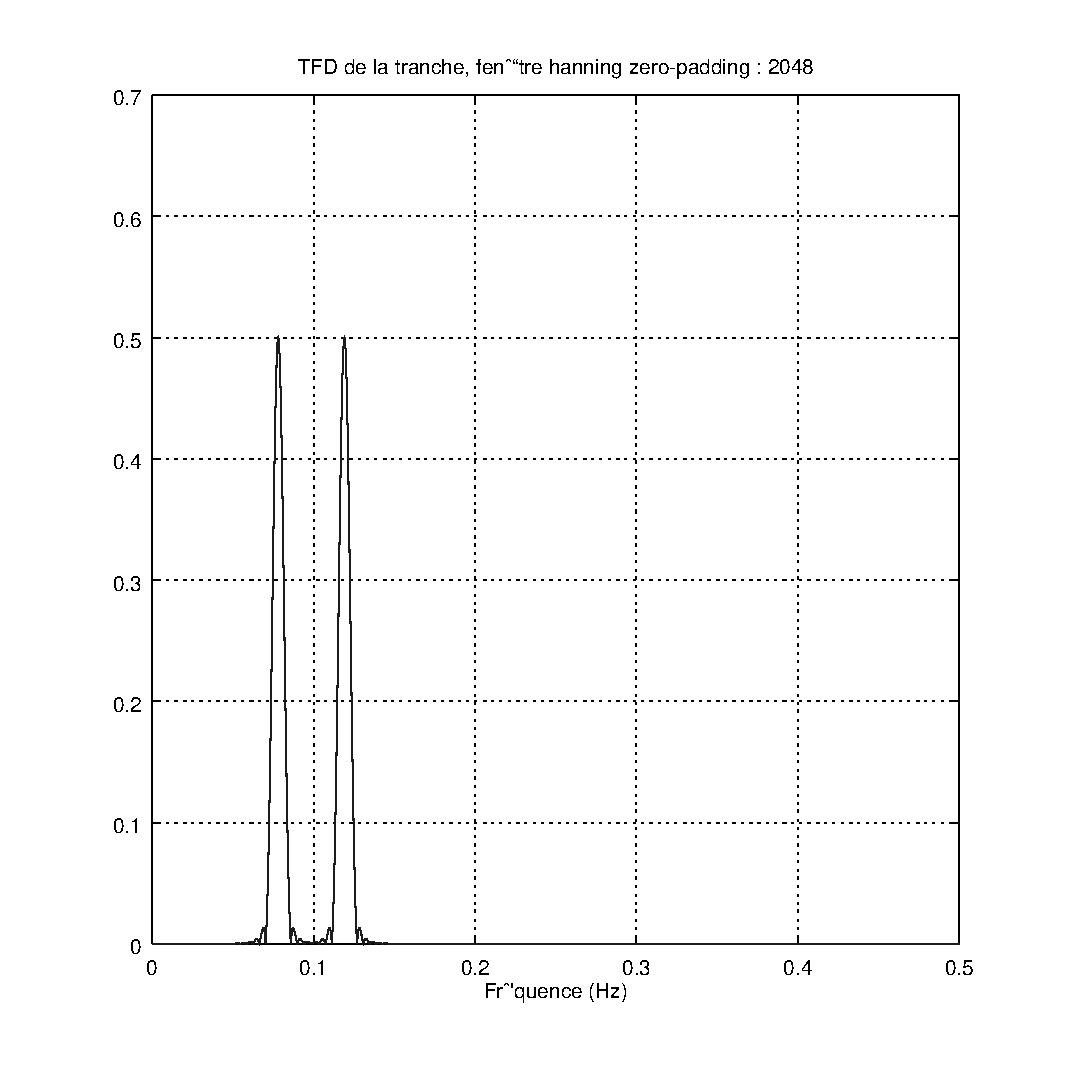
\includegraphics[width=\textwidth]{images/hanning.eps}
  		% Title: glps_renderer figure
% Creator: GL2PS 1.3.8, (C) 1999-2012 C. Geuzaine
% For: Octave
% CreationDate: Wed Nov  8 10:42:42 2017
\begin{pgfpicture}
\pgfsetlinewidth{0.01pt}
\color[rgb]{1.000000,1.000000,1.000000}
\pgfpathmoveto{\pgfpoint{65.000015pt}{104.000000pt}}
\pgflineto{\pgfpoint{452.500031pt}{26.999981pt}}
\pgflineto{\pgfpoint{65.000015pt}{26.999981pt}}
\pgfpathclose
\pgfusepath{fill,stroke}
\pgfpathmoveto{\pgfpoint{65.000015pt}{104.000000pt}}
\pgflineto{\pgfpoint{452.500031pt}{104.000000pt}}
\pgflineto{\pgfpoint{452.500031pt}{26.999981pt}}
\pgfpathclose
\pgfusepath{fill,stroke}
\color[rgb]{0.000000,0.000000,0.000000}
\pgfsetlinewidth{0.500000pt}
\pgfsetdash{{16pt}{0pt}}{0pt}
\pgfpathmoveto{\pgfpoint{452.500031pt}{26.999981pt}}
\pgflineto{\pgfpoint{65.000015pt}{26.999981pt}}
\pgfusepath{stroke}
\pgfpathmoveto{\pgfpoint{452.500031pt}{104.000000pt}}
\pgflineto{\pgfpoint{65.000015pt}{104.000000pt}}
\pgfusepath{stroke}
\pgfpathmoveto{\pgfpoint{65.000015pt}{104.000000pt}}
\pgflineto{\pgfpoint{65.000015pt}{26.999981pt}}
\pgfusepath{stroke}
\pgfpathmoveto{\pgfpoint{452.500031pt}{104.000000pt}}
\pgflineto{\pgfpoint{452.500031pt}{26.999981pt}}
\pgfusepath{stroke}
\pgfsetdash{{0pt}{3pt}{1pt}{3pt}{1pt}{3pt}{1pt}{3pt}{1pt}{0pt}}{0pt}
\pgfpathmoveto{\pgfpoint{65.000015pt}{104.000000pt}}
\pgflineto{\pgfpoint{65.000015pt}{26.999981pt}}
\pgfusepath{stroke}
\pgfpathmoveto{\pgfpoint{142.500031pt}{104.000000pt}}
\pgflineto{\pgfpoint{142.500031pt}{26.999981pt}}
\pgfusepath{stroke}
\pgfpathmoveto{\pgfpoint{220.000031pt}{104.000000pt}}
\pgflineto{\pgfpoint{220.000031pt}{26.999981pt}}
\pgfusepath{stroke}
\pgfpathmoveto{\pgfpoint{297.500031pt}{104.000000pt}}
\pgflineto{\pgfpoint{297.500031pt}{26.999981pt}}
\pgfusepath{stroke}
\pgfpathmoveto{\pgfpoint{375.000061pt}{104.000000pt}}
\pgflineto{\pgfpoint{375.000061pt}{26.999981pt}}
\pgfusepath{stroke}
\pgfpathmoveto{\pgfpoint{452.500031pt}{104.000000pt}}
\pgflineto{\pgfpoint{452.500031pt}{26.999981pt}}
\pgfusepath{stroke}
\pgfsetdash{{16pt}{0pt}}{0pt}
\pgfpathmoveto{\pgfpoint{65.000015pt}{30.874983pt}}
\pgflineto{\pgfpoint{65.000015pt}{26.999981pt}}
\pgfusepath{stroke}
\pgfpathmoveto{\pgfpoint{65.000015pt}{100.125008pt}}
\pgflineto{\pgfpoint{65.000015pt}{104.000000pt}}
\pgfusepath{stroke}
\pgfpathmoveto{\pgfpoint{142.500031pt}{30.874983pt}}
\pgflineto{\pgfpoint{142.500031pt}{26.999981pt}}
\pgfusepath{stroke}
\pgfpathmoveto{\pgfpoint{142.500031pt}{100.125008pt}}
\pgflineto{\pgfpoint{142.500031pt}{104.000000pt}}
\pgfusepath{stroke}
\pgfpathmoveto{\pgfpoint{220.000031pt}{30.874983pt}}
\pgflineto{\pgfpoint{220.000031pt}{26.999981pt}}
\pgfusepath{stroke}
\pgfpathmoveto{\pgfpoint{220.000031pt}{100.125008pt}}
\pgflineto{\pgfpoint{220.000031pt}{104.000000pt}}
\pgfusepath{stroke}
\pgfpathmoveto{\pgfpoint{297.500031pt}{30.874983pt}}
\pgflineto{\pgfpoint{297.500031pt}{26.999981pt}}
\pgfusepath{stroke}
\pgfpathmoveto{\pgfpoint{297.500031pt}{100.125008pt}}
\pgflineto{\pgfpoint{297.500031pt}{104.000000pt}}
\pgfusepath{stroke}
\pgfpathmoveto{\pgfpoint{375.000061pt}{30.874983pt}}
\pgflineto{\pgfpoint{375.000061pt}{26.999981pt}}
\pgfusepath{stroke}
\pgfpathmoveto{\pgfpoint{375.000061pt}{100.125008pt}}
\pgflineto{\pgfpoint{375.000061pt}{104.000000pt}}
\pgfusepath{stroke}
\pgfpathmoveto{\pgfpoint{452.500031pt}{30.874983pt}}
\pgflineto{\pgfpoint{452.500031pt}{26.999981pt}}
\pgfusepath{stroke}
\pgfpathmoveto{\pgfpoint{452.500031pt}{100.125008pt}}
\pgflineto{\pgfpoint{452.500031pt}{104.000000pt}}
\pgfusepath{stroke}
{
\pgftransformshift{\pgfpoint{65.000015pt}{21.999977pt}}
\pgfnode{rectangle}{north}{\fontsize{10}{0}\selectfont\textcolor[rgb]{0,0,0}{{0}}}{}{\pgfusepath{discard}}}
{
\pgftransformshift{\pgfpoint{142.500015pt}{21.999977pt}}
\pgfnode{rectangle}{north}{\fontsize{10}{0}\selectfont\textcolor[rgb]{0,0,0}{{0.1}}}{}{\pgfusepath{discard}}}
{
\pgftransformshift{\pgfpoint{220.000015pt}{21.999977pt}}
\pgfnode{rectangle}{north}{\fontsize{10}{0}\selectfont\textcolor[rgb]{0,0,0}{{0.2}}}{}{\pgfusepath{discard}}}
{
\pgftransformshift{\pgfpoint{297.500031pt}{21.999977pt}}
\pgfnode{rectangle}{north}{\fontsize{10}{0}\selectfont\textcolor[rgb]{0,0,0}{{0.3}}}{}{\pgfusepath{discard}}}
{
\pgftransformshift{\pgfpoint{375.000031pt}{21.999977pt}}
\pgfnode{rectangle}{north}{\fontsize{10}{0}\selectfont\textcolor[rgb]{0,0,0}{{0.4}}}{}{\pgfusepath{discard}}}
{
\pgftransformshift{\pgfpoint{452.500031pt}{21.999977pt}}
\pgfnode{rectangle}{north}{\fontsize{10}{0}\selectfont\textcolor[rgb]{0,0,0}{{0.5}}}{}{\pgfusepath{discard}}}
\pgfsetdash{{0pt}{3pt}{1pt}{3pt}{1pt}{3pt}{1pt}{3pt}{1pt}{0pt}}{0pt}
\pgfpathmoveto{\pgfpoint{452.500031pt}{26.999981pt}}
\pgflineto{\pgfpoint{65.000015pt}{26.999981pt}}
\pgfusepath{stroke}
\pgfpathmoveto{\pgfpoint{452.500031pt}{37.999985pt}}
\pgflineto{\pgfpoint{65.000015pt}{37.999985pt}}
\pgfusepath{stroke}
\pgfpathmoveto{\pgfpoint{452.500031pt}{48.999989pt}}
\pgflineto{\pgfpoint{65.000015pt}{48.999989pt}}
\pgfusepath{stroke}
\pgfpathmoveto{\pgfpoint{452.500031pt}{59.999992pt}}
\pgflineto{\pgfpoint{65.000015pt}{59.999992pt}}
\pgfusepath{stroke}
\pgfpathmoveto{\pgfpoint{452.500031pt}{70.999992pt}}
\pgflineto{\pgfpoint{65.000015pt}{70.999992pt}}
\pgfusepath{stroke}
\pgfpathmoveto{\pgfpoint{452.500031pt}{82.000000pt}}
\pgflineto{\pgfpoint{65.000015pt}{82.000000pt}}
\pgfusepath{stroke}
\pgfpathmoveto{\pgfpoint{452.500031pt}{93.000000pt}}
\pgflineto{\pgfpoint{65.000015pt}{93.000000pt}}
\pgfusepath{stroke}
\pgfpathmoveto{\pgfpoint{452.500031pt}{104.000000pt}}
\pgflineto{\pgfpoint{65.000015pt}{104.000000pt}}
\pgfusepath{stroke}
\pgfsetdash{{16pt}{0pt}}{0pt}
\pgfpathmoveto{\pgfpoint{68.870026pt}{26.999981pt}}
\pgflineto{\pgfpoint{65.000015pt}{26.999981pt}}
\pgfusepath{stroke}
\pgfpathmoveto{\pgfpoint{448.630005pt}{26.999981pt}}
\pgflineto{\pgfpoint{452.500031pt}{26.999981pt}}
\pgfusepath{stroke}
\pgfpathmoveto{\pgfpoint{68.870026pt}{37.999985pt}}
\pgflineto{\pgfpoint{65.000015pt}{37.999985pt}}
\pgfusepath{stroke}
\pgfpathmoveto{\pgfpoint{448.630005pt}{37.999985pt}}
\pgflineto{\pgfpoint{452.500031pt}{37.999985pt}}
\pgfusepath{stroke}
\pgfpathmoveto{\pgfpoint{68.870026pt}{48.999989pt}}
\pgflineto{\pgfpoint{65.000015pt}{48.999989pt}}
\pgfusepath{stroke}
\pgfpathmoveto{\pgfpoint{448.630005pt}{48.999989pt}}
\pgflineto{\pgfpoint{452.500031pt}{48.999989pt}}
\pgfusepath{stroke}
\pgfpathmoveto{\pgfpoint{68.870026pt}{59.999992pt}}
\pgflineto{\pgfpoint{65.000015pt}{59.999992pt}}
\pgfusepath{stroke}
\pgfpathmoveto{\pgfpoint{448.630005pt}{59.999992pt}}
\pgflineto{\pgfpoint{452.500031pt}{59.999992pt}}
\pgfusepath{stroke}
\pgfpathmoveto{\pgfpoint{68.870026pt}{70.999992pt}}
\pgflineto{\pgfpoint{65.000015pt}{70.999992pt}}
\pgfusepath{stroke}
\pgfpathmoveto{\pgfpoint{448.630005pt}{70.999992pt}}
\pgflineto{\pgfpoint{452.500031pt}{70.999992pt}}
\pgfusepath{stroke}
\pgfpathmoveto{\pgfpoint{68.870026pt}{82.000000pt}}
\pgflineto{\pgfpoint{65.000015pt}{82.000000pt}}
\pgfusepath{stroke}
\pgfpathmoveto{\pgfpoint{448.630005pt}{82.000000pt}}
\pgflineto{\pgfpoint{452.500031pt}{82.000000pt}}
\pgfusepath{stroke}
\pgfpathmoveto{\pgfpoint{68.870026pt}{93.000000pt}}
\pgflineto{\pgfpoint{65.000015pt}{93.000000pt}}
\pgfusepath{stroke}
\pgfpathmoveto{\pgfpoint{448.630005pt}{93.000000pt}}
\pgflineto{\pgfpoint{452.500031pt}{93.000000pt}}
\pgfusepath{stroke}
\pgfpathmoveto{\pgfpoint{68.870026pt}{104.000000pt}}
\pgflineto{\pgfpoint{65.000015pt}{104.000000pt}}
\pgfusepath{stroke}
\pgfpathmoveto{\pgfpoint{448.630005pt}{104.000000pt}}
\pgflineto{\pgfpoint{452.500031pt}{104.000000pt}}
\pgfusepath{stroke}
{
\pgftransformshift{\pgfpoint{60.006454pt}{26.999981pt}}
\pgfnode{rectangle}{east}{\fontsize{10}{0}\selectfont\textcolor[rgb]{0,0,0}{{0}}}{}{\pgfusepath{discard}}}
{
\pgftransformshift{\pgfpoint{60.006454pt}{37.999985pt}}
\pgfnode{rectangle}{east}{\fontsize{10}{0}\selectfont\textcolor[rgb]{0,0,0}{{0.1}}}{}{\pgfusepath{discard}}}
{
\pgftransformshift{\pgfpoint{60.006454pt}{48.999989pt}}
\pgfnode{rectangle}{east}{\fontsize{10}{0}\selectfont\textcolor[rgb]{0,0,0}{{0.2}}}{}{\pgfusepath{discard}}}
{
\pgftransformshift{\pgfpoint{60.006454pt}{59.999992pt}}
\pgfnode{rectangle}{east}{\fontsize{10}{0}\selectfont\textcolor[rgb]{0,0,0}{{0.3}}}{}{\pgfusepath{discard}}}
{
\pgftransformshift{\pgfpoint{60.006454pt}{70.999992pt}}
\pgfnode{rectangle}{east}{\fontsize{10}{0}\selectfont\textcolor[rgb]{0,0,0}{{0.4}}}{}{\pgfusepath{discard}}}
{
\pgftransformshift{\pgfpoint{60.006454pt}{82.000000pt}}
\pgfnode{rectangle}{east}{\fontsize{10}{0}\selectfont\textcolor[rgb]{0,0,0}{{0.5}}}{}{\pgfusepath{discard}}}
{
\pgftransformshift{\pgfpoint{60.006454pt}{93.000000pt}}
\pgfnode{rectangle}{east}{\fontsize{10}{0}\selectfont\textcolor[rgb]{0,0,0}{{0.6}}}{}{\pgfusepath{discard}}}
{
\pgftransformshift{\pgfpoint{60.006454pt}{104.000000pt}}
\pgfnode{rectangle}{east}{\fontsize{10}{0}\selectfont\textcolor[rgb]{0,0,0}{{0.7}}}{}{\pgfusepath{discard}}}
{
\pgftransformshift{\pgfpoint{258.750031pt}{10.999977pt}}
\pgfnode{rectangle}{north}{\fontsize{10}{0}\selectfont\textcolor[rgb]{0,0,0}{{Fréquence (Hz)}}}{}{\pgfusepath{discard}}}
\color[rgb]{0.000000,0.000000,1.000000}
\pgfsetdash{}{0pt}
\pgfpathmoveto{\pgfpoint{65.189224pt}{27.001183pt}}
\pgflineto{\pgfpoint{65.000015pt}{27.001171pt}}
\pgfusepath{stroke}
\pgfpathmoveto{\pgfpoint{65.378433pt}{27.001213pt}}
\pgflineto{\pgfpoint{65.189224pt}{27.001183pt}}
\pgfusepath{stroke}
\pgfpathmoveto{\pgfpoint{65.567642pt}{27.001251pt}}
\pgflineto{\pgfpoint{65.378433pt}{27.001213pt}}
\pgfusepath{stroke}
\pgfpathmoveto{\pgfpoint{65.756836pt}{27.001293pt}}
\pgflineto{\pgfpoint{65.567642pt}{27.001251pt}}
\pgfusepath{stroke}
\pgfpathmoveto{\pgfpoint{65.946060pt}{27.001320pt}}
\pgflineto{\pgfpoint{65.756836pt}{27.001293pt}}
\pgfusepath{stroke}
\pgfpathmoveto{\pgfpoint{66.135269pt}{27.001335pt}}
\pgflineto{\pgfpoint{65.946060pt}{27.001320pt}}
\pgfusepath{stroke}
\pgfpathmoveto{\pgfpoint{66.324478pt}{27.001328pt}}
\pgflineto{\pgfpoint{66.135269pt}{27.001335pt}}
\pgfusepath{stroke}
\pgfpathmoveto{\pgfpoint{66.513687pt}{27.001297pt}}
\pgflineto{\pgfpoint{66.324478pt}{27.001328pt}}
\pgfusepath{stroke}
\pgfpathmoveto{\pgfpoint{66.702881pt}{27.001244pt}}
\pgflineto{\pgfpoint{66.513687pt}{27.001297pt}}
\pgfusepath{stroke}
\pgfpathmoveto{\pgfpoint{66.892105pt}{27.001175pt}}
\pgflineto{\pgfpoint{66.702881pt}{27.001244pt}}
\pgfusepath{stroke}
\pgfpathmoveto{\pgfpoint{67.081314pt}{27.001102pt}}
\pgflineto{\pgfpoint{66.892105pt}{27.001175pt}}
\pgfusepath{stroke}
\pgfpathmoveto{\pgfpoint{67.270523pt}{27.001034pt}}
\pgflineto{\pgfpoint{67.081314pt}{27.001102pt}}
\pgfusepath{stroke}
\pgfpathmoveto{\pgfpoint{67.459732pt}{27.000999pt}}
\pgflineto{\pgfpoint{67.270523pt}{27.001034pt}}
\pgfusepath{stroke}
\pgfpathmoveto{\pgfpoint{67.648926pt}{27.001015pt}}
\pgflineto{\pgfpoint{67.459732pt}{27.000999pt}}
\pgfusepath{stroke}
\pgfpathmoveto{\pgfpoint{67.838150pt}{27.001076pt}}
\pgflineto{\pgfpoint{67.648926pt}{27.001015pt}}
\pgfusepath{stroke}
\pgfpathmoveto{\pgfpoint{68.027359pt}{27.001179pt}}
\pgflineto{\pgfpoint{67.838150pt}{27.001076pt}}
\pgfusepath{stroke}
\pgfpathmoveto{\pgfpoint{68.216568pt}{27.001308pt}}
\pgflineto{\pgfpoint{68.027359pt}{27.001179pt}}
\pgfusepath{stroke}
\pgfpathmoveto{\pgfpoint{68.405777pt}{27.001442pt}}
\pgflineto{\pgfpoint{68.216568pt}{27.001308pt}}
\pgfusepath{stroke}
\pgfpathmoveto{\pgfpoint{68.594971pt}{27.001564pt}}
\pgflineto{\pgfpoint{68.405777pt}{27.001442pt}}
\pgfusepath{stroke}
\pgfpathmoveto{\pgfpoint{68.784195pt}{27.001656pt}}
\pgflineto{\pgfpoint{68.594971pt}{27.001564pt}}
\pgfusepath{stroke}
\pgfpathmoveto{\pgfpoint{68.973404pt}{27.001713pt}}
\pgflineto{\pgfpoint{68.784195pt}{27.001656pt}}
\pgfusepath{stroke}
\pgfpathmoveto{\pgfpoint{69.162613pt}{27.001728pt}}
\pgflineto{\pgfpoint{68.973404pt}{27.001713pt}}
\pgfusepath{stroke}
\pgfpathmoveto{\pgfpoint{69.351822pt}{27.001694pt}}
\pgflineto{\pgfpoint{69.162613pt}{27.001728pt}}
\pgfusepath{stroke}
\pgfpathmoveto{\pgfpoint{69.541016pt}{27.001614pt}}
\pgflineto{\pgfpoint{69.351822pt}{27.001694pt}}
\pgfusepath{stroke}
\pgfpathmoveto{\pgfpoint{69.730240pt}{27.001484pt}}
\pgflineto{\pgfpoint{69.541016pt}{27.001614pt}}
\pgfusepath{stroke}
\pgfpathmoveto{\pgfpoint{69.919449pt}{27.001320pt}}
\pgflineto{\pgfpoint{69.730240pt}{27.001484pt}}
\pgfusepath{stroke}
\pgfpathmoveto{\pgfpoint{70.108658pt}{27.001141pt}}
\pgflineto{\pgfpoint{69.919449pt}{27.001320pt}}
\pgfusepath{stroke}
\pgfpathmoveto{\pgfpoint{70.297867pt}{27.000965pt}}
\pgflineto{\pgfpoint{70.108658pt}{27.001141pt}}
\pgfusepath{stroke}
\pgfpathmoveto{\pgfpoint{70.487061pt}{27.000847pt}}
\pgflineto{\pgfpoint{70.297867pt}{27.000965pt}}
\pgfusepath{stroke}
\pgfpathmoveto{\pgfpoint{70.676285pt}{27.000851pt}}
\pgflineto{\pgfpoint{70.487061pt}{27.000847pt}}
\pgfusepath{stroke}
\pgfpathmoveto{\pgfpoint{70.865494pt}{27.000984pt}}
\pgflineto{\pgfpoint{70.676285pt}{27.000851pt}}
\pgfusepath{stroke}
\pgfpathmoveto{\pgfpoint{71.054703pt}{27.001205pt}}
\pgflineto{\pgfpoint{70.865494pt}{27.000984pt}}
\pgfusepath{stroke}
\pgfpathmoveto{\pgfpoint{71.243912pt}{27.001461pt}}
\pgflineto{\pgfpoint{71.054703pt}{27.001205pt}}
\pgfusepath{stroke}
\pgfpathmoveto{\pgfpoint{71.433105pt}{27.001709pt}}
\pgflineto{\pgfpoint{71.243912pt}{27.001461pt}}
\pgfusepath{stroke}
\pgfpathmoveto{\pgfpoint{71.622330pt}{27.001934pt}}
\pgflineto{\pgfpoint{71.433105pt}{27.001709pt}}
\pgfusepath{stroke}
\pgfpathmoveto{\pgfpoint{71.811539pt}{27.002106pt}}
\pgflineto{\pgfpoint{71.622330pt}{27.001934pt}}
\pgfusepath{stroke}
\pgfpathmoveto{\pgfpoint{72.000748pt}{27.002228pt}}
\pgflineto{\pgfpoint{71.811539pt}{27.002106pt}}
\pgfusepath{stroke}
\pgfpathmoveto{\pgfpoint{72.189957pt}{27.002274pt}}
\pgflineto{\pgfpoint{72.000748pt}{27.002228pt}}
\pgfusepath{stroke}
\pgfpathmoveto{\pgfpoint{72.379150pt}{27.002254pt}}
\pgflineto{\pgfpoint{72.189957pt}{27.002274pt}}
\pgfusepath{stroke}
\pgfpathmoveto{\pgfpoint{72.568375pt}{27.002151pt}}
\pgflineto{\pgfpoint{72.379150pt}{27.002254pt}}
\pgfusepath{stroke}
\pgfpathmoveto{\pgfpoint{72.757584pt}{27.001980pt}}
\pgflineto{\pgfpoint{72.568375pt}{27.002151pt}}
\pgfusepath{stroke}
\pgfpathmoveto{\pgfpoint{72.946793pt}{27.001740pt}}
\pgflineto{\pgfpoint{72.757584pt}{27.001980pt}}
\pgfusepath{stroke}
\pgfpathmoveto{\pgfpoint{73.136002pt}{27.001450pt}}
\pgflineto{\pgfpoint{72.946793pt}{27.001740pt}}
\pgfusepath{stroke}
\pgfpathmoveto{\pgfpoint{73.325195pt}{27.001133pt}}
\pgflineto{\pgfpoint{73.136002pt}{27.001450pt}}
\pgfusepath{stroke}
\pgfpathmoveto{\pgfpoint{73.514420pt}{27.000851pt}}
\pgflineto{\pgfpoint{73.325195pt}{27.001133pt}}
\pgfusepath{stroke}
\pgfpathmoveto{\pgfpoint{73.703629pt}{27.000740pt}}
\pgflineto{\pgfpoint{73.514420pt}{27.000851pt}}
\pgfusepath{stroke}
\pgfpathmoveto{\pgfpoint{73.892838pt}{27.000908pt}}
\pgflineto{\pgfpoint{73.703629pt}{27.000740pt}}
\pgfusepath{stroke}
\pgfpathmoveto{\pgfpoint{74.082047pt}{27.001247pt}}
\pgflineto{\pgfpoint{73.892838pt}{27.000908pt}}
\pgfusepath{stroke}
\pgfpathmoveto{\pgfpoint{74.271240pt}{27.001640pt}}
\pgflineto{\pgfpoint{74.082047pt}{27.001247pt}}
\pgfusepath{stroke}
\pgfpathmoveto{\pgfpoint{74.460464pt}{27.002029pt}}
\pgflineto{\pgfpoint{74.271240pt}{27.001640pt}}
\pgfusepath{stroke}
\pgfpathmoveto{\pgfpoint{74.649673pt}{27.002373pt}}
\pgflineto{\pgfpoint{74.460464pt}{27.002029pt}}
\pgfusepath{stroke}
\pgfpathmoveto{\pgfpoint{74.838882pt}{27.002655pt}}
\pgflineto{\pgfpoint{74.649673pt}{27.002373pt}}
\pgfusepath{stroke}
\pgfpathmoveto{\pgfpoint{75.028091pt}{27.002857pt}}
\pgflineto{\pgfpoint{74.838882pt}{27.002655pt}}
\pgfusepath{stroke}
\pgfpathmoveto{\pgfpoint{75.217285pt}{27.002960pt}}
\pgflineto{\pgfpoint{75.028091pt}{27.002857pt}}
\pgfusepath{stroke}
\pgfpathmoveto{\pgfpoint{75.406509pt}{27.002968pt}}
\pgflineto{\pgfpoint{75.217285pt}{27.002960pt}}
\pgfusepath{stroke}
\pgfpathmoveto{\pgfpoint{75.595718pt}{27.002869pt}}
\pgflineto{\pgfpoint{75.406509pt}{27.002968pt}}
\pgfusepath{stroke}
\pgfpathmoveto{\pgfpoint{75.784927pt}{27.002663pt}}
\pgflineto{\pgfpoint{75.595718pt}{27.002869pt}}
\pgfusepath{stroke}
\pgfpathmoveto{\pgfpoint{75.974136pt}{27.002357pt}}
\pgflineto{\pgfpoint{75.784927pt}{27.002663pt}}
\pgfusepath{stroke}
\pgfpathmoveto{\pgfpoint{76.163330pt}{27.001968pt}}
\pgflineto{\pgfpoint{75.974136pt}{27.002357pt}}
\pgfusepath{stroke}
\pgfpathmoveto{\pgfpoint{76.352554pt}{27.001514pt}}
\pgflineto{\pgfpoint{76.163330pt}{27.001968pt}}
\pgfusepath{stroke}
\pgfpathmoveto{\pgfpoint{76.541763pt}{27.001049pt}}
\pgflineto{\pgfpoint{76.352554pt}{27.001514pt}}
\pgfusepath{stroke}
\pgfpathmoveto{\pgfpoint{76.730972pt}{27.000721pt}}
\pgflineto{\pgfpoint{76.541763pt}{27.001049pt}}
\pgfusepath{stroke}
\pgfpathmoveto{\pgfpoint{76.920181pt}{27.000839pt}}
\pgflineto{\pgfpoint{76.730972pt}{27.000721pt}}
\pgfusepath{stroke}
\pgfpathmoveto{\pgfpoint{77.109375pt}{27.001308pt}}
\pgflineto{\pgfpoint{76.920181pt}{27.000839pt}}
\pgfusepath{stroke}
\pgfpathmoveto{\pgfpoint{77.298599pt}{27.001865pt}}
\pgflineto{\pgfpoint{77.109375pt}{27.001308pt}}
\pgfusepath{stroke}
\pgfpathmoveto{\pgfpoint{77.487808pt}{27.002415pt}}
\pgflineto{\pgfpoint{77.298599pt}{27.001865pt}}
\pgfusepath{stroke}
\pgfpathmoveto{\pgfpoint{77.677017pt}{27.002907pt}}
\pgflineto{\pgfpoint{77.487808pt}{27.002415pt}}
\pgfusepath{stroke}
\pgfpathmoveto{\pgfpoint{77.866226pt}{27.003319pt}}
\pgflineto{\pgfpoint{77.677017pt}{27.002907pt}}
\pgfusepath{stroke}
\pgfpathmoveto{\pgfpoint{78.055420pt}{27.003624pt}}
\pgflineto{\pgfpoint{77.866226pt}{27.003319pt}}
\pgfusepath{stroke}
\pgfpathmoveto{\pgfpoint{78.244644pt}{27.003811pt}}
\pgflineto{\pgfpoint{78.055420pt}{27.003624pt}}
\pgfusepath{stroke}
\pgfpathmoveto{\pgfpoint{78.433853pt}{27.003857pt}}
\pgflineto{\pgfpoint{78.244644pt}{27.003811pt}}
\pgfusepath{stroke}
\pgfpathmoveto{\pgfpoint{78.623062pt}{27.003769pt}}
\pgflineto{\pgfpoint{78.433853pt}{27.003857pt}}
\pgfusepath{stroke}
\pgfpathmoveto{\pgfpoint{78.812271pt}{27.003536pt}}
\pgflineto{\pgfpoint{78.623062pt}{27.003769pt}}
\pgfusepath{stroke}
\pgfpathmoveto{\pgfpoint{79.001465pt}{27.003170pt}}
\pgflineto{\pgfpoint{78.812271pt}{27.003536pt}}
\pgfusepath{stroke}
\pgfpathmoveto{\pgfpoint{79.190689pt}{27.002678pt}}
\pgflineto{\pgfpoint{79.001465pt}{27.003170pt}}
\pgfusepath{stroke}
\pgfpathmoveto{\pgfpoint{79.379898pt}{27.002087pt}}
\pgflineto{\pgfpoint{79.190689pt}{27.002678pt}}
\pgfusepath{stroke}
\pgfpathmoveto{\pgfpoint{79.569107pt}{27.001431pt}}
\pgflineto{\pgfpoint{79.379898pt}{27.002087pt}}
\pgfusepath{stroke}
\pgfpathmoveto{\pgfpoint{79.758316pt}{27.000835pt}}
\pgflineto{\pgfpoint{79.569107pt}{27.001431pt}}
\pgfusepath{stroke}
\pgfpathmoveto{\pgfpoint{79.947510pt}{27.000790pt}}
\pgflineto{\pgfpoint{79.758316pt}{27.000835pt}}
\pgfusepath{stroke}
\pgfpathmoveto{\pgfpoint{80.136734pt}{27.001389pt}}
\pgflineto{\pgfpoint{79.947510pt}{27.000790pt}}
\pgfusepath{stroke}
\pgfpathmoveto{\pgfpoint{80.325943pt}{27.002144pt}}
\pgflineto{\pgfpoint{80.136734pt}{27.001389pt}}
\pgfusepath{stroke}
\pgfpathmoveto{\pgfpoint{80.515152pt}{27.002892pt}}
\pgflineto{\pgfpoint{80.325943pt}{27.002144pt}}
\pgfusepath{stroke}
\pgfpathmoveto{\pgfpoint{80.704361pt}{27.003567pt}}
\pgflineto{\pgfpoint{80.515152pt}{27.002892pt}}
\pgfusepath{stroke}
\pgfpathmoveto{\pgfpoint{80.893570pt}{27.004143pt}}
\pgflineto{\pgfpoint{80.704361pt}{27.003567pt}}
\pgfusepath{stroke}
\pgfpathmoveto{\pgfpoint{81.082779pt}{27.004581pt}}
\pgflineto{\pgfpoint{80.893570pt}{27.004143pt}}
\pgfusepath{stroke}
\pgfpathmoveto{\pgfpoint{81.271988pt}{27.004868pt}}
\pgflineto{\pgfpoint{81.082779pt}{27.004581pt}}
\pgfusepath{stroke}
\pgfpathmoveto{\pgfpoint{81.461197pt}{27.004978pt}}
\pgflineto{\pgfpoint{81.271988pt}{27.004868pt}}
\pgfusepath{stroke}
\pgfpathmoveto{\pgfpoint{81.650406pt}{27.004906pt}}
\pgflineto{\pgfpoint{81.461197pt}{27.004978pt}}
\pgfusepath{stroke}
\pgfpathmoveto{\pgfpoint{81.839615pt}{27.004646pt}}
\pgflineto{\pgfpoint{81.650406pt}{27.004906pt}}
\pgfusepath{stroke}
\pgfpathmoveto{\pgfpoint{82.028824pt}{27.004208pt}}
\pgflineto{\pgfpoint{81.839615pt}{27.004646pt}}
\pgfusepath{stroke}
\pgfpathmoveto{\pgfpoint{82.218033pt}{27.003601pt}}
\pgflineto{\pgfpoint{82.028824pt}{27.004208pt}}
\pgfusepath{stroke}
\pgfpathmoveto{\pgfpoint{82.407242pt}{27.002850pt}}
\pgflineto{\pgfpoint{82.218033pt}{27.003601pt}}
\pgfusepath{stroke}
\pgfpathmoveto{\pgfpoint{82.596451pt}{27.001984pt}}
\pgflineto{\pgfpoint{82.407242pt}{27.002850pt}}
\pgfusepath{stroke}
\pgfpathmoveto{\pgfpoint{82.785660pt}{27.001118pt}}
\pgflineto{\pgfpoint{82.596451pt}{27.001984pt}}
\pgfusepath{stroke}
\pgfpathmoveto{\pgfpoint{82.974869pt}{27.000759pt}}
\pgflineto{\pgfpoint{82.785660pt}{27.001118pt}}
\pgfusepath{stroke}
\pgfpathmoveto{\pgfpoint{83.164078pt}{27.001495pt}}
\pgflineto{\pgfpoint{82.974869pt}{27.000759pt}}
\pgfusepath{stroke}
\pgfpathmoveto{\pgfpoint{83.353287pt}{27.002495pt}}
\pgflineto{\pgfpoint{83.164078pt}{27.001495pt}}
\pgfusepath{stroke}
\pgfpathmoveto{\pgfpoint{83.542496pt}{27.003490pt}}
\pgflineto{\pgfpoint{83.353287pt}{27.002495pt}}
\pgfusepath{stroke}
\pgfpathmoveto{\pgfpoint{83.731705pt}{27.004402pt}}
\pgflineto{\pgfpoint{83.542496pt}{27.003490pt}}
\pgfusepath{stroke}
\pgfpathmoveto{\pgfpoint{83.920914pt}{27.005188pt}}
\pgflineto{\pgfpoint{83.731705pt}{27.004402pt}}
\pgfusepath{stroke}
\pgfpathmoveto{\pgfpoint{84.110123pt}{27.005802pt}}
\pgflineto{\pgfpoint{83.920914pt}{27.005188pt}}
\pgfusepath{stroke}
\pgfpathmoveto{\pgfpoint{84.299332pt}{27.006222pt}}
\pgflineto{\pgfpoint{84.110123pt}{27.005802pt}}
\pgfusepath{stroke}
\pgfpathmoveto{\pgfpoint{84.488541pt}{27.006413pt}}
\pgflineto{\pgfpoint{84.299332pt}{27.006222pt}}
\pgfusepath{stroke}
\pgfpathmoveto{\pgfpoint{84.677750pt}{27.006374pt}}
\pgflineto{\pgfpoint{84.488541pt}{27.006413pt}}
\pgfusepath{stroke}
\pgfpathmoveto{\pgfpoint{84.866959pt}{27.006088pt}}
\pgflineto{\pgfpoint{84.677750pt}{27.006374pt}}
\pgfusepath{stroke}
\pgfpathmoveto{\pgfpoint{85.056168pt}{27.005566pt}}
\pgflineto{\pgfpoint{84.866959pt}{27.006088pt}}
\pgfusepath{stroke}
\pgfpathmoveto{\pgfpoint{85.245377pt}{27.004810pt}}
\pgflineto{\pgfpoint{85.056168pt}{27.005566pt}}
\pgfusepath{stroke}
\pgfpathmoveto{\pgfpoint{85.434586pt}{27.003860pt}}
\pgflineto{\pgfpoint{85.245377pt}{27.004810pt}}
\pgfusepath{stroke}
\pgfpathmoveto{\pgfpoint{85.623795pt}{27.002750pt}}
\pgflineto{\pgfpoint{85.434586pt}{27.003860pt}}
\pgfusepath{stroke}
\pgfpathmoveto{\pgfpoint{85.813004pt}{27.001564pt}}
\pgflineto{\pgfpoint{85.623795pt}{27.002750pt}}
\pgfusepath{stroke}
\pgfpathmoveto{\pgfpoint{86.002213pt}{27.000782pt}}
\pgflineto{\pgfpoint{85.813004pt}{27.001564pt}}
\pgfusepath{stroke}
\pgfpathmoveto{\pgfpoint{86.191422pt}{27.001625pt}}
\pgflineto{\pgfpoint{86.002213pt}{27.000782pt}}
\pgfusepath{stroke}
\pgfpathmoveto{\pgfpoint{86.380630pt}{27.002949pt}}
\pgflineto{\pgfpoint{86.191422pt}{27.001625pt}}
\pgfusepath{stroke}
\pgfpathmoveto{\pgfpoint{86.569839pt}{27.004269pt}}
\pgflineto{\pgfpoint{86.380630pt}{27.002949pt}}
\pgfusepath{stroke}
\pgfpathmoveto{\pgfpoint{86.759048pt}{27.005489pt}}
\pgflineto{\pgfpoint{86.569839pt}{27.004269pt}}
\pgfusepath{stroke}
\pgfpathmoveto{\pgfpoint{86.948257pt}{27.006550pt}}
\pgflineto{\pgfpoint{86.759048pt}{27.005489pt}}
\pgfusepath{stroke}
\pgfpathmoveto{\pgfpoint{87.137466pt}{27.007401pt}}
\pgflineto{\pgfpoint{86.948257pt}{27.006550pt}}
\pgfusepath{stroke}
\pgfpathmoveto{\pgfpoint{87.326675pt}{27.007996pt}}
\pgflineto{\pgfpoint{87.137466pt}{27.007401pt}}
\pgfusepath{stroke}
\pgfpathmoveto{\pgfpoint{87.515884pt}{27.008308pt}}
\pgflineto{\pgfpoint{87.326675pt}{27.007996pt}}
\pgfusepath{stroke}
\pgfpathmoveto{\pgfpoint{87.705093pt}{27.008312pt}}
\pgflineto{\pgfpoint{87.515884pt}{27.008308pt}}
\pgfusepath{stroke}
\pgfpathmoveto{\pgfpoint{87.894302pt}{27.007999pt}}
\pgflineto{\pgfpoint{87.705093pt}{27.008312pt}}
\pgfusepath{stroke}
\pgfpathmoveto{\pgfpoint{88.083511pt}{27.007370pt}}
\pgflineto{\pgfpoint{87.894302pt}{27.007999pt}}
\pgfusepath{stroke}
\pgfpathmoveto{\pgfpoint{88.272720pt}{27.006439pt}}
\pgflineto{\pgfpoint{88.083511pt}{27.007370pt}}
\pgfusepath{stroke}
\pgfpathmoveto{\pgfpoint{88.461929pt}{27.005238pt}}
\pgflineto{\pgfpoint{88.272720pt}{27.006439pt}}
\pgfusepath{stroke}
\pgfpathmoveto{\pgfpoint{88.651138pt}{27.003803pt}}
\pgflineto{\pgfpoint{88.461929pt}{27.005238pt}}
\pgfusepath{stroke}
\pgfpathmoveto{\pgfpoint{88.840347pt}{27.002228pt}}
\pgflineto{\pgfpoint{88.651138pt}{27.003803pt}}
\pgfusepath{stroke}
\pgfpathmoveto{\pgfpoint{89.029556pt}{27.000900pt}}
\pgflineto{\pgfpoint{88.840347pt}{27.002228pt}}
\pgfusepath{stroke}
\pgfpathmoveto{\pgfpoint{89.218765pt}{27.001789pt}}
\pgflineto{\pgfpoint{89.029556pt}{27.000900pt}}
\pgfusepath{stroke}
\pgfpathmoveto{\pgfpoint{89.407974pt}{27.003540pt}}
\pgflineto{\pgfpoint{89.218765pt}{27.001789pt}}
\pgfusepath{stroke}
\pgfpathmoveto{\pgfpoint{89.597183pt}{27.005302pt}}
\pgflineto{\pgfpoint{89.407974pt}{27.003540pt}}
\pgfusepath{stroke}
\pgfpathmoveto{\pgfpoint{89.786392pt}{27.006947pt}}
\pgflineto{\pgfpoint{89.597183pt}{27.005302pt}}
\pgfusepath{stroke}
\pgfpathmoveto{\pgfpoint{89.975601pt}{27.008385pt}}
\pgflineto{\pgfpoint{89.786392pt}{27.006947pt}}
\pgfusepath{stroke}
\pgfpathmoveto{\pgfpoint{90.164810pt}{27.009560pt}}
\pgflineto{\pgfpoint{89.975601pt}{27.008385pt}}
\pgfusepath{stroke}
\pgfpathmoveto{\pgfpoint{90.354019pt}{27.010403pt}}
\pgflineto{\pgfpoint{90.164810pt}{27.009560pt}}
\pgfusepath{stroke}
\pgfpathmoveto{\pgfpoint{90.543228pt}{27.010880pt}}
\pgflineto{\pgfpoint{90.354019pt}{27.010403pt}}
\pgfusepath{stroke}
\pgfpathmoveto{\pgfpoint{90.732437pt}{27.010960pt}}
\pgflineto{\pgfpoint{90.543228pt}{27.010880pt}}
\pgfusepath{stroke}
\pgfpathmoveto{\pgfpoint{90.921646pt}{27.010616pt}}
\pgflineto{\pgfpoint{90.732437pt}{27.010960pt}}
\pgfusepath{stroke}
\pgfpathmoveto{\pgfpoint{91.110855pt}{27.009853pt}}
\pgflineto{\pgfpoint{90.921646pt}{27.010616pt}}
\pgfusepath{stroke}
\pgfpathmoveto{\pgfpoint{91.300064pt}{27.008682pt}}
\pgflineto{\pgfpoint{91.110855pt}{27.009853pt}}
\pgfusepath{stroke}
\pgfpathmoveto{\pgfpoint{91.489273pt}{27.007141pt}}
\pgflineto{\pgfpoint{91.300064pt}{27.008682pt}}
\pgfusepath{stroke}
\pgfpathmoveto{\pgfpoint{91.678482pt}{27.005280pt}}
\pgflineto{\pgfpoint{91.489273pt}{27.007141pt}}
\pgfusepath{stroke}
\pgfpathmoveto{\pgfpoint{91.867691pt}{27.003189pt}}
\pgflineto{\pgfpoint{91.678482pt}{27.005280pt}}
\pgfusepath{stroke}
\pgfpathmoveto{\pgfpoint{92.056900pt}{27.001183pt}}
\pgflineto{\pgfpoint{91.867691pt}{27.003189pt}}
\pgfusepath{stroke}
\pgfpathmoveto{\pgfpoint{92.246109pt}{27.001995pt}}
\pgflineto{\pgfpoint{92.056900pt}{27.001183pt}}
\pgfusepath{stroke}
\pgfpathmoveto{\pgfpoint{92.435318pt}{27.004341pt}}
\pgflineto{\pgfpoint{92.246109pt}{27.001995pt}}
\pgfusepath{stroke}
\pgfpathmoveto{\pgfpoint{92.624527pt}{27.006718pt}}
\pgflineto{\pgfpoint{92.435318pt}{27.004341pt}}
\pgfusepath{stroke}
\pgfpathmoveto{\pgfpoint{92.813736pt}{27.008949pt}}
\pgflineto{\pgfpoint{92.624527pt}{27.006718pt}}
\pgfusepath{stroke}
\pgfpathmoveto{\pgfpoint{93.002945pt}{27.010925pt}}
\pgflineto{\pgfpoint{92.813736pt}{27.008949pt}}
\pgfusepath{stroke}
\pgfpathmoveto{\pgfpoint{93.192154pt}{27.012558pt}}
\pgflineto{\pgfpoint{93.002945pt}{27.010925pt}}
\pgfusepath{stroke}
\pgfpathmoveto{\pgfpoint{93.381363pt}{27.013767pt}}
\pgflineto{\pgfpoint{93.192154pt}{27.012558pt}}
\pgfusepath{stroke}
\pgfpathmoveto{\pgfpoint{93.570572pt}{27.014492pt}}
\pgflineto{\pgfpoint{93.381363pt}{27.013767pt}}
\pgfusepath{stroke}
\pgfpathmoveto{\pgfpoint{93.759781pt}{27.014679pt}}
\pgflineto{\pgfpoint{93.570572pt}{27.014492pt}}
\pgfusepath{stroke}
\pgfpathmoveto{\pgfpoint{93.948990pt}{27.014309pt}}
\pgflineto{\pgfpoint{93.759781pt}{27.014679pt}}
\pgfusepath{stroke}
\pgfpathmoveto{\pgfpoint{94.138199pt}{27.013371pt}}
\pgflineto{\pgfpoint{93.948990pt}{27.014309pt}}
\pgfusepath{stroke}
\pgfpathmoveto{\pgfpoint{94.327408pt}{27.011879pt}}
\pgflineto{\pgfpoint{94.138199pt}{27.013371pt}}
\pgfusepath{stroke}
\pgfpathmoveto{\pgfpoint{94.516617pt}{27.009876pt}}
\pgflineto{\pgfpoint{94.327408pt}{27.011879pt}}
\pgfusepath{stroke}
\pgfpathmoveto{\pgfpoint{94.705826pt}{27.007420pt}}
\pgflineto{\pgfpoint{94.516617pt}{27.009876pt}}
\pgfusepath{stroke}
\pgfpathmoveto{\pgfpoint{94.895035pt}{27.004612pt}}
\pgflineto{\pgfpoint{94.705826pt}{27.007420pt}}
\pgfusepath{stroke}
\pgfpathmoveto{\pgfpoint{95.084244pt}{27.001724pt}}
\pgflineto{\pgfpoint{94.895035pt}{27.004612pt}}
\pgfusepath{stroke}
\pgfpathmoveto{\pgfpoint{95.273453pt}{27.002251pt}}
\pgflineto{\pgfpoint{95.084244pt}{27.001724pt}}
\pgfusepath{stroke}
\pgfpathmoveto{\pgfpoint{95.462662pt}{27.005455pt}}
\pgflineto{\pgfpoint{95.273453pt}{27.002251pt}}
\pgfusepath{stroke}
\pgfpathmoveto{\pgfpoint{95.651871pt}{27.008724pt}}
\pgflineto{\pgfpoint{95.462662pt}{27.005455pt}}
\pgfusepath{stroke}
\pgfpathmoveto{\pgfpoint{95.841080pt}{27.011806pt}}
\pgflineto{\pgfpoint{95.651871pt}{27.008724pt}}
\pgfusepath{stroke}
\pgfpathmoveto{\pgfpoint{96.030289pt}{27.014572pt}}
\pgflineto{\pgfpoint{95.841080pt}{27.011806pt}}
\pgfusepath{stroke}
\pgfpathmoveto{\pgfpoint{96.219498pt}{27.016880pt}}
\pgflineto{\pgfpoint{96.030289pt}{27.014572pt}}
\pgfusepath{stroke}
\pgfpathmoveto{\pgfpoint{96.408707pt}{27.018635pt}}
\pgflineto{\pgfpoint{96.219498pt}{27.016880pt}}
\pgfusepath{stroke}
\pgfpathmoveto{\pgfpoint{96.597916pt}{27.019737pt}}
\pgflineto{\pgfpoint{96.408707pt}{27.018635pt}}
\pgfusepath{stroke}
\pgfpathmoveto{\pgfpoint{96.787125pt}{27.020119pt}}
\pgflineto{\pgfpoint{96.597916pt}{27.019737pt}}
\pgfusepath{stroke}
\pgfpathmoveto{\pgfpoint{96.976334pt}{27.019733pt}}
\pgflineto{\pgfpoint{96.787125pt}{27.020119pt}}
\pgfusepath{stroke}
\pgfpathmoveto{\pgfpoint{97.165543pt}{27.018559pt}}
\pgflineto{\pgfpoint{96.976334pt}{27.019733pt}}
\pgfusepath{stroke}
\pgfpathmoveto{\pgfpoint{97.354752pt}{27.016617pt}}
\pgflineto{\pgfpoint{97.165543pt}{27.018559pt}}
\pgfusepath{stroke}
\pgfpathmoveto{\pgfpoint{97.543961pt}{27.013947pt}}
\pgflineto{\pgfpoint{97.354752pt}{27.016617pt}}
\pgfusepath{stroke}
\pgfpathmoveto{\pgfpoint{97.733170pt}{27.010632pt}}
\pgflineto{\pgfpoint{97.543961pt}{27.013947pt}}
\pgfusepath{stroke}
\pgfpathmoveto{\pgfpoint{97.922379pt}{27.006779pt}}
\pgflineto{\pgfpoint{97.733170pt}{27.010632pt}}
\pgfusepath{stroke}
\pgfpathmoveto{\pgfpoint{98.111588pt}{27.002659pt}}
\pgflineto{\pgfpoint{97.922379pt}{27.006779pt}}
\pgfusepath{stroke}
\pgfpathmoveto{\pgfpoint{98.300797pt}{27.002563pt}}
\pgflineto{\pgfpoint{98.111588pt}{27.002659pt}}
\pgfusepath{stroke}
\pgfpathmoveto{\pgfpoint{98.490005pt}{27.007061pt}}
\pgflineto{\pgfpoint{98.300797pt}{27.002563pt}}
\pgfusepath{stroke}
\pgfpathmoveto{\pgfpoint{98.679214pt}{27.011669pt}}
\pgflineto{\pgfpoint{98.490005pt}{27.007061pt}}
\pgfusepath{stroke}
\pgfpathmoveto{\pgfpoint{98.868423pt}{27.016060pt}}
\pgflineto{\pgfpoint{98.679214pt}{27.011669pt}}
\pgfusepath{stroke}
\pgfpathmoveto{\pgfpoint{99.057632pt}{27.020031pt}}
\pgflineto{\pgfpoint{98.868423pt}{27.016060pt}}
\pgfusepath{stroke}
\pgfpathmoveto{\pgfpoint{99.246841pt}{27.023396pt}}
\pgflineto{\pgfpoint{99.057632pt}{27.020031pt}}
\pgfusepath{stroke}
\pgfpathmoveto{\pgfpoint{99.436050pt}{27.026005pt}}
\pgflineto{\pgfpoint{99.246841pt}{27.023396pt}}
\pgfusepath{stroke}
\pgfpathmoveto{\pgfpoint{99.625259pt}{27.027718pt}}
\pgflineto{\pgfpoint{99.436050pt}{27.026005pt}}
\pgfusepath{stroke}
\pgfpathmoveto{\pgfpoint{99.814468pt}{27.028423pt}}
\pgflineto{\pgfpoint{99.625259pt}{27.027718pt}}
\pgfusepath{stroke}
\pgfpathmoveto{\pgfpoint{100.003677pt}{27.028049pt}}
\pgflineto{\pgfpoint{99.814468pt}{27.028423pt}}
\pgfusepath{stroke}
\pgfpathmoveto{\pgfpoint{100.192886pt}{27.026562pt}}
\pgflineto{\pgfpoint{100.003677pt}{27.028049pt}}
\pgfusepath{stroke}
\pgfpathmoveto{\pgfpoint{100.382095pt}{27.023960pt}}
\pgflineto{\pgfpoint{100.192886pt}{27.026562pt}}
\pgfusepath{stroke}
\pgfpathmoveto{\pgfpoint{100.571304pt}{27.020302pt}}
\pgflineto{\pgfpoint{100.382095pt}{27.023960pt}}
\pgfusepath{stroke}
\pgfpathmoveto{\pgfpoint{100.760513pt}{27.015682pt}}
\pgflineto{\pgfpoint{100.571304pt}{27.020302pt}}
\pgfusepath{stroke}
\pgfpathmoveto{\pgfpoint{100.949722pt}{27.010242pt}}
\pgflineto{\pgfpoint{100.760513pt}{27.015682pt}}
\pgfusepath{stroke}
\pgfpathmoveto{\pgfpoint{101.138931pt}{27.004261pt}}
\pgflineto{\pgfpoint{100.949722pt}{27.010242pt}}
\pgfusepath{stroke}
\pgfpathmoveto{\pgfpoint{101.328140pt}{27.002953pt}}
\pgflineto{\pgfpoint{101.138931pt}{27.004261pt}}
\pgfusepath{stroke}
\pgfpathmoveto{\pgfpoint{101.517349pt}{27.009495pt}}
\pgflineto{\pgfpoint{101.328140pt}{27.002953pt}}
\pgfusepath{stroke}
\pgfpathmoveto{\pgfpoint{101.706558pt}{27.016239pt}}
\pgflineto{\pgfpoint{101.517349pt}{27.009495pt}}
\pgfusepath{stroke}
\pgfpathmoveto{\pgfpoint{101.895767pt}{27.022713pt}}
\pgflineto{\pgfpoint{101.706558pt}{27.016239pt}}
\pgfusepath{stroke}
\pgfpathmoveto{\pgfpoint{102.084976pt}{27.028629pt}}
\pgflineto{\pgfpoint{101.895767pt}{27.022713pt}}
\pgfusepath{stroke}
\pgfpathmoveto{\pgfpoint{102.274185pt}{27.033726pt}}
\pgflineto{\pgfpoint{102.084976pt}{27.028629pt}}
\pgfusepath{stroke}
\pgfpathmoveto{\pgfpoint{102.463394pt}{27.037754pt}}
\pgflineto{\pgfpoint{102.274185pt}{27.033726pt}}
\pgfusepath{stroke}
\pgfpathmoveto{\pgfpoint{102.652603pt}{27.040508pt}}
\pgflineto{\pgfpoint{102.463394pt}{27.037754pt}}
\pgfusepath{stroke}
\pgfpathmoveto{\pgfpoint{102.841812pt}{27.041809pt}}
\pgflineto{\pgfpoint{102.652603pt}{27.040508pt}}
\pgfusepath{stroke}
\pgfpathmoveto{\pgfpoint{103.031021pt}{27.041527pt}}
\pgflineto{\pgfpoint{102.841812pt}{27.041809pt}}
\pgfusepath{stroke}
\pgfpathmoveto{\pgfpoint{103.220230pt}{27.039597pt}}
\pgflineto{\pgfpoint{103.031021pt}{27.041527pt}}
\pgfusepath{stroke}
\pgfpathmoveto{\pgfpoint{103.409439pt}{27.035999pt}}
\pgflineto{\pgfpoint{103.220230pt}{27.039597pt}}
\pgfusepath{stroke}
\pgfpathmoveto{\pgfpoint{103.598648pt}{27.030792pt}}
\pgflineto{\pgfpoint{103.409439pt}{27.035999pt}}
\pgfusepath{stroke}
\pgfpathmoveto{\pgfpoint{103.787857pt}{27.024086pt}}
\pgflineto{\pgfpoint{103.598648pt}{27.030792pt}}
\pgfusepath{stroke}
\pgfpathmoveto{\pgfpoint{103.977066pt}{27.016083pt}}
\pgflineto{\pgfpoint{103.787857pt}{27.024086pt}}
\pgfusepath{stroke}
\pgfpathmoveto{\pgfpoint{104.166275pt}{27.007092pt}}
\pgflineto{\pgfpoint{103.977066pt}{27.016083pt}}
\pgfusepath{stroke}
\pgfpathmoveto{\pgfpoint{104.355484pt}{27.003441pt}}
\pgflineto{\pgfpoint{104.166275pt}{27.007092pt}}
\pgfusepath{stroke}
\pgfpathmoveto{\pgfpoint{104.544693pt}{27.013420pt}}
\pgflineto{\pgfpoint{104.355484pt}{27.003441pt}}
\pgfusepath{stroke}
\pgfpathmoveto{\pgfpoint{104.733902pt}{27.023766pt}}
\pgflineto{\pgfpoint{104.544693pt}{27.013420pt}}
\pgfusepath{stroke}
\pgfpathmoveto{\pgfpoint{104.923111pt}{27.033794pt}}
\pgflineto{\pgfpoint{104.733902pt}{27.023766pt}}
\pgfusepath{stroke}
\pgfpathmoveto{\pgfpoint{105.112320pt}{27.043076pt}}
\pgflineto{\pgfpoint{104.923111pt}{27.033794pt}}
\pgfusepath{stroke}
\pgfpathmoveto{\pgfpoint{105.301529pt}{27.051197pt}}
\pgflineto{\pgfpoint{105.112320pt}{27.043076pt}}
\pgfusepath{stroke}
\pgfpathmoveto{\pgfpoint{105.490738pt}{27.057758pt}}
\pgflineto{\pgfpoint{105.301529pt}{27.051197pt}}
\pgfusepath{stroke}
\pgfpathmoveto{\pgfpoint{105.679947pt}{27.062424pt}}
\pgflineto{\pgfpoint{105.490738pt}{27.057758pt}}
\pgfusepath{stroke}
\pgfpathmoveto{\pgfpoint{105.869156pt}{27.064888pt}}
\pgflineto{\pgfpoint{105.679947pt}{27.062424pt}}
\pgfusepath{stroke}
\pgfpathmoveto{\pgfpoint{106.058365pt}{27.064919pt}}
\pgflineto{\pgfpoint{105.869156pt}{27.064888pt}}
\pgfusepath{stroke}
\pgfpathmoveto{\pgfpoint{106.247574pt}{27.062370pt}}
\pgflineto{\pgfpoint{106.058365pt}{27.064919pt}}
\pgfusepath{stroke}
\pgfpathmoveto{\pgfpoint{106.436783pt}{27.057178pt}}
\pgflineto{\pgfpoint{106.247574pt}{27.062370pt}}
\pgfusepath{stroke}
\pgfpathmoveto{\pgfpoint{106.625992pt}{27.049385pt}}
\pgflineto{\pgfpoint{106.436783pt}{27.057178pt}}
\pgfusepath{stroke}
\pgfpathmoveto{\pgfpoint{106.815201pt}{27.039131pt}}
\pgflineto{\pgfpoint{106.625992pt}{27.049385pt}}
\pgfusepath{stroke}
\pgfpathmoveto{\pgfpoint{107.004410pt}{27.026672pt}}
\pgflineto{\pgfpoint{106.815201pt}{27.039131pt}}
\pgfusepath{stroke}
\pgfpathmoveto{\pgfpoint{107.193619pt}{27.012413pt}}
\pgflineto{\pgfpoint{107.004410pt}{27.026672pt}}
\pgfusepath{stroke}
\pgfpathmoveto{\pgfpoint{107.382828pt}{27.004063pt}}
\pgflineto{\pgfpoint{107.193619pt}{27.012413pt}}
\pgfusepath{stroke}
\pgfpathmoveto{\pgfpoint{107.572037pt}{27.020294pt}}
\pgflineto{\pgfpoint{107.382828pt}{27.004063pt}}
\pgfusepath{stroke}
\pgfpathmoveto{\pgfpoint{107.761246pt}{27.037239pt}}
\pgflineto{\pgfpoint{107.572037pt}{27.020294pt}}
\pgfusepath{stroke}
\pgfpathmoveto{\pgfpoint{107.950455pt}{27.053871pt}}
\pgflineto{\pgfpoint{107.761246pt}{27.037239pt}}
\pgfusepath{stroke}
\pgfpathmoveto{\pgfpoint{108.139664pt}{27.069489pt}}
\pgflineto{\pgfpoint{107.950455pt}{27.053871pt}}
\pgfusepath{stroke}
\pgfpathmoveto{\pgfpoint{108.328873pt}{27.083401pt}}
\pgflineto{\pgfpoint{108.139664pt}{27.069489pt}}
\pgfusepath{stroke}
\pgfpathmoveto{\pgfpoint{108.518082pt}{27.094933pt}}
\pgflineto{\pgfpoint{108.328873pt}{27.083401pt}}
\pgfusepath{stroke}
\pgfpathmoveto{\pgfpoint{108.707291pt}{27.103470pt}}
\pgflineto{\pgfpoint{108.518082pt}{27.094933pt}}
\pgfusepath{stroke}
\pgfpathmoveto{\pgfpoint{108.896500pt}{27.108448pt}}
\pgflineto{\pgfpoint{108.707291pt}{27.103470pt}}
\pgfusepath{stroke}
\pgfpathmoveto{\pgfpoint{109.085709pt}{27.109421pt}}
\pgflineto{\pgfpoint{108.896500pt}{27.108448pt}}
\pgfusepath{stroke}
\pgfpathmoveto{\pgfpoint{109.274918pt}{27.106049pt}}
\pgflineto{\pgfpoint{109.085709pt}{27.109421pt}}
\pgfusepath{stroke}
\pgfpathmoveto{\pgfpoint{109.464127pt}{27.098148pt}}
\pgflineto{\pgfpoint{109.274918pt}{27.106049pt}}
\pgfusepath{stroke}
\pgfpathmoveto{\pgfpoint{109.653336pt}{27.085686pt}}
\pgflineto{\pgfpoint{109.464127pt}{27.098148pt}}
\pgfusepath{stroke}
\pgfpathmoveto{\pgfpoint{109.842545pt}{27.068810pt}}
\pgflineto{\pgfpoint{109.653336pt}{27.085686pt}}
\pgfusepath{stroke}
\pgfpathmoveto{\pgfpoint{110.031754pt}{27.047852pt}}
\pgflineto{\pgfpoint{109.842545pt}{27.068810pt}}
\pgfusepath{stroke}
\pgfpathmoveto{\pgfpoint{110.220963pt}{27.023361pt}}
\pgflineto{\pgfpoint{110.031754pt}{27.047852pt}}
\pgfusepath{stroke}
\pgfpathmoveto{\pgfpoint{110.410172pt}{27.004864pt}}
\pgflineto{\pgfpoint{110.220963pt}{27.023361pt}}
\pgfusepath{stroke}
\pgfpathmoveto{\pgfpoint{110.599380pt}{27.033760pt}}
\pgflineto{\pgfpoint{110.410172pt}{27.004864pt}}
\pgfusepath{stroke}
\pgfpathmoveto{\pgfpoint{110.788589pt}{27.064232pt}}
\pgflineto{\pgfpoint{110.599380pt}{27.033760pt}}
\pgfusepath{stroke}
\pgfpathmoveto{\pgfpoint{110.977798pt}{27.094635pt}}
\pgflineto{\pgfpoint{110.788589pt}{27.064232pt}}
\pgfusepath{stroke}
\pgfpathmoveto{\pgfpoint{111.167007pt}{27.123734pt}}
\pgflineto{\pgfpoint{110.977798pt}{27.094635pt}}
\pgfusepath{stroke}
\pgfpathmoveto{\pgfpoint{111.356216pt}{27.150253pt}}
\pgflineto{\pgfpoint{111.167007pt}{27.123734pt}}
\pgfusepath{stroke}
\pgfpathmoveto{\pgfpoint{111.545425pt}{27.172913pt}}
\pgflineto{\pgfpoint{111.356216pt}{27.150253pt}}
\pgfusepath{stroke}
\pgfpathmoveto{\pgfpoint{111.734634pt}{27.190464pt}}
\pgflineto{\pgfpoint{111.545425pt}{27.172913pt}}
\pgfusepath{stroke}
\pgfpathmoveto{\pgfpoint{111.923843pt}{27.201756pt}}
\pgflineto{\pgfpoint{111.734634pt}{27.190464pt}}
\pgfusepath{stroke}
\pgfpathmoveto{\pgfpoint{112.113052pt}{27.205772pt}}
\pgflineto{\pgfpoint{111.923843pt}{27.201756pt}}
\pgfusepath{stroke}
\pgfpathmoveto{\pgfpoint{112.302261pt}{27.201675pt}}
\pgflineto{\pgfpoint{112.113052pt}{27.205772pt}}
\pgfusepath{stroke}
\pgfpathmoveto{\pgfpoint{112.491470pt}{27.188877pt}}
\pgflineto{\pgfpoint{112.302261pt}{27.201675pt}}
\pgfusepath{stroke}
\pgfpathmoveto{\pgfpoint{112.680679pt}{27.167061pt}}
\pgflineto{\pgfpoint{112.491470pt}{27.188877pt}}
\pgfusepath{stroke}
\pgfpathmoveto{\pgfpoint{112.869888pt}{27.136227pt}}
\pgflineto{\pgfpoint{112.680679pt}{27.167061pt}}
\pgfusepath{stroke}
\pgfpathmoveto{\pgfpoint{113.059097pt}{27.096729pt}}
\pgflineto{\pgfpoint{112.869888pt}{27.136227pt}}
\pgfusepath{stroke}
\pgfpathmoveto{\pgfpoint{113.248306pt}{27.049309pt}}
\pgflineto{\pgfpoint{113.059097pt}{27.096729pt}}
\pgfusepath{stroke}
\pgfpathmoveto{\pgfpoint{113.437515pt}{27.005901pt}}
\pgflineto{\pgfpoint{113.248306pt}{27.049309pt}}
\pgfusepath{stroke}
\pgfpathmoveto{\pgfpoint{113.626724pt}{27.064846pt}}
\pgflineto{\pgfpoint{113.437515pt}{27.005901pt}}
\pgfusepath{stroke}
\pgfpathmoveto{\pgfpoint{113.815933pt}{27.128067pt}}
\pgflineto{\pgfpoint{113.626724pt}{27.064846pt}}
\pgfusepath{stroke}
\pgfpathmoveto{\pgfpoint{114.005142pt}{27.192699pt}}
\pgflineto{\pgfpoint{113.815933pt}{27.128067pt}}
\pgfusepath{stroke}
\pgfpathmoveto{\pgfpoint{114.194351pt}{27.256271pt}}
\pgflineto{\pgfpoint{114.005142pt}{27.192699pt}}
\pgfusepath{stroke}
\pgfpathmoveto{\pgfpoint{114.383560pt}{27.316097pt}}
\pgflineto{\pgfpoint{114.194351pt}{27.256271pt}}
\pgfusepath{stroke}
\pgfpathmoveto{\pgfpoint{114.572769pt}{27.369320pt}}
\pgflineto{\pgfpoint{114.383560pt}{27.316097pt}}
\pgfusepath{stroke}
\pgfpathmoveto{\pgfpoint{114.761978pt}{27.413025pt}}
\pgflineto{\pgfpoint{114.572769pt}{27.369320pt}}
\pgfusepath{stroke}
\pgfpathmoveto{\pgfpoint{114.951187pt}{27.444302pt}}
\pgflineto{\pgfpoint{114.761978pt}{27.413025pt}}
\pgfusepath{stroke}
\pgfpathmoveto{\pgfpoint{115.140396pt}{27.460384pt}}
\pgflineto{\pgfpoint{114.951187pt}{27.444302pt}}
\pgfusepath{stroke}
\pgfpathmoveto{\pgfpoint{115.329605pt}{27.458725pt}}
\pgflineto{\pgfpoint{115.140396pt}{27.460384pt}}
\pgfusepath{stroke}
\pgfpathmoveto{\pgfpoint{115.518814pt}{27.437138pt}}
\pgflineto{\pgfpoint{115.329605pt}{27.458725pt}}
\pgfusepath{stroke}
\pgfpathmoveto{\pgfpoint{115.708023pt}{27.393921pt}}
\pgflineto{\pgfpoint{115.518814pt}{27.437138pt}}
\pgfusepath{stroke}
\pgfpathmoveto{\pgfpoint{115.897232pt}{27.327957pt}}
\pgflineto{\pgfpoint{115.708023pt}{27.393921pt}}
\pgfusepath{stroke}
\pgfpathmoveto{\pgfpoint{116.086441pt}{27.238850pt}}
\pgflineto{\pgfpoint{115.897232pt}{27.327957pt}}
\pgfusepath{stroke}
\pgfpathmoveto{\pgfpoint{116.275650pt}{27.127029pt}}
\pgflineto{\pgfpoint{116.086441pt}{27.238850pt}}
\pgfusepath{stroke}
\pgfpathmoveto{\pgfpoint{116.464859pt}{27.007275pt}}
\pgflineto{\pgfpoint{116.275650pt}{27.127029pt}}
\pgfusepath{stroke}
\pgfpathmoveto{\pgfpoint{116.654068pt}{27.158592pt}}
\pgflineto{\pgfpoint{116.464859pt}{27.007275pt}}
\pgfusepath{stroke}
\pgfpathmoveto{\pgfpoint{116.843277pt}{27.326557pt}}
\pgflineto{\pgfpoint{116.654068pt}{27.158592pt}}
\pgfusepath{stroke}
\pgfpathmoveto{\pgfpoint{117.032486pt}{27.505711pt}}
\pgflineto{\pgfpoint{116.843277pt}{27.326557pt}}
\pgfusepath{stroke}
\pgfpathmoveto{\pgfpoint{117.221695pt}{27.690411pt}}
\pgflineto{\pgfpoint{117.032486pt}{27.505711pt}}
\pgfusepath{stroke}
\pgfpathmoveto{\pgfpoint{117.410904pt}{27.873905pt}}
\pgflineto{\pgfpoint{117.221695pt}{27.690411pt}}
\pgfusepath{stroke}
\pgfpathmoveto{\pgfpoint{117.600113pt}{28.048336pt}}
\pgflineto{\pgfpoint{117.410904pt}{27.873905pt}}
\pgfusepath{stroke}
\pgfpathmoveto{\pgfpoint{117.789322pt}{28.204838pt}}
\pgflineto{\pgfpoint{117.600113pt}{28.048336pt}}
\pgfusepath{stroke}
\pgfpathmoveto{\pgfpoint{117.978531pt}{28.333576pt}}
\pgflineto{\pgfpoint{117.789322pt}{28.204838pt}}
\pgfusepath{stroke}
\pgfpathmoveto{\pgfpoint{118.167740pt}{28.423912pt}}
\pgflineto{\pgfpoint{117.978531pt}{28.333576pt}}
\pgfusepath{stroke}
\pgfpathmoveto{\pgfpoint{118.356949pt}{28.464516pt}}
\pgflineto{\pgfpoint{118.167740pt}{28.423912pt}}
\pgfusepath{stroke}
\pgfpathmoveto{\pgfpoint{118.546158pt}{28.443558pt}}
\pgflineto{\pgfpoint{118.356949pt}{28.464516pt}}
\pgfusepath{stroke}
\pgfpathmoveto{\pgfpoint{118.735367pt}{28.348888pt}}
\pgflineto{\pgfpoint{118.546158pt}{28.443558pt}}
\pgfusepath{stroke}
\pgfpathmoveto{\pgfpoint{118.924576pt}{28.168282pt}}
\pgflineto{\pgfpoint{118.735367pt}{28.348888pt}}
\pgfusepath{stroke}
\pgfpathmoveto{\pgfpoint{119.113785pt}{27.889648pt}}
\pgflineto{\pgfpoint{118.924576pt}{28.168282pt}}
\pgfusepath{stroke}
\pgfpathmoveto{\pgfpoint{119.302994pt}{27.501301pt}}
\pgflineto{\pgfpoint{119.113785pt}{27.889648pt}}
\pgfusepath{stroke}
\pgfpathmoveto{\pgfpoint{119.492203pt}{27.009132pt}}
\pgflineto{\pgfpoint{119.302994pt}{27.501301pt}}
\pgfusepath{stroke}
\pgfpathmoveto{\pgfpoint{119.681412pt}{27.647858pt}}
\pgflineto{\pgfpoint{119.492203pt}{27.009132pt}}
\pgfusepath{stroke}
\pgfpathmoveto{\pgfpoint{119.870621pt}{28.427723pt}}
\pgflineto{\pgfpoint{119.681412pt}{27.647858pt}}
\pgfusepath{stroke}
\pgfpathmoveto{\pgfpoint{120.059830pt}{29.354969pt}}
\pgflineto{\pgfpoint{119.870621pt}{28.427723pt}}
\pgfusepath{stroke}
\pgfpathmoveto{\pgfpoint{120.249039pt}{30.435455pt}}
\pgflineto{\pgfpoint{120.059830pt}{29.354969pt}}
\pgfusepath{stroke}
\pgfpathmoveto{\pgfpoint{120.438248pt}{31.673138pt}}
\pgflineto{\pgfpoint{120.249039pt}{30.435455pt}}
\pgfusepath{stroke}
\pgfpathmoveto{\pgfpoint{120.627457pt}{33.069904pt}}
\pgflineto{\pgfpoint{120.438248pt}{31.673138pt}}
\pgfusepath{stroke}
\pgfpathmoveto{\pgfpoint{120.816666pt}{34.625385pt}}
\pgflineto{\pgfpoint{120.627457pt}{33.069904pt}}
\pgfusepath{stroke}
\pgfpathmoveto{\pgfpoint{121.005875pt}{36.336819pt}}
\pgflineto{\pgfpoint{120.816666pt}{34.625385pt}}
\pgfusepath{stroke}
\pgfpathmoveto{\pgfpoint{121.195084pt}{38.198971pt}}
\pgflineto{\pgfpoint{121.005875pt}{36.336819pt}}
\pgfusepath{stroke}
\pgfpathmoveto{\pgfpoint{121.384293pt}{40.204071pt}}
\pgflineto{\pgfpoint{121.195084pt}{38.198971pt}}
\pgfusepath{stroke}
\pgfpathmoveto{\pgfpoint{121.573502pt}{42.341797pt}}
\pgflineto{\pgfpoint{121.384293pt}{40.204071pt}}
\pgfusepath{stroke}
\pgfpathmoveto{\pgfpoint{121.762711pt}{44.599350pt}}
\pgflineto{\pgfpoint{121.573502pt}{42.341797pt}}
\pgfusepath{stroke}
\pgfpathmoveto{\pgfpoint{121.951920pt}{46.961487pt}}
\pgflineto{\pgfpoint{121.762711pt}{44.599350pt}}
\pgfusepath{stroke}
\pgfpathmoveto{\pgfpoint{122.141121pt}{49.410694pt}}
\pgflineto{\pgfpoint{121.951920pt}{46.961487pt}}
\pgfusepath{stroke}
\pgfpathmoveto{\pgfpoint{122.330338pt}{51.927353pt}}
\pgflineto{\pgfpoint{122.141121pt}{49.410694pt}}
\pgfusepath{stroke}
\pgfpathmoveto{\pgfpoint{122.519554pt}{54.489971pt}}
\pgflineto{\pgfpoint{122.330338pt}{51.927353pt}}
\pgfusepath{stroke}
\pgfpathmoveto{\pgfpoint{122.708755pt}{57.075436pt}}
\pgflineto{\pgfpoint{122.519554pt}{54.489971pt}}
\pgfusepath{stroke}
\pgfpathmoveto{\pgfpoint{122.897964pt}{59.659321pt}}
\pgflineto{\pgfpoint{122.708755pt}{57.075436pt}}
\pgfusepath{stroke}
\pgfpathmoveto{\pgfpoint{123.087166pt}{62.216228pt}}
\pgflineto{\pgfpoint{122.897964pt}{59.659321pt}}
\pgfusepath{stroke}
\pgfpathmoveto{\pgfpoint{123.276382pt}{64.720146pt}}
\pgflineto{\pgfpoint{123.087166pt}{62.216228pt}}
\pgfusepath{stroke}
\pgfpathmoveto{\pgfpoint{123.465599pt}{67.144814pt}}
\pgflineto{\pgfpoint{123.276382pt}{64.720146pt}}
\pgfusepath{stroke}
\pgfpathmoveto{\pgfpoint{123.654800pt}{69.464149pt}}
\pgflineto{\pgfpoint{123.465599pt}{67.144814pt}}
\pgfusepath{stroke}
\pgfpathmoveto{\pgfpoint{123.844009pt}{71.652626pt}}
\pgflineto{\pgfpoint{123.654800pt}{69.464149pt}}
\pgfusepath{stroke}
\pgfpathmoveto{\pgfpoint{124.033211pt}{73.685677pt}}
\pgflineto{\pgfpoint{123.844009pt}{71.652626pt}}
\pgfusepath{stroke}
\pgfpathmoveto{\pgfpoint{124.222427pt}{75.540092pt}}
\pgflineto{\pgfpoint{124.033211pt}{73.685677pt}}
\pgfusepath{stroke}
\pgfpathmoveto{\pgfpoint{124.411644pt}{77.194389pt}}
\pgflineto{\pgfpoint{124.222427pt}{75.540092pt}}
\pgfusepath{stroke}
\pgfpathmoveto{\pgfpoint{124.600845pt}{78.629150pt}}
\pgflineto{\pgfpoint{124.411644pt}{77.194389pt}}
\pgfusepath{stroke}
\pgfpathmoveto{\pgfpoint{124.790054pt}{79.827370pt}}
\pgflineto{\pgfpoint{124.600845pt}{78.629150pt}}
\pgfusepath{stroke}
\pgfpathmoveto{\pgfpoint{124.979256pt}{80.774719pt}}
\pgflineto{\pgfpoint{124.790054pt}{79.827370pt}}
\pgfusepath{stroke}
\pgfpathmoveto{\pgfpoint{125.168472pt}{81.459785pt}}
\pgflineto{\pgfpoint{124.979256pt}{80.774719pt}}
\pgfusepath{stroke}
\pgfpathmoveto{\pgfpoint{125.357681pt}{81.874275pt}}
\pgflineto{\pgfpoint{125.168472pt}{81.459785pt}}
\pgfusepath{stroke}
\pgfpathmoveto{\pgfpoint{125.546890pt}{82.013123pt}}
\pgflineto{\pgfpoint{125.357681pt}{81.874275pt}}
\pgfusepath{stroke}
\pgfpathmoveto{\pgfpoint{125.736099pt}{81.874641pt}}
\pgflineto{\pgfpoint{125.546890pt}{82.013123pt}}
\pgfusepath{stroke}
\pgfpathmoveto{\pgfpoint{125.925308pt}{81.460480pt}}
\pgflineto{\pgfpoint{125.736099pt}{81.874641pt}}
\pgfusepath{stroke}
\pgfpathmoveto{\pgfpoint{126.114517pt}{80.775635pt}}
\pgflineto{\pgfpoint{125.925308pt}{81.460480pt}}
\pgfusepath{stroke}
\pgfpathmoveto{\pgfpoint{126.303726pt}{79.828377pt}}
\pgflineto{\pgfpoint{126.114517pt}{80.775635pt}}
\pgfusepath{stroke}
\pgfpathmoveto{\pgfpoint{126.492935pt}{78.630074pt}}
\pgflineto{\pgfpoint{126.303726pt}{79.828377pt}}
\pgfusepath{stroke}
\pgfpathmoveto{\pgfpoint{126.682144pt}{77.195045pt}}
\pgflineto{\pgfpoint{126.492935pt}{78.630074pt}}
\pgfusepath{stroke}
\pgfpathmoveto{\pgfpoint{126.871353pt}{75.540291pt}}
\pgflineto{\pgfpoint{126.682144pt}{77.195045pt}}
\pgfusepath{stroke}
\pgfpathmoveto{\pgfpoint{127.060562pt}{73.685226pt}}
\pgflineto{\pgfpoint{126.871353pt}{75.540291pt}}
\pgfusepath{stroke}
\pgfpathmoveto{\pgfpoint{127.249771pt}{71.651360pt}}
\pgflineto{\pgfpoint{127.060562pt}{73.685226pt}}
\pgfusepath{stroke}
\pgfpathmoveto{\pgfpoint{127.438980pt}{69.461929pt}}
\pgflineto{\pgfpoint{127.249771pt}{71.651360pt}}
\pgfusepath{stroke}
\pgfpathmoveto{\pgfpoint{127.628189pt}{67.141548pt}}
\pgflineto{\pgfpoint{127.438980pt}{69.461929pt}}
\pgfusepath{stroke}
\pgfpathmoveto{\pgfpoint{127.817398pt}{64.715797pt}}
\pgflineto{\pgfpoint{127.628189pt}{67.141548pt}}
\pgfusepath{stroke}
\pgfpathmoveto{\pgfpoint{128.006607pt}{62.210838pt}}
\pgflineto{\pgfpoint{127.817398pt}{64.715797pt}}
\pgfusepath{stroke}
\pgfpathmoveto{\pgfpoint{128.195816pt}{59.652981pt}}
\pgflineto{\pgfpoint{128.006607pt}{62.210838pt}}
\pgfusepath{stroke}
\pgfpathmoveto{\pgfpoint{128.385025pt}{57.068306pt}}
\pgflineto{\pgfpoint{128.195816pt}{59.652981pt}}
\pgfusepath{stroke}
\pgfpathmoveto{\pgfpoint{128.574234pt}{54.482285pt}}
\pgflineto{\pgfpoint{128.385025pt}{57.068306pt}}
\pgfusepath{stroke}
\pgfpathmoveto{\pgfpoint{128.763443pt}{51.919403pt}}
\pgflineto{\pgfpoint{128.574234pt}{54.482285pt}}
\pgfusepath{stroke}
\pgfpathmoveto{\pgfpoint{128.952652pt}{49.402813pt}}
\pgflineto{\pgfpoint{128.763443pt}{51.919403pt}}
\pgfusepath{stroke}
\pgfpathmoveto{\pgfpoint{129.141861pt}{46.954052pt}}
\pgflineto{\pgfpoint{128.952652pt}{49.402813pt}}
\pgfusepath{stroke}
\pgfpathmoveto{\pgfpoint{129.331070pt}{44.592758pt}}
\pgflineto{\pgfpoint{129.141861pt}{46.954052pt}}
\pgfusepath{stroke}
\pgfpathmoveto{\pgfpoint{129.520279pt}{42.336445pt}}
\pgflineto{\pgfpoint{129.331070pt}{44.592758pt}}
\pgfusepath{stroke}
\pgfpathmoveto{\pgfpoint{129.709488pt}{40.200333pt}}
\pgflineto{\pgfpoint{129.520279pt}{42.336445pt}}
\pgfusepath{stroke}
\pgfpathmoveto{\pgfpoint{129.898697pt}{38.197189pt}}
\pgflineto{\pgfpoint{129.709488pt}{40.200333pt}}
\pgfusepath{stroke}
\pgfpathmoveto{\pgfpoint{130.087906pt}{36.337273pt}}
\pgflineto{\pgfpoint{129.898697pt}{38.197189pt}}
\pgfusepath{stroke}
\pgfpathmoveto{\pgfpoint{130.277115pt}{34.628284pt}}
\pgflineto{\pgfpoint{130.087906pt}{36.337273pt}}
\pgfusepath{stroke}
\pgfpathmoveto{\pgfpoint{130.466324pt}{33.075363pt}}
\pgflineto{\pgfpoint{130.277115pt}{34.628284pt}}
\pgfusepath{stroke}
\pgfpathmoveto{\pgfpoint{130.655533pt}{31.681162pt}}
\pgflineto{\pgfpoint{130.466324pt}{33.075363pt}}
\pgfusepath{stroke}
\pgfpathmoveto{\pgfpoint{130.844742pt}{30.445938pt}}
\pgflineto{\pgfpoint{130.655533pt}{31.681162pt}}
\pgfusepath{stroke}
\pgfpathmoveto{\pgfpoint{131.033951pt}{29.367699pt}}
\pgflineto{\pgfpoint{130.844742pt}{30.445938pt}}
\pgfusepath{stroke}
\pgfpathmoveto{\pgfpoint{131.223160pt}{28.442368pt}}
\pgflineto{\pgfpoint{131.033951pt}{29.367699pt}}
\pgfusepath{stroke}
\pgfpathmoveto{\pgfpoint{131.412369pt}{27.664017pt}}
\pgflineto{\pgfpoint{131.223160pt}{28.442368pt}}
\pgfusepath{stroke}
\pgfpathmoveto{\pgfpoint{131.601578pt}{27.028992pt}}
\pgflineto{\pgfpoint{131.412369pt}{27.664017pt}}
\pgfusepath{stroke}
\pgfpathmoveto{\pgfpoint{131.790787pt}{27.484375pt}}
\pgflineto{\pgfpoint{131.601578pt}{27.028992pt}}
\pgfusepath{stroke}
\pgfpathmoveto{\pgfpoint{131.979996pt}{27.873077pt}}
\pgflineto{\pgfpoint{131.790787pt}{27.484375pt}}
\pgfusepath{stroke}
\pgfpathmoveto{\pgfpoint{132.169205pt}{28.152859pt}}
\pgflineto{\pgfpoint{131.979996pt}{27.873077pt}}
\pgfusepath{stroke}
\pgfpathmoveto{\pgfpoint{132.358414pt}{28.335354pt}}
\pgflineto{\pgfpoint{132.169205pt}{28.152859pt}}
\pgfusepath{stroke}
\pgfpathmoveto{\pgfpoint{132.547623pt}{28.432632pt}}
\pgflineto{\pgfpoint{132.358414pt}{28.335354pt}}
\pgfusepath{stroke}
\pgfpathmoveto{\pgfpoint{132.736832pt}{28.456863pt}}
\pgflineto{\pgfpoint{132.547623pt}{28.432632pt}}
\pgfusepath{stroke}
\pgfpathmoveto{\pgfpoint{132.926041pt}{28.420094pt}}
\pgflineto{\pgfpoint{132.736832pt}{28.456863pt}}
\pgfusepath{stroke}
\pgfpathmoveto{\pgfpoint{133.115250pt}{28.334042pt}}
\pgflineto{\pgfpoint{132.926041pt}{28.420094pt}}
\pgfusepath{stroke}
\pgfpathmoveto{\pgfpoint{133.304459pt}{28.209885pt}}
\pgflineto{\pgfpoint{133.115250pt}{28.334042pt}}
\pgfusepath{stroke}
\pgfpathmoveto{\pgfpoint{133.493668pt}{28.058109pt}}
\pgflineto{\pgfpoint{133.304459pt}{28.209885pt}}
\pgfusepath{stroke}
\pgfpathmoveto{\pgfpoint{133.682877pt}{27.888355pt}}
\pgflineto{\pgfpoint{133.493668pt}{28.058109pt}}
\pgfusepath{stroke}
\pgfpathmoveto{\pgfpoint{133.872086pt}{27.709316pt}}
\pgflineto{\pgfpoint{133.682877pt}{27.888355pt}}
\pgfusepath{stroke}
\pgfpathmoveto{\pgfpoint{134.061295pt}{27.528667pt}}
\pgflineto{\pgfpoint{133.872086pt}{27.709316pt}}
\pgfusepath{stroke}
\pgfpathmoveto{\pgfpoint{134.250504pt}{27.353035pt}}
\pgflineto{\pgfpoint{134.061295pt}{27.528667pt}}
\pgfusepath{stroke}
\pgfpathmoveto{\pgfpoint{134.439713pt}{27.188137pt}}
\pgflineto{\pgfpoint{134.250504pt}{27.353035pt}}
\pgfusepath{stroke}
\pgfpathmoveto{\pgfpoint{134.628922pt}{27.042324pt}}
\pgflineto{\pgfpoint{134.439713pt}{27.188137pt}}
\pgfusepath{stroke}
\pgfpathmoveto{\pgfpoint{134.818130pt}{27.099354pt}}
\pgflineto{\pgfpoint{134.628922pt}{27.042324pt}}
\pgfusepath{stroke}
\pgfpathmoveto{\pgfpoint{135.007339pt}{27.210651pt}}
\pgflineto{\pgfpoint{134.818130pt}{27.099354pt}}
\pgfusepath{stroke}
\pgfpathmoveto{\pgfpoint{135.196548pt}{27.301460pt}}
\pgflineto{\pgfpoint{135.007339pt}{27.210651pt}}
\pgfusepath{stroke}
\pgfpathmoveto{\pgfpoint{135.385757pt}{27.370567pt}}
\pgflineto{\pgfpoint{135.196548pt}{27.301460pt}}
\pgfusepath{stroke}
\pgfpathmoveto{\pgfpoint{135.574966pt}{27.418209pt}}
\pgflineto{\pgfpoint{135.385757pt}{27.370567pt}}
\pgfusepath{stroke}
\pgfpathmoveto{\pgfpoint{135.764175pt}{27.445351pt}}
\pgflineto{\pgfpoint{135.574966pt}{27.418209pt}}
\pgfusepath{stroke}
\pgfpathmoveto{\pgfpoint{135.953384pt}{27.453545pt}}
\pgflineto{\pgfpoint{135.764175pt}{27.445351pt}}
\pgfusepath{stroke}
\pgfpathmoveto{\pgfpoint{136.142593pt}{27.444778pt}}
\pgflineto{\pgfpoint{135.953384pt}{27.453545pt}}
\pgfusepath{stroke}
\pgfpathmoveto{\pgfpoint{136.331802pt}{27.421360pt}}
\pgflineto{\pgfpoint{136.142593pt}{27.444778pt}}
\pgfusepath{stroke}
\pgfpathmoveto{\pgfpoint{136.521011pt}{27.385792pt}}
\pgflineto{\pgfpoint{136.331802pt}{27.421360pt}}
\pgfusepath{stroke}
\pgfpathmoveto{\pgfpoint{136.710220pt}{27.340710pt}}
\pgflineto{\pgfpoint{136.521011pt}{27.385792pt}}
\pgfusepath{stroke}
\pgfpathmoveto{\pgfpoint{136.899429pt}{27.288750pt}}
\pgflineto{\pgfpoint{136.710220pt}{27.340710pt}}
\pgfusepath{stroke}
\pgfpathmoveto{\pgfpoint{137.088638pt}{27.232513pt}}
\pgflineto{\pgfpoint{136.899429pt}{27.288750pt}}
\pgfusepath{stroke}
\pgfpathmoveto{\pgfpoint{137.277847pt}{27.174545pt}}
\pgflineto{\pgfpoint{137.088638pt}{27.232513pt}}
\pgfusepath{stroke}
\pgfpathmoveto{\pgfpoint{137.467056pt}{27.117504pt}}
\pgflineto{\pgfpoint{137.277847pt}{27.174545pt}}
\pgfusepath{stroke}
\pgfpathmoveto{\pgfpoint{137.656265pt}{27.065365pt}}
\pgflineto{\pgfpoint{137.467056pt}{27.117504pt}}
\pgfusepath{stroke}
\pgfpathmoveto{\pgfpoint{137.845474pt}{27.034618pt}}
\pgflineto{\pgfpoint{137.656265pt}{27.065365pt}}
\pgfusepath{stroke}
\pgfpathmoveto{\pgfpoint{138.034683pt}{27.057625pt}}
\pgflineto{\pgfpoint{137.845474pt}{27.034618pt}}
\pgfusepath{stroke}
\pgfpathmoveto{\pgfpoint{138.223892pt}{27.095139pt}}
\pgflineto{\pgfpoint{138.034683pt}{27.057625pt}}
\pgfusepath{stroke}
\pgfpathmoveto{\pgfpoint{138.413101pt}{27.129330pt}}
\pgflineto{\pgfpoint{138.223892pt}{27.095139pt}}
\pgfusepath{stroke}
\pgfpathmoveto{\pgfpoint{138.602310pt}{27.157528pt}}
\pgflineto{\pgfpoint{138.413101pt}{27.129330pt}}
\pgfusepath{stroke}
\pgfpathmoveto{\pgfpoint{138.791519pt}{27.179070pt}}
\pgflineto{\pgfpoint{138.602310pt}{27.157528pt}}
\pgfusepath{stroke}
\pgfpathmoveto{\pgfpoint{138.980728pt}{27.193897pt}}
\pgflineto{\pgfpoint{138.791519pt}{27.179070pt}}
\pgfusepath{stroke}
\pgfpathmoveto{\pgfpoint{139.169937pt}{27.202244pt}}
\pgflineto{\pgfpoint{138.980728pt}{27.193897pt}}
\pgfusepath{stroke}
\pgfpathmoveto{\pgfpoint{139.359146pt}{27.204567pt}}
\pgflineto{\pgfpoint{139.169937pt}{27.202244pt}}
\pgfusepath{stroke}
\pgfpathmoveto{\pgfpoint{139.548355pt}{27.201447pt}}
\pgflineto{\pgfpoint{139.359146pt}{27.204567pt}}
\pgfusepath{stroke}
\pgfpathmoveto{\pgfpoint{139.737564pt}{27.193569pt}}
\pgflineto{\pgfpoint{139.548355pt}{27.201447pt}}
\pgfusepath{stroke}
\pgfpathmoveto{\pgfpoint{139.926773pt}{27.181664pt}}
\pgflineto{\pgfpoint{139.737564pt}{27.193569pt}}
\pgfusepath{stroke}
\pgfpathmoveto{\pgfpoint{140.115982pt}{27.166485pt}}
\pgflineto{\pgfpoint{139.926773pt}{27.181664pt}}
\pgfusepath{stroke}
\pgfpathmoveto{\pgfpoint{140.305191pt}{27.148792pt}}
\pgflineto{\pgfpoint{140.115982pt}{27.166485pt}}
\pgfusepath{stroke}
\pgfpathmoveto{\pgfpoint{140.494400pt}{27.129330pt}}
\pgflineto{\pgfpoint{140.305191pt}{27.148792pt}}
\pgfusepath{stroke}
\pgfpathmoveto{\pgfpoint{140.683609pt}{27.108894pt}}
\pgflineto{\pgfpoint{140.494400pt}{27.129330pt}}
\pgfusepath{stroke}
\pgfpathmoveto{\pgfpoint{140.872818pt}{27.088417pt}}
\pgflineto{\pgfpoint{140.683609pt}{27.108894pt}}
\pgfusepath{stroke}
\pgfpathmoveto{\pgfpoint{141.062027pt}{27.069340pt}}
\pgflineto{\pgfpoint{140.872818pt}{27.088417pt}}
\pgfusepath{stroke}
\pgfpathmoveto{\pgfpoint{141.251236pt}{27.054386pt}}
\pgflineto{\pgfpoint{141.062027pt}{27.069340pt}}
\pgfusepath{stroke}
\pgfpathmoveto{\pgfpoint{141.440445pt}{27.048325pt}}
\pgflineto{\pgfpoint{141.251236pt}{27.054386pt}}
\pgfusepath{stroke}
\pgfpathmoveto{\pgfpoint{141.629654pt}{27.054432pt}}
\pgflineto{\pgfpoint{141.440445pt}{27.048325pt}}
\pgfusepath{stroke}
\pgfpathmoveto{\pgfpoint{141.818863pt}{27.069412pt}}
\pgflineto{\pgfpoint{141.629654pt}{27.054432pt}}
\pgfusepath{stroke}
\pgfpathmoveto{\pgfpoint{142.008072pt}{27.088493pt}}
\pgflineto{\pgfpoint{141.818863pt}{27.069412pt}}
\pgfusepath{stroke}
\pgfpathmoveto{\pgfpoint{142.197281pt}{27.108955pt}}
\pgflineto{\pgfpoint{142.008072pt}{27.088493pt}}
\pgfusepath{stroke}
\pgfpathmoveto{\pgfpoint{142.386490pt}{27.129383pt}}
\pgflineto{\pgfpoint{142.197281pt}{27.108955pt}}
\pgfusepath{stroke}
\pgfpathmoveto{\pgfpoint{142.575699pt}{27.148823pt}}
\pgflineto{\pgfpoint{142.386490pt}{27.129383pt}}
\pgfusepath{stroke}
\pgfpathmoveto{\pgfpoint{142.764908pt}{27.166496pt}}
\pgflineto{\pgfpoint{142.575699pt}{27.148823pt}}
\pgfusepath{stroke}
\pgfpathmoveto{\pgfpoint{142.954117pt}{27.181656pt}}
\pgflineto{\pgfpoint{142.764908pt}{27.166496pt}}
\pgfusepath{stroke}
\pgfpathmoveto{\pgfpoint{143.143326pt}{27.193539pt}}
\pgflineto{\pgfpoint{142.954117pt}{27.181656pt}}
\pgfusepath{stroke}
\pgfpathmoveto{\pgfpoint{143.332535pt}{27.201401pt}}
\pgflineto{\pgfpoint{143.143326pt}{27.193539pt}}
\pgfusepath{stroke}
\pgfpathmoveto{\pgfpoint{143.521744pt}{27.204498pt}}
\pgflineto{\pgfpoint{143.332535pt}{27.201401pt}}
\pgfusepath{stroke}
\pgfpathmoveto{\pgfpoint{143.710953pt}{27.202164pt}}
\pgflineto{\pgfpoint{143.521744pt}{27.204498pt}}
\pgfusepath{stroke}
\pgfpathmoveto{\pgfpoint{143.900162pt}{27.193802pt}}
\pgflineto{\pgfpoint{143.710953pt}{27.202164pt}}
\pgfusepath{stroke}
\pgfpathmoveto{\pgfpoint{144.089371pt}{27.178970pt}}
\pgflineto{\pgfpoint{143.900162pt}{27.193802pt}}
\pgfusepath{stroke}
\pgfpathmoveto{\pgfpoint{144.278580pt}{27.157425pt}}
\pgflineto{\pgfpoint{144.089371pt}{27.178970pt}}
\pgfusepath{stroke}
\pgfpathmoveto{\pgfpoint{144.467789pt}{27.129234pt}}
\pgflineto{\pgfpoint{144.278580pt}{27.157425pt}}
\pgfusepath{stroke}
\pgfpathmoveto{\pgfpoint{144.656998pt}{27.095051pt}}
\pgflineto{\pgfpoint{144.467789pt}{27.129234pt}}
\pgfusepath{stroke}
\pgfpathmoveto{\pgfpoint{144.846207pt}{27.057560pt}}
\pgflineto{\pgfpoint{144.656998pt}{27.095051pt}}
\pgfusepath{stroke}
\pgfpathmoveto{\pgfpoint{145.035416pt}{27.034626pt}}
\pgflineto{\pgfpoint{144.846207pt}{27.057560pt}}
\pgfusepath{stroke}
\pgfpathmoveto{\pgfpoint{145.224625pt}{27.065418pt}}
\pgflineto{\pgfpoint{145.035416pt}{27.034626pt}}
\pgfusepath{stroke}
\pgfpathmoveto{\pgfpoint{145.413834pt}{27.117542pt}}
\pgflineto{\pgfpoint{145.224625pt}{27.065418pt}}
\pgfusepath{stroke}
\pgfpathmoveto{\pgfpoint{145.603043pt}{27.174561pt}}
\pgflineto{\pgfpoint{145.413834pt}{27.117542pt}}
\pgfusepath{stroke}
\pgfpathmoveto{\pgfpoint{145.792252pt}{27.232510pt}}
\pgflineto{\pgfpoint{145.603043pt}{27.174561pt}}
\pgfusepath{stroke}
\pgfpathmoveto{\pgfpoint{145.981461pt}{27.288723pt}}
\pgflineto{\pgfpoint{145.792252pt}{27.232510pt}}
\pgfusepath{stroke}
\pgfpathmoveto{\pgfpoint{146.170670pt}{27.340664pt}}
\pgflineto{\pgfpoint{145.981461pt}{27.288723pt}}
\pgfusepath{stroke}
\pgfpathmoveto{\pgfpoint{146.359894pt}{27.385727pt}}
\pgflineto{\pgfpoint{146.170670pt}{27.340664pt}}
\pgfusepath{stroke}
\pgfpathmoveto{\pgfpoint{146.549088pt}{27.421272pt}}
\pgflineto{\pgfpoint{146.359894pt}{27.385727pt}}
\pgfusepath{stroke}
\pgfpathmoveto{\pgfpoint{146.738297pt}{27.444683pt}}
\pgflineto{\pgfpoint{146.549088pt}{27.421272pt}}
\pgfusepath{stroke}
\pgfpathmoveto{\pgfpoint{146.927505pt}{27.453438pt}}
\pgflineto{\pgfpoint{146.738297pt}{27.444683pt}}
\pgfusepath{stroke}
\pgfpathmoveto{\pgfpoint{147.116714pt}{27.445236pt}}
\pgflineto{\pgfpoint{146.927505pt}{27.453438pt}}
\pgfusepath{stroke}
\pgfpathmoveto{\pgfpoint{147.305939pt}{27.418095pt}}
\pgflineto{\pgfpoint{147.116714pt}{27.445236pt}}
\pgfusepath{stroke}
\pgfpathmoveto{\pgfpoint{147.495132pt}{27.370461pt}}
\pgflineto{\pgfpoint{147.305939pt}{27.418095pt}}
\pgfusepath{stroke}
\pgfpathmoveto{\pgfpoint{147.684341pt}{27.301365pt}}
\pgflineto{\pgfpoint{147.495132pt}{27.370461pt}}
\pgfusepath{stroke}
\pgfpathmoveto{\pgfpoint{147.873550pt}{27.210571pt}}
\pgflineto{\pgfpoint{147.684341pt}{27.301365pt}}
\pgfusepath{stroke}
\pgfpathmoveto{\pgfpoint{148.062759pt}{27.099285pt}}
\pgflineto{\pgfpoint{147.873550pt}{27.210571pt}}
\pgfusepath{stroke}
\pgfpathmoveto{\pgfpoint{148.251984pt}{27.042362pt}}
\pgflineto{\pgfpoint{148.062759pt}{27.099285pt}}
\pgfusepath{stroke}
\pgfpathmoveto{\pgfpoint{148.441177pt}{27.188160pt}}
\pgflineto{\pgfpoint{148.251984pt}{27.042362pt}}
\pgfusepath{stroke}
\pgfpathmoveto{\pgfpoint{148.630386pt}{27.353035pt}}
\pgflineto{\pgfpoint{148.441177pt}{27.188160pt}}
\pgfusepath{stroke}
\pgfpathmoveto{\pgfpoint{148.819595pt}{27.528645pt}}
\pgflineto{\pgfpoint{148.630386pt}{27.353035pt}}
\pgfusepath{stroke}
\pgfpathmoveto{\pgfpoint{149.008804pt}{27.709267pt}}
\pgflineto{\pgfpoint{148.819595pt}{27.528645pt}}
\pgfusepath{stroke}
\pgfpathmoveto{\pgfpoint{149.198029pt}{27.888287pt}}
\pgflineto{\pgfpoint{149.008804pt}{27.709267pt}}
\pgfusepath{stroke}
\pgfpathmoveto{\pgfpoint{149.387222pt}{28.058018pt}}
\pgflineto{\pgfpoint{149.198029pt}{27.888287pt}}
\pgfusepath{stroke}
\pgfpathmoveto{\pgfpoint{149.576431pt}{28.209778pt}}
\pgflineto{\pgfpoint{149.387222pt}{28.058018pt}}
\pgfusepath{stroke}
\pgfpathmoveto{\pgfpoint{149.765640pt}{28.333923pt}}
\pgflineto{\pgfpoint{149.576431pt}{28.209778pt}}
\pgfusepath{stroke}
\pgfpathmoveto{\pgfpoint{149.954849pt}{28.419971pt}}
\pgflineto{\pgfpoint{149.765640pt}{28.333923pt}}
\pgfusepath{stroke}
\pgfpathmoveto{\pgfpoint{150.144073pt}{28.456741pt}}
\pgflineto{\pgfpoint{149.954849pt}{28.419971pt}}
\pgfusepath{stroke}
\pgfpathmoveto{\pgfpoint{150.333267pt}{28.432518pt}}
\pgflineto{\pgfpoint{150.144073pt}{28.456741pt}}
\pgfusepath{stroke}
\pgfpathmoveto{\pgfpoint{150.522476pt}{28.335247pt}}
\pgflineto{\pgfpoint{150.333267pt}{28.432518pt}}
\pgfusepath{stroke}
\pgfpathmoveto{\pgfpoint{150.711685pt}{28.152760pt}}
\pgflineto{\pgfpoint{150.522476pt}{28.335247pt}}
\pgfusepath{stroke}
\pgfpathmoveto{\pgfpoint{150.900894pt}{27.872997pt}}
\pgflineto{\pgfpoint{150.711685pt}{28.152760pt}}
\pgfusepath{stroke}
\pgfpathmoveto{\pgfpoint{151.090118pt}{27.484322pt}}
\pgflineto{\pgfpoint{150.900894pt}{27.872997pt}}
\pgfusepath{stroke}
\pgfpathmoveto{\pgfpoint{151.279312pt}{27.029015pt}}
\pgflineto{\pgfpoint{151.090118pt}{27.484322pt}}
\pgfusepath{stroke}
\pgfpathmoveto{\pgfpoint{151.468521pt}{27.664024pt}}
\pgflineto{\pgfpoint{151.279312pt}{27.029015pt}}
\pgfusepath{stroke}
\pgfpathmoveto{\pgfpoint{151.657730pt}{28.442345pt}}
\pgflineto{\pgfpoint{151.468521pt}{27.664024pt}}
\pgfusepath{stroke}
\pgfpathmoveto{\pgfpoint{151.846939pt}{29.367653pt}}
\pgflineto{\pgfpoint{151.657730pt}{28.442345pt}}
\pgfusepath{stroke}
\pgfpathmoveto{\pgfpoint{152.036163pt}{30.445869pt}}
\pgflineto{\pgfpoint{151.846939pt}{29.367653pt}}
\pgfusepath{stroke}
\pgfpathmoveto{\pgfpoint{152.225357pt}{31.681068pt}}
\pgflineto{\pgfpoint{152.036163pt}{30.445869pt}}
\pgfusepath{stroke}
\pgfpathmoveto{\pgfpoint{152.414566pt}{33.075253pt}}
\pgflineto{\pgfpoint{152.225357pt}{31.681068pt}}
\pgfusepath{stroke}
\pgfpathmoveto{\pgfpoint{152.603775pt}{34.628159pt}}
\pgflineto{\pgfpoint{152.414566pt}{33.075253pt}}
\pgfusepath{stroke}
\pgfpathmoveto{\pgfpoint{152.792984pt}{36.337143pt}}
\pgflineto{\pgfpoint{152.603775pt}{34.628159pt}}
\pgfusepath{stroke}
\pgfpathmoveto{\pgfpoint{152.982208pt}{38.197056pt}}
\pgflineto{\pgfpoint{152.792984pt}{36.337143pt}}
\pgfusepath{stroke}
\pgfpathmoveto{\pgfpoint{153.171402pt}{40.200199pt}}
\pgflineto{\pgfpoint{152.982208pt}{38.197056pt}}
\pgfusepath{stroke}
\pgfpathmoveto{\pgfpoint{153.360611pt}{42.336323pt}}
\pgflineto{\pgfpoint{153.171402pt}{40.200199pt}}
\pgfusepath{stroke}
\pgfpathmoveto{\pgfpoint{153.549820pt}{44.592648pt}}
\pgflineto{\pgfpoint{153.360611pt}{42.336323pt}}
\pgfusepath{stroke}
\pgfpathmoveto{\pgfpoint{153.739029pt}{46.953960pt}}
\pgflineto{\pgfpoint{153.549820pt}{44.592648pt}}
\pgfusepath{stroke}
\pgfpathmoveto{\pgfpoint{153.928253pt}{49.402740pt}}
\pgflineto{\pgfpoint{153.739029pt}{46.953960pt}}
\pgfusepath{stroke}
\pgfpathmoveto{\pgfpoint{154.117447pt}{51.919357pt}}
\pgflineto{\pgfpoint{153.928253pt}{49.402740pt}}
\pgfusepath{stroke}
\pgfpathmoveto{\pgfpoint{154.306656pt}{54.482269pt}}
\pgflineto{\pgfpoint{154.117447pt}{51.919357pt}}
\pgfusepath{stroke}
\pgfpathmoveto{\pgfpoint{154.495865pt}{57.068321pt}}
\pgflineto{\pgfpoint{154.306656pt}{54.482269pt}}
\pgfusepath{stroke}
\pgfpathmoveto{\pgfpoint{154.685074pt}{59.653023pt}}
\pgflineto{\pgfpoint{154.495865pt}{57.068321pt}}
\pgfusepath{stroke}
\pgfpathmoveto{\pgfpoint{154.874298pt}{62.210907pt}}
\pgflineto{\pgfpoint{154.685074pt}{59.653023pt}}
\pgfusepath{stroke}
\pgfpathmoveto{\pgfpoint{155.063492pt}{64.715897pt}}
\pgflineto{\pgfpoint{154.874298pt}{62.210907pt}}
\pgfusepath{stroke}
\pgfpathmoveto{\pgfpoint{155.252701pt}{67.141663pt}}
\pgflineto{\pgfpoint{155.063492pt}{64.715897pt}}
\pgfusepath{stroke}
\pgfpathmoveto{\pgfpoint{155.441910pt}{69.462059pt}}
\pgflineto{\pgfpoint{155.252701pt}{67.141663pt}}
\pgfusepath{stroke}
\pgfpathmoveto{\pgfpoint{155.631119pt}{71.651505pt}}
\pgflineto{\pgfpoint{155.441910pt}{69.462059pt}}
\pgfusepath{stroke}
\pgfpathmoveto{\pgfpoint{155.820343pt}{73.685379pt}}
\pgflineto{\pgfpoint{155.631119pt}{71.651505pt}}
\pgfusepath{stroke}
\pgfpathmoveto{\pgfpoint{156.009537pt}{75.540443pt}}
\pgflineto{\pgfpoint{155.820343pt}{73.685379pt}}
\pgfusepath{stroke}
\pgfpathmoveto{\pgfpoint{156.198746pt}{77.195190pt}}
\pgflineto{\pgfpoint{156.009537pt}{75.540443pt}}
\pgfusepath{stroke}
\pgfpathmoveto{\pgfpoint{156.387955pt}{78.630203pt}}
\pgflineto{\pgfpoint{156.198746pt}{77.195190pt}}
\pgfusepath{stroke}
\pgfpathmoveto{\pgfpoint{156.577164pt}{79.828484pt}}
\pgflineto{\pgfpoint{156.387955pt}{78.630203pt}}
\pgfusepath{stroke}
\pgfpathmoveto{\pgfpoint{156.766388pt}{80.775726pt}}
\pgflineto{\pgfpoint{156.577164pt}{79.828484pt}}
\pgfusepath{stroke}
\pgfpathmoveto{\pgfpoint{156.955582pt}{81.460541pt}}
\pgflineto{\pgfpoint{156.766388pt}{80.775726pt}}
\pgfusepath{stroke}
\pgfpathmoveto{\pgfpoint{157.144791pt}{81.874672pt}}
\pgflineto{\pgfpoint{156.955582pt}{81.460541pt}}
\pgfusepath{stroke}
\pgfpathmoveto{\pgfpoint{157.334000pt}{82.013123pt}}
\pgflineto{\pgfpoint{157.144791pt}{81.874672pt}}
\pgfusepath{stroke}
\pgfpathmoveto{\pgfpoint{157.523209pt}{81.874237pt}}
\pgflineto{\pgfpoint{157.334000pt}{82.013123pt}}
\pgfusepath{stroke}
\pgfpathmoveto{\pgfpoint{157.712433pt}{81.459724pt}}
\pgflineto{\pgfpoint{157.523209pt}{81.874237pt}}
\pgfusepath{stroke}
\pgfpathmoveto{\pgfpoint{157.901627pt}{80.774628pt}}
\pgflineto{\pgfpoint{157.712433pt}{81.459724pt}}
\pgfusepath{stroke}
\pgfpathmoveto{\pgfpoint{158.090836pt}{79.827255pt}}
\pgflineto{\pgfpoint{157.901627pt}{80.774628pt}}
\pgfusepath{stroke}
\pgfpathmoveto{\pgfpoint{158.280045pt}{78.629013pt}}
\pgflineto{\pgfpoint{158.090836pt}{79.827255pt}}
\pgfusepath{stroke}
\pgfpathmoveto{\pgfpoint{158.469254pt}{77.194229pt}}
\pgflineto{\pgfpoint{158.280045pt}{78.629013pt}}
\pgfusepath{stroke}
\pgfpathmoveto{\pgfpoint{158.658478pt}{75.539925pt}}
\pgflineto{\pgfpoint{158.469254pt}{77.194229pt}}
\pgfusepath{stroke}
\pgfpathmoveto{\pgfpoint{158.847672pt}{73.685509pt}}
\pgflineto{\pgfpoint{158.658478pt}{75.539925pt}}
\pgfusepath{stroke}
\pgfpathmoveto{\pgfpoint{159.036880pt}{71.652458pt}}
\pgflineto{\pgfpoint{158.847672pt}{73.685509pt}}
\pgfusepath{stroke}
\pgfpathmoveto{\pgfpoint{159.226089pt}{69.463997pt}}
\pgflineto{\pgfpoint{159.036880pt}{71.652458pt}}
\pgfusepath{stroke}
\pgfpathmoveto{\pgfpoint{159.415298pt}{67.144676pt}}
\pgflineto{\pgfpoint{159.226089pt}{69.463997pt}}
\pgfusepath{stroke}
\pgfpathmoveto{\pgfpoint{159.604523pt}{64.720024pt}}
\pgflineto{\pgfpoint{159.415298pt}{67.144676pt}}
\pgfusepath{stroke}
\pgfpathmoveto{\pgfpoint{159.793716pt}{62.216141pt}}
\pgflineto{\pgfpoint{159.604523pt}{64.720024pt}}
\pgfusepath{stroke}
\pgfpathmoveto{\pgfpoint{159.982925pt}{59.659267pt}}
\pgflineto{\pgfpoint{159.793716pt}{62.216141pt}}
\pgfusepath{stroke}
\pgfpathmoveto{\pgfpoint{160.172134pt}{57.075417pt}}
\pgflineto{\pgfpoint{159.982925pt}{59.659267pt}}
\pgfusepath{stroke}
\pgfpathmoveto{\pgfpoint{160.361343pt}{54.489990pt}}
\pgflineto{\pgfpoint{160.172134pt}{57.075417pt}}
\pgfusepath{stroke}
\pgfpathmoveto{\pgfpoint{160.550568pt}{51.927406pt}}
\pgflineto{\pgfpoint{160.361343pt}{54.489990pt}}
\pgfusepath{stroke}
\pgfpathmoveto{\pgfpoint{160.739761pt}{49.410782pt}}
\pgflineto{\pgfpoint{160.550568pt}{51.927406pt}}
\pgfusepath{stroke}
\pgfpathmoveto{\pgfpoint{160.928970pt}{46.961605pt}}
\pgflineto{\pgfpoint{160.739761pt}{49.410782pt}}
\pgfusepath{stroke}
\pgfpathmoveto{\pgfpoint{161.118179pt}{44.599495pt}}
\pgflineto{\pgfpoint{160.928970pt}{46.961605pt}}
\pgfusepath{stroke}
\pgfpathmoveto{\pgfpoint{161.307388pt}{42.341972pt}}
\pgflineto{\pgfpoint{161.118179pt}{44.599495pt}}
\pgfusepath{stroke}
\pgfpathmoveto{\pgfpoint{161.496613pt}{40.204254pt}}
\pgflineto{\pgfpoint{161.307388pt}{42.341972pt}}
\pgfusepath{stroke}
\pgfpathmoveto{\pgfpoint{161.685806pt}{38.199165pt}}
\pgflineto{\pgfpoint{161.496613pt}{40.204254pt}}
\pgfusepath{stroke}
\pgfpathmoveto{\pgfpoint{161.875015pt}{36.337013pt}}
\pgflineto{\pgfpoint{161.685806pt}{38.199165pt}}
\pgfusepath{stroke}
\pgfpathmoveto{\pgfpoint{162.064224pt}{34.625572pt}}
\pgflineto{\pgfpoint{161.875015pt}{36.337013pt}}
\pgfusepath{stroke}
\pgfpathmoveto{\pgfpoint{162.253433pt}{33.070076pt}}
\pgflineto{\pgfpoint{162.064224pt}{34.625572pt}}
\pgfusepath{stroke}
\pgfpathmoveto{\pgfpoint{162.442657pt}{31.673286pt}}
\pgflineto{\pgfpoint{162.253433pt}{33.070076pt}}
\pgfusepath{stroke}
\pgfpathmoveto{\pgfpoint{162.631851pt}{30.435574pt}}
\pgflineto{\pgfpoint{162.442657pt}{31.673286pt}}
\pgfusepath{stroke}
\pgfpathmoveto{\pgfpoint{162.821060pt}{29.355057pt}}
\pgflineto{\pgfpoint{162.631851pt}{30.435574pt}}
\pgfusepath{stroke}
\pgfpathmoveto{\pgfpoint{163.010269pt}{28.427773pt}}
\pgflineto{\pgfpoint{162.821060pt}{29.355057pt}}
\pgfusepath{stroke}
\pgfpathmoveto{\pgfpoint{163.199478pt}{27.647865pt}}
\pgflineto{\pgfpoint{163.010269pt}{28.427773pt}}
\pgfusepath{stroke}
\pgfpathmoveto{\pgfpoint{163.388702pt}{27.009098pt}}
\pgflineto{\pgfpoint{163.199478pt}{27.647865pt}}
\pgfusepath{stroke}
\pgfpathmoveto{\pgfpoint{163.577896pt}{27.501373pt}}
\pgflineto{\pgfpoint{163.388702pt}{27.009098pt}}
\pgfusepath{stroke}
\pgfpathmoveto{\pgfpoint{163.767105pt}{27.889763pt}}
\pgflineto{\pgfpoint{163.577896pt}{27.501373pt}}
\pgfusepath{stroke}
\pgfpathmoveto{\pgfpoint{163.956314pt}{28.168434pt}}
\pgflineto{\pgfpoint{163.767105pt}{27.889763pt}}
\pgfusepath{stroke}
\pgfpathmoveto{\pgfpoint{164.145523pt}{28.349064pt}}
\pgflineto{\pgfpoint{163.956314pt}{28.168434pt}}
\pgfusepath{stroke}
\pgfpathmoveto{\pgfpoint{164.334747pt}{28.443752pt}}
\pgflineto{\pgfpoint{164.145523pt}{28.349064pt}}
\pgfusepath{stroke}
\pgfpathmoveto{\pgfpoint{164.523941pt}{28.464725pt}}
\pgflineto{\pgfpoint{164.334747pt}{28.443752pt}}
\pgfusepath{stroke}
\pgfpathmoveto{\pgfpoint{164.713150pt}{28.424129pt}}
\pgflineto{\pgfpoint{164.523941pt}{28.464725pt}}
\pgfusepath{stroke}
\pgfpathmoveto{\pgfpoint{164.902359pt}{28.333794pt}}
\pgflineto{\pgfpoint{164.713150pt}{28.424129pt}}
\pgfusepath{stroke}
\pgfpathmoveto{\pgfpoint{165.091568pt}{28.205040pt}}
\pgflineto{\pgfpoint{164.902359pt}{28.333794pt}}
\pgfusepath{stroke}
\pgfpathmoveto{\pgfpoint{165.280792pt}{28.048523pt}}
\pgflineto{\pgfpoint{165.091568pt}{28.205040pt}}
\pgfusepath{stroke}
\pgfpathmoveto{\pgfpoint{165.469986pt}{27.874065pt}}
\pgflineto{\pgfpoint{165.280792pt}{28.048523pt}}
\pgfusepath{stroke}
\pgfpathmoveto{\pgfpoint{165.659195pt}{27.690536pt}}
\pgflineto{\pgfpoint{165.469986pt}{27.874065pt}}
\pgfusepath{stroke}
\pgfpathmoveto{\pgfpoint{165.848404pt}{27.505798pt}}
\pgflineto{\pgfpoint{165.659195pt}{27.690536pt}}
\pgfusepath{stroke}
\pgfpathmoveto{\pgfpoint{166.037613pt}{27.326603pt}}
\pgflineto{\pgfpoint{165.848404pt}{27.505798pt}}
\pgfusepath{stroke}
\pgfpathmoveto{\pgfpoint{166.226837pt}{27.158592pt}}
\pgflineto{\pgfpoint{166.037613pt}{27.326603pt}}
\pgfusepath{stroke}
\pgfpathmoveto{\pgfpoint{166.416031pt}{27.007229pt}}
\pgflineto{\pgfpoint{166.226837pt}{27.158592pt}}
\pgfusepath{stroke}
\pgfpathmoveto{\pgfpoint{166.605240pt}{27.127121pt}}
\pgflineto{\pgfpoint{166.416031pt}{27.007229pt}}
\pgfusepath{stroke}
\pgfpathmoveto{\pgfpoint{166.794449pt}{27.238983pt}}
\pgflineto{\pgfpoint{166.605240pt}{27.127121pt}}
\pgfusepath{stroke}
\pgfpathmoveto{\pgfpoint{166.983658pt}{27.328129pt}}
\pgflineto{\pgfpoint{166.794449pt}{27.238983pt}}
\pgfusepath{stroke}
\pgfpathmoveto{\pgfpoint{167.172882pt}{27.394123pt}}
\pgflineto{\pgfpoint{166.983658pt}{27.328129pt}}
\pgfusepath{stroke}
\pgfpathmoveto{\pgfpoint{167.362076pt}{27.437366pt}}
\pgflineto{\pgfpoint{167.172882pt}{27.394123pt}}
\pgfusepath{stroke}
\pgfpathmoveto{\pgfpoint{167.551285pt}{27.458965pt}}
\pgflineto{\pgfpoint{167.362076pt}{27.437366pt}}
\pgfusepath{stroke}
\pgfpathmoveto{\pgfpoint{167.740494pt}{27.460636pt}}
\pgflineto{\pgfpoint{167.551285pt}{27.458965pt}}
\pgfusepath{stroke}
\pgfpathmoveto{\pgfpoint{167.929703pt}{27.444550pt}}
\pgflineto{\pgfpoint{167.740494pt}{27.460636pt}}
\pgfusepath{stroke}
\pgfpathmoveto{\pgfpoint{168.118927pt}{27.413254pt}}
\pgflineto{\pgfpoint{167.929703pt}{27.444550pt}}
\pgfusepath{stroke}
\pgfpathmoveto{\pgfpoint{168.308121pt}{27.369526pt}}
\pgflineto{\pgfpoint{168.118927pt}{27.413254pt}}
\pgfusepath{stroke}
\pgfpathmoveto{\pgfpoint{168.497330pt}{27.316269pt}}
\pgflineto{\pgfpoint{168.308121pt}{27.369526pt}}
\pgfusepath{stroke}
\pgfpathmoveto{\pgfpoint{168.686539pt}{27.256409pt}}
\pgflineto{\pgfpoint{168.497330pt}{27.316269pt}}
\pgfusepath{stroke}
\pgfpathmoveto{\pgfpoint{168.875748pt}{27.192791pt}}
\pgflineto{\pgfpoint{168.686539pt}{27.256409pt}}
\pgfusepath{stroke}
\pgfpathmoveto{\pgfpoint{169.064972pt}{27.128109pt}}
\pgflineto{\pgfpoint{168.875748pt}{27.192791pt}}
\pgfusepath{stroke}
\pgfpathmoveto{\pgfpoint{169.254166pt}{27.064831pt}}
\pgflineto{\pgfpoint{169.064972pt}{27.128109pt}}
\pgfusepath{stroke}
\pgfpathmoveto{\pgfpoint{169.443375pt}{27.005840pt}}
\pgflineto{\pgfpoint{169.254166pt}{27.064831pt}}
\pgfusepath{stroke}
\pgfpathmoveto{\pgfpoint{169.632584pt}{27.049423pt}}
\pgflineto{\pgfpoint{169.443375pt}{27.005840pt}}
\pgfusepath{stroke}
\pgfpathmoveto{\pgfpoint{169.821793pt}{27.096889pt}}
\pgflineto{\pgfpoint{169.632584pt}{27.049423pt}}
\pgfusepath{stroke}
\pgfpathmoveto{\pgfpoint{170.011017pt}{27.136425pt}}
\pgflineto{\pgfpoint{169.821793pt}{27.096889pt}}
\pgfusepath{stroke}
\pgfpathmoveto{\pgfpoint{170.200211pt}{27.167294pt}}
\pgflineto{\pgfpoint{170.011017pt}{27.136425pt}}
\pgfusepath{stroke}
\pgfpathmoveto{\pgfpoint{170.389420pt}{27.189137pt}}
\pgflineto{\pgfpoint{170.200211pt}{27.167294pt}}
\pgfusepath{stroke}
\pgfpathmoveto{\pgfpoint{170.578629pt}{27.201950pt}}
\pgflineto{\pgfpoint{170.389420pt}{27.189137pt}}
\pgfusepath{stroke}
\pgfpathmoveto{\pgfpoint{170.767838pt}{27.206047pt}}
\pgflineto{\pgfpoint{170.578629pt}{27.201950pt}}
\pgfusepath{stroke}
\pgfpathmoveto{\pgfpoint{170.957062pt}{27.202030pt}}
\pgflineto{\pgfpoint{170.767838pt}{27.206047pt}}
\pgfusepath{stroke}
\pgfpathmoveto{\pgfpoint{171.146255pt}{27.190720pt}}
\pgflineto{\pgfpoint{170.957062pt}{27.202030pt}}
\pgfusepath{stroke}
\pgfpathmoveto{\pgfpoint{171.335464pt}{27.173138pt}}
\pgflineto{\pgfpoint{171.146255pt}{27.190720pt}}
\pgfusepath{stroke}
\pgfpathmoveto{\pgfpoint{171.524673pt}{27.150444pt}}
\pgflineto{\pgfpoint{171.335464pt}{27.173138pt}}
\pgfusepath{stroke}
\pgfpathmoveto{\pgfpoint{171.713882pt}{27.123878pt}}
\pgflineto{\pgfpoint{171.524673pt}{27.150444pt}}
\pgfusepath{stroke}
\pgfpathmoveto{\pgfpoint{171.903107pt}{27.094730pt}}
\pgflineto{\pgfpoint{171.713882pt}{27.123878pt}}
\pgfusepath{stroke}
\pgfpathmoveto{\pgfpoint{172.092300pt}{27.064266pt}}
\pgflineto{\pgfpoint{171.903107pt}{27.094730pt}}
\pgfusepath{stroke}
\pgfpathmoveto{\pgfpoint{172.281509pt}{27.033733pt}}
\pgflineto{\pgfpoint{172.092300pt}{27.064266pt}}
\pgfusepath{stroke}
\pgfpathmoveto{\pgfpoint{172.470718pt}{27.004787pt}}
\pgflineto{\pgfpoint{172.281509pt}{27.033733pt}}
\pgfusepath{stroke}
\pgfpathmoveto{\pgfpoint{172.659927pt}{27.023495pt}}
\pgflineto{\pgfpoint{172.470718pt}{27.004787pt}}
\pgfusepath{stroke}
\pgfpathmoveto{\pgfpoint{172.849152pt}{27.048035pt}}
\pgflineto{\pgfpoint{172.659927pt}{27.023495pt}}
\pgfusepath{stroke}
\pgfpathmoveto{\pgfpoint{173.038345pt}{27.069038pt}}
\pgflineto{\pgfpoint{172.849152pt}{27.048035pt}}
\pgfusepath{stroke}
\pgfpathmoveto{\pgfpoint{173.227554pt}{27.085953pt}}
\pgflineto{\pgfpoint{173.038345pt}{27.069038pt}}
\pgfusepath{stroke}
\pgfpathmoveto{\pgfpoint{173.416763pt}{27.098442pt}}
\pgflineto{\pgfpoint{173.227554pt}{27.085953pt}}
\pgfusepath{stroke}
\pgfpathmoveto{\pgfpoint{173.605972pt}{27.106361pt}}
\pgflineto{\pgfpoint{173.416763pt}{27.098442pt}}
\pgfusepath{stroke}
\pgfpathmoveto{\pgfpoint{173.795197pt}{27.109734pt}}
\pgflineto{\pgfpoint{173.605972pt}{27.106361pt}}
\pgfusepath{stroke}
\pgfpathmoveto{\pgfpoint{173.984390pt}{27.108753pt}}
\pgflineto{\pgfpoint{173.795197pt}{27.109734pt}}
\pgfusepath{stroke}
\pgfpathmoveto{\pgfpoint{174.173599pt}{27.103752pt}}
\pgflineto{\pgfpoint{173.984390pt}{27.108753pt}}
\pgfusepath{stroke}
\pgfpathmoveto{\pgfpoint{174.362808pt}{27.095184pt}}
\pgflineto{\pgfpoint{174.173599pt}{27.103752pt}}
\pgfusepath{stroke}
\pgfpathmoveto{\pgfpoint{174.552017pt}{27.083607pt}}
\pgflineto{\pgfpoint{174.362808pt}{27.095184pt}}
\pgfusepath{stroke}
\pgfpathmoveto{\pgfpoint{174.741241pt}{27.069645pt}}
\pgflineto{\pgfpoint{174.552017pt}{27.083607pt}}
\pgfusepath{stroke}
\pgfpathmoveto{\pgfpoint{174.930435pt}{27.053967pt}}
\pgflineto{\pgfpoint{174.741241pt}{27.069645pt}}
\pgfusepath{stroke}
\pgfpathmoveto{\pgfpoint{175.119644pt}{27.037273pt}}
\pgflineto{\pgfpoint{174.930435pt}{27.053967pt}}
\pgfusepath{stroke}
\pgfpathmoveto{\pgfpoint{175.308853pt}{27.020260pt}}
\pgflineto{\pgfpoint{175.119644pt}{27.037273pt}}
\pgfusepath{stroke}
\pgfpathmoveto{\pgfpoint{175.498062pt}{27.003971pt}}
\pgflineto{\pgfpoint{175.308853pt}{27.020260pt}}
\pgfusepath{stroke}
\pgfpathmoveto{\pgfpoint{175.687286pt}{27.012566pt}}
\pgflineto{\pgfpoint{175.498062pt}{27.003971pt}}
\pgfusepath{stroke}
\pgfpathmoveto{\pgfpoint{175.876480pt}{27.026890pt}}
\pgflineto{\pgfpoint{175.687286pt}{27.012566pt}}
\pgfusepath{stroke}
\pgfpathmoveto{\pgfpoint{176.065689pt}{27.039394pt}}
\pgflineto{\pgfpoint{175.876480pt}{27.026890pt}}
\pgfusepath{stroke}
\pgfpathmoveto{\pgfpoint{176.254898pt}{27.049686pt}}
\pgflineto{\pgfpoint{176.065689pt}{27.039394pt}}
\pgfusepath{stroke}
\pgfpathmoveto{\pgfpoint{176.444107pt}{27.057510pt}}
\pgflineto{\pgfpoint{176.254898pt}{27.049686pt}}
\pgfusepath{stroke}
\pgfpathmoveto{\pgfpoint{176.633331pt}{27.062717pt}}
\pgflineto{\pgfpoint{176.444107pt}{27.057510pt}}
\pgfusepath{stroke}
\pgfpathmoveto{\pgfpoint{176.822525pt}{27.065269pt}}
\pgflineto{\pgfpoint{176.633331pt}{27.062717pt}}
\pgfusepath{stroke}
\pgfpathmoveto{\pgfpoint{177.011734pt}{27.065224pt}}
\pgflineto{\pgfpoint{176.822525pt}{27.065269pt}}
\pgfusepath{stroke}
\pgfpathmoveto{\pgfpoint{177.200943pt}{27.062740pt}}
\pgflineto{\pgfpoint{177.011734pt}{27.065224pt}}
\pgfusepath{stroke}
\pgfpathmoveto{\pgfpoint{177.390152pt}{27.058037pt}}
\pgflineto{\pgfpoint{177.200943pt}{27.062740pt}}
\pgfusepath{stroke}
\pgfpathmoveto{\pgfpoint{177.579376pt}{27.051422pt}}
\pgflineto{\pgfpoint{177.390152pt}{27.058037pt}}
\pgfusepath{stroke}
\pgfpathmoveto{\pgfpoint{177.768570pt}{27.043247pt}}
\pgflineto{\pgfpoint{177.579376pt}{27.051422pt}}
\pgfusepath{stroke}
\pgfpathmoveto{\pgfpoint{177.957779pt}{27.033897pt}}
\pgflineto{\pgfpoint{177.768570pt}{27.043247pt}}
\pgfusepath{stroke}
\pgfpathmoveto{\pgfpoint{178.146988pt}{27.023796pt}}
\pgflineto{\pgfpoint{177.957779pt}{27.033897pt}}
\pgfusepath{stroke}
\pgfpathmoveto{\pgfpoint{178.336212pt}{27.013382pt}}
\pgflineto{\pgfpoint{178.146988pt}{27.023796pt}}
\pgfusepath{stroke}
\pgfpathmoveto{\pgfpoint{178.525421pt}{27.003334pt}}
\pgflineto{\pgfpoint{178.336212pt}{27.013382pt}}
\pgfusepath{stroke}
\pgfpathmoveto{\pgfpoint{178.714615pt}{27.007263pt}}
\pgflineto{\pgfpoint{178.525421pt}{27.003334pt}}
\pgfusepath{stroke}
\pgfpathmoveto{\pgfpoint{178.903824pt}{27.016327pt}}
\pgflineto{\pgfpoint{178.714615pt}{27.007263pt}}
\pgfusepath{stroke}
\pgfpathmoveto{\pgfpoint{179.093033pt}{27.024384pt}}
\pgflineto{\pgfpoint{178.903824pt}{27.016327pt}}
\pgfusepath{stroke}
\pgfpathmoveto{\pgfpoint{179.282257pt}{27.031132pt}}
\pgflineto{\pgfpoint{179.093033pt}{27.024384pt}}
\pgfusepath{stroke}
\pgfpathmoveto{\pgfpoint{179.471466pt}{27.036373pt}}
\pgflineto{\pgfpoint{179.282257pt}{27.031132pt}}
\pgfusepath{stroke}
\pgfpathmoveto{\pgfpoint{179.660660pt}{27.039986pt}}
\pgflineto{\pgfpoint{179.471466pt}{27.036373pt}}
\pgfusepath{stroke}
\pgfpathmoveto{\pgfpoint{179.849869pt}{27.041920pt}}
\pgflineto{\pgfpoint{179.660660pt}{27.039986pt}}
\pgfusepath{stroke}
\pgfpathmoveto{\pgfpoint{180.039078pt}{27.042183pt}}
\pgflineto{\pgfpoint{179.849869pt}{27.041920pt}}
\pgfusepath{stroke}
\pgfpathmoveto{\pgfpoint{180.228302pt}{27.040855pt}}
\pgflineto{\pgfpoint{180.039078pt}{27.042183pt}}
\pgfusepath{stroke}
\pgfpathmoveto{\pgfpoint{180.417511pt}{27.038059pt}}
\pgflineto{\pgfpoint{180.228302pt}{27.040855pt}}
\pgfusepath{stroke}
\pgfpathmoveto{\pgfpoint{180.606705pt}{27.033974pt}}
\pgflineto{\pgfpoint{180.417511pt}{27.038059pt}}
\pgfusepath{stroke}
\pgfpathmoveto{\pgfpoint{180.795914pt}{27.028812pt}}
\pgflineto{\pgfpoint{180.606705pt}{27.033974pt}}
\pgfusepath{stroke}
\pgfpathmoveto{\pgfpoint{180.985123pt}{27.022820pt}}
\pgflineto{\pgfpoint{180.795914pt}{27.028812pt}}
\pgfusepath{stroke}
\pgfpathmoveto{\pgfpoint{181.174347pt}{27.016266pt}}
\pgflineto{\pgfpoint{180.985123pt}{27.022820pt}}
\pgfusepath{stroke}
\pgfpathmoveto{\pgfpoint{181.363556pt}{27.009441pt}}
\pgflineto{\pgfpoint{181.174347pt}{27.016266pt}}
\pgfusepath{stroke}
\pgfpathmoveto{\pgfpoint{181.552750pt}{27.002823pt}}
\pgflineto{\pgfpoint{181.363556pt}{27.009441pt}}
\pgfusepath{stroke}
\pgfpathmoveto{\pgfpoint{181.741959pt}{27.004444pt}}
\pgflineto{\pgfpoint{181.552750pt}{27.002823pt}}
\pgfusepath{stroke}
\pgfpathmoveto{\pgfpoint{181.931168pt}{27.010517pt}}
\pgflineto{\pgfpoint{181.741959pt}{27.004444pt}}
\pgfusepath{stroke}
\pgfpathmoveto{\pgfpoint{182.120392pt}{27.016014pt}}
\pgflineto{\pgfpoint{181.931168pt}{27.010517pt}}
\pgfusepath{stroke}
\pgfpathmoveto{\pgfpoint{182.309601pt}{27.020687pt}}
\pgflineto{\pgfpoint{182.120392pt}{27.016014pt}}
\pgfusepath{stroke}
\pgfpathmoveto{\pgfpoint{182.498795pt}{27.024376pt}}
\pgflineto{\pgfpoint{182.309601pt}{27.020687pt}}
\pgfusepath{stroke}
\pgfpathmoveto{\pgfpoint{182.688004pt}{27.026997pt}}
\pgflineto{\pgfpoint{182.498795pt}{27.024376pt}}
\pgfusepath{stroke}
\pgfpathmoveto{\pgfpoint{182.877213pt}{27.028484pt}}
\pgflineto{\pgfpoint{182.688004pt}{27.026997pt}}
\pgfusepath{stroke}
\pgfpathmoveto{\pgfpoint{183.066437pt}{27.028843pt}}
\pgflineto{\pgfpoint{182.877213pt}{27.028484pt}}
\pgfusepath{stroke}
\pgfpathmoveto{\pgfpoint{183.255646pt}{27.028107pt}}
\pgflineto{\pgfpoint{183.066437pt}{27.028843pt}}
\pgfusepath{stroke}
\pgfpathmoveto{\pgfpoint{183.444839pt}{27.026344pt}}
\pgflineto{\pgfpoint{183.255646pt}{27.028107pt}}
\pgfusepath{stroke}
\pgfpathmoveto{\pgfpoint{183.634048pt}{27.023678pt}}
\pgflineto{\pgfpoint{183.444839pt}{27.026344pt}}
\pgfusepath{stroke}
\pgfpathmoveto{\pgfpoint{183.823257pt}{27.020229pt}}
\pgflineto{\pgfpoint{183.634048pt}{27.023678pt}}
\pgfusepath{stroke}
\pgfpathmoveto{\pgfpoint{184.012482pt}{27.016182pt}}
\pgflineto{\pgfpoint{183.823257pt}{27.020229pt}}
\pgfusepath{stroke}
\pgfpathmoveto{\pgfpoint{184.201691pt}{27.011700pt}}
\pgflineto{\pgfpoint{184.012482pt}{27.016182pt}}
\pgfusepath{stroke}
\pgfpathmoveto{\pgfpoint{184.390884pt}{27.007000pt}}
\pgflineto{\pgfpoint{184.201691pt}{27.011700pt}}
\pgfusepath{stroke}
\pgfpathmoveto{\pgfpoint{184.580093pt}{27.002415pt}}
\pgflineto{\pgfpoint{184.390884pt}{27.007000pt}}
\pgfusepath{stroke}
\pgfpathmoveto{\pgfpoint{184.769302pt}{27.002850pt}}
\pgflineto{\pgfpoint{184.580093pt}{27.002415pt}}
\pgfusepath{stroke}
\pgfpathmoveto{\pgfpoint{184.958527pt}{27.007080pt}}
\pgflineto{\pgfpoint{184.769302pt}{27.002850pt}}
\pgfusepath{stroke}
\pgfpathmoveto{\pgfpoint{185.147736pt}{27.010998pt}}
\pgflineto{\pgfpoint{184.958527pt}{27.007080pt}}
\pgfusepath{stroke}
\pgfpathmoveto{\pgfpoint{185.336929pt}{27.014374pt}}
\pgflineto{\pgfpoint{185.147736pt}{27.010998pt}}
\pgfusepath{stroke}
\pgfpathmoveto{\pgfpoint{185.526138pt}{27.017082pt}}
\pgflineto{\pgfpoint{185.336929pt}{27.014374pt}}
\pgfusepath{stroke}
\pgfpathmoveto{\pgfpoint{185.715347pt}{27.019043pt}}
\pgflineto{\pgfpoint{185.526138pt}{27.017082pt}}
\pgfusepath{stroke}
\pgfpathmoveto{\pgfpoint{185.904572pt}{27.020218pt}}
\pgflineto{\pgfpoint{185.715347pt}{27.019043pt}}
\pgfusepath{stroke}
\pgfpathmoveto{\pgfpoint{186.093765pt}{27.020588pt}}
\pgflineto{\pgfpoint{185.904572pt}{27.020218pt}}
\pgfusepath{stroke}
\pgfpathmoveto{\pgfpoint{186.282974pt}{27.020172pt}}
\pgflineto{\pgfpoint{186.093765pt}{27.020588pt}}
\pgfusepath{stroke}
\pgfpathmoveto{\pgfpoint{186.472183pt}{27.019016pt}}
\pgflineto{\pgfpoint{186.282974pt}{27.020172pt}}
\pgfusepath{stroke}
\pgfpathmoveto{\pgfpoint{186.661392pt}{27.017193pt}}
\pgflineto{\pgfpoint{186.472183pt}{27.019016pt}}
\pgfusepath{stroke}
\pgfpathmoveto{\pgfpoint{186.850616pt}{27.014797pt}}
\pgflineto{\pgfpoint{186.661392pt}{27.017193pt}}
\pgfusepath{stroke}
\pgfpathmoveto{\pgfpoint{187.039810pt}{27.011944pt}}
\pgflineto{\pgfpoint{186.850616pt}{27.014797pt}}
\pgfusepath{stroke}
\pgfpathmoveto{\pgfpoint{187.229019pt}{27.008755pt}}
\pgflineto{\pgfpoint{187.039810pt}{27.011944pt}}
\pgfusepath{stroke}
\pgfpathmoveto{\pgfpoint{187.418228pt}{27.005383pt}}
\pgflineto{\pgfpoint{187.229019pt}{27.008755pt}}
\pgfusepath{stroke}
\pgfpathmoveto{\pgfpoint{187.607437pt}{27.002083pt}}
\pgflineto{\pgfpoint{187.418228pt}{27.005383pt}}
\pgfusepath{stroke}
\pgfpathmoveto{\pgfpoint{187.796661pt}{27.001904pt}}
\pgflineto{\pgfpoint{187.607437pt}{27.002083pt}}
\pgfusepath{stroke}
\pgfpathmoveto{\pgfpoint{187.985855pt}{27.004936pt}}
\pgflineto{\pgfpoint{187.796661pt}{27.001904pt}}
\pgfusepath{stroke}
\pgfpathmoveto{\pgfpoint{188.175064pt}{27.007828pt}}
\pgflineto{\pgfpoint{187.985855pt}{27.004936pt}}
\pgfusepath{stroke}
\pgfpathmoveto{\pgfpoint{188.364273pt}{27.010349pt}}
\pgflineto{\pgfpoint{188.175064pt}{27.007828pt}}
\pgfusepath{stroke}
\pgfpathmoveto{\pgfpoint{188.553482pt}{27.012398pt}}
\pgflineto{\pgfpoint{188.364273pt}{27.010349pt}}
\pgfusepath{stroke}
\pgfpathmoveto{\pgfpoint{188.742706pt}{27.013908pt}}
\pgflineto{\pgfpoint{188.553482pt}{27.012398pt}}
\pgfusepath{stroke}
\pgfpathmoveto{\pgfpoint{188.931900pt}{27.014851pt}}
\pgflineto{\pgfpoint{188.742706pt}{27.013908pt}}
\pgfusepath{stroke}
\pgfpathmoveto{\pgfpoint{189.121109pt}{27.015202pt}}
\pgflineto{\pgfpoint{188.931900pt}{27.014851pt}}
\pgfusepath{stroke}
\pgfpathmoveto{\pgfpoint{189.310318pt}{27.014969pt}}
\pgflineto{\pgfpoint{189.121109pt}{27.015202pt}}
\pgfusepath{stroke}
\pgfpathmoveto{\pgfpoint{189.499527pt}{27.014187pt}}
\pgflineto{\pgfpoint{189.310318pt}{27.014969pt}}
\pgfusepath{stroke}
\pgfpathmoveto{\pgfpoint{189.688751pt}{27.012901pt}}
\pgflineto{\pgfpoint{189.499527pt}{27.014187pt}}
\pgfusepath{stroke}
\pgfpathmoveto{\pgfpoint{189.877945pt}{27.011177pt}}
\pgflineto{\pgfpoint{189.688751pt}{27.012901pt}}
\pgfusepath{stroke}
\pgfpathmoveto{\pgfpoint{190.067154pt}{27.009094pt}}
\pgflineto{\pgfpoint{189.877945pt}{27.011177pt}}
\pgfusepath{stroke}
\pgfpathmoveto{\pgfpoint{190.256378pt}{27.006752pt}}
\pgflineto{\pgfpoint{190.067154pt}{27.009094pt}}
\pgfusepath{stroke}
\pgfpathmoveto{\pgfpoint{190.445572pt}{27.004261pt}}
\pgflineto{\pgfpoint{190.256378pt}{27.006752pt}}
\pgfusepath{stroke}
\pgfpathmoveto{\pgfpoint{190.634796pt}{27.001804pt}}
\pgflineto{\pgfpoint{190.445572pt}{27.004261pt}}
\pgfusepath{stroke}
\pgfpathmoveto{\pgfpoint{190.823990pt}{27.001328pt}}
\pgflineto{\pgfpoint{190.634796pt}{27.001804pt}}
\pgfusepath{stroke}
\pgfpathmoveto{\pgfpoint{191.013199pt}{27.003540pt}}
\pgflineto{\pgfpoint{190.823990pt}{27.001328pt}}
\pgfusepath{stroke}
\pgfpathmoveto{\pgfpoint{191.202423pt}{27.005737pt}}
\pgflineto{\pgfpoint{191.013199pt}{27.003540pt}}
\pgfusepath{stroke}
\pgfpathmoveto{\pgfpoint{191.391617pt}{27.007664pt}}
\pgflineto{\pgfpoint{191.202423pt}{27.005737pt}}
\pgfusepath{stroke}
\pgfpathmoveto{\pgfpoint{191.580841pt}{27.009254pt}}
\pgflineto{\pgfpoint{191.391617pt}{27.007664pt}}
\pgfusepath{stroke}
\pgfpathmoveto{\pgfpoint{191.770035pt}{27.010452pt}}
\pgflineto{\pgfpoint{191.580841pt}{27.009254pt}}
\pgfusepath{stroke}
\pgfpathmoveto{\pgfpoint{191.959244pt}{27.011219pt}}
\pgflineto{\pgfpoint{191.770035pt}{27.010452pt}}
\pgfusepath{stroke}
\pgfpathmoveto{\pgfpoint{192.148468pt}{27.011539pt}}
\pgflineto{\pgfpoint{191.959244pt}{27.011219pt}}
\pgfusepath{stroke}
\pgfpathmoveto{\pgfpoint{192.337662pt}{27.011421pt}}
\pgflineto{\pgfpoint{192.148468pt}{27.011539pt}}
\pgfusepath{stroke}
\pgfpathmoveto{\pgfpoint{192.526886pt}{27.010876pt}}
\pgflineto{\pgfpoint{192.337662pt}{27.011421pt}}
\pgfusepath{stroke}
\pgfpathmoveto{\pgfpoint{192.716080pt}{27.009941pt}}
\pgflineto{\pgfpoint{192.526886pt}{27.010876pt}}
\pgfusepath{stroke}
\pgfpathmoveto{\pgfpoint{192.905289pt}{27.008667pt}}
\pgflineto{\pgfpoint{192.716080pt}{27.009941pt}}
\pgfusepath{stroke}
\pgfpathmoveto{\pgfpoint{193.094513pt}{27.007111pt}}
\pgflineto{\pgfpoint{192.905289pt}{27.008667pt}}
\pgfusepath{stroke}
\pgfpathmoveto{\pgfpoint{193.283707pt}{27.005344pt}}
\pgflineto{\pgfpoint{193.094513pt}{27.007111pt}}
\pgfusepath{stroke}
\pgfpathmoveto{\pgfpoint{193.472931pt}{27.003452pt}}
\pgflineto{\pgfpoint{193.283707pt}{27.005344pt}}
\pgfusepath{stroke}
\pgfpathmoveto{\pgfpoint{193.662125pt}{27.001579pt}}
\pgflineto{\pgfpoint{193.472931pt}{27.003452pt}}
\pgfusepath{stroke}
\pgfpathmoveto{\pgfpoint{193.851334pt}{27.000977pt}}
\pgflineto{\pgfpoint{193.662125pt}{27.001579pt}}
\pgfusepath{stroke}
\pgfpathmoveto{\pgfpoint{194.040558pt}{27.002602pt}}
\pgflineto{\pgfpoint{193.851334pt}{27.000977pt}}
\pgfusepath{stroke}
\pgfpathmoveto{\pgfpoint{194.229752pt}{27.004303pt}}
\pgflineto{\pgfpoint{194.040558pt}{27.002602pt}}
\pgfusepath{stroke}
\pgfpathmoveto{\pgfpoint{194.418976pt}{27.005817pt}}
\pgflineto{\pgfpoint{194.229752pt}{27.004303pt}}
\pgfusepath{stroke}
\pgfpathmoveto{\pgfpoint{194.608170pt}{27.007076pt}}
\pgflineto{\pgfpoint{194.418976pt}{27.005817pt}}
\pgfusepath{stroke}
\pgfpathmoveto{\pgfpoint{194.797379pt}{27.008038pt}}
\pgflineto{\pgfpoint{194.608170pt}{27.007076pt}}
\pgfusepath{stroke}
\pgfpathmoveto{\pgfpoint{194.986603pt}{27.008675pt}}
\pgflineto{\pgfpoint{194.797379pt}{27.008038pt}}
\pgfusepath{stroke}
\pgfpathmoveto{\pgfpoint{195.175797pt}{27.008965pt}}
\pgflineto{\pgfpoint{194.986603pt}{27.008675pt}}
\pgfusepath{stroke}
\pgfpathmoveto{\pgfpoint{195.365021pt}{27.008915pt}}
\pgflineto{\pgfpoint{195.175797pt}{27.008965pt}}
\pgfusepath{stroke}
\pgfpathmoveto{\pgfpoint{195.554214pt}{27.008526pt}}
\pgflineto{\pgfpoint{195.365021pt}{27.008915pt}}
\pgfusepath{stroke}
\pgfpathmoveto{\pgfpoint{195.743423pt}{27.007832pt}}
\pgflineto{\pgfpoint{195.554214pt}{27.008526pt}}
\pgfusepath{stroke}
\pgfpathmoveto{\pgfpoint{195.932648pt}{27.006866pt}}
\pgflineto{\pgfpoint{195.743423pt}{27.007832pt}}
\pgfusepath{stroke}
\pgfpathmoveto{\pgfpoint{196.121841pt}{27.005680pt}}
\pgflineto{\pgfpoint{195.932648pt}{27.006866pt}}
\pgfusepath{stroke}
\pgfpathmoveto{\pgfpoint{196.311066pt}{27.004318pt}}
\pgflineto{\pgfpoint{196.121841pt}{27.005680pt}}
\pgfusepath{stroke}
\pgfpathmoveto{\pgfpoint{196.500259pt}{27.002850pt}}
\pgflineto{\pgfpoint{196.311066pt}{27.004318pt}}
\pgfusepath{stroke}
\pgfpathmoveto{\pgfpoint{196.689468pt}{27.001389pt}}
\pgflineto{\pgfpoint{196.500259pt}{27.002850pt}}
\pgfusepath{stroke}
\pgfpathmoveto{\pgfpoint{196.878693pt}{27.000755pt}}
\pgflineto{\pgfpoint{196.689468pt}{27.001389pt}}
\pgfusepath{stroke}
\pgfpathmoveto{\pgfpoint{197.067886pt}{27.001949pt}}
\pgflineto{\pgfpoint{196.878693pt}{27.000755pt}}
\pgfusepath{stroke}
\pgfpathmoveto{\pgfpoint{197.257111pt}{27.003288pt}}
\pgflineto{\pgfpoint{197.067886pt}{27.001949pt}}
\pgfusepath{stroke}
\pgfpathmoveto{\pgfpoint{197.446304pt}{27.004501pt}}
\pgflineto{\pgfpoint{197.257111pt}{27.003288pt}}
\pgfusepath{stroke}
\pgfpathmoveto{\pgfpoint{197.635513pt}{27.005520pt}}
\pgflineto{\pgfpoint{197.446304pt}{27.004501pt}}
\pgfusepath{stroke}
\pgfpathmoveto{\pgfpoint{197.824738pt}{27.006306pt}}
\pgflineto{\pgfpoint{197.635513pt}{27.005520pt}}
\pgfusepath{stroke}
\pgfpathmoveto{\pgfpoint{198.013931pt}{27.006840pt}}
\pgflineto{\pgfpoint{197.824738pt}{27.006306pt}}
\pgfusepath{stroke}
\pgfpathmoveto{\pgfpoint{198.203156pt}{27.007099pt}}
\pgflineto{\pgfpoint{198.013931pt}{27.006840pt}}
\pgfusepath{stroke}
\pgfpathmoveto{\pgfpoint{198.392349pt}{27.007088pt}}
\pgflineto{\pgfpoint{198.203156pt}{27.007099pt}}
\pgfusepath{stroke}
\pgfpathmoveto{\pgfpoint{198.581558pt}{27.006813pt}}
\pgflineto{\pgfpoint{198.392349pt}{27.007088pt}}
\pgfusepath{stroke}
\pgfpathmoveto{\pgfpoint{198.770782pt}{27.006290pt}}
\pgflineto{\pgfpoint{198.581558pt}{27.006813pt}}
\pgfusepath{stroke}
\pgfpathmoveto{\pgfpoint{198.959976pt}{27.005547pt}}
\pgflineto{\pgfpoint{198.770782pt}{27.006290pt}}
\pgfusepath{stroke}
\pgfpathmoveto{\pgfpoint{199.149200pt}{27.004620pt}}
\pgflineto{\pgfpoint{198.959976pt}{27.005547pt}}
\pgfusepath{stroke}
\pgfpathmoveto{\pgfpoint{199.338394pt}{27.003544pt}}
\pgflineto{\pgfpoint{199.149200pt}{27.004620pt}}
\pgfusepath{stroke}
\pgfpathmoveto{\pgfpoint{199.527603pt}{27.002388pt}}
\pgflineto{\pgfpoint{199.338394pt}{27.003544pt}}
\pgfusepath{stroke}
\pgfpathmoveto{\pgfpoint{199.716827pt}{27.001225pt}}
\pgflineto{\pgfpoint{199.527603pt}{27.002388pt}}
\pgfusepath{stroke}
\pgfpathmoveto{\pgfpoint{199.906021pt}{27.000618pt}}
\pgflineto{\pgfpoint{199.716827pt}{27.001225pt}}
\pgfusepath{stroke}
\pgfpathmoveto{\pgfpoint{200.095245pt}{27.001488pt}}
\pgflineto{\pgfpoint{199.906021pt}{27.000618pt}}
\pgfusepath{stroke}
\pgfpathmoveto{\pgfpoint{200.284439pt}{27.002563pt}}
\pgflineto{\pgfpoint{200.095245pt}{27.001488pt}}
\pgfusepath{stroke}
\pgfpathmoveto{\pgfpoint{200.473648pt}{27.003540pt}}
\pgflineto{\pgfpoint{200.284439pt}{27.002563pt}}
\pgfusepath{stroke}
\pgfpathmoveto{\pgfpoint{200.662872pt}{27.004379pt}}
\pgflineto{\pgfpoint{200.473648pt}{27.003540pt}}
\pgfusepath{stroke}
\pgfpathmoveto{\pgfpoint{200.852066pt}{27.005032pt}}
\pgflineto{\pgfpoint{200.662872pt}{27.004379pt}}
\pgfusepath{stroke}
\pgfpathmoveto{\pgfpoint{201.041290pt}{27.005482pt}}
\pgflineto{\pgfpoint{200.852066pt}{27.005032pt}}
\pgfusepath{stroke}
\pgfpathmoveto{\pgfpoint{201.230484pt}{27.005718pt}}
\pgflineto{\pgfpoint{201.041290pt}{27.005482pt}}
\pgfusepath{stroke}
\pgfpathmoveto{\pgfpoint{201.419693pt}{27.005733pt}}
\pgflineto{\pgfpoint{201.230484pt}{27.005718pt}}
\pgfusepath{stroke}
\pgfpathmoveto{\pgfpoint{201.608917pt}{27.005531pt}}
\pgflineto{\pgfpoint{201.419693pt}{27.005733pt}}
\pgfusepath{stroke}
\pgfpathmoveto{\pgfpoint{201.798111pt}{27.005127pt}}
\pgflineto{\pgfpoint{201.608917pt}{27.005531pt}}
\pgfusepath{stroke}
\pgfpathmoveto{\pgfpoint{201.987335pt}{27.004547pt}}
\pgflineto{\pgfpoint{201.798111pt}{27.005127pt}}
\pgfusepath{stroke}
\pgfpathmoveto{\pgfpoint{202.176529pt}{27.003811pt}}
\pgflineto{\pgfpoint{201.987335pt}{27.004547pt}}
\pgfusepath{stroke}
\pgfpathmoveto{\pgfpoint{202.365738pt}{27.002956pt}}
\pgflineto{\pgfpoint{202.176529pt}{27.003811pt}}
\pgfusepath{stroke}
\pgfpathmoveto{\pgfpoint{202.554962pt}{27.002026pt}}
\pgflineto{\pgfpoint{202.365738pt}{27.002956pt}}
\pgfusepath{stroke}
\pgfpathmoveto{\pgfpoint{202.744156pt}{27.001087pt}}
\pgflineto{\pgfpoint{202.554962pt}{27.002026pt}}
\pgfusepath{stroke}
\pgfpathmoveto{\pgfpoint{202.933380pt}{27.000523pt}}
\pgflineto{\pgfpoint{202.744156pt}{27.001087pt}}
\pgfusepath{stroke}
\pgfpathmoveto{\pgfpoint{203.122574pt}{27.001152pt}}
\pgflineto{\pgfpoint{202.933380pt}{27.000523pt}}
\pgfusepath{stroke}
\pgfpathmoveto{\pgfpoint{203.311783pt}{27.002022pt}}
\pgflineto{\pgfpoint{203.122574pt}{27.001152pt}}
\pgfusepath{stroke}
\pgfpathmoveto{\pgfpoint{203.501007pt}{27.002831pt}}
\pgflineto{\pgfpoint{203.311783pt}{27.002022pt}}
\pgfusepath{stroke}
\pgfpathmoveto{\pgfpoint{203.690201pt}{27.003525pt}}
\pgflineto{\pgfpoint{203.501007pt}{27.002831pt}}
\pgfusepath{stroke}
\pgfpathmoveto{\pgfpoint{203.879425pt}{27.004074pt}}
\pgflineto{\pgfpoint{203.690201pt}{27.003525pt}}
\pgfusepath{stroke}
\pgfpathmoveto{\pgfpoint{204.068619pt}{27.004459pt}}
\pgflineto{\pgfpoint{203.879425pt}{27.004074pt}}
\pgfusepath{stroke}
\pgfpathmoveto{\pgfpoint{204.257828pt}{27.004669pt}}
\pgflineto{\pgfpoint{204.068619pt}{27.004459pt}}
\pgfusepath{stroke}
\pgfpathmoveto{\pgfpoint{204.447052pt}{27.004700pt}}
\pgflineto{\pgfpoint{204.257828pt}{27.004669pt}}
\pgfusepath{stroke}
\pgfpathmoveto{\pgfpoint{204.636246pt}{27.004555pt}}
\pgflineto{\pgfpoint{204.447052pt}{27.004700pt}}
\pgfusepath{stroke}
\pgfpathmoveto{\pgfpoint{204.825470pt}{27.004242pt}}
\pgflineto{\pgfpoint{204.636246pt}{27.004555pt}}
\pgfusepath{stroke}
\pgfpathmoveto{\pgfpoint{205.014664pt}{27.003780pt}}
\pgflineto{\pgfpoint{204.825470pt}{27.004242pt}}
\pgfusepath{stroke}
\pgfpathmoveto{\pgfpoint{205.203873pt}{27.003189pt}}
\pgflineto{\pgfpoint{205.014664pt}{27.003780pt}}
\pgfusepath{stroke}
\pgfpathmoveto{\pgfpoint{205.393097pt}{27.002495pt}}
\pgflineto{\pgfpoint{205.203873pt}{27.003189pt}}
\pgfusepath{stroke}
\pgfpathmoveto{\pgfpoint{205.582291pt}{27.001736pt}}
\pgflineto{\pgfpoint{205.393097pt}{27.002495pt}}
\pgfusepath{stroke}
\pgfpathmoveto{\pgfpoint{205.771515pt}{27.000973pt}}
\pgflineto{\pgfpoint{205.582291pt}{27.001736pt}}
\pgfusepath{stroke}
\pgfpathmoveto{\pgfpoint{205.960709pt}{27.000465pt}}
\pgflineto{\pgfpoint{205.771515pt}{27.000973pt}}
\pgfusepath{stroke}
\pgfpathmoveto{\pgfpoint{206.149918pt}{27.000908pt}}
\pgflineto{\pgfpoint{205.960709pt}{27.000465pt}}
\pgfusepath{stroke}
\pgfpathmoveto{\pgfpoint{206.339142pt}{27.001617pt}}
\pgflineto{\pgfpoint{206.149918pt}{27.000908pt}}
\pgfusepath{stroke}
\pgfpathmoveto{\pgfpoint{206.528336pt}{27.002289pt}}
\pgflineto{\pgfpoint{206.339142pt}{27.001617pt}}
\pgfusepath{stroke}
\pgfpathmoveto{\pgfpoint{206.717560pt}{27.002872pt}}
\pgflineto{\pgfpoint{206.528336pt}{27.002289pt}}
\pgfusepath{stroke}
\pgfpathmoveto{\pgfpoint{206.906754pt}{27.003342pt}}
\pgflineto{\pgfpoint{206.717560pt}{27.002872pt}}
\pgfusepath{stroke}
\pgfpathmoveto{\pgfpoint{207.095963pt}{27.003674pt}}
\pgflineto{\pgfpoint{206.906754pt}{27.003342pt}}
\pgfusepath{stroke}
\pgfpathmoveto{\pgfpoint{207.285187pt}{27.003860pt}}
\pgflineto{\pgfpoint{207.095963pt}{27.003674pt}}
\pgfusepath{stroke}
\pgfpathmoveto{\pgfpoint{207.474380pt}{27.003902pt}}
\pgflineto{\pgfpoint{207.285187pt}{27.003860pt}}
\pgfusepath{stroke}
\pgfpathmoveto{\pgfpoint{207.663605pt}{27.003796pt}}
\pgflineto{\pgfpoint{207.474380pt}{27.003902pt}}
\pgfusepath{stroke}
\pgfpathmoveto{\pgfpoint{207.852798pt}{27.003548pt}}
\pgflineto{\pgfpoint{207.663605pt}{27.003796pt}}
\pgfusepath{stroke}
\pgfpathmoveto{\pgfpoint{208.042007pt}{27.003178pt}}
\pgflineto{\pgfpoint{207.852798pt}{27.003548pt}}
\pgfusepath{stroke}
\pgfpathmoveto{\pgfpoint{208.231232pt}{27.002697pt}}
\pgflineto{\pgfpoint{208.042007pt}{27.003178pt}}
\pgfusepath{stroke}
\pgfpathmoveto{\pgfpoint{208.420425pt}{27.002129pt}}
\pgflineto{\pgfpoint{208.231232pt}{27.002697pt}}
\pgfusepath{stroke}
\pgfpathmoveto{\pgfpoint{208.609650pt}{27.001503pt}}
\pgflineto{\pgfpoint{208.420425pt}{27.002129pt}}
\pgfusepath{stroke}
\pgfpathmoveto{\pgfpoint{208.798843pt}{27.000866pt}}
\pgflineto{\pgfpoint{208.609650pt}{27.001503pt}}
\pgfusepath{stroke}
\pgfpathmoveto{\pgfpoint{208.988052pt}{27.000416pt}}
\pgflineto{\pgfpoint{208.798843pt}{27.000866pt}}
\pgfusepath{stroke}
\pgfpathmoveto{\pgfpoint{209.177277pt}{27.000725pt}}
\pgflineto{\pgfpoint{208.988052pt}{27.000416pt}}
\pgfusepath{stroke}
\pgfpathmoveto{\pgfpoint{209.366470pt}{27.001308pt}}
\pgflineto{\pgfpoint{209.177277pt}{27.000725pt}}
\pgfusepath{stroke}
\pgfpathmoveto{\pgfpoint{209.555695pt}{27.001873pt}}
\pgflineto{\pgfpoint{209.366470pt}{27.001308pt}}
\pgfusepath{stroke}
\pgfpathmoveto{\pgfpoint{209.744888pt}{27.002369pt}}
\pgflineto{\pgfpoint{209.555695pt}{27.001873pt}}
\pgfusepath{stroke}
\pgfpathmoveto{\pgfpoint{209.934097pt}{27.002766pt}}
\pgflineto{\pgfpoint{209.744888pt}{27.002369pt}}
\pgfusepath{stroke}
\pgfpathmoveto{\pgfpoint{210.123322pt}{27.003056pt}}
\pgflineto{\pgfpoint{209.934097pt}{27.002766pt}}
\pgfusepath{stroke}
\pgfpathmoveto{\pgfpoint{210.312515pt}{27.003227pt}}
\pgflineto{\pgfpoint{210.123322pt}{27.003056pt}}
\pgfusepath{stroke}
\pgfpathmoveto{\pgfpoint{210.501740pt}{27.003273pt}}
\pgflineto{\pgfpoint{210.312515pt}{27.003227pt}}
\pgfusepath{stroke}
\pgfpathmoveto{\pgfpoint{210.690933pt}{27.003197pt}}
\pgflineto{\pgfpoint{210.501740pt}{27.003273pt}}
\pgfusepath{stroke}
\pgfpathmoveto{\pgfpoint{210.880142pt}{27.003002pt}}
\pgflineto{\pgfpoint{210.690933pt}{27.003197pt}}
\pgfusepath{stroke}
\pgfpathmoveto{\pgfpoint{211.069366pt}{27.002701pt}}
\pgflineto{\pgfpoint{210.880142pt}{27.003002pt}}
\pgfusepath{stroke}
\pgfpathmoveto{\pgfpoint{211.258560pt}{27.002304pt}}
\pgflineto{\pgfpoint{211.069366pt}{27.002701pt}}
\pgfusepath{stroke}
\pgfpathmoveto{\pgfpoint{211.447784pt}{27.001831pt}}
\pgflineto{\pgfpoint{211.258560pt}{27.002304pt}}
\pgfusepath{stroke}
\pgfpathmoveto{\pgfpoint{211.636978pt}{27.001312pt}}
\pgflineto{\pgfpoint{211.447784pt}{27.001831pt}}
\pgfusepath{stroke}
\pgfpathmoveto{\pgfpoint{211.826187pt}{27.000782pt}}
\pgflineto{\pgfpoint{211.636978pt}{27.001312pt}}
\pgfusepath{stroke}
\pgfpathmoveto{\pgfpoint{212.015411pt}{27.000381pt}}
\pgflineto{\pgfpoint{211.826187pt}{27.000782pt}}
\pgfusepath{stroke}
\pgfpathmoveto{\pgfpoint{212.204605pt}{27.000587pt}}
\pgflineto{\pgfpoint{212.015411pt}{27.000381pt}}
\pgfusepath{stroke}
\pgfpathmoveto{\pgfpoint{212.393829pt}{27.001068pt}}
\pgflineto{\pgfpoint{212.204605pt}{27.000587pt}}
\pgfusepath{stroke}
\pgfpathmoveto{\pgfpoint{212.583023pt}{27.001549pt}}
\pgflineto{\pgfpoint{212.393829pt}{27.001068pt}}
\pgfusepath{stroke}
\pgfpathmoveto{\pgfpoint{212.772232pt}{27.001972pt}}
\pgflineto{\pgfpoint{212.583023pt}{27.001549pt}}
\pgfusepath{stroke}
\pgfpathmoveto{\pgfpoint{212.961456pt}{27.002316pt}}
\pgflineto{\pgfpoint{212.772232pt}{27.001972pt}}
\pgfusepath{stroke}
\pgfpathmoveto{\pgfpoint{213.150650pt}{27.002571pt}}
\pgflineto{\pgfpoint{212.961456pt}{27.002316pt}}
\pgfusepath{stroke}
\pgfpathmoveto{\pgfpoint{213.339874pt}{27.002728pt}}
\pgflineto{\pgfpoint{213.150650pt}{27.002571pt}}
\pgfusepath{stroke}
\pgfpathmoveto{\pgfpoint{213.529068pt}{27.002773pt}}
\pgflineto{\pgfpoint{213.339874pt}{27.002728pt}}
\pgfusepath{stroke}
\pgfpathmoveto{\pgfpoint{213.718277pt}{27.002720pt}}
\pgflineto{\pgfpoint{213.529068pt}{27.002773pt}}
\pgfusepath{stroke}
\pgfpathmoveto{\pgfpoint{213.907501pt}{27.002563pt}}
\pgflineto{\pgfpoint{213.718277pt}{27.002720pt}}
\pgfusepath{stroke}
\pgfpathmoveto{\pgfpoint{214.096695pt}{27.002312pt}}
\pgflineto{\pgfpoint{213.907501pt}{27.002563pt}}
\pgfusepath{stroke}
\pgfpathmoveto{\pgfpoint{214.285919pt}{27.001984pt}}
\pgflineto{\pgfpoint{214.096695pt}{27.002312pt}}
\pgfusepath{stroke}
\pgfpathmoveto{\pgfpoint{214.475113pt}{27.001595pt}}
\pgflineto{\pgfpoint{214.285919pt}{27.001984pt}}
\pgfusepath{stroke}
\pgfpathmoveto{\pgfpoint{214.664322pt}{27.001152pt}}
\pgflineto{\pgfpoint{214.475113pt}{27.001595pt}}
\pgfusepath{stroke}
\pgfpathmoveto{\pgfpoint{214.853546pt}{27.000702pt}}
\pgflineto{\pgfpoint{214.664322pt}{27.001152pt}}
\pgfusepath{stroke}
\pgfpathmoveto{\pgfpoint{215.042740pt}{27.000351pt}}
\pgflineto{\pgfpoint{214.853546pt}{27.000702pt}}
\pgfusepath{stroke}
\pgfpathmoveto{\pgfpoint{215.231964pt}{27.000481pt}}
\pgflineto{\pgfpoint{215.042740pt}{27.000351pt}}
\pgfusepath{stroke}
\pgfpathmoveto{\pgfpoint{215.421158pt}{27.000881pt}}
\pgflineto{\pgfpoint{215.231964pt}{27.000481pt}}
\pgfusepath{stroke}
\pgfpathmoveto{\pgfpoint{215.610367pt}{27.001293pt}}
\pgflineto{\pgfpoint{215.421158pt}{27.000881pt}}
\pgfusepath{stroke}
\pgfpathmoveto{\pgfpoint{215.799591pt}{27.001656pt}}
\pgflineto{\pgfpoint{215.610367pt}{27.001293pt}}
\pgfusepath{stroke}
\pgfpathmoveto{\pgfpoint{215.988785pt}{27.001957pt}}
\pgflineto{\pgfpoint{215.799591pt}{27.001656pt}}
\pgfusepath{stroke}
\pgfpathmoveto{\pgfpoint{216.178009pt}{27.002182pt}}
\pgflineto{\pgfpoint{215.988785pt}{27.001957pt}}
\pgfusepath{stroke}
\pgfpathmoveto{\pgfpoint{216.367203pt}{27.002319pt}}
\pgflineto{\pgfpoint{216.178009pt}{27.002182pt}}
\pgfusepath{stroke}
\pgfpathmoveto{\pgfpoint{216.556412pt}{27.002373pt}}
\pgflineto{\pgfpoint{216.367203pt}{27.002319pt}}
\pgfusepath{stroke}
\pgfpathmoveto{\pgfpoint{216.745636pt}{27.002331pt}}
\pgflineto{\pgfpoint{216.556412pt}{27.002373pt}}
\pgfusepath{stroke}
\pgfpathmoveto{\pgfpoint{216.934830pt}{27.002205pt}}
\pgflineto{\pgfpoint{216.745636pt}{27.002331pt}}
\pgfusepath{stroke}
\pgfpathmoveto{\pgfpoint{217.124054pt}{27.001999pt}}
\pgflineto{\pgfpoint{216.934830pt}{27.002205pt}}
\pgfusepath{stroke}
\pgfpathmoveto{\pgfpoint{217.313248pt}{27.001724pt}}
\pgflineto{\pgfpoint{217.124054pt}{27.001999pt}}
\pgfusepath{stroke}
\pgfpathmoveto{\pgfpoint{217.502457pt}{27.001392pt}}
\pgflineto{\pgfpoint{217.313248pt}{27.001724pt}}
\pgfusepath{stroke}
\pgfpathmoveto{\pgfpoint{217.691681pt}{27.001019pt}}
\pgflineto{\pgfpoint{217.502457pt}{27.001392pt}}
\pgfusepath{stroke}
\pgfpathmoveto{\pgfpoint{217.880875pt}{27.000637pt}}
\pgflineto{\pgfpoint{217.691681pt}{27.001019pt}}
\pgfusepath{stroke}
\pgfpathmoveto{\pgfpoint{218.070084pt}{27.000328pt}}
\pgflineto{\pgfpoint{217.880875pt}{27.000637pt}}
\pgfusepath{stroke}
\pgfpathmoveto{\pgfpoint{218.259293pt}{27.000397pt}}
\pgflineto{\pgfpoint{218.070084pt}{27.000328pt}}
\pgfusepath{stroke}
\pgfpathmoveto{\pgfpoint{218.448502pt}{27.000732pt}}
\pgflineto{\pgfpoint{218.259293pt}{27.000397pt}}
\pgfusepath{stroke}
\pgfpathmoveto{\pgfpoint{218.637726pt}{27.001087pt}}
\pgflineto{\pgfpoint{218.448502pt}{27.000732pt}}
\pgfusepath{stroke}
\pgfpathmoveto{\pgfpoint{218.826920pt}{27.001404pt}}
\pgflineto{\pgfpoint{218.637726pt}{27.001087pt}}
\pgfusepath{stroke}
\pgfpathmoveto{\pgfpoint{219.016129pt}{27.001667pt}}
\pgflineto{\pgfpoint{218.826920pt}{27.001404pt}}
\pgfusepath{stroke}
\pgfpathmoveto{\pgfpoint{219.205338pt}{27.001865pt}}
\pgflineto{\pgfpoint{219.016129pt}{27.001667pt}}
\pgfusepath{stroke}
\pgfpathmoveto{\pgfpoint{219.394547pt}{27.001991pt}}
\pgflineto{\pgfpoint{219.205338pt}{27.001865pt}}
\pgfusepath{stroke}
\pgfpathmoveto{\pgfpoint{219.583771pt}{27.002041pt}}
\pgflineto{\pgfpoint{219.394547pt}{27.001991pt}}
\pgfusepath{stroke}
\pgfpathmoveto{\pgfpoint{219.772964pt}{27.002014pt}}
\pgflineto{\pgfpoint{219.583771pt}{27.002041pt}}
\pgfusepath{stroke}
\pgfpathmoveto{\pgfpoint{219.962173pt}{27.001911pt}}
\pgflineto{\pgfpoint{219.772964pt}{27.002014pt}}
\pgfusepath{stroke}
\pgfpathmoveto{\pgfpoint{220.151382pt}{27.001740pt}}
\pgflineto{\pgfpoint{219.962173pt}{27.001911pt}}
\pgfusepath{stroke}
\pgfpathmoveto{\pgfpoint{220.340591pt}{27.001507pt}}
\pgflineto{\pgfpoint{220.151382pt}{27.001740pt}}
\pgfusepath{stroke}
\pgfpathmoveto{\pgfpoint{220.529816pt}{27.001225pt}}
\pgflineto{\pgfpoint{220.340591pt}{27.001507pt}}
\pgfusepath{stroke}
\pgfpathmoveto{\pgfpoint{220.719009pt}{27.000908pt}}
\pgflineto{\pgfpoint{220.529816pt}{27.001225pt}}
\pgfusepath{stroke}
\pgfpathmoveto{\pgfpoint{220.908218pt}{27.000580pt}}
\pgflineto{\pgfpoint{220.719009pt}{27.000908pt}}
\pgfusepath{stroke}
\pgfpathmoveto{\pgfpoint{221.097427pt}{27.000305pt}}
\pgflineto{\pgfpoint{220.908218pt}{27.000580pt}}
\pgfusepath{stroke}
\pgfpathmoveto{\pgfpoint{221.286636pt}{27.000336pt}}
\pgflineto{\pgfpoint{221.097427pt}{27.000305pt}}
\pgfusepath{stroke}
\pgfpathmoveto{\pgfpoint{221.475861pt}{27.000614pt}}
\pgflineto{\pgfpoint{221.286636pt}{27.000336pt}}
\pgfusepath{stroke}
\pgfpathmoveto{\pgfpoint{221.665054pt}{27.000919pt}}
\pgflineto{\pgfpoint{221.475861pt}{27.000614pt}}
\pgfusepath{stroke}
\pgfpathmoveto{\pgfpoint{221.854263pt}{27.001194pt}}
\pgflineto{\pgfpoint{221.665054pt}{27.000919pt}}
\pgfusepath{stroke}
\pgfpathmoveto{\pgfpoint{222.043472pt}{27.001431pt}}
\pgflineto{\pgfpoint{221.854263pt}{27.001194pt}}
\pgfusepath{stroke}
\pgfpathmoveto{\pgfpoint{222.232681pt}{27.001606pt}}
\pgflineto{\pgfpoint{222.043472pt}{27.001431pt}}
\pgfusepath{stroke}
\pgfpathmoveto{\pgfpoint{222.421906pt}{27.001720pt}}
\pgflineto{\pgfpoint{222.232681pt}{27.001606pt}}
\pgfusepath{stroke}
\pgfpathmoveto{\pgfpoint{222.611099pt}{27.001770pt}}
\pgflineto{\pgfpoint{222.421906pt}{27.001720pt}}
\pgfusepath{stroke}
\pgfpathmoveto{\pgfpoint{222.800308pt}{27.001751pt}}
\pgflineto{\pgfpoint{222.611099pt}{27.001770pt}}
\pgfusepath{stroke}
\pgfpathmoveto{\pgfpoint{222.989517pt}{27.001667pt}}
\pgflineto{\pgfpoint{222.800308pt}{27.001751pt}}
\pgfusepath{stroke}
\pgfpathmoveto{\pgfpoint{223.178726pt}{27.001522pt}}
\pgflineto{\pgfpoint{222.989517pt}{27.001667pt}}
\pgfusepath{stroke}
\pgfpathmoveto{\pgfpoint{223.367950pt}{27.001324pt}}
\pgflineto{\pgfpoint{223.178726pt}{27.001522pt}}
\pgfusepath{stroke}
\pgfpathmoveto{\pgfpoint{223.557144pt}{27.001087pt}}
\pgflineto{\pgfpoint{223.367950pt}{27.001324pt}}
\pgfusepath{stroke}
\pgfpathmoveto{\pgfpoint{223.746353pt}{27.000813pt}}
\pgflineto{\pgfpoint{223.557144pt}{27.001087pt}}
\pgfusepath{stroke}
\pgfpathmoveto{\pgfpoint{223.935562pt}{27.000526pt}}
\pgflineto{\pgfpoint{223.746353pt}{27.000813pt}}
\pgfusepath{stroke}
\pgfpathmoveto{\pgfpoint{224.124771pt}{27.000282pt}}
\pgflineto{\pgfpoint{223.935562pt}{27.000526pt}}
\pgfusepath{stroke}
\pgfpathmoveto{\pgfpoint{224.313995pt}{27.000282pt}}
\pgflineto{\pgfpoint{224.124771pt}{27.000282pt}}
\pgfusepath{stroke}
\pgfpathmoveto{\pgfpoint{224.503189pt}{27.000515pt}}
\pgflineto{\pgfpoint{224.313995pt}{27.000282pt}}
\pgfusepath{stroke}
\pgfpathmoveto{\pgfpoint{224.692398pt}{27.000782pt}}
\pgflineto{\pgfpoint{224.503189pt}{27.000515pt}}
\pgfusepath{stroke}
\pgfpathmoveto{\pgfpoint{224.881607pt}{27.001026pt}}
\pgflineto{\pgfpoint{224.692398pt}{27.000782pt}}
\pgfusepath{stroke}
\pgfpathmoveto{\pgfpoint{225.070816pt}{27.001232pt}}
\pgflineto{\pgfpoint{224.881607pt}{27.001026pt}}
\pgfusepath{stroke}
\pgfpathmoveto{\pgfpoint{225.260040pt}{27.001392pt}}
\pgflineto{\pgfpoint{225.070816pt}{27.001232pt}}
\pgfusepath{stroke}
\pgfpathmoveto{\pgfpoint{225.449234pt}{27.001495pt}}
\pgflineto{\pgfpoint{225.260040pt}{27.001392pt}}
\pgfusepath{stroke}
\pgfpathmoveto{\pgfpoint{225.638443pt}{27.001545pt}}
\pgflineto{\pgfpoint{225.449234pt}{27.001495pt}}
\pgfusepath{stroke}
\pgfpathmoveto{\pgfpoint{225.827652pt}{27.001534pt}}
\pgflineto{\pgfpoint{225.638443pt}{27.001545pt}}
\pgfusepath{stroke}
\pgfpathmoveto{\pgfpoint{226.016861pt}{27.001461pt}}
\pgflineto{\pgfpoint{225.827652pt}{27.001534pt}}
\pgfusepath{stroke}
\pgfpathmoveto{\pgfpoint{226.206085pt}{27.001343pt}}
\pgflineto{\pgfpoint{226.016861pt}{27.001461pt}}
\pgfusepath{stroke}
\pgfpathmoveto{\pgfpoint{226.395279pt}{27.001171pt}}
\pgflineto{\pgfpoint{226.206085pt}{27.001343pt}}
\pgfusepath{stroke}
\pgfpathmoveto{\pgfpoint{226.584488pt}{27.000969pt}}
\pgflineto{\pgfpoint{226.395279pt}{27.001171pt}}
\pgfusepath{stroke}
\pgfpathmoveto{\pgfpoint{226.773712pt}{27.000729pt}}
\pgflineto{\pgfpoint{226.584488pt}{27.000969pt}}
\pgfusepath{stroke}
\pgfpathmoveto{\pgfpoint{226.962906pt}{27.000481pt}}
\pgflineto{\pgfpoint{226.773712pt}{27.000729pt}}
\pgfusepath{stroke}
\pgfpathmoveto{\pgfpoint{227.152130pt}{27.000263pt}}
\pgflineto{\pgfpoint{226.962906pt}{27.000481pt}}
\pgfusepath{stroke}
\pgfpathmoveto{\pgfpoint{227.341324pt}{27.000244pt}}
\pgflineto{\pgfpoint{227.152130pt}{27.000263pt}}
\pgfusepath{stroke}
\pgfpathmoveto{\pgfpoint{227.530533pt}{27.000439pt}}
\pgflineto{\pgfpoint{227.341324pt}{27.000244pt}}
\pgfusepath{stroke}
\pgfpathmoveto{\pgfpoint{227.719757pt}{27.000668pt}}
\pgflineto{\pgfpoint{227.530533pt}{27.000439pt}}
\pgfusepath{stroke}
\pgfpathmoveto{\pgfpoint{227.908951pt}{27.000885pt}}
\pgflineto{\pgfpoint{227.719757pt}{27.000668pt}}
\pgfusepath{stroke}
\pgfpathmoveto{\pgfpoint{228.098175pt}{27.001072pt}}
\pgflineto{\pgfpoint{227.908951pt}{27.000885pt}}
\pgfusepath{stroke}
\pgfpathmoveto{\pgfpoint{228.287369pt}{27.001213pt}}
\pgflineto{\pgfpoint{228.098175pt}{27.001072pt}}
\pgfusepath{stroke}
\pgfpathmoveto{\pgfpoint{228.476578pt}{27.001308pt}}
\pgflineto{\pgfpoint{228.287369pt}{27.001213pt}}
\pgfusepath{stroke}
\pgfpathmoveto{\pgfpoint{228.665802pt}{27.001354pt}}
\pgflineto{\pgfpoint{228.476578pt}{27.001308pt}}
\pgfusepath{stroke}
\pgfpathmoveto{\pgfpoint{228.854996pt}{27.001347pt}}
\pgflineto{\pgfpoint{228.665802pt}{27.001354pt}}
\pgfusepath{stroke}
\pgfpathmoveto{\pgfpoint{229.044220pt}{27.001293pt}}
\pgflineto{\pgfpoint{228.854996pt}{27.001347pt}}
\pgfusepath{stroke}
\pgfpathmoveto{\pgfpoint{229.233414pt}{27.001190pt}}
\pgflineto{\pgfpoint{229.044220pt}{27.001293pt}}
\pgfusepath{stroke}
\pgfpathmoveto{\pgfpoint{229.422623pt}{27.001045pt}}
\pgflineto{\pgfpoint{229.233414pt}{27.001190pt}}
\pgfusepath{stroke}
\pgfpathmoveto{\pgfpoint{229.611847pt}{27.000862pt}}
\pgflineto{\pgfpoint{229.422623pt}{27.001045pt}}
\pgfusepath{stroke}
\pgfpathmoveto{\pgfpoint{229.801041pt}{27.000660pt}}
\pgflineto{\pgfpoint{229.611847pt}{27.000862pt}}
\pgfusepath{stroke}
\pgfpathmoveto{\pgfpoint{229.990265pt}{27.000439pt}}
\pgflineto{\pgfpoint{229.801041pt}{27.000660pt}}
\pgfusepath{stroke}
\pgfpathmoveto{\pgfpoint{230.179459pt}{27.000244pt}}
\pgflineto{\pgfpoint{229.990265pt}{27.000439pt}}
\pgfusepath{stroke}
\pgfpathmoveto{\pgfpoint{230.368668pt}{27.000210pt}}
\pgflineto{\pgfpoint{230.179459pt}{27.000244pt}}
\pgfusepath{stroke}
\pgfpathmoveto{\pgfpoint{230.557892pt}{27.000374pt}}
\pgflineto{\pgfpoint{230.368668pt}{27.000210pt}}
\pgfusepath{stroke}
\pgfpathmoveto{\pgfpoint{230.747086pt}{27.000576pt}}
\pgflineto{\pgfpoint{230.557892pt}{27.000374pt}}
\pgfusepath{stroke}
\pgfpathmoveto{\pgfpoint{230.936310pt}{27.000771pt}}
\pgflineto{\pgfpoint{230.747086pt}{27.000576pt}}
\pgfusepath{stroke}
\pgfpathmoveto{\pgfpoint{231.125504pt}{27.000935pt}}
\pgflineto{\pgfpoint{230.936310pt}{27.000771pt}}
\pgfusepath{stroke}
\pgfpathmoveto{\pgfpoint{231.314713pt}{27.001064pt}}
\pgflineto{\pgfpoint{231.125504pt}{27.000935pt}}
\pgfusepath{stroke}
\pgfpathmoveto{\pgfpoint{231.503937pt}{27.001148pt}}
\pgflineto{\pgfpoint{231.314713pt}{27.001064pt}}
\pgfusepath{stroke}
\pgfpathmoveto{\pgfpoint{231.693130pt}{27.001194pt}}
\pgflineto{\pgfpoint{231.503937pt}{27.001148pt}}
\pgfusepath{stroke}
\pgfpathmoveto{\pgfpoint{231.882355pt}{27.001194pt}}
\pgflineto{\pgfpoint{231.693130pt}{27.001194pt}}
\pgfusepath{stroke}
\pgfpathmoveto{\pgfpoint{232.071548pt}{27.001144pt}}
\pgflineto{\pgfpoint{231.882355pt}{27.001194pt}}
\pgfusepath{stroke}
\pgfpathmoveto{\pgfpoint{232.260757pt}{27.001060pt}}
\pgflineto{\pgfpoint{232.071548pt}{27.001144pt}}
\pgfusepath{stroke}
\pgfpathmoveto{\pgfpoint{232.449982pt}{27.000935pt}}
\pgflineto{\pgfpoint{232.260757pt}{27.001060pt}}
\pgfusepath{stroke}
\pgfpathmoveto{\pgfpoint{232.639175pt}{27.000778pt}}
\pgflineto{\pgfpoint{232.449982pt}{27.000935pt}}
\pgfusepath{stroke}
\pgfpathmoveto{\pgfpoint{232.828400pt}{27.000595pt}}
\pgflineto{\pgfpoint{232.639175pt}{27.000778pt}}
\pgfusepath{stroke}
\pgfpathmoveto{\pgfpoint{233.017593pt}{27.000401pt}}
\pgflineto{\pgfpoint{232.828400pt}{27.000595pt}}
\pgfusepath{stroke}
\pgfpathmoveto{\pgfpoint{233.206802pt}{27.000229pt}}
\pgflineto{\pgfpoint{233.017593pt}{27.000401pt}}
\pgfusepath{stroke}
\pgfpathmoveto{\pgfpoint{233.396027pt}{27.000187pt}}
\pgflineto{\pgfpoint{233.206802pt}{27.000229pt}}
\pgfusepath{stroke}
\pgfpathmoveto{\pgfpoint{233.585220pt}{27.000324pt}}
\pgflineto{\pgfpoint{233.396027pt}{27.000187pt}}
\pgfusepath{stroke}
\pgfpathmoveto{\pgfpoint{233.774445pt}{27.000504pt}}
\pgflineto{\pgfpoint{233.585220pt}{27.000324pt}}
\pgfusepath{stroke}
\pgfpathmoveto{\pgfpoint{233.963638pt}{27.000668pt}}
\pgflineto{\pgfpoint{233.774445pt}{27.000504pt}}
\pgfusepath{stroke}
\pgfpathmoveto{\pgfpoint{234.152847pt}{27.000820pt}}
\pgflineto{\pgfpoint{233.963638pt}{27.000668pt}}
\pgfusepath{stroke}
\pgfpathmoveto{\pgfpoint{234.342072pt}{27.000935pt}}
\pgflineto{\pgfpoint{234.152847pt}{27.000820pt}}
\pgfusepath{stroke}
\pgfpathmoveto{\pgfpoint{234.531265pt}{27.001015pt}}
\pgflineto{\pgfpoint{234.342072pt}{27.000935pt}}
\pgfusepath{stroke}
\pgfpathmoveto{\pgfpoint{234.720490pt}{27.001057pt}}
\pgflineto{\pgfpoint{234.531265pt}{27.001015pt}}
\pgfusepath{stroke}
\pgfpathmoveto{\pgfpoint{234.909683pt}{27.001060pt}}
\pgflineto{\pgfpoint{234.720490pt}{27.001057pt}}
\pgfusepath{stroke}
\pgfpathmoveto{\pgfpoint{235.098892pt}{27.001022pt}}
\pgflineto{\pgfpoint{234.909683pt}{27.001060pt}}
\pgfusepath{stroke}
\pgfpathmoveto{\pgfpoint{235.288116pt}{27.000946pt}}
\pgflineto{\pgfpoint{235.098892pt}{27.001022pt}}
\pgfusepath{stroke}
\pgfpathmoveto{\pgfpoint{235.477310pt}{27.000835pt}}
\pgflineto{\pgfpoint{235.288116pt}{27.000946pt}}
\pgfusepath{stroke}
\pgfpathmoveto{\pgfpoint{235.666534pt}{27.000698pt}}
\pgflineto{\pgfpoint{235.477310pt}{27.000835pt}}
\pgfusepath{stroke}
\pgfpathmoveto{\pgfpoint{235.855728pt}{27.000538pt}}
\pgflineto{\pgfpoint{235.666534pt}{27.000698pt}}
\pgfusepath{stroke}
\pgfpathmoveto{\pgfpoint{236.044937pt}{27.000370pt}}
\pgflineto{\pgfpoint{235.855728pt}{27.000538pt}}
\pgfusepath{stroke}
\pgfpathmoveto{\pgfpoint{236.234161pt}{27.000214pt}}
\pgflineto{\pgfpoint{236.044937pt}{27.000370pt}}
\pgfusepath{stroke}
\pgfpathmoveto{\pgfpoint{236.423355pt}{27.000164pt}}
\pgflineto{\pgfpoint{236.234161pt}{27.000214pt}}
\pgfusepath{stroke}
\pgfpathmoveto{\pgfpoint{236.612579pt}{27.000278pt}}
\pgflineto{\pgfpoint{236.423355pt}{27.000164pt}}
\pgfusepath{stroke}
\pgfpathmoveto{\pgfpoint{236.801773pt}{27.000435pt}}
\pgflineto{\pgfpoint{236.612579pt}{27.000278pt}}
\pgfusepath{stroke}
\pgfpathmoveto{\pgfpoint{236.990982pt}{27.000587pt}}
\pgflineto{\pgfpoint{236.801773pt}{27.000435pt}}
\pgfusepath{stroke}
\pgfpathmoveto{\pgfpoint{237.180206pt}{27.000721pt}}
\pgflineto{\pgfpoint{236.990982pt}{27.000587pt}}
\pgfusepath{stroke}
\pgfpathmoveto{\pgfpoint{237.369400pt}{27.000824pt}}
\pgflineto{\pgfpoint{237.180206pt}{27.000721pt}}
\pgfusepath{stroke}
\pgfpathmoveto{\pgfpoint{237.558624pt}{27.000900pt}}
\pgflineto{\pgfpoint{237.369400pt}{27.000824pt}}
\pgfusepath{stroke}
\pgfpathmoveto{\pgfpoint{237.747818pt}{27.000942pt}}
\pgflineto{\pgfpoint{237.558624pt}{27.000900pt}}
\pgfusepath{stroke}
\pgfpathmoveto{\pgfpoint{237.937027pt}{27.000946pt}}
\pgflineto{\pgfpoint{237.747818pt}{27.000942pt}}
\pgfusepath{stroke}
\pgfpathmoveto{\pgfpoint{238.126251pt}{27.000916pt}}
\pgflineto{\pgfpoint{237.937027pt}{27.000946pt}}
\pgfusepath{stroke}
\pgfpathmoveto{\pgfpoint{238.315445pt}{27.000847pt}}
\pgflineto{\pgfpoint{238.126251pt}{27.000916pt}}
\pgfusepath{stroke}
\pgfpathmoveto{\pgfpoint{238.504669pt}{27.000755pt}}
\pgflineto{\pgfpoint{238.315445pt}{27.000847pt}}
\pgfusepath{stroke}
\pgfpathmoveto{\pgfpoint{238.693863pt}{27.000633pt}}
\pgflineto{\pgfpoint{238.504669pt}{27.000755pt}}
\pgfusepath{stroke}
\pgfpathmoveto{\pgfpoint{238.883072pt}{27.000492pt}}
\pgflineto{\pgfpoint{238.693863pt}{27.000633pt}}
\pgfusepath{stroke}
\pgfpathmoveto{\pgfpoint{239.072296pt}{27.000343pt}}
\pgflineto{\pgfpoint{238.883072pt}{27.000492pt}}
\pgfusepath{stroke}
\pgfpathmoveto{\pgfpoint{239.261490pt}{27.000198pt}}
\pgflineto{\pgfpoint{239.072296pt}{27.000343pt}}
\pgfusepath{stroke}
\pgfpathmoveto{\pgfpoint{239.450714pt}{27.000149pt}}
\pgflineto{\pgfpoint{239.261490pt}{27.000198pt}}
\pgfusepath{stroke}
\pgfpathmoveto{\pgfpoint{239.639908pt}{27.000240pt}}
\pgflineto{\pgfpoint{239.450714pt}{27.000149pt}}
\pgfusepath{stroke}
\pgfpathmoveto{\pgfpoint{239.829117pt}{27.000378pt}}
\pgflineto{\pgfpoint{239.639908pt}{27.000240pt}}
\pgfusepath{stroke}
\pgfpathmoveto{\pgfpoint{240.018341pt}{27.000515pt}}
\pgflineto{\pgfpoint{239.829117pt}{27.000378pt}}
\pgfusepath{stroke}
\pgfpathmoveto{\pgfpoint{240.207535pt}{27.000641pt}}
\pgflineto{\pgfpoint{240.018341pt}{27.000515pt}}
\pgfusepath{stroke}
\pgfpathmoveto{\pgfpoint{240.396759pt}{27.000736pt}}
\pgflineto{\pgfpoint{240.207535pt}{27.000641pt}}
\pgfusepath{stroke}
\pgfpathmoveto{\pgfpoint{240.585953pt}{27.000805pt}}
\pgflineto{\pgfpoint{240.396759pt}{27.000736pt}}
\pgfusepath{stroke}
\pgfpathmoveto{\pgfpoint{240.775162pt}{27.000839pt}}
\pgflineto{\pgfpoint{240.585953pt}{27.000805pt}}
\pgfusepath{stroke}
\pgfpathmoveto{\pgfpoint{240.964386pt}{27.000847pt}}
\pgflineto{\pgfpoint{240.775162pt}{27.000839pt}}
\pgfusepath{stroke}
\pgfpathmoveto{\pgfpoint{241.153580pt}{27.000824pt}}
\pgflineto{\pgfpoint{240.964386pt}{27.000847pt}}
\pgfusepath{stroke}
\pgfpathmoveto{\pgfpoint{241.342804pt}{27.000767pt}}
\pgflineto{\pgfpoint{241.153580pt}{27.000824pt}}
\pgfusepath{stroke}
\pgfpathmoveto{\pgfpoint{241.531998pt}{27.000679pt}}
\pgflineto{\pgfpoint{241.342804pt}{27.000767pt}}
\pgfusepath{stroke}
\pgfpathmoveto{\pgfpoint{241.721207pt}{27.000572pt}}
\pgflineto{\pgfpoint{241.531998pt}{27.000679pt}}
\pgfusepath{stroke}
\pgfpathmoveto{\pgfpoint{241.910431pt}{27.000450pt}}
\pgflineto{\pgfpoint{241.721207pt}{27.000572pt}}
\pgfusepath{stroke}
\pgfpathmoveto{\pgfpoint{242.099625pt}{27.000317pt}}
\pgflineto{\pgfpoint{241.910431pt}{27.000450pt}}
\pgfusepath{stroke}
\pgfpathmoveto{\pgfpoint{242.288849pt}{27.000191pt}}
\pgflineto{\pgfpoint{242.099625pt}{27.000317pt}}
\pgfusepath{stroke}
\pgfpathmoveto{\pgfpoint{242.478043pt}{27.000134pt}}
\pgflineto{\pgfpoint{242.288849pt}{27.000191pt}}
\pgfusepath{stroke}
\pgfpathmoveto{\pgfpoint{242.667252pt}{27.000206pt}}
\pgflineto{\pgfpoint{242.478043pt}{27.000134pt}}
\pgfusepath{stroke}
\pgfpathmoveto{\pgfpoint{242.856476pt}{27.000336pt}}
\pgflineto{\pgfpoint{242.667252pt}{27.000206pt}}
\pgfusepath{stroke}
\pgfpathmoveto{\pgfpoint{243.045670pt}{27.000458pt}}
\pgflineto{\pgfpoint{242.856476pt}{27.000336pt}}
\pgfusepath{stroke}
\pgfpathmoveto{\pgfpoint{243.234894pt}{27.000565pt}}
\pgflineto{\pgfpoint{243.045670pt}{27.000458pt}}
\pgfusepath{stroke}
\pgfpathmoveto{\pgfpoint{243.424088pt}{27.000656pt}}
\pgflineto{\pgfpoint{243.234894pt}{27.000565pt}}
\pgfusepath{stroke}
\pgfpathmoveto{\pgfpoint{243.613297pt}{27.000717pt}}
\pgflineto{\pgfpoint{243.424088pt}{27.000656pt}}
\pgfusepath{stroke}
\pgfpathmoveto{\pgfpoint{243.802521pt}{27.000755pt}}
\pgflineto{\pgfpoint{243.613297pt}{27.000717pt}}
\pgfusepath{stroke}
\pgfpathmoveto{\pgfpoint{243.991714pt}{27.000763pt}}
\pgflineto{\pgfpoint{243.802521pt}{27.000755pt}}
\pgfusepath{stroke}
\pgfpathmoveto{\pgfpoint{244.180939pt}{27.000740pt}}
\pgflineto{\pgfpoint{243.991714pt}{27.000763pt}}
\pgfusepath{stroke}
\pgfpathmoveto{\pgfpoint{244.370132pt}{27.000690pt}}
\pgflineto{\pgfpoint{244.180939pt}{27.000740pt}}
\pgfusepath{stroke}
\pgfpathmoveto{\pgfpoint{244.559341pt}{27.000618pt}}
\pgflineto{\pgfpoint{244.370132pt}{27.000690pt}}
\pgfusepath{stroke}
\pgfpathmoveto{\pgfpoint{244.748566pt}{27.000523pt}}
\pgflineto{\pgfpoint{244.559341pt}{27.000618pt}}
\pgfusepath{stroke}
\pgfpathmoveto{\pgfpoint{244.937759pt}{27.000412pt}}
\pgflineto{\pgfpoint{244.748566pt}{27.000523pt}}
\pgfusepath{stroke}
\pgfpathmoveto{\pgfpoint{245.126984pt}{27.000290pt}}
\pgflineto{\pgfpoint{244.937759pt}{27.000412pt}}
\pgfusepath{stroke}
\pgfpathmoveto{\pgfpoint{245.316177pt}{27.000179pt}}
\pgflineto{\pgfpoint{245.126984pt}{27.000290pt}}
\pgfusepath{stroke}
\pgfpathmoveto{\pgfpoint{245.505386pt}{27.000118pt}}
\pgflineto{\pgfpoint{245.316177pt}{27.000179pt}}
\pgfusepath{stroke}
\pgfpathmoveto{\pgfpoint{245.694611pt}{27.000183pt}}
\pgflineto{\pgfpoint{245.505386pt}{27.000118pt}}
\pgfusepath{stroke}
\pgfpathmoveto{\pgfpoint{245.883804pt}{27.000294pt}}
\pgflineto{\pgfpoint{245.694611pt}{27.000183pt}}
\pgfusepath{stroke}
\pgfpathmoveto{\pgfpoint{246.073029pt}{27.000404pt}}
\pgflineto{\pgfpoint{245.883804pt}{27.000294pt}}
\pgfusepath{stroke}
\pgfpathmoveto{\pgfpoint{246.262222pt}{27.000507pt}}
\pgflineto{\pgfpoint{246.073029pt}{27.000404pt}}
\pgfusepath{stroke}
\pgfpathmoveto{\pgfpoint{246.451431pt}{27.000587pt}}
\pgflineto{\pgfpoint{246.262222pt}{27.000507pt}}
\pgfusepath{stroke}
\pgfpathmoveto{\pgfpoint{246.640656pt}{27.000645pt}}
\pgflineto{\pgfpoint{246.451431pt}{27.000587pt}}
\pgfusepath{stroke}
\pgfpathmoveto{\pgfpoint{246.829849pt}{27.000679pt}}
\pgflineto{\pgfpoint{246.640656pt}{27.000645pt}}
\pgfusepath{stroke}
\pgfpathmoveto{\pgfpoint{247.019073pt}{27.000687pt}}
\pgflineto{\pgfpoint{246.829849pt}{27.000679pt}}
\pgfusepath{stroke}
\pgfpathmoveto{\pgfpoint{247.208267pt}{27.000668pt}}
\pgflineto{\pgfpoint{247.019073pt}{27.000687pt}}
\pgfusepath{stroke}
\pgfpathmoveto{\pgfpoint{247.397476pt}{27.000629pt}}
\pgflineto{\pgfpoint{247.208267pt}{27.000668pt}}
\pgfusepath{stroke}
\pgfpathmoveto{\pgfpoint{247.586700pt}{27.000561pt}}
\pgflineto{\pgfpoint{247.397476pt}{27.000629pt}}
\pgfusepath{stroke}
\pgfpathmoveto{\pgfpoint{247.775894pt}{27.000477pt}}
\pgflineto{\pgfpoint{247.586700pt}{27.000561pt}}
\pgfusepath{stroke}
\pgfpathmoveto{\pgfpoint{247.965118pt}{27.000378pt}}
\pgflineto{\pgfpoint{247.775894pt}{27.000477pt}}
\pgfusepath{stroke}
\pgfpathmoveto{\pgfpoint{248.154312pt}{27.000267pt}}
\pgflineto{\pgfpoint{247.965118pt}{27.000378pt}}
\pgfusepath{stroke}
\pgfpathmoveto{\pgfpoint{248.343521pt}{27.000168pt}}
\pgflineto{\pgfpoint{248.154312pt}{27.000267pt}}
\pgfusepath{stroke}
\pgfpathmoveto{\pgfpoint{248.532745pt}{27.000111pt}}
\pgflineto{\pgfpoint{248.343521pt}{27.000168pt}}
\pgfusepath{stroke}
\pgfpathmoveto{\pgfpoint{248.721939pt}{27.000160pt}}
\pgflineto{\pgfpoint{248.532745pt}{27.000111pt}}
\pgfusepath{stroke}
\pgfpathmoveto{\pgfpoint{248.911163pt}{27.000259pt}}
\pgflineto{\pgfpoint{248.721939pt}{27.000160pt}}
\pgfusepath{stroke}
\pgfpathmoveto{\pgfpoint{249.100357pt}{27.000359pt}}
\pgflineto{\pgfpoint{248.911163pt}{27.000259pt}}
\pgfusepath{stroke}
\pgfpathmoveto{\pgfpoint{249.289566pt}{27.000450pt}}
\pgflineto{\pgfpoint{249.100357pt}{27.000359pt}}
\pgfusepath{stroke}
\pgfpathmoveto{\pgfpoint{249.478790pt}{27.000523pt}}
\pgflineto{\pgfpoint{249.289566pt}{27.000450pt}}
\pgfusepath{stroke}
\pgfpathmoveto{\pgfpoint{249.667984pt}{27.000580pt}}
\pgflineto{\pgfpoint{249.478790pt}{27.000523pt}}
\pgfusepath{stroke}
\pgfpathmoveto{\pgfpoint{249.857208pt}{27.000614pt}}
\pgflineto{\pgfpoint{249.667984pt}{27.000580pt}}
\pgfusepath{stroke}
\pgfpathmoveto{\pgfpoint{250.046402pt}{27.000622pt}}
\pgflineto{\pgfpoint{249.857208pt}{27.000614pt}}
\pgfusepath{stroke}
\pgfpathmoveto{\pgfpoint{250.235611pt}{27.000607pt}}
\pgflineto{\pgfpoint{250.046402pt}{27.000622pt}}
\pgfusepath{stroke}
\pgfpathmoveto{\pgfpoint{250.424835pt}{27.000572pt}}
\pgflineto{\pgfpoint{250.235611pt}{27.000607pt}}
\pgfusepath{stroke}
\pgfpathmoveto{\pgfpoint{250.614029pt}{27.000511pt}}
\pgflineto{\pgfpoint{250.424835pt}{27.000572pt}}
\pgfusepath{stroke}
\pgfpathmoveto{\pgfpoint{250.803253pt}{27.000439pt}}
\pgflineto{\pgfpoint{250.614029pt}{27.000511pt}}
\pgfusepath{stroke}
\pgfpathmoveto{\pgfpoint{250.992447pt}{27.000347pt}}
\pgflineto{\pgfpoint{250.803253pt}{27.000439pt}}
\pgfusepath{stroke}
\pgfpathmoveto{\pgfpoint{251.181656pt}{27.000248pt}}
\pgflineto{\pgfpoint{250.992447pt}{27.000347pt}}
\pgfusepath{stroke}
\pgfpathmoveto{\pgfpoint{251.370880pt}{27.000156pt}}
\pgflineto{\pgfpoint{251.181656pt}{27.000248pt}}
\pgfusepath{stroke}
\pgfpathmoveto{\pgfpoint{251.560074pt}{27.000099pt}}
\pgflineto{\pgfpoint{251.370880pt}{27.000156pt}}
\pgfusepath{stroke}
\pgfpathmoveto{\pgfpoint{251.749298pt}{27.000141pt}}
\pgflineto{\pgfpoint{251.560074pt}{27.000099pt}}
\pgfusepath{stroke}
\pgfpathmoveto{\pgfpoint{251.938492pt}{27.000229pt}}
\pgflineto{\pgfpoint{251.749298pt}{27.000141pt}}
\pgfusepath{stroke}
\pgfpathmoveto{\pgfpoint{252.127701pt}{27.000320pt}}
\pgflineto{\pgfpoint{251.938492pt}{27.000229pt}}
\pgfusepath{stroke}
\pgfpathmoveto{\pgfpoint{252.316925pt}{27.000404pt}}
\pgflineto{\pgfpoint{252.127701pt}{27.000320pt}}
\pgfusepath{stroke}
\pgfpathmoveto{\pgfpoint{252.506119pt}{27.000473pt}}
\pgflineto{\pgfpoint{252.316925pt}{27.000404pt}}
\pgfusepath{stroke}
\pgfpathmoveto{\pgfpoint{252.695343pt}{27.000523pt}}
\pgflineto{\pgfpoint{252.506119pt}{27.000473pt}}
\pgfusepath{stroke}
\pgfpathmoveto{\pgfpoint{252.884537pt}{27.000553pt}}
\pgflineto{\pgfpoint{252.695343pt}{27.000523pt}}
\pgfusepath{stroke}
\pgfpathmoveto{\pgfpoint{253.073746pt}{27.000565pt}}
\pgflineto{\pgfpoint{252.884537pt}{27.000553pt}}
\pgfusepath{stroke}
\pgfpathmoveto{\pgfpoint{253.262970pt}{27.000553pt}}
\pgflineto{\pgfpoint{253.073746pt}{27.000565pt}}
\pgfusepath{stroke}
\pgfpathmoveto{\pgfpoint{253.452164pt}{27.000519pt}}
\pgflineto{\pgfpoint{253.262970pt}{27.000553pt}}
\pgfusepath{stroke}
\pgfpathmoveto{\pgfpoint{253.641388pt}{27.000469pt}}
\pgflineto{\pgfpoint{253.452164pt}{27.000519pt}}
\pgfusepath{stroke}
\pgfpathmoveto{\pgfpoint{253.830582pt}{27.000401pt}}
\pgflineto{\pgfpoint{253.641388pt}{27.000469pt}}
\pgfusepath{stroke}
\pgfpathmoveto{\pgfpoint{254.019791pt}{27.000320pt}}
\pgflineto{\pgfpoint{253.830582pt}{27.000401pt}}
\pgfusepath{stroke}
\pgfpathmoveto{\pgfpoint{254.209015pt}{27.000229pt}}
\pgflineto{\pgfpoint{254.019791pt}{27.000320pt}}
\pgfusepath{stroke}
\pgfpathmoveto{\pgfpoint{254.398209pt}{27.000145pt}}
\pgflineto{\pgfpoint{254.209015pt}{27.000229pt}}
\pgfusepath{stroke}
\pgfpathmoveto{\pgfpoint{254.587433pt}{27.000092pt}}
\pgflineto{\pgfpoint{254.398209pt}{27.000145pt}}
\pgfusepath{stroke}
\pgfpathmoveto{\pgfpoint{254.776627pt}{27.000126pt}}
\pgflineto{\pgfpoint{254.587433pt}{27.000092pt}}
\pgfusepath{stroke}
\pgfpathmoveto{\pgfpoint{254.965836pt}{27.000202pt}}
\pgflineto{\pgfpoint{254.776627pt}{27.000126pt}}
\pgfusepath{stroke}
\pgfpathmoveto{\pgfpoint{255.155060pt}{27.000286pt}}
\pgflineto{\pgfpoint{254.965836pt}{27.000202pt}}
\pgfusepath{stroke}
\pgfpathmoveto{\pgfpoint{255.344254pt}{27.000362pt}}
\pgflineto{\pgfpoint{255.155060pt}{27.000286pt}}
\pgfusepath{stroke}
\pgfpathmoveto{\pgfpoint{255.533478pt}{27.000427pt}}
\pgflineto{\pgfpoint{255.344254pt}{27.000362pt}}
\pgfusepath{stroke}
\pgfpathmoveto{\pgfpoint{255.722672pt}{27.000477pt}}
\pgflineto{\pgfpoint{255.533478pt}{27.000427pt}}
\pgfusepath{stroke}
\pgfpathmoveto{\pgfpoint{255.911880pt}{27.000507pt}}
\pgflineto{\pgfpoint{255.722672pt}{27.000477pt}}
\pgfusepath{stroke}
\pgfpathmoveto{\pgfpoint{256.101105pt}{27.000511pt}}
\pgflineto{\pgfpoint{255.911880pt}{27.000507pt}}
\pgfusepath{stroke}
\pgfpathmoveto{\pgfpoint{256.290314pt}{27.000507pt}}
\pgflineto{\pgfpoint{256.101105pt}{27.000511pt}}
\pgfusepath{stroke}
\pgfpathmoveto{\pgfpoint{256.479523pt}{27.000477pt}}
\pgflineto{\pgfpoint{256.290314pt}{27.000507pt}}
\pgfusepath{stroke}
\pgfpathmoveto{\pgfpoint{256.668701pt}{27.000431pt}}
\pgflineto{\pgfpoint{256.479523pt}{27.000477pt}}
\pgfusepath{stroke}
\pgfpathmoveto{\pgfpoint{256.857941pt}{27.000366pt}}
\pgflineto{\pgfpoint{256.668701pt}{27.000431pt}}
\pgfusepath{stroke}
\pgfpathmoveto{\pgfpoint{257.047150pt}{27.000298pt}}
\pgflineto{\pgfpoint{256.857941pt}{27.000366pt}}
\pgfusepath{stroke}
\pgfpathmoveto{\pgfpoint{257.236359pt}{27.000214pt}}
\pgflineto{\pgfpoint{257.047150pt}{27.000298pt}}
\pgfusepath{stroke}
\pgfpathmoveto{\pgfpoint{257.425568pt}{27.000137pt}}
\pgflineto{\pgfpoint{257.236359pt}{27.000214pt}}
\pgfusepath{stroke}
\pgfpathmoveto{\pgfpoint{257.614746pt}{27.000084pt}}
\pgflineto{\pgfpoint{257.425568pt}{27.000137pt}}
\pgfusepath{stroke}
\pgfpathmoveto{\pgfpoint{257.803986pt}{27.000111pt}}
\pgflineto{\pgfpoint{257.614746pt}{27.000084pt}}
\pgfusepath{stroke}
\pgfpathmoveto{\pgfpoint{257.993195pt}{27.000183pt}}
\pgflineto{\pgfpoint{257.803986pt}{27.000111pt}}
\pgfusepath{stroke}
\pgfpathmoveto{\pgfpoint{258.182404pt}{27.000256pt}}
\pgflineto{\pgfpoint{257.993195pt}{27.000183pt}}
\pgfusepath{stroke}
\pgfpathmoveto{\pgfpoint{258.371613pt}{27.000328pt}}
\pgflineto{\pgfpoint{258.182404pt}{27.000256pt}}
\pgfusepath{stroke}
\pgfpathmoveto{\pgfpoint{258.560791pt}{27.000385pt}}
\pgflineto{\pgfpoint{258.371613pt}{27.000328pt}}
\pgfusepath{stroke}
\pgfpathmoveto{\pgfpoint{258.750031pt}{27.000431pt}}
\pgflineto{\pgfpoint{258.560791pt}{27.000385pt}}
\pgfusepath{stroke}
\pgfpathmoveto{\pgfpoint{258.939240pt}{27.000458pt}}
\pgflineto{\pgfpoint{258.750031pt}{27.000431pt}}
\pgfusepath{stroke}
\pgfpathmoveto{\pgfpoint{259.128448pt}{27.000469pt}}
\pgflineto{\pgfpoint{258.939240pt}{27.000458pt}}
\pgfusepath{stroke}
\pgfpathmoveto{\pgfpoint{259.317657pt}{27.000462pt}}
\pgflineto{\pgfpoint{259.128448pt}{27.000469pt}}
\pgfusepath{stroke}
\pgfpathmoveto{\pgfpoint{259.506836pt}{27.000435pt}}
\pgflineto{\pgfpoint{259.317657pt}{27.000462pt}}
\pgfusepath{stroke}
\pgfpathmoveto{\pgfpoint{259.696075pt}{27.000393pt}}
\pgflineto{\pgfpoint{259.506836pt}{27.000435pt}}
\pgfusepath{stroke}
\pgfpathmoveto{\pgfpoint{259.885284pt}{27.000340pt}}
\pgflineto{\pgfpoint{259.696075pt}{27.000393pt}}
\pgfusepath{stroke}
\pgfpathmoveto{\pgfpoint{260.074493pt}{27.000275pt}}
\pgflineto{\pgfpoint{259.885284pt}{27.000340pt}}
\pgfusepath{stroke}
\pgfpathmoveto{\pgfpoint{260.263702pt}{27.000198pt}}
\pgflineto{\pgfpoint{260.074493pt}{27.000275pt}}
\pgfusepath{stroke}
\pgfpathmoveto{\pgfpoint{260.452881pt}{27.000126pt}}
\pgflineto{\pgfpoint{260.263702pt}{27.000198pt}}
\pgfusepath{stroke}
\pgfpathmoveto{\pgfpoint{260.642120pt}{27.000076pt}}
\pgflineto{\pgfpoint{260.452881pt}{27.000126pt}}
\pgfusepath{stroke}
\pgfpathmoveto{\pgfpoint{260.831329pt}{27.000095pt}}
\pgflineto{\pgfpoint{260.642120pt}{27.000076pt}}
\pgfusepath{stroke}
\pgfpathmoveto{\pgfpoint{261.020538pt}{27.000160pt}}
\pgflineto{\pgfpoint{260.831329pt}{27.000095pt}}
\pgfusepath{stroke}
\pgfpathmoveto{\pgfpoint{261.209747pt}{27.000229pt}}
\pgflineto{\pgfpoint{261.020538pt}{27.000160pt}}
\pgfusepath{stroke}
\pgfpathmoveto{\pgfpoint{261.398926pt}{27.000298pt}}
\pgflineto{\pgfpoint{261.209747pt}{27.000229pt}}
\pgfusepath{stroke}
\pgfpathmoveto{\pgfpoint{261.588165pt}{27.000347pt}}
\pgflineto{\pgfpoint{261.398926pt}{27.000298pt}}
\pgfusepath{stroke}
\pgfpathmoveto{\pgfpoint{261.777374pt}{27.000393pt}}
\pgflineto{\pgfpoint{261.588165pt}{27.000347pt}}
\pgfusepath{stroke}
\pgfpathmoveto{\pgfpoint{261.966583pt}{27.000420pt}}
\pgflineto{\pgfpoint{261.777374pt}{27.000393pt}}
\pgfusepath{stroke}
\pgfpathmoveto{\pgfpoint{262.155792pt}{27.000427pt}}
\pgflineto{\pgfpoint{261.966583pt}{27.000420pt}}
\pgfusepath{stroke}
\pgfpathmoveto{\pgfpoint{262.344971pt}{27.000423pt}}
\pgflineto{\pgfpoint{262.155792pt}{27.000427pt}}
\pgfusepath{stroke}
\pgfpathmoveto{\pgfpoint{262.534210pt}{27.000401pt}}
\pgflineto{\pgfpoint{262.344971pt}{27.000423pt}}
\pgfusepath{stroke}
\pgfpathmoveto{\pgfpoint{262.723419pt}{27.000362pt}}
\pgflineto{\pgfpoint{262.534210pt}{27.000401pt}}
\pgfusepath{stroke}
\pgfpathmoveto{\pgfpoint{262.912628pt}{27.000313pt}}
\pgflineto{\pgfpoint{262.723419pt}{27.000362pt}}
\pgfusepath{stroke}
\pgfpathmoveto{\pgfpoint{263.101837pt}{27.000252pt}}
\pgflineto{\pgfpoint{262.912628pt}{27.000313pt}}
\pgfusepath{stroke}
\pgfpathmoveto{\pgfpoint{263.291016pt}{27.000187pt}}
\pgflineto{\pgfpoint{263.101837pt}{27.000252pt}}
\pgfusepath{stroke}
\pgfpathmoveto{\pgfpoint{263.480255pt}{27.000118pt}}
\pgflineto{\pgfpoint{263.291016pt}{27.000187pt}}
\pgfusepath{stroke}
\pgfpathmoveto{\pgfpoint{263.669464pt}{27.000072pt}}
\pgflineto{\pgfpoint{263.480255pt}{27.000118pt}}
\pgfusepath{stroke}
\pgfpathmoveto{\pgfpoint{263.858673pt}{27.000084pt}}
\pgflineto{\pgfpoint{263.669464pt}{27.000072pt}}
\pgfusepath{stroke}
\pgfpathmoveto{\pgfpoint{264.047882pt}{27.000145pt}}
\pgflineto{\pgfpoint{263.858673pt}{27.000084pt}}
\pgfusepath{stroke}
\pgfpathmoveto{\pgfpoint{264.237061pt}{27.000206pt}}
\pgflineto{\pgfpoint{264.047882pt}{27.000145pt}}
\pgfusepath{stroke}
\pgfpathmoveto{\pgfpoint{264.426300pt}{27.000267pt}}
\pgflineto{\pgfpoint{264.237061pt}{27.000206pt}}
\pgfusepath{stroke}
\pgfpathmoveto{\pgfpoint{264.615509pt}{27.000320pt}}
\pgflineto{\pgfpoint{264.426300pt}{27.000267pt}}
\pgfusepath{stroke}
\pgfpathmoveto{\pgfpoint{264.804718pt}{27.000355pt}}
\pgflineto{\pgfpoint{264.615509pt}{27.000320pt}}
\pgfusepath{stroke}
\pgfpathmoveto{\pgfpoint{264.993927pt}{27.000381pt}}
\pgflineto{\pgfpoint{264.804718pt}{27.000355pt}}
\pgfusepath{stroke}
\pgfpathmoveto{\pgfpoint{265.183105pt}{27.000393pt}}
\pgflineto{\pgfpoint{264.993927pt}{27.000381pt}}
\pgfusepath{stroke}
\pgfpathmoveto{\pgfpoint{265.372345pt}{27.000385pt}}
\pgflineto{\pgfpoint{265.183105pt}{27.000393pt}}
\pgfusepath{stroke}
\pgfpathmoveto{\pgfpoint{265.561554pt}{27.000366pt}}
\pgflineto{\pgfpoint{265.372345pt}{27.000385pt}}
\pgfusepath{stroke}
\pgfpathmoveto{\pgfpoint{265.750763pt}{27.000336pt}}
\pgflineto{\pgfpoint{265.561554pt}{27.000366pt}}
\pgfusepath{stroke}
\pgfpathmoveto{\pgfpoint{265.939972pt}{27.000290pt}}
\pgflineto{\pgfpoint{265.750763pt}{27.000336pt}}
\pgfusepath{stroke}
\pgfpathmoveto{\pgfpoint{266.129150pt}{27.000233pt}}
\pgflineto{\pgfpoint{265.939972pt}{27.000290pt}}
\pgfusepath{stroke}
\pgfpathmoveto{\pgfpoint{266.318390pt}{27.000175pt}}
\pgflineto{\pgfpoint{266.129150pt}{27.000233pt}}
\pgfusepath{stroke}
\pgfpathmoveto{\pgfpoint{266.507599pt}{27.000111pt}}
\pgflineto{\pgfpoint{266.318390pt}{27.000175pt}}
\pgfusepath{stroke}
\pgfpathmoveto{\pgfpoint{266.696808pt}{27.000065pt}}
\pgflineto{\pgfpoint{266.507599pt}{27.000111pt}}
\pgfusepath{stroke}
\pgfpathmoveto{\pgfpoint{266.886017pt}{27.000076pt}}
\pgflineto{\pgfpoint{266.696808pt}{27.000065pt}}
\pgfusepath{stroke}
\pgfpathmoveto{\pgfpoint{267.075195pt}{27.000130pt}}
\pgflineto{\pgfpoint{266.886017pt}{27.000076pt}}
\pgfusepath{stroke}
\pgfpathmoveto{\pgfpoint{267.264435pt}{27.000191pt}}
\pgflineto{\pgfpoint{267.075195pt}{27.000130pt}}
\pgfusepath{stroke}
\pgfpathmoveto{\pgfpoint{267.453644pt}{27.000244pt}}
\pgflineto{\pgfpoint{267.264435pt}{27.000191pt}}
\pgfusepath{stroke}
\pgfpathmoveto{\pgfpoint{267.642853pt}{27.000290pt}}
\pgflineto{\pgfpoint{267.453644pt}{27.000244pt}}
\pgfusepath{stroke}
\pgfpathmoveto{\pgfpoint{267.832062pt}{27.000328pt}}
\pgflineto{\pgfpoint{267.642853pt}{27.000290pt}}
\pgfusepath{stroke}
\pgfpathmoveto{\pgfpoint{268.021240pt}{27.000347pt}}
\pgflineto{\pgfpoint{267.832062pt}{27.000328pt}}
\pgfusepath{stroke}
\pgfpathmoveto{\pgfpoint{268.210480pt}{27.000359pt}}
\pgflineto{\pgfpoint{268.021240pt}{27.000347pt}}
\pgfusepath{stroke}
\pgfpathmoveto{\pgfpoint{268.399689pt}{27.000355pt}}
\pgflineto{\pgfpoint{268.210480pt}{27.000359pt}}
\pgfusepath{stroke}
\pgfpathmoveto{\pgfpoint{268.588898pt}{27.000343pt}}
\pgflineto{\pgfpoint{268.399689pt}{27.000355pt}}
\pgfusepath{stroke}
\pgfpathmoveto{\pgfpoint{268.778107pt}{27.000309pt}}
\pgflineto{\pgfpoint{268.588898pt}{27.000343pt}}
\pgfusepath{stroke}
\pgfpathmoveto{\pgfpoint{268.967285pt}{27.000267pt}}
\pgflineto{\pgfpoint{268.778107pt}{27.000309pt}}
\pgfusepath{stroke}
\pgfpathmoveto{\pgfpoint{269.156525pt}{27.000217pt}}
\pgflineto{\pgfpoint{268.967285pt}{27.000267pt}}
\pgfusepath{stroke}
\pgfpathmoveto{\pgfpoint{269.345734pt}{27.000164pt}}
\pgflineto{\pgfpoint{269.156525pt}{27.000217pt}}
\pgfusepath{stroke}
\pgfpathmoveto{\pgfpoint{269.534943pt}{27.000103pt}}
\pgflineto{\pgfpoint{269.345734pt}{27.000164pt}}
\pgfusepath{stroke}
\pgfpathmoveto{\pgfpoint{269.724152pt}{27.000061pt}}
\pgflineto{\pgfpoint{269.534943pt}{27.000103pt}}
\pgfusepath{stroke}
\pgfpathmoveto{\pgfpoint{269.913330pt}{27.000069pt}}
\pgflineto{\pgfpoint{269.724152pt}{27.000061pt}}
\pgfusepath{stroke}
\pgfpathmoveto{\pgfpoint{270.102570pt}{27.000114pt}}
\pgflineto{\pgfpoint{269.913330pt}{27.000069pt}}
\pgfusepath{stroke}
\pgfpathmoveto{\pgfpoint{270.291779pt}{27.000172pt}}
\pgflineto{\pgfpoint{270.102570pt}{27.000114pt}}
\pgfusepath{stroke}
\pgfpathmoveto{\pgfpoint{270.480988pt}{27.000221pt}}
\pgflineto{\pgfpoint{270.291779pt}{27.000172pt}}
\pgfusepath{stroke}
\pgfpathmoveto{\pgfpoint{270.670197pt}{27.000263pt}}
\pgflineto{\pgfpoint{270.480988pt}{27.000221pt}}
\pgfusepath{stroke}
\pgfpathmoveto{\pgfpoint{270.859375pt}{27.000301pt}}
\pgflineto{\pgfpoint{270.670197pt}{27.000263pt}}
\pgfusepath{stroke}
\pgfpathmoveto{\pgfpoint{271.048615pt}{27.000324pt}}
\pgflineto{\pgfpoint{270.859375pt}{27.000301pt}}
\pgfusepath{stroke}
\pgfpathmoveto{\pgfpoint{271.237823pt}{27.000332pt}}
\pgflineto{\pgfpoint{271.048615pt}{27.000324pt}}
\pgfusepath{stroke}
\pgfpathmoveto{\pgfpoint{271.427032pt}{27.000332pt}}
\pgflineto{\pgfpoint{271.237823pt}{27.000332pt}}
\pgfusepath{stroke}
\pgfpathmoveto{\pgfpoint{271.616241pt}{27.000317pt}}
\pgflineto{\pgfpoint{271.427032pt}{27.000332pt}}
\pgfusepath{stroke}
\pgfpathmoveto{\pgfpoint{271.805420pt}{27.000286pt}}
\pgflineto{\pgfpoint{271.616241pt}{27.000317pt}}
\pgfusepath{stroke}
\pgfpathmoveto{\pgfpoint{271.994659pt}{27.000248pt}}
\pgflineto{\pgfpoint{271.805420pt}{27.000286pt}}
\pgfusepath{stroke}
\pgfpathmoveto{\pgfpoint{272.183868pt}{27.000202pt}}
\pgflineto{\pgfpoint{271.994659pt}{27.000248pt}}
\pgfusepath{stroke}
\pgfpathmoveto{\pgfpoint{272.373077pt}{27.000153pt}}
\pgflineto{\pgfpoint{272.183868pt}{27.000202pt}}
\pgfusepath{stroke}
\pgfpathmoveto{\pgfpoint{272.562286pt}{27.000099pt}}
\pgflineto{\pgfpoint{272.373077pt}{27.000153pt}}
\pgfusepath{stroke}
\pgfpathmoveto{\pgfpoint{272.751465pt}{27.000057pt}}
\pgflineto{\pgfpoint{272.562286pt}{27.000099pt}}
\pgfusepath{stroke}
\pgfpathmoveto{\pgfpoint{272.940704pt}{27.000061pt}}
\pgflineto{\pgfpoint{272.751465pt}{27.000057pt}}
\pgfusepath{stroke}
\pgfpathmoveto{\pgfpoint{273.129913pt}{27.000103pt}}
\pgflineto{\pgfpoint{272.940704pt}{27.000061pt}}
\pgfusepath{stroke}
\pgfpathmoveto{\pgfpoint{273.319122pt}{27.000153pt}}
\pgflineto{\pgfpoint{273.129913pt}{27.000103pt}}
\pgfusepath{stroke}
\pgfpathmoveto{\pgfpoint{273.508331pt}{27.000198pt}}
\pgflineto{\pgfpoint{273.319122pt}{27.000153pt}}
\pgfusepath{stroke}
\pgfpathmoveto{\pgfpoint{273.697510pt}{27.000240pt}}
\pgflineto{\pgfpoint{273.508331pt}{27.000198pt}}
\pgfusepath{stroke}
\pgfpathmoveto{\pgfpoint{273.886749pt}{27.000275pt}}
\pgflineto{\pgfpoint{273.697510pt}{27.000240pt}}
\pgfusepath{stroke}
\pgfpathmoveto{\pgfpoint{274.075958pt}{27.000298pt}}
\pgflineto{\pgfpoint{273.886749pt}{27.000275pt}}
\pgfusepath{stroke}
\pgfpathmoveto{\pgfpoint{274.265167pt}{27.000305pt}}
\pgflineto{\pgfpoint{274.075958pt}{27.000298pt}}
\pgfusepath{stroke}
\pgfpathmoveto{\pgfpoint{274.454376pt}{27.000305pt}}
\pgflineto{\pgfpoint{274.265167pt}{27.000305pt}}
\pgfusepath{stroke}
\pgfpathmoveto{\pgfpoint{274.643555pt}{27.000290pt}}
\pgflineto{\pgfpoint{274.454376pt}{27.000305pt}}
\pgfusepath{stroke}
\pgfpathmoveto{\pgfpoint{274.832794pt}{27.000267pt}}
\pgflineto{\pgfpoint{274.643555pt}{27.000290pt}}
\pgfusepath{stroke}
\pgfpathmoveto{\pgfpoint{275.022003pt}{27.000229pt}}
\pgflineto{\pgfpoint{274.832794pt}{27.000267pt}}
\pgfusepath{stroke}
\pgfpathmoveto{\pgfpoint{275.211212pt}{27.000191pt}}
\pgflineto{\pgfpoint{275.022003pt}{27.000229pt}}
\pgfusepath{stroke}
\pgfpathmoveto{\pgfpoint{275.400421pt}{27.000141pt}}
\pgflineto{\pgfpoint{275.211212pt}{27.000191pt}}
\pgfusepath{stroke}
\pgfpathmoveto{\pgfpoint{275.589600pt}{27.000092pt}}
\pgflineto{\pgfpoint{275.400421pt}{27.000141pt}}
\pgfusepath{stroke}
\pgfpathmoveto{\pgfpoint{275.778839pt}{27.000053pt}}
\pgflineto{\pgfpoint{275.589600pt}{27.000092pt}}
\pgfusepath{stroke}
\pgfpathmoveto{\pgfpoint{275.968048pt}{27.000053pt}}
\pgflineto{\pgfpoint{275.778839pt}{27.000053pt}}
\pgfusepath{stroke}
\pgfpathmoveto{\pgfpoint{276.157257pt}{27.000092pt}}
\pgflineto{\pgfpoint{275.968048pt}{27.000053pt}}
\pgfusepath{stroke}
\pgfpathmoveto{\pgfpoint{276.346466pt}{27.000141pt}}
\pgflineto{\pgfpoint{276.157257pt}{27.000092pt}}
\pgfusepath{stroke}
\pgfpathmoveto{\pgfpoint{276.535645pt}{27.000187pt}}
\pgflineto{\pgfpoint{276.346466pt}{27.000141pt}}
\pgfusepath{stroke}
\pgfpathmoveto{\pgfpoint{276.724884pt}{27.000221pt}}
\pgflineto{\pgfpoint{276.535645pt}{27.000187pt}}
\pgfusepath{stroke}
\pgfpathmoveto{\pgfpoint{276.914093pt}{27.000252pt}}
\pgflineto{\pgfpoint{276.724884pt}{27.000221pt}}
\pgfusepath{stroke}
\pgfpathmoveto{\pgfpoint{277.103302pt}{27.000275pt}}
\pgflineto{\pgfpoint{276.914093pt}{27.000252pt}}
\pgfusepath{stroke}
\pgfpathmoveto{\pgfpoint{277.292511pt}{27.000282pt}}
\pgflineto{\pgfpoint{277.103302pt}{27.000275pt}}
\pgfusepath{stroke}
\pgfpathmoveto{\pgfpoint{277.481689pt}{27.000282pt}}
\pgflineto{\pgfpoint{277.292511pt}{27.000282pt}}
\pgfusepath{stroke}
\pgfpathmoveto{\pgfpoint{277.670929pt}{27.000271pt}}
\pgflineto{\pgfpoint{277.481689pt}{27.000282pt}}
\pgfusepath{stroke}
\pgfpathmoveto{\pgfpoint{277.860138pt}{27.000244pt}}
\pgflineto{\pgfpoint{277.670929pt}{27.000271pt}}
\pgfusepath{stroke}
\pgfpathmoveto{\pgfpoint{278.049347pt}{27.000214pt}}
\pgflineto{\pgfpoint{277.860138pt}{27.000244pt}}
\pgfusepath{stroke}
\pgfpathmoveto{\pgfpoint{278.238556pt}{27.000179pt}}
\pgflineto{\pgfpoint{278.049347pt}{27.000214pt}}
\pgfusepath{stroke}
\pgfpathmoveto{\pgfpoint{278.427734pt}{27.000134pt}}
\pgflineto{\pgfpoint{278.238556pt}{27.000179pt}}
\pgfusepath{stroke}
\pgfpathmoveto{\pgfpoint{278.616974pt}{27.000088pt}}
\pgflineto{\pgfpoint{278.427734pt}{27.000134pt}}
\pgfusepath{stroke}
\pgfpathmoveto{\pgfpoint{278.806183pt}{27.000050pt}}
\pgflineto{\pgfpoint{278.616974pt}{27.000088pt}}
\pgfusepath{stroke}
\pgfpathmoveto{\pgfpoint{278.995392pt}{27.000050pt}}
\pgflineto{\pgfpoint{278.806183pt}{27.000050pt}}
\pgfusepath{stroke}
\pgfpathmoveto{\pgfpoint{279.184601pt}{27.000084pt}}
\pgflineto{\pgfpoint{278.995392pt}{27.000050pt}}
\pgfusepath{stroke}
\pgfpathmoveto{\pgfpoint{279.373779pt}{27.000126pt}}
\pgflineto{\pgfpoint{279.184601pt}{27.000084pt}}
\pgfusepath{stroke}
\pgfpathmoveto{\pgfpoint{279.563019pt}{27.000168pt}}
\pgflineto{\pgfpoint{279.373779pt}{27.000126pt}}
\pgfusepath{stroke}
\pgfpathmoveto{\pgfpoint{279.752228pt}{27.000202pt}}
\pgflineto{\pgfpoint{279.563019pt}{27.000168pt}}
\pgfusepath{stroke}
\pgfpathmoveto{\pgfpoint{279.941437pt}{27.000233pt}}
\pgflineto{\pgfpoint{279.752228pt}{27.000202pt}}
\pgfusepath{stroke}
\pgfpathmoveto{\pgfpoint{280.130646pt}{27.000252pt}}
\pgflineto{\pgfpoint{279.941437pt}{27.000233pt}}
\pgfusepath{stroke}
\pgfpathmoveto{\pgfpoint{280.319824pt}{27.000259pt}}
\pgflineto{\pgfpoint{280.130646pt}{27.000252pt}}
\pgfusepath{stroke}
\pgfpathmoveto{\pgfpoint{280.509064pt}{27.000259pt}}
\pgflineto{\pgfpoint{280.319824pt}{27.000259pt}}
\pgfusepath{stroke}
\pgfpathmoveto{\pgfpoint{280.698273pt}{27.000248pt}}
\pgflineto{\pgfpoint{280.509064pt}{27.000259pt}}
\pgfusepath{stroke}
\pgfpathmoveto{\pgfpoint{280.887482pt}{27.000229pt}}
\pgflineto{\pgfpoint{280.698273pt}{27.000248pt}}
\pgfusepath{stroke}
\pgfpathmoveto{\pgfpoint{281.076691pt}{27.000198pt}}
\pgflineto{\pgfpoint{280.887482pt}{27.000229pt}}
\pgfusepath{stroke}
\pgfpathmoveto{\pgfpoint{281.265869pt}{27.000164pt}}
\pgflineto{\pgfpoint{281.076691pt}{27.000198pt}}
\pgfusepath{stroke}
\pgfpathmoveto{\pgfpoint{281.455109pt}{27.000122pt}}
\pgflineto{\pgfpoint{281.265869pt}{27.000164pt}}
\pgfusepath{stroke}
\pgfpathmoveto{\pgfpoint{281.644318pt}{27.000080pt}}
\pgflineto{\pgfpoint{281.455109pt}{27.000122pt}}
\pgfusepath{stroke}
\pgfpathmoveto{\pgfpoint{281.833527pt}{27.000046pt}}
\pgflineto{\pgfpoint{281.644318pt}{27.000080pt}}
\pgfusepath{stroke}
\pgfpathmoveto{\pgfpoint{282.022736pt}{27.000042pt}}
\pgflineto{\pgfpoint{281.833527pt}{27.000046pt}}
\pgfusepath{stroke}
\pgfpathmoveto{\pgfpoint{282.211914pt}{27.000072pt}}
\pgflineto{\pgfpoint{282.022736pt}{27.000042pt}}
\pgfusepath{stroke}
\pgfpathmoveto{\pgfpoint{282.401154pt}{27.000114pt}}
\pgflineto{\pgfpoint{282.211914pt}{27.000072pt}}
\pgfusepath{stroke}
\pgfpathmoveto{\pgfpoint{282.590363pt}{27.000153pt}}
\pgflineto{\pgfpoint{282.401154pt}{27.000114pt}}
\pgfusepath{stroke}
\pgfpathmoveto{\pgfpoint{282.779572pt}{27.000191pt}}
\pgflineto{\pgfpoint{282.590363pt}{27.000153pt}}
\pgfusepath{stroke}
\pgfpathmoveto{\pgfpoint{282.968781pt}{27.000214pt}}
\pgflineto{\pgfpoint{282.779572pt}{27.000191pt}}
\pgfusepath{stroke}
\pgfpathmoveto{\pgfpoint{283.157959pt}{27.000233pt}}
\pgflineto{\pgfpoint{282.968781pt}{27.000214pt}}
\pgfusepath{stroke}
\pgfpathmoveto{\pgfpoint{283.347198pt}{27.000240pt}}
\pgflineto{\pgfpoint{283.157959pt}{27.000233pt}}
\pgfusepath{stroke}
\pgfpathmoveto{\pgfpoint{283.536407pt}{27.000240pt}}
\pgflineto{\pgfpoint{283.347198pt}{27.000240pt}}
\pgfusepath{stroke}
\pgfpathmoveto{\pgfpoint{283.725616pt}{27.000233pt}}
\pgflineto{\pgfpoint{283.536407pt}{27.000240pt}}
\pgfusepath{stroke}
\pgfpathmoveto{\pgfpoint{283.914825pt}{27.000214pt}}
\pgflineto{\pgfpoint{283.725616pt}{27.000233pt}}
\pgfusepath{stroke}
\pgfpathmoveto{\pgfpoint{284.104004pt}{27.000187pt}}
\pgflineto{\pgfpoint{283.914825pt}{27.000214pt}}
\pgfusepath{stroke}
\pgfpathmoveto{\pgfpoint{284.293243pt}{27.000153pt}}
\pgflineto{\pgfpoint{284.104004pt}{27.000187pt}}
\pgfusepath{stroke}
\pgfpathmoveto{\pgfpoint{284.482452pt}{27.000114pt}}
\pgflineto{\pgfpoint{284.293243pt}{27.000153pt}}
\pgfusepath{stroke}
\pgfpathmoveto{\pgfpoint{284.671661pt}{27.000076pt}}
\pgflineto{\pgfpoint{284.482452pt}{27.000114pt}}
\pgfusepath{stroke}
\pgfpathmoveto{\pgfpoint{284.860870pt}{27.000042pt}}
\pgflineto{\pgfpoint{284.671661pt}{27.000076pt}}
\pgfusepath{stroke}
\pgfpathmoveto{\pgfpoint{285.050049pt}{27.000038pt}}
\pgflineto{\pgfpoint{284.860870pt}{27.000042pt}}
\pgfusepath{stroke}
\pgfpathmoveto{\pgfpoint{285.239288pt}{27.000065pt}}
\pgflineto{\pgfpoint{285.050049pt}{27.000038pt}}
\pgfusepath{stroke}
\pgfpathmoveto{\pgfpoint{285.428497pt}{27.000103pt}}
\pgflineto{\pgfpoint{285.239288pt}{27.000065pt}}
\pgfusepath{stroke}
\pgfpathmoveto{\pgfpoint{285.617706pt}{27.000141pt}}
\pgflineto{\pgfpoint{285.428497pt}{27.000103pt}}
\pgfusepath{stroke}
\pgfpathmoveto{\pgfpoint{285.806915pt}{27.000175pt}}
\pgflineto{\pgfpoint{285.617706pt}{27.000141pt}}
\pgfusepath{stroke}
\pgfpathmoveto{\pgfpoint{285.996094pt}{27.000195pt}}
\pgflineto{\pgfpoint{285.806915pt}{27.000175pt}}
\pgfusepath{stroke}
\pgfpathmoveto{\pgfpoint{286.185333pt}{27.000214pt}}
\pgflineto{\pgfpoint{285.996094pt}{27.000195pt}}
\pgfusepath{stroke}
\pgfpathmoveto{\pgfpoint{286.374542pt}{27.000225pt}}
\pgflineto{\pgfpoint{286.185333pt}{27.000214pt}}
\pgfusepath{stroke}
\pgfpathmoveto{\pgfpoint{286.563751pt}{27.000225pt}}
\pgflineto{\pgfpoint{286.374542pt}{27.000225pt}}
\pgfusepath{stroke}
\pgfpathmoveto{\pgfpoint{286.752960pt}{27.000214pt}}
\pgflineto{\pgfpoint{286.563751pt}{27.000225pt}}
\pgfusepath{stroke}
\pgfpathmoveto{\pgfpoint{286.942139pt}{27.000198pt}}
\pgflineto{\pgfpoint{286.752960pt}{27.000214pt}}
\pgfusepath{stroke}
\pgfpathmoveto{\pgfpoint{287.131378pt}{27.000175pt}}
\pgflineto{\pgfpoint{286.942139pt}{27.000198pt}}
\pgfusepath{stroke}
\pgfpathmoveto{\pgfpoint{287.320587pt}{27.000145pt}}
\pgflineto{\pgfpoint{287.131378pt}{27.000175pt}}
\pgfusepath{stroke}
\pgfpathmoveto{\pgfpoint{287.509796pt}{27.000107pt}}
\pgflineto{\pgfpoint{287.320587pt}{27.000145pt}}
\pgfusepath{stroke}
\pgfpathmoveto{\pgfpoint{287.699005pt}{27.000069pt}}
\pgflineto{\pgfpoint{287.509796pt}{27.000107pt}}
\pgfusepath{stroke}
\pgfpathmoveto{\pgfpoint{287.888184pt}{27.000038pt}}
\pgflineto{\pgfpoint{287.699005pt}{27.000069pt}}
\pgfusepath{stroke}
\pgfpathmoveto{\pgfpoint{288.077423pt}{27.000034pt}}
\pgflineto{\pgfpoint{287.888184pt}{27.000038pt}}
\pgfusepath{stroke}
\pgfpathmoveto{\pgfpoint{288.266632pt}{27.000057pt}}
\pgflineto{\pgfpoint{288.077423pt}{27.000034pt}}
\pgfusepath{stroke}
\pgfpathmoveto{\pgfpoint{288.455841pt}{27.000095pt}}
\pgflineto{\pgfpoint{288.266632pt}{27.000057pt}}
\pgfusepath{stroke}
\pgfpathmoveto{\pgfpoint{288.645050pt}{27.000130pt}}
\pgflineto{\pgfpoint{288.455841pt}{27.000095pt}}
\pgfusepath{stroke}
\pgfpathmoveto{\pgfpoint{288.834229pt}{27.000160pt}}
\pgflineto{\pgfpoint{288.645050pt}{27.000130pt}}
\pgfusepath{stroke}
\pgfpathmoveto{\pgfpoint{289.023468pt}{27.000183pt}}
\pgflineto{\pgfpoint{288.834229pt}{27.000160pt}}
\pgfusepath{stroke}
\pgfpathmoveto{\pgfpoint{289.212677pt}{27.000198pt}}
\pgflineto{\pgfpoint{289.023468pt}{27.000183pt}}
\pgfusepath{stroke}
\pgfpathmoveto{\pgfpoint{289.401886pt}{27.000206pt}}
\pgflineto{\pgfpoint{289.212677pt}{27.000198pt}}
\pgfusepath{stroke}
\pgfpathmoveto{\pgfpoint{289.591095pt}{27.000206pt}}
\pgflineto{\pgfpoint{289.401886pt}{27.000206pt}}
\pgfusepath{stroke}
\pgfpathmoveto{\pgfpoint{289.780273pt}{27.000198pt}}
\pgflineto{\pgfpoint{289.591095pt}{27.000206pt}}
\pgfusepath{stroke}
\pgfpathmoveto{\pgfpoint{289.969513pt}{27.000187pt}}
\pgflineto{\pgfpoint{289.780273pt}{27.000198pt}}
\pgfusepath{stroke}
\pgfpathmoveto{\pgfpoint{290.158722pt}{27.000164pt}}
\pgflineto{\pgfpoint{289.969513pt}{27.000187pt}}
\pgfusepath{stroke}
\pgfpathmoveto{\pgfpoint{290.347931pt}{27.000134pt}}
\pgflineto{\pgfpoint{290.158722pt}{27.000164pt}}
\pgfusepath{stroke}
\pgfpathmoveto{\pgfpoint{290.537140pt}{27.000099pt}}
\pgflineto{\pgfpoint{290.347931pt}{27.000134pt}}
\pgfusepath{stroke}
\pgfpathmoveto{\pgfpoint{290.726318pt}{27.000065pt}}
\pgflineto{\pgfpoint{290.537140pt}{27.000099pt}}
\pgfusepath{stroke}
\pgfpathmoveto{\pgfpoint{290.915558pt}{27.000038pt}}
\pgflineto{\pgfpoint{290.726318pt}{27.000065pt}}
\pgfusepath{stroke}
\pgfpathmoveto{\pgfpoint{291.104767pt}{27.000031pt}}
\pgflineto{\pgfpoint{290.915558pt}{27.000038pt}}
\pgfusepath{stroke}
\pgfpathmoveto{\pgfpoint{291.293976pt}{27.000053pt}}
\pgflineto{\pgfpoint{291.104767pt}{27.000031pt}}
\pgfusepath{stroke}
\pgfpathmoveto{\pgfpoint{291.483185pt}{27.000084pt}}
\pgflineto{\pgfpoint{291.293976pt}{27.000053pt}}
\pgfusepath{stroke}
\pgfpathmoveto{\pgfpoint{291.672394pt}{27.000118pt}}
\pgflineto{\pgfpoint{291.483185pt}{27.000084pt}}
\pgfusepath{stroke}
\pgfpathmoveto{\pgfpoint{291.861603pt}{27.000149pt}}
\pgflineto{\pgfpoint{291.672394pt}{27.000118pt}}
\pgfusepath{stroke}
\pgfpathmoveto{\pgfpoint{292.050812pt}{27.000172pt}}
\pgflineto{\pgfpoint{291.861603pt}{27.000149pt}}
\pgfusepath{stroke}
\pgfpathmoveto{\pgfpoint{292.240021pt}{27.000187pt}}
\pgflineto{\pgfpoint{292.050812pt}{27.000172pt}}
\pgfusepath{stroke}
\pgfpathmoveto{\pgfpoint{292.429230pt}{27.000191pt}}
\pgflineto{\pgfpoint{292.240021pt}{27.000187pt}}
\pgfusepath{stroke}
\pgfpathmoveto{\pgfpoint{292.618439pt}{27.000191pt}}
\pgflineto{\pgfpoint{292.429230pt}{27.000191pt}}
\pgfusepath{stroke}
\pgfpathmoveto{\pgfpoint{292.807648pt}{27.000191pt}}
\pgflineto{\pgfpoint{292.618439pt}{27.000191pt}}
\pgfusepath{stroke}
\pgfpathmoveto{\pgfpoint{292.996857pt}{27.000175pt}}
\pgflineto{\pgfpoint{292.807648pt}{27.000191pt}}
\pgfusepath{stroke}
\pgfpathmoveto{\pgfpoint{293.186066pt}{27.000153pt}}
\pgflineto{\pgfpoint{292.996857pt}{27.000175pt}}
\pgfusepath{stroke}
\pgfpathmoveto{\pgfpoint{293.375275pt}{27.000126pt}}
\pgflineto{\pgfpoint{293.186066pt}{27.000153pt}}
\pgfusepath{stroke}
\pgfpathmoveto{\pgfpoint{293.564484pt}{27.000095pt}}
\pgflineto{\pgfpoint{293.375275pt}{27.000126pt}}
\pgfusepath{stroke}
\pgfpathmoveto{\pgfpoint{293.753693pt}{27.000061pt}}
\pgflineto{\pgfpoint{293.564484pt}{27.000095pt}}
\pgfusepath{stroke}
\pgfpathmoveto{\pgfpoint{293.942902pt}{27.000034pt}}
\pgflineto{\pgfpoint{293.753693pt}{27.000061pt}}
\pgfusepath{stroke}
\pgfpathmoveto{\pgfpoint{294.132111pt}{27.000031pt}}
\pgflineto{\pgfpoint{293.942902pt}{27.000034pt}}
\pgfusepath{stroke}
\pgfpathmoveto{\pgfpoint{294.321320pt}{27.000046pt}}
\pgflineto{\pgfpoint{294.132111pt}{27.000031pt}}
\pgfusepath{stroke}
\pgfpathmoveto{\pgfpoint{294.510529pt}{27.000076pt}}
\pgflineto{\pgfpoint{294.321320pt}{27.000046pt}}
\pgfusepath{stroke}
\pgfpathmoveto{\pgfpoint{294.699738pt}{27.000107pt}}
\pgflineto{\pgfpoint{294.510529pt}{27.000076pt}}
\pgfusepath{stroke}
\pgfpathmoveto{\pgfpoint{294.888947pt}{27.000137pt}}
\pgflineto{\pgfpoint{294.699738pt}{27.000107pt}}
\pgfusepath{stroke}
\pgfpathmoveto{\pgfpoint{295.078156pt}{27.000156pt}}
\pgflineto{\pgfpoint{294.888947pt}{27.000137pt}}
\pgfusepath{stroke}
\pgfpathmoveto{\pgfpoint{295.267365pt}{27.000172pt}}
\pgflineto{\pgfpoint{295.078156pt}{27.000156pt}}
\pgfusepath{stroke}
\pgfpathmoveto{\pgfpoint{295.456573pt}{27.000183pt}}
\pgflineto{\pgfpoint{295.267365pt}{27.000172pt}}
\pgfusepath{stroke}
\pgfpathmoveto{\pgfpoint{295.645782pt}{27.000183pt}}
\pgflineto{\pgfpoint{295.456573pt}{27.000183pt}}
\pgfusepath{stroke}
\pgfpathmoveto{\pgfpoint{295.834991pt}{27.000175pt}}
\pgflineto{\pgfpoint{295.645782pt}{27.000183pt}}
\pgfusepath{stroke}
\pgfpathmoveto{\pgfpoint{296.024200pt}{27.000164pt}}
\pgflineto{\pgfpoint{295.834991pt}{27.000175pt}}
\pgfusepath{stroke}
\pgfpathmoveto{\pgfpoint{296.213409pt}{27.000141pt}}
\pgflineto{\pgfpoint{296.024200pt}{27.000164pt}}
\pgfusepath{stroke}
\pgfpathmoveto{\pgfpoint{296.402618pt}{27.000118pt}}
\pgflineto{\pgfpoint{296.213409pt}{27.000141pt}}
\pgfusepath{stroke}
\pgfpathmoveto{\pgfpoint{296.591827pt}{27.000088pt}}
\pgflineto{\pgfpoint{296.402618pt}{27.000118pt}}
\pgfusepath{stroke}
\pgfpathmoveto{\pgfpoint{296.781036pt}{27.000057pt}}
\pgflineto{\pgfpoint{296.591827pt}{27.000088pt}}
\pgfusepath{stroke}
\pgfpathmoveto{\pgfpoint{296.970245pt}{27.000031pt}}
\pgflineto{\pgfpoint{296.781036pt}{27.000057pt}}
\pgfusepath{stroke}
\pgfpathmoveto{\pgfpoint{297.159454pt}{27.000027pt}}
\pgflineto{\pgfpoint{296.970245pt}{27.000031pt}}
\pgfusepath{stroke}
\pgfpathmoveto{\pgfpoint{297.348663pt}{27.000042pt}}
\pgflineto{\pgfpoint{297.159454pt}{27.000027pt}}
\pgfusepath{stroke}
\pgfpathmoveto{\pgfpoint{297.537872pt}{27.000072pt}}
\pgflineto{\pgfpoint{297.348663pt}{27.000042pt}}
\pgfusepath{stroke}
\pgfpathmoveto{\pgfpoint{297.727081pt}{27.000099pt}}
\pgflineto{\pgfpoint{297.537872pt}{27.000072pt}}
\pgfusepath{stroke}
\pgfpathmoveto{\pgfpoint{297.916290pt}{27.000126pt}}
\pgflineto{\pgfpoint{297.727081pt}{27.000099pt}}
\pgfusepath{stroke}
\pgfpathmoveto{\pgfpoint{298.105499pt}{27.000145pt}}
\pgflineto{\pgfpoint{297.916290pt}{27.000126pt}}
\pgfusepath{stroke}
\pgfpathmoveto{\pgfpoint{298.294708pt}{27.000160pt}}
\pgflineto{\pgfpoint{298.105499pt}{27.000145pt}}
\pgfusepath{stroke}
\pgfpathmoveto{\pgfpoint{298.483917pt}{27.000168pt}}
\pgflineto{\pgfpoint{298.294708pt}{27.000160pt}}
\pgfusepath{stroke}
\pgfpathmoveto{\pgfpoint{298.673126pt}{27.000172pt}}
\pgflineto{\pgfpoint{298.483917pt}{27.000168pt}}
\pgfusepath{stroke}
\pgfpathmoveto{\pgfpoint{298.862335pt}{27.000164pt}}
\pgflineto{\pgfpoint{298.673126pt}{27.000172pt}}
\pgfusepath{stroke}
\pgfpathmoveto{\pgfpoint{299.051544pt}{27.000153pt}}
\pgflineto{\pgfpoint{298.862335pt}{27.000164pt}}
\pgfusepath{stroke}
\pgfpathmoveto{\pgfpoint{299.240753pt}{27.000134pt}}
\pgflineto{\pgfpoint{299.051544pt}{27.000153pt}}
\pgfusepath{stroke}
\pgfpathmoveto{\pgfpoint{299.429962pt}{27.000111pt}}
\pgflineto{\pgfpoint{299.240753pt}{27.000134pt}}
\pgfusepath{stroke}
\pgfpathmoveto{\pgfpoint{299.619171pt}{27.000084pt}}
\pgflineto{\pgfpoint{299.429962pt}{27.000111pt}}
\pgfusepath{stroke}
\pgfpathmoveto{\pgfpoint{299.808380pt}{27.000053pt}}
\pgflineto{\pgfpoint{299.619171pt}{27.000084pt}}
\pgfusepath{stroke}
\pgfpathmoveto{\pgfpoint{299.997589pt}{27.000031pt}}
\pgflineto{\pgfpoint{299.808380pt}{27.000053pt}}
\pgfusepath{stroke}
\pgfpathmoveto{\pgfpoint{300.186798pt}{27.000023pt}}
\pgflineto{\pgfpoint{299.997589pt}{27.000031pt}}
\pgfusepath{stroke}
\pgfpathmoveto{\pgfpoint{300.376007pt}{27.000038pt}}
\pgflineto{\pgfpoint{300.186798pt}{27.000023pt}}
\pgfusepath{stroke}
\pgfpathmoveto{\pgfpoint{300.565216pt}{27.000065pt}}
\pgflineto{\pgfpoint{300.376007pt}{27.000038pt}}
\pgfusepath{stroke}
\pgfpathmoveto{\pgfpoint{300.754425pt}{27.000092pt}}
\pgflineto{\pgfpoint{300.565216pt}{27.000065pt}}
\pgfusepath{stroke}
\pgfpathmoveto{\pgfpoint{300.943634pt}{27.000114pt}}
\pgflineto{\pgfpoint{300.754425pt}{27.000092pt}}
\pgfusepath{stroke}
\pgfpathmoveto{\pgfpoint{301.132843pt}{27.000137pt}}
\pgflineto{\pgfpoint{300.943634pt}{27.000114pt}}
\pgfusepath{stroke}
\pgfpathmoveto{\pgfpoint{301.322052pt}{27.000149pt}}
\pgflineto{\pgfpoint{301.132843pt}{27.000137pt}}
\pgfusepath{stroke}
\pgfpathmoveto{\pgfpoint{301.511261pt}{27.000156pt}}
\pgflineto{\pgfpoint{301.322052pt}{27.000149pt}}
\pgfusepath{stroke}
\pgfpathmoveto{\pgfpoint{301.700470pt}{27.000160pt}}
\pgflineto{\pgfpoint{301.511261pt}{27.000156pt}}
\pgfusepath{stroke}
\pgfpathmoveto{\pgfpoint{301.889679pt}{27.000153pt}}
\pgflineto{\pgfpoint{301.700470pt}{27.000160pt}}
\pgfusepath{stroke}
\pgfpathmoveto{\pgfpoint{302.078888pt}{27.000141pt}}
\pgflineto{\pgfpoint{301.889679pt}{27.000153pt}}
\pgfusepath{stroke}
\pgfpathmoveto{\pgfpoint{302.268097pt}{27.000126pt}}
\pgflineto{\pgfpoint{302.078888pt}{27.000141pt}}
\pgfusepath{stroke}
\pgfpathmoveto{\pgfpoint{302.457306pt}{27.000103pt}}
\pgflineto{\pgfpoint{302.268097pt}{27.000126pt}}
\pgfusepath{stroke}
\pgfpathmoveto{\pgfpoint{302.646515pt}{27.000076pt}}
\pgflineto{\pgfpoint{302.457306pt}{27.000103pt}}
\pgfusepath{stroke}
\pgfpathmoveto{\pgfpoint{302.835724pt}{27.000050pt}}
\pgflineto{\pgfpoint{302.646515pt}{27.000076pt}}
\pgfusepath{stroke}
\pgfpathmoveto{\pgfpoint{303.024933pt}{27.000031pt}}
\pgflineto{\pgfpoint{302.835724pt}{27.000050pt}}
\pgfusepath{stroke}
\pgfpathmoveto{\pgfpoint{303.214142pt}{27.000023pt}}
\pgflineto{\pgfpoint{303.024933pt}{27.000031pt}}
\pgfusepath{stroke}
\pgfpathmoveto{\pgfpoint{303.403351pt}{27.000034pt}}
\pgflineto{\pgfpoint{303.214142pt}{27.000023pt}}
\pgfusepath{stroke}
\pgfpathmoveto{\pgfpoint{303.592560pt}{27.000057pt}}
\pgflineto{\pgfpoint{303.403351pt}{27.000034pt}}
\pgfusepath{stroke}
\pgfpathmoveto{\pgfpoint{303.781769pt}{27.000084pt}}
\pgflineto{\pgfpoint{303.592560pt}{27.000057pt}}
\pgfusepath{stroke}
\pgfpathmoveto{\pgfpoint{303.970978pt}{27.000107pt}}
\pgflineto{\pgfpoint{303.781769pt}{27.000084pt}}
\pgfusepath{stroke}
\pgfpathmoveto{\pgfpoint{304.160187pt}{27.000126pt}}
\pgflineto{\pgfpoint{303.970978pt}{27.000107pt}}
\pgfusepath{stroke}
\pgfpathmoveto{\pgfpoint{304.349396pt}{27.000141pt}}
\pgflineto{\pgfpoint{304.160187pt}{27.000126pt}}
\pgfusepath{stroke}
\pgfpathmoveto{\pgfpoint{304.538605pt}{27.000149pt}}
\pgflineto{\pgfpoint{304.349396pt}{27.000141pt}}
\pgfusepath{stroke}
\pgfpathmoveto{\pgfpoint{304.727814pt}{27.000149pt}}
\pgflineto{\pgfpoint{304.538605pt}{27.000149pt}}
\pgfusepath{stroke}
\pgfpathmoveto{\pgfpoint{304.917023pt}{27.000145pt}}
\pgflineto{\pgfpoint{304.727814pt}{27.000149pt}}
\pgfusepath{stroke}
\pgfpathmoveto{\pgfpoint{305.106232pt}{27.000134pt}}
\pgflineto{\pgfpoint{304.917023pt}{27.000145pt}}
\pgfusepath{stroke}
\pgfpathmoveto{\pgfpoint{305.295441pt}{27.000118pt}}
\pgflineto{\pgfpoint{305.106232pt}{27.000134pt}}
\pgfusepath{stroke}
\pgfpathmoveto{\pgfpoint{305.484650pt}{27.000095pt}}
\pgflineto{\pgfpoint{305.295441pt}{27.000118pt}}
\pgfusepath{stroke}
\pgfpathmoveto{\pgfpoint{305.673859pt}{27.000072pt}}
\pgflineto{\pgfpoint{305.484650pt}{27.000095pt}}
\pgfusepath{stroke}
\pgfpathmoveto{\pgfpoint{305.863068pt}{27.000046pt}}
\pgflineto{\pgfpoint{305.673859pt}{27.000072pt}}
\pgfusepath{stroke}
\pgfpathmoveto{\pgfpoint{306.052277pt}{27.000027pt}}
\pgflineto{\pgfpoint{305.863068pt}{27.000046pt}}
\pgfusepath{stroke}
\pgfpathmoveto{\pgfpoint{306.241486pt}{27.000019pt}}
\pgflineto{\pgfpoint{306.052277pt}{27.000027pt}}
\pgfusepath{stroke}
\pgfpathmoveto{\pgfpoint{306.430695pt}{27.000031pt}}
\pgflineto{\pgfpoint{306.241486pt}{27.000019pt}}
\pgfusepath{stroke}
\pgfpathmoveto{\pgfpoint{306.619904pt}{27.000053pt}}
\pgflineto{\pgfpoint{306.430695pt}{27.000031pt}}
\pgfusepath{stroke}
\pgfpathmoveto{\pgfpoint{306.809113pt}{27.000076pt}}
\pgflineto{\pgfpoint{306.619904pt}{27.000053pt}}
\pgfusepath{stroke}
\pgfpathmoveto{\pgfpoint{306.998322pt}{27.000099pt}}
\pgflineto{\pgfpoint{306.809113pt}{27.000076pt}}
\pgfusepath{stroke}
\pgfpathmoveto{\pgfpoint{307.187531pt}{27.000118pt}}
\pgflineto{\pgfpoint{306.998322pt}{27.000099pt}}
\pgfusepath{stroke}
\pgfpathmoveto{\pgfpoint{307.376740pt}{27.000130pt}}
\pgflineto{\pgfpoint{307.187531pt}{27.000118pt}}
\pgfusepath{stroke}
\pgfpathmoveto{\pgfpoint{307.565948pt}{27.000137pt}}
\pgflineto{\pgfpoint{307.376740pt}{27.000130pt}}
\pgfusepath{stroke}
\pgfpathmoveto{\pgfpoint{307.755157pt}{27.000137pt}}
\pgflineto{\pgfpoint{307.565948pt}{27.000137pt}}
\pgfusepath{stroke}
\pgfpathmoveto{\pgfpoint{307.944366pt}{27.000134pt}}
\pgflineto{\pgfpoint{307.755157pt}{27.000137pt}}
\pgfusepath{stroke}
\pgfpathmoveto{\pgfpoint{308.133575pt}{27.000126pt}}
\pgflineto{\pgfpoint{307.944366pt}{27.000134pt}}
\pgfusepath{stroke}
\pgfpathmoveto{\pgfpoint{308.322784pt}{27.000111pt}}
\pgflineto{\pgfpoint{308.133575pt}{27.000126pt}}
\pgfusepath{stroke}
\pgfpathmoveto{\pgfpoint{308.511993pt}{27.000092pt}}
\pgflineto{\pgfpoint{308.322784pt}{27.000111pt}}
\pgfusepath{stroke}
\pgfpathmoveto{\pgfpoint{308.701202pt}{27.000069pt}}
\pgflineto{\pgfpoint{308.511993pt}{27.000092pt}}
\pgfusepath{stroke}
\pgfpathmoveto{\pgfpoint{308.890411pt}{27.000042pt}}
\pgflineto{\pgfpoint{308.701202pt}{27.000069pt}}
\pgfusepath{stroke}
\pgfpathmoveto{\pgfpoint{309.079620pt}{27.000027pt}}
\pgflineto{\pgfpoint{308.890411pt}{27.000042pt}}
\pgfusepath{stroke}
\pgfpathmoveto{\pgfpoint{309.268829pt}{27.000019pt}}
\pgflineto{\pgfpoint{309.079620pt}{27.000027pt}}
\pgfusepath{stroke}
\pgfpathmoveto{\pgfpoint{309.458038pt}{27.000031pt}}
\pgflineto{\pgfpoint{309.268829pt}{27.000019pt}}
\pgfusepath{stroke}
\pgfpathmoveto{\pgfpoint{309.647247pt}{27.000050pt}}
\pgflineto{\pgfpoint{309.458038pt}{27.000031pt}}
\pgfusepath{stroke}
\pgfpathmoveto{\pgfpoint{309.836456pt}{27.000072pt}}
\pgflineto{\pgfpoint{309.647247pt}{27.000050pt}}
\pgfusepath{stroke}
\pgfpathmoveto{\pgfpoint{310.025665pt}{27.000092pt}}
\pgflineto{\pgfpoint{309.836456pt}{27.000072pt}}
\pgfusepath{stroke}
\pgfpathmoveto{\pgfpoint{310.214874pt}{27.000107pt}}
\pgflineto{\pgfpoint{310.025665pt}{27.000092pt}}
\pgfusepath{stroke}
\pgfpathmoveto{\pgfpoint{310.404083pt}{27.000122pt}}
\pgflineto{\pgfpoint{310.214874pt}{27.000107pt}}
\pgfusepath{stroke}
\pgfpathmoveto{\pgfpoint{310.593292pt}{27.000130pt}}
\pgflineto{\pgfpoint{310.404083pt}{27.000122pt}}
\pgfusepath{stroke}
\pgfpathmoveto{\pgfpoint{310.782501pt}{27.000130pt}}
\pgflineto{\pgfpoint{310.593292pt}{27.000130pt}}
\pgfusepath{stroke}
\pgfpathmoveto{\pgfpoint{310.971710pt}{27.000126pt}}
\pgflineto{\pgfpoint{310.782501pt}{27.000130pt}}
\pgfusepath{stroke}
\pgfpathmoveto{\pgfpoint{311.160919pt}{27.000118pt}}
\pgflineto{\pgfpoint{310.971710pt}{27.000126pt}}
\pgfusepath{stroke}
\pgfpathmoveto{\pgfpoint{311.350128pt}{27.000103pt}}
\pgflineto{\pgfpoint{311.160919pt}{27.000118pt}}
\pgfusepath{stroke}
\pgfpathmoveto{\pgfpoint{311.539337pt}{27.000084pt}}
\pgflineto{\pgfpoint{311.350128pt}{27.000103pt}}
\pgfusepath{stroke}
\pgfpathmoveto{\pgfpoint{311.728546pt}{27.000061pt}}
\pgflineto{\pgfpoint{311.539337pt}{27.000084pt}}
\pgfusepath{stroke}
\pgfpathmoveto{\pgfpoint{311.917755pt}{27.000042pt}}
\pgflineto{\pgfpoint{311.728546pt}{27.000061pt}}
\pgfusepath{stroke}
\pgfpathmoveto{\pgfpoint{312.106964pt}{27.000023pt}}
\pgflineto{\pgfpoint{311.917755pt}{27.000042pt}}
\pgfusepath{stroke}
\pgfpathmoveto{\pgfpoint{312.296173pt}{27.000015pt}}
\pgflineto{\pgfpoint{312.106964pt}{27.000023pt}}
\pgfusepath{stroke}
\pgfpathmoveto{\pgfpoint{312.485382pt}{27.000027pt}}
\pgflineto{\pgfpoint{312.296173pt}{27.000015pt}}
\pgfusepath{stroke}
\pgfpathmoveto{\pgfpoint{312.674591pt}{27.000046pt}}
\pgflineto{\pgfpoint{312.485382pt}{27.000027pt}}
\pgfusepath{stroke}
\pgfpathmoveto{\pgfpoint{312.863800pt}{27.000065pt}}
\pgflineto{\pgfpoint{312.674591pt}{27.000046pt}}
\pgfusepath{stroke}
\pgfpathmoveto{\pgfpoint{313.053009pt}{27.000084pt}}
\pgflineto{\pgfpoint{312.863800pt}{27.000065pt}}
\pgfusepath{stroke}
\pgfpathmoveto{\pgfpoint{313.242218pt}{27.000103pt}}
\pgflineto{\pgfpoint{313.053009pt}{27.000084pt}}
\pgfusepath{stroke}
\pgfpathmoveto{\pgfpoint{313.431427pt}{27.000114pt}}
\pgflineto{\pgfpoint{313.242218pt}{27.000103pt}}
\pgfusepath{stroke}
\pgfpathmoveto{\pgfpoint{313.620636pt}{27.000118pt}}
\pgflineto{\pgfpoint{313.431427pt}{27.000114pt}}
\pgfusepath{stroke}
\pgfpathmoveto{\pgfpoint{313.809845pt}{27.000122pt}}
\pgflineto{\pgfpoint{313.620636pt}{27.000118pt}}
\pgfusepath{stroke}
\pgfpathmoveto{\pgfpoint{313.999054pt}{27.000118pt}}
\pgflineto{\pgfpoint{313.809845pt}{27.000122pt}}
\pgfusepath{stroke}
\pgfpathmoveto{\pgfpoint{314.188263pt}{27.000111pt}}
\pgflineto{\pgfpoint{313.999054pt}{27.000118pt}}
\pgfusepath{stroke}
\pgfpathmoveto{\pgfpoint{314.377472pt}{27.000095pt}}
\pgflineto{\pgfpoint{314.188263pt}{27.000111pt}}
\pgfusepath{stroke}
\pgfpathmoveto{\pgfpoint{314.566681pt}{27.000080pt}}
\pgflineto{\pgfpoint{314.377472pt}{27.000095pt}}
\pgfusepath{stroke}
\pgfpathmoveto{\pgfpoint{314.755890pt}{27.000057pt}}
\pgflineto{\pgfpoint{314.566681pt}{27.000080pt}}
\pgfusepath{stroke}
\pgfpathmoveto{\pgfpoint{314.945068pt}{27.000038pt}}
\pgflineto{\pgfpoint{314.755890pt}{27.000057pt}}
\pgfusepath{stroke}
\pgfpathmoveto{\pgfpoint{315.134308pt}{27.000023pt}}
\pgflineto{\pgfpoint{314.945068pt}{27.000038pt}}
\pgfusepath{stroke}
\pgfpathmoveto{\pgfpoint{315.323517pt}{27.000015pt}}
\pgflineto{\pgfpoint{315.134308pt}{27.000023pt}}
\pgfusepath{stroke}
\pgfpathmoveto{\pgfpoint{315.512726pt}{27.000023pt}}
\pgflineto{\pgfpoint{315.323517pt}{27.000015pt}}
\pgfusepath{stroke}
\pgfpathmoveto{\pgfpoint{315.701904pt}{27.000038pt}}
\pgflineto{\pgfpoint{315.512726pt}{27.000023pt}}
\pgfusepath{stroke}
\pgfpathmoveto{\pgfpoint{315.891113pt}{27.000061pt}}
\pgflineto{\pgfpoint{315.701904pt}{27.000038pt}}
\pgfusepath{stroke}
\pgfpathmoveto{\pgfpoint{316.080353pt}{27.000080pt}}
\pgflineto{\pgfpoint{315.891113pt}{27.000061pt}}
\pgfusepath{stroke}
\pgfpathmoveto{\pgfpoint{316.269562pt}{27.000095pt}}
\pgflineto{\pgfpoint{316.080353pt}{27.000080pt}}
\pgfusepath{stroke}
\pgfpathmoveto{\pgfpoint{316.458771pt}{27.000107pt}}
\pgflineto{\pgfpoint{316.269562pt}{27.000095pt}}
\pgfusepath{stroke}
\pgfpathmoveto{\pgfpoint{316.647949pt}{27.000111pt}}
\pgflineto{\pgfpoint{316.458771pt}{27.000107pt}}
\pgfusepath{stroke}
\pgfpathmoveto{\pgfpoint{316.837158pt}{27.000114pt}}
\pgflineto{\pgfpoint{316.647949pt}{27.000111pt}}
\pgfusepath{stroke}
\pgfpathmoveto{\pgfpoint{317.026398pt}{27.000111pt}}
\pgflineto{\pgfpoint{316.837158pt}{27.000114pt}}
\pgfusepath{stroke}
\pgfpathmoveto{\pgfpoint{317.215607pt}{27.000103pt}}
\pgflineto{\pgfpoint{317.026398pt}{27.000111pt}}
\pgfusepath{stroke}
\pgfpathmoveto{\pgfpoint{317.404816pt}{27.000092pt}}
\pgflineto{\pgfpoint{317.215607pt}{27.000103pt}}
\pgfusepath{stroke}
\pgfpathmoveto{\pgfpoint{317.593994pt}{27.000072pt}}
\pgflineto{\pgfpoint{317.404816pt}{27.000092pt}}
\pgfusepath{stroke}
\pgfpathmoveto{\pgfpoint{317.783203pt}{27.000053pt}}
\pgflineto{\pgfpoint{317.593994pt}{27.000072pt}}
\pgfusepath{stroke}
\pgfpathmoveto{\pgfpoint{317.972443pt}{27.000034pt}}
\pgflineto{\pgfpoint{317.783203pt}{27.000053pt}}
\pgfusepath{stroke}
\pgfpathmoveto{\pgfpoint{318.161652pt}{27.000019pt}}
\pgflineto{\pgfpoint{317.972443pt}{27.000034pt}}
\pgfusepath{stroke}
\pgfpathmoveto{\pgfpoint{318.350861pt}{27.000011pt}}
\pgflineto{\pgfpoint{318.161652pt}{27.000019pt}}
\pgfusepath{stroke}
\pgfpathmoveto{\pgfpoint{318.540039pt}{27.000023pt}}
\pgflineto{\pgfpoint{318.350861pt}{27.000011pt}}
\pgfusepath{stroke}
\pgfpathmoveto{\pgfpoint{318.729248pt}{27.000038pt}}
\pgflineto{\pgfpoint{318.540039pt}{27.000023pt}}
\pgfusepath{stroke}
\pgfpathmoveto{\pgfpoint{318.918488pt}{27.000057pt}}
\pgflineto{\pgfpoint{318.729248pt}{27.000038pt}}
\pgfusepath{stroke}
\pgfpathmoveto{\pgfpoint{319.107697pt}{27.000072pt}}
\pgflineto{\pgfpoint{318.918488pt}{27.000057pt}}
\pgfusepath{stroke}
\pgfpathmoveto{\pgfpoint{319.296906pt}{27.000088pt}}
\pgflineto{\pgfpoint{319.107697pt}{27.000072pt}}
\pgfusepath{stroke}
\pgfpathmoveto{\pgfpoint{319.486084pt}{27.000099pt}}
\pgflineto{\pgfpoint{319.296906pt}{27.000088pt}}
\pgfusepath{stroke}
\pgfpathmoveto{\pgfpoint{319.675293pt}{27.000103pt}}
\pgflineto{\pgfpoint{319.486084pt}{27.000099pt}}
\pgfusepath{stroke}
\pgfpathmoveto{\pgfpoint{319.864532pt}{27.000107pt}}
\pgflineto{\pgfpoint{319.675293pt}{27.000103pt}}
\pgfusepath{stroke}
\pgfpathmoveto{\pgfpoint{320.053741pt}{27.000103pt}}
\pgflineto{\pgfpoint{319.864532pt}{27.000107pt}}
\pgfusepath{stroke}
\pgfpathmoveto{\pgfpoint{320.242950pt}{27.000095pt}}
\pgflineto{\pgfpoint{320.053741pt}{27.000103pt}}
\pgfusepath{stroke}
\pgfpathmoveto{\pgfpoint{320.432129pt}{27.000084pt}}
\pgflineto{\pgfpoint{320.242950pt}{27.000095pt}}
\pgfusepath{stroke}
\pgfpathmoveto{\pgfpoint{320.621338pt}{27.000069pt}}
\pgflineto{\pgfpoint{320.432129pt}{27.000084pt}}
\pgfusepath{stroke}
\pgfpathmoveto{\pgfpoint{320.810577pt}{27.000050pt}}
\pgflineto{\pgfpoint{320.621338pt}{27.000069pt}}
\pgfusepath{stroke}
\pgfpathmoveto{\pgfpoint{320.999786pt}{27.000031pt}}
\pgflineto{\pgfpoint{320.810577pt}{27.000050pt}}
\pgfusepath{stroke}
\pgfpathmoveto{\pgfpoint{321.188995pt}{27.000019pt}}
\pgflineto{\pgfpoint{320.999786pt}{27.000031pt}}
\pgfusepath{stroke}
\pgfpathmoveto{\pgfpoint{321.378174pt}{27.000011pt}}
\pgflineto{\pgfpoint{321.188995pt}{27.000019pt}}
\pgfusepath{stroke}
\pgfpathmoveto{\pgfpoint{321.567383pt}{27.000019pt}}
\pgflineto{\pgfpoint{321.378174pt}{27.000011pt}}
\pgfusepath{stroke}
\pgfpathmoveto{\pgfpoint{321.756622pt}{27.000034pt}}
\pgflineto{\pgfpoint{321.567383pt}{27.000019pt}}
\pgfusepath{stroke}
\pgfpathmoveto{\pgfpoint{321.945831pt}{27.000050pt}}
\pgflineto{\pgfpoint{321.756622pt}{27.000034pt}}
\pgfusepath{stroke}
\pgfpathmoveto{\pgfpoint{322.135040pt}{27.000069pt}}
\pgflineto{\pgfpoint{321.945831pt}{27.000050pt}}
\pgfusepath{stroke}
\pgfpathmoveto{\pgfpoint{322.324219pt}{27.000080pt}}
\pgflineto{\pgfpoint{322.135040pt}{27.000069pt}}
\pgfusepath{stroke}
\pgfpathmoveto{\pgfpoint{322.513428pt}{27.000092pt}}
\pgflineto{\pgfpoint{322.324219pt}{27.000080pt}}
\pgfusepath{stroke}
\pgfpathmoveto{\pgfpoint{322.702667pt}{27.000099pt}}
\pgflineto{\pgfpoint{322.513428pt}{27.000092pt}}
\pgfusepath{stroke}
\pgfpathmoveto{\pgfpoint{322.891876pt}{27.000099pt}}
\pgflineto{\pgfpoint{322.702667pt}{27.000099pt}}
\pgfusepath{stroke}
\pgfpathmoveto{\pgfpoint{323.081085pt}{27.000095pt}}
\pgflineto{\pgfpoint{322.891876pt}{27.000099pt}}
\pgfusepath{stroke}
\pgfpathmoveto{\pgfpoint{323.270264pt}{27.000088pt}}
\pgflineto{\pgfpoint{323.081085pt}{27.000095pt}}
\pgfusepath{stroke}
\pgfpathmoveto{\pgfpoint{323.459473pt}{27.000080pt}}
\pgflineto{\pgfpoint{323.270264pt}{27.000088pt}}
\pgfusepath{stroke}
\pgfpathmoveto{\pgfpoint{323.648712pt}{27.000065pt}}
\pgflineto{\pgfpoint{323.459473pt}{27.000080pt}}
\pgfusepath{stroke}
\pgfpathmoveto{\pgfpoint{323.837921pt}{27.000046pt}}
\pgflineto{\pgfpoint{323.648712pt}{27.000065pt}}
\pgfusepath{stroke}
\pgfpathmoveto{\pgfpoint{324.027130pt}{27.000031pt}}
\pgflineto{\pgfpoint{323.837921pt}{27.000046pt}}
\pgfusepath{stroke}
\pgfpathmoveto{\pgfpoint{324.216309pt}{27.000015pt}}
\pgflineto{\pgfpoint{324.027130pt}{27.000031pt}}
\pgfusepath{stroke}
\pgfpathmoveto{\pgfpoint{324.405518pt}{27.000008pt}}
\pgflineto{\pgfpoint{324.216309pt}{27.000015pt}}
\pgfusepath{stroke}
\pgfpathmoveto{\pgfpoint{324.594757pt}{27.000019pt}}
\pgflineto{\pgfpoint{324.405518pt}{27.000008pt}}
\pgfusepath{stroke}
\pgfpathmoveto{\pgfpoint{324.783966pt}{27.000031pt}}
\pgflineto{\pgfpoint{324.594757pt}{27.000019pt}}
\pgfusepath{stroke}
\pgfpathmoveto{\pgfpoint{324.973175pt}{27.000046pt}}
\pgflineto{\pgfpoint{324.783966pt}{27.000031pt}}
\pgfusepath{stroke}
\pgfpathmoveto{\pgfpoint{325.162354pt}{27.000065pt}}
\pgflineto{\pgfpoint{324.973175pt}{27.000046pt}}
\pgfusepath{stroke}
\pgfpathmoveto{\pgfpoint{325.351562pt}{27.000076pt}}
\pgflineto{\pgfpoint{325.162354pt}{27.000065pt}}
\pgfusepath{stroke}
\pgfpathmoveto{\pgfpoint{325.540802pt}{27.000084pt}}
\pgflineto{\pgfpoint{325.351562pt}{27.000076pt}}
\pgfusepath{stroke}
\pgfpathmoveto{\pgfpoint{325.730011pt}{27.000092pt}}
\pgflineto{\pgfpoint{325.540802pt}{27.000084pt}}
\pgfusepath{stroke}
\pgfpathmoveto{\pgfpoint{325.919220pt}{27.000092pt}}
\pgflineto{\pgfpoint{325.730011pt}{27.000092pt}}
\pgfusepath{stroke}
\pgfpathmoveto{\pgfpoint{326.108398pt}{27.000092pt}}
\pgflineto{\pgfpoint{325.919220pt}{27.000092pt}}
\pgfusepath{stroke}
\pgfpathmoveto{\pgfpoint{326.297607pt}{27.000084pt}}
\pgflineto{\pgfpoint{326.108398pt}{27.000092pt}}
\pgfusepath{stroke}
\pgfpathmoveto{\pgfpoint{326.486847pt}{27.000072pt}}
\pgflineto{\pgfpoint{326.297607pt}{27.000084pt}}
\pgfusepath{stroke}
\pgfpathmoveto{\pgfpoint{326.676056pt}{27.000061pt}}
\pgflineto{\pgfpoint{326.486847pt}{27.000072pt}}
\pgfusepath{stroke}
\pgfpathmoveto{\pgfpoint{326.865265pt}{27.000046pt}}
\pgflineto{\pgfpoint{326.676056pt}{27.000061pt}}
\pgfusepath{stroke}
\pgfpathmoveto{\pgfpoint{327.054443pt}{27.000031pt}}
\pgflineto{\pgfpoint{326.865265pt}{27.000046pt}}
\pgfusepath{stroke}
\pgfpathmoveto{\pgfpoint{327.243652pt}{27.000015pt}}
\pgflineto{\pgfpoint{327.054443pt}{27.000031pt}}
\pgfusepath{stroke}
\pgfpathmoveto{\pgfpoint{327.432892pt}{27.000008pt}}
\pgflineto{\pgfpoint{327.243652pt}{27.000015pt}}
\pgfusepath{stroke}
\pgfpathmoveto{\pgfpoint{327.622101pt}{27.000015pt}}
\pgflineto{\pgfpoint{327.432892pt}{27.000008pt}}
\pgfusepath{stroke}
\pgfpathmoveto{\pgfpoint{327.811310pt}{27.000031pt}}
\pgflineto{\pgfpoint{327.622101pt}{27.000015pt}}
\pgfusepath{stroke}
\pgfpathmoveto{\pgfpoint{328.000488pt}{27.000042pt}}
\pgflineto{\pgfpoint{327.811310pt}{27.000031pt}}
\pgfusepath{stroke}
\pgfpathmoveto{\pgfpoint{328.189697pt}{27.000057pt}}
\pgflineto{\pgfpoint{328.000488pt}{27.000042pt}}
\pgfusepath{stroke}
\pgfpathmoveto{\pgfpoint{328.378937pt}{27.000072pt}}
\pgflineto{\pgfpoint{328.189697pt}{27.000057pt}}
\pgfusepath{stroke}
\pgfpathmoveto{\pgfpoint{328.568146pt}{27.000080pt}}
\pgflineto{\pgfpoint{328.378937pt}{27.000072pt}}
\pgfusepath{stroke}
\pgfpathmoveto{\pgfpoint{328.757355pt}{27.000084pt}}
\pgflineto{\pgfpoint{328.568146pt}{27.000080pt}}
\pgfusepath{stroke}
\pgfpathmoveto{\pgfpoint{328.946533pt}{27.000088pt}}
\pgflineto{\pgfpoint{328.757355pt}{27.000084pt}}
\pgfusepath{stroke}
\pgfpathmoveto{\pgfpoint{329.135742pt}{27.000084pt}}
\pgflineto{\pgfpoint{328.946533pt}{27.000088pt}}
\pgfusepath{stroke}
\pgfpathmoveto{\pgfpoint{329.324982pt}{27.000080pt}}
\pgflineto{\pgfpoint{329.135742pt}{27.000084pt}}
\pgfusepath{stroke}
\pgfpathmoveto{\pgfpoint{329.514191pt}{27.000069pt}}
\pgflineto{\pgfpoint{329.324982pt}{27.000080pt}}
\pgfusepath{stroke}
\pgfpathmoveto{\pgfpoint{329.703400pt}{27.000057pt}}
\pgflineto{\pgfpoint{329.514191pt}{27.000069pt}}
\pgfusepath{stroke}
\pgfpathmoveto{\pgfpoint{329.892578pt}{27.000042pt}}
\pgflineto{\pgfpoint{329.703400pt}{27.000057pt}}
\pgfusepath{stroke}
\pgfpathmoveto{\pgfpoint{330.081787pt}{27.000027pt}}
\pgflineto{\pgfpoint{329.892578pt}{27.000042pt}}
\pgfusepath{stroke}
\pgfpathmoveto{\pgfpoint{330.271027pt}{27.000015pt}}
\pgflineto{\pgfpoint{330.081787pt}{27.000027pt}}
\pgfusepath{stroke}
\pgfpathmoveto{\pgfpoint{330.460236pt}{27.000008pt}}
\pgflineto{\pgfpoint{330.271027pt}{27.000015pt}}
\pgfusepath{stroke}
\pgfpathmoveto{\pgfpoint{330.649445pt}{27.000015pt}}
\pgflineto{\pgfpoint{330.460236pt}{27.000008pt}}
\pgfusepath{stroke}
\pgfpathmoveto{\pgfpoint{330.838623pt}{27.000027pt}}
\pgflineto{\pgfpoint{330.649445pt}{27.000015pt}}
\pgfusepath{stroke}
\pgfpathmoveto{\pgfpoint{331.027832pt}{27.000038pt}}
\pgflineto{\pgfpoint{330.838623pt}{27.000027pt}}
\pgfusepath{stroke}
\pgfpathmoveto{\pgfpoint{331.217072pt}{27.000053pt}}
\pgflineto{\pgfpoint{331.027832pt}{27.000038pt}}
\pgfusepath{stroke}
\pgfpathmoveto{\pgfpoint{331.406281pt}{27.000065pt}}
\pgflineto{\pgfpoint{331.217072pt}{27.000053pt}}
\pgfusepath{stroke}
\pgfpathmoveto{\pgfpoint{331.595490pt}{27.000076pt}}
\pgflineto{\pgfpoint{331.406281pt}{27.000065pt}}
\pgfusepath{stroke}
\pgfpathmoveto{\pgfpoint{331.784668pt}{27.000080pt}}
\pgflineto{\pgfpoint{331.595490pt}{27.000076pt}}
\pgfusepath{stroke}
\pgfpathmoveto{\pgfpoint{331.973877pt}{27.000080pt}}
\pgflineto{\pgfpoint{331.784668pt}{27.000080pt}}
\pgfusepath{stroke}
\pgfpathmoveto{\pgfpoint{332.163116pt}{27.000080pt}}
\pgflineto{\pgfpoint{331.973877pt}{27.000080pt}}
\pgfusepath{stroke}
\pgfpathmoveto{\pgfpoint{332.352325pt}{27.000072pt}}
\pgflineto{\pgfpoint{332.163116pt}{27.000080pt}}
\pgfusepath{stroke}
\pgfpathmoveto{\pgfpoint{332.541534pt}{27.000065pt}}
\pgflineto{\pgfpoint{332.352325pt}{27.000072pt}}
\pgfusepath{stroke}
\pgfpathmoveto{\pgfpoint{332.730713pt}{27.000053pt}}
\pgflineto{\pgfpoint{332.541534pt}{27.000065pt}}
\pgfusepath{stroke}
\pgfpathmoveto{\pgfpoint{332.919922pt}{27.000038pt}}
\pgflineto{\pgfpoint{332.730713pt}{27.000053pt}}
\pgfusepath{stroke}
\pgfpathmoveto{\pgfpoint{333.109161pt}{27.000027pt}}
\pgflineto{\pgfpoint{332.919922pt}{27.000038pt}}
\pgfusepath{stroke}
\pgfpathmoveto{\pgfpoint{333.298370pt}{27.000011pt}}
\pgflineto{\pgfpoint{333.109161pt}{27.000027pt}}
\pgfusepath{stroke}
\pgfpathmoveto{\pgfpoint{333.487579pt}{27.000004pt}}
\pgflineto{\pgfpoint{333.298370pt}{27.000011pt}}
\pgfusepath{stroke}
\pgfpathmoveto{\pgfpoint{333.676758pt}{27.000011pt}}
\pgflineto{\pgfpoint{333.487579pt}{27.000004pt}}
\pgfusepath{stroke}
\pgfpathmoveto{\pgfpoint{333.865967pt}{27.000027pt}}
\pgflineto{\pgfpoint{333.676758pt}{27.000011pt}}
\pgfusepath{stroke}
\pgfpathmoveto{\pgfpoint{334.055206pt}{27.000038pt}}
\pgflineto{\pgfpoint{333.865967pt}{27.000027pt}}
\pgfusepath{stroke}
\pgfpathmoveto{\pgfpoint{334.244415pt}{27.000050pt}}
\pgflineto{\pgfpoint{334.055206pt}{27.000038pt}}
\pgfusepath{stroke}
\pgfpathmoveto{\pgfpoint{334.433624pt}{27.000061pt}}
\pgflineto{\pgfpoint{334.244415pt}{27.000050pt}}
\pgfusepath{stroke}
\pgfpathmoveto{\pgfpoint{334.622803pt}{27.000069pt}}
\pgflineto{\pgfpoint{334.433624pt}{27.000061pt}}
\pgfusepath{stroke}
\pgfpathmoveto{\pgfpoint{334.812012pt}{27.000076pt}}
\pgflineto{\pgfpoint{334.622803pt}{27.000069pt}}
\pgfusepath{stroke}
\pgfpathmoveto{\pgfpoint{335.001251pt}{27.000076pt}}
\pgflineto{\pgfpoint{334.812012pt}{27.000076pt}}
\pgfusepath{stroke}
\pgfpathmoveto{\pgfpoint{335.190460pt}{27.000076pt}}
\pgflineto{\pgfpoint{335.001251pt}{27.000076pt}}
\pgfusepath{stroke}
\pgfpathmoveto{\pgfpoint{335.379669pt}{27.000069pt}}
\pgflineto{\pgfpoint{335.190460pt}{27.000076pt}}
\pgfusepath{stroke}
\pgfpathmoveto{\pgfpoint{335.568848pt}{27.000061pt}}
\pgflineto{\pgfpoint{335.379669pt}{27.000069pt}}
\pgfusepath{stroke}
\pgfpathmoveto{\pgfpoint{335.758057pt}{27.000050pt}}
\pgflineto{\pgfpoint{335.568848pt}{27.000061pt}}
\pgfusepath{stroke}
\pgfpathmoveto{\pgfpoint{335.947296pt}{27.000034pt}}
\pgflineto{\pgfpoint{335.758057pt}{27.000050pt}}
\pgfusepath{stroke}
\pgfpathmoveto{\pgfpoint{336.136505pt}{27.000023pt}}
\pgflineto{\pgfpoint{335.947296pt}{27.000034pt}}
\pgfusepath{stroke}
\pgfpathmoveto{\pgfpoint{336.325714pt}{27.000011pt}}
\pgflineto{\pgfpoint{336.136505pt}{27.000023pt}}
\pgfusepath{stroke}
\pgfpathmoveto{\pgfpoint{336.514893pt}{27.000004pt}}
\pgflineto{\pgfpoint{336.325714pt}{27.000011pt}}
\pgfusepath{stroke}
\pgfpathmoveto{\pgfpoint{336.704102pt}{27.000011pt}}
\pgflineto{\pgfpoint{336.514893pt}{27.000004pt}}
\pgfusepath{stroke}
\pgfpathmoveto{\pgfpoint{336.893341pt}{27.000023pt}}
\pgflineto{\pgfpoint{336.704102pt}{27.000011pt}}
\pgfusepath{stroke}
\pgfpathmoveto{\pgfpoint{337.082550pt}{27.000034pt}}
\pgflineto{\pgfpoint{336.893341pt}{27.000023pt}}
\pgfusepath{stroke}
\pgfpathmoveto{\pgfpoint{337.271759pt}{27.000046pt}}
\pgflineto{\pgfpoint{337.082550pt}{27.000034pt}}
\pgfusepath{stroke}
\pgfpathmoveto{\pgfpoint{337.460938pt}{27.000057pt}}
\pgflineto{\pgfpoint{337.271759pt}{27.000046pt}}
\pgfusepath{stroke}
\pgfpathmoveto{\pgfpoint{337.650146pt}{27.000065pt}}
\pgflineto{\pgfpoint{337.460938pt}{27.000057pt}}
\pgfusepath{stroke}
\pgfpathmoveto{\pgfpoint{337.839386pt}{27.000069pt}}
\pgflineto{\pgfpoint{337.650146pt}{27.000065pt}}
\pgfusepath{stroke}
\pgfpathmoveto{\pgfpoint{338.028595pt}{27.000072pt}}
\pgflineto{\pgfpoint{337.839386pt}{27.000069pt}}
\pgfusepath{stroke}
\pgfpathmoveto{\pgfpoint{338.217804pt}{27.000069pt}}
\pgflineto{\pgfpoint{338.028595pt}{27.000072pt}}
\pgfusepath{stroke}
\pgfpathmoveto{\pgfpoint{338.406982pt}{27.000065pt}}
\pgflineto{\pgfpoint{338.217804pt}{27.000069pt}}
\pgfusepath{stroke}
\pgfpathmoveto{\pgfpoint{338.596191pt}{27.000057pt}}
\pgflineto{\pgfpoint{338.406982pt}{27.000065pt}}
\pgfusepath{stroke}
\pgfpathmoveto{\pgfpoint{338.785431pt}{27.000046pt}}
\pgflineto{\pgfpoint{338.596191pt}{27.000057pt}}
\pgfusepath{stroke}
\pgfpathmoveto{\pgfpoint{338.974640pt}{27.000031pt}}
\pgflineto{\pgfpoint{338.785431pt}{27.000046pt}}
\pgfusepath{stroke}
\pgfpathmoveto{\pgfpoint{339.163849pt}{27.000023pt}}
\pgflineto{\pgfpoint{338.974640pt}{27.000031pt}}
\pgfusepath{stroke}
\pgfpathmoveto{\pgfpoint{339.353027pt}{27.000008pt}}
\pgflineto{\pgfpoint{339.163849pt}{27.000023pt}}
\pgfusepath{stroke}
\pgfpathmoveto{\pgfpoint{339.542236pt}{27.000004pt}}
\pgflineto{\pgfpoint{339.353027pt}{27.000008pt}}
\pgfusepath{stroke}
\pgfpathmoveto{\pgfpoint{339.731476pt}{27.000008pt}}
\pgflineto{\pgfpoint{339.542236pt}{27.000004pt}}
\pgfusepath{stroke}
\pgfpathmoveto{\pgfpoint{339.920685pt}{27.000023pt}}
\pgflineto{\pgfpoint{339.731476pt}{27.000008pt}}
\pgfusepath{stroke}
\pgfpathmoveto{\pgfpoint{340.109894pt}{27.000031pt}}
\pgflineto{\pgfpoint{339.920685pt}{27.000023pt}}
\pgfusepath{stroke}
\pgfpathmoveto{\pgfpoint{340.299072pt}{27.000042pt}}
\pgflineto{\pgfpoint{340.109894pt}{27.000031pt}}
\pgfusepath{stroke}
\pgfpathmoveto{\pgfpoint{340.488281pt}{27.000053pt}}
\pgflineto{\pgfpoint{340.299072pt}{27.000042pt}}
\pgfusepath{stroke}
\pgfpathmoveto{\pgfpoint{340.677521pt}{27.000061pt}}
\pgflineto{\pgfpoint{340.488281pt}{27.000053pt}}
\pgfusepath{stroke}
\pgfpathmoveto{\pgfpoint{340.866730pt}{27.000065pt}}
\pgflineto{\pgfpoint{340.677521pt}{27.000061pt}}
\pgfusepath{stroke}
\pgfpathmoveto{\pgfpoint{341.055939pt}{27.000069pt}}
\pgflineto{\pgfpoint{340.866730pt}{27.000065pt}}
\pgfusepath{stroke}
\pgfpathmoveto{\pgfpoint{341.245117pt}{27.000065pt}}
\pgflineto{\pgfpoint{341.055939pt}{27.000069pt}}
\pgfusepath{stroke}
\pgfpathmoveto{\pgfpoint{341.434326pt}{27.000061pt}}
\pgflineto{\pgfpoint{341.245117pt}{27.000065pt}}
\pgfusepath{stroke}
\pgfpathmoveto{\pgfpoint{341.623566pt}{27.000053pt}}
\pgflineto{\pgfpoint{341.434326pt}{27.000061pt}}
\pgfusepath{stroke}
\pgfpathmoveto{\pgfpoint{341.812775pt}{27.000042pt}}
\pgflineto{\pgfpoint{341.623566pt}{27.000053pt}}
\pgfusepath{stroke}
\pgfpathmoveto{\pgfpoint{342.001984pt}{27.000031pt}}
\pgflineto{\pgfpoint{341.812775pt}{27.000042pt}}
\pgfusepath{stroke}
\pgfpathmoveto{\pgfpoint{342.191162pt}{27.000019pt}}
\pgflineto{\pgfpoint{342.001984pt}{27.000031pt}}
\pgfusepath{stroke}
\pgfpathmoveto{\pgfpoint{342.380371pt}{27.000008pt}}
\pgflineto{\pgfpoint{342.191162pt}{27.000019pt}}
\pgfusepath{stroke}
\pgfpathmoveto{\pgfpoint{342.569611pt}{27.000000pt}}
\pgflineto{\pgfpoint{342.380371pt}{27.000008pt}}
\pgfusepath{stroke}
\pgfpathmoveto{\pgfpoint{342.758820pt}{27.000008pt}}
\pgflineto{\pgfpoint{342.569611pt}{27.000000pt}}
\pgfusepath{stroke}
\pgfpathmoveto{\pgfpoint{342.948029pt}{27.000019pt}}
\pgflineto{\pgfpoint{342.758820pt}{27.000008pt}}
\pgfusepath{stroke}
\pgfpathmoveto{\pgfpoint{343.137207pt}{27.000031pt}}
\pgflineto{\pgfpoint{342.948029pt}{27.000019pt}}
\pgfusepath{stroke}
\pgfpathmoveto{\pgfpoint{343.326416pt}{27.000042pt}}
\pgflineto{\pgfpoint{343.137207pt}{27.000031pt}}
\pgfusepath{stroke}
\pgfpathmoveto{\pgfpoint{343.515656pt}{27.000050pt}}
\pgflineto{\pgfpoint{343.326416pt}{27.000042pt}}
\pgfusepath{stroke}
\pgfpathmoveto{\pgfpoint{343.704865pt}{27.000057pt}}
\pgflineto{\pgfpoint{343.515656pt}{27.000050pt}}
\pgfusepath{stroke}
\pgfpathmoveto{\pgfpoint{343.894073pt}{27.000061pt}}
\pgflineto{\pgfpoint{343.704865pt}{27.000057pt}}
\pgfusepath{stroke}
\pgfpathmoveto{\pgfpoint{344.083252pt}{27.000065pt}}
\pgflineto{\pgfpoint{343.894073pt}{27.000061pt}}
\pgfusepath{stroke}
\pgfpathmoveto{\pgfpoint{344.272461pt}{27.000061pt}}
\pgflineto{\pgfpoint{344.083252pt}{27.000065pt}}
\pgfusepath{stroke}
\pgfpathmoveto{\pgfpoint{344.461700pt}{27.000057pt}}
\pgflineto{\pgfpoint{344.272461pt}{27.000061pt}}
\pgfusepath{stroke}
\pgfpathmoveto{\pgfpoint{344.650909pt}{27.000050pt}}
\pgflineto{\pgfpoint{344.461700pt}{27.000057pt}}
\pgfusepath{stroke}
\pgfpathmoveto{\pgfpoint{344.840118pt}{27.000038pt}}
\pgflineto{\pgfpoint{344.650909pt}{27.000050pt}}
\pgfusepath{stroke}
\pgfpathmoveto{\pgfpoint{345.029297pt}{27.000031pt}}
\pgflineto{\pgfpoint{344.840118pt}{27.000038pt}}
\pgfusepath{stroke}
\pgfpathmoveto{\pgfpoint{345.218506pt}{27.000019pt}}
\pgflineto{\pgfpoint{345.029297pt}{27.000031pt}}
\pgfusepath{stroke}
\pgfpathmoveto{\pgfpoint{345.407745pt}{27.000008pt}}
\pgflineto{\pgfpoint{345.218506pt}{27.000019pt}}
\pgfusepath{stroke}
\pgfpathmoveto{\pgfpoint{345.596954pt}{27.000000pt}}
\pgflineto{\pgfpoint{345.407745pt}{27.000008pt}}
\pgfusepath{stroke}
\pgfpathmoveto{\pgfpoint{345.786163pt}{27.000008pt}}
\pgflineto{\pgfpoint{345.596954pt}{27.000000pt}}
\pgfusepath{stroke}
\pgfpathmoveto{\pgfpoint{345.975342pt}{27.000019pt}}
\pgflineto{\pgfpoint{345.786163pt}{27.000008pt}}
\pgfusepath{stroke}
\pgfpathmoveto{\pgfpoint{346.164551pt}{27.000031pt}}
\pgflineto{\pgfpoint{345.975342pt}{27.000019pt}}
\pgfusepath{stroke}
\pgfpathmoveto{\pgfpoint{346.353790pt}{27.000038pt}}
\pgflineto{\pgfpoint{346.164551pt}{27.000031pt}}
\pgfusepath{stroke}
\pgfpathmoveto{\pgfpoint{346.542999pt}{27.000046pt}}
\pgflineto{\pgfpoint{346.353790pt}{27.000038pt}}
\pgfusepath{stroke}
\pgfpathmoveto{\pgfpoint{346.732208pt}{27.000053pt}}
\pgflineto{\pgfpoint{346.542999pt}{27.000046pt}}
\pgfusepath{stroke}
\pgfpathmoveto{\pgfpoint{346.921387pt}{27.000057pt}}
\pgflineto{\pgfpoint{346.732208pt}{27.000053pt}}
\pgfusepath{stroke}
\pgfpathmoveto{\pgfpoint{347.110596pt}{27.000061pt}}
\pgflineto{\pgfpoint{346.921387pt}{27.000057pt}}
\pgfusepath{stroke}
\pgfpathmoveto{\pgfpoint{347.299835pt}{27.000057pt}}
\pgflineto{\pgfpoint{347.110596pt}{27.000061pt}}
\pgfusepath{stroke}
\pgfpathmoveto{\pgfpoint{347.489044pt}{27.000053pt}}
\pgflineto{\pgfpoint{347.299835pt}{27.000057pt}}
\pgfusepath{stroke}
\pgfpathmoveto{\pgfpoint{347.678253pt}{27.000046pt}}
\pgflineto{\pgfpoint{347.489044pt}{27.000053pt}}
\pgfusepath{stroke}
\pgfpathmoveto{\pgfpoint{347.867432pt}{27.000034pt}}
\pgflineto{\pgfpoint{347.678253pt}{27.000046pt}}
\pgfusepath{stroke}
\pgfpathmoveto{\pgfpoint{348.056641pt}{27.000031pt}}
\pgflineto{\pgfpoint{347.867432pt}{27.000034pt}}
\pgfusepath{stroke}
\pgfpathmoveto{\pgfpoint{348.245880pt}{27.000015pt}}
\pgflineto{\pgfpoint{348.056641pt}{27.000031pt}}
\pgfusepath{stroke}
\pgfpathmoveto{\pgfpoint{348.435089pt}{27.000004pt}}
\pgflineto{\pgfpoint{348.245880pt}{27.000015pt}}
\pgfusepath{stroke}
\pgfpathmoveto{\pgfpoint{348.624298pt}{27.000000pt}}
\pgflineto{\pgfpoint{348.435089pt}{27.000004pt}}
\pgfusepath{stroke}
\pgfpathmoveto{\pgfpoint{348.813477pt}{27.000004pt}}
\pgflineto{\pgfpoint{348.624298pt}{27.000000pt}}
\pgfusepath{stroke}
\pgfpathmoveto{\pgfpoint{349.002686pt}{27.000015pt}}
\pgflineto{\pgfpoint{348.813477pt}{27.000004pt}}
\pgfusepath{stroke}
\pgfpathmoveto{\pgfpoint{349.191925pt}{27.000027pt}}
\pgflineto{\pgfpoint{349.002686pt}{27.000015pt}}
\pgfusepath{stroke}
\pgfpathmoveto{\pgfpoint{349.381134pt}{27.000034pt}}
\pgflineto{\pgfpoint{349.191925pt}{27.000027pt}}
\pgfusepath{stroke}
\pgfpathmoveto{\pgfpoint{349.570343pt}{27.000042pt}}
\pgflineto{\pgfpoint{349.381134pt}{27.000034pt}}
\pgfusepath{stroke}
\pgfpathmoveto{\pgfpoint{349.759521pt}{27.000050pt}}
\pgflineto{\pgfpoint{349.570343pt}{27.000042pt}}
\pgfusepath{stroke}
\pgfpathmoveto{\pgfpoint{349.948730pt}{27.000053pt}}
\pgflineto{\pgfpoint{349.759521pt}{27.000050pt}}
\pgfusepath{stroke}
\pgfpathmoveto{\pgfpoint{350.137970pt}{27.000057pt}}
\pgflineto{\pgfpoint{349.948730pt}{27.000053pt}}
\pgfusepath{stroke}
\pgfpathmoveto{\pgfpoint{350.327179pt}{27.000053pt}}
\pgflineto{\pgfpoint{350.137970pt}{27.000057pt}}
\pgfusepath{stroke}
\pgfpathmoveto{\pgfpoint{350.516388pt}{27.000050pt}}
\pgflineto{\pgfpoint{350.327179pt}{27.000053pt}}
\pgfusepath{stroke}
\pgfpathmoveto{\pgfpoint{350.705566pt}{27.000042pt}}
\pgflineto{\pgfpoint{350.516388pt}{27.000050pt}}
\pgfusepath{stroke}
\pgfpathmoveto{\pgfpoint{350.894775pt}{27.000034pt}}
\pgflineto{\pgfpoint{350.705566pt}{27.000042pt}}
\pgfusepath{stroke}
\pgfpathmoveto{\pgfpoint{351.084015pt}{27.000027pt}}
\pgflineto{\pgfpoint{350.894775pt}{27.000034pt}}
\pgfusepath{stroke}
\pgfpathmoveto{\pgfpoint{351.273224pt}{27.000015pt}}
\pgflineto{\pgfpoint{351.084015pt}{27.000027pt}}
\pgfusepath{stroke}
\pgfpathmoveto{\pgfpoint{351.462433pt}{27.000004pt}}
\pgflineto{\pgfpoint{351.273224pt}{27.000015pt}}
\pgfusepath{stroke}
\pgfpathmoveto{\pgfpoint{351.651611pt}{27.000000pt}}
\pgflineto{\pgfpoint{351.462433pt}{27.000004pt}}
\pgfusepath{stroke}
\pgfpathmoveto{\pgfpoint{351.840820pt}{27.000004pt}}
\pgflineto{\pgfpoint{351.651611pt}{27.000000pt}}
\pgfusepath{stroke}
\pgfpathmoveto{\pgfpoint{352.030060pt}{27.000015pt}}
\pgflineto{\pgfpoint{351.840820pt}{27.000004pt}}
\pgfusepath{stroke}
\pgfpathmoveto{\pgfpoint{352.219269pt}{27.000027pt}}
\pgflineto{\pgfpoint{352.030060pt}{27.000015pt}}
\pgfusepath{stroke}
\pgfpathmoveto{\pgfpoint{352.408478pt}{27.000031pt}}
\pgflineto{\pgfpoint{352.219269pt}{27.000027pt}}
\pgfusepath{stroke}
\pgfpathmoveto{\pgfpoint{352.597656pt}{27.000042pt}}
\pgflineto{\pgfpoint{352.408478pt}{27.000031pt}}
\pgfusepath{stroke}
\pgfpathmoveto{\pgfpoint{352.786865pt}{27.000046pt}}
\pgflineto{\pgfpoint{352.597656pt}{27.000042pt}}
\pgfusepath{stroke}
\pgfpathmoveto{\pgfpoint{352.976105pt}{27.000050pt}}
\pgflineto{\pgfpoint{352.786865pt}{27.000046pt}}
\pgfusepath{stroke}
\pgfpathmoveto{\pgfpoint{353.165314pt}{27.000053pt}}
\pgflineto{\pgfpoint{352.976105pt}{27.000050pt}}
\pgfusepath{stroke}
\pgfpathmoveto{\pgfpoint{353.354523pt}{27.000050pt}}
\pgflineto{\pgfpoint{353.165314pt}{27.000053pt}}
\pgfusepath{stroke}
\pgfpathmoveto{\pgfpoint{353.543701pt}{27.000046pt}}
\pgflineto{\pgfpoint{353.354523pt}{27.000050pt}}
\pgfusepath{stroke}
\pgfpathmoveto{\pgfpoint{353.732910pt}{27.000038pt}}
\pgflineto{\pgfpoint{353.543701pt}{27.000046pt}}
\pgfusepath{stroke}
\pgfpathmoveto{\pgfpoint{353.922150pt}{27.000031pt}}
\pgflineto{\pgfpoint{353.732910pt}{27.000038pt}}
\pgfusepath{stroke}
\pgfpathmoveto{\pgfpoint{354.111359pt}{27.000023pt}}
\pgflineto{\pgfpoint{353.922150pt}{27.000031pt}}
\pgfusepath{stroke}
\pgfpathmoveto{\pgfpoint{354.300568pt}{27.000011pt}}
\pgflineto{\pgfpoint{354.111359pt}{27.000023pt}}
\pgfusepath{stroke}
\pgfpathmoveto{\pgfpoint{354.489746pt}{27.000004pt}}
\pgflineto{\pgfpoint{354.300568pt}{27.000011pt}}
\pgfusepath{stroke}
\pgfpathmoveto{\pgfpoint{354.678955pt}{26.999996pt}}
\pgflineto{\pgfpoint{354.489746pt}{27.000004pt}}
\pgfusepath{stroke}
\pgfpathmoveto{\pgfpoint{354.868195pt}{27.000004pt}}
\pgflineto{\pgfpoint{354.678955pt}{26.999996pt}}
\pgfusepath{stroke}
\pgfpathmoveto{\pgfpoint{355.057404pt}{27.000011pt}}
\pgflineto{\pgfpoint{354.868195pt}{27.000004pt}}
\pgfusepath{stroke}
\pgfpathmoveto{\pgfpoint{355.246613pt}{27.000023pt}}
\pgflineto{\pgfpoint{355.057404pt}{27.000011pt}}
\pgfusepath{stroke}
\pgfpathmoveto{\pgfpoint{355.435791pt}{27.000031pt}}
\pgflineto{\pgfpoint{355.246613pt}{27.000023pt}}
\pgfusepath{stroke}
\pgfpathmoveto{\pgfpoint{355.625000pt}{27.000038pt}}
\pgflineto{\pgfpoint{355.435791pt}{27.000031pt}}
\pgfusepath{stroke}
\pgfpathmoveto{\pgfpoint{355.814240pt}{27.000046pt}}
\pgflineto{\pgfpoint{355.625000pt}{27.000038pt}}
\pgfusepath{stroke}
\pgfpathmoveto{\pgfpoint{356.003448pt}{27.000050pt}}
\pgflineto{\pgfpoint{355.814240pt}{27.000046pt}}
\pgfusepath{stroke}
\pgfpathmoveto{\pgfpoint{356.192657pt}{27.000050pt}}
\pgflineto{\pgfpoint{356.003448pt}{27.000050pt}}
\pgfusepath{stroke}
\pgfpathmoveto{\pgfpoint{356.381836pt}{27.000046pt}}
\pgflineto{\pgfpoint{356.192657pt}{27.000050pt}}
\pgfusepath{stroke}
\pgfpathmoveto{\pgfpoint{356.571045pt}{27.000042pt}}
\pgflineto{\pgfpoint{356.381836pt}{27.000046pt}}
\pgfusepath{stroke}
\pgfpathmoveto{\pgfpoint{356.760284pt}{27.000038pt}}
\pgflineto{\pgfpoint{356.571045pt}{27.000042pt}}
\pgfusepath{stroke}
\pgfpathmoveto{\pgfpoint{356.949493pt}{27.000031pt}}
\pgflineto{\pgfpoint{356.760284pt}{27.000038pt}}
\pgfusepath{stroke}
\pgfpathmoveto{\pgfpoint{357.138702pt}{27.000023pt}}
\pgflineto{\pgfpoint{356.949493pt}{27.000031pt}}
\pgfusepath{stroke}
\pgfpathmoveto{\pgfpoint{357.327881pt}{27.000011pt}}
\pgflineto{\pgfpoint{357.138702pt}{27.000023pt}}
\pgfusepath{stroke}
\pgfpathmoveto{\pgfpoint{357.517090pt}{27.000000pt}}
\pgflineto{\pgfpoint{357.327881pt}{27.000011pt}}
\pgfusepath{stroke}
\pgfpathmoveto{\pgfpoint{357.706329pt}{26.999996pt}}
\pgflineto{\pgfpoint{357.517090pt}{27.000000pt}}
\pgfusepath{stroke}
\pgfpathmoveto{\pgfpoint{357.895538pt}{27.000004pt}}
\pgflineto{\pgfpoint{357.706329pt}{26.999996pt}}
\pgfusepath{stroke}
\pgfpathmoveto{\pgfpoint{358.084747pt}{27.000011pt}}
\pgflineto{\pgfpoint{357.895538pt}{27.000004pt}}
\pgfusepath{stroke}
\pgfpathmoveto{\pgfpoint{358.273926pt}{27.000023pt}}
\pgflineto{\pgfpoint{358.084747pt}{27.000011pt}}
\pgfusepath{stroke}
\pgfpathmoveto{\pgfpoint{358.463135pt}{27.000031pt}}
\pgflineto{\pgfpoint{358.273926pt}{27.000023pt}}
\pgfusepath{stroke}
\pgfpathmoveto{\pgfpoint{358.652374pt}{27.000034pt}}
\pgflineto{\pgfpoint{358.463135pt}{27.000031pt}}
\pgfusepath{stroke}
\pgfpathmoveto{\pgfpoint{358.841583pt}{27.000042pt}}
\pgflineto{\pgfpoint{358.652374pt}{27.000034pt}}
\pgfusepath{stroke}
\pgfpathmoveto{\pgfpoint{359.030792pt}{27.000046pt}}
\pgflineto{\pgfpoint{358.841583pt}{27.000042pt}}
\pgfusepath{stroke}
\pgfpathmoveto{\pgfpoint{359.219971pt}{27.000046pt}}
\pgflineto{\pgfpoint{359.030792pt}{27.000046pt}}
\pgfusepath{stroke}
\pgfpathmoveto{\pgfpoint{359.409180pt}{27.000046pt}}
\pgflineto{\pgfpoint{359.219971pt}{27.000046pt}}
\pgfusepath{stroke}
\pgfpathmoveto{\pgfpoint{359.598419pt}{27.000042pt}}
\pgflineto{\pgfpoint{359.409180pt}{27.000046pt}}
\pgfusepath{stroke}
\pgfpathmoveto{\pgfpoint{359.787628pt}{27.000034pt}}
\pgflineto{\pgfpoint{359.598419pt}{27.000042pt}}
\pgfusepath{stroke}
\pgfpathmoveto{\pgfpoint{359.976837pt}{27.000031pt}}
\pgflineto{\pgfpoint{359.787628pt}{27.000034pt}}
\pgfusepath{stroke}
\pgfpathmoveto{\pgfpoint{360.166016pt}{27.000019pt}}
\pgflineto{\pgfpoint{359.976837pt}{27.000031pt}}
\pgfusepath{stroke}
\pgfpathmoveto{\pgfpoint{360.355225pt}{27.000011pt}}
\pgflineto{\pgfpoint{360.166016pt}{27.000019pt}}
\pgfusepath{stroke}
\pgfpathmoveto{\pgfpoint{360.544464pt}{27.000000pt}}
\pgflineto{\pgfpoint{360.355225pt}{27.000011pt}}
\pgfusepath{stroke}
\pgfpathmoveto{\pgfpoint{360.733673pt}{26.999996pt}}
\pgflineto{\pgfpoint{360.544464pt}{27.000000pt}}
\pgfusepath{stroke}
\pgfpathmoveto{\pgfpoint{360.922882pt}{27.000000pt}}
\pgflineto{\pgfpoint{360.733673pt}{26.999996pt}}
\pgfusepath{stroke}
\pgfpathmoveto{\pgfpoint{361.112061pt}{27.000011pt}}
\pgflineto{\pgfpoint{360.922882pt}{27.000000pt}}
\pgfusepath{stroke}
\pgfpathmoveto{\pgfpoint{361.301270pt}{27.000019pt}}
\pgflineto{\pgfpoint{361.112061pt}{27.000011pt}}
\pgfusepath{stroke}
\pgfpathmoveto{\pgfpoint{361.490509pt}{27.000031pt}}
\pgflineto{\pgfpoint{361.301270pt}{27.000019pt}}
\pgfusepath{stroke}
\pgfpathmoveto{\pgfpoint{361.679718pt}{27.000034pt}}
\pgflineto{\pgfpoint{361.490509pt}{27.000031pt}}
\pgfusepath{stroke}
\pgfpathmoveto{\pgfpoint{361.868927pt}{27.000038pt}}
\pgflineto{\pgfpoint{361.679718pt}{27.000034pt}}
\pgfusepath{stroke}
\pgfpathmoveto{\pgfpoint{362.058105pt}{27.000042pt}}
\pgflineto{\pgfpoint{361.868927pt}{27.000038pt}}
\pgfusepath{stroke}
\pgfpathmoveto{\pgfpoint{362.247314pt}{27.000042pt}}
\pgflineto{\pgfpoint{362.058105pt}{27.000042pt}}
\pgfusepath{stroke}
\pgfpathmoveto{\pgfpoint{362.436554pt}{27.000042pt}}
\pgflineto{\pgfpoint{362.247314pt}{27.000042pt}}
\pgfusepath{stroke}
\pgfpathmoveto{\pgfpoint{362.625763pt}{27.000038pt}}
\pgflineto{\pgfpoint{362.436554pt}{27.000042pt}}
\pgfusepath{stroke}
\pgfpathmoveto{\pgfpoint{362.814972pt}{27.000031pt}}
\pgflineto{\pgfpoint{362.625763pt}{27.000038pt}}
\pgfusepath{stroke}
\pgfpathmoveto{\pgfpoint{363.004150pt}{27.000027pt}}
\pgflineto{\pgfpoint{362.814972pt}{27.000031pt}}
\pgfusepath{stroke}
\pgfpathmoveto{\pgfpoint{363.193359pt}{27.000019pt}}
\pgflineto{\pgfpoint{363.004150pt}{27.000027pt}}
\pgfusepath{stroke}
\pgfpathmoveto{\pgfpoint{363.382599pt}{27.000008pt}}
\pgflineto{\pgfpoint{363.193359pt}{27.000019pt}}
\pgfusepath{stroke}
\pgfpathmoveto{\pgfpoint{363.571808pt}{27.000000pt}}
\pgflineto{\pgfpoint{363.382599pt}{27.000008pt}}
\pgfusepath{stroke}
\pgfpathmoveto{\pgfpoint{363.761017pt}{26.999996pt}}
\pgflineto{\pgfpoint{363.571808pt}{27.000000pt}}
\pgfusepath{stroke}
\pgfpathmoveto{\pgfpoint{363.950195pt}{27.000000pt}}
\pgflineto{\pgfpoint{363.761017pt}{26.999996pt}}
\pgfusepath{stroke}
\pgfpathmoveto{\pgfpoint{364.139404pt}{27.000011pt}}
\pgflineto{\pgfpoint{363.950195pt}{27.000000pt}}
\pgfusepath{stroke}
\pgfpathmoveto{\pgfpoint{364.328644pt}{27.000019pt}}
\pgflineto{\pgfpoint{364.139404pt}{27.000011pt}}
\pgfusepath{stroke}
\pgfpathmoveto{\pgfpoint{364.517853pt}{27.000027pt}}
\pgflineto{\pgfpoint{364.328644pt}{27.000019pt}}
\pgfusepath{stroke}
\pgfpathmoveto{\pgfpoint{364.707062pt}{27.000031pt}}
\pgflineto{\pgfpoint{364.517853pt}{27.000027pt}}
\pgfusepath{stroke}
\pgfpathmoveto{\pgfpoint{364.896240pt}{27.000038pt}}
\pgflineto{\pgfpoint{364.707062pt}{27.000031pt}}
\pgfusepath{stroke}
\pgfpathmoveto{\pgfpoint{365.085449pt}{27.000038pt}}
\pgflineto{\pgfpoint{364.896240pt}{27.000038pt}}
\pgfusepath{stroke}
\pgfpathmoveto{\pgfpoint{365.274689pt}{27.000042pt}}
\pgflineto{\pgfpoint{365.085449pt}{27.000038pt}}
\pgfusepath{stroke}
\pgfpathmoveto{\pgfpoint{365.463898pt}{27.000038pt}}
\pgflineto{\pgfpoint{365.274689pt}{27.000042pt}}
\pgfusepath{stroke}
\pgfpathmoveto{\pgfpoint{365.653107pt}{27.000034pt}}
\pgflineto{\pgfpoint{365.463898pt}{27.000038pt}}
\pgfusepath{stroke}
\pgfpathmoveto{\pgfpoint{365.842285pt}{27.000031pt}}
\pgflineto{\pgfpoint{365.653107pt}{27.000034pt}}
\pgfusepath{stroke}
\pgfpathmoveto{\pgfpoint{366.031494pt}{27.000027pt}}
\pgflineto{\pgfpoint{365.842285pt}{27.000031pt}}
\pgfusepath{stroke}
\pgfpathmoveto{\pgfpoint{366.220734pt}{27.000015pt}}
\pgflineto{\pgfpoint{366.031494pt}{27.000027pt}}
\pgfusepath{stroke}
\pgfpathmoveto{\pgfpoint{366.409943pt}{27.000008pt}}
\pgflineto{\pgfpoint{366.220734pt}{27.000015pt}}
\pgfusepath{stroke}
\pgfpathmoveto{\pgfpoint{366.599152pt}{27.000000pt}}
\pgflineto{\pgfpoint{366.409943pt}{27.000008pt}}
\pgfusepath{stroke}
\pgfpathmoveto{\pgfpoint{366.788330pt}{26.999996pt}}
\pgflineto{\pgfpoint{366.599152pt}{27.000000pt}}
\pgfusepath{stroke}
\pgfpathmoveto{\pgfpoint{366.977539pt}{27.000000pt}}
\pgflineto{\pgfpoint{366.788330pt}{26.999996pt}}
\pgfusepath{stroke}
\pgfpathmoveto{\pgfpoint{367.166779pt}{27.000008pt}}
\pgflineto{\pgfpoint{366.977539pt}{27.000000pt}}
\pgfusepath{stroke}
\pgfpathmoveto{\pgfpoint{367.355988pt}{27.000019pt}}
\pgflineto{\pgfpoint{367.166779pt}{27.000008pt}}
\pgfusepath{stroke}
\pgfpathmoveto{\pgfpoint{367.545197pt}{27.000027pt}}
\pgflineto{\pgfpoint{367.355988pt}{27.000019pt}}
\pgfusepath{stroke}
\pgfpathmoveto{\pgfpoint{367.734375pt}{27.000031pt}}
\pgflineto{\pgfpoint{367.545197pt}{27.000027pt}}
\pgfusepath{stroke}
\pgfpathmoveto{\pgfpoint{367.923584pt}{27.000034pt}}
\pgflineto{\pgfpoint{367.734375pt}{27.000031pt}}
\pgfusepath{stroke}
\pgfpathmoveto{\pgfpoint{368.112823pt}{27.000038pt}}
\pgflineto{\pgfpoint{367.923584pt}{27.000034pt}}
\pgfusepath{stroke}
\pgfpathmoveto{\pgfpoint{368.302032pt}{27.000038pt}}
\pgflineto{\pgfpoint{368.112823pt}{27.000038pt}}
\pgfusepath{stroke}
\pgfpathmoveto{\pgfpoint{368.491241pt}{27.000034pt}}
\pgflineto{\pgfpoint{368.302032pt}{27.000038pt}}
\pgfusepath{stroke}
\pgfpathmoveto{\pgfpoint{368.680420pt}{27.000031pt}}
\pgflineto{\pgfpoint{368.491241pt}{27.000034pt}}
\pgfusepath{stroke}
\pgfpathmoveto{\pgfpoint{368.869629pt}{27.000031pt}}
\pgflineto{\pgfpoint{368.680420pt}{27.000031pt}}
\pgfusepath{stroke}
\pgfpathmoveto{\pgfpoint{369.058868pt}{27.000023pt}}
\pgflineto{\pgfpoint{368.869629pt}{27.000031pt}}
\pgfusepath{stroke}
\pgfpathmoveto{\pgfpoint{369.248077pt}{27.000015pt}}
\pgflineto{\pgfpoint{369.058868pt}{27.000023pt}}
\pgfusepath{stroke}
\pgfpathmoveto{\pgfpoint{369.437286pt}{27.000008pt}}
\pgflineto{\pgfpoint{369.248077pt}{27.000015pt}}
\pgfusepath{stroke}
\pgfpathmoveto{\pgfpoint{369.626465pt}{26.999996pt}}
\pgflineto{\pgfpoint{369.437286pt}{27.000008pt}}
\pgfusepath{stroke}
\pgfpathmoveto{\pgfpoint{369.815674pt}{26.999996pt}}
\pgflineto{\pgfpoint{369.626465pt}{26.999996pt}}
\pgfusepath{stroke}
\pgfpathmoveto{\pgfpoint{370.004913pt}{27.000000pt}}
\pgflineto{\pgfpoint{369.815674pt}{26.999996pt}}
\pgfusepath{stroke}
\pgfpathmoveto{\pgfpoint{370.194122pt}{27.000008pt}}
\pgflineto{\pgfpoint{370.004913pt}{27.000000pt}}
\pgfusepath{stroke}
\pgfpathmoveto{\pgfpoint{370.383331pt}{27.000015pt}}
\pgflineto{\pgfpoint{370.194122pt}{27.000008pt}}
\pgfusepath{stroke}
\pgfpathmoveto{\pgfpoint{370.572510pt}{27.000023pt}}
\pgflineto{\pgfpoint{370.383331pt}{27.000015pt}}
\pgfusepath{stroke}
\pgfpathmoveto{\pgfpoint{370.761719pt}{27.000031pt}}
\pgflineto{\pgfpoint{370.572510pt}{27.000023pt}}
\pgfusepath{stroke}
\pgfpathmoveto{\pgfpoint{370.950958pt}{27.000031pt}}
\pgflineto{\pgfpoint{370.761719pt}{27.000031pt}}
\pgfusepath{stroke}
\pgfpathmoveto{\pgfpoint{371.140167pt}{27.000034pt}}
\pgflineto{\pgfpoint{370.950958pt}{27.000031pt}}
\pgfusepath{stroke}
\pgfpathmoveto{\pgfpoint{371.329376pt}{27.000034pt}}
\pgflineto{\pgfpoint{371.140167pt}{27.000034pt}}
\pgfusepath{stroke}
\pgfpathmoveto{\pgfpoint{371.518555pt}{27.000034pt}}
\pgflineto{\pgfpoint{371.329376pt}{27.000034pt}}
\pgfusepath{stroke}
\pgfpathmoveto{\pgfpoint{371.707764pt}{27.000031pt}}
\pgflineto{\pgfpoint{371.518555pt}{27.000034pt}}
\pgfusepath{stroke}
\pgfpathmoveto{\pgfpoint{371.897003pt}{27.000027pt}}
\pgflineto{\pgfpoint{371.707764pt}{27.000031pt}}
\pgfusepath{stroke}
\pgfpathmoveto{\pgfpoint{372.086212pt}{27.000023pt}}
\pgflineto{\pgfpoint{371.897003pt}{27.000027pt}}
\pgfusepath{stroke}
\pgfpathmoveto{\pgfpoint{372.275421pt}{27.000011pt}}
\pgflineto{\pgfpoint{372.086212pt}{27.000023pt}}
\pgfusepath{stroke}
\pgfpathmoveto{\pgfpoint{372.464600pt}{27.000004pt}}
\pgflineto{\pgfpoint{372.275421pt}{27.000011pt}}
\pgfusepath{stroke}
\pgfpathmoveto{\pgfpoint{372.653809pt}{26.999996pt}}
\pgflineto{\pgfpoint{372.464600pt}{27.000004pt}}
\pgfusepath{stroke}
\pgfpathmoveto{\pgfpoint{372.843048pt}{26.999992pt}}
\pgflineto{\pgfpoint{372.653809pt}{26.999996pt}}
\pgfusepath{stroke}
\pgfpathmoveto{\pgfpoint{373.032257pt}{27.000000pt}}
\pgflineto{\pgfpoint{372.843048pt}{26.999992pt}}
\pgfusepath{stroke}
\pgfpathmoveto{\pgfpoint{373.221466pt}{27.000008pt}}
\pgflineto{\pgfpoint{373.032257pt}{27.000000pt}}
\pgfusepath{stroke}
\pgfpathmoveto{\pgfpoint{373.410645pt}{27.000015pt}}
\pgflineto{\pgfpoint{373.221466pt}{27.000008pt}}
\pgfusepath{stroke}
\pgfpathmoveto{\pgfpoint{373.599854pt}{27.000023pt}}
\pgflineto{\pgfpoint{373.410645pt}{27.000015pt}}
\pgfusepath{stroke}
\pgfpathmoveto{\pgfpoint{373.789093pt}{27.000031pt}}
\pgflineto{\pgfpoint{373.599854pt}{27.000023pt}}
\pgfusepath{stroke}
\pgfpathmoveto{\pgfpoint{373.978302pt}{27.000031pt}}
\pgflineto{\pgfpoint{373.789093pt}{27.000031pt}}
\pgfusepath{stroke}
\pgfpathmoveto{\pgfpoint{374.167511pt}{27.000031pt}}
\pgflineto{\pgfpoint{373.978302pt}{27.000031pt}}
\pgfusepath{stroke}
\pgfpathmoveto{\pgfpoint{374.356689pt}{27.000034pt}}
\pgflineto{\pgfpoint{374.167511pt}{27.000031pt}}
\pgfusepath{stroke}
\pgfpathmoveto{\pgfpoint{374.545898pt}{27.000031pt}}
\pgflineto{\pgfpoint{374.356689pt}{27.000034pt}}
\pgfusepath{stroke}
\pgfpathmoveto{\pgfpoint{374.735138pt}{27.000031pt}}
\pgflineto{\pgfpoint{374.545898pt}{27.000031pt}}
\pgfusepath{stroke}
\pgfpathmoveto{\pgfpoint{374.924347pt}{27.000027pt}}
\pgflineto{\pgfpoint{374.735138pt}{27.000031pt}}
\pgfusepath{stroke}
\pgfpathmoveto{\pgfpoint{375.113556pt}{27.000019pt}}
\pgflineto{\pgfpoint{374.924347pt}{27.000027pt}}
\pgfusepath{stroke}
\pgfpathmoveto{\pgfpoint{375.302734pt}{27.000011pt}}
\pgflineto{\pgfpoint{375.113556pt}{27.000019pt}}
\pgfusepath{stroke}
\pgfpathmoveto{\pgfpoint{375.491943pt}{27.000004pt}}
\pgflineto{\pgfpoint{375.302734pt}{27.000011pt}}
\pgfusepath{stroke}
\pgfpathmoveto{\pgfpoint{375.681183pt}{26.999996pt}}
\pgflineto{\pgfpoint{375.491943pt}{27.000004pt}}
\pgfusepath{stroke}
\pgfpathmoveto{\pgfpoint{375.870392pt}{26.999992pt}}
\pgflineto{\pgfpoint{375.681183pt}{26.999996pt}}
\pgfusepath{stroke}
\pgfpathmoveto{\pgfpoint{376.059601pt}{27.000000pt}}
\pgflineto{\pgfpoint{375.870392pt}{26.999992pt}}
\pgfusepath{stroke}
\pgfpathmoveto{\pgfpoint{376.248779pt}{27.000008pt}}
\pgflineto{\pgfpoint{376.059601pt}{27.000000pt}}
\pgfusepath{stroke}
\pgfpathmoveto{\pgfpoint{376.437988pt}{27.000015pt}}
\pgflineto{\pgfpoint{376.248779pt}{27.000008pt}}
\pgfusepath{stroke}
\pgfpathmoveto{\pgfpoint{376.627228pt}{27.000023pt}}
\pgflineto{\pgfpoint{376.437988pt}{27.000015pt}}
\pgfusepath{stroke}
\pgfpathmoveto{\pgfpoint{376.816437pt}{27.000027pt}}
\pgflineto{\pgfpoint{376.627228pt}{27.000023pt}}
\pgfusepath{stroke}
\pgfpathmoveto{\pgfpoint{377.005646pt}{27.000031pt}}
\pgflineto{\pgfpoint{376.816437pt}{27.000027pt}}
\pgfusepath{stroke}
\pgfpathmoveto{\pgfpoint{377.194824pt}{27.000031pt}}
\pgflineto{\pgfpoint{377.005646pt}{27.000031pt}}
\pgfusepath{stroke}
\pgfpathmoveto{\pgfpoint{377.384033pt}{27.000031pt}}
\pgflineto{\pgfpoint{377.194824pt}{27.000031pt}}
\pgfusepath{stroke}
\pgfpathmoveto{\pgfpoint{377.573273pt}{27.000031pt}}
\pgflineto{\pgfpoint{377.384033pt}{27.000031pt}}
\pgfusepath{stroke}
\pgfpathmoveto{\pgfpoint{377.762482pt}{27.000031pt}}
\pgflineto{\pgfpoint{377.573273pt}{27.000031pt}}
\pgfusepath{stroke}
\pgfpathmoveto{\pgfpoint{377.951691pt}{27.000023pt}}
\pgflineto{\pgfpoint{377.762482pt}{27.000031pt}}
\pgfusepath{stroke}
\pgfpathmoveto{\pgfpoint{378.140869pt}{27.000019pt}}
\pgflineto{\pgfpoint{377.951691pt}{27.000023pt}}
\pgfusepath{stroke}
\pgfpathmoveto{\pgfpoint{378.330078pt}{27.000011pt}}
\pgflineto{\pgfpoint{378.140869pt}{27.000019pt}}
\pgfusepath{stroke}
\pgfpathmoveto{\pgfpoint{378.519318pt}{27.000004pt}}
\pgflineto{\pgfpoint{378.330078pt}{27.000011pt}}
\pgfusepath{stroke}
\pgfpathmoveto{\pgfpoint{378.708527pt}{26.999996pt}}
\pgflineto{\pgfpoint{378.519318pt}{27.000004pt}}
\pgfusepath{stroke}
\pgfpathmoveto{\pgfpoint{378.897736pt}{26.999992pt}}
\pgflineto{\pgfpoint{378.708527pt}{26.999996pt}}
\pgfusepath{stroke}
\pgfpathmoveto{\pgfpoint{379.086914pt}{26.999996pt}}
\pgflineto{\pgfpoint{378.897736pt}{26.999992pt}}
\pgfusepath{stroke}
\pgfpathmoveto{\pgfpoint{379.276123pt}{27.000004pt}}
\pgflineto{\pgfpoint{379.086914pt}{26.999996pt}}
\pgfusepath{stroke}
\pgfpathmoveto{\pgfpoint{379.465363pt}{27.000011pt}}
\pgflineto{\pgfpoint{379.276123pt}{27.000004pt}}
\pgfusepath{stroke}
\pgfpathmoveto{\pgfpoint{379.654572pt}{27.000019pt}}
\pgflineto{\pgfpoint{379.465363pt}{27.000011pt}}
\pgfusepath{stroke}
\pgfpathmoveto{\pgfpoint{379.843781pt}{27.000027pt}}
\pgflineto{\pgfpoint{379.654572pt}{27.000019pt}}
\pgfusepath{stroke}
\pgfpathmoveto{\pgfpoint{380.032959pt}{27.000031pt}}
\pgflineto{\pgfpoint{379.843781pt}{27.000027pt}}
\pgfusepath{stroke}
\pgfpathmoveto{\pgfpoint{380.222168pt}{27.000031pt}}
\pgflineto{\pgfpoint{380.032959pt}{27.000031pt}}
\pgfusepath{stroke}
\pgfpathmoveto{\pgfpoint{380.411407pt}{27.000031pt}}
\pgflineto{\pgfpoint{380.222168pt}{27.000031pt}}
\pgfusepath{stroke}
\pgfpathmoveto{\pgfpoint{380.600616pt}{27.000031pt}}
\pgflineto{\pgfpoint{380.411407pt}{27.000031pt}}
\pgfusepath{stroke}
\pgfpathmoveto{\pgfpoint{380.789825pt}{27.000027pt}}
\pgflineto{\pgfpoint{380.600616pt}{27.000031pt}}
\pgfusepath{stroke}
\pgfpathmoveto{\pgfpoint{380.979004pt}{27.000023pt}}
\pgflineto{\pgfpoint{380.789825pt}{27.000027pt}}
\pgfusepath{stroke}
\pgfpathmoveto{\pgfpoint{381.168213pt}{27.000015pt}}
\pgflineto{\pgfpoint{380.979004pt}{27.000023pt}}
\pgfusepath{stroke}
\pgfpathmoveto{\pgfpoint{381.357452pt}{27.000008pt}}
\pgflineto{\pgfpoint{381.168213pt}{27.000015pt}}
\pgfusepath{stroke}
\pgfpathmoveto{\pgfpoint{381.546661pt}{27.000000pt}}
\pgflineto{\pgfpoint{381.357452pt}{27.000008pt}}
\pgfusepath{stroke}
\pgfpathmoveto{\pgfpoint{381.735870pt}{26.999992pt}}
\pgflineto{\pgfpoint{381.546661pt}{27.000000pt}}
\pgfusepath{stroke}
\pgfpathmoveto{\pgfpoint{381.925049pt}{26.999992pt}}
\pgflineto{\pgfpoint{381.735870pt}{26.999992pt}}
\pgfusepath{stroke}
\pgfpathmoveto{\pgfpoint{382.114258pt}{26.999996pt}}
\pgflineto{\pgfpoint{381.925049pt}{26.999992pt}}
\pgfusepath{stroke}
\pgfpathmoveto{\pgfpoint{382.303497pt}{27.000004pt}}
\pgflineto{\pgfpoint{382.114258pt}{26.999996pt}}
\pgfusepath{stroke}
\pgfpathmoveto{\pgfpoint{382.492706pt}{27.000011pt}}
\pgflineto{\pgfpoint{382.303497pt}{27.000004pt}}
\pgfusepath{stroke}
\pgfpathmoveto{\pgfpoint{382.681915pt}{27.000019pt}}
\pgflineto{\pgfpoint{382.492706pt}{27.000011pt}}
\pgfusepath{stroke}
\pgfpathmoveto{\pgfpoint{382.871094pt}{27.000023pt}}
\pgflineto{\pgfpoint{382.681915pt}{27.000019pt}}
\pgfusepath{stroke}
\pgfpathmoveto{\pgfpoint{383.060303pt}{27.000027pt}}
\pgflineto{\pgfpoint{382.871094pt}{27.000023pt}}
\pgfusepath{stroke}
\pgfpathmoveto{\pgfpoint{383.249542pt}{27.000031pt}}
\pgflineto{\pgfpoint{383.060303pt}{27.000027pt}}
\pgfusepath{stroke}
\pgfpathmoveto{\pgfpoint{383.438751pt}{27.000031pt}}
\pgflineto{\pgfpoint{383.249542pt}{27.000031pt}}
\pgfusepath{stroke}
\pgfpathmoveto{\pgfpoint{383.627960pt}{27.000031pt}}
\pgflineto{\pgfpoint{383.438751pt}{27.000031pt}}
\pgfusepath{stroke}
\pgfpathmoveto{\pgfpoint{383.817139pt}{27.000027pt}}
\pgflineto{\pgfpoint{383.627960pt}{27.000031pt}}
\pgfusepath{stroke}
\pgfpathmoveto{\pgfpoint{384.006348pt}{27.000019pt}}
\pgflineto{\pgfpoint{383.817139pt}{27.000027pt}}
\pgfusepath{stroke}
\pgfpathmoveto{\pgfpoint{384.195587pt}{27.000015pt}}
\pgflineto{\pgfpoint{384.006348pt}{27.000019pt}}
\pgfusepath{stroke}
\pgfpathmoveto{\pgfpoint{384.384796pt}{27.000008pt}}
\pgflineto{\pgfpoint{384.195587pt}{27.000015pt}}
\pgfusepath{stroke}
\pgfpathmoveto{\pgfpoint{384.574005pt}{27.000000pt}}
\pgflineto{\pgfpoint{384.384796pt}{27.000008pt}}
\pgfusepath{stroke}
\pgfpathmoveto{\pgfpoint{384.763184pt}{26.999992pt}}
\pgflineto{\pgfpoint{384.574005pt}{27.000000pt}}
\pgfusepath{stroke}
\pgfpathmoveto{\pgfpoint{384.952393pt}{26.999992pt}}
\pgflineto{\pgfpoint{384.763184pt}{26.999992pt}}
\pgfusepath{stroke}
\pgfpathmoveto{\pgfpoint{385.141632pt}{26.999996pt}}
\pgflineto{\pgfpoint{384.952393pt}{26.999992pt}}
\pgfusepath{stroke}
\pgfpathmoveto{\pgfpoint{385.330841pt}{27.000004pt}}
\pgflineto{\pgfpoint{385.141632pt}{26.999996pt}}
\pgfusepath{stroke}
\pgfpathmoveto{\pgfpoint{385.520050pt}{27.000011pt}}
\pgflineto{\pgfpoint{385.330841pt}{27.000004pt}}
\pgfusepath{stroke}
\pgfpathmoveto{\pgfpoint{385.709229pt}{27.000019pt}}
\pgflineto{\pgfpoint{385.520050pt}{27.000011pt}}
\pgfusepath{stroke}
\pgfpathmoveto{\pgfpoint{385.898438pt}{27.000023pt}}
\pgflineto{\pgfpoint{385.709229pt}{27.000019pt}}
\pgfusepath{stroke}
\pgfpathmoveto{\pgfpoint{386.087677pt}{27.000027pt}}
\pgflineto{\pgfpoint{385.898438pt}{27.000023pt}}
\pgfusepath{stroke}
\pgfpathmoveto{\pgfpoint{386.276886pt}{27.000027pt}}
\pgflineto{\pgfpoint{386.087677pt}{27.000027pt}}
\pgfusepath{stroke}
\pgfpathmoveto{\pgfpoint{386.466095pt}{27.000027pt}}
\pgflineto{\pgfpoint{386.276886pt}{27.000027pt}}
\pgfusepath{stroke}
\pgfpathmoveto{\pgfpoint{386.655273pt}{27.000027pt}}
\pgflineto{\pgfpoint{386.466095pt}{27.000027pt}}
\pgfusepath{stroke}
\pgfpathmoveto{\pgfpoint{386.844482pt}{27.000023pt}}
\pgflineto{\pgfpoint{386.655273pt}{27.000027pt}}
\pgfusepath{stroke}
\pgfpathmoveto{\pgfpoint{387.033722pt}{27.000019pt}}
\pgflineto{\pgfpoint{386.844482pt}{27.000023pt}}
\pgfusepath{stroke}
\pgfpathmoveto{\pgfpoint{387.222931pt}{27.000011pt}}
\pgflineto{\pgfpoint{387.033722pt}{27.000019pt}}
\pgfusepath{stroke}
\pgfpathmoveto{\pgfpoint{387.412140pt}{27.000004pt}}
\pgflineto{\pgfpoint{387.222931pt}{27.000011pt}}
\pgfusepath{stroke}
\pgfpathmoveto{\pgfpoint{387.601318pt}{27.000000pt}}
\pgflineto{\pgfpoint{387.412140pt}{27.000004pt}}
\pgfusepath{stroke}
\pgfpathmoveto{\pgfpoint{387.790527pt}{26.999992pt}}
\pgflineto{\pgfpoint{387.601318pt}{27.000000pt}}
\pgfusepath{stroke}
\pgfpathmoveto{\pgfpoint{387.979767pt}{26.999992pt}}
\pgflineto{\pgfpoint{387.790527pt}{26.999992pt}}
\pgfusepath{stroke}
\pgfpathmoveto{\pgfpoint{388.168976pt}{26.999996pt}}
\pgflineto{\pgfpoint{387.979767pt}{26.999992pt}}
\pgfusepath{stroke}
\pgfpathmoveto{\pgfpoint{388.358185pt}{27.000004pt}}
\pgflineto{\pgfpoint{388.168976pt}{26.999996pt}}
\pgfusepath{stroke}
\pgfpathmoveto{\pgfpoint{388.547424pt}{27.000011pt}}
\pgflineto{\pgfpoint{388.358185pt}{27.000004pt}}
\pgfusepath{stroke}
\pgfpathmoveto{\pgfpoint{388.736572pt}{27.000015pt}}
\pgflineto{\pgfpoint{388.547424pt}{27.000011pt}}
\pgfusepath{stroke}
\pgfpathmoveto{\pgfpoint{388.925812pt}{27.000023pt}}
\pgflineto{\pgfpoint{388.736572pt}{27.000015pt}}
\pgfusepath{stroke}
\pgfpathmoveto{\pgfpoint{389.115021pt}{27.000027pt}}
\pgflineto{\pgfpoint{388.925812pt}{27.000023pt}}
\pgfusepath{stroke}
\pgfpathmoveto{\pgfpoint{389.304230pt}{27.000027pt}}
\pgflineto{\pgfpoint{389.115021pt}{27.000027pt}}
\pgfusepath{stroke}
\pgfpathmoveto{\pgfpoint{389.493469pt}{27.000027pt}}
\pgflineto{\pgfpoint{389.304230pt}{27.000027pt}}
\pgfusepath{stroke}
\pgfpathmoveto{\pgfpoint{389.682617pt}{27.000027pt}}
\pgflineto{\pgfpoint{389.493469pt}{27.000027pt}}
\pgfusepath{stroke}
\pgfpathmoveto{\pgfpoint{389.871857pt}{27.000023pt}}
\pgflineto{\pgfpoint{389.682617pt}{27.000027pt}}
\pgfusepath{stroke}
\pgfpathmoveto{\pgfpoint{390.061066pt}{27.000015pt}}
\pgflineto{\pgfpoint{389.871857pt}{27.000023pt}}
\pgfusepath{stroke}
\pgfpathmoveto{\pgfpoint{390.250275pt}{27.000011pt}}
\pgflineto{\pgfpoint{390.061066pt}{27.000015pt}}
\pgfusepath{stroke}
\pgfpathmoveto{\pgfpoint{390.439514pt}{27.000004pt}}
\pgflineto{\pgfpoint{390.250275pt}{27.000011pt}}
\pgfusepath{stroke}
\pgfpathmoveto{\pgfpoint{390.628662pt}{26.999996pt}}
\pgflineto{\pgfpoint{390.439514pt}{27.000004pt}}
\pgfusepath{stroke}
\pgfpathmoveto{\pgfpoint{390.817902pt}{26.999992pt}}
\pgflineto{\pgfpoint{390.628662pt}{26.999996pt}}
\pgfusepath{stroke}
\pgfpathmoveto{\pgfpoint{391.007111pt}{26.999992pt}}
\pgflineto{\pgfpoint{390.817902pt}{26.999992pt}}
\pgfusepath{stroke}
\pgfpathmoveto{\pgfpoint{391.196320pt}{26.999996pt}}
\pgflineto{\pgfpoint{391.007111pt}{26.999992pt}}
\pgfusepath{stroke}
\pgfpathmoveto{\pgfpoint{391.385559pt}{27.000004pt}}
\pgflineto{\pgfpoint{391.196320pt}{26.999996pt}}
\pgfusepath{stroke}
\pgfpathmoveto{\pgfpoint{391.574707pt}{27.000011pt}}
\pgflineto{\pgfpoint{391.385559pt}{27.000004pt}}
\pgfusepath{stroke}
\pgfpathmoveto{\pgfpoint{391.763947pt}{27.000015pt}}
\pgflineto{\pgfpoint{391.574707pt}{27.000011pt}}
\pgfusepath{stroke}
\pgfpathmoveto{\pgfpoint{391.953156pt}{27.000019pt}}
\pgflineto{\pgfpoint{391.763947pt}{27.000015pt}}
\pgfusepath{stroke}
\pgfpathmoveto{\pgfpoint{392.142365pt}{27.000023pt}}
\pgflineto{\pgfpoint{391.953156pt}{27.000019pt}}
\pgfusepath{stroke}
\pgfpathmoveto{\pgfpoint{392.331604pt}{27.000027pt}}
\pgflineto{\pgfpoint{392.142365pt}{27.000023pt}}
\pgfusepath{stroke}
\pgfpathmoveto{\pgfpoint{392.520752pt}{27.000027pt}}
\pgflineto{\pgfpoint{392.331604pt}{27.000027pt}}
\pgfusepath{stroke}
\pgfpathmoveto{\pgfpoint{392.709991pt}{27.000023pt}}
\pgflineto{\pgfpoint{392.520752pt}{27.000027pt}}
\pgfusepath{stroke}
\pgfpathmoveto{\pgfpoint{392.899200pt}{27.000019pt}}
\pgflineto{\pgfpoint{392.709991pt}{27.000023pt}}
\pgfusepath{stroke}
\pgfpathmoveto{\pgfpoint{393.088409pt}{27.000015pt}}
\pgflineto{\pgfpoint{392.899200pt}{27.000019pt}}
\pgfusepath{stroke}
\pgfpathmoveto{\pgfpoint{393.277649pt}{27.000011pt}}
\pgflineto{\pgfpoint{393.088409pt}{27.000015pt}}
\pgfusepath{stroke}
\pgfpathmoveto{\pgfpoint{393.466797pt}{27.000004pt}}
\pgflineto{\pgfpoint{393.277649pt}{27.000011pt}}
\pgfusepath{stroke}
\pgfpathmoveto{\pgfpoint{393.656036pt}{26.999996pt}}
\pgflineto{\pgfpoint{393.466797pt}{27.000004pt}}
\pgfusepath{stroke}
\pgfpathmoveto{\pgfpoint{393.845245pt}{26.999992pt}}
\pgflineto{\pgfpoint{393.656036pt}{26.999996pt}}
\pgfusepath{stroke}
\pgfpathmoveto{\pgfpoint{394.034454pt}{26.999992pt}}
\pgflineto{\pgfpoint{393.845245pt}{26.999992pt}}
\pgfusepath{stroke}
\pgfpathmoveto{\pgfpoint{394.223694pt}{26.999996pt}}
\pgflineto{\pgfpoint{394.034454pt}{26.999992pt}}
\pgfusepath{stroke}
\pgfpathmoveto{\pgfpoint{394.412842pt}{27.000004pt}}
\pgflineto{\pgfpoint{394.223694pt}{26.999996pt}}
\pgfusepath{stroke}
\pgfpathmoveto{\pgfpoint{394.602081pt}{27.000011pt}}
\pgflineto{\pgfpoint{394.412842pt}{27.000004pt}}
\pgfusepath{stroke}
\pgfpathmoveto{\pgfpoint{394.791290pt}{27.000015pt}}
\pgflineto{\pgfpoint{394.602081pt}{27.000011pt}}
\pgfusepath{stroke}
\pgfpathmoveto{\pgfpoint{394.980499pt}{27.000019pt}}
\pgflineto{\pgfpoint{394.791290pt}{27.000015pt}}
\pgfusepath{stroke}
\pgfpathmoveto{\pgfpoint{395.169739pt}{27.000023pt}}
\pgflineto{\pgfpoint{394.980499pt}{27.000019pt}}
\pgfusepath{stroke}
\pgfpathmoveto{\pgfpoint{395.358887pt}{27.000023pt}}
\pgflineto{\pgfpoint{395.169739pt}{27.000023pt}}
\pgfusepath{stroke}
\pgfpathmoveto{\pgfpoint{395.548126pt}{27.000023pt}}
\pgflineto{\pgfpoint{395.358887pt}{27.000023pt}}
\pgfusepath{stroke}
\pgfpathmoveto{\pgfpoint{395.737335pt}{27.000023pt}}
\pgflineto{\pgfpoint{395.548126pt}{27.000023pt}}
\pgfusepath{stroke}
\pgfpathmoveto{\pgfpoint{395.926544pt}{27.000019pt}}
\pgflineto{\pgfpoint{395.737335pt}{27.000023pt}}
\pgfusepath{stroke}
\pgfpathmoveto{\pgfpoint{396.115784pt}{27.000015pt}}
\pgflineto{\pgfpoint{395.926544pt}{27.000019pt}}
\pgfusepath{stroke}
\pgfpathmoveto{\pgfpoint{396.304932pt}{27.000008pt}}
\pgflineto{\pgfpoint{396.115784pt}{27.000015pt}}
\pgfusepath{stroke}
\pgfpathmoveto{\pgfpoint{396.494171pt}{27.000000pt}}
\pgflineto{\pgfpoint{396.304932pt}{27.000008pt}}
\pgfusepath{stroke}
\pgfpathmoveto{\pgfpoint{396.683380pt}{26.999996pt}}
\pgflineto{\pgfpoint{396.494171pt}{27.000000pt}}
\pgfusepath{stroke}
\pgfpathmoveto{\pgfpoint{396.872589pt}{26.999989pt}}
\pgflineto{\pgfpoint{396.683380pt}{26.999996pt}}
\pgfusepath{stroke}
\pgfpathmoveto{\pgfpoint{397.061829pt}{26.999992pt}}
\pgflineto{\pgfpoint{396.872589pt}{26.999989pt}}
\pgfusepath{stroke}
\pgfpathmoveto{\pgfpoint{397.250977pt}{26.999996pt}}
\pgflineto{\pgfpoint{397.061829pt}{26.999992pt}}
\pgfusepath{stroke}
\pgfpathmoveto{\pgfpoint{397.440216pt}{27.000004pt}}
\pgflineto{\pgfpoint{397.250977pt}{26.999996pt}}
\pgfusepath{stroke}
\pgfpathmoveto{\pgfpoint{397.629425pt}{27.000008pt}}
\pgflineto{\pgfpoint{397.440216pt}{27.000004pt}}
\pgfusepath{stroke}
\pgfpathmoveto{\pgfpoint{397.818634pt}{27.000015pt}}
\pgflineto{\pgfpoint{397.629425pt}{27.000008pt}}
\pgfusepath{stroke}
\pgfpathmoveto{\pgfpoint{398.007874pt}{27.000019pt}}
\pgflineto{\pgfpoint{397.818634pt}{27.000015pt}}
\pgfusepath{stroke}
\pgfpathmoveto{\pgfpoint{398.197021pt}{27.000023pt}}
\pgflineto{\pgfpoint{398.007874pt}{27.000019pt}}
\pgfusepath{stroke}
\pgfpathmoveto{\pgfpoint{398.386261pt}{27.000023pt}}
\pgflineto{\pgfpoint{398.197021pt}{27.000023pt}}
\pgfusepath{stroke}
\pgfpathmoveto{\pgfpoint{398.575470pt}{27.000023pt}}
\pgflineto{\pgfpoint{398.386261pt}{27.000023pt}}
\pgfusepath{stroke}
\pgfpathmoveto{\pgfpoint{398.764679pt}{27.000019pt}}
\pgflineto{\pgfpoint{398.575470pt}{27.000023pt}}
\pgfusepath{stroke}
\pgfpathmoveto{\pgfpoint{398.953918pt}{27.000015pt}}
\pgflineto{\pgfpoint{398.764679pt}{27.000019pt}}
\pgfusepath{stroke}
\pgfpathmoveto{\pgfpoint{399.143066pt}{27.000011pt}}
\pgflineto{\pgfpoint{398.953918pt}{27.000015pt}}
\pgfusepath{stroke}
\pgfpathmoveto{\pgfpoint{399.332306pt}{27.000008pt}}
\pgflineto{\pgfpoint{399.143066pt}{27.000011pt}}
\pgfusepath{stroke}
\pgfpathmoveto{\pgfpoint{399.521515pt}{27.000000pt}}
\pgflineto{\pgfpoint{399.332306pt}{27.000008pt}}
\pgfusepath{stroke}
\pgfpathmoveto{\pgfpoint{399.710724pt}{26.999996pt}}
\pgflineto{\pgfpoint{399.521515pt}{27.000000pt}}
\pgfusepath{stroke}
\pgfpathmoveto{\pgfpoint{399.899963pt}{26.999989pt}}
\pgflineto{\pgfpoint{399.710724pt}{26.999996pt}}
\pgfusepath{stroke}
\pgfpathmoveto{\pgfpoint{400.089111pt}{26.999992pt}}
\pgflineto{\pgfpoint{399.899963pt}{26.999989pt}}
\pgfusepath{stroke}
\pgfpathmoveto{\pgfpoint{400.278351pt}{26.999996pt}}
\pgflineto{\pgfpoint{400.089111pt}{26.999992pt}}
\pgfusepath{stroke}
\pgfpathmoveto{\pgfpoint{400.467560pt}{27.000004pt}}
\pgflineto{\pgfpoint{400.278351pt}{26.999996pt}}
\pgfusepath{stroke}
\pgfpathmoveto{\pgfpoint{400.656769pt}{27.000008pt}}
\pgflineto{\pgfpoint{400.467560pt}{27.000004pt}}
\pgfusepath{stroke}
\pgfpathmoveto{\pgfpoint{400.846008pt}{27.000015pt}}
\pgflineto{\pgfpoint{400.656769pt}{27.000008pt}}
\pgfusepath{stroke}
\pgfpathmoveto{\pgfpoint{401.035156pt}{27.000019pt}}
\pgflineto{\pgfpoint{400.846008pt}{27.000015pt}}
\pgfusepath{stroke}
\pgfpathmoveto{\pgfpoint{401.224396pt}{27.000019pt}}
\pgflineto{\pgfpoint{401.035156pt}{27.000019pt}}
\pgfusepath{stroke}
\pgfpathmoveto{\pgfpoint{401.413605pt}{27.000019pt}}
\pgflineto{\pgfpoint{401.224396pt}{27.000019pt}}
\pgfusepath{stroke}
\pgfpathmoveto{\pgfpoint{401.602814pt}{27.000019pt}}
\pgflineto{\pgfpoint{401.413605pt}{27.000019pt}}
\pgfusepath{stroke}
\pgfpathmoveto{\pgfpoint{401.792053pt}{27.000019pt}}
\pgflineto{\pgfpoint{401.602814pt}{27.000019pt}}
\pgfusepath{stroke}
\pgfpathmoveto{\pgfpoint{401.981201pt}{27.000015pt}}
\pgflineto{\pgfpoint{401.792053pt}{27.000019pt}}
\pgfusepath{stroke}
\pgfpathmoveto{\pgfpoint{402.170441pt}{27.000011pt}}
\pgflineto{\pgfpoint{401.981201pt}{27.000015pt}}
\pgfusepath{stroke}
\pgfpathmoveto{\pgfpoint{402.359650pt}{27.000004pt}}
\pgflineto{\pgfpoint{402.170441pt}{27.000011pt}}
\pgfusepath{stroke}
\pgfpathmoveto{\pgfpoint{402.548859pt}{27.000000pt}}
\pgflineto{\pgfpoint{402.359650pt}{27.000004pt}}
\pgfusepath{stroke}
\pgfpathmoveto{\pgfpoint{402.738098pt}{26.999992pt}}
\pgflineto{\pgfpoint{402.548859pt}{27.000000pt}}
\pgfusepath{stroke}
\pgfpathmoveto{\pgfpoint{402.927246pt}{26.999989pt}}
\pgflineto{\pgfpoint{402.738098pt}{26.999992pt}}
\pgfusepath{stroke}
\pgfpathmoveto{\pgfpoint{403.116486pt}{26.999992pt}}
\pgflineto{\pgfpoint{402.927246pt}{26.999989pt}}
\pgfusepath{stroke}
\pgfpathmoveto{\pgfpoint{403.305695pt}{26.999996pt}}
\pgflineto{\pgfpoint{403.116486pt}{26.999992pt}}
\pgfusepath{stroke}
\pgfpathmoveto{\pgfpoint{403.494904pt}{27.000004pt}}
\pgflineto{\pgfpoint{403.305695pt}{26.999996pt}}
\pgfusepath{stroke}
\pgfpathmoveto{\pgfpoint{403.684143pt}{27.000008pt}}
\pgflineto{\pgfpoint{403.494904pt}{27.000004pt}}
\pgfusepath{stroke}
\pgfpathmoveto{\pgfpoint{403.873291pt}{27.000011pt}}
\pgflineto{\pgfpoint{403.684143pt}{27.000008pt}}
\pgfusepath{stroke}
\pgfpathmoveto{\pgfpoint{404.062531pt}{27.000015pt}}
\pgflineto{\pgfpoint{403.873291pt}{27.000011pt}}
\pgfusepath{stroke}
\pgfpathmoveto{\pgfpoint{404.251740pt}{27.000019pt}}
\pgflineto{\pgfpoint{404.062531pt}{27.000015pt}}
\pgfusepath{stroke}
\pgfpathmoveto{\pgfpoint{404.440948pt}{27.000019pt}}
\pgflineto{\pgfpoint{404.251740pt}{27.000019pt}}
\pgfusepath{stroke}
\pgfpathmoveto{\pgfpoint{404.630188pt}{27.000019pt}}
\pgflineto{\pgfpoint{404.440948pt}{27.000019pt}}
\pgfusepath{stroke}
\pgfpathmoveto{\pgfpoint{404.819336pt}{27.000019pt}}
\pgflineto{\pgfpoint{404.630188pt}{27.000019pt}}
\pgfusepath{stroke}
\pgfpathmoveto{\pgfpoint{405.008575pt}{27.000015pt}}
\pgflineto{\pgfpoint{404.819336pt}{27.000019pt}}
\pgfusepath{stroke}
\pgfpathmoveto{\pgfpoint{405.197784pt}{27.000008pt}}
\pgflineto{\pgfpoint{405.008575pt}{27.000015pt}}
\pgfusepath{stroke}
\pgfpathmoveto{\pgfpoint{405.386993pt}{27.000004pt}}
\pgflineto{\pgfpoint{405.197784pt}{27.000008pt}}
\pgfusepath{stroke}
\pgfpathmoveto{\pgfpoint{405.576233pt}{27.000000pt}}
\pgflineto{\pgfpoint{405.386993pt}{27.000004pt}}
\pgfusepath{stroke}
\pgfpathmoveto{\pgfpoint{405.765381pt}{26.999992pt}}
\pgflineto{\pgfpoint{405.576233pt}{27.000000pt}}
\pgfusepath{stroke}
\pgfpathmoveto{\pgfpoint{405.954620pt}{26.999989pt}}
\pgflineto{\pgfpoint{405.765381pt}{26.999992pt}}
\pgfusepath{stroke}
\pgfpathmoveto{\pgfpoint{406.143829pt}{26.999992pt}}
\pgflineto{\pgfpoint{405.954620pt}{26.999989pt}}
\pgfusepath{stroke}
\pgfpathmoveto{\pgfpoint{406.333038pt}{26.999996pt}}
\pgflineto{\pgfpoint{406.143829pt}{26.999992pt}}
\pgfusepath{stroke}
\pgfpathmoveto{\pgfpoint{406.522278pt}{27.000004pt}}
\pgflineto{\pgfpoint{406.333038pt}{26.999996pt}}
\pgfusepath{stroke}
\pgfpathmoveto{\pgfpoint{406.711426pt}{27.000008pt}}
\pgflineto{\pgfpoint{406.522278pt}{27.000004pt}}
\pgfusepath{stroke}
\pgfpathmoveto{\pgfpoint{406.900665pt}{27.000011pt}}
\pgflineto{\pgfpoint{406.711426pt}{27.000008pt}}
\pgfusepath{stroke}
\pgfpathmoveto{\pgfpoint{407.089874pt}{27.000015pt}}
\pgflineto{\pgfpoint{406.900665pt}{27.000011pt}}
\pgfusepath{stroke}
\pgfpathmoveto{\pgfpoint{407.279083pt}{27.000019pt}}
\pgflineto{\pgfpoint{407.089874pt}{27.000015pt}}
\pgfusepath{stroke}
\pgfpathmoveto{\pgfpoint{407.468323pt}{27.000019pt}}
\pgflineto{\pgfpoint{407.279083pt}{27.000019pt}}
\pgfusepath{stroke}
\pgfpathmoveto{\pgfpoint{407.657471pt}{27.000019pt}}
\pgflineto{\pgfpoint{407.468323pt}{27.000019pt}}
\pgfusepath{stroke}
\pgfpathmoveto{\pgfpoint{407.846710pt}{27.000015pt}}
\pgflineto{\pgfpoint{407.657471pt}{27.000019pt}}
\pgfusepath{stroke}
\pgfpathmoveto{\pgfpoint{408.035919pt}{27.000011pt}}
\pgflineto{\pgfpoint{407.846710pt}{27.000015pt}}
\pgfusepath{stroke}
\pgfpathmoveto{\pgfpoint{408.225128pt}{27.000008pt}}
\pgflineto{\pgfpoint{408.035919pt}{27.000011pt}}
\pgfusepath{stroke}
\pgfpathmoveto{\pgfpoint{408.414368pt}{27.000004pt}}
\pgflineto{\pgfpoint{408.225128pt}{27.000008pt}}
\pgfusepath{stroke}
\pgfpathmoveto{\pgfpoint{408.603516pt}{26.999996pt}}
\pgflineto{\pgfpoint{408.414368pt}{27.000004pt}}
\pgfusepath{stroke}
\pgfpathmoveto{\pgfpoint{408.792755pt}{26.999992pt}}
\pgflineto{\pgfpoint{408.603516pt}{26.999996pt}}
\pgfusepath{stroke}
\pgfpathmoveto{\pgfpoint{408.981964pt}{26.999989pt}}
\pgflineto{\pgfpoint{408.792755pt}{26.999992pt}}
\pgfusepath{stroke}
\pgfpathmoveto{\pgfpoint{409.171173pt}{26.999992pt}}
\pgflineto{\pgfpoint{408.981964pt}{26.999989pt}}
\pgfusepath{stroke}
\pgfpathmoveto{\pgfpoint{409.360413pt}{26.999996pt}}
\pgflineto{\pgfpoint{409.171173pt}{26.999992pt}}
\pgfusepath{stroke}
\pgfpathmoveto{\pgfpoint{409.549561pt}{27.000004pt}}
\pgflineto{\pgfpoint{409.360413pt}{26.999996pt}}
\pgfusepath{stroke}
\pgfpathmoveto{\pgfpoint{409.738800pt}{27.000008pt}}
\pgflineto{\pgfpoint{409.549561pt}{27.000004pt}}
\pgfusepath{stroke}
\pgfpathmoveto{\pgfpoint{409.928009pt}{27.000011pt}}
\pgflineto{\pgfpoint{409.738800pt}{27.000008pt}}
\pgfusepath{stroke}
\pgfpathmoveto{\pgfpoint{410.117218pt}{27.000015pt}}
\pgflineto{\pgfpoint{409.928009pt}{27.000011pt}}
\pgfusepath{stroke}
\pgfpathmoveto{\pgfpoint{410.306458pt}{27.000015pt}}
\pgflineto{\pgfpoint{410.117218pt}{27.000015pt}}
\pgfusepath{stroke}
\pgfpathmoveto{\pgfpoint{410.495605pt}{27.000019pt}}
\pgflineto{\pgfpoint{410.306458pt}{27.000015pt}}
\pgfusepath{stroke}
\pgfpathmoveto{\pgfpoint{410.684845pt}{27.000015pt}}
\pgflineto{\pgfpoint{410.495605pt}{27.000019pt}}
\pgfusepath{stroke}
\pgfpathmoveto{\pgfpoint{410.874054pt}{27.000015pt}}
\pgflineto{\pgfpoint{410.684845pt}{27.000015pt}}
\pgfusepath{stroke}
\pgfpathmoveto{\pgfpoint{411.063263pt}{27.000011pt}}
\pgflineto{\pgfpoint{410.874054pt}{27.000015pt}}
\pgfusepath{stroke}
\pgfpathmoveto{\pgfpoint{411.252502pt}{27.000008pt}}
\pgflineto{\pgfpoint{411.063263pt}{27.000011pt}}
\pgfusepath{stroke}
\pgfpathmoveto{\pgfpoint{411.441650pt}{27.000000pt}}
\pgflineto{\pgfpoint{411.252502pt}{27.000008pt}}
\pgfusepath{stroke}
\pgfpathmoveto{\pgfpoint{411.630890pt}{26.999996pt}}
\pgflineto{\pgfpoint{411.441650pt}{27.000000pt}}
\pgfusepath{stroke}
\pgfpathmoveto{\pgfpoint{411.820099pt}{26.999992pt}}
\pgflineto{\pgfpoint{411.630890pt}{26.999996pt}}
\pgfusepath{stroke}
\pgfpathmoveto{\pgfpoint{412.009308pt}{26.999989pt}}
\pgflineto{\pgfpoint{411.820099pt}{26.999992pt}}
\pgfusepath{stroke}
\pgfpathmoveto{\pgfpoint{412.198547pt}{26.999992pt}}
\pgflineto{\pgfpoint{412.009308pt}{26.999989pt}}
\pgfusepath{stroke}
\pgfpathmoveto{\pgfpoint{412.387695pt}{26.999996pt}}
\pgflineto{\pgfpoint{412.198547pt}{26.999992pt}}
\pgfusepath{stroke}
\pgfpathmoveto{\pgfpoint{412.576935pt}{27.000004pt}}
\pgflineto{\pgfpoint{412.387695pt}{26.999996pt}}
\pgfusepath{stroke}
\pgfpathmoveto{\pgfpoint{412.766144pt}{27.000008pt}}
\pgflineto{\pgfpoint{412.576935pt}{27.000004pt}}
\pgfusepath{stroke}
\pgfpathmoveto{\pgfpoint{412.955353pt}{27.000011pt}}
\pgflineto{\pgfpoint{412.766144pt}{27.000008pt}}
\pgfusepath{stroke}
\pgfpathmoveto{\pgfpoint{413.144592pt}{27.000015pt}}
\pgflineto{\pgfpoint{412.955353pt}{27.000011pt}}
\pgfusepath{stroke}
\pgfpathmoveto{\pgfpoint{413.333740pt}{27.000015pt}}
\pgflineto{\pgfpoint{413.144592pt}{27.000015pt}}
\pgfusepath{stroke}
\pgfpathmoveto{\pgfpoint{413.522980pt}{27.000015pt}}
\pgflineto{\pgfpoint{413.333740pt}{27.000015pt}}
\pgfusepath{stroke}
\pgfpathmoveto{\pgfpoint{413.712189pt}{27.000015pt}}
\pgflineto{\pgfpoint{413.522980pt}{27.000015pt}}
\pgfusepath{stroke}
\pgfpathmoveto{\pgfpoint{413.901398pt}{27.000011pt}}
\pgflineto{\pgfpoint{413.712189pt}{27.000015pt}}
\pgfusepath{stroke}
\pgfpathmoveto{\pgfpoint{414.090637pt}{27.000011pt}}
\pgflineto{\pgfpoint{413.901398pt}{27.000011pt}}
\pgfusepath{stroke}
\pgfpathmoveto{\pgfpoint{414.279785pt}{27.000004pt}}
\pgflineto{\pgfpoint{414.090637pt}{27.000011pt}}
\pgfusepath{stroke}
\pgfpathmoveto{\pgfpoint{414.469025pt}{27.000000pt}}
\pgflineto{\pgfpoint{414.279785pt}{27.000004pt}}
\pgfusepath{stroke}
\pgfpathmoveto{\pgfpoint{414.658234pt}{26.999996pt}}
\pgflineto{\pgfpoint{414.469025pt}{27.000000pt}}
\pgfusepath{stroke}
\pgfpathmoveto{\pgfpoint{414.847443pt}{26.999989pt}}
\pgflineto{\pgfpoint{414.658234pt}{26.999996pt}}
\pgfusepath{stroke}
\pgfpathmoveto{\pgfpoint{415.036682pt}{26.999989pt}}
\pgflineto{\pgfpoint{414.847443pt}{26.999989pt}}
\pgfusepath{stroke}
\pgfpathmoveto{\pgfpoint{415.225830pt}{26.999992pt}}
\pgflineto{\pgfpoint{415.036682pt}{26.999989pt}}
\pgfusepath{stroke}
\pgfpathmoveto{\pgfpoint{415.415070pt}{26.999996pt}}
\pgflineto{\pgfpoint{415.225830pt}{26.999992pt}}
\pgfusepath{stroke}
\pgfpathmoveto{\pgfpoint{415.604279pt}{27.000004pt}}
\pgflineto{\pgfpoint{415.415070pt}{26.999996pt}}
\pgfusepath{stroke}
\pgfpathmoveto{\pgfpoint{415.793488pt}{27.000008pt}}
\pgflineto{\pgfpoint{415.604279pt}{27.000004pt}}
\pgfusepath{stroke}
\pgfpathmoveto{\pgfpoint{415.982727pt}{27.000011pt}}
\pgflineto{\pgfpoint{415.793488pt}{27.000008pt}}
\pgfusepath{stroke}
\pgfpathmoveto{\pgfpoint{416.171875pt}{27.000015pt}}
\pgflineto{\pgfpoint{415.982727pt}{27.000011pt}}
\pgfusepath{stroke}
\pgfpathmoveto{\pgfpoint{416.361115pt}{27.000015pt}}
\pgflineto{\pgfpoint{416.171875pt}{27.000015pt}}
\pgfusepath{stroke}
\pgfpathmoveto{\pgfpoint{416.550323pt}{27.000015pt}}
\pgflineto{\pgfpoint{416.361115pt}{27.000015pt}}
\pgfusepath{stroke}
\pgfpathmoveto{\pgfpoint{416.739532pt}{27.000015pt}}
\pgflineto{\pgfpoint{416.550323pt}{27.000015pt}}
\pgfusepath{stroke}
\pgfpathmoveto{\pgfpoint{416.928772pt}{27.000011pt}}
\pgflineto{\pgfpoint{416.739532pt}{27.000015pt}}
\pgfusepath{stroke}
\pgfpathmoveto{\pgfpoint{417.117920pt}{27.000008pt}}
\pgflineto{\pgfpoint{416.928772pt}{27.000011pt}}
\pgfusepath{stroke}
\pgfpathmoveto{\pgfpoint{417.307159pt}{27.000004pt}}
\pgflineto{\pgfpoint{417.117920pt}{27.000008pt}}
\pgfusepath{stroke}
\pgfpathmoveto{\pgfpoint{417.496368pt}{27.000000pt}}
\pgflineto{\pgfpoint{417.307159pt}{27.000004pt}}
\pgfusepath{stroke}
\pgfpathmoveto{\pgfpoint{417.685577pt}{26.999992pt}}
\pgflineto{\pgfpoint{417.496368pt}{27.000000pt}}
\pgfusepath{stroke}
\pgfpathmoveto{\pgfpoint{417.874817pt}{26.999989pt}}
\pgflineto{\pgfpoint{417.685577pt}{26.999992pt}}
\pgfusepath{stroke}
\pgfpathmoveto{\pgfpoint{418.063965pt}{26.999989pt}}
\pgflineto{\pgfpoint{417.874817pt}{26.999989pt}}
\pgfusepath{stroke}
\pgfpathmoveto{\pgfpoint{418.253204pt}{26.999992pt}}
\pgflineto{\pgfpoint{418.063965pt}{26.999989pt}}
\pgfusepath{stroke}
\pgfpathmoveto{\pgfpoint{418.442413pt}{26.999996pt}}
\pgflineto{\pgfpoint{418.253204pt}{26.999992pt}}
\pgfusepath{stroke}
\pgfpathmoveto{\pgfpoint{418.631622pt}{27.000004pt}}
\pgflineto{\pgfpoint{418.442413pt}{26.999996pt}}
\pgfusepath{stroke}
\pgfpathmoveto{\pgfpoint{418.820862pt}{27.000008pt}}
\pgflineto{\pgfpoint{418.631622pt}{27.000004pt}}
\pgfusepath{stroke}
\pgfpathmoveto{\pgfpoint{419.010010pt}{27.000011pt}}
\pgflineto{\pgfpoint{418.820862pt}{27.000008pt}}
\pgfusepath{stroke}
\pgfpathmoveto{\pgfpoint{419.199249pt}{27.000011pt}}
\pgflineto{\pgfpoint{419.010010pt}{27.000011pt}}
\pgfusepath{stroke}
\pgfpathmoveto{\pgfpoint{419.388458pt}{27.000015pt}}
\pgflineto{\pgfpoint{419.199249pt}{27.000011pt}}
\pgfusepath{stroke}
\pgfpathmoveto{\pgfpoint{419.577667pt}{27.000015pt}}
\pgflineto{\pgfpoint{419.388458pt}{27.000015pt}}
\pgfusepath{stroke}
\pgfpathmoveto{\pgfpoint{419.766907pt}{27.000011pt}}
\pgflineto{\pgfpoint{419.577667pt}{27.000015pt}}
\pgfusepath{stroke}
\pgfpathmoveto{\pgfpoint{419.956055pt}{27.000011pt}}
\pgflineto{\pgfpoint{419.766907pt}{27.000011pt}}
\pgfusepath{stroke}
\pgfpathmoveto{\pgfpoint{420.145294pt}{27.000008pt}}
\pgflineto{\pgfpoint{419.956055pt}{27.000011pt}}
\pgfusepath{stroke}
\pgfpathmoveto{\pgfpoint{420.334503pt}{27.000004pt}}
\pgflineto{\pgfpoint{420.145294pt}{27.000008pt}}
\pgfusepath{stroke}
\pgfpathmoveto{\pgfpoint{420.523712pt}{27.000000pt}}
\pgflineto{\pgfpoint{420.334503pt}{27.000004pt}}
\pgfusepath{stroke}
\pgfpathmoveto{\pgfpoint{420.712952pt}{26.999992pt}}
\pgflineto{\pgfpoint{420.523712pt}{27.000000pt}}
\pgfusepath{stroke}
\pgfpathmoveto{\pgfpoint{420.902100pt}{26.999989pt}}
\pgflineto{\pgfpoint{420.712952pt}{26.999992pt}}
\pgfusepath{stroke}
\pgfpathmoveto{\pgfpoint{421.091339pt}{26.999989pt}}
\pgflineto{\pgfpoint{420.902100pt}{26.999989pt}}
\pgfusepath{stroke}
\pgfpathmoveto{\pgfpoint{421.280548pt}{26.999992pt}}
\pgflineto{\pgfpoint{421.091339pt}{26.999989pt}}
\pgfusepath{stroke}
\pgfpathmoveto{\pgfpoint{421.469757pt}{26.999996pt}}
\pgflineto{\pgfpoint{421.280548pt}{26.999992pt}}
\pgfusepath{stroke}
\pgfpathmoveto{\pgfpoint{421.658997pt}{27.000004pt}}
\pgflineto{\pgfpoint{421.469757pt}{26.999996pt}}
\pgfusepath{stroke}
\pgfpathmoveto{\pgfpoint{421.848145pt}{27.000008pt}}
\pgflineto{\pgfpoint{421.658997pt}{27.000004pt}}
\pgfusepath{stroke}
\pgfpathmoveto{\pgfpoint{422.037384pt}{27.000011pt}}
\pgflineto{\pgfpoint{421.848145pt}{27.000008pt}}
\pgfusepath{stroke}
\pgfpathmoveto{\pgfpoint{422.226593pt}{27.000011pt}}
\pgflineto{\pgfpoint{422.037384pt}{27.000011pt}}
\pgfusepath{stroke}
\pgfpathmoveto{\pgfpoint{422.415802pt}{27.000015pt}}
\pgflineto{\pgfpoint{422.226593pt}{27.000011pt}}
\pgfusepath{stroke}
\pgfpathmoveto{\pgfpoint{422.605042pt}{27.000015pt}}
\pgflineto{\pgfpoint{422.415802pt}{27.000015pt}}
\pgfusepath{stroke}
\pgfpathmoveto{\pgfpoint{422.794189pt}{27.000011pt}}
\pgflineto{\pgfpoint{422.605042pt}{27.000015pt}}
\pgfusepath{stroke}
\pgfpathmoveto{\pgfpoint{422.983429pt}{27.000011pt}}
\pgflineto{\pgfpoint{422.794189pt}{27.000011pt}}
\pgfusepath{stroke}
\pgfpathmoveto{\pgfpoint{423.172638pt}{27.000008pt}}
\pgflineto{\pgfpoint{422.983429pt}{27.000011pt}}
\pgfusepath{stroke}
\pgfpathmoveto{\pgfpoint{423.361847pt}{27.000004pt}}
\pgflineto{\pgfpoint{423.172638pt}{27.000008pt}}
\pgfusepath{stroke}
\pgfpathmoveto{\pgfpoint{423.551086pt}{26.999996pt}}
\pgflineto{\pgfpoint{423.361847pt}{27.000004pt}}
\pgfusepath{stroke}
\pgfpathmoveto{\pgfpoint{423.740234pt}{26.999992pt}}
\pgflineto{\pgfpoint{423.551086pt}{26.999996pt}}
\pgfusepath{stroke}
\pgfpathmoveto{\pgfpoint{423.929474pt}{26.999989pt}}
\pgflineto{\pgfpoint{423.740234pt}{26.999992pt}}
\pgfusepath{stroke}
\pgfpathmoveto{\pgfpoint{424.118683pt}{26.999989pt}}
\pgflineto{\pgfpoint{423.929474pt}{26.999989pt}}
\pgfusepath{stroke}
\pgfpathmoveto{\pgfpoint{424.307892pt}{26.999992pt}}
\pgflineto{\pgfpoint{424.118683pt}{26.999989pt}}
\pgfusepath{stroke}
\pgfpathmoveto{\pgfpoint{424.497131pt}{26.999996pt}}
\pgflineto{\pgfpoint{424.307892pt}{26.999992pt}}
\pgfusepath{stroke}
\pgfpathmoveto{\pgfpoint{424.686279pt}{27.000004pt}}
\pgflineto{\pgfpoint{424.497131pt}{26.999996pt}}
\pgfusepath{stroke}
\pgfpathmoveto{\pgfpoint{424.875519pt}{27.000008pt}}
\pgflineto{\pgfpoint{424.686279pt}{27.000004pt}}
\pgfusepath{stroke}
\pgfpathmoveto{\pgfpoint{425.064728pt}{27.000011pt}}
\pgflineto{\pgfpoint{424.875519pt}{27.000008pt}}
\pgfusepath{stroke}
\pgfpathmoveto{\pgfpoint{425.253937pt}{27.000011pt}}
\pgflineto{\pgfpoint{425.064728pt}{27.000011pt}}
\pgfusepath{stroke}
\pgfpathmoveto{\pgfpoint{425.443176pt}{27.000011pt}}
\pgflineto{\pgfpoint{425.253937pt}{27.000011pt}}
\pgfusepath{stroke}
\pgfpathmoveto{\pgfpoint{425.632324pt}{27.000011pt}}
\pgflineto{\pgfpoint{425.443176pt}{27.000011pt}}
\pgfusepath{stroke}
\pgfpathmoveto{\pgfpoint{425.821564pt}{27.000011pt}}
\pgflineto{\pgfpoint{425.632324pt}{27.000011pt}}
\pgfusepath{stroke}
\pgfpathmoveto{\pgfpoint{426.010773pt}{27.000008pt}}
\pgflineto{\pgfpoint{425.821564pt}{27.000011pt}}
\pgfusepath{stroke}
\pgfpathmoveto{\pgfpoint{426.199982pt}{27.000004pt}}
\pgflineto{\pgfpoint{426.010773pt}{27.000008pt}}
\pgfusepath{stroke}
\pgfpathmoveto{\pgfpoint{426.389221pt}{27.000000pt}}
\pgflineto{\pgfpoint{426.199982pt}{27.000004pt}}
\pgfusepath{stroke}
\pgfpathmoveto{\pgfpoint{426.578369pt}{26.999996pt}}
\pgflineto{\pgfpoint{426.389221pt}{27.000000pt}}
\pgfusepath{stroke}
\pgfpathmoveto{\pgfpoint{426.767609pt}{26.999992pt}}
\pgflineto{\pgfpoint{426.578369pt}{26.999996pt}}
\pgfusepath{stroke}
\pgfpathmoveto{\pgfpoint{426.956818pt}{26.999989pt}}
\pgflineto{\pgfpoint{426.767609pt}{26.999992pt}}
\pgfusepath{stroke}
\pgfpathmoveto{\pgfpoint{427.146027pt}{26.999989pt}}
\pgflineto{\pgfpoint{426.956818pt}{26.999989pt}}
\pgfusepath{stroke}
\pgfpathmoveto{\pgfpoint{427.335266pt}{26.999992pt}}
\pgflineto{\pgfpoint{427.146027pt}{26.999989pt}}
\pgfusepath{stroke}
\pgfpathmoveto{\pgfpoint{427.524414pt}{26.999996pt}}
\pgflineto{\pgfpoint{427.335266pt}{26.999992pt}}
\pgfusepath{stroke}
\pgfpathmoveto{\pgfpoint{427.713654pt}{27.000004pt}}
\pgflineto{\pgfpoint{427.524414pt}{26.999996pt}}
\pgfusepath{stroke}
\pgfpathmoveto{\pgfpoint{427.902863pt}{27.000008pt}}
\pgflineto{\pgfpoint{427.713654pt}{27.000004pt}}
\pgfusepath{stroke}
\pgfpathmoveto{\pgfpoint{428.092072pt}{27.000008pt}}
\pgflineto{\pgfpoint{427.902863pt}{27.000008pt}}
\pgfusepath{stroke}
\pgfpathmoveto{\pgfpoint{428.281311pt}{27.000011pt}}
\pgflineto{\pgfpoint{428.092072pt}{27.000008pt}}
\pgfusepath{stroke}
\pgfpathmoveto{\pgfpoint{428.470459pt}{27.000011pt}}
\pgflineto{\pgfpoint{428.281311pt}{27.000011pt}}
\pgfusepath{stroke}
\pgfpathmoveto{\pgfpoint{428.659698pt}{27.000011pt}}
\pgflineto{\pgfpoint{428.470459pt}{27.000011pt}}
\pgfusepath{stroke}
\pgfpathmoveto{\pgfpoint{428.848907pt}{27.000011pt}}
\pgflineto{\pgfpoint{428.659698pt}{27.000011pt}}
\pgfusepath{stroke}
\pgfpathmoveto{\pgfpoint{429.038116pt}{27.000008pt}}
\pgflineto{\pgfpoint{428.848907pt}{27.000011pt}}
\pgfusepath{stroke}
\pgfpathmoveto{\pgfpoint{429.227356pt}{27.000004pt}}
\pgflineto{\pgfpoint{429.038116pt}{27.000008pt}}
\pgfusepath{stroke}
\pgfpathmoveto{\pgfpoint{429.416504pt}{27.000000pt}}
\pgflineto{\pgfpoint{429.227356pt}{27.000004pt}}
\pgfusepath{stroke}
\pgfpathmoveto{\pgfpoint{429.605743pt}{26.999996pt}}
\pgflineto{\pgfpoint{429.416504pt}{27.000000pt}}
\pgfusepath{stroke}
\pgfpathmoveto{\pgfpoint{429.794952pt}{26.999989pt}}
\pgflineto{\pgfpoint{429.605743pt}{26.999996pt}}
\pgfusepath{stroke}
\pgfpathmoveto{\pgfpoint{429.984161pt}{26.999989pt}}
\pgflineto{\pgfpoint{429.794952pt}{26.999989pt}}
\pgfusepath{stroke}
\pgfpathmoveto{\pgfpoint{430.173401pt}{26.999989pt}}
\pgflineto{\pgfpoint{429.984161pt}{26.999989pt}}
\pgfusepath{stroke}
\pgfpathmoveto{\pgfpoint{430.362549pt}{26.999992pt}}
\pgflineto{\pgfpoint{430.173401pt}{26.999989pt}}
\pgfusepath{stroke}
\pgfpathmoveto{\pgfpoint{430.551788pt}{27.000000pt}}
\pgflineto{\pgfpoint{430.362549pt}{26.999992pt}}
\pgfusepath{stroke}
\pgfpathmoveto{\pgfpoint{430.740997pt}{27.000004pt}}
\pgflineto{\pgfpoint{430.551788pt}{27.000000pt}}
\pgfusepath{stroke}
\pgfpathmoveto{\pgfpoint{430.930206pt}{27.000008pt}}
\pgflineto{\pgfpoint{430.740997pt}{27.000004pt}}
\pgfusepath{stroke}
\pgfpathmoveto{\pgfpoint{431.119446pt}{27.000008pt}}
\pgflineto{\pgfpoint{430.930206pt}{27.000008pt}}
\pgfusepath{stroke}
\pgfpathmoveto{\pgfpoint{431.308594pt}{27.000011pt}}
\pgflineto{\pgfpoint{431.119446pt}{27.000008pt}}
\pgfusepath{stroke}
\pgfpathmoveto{\pgfpoint{431.497833pt}{27.000011pt}}
\pgflineto{\pgfpoint{431.308594pt}{27.000011pt}}
\pgfusepath{stroke}
\pgfpathmoveto{\pgfpoint{431.687042pt}{27.000011pt}}
\pgflineto{\pgfpoint{431.497833pt}{27.000011pt}}
\pgfusepath{stroke}
\pgfpathmoveto{\pgfpoint{431.876251pt}{27.000011pt}}
\pgflineto{\pgfpoint{431.687042pt}{27.000011pt}}
\pgfusepath{stroke}
\pgfpathmoveto{\pgfpoint{432.065491pt}{27.000008pt}}
\pgflineto{\pgfpoint{431.876251pt}{27.000011pt}}
\pgfusepath{stroke}
\pgfpathmoveto{\pgfpoint{432.254639pt}{27.000004pt}}
\pgflineto{\pgfpoint{432.065491pt}{27.000008pt}}
\pgfusepath{stroke}
\pgfpathmoveto{\pgfpoint{432.443878pt}{27.000000pt}}
\pgflineto{\pgfpoint{432.254639pt}{27.000004pt}}
\pgfusepath{stroke}
\pgfpathmoveto{\pgfpoint{432.633087pt}{26.999992pt}}
\pgflineto{\pgfpoint{432.443878pt}{27.000000pt}}
\pgfusepath{stroke}
\pgfpathmoveto{\pgfpoint{432.822296pt}{26.999989pt}}
\pgflineto{\pgfpoint{432.633087pt}{26.999992pt}}
\pgfusepath{stroke}
\pgfpathmoveto{\pgfpoint{433.011536pt}{26.999985pt}}
\pgflineto{\pgfpoint{432.822296pt}{26.999989pt}}
\pgfusepath{stroke}
\pgfpathmoveto{\pgfpoint{433.200684pt}{26.999989pt}}
\pgflineto{\pgfpoint{433.011536pt}{26.999985pt}}
\pgfusepath{stroke}
\pgfpathmoveto{\pgfpoint{433.389923pt}{26.999992pt}}
\pgflineto{\pgfpoint{433.200684pt}{26.999989pt}}
\pgfusepath{stroke}
\pgfpathmoveto{\pgfpoint{433.579132pt}{27.000000pt}}
\pgflineto{\pgfpoint{433.389923pt}{26.999992pt}}
\pgfusepath{stroke}
\pgfpathmoveto{\pgfpoint{433.768341pt}{27.000004pt}}
\pgflineto{\pgfpoint{433.579132pt}{27.000000pt}}
\pgfusepath{stroke}
\pgfpathmoveto{\pgfpoint{433.957581pt}{27.000008pt}}
\pgflineto{\pgfpoint{433.768341pt}{27.000004pt}}
\pgfusepath{stroke}
\pgfpathmoveto{\pgfpoint{434.146729pt}{27.000008pt}}
\pgflineto{\pgfpoint{433.957581pt}{27.000008pt}}
\pgfusepath{stroke}
\pgfpathmoveto{\pgfpoint{434.335968pt}{27.000011pt}}
\pgflineto{\pgfpoint{434.146729pt}{27.000008pt}}
\pgfusepath{stroke}
\pgfpathmoveto{\pgfpoint{434.525177pt}{27.000011pt}}
\pgflineto{\pgfpoint{434.335968pt}{27.000011pt}}
\pgfusepath{stroke}
\pgfpathmoveto{\pgfpoint{434.714386pt}{27.000011pt}}
\pgflineto{\pgfpoint{434.525177pt}{27.000011pt}}
\pgfusepath{stroke}
\pgfpathmoveto{\pgfpoint{434.903625pt}{27.000008pt}}
\pgflineto{\pgfpoint{434.714386pt}{27.000011pt}}
\pgfusepath{stroke}
\pgfpathmoveto{\pgfpoint{435.092773pt}{27.000008pt}}
\pgflineto{\pgfpoint{434.903625pt}{27.000008pt}}
\pgfusepath{stroke}
\pgfpathmoveto{\pgfpoint{435.282013pt}{27.000004pt}}
\pgflineto{\pgfpoint{435.092773pt}{27.000008pt}}
\pgfusepath{stroke}
\pgfpathmoveto{\pgfpoint{435.471222pt}{26.999996pt}}
\pgflineto{\pgfpoint{435.282013pt}{27.000004pt}}
\pgfusepath{stroke}
\pgfpathmoveto{\pgfpoint{435.660431pt}{26.999992pt}}
\pgflineto{\pgfpoint{435.471222pt}{26.999996pt}}
\pgfusepath{stroke}
\pgfpathmoveto{\pgfpoint{435.849670pt}{26.999989pt}}
\pgflineto{\pgfpoint{435.660431pt}{26.999992pt}}
\pgfusepath{stroke}
\pgfpathmoveto{\pgfpoint{436.038818pt}{26.999985pt}}
\pgflineto{\pgfpoint{435.849670pt}{26.999989pt}}
\pgfusepath{stroke}
\pgfpathmoveto{\pgfpoint{436.228058pt}{26.999989pt}}
\pgflineto{\pgfpoint{436.038818pt}{26.999985pt}}
\pgfusepath{stroke}
\pgfpathmoveto{\pgfpoint{436.417267pt}{26.999992pt}}
\pgflineto{\pgfpoint{436.228058pt}{26.999989pt}}
\pgfusepath{stroke}
\pgfpathmoveto{\pgfpoint{436.606476pt}{27.000000pt}}
\pgflineto{\pgfpoint{436.417267pt}{26.999992pt}}
\pgfusepath{stroke}
\pgfpathmoveto{\pgfpoint{436.795715pt}{27.000004pt}}
\pgflineto{\pgfpoint{436.606476pt}{27.000000pt}}
\pgfusepath{stroke}
\pgfpathmoveto{\pgfpoint{436.984863pt}{27.000008pt}}
\pgflineto{\pgfpoint{436.795715pt}{27.000004pt}}
\pgfusepath{stroke}
\pgfpathmoveto{\pgfpoint{437.174103pt}{27.000008pt}}
\pgflineto{\pgfpoint{436.984863pt}{27.000008pt}}
\pgfusepath{stroke}
\pgfpathmoveto{\pgfpoint{437.363312pt}{27.000011pt}}
\pgflineto{\pgfpoint{437.174103pt}{27.000008pt}}
\pgfusepath{stroke}
\pgfpathmoveto{\pgfpoint{437.552521pt}{27.000011pt}}
\pgflineto{\pgfpoint{437.363312pt}{27.000011pt}}
\pgfusepath{stroke}
\pgfpathmoveto{\pgfpoint{437.741760pt}{27.000011pt}}
\pgflineto{\pgfpoint{437.552521pt}{27.000011pt}}
\pgfusepath{stroke}
\pgfpathmoveto{\pgfpoint{437.930908pt}{27.000008pt}}
\pgflineto{\pgfpoint{437.741760pt}{27.000011pt}}
\pgfusepath{stroke}
\pgfpathmoveto{\pgfpoint{438.120148pt}{27.000004pt}}
\pgflineto{\pgfpoint{437.930908pt}{27.000008pt}}
\pgfusepath{stroke}
\pgfpathmoveto{\pgfpoint{438.309357pt}{27.000000pt}}
\pgflineto{\pgfpoint{438.120148pt}{27.000004pt}}
\pgfusepath{stroke}
\pgfpathmoveto{\pgfpoint{438.498566pt}{26.999996pt}}
\pgflineto{\pgfpoint{438.309357pt}{27.000000pt}}
\pgfusepath{stroke}
\pgfpathmoveto{\pgfpoint{438.687805pt}{26.999992pt}}
\pgflineto{\pgfpoint{438.498566pt}{26.999996pt}}
\pgfusepath{stroke}
\pgfpathmoveto{\pgfpoint{438.876953pt}{26.999989pt}}
\pgflineto{\pgfpoint{438.687805pt}{26.999992pt}}
\pgfusepath{stroke}
\pgfpathmoveto{\pgfpoint{439.066193pt}{26.999985pt}}
\pgflineto{\pgfpoint{438.876953pt}{26.999989pt}}
\pgfusepath{stroke}
\pgfpathmoveto{\pgfpoint{439.255402pt}{26.999989pt}}
\pgflineto{\pgfpoint{439.066193pt}{26.999985pt}}
\pgfusepath{stroke}
\pgfpathmoveto{\pgfpoint{439.444611pt}{26.999996pt}}
\pgflineto{\pgfpoint{439.255402pt}{26.999989pt}}
\pgfusepath{stroke}
\pgfpathmoveto{\pgfpoint{439.633850pt}{27.000000pt}}
\pgflineto{\pgfpoint{439.444611pt}{26.999996pt}}
\pgfusepath{stroke}
\pgfpathmoveto{\pgfpoint{439.822998pt}{27.000004pt}}
\pgflineto{\pgfpoint{439.633850pt}{27.000000pt}}
\pgfusepath{stroke}
\pgfpathmoveto{\pgfpoint{440.012238pt}{27.000008pt}}
\pgflineto{\pgfpoint{439.822998pt}{27.000004pt}}
\pgfusepath{stroke}
\pgfpathmoveto{\pgfpoint{440.201447pt}{27.000008pt}}
\pgflineto{\pgfpoint{440.012238pt}{27.000008pt}}
\pgfusepath{stroke}
\pgfpathmoveto{\pgfpoint{440.390656pt}{27.000011pt}}
\pgflineto{\pgfpoint{440.201447pt}{27.000008pt}}
\pgfusepath{stroke}
\pgfpathmoveto{\pgfpoint{440.579895pt}{27.000011pt}}
\pgflineto{\pgfpoint{440.390656pt}{27.000011pt}}
\pgfusepath{stroke}
\pgfpathmoveto{\pgfpoint{440.769043pt}{27.000011pt}}
\pgflineto{\pgfpoint{440.579895pt}{27.000011pt}}
\pgfusepath{stroke}
\pgfpathmoveto{\pgfpoint{440.958282pt}{27.000008pt}}
\pgflineto{\pgfpoint{440.769043pt}{27.000011pt}}
\pgfusepath{stroke}
\pgfpathmoveto{\pgfpoint{441.147491pt}{27.000004pt}}
\pgflineto{\pgfpoint{440.958282pt}{27.000008pt}}
\pgfusepath{stroke}
\pgfpathmoveto{\pgfpoint{441.336700pt}{27.000000pt}}
\pgflineto{\pgfpoint{441.147491pt}{27.000004pt}}
\pgfusepath{stroke}
\pgfpathmoveto{\pgfpoint{441.525940pt}{26.999996pt}}
\pgflineto{\pgfpoint{441.336700pt}{27.000000pt}}
\pgfusepath{stroke}
\pgfpathmoveto{\pgfpoint{441.715088pt}{26.999992pt}}
\pgflineto{\pgfpoint{441.525940pt}{26.999996pt}}
\pgfusepath{stroke}
\pgfpathmoveto{\pgfpoint{441.904327pt}{26.999989pt}}
\pgflineto{\pgfpoint{441.715088pt}{26.999992pt}}
\pgfusepath{stroke}
\pgfpathmoveto{\pgfpoint{442.093536pt}{26.999989pt}}
\pgflineto{\pgfpoint{441.904327pt}{26.999989pt}}
\pgfusepath{stroke}
\pgfpathmoveto{\pgfpoint{442.282745pt}{26.999992pt}}
\pgflineto{\pgfpoint{442.093536pt}{26.999989pt}}
\pgfusepath{stroke}
\pgfpathmoveto{\pgfpoint{442.471985pt}{26.999996pt}}
\pgflineto{\pgfpoint{442.282745pt}{26.999992pt}}
\pgfusepath{stroke}
\pgfpathmoveto{\pgfpoint{442.661133pt}{27.000000pt}}
\pgflineto{\pgfpoint{442.471985pt}{26.999996pt}}
\pgfusepath{stroke}
\pgfpathmoveto{\pgfpoint{442.850372pt}{27.000004pt}}
\pgflineto{\pgfpoint{442.661133pt}{27.000000pt}}
\pgfusepath{stroke}
\pgfpathmoveto{\pgfpoint{443.039581pt}{27.000008pt}}
\pgflineto{\pgfpoint{442.850372pt}{27.000004pt}}
\pgfusepath{stroke}
\pgfpathmoveto{\pgfpoint{443.228790pt}{27.000008pt}}
\pgflineto{\pgfpoint{443.039581pt}{27.000008pt}}
\pgfusepath{stroke}
\pgfpathmoveto{\pgfpoint{443.418030pt}{27.000011pt}}
\pgflineto{\pgfpoint{443.228790pt}{27.000008pt}}
\pgfusepath{stroke}
\pgfpathmoveto{\pgfpoint{443.607178pt}{27.000011pt}}
\pgflineto{\pgfpoint{443.418030pt}{27.000011pt}}
\pgfusepath{stroke}
\pgfpathmoveto{\pgfpoint{443.796417pt}{27.000008pt}}
\pgflineto{\pgfpoint{443.607178pt}{27.000011pt}}
\pgfusepath{stroke}
\pgfpathmoveto{\pgfpoint{443.985626pt}{27.000008pt}}
\pgflineto{\pgfpoint{443.796417pt}{27.000008pt}}
\pgfusepath{stroke}
\pgfpathmoveto{\pgfpoint{444.174835pt}{27.000004pt}}
\pgflineto{\pgfpoint{443.985626pt}{27.000008pt}}
\pgfusepath{stroke}
\pgfpathmoveto{\pgfpoint{444.364075pt}{27.000000pt}}
\pgflineto{\pgfpoint{444.174835pt}{27.000004pt}}
\pgfusepath{stroke}
\pgfpathmoveto{\pgfpoint{444.553223pt}{26.999996pt}}
\pgflineto{\pgfpoint{444.364075pt}{27.000000pt}}
\pgfusepath{stroke}
\pgfpathmoveto{\pgfpoint{444.742462pt}{26.999989pt}}
\pgflineto{\pgfpoint{444.553223pt}{26.999996pt}}
\pgfusepath{stroke}
\pgfpathmoveto{\pgfpoint{444.931671pt}{26.999985pt}}
\pgflineto{\pgfpoint{444.742462pt}{26.999989pt}}
\pgfusepath{stroke}
\pgfpathmoveto{\pgfpoint{445.120880pt}{26.999989pt}}
\pgflineto{\pgfpoint{444.931671pt}{26.999985pt}}
\pgfusepath{stroke}
\pgfpathmoveto{\pgfpoint{445.310120pt}{26.999992pt}}
\pgflineto{\pgfpoint{445.120880pt}{26.999989pt}}
\pgfusepath{stroke}
\pgfpathmoveto{\pgfpoint{445.499268pt}{26.999996pt}}
\pgflineto{\pgfpoint{445.310120pt}{26.999992pt}}
\pgfusepath{stroke}
\pgfpathmoveto{\pgfpoint{445.688507pt}{27.000000pt}}
\pgflineto{\pgfpoint{445.499268pt}{26.999996pt}}
\pgfusepath{stroke}
\pgfpathmoveto{\pgfpoint{445.877716pt}{27.000004pt}}
\pgflineto{\pgfpoint{445.688507pt}{27.000000pt}}
\pgfusepath{stroke}
\pgfpathmoveto{\pgfpoint{446.066925pt}{27.000008pt}}
\pgflineto{\pgfpoint{445.877716pt}{27.000004pt}}
\pgfusepath{stroke}
\pgfpathmoveto{\pgfpoint{446.256165pt}{27.000008pt}}
\pgflineto{\pgfpoint{446.066925pt}{27.000008pt}}
\pgfusepath{stroke}
\pgfpathmoveto{\pgfpoint{446.445312pt}{27.000011pt}}
\pgflineto{\pgfpoint{446.256165pt}{27.000008pt}}
\pgfusepath{stroke}
\pgfpathmoveto{\pgfpoint{446.634552pt}{27.000011pt}}
\pgflineto{\pgfpoint{446.445312pt}{27.000011pt}}
\pgfusepath{stroke}
\pgfpathmoveto{\pgfpoint{446.823761pt}{27.000008pt}}
\pgflineto{\pgfpoint{446.634552pt}{27.000011pt}}
\pgfusepath{stroke}
\pgfpathmoveto{\pgfpoint{447.012970pt}{27.000008pt}}
\pgflineto{\pgfpoint{446.823761pt}{27.000008pt}}
\pgfusepath{stroke}
\pgfpathmoveto{\pgfpoint{447.202209pt}{27.000004pt}}
\pgflineto{\pgfpoint{447.012970pt}{27.000008pt}}
\pgfusepath{stroke}
\pgfpathmoveto{\pgfpoint{447.391357pt}{27.000000pt}}
\pgflineto{\pgfpoint{447.202209pt}{27.000004pt}}
\pgfusepath{stroke}
\pgfpathmoveto{\pgfpoint{447.580597pt}{26.999996pt}}
\pgflineto{\pgfpoint{447.391357pt}{27.000000pt}}
\pgfusepath{stroke}
\pgfpathmoveto{\pgfpoint{447.769806pt}{26.999989pt}}
\pgflineto{\pgfpoint{447.580597pt}{26.999996pt}}
\pgfusepath{stroke}
\pgfpathmoveto{\pgfpoint{447.959015pt}{26.999985pt}}
\pgflineto{\pgfpoint{447.769806pt}{26.999989pt}}
\pgfusepath{stroke}
\pgfpathmoveto{\pgfpoint{448.148254pt}{26.999989pt}}
\pgflineto{\pgfpoint{447.959015pt}{26.999985pt}}
\pgfusepath{stroke}
\pgfpathmoveto{\pgfpoint{448.337402pt}{26.999992pt}}
\pgflineto{\pgfpoint{448.148254pt}{26.999989pt}}
\pgfusepath{stroke}
\pgfpathmoveto{\pgfpoint{448.526642pt}{26.999996pt}}
\pgflineto{\pgfpoint{448.337402pt}{26.999992pt}}
\pgfusepath{stroke}
\pgfpathmoveto{\pgfpoint{448.715851pt}{27.000000pt}}
\pgflineto{\pgfpoint{448.526642pt}{26.999996pt}}
\pgfusepath{stroke}
\pgfpathmoveto{\pgfpoint{448.905060pt}{27.000004pt}}
\pgflineto{\pgfpoint{448.715851pt}{27.000000pt}}
\pgfusepath{stroke}
\pgfpathmoveto{\pgfpoint{449.094299pt}{27.000008pt}}
\pgflineto{\pgfpoint{448.905060pt}{27.000004pt}}
\pgfusepath{stroke}
\pgfpathmoveto{\pgfpoint{449.283447pt}{27.000008pt}}
\pgflineto{\pgfpoint{449.094299pt}{27.000008pt}}
\pgfusepath{stroke}
\pgfpathmoveto{\pgfpoint{449.472687pt}{27.000011pt}}
\pgflineto{\pgfpoint{449.283447pt}{27.000008pt}}
\pgfusepath{stroke}
\pgfpathmoveto{\pgfpoint{449.661896pt}{27.000011pt}}
\pgflineto{\pgfpoint{449.472687pt}{27.000011pt}}
\pgfusepath{stroke}
\pgfpathmoveto{\pgfpoint{449.851105pt}{27.000008pt}}
\pgflineto{\pgfpoint{449.661896pt}{27.000011pt}}
\pgfusepath{stroke}
\pgfpathmoveto{\pgfpoint{450.040344pt}{27.000004pt}}
\pgflineto{\pgfpoint{449.851105pt}{27.000008pt}}
\pgfusepath{stroke}
\pgfpathmoveto{\pgfpoint{450.229492pt}{27.000004pt}}
\pgflineto{\pgfpoint{450.040344pt}{27.000004pt}}
\pgfusepath{stroke}
\pgfpathmoveto{\pgfpoint{450.418732pt}{27.000000pt}}
\pgflineto{\pgfpoint{450.229492pt}{27.000004pt}}
\pgfusepath{stroke}
\pgfpathmoveto{\pgfpoint{450.607941pt}{26.999992pt}}
\pgflineto{\pgfpoint{450.418732pt}{27.000000pt}}
\pgfusepath{stroke}
\pgfpathmoveto{\pgfpoint{450.797150pt}{26.999989pt}}
\pgflineto{\pgfpoint{450.607941pt}{26.999992pt}}
\pgfusepath{stroke}
\pgfpathmoveto{\pgfpoint{450.986389pt}{26.999985pt}}
\pgflineto{\pgfpoint{450.797150pt}{26.999989pt}}
\pgfusepath{stroke}
\pgfpathmoveto{\pgfpoint{451.175537pt}{26.999989pt}}
\pgflineto{\pgfpoint{450.986389pt}{26.999985pt}}
\pgfusepath{stroke}
\pgfpathmoveto{\pgfpoint{451.364777pt}{26.999992pt}}
\pgflineto{\pgfpoint{451.175537pt}{26.999989pt}}
\pgfusepath{stroke}
\pgfpathmoveto{\pgfpoint{451.553986pt}{26.999996pt}}
\pgflineto{\pgfpoint{451.364777pt}{26.999992pt}}
\pgfusepath{stroke}
\pgfpathmoveto{\pgfpoint{451.743195pt}{27.000000pt}}
\pgflineto{\pgfpoint{451.553986pt}{26.999996pt}}
\pgfusepath{stroke}
\pgfpathmoveto{\pgfpoint{451.932434pt}{27.000004pt}}
\pgflineto{\pgfpoint{451.743195pt}{27.000000pt}}
\pgfusepath{stroke}
\pgfpathmoveto{\pgfpoint{452.121582pt}{27.000008pt}}
\pgflineto{\pgfpoint{451.932434pt}{27.000004pt}}
\pgfusepath{stroke}
\pgfpathmoveto{\pgfpoint{452.310822pt}{27.000008pt}}
\pgflineto{\pgfpoint{452.121582pt}{27.000008pt}}
\pgfusepath{stroke}
\pgfpathmoveto{\pgfpoint{452.500031pt}{27.000011pt}}
\pgflineto{\pgfpoint{452.310822pt}{27.000008pt}}
\pgfusepath{stroke}
{
\pgftransformshift{\pgfpoint{258.750031pt}{114.000000pt}}
\pgfnode{rectangle}{south}{\fontsize{10}{0}\selectfont\textcolor[rgb]{0,0,0}{{TFD de la tranche, fenêtre hanning zero-padding : 2048}}}{}{\pgfusepath{discard}}}
\end{pgfpicture}

  		\caption{Effet du fenêtrage de Hanning}
  		\label{fig:fen_hanning}
	\end{minipage}
	\begin{minipage}{\textwidth}
		\centering
		%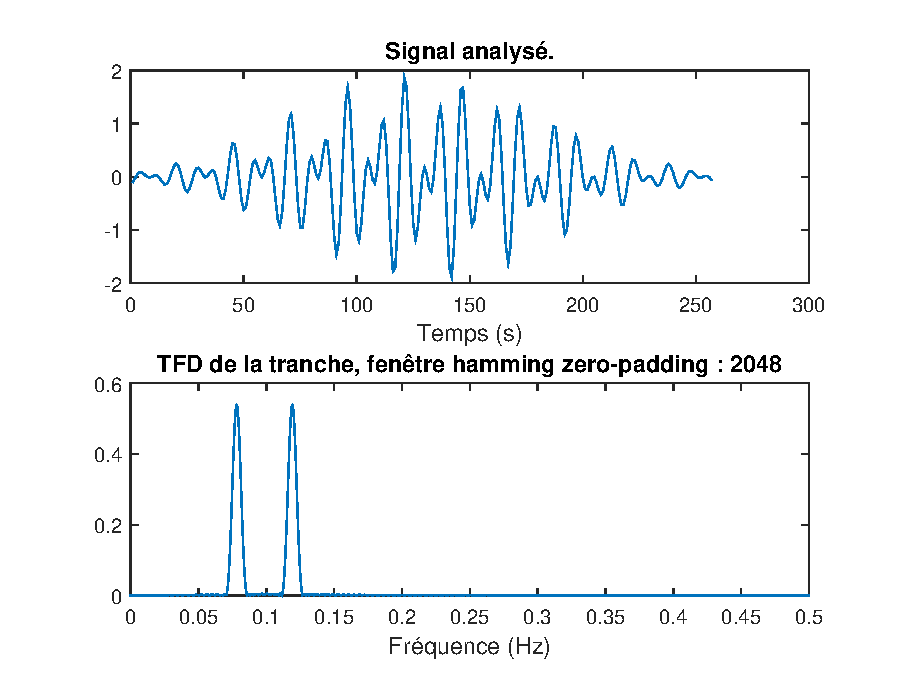
\includegraphics[width=\textwidth]{images/hamming.eps}
		% Title: glps_renderer figure
% Creator: GL2PS 1.3.8, (C) 1999-2012 C. Geuzaine
% For: Octave
% CreationDate: Wed Nov  8 10:42:42 2017
\begin{pgfpicture}
\pgfsetlinewidth{0.01pt}
\color[rgb]{1.000000,1.000000,1.000000}
\pgfpathmoveto{\pgfpoint{65.000015pt}{104.000000pt}}
\pgflineto{\pgfpoint{452.500031pt}{26.999981pt}}
\pgflineto{\pgfpoint{65.000015pt}{26.999981pt}}
\pgfpathclose
\pgfusepath{fill,stroke}
\pgfpathmoveto{\pgfpoint{65.000015pt}{104.000000pt}}
\pgflineto{\pgfpoint{452.500031pt}{104.000000pt}}
\pgflineto{\pgfpoint{452.500031pt}{26.999981pt}}
\pgfpathclose
\pgfusepath{fill,stroke}
\color[rgb]{0.000000,0.000000,0.000000}
\pgfsetlinewidth{0.500000pt}
\pgfsetdash{{16pt}{0pt}}{0pt}
\pgfpathmoveto{\pgfpoint{452.500031pt}{26.999981pt}}
\pgflineto{\pgfpoint{65.000015pt}{26.999981pt}}
\pgfusepath{stroke}
\pgfpathmoveto{\pgfpoint{452.500031pt}{104.000000pt}}
\pgflineto{\pgfpoint{65.000015pt}{104.000000pt}}
\pgfusepath{stroke}
\pgfpathmoveto{\pgfpoint{65.000015pt}{104.000000pt}}
\pgflineto{\pgfpoint{65.000015pt}{26.999981pt}}
\pgfusepath{stroke}
\pgfpathmoveto{\pgfpoint{452.500031pt}{104.000000pt}}
\pgflineto{\pgfpoint{452.500031pt}{26.999981pt}}
\pgfusepath{stroke}
\pgfsetdash{{0pt}{3pt}{1pt}{3pt}{1pt}{3pt}{1pt}{3pt}{1pt}{0pt}}{0pt}
\pgfpathmoveto{\pgfpoint{65.000015pt}{104.000000pt}}
\pgflineto{\pgfpoint{65.000015pt}{26.999981pt}}
\pgfusepath{stroke}
\pgfpathmoveto{\pgfpoint{142.500031pt}{104.000000pt}}
\pgflineto{\pgfpoint{142.500031pt}{26.999981pt}}
\pgfusepath{stroke}
\pgfpathmoveto{\pgfpoint{220.000031pt}{104.000000pt}}
\pgflineto{\pgfpoint{220.000031pt}{26.999981pt}}
\pgfusepath{stroke}
\pgfpathmoveto{\pgfpoint{297.500031pt}{104.000000pt}}
\pgflineto{\pgfpoint{297.500031pt}{26.999981pt}}
\pgfusepath{stroke}
\pgfpathmoveto{\pgfpoint{375.000061pt}{104.000000pt}}
\pgflineto{\pgfpoint{375.000061pt}{26.999981pt}}
\pgfusepath{stroke}
\pgfpathmoveto{\pgfpoint{452.500031pt}{104.000000pt}}
\pgflineto{\pgfpoint{452.500031pt}{26.999981pt}}
\pgfusepath{stroke}
\pgfsetdash{{16pt}{0pt}}{0pt}
\pgfpathmoveto{\pgfpoint{65.000015pt}{30.874983pt}}
\pgflineto{\pgfpoint{65.000015pt}{26.999981pt}}
\pgfusepath{stroke}
\pgfpathmoveto{\pgfpoint{65.000015pt}{100.125008pt}}
\pgflineto{\pgfpoint{65.000015pt}{104.000000pt}}
\pgfusepath{stroke}
\pgfpathmoveto{\pgfpoint{142.500031pt}{30.874983pt}}
\pgflineto{\pgfpoint{142.500031pt}{26.999981pt}}
\pgfusepath{stroke}
\pgfpathmoveto{\pgfpoint{142.500031pt}{100.125008pt}}
\pgflineto{\pgfpoint{142.500031pt}{104.000000pt}}
\pgfusepath{stroke}
\pgfpathmoveto{\pgfpoint{220.000031pt}{30.874983pt}}
\pgflineto{\pgfpoint{220.000031pt}{26.999981pt}}
\pgfusepath{stroke}
\pgfpathmoveto{\pgfpoint{220.000031pt}{100.125008pt}}
\pgflineto{\pgfpoint{220.000031pt}{104.000000pt}}
\pgfusepath{stroke}
\pgfpathmoveto{\pgfpoint{297.500031pt}{30.874983pt}}
\pgflineto{\pgfpoint{297.500031pt}{26.999981pt}}
\pgfusepath{stroke}
\pgfpathmoveto{\pgfpoint{297.500031pt}{100.125008pt}}
\pgflineto{\pgfpoint{297.500031pt}{104.000000pt}}
\pgfusepath{stroke}
\pgfpathmoveto{\pgfpoint{375.000061pt}{30.874983pt}}
\pgflineto{\pgfpoint{375.000061pt}{26.999981pt}}
\pgfusepath{stroke}
\pgfpathmoveto{\pgfpoint{375.000061pt}{100.125008pt}}
\pgflineto{\pgfpoint{375.000061pt}{104.000000pt}}
\pgfusepath{stroke}
\pgfpathmoveto{\pgfpoint{452.500031pt}{30.874983pt}}
\pgflineto{\pgfpoint{452.500031pt}{26.999981pt}}
\pgfusepath{stroke}
\pgfpathmoveto{\pgfpoint{452.500031pt}{100.125008pt}}
\pgflineto{\pgfpoint{452.500031pt}{104.000000pt}}
\pgfusepath{stroke}
{
\pgftransformshift{\pgfpoint{65.000015pt}{21.999977pt}}
\pgfnode{rectangle}{north}{\fontsize{10}{0}\selectfont\textcolor[rgb]{0,0,0}{{0}}}{}{\pgfusepath{discard}}}
{
\pgftransformshift{\pgfpoint{142.500015pt}{21.999977pt}}
\pgfnode{rectangle}{north}{\fontsize{10}{0}\selectfont\textcolor[rgb]{0,0,0}{{0.1}}}{}{\pgfusepath{discard}}}
{
\pgftransformshift{\pgfpoint{220.000015pt}{21.999977pt}}
\pgfnode{rectangle}{north}{\fontsize{10}{0}\selectfont\textcolor[rgb]{0,0,0}{{0.2}}}{}{\pgfusepath{discard}}}
{
\pgftransformshift{\pgfpoint{297.500031pt}{21.999977pt}}
\pgfnode{rectangle}{north}{\fontsize{10}{0}\selectfont\textcolor[rgb]{0,0,0}{{0.3}}}{}{\pgfusepath{discard}}}
{
\pgftransformshift{\pgfpoint{375.000031pt}{21.999977pt}}
\pgfnode{rectangle}{north}{\fontsize{10}{0}\selectfont\textcolor[rgb]{0,0,0}{{0.4}}}{}{\pgfusepath{discard}}}
{
\pgftransformshift{\pgfpoint{452.500031pt}{21.999977pt}}
\pgfnode{rectangle}{north}{\fontsize{10}{0}\selectfont\textcolor[rgb]{0,0,0}{{0.5}}}{}{\pgfusepath{discard}}}
\pgfsetdash{{0pt}{3pt}{1pt}{3pt}{1pt}{3pt}{1pt}{3pt}{1pt}{0pt}}{0pt}
\pgfpathmoveto{\pgfpoint{452.500031pt}{26.999981pt}}
\pgflineto{\pgfpoint{65.000015pt}{26.999981pt}}
\pgfusepath{stroke}
\pgfpathmoveto{\pgfpoint{452.500031pt}{37.999985pt}}
\pgflineto{\pgfpoint{65.000015pt}{37.999985pt}}
\pgfusepath{stroke}
\pgfpathmoveto{\pgfpoint{452.500031pt}{48.999989pt}}
\pgflineto{\pgfpoint{65.000015pt}{48.999989pt}}
\pgfusepath{stroke}
\pgfpathmoveto{\pgfpoint{452.500031pt}{59.999992pt}}
\pgflineto{\pgfpoint{65.000015pt}{59.999992pt}}
\pgfusepath{stroke}
\pgfpathmoveto{\pgfpoint{452.500031pt}{70.999992pt}}
\pgflineto{\pgfpoint{65.000015pt}{70.999992pt}}
\pgfusepath{stroke}
\pgfpathmoveto{\pgfpoint{452.500031pt}{82.000000pt}}
\pgflineto{\pgfpoint{65.000015pt}{82.000000pt}}
\pgfusepath{stroke}
\pgfpathmoveto{\pgfpoint{452.500031pt}{93.000000pt}}
\pgflineto{\pgfpoint{65.000015pt}{93.000000pt}}
\pgfusepath{stroke}
\pgfpathmoveto{\pgfpoint{452.500031pt}{104.000000pt}}
\pgflineto{\pgfpoint{65.000015pt}{104.000000pt}}
\pgfusepath{stroke}
\pgfsetdash{{16pt}{0pt}}{0pt}
\pgfpathmoveto{\pgfpoint{68.870026pt}{26.999981pt}}
\pgflineto{\pgfpoint{65.000015pt}{26.999981pt}}
\pgfusepath{stroke}
\pgfpathmoveto{\pgfpoint{448.630005pt}{26.999981pt}}
\pgflineto{\pgfpoint{452.500031pt}{26.999981pt}}
\pgfusepath{stroke}
\pgfpathmoveto{\pgfpoint{68.870026pt}{37.999985pt}}
\pgflineto{\pgfpoint{65.000015pt}{37.999985pt}}
\pgfusepath{stroke}
\pgfpathmoveto{\pgfpoint{448.630005pt}{37.999985pt}}
\pgflineto{\pgfpoint{452.500031pt}{37.999985pt}}
\pgfusepath{stroke}
\pgfpathmoveto{\pgfpoint{68.870026pt}{48.999989pt}}
\pgflineto{\pgfpoint{65.000015pt}{48.999989pt}}
\pgfusepath{stroke}
\pgfpathmoveto{\pgfpoint{448.630005pt}{48.999989pt}}
\pgflineto{\pgfpoint{452.500031pt}{48.999989pt}}
\pgfusepath{stroke}
\pgfpathmoveto{\pgfpoint{68.870026pt}{59.999992pt}}
\pgflineto{\pgfpoint{65.000015pt}{59.999992pt}}
\pgfusepath{stroke}
\pgfpathmoveto{\pgfpoint{448.630005pt}{59.999992pt}}
\pgflineto{\pgfpoint{452.500031pt}{59.999992pt}}
\pgfusepath{stroke}
\pgfpathmoveto{\pgfpoint{68.870026pt}{70.999992pt}}
\pgflineto{\pgfpoint{65.000015pt}{70.999992pt}}
\pgfusepath{stroke}
\pgfpathmoveto{\pgfpoint{448.630005pt}{70.999992pt}}
\pgflineto{\pgfpoint{452.500031pt}{70.999992pt}}
\pgfusepath{stroke}
\pgfpathmoveto{\pgfpoint{68.870026pt}{82.000000pt}}
\pgflineto{\pgfpoint{65.000015pt}{82.000000pt}}
\pgfusepath{stroke}
\pgfpathmoveto{\pgfpoint{448.630005pt}{82.000000pt}}
\pgflineto{\pgfpoint{452.500031pt}{82.000000pt}}
\pgfusepath{stroke}
\pgfpathmoveto{\pgfpoint{68.870026pt}{93.000000pt}}
\pgflineto{\pgfpoint{65.000015pt}{93.000000pt}}
\pgfusepath{stroke}
\pgfpathmoveto{\pgfpoint{448.630005pt}{93.000000pt}}
\pgflineto{\pgfpoint{452.500031pt}{93.000000pt}}
\pgfusepath{stroke}
\pgfpathmoveto{\pgfpoint{68.870026pt}{104.000000pt}}
\pgflineto{\pgfpoint{65.000015pt}{104.000000pt}}
\pgfusepath{stroke}
\pgfpathmoveto{\pgfpoint{448.630005pt}{104.000000pt}}
\pgflineto{\pgfpoint{452.500031pt}{104.000000pt}}
\pgfusepath{stroke}
{
\pgftransformshift{\pgfpoint{60.006454pt}{26.999981pt}}
\pgfnode{rectangle}{east}{\fontsize{10}{0}\selectfont\textcolor[rgb]{0,0,0}{{0}}}{}{\pgfusepath{discard}}}
{
\pgftransformshift{\pgfpoint{60.006454pt}{37.999985pt}}
\pgfnode{rectangle}{east}{\fontsize{10}{0}\selectfont\textcolor[rgb]{0,0,0}{{0.1}}}{}{\pgfusepath{discard}}}
{
\pgftransformshift{\pgfpoint{60.006454pt}{48.999989pt}}
\pgfnode{rectangle}{east}{\fontsize{10}{0}\selectfont\textcolor[rgb]{0,0,0}{{0.2}}}{}{\pgfusepath{discard}}}
{
\pgftransformshift{\pgfpoint{60.006454pt}{59.999992pt}}
\pgfnode{rectangle}{east}{\fontsize{10}{0}\selectfont\textcolor[rgb]{0,0,0}{{0.3}}}{}{\pgfusepath{discard}}}
{
\pgftransformshift{\pgfpoint{60.006454pt}{70.999992pt}}
\pgfnode{rectangle}{east}{\fontsize{10}{0}\selectfont\textcolor[rgb]{0,0,0}{{0.4}}}{}{\pgfusepath{discard}}}
{
\pgftransformshift{\pgfpoint{60.006454pt}{82.000000pt}}
\pgfnode{rectangle}{east}{\fontsize{10}{0}\selectfont\textcolor[rgb]{0,0,0}{{0.5}}}{}{\pgfusepath{discard}}}
{
\pgftransformshift{\pgfpoint{60.006454pt}{93.000000pt}}
\pgfnode{rectangle}{east}{\fontsize{10}{0}\selectfont\textcolor[rgb]{0,0,0}{{0.6}}}{}{\pgfusepath{discard}}}
{
\pgftransformshift{\pgfpoint{60.006454pt}{104.000000pt}}
\pgfnode{rectangle}{east}{\fontsize{10}{0}\selectfont\textcolor[rgb]{0,0,0}{{0.7}}}{}{\pgfusepath{discard}}}
{
\pgftransformshift{\pgfpoint{258.750031pt}{10.999977pt}}
\pgfnode{rectangle}{north}{\fontsize{10}{0}\selectfont\textcolor[rgb]{0,0,0}{{Fréquence (Hz)}}}{}{\pgfusepath{discard}}}
\color[rgb]{0.000000,0.000000,1.000000}
\pgfsetdash{}{0pt}
\pgfpathmoveto{\pgfpoint{65.189224pt}{27.101219pt}}
\pgflineto{\pgfpoint{65.000015pt}{27.102337pt}}
\pgfusepath{stroke}
\pgfpathmoveto{\pgfpoint{65.378433pt}{27.097946pt}}
\pgflineto{\pgfpoint{65.189224pt}{27.101219pt}}
\pgfusepath{stroke}
\pgfpathmoveto{\pgfpoint{65.567642pt}{27.092766pt}}
\pgflineto{\pgfpoint{65.378433pt}{27.097946pt}}
\pgfusepath{stroke}
\pgfpathmoveto{\pgfpoint{65.756836pt}{27.086094pt}}
\pgflineto{\pgfpoint{65.567642pt}{27.092766pt}}
\pgfusepath{stroke}
\pgfpathmoveto{\pgfpoint{65.946060pt}{27.078579pt}}
\pgflineto{\pgfpoint{65.756836pt}{27.086094pt}}
\pgfusepath{stroke}
\pgfpathmoveto{\pgfpoint{66.135269pt}{27.071129pt}}
\pgflineto{\pgfpoint{65.946060pt}{27.078579pt}}
\pgfusepath{stroke}
\pgfpathmoveto{\pgfpoint{66.324478pt}{27.064941pt}}
\pgflineto{\pgfpoint{66.135269pt}{27.071129pt}}
\pgfusepath{stroke}
\pgfpathmoveto{\pgfpoint{66.513687pt}{27.061359pt}}
\pgflineto{\pgfpoint{66.324478pt}{27.064941pt}}
\pgfusepath{stroke}
\pgfpathmoveto{\pgfpoint{66.702881pt}{27.061359pt}}
\pgflineto{\pgfpoint{66.513687pt}{27.061359pt}}
\pgfusepath{stroke}
\pgfpathmoveto{\pgfpoint{66.892105pt}{27.064980pt}}
\pgflineto{\pgfpoint{66.702881pt}{27.061359pt}}
\pgfusepath{stroke}
\pgfpathmoveto{\pgfpoint{67.081314pt}{27.071270pt}}
\pgflineto{\pgfpoint{66.892105pt}{27.064980pt}}
\pgfusepath{stroke}
\pgfpathmoveto{\pgfpoint{67.270523pt}{27.078899pt}}
\pgflineto{\pgfpoint{67.081314pt}{27.071270pt}}
\pgfusepath{stroke}
\pgfpathmoveto{\pgfpoint{67.459732pt}{27.086655pt}}
\pgflineto{\pgfpoint{67.270523pt}{27.078899pt}}
\pgfusepath{stroke}
\pgfpathmoveto{\pgfpoint{67.648926pt}{27.093590pt}}
\pgflineto{\pgfpoint{67.459732pt}{27.086655pt}}
\pgfusepath{stroke}
\pgfpathmoveto{\pgfpoint{67.838150pt}{27.099037pt}}
\pgflineto{\pgfpoint{67.648926pt}{27.093590pt}}
\pgfusepath{stroke}
\pgfpathmoveto{\pgfpoint{68.027359pt}{27.102531pt}}
\pgflineto{\pgfpoint{67.838150pt}{27.099037pt}}
\pgfusepath{stroke}
\pgfpathmoveto{\pgfpoint{68.216568pt}{27.103806pt}}
\pgflineto{\pgfpoint{68.027359pt}{27.102531pt}}
\pgfusepath{stroke}
\pgfpathmoveto{\pgfpoint{68.405777pt}{27.102745pt}}
\pgflineto{\pgfpoint{68.216568pt}{27.103806pt}}
\pgfusepath{stroke}
\pgfpathmoveto{\pgfpoint{68.594971pt}{27.099415pt}}
\pgflineto{\pgfpoint{68.405777pt}{27.102745pt}}
\pgfusepath{stroke}
\pgfpathmoveto{\pgfpoint{68.784195pt}{27.094032pt}}
\pgflineto{\pgfpoint{68.594971pt}{27.099415pt}}
\pgfusepath{stroke}
\pgfpathmoveto{\pgfpoint{68.973404pt}{27.087029pt}}
\pgflineto{\pgfpoint{68.784195pt}{27.094032pt}}
\pgfusepath{stroke}
\pgfpathmoveto{\pgfpoint{69.162613pt}{27.079060pt}}
\pgflineto{\pgfpoint{68.973404pt}{27.087029pt}}
\pgfusepath{stroke}
\pgfpathmoveto{\pgfpoint{69.351822pt}{27.071098pt}}
\pgflineto{\pgfpoint{69.162613pt}{27.079060pt}}
\pgfusepath{stroke}
\pgfpathmoveto{\pgfpoint{69.541016pt}{27.064472pt}}
\pgflineto{\pgfpoint{69.351822pt}{27.071098pt}}
\pgfusepath{stroke}
\pgfpathmoveto{\pgfpoint{69.730240pt}{27.060719pt}}
\pgflineto{\pgfpoint{69.541016pt}{27.064472pt}}
\pgfusepath{stroke}
\pgfpathmoveto{\pgfpoint{69.919449pt}{27.060986pt}}
\pgflineto{\pgfpoint{69.730240pt}{27.060719pt}}
\pgfusepath{stroke}
\pgfpathmoveto{\pgfpoint{70.108658pt}{27.065289pt}}
\pgflineto{\pgfpoint{69.919449pt}{27.060986pt}}
\pgfusepath{stroke}
\pgfpathmoveto{\pgfpoint{70.297867pt}{27.072487pt}}
\pgflineto{\pgfpoint{70.108658pt}{27.065289pt}}
\pgfusepath{stroke}
\pgfpathmoveto{\pgfpoint{70.487061pt}{27.081043pt}}
\pgflineto{\pgfpoint{70.297867pt}{27.072487pt}}
\pgfusepath{stroke}
\pgfpathmoveto{\pgfpoint{70.676285pt}{27.089630pt}}
\pgflineto{\pgfpoint{70.487061pt}{27.081043pt}}
\pgfusepath{stroke}
\pgfpathmoveto{\pgfpoint{70.865494pt}{27.097229pt}}
\pgflineto{\pgfpoint{70.676285pt}{27.089630pt}}
\pgfusepath{stroke}
\pgfpathmoveto{\pgfpoint{71.054703pt}{27.103123pt}}
\pgflineto{\pgfpoint{70.865494pt}{27.097229pt}}
\pgfusepath{stroke}
\pgfpathmoveto{\pgfpoint{71.243912pt}{27.106823pt}}
\pgflineto{\pgfpoint{71.054703pt}{27.103123pt}}
\pgfusepath{stroke}
\pgfpathmoveto{\pgfpoint{71.433105pt}{27.108040pt}}
\pgflineto{\pgfpoint{71.243912pt}{27.106823pt}}
\pgfusepath{stroke}
\pgfpathmoveto{\pgfpoint{71.622330pt}{27.106655pt}}
\pgflineto{\pgfpoint{71.433105pt}{27.108040pt}}
\pgfusepath{stroke}
\pgfpathmoveto{\pgfpoint{71.811539pt}{27.102730pt}}
\pgflineto{\pgfpoint{71.622330pt}{27.106655pt}}
\pgfusepath{stroke}
\pgfpathmoveto{\pgfpoint{72.000748pt}{27.096523pt}}
\pgflineto{\pgfpoint{71.811539pt}{27.102730pt}}
\pgfusepath{stroke}
\pgfpathmoveto{\pgfpoint{72.189957pt}{27.088501pt}}
\pgflineto{\pgfpoint{72.000748pt}{27.096523pt}}
\pgfusepath{stroke}
\pgfpathmoveto{\pgfpoint{72.379150pt}{27.079422pt}}
\pgflineto{\pgfpoint{72.189957pt}{27.088501pt}}
\pgfusepath{stroke}
\pgfpathmoveto{\pgfpoint{72.568375pt}{27.070442pt}}
\pgflineto{\pgfpoint{72.379150pt}{27.079422pt}}
\pgfusepath{stroke}
\pgfpathmoveto{\pgfpoint{72.757584pt}{27.063187pt}}
\pgflineto{\pgfpoint{72.568375pt}{27.070442pt}}
\pgfusepath{stroke}
\pgfpathmoveto{\pgfpoint{72.946793pt}{27.059578pt}}
\pgflineto{\pgfpoint{72.757584pt}{27.063187pt}}
\pgfusepath{stroke}
\pgfpathmoveto{\pgfpoint{73.136002pt}{27.060936pt}}
\pgflineto{\pgfpoint{72.946793pt}{27.059578pt}}
\pgfusepath{stroke}
\pgfpathmoveto{\pgfpoint{73.325195pt}{27.066944pt}}
\pgflineto{\pgfpoint{73.136002pt}{27.060936pt}}
\pgfusepath{stroke}
\pgfpathmoveto{\pgfpoint{73.514420pt}{27.075924pt}}
\pgflineto{\pgfpoint{73.325195pt}{27.066944pt}}
\pgfusepath{stroke}
\pgfpathmoveto{\pgfpoint{73.703629pt}{27.086025pt}}
\pgflineto{\pgfpoint{73.514420pt}{27.075924pt}}
\pgfusepath{stroke}
\pgfpathmoveto{\pgfpoint{73.892838pt}{27.095772pt}}
\pgflineto{\pgfpoint{73.703629pt}{27.086025pt}}
\pgfusepath{stroke}
\pgfpathmoveto{\pgfpoint{74.082047pt}{27.104115pt}}
\pgflineto{\pgfpoint{73.892838pt}{27.095772pt}}
\pgfusepath{stroke}
\pgfpathmoveto{\pgfpoint{74.271240pt}{27.110313pt}}
\pgflineto{\pgfpoint{74.082047pt}{27.104115pt}}
\pgfusepath{stroke}
\pgfpathmoveto{\pgfpoint{74.460464pt}{27.113888pt}}
\pgflineto{\pgfpoint{74.271240pt}{27.110313pt}}
\pgfusepath{stroke}
\pgfpathmoveto{\pgfpoint{74.649673pt}{27.114563pt}}
\pgflineto{\pgfpoint{74.460464pt}{27.113888pt}}
\pgfusepath{stroke}
\pgfpathmoveto{\pgfpoint{74.838882pt}{27.112247pt}}
\pgflineto{\pgfpoint{74.649673pt}{27.114563pt}}
\pgfusepath{stroke}
\pgfpathmoveto{\pgfpoint{75.028091pt}{27.107056pt}}
\pgflineto{\pgfpoint{74.838882pt}{27.112247pt}}
\pgfusepath{stroke}
\pgfpathmoveto{\pgfpoint{75.217285pt}{27.099312pt}}
\pgflineto{\pgfpoint{75.028091pt}{27.107056pt}}
\pgfusepath{stroke}
\pgfpathmoveto{\pgfpoint{75.406509pt}{27.089603pt}}
\pgflineto{\pgfpoint{75.217285pt}{27.099312pt}}
\pgfusepath{stroke}
\pgfpathmoveto{\pgfpoint{75.595718pt}{27.078884pt}}
\pgflineto{\pgfpoint{75.406509pt}{27.089603pt}}
\pgfusepath{stroke}
\pgfpathmoveto{\pgfpoint{75.784927pt}{27.068649pt}}
\pgflineto{\pgfpoint{75.595718pt}{27.078884pt}}
\pgfusepath{stroke}
\pgfpathmoveto{\pgfpoint{75.974136pt}{27.061066pt}}
\pgflineto{\pgfpoint{75.784927pt}{27.068649pt}}
\pgfusepath{stroke}
\pgfpathmoveto{\pgfpoint{76.163330pt}{27.058613pt}}
\pgflineto{\pgfpoint{75.974136pt}{27.061066pt}}
\pgfusepath{stroke}
\pgfpathmoveto{\pgfpoint{76.352554pt}{27.062450pt}}
\pgflineto{\pgfpoint{76.163330pt}{27.058613pt}}
\pgfusepath{stroke}
\pgfpathmoveto{\pgfpoint{76.541763pt}{27.071308pt}}
\pgflineto{\pgfpoint{76.352554pt}{27.062450pt}}
\pgfusepath{stroke}
\pgfpathmoveto{\pgfpoint{76.730972pt}{27.082752pt}}
\pgflineto{\pgfpoint{76.541763pt}{27.071308pt}}
\pgfusepath{stroke}
\pgfpathmoveto{\pgfpoint{76.920181pt}{27.094654pt}}
\pgflineto{\pgfpoint{76.730972pt}{27.082752pt}}
\pgfusepath{stroke}
\pgfpathmoveto{\pgfpoint{77.109375pt}{27.105518pt}}
\pgflineto{\pgfpoint{76.920181pt}{27.094654pt}}
\pgfusepath{stroke}
\pgfpathmoveto{\pgfpoint{77.298599pt}{27.114319pt}}
\pgflineto{\pgfpoint{77.109375pt}{27.105518pt}}
\pgfusepath{stroke}
\pgfpathmoveto{\pgfpoint{77.487808pt}{27.120369pt}}
\pgflineto{\pgfpoint{77.298599pt}{27.114319pt}}
\pgfusepath{stroke}
\pgfpathmoveto{\pgfpoint{77.677017pt}{27.123230pt}}
\pgflineto{\pgfpoint{77.487808pt}{27.120369pt}}
\pgfusepath{stroke}
\pgfpathmoveto{\pgfpoint{77.866226pt}{27.122677pt}}
\pgflineto{\pgfpoint{77.677017pt}{27.123230pt}}
\pgfusepath{stroke}
\pgfpathmoveto{\pgfpoint{78.055420pt}{27.118683pt}}
\pgflineto{\pgfpoint{77.866226pt}{27.122677pt}}
\pgfusepath{stroke}
\pgfpathmoveto{\pgfpoint{78.244644pt}{27.111462pt}}
\pgflineto{\pgfpoint{78.055420pt}{27.118683pt}}
\pgfusepath{stroke}
\pgfpathmoveto{\pgfpoint{78.433853pt}{27.101471pt}}
\pgflineto{\pgfpoint{78.244644pt}{27.111462pt}}
\pgfusepath{stroke}
\pgfpathmoveto{\pgfpoint{78.623062pt}{27.089500pt}}
\pgflineto{\pgfpoint{78.433853pt}{27.101471pt}}
\pgfusepath{stroke}
\pgfpathmoveto{\pgfpoint{78.812271pt}{27.076820pt}}
\pgflineto{\pgfpoint{78.623062pt}{27.089500pt}}
\pgfusepath{stroke}
\pgfpathmoveto{\pgfpoint{79.001465pt}{27.065529pt}}
\pgflineto{\pgfpoint{78.812271pt}{27.076820pt}}
\pgfusepath{stroke}
\pgfpathmoveto{\pgfpoint{79.190689pt}{27.058708pt}}
\pgflineto{\pgfpoint{79.001465pt}{27.065529pt}}
\pgfusepath{stroke}
\pgfpathmoveto{\pgfpoint{79.379898pt}{27.059280pt}}
\pgflineto{\pgfpoint{79.190689pt}{27.058708pt}}
\pgfusepath{stroke}
\pgfpathmoveto{\pgfpoint{79.569107pt}{27.067257pt}}
\pgflineto{\pgfpoint{79.379898pt}{27.059280pt}}
\pgfusepath{stroke}
\pgfpathmoveto{\pgfpoint{79.758316pt}{27.079784pt}}
\pgflineto{\pgfpoint{79.569107pt}{27.067257pt}}
\pgfusepath{stroke}
\pgfpathmoveto{\pgfpoint{79.947510pt}{27.093849pt}}
\pgflineto{\pgfpoint{79.758316pt}{27.079784pt}}
\pgfusepath{stroke}
\pgfpathmoveto{\pgfpoint{80.136734pt}{27.107349pt}}
\pgflineto{\pgfpoint{79.947510pt}{27.093849pt}}
\pgfusepath{stroke}
\pgfpathmoveto{\pgfpoint{80.325943pt}{27.118904pt}}
\pgflineto{\pgfpoint{80.136734pt}{27.107349pt}}
\pgfusepath{stroke}
\pgfpathmoveto{\pgfpoint{80.515152pt}{27.127583pt}}
\pgflineto{\pgfpoint{80.325943pt}{27.118904pt}}
\pgfusepath{stroke}
\pgfpathmoveto{\pgfpoint{80.704361pt}{27.132786pt}}
\pgflineto{\pgfpoint{80.515152pt}{27.127583pt}}
\pgfusepath{stroke}
\pgfpathmoveto{\pgfpoint{80.893570pt}{27.134148pt}}
\pgflineto{\pgfpoint{80.704361pt}{27.132786pt}}
\pgfusepath{stroke}
\pgfpathmoveto{\pgfpoint{81.082779pt}{27.131531pt}}
\pgflineto{\pgfpoint{80.893570pt}{27.134148pt}}
\pgfusepath{stroke}
\pgfpathmoveto{\pgfpoint{81.271988pt}{27.125034pt}}
\pgflineto{\pgfpoint{81.082779pt}{27.131531pt}}
\pgfusepath{stroke}
\pgfpathmoveto{\pgfpoint{81.461197pt}{27.115005pt}}
\pgflineto{\pgfpoint{81.271988pt}{27.125034pt}}
\pgfusepath{stroke}
\pgfpathmoveto{\pgfpoint{81.650406pt}{27.102104pt}}
\pgflineto{\pgfpoint{81.461197pt}{27.115005pt}}
\pgfusepath{stroke}
\pgfpathmoveto{\pgfpoint{81.839615pt}{27.087437pt}}
\pgflineto{\pgfpoint{81.650406pt}{27.102104pt}}
\pgfusepath{stroke}
\pgfpathmoveto{\pgfpoint{82.028824pt}{27.072857pt}}
\pgflineto{\pgfpoint{81.839615pt}{27.087437pt}}
\pgfusepath{stroke}
\pgfpathmoveto{\pgfpoint{82.218033pt}{27.061527pt}}
\pgflineto{\pgfpoint{82.028824pt}{27.072857pt}}
\pgfusepath{stroke}
\pgfpathmoveto{\pgfpoint{82.407242pt}{27.057777pt}}
\pgflineto{\pgfpoint{82.218033pt}{27.061527pt}}
\pgfusepath{stroke}
\pgfpathmoveto{\pgfpoint{82.596451pt}{27.063858pt}}
\pgflineto{\pgfpoint{82.407242pt}{27.057777pt}}
\pgfusepath{stroke}
\pgfpathmoveto{\pgfpoint{82.785660pt}{27.077110pt}}
\pgflineto{\pgfpoint{82.596451pt}{27.063858pt}}
\pgfusepath{stroke}
\pgfpathmoveto{\pgfpoint{82.974869pt}{27.093349pt}}
\pgflineto{\pgfpoint{82.785660pt}{27.077110pt}}
\pgfusepath{stroke}
\pgfpathmoveto{\pgfpoint{83.164078pt}{27.109634pt}}
\pgflineto{\pgfpoint{82.974869pt}{27.093349pt}}
\pgfusepath{stroke}
\pgfpathmoveto{\pgfpoint{83.353287pt}{27.124126pt}}
\pgflineto{\pgfpoint{83.164078pt}{27.109634pt}}
\pgfusepath{stroke}
\pgfpathmoveto{\pgfpoint{83.542496pt}{27.135635pt}}
\pgflineto{\pgfpoint{83.353287pt}{27.124126pt}}
\pgfusepath{stroke}
\pgfpathmoveto{\pgfpoint{83.731705pt}{27.143379pt}}
\pgflineto{\pgfpoint{83.542496pt}{27.135635pt}}
\pgfusepath{stroke}
\pgfpathmoveto{\pgfpoint{83.920914pt}{27.146839pt}}
\pgflineto{\pgfpoint{83.731705pt}{27.143379pt}}
\pgfusepath{stroke}
\pgfpathmoveto{\pgfpoint{84.110123pt}{27.145775pt}}
\pgflineto{\pgfpoint{83.920914pt}{27.146839pt}}
\pgfusepath{stroke}
\pgfpathmoveto{\pgfpoint{84.299332pt}{27.140179pt}}
\pgflineto{\pgfpoint{84.110123pt}{27.145775pt}}
\pgfusepath{stroke}
\pgfpathmoveto{\pgfpoint{84.488541pt}{27.130299pt}}
\pgflineto{\pgfpoint{84.299332pt}{27.140179pt}}
\pgfusepath{stroke}
\pgfpathmoveto{\pgfpoint{84.677750pt}{27.116699pt}}
\pgflineto{\pgfpoint{84.488541pt}{27.130299pt}}
\pgfusepath{stroke}
\pgfpathmoveto{\pgfpoint{84.866959pt}{27.100342pt}}
\pgflineto{\pgfpoint{84.677750pt}{27.116699pt}}
\pgfusepath{stroke}
\pgfpathmoveto{\pgfpoint{85.056168pt}{27.082859pt}}
\pgflineto{\pgfpoint{84.866959pt}{27.100342pt}}
\pgfusepath{stroke}
\pgfpathmoveto{\pgfpoint{85.245377pt}{27.067184pt}}
\pgflineto{\pgfpoint{85.056168pt}{27.082859pt}}
\pgfusepath{stroke}
\pgfpathmoveto{\pgfpoint{85.434586pt}{27.058346pt}}
\pgflineto{\pgfpoint{85.245377pt}{27.067184pt}}
\pgfusepath{stroke}
\pgfpathmoveto{\pgfpoint{85.623795pt}{27.061295pt}}
\pgflineto{\pgfpoint{85.434586pt}{27.058346pt}}
\pgfusepath{stroke}
\pgfpathmoveto{\pgfpoint{85.813004pt}{27.074722pt}}
\pgflineto{\pgfpoint{85.623795pt}{27.061295pt}}
\pgfusepath{stroke}
\pgfpathmoveto{\pgfpoint{86.002213pt}{27.093143pt}}
\pgflineto{\pgfpoint{85.813004pt}{27.074722pt}}
\pgfusepath{stroke}
\pgfpathmoveto{\pgfpoint{86.191422pt}{27.112404pt}}
\pgflineto{\pgfpoint{86.002213pt}{27.093143pt}}
\pgfusepath{stroke}
\pgfpathmoveto{\pgfpoint{86.380630pt}{27.130074pt}}
\pgflineto{\pgfpoint{86.191422pt}{27.112404pt}}
\pgfusepath{stroke}
\pgfpathmoveto{\pgfpoint{86.569839pt}{27.144669pt}}
\pgflineto{\pgfpoint{86.380630pt}{27.130074pt}}
\pgfusepath{stroke}
\pgfpathmoveto{\pgfpoint{86.759048pt}{27.155186pt}}
\pgflineto{\pgfpoint{86.569839pt}{27.144669pt}}
\pgfusepath{stroke}
\pgfpathmoveto{\pgfpoint{86.948257pt}{27.160976pt}}
\pgflineto{\pgfpoint{86.759048pt}{27.155186pt}}
\pgfusepath{stroke}
\pgfpathmoveto{\pgfpoint{87.137466pt}{27.161663pt}}
\pgflineto{\pgfpoint{86.948257pt}{27.160976pt}}
\pgfusepath{stroke}
\pgfpathmoveto{\pgfpoint{87.326675pt}{27.157131pt}}
\pgflineto{\pgfpoint{87.137466pt}{27.161663pt}}
\pgfusepath{stroke}
\pgfpathmoveto{\pgfpoint{87.515884pt}{27.147556pt}}
\pgflineto{\pgfpoint{87.326675pt}{27.157131pt}}
\pgfusepath{stroke}
\pgfpathmoveto{\pgfpoint{87.705093pt}{27.133411pt}}
\pgflineto{\pgfpoint{87.515884pt}{27.147556pt}}
\pgfusepath{stroke}
\pgfpathmoveto{\pgfpoint{87.894302pt}{27.115559pt}}
\pgflineto{\pgfpoint{87.705093pt}{27.133411pt}}
\pgfusepath{stroke}
\pgfpathmoveto{\pgfpoint{88.083511pt}{27.095436pt}}
\pgflineto{\pgfpoint{87.894302pt}{27.115559pt}}
\pgfusepath{stroke}
\pgfpathmoveto{\pgfpoint{88.272720pt}{27.075676pt}}
\pgflineto{\pgfpoint{88.083511pt}{27.095436pt}}
\pgfusepath{stroke}
\pgfpathmoveto{\pgfpoint{88.461929pt}{27.061348pt}}
\pgflineto{\pgfpoint{88.272720pt}{27.075676pt}}
\pgfusepath{stroke}
\pgfpathmoveto{\pgfpoint{88.651138pt}{27.059811pt}}
\pgflineto{\pgfpoint{88.461929pt}{27.061348pt}}
\pgfusepath{stroke}
\pgfpathmoveto{\pgfpoint{88.840347pt}{27.072632pt}}
\pgflineto{\pgfpoint{88.651138pt}{27.059811pt}}
\pgfusepath{stroke}
\pgfpathmoveto{\pgfpoint{89.029556pt}{27.093204pt}}
\pgflineto{\pgfpoint{88.840347pt}{27.072632pt}}
\pgfusepath{stroke}
\pgfpathmoveto{\pgfpoint{89.218765pt}{27.115685pt}}
\pgflineto{\pgfpoint{89.029556pt}{27.093204pt}}
\pgfusepath{stroke}
\pgfpathmoveto{\pgfpoint{89.407974pt}{27.136860pt}}
\pgflineto{\pgfpoint{89.218765pt}{27.115685pt}}
\pgfusepath{stroke}
\pgfpathmoveto{\pgfpoint{89.597183pt}{27.154854pt}}
\pgflineto{\pgfpoint{89.407974pt}{27.136860pt}}
\pgfusepath{stroke}
\pgfpathmoveto{\pgfpoint{89.786392pt}{27.168457pt}}
\pgflineto{\pgfpoint{89.597183pt}{27.154854pt}}
\pgfusepath{stroke}
\pgfpathmoveto{\pgfpoint{89.975601pt}{27.176842pt}}
\pgflineto{\pgfpoint{89.786392pt}{27.168457pt}}
\pgfusepath{stroke}
\pgfpathmoveto{\pgfpoint{90.164810pt}{27.179501pt}}
\pgflineto{\pgfpoint{89.975601pt}{27.176842pt}}
\pgfusepath{stroke}
\pgfpathmoveto{\pgfpoint{90.354019pt}{27.176228pt}}
\pgflineto{\pgfpoint{90.164810pt}{27.179501pt}}
\pgfusepath{stroke}
\pgfpathmoveto{\pgfpoint{90.543228pt}{27.167099pt}}
\pgflineto{\pgfpoint{90.354019pt}{27.176228pt}}
\pgfusepath{stroke}
\pgfpathmoveto{\pgfpoint{90.732437pt}{27.152515pt}}
\pgflineto{\pgfpoint{90.543228pt}{27.167099pt}}
\pgfusepath{stroke}
\pgfpathmoveto{\pgfpoint{90.921646pt}{27.133251pt}}
\pgflineto{\pgfpoint{90.732437pt}{27.152515pt}}
\pgfusepath{stroke}
\pgfpathmoveto{\pgfpoint{91.110855pt}{27.110634pt}}
\pgflineto{\pgfpoint{90.921646pt}{27.133251pt}}
\pgfusepath{stroke}
\pgfpathmoveto{\pgfpoint{91.300064pt}{27.086994pt}}
\pgflineto{\pgfpoint{91.110855pt}{27.110634pt}}
\pgfusepath{stroke}
\pgfpathmoveto{\pgfpoint{91.489273pt}{27.067070pt}}
\pgflineto{\pgfpoint{91.300064pt}{27.086994pt}}
\pgfusepath{stroke}
\pgfpathmoveto{\pgfpoint{91.678482pt}{27.059761pt}}
\pgflineto{\pgfpoint{91.489273pt}{27.067070pt}}
\pgfusepath{stroke}
\pgfpathmoveto{\pgfpoint{91.867691pt}{27.070885pt}}
\pgflineto{\pgfpoint{91.678482pt}{27.059761pt}}
\pgfusepath{stroke}
\pgfpathmoveto{\pgfpoint{92.056900pt}{27.093529pt}}
\pgflineto{\pgfpoint{91.867691pt}{27.070885pt}}
\pgfusepath{stroke}
\pgfpathmoveto{\pgfpoint{92.246109pt}{27.119534pt}}
\pgflineto{\pgfpoint{92.056900pt}{27.093529pt}}
\pgfusepath{stroke}
\pgfpathmoveto{\pgfpoint{92.435318pt}{27.144600pt}}
\pgflineto{\pgfpoint{92.246109pt}{27.119534pt}}
\pgfusepath{stroke}
\pgfpathmoveto{\pgfpoint{92.624527pt}{27.166405pt}}
\pgflineto{\pgfpoint{92.435318pt}{27.144600pt}}
\pgfusepath{stroke}
\pgfpathmoveto{\pgfpoint{92.813736pt}{27.183464pt}}
\pgflineto{\pgfpoint{92.624527pt}{27.166405pt}}
\pgfusepath{stroke}
\pgfpathmoveto{\pgfpoint{93.002945pt}{27.194786pt}}
\pgflineto{\pgfpoint{92.813736pt}{27.183464pt}}
\pgfusepath{stroke}
\pgfpathmoveto{\pgfpoint{93.192154pt}{27.199707pt}}
\pgflineto{\pgfpoint{93.002945pt}{27.194786pt}}
\pgfusepath{stroke}
\pgfpathmoveto{\pgfpoint{93.381363pt}{27.197903pt}}
\pgflineto{\pgfpoint{93.192154pt}{27.199707pt}}
\pgfusepath{stroke}
\pgfpathmoveto{\pgfpoint{93.570572pt}{27.189358pt}}
\pgflineto{\pgfpoint{93.381363pt}{27.197903pt}}
\pgfusepath{stroke}
\pgfpathmoveto{\pgfpoint{93.759781pt}{27.174408pt}}
\pgflineto{\pgfpoint{93.570572pt}{27.189358pt}}
\pgfusepath{stroke}
\pgfpathmoveto{\pgfpoint{93.948990pt}{27.153770pt}}
\pgflineto{\pgfpoint{93.759781pt}{27.174408pt}}
\pgfusepath{stroke}
\pgfpathmoveto{\pgfpoint{94.138199pt}{27.128666pt}}
\pgflineto{\pgfpoint{93.948990pt}{27.153770pt}}
\pgfusepath{stroke}
\pgfpathmoveto{\pgfpoint{94.327408pt}{27.101223pt}}
\pgflineto{\pgfpoint{94.138199pt}{27.128666pt}}
\pgfusepath{stroke}
\pgfpathmoveto{\pgfpoint{94.516617pt}{27.075710pt}}
\pgflineto{\pgfpoint{94.327408pt}{27.101223pt}}
\pgfusepath{stroke}
\pgfpathmoveto{\pgfpoint{94.705826pt}{27.061573pt}}
\pgflineto{\pgfpoint{94.516617pt}{27.075710pt}}
\pgfusepath{stroke}
\pgfpathmoveto{\pgfpoint{94.895035pt}{27.069557pt}}
\pgflineto{\pgfpoint{94.705826pt}{27.061573pt}}
\pgfusepath{stroke}
\pgfpathmoveto{\pgfpoint{95.084244pt}{27.094097pt}}
\pgflineto{\pgfpoint{94.895035pt}{27.069557pt}}
\pgfusepath{stroke}
\pgfpathmoveto{\pgfpoint{95.273453pt}{27.124001pt}}
\pgflineto{\pgfpoint{95.084244pt}{27.094097pt}}
\pgfusepath{stroke}
\pgfpathmoveto{\pgfpoint{95.462662pt}{27.153454pt}}
\pgflineto{\pgfpoint{95.273453pt}{27.124001pt}}
\pgfusepath{stroke}
\pgfpathmoveto{\pgfpoint{95.651871pt}{27.179573pt}}
\pgflineto{\pgfpoint{95.462662pt}{27.153454pt}}
\pgfusepath{stroke}
\pgfpathmoveto{\pgfpoint{95.841080pt}{27.200577pt}}
\pgflineto{\pgfpoint{95.651871pt}{27.179573pt}}
\pgfusepath{stroke}
\pgfpathmoveto{\pgfpoint{96.030289pt}{27.215244pt}}
\pgflineto{\pgfpoint{95.841080pt}{27.200577pt}}
\pgfusepath{stroke}
\pgfpathmoveto{\pgfpoint{96.219498pt}{27.222767pt}}
\pgflineto{\pgfpoint{96.030289pt}{27.215244pt}}
\pgfusepath{stroke}
\pgfpathmoveto{\pgfpoint{96.408707pt}{27.222687pt}}
\pgflineto{\pgfpoint{96.219498pt}{27.222767pt}}
\pgfusepath{stroke}
\pgfpathmoveto{\pgfpoint{96.597916pt}{27.214886pt}}
\pgflineto{\pgfpoint{96.408707pt}{27.222687pt}}
\pgfusepath{stroke}
\pgfpathmoveto{\pgfpoint{96.787125pt}{27.199635pt}}
\pgflineto{\pgfpoint{96.597916pt}{27.214886pt}}
\pgfusepath{stroke}
\pgfpathmoveto{\pgfpoint{96.976334pt}{27.177586pt}}
\pgflineto{\pgfpoint{96.787125pt}{27.199635pt}}
\pgfusepath{stroke}
\pgfpathmoveto{\pgfpoint{97.165543pt}{27.149918pt}}
\pgflineto{\pgfpoint{96.976334pt}{27.177586pt}}
\pgfusepath{stroke}
\pgfpathmoveto{\pgfpoint{97.354752pt}{27.118595pt}}
\pgflineto{\pgfpoint{97.165543pt}{27.149918pt}}
\pgfusepath{stroke}
\pgfpathmoveto{\pgfpoint{97.543961pt}{27.087467pt}}
\pgflineto{\pgfpoint{97.354752pt}{27.118595pt}}
\pgfusepath{stroke}
\pgfpathmoveto{\pgfpoint{97.733170pt}{27.065735pt}}
\pgflineto{\pgfpoint{97.543961pt}{27.087467pt}}
\pgfusepath{stroke}
\pgfpathmoveto{\pgfpoint{97.922379pt}{27.068806pt}}
\pgflineto{\pgfpoint{97.733170pt}{27.065735pt}}
\pgfusepath{stroke}
\pgfpathmoveto{\pgfpoint{98.111588pt}{27.094906pt}}
\pgflineto{\pgfpoint{97.922379pt}{27.068806pt}}
\pgfusepath{stroke}
\pgfpathmoveto{\pgfpoint{98.300797pt}{27.129150pt}}
\pgflineto{\pgfpoint{98.111588pt}{27.094906pt}}
\pgfusepath{stroke}
\pgfpathmoveto{\pgfpoint{98.490005pt}{27.163612pt}}
\pgflineto{\pgfpoint{98.300797pt}{27.129150pt}}
\pgfusepath{stroke}
\pgfpathmoveto{\pgfpoint{98.679214pt}{27.194672pt}}
\pgflineto{\pgfpoint{98.490005pt}{27.163612pt}}
\pgfusepath{stroke}
\pgfpathmoveto{\pgfpoint{98.868423pt}{27.220192pt}}
\pgflineto{\pgfpoint{98.679214pt}{27.194672pt}}
\pgfusepath{stroke}
\pgfpathmoveto{\pgfpoint{99.057632pt}{27.238728pt}}
\pgflineto{\pgfpoint{98.868423pt}{27.220192pt}}
\pgfusepath{stroke}
\pgfpathmoveto{\pgfpoint{99.246841pt}{27.249268pt}}
\pgflineto{\pgfpoint{99.057632pt}{27.238728pt}}
\pgfusepath{stroke}
\pgfpathmoveto{\pgfpoint{99.436050pt}{27.251205pt}}
\pgflineto{\pgfpoint{99.246841pt}{27.249268pt}}
\pgfusepath{stroke}
\pgfpathmoveto{\pgfpoint{99.625259pt}{27.244331pt}}
\pgflineto{\pgfpoint{99.436050pt}{27.251205pt}}
\pgfusepath{stroke}
\pgfpathmoveto{\pgfpoint{99.814468pt}{27.228813pt}}
\pgflineto{\pgfpoint{99.625259pt}{27.244331pt}}
\pgfusepath{stroke}
\pgfpathmoveto{\pgfpoint{100.003677pt}{27.205284pt}}
\pgflineto{\pgfpoint{99.814468pt}{27.228813pt}}
\pgfusepath{stroke}
\pgfpathmoveto{\pgfpoint{100.192886pt}{27.174870pt}}
\pgflineto{\pgfpoint{100.003677pt}{27.205284pt}}
\pgfusepath{stroke}
\pgfpathmoveto{\pgfpoint{100.382095pt}{27.139446pt}}
\pgflineto{\pgfpoint{100.192886pt}{27.174870pt}}
\pgfusepath{stroke}
\pgfpathmoveto{\pgfpoint{100.571304pt}{27.102547pt}}
\pgflineto{\pgfpoint{100.382095pt}{27.139446pt}}
\pgfusepath{stroke}
\pgfpathmoveto{\pgfpoint{100.760513pt}{27.072701pt}}
\pgflineto{\pgfpoint{100.571304pt}{27.102547pt}}
\pgfusepath{stroke}
\pgfpathmoveto{\pgfpoint{100.949722pt}{27.068882pt}}
\pgflineto{\pgfpoint{100.760513pt}{27.072701pt}}
\pgfusepath{stroke}
\pgfpathmoveto{\pgfpoint{101.138931pt}{27.095959pt}}
\pgflineto{\pgfpoint{100.949722pt}{27.068882pt}}
\pgfusepath{stroke}
\pgfpathmoveto{\pgfpoint{101.328140pt}{27.135075pt}}
\pgflineto{\pgfpoint{101.138931pt}{27.095959pt}}
\pgfusepath{stroke}
\pgfpathmoveto{\pgfpoint{101.517349pt}{27.175282pt}}
\pgflineto{\pgfpoint{101.328140pt}{27.135075pt}}
\pgfusepath{stroke}
\pgfpathmoveto{\pgfpoint{101.706558pt}{27.212025pt}}
\pgflineto{\pgfpoint{101.517349pt}{27.175282pt}}
\pgfusepath{stroke}
\pgfpathmoveto{\pgfpoint{101.895767pt}{27.242756pt}}
\pgflineto{\pgfpoint{101.706558pt}{27.212025pt}}
\pgfusepath{stroke}
\pgfpathmoveto{\pgfpoint{102.084976pt}{27.265751pt}}
\pgflineto{\pgfpoint{101.895767pt}{27.242756pt}}
\pgfusepath{stroke}
\pgfpathmoveto{\pgfpoint{102.274185pt}{27.279781pt}}
\pgflineto{\pgfpoint{102.084976pt}{27.265751pt}}
\pgfusepath{stroke}
\pgfpathmoveto{\pgfpoint{102.463394pt}{27.284081pt}}
\pgflineto{\pgfpoint{102.274185pt}{27.279781pt}}
\pgfusepath{stroke}
\pgfpathmoveto{\pgfpoint{102.652603pt}{27.278305pt}}
\pgflineto{\pgfpoint{102.463394pt}{27.284081pt}}
\pgfusepath{stroke}
\pgfpathmoveto{\pgfpoint{102.841812pt}{27.262550pt}}
\pgflineto{\pgfpoint{102.652603pt}{27.278305pt}}
\pgfusepath{stroke}
\pgfpathmoveto{\pgfpoint{103.031021pt}{27.237400pt}}
\pgflineto{\pgfpoint{102.841812pt}{27.262550pt}}
\pgfusepath{stroke}
\pgfpathmoveto{\pgfpoint{103.220230pt}{27.203964pt}}
\pgflineto{\pgfpoint{103.031021pt}{27.237400pt}}
\pgfusepath{stroke}
\pgfpathmoveto{\pgfpoint{103.409439pt}{27.164101pt}}
\pgflineto{\pgfpoint{103.220230pt}{27.203964pt}}
\pgfusepath{stroke}
\pgfpathmoveto{\pgfpoint{103.598648pt}{27.121101pt}}
\pgflineto{\pgfpoint{103.409439pt}{27.164101pt}}
\pgfusepath{stroke}
\pgfpathmoveto{\pgfpoint{103.787857pt}{27.082787pt}}
\pgflineto{\pgfpoint{103.598648pt}{27.121101pt}}
\pgfusepath{stroke}
\pgfpathmoveto{\pgfpoint{103.977066pt}{27.070183pt}}
\pgflineto{\pgfpoint{103.787857pt}{27.082787pt}}
\pgfusepath{stroke}
\pgfpathmoveto{\pgfpoint{104.166275pt}{27.097328pt}}
\pgflineto{\pgfpoint{103.977066pt}{27.070183pt}}
\pgfusepath{stroke}
\pgfpathmoveto{\pgfpoint{104.355484pt}{27.141869pt}}
\pgflineto{\pgfpoint{104.166275pt}{27.097328pt}}
\pgfusepath{stroke}
\pgfpathmoveto{\pgfpoint{104.544693pt}{27.188629pt}}
\pgflineto{\pgfpoint{104.355484pt}{27.141869pt}}
\pgfusepath{stroke}
\pgfpathmoveto{\pgfpoint{104.733902pt}{27.231857pt}}
\pgflineto{\pgfpoint{104.544693pt}{27.188629pt}}
\pgfusepath{stroke}
\pgfpathmoveto{\pgfpoint{104.923111pt}{27.268520pt}}
\pgflineto{\pgfpoint{104.733902pt}{27.231857pt}}
\pgfusepath{stroke}
\pgfpathmoveto{\pgfpoint{105.112320pt}{27.296574pt}}
\pgflineto{\pgfpoint{104.923111pt}{27.268520pt}}
\pgfusepath{stroke}
\pgfpathmoveto{\pgfpoint{105.301529pt}{27.314548pt}}
\pgflineto{\pgfpoint{105.112320pt}{27.296574pt}}
\pgfusepath{stroke}
\pgfpathmoveto{\pgfpoint{105.490738pt}{27.321484pt}}
\pgflineto{\pgfpoint{105.301529pt}{27.314548pt}}
\pgfusepath{stroke}
\pgfpathmoveto{\pgfpoint{105.679947pt}{27.316910pt}}
\pgflineto{\pgfpoint{105.490738pt}{27.321484pt}}
\pgfusepath{stroke}
\pgfpathmoveto{\pgfpoint{105.869156pt}{27.300842pt}}
\pgflineto{\pgfpoint{105.679947pt}{27.316910pt}}
\pgfusepath{stroke}
\pgfpathmoveto{\pgfpoint{106.058365pt}{27.273830pt}}
\pgflineto{\pgfpoint{105.869156pt}{27.300842pt}}
\pgfusepath{stroke}
\pgfpathmoveto{\pgfpoint{106.247574pt}{27.237011pt}}
\pgflineto{\pgfpoint{106.058365pt}{27.273830pt}}
\pgfusepath{stroke}
\pgfpathmoveto{\pgfpoint{106.436783pt}{27.192242pt}}
\pgflineto{\pgfpoint{106.247574pt}{27.237011pt}}
\pgfusepath{stroke}
\pgfpathmoveto{\pgfpoint{106.625992pt}{27.142754pt}}
\pgflineto{\pgfpoint{106.436783pt}{27.192242pt}}
\pgfusepath{stroke}
\pgfpathmoveto{\pgfpoint{106.815201pt}{27.095776pt}}
\pgflineto{\pgfpoint{106.625992pt}{27.142754pt}}
\pgfusepath{stroke}
\pgfpathmoveto{\pgfpoint{107.004410pt}{27.073143pt}}
\pgflineto{\pgfpoint{106.815201pt}{27.095776pt}}
\pgfusepath{stroke}
\pgfpathmoveto{\pgfpoint{107.193619pt}{27.099277pt}}
\pgflineto{\pgfpoint{107.004410pt}{27.073143pt}}
\pgfusepath{stroke}
\pgfpathmoveto{\pgfpoint{107.382828pt}{27.149666pt}}
\pgflineto{\pgfpoint{107.193619pt}{27.099277pt}}
\pgfusepath{stroke}
\pgfpathmoveto{\pgfpoint{107.572037pt}{27.203602pt}}
\pgflineto{\pgfpoint{107.382828pt}{27.149666pt}}
\pgfusepath{stroke}
\pgfpathmoveto{\pgfpoint{107.761246pt}{27.253864pt}}
\pgflineto{\pgfpoint{107.572037pt}{27.203602pt}}
\pgfusepath{stroke}
\pgfpathmoveto{\pgfpoint{107.950455pt}{27.296856pt}}
\pgflineto{\pgfpoint{107.761246pt}{27.253864pt}}
\pgfusepath{stroke}
\pgfpathmoveto{\pgfpoint{108.139664pt}{27.330193pt}}
\pgflineto{\pgfpoint{107.950455pt}{27.296856pt}}
\pgfusepath{stroke}
\pgfpathmoveto{\pgfpoint{108.328873pt}{27.352165pt}}
\pgflineto{\pgfpoint{108.139664pt}{27.330193pt}}
\pgfusepath{stroke}
\pgfpathmoveto{\pgfpoint{108.518082pt}{27.361614pt}}
\pgflineto{\pgfpoint{108.328873pt}{27.352165pt}}
\pgfusepath{stroke}
\pgfpathmoveto{\pgfpoint{108.707291pt}{27.357952pt}}
\pgflineto{\pgfpoint{108.518082pt}{27.361614pt}}
\pgfusepath{stroke}
\pgfpathmoveto{\pgfpoint{108.896500pt}{27.341145pt}}
\pgflineto{\pgfpoint{108.707291pt}{27.357952pt}}
\pgfusepath{stroke}
\pgfpathmoveto{\pgfpoint{109.085709pt}{27.311764pt}}
\pgflineto{\pgfpoint{108.896500pt}{27.341145pt}}
\pgfusepath{stroke}
\pgfpathmoveto{\pgfpoint{109.274918pt}{27.271019pt}}
\pgflineto{\pgfpoint{109.085709pt}{27.311764pt}}
\pgfusepath{stroke}
\pgfpathmoveto{\pgfpoint{109.464127pt}{27.220901pt}}
\pgflineto{\pgfpoint{109.274918pt}{27.271019pt}}
\pgfusepath{stroke}
\pgfpathmoveto{\pgfpoint{109.653336pt}{27.164726pt}}
\pgflineto{\pgfpoint{109.464127pt}{27.220901pt}}
\pgfusepath{stroke}
\pgfpathmoveto{\pgfpoint{109.842545pt}{27.109592pt}}
\pgflineto{\pgfpoint{109.653336pt}{27.164726pt}}
\pgfusepath{stroke}
\pgfpathmoveto{\pgfpoint{110.031754pt}{27.077801pt}}
\pgflineto{\pgfpoint{109.842545pt}{27.109592pt}}
\pgfusepath{stroke}
\pgfpathmoveto{\pgfpoint{110.220963pt}{27.102661pt}}
\pgflineto{\pgfpoint{110.031754pt}{27.077801pt}}
\pgfusepath{stroke}
\pgfpathmoveto{\pgfpoint{110.410172pt}{27.158619pt}}
\pgflineto{\pgfpoint{110.220963pt}{27.102661pt}}
\pgfusepath{stroke}
\pgfpathmoveto{\pgfpoint{110.599380pt}{27.219124pt}}
\pgflineto{\pgfpoint{110.410172pt}{27.158619pt}}
\pgfusepath{stroke}
\pgfpathmoveto{\pgfpoint{110.788589pt}{27.275455pt}}
\pgflineto{\pgfpoint{110.599380pt}{27.219124pt}}
\pgfusepath{stroke}
\pgfpathmoveto{\pgfpoint{110.977798pt}{27.323483pt}}
\pgflineto{\pgfpoint{110.788589pt}{27.275455pt}}
\pgfusepath{stroke}
\pgfpathmoveto{\pgfpoint{111.167007pt}{27.360508pt}}
\pgflineto{\pgfpoint{110.977798pt}{27.323483pt}}
\pgfusepath{stroke}
\pgfpathmoveto{\pgfpoint{111.356216pt}{27.384632pt}}
\pgflineto{\pgfpoint{111.167007pt}{27.360508pt}}
\pgfusepath{stroke}
\pgfpathmoveto{\pgfpoint{111.545425pt}{27.394615pt}}
\pgflineto{\pgfpoint{111.356216pt}{27.384632pt}}
\pgfusepath{stroke}
\pgfpathmoveto{\pgfpoint{111.734634pt}{27.389874pt}}
\pgflineto{\pgfpoint{111.545425pt}{27.394615pt}}
\pgfusepath{stroke}
\pgfpathmoveto{\pgfpoint{111.923843pt}{27.370480pt}}
\pgflineto{\pgfpoint{111.734634pt}{27.389874pt}}
\pgfusepath{stroke}
\pgfpathmoveto{\pgfpoint{112.113052pt}{27.337204pt}}
\pgflineto{\pgfpoint{111.923843pt}{27.370480pt}}
\pgfusepath{stroke}
\pgfpathmoveto{\pgfpoint{112.302261pt}{27.291569pt}}
\pgflineto{\pgfpoint{112.113052pt}{27.337204pt}}
\pgfusepath{stroke}
\pgfpathmoveto{\pgfpoint{112.491470pt}{27.235985pt}}
\pgflineto{\pgfpoint{112.302261pt}{27.291569pt}}
\pgfusepath{stroke}
\pgfpathmoveto{\pgfpoint{112.680679pt}{27.174358pt}}
\pgflineto{\pgfpoint{112.491470pt}{27.235985pt}}
\pgfusepath{stroke}
\pgfpathmoveto{\pgfpoint{112.869888pt}{27.114880pt}}
\pgflineto{\pgfpoint{112.680679pt}{27.174358pt}}
\pgfusepath{stroke}
\pgfpathmoveto{\pgfpoint{113.059097pt}{27.082657pt}}
\pgflineto{\pgfpoint{112.869888pt}{27.114880pt}}
\pgfusepath{stroke}
\pgfpathmoveto{\pgfpoint{113.248306pt}{27.110802pt}}
\pgflineto{\pgfpoint{113.059097pt}{27.082657pt}}
\pgfusepath{stroke}
\pgfpathmoveto{\pgfpoint{113.437515pt}{27.168922pt}}
\pgflineto{\pgfpoint{113.248306pt}{27.110802pt}}
\pgfusepath{stroke}
\pgfpathmoveto{\pgfpoint{113.626724pt}{27.229713pt}}
\pgflineto{\pgfpoint{113.437515pt}{27.168922pt}}
\pgfusepath{stroke}
\pgfpathmoveto{\pgfpoint{113.815933pt}{27.284187pt}}
\pgflineto{\pgfpoint{113.626724pt}{27.229713pt}}
\pgfusepath{stroke}
\pgfpathmoveto{\pgfpoint{114.005142pt}{27.328056pt}}
\pgflineto{\pgfpoint{113.815933pt}{27.284187pt}}
\pgfusepath{stroke}
\pgfpathmoveto{\pgfpoint{114.194351pt}{27.358643pt}}
\pgflineto{\pgfpoint{114.005142pt}{27.328056pt}}
\pgfusepath{stroke}
\pgfpathmoveto{\pgfpoint{114.383560pt}{27.374249pt}}
\pgflineto{\pgfpoint{114.194351pt}{27.358643pt}}
\pgfusepath{stroke}
\pgfpathmoveto{\pgfpoint{114.572769pt}{27.374039pt}}
\pgflineto{\pgfpoint{114.383560pt}{27.374249pt}}
\pgfusepath{stroke}
\pgfpathmoveto{\pgfpoint{114.761978pt}{27.358063pt}}
\pgflineto{\pgfpoint{114.572769pt}{27.374039pt}}
\pgfusepath{stroke}
\pgfpathmoveto{\pgfpoint{114.951187pt}{27.327255pt}}
\pgflineto{\pgfpoint{114.761978pt}{27.358063pt}}
\pgfusepath{stroke}
\pgfpathmoveto{\pgfpoint{115.140396pt}{27.283531pt}}
\pgflineto{\pgfpoint{114.951187pt}{27.327255pt}}
\pgfusepath{stroke}
\pgfpathmoveto{\pgfpoint{115.329605pt}{27.229916pt}}
\pgflineto{\pgfpoint{115.140396pt}{27.283531pt}}
\pgfusepath{stroke}
\pgfpathmoveto{\pgfpoint{115.518814pt}{27.171139pt}}
\pgflineto{\pgfpoint{115.329605pt}{27.229916pt}}
\pgfusepath{stroke}
\pgfpathmoveto{\pgfpoint{115.708023pt}{27.115948pt}}
\pgflineto{\pgfpoint{115.518814pt}{27.171139pt}}
\pgfusepath{stroke}
\pgfpathmoveto{\pgfpoint{115.897232pt}{27.085335pt}}
\pgflineto{\pgfpoint{115.708023pt}{27.115948pt}}
\pgfusepath{stroke}
\pgfpathmoveto{\pgfpoint{116.086441pt}{27.102264pt}}
\pgflineto{\pgfpoint{115.897232pt}{27.085335pt}}
\pgfusepath{stroke}
\pgfpathmoveto{\pgfpoint{116.275650pt}{27.142696pt}}
\pgflineto{\pgfpoint{116.086441pt}{27.102264pt}}
\pgfusepath{stroke}
\pgfpathmoveto{\pgfpoint{116.464859pt}{27.180820pt}}
\pgflineto{\pgfpoint{116.275650pt}{27.142696pt}}
\pgfusepath{stroke}
\pgfpathmoveto{\pgfpoint{116.654068pt}{27.206261pt}}
\pgflineto{\pgfpoint{116.464859pt}{27.180820pt}}
\pgfusepath{stroke}
\pgfpathmoveto{\pgfpoint{116.843277pt}{27.213867pt}}
\pgflineto{\pgfpoint{116.654068pt}{27.206261pt}}
\pgfusepath{stroke}
\pgfpathmoveto{\pgfpoint{117.032486pt}{27.200672pt}}
\pgflineto{\pgfpoint{116.843277pt}{27.213867pt}}
\pgfusepath{stroke}
\pgfpathmoveto{\pgfpoint{117.221695pt}{27.165279pt}}
\pgflineto{\pgfpoint{117.032486pt}{27.200672pt}}
\pgfusepath{stroke}
\pgfpathmoveto{\pgfpoint{117.410904pt}{27.107883pt}}
\pgflineto{\pgfpoint{117.221695pt}{27.165279pt}}
\pgfusepath{stroke}
\pgfpathmoveto{\pgfpoint{117.600113pt}{27.030956pt}}
\pgflineto{\pgfpoint{117.410904pt}{27.107883pt}}
\pgfusepath{stroke}
\pgfpathmoveto{\pgfpoint{117.789322pt}{27.065357pt}}
\pgflineto{\pgfpoint{117.600113pt}{27.030956pt}}
\pgfusepath{stroke}
\pgfpathmoveto{\pgfpoint{117.978531pt}{27.170902pt}}
\pgflineto{\pgfpoint{117.789322pt}{27.065357pt}}
\pgfusepath{stroke}
\pgfpathmoveto{\pgfpoint{118.167740pt}{27.280769pt}}
\pgflineto{\pgfpoint{117.978531pt}{27.170902pt}}
\pgfusepath{stroke}
\pgfpathmoveto{\pgfpoint{118.356949pt}{27.385532pt}}
\pgflineto{\pgfpoint{118.167740pt}{27.280769pt}}
\pgfusepath{stroke}
\pgfpathmoveto{\pgfpoint{118.546158pt}{27.474144pt}}
\pgflineto{\pgfpoint{118.356949pt}{27.385532pt}}
\pgfusepath{stroke}
\pgfpathmoveto{\pgfpoint{118.735367pt}{27.533867pt}}
\pgflineto{\pgfpoint{118.546158pt}{27.474144pt}}
\pgfusepath{stroke}
\pgfpathmoveto{\pgfpoint{118.924576pt}{27.550518pt}}
\pgflineto{\pgfpoint{118.735367pt}{27.533867pt}}
\pgfusepath{stroke}
\pgfpathmoveto{\pgfpoint{119.113785pt}{27.508812pt}}
\pgflineto{\pgfpoint{118.924576pt}{27.550518pt}}
\pgfusepath{stroke}
\pgfpathmoveto{\pgfpoint{119.302994pt}{27.393269pt}}
\pgflineto{\pgfpoint{119.113785pt}{27.508812pt}}
\pgfusepath{stroke}
\pgfpathmoveto{\pgfpoint{119.492203pt}{27.194618pt}}
\pgflineto{\pgfpoint{119.302994pt}{27.393269pt}}
\pgfusepath{stroke}
\pgfpathmoveto{\pgfpoint{119.681412pt}{27.176067pt}}
\pgflineto{\pgfpoint{119.492203pt}{27.194618pt}}
\pgfusepath{stroke}
\pgfpathmoveto{\pgfpoint{119.870621pt}{27.605679pt}}
\pgflineto{\pgfpoint{119.681412pt}{27.176067pt}}
\pgfusepath{stroke}
\pgfpathmoveto{\pgfpoint{120.059830pt}{28.194832pt}}
\pgflineto{\pgfpoint{119.870621pt}{27.605679pt}}
\pgfusepath{stroke}
\pgfpathmoveto{\pgfpoint{120.249039pt}{28.945415pt}}
\pgflineto{\pgfpoint{120.059830pt}{28.194832pt}}
\pgfusepath{stroke}
\pgfpathmoveto{\pgfpoint{120.438248pt}{29.869659pt}}
\pgflineto{\pgfpoint{120.249039pt}{28.945415pt}}
\pgfusepath{stroke}
\pgfpathmoveto{\pgfpoint{120.627457pt}{30.978727pt}}
\pgflineto{\pgfpoint{120.438248pt}{29.869659pt}}
\pgfusepath{stroke}
\pgfpathmoveto{\pgfpoint{120.816666pt}{32.281448pt}}
\pgflineto{\pgfpoint{120.627457pt}{30.978727pt}}
\pgfusepath{stroke}
\pgfpathmoveto{\pgfpoint{121.005875pt}{33.783707pt}}
\pgflineto{\pgfpoint{120.816666pt}{32.281448pt}}
\pgfusepath{stroke}
\pgfpathmoveto{\pgfpoint{121.195084pt}{35.488075pt}}
\pgflineto{\pgfpoint{121.005875pt}{33.783707pt}}
\pgfusepath{stroke}
\pgfpathmoveto{\pgfpoint{121.384293pt}{37.393448pt}}
\pgflineto{\pgfpoint{121.195084pt}{35.488075pt}}
\pgfusepath{stroke}
\pgfpathmoveto{\pgfpoint{121.573502pt}{39.494850pt}}
\pgflineto{\pgfpoint{121.384293pt}{37.393448pt}}
\pgfusepath{stroke}
\pgfpathmoveto{\pgfpoint{121.762711pt}{41.783234pt}}
\pgflineto{\pgfpoint{121.573502pt}{39.494850pt}}
\pgfusepath{stroke}
\pgfpathmoveto{\pgfpoint{121.951920pt}{44.245461pt}}
\pgflineto{\pgfpoint{121.762711pt}{41.783234pt}}
\pgfusepath{stroke}
\pgfpathmoveto{\pgfpoint{122.141121pt}{46.864307pt}}
\pgflineto{\pgfpoint{121.951920pt}{44.245461pt}}
\pgfusepath{stroke}
\pgfpathmoveto{\pgfpoint{122.330338pt}{49.618595pt}}
\pgflineto{\pgfpoint{122.141121pt}{46.864307pt}}
\pgfusepath{stroke}
\pgfpathmoveto{\pgfpoint{122.519554pt}{52.483437pt}}
\pgflineto{\pgfpoint{122.330338pt}{49.618595pt}}
\pgfusepath{stroke}
\pgfpathmoveto{\pgfpoint{122.708755pt}{55.430523pt}}
\pgflineto{\pgfpoint{122.519554pt}{52.483437pt}}
\pgfusepath{stroke}
\pgfpathmoveto{\pgfpoint{122.897964pt}{58.428555pt}}
\pgflineto{\pgfpoint{122.708755pt}{55.430523pt}}
\pgfusepath{stroke}
\pgfpathmoveto{\pgfpoint{123.087166pt}{61.443733pt}}
\pgflineto{\pgfpoint{122.897964pt}{58.428555pt}}
\pgfusepath{stroke}
\pgfpathmoveto{\pgfpoint{123.276382pt}{64.440315pt}}
\pgflineto{\pgfpoint{123.087166pt}{61.443733pt}}
\pgfusepath{stroke}
\pgfpathmoveto{\pgfpoint{123.465599pt}{67.381210pt}}
\pgflineto{\pgfpoint{123.276382pt}{64.440315pt}}
\pgfusepath{stroke}
\pgfpathmoveto{\pgfpoint{123.654800pt}{70.228722pt}}
\pgflineto{\pgfpoint{123.465599pt}{67.381210pt}}
\pgfusepath{stroke}
\pgfpathmoveto{\pgfpoint{123.844009pt}{72.945168pt}}
\pgflineto{\pgfpoint{123.654800pt}{70.228722pt}}
\pgfusepath{stroke}
\pgfpathmoveto{\pgfpoint{124.033211pt}{75.493652pt}}
\pgflineto{\pgfpoint{123.844009pt}{72.945168pt}}
\pgfusepath{stroke}
\pgfpathmoveto{\pgfpoint{124.222427pt}{77.838776pt}}
\pgflineto{\pgfpoint{124.033211pt}{75.493652pt}}
\pgfusepath{stroke}
\pgfpathmoveto{\pgfpoint{124.411644pt}{79.947311pt}}
\pgflineto{\pgfpoint{124.222427pt}{77.838776pt}}
\pgfusepath{stroke}
\pgfpathmoveto{\pgfpoint{124.600845pt}{81.788895pt}}
\pgflineto{\pgfpoint{124.411644pt}{79.947311pt}}
\pgfusepath{stroke}
\pgfpathmoveto{\pgfpoint{124.790054pt}{83.336632pt}}
\pgflineto{\pgfpoint{124.600845pt}{81.788895pt}}
\pgfusepath{stroke}
\pgfpathmoveto{\pgfpoint{124.979256pt}{84.567635pt}}
\pgflineto{\pgfpoint{124.790054pt}{83.336632pt}}
\pgfusepath{stroke}
\pgfpathmoveto{\pgfpoint{125.168472pt}{85.463531pt}}
\pgflineto{\pgfpoint{124.979256pt}{84.567635pt}}
\pgfusepath{stroke}
\pgfpathmoveto{\pgfpoint{125.357681pt}{86.010818pt}}
\pgflineto{\pgfpoint{125.168472pt}{85.463531pt}}
\pgfusepath{stroke}
\pgfpathmoveto{\pgfpoint{125.546890pt}{86.201134pt}}
\pgflineto{\pgfpoint{125.357681pt}{86.010818pt}}
\pgfusepath{stroke}
\pgfpathmoveto{\pgfpoint{125.736099pt}{86.031479pt}}
\pgflineto{\pgfpoint{125.546890pt}{86.201134pt}}
\pgfusepath{stroke}
\pgfpathmoveto{\pgfpoint{125.925308pt}{85.504227pt}}
\pgflineto{\pgfpoint{125.736099pt}{86.031479pt}}
\pgfusepath{stroke}
\pgfpathmoveto{\pgfpoint{126.114517pt}{84.627121pt}}
\pgflineto{\pgfpoint{125.925308pt}{85.504227pt}}
\pgfusepath{stroke}
\pgfpathmoveto{\pgfpoint{126.303726pt}{83.413086pt}}
\pgflineto{\pgfpoint{126.114517pt}{84.627121pt}}
\pgfusepath{stroke}
\pgfpathmoveto{\pgfpoint{126.492935pt}{81.879974pt}}
\pgflineto{\pgfpoint{126.303726pt}{83.413086pt}}
\pgfusepath{stroke}
\pgfpathmoveto{\pgfpoint{126.682144pt}{80.050209pt}}
\pgflineto{\pgfpoint{126.492935pt}{81.879974pt}}
\pgfusepath{stroke}
\pgfpathmoveto{\pgfpoint{126.871353pt}{77.950317pt}}
\pgflineto{\pgfpoint{126.682144pt}{80.050209pt}}
\pgfusepath{stroke}
\pgfpathmoveto{\pgfpoint{127.060562pt}{75.610374pt}}
\pgflineto{\pgfpoint{126.871353pt}{77.950317pt}}
\pgfusepath{stroke}
\pgfpathmoveto{\pgfpoint{127.249771pt}{73.063416pt}}
\pgflineto{\pgfpoint{127.060562pt}{75.610374pt}}
\pgfusepath{stroke}
\pgfpathmoveto{\pgfpoint{127.438980pt}{70.344788pt}}
\pgflineto{\pgfpoint{127.249771pt}{73.063416pt}}
\pgfusepath{stroke}
\pgfpathmoveto{\pgfpoint{127.628189pt}{67.491409pt}}
\pgflineto{\pgfpoint{127.438980pt}{70.344788pt}}
\pgfusepath{stroke}
\pgfpathmoveto{\pgfpoint{127.817398pt}{64.541100pt}}
\pgflineto{\pgfpoint{127.628189pt}{67.491409pt}}
\pgfusepath{stroke}
\pgfpathmoveto{\pgfpoint{128.006607pt}{61.531845pt}}
\pgflineto{\pgfpoint{127.817398pt}{64.541100pt}}
\pgfusepath{stroke}
\pgfpathmoveto{\pgfpoint{128.195816pt}{58.501060pt}}
\pgflineto{\pgfpoint{128.006607pt}{61.531845pt}}
\pgfusepath{stroke}
\pgfpathmoveto{\pgfpoint{128.385025pt}{55.484955pt}}
\pgflineto{\pgfpoint{128.195816pt}{58.501060pt}}
\pgfusepath{stroke}
\pgfpathmoveto{\pgfpoint{128.574234pt}{52.517860pt}}
\pgflineto{\pgfpoint{128.385025pt}{55.484955pt}}
\pgfusepath{stroke}
\pgfpathmoveto{\pgfpoint{128.763443pt}{49.631691pt}}
\pgflineto{\pgfpoint{128.574234pt}{52.517860pt}}
\pgfusepath{stroke}
\pgfpathmoveto{\pgfpoint{128.952652pt}{46.855385pt}}
\pgflineto{\pgfpoint{128.763443pt}{49.631691pt}}
\pgfusepath{stroke}
\pgfpathmoveto{\pgfpoint{129.141861pt}{44.214539pt}}
\pgflineto{\pgfpoint{128.952652pt}{46.855385pt}}
\pgfusepath{stroke}
\pgfpathmoveto{\pgfpoint{129.331070pt}{41.731026pt}}
\pgflineto{\pgfpoint{129.141861pt}{44.214539pt}}
\pgfusepath{stroke}
\pgfpathmoveto{\pgfpoint{129.520279pt}{39.422760pt}}
\pgflineto{\pgfpoint{129.331070pt}{41.731026pt}}
\pgfusepath{stroke}
\pgfpathmoveto{\pgfpoint{129.709488pt}{37.303551pt}}
\pgflineto{\pgfpoint{129.520279pt}{39.422760pt}}
\pgfusepath{stroke}
\pgfpathmoveto{\pgfpoint{129.898697pt}{35.383060pt}}
\pgflineto{\pgfpoint{129.709488pt}{37.303551pt}}
\pgfusepath{stroke}
\pgfpathmoveto{\pgfpoint{130.087906pt}{33.666840pt}}
\pgflineto{\pgfpoint{129.898697pt}{35.383060pt}}
\pgfusepath{stroke}
\pgfpathmoveto{\pgfpoint{130.277115pt}{32.156456pt}}
\pgflineto{\pgfpoint{130.087906pt}{33.666840pt}}
\pgfusepath{stroke}
\pgfpathmoveto{\pgfpoint{130.466324pt}{30.849762pt}}
\pgflineto{\pgfpoint{130.277115pt}{32.156456pt}}
\pgfusepath{stroke}
\pgfpathmoveto{\pgfpoint{130.655533pt}{29.741207pt}}
\pgflineto{\pgfpoint{130.466324pt}{30.849762pt}}
\pgfusepath{stroke}
\pgfpathmoveto{\pgfpoint{130.844742pt}{28.822330pt}}
\pgflineto{\pgfpoint{130.655533pt}{29.741207pt}}
\pgfusepath{stroke}
\pgfpathmoveto{\pgfpoint{131.033951pt}{28.082699pt}}
\pgflineto{\pgfpoint{130.844742pt}{28.822330pt}}
\pgfusepath{stroke}
\pgfpathmoveto{\pgfpoint{131.223160pt}{27.513317pt}}
\pgflineto{\pgfpoint{131.033951pt}{28.082699pt}}
\pgfusepath{stroke}
\pgfpathmoveto{\pgfpoint{131.412369pt}{27.153816pt}}
\pgflineto{\pgfpoint{131.223160pt}{27.513317pt}}
\pgfusepath{stroke}
\pgfpathmoveto{\pgfpoint{131.601578pt}{27.277893pt}}
\pgflineto{\pgfpoint{131.412369pt}{27.153816pt}}
\pgfusepath{stroke}
\pgfpathmoveto{\pgfpoint{131.790787pt}{27.449932pt}}
\pgflineto{\pgfpoint{131.601578pt}{27.277893pt}}
\pgfusepath{stroke}
\pgfpathmoveto{\pgfpoint{131.979996pt}{27.538536pt}}
\pgflineto{\pgfpoint{131.790787pt}{27.449932pt}}
\pgfusepath{stroke}
\pgfpathmoveto{\pgfpoint{132.169205pt}{27.552925pt}}
\pgflineto{\pgfpoint{131.979996pt}{27.538536pt}}
\pgfusepath{stroke}
\pgfpathmoveto{\pgfpoint{132.358414pt}{27.508827pt}}
\pgflineto{\pgfpoint{132.169205pt}{27.552925pt}}
\pgfusepath{stroke}
\pgfpathmoveto{\pgfpoint{132.547623pt}{27.422192pt}}
\pgflineto{\pgfpoint{132.358414pt}{27.508827pt}}
\pgfusepath{stroke}
\pgfpathmoveto{\pgfpoint{132.736832pt}{27.308071pt}}
\pgflineto{\pgfpoint{132.547623pt}{27.422192pt}}
\pgfusepath{stroke}
\pgfpathmoveto{\pgfpoint{132.926041pt}{27.180367pt}}
\pgflineto{\pgfpoint{132.736832pt}{27.308071pt}}
\pgfusepath{stroke}
\pgfpathmoveto{\pgfpoint{133.115250pt}{27.054878pt}}
\pgflineto{\pgfpoint{132.926041pt}{27.180367pt}}
\pgfusepath{stroke}
\pgfpathmoveto{\pgfpoint{133.304459pt}{27.081055pt}}
\pgflineto{\pgfpoint{133.115250pt}{27.054878pt}}
\pgfusepath{stroke}
\pgfpathmoveto{\pgfpoint{133.493668pt}{27.186024pt}}
\pgflineto{\pgfpoint{133.304459pt}{27.081055pt}}
\pgfusepath{stroke}
\pgfpathmoveto{\pgfpoint{133.682877pt}{27.271729pt}}
\pgflineto{\pgfpoint{133.493668pt}{27.186024pt}}
\pgfusepath{stroke}
\pgfpathmoveto{\pgfpoint{133.872086pt}{27.332443pt}}
\pgflineto{\pgfpoint{133.682877pt}{27.271729pt}}
\pgfusepath{stroke}
\pgfpathmoveto{\pgfpoint{134.061295pt}{27.365902pt}}
\pgflineto{\pgfpoint{133.872086pt}{27.332443pt}}
\pgfusepath{stroke}
\pgfpathmoveto{\pgfpoint{134.250504pt}{27.371822pt}}
\pgflineto{\pgfpoint{134.061295pt}{27.365902pt}}
\pgfusepath{stroke}
\pgfpathmoveto{\pgfpoint{134.439713pt}{27.351692pt}}
\pgflineto{\pgfpoint{134.250504pt}{27.371822pt}}
\pgfusepath{stroke}
\pgfpathmoveto{\pgfpoint{134.628922pt}{27.308689pt}}
\pgflineto{\pgfpoint{134.439713pt}{27.351692pt}}
\pgfusepath{stroke}
\pgfpathmoveto{\pgfpoint{134.818130pt}{27.248093pt}}
\pgflineto{\pgfpoint{134.628922pt}{27.308689pt}}
\pgfusepath{stroke}
\pgfpathmoveto{\pgfpoint{135.007339pt}{27.179344pt}}
\pgflineto{\pgfpoint{134.818130pt}{27.248093pt}}
\pgfusepath{stroke}
\pgfpathmoveto{\pgfpoint{135.196548pt}{27.125813pt}}
\pgflineto{\pgfpoint{135.007339pt}{27.179344pt}}
\pgfusepath{stroke}
\pgfpathmoveto{\pgfpoint{135.385757pt}{27.135727pt}}
\pgflineto{\pgfpoint{135.196548pt}{27.125813pt}}
\pgfusepath{stroke}
\pgfpathmoveto{\pgfpoint{135.574966pt}{27.204674pt}}
\pgflineto{\pgfpoint{135.385757pt}{27.135727pt}}
\pgfusepath{stroke}
\pgfpathmoveto{\pgfpoint{135.764175pt}{27.289753pt}}
\pgflineto{\pgfpoint{135.574966pt}{27.204674pt}}
\pgfusepath{stroke}
\pgfpathmoveto{\pgfpoint{135.953384pt}{27.372330pt}}
\pgflineto{\pgfpoint{135.764175pt}{27.289753pt}}
\pgfusepath{stroke}
\pgfpathmoveto{\pgfpoint{136.142593pt}{27.444305pt}}
\pgflineto{\pgfpoint{135.953384pt}{27.372330pt}}
\pgfusepath{stroke}
\pgfpathmoveto{\pgfpoint{136.331802pt}{27.500847pt}}
\pgflineto{\pgfpoint{136.142593pt}{27.444305pt}}
\pgfusepath{stroke}
\pgfpathmoveto{\pgfpoint{136.521011pt}{27.538765pt}}
\pgflineto{\pgfpoint{136.331802pt}{27.500847pt}}
\pgfusepath{stroke}
\pgfpathmoveto{\pgfpoint{136.710220pt}{27.556133pt}}
\pgflineto{\pgfpoint{136.521011pt}{27.538765pt}}
\pgfusepath{stroke}
\pgfpathmoveto{\pgfpoint{136.899429pt}{27.552120pt}}
\pgflineto{\pgfpoint{136.710220pt}{27.556133pt}}
\pgfusepath{stroke}
\pgfpathmoveto{\pgfpoint{137.088638pt}{27.526997pt}}
\pgflineto{\pgfpoint{136.899429pt}{27.552120pt}}
\pgfusepath{stroke}
\pgfpathmoveto{\pgfpoint{137.277847pt}{27.482090pt}}
\pgflineto{\pgfpoint{137.088638pt}{27.526997pt}}
\pgfusepath{stroke}
\pgfpathmoveto{\pgfpoint{137.467056pt}{27.419849pt}}
\pgflineto{\pgfpoint{137.277847pt}{27.482090pt}}
\pgfusepath{stroke}
\pgfpathmoveto{\pgfpoint{137.656265pt}{27.344112pt}}
\pgflineto{\pgfpoint{137.467056pt}{27.419849pt}}
\pgfusepath{stroke}
\pgfpathmoveto{\pgfpoint{137.845474pt}{27.261074pt}}
\pgflineto{\pgfpoint{137.656265pt}{27.344112pt}}
\pgfusepath{stroke}
\pgfpathmoveto{\pgfpoint{138.034683pt}{27.183411pt}}
\pgflineto{\pgfpoint{137.845474pt}{27.261074pt}}
\pgfusepath{stroke}
\pgfpathmoveto{\pgfpoint{138.223892pt}{27.143196pt}}
\pgflineto{\pgfpoint{138.034683pt}{27.183411pt}}
\pgfusepath{stroke}
\pgfpathmoveto{\pgfpoint{138.413101pt}{27.176327pt}}
\pgflineto{\pgfpoint{138.223892pt}{27.143196pt}}
\pgfusepath{stroke}
\pgfpathmoveto{\pgfpoint{138.602310pt}{27.253166pt}}
\pgflineto{\pgfpoint{138.413101pt}{27.176327pt}}
\pgfusepath{stroke}
\pgfpathmoveto{\pgfpoint{138.791519pt}{27.338814pt}}
\pgflineto{\pgfpoint{138.602310pt}{27.253166pt}}
\pgfusepath{stroke}
\pgfpathmoveto{\pgfpoint{138.980728pt}{27.419296pt}}
\pgflineto{\pgfpoint{138.791519pt}{27.338814pt}}
\pgfusepath{stroke}
\pgfpathmoveto{\pgfpoint{139.169937pt}{27.488068pt}}
\pgflineto{\pgfpoint{138.980728pt}{27.419296pt}}
\pgfusepath{stroke}
\pgfpathmoveto{\pgfpoint{139.359146pt}{27.541187pt}}
\pgflineto{\pgfpoint{139.169937pt}{27.488068pt}}
\pgfusepath{stroke}
\pgfpathmoveto{\pgfpoint{139.548355pt}{27.576080pt}}
\pgflineto{\pgfpoint{139.359146pt}{27.541187pt}}
\pgfusepath{stroke}
\pgfpathmoveto{\pgfpoint{139.737564pt}{27.591217pt}}
\pgflineto{\pgfpoint{139.548355pt}{27.576080pt}}
\pgfusepath{stroke}
\pgfpathmoveto{\pgfpoint{139.926773pt}{27.585991pt}}
\pgflineto{\pgfpoint{139.737564pt}{27.591217pt}}
\pgfusepath{stroke}
\pgfpathmoveto{\pgfpoint{140.115982pt}{27.560711pt}}
\pgflineto{\pgfpoint{139.926773pt}{27.585991pt}}
\pgfusepath{stroke}
\pgfpathmoveto{\pgfpoint{140.305191pt}{27.516590pt}}
\pgflineto{\pgfpoint{140.115982pt}{27.560711pt}}
\pgfusepath{stroke}
\pgfpathmoveto{\pgfpoint{140.494400pt}{27.455788pt}}
\pgflineto{\pgfpoint{140.305191pt}{27.516590pt}}
\pgfusepath{stroke}
\pgfpathmoveto{\pgfpoint{140.683609pt}{27.381615pt}}
\pgflineto{\pgfpoint{140.494400pt}{27.455788pt}}
\pgfusepath{stroke}
\pgfpathmoveto{\pgfpoint{140.872818pt}{27.299168pt}}
\pgflineto{\pgfpoint{140.683609pt}{27.381615pt}}
\pgfusepath{stroke}
\pgfpathmoveto{\pgfpoint{141.062027pt}{27.217785pt}}
\pgflineto{\pgfpoint{140.872818pt}{27.299168pt}}
\pgfusepath{stroke}
\pgfpathmoveto{\pgfpoint{141.251236pt}{27.159431pt}}
\pgflineto{\pgfpoint{141.062027pt}{27.217785pt}}
\pgfusepath{stroke}
\pgfpathmoveto{\pgfpoint{141.440445pt}{27.162899pt}}
\pgflineto{\pgfpoint{141.251236pt}{27.159431pt}}
\pgfusepath{stroke}
\pgfpathmoveto{\pgfpoint{141.629654pt}{27.224751pt}}
\pgflineto{\pgfpoint{141.440445pt}{27.162899pt}}
\pgfusepath{stroke}
\pgfpathmoveto{\pgfpoint{141.818863pt}{27.306229pt}}
\pgflineto{\pgfpoint{141.629654pt}{27.224751pt}}
\pgfusepath{stroke}
\pgfpathmoveto{\pgfpoint{142.008072pt}{27.387280pt}}
\pgflineto{\pgfpoint{141.818863pt}{27.306229pt}}
\pgfusepath{stroke}
\pgfpathmoveto{\pgfpoint{142.197281pt}{27.459290pt}}
\pgflineto{\pgfpoint{142.008072pt}{27.387280pt}}
\pgfusepath{stroke}
\pgfpathmoveto{\pgfpoint{142.386490pt}{27.517494pt}}
\pgflineto{\pgfpoint{142.197281pt}{27.459290pt}}
\pgfusepath{stroke}
\pgfpathmoveto{\pgfpoint{142.575699pt}{27.558834pt}}
\pgflineto{\pgfpoint{142.386490pt}{27.517494pt}}
\pgfusepath{stroke}
\pgfpathmoveto{\pgfpoint{142.764908pt}{27.581364pt}}
\pgflineto{\pgfpoint{142.575699pt}{27.558834pt}}
\pgfusepath{stroke}
\pgfpathmoveto{\pgfpoint{142.954117pt}{27.584080pt}}
\pgflineto{\pgfpoint{142.764908pt}{27.581364pt}}
\pgfusepath{stroke}
\pgfpathmoveto{\pgfpoint{143.143326pt}{27.566868pt}}
\pgflineto{\pgfpoint{142.954117pt}{27.584080pt}}
\pgfusepath{stroke}
\pgfpathmoveto{\pgfpoint{143.332535pt}{27.530510pt}}
\pgflineto{\pgfpoint{143.143326pt}{27.566868pt}}
\pgfusepath{stroke}
\pgfpathmoveto{\pgfpoint{143.521744pt}{27.476707pt}}
\pgflineto{\pgfpoint{143.332535pt}{27.530510pt}}
\pgfusepath{stroke}
\pgfpathmoveto{\pgfpoint{143.710953pt}{27.408203pt}}
\pgflineto{\pgfpoint{143.521744pt}{27.476707pt}}
\pgfusepath{stroke}
\pgfpathmoveto{\pgfpoint{143.900162pt}{27.329205pt}}
\pgflineto{\pgfpoint{143.710953pt}{27.408203pt}}
\pgfusepath{stroke}
\pgfpathmoveto{\pgfpoint{144.089371pt}{27.246780pt}}
\pgflineto{\pgfpoint{143.900162pt}{27.329205pt}}
\pgfusepath{stroke}
\pgfpathmoveto{\pgfpoint{144.278580pt}{27.176071pt}}
\pgflineto{\pgfpoint{144.089371pt}{27.246780pt}}
\pgfusepath{stroke}
\pgfpathmoveto{\pgfpoint{144.467789pt}{27.151093pt}}
\pgflineto{\pgfpoint{144.278580pt}{27.176071pt}}
\pgfusepath{stroke}
\pgfpathmoveto{\pgfpoint{144.656998pt}{27.193016pt}}
\pgflineto{\pgfpoint{144.467789pt}{27.151093pt}}
\pgfusepath{stroke}
\pgfpathmoveto{\pgfpoint{144.846207pt}{27.267818pt}}
\pgflineto{\pgfpoint{144.656998pt}{27.193016pt}}
\pgfusepath{stroke}
\pgfpathmoveto{\pgfpoint{145.035416pt}{27.347301pt}}
\pgflineto{\pgfpoint{144.846207pt}{27.267818pt}}
\pgfusepath{stroke}
\pgfpathmoveto{\pgfpoint{145.224625pt}{27.419621pt}}
\pgflineto{\pgfpoint{145.035416pt}{27.347301pt}}
\pgfusepath{stroke}
\pgfpathmoveto{\pgfpoint{145.413834pt}{27.478775pt}}
\pgflineto{\pgfpoint{145.224625pt}{27.419621pt}}
\pgfusepath{stroke}
\pgfpathmoveto{\pgfpoint{145.603043pt}{27.521053pt}}
\pgflineto{\pgfpoint{145.413834pt}{27.478775pt}}
\pgfusepath{stroke}
\pgfpathmoveto{\pgfpoint{145.792252pt}{27.544086pt}}
\pgflineto{\pgfpoint{145.603043pt}{27.521053pt}}
\pgfusepath{stroke}
\pgfpathmoveto{\pgfpoint{145.981461pt}{27.546589pt}}
\pgflineto{\pgfpoint{145.792252pt}{27.544086pt}}
\pgfusepath{stroke}
\pgfpathmoveto{\pgfpoint{146.170670pt}{27.528305pt}}
\pgflineto{\pgfpoint{145.981461pt}{27.546589pt}}
\pgfusepath{stroke}
\pgfpathmoveto{\pgfpoint{146.359894pt}{27.490013pt}}
\pgflineto{\pgfpoint{146.170670pt}{27.528305pt}}
\pgfusepath{stroke}
\pgfpathmoveto{\pgfpoint{146.549088pt}{27.433598pt}}
\pgflineto{\pgfpoint{146.359894pt}{27.490013pt}}
\pgfusepath{stroke}
\pgfpathmoveto{\pgfpoint{146.738297pt}{27.362186pt}}
\pgflineto{\pgfpoint{146.549088pt}{27.433598pt}}
\pgfusepath{stroke}
\pgfpathmoveto{\pgfpoint{146.927505pt}{27.280704pt}}
\pgflineto{\pgfpoint{146.738297pt}{27.362186pt}}
\pgfusepath{stroke}
\pgfpathmoveto{\pgfpoint{147.116714pt}{27.197941pt}}
\pgflineto{\pgfpoint{146.927505pt}{27.280704pt}}
\pgfusepath{stroke}
\pgfpathmoveto{\pgfpoint{147.305939pt}{27.135345pt}}
\pgflineto{\pgfpoint{147.116714pt}{27.197941pt}}
\pgfusepath{stroke}
\pgfpathmoveto{\pgfpoint{147.495132pt}{27.136600pt}}
\pgflineto{\pgfpoint{147.305939pt}{27.135345pt}}
\pgfusepath{stroke}
\pgfpathmoveto{\pgfpoint{147.684341pt}{27.196327pt}}
\pgflineto{\pgfpoint{147.495132pt}{27.136600pt}}
\pgfusepath{stroke}
\pgfpathmoveto{\pgfpoint{147.873550pt}{27.268997pt}}
\pgflineto{\pgfpoint{147.684341pt}{27.196327pt}}
\pgfusepath{stroke}
\pgfpathmoveto{\pgfpoint{148.062759pt}{27.333908pt}}
\pgflineto{\pgfpoint{147.873550pt}{27.268997pt}}
\pgfusepath{stroke}
\pgfpathmoveto{\pgfpoint{148.251984pt}{27.382042pt}}
\pgflineto{\pgfpoint{148.062759pt}{27.333908pt}}
\pgfusepath{stroke}
\pgfpathmoveto{\pgfpoint{148.441177pt}{27.408043pt}}
\pgflineto{\pgfpoint{148.251984pt}{27.382042pt}}
\pgfusepath{stroke}
\pgfpathmoveto{\pgfpoint{148.630386pt}{27.408382pt}}
\pgflineto{\pgfpoint{148.441177pt}{27.408043pt}}
\pgfusepath{stroke}
\pgfpathmoveto{\pgfpoint{148.819595pt}{27.381088pt}}
\pgflineto{\pgfpoint{148.630386pt}{27.408382pt}}
\pgfusepath{stroke}
\pgfpathmoveto{\pgfpoint{149.008804pt}{27.325752pt}}
\pgflineto{\pgfpoint{148.819595pt}{27.381088pt}}
\pgfusepath{stroke}
\pgfpathmoveto{\pgfpoint{149.198029pt}{27.243771pt}}
\pgflineto{\pgfpoint{149.008804pt}{27.325752pt}}
\pgfusepath{stroke}
\pgfpathmoveto{\pgfpoint{149.387222pt}{27.139133pt}}
\pgflineto{\pgfpoint{149.198029pt}{27.243771pt}}
\pgfusepath{stroke}
\pgfpathmoveto{\pgfpoint{149.576431pt}{27.038216pt}}
\pgflineto{\pgfpoint{149.387222pt}{27.139133pt}}
\pgfusepath{stroke}
\pgfpathmoveto{\pgfpoint{149.765640pt}{27.136505pt}}
\pgflineto{\pgfpoint{149.576431pt}{27.038216pt}}
\pgfusepath{stroke}
\pgfpathmoveto{\pgfpoint{149.954849pt}{27.277058pt}}
\pgflineto{\pgfpoint{149.765640pt}{27.136505pt}}
\pgfusepath{stroke}
\pgfpathmoveto{\pgfpoint{150.144073pt}{27.413284pt}}
\pgflineto{\pgfpoint{149.954849pt}{27.277058pt}}
\pgfusepath{stroke}
\pgfpathmoveto{\pgfpoint{150.333267pt}{27.531685pt}}
\pgflineto{\pgfpoint{150.144073pt}{27.413284pt}}
\pgfusepath{stroke}
\pgfpathmoveto{\pgfpoint{150.522476pt}{27.618347pt}}
\pgflineto{\pgfpoint{150.333267pt}{27.531685pt}}
\pgfusepath{stroke}
\pgfpathmoveto{\pgfpoint{150.711685pt}{27.658295pt}}
\pgflineto{\pgfpoint{150.522476pt}{27.618347pt}}
\pgfusepath{stroke}
\pgfpathmoveto{\pgfpoint{150.900894pt}{27.635853pt}}
\pgflineto{\pgfpoint{150.711685pt}{27.658295pt}}
\pgfusepath{stroke}
\pgfpathmoveto{\pgfpoint{151.090118pt}{27.535793pt}}
\pgflineto{\pgfpoint{150.900894pt}{27.635853pt}}
\pgfusepath{stroke}
\pgfpathmoveto{\pgfpoint{151.279312pt}{27.349102pt}}
\pgflineto{\pgfpoint{151.090118pt}{27.535793pt}}
\pgfusepath{stroke}
\pgfpathmoveto{\pgfpoint{151.468521pt}{27.170406pt}}
\pgflineto{\pgfpoint{151.279312pt}{27.349102pt}}
\pgfusepath{stroke}
\pgfpathmoveto{\pgfpoint{151.657730pt}{27.495934pt}}
\pgflineto{\pgfpoint{151.468521pt}{27.170406pt}}
\pgfusepath{stroke}
\pgfpathmoveto{\pgfpoint{151.846939pt}{28.080261pt}}
\pgflineto{\pgfpoint{151.657730pt}{27.495934pt}}
\pgfusepath{stroke}
\pgfpathmoveto{\pgfpoint{152.036163pt}{28.839306pt}}
\pgflineto{\pgfpoint{151.846939pt}{28.080261pt}}
\pgfusepath{stroke}
\pgfpathmoveto{\pgfpoint{152.225357pt}{29.777996pt}}
\pgflineto{\pgfpoint{152.036163pt}{28.839306pt}}
\pgfusepath{stroke}
\pgfpathmoveto{\pgfpoint{152.414566pt}{30.905321pt}}
\pgflineto{\pgfpoint{152.225357pt}{29.777996pt}}
\pgfusepath{stroke}
\pgfpathmoveto{\pgfpoint{152.603775pt}{32.228779pt}}
\pgflineto{\pgfpoint{152.414566pt}{30.905321pt}}
\pgfusepath{stroke}
\pgfpathmoveto{\pgfpoint{152.792984pt}{33.753174pt}}
\pgflineto{\pgfpoint{152.603775pt}{32.228779pt}}
\pgfusepath{stroke}
\pgfpathmoveto{\pgfpoint{152.982208pt}{35.480057pt}}
\pgflineto{\pgfpoint{152.792984pt}{33.753174pt}}
\pgfusepath{stroke}
\pgfpathmoveto{\pgfpoint{153.171402pt}{37.407410pt}}
\pgflineto{\pgfpoint{152.982208pt}{35.480057pt}}
\pgfusepath{stroke}
\pgfpathmoveto{\pgfpoint{153.360611pt}{39.529408pt}}
\pgflineto{\pgfpoint{153.171402pt}{37.407410pt}}
\pgfusepath{stroke}
\pgfpathmoveto{\pgfpoint{153.549820pt}{41.836269pt}}
\pgflineto{\pgfpoint{153.360611pt}{39.529408pt}}
\pgfusepath{stroke}
\pgfpathmoveto{\pgfpoint{153.739029pt}{44.314240pt}}
\pgflineto{\pgfpoint{153.549820pt}{41.836269pt}}
\pgfusepath{stroke}
\pgfpathmoveto{\pgfpoint{153.928253pt}{46.945618pt}}
\pgflineto{\pgfpoint{153.739029pt}{44.314240pt}}
\pgfusepath{stroke}
\pgfpathmoveto{\pgfpoint{154.117447pt}{49.708900pt}}
\pgflineto{\pgfpoint{153.928253pt}{46.945618pt}}
\pgfusepath{stroke}
\pgfpathmoveto{\pgfpoint{154.306656pt}{52.579018pt}}
\pgflineto{\pgfpoint{154.117447pt}{49.708900pt}}
\pgfusepath{stroke}
\pgfpathmoveto{\pgfpoint{154.495865pt}{55.527649pt}}
\pgflineto{\pgfpoint{154.306656pt}{52.579018pt}}
\pgfusepath{stroke}
\pgfpathmoveto{\pgfpoint{154.685074pt}{58.523613pt}}
\pgflineto{\pgfpoint{154.495865pt}{55.527649pt}}
\pgfusepath{stroke}
\pgfpathmoveto{\pgfpoint{154.874298pt}{61.533371pt}}
\pgflineto{\pgfpoint{154.685074pt}{58.523613pt}}
\pgfusepath{stroke}
\pgfpathmoveto{\pgfpoint{155.063492pt}{64.521530pt}}
\pgflineto{\pgfpoint{154.874298pt}{61.533371pt}}
\pgfusepath{stroke}
\pgfpathmoveto{\pgfpoint{155.252701pt}{67.451508pt}}
\pgflineto{\pgfpoint{155.063492pt}{64.521530pt}}
\pgfusepath{stroke}
\pgfpathmoveto{\pgfpoint{155.441910pt}{70.286118pt}}
\pgflineto{\pgfpoint{155.252701pt}{67.451508pt}}
\pgfusepath{stroke}
\pgfpathmoveto{\pgfpoint{155.631119pt}{72.988281pt}}
\pgflineto{\pgfpoint{155.441910pt}{70.286118pt}}
\pgfusepath{stroke}
\pgfpathmoveto{\pgfpoint{155.820343pt}{75.521713pt}}
\pgflineto{\pgfpoint{155.631119pt}{72.988281pt}}
\pgfusepath{stroke}
\pgfpathmoveto{\pgfpoint{156.009537pt}{77.851608pt}}
\pgflineto{\pgfpoint{155.820343pt}{75.521713pt}}
\pgfusepath{stroke}
\pgfpathmoveto{\pgfpoint{156.198746pt}{79.945312pt}}
\pgflineto{\pgfpoint{156.009537pt}{77.851608pt}}
\pgfusepath{stroke}
\pgfpathmoveto{\pgfpoint{156.387955pt}{81.773003pt}}
\pgflineto{\pgfpoint{156.198746pt}{79.945312pt}}
\pgfusepath{stroke}
\pgfpathmoveto{\pgfpoint{156.577164pt}{83.308228pt}}
\pgflineto{\pgfpoint{156.387955pt}{81.773003pt}}
\pgfusepath{stroke}
\pgfpathmoveto{\pgfpoint{156.766388pt}{84.528503pt}}
\pgflineto{\pgfpoint{156.577164pt}{83.308228pt}}
\pgfusepath{stroke}
\pgfpathmoveto{\pgfpoint{156.955582pt}{85.415710pt}}
\pgflineto{\pgfpoint{156.766388pt}{84.528503pt}}
\pgfusepath{stroke}
\pgfpathmoveto{\pgfpoint{157.144791pt}{85.956543pt}}
\pgflineto{\pgfpoint{156.955582pt}{85.415710pt}}
\pgfusepath{stroke}
\pgfpathmoveto{\pgfpoint{157.334000pt}{86.142715pt}}
\pgflineto{\pgfpoint{157.144791pt}{85.956543pt}}
\pgfusepath{stroke}
\pgfpathmoveto{\pgfpoint{157.523209pt}{85.971222pt}}
\pgflineto{\pgfpoint{157.334000pt}{86.142715pt}}
\pgfusepath{stroke}
\pgfpathmoveto{\pgfpoint{157.712433pt}{85.444321pt}}
\pgflineto{\pgfpoint{157.523209pt}{85.971222pt}}
\pgfusepath{stroke}
\pgfpathmoveto{\pgfpoint{157.901627pt}{84.569572pt}}
\pgflineto{\pgfpoint{157.712433pt}{85.444321pt}}
\pgfusepath{stroke}
\pgfpathmoveto{\pgfpoint{158.090836pt}{83.359665pt}}
\pgflineto{\pgfpoint{157.901627pt}{84.569572pt}}
\pgfusepath{stroke}
\pgfpathmoveto{\pgfpoint{158.280045pt}{81.832138pt}}
\pgflineto{\pgfpoint{158.090836pt}{83.359665pt}}
\pgfusepath{stroke}
\pgfpathmoveto{\pgfpoint{158.469254pt}{80.009094pt}}
\pgflineto{\pgfpoint{158.280045pt}{81.832138pt}}
\pgfusepath{stroke}
\pgfpathmoveto{\pgfpoint{158.658478pt}{77.916695pt}}
\pgflineto{\pgfpoint{158.469254pt}{80.009094pt}}
\pgfusepath{stroke}
\pgfpathmoveto{\pgfpoint{158.847672pt}{75.584671pt}}
\pgflineto{\pgfpoint{158.658478pt}{77.916695pt}}
\pgfusepath{stroke}
\pgfpathmoveto{\pgfpoint{159.036880pt}{73.045723pt}}
\pgflineto{\pgfpoint{158.847672pt}{75.584671pt}}
\pgfusepath{stroke}
\pgfpathmoveto{\pgfpoint{159.226089pt}{70.334900pt}}
\pgflineto{\pgfpoint{159.036880pt}{73.045723pt}}
\pgfusepath{stroke}
\pgfpathmoveto{\pgfpoint{159.415298pt}{67.488853pt}}
\pgflineto{\pgfpoint{159.226089pt}{70.334900pt}}
\pgfusepath{stroke}
\pgfpathmoveto{\pgfpoint{159.604523pt}{64.545204pt}}
\pgflineto{\pgfpoint{159.415298pt}{67.488853pt}}
\pgfusepath{stroke}
\pgfpathmoveto{\pgfpoint{159.793716pt}{61.541775pt}}
\pgflineto{\pgfpoint{159.604523pt}{64.545204pt}}
\pgfusepath{stroke}
\pgfpathmoveto{\pgfpoint{159.982925pt}{58.515888pt}}
\pgflineto{\pgfpoint{159.793716pt}{61.541775pt}}
\pgfusepath{stroke}
\pgfpathmoveto{\pgfpoint{160.172134pt}{55.503708pt}}
\pgflineto{\pgfpoint{159.982925pt}{58.515888pt}}
\pgfusepath{stroke}
\pgfpathmoveto{\pgfpoint{160.361343pt}{52.539597pt}}
\pgflineto{\pgfpoint{160.172134pt}{55.503708pt}}
\pgfusepath{stroke}
\pgfpathmoveto{\pgfpoint{160.550568pt}{49.655502pt}}
\pgflineto{\pgfpoint{160.361343pt}{52.539597pt}}
\pgfusepath{stroke}
\pgfpathmoveto{\pgfpoint{160.739761pt}{46.880489pt}}
\pgflineto{\pgfpoint{160.550568pt}{49.655502pt}}
\pgfusepath{stroke}
\pgfpathmoveto{\pgfpoint{160.928970pt}{44.240257pt}}
\pgflineto{\pgfpoint{160.739761pt}{46.880489pt}}
\pgfusepath{stroke}
\pgfpathmoveto{\pgfpoint{161.118179pt}{41.756828pt}}
\pgflineto{\pgfpoint{160.928970pt}{44.240257pt}}
\pgfusepath{stroke}
\pgfpathmoveto{\pgfpoint{161.307388pt}{39.448246pt}}
\pgflineto{\pgfpoint{161.118179pt}{41.756828pt}}
\pgfusepath{stroke}
\pgfpathmoveto{\pgfpoint{161.496613pt}{37.328468pt}}
\pgflineto{\pgfpoint{161.307388pt}{39.448246pt}}
\pgfusepath{stroke}
\pgfpathmoveto{\pgfpoint{161.685806pt}{35.407265pt}}
\pgflineto{\pgfpoint{161.496613pt}{37.328468pt}}
\pgfusepath{stroke}
\pgfpathmoveto{\pgfpoint{161.875015pt}{33.690254pt}}
\pgflineto{\pgfpoint{161.685806pt}{35.407265pt}}
\pgfusepath{stroke}
\pgfpathmoveto{\pgfpoint{162.064224pt}{32.179077pt}}
\pgflineto{\pgfpoint{161.875015pt}{33.690254pt}}
\pgfusepath{stroke}
\pgfpathmoveto{\pgfpoint{162.253433pt}{30.871574pt}}
\pgflineto{\pgfpoint{162.064224pt}{32.179077pt}}
\pgfusepath{stroke}
\pgfpathmoveto{\pgfpoint{162.442657pt}{29.762135pt}}
\pgflineto{\pgfpoint{162.253433pt}{30.871574pt}}
\pgfusepath{stroke}
\pgfpathmoveto{\pgfpoint{162.631851pt}{28.842155pt}}
\pgflineto{\pgfpoint{162.442657pt}{29.762135pt}}
\pgfusepath{stroke}
\pgfpathmoveto{\pgfpoint{162.821060pt}{28.100857pt}}
\pgflineto{\pgfpoint{162.631851pt}{28.842155pt}}
\pgfusepath{stroke}
\pgfpathmoveto{\pgfpoint{163.010269pt}{27.527920pt}}
\pgflineto{\pgfpoint{162.821060pt}{28.100857pt}}
\pgfusepath{stroke}
\pgfpathmoveto{\pgfpoint{163.199478pt}{27.149063pt}}
\pgflineto{\pgfpoint{163.010269pt}{27.527920pt}}
\pgfusepath{stroke}
\pgfpathmoveto{\pgfpoint{163.388702pt}{27.257198pt}}
\pgflineto{\pgfpoint{163.199478pt}{27.149063pt}}
\pgfusepath{stroke}
\pgfpathmoveto{\pgfpoint{163.577896pt}{27.433331pt}}
\pgflineto{\pgfpoint{163.388702pt}{27.257198pt}}
\pgfusepath{stroke}
\pgfpathmoveto{\pgfpoint{163.767105pt}{27.525887pt}}
\pgflineto{\pgfpoint{163.577896pt}{27.433331pt}}
\pgfusepath{stroke}
\pgfpathmoveto{\pgfpoint{163.956314pt}{27.544682pt}}
\pgflineto{\pgfpoint{163.767105pt}{27.525887pt}}
\pgfusepath{stroke}
\pgfpathmoveto{\pgfpoint{164.145523pt}{27.505657pt}}
\pgflineto{\pgfpoint{163.956314pt}{27.544682pt}}
\pgfusepath{stroke}
\pgfpathmoveto{\pgfpoint{164.334747pt}{27.424809pt}}
\pgflineto{\pgfpoint{164.145523pt}{27.505657pt}}
\pgfusepath{stroke}
\pgfpathmoveto{\pgfpoint{164.523941pt}{27.317070pt}}
\pgflineto{\pgfpoint{164.334747pt}{27.424809pt}}
\pgfusepath{stroke}
\pgfpathmoveto{\pgfpoint{164.713150pt}{27.195938pt}}
\pgflineto{\pgfpoint{164.523941pt}{27.317070pt}}
\pgfusepath{stroke}
\pgfpathmoveto{\pgfpoint{164.902359pt}{27.073650pt}}
\pgflineto{\pgfpoint{164.713150pt}{27.195938pt}}
\pgfusepath{stroke}
\pgfpathmoveto{\pgfpoint{165.091568pt}{27.045677pt}}
\pgflineto{\pgfpoint{164.902359pt}{27.073650pt}}
\pgfusepath{stroke}
\pgfpathmoveto{\pgfpoint{165.280792pt}{27.143932pt}}
\pgflineto{\pgfpoint{165.091568pt}{27.045677pt}}
\pgfusepath{stroke}
\pgfpathmoveto{\pgfpoint{165.469986pt}{27.222549pt}}
\pgflineto{\pgfpoint{165.280792pt}{27.143932pt}}
\pgfusepath{stroke}
\pgfpathmoveto{\pgfpoint{165.659195pt}{27.276695pt}}
\pgflineto{\pgfpoint{165.469986pt}{27.222549pt}}
\pgfusepath{stroke}
\pgfpathmoveto{\pgfpoint{165.848404pt}{27.304615pt}}
\pgflineto{\pgfpoint{165.659195pt}{27.276695pt}}
\pgfusepath{stroke}
\pgfpathmoveto{\pgfpoint{166.037613pt}{27.306454pt}}
\pgflineto{\pgfpoint{165.848404pt}{27.304615pt}}
\pgfusepath{stroke}
\pgfpathmoveto{\pgfpoint{166.226837pt}{27.284092pt}}
\pgflineto{\pgfpoint{166.037613pt}{27.306454pt}}
\pgfusepath{stroke}
\pgfpathmoveto{\pgfpoint{166.416031pt}{27.241211pt}}
\pgflineto{\pgfpoint{166.226837pt}{27.284092pt}}
\pgfusepath{stroke}
\pgfpathmoveto{\pgfpoint{166.605240pt}{27.184048pt}}
\pgflineto{\pgfpoint{166.416031pt}{27.241211pt}}
\pgfusepath{stroke}
\pgfpathmoveto{\pgfpoint{166.794449pt}{27.125671pt}}
\pgflineto{\pgfpoint{166.605240pt}{27.184048pt}}
\pgfusepath{stroke}
\pgfpathmoveto{\pgfpoint{166.983658pt}{27.102386pt}}
\pgflineto{\pgfpoint{166.794449pt}{27.125671pt}}
\pgfusepath{stroke}
\pgfpathmoveto{\pgfpoint{167.172882pt}{27.146809pt}}
\pgflineto{\pgfpoint{166.983658pt}{27.102386pt}}
\pgfusepath{stroke}
\pgfpathmoveto{\pgfpoint{167.362076pt}{27.221283pt}}
\pgflineto{\pgfpoint{167.172882pt}{27.146809pt}}
\pgfusepath{stroke}
\pgfpathmoveto{\pgfpoint{167.551285pt}{27.298508pt}}
\pgflineto{\pgfpoint{167.362076pt}{27.221283pt}}
\pgfusepath{stroke}
\pgfpathmoveto{\pgfpoint{167.740494pt}{27.368210pt}}
\pgflineto{\pgfpoint{167.551285pt}{27.298508pt}}
\pgfusepath{stroke}
\pgfpathmoveto{\pgfpoint{167.929703pt}{27.424881pt}}
\pgflineto{\pgfpoint{167.740494pt}{27.368210pt}}
\pgfusepath{stroke}
\pgfpathmoveto{\pgfpoint{168.118927pt}{27.464924pt}}
\pgflineto{\pgfpoint{167.929703pt}{27.424881pt}}
\pgfusepath{stroke}
\pgfpathmoveto{\pgfpoint{168.308121pt}{27.486057pt}}
\pgflineto{\pgfpoint{168.118927pt}{27.464924pt}}
\pgfusepath{stroke}
\pgfpathmoveto{\pgfpoint{168.497330pt}{27.487129pt}}
\pgflineto{\pgfpoint{168.308121pt}{27.486057pt}}
\pgfusepath{stroke}
\pgfpathmoveto{\pgfpoint{168.686539pt}{27.468079pt}}
\pgflineto{\pgfpoint{168.497330pt}{27.487129pt}}
\pgfusepath{stroke}
\pgfpathmoveto{\pgfpoint{168.875748pt}{27.429882pt}}
\pgflineto{\pgfpoint{168.686539pt}{27.468079pt}}
\pgfusepath{stroke}
\pgfpathmoveto{\pgfpoint{169.064972pt}{27.374569pt}}
\pgflineto{\pgfpoint{168.875748pt}{27.429882pt}}
\pgfusepath{stroke}
\pgfpathmoveto{\pgfpoint{169.254166pt}{27.305325pt}}
\pgflineto{\pgfpoint{169.064972pt}{27.374569pt}}
\pgfusepath{stroke}
\pgfpathmoveto{\pgfpoint{169.443375pt}{27.227100pt}}
\pgflineto{\pgfpoint{169.254166pt}{27.305325pt}}
\pgfusepath{stroke}
\pgfpathmoveto{\pgfpoint{169.632584pt}{27.149715pt}}
\pgflineto{\pgfpoint{169.443375pt}{27.227100pt}}
\pgfusepath{stroke}
\pgfpathmoveto{\pgfpoint{169.821793pt}{27.103371pt}}
\pgflineto{\pgfpoint{169.632584pt}{27.149715pt}}
\pgfusepath{stroke}
\pgfpathmoveto{\pgfpoint{170.011017pt}{27.135712pt}}
\pgflineto{\pgfpoint{169.821793pt}{27.103371pt}}
\pgfusepath{stroke}
\pgfpathmoveto{\pgfpoint{170.200211pt}{27.210823pt}}
\pgflineto{\pgfpoint{170.011017pt}{27.135712pt}}
\pgfusepath{stroke}
\pgfpathmoveto{\pgfpoint{170.389420pt}{27.290932pt}}
\pgflineto{\pgfpoint{170.200211pt}{27.210823pt}}
\pgfusepath{stroke}
\pgfpathmoveto{\pgfpoint{170.578629pt}{27.364162pt}}
\pgflineto{\pgfpoint{170.389420pt}{27.290932pt}}
\pgfusepath{stroke}
\pgfpathmoveto{\pgfpoint{170.767838pt}{27.425182pt}}
\pgflineto{\pgfpoint{170.578629pt}{27.364162pt}}
\pgfusepath{stroke}
\pgfpathmoveto{\pgfpoint{170.957062pt}{27.470722pt}}
\pgflineto{\pgfpoint{170.767838pt}{27.425182pt}}
\pgfusepath{stroke}
\pgfpathmoveto{\pgfpoint{171.146255pt}{27.498684pt}}
\pgflineto{\pgfpoint{170.957062pt}{27.470722pt}}
\pgfusepath{stroke}
\pgfpathmoveto{\pgfpoint{171.335464pt}{27.507908pt}}
\pgflineto{\pgfpoint{171.146255pt}{27.498684pt}}
\pgfusepath{stroke}
\pgfpathmoveto{\pgfpoint{171.524673pt}{27.498112pt}}
\pgflineto{\pgfpoint{171.335464pt}{27.507908pt}}
\pgfusepath{stroke}
\pgfpathmoveto{\pgfpoint{171.713882pt}{27.469868pt}}
\pgflineto{\pgfpoint{171.524673pt}{27.498112pt}}
\pgfusepath{stroke}
\pgfpathmoveto{\pgfpoint{171.903107pt}{27.424583pt}}
\pgflineto{\pgfpoint{171.713882pt}{27.469868pt}}
\pgfusepath{stroke}
\pgfpathmoveto{\pgfpoint{172.092300pt}{27.364513pt}}
\pgflineto{\pgfpoint{171.903107pt}{27.424583pt}}
\pgfusepath{stroke}
\pgfpathmoveto{\pgfpoint{172.281509pt}{27.292885pt}}
\pgflineto{\pgfpoint{172.092300pt}{27.364513pt}}
\pgfusepath{stroke}
\pgfpathmoveto{\pgfpoint{172.470718pt}{27.214554pt}}
\pgflineto{\pgfpoint{172.281509pt}{27.292885pt}}
\pgfusepath{stroke}
\pgfpathmoveto{\pgfpoint{172.659927pt}{27.139294pt}}
\pgflineto{\pgfpoint{172.470718pt}{27.214554pt}}
\pgfusepath{stroke}
\pgfpathmoveto{\pgfpoint{172.849152pt}{27.097775pt}}
\pgflineto{\pgfpoint{172.659927pt}{27.139294pt}}
\pgfusepath{stroke}
\pgfpathmoveto{\pgfpoint{173.038345pt}{27.132454pt}}
\pgflineto{\pgfpoint{172.849152pt}{27.097775pt}}
\pgfusepath{stroke}
\pgfpathmoveto{\pgfpoint{173.227554pt}{27.204136pt}}
\pgflineto{\pgfpoint{173.038345pt}{27.132454pt}}
\pgfusepath{stroke}
\pgfpathmoveto{\pgfpoint{173.416763pt}{27.279003pt}}
\pgflineto{\pgfpoint{173.227554pt}{27.204136pt}}
\pgfusepath{stroke}
\pgfpathmoveto{\pgfpoint{173.605972pt}{27.346710pt}}
\pgflineto{\pgfpoint{173.416763pt}{27.279003pt}}
\pgfusepath{stroke}
\pgfpathmoveto{\pgfpoint{173.795197pt}{27.402622pt}}
\pgflineto{\pgfpoint{173.605972pt}{27.346710pt}}
\pgfusepath{stroke}
\pgfpathmoveto{\pgfpoint{173.984390pt}{27.443920pt}}
\pgflineto{\pgfpoint{173.795197pt}{27.402622pt}}
\pgfusepath{stroke}
\pgfpathmoveto{\pgfpoint{174.173599pt}{27.468834pt}}
\pgflineto{\pgfpoint{173.984390pt}{27.443920pt}}
\pgfusepath{stroke}
\pgfpathmoveto{\pgfpoint{174.362808pt}{27.476433pt}}
\pgflineto{\pgfpoint{174.173599pt}{27.468834pt}}
\pgfusepath{stroke}
\pgfpathmoveto{\pgfpoint{174.552017pt}{27.466557pt}}
\pgflineto{\pgfpoint{174.362808pt}{27.476433pt}}
\pgfusepath{stroke}
\pgfpathmoveto{\pgfpoint{174.741241pt}{27.439812pt}}
\pgflineto{\pgfpoint{174.552017pt}{27.466557pt}}
\pgfusepath{stroke}
\pgfpathmoveto{\pgfpoint{174.930435pt}{27.397537pt}}
\pgflineto{\pgfpoint{174.741241pt}{27.439812pt}}
\pgfusepath{stroke}
\pgfpathmoveto{\pgfpoint{175.119644pt}{27.341816pt}}
\pgflineto{\pgfpoint{174.930435pt}{27.397537pt}}
\pgfusepath{stroke}
\pgfpathmoveto{\pgfpoint{175.308853pt}{27.275612pt}}
\pgflineto{\pgfpoint{175.119644pt}{27.341816pt}}
\pgfusepath{stroke}
\pgfpathmoveto{\pgfpoint{175.498062pt}{27.203323pt}}
\pgflineto{\pgfpoint{175.308853pt}{27.275612pt}}
\pgfusepath{stroke}
\pgfpathmoveto{\pgfpoint{175.687286pt}{27.133587pt}}
\pgflineto{\pgfpoint{175.498062pt}{27.203323pt}}
\pgfusepath{stroke}
\pgfpathmoveto{\pgfpoint{175.876480pt}{27.092636pt}}
\pgflineto{\pgfpoint{175.687286pt}{27.133587pt}}
\pgfusepath{stroke}
\pgfpathmoveto{\pgfpoint{176.065689pt}{27.120224pt}}
\pgflineto{\pgfpoint{175.876480pt}{27.092636pt}}
\pgfusepath{stroke}
\pgfpathmoveto{\pgfpoint{176.254898pt}{27.184647pt}}
\pgflineto{\pgfpoint{176.065689pt}{27.120224pt}}
\pgfusepath{stroke}
\pgfpathmoveto{\pgfpoint{176.444107pt}{27.253193pt}}
\pgflineto{\pgfpoint{176.254898pt}{27.184647pt}}
\pgfusepath{stroke}
\pgfpathmoveto{\pgfpoint{176.633331pt}{27.315628pt}}
\pgflineto{\pgfpoint{176.444107pt}{27.253193pt}}
\pgfusepath{stroke}
\pgfpathmoveto{\pgfpoint{176.822525pt}{27.367500pt}}
\pgflineto{\pgfpoint{176.633331pt}{27.315628pt}}
\pgfusepath{stroke}
\pgfpathmoveto{\pgfpoint{177.011734pt}{27.406155pt}}
\pgflineto{\pgfpoint{176.822525pt}{27.367500pt}}
\pgfusepath{stroke}
\pgfpathmoveto{\pgfpoint{177.200943pt}{27.429932pt}}
\pgflineto{\pgfpoint{177.011734pt}{27.406155pt}}
\pgfusepath{stroke}
\pgfpathmoveto{\pgfpoint{177.390152pt}{27.437927pt}}
\pgflineto{\pgfpoint{177.200943pt}{27.429932pt}}
\pgfusepath{stroke}
\pgfpathmoveto{\pgfpoint{177.579376pt}{27.429970pt}}
\pgflineto{\pgfpoint{177.390152pt}{27.437927pt}}
\pgfusepath{stroke}
\pgfpathmoveto{\pgfpoint{177.768570pt}{27.406555pt}}
\pgflineto{\pgfpoint{177.579376pt}{27.429970pt}}
\pgfusepath{stroke}
\pgfpathmoveto{\pgfpoint{177.957779pt}{27.368870pt}}
\pgflineto{\pgfpoint{177.768570pt}{27.406555pt}}
\pgfusepath{stroke}
\pgfpathmoveto{\pgfpoint{178.146988pt}{27.318771pt}}
\pgflineto{\pgfpoint{177.957779pt}{27.368870pt}}
\pgfusepath{stroke}
\pgfpathmoveto{\pgfpoint{178.336212pt}{27.258911pt}}
\pgflineto{\pgfpoint{178.146988pt}{27.318771pt}}
\pgfusepath{stroke}
\pgfpathmoveto{\pgfpoint{178.525421pt}{27.193207pt}}
\pgflineto{\pgfpoint{178.336212pt}{27.258911pt}}
\pgfusepath{stroke}
\pgfpathmoveto{\pgfpoint{178.714615pt}{27.129131pt}}
\pgflineto{\pgfpoint{178.525421pt}{27.193207pt}}
\pgfusepath{stroke}
\pgfpathmoveto{\pgfpoint{178.903824pt}{27.088367pt}}
\pgflineto{\pgfpoint{178.714615pt}{27.129131pt}}
\pgfusepath{stroke}
\pgfpathmoveto{\pgfpoint{179.093033pt}{27.107964pt}}
\pgflineto{\pgfpoint{178.903824pt}{27.088367pt}}
\pgfusepath{stroke}
\pgfpathmoveto{\pgfpoint{179.282257pt}{27.165024pt}}
\pgflineto{\pgfpoint{179.093033pt}{27.107964pt}}
\pgfusepath{stroke}
\pgfpathmoveto{\pgfpoint{179.471466pt}{27.227665pt}}
\pgflineto{\pgfpoint{179.282257pt}{27.165024pt}}
\pgfusepath{stroke}
\pgfpathmoveto{\pgfpoint{179.660660pt}{27.285408pt}}
\pgflineto{\pgfpoint{179.471466pt}{27.227665pt}}
\pgfusepath{stroke}
\pgfpathmoveto{\pgfpoint{179.849869pt}{27.333851pt}}
\pgflineto{\pgfpoint{179.660660pt}{27.285408pt}}
\pgfusepath{stroke}
\pgfpathmoveto{\pgfpoint{180.039078pt}{27.370426pt}}
\pgflineto{\pgfpoint{179.849869pt}{27.333851pt}}
\pgfusepath{stroke}
\pgfpathmoveto{\pgfpoint{180.228302pt}{27.393513pt}}
\pgflineto{\pgfpoint{180.039078pt}{27.370426pt}}
\pgfusepath{stroke}
\pgfpathmoveto{\pgfpoint{180.417511pt}{27.402218pt}}
\pgflineto{\pgfpoint{180.228302pt}{27.393513pt}}
\pgfusepath{stroke}
\pgfpathmoveto{\pgfpoint{180.606705pt}{27.396301pt}}
\pgflineto{\pgfpoint{180.417511pt}{27.402218pt}}
\pgfusepath{stroke}
\pgfpathmoveto{\pgfpoint{180.795914pt}{27.376160pt}}
\pgflineto{\pgfpoint{180.606705pt}{27.396301pt}}
\pgfusepath{stroke}
\pgfpathmoveto{\pgfpoint{180.985123pt}{27.342815pt}}
\pgflineto{\pgfpoint{180.795914pt}{27.376160pt}}
\pgfusepath{stroke}
\pgfpathmoveto{\pgfpoint{181.174347pt}{27.297913pt}}
\pgflineto{\pgfpoint{180.985123pt}{27.342815pt}}
\pgfusepath{stroke}
\pgfpathmoveto{\pgfpoint{181.363556pt}{27.243828pt}}
\pgflineto{\pgfpoint{181.174347pt}{27.297913pt}}
\pgfusepath{stroke}
\pgfpathmoveto{\pgfpoint{181.552750pt}{27.184048pt}}
\pgflineto{\pgfpoint{181.363556pt}{27.243828pt}}
\pgfusepath{stroke}
\pgfpathmoveto{\pgfpoint{181.741959pt}{27.125061pt}}
\pgflineto{\pgfpoint{181.552750pt}{27.184048pt}}
\pgfusepath{stroke}
\pgfpathmoveto{\pgfpoint{181.931168pt}{27.084881pt}}
\pgflineto{\pgfpoint{181.741959pt}{27.125061pt}}
\pgfusepath{stroke}
\pgfpathmoveto{\pgfpoint{182.120392pt}{27.097519pt}}
\pgflineto{\pgfpoint{181.931168pt}{27.084881pt}}
\pgfusepath{stroke}
\pgfpathmoveto{\pgfpoint{182.309601pt}{27.147942pt}}
\pgflineto{\pgfpoint{182.120392pt}{27.097519pt}}
\pgfusepath{stroke}
\pgfpathmoveto{\pgfpoint{182.498795pt}{27.205376pt}}
\pgflineto{\pgfpoint{182.309601pt}{27.147942pt}}
\pgfusepath{stroke}
\pgfpathmoveto{\pgfpoint{182.688004pt}{27.259026pt}}
\pgflineto{\pgfpoint{182.498795pt}{27.205376pt}}
\pgfusepath{stroke}
\pgfpathmoveto{\pgfpoint{182.877213pt}{27.304497pt}}
\pgflineto{\pgfpoint{182.688004pt}{27.259026pt}}
\pgfusepath{stroke}
\pgfpathmoveto{\pgfpoint{183.066437pt}{27.339275pt}}
\pgflineto{\pgfpoint{182.877213pt}{27.304497pt}}
\pgfusepath{stroke}
\pgfpathmoveto{\pgfpoint{183.255646pt}{27.361774pt}}
\pgflineto{\pgfpoint{183.066437pt}{27.339275pt}}
\pgfusepath{stroke}
\pgfpathmoveto{\pgfpoint{183.444839pt}{27.371090pt}}
\pgflineto{\pgfpoint{183.255646pt}{27.361774pt}}
\pgfusepath{stroke}
\pgfpathmoveto{\pgfpoint{183.634048pt}{27.366936pt}}
\pgflineto{\pgfpoint{183.444839pt}{27.371090pt}}
\pgfusepath{stroke}
\pgfpathmoveto{\pgfpoint{183.823257pt}{27.349609pt}}
\pgflineto{\pgfpoint{183.634048pt}{27.366936pt}}
\pgfusepath{stroke}
\pgfpathmoveto{\pgfpoint{184.012482pt}{27.319992pt}}
\pgflineto{\pgfpoint{183.823257pt}{27.349609pt}}
\pgfusepath{stroke}
\pgfpathmoveto{\pgfpoint{184.201691pt}{27.279545pt}}
\pgflineto{\pgfpoint{184.012482pt}{27.319992pt}}
\pgfusepath{stroke}
\pgfpathmoveto{\pgfpoint{184.390884pt}{27.230400pt}}
\pgflineto{\pgfpoint{184.201691pt}{27.279545pt}}
\pgfusepath{stroke}
\pgfpathmoveto{\pgfpoint{184.580093pt}{27.175705pt}}
\pgflineto{\pgfpoint{184.390884pt}{27.230400pt}}
\pgfusepath{stroke}
\pgfpathmoveto{\pgfpoint{184.769302pt}{27.121147pt}}
\pgflineto{\pgfpoint{184.580093pt}{27.175705pt}}
\pgfusepath{stroke}
\pgfpathmoveto{\pgfpoint{184.958527pt}{27.081913pt}}
\pgflineto{\pgfpoint{184.769302pt}{27.121147pt}}
\pgfusepath{stroke}
\pgfpathmoveto{\pgfpoint{185.147736pt}{27.088974pt}}
\pgflineto{\pgfpoint{184.958527pt}{27.081913pt}}
\pgfusepath{stroke}
\pgfpathmoveto{\pgfpoint{185.336929pt}{27.133633pt}}
\pgflineto{\pgfpoint{185.147736pt}{27.088974pt}}
\pgfusepath{stroke}
\pgfpathmoveto{\pgfpoint{185.526138pt}{27.186550pt}}
\pgflineto{\pgfpoint{185.336929pt}{27.133633pt}}
\pgfusepath{stroke}
\pgfpathmoveto{\pgfpoint{185.715347pt}{27.236645pt}}
\pgflineto{\pgfpoint{185.526138pt}{27.186550pt}}
\pgfusepath{stroke}
\pgfpathmoveto{\pgfpoint{185.904572pt}{27.279510pt}}
\pgflineto{\pgfpoint{185.715347pt}{27.236645pt}}
\pgfusepath{stroke}
\pgfpathmoveto{\pgfpoint{186.093765pt}{27.312683pt}}
\pgflineto{\pgfpoint{185.904572pt}{27.279510pt}}
\pgfusepath{stroke}
\pgfpathmoveto{\pgfpoint{186.282974pt}{27.334610pt}}
\pgflineto{\pgfpoint{186.093765pt}{27.312683pt}}
\pgfusepath{stroke}
\pgfpathmoveto{\pgfpoint{186.472183pt}{27.344368pt}}
\pgflineto{\pgfpoint{186.282974pt}{27.334610pt}}
\pgfusepath{stroke}
\pgfpathmoveto{\pgfpoint{186.661392pt}{27.341640pt}}
\pgflineto{\pgfpoint{186.472183pt}{27.344368pt}}
\pgfusepath{stroke}
\pgfpathmoveto{\pgfpoint{186.850616pt}{27.326641pt}}
\pgflineto{\pgfpoint{186.661392pt}{27.341640pt}}
\pgfusepath{stroke}
\pgfpathmoveto{\pgfpoint{187.039810pt}{27.300133pt}}
\pgflineto{\pgfpoint{186.850616pt}{27.326641pt}}
\pgfusepath{stroke}
\pgfpathmoveto{\pgfpoint{187.229019pt}{27.263428pt}}
\pgflineto{\pgfpoint{187.039810pt}{27.300133pt}}
\pgfusepath{stroke}
\pgfpathmoveto{\pgfpoint{187.418228pt}{27.218460pt}}
\pgflineto{\pgfpoint{187.229019pt}{27.263428pt}}
\pgfusepath{stroke}
\pgfpathmoveto{\pgfpoint{187.607437pt}{27.168076pt}}
\pgflineto{\pgfpoint{187.418228pt}{27.218460pt}}
\pgfusepath{stroke}
\pgfpathmoveto{\pgfpoint{187.796661pt}{27.117336pt}}
\pgflineto{\pgfpoint{187.607437pt}{27.168076pt}}
\pgfusepath{stroke}
\pgfpathmoveto{\pgfpoint{187.985855pt}{27.079281pt}}
\pgflineto{\pgfpoint{187.796661pt}{27.117336pt}}
\pgfusepath{stroke}
\pgfpathmoveto{\pgfpoint{188.175064pt}{27.082027pt}}
\pgflineto{\pgfpoint{187.985855pt}{27.079281pt}}
\pgfusepath{stroke}
\pgfpathmoveto{\pgfpoint{188.364273pt}{27.121750pt}}
\pgflineto{\pgfpoint{188.175064pt}{27.082027pt}}
\pgfusepath{stroke}
\pgfpathmoveto{\pgfpoint{188.553482pt}{27.170761pt}}
\pgflineto{\pgfpoint{188.364273pt}{27.121750pt}}
\pgfusepath{stroke}
\pgfpathmoveto{\pgfpoint{188.742706pt}{27.217762pt}}
\pgflineto{\pgfpoint{188.553482pt}{27.170761pt}}
\pgfusepath{stroke}
\pgfpathmoveto{\pgfpoint{188.931900pt}{27.258327pt}}
\pgflineto{\pgfpoint{188.742706pt}{27.217762pt}}
\pgfusepath{stroke}
\pgfpathmoveto{\pgfpoint{189.121109pt}{27.290047pt}}
\pgflineto{\pgfpoint{188.931900pt}{27.258327pt}}
\pgfusepath{stroke}
\pgfpathmoveto{\pgfpoint{189.310318pt}{27.311386pt}}
\pgflineto{\pgfpoint{189.121109pt}{27.290047pt}}
\pgfusepath{stroke}
\pgfpathmoveto{\pgfpoint{189.499527pt}{27.321430pt}}
\pgflineto{\pgfpoint{189.310318pt}{27.311386pt}}
\pgfusepath{stroke}
\pgfpathmoveto{\pgfpoint{189.688751pt}{27.319828pt}}
\pgflineto{\pgfpoint{189.499527pt}{27.321430pt}}
\pgfusepath{stroke}
\pgfpathmoveto{\pgfpoint{189.877945pt}{27.306732pt}}
\pgflineto{\pgfpoint{189.688751pt}{27.319828pt}}
\pgfusepath{stroke}
\pgfpathmoveto{\pgfpoint{190.067154pt}{27.282806pt}}
\pgflineto{\pgfpoint{189.877945pt}{27.306732pt}}
\pgfusepath{stroke}
\pgfpathmoveto{\pgfpoint{190.256378pt}{27.249241pt}}
\pgflineto{\pgfpoint{190.067154pt}{27.282806pt}}
\pgfusepath{stroke}
\pgfpathmoveto{\pgfpoint{190.445572pt}{27.207787pt}}
\pgflineto{\pgfpoint{190.256378pt}{27.249241pt}}
\pgfusepath{stroke}
\pgfpathmoveto{\pgfpoint{190.634796pt}{27.161064pt}}
\pgflineto{\pgfpoint{190.445572pt}{27.207787pt}}
\pgfusepath{stroke}
\pgfpathmoveto{\pgfpoint{190.823990pt}{27.113621pt}}
\pgflineto{\pgfpoint{190.634796pt}{27.161064pt}}
\pgfusepath{stroke}
\pgfpathmoveto{\pgfpoint{191.013199pt}{27.076851pt}}
\pgflineto{\pgfpoint{190.823990pt}{27.113621pt}}
\pgfusepath{stroke}
\pgfpathmoveto{\pgfpoint{191.202423pt}{27.076324pt}}
\pgflineto{\pgfpoint{191.013199pt}{27.076851pt}}
\pgfusepath{stroke}
\pgfpathmoveto{\pgfpoint{191.391617pt}{27.111866pt}}
\pgflineto{\pgfpoint{191.202423pt}{27.076324pt}}
\pgfusepath{stroke}
\pgfpathmoveto{\pgfpoint{191.580841pt}{27.157497pt}}
\pgflineto{\pgfpoint{191.391617pt}{27.111866pt}}
\pgfusepath{stroke}
\pgfpathmoveto{\pgfpoint{191.770035pt}{27.201782pt}}
\pgflineto{\pgfpoint{191.580841pt}{27.157497pt}}
\pgfusepath{stroke}
\pgfpathmoveto{\pgfpoint{191.959244pt}{27.240311pt}}
\pgflineto{\pgfpoint{191.770035pt}{27.201782pt}}
\pgfusepath{stroke}
\pgfpathmoveto{\pgfpoint{192.148468pt}{27.270699pt}}
\pgflineto{\pgfpoint{191.959244pt}{27.240311pt}}
\pgfusepath{stroke}
\pgfpathmoveto{\pgfpoint{192.337662pt}{27.291439pt}}
\pgflineto{\pgfpoint{192.148468pt}{27.270699pt}}
\pgfusepath{stroke}
\pgfpathmoveto{\pgfpoint{192.526886pt}{27.301643pt}}
\pgflineto{\pgfpoint{192.337662pt}{27.291439pt}}
\pgfusepath{stroke}
\pgfpathmoveto{\pgfpoint{192.716080pt}{27.300919pt}}
\pgflineto{\pgfpoint{192.526886pt}{27.301643pt}}
\pgfusepath{stroke}
\pgfpathmoveto{\pgfpoint{192.905289pt}{27.289375pt}}
\pgflineto{\pgfpoint{192.716080pt}{27.300919pt}}
\pgfusepath{stroke}
\pgfpathmoveto{\pgfpoint{193.094513pt}{27.267597pt}}
\pgflineto{\pgfpoint{192.905289pt}{27.289375pt}}
\pgfusepath{stroke}
\pgfpathmoveto{\pgfpoint{193.283707pt}{27.236664pt}}
\pgflineto{\pgfpoint{193.094513pt}{27.267597pt}}
\pgfusepath{stroke}
\pgfpathmoveto{\pgfpoint{193.472931pt}{27.198196pt}}
\pgflineto{\pgfpoint{193.283707pt}{27.236664pt}}
\pgfusepath{stroke}
\pgfpathmoveto{\pgfpoint{193.662125pt}{27.154594pt}}
\pgflineto{\pgfpoint{193.472931pt}{27.198196pt}}
\pgfusepath{stroke}
\pgfpathmoveto{\pgfpoint{193.851334pt}{27.110016pt}}
\pgflineto{\pgfpoint{193.662125pt}{27.154594pt}}
\pgfusepath{stroke}
\pgfpathmoveto{\pgfpoint{194.040558pt}{27.074562pt}}
\pgflineto{\pgfpoint{193.851334pt}{27.110016pt}}
\pgfusepath{stroke}
\pgfpathmoveto{\pgfpoint{194.229752pt}{27.071594pt}}
\pgflineto{\pgfpoint{194.040558pt}{27.074562pt}}
\pgfusepath{stroke}
\pgfpathmoveto{\pgfpoint{194.418976pt}{27.103592pt}}
\pgflineto{\pgfpoint{194.229752pt}{27.071594pt}}
\pgfusepath{stroke}
\pgfpathmoveto{\pgfpoint{194.608170pt}{27.146290pt}}
\pgflineto{\pgfpoint{194.418976pt}{27.103592pt}}
\pgfusepath{stroke}
\pgfpathmoveto{\pgfpoint{194.797379pt}{27.188187pt}}
\pgflineto{\pgfpoint{194.608170pt}{27.146290pt}}
\pgfusepath{stroke}
\pgfpathmoveto{\pgfpoint{194.986603pt}{27.224884pt}}
\pgflineto{\pgfpoint{194.797379pt}{27.188187pt}}
\pgfusepath{stroke}
\pgfpathmoveto{\pgfpoint{195.175797pt}{27.254044pt}}
\pgflineto{\pgfpoint{194.986603pt}{27.224884pt}}
\pgfusepath{stroke}
\pgfpathmoveto{\pgfpoint{195.365021pt}{27.274200pt}}
\pgflineto{\pgfpoint{195.175797pt}{27.254044pt}}
\pgfusepath{stroke}
\pgfpathmoveto{\pgfpoint{195.554214pt}{27.284458pt}}
\pgflineto{\pgfpoint{195.365021pt}{27.274200pt}}
\pgfusepath{stroke}
\pgfpathmoveto{\pgfpoint{195.743423pt}{27.284412pt}}
\pgflineto{\pgfpoint{195.554214pt}{27.284458pt}}
\pgfusepath{stroke}
\pgfpathmoveto{\pgfpoint{195.932648pt}{27.274136pt}}
\pgflineto{\pgfpoint{195.743423pt}{27.284412pt}}
\pgfusepath{stroke}
\pgfpathmoveto{\pgfpoint{196.121841pt}{27.254150pt}}
\pgflineto{\pgfpoint{195.932648pt}{27.274136pt}}
\pgfusepath{stroke}
\pgfpathmoveto{\pgfpoint{196.311066pt}{27.225441pt}}
\pgflineto{\pgfpoint{196.121841pt}{27.254150pt}}
\pgfusepath{stroke}
\pgfpathmoveto{\pgfpoint{196.500259pt}{27.189514pt}}
\pgflineto{\pgfpoint{196.311066pt}{27.225441pt}}
\pgfusepath{stroke}
\pgfpathmoveto{\pgfpoint{196.689468pt}{27.148605pt}}
\pgflineto{\pgfpoint{196.500259pt}{27.189514pt}}
\pgfusepath{stroke}
\pgfpathmoveto{\pgfpoint{196.878693pt}{27.106522pt}}
\pgflineto{\pgfpoint{196.689468pt}{27.148605pt}}
\pgfusepath{stroke}
\pgfpathmoveto{\pgfpoint{197.067886pt}{27.072365pt}}
\pgflineto{\pgfpoint{196.878693pt}{27.106522pt}}
\pgfusepath{stroke}
\pgfpathmoveto{\pgfpoint{197.257111pt}{27.067608pt}}
\pgflineto{\pgfpoint{197.067886pt}{27.072365pt}}
\pgfusepath{stroke}
\pgfpathmoveto{\pgfpoint{197.446304pt}{27.096619pt}}
\pgflineto{\pgfpoint{197.257111pt}{27.067608pt}}
\pgfusepath{stroke}
\pgfpathmoveto{\pgfpoint{197.635513pt}{27.136757pt}}
\pgflineto{\pgfpoint{197.446304pt}{27.096619pt}}
\pgfusepath{stroke}
\pgfpathmoveto{\pgfpoint{197.824738pt}{27.176537pt}}
\pgflineto{\pgfpoint{197.635513pt}{27.136757pt}}
\pgfusepath{stroke}
\pgfpathmoveto{\pgfpoint{198.013931pt}{27.211586pt}}
\pgflineto{\pgfpoint{197.824738pt}{27.176537pt}}
\pgfusepath{stroke}
\pgfpathmoveto{\pgfpoint{198.203156pt}{27.239616pt}}
\pgflineto{\pgfpoint{198.013931pt}{27.211586pt}}
\pgfusepath{stroke}
\pgfpathmoveto{\pgfpoint{198.392349pt}{27.259186pt}}
\pgflineto{\pgfpoint{198.203156pt}{27.239616pt}}
\pgfusepath{stroke}
\pgfpathmoveto{\pgfpoint{198.581558pt}{27.269417pt}}
\pgflineto{\pgfpoint{198.392349pt}{27.259186pt}}
\pgfusepath{stroke}
\pgfpathmoveto{\pgfpoint{198.770782pt}{27.269897pt}}
\pgflineto{\pgfpoint{198.581558pt}{27.269417pt}}
\pgfusepath{stroke}
\pgfpathmoveto{\pgfpoint{198.959976pt}{27.260662pt}}
\pgflineto{\pgfpoint{198.770782pt}{27.269897pt}}
\pgfusepath{stroke}
\pgfpathmoveto{\pgfpoint{199.149200pt}{27.242176pt}}
\pgflineto{\pgfpoint{198.959976pt}{27.260662pt}}
\pgfusepath{stroke}
\pgfpathmoveto{\pgfpoint{199.338394pt}{27.215366pt}}
\pgflineto{\pgfpoint{199.149200pt}{27.242176pt}}
\pgfusepath{stroke}
\pgfpathmoveto{\pgfpoint{199.527603pt}{27.181622pt}}
\pgflineto{\pgfpoint{199.338394pt}{27.215366pt}}
\pgfusepath{stroke}
\pgfpathmoveto{\pgfpoint{199.716827pt}{27.143036pt}}
\pgflineto{\pgfpoint{199.527603pt}{27.181622pt}}
\pgfusepath{stroke}
\pgfpathmoveto{\pgfpoint{199.906021pt}{27.103146pt}}
\pgflineto{\pgfpoint{199.716827pt}{27.143036pt}}
\pgfusepath{stroke}
\pgfpathmoveto{\pgfpoint{200.095245pt}{27.070251pt}}
\pgflineto{\pgfpoint{199.906021pt}{27.103146pt}}
\pgfusepath{stroke}
\pgfpathmoveto{\pgfpoint{200.284439pt}{27.064198pt}}
\pgflineto{\pgfpoint{200.095245pt}{27.070251pt}}
\pgfusepath{stroke}
\pgfpathmoveto{\pgfpoint{200.473648pt}{27.090691pt}}
\pgflineto{\pgfpoint{200.284439pt}{27.064198pt}}
\pgfusepath{stroke}
\pgfpathmoveto{\pgfpoint{200.662872pt}{27.128590pt}}
\pgflineto{\pgfpoint{200.473648pt}{27.090691pt}}
\pgfusepath{stroke}
\pgfpathmoveto{\pgfpoint{200.852066pt}{27.166485pt}}
\pgflineto{\pgfpoint{200.662872pt}{27.128590pt}}
\pgfusepath{stroke}
\pgfpathmoveto{\pgfpoint{201.041290pt}{27.200047pt}}
\pgflineto{\pgfpoint{200.852066pt}{27.166485pt}}
\pgfusepath{stroke}
\pgfpathmoveto{\pgfpoint{201.230484pt}{27.227024pt}}
\pgflineto{\pgfpoint{201.041290pt}{27.200047pt}}
\pgfusepath{stroke}
\pgfpathmoveto{\pgfpoint{201.419693pt}{27.246021pt}}
\pgflineto{\pgfpoint{201.230484pt}{27.227024pt}}
\pgfusepath{stroke}
\pgfpathmoveto{\pgfpoint{201.608917pt}{27.256165pt}}
\pgflineto{\pgfpoint{201.419693pt}{27.246021pt}}
\pgfusepath{stroke}
\pgfpathmoveto{\pgfpoint{201.798111pt}{27.257042pt}}
\pgflineto{\pgfpoint{201.608917pt}{27.256165pt}}
\pgfusepath{stroke}
\pgfpathmoveto{\pgfpoint{201.987335pt}{27.248657pt}}
\pgflineto{\pgfpoint{201.798111pt}{27.257042pt}}
\pgfusepath{stroke}
\pgfpathmoveto{\pgfpoint{202.176529pt}{27.231449pt}}
\pgflineto{\pgfpoint{201.987335pt}{27.248657pt}}
\pgfusepath{stroke}
\pgfpathmoveto{\pgfpoint{202.365738pt}{27.206257pt}}
\pgflineto{\pgfpoint{202.176529pt}{27.231449pt}}
\pgfusepath{stroke}
\pgfpathmoveto{\pgfpoint{202.554962pt}{27.174400pt}}
\pgflineto{\pgfpoint{202.365738pt}{27.206257pt}}
\pgfusepath{stroke}
\pgfpathmoveto{\pgfpoint{202.744156pt}{27.137844pt}}
\pgflineto{\pgfpoint{202.554962pt}{27.174400pt}}
\pgfusepath{stroke}
\pgfpathmoveto{\pgfpoint{202.933380pt}{27.099892pt}}
\pgflineto{\pgfpoint{202.744156pt}{27.137844pt}}
\pgfusepath{stroke}
\pgfpathmoveto{\pgfpoint{203.122574pt}{27.068203pt}}
\pgflineto{\pgfpoint{202.933380pt}{27.099892pt}}
\pgfusepath{stroke}
\pgfpathmoveto{\pgfpoint{203.311783pt}{27.061237pt}}
\pgflineto{\pgfpoint{203.122574pt}{27.068203pt}}
\pgfusepath{stroke}
\pgfpathmoveto{\pgfpoint{203.501007pt}{27.085617pt}}
\pgflineto{\pgfpoint{203.311783pt}{27.061237pt}}
\pgfusepath{stroke}
\pgfpathmoveto{\pgfpoint{203.690201pt}{27.121548pt}}
\pgflineto{\pgfpoint{203.501007pt}{27.085617pt}}
\pgfusepath{stroke}
\pgfpathmoveto{\pgfpoint{203.879425pt}{27.157753pt}}
\pgflineto{\pgfpoint{203.690201pt}{27.121548pt}}
\pgfusepath{stroke}
\pgfpathmoveto{\pgfpoint{204.068619pt}{27.189960pt}}
\pgflineto{\pgfpoint{203.879425pt}{27.157753pt}}
\pgfusepath{stroke}
\pgfpathmoveto{\pgfpoint{204.257828pt}{27.215961pt}}
\pgflineto{\pgfpoint{204.068619pt}{27.189960pt}}
\pgfusepath{stroke}
\pgfpathmoveto{\pgfpoint{204.447052pt}{27.234394pt}}
\pgflineto{\pgfpoint{204.257828pt}{27.215961pt}}
\pgfusepath{stroke}
\pgfpathmoveto{\pgfpoint{204.636246pt}{27.244408pt}}
\pgflineto{\pgfpoint{204.447052pt}{27.234394pt}}
\pgfusepath{stroke}
\pgfpathmoveto{\pgfpoint{204.825470pt}{27.245579pt}}
\pgflineto{\pgfpoint{204.636246pt}{27.244408pt}}
\pgfusepath{stroke}
\pgfpathmoveto{\pgfpoint{205.014664pt}{27.237904pt}}
\pgflineto{\pgfpoint{204.825470pt}{27.245579pt}}
\pgfusepath{stroke}
\pgfpathmoveto{\pgfpoint{205.203873pt}{27.221771pt}}
\pgflineto{\pgfpoint{205.014664pt}{27.237904pt}}
\pgfusepath{stroke}
\pgfpathmoveto{\pgfpoint{205.393097pt}{27.197979pt}}
\pgflineto{\pgfpoint{205.203873pt}{27.221771pt}}
\pgfusepath{stroke}
\pgfpathmoveto{\pgfpoint{205.582291pt}{27.167767pt}}
\pgflineto{\pgfpoint{205.393097pt}{27.197979pt}}
\pgfusepath{stroke}
\pgfpathmoveto{\pgfpoint{205.771515pt}{27.132992pt}}
\pgflineto{\pgfpoint{205.582291pt}{27.167767pt}}
\pgfusepath{stroke}
\pgfpathmoveto{\pgfpoint{205.960709pt}{27.096767pt}}
\pgflineto{\pgfpoint{205.771515pt}{27.132992pt}}
\pgfusepath{stroke}
\pgfpathmoveto{\pgfpoint{206.149918pt}{27.066216pt}}
\pgflineto{\pgfpoint{205.960709pt}{27.096767pt}}
\pgfusepath{stroke}
\pgfpathmoveto{\pgfpoint{206.339142pt}{27.058640pt}}
\pgflineto{\pgfpoint{206.149918pt}{27.066216pt}}
\pgfusepath{stroke}
\pgfpathmoveto{\pgfpoint{206.528336pt}{27.081245pt}}
\pgflineto{\pgfpoint{206.339142pt}{27.058640pt}}
\pgfusepath{stroke}
\pgfpathmoveto{\pgfpoint{206.717560pt}{27.115433pt}}
\pgflineto{\pgfpoint{206.528336pt}{27.081245pt}}
\pgfusepath{stroke}
\pgfpathmoveto{\pgfpoint{206.906754pt}{27.150120pt}}
\pgflineto{\pgfpoint{206.717560pt}{27.115433pt}}
\pgfusepath{stroke}
\pgfpathmoveto{\pgfpoint{207.095963pt}{27.181084pt}}
\pgflineto{\pgfpoint{206.906754pt}{27.150120pt}}
\pgfusepath{stroke}
\pgfpathmoveto{\pgfpoint{207.285187pt}{27.206181pt}}
\pgflineto{\pgfpoint{207.095963pt}{27.181084pt}}
\pgfusepath{stroke}
\pgfpathmoveto{\pgfpoint{207.474380pt}{27.224064pt}}
\pgflineto{\pgfpoint{207.285187pt}{27.206181pt}}
\pgfusepath{stroke}
\pgfpathmoveto{\pgfpoint{207.663605pt}{27.233910pt}}
\pgflineto{\pgfpoint{207.474380pt}{27.224064pt}}
\pgfusepath{stroke}
\pgfpathmoveto{\pgfpoint{207.852798pt}{27.235298pt}}
\pgflineto{\pgfpoint{207.663605pt}{27.233910pt}}
\pgfusepath{stroke}
\pgfpathmoveto{\pgfpoint{208.042007pt}{27.228207pt}}
\pgflineto{\pgfpoint{207.852798pt}{27.235298pt}}
\pgfusepath{stroke}
\pgfpathmoveto{\pgfpoint{208.231232pt}{27.212997pt}}
\pgflineto{\pgfpoint{208.042007pt}{27.228207pt}}
\pgfusepath{stroke}
\pgfpathmoveto{\pgfpoint{208.420425pt}{27.190414pt}}
\pgflineto{\pgfpoint{208.231232pt}{27.212997pt}}
\pgfusepath{stroke}
\pgfpathmoveto{\pgfpoint{208.609650pt}{27.161644pt}}
\pgflineto{\pgfpoint{208.420425pt}{27.190414pt}}
\pgfusepath{stroke}
\pgfpathmoveto{\pgfpoint{208.798843pt}{27.128441pt}}
\pgflineto{\pgfpoint{208.609650pt}{27.161644pt}}
\pgfusepath{stroke}
\pgfpathmoveto{\pgfpoint{208.988052pt}{27.093761pt}}
\pgflineto{\pgfpoint{208.798843pt}{27.128441pt}}
\pgfusepath{stroke}
\pgfpathmoveto{\pgfpoint{209.177277pt}{27.064285pt}}
\pgflineto{\pgfpoint{208.988052pt}{27.093761pt}}
\pgfusepath{stroke}
\pgfpathmoveto{\pgfpoint{209.366470pt}{27.056332pt}}
\pgflineto{\pgfpoint{209.177277pt}{27.064285pt}}
\pgfusepath{stroke}
\pgfpathmoveto{\pgfpoint{209.555695pt}{27.077446pt}}
\pgflineto{\pgfpoint{209.366470pt}{27.056332pt}}
\pgfusepath{stroke}
\pgfpathmoveto{\pgfpoint{209.744888pt}{27.110100pt}}
\pgflineto{\pgfpoint{209.555695pt}{27.077446pt}}
\pgfusepath{stroke}
\pgfpathmoveto{\pgfpoint{209.934097pt}{27.143406pt}}
\pgflineto{\pgfpoint{209.744888pt}{27.110100pt}}
\pgfusepath{stroke}
\pgfpathmoveto{\pgfpoint{210.123322pt}{27.173237pt}}
\pgflineto{\pgfpoint{209.934097pt}{27.143406pt}}
\pgfusepath{stroke}
\pgfpathmoveto{\pgfpoint{210.312515pt}{27.197475pt}}
\pgflineto{\pgfpoint{210.123322pt}{27.173237pt}}
\pgfusepath{stroke}
\pgfpathmoveto{\pgfpoint{210.501740pt}{27.214832pt}}
\pgflineto{\pgfpoint{210.312515pt}{27.197475pt}}
\pgfusepath{stroke}
\pgfpathmoveto{\pgfpoint{210.690933pt}{27.224483pt}}
\pgflineto{\pgfpoint{210.501740pt}{27.214832pt}}
\pgfusepath{stroke}
\pgfpathmoveto{\pgfpoint{210.880142pt}{27.226028pt}}
\pgflineto{\pgfpoint{210.690933pt}{27.224483pt}}
\pgfusepath{stroke}
\pgfpathmoveto{\pgfpoint{211.069366pt}{27.219414pt}}
\pgflineto{\pgfpoint{210.880142pt}{27.226028pt}}
\pgfusepath{stroke}
\pgfpathmoveto{\pgfpoint{211.258560pt}{27.204994pt}}
\pgflineto{\pgfpoint{211.069366pt}{27.219414pt}}
\pgfusepath{stroke}
\pgfpathmoveto{\pgfpoint{211.447784pt}{27.183468pt}}
\pgflineto{\pgfpoint{211.258560pt}{27.204994pt}}
\pgfusepath{stroke}
\pgfpathmoveto{\pgfpoint{211.636978pt}{27.155964pt}}
\pgflineto{\pgfpoint{211.447784pt}{27.183468pt}}
\pgfusepath{stroke}
\pgfpathmoveto{\pgfpoint{211.826187pt}{27.124165pt}}
\pgflineto{\pgfpoint{211.636978pt}{27.155964pt}}
\pgfusepath{stroke}
\pgfpathmoveto{\pgfpoint{212.015411pt}{27.090874pt}}
\pgflineto{\pgfpoint{211.826187pt}{27.124165pt}}
\pgfusepath{stroke}
\pgfpathmoveto{\pgfpoint{212.204605pt}{27.062420pt}}
\pgflineto{\pgfpoint{212.015411pt}{27.090874pt}}
\pgfusepath{stroke}
\pgfpathmoveto{\pgfpoint{212.393829pt}{27.054264pt}}
\pgflineto{\pgfpoint{212.204605pt}{27.062420pt}}
\pgfusepath{stroke}
\pgfpathmoveto{\pgfpoint{212.583023pt}{27.074135pt}}
\pgflineto{\pgfpoint{212.393829pt}{27.054264pt}}
\pgfusepath{stroke}
\pgfpathmoveto{\pgfpoint{212.772232pt}{27.105419pt}}
\pgflineto{\pgfpoint{212.583023pt}{27.074135pt}}
\pgfusepath{stroke}
\pgfpathmoveto{\pgfpoint{212.961456pt}{27.137478pt}}
\pgflineto{\pgfpoint{212.772232pt}{27.105419pt}}
\pgfusepath{stroke}
\pgfpathmoveto{\pgfpoint{213.150650pt}{27.166256pt}}
\pgflineto{\pgfpoint{212.961456pt}{27.137478pt}}
\pgfusepath{stroke}
\pgfpathmoveto{\pgfpoint{213.339874pt}{27.189697pt}}
\pgflineto{\pgfpoint{213.150650pt}{27.166256pt}}
\pgfusepath{stroke}
\pgfpathmoveto{\pgfpoint{213.529068pt}{27.206535pt}}
\pgflineto{\pgfpoint{213.339874pt}{27.189697pt}}
\pgfusepath{stroke}
\pgfpathmoveto{\pgfpoint{213.718277pt}{27.215981pt}}
\pgflineto{\pgfpoint{213.529068pt}{27.206535pt}}
\pgfusepath{stroke}
\pgfpathmoveto{\pgfpoint{213.907501pt}{27.217621pt}}
\pgflineto{\pgfpoint{213.718277pt}{27.215981pt}}
\pgfusepath{stroke}
\pgfpathmoveto{\pgfpoint{214.096695pt}{27.211411pt}}
\pgflineto{\pgfpoint{213.907501pt}{27.217621pt}}
\pgfusepath{stroke}
\pgfpathmoveto{\pgfpoint{214.285919pt}{27.197666pt}}
\pgflineto{\pgfpoint{214.096695pt}{27.211411pt}}
\pgfusepath{stroke}
\pgfpathmoveto{\pgfpoint{214.475113pt}{27.177067pt}}
\pgflineto{\pgfpoint{214.285919pt}{27.197666pt}}
\pgfusepath{stroke}
\pgfpathmoveto{\pgfpoint{214.664322pt}{27.150688pt}}
\pgflineto{\pgfpoint{214.475113pt}{27.177067pt}}
\pgfusepath{stroke}
\pgfpathmoveto{\pgfpoint{214.853546pt}{27.120132pt}}
\pgflineto{\pgfpoint{214.664322pt}{27.150688pt}}
\pgfusepath{stroke}
\pgfpathmoveto{\pgfpoint{215.042740pt}{27.088097pt}}
\pgflineto{\pgfpoint{214.853546pt}{27.120132pt}}
\pgfusepath{stroke}
\pgfpathmoveto{\pgfpoint{215.231964pt}{27.060604pt}}
\pgflineto{\pgfpoint{215.042740pt}{27.088097pt}}
\pgfusepath{stroke}
\pgfpathmoveto{\pgfpoint{215.421158pt}{27.052395pt}}
\pgflineto{\pgfpoint{215.231964pt}{27.060604pt}}
\pgfusepath{stroke}
\pgfpathmoveto{\pgfpoint{215.610367pt}{27.071232pt}}
\pgflineto{\pgfpoint{215.421158pt}{27.052395pt}}
\pgfusepath{stroke}
\pgfpathmoveto{\pgfpoint{215.799591pt}{27.101292pt}}
\pgflineto{\pgfpoint{215.610367pt}{27.071232pt}}
\pgfusepath{stroke}
\pgfpathmoveto{\pgfpoint{215.988785pt}{27.132210pt}}
\pgflineto{\pgfpoint{215.799591pt}{27.101292pt}}
\pgfusepath{stroke}
\pgfpathmoveto{\pgfpoint{216.178009pt}{27.160015pt}}
\pgflineto{\pgfpoint{215.988785pt}{27.132210pt}}
\pgfusepath{stroke}
\pgfpathmoveto{\pgfpoint{216.367203pt}{27.182705pt}}
\pgflineto{\pgfpoint{216.178009pt}{27.160015pt}}
\pgfusepath{stroke}
\pgfpathmoveto{\pgfpoint{216.556412pt}{27.199047pt}}
\pgflineto{\pgfpoint{216.367203pt}{27.182705pt}}
\pgfusepath{stroke}
\pgfpathmoveto{\pgfpoint{216.745636pt}{27.208267pt}}
\pgflineto{\pgfpoint{216.556412pt}{27.199047pt}}
\pgfusepath{stroke}
\pgfpathmoveto{\pgfpoint{216.934830pt}{27.209961pt}}
\pgflineto{\pgfpoint{216.745636pt}{27.208267pt}}
\pgfusepath{stroke}
\pgfpathmoveto{\pgfpoint{217.124054pt}{27.204082pt}}
\pgflineto{\pgfpoint{216.934830pt}{27.209961pt}}
\pgfusepath{stroke}
\pgfpathmoveto{\pgfpoint{217.313248pt}{27.190926pt}}
\pgflineto{\pgfpoint{217.124054pt}{27.204082pt}}
\pgfusepath{stroke}
\pgfpathmoveto{\pgfpoint{217.502457pt}{27.171139pt}}
\pgflineto{\pgfpoint{217.313248pt}{27.190926pt}}
\pgfusepath{stroke}
\pgfpathmoveto{\pgfpoint{217.691681pt}{27.145756pt}}
\pgflineto{\pgfpoint{217.502457pt}{27.171139pt}}
\pgfusepath{stroke}
\pgfpathmoveto{\pgfpoint{217.880875pt}{27.116325pt}}
\pgflineto{\pgfpoint{217.691681pt}{27.145756pt}}
\pgfusepath{stroke}
\pgfpathmoveto{\pgfpoint{218.070084pt}{27.085434pt}}
\pgflineto{\pgfpoint{217.880875pt}{27.116325pt}}
\pgfusepath{stroke}
\pgfpathmoveto{\pgfpoint{218.259293pt}{27.058849pt}}
\pgflineto{\pgfpoint{218.070084pt}{27.085434pt}}
\pgfusepath{stroke}
\pgfpathmoveto{\pgfpoint{218.448502pt}{27.050701pt}}
\pgflineto{\pgfpoint{218.259293pt}{27.058849pt}}
\pgfusepath{stroke}
\pgfpathmoveto{\pgfpoint{218.637726pt}{27.068668pt}}
\pgflineto{\pgfpoint{218.448502pt}{27.050701pt}}
\pgfusepath{stroke}
\pgfpathmoveto{\pgfpoint{218.826920pt}{27.097637pt}}
\pgflineto{\pgfpoint{218.637726pt}{27.068668pt}}
\pgfusepath{stroke}
\pgfpathmoveto{\pgfpoint{219.016129pt}{27.127510pt}}
\pgflineto{\pgfpoint{218.826920pt}{27.097637pt}}
\pgfusepath{stroke}
\pgfpathmoveto{\pgfpoint{219.205338pt}{27.154411pt}}
\pgflineto{\pgfpoint{219.016129pt}{27.127510pt}}
\pgfusepath{stroke}
\pgfpathmoveto{\pgfpoint{219.394547pt}{27.176395pt}}
\pgflineto{\pgfpoint{219.205338pt}{27.154411pt}}
\pgfusepath{stroke}
\pgfpathmoveto{\pgfpoint{219.583771pt}{27.192257pt}}
\pgflineto{\pgfpoint{219.394547pt}{27.176395pt}}
\pgfusepath{stroke}
\pgfpathmoveto{\pgfpoint{219.772964pt}{27.201241pt}}
\pgflineto{\pgfpoint{219.583771pt}{27.192257pt}}
\pgfusepath{stroke}
\pgfpathmoveto{\pgfpoint{219.962173pt}{27.202953pt}}
\pgflineto{\pgfpoint{219.772964pt}{27.201241pt}}
\pgfusepath{stroke}
\pgfpathmoveto{\pgfpoint{220.151382pt}{27.197346pt}}
\pgflineto{\pgfpoint{219.962173pt}{27.202953pt}}
\pgfusepath{stroke}
\pgfpathmoveto{\pgfpoint{220.340591pt}{27.184696pt}}
\pgflineto{\pgfpoint{220.151382pt}{27.197346pt}}
\pgfusepath{stroke}
\pgfpathmoveto{\pgfpoint{220.529816pt}{27.165630pt}}
\pgflineto{\pgfpoint{220.340591pt}{27.184696pt}}
\pgfusepath{stroke}
\pgfpathmoveto{\pgfpoint{220.719009pt}{27.141140pt}}
\pgflineto{\pgfpoint{220.529816pt}{27.165630pt}}
\pgfusepath{stroke}
\pgfpathmoveto{\pgfpoint{220.908218pt}{27.112724pt}}
\pgflineto{\pgfpoint{220.719009pt}{27.141140pt}}
\pgfusepath{stroke}
\pgfpathmoveto{\pgfpoint{221.097427pt}{27.082874pt}}
\pgflineto{\pgfpoint{220.908218pt}{27.112724pt}}
\pgfusepath{stroke}
\pgfpathmoveto{\pgfpoint{221.286636pt}{27.057152pt}}
\pgflineto{\pgfpoint{221.097427pt}{27.082874pt}}
\pgfusepath{stroke}
\pgfpathmoveto{\pgfpoint{221.475861pt}{27.049149pt}}
\pgflineto{\pgfpoint{221.286636pt}{27.057152pt}}
\pgfusepath{stroke}
\pgfpathmoveto{\pgfpoint{221.665054pt}{27.066402pt}}
\pgflineto{\pgfpoint{221.475861pt}{27.049149pt}}
\pgfusepath{stroke}
\pgfpathmoveto{\pgfpoint{221.854263pt}{27.094391pt}}
\pgflineto{\pgfpoint{221.665054pt}{27.066402pt}}
\pgfusepath{stroke}
\pgfpathmoveto{\pgfpoint{222.043472pt}{27.123302pt}}
\pgflineto{\pgfpoint{221.854263pt}{27.094391pt}}
\pgfusepath{stroke}
\pgfpathmoveto{\pgfpoint{222.232681pt}{27.149361pt}}
\pgflineto{\pgfpoint{222.043472pt}{27.123302pt}}
\pgfusepath{stroke}
\pgfpathmoveto{\pgfpoint{222.421906pt}{27.170673pt}}
\pgflineto{\pgfpoint{222.232681pt}{27.149361pt}}
\pgfusepath{stroke}
\pgfpathmoveto{\pgfpoint{222.611099pt}{27.186069pt}}
\pgflineto{\pgfpoint{222.421906pt}{27.170673pt}}
\pgfusepath{stroke}
\pgfpathmoveto{\pgfpoint{222.800308pt}{27.194813pt}}
\pgflineto{\pgfpoint{222.611099pt}{27.186069pt}}
\pgfusepath{stroke}
\pgfpathmoveto{\pgfpoint{222.989517pt}{27.196518pt}}
\pgflineto{\pgfpoint{222.800308pt}{27.194813pt}}
\pgfusepath{stroke}
\pgfpathmoveto{\pgfpoint{223.178726pt}{27.191132pt}}
\pgflineto{\pgfpoint{222.989517pt}{27.196518pt}}
\pgfusepath{stroke}
\pgfpathmoveto{\pgfpoint{223.367950pt}{27.178925pt}}
\pgflineto{\pgfpoint{223.178726pt}{27.191132pt}}
\pgfusepath{stroke}
\pgfpathmoveto{\pgfpoint{223.557144pt}{27.160496pt}}
\pgflineto{\pgfpoint{223.367950pt}{27.178925pt}}
\pgfusepath{stroke}
\pgfpathmoveto{\pgfpoint{223.746353pt}{27.136806pt}}
\pgflineto{\pgfpoint{223.557144pt}{27.160496pt}}
\pgfusepath{stroke}
\pgfpathmoveto{\pgfpoint{223.935562pt}{27.109306pt}}
\pgflineto{\pgfpoint{223.746353pt}{27.136806pt}}
\pgfusepath{stroke}
\pgfpathmoveto{\pgfpoint{224.124771pt}{27.080414pt}}
\pgflineto{\pgfpoint{223.935562pt}{27.109306pt}}
\pgfusepath{stroke}
\pgfpathmoveto{\pgfpoint{224.313995pt}{27.055508pt}}
\pgflineto{\pgfpoint{224.124771pt}{27.080414pt}}
\pgfusepath{stroke}
\pgfpathmoveto{\pgfpoint{224.503189pt}{27.047726pt}}
\pgflineto{\pgfpoint{224.313995pt}{27.055508pt}}
\pgfusepath{stroke}
\pgfpathmoveto{\pgfpoint{224.692398pt}{27.064392pt}}
\pgflineto{\pgfpoint{224.503189pt}{27.047726pt}}
\pgfusepath{stroke}
\pgfpathmoveto{\pgfpoint{224.881607pt}{27.091496pt}}
\pgflineto{\pgfpoint{224.692398pt}{27.064392pt}}
\pgfusepath{stroke}
\pgfpathmoveto{\pgfpoint{225.070816pt}{27.119518pt}}
\pgflineto{\pgfpoint{224.881607pt}{27.091496pt}}
\pgfusepath{stroke}
\pgfpathmoveto{\pgfpoint{225.260040pt}{27.144787pt}}
\pgflineto{\pgfpoint{225.070816pt}{27.119518pt}}
\pgfusepath{stroke}
\pgfpathmoveto{\pgfpoint{225.449234pt}{27.165466pt}}
\pgflineto{\pgfpoint{225.260040pt}{27.144787pt}}
\pgfusepath{stroke}
\pgfpathmoveto{\pgfpoint{225.638443pt}{27.180416pt}}
\pgflineto{\pgfpoint{225.449234pt}{27.165466pt}}
\pgfusepath{stroke}
\pgfpathmoveto{\pgfpoint{225.827652pt}{27.188911pt}}
\pgflineto{\pgfpoint{225.638443pt}{27.180416pt}}
\pgfusepath{stroke}
\pgfpathmoveto{\pgfpoint{226.016861pt}{27.190586pt}}
\pgflineto{\pgfpoint{225.827652pt}{27.188911pt}}
\pgfusepath{stroke}
\pgfpathmoveto{\pgfpoint{226.206085pt}{27.185375pt}}
\pgflineto{\pgfpoint{226.016861pt}{27.190586pt}}
\pgfusepath{stroke}
\pgfpathmoveto{\pgfpoint{226.395279pt}{27.173553pt}}
\pgflineto{\pgfpoint{226.206085pt}{27.185375pt}}
\pgfusepath{stroke}
\pgfpathmoveto{\pgfpoint{226.584488pt}{27.155693pt}}
\pgflineto{\pgfpoint{226.395279pt}{27.173553pt}}
\pgfusepath{stroke}
\pgfpathmoveto{\pgfpoint{226.773712pt}{27.132729pt}}
\pgflineto{\pgfpoint{226.584488pt}{27.155693pt}}
\pgfusepath{stroke}
\pgfpathmoveto{\pgfpoint{226.962906pt}{27.106060pt}}
\pgflineto{\pgfpoint{226.773712pt}{27.132729pt}}
\pgfusepath{stroke}
\pgfpathmoveto{\pgfpoint{227.152130pt}{27.078049pt}}
\pgflineto{\pgfpoint{226.962906pt}{27.106060pt}}
\pgfusepath{stroke}
\pgfpathmoveto{\pgfpoint{227.341324pt}{27.053921pt}}
\pgflineto{\pgfpoint{227.152130pt}{27.078049pt}}
\pgfusepath{stroke}
\pgfpathmoveto{\pgfpoint{227.530533pt}{27.046421pt}}
\pgflineto{\pgfpoint{227.341324pt}{27.053921pt}}
\pgfusepath{stroke}
\pgfpathmoveto{\pgfpoint{227.719757pt}{27.062599pt}}
\pgflineto{\pgfpoint{227.530533pt}{27.046421pt}}
\pgfusepath{stroke}
\pgfpathmoveto{\pgfpoint{227.908951pt}{27.088905pt}}
\pgflineto{\pgfpoint{227.719757pt}{27.062599pt}}
\pgfusepath{stroke}
\pgfpathmoveto{\pgfpoint{228.098175pt}{27.116104pt}}
\pgflineto{\pgfpoint{227.908951pt}{27.088905pt}}
\pgfusepath{stroke}
\pgfpathmoveto{\pgfpoint{228.287369pt}{27.140636pt}}
\pgflineto{\pgfpoint{228.098175pt}{27.116104pt}}
\pgfusepath{stroke}
\pgfpathmoveto{\pgfpoint{228.476578pt}{27.160713pt}}
\pgflineto{\pgfpoint{228.287369pt}{27.140636pt}}
\pgfusepath{stroke}
\pgfpathmoveto{\pgfpoint{228.665802pt}{27.175224pt}}
\pgflineto{\pgfpoint{228.476578pt}{27.160713pt}}
\pgfusepath{stroke}
\pgfpathmoveto{\pgfpoint{228.854996pt}{27.183475pt}}
\pgflineto{\pgfpoint{228.665802pt}{27.175224pt}}
\pgfusepath{stroke}
\pgfpathmoveto{\pgfpoint{229.044220pt}{27.185097pt}}
\pgflineto{\pgfpoint{228.854996pt}{27.183475pt}}
\pgfusepath{stroke}
\pgfpathmoveto{\pgfpoint{229.233414pt}{27.180035pt}}
\pgflineto{\pgfpoint{229.044220pt}{27.185097pt}}
\pgfusepath{stroke}
\pgfpathmoveto{\pgfpoint{229.422623pt}{27.168545pt}}
\pgflineto{\pgfpoint{229.233414pt}{27.180035pt}}
\pgfusepath{stroke}
\pgfpathmoveto{\pgfpoint{229.611847pt}{27.151188pt}}
\pgflineto{\pgfpoint{229.422623pt}{27.168545pt}}
\pgfusepath{stroke}
\pgfpathmoveto{\pgfpoint{229.801041pt}{27.128876pt}}
\pgflineto{\pgfpoint{229.611847pt}{27.151188pt}}
\pgfusepath{stroke}
\pgfpathmoveto{\pgfpoint{229.990265pt}{27.102974pt}}
\pgflineto{\pgfpoint{229.801041pt}{27.128876pt}}
\pgfusepath{stroke}
\pgfpathmoveto{\pgfpoint{230.179459pt}{27.075771pt}}
\pgflineto{\pgfpoint{229.990265pt}{27.102974pt}}
\pgfusepath{stroke}
\pgfpathmoveto{\pgfpoint{230.368668pt}{27.052387pt}}
\pgflineto{\pgfpoint{230.179459pt}{27.075771pt}}
\pgfusepath{stroke}
\pgfpathmoveto{\pgfpoint{230.557892pt}{27.045212pt}}
\pgflineto{\pgfpoint{230.368668pt}{27.052387pt}}
\pgfusepath{stroke}
\pgfpathmoveto{\pgfpoint{230.747086pt}{27.061005pt}}
\pgflineto{\pgfpoint{230.557892pt}{27.045212pt}}
\pgfusepath{stroke}
\pgfpathmoveto{\pgfpoint{230.936310pt}{27.086582pt}}
\pgflineto{\pgfpoint{230.747086pt}{27.061005pt}}
\pgfusepath{stroke}
\pgfpathmoveto{\pgfpoint{231.125504pt}{27.113018pt}}
\pgflineto{\pgfpoint{230.936310pt}{27.086582pt}}
\pgfusepath{stroke}
\pgfpathmoveto{\pgfpoint{231.314713pt}{27.136856pt}}
\pgflineto{\pgfpoint{231.125504pt}{27.113018pt}}
\pgfusepath{stroke}
\pgfpathmoveto{\pgfpoint{231.503937pt}{27.156357pt}}
\pgflineto{\pgfpoint{231.314713pt}{27.136856pt}}
\pgfusepath{stroke}
\pgfpathmoveto{\pgfpoint{231.693130pt}{27.170448pt}}
\pgflineto{\pgfpoint{231.503937pt}{27.156357pt}}
\pgfusepath{stroke}
\pgfpathmoveto{\pgfpoint{231.882355pt}{27.178452pt}}
\pgflineto{\pgfpoint{231.693130pt}{27.170448pt}}
\pgfusepath{stroke}
\pgfpathmoveto{\pgfpoint{232.071548pt}{27.180004pt}}
\pgflineto{\pgfpoint{231.882355pt}{27.178452pt}}
\pgfusepath{stroke}
\pgfpathmoveto{\pgfpoint{232.260757pt}{27.175056pt}}
\pgflineto{\pgfpoint{232.071548pt}{27.180004pt}}
\pgfusepath{stroke}
\pgfpathmoveto{\pgfpoint{232.449982pt}{27.163860pt}}
\pgflineto{\pgfpoint{232.260757pt}{27.175056pt}}
\pgfusepath{stroke}
\pgfpathmoveto{\pgfpoint{232.639175pt}{27.146957pt}}
\pgflineto{\pgfpoint{232.449982pt}{27.163860pt}}
\pgfusepath{stroke}
\pgfpathmoveto{\pgfpoint{232.828400pt}{27.125237pt}}
\pgflineto{\pgfpoint{232.639175pt}{27.146957pt}}
\pgfusepath{stroke}
\pgfpathmoveto{\pgfpoint{233.017593pt}{27.100025pt}}
\pgflineto{\pgfpoint{232.828400pt}{27.125237pt}}
\pgfusepath{stroke}
\pgfpathmoveto{\pgfpoint{233.206802pt}{27.073582pt}}
\pgflineto{\pgfpoint{233.017593pt}{27.100025pt}}
\pgfusepath{stroke}
\pgfpathmoveto{\pgfpoint{233.396027pt}{27.050903pt}}
\pgflineto{\pgfpoint{233.206802pt}{27.073582pt}}
\pgfusepath{stroke}
\pgfpathmoveto{\pgfpoint{233.585220pt}{27.044098pt}}
\pgflineto{\pgfpoint{233.396027pt}{27.050903pt}}
\pgfusepath{stroke}
\pgfpathmoveto{\pgfpoint{233.774445pt}{27.059578pt}}
\pgflineto{\pgfpoint{233.585220pt}{27.044098pt}}
\pgfusepath{stroke}
\pgfpathmoveto{\pgfpoint{233.963638pt}{27.084492pt}}
\pgflineto{\pgfpoint{233.774445pt}{27.059578pt}}
\pgfusepath{stroke}
\pgfpathmoveto{\pgfpoint{234.152847pt}{27.110214pt}}
\pgflineto{\pgfpoint{233.963638pt}{27.084492pt}}
\pgfusepath{stroke}
\pgfpathmoveto{\pgfpoint{234.342072pt}{27.133396pt}}
\pgflineto{\pgfpoint{234.152847pt}{27.110214pt}}
\pgfusepath{stroke}
\pgfpathmoveto{\pgfpoint{234.531265pt}{27.152355pt}}
\pgflineto{\pgfpoint{234.342072pt}{27.133396pt}}
\pgfusepath{stroke}
\pgfpathmoveto{\pgfpoint{234.720490pt}{27.166042pt}}
\pgflineto{\pgfpoint{234.531265pt}{27.152355pt}}
\pgfusepath{stroke}
\pgfpathmoveto{\pgfpoint{234.909683pt}{27.173794pt}}
\pgflineto{\pgfpoint{234.720490pt}{27.166042pt}}
\pgfusepath{stroke}
\pgfpathmoveto{\pgfpoint{235.098892pt}{27.175266pt}}
\pgflineto{\pgfpoint{234.909683pt}{27.173794pt}}
\pgfusepath{stroke}
\pgfpathmoveto{\pgfpoint{235.288116pt}{27.170410pt}}
\pgflineto{\pgfpoint{235.098892pt}{27.175266pt}}
\pgfusepath{stroke}
\pgfpathmoveto{\pgfpoint{235.477310pt}{27.159462pt}}
\pgflineto{\pgfpoint{235.288116pt}{27.170410pt}}
\pgfusepath{stroke}
\pgfpathmoveto{\pgfpoint{235.666534pt}{27.142963pt}}
\pgflineto{\pgfpoint{235.477310pt}{27.159462pt}}
\pgfusepath{stroke}
\pgfpathmoveto{\pgfpoint{235.855728pt}{27.121780pt}}
\pgflineto{\pgfpoint{235.666534pt}{27.142963pt}}
\pgfusepath{stroke}
\pgfpathmoveto{\pgfpoint{236.044937pt}{27.097218pt}}
\pgflineto{\pgfpoint{235.855728pt}{27.121780pt}}
\pgfusepath{stroke}
\pgfpathmoveto{\pgfpoint{236.234161pt}{27.071472pt}}
\pgflineto{\pgfpoint{236.044937pt}{27.097218pt}}
\pgfusepath{stroke}
\pgfpathmoveto{\pgfpoint{236.423355pt}{27.049473pt}}
\pgflineto{\pgfpoint{236.234161pt}{27.071472pt}}
\pgfusepath{stroke}
\pgfpathmoveto{\pgfpoint{236.612579pt}{27.043072pt}}
\pgflineto{\pgfpoint{236.423355pt}{27.049473pt}}
\pgfusepath{stroke}
\pgfpathmoveto{\pgfpoint{236.801773pt}{27.058304pt}}
\pgflineto{\pgfpoint{236.612579pt}{27.043072pt}}
\pgfusepath{stroke}
\pgfpathmoveto{\pgfpoint{236.990982pt}{27.082611pt}}
\pgflineto{\pgfpoint{236.801773pt}{27.058304pt}}
\pgfusepath{stroke}
\pgfpathmoveto{\pgfpoint{237.180206pt}{27.107666pt}}
\pgflineto{\pgfpoint{236.990982pt}{27.082611pt}}
\pgfusepath{stroke}
\pgfpathmoveto{\pgfpoint{237.369400pt}{27.130230pt}}
\pgflineto{\pgfpoint{237.180206pt}{27.107666pt}}
\pgfusepath{stroke}
\pgfpathmoveto{\pgfpoint{237.558624pt}{27.148670pt}}
\pgflineto{\pgfpoint{237.369400pt}{27.130230pt}}
\pgfusepath{stroke}
\pgfpathmoveto{\pgfpoint{237.747818pt}{27.161961pt}}
\pgflineto{\pgfpoint{237.558624pt}{27.148670pt}}
\pgfusepath{stroke}
\pgfpathmoveto{\pgfpoint{237.937027pt}{27.169464pt}}
\pgflineto{\pgfpoint{237.747818pt}{27.161961pt}}
\pgfusepath{stroke}
\pgfpathmoveto{\pgfpoint{238.126251pt}{27.170845pt}}
\pgflineto{\pgfpoint{237.937027pt}{27.169464pt}}
\pgfusepath{stroke}
\pgfpathmoveto{\pgfpoint{238.315445pt}{27.166054pt}}
\pgflineto{\pgfpoint{238.126251pt}{27.170845pt}}
\pgfusepath{stroke}
\pgfpathmoveto{\pgfpoint{238.504669pt}{27.155327pt}}
\pgflineto{\pgfpoint{238.315445pt}{27.166054pt}}
\pgfusepath{stroke}
\pgfpathmoveto{\pgfpoint{238.693863pt}{27.139198pt}}
\pgflineto{\pgfpoint{238.504669pt}{27.155327pt}}
\pgfusepath{stroke}
\pgfpathmoveto{\pgfpoint{238.883072pt}{27.118504pt}}
\pgflineto{\pgfpoint{238.693863pt}{27.139198pt}}
\pgfusepath{stroke}
\pgfpathmoveto{\pgfpoint{239.072296pt}{27.094528pt}}
\pgflineto{\pgfpoint{238.883072pt}{27.118504pt}}
\pgfusepath{stroke}
\pgfpathmoveto{\pgfpoint{239.261490pt}{27.069439pt}}
\pgflineto{\pgfpoint{239.072296pt}{27.094528pt}}
\pgfusepath{stroke}
\pgfpathmoveto{\pgfpoint{239.450714pt}{27.048096pt}}
\pgflineto{\pgfpoint{239.261490pt}{27.069439pt}}
\pgfusepath{stroke}
\pgfpathmoveto{\pgfpoint{239.639908pt}{27.042122pt}}
\pgflineto{\pgfpoint{239.450714pt}{27.048096pt}}
\pgfusepath{stroke}
\pgfpathmoveto{\pgfpoint{239.829117pt}{27.057159pt}}
\pgflineto{\pgfpoint{239.639908pt}{27.042122pt}}
\pgfusepath{stroke}
\pgfpathmoveto{\pgfpoint{240.018341pt}{27.080917pt}}
\pgflineto{\pgfpoint{239.829117pt}{27.057159pt}}
\pgfusepath{stroke}
\pgfpathmoveto{\pgfpoint{240.207535pt}{27.105343pt}}
\pgflineto{\pgfpoint{240.018341pt}{27.080917pt}}
\pgfusepath{stroke}
\pgfpathmoveto{\pgfpoint{240.396759pt}{27.127323pt}}
\pgflineto{\pgfpoint{240.207535pt}{27.105343pt}}
\pgfusepath{stroke}
\pgfpathmoveto{\pgfpoint{240.585953pt}{27.145264pt}}
\pgflineto{\pgfpoint{240.396759pt}{27.127323pt}}
\pgfusepath{stroke}
\pgfpathmoveto{\pgfpoint{240.775162pt}{27.158176pt}}
\pgflineto{\pgfpoint{240.585953pt}{27.145264pt}}
\pgfusepath{stroke}
\pgfpathmoveto{\pgfpoint{240.964386pt}{27.165432pt}}
\pgflineto{\pgfpoint{240.775162pt}{27.158176pt}}
\pgfusepath{stroke}
\pgfpathmoveto{\pgfpoint{241.153580pt}{27.166706pt}}
\pgflineto{\pgfpoint{240.964386pt}{27.165432pt}}
\pgfusepath{stroke}
\pgfpathmoveto{\pgfpoint{241.342804pt}{27.161964pt}}
\pgflineto{\pgfpoint{241.153580pt}{27.166706pt}}
\pgfusepath{stroke}
\pgfpathmoveto{\pgfpoint{241.531998pt}{27.151432pt}}
\pgflineto{\pgfpoint{241.342804pt}{27.161964pt}}
\pgfusepath{stroke}
\pgfpathmoveto{\pgfpoint{241.721207pt}{27.135628pt}}
\pgflineto{\pgfpoint{241.531998pt}{27.151432pt}}
\pgfusepath{stroke}
\pgfpathmoveto{\pgfpoint{241.910431pt}{27.115383pt}}
\pgflineto{\pgfpoint{241.721207pt}{27.135628pt}}
\pgfusepath{stroke}
\pgfpathmoveto{\pgfpoint{242.099625pt}{27.091953pt}}
\pgflineto{\pgfpoint{241.910431pt}{27.115383pt}}
\pgfusepath{stroke}
\pgfpathmoveto{\pgfpoint{242.288849pt}{27.067478pt}}
\pgflineto{\pgfpoint{242.099625pt}{27.091953pt}}
\pgfusepath{stroke}
\pgfpathmoveto{\pgfpoint{242.478043pt}{27.046764pt}}
\pgflineto{\pgfpoint{242.288849pt}{27.067478pt}}
\pgfusepath{stroke}
\pgfpathmoveto{\pgfpoint{242.667252pt}{27.041241pt}}
\pgflineto{\pgfpoint{242.478043pt}{27.046764pt}}
\pgfusepath{stroke}
\pgfpathmoveto{\pgfpoint{242.856476pt}{27.056137pt}}
\pgflineto{\pgfpoint{242.667252pt}{27.041241pt}}
\pgfusepath{stroke}
\pgfpathmoveto{\pgfpoint{243.045670pt}{27.079380pt}}
\pgflineto{\pgfpoint{242.856476pt}{27.056137pt}}
\pgfusepath{stroke}
\pgfpathmoveto{\pgfpoint{243.234894pt}{27.103222pt}}
\pgflineto{\pgfpoint{243.045670pt}{27.079380pt}}
\pgfusepath{stroke}
\pgfpathmoveto{\pgfpoint{243.424088pt}{27.124645pt}}
\pgflineto{\pgfpoint{243.234894pt}{27.103222pt}}
\pgfusepath{stroke}
\pgfpathmoveto{\pgfpoint{243.613297pt}{27.142109pt}}
\pgflineto{\pgfpoint{243.424088pt}{27.124645pt}}
\pgfusepath{stroke}
\pgfpathmoveto{\pgfpoint{243.802521pt}{27.154652pt}}
\pgflineto{\pgfpoint{243.613297pt}{27.142109pt}}
\pgfusepath{stroke}
\pgfpathmoveto{\pgfpoint{243.991714pt}{27.161663pt}}
\pgflineto{\pgfpoint{243.802521pt}{27.154652pt}}
\pgfusepath{stroke}
\pgfpathmoveto{\pgfpoint{244.180939pt}{27.162827pt}}
\pgflineto{\pgfpoint{243.991714pt}{27.161663pt}}
\pgfusepath{stroke}
\pgfpathmoveto{\pgfpoint{244.370132pt}{27.158115pt}}
\pgflineto{\pgfpoint{244.180939pt}{27.162827pt}}
\pgfusepath{stroke}
\pgfpathmoveto{\pgfpoint{244.559341pt}{27.147751pt}}
\pgflineto{\pgfpoint{244.370132pt}{27.158115pt}}
\pgfusepath{stroke}
\pgfpathmoveto{\pgfpoint{244.748566pt}{27.132244pt}}
\pgflineto{\pgfpoint{244.559341pt}{27.147751pt}}
\pgfusepath{stroke}
\pgfpathmoveto{\pgfpoint{244.937759pt}{27.112408pt}}
\pgflineto{\pgfpoint{244.748566pt}{27.132244pt}}
\pgfusepath{stroke}
\pgfpathmoveto{\pgfpoint{245.126984pt}{27.089489pt}}
\pgflineto{\pgfpoint{244.937759pt}{27.112408pt}}
\pgfusepath{stroke}
\pgfpathmoveto{\pgfpoint{245.316177pt}{27.065586pt}}
\pgflineto{\pgfpoint{245.126984pt}{27.089489pt}}
\pgfusepath{stroke}
\pgfpathmoveto{\pgfpoint{245.505386pt}{27.045486pt}}
\pgflineto{\pgfpoint{245.316177pt}{27.065586pt}}
\pgfusepath{stroke}
\pgfpathmoveto{\pgfpoint{245.694611pt}{27.040432pt}}
\pgflineto{\pgfpoint{245.505386pt}{27.045486pt}}
\pgfusepath{stroke}
\pgfpathmoveto{\pgfpoint{245.883804pt}{27.055225pt}}
\pgflineto{\pgfpoint{245.694611pt}{27.040432pt}}
\pgfusepath{stroke}
\pgfpathmoveto{\pgfpoint{246.073029pt}{27.077991pt}}
\pgflineto{\pgfpoint{245.883804pt}{27.055225pt}}
\pgfusepath{stroke}
\pgfpathmoveto{\pgfpoint{246.262222pt}{27.101280pt}}
\pgflineto{\pgfpoint{246.073029pt}{27.077991pt}}
\pgfusepath{stroke}
\pgfpathmoveto{\pgfpoint{246.451431pt}{27.122173pt}}
\pgflineto{\pgfpoint{246.262222pt}{27.101280pt}}
\pgfusepath{stroke}
\pgfpathmoveto{\pgfpoint{246.640656pt}{27.139179pt}}
\pgflineto{\pgfpoint{246.451431pt}{27.122173pt}}
\pgfusepath{stroke}
\pgfpathmoveto{\pgfpoint{246.829849pt}{27.151363pt}}
\pgflineto{\pgfpoint{246.640656pt}{27.139179pt}}
\pgfusepath{stroke}
\pgfpathmoveto{\pgfpoint{247.019073pt}{27.158134pt}}
\pgflineto{\pgfpoint{246.829849pt}{27.151363pt}}
\pgfusepath{stroke}
\pgfpathmoveto{\pgfpoint{247.208267pt}{27.159184pt}}
\pgflineto{\pgfpoint{247.019073pt}{27.158134pt}}
\pgfusepath{stroke}
\pgfpathmoveto{\pgfpoint{247.397476pt}{27.154488pt}}
\pgflineto{\pgfpoint{247.208267pt}{27.159184pt}}
\pgfusepath{stroke}
\pgfpathmoveto{\pgfpoint{247.586700pt}{27.144268pt}}
\pgflineto{\pgfpoint{247.397476pt}{27.154488pt}}
\pgfusepath{stroke}
\pgfpathmoveto{\pgfpoint{247.775894pt}{27.129028pt}}
\pgflineto{\pgfpoint{247.586700pt}{27.144268pt}}
\pgfusepath{stroke}
\pgfpathmoveto{\pgfpoint{247.965118pt}{27.109570pt}}
\pgflineto{\pgfpoint{247.775894pt}{27.129028pt}}
\pgfusepath{stroke}
\pgfpathmoveto{\pgfpoint{248.154312pt}{27.087120pt}}
\pgflineto{\pgfpoint{247.965118pt}{27.109570pt}}
\pgfusepath{stroke}
\pgfpathmoveto{\pgfpoint{248.343521pt}{27.063763pt}}
\pgflineto{\pgfpoint{248.154312pt}{27.087120pt}}
\pgfusepath{stroke}
\pgfpathmoveto{\pgfpoint{248.532745pt}{27.044247pt}}
\pgflineto{\pgfpoint{248.343521pt}{27.063763pt}}
\pgfusepath{stroke}
\pgfpathmoveto{\pgfpoint{248.721939pt}{27.039688pt}}
\pgflineto{\pgfpoint{248.532745pt}{27.044247pt}}
\pgfusepath{stroke}
\pgfpathmoveto{\pgfpoint{248.911163pt}{27.054409pt}}
\pgflineto{\pgfpoint{248.721939pt}{27.039688pt}}
\pgfusepath{stroke}
\pgfpathmoveto{\pgfpoint{249.100357pt}{27.076736pt}}
\pgflineto{\pgfpoint{248.911163pt}{27.054409pt}}
\pgfusepath{stroke}
\pgfpathmoveto{\pgfpoint{249.289566pt}{27.099503pt}}
\pgflineto{\pgfpoint{249.100357pt}{27.076736pt}}
\pgfusepath{stroke}
\pgfpathmoveto{\pgfpoint{249.478790pt}{27.119888pt}}
\pgflineto{\pgfpoint{249.289566pt}{27.099503pt}}
\pgfusepath{stroke}
\pgfpathmoveto{\pgfpoint{249.667984pt}{27.136459pt}}
\pgflineto{\pgfpoint{249.478790pt}{27.119888pt}}
\pgfusepath{stroke}
\pgfpathmoveto{\pgfpoint{249.857208pt}{27.148293pt}}
\pgflineto{\pgfpoint{249.667984pt}{27.136459pt}}
\pgfusepath{stroke}
\pgfpathmoveto{\pgfpoint{250.046402pt}{27.154823pt}}
\pgflineto{\pgfpoint{249.857208pt}{27.148293pt}}
\pgfusepath{stroke}
\pgfpathmoveto{\pgfpoint{250.235611pt}{27.155754pt}}
\pgflineto{\pgfpoint{250.046402pt}{27.154823pt}}
\pgfusepath{stroke}
\pgfpathmoveto{\pgfpoint{250.424835pt}{27.151054pt}}
\pgflineto{\pgfpoint{250.235611pt}{27.155754pt}}
\pgfusepath{stroke}
\pgfpathmoveto{\pgfpoint{250.614029pt}{27.140965pt}}
\pgflineto{\pgfpoint{250.424835pt}{27.151054pt}}
\pgfusepath{stroke}
\pgfpathmoveto{\pgfpoint{250.803253pt}{27.125965pt}}
\pgflineto{\pgfpoint{250.614029pt}{27.140965pt}}
\pgfusepath{stroke}
\pgfpathmoveto{\pgfpoint{250.992447pt}{27.106857pt}}
\pgflineto{\pgfpoint{250.803253pt}{27.125965pt}}
\pgfusepath{stroke}
\pgfpathmoveto{\pgfpoint{251.181656pt}{27.084846pt}}
\pgflineto{\pgfpoint{250.992447pt}{27.106857pt}}
\pgfusepath{stroke}
\pgfpathmoveto{\pgfpoint{251.370880pt}{27.061996pt}}
\pgflineto{\pgfpoint{251.181656pt}{27.084846pt}}
\pgfusepath{stroke}
\pgfpathmoveto{\pgfpoint{251.560074pt}{27.043060pt}}
\pgflineto{\pgfpoint{251.370880pt}{27.061996pt}}
\pgfusepath{stroke}
\pgfpathmoveto{\pgfpoint{251.749298pt}{27.039005pt}}
\pgflineto{\pgfpoint{251.560074pt}{27.043060pt}}
\pgfusepath{stroke}
\pgfpathmoveto{\pgfpoint{251.938492pt}{27.053684pt}}
\pgflineto{\pgfpoint{251.749298pt}{27.039005pt}}
\pgfusepath{stroke}
\pgfpathmoveto{\pgfpoint{252.127701pt}{27.075600pt}}
\pgflineto{\pgfpoint{251.938492pt}{27.053684pt}}
\pgfusepath{stroke}
\pgfpathmoveto{\pgfpoint{252.316925pt}{27.097866pt}}
\pgflineto{\pgfpoint{252.127701pt}{27.075600pt}}
\pgfusepath{stroke}
\pgfpathmoveto{\pgfpoint{252.506119pt}{27.117779pt}}
\pgflineto{\pgfpoint{252.316925pt}{27.097866pt}}
\pgfusepath{stroke}
\pgfpathmoveto{\pgfpoint{252.695343pt}{27.133919pt}}
\pgflineto{\pgfpoint{252.506119pt}{27.117779pt}}
\pgfusepath{stroke}
\pgfpathmoveto{\pgfpoint{252.884537pt}{27.145416pt}}
\pgflineto{\pgfpoint{252.695343pt}{27.133919pt}}
\pgfusepath{stroke}
\pgfpathmoveto{\pgfpoint{253.073746pt}{27.151707pt}}
\pgflineto{\pgfpoint{252.884537pt}{27.145416pt}}
\pgfusepath{stroke}
\pgfpathmoveto{\pgfpoint{253.262970pt}{27.152515pt}}
\pgflineto{\pgfpoint{253.073746pt}{27.151707pt}}
\pgfusepath{stroke}
\pgfpathmoveto{\pgfpoint{253.452164pt}{27.147812pt}}
\pgflineto{\pgfpoint{253.262970pt}{27.152515pt}}
\pgfusepath{stroke}
\pgfpathmoveto{\pgfpoint{253.641388pt}{27.137825pt}}
\pgflineto{\pgfpoint{253.452164pt}{27.147812pt}}
\pgfusepath{stroke}
\pgfpathmoveto{\pgfpoint{253.830582pt}{27.123047pt}}
\pgflineto{\pgfpoint{253.641388pt}{27.137825pt}}
\pgfusepath{stroke}
\pgfpathmoveto{\pgfpoint{254.019791pt}{27.104259pt}}
\pgflineto{\pgfpoint{253.830582pt}{27.123047pt}}
\pgfusepath{stroke}
\pgfpathmoveto{\pgfpoint{254.209015pt}{27.082657pt}}
\pgflineto{\pgfpoint{254.019791pt}{27.104259pt}}
\pgfusepath{stroke}
\pgfpathmoveto{\pgfpoint{254.398209pt}{27.060287pt}}
\pgflineto{\pgfpoint{254.209015pt}{27.082657pt}}
\pgfusepath{stroke}
\pgfpathmoveto{\pgfpoint{254.587433pt}{27.041920pt}}
\pgflineto{\pgfpoint{254.398209pt}{27.060287pt}}
\pgfusepath{stroke}
\pgfpathmoveto{\pgfpoint{254.776627pt}{27.038380pt}}
\pgflineto{\pgfpoint{254.587433pt}{27.041920pt}}
\pgfusepath{stroke}
\pgfpathmoveto{\pgfpoint{254.965836pt}{27.053036pt}}
\pgflineto{\pgfpoint{254.776627pt}{27.038380pt}}
\pgfusepath{stroke}
\pgfpathmoveto{\pgfpoint{255.155060pt}{27.074570pt}}
\pgflineto{\pgfpoint{254.965836pt}{27.053036pt}}
\pgfusepath{stroke}
\pgfpathmoveto{\pgfpoint{255.344254pt}{27.096363pt}}
\pgflineto{\pgfpoint{255.155060pt}{27.074570pt}}
\pgfusepath{stroke}
\pgfpathmoveto{\pgfpoint{255.533478pt}{27.115814pt}}
\pgflineto{\pgfpoint{255.344254pt}{27.096363pt}}
\pgfusepath{stroke}
\pgfpathmoveto{\pgfpoint{255.722672pt}{27.131550pt}}
\pgflineto{\pgfpoint{255.533478pt}{27.115814pt}}
\pgfusepath{stroke}
\pgfpathmoveto{\pgfpoint{255.911880pt}{27.142719pt}}
\pgflineto{\pgfpoint{255.722672pt}{27.131550pt}}
\pgfusepath{stroke}
\pgfpathmoveto{\pgfpoint{256.101105pt}{27.148781pt}}
\pgflineto{\pgfpoint{255.911880pt}{27.142719pt}}
\pgfusepath{stroke}
\pgfpathmoveto{\pgfpoint{256.290314pt}{27.149452pt}}
\pgflineto{\pgfpoint{256.101105pt}{27.148781pt}}
\pgfusepath{stroke}
\pgfpathmoveto{\pgfpoint{256.479523pt}{27.144733pt}}
\pgflineto{\pgfpoint{256.290314pt}{27.149452pt}}
\pgfusepath{stroke}
\pgfpathmoveto{\pgfpoint{256.668701pt}{27.134838pt}}
\pgflineto{\pgfpoint{256.479523pt}{27.144733pt}}
\pgfusepath{stroke}
\pgfpathmoveto{\pgfpoint{256.857941pt}{27.120258pt}}
\pgflineto{\pgfpoint{256.668701pt}{27.134838pt}}
\pgfusepath{stroke}
\pgfpathmoveto{\pgfpoint{257.047150pt}{27.101765pt}}
\pgflineto{\pgfpoint{256.857941pt}{27.120258pt}}
\pgfusepath{stroke}
\pgfpathmoveto{\pgfpoint{257.236359pt}{27.080547pt}}
\pgflineto{\pgfpoint{257.047150pt}{27.101765pt}}
\pgfusepath{stroke}
\pgfpathmoveto{\pgfpoint{257.425568pt}{27.058643pt}}
\pgflineto{\pgfpoint{257.236359pt}{27.080547pt}}
\pgfusepath{stroke}
\pgfpathmoveto{\pgfpoint{257.614746pt}{27.040825pt}}
\pgflineto{\pgfpoint{257.425568pt}{27.058643pt}}
\pgfusepath{stroke}
\pgfpathmoveto{\pgfpoint{257.803986pt}{27.037811pt}}
\pgflineto{\pgfpoint{257.614746pt}{27.040825pt}}
\pgfusepath{stroke}
\pgfpathmoveto{\pgfpoint{257.993195pt}{27.052464pt}}
\pgflineto{\pgfpoint{257.803986pt}{27.037811pt}}
\pgfusepath{stroke}
\pgfpathmoveto{\pgfpoint{258.182404pt}{27.073635pt}}
\pgflineto{\pgfpoint{257.993195pt}{27.052464pt}}
\pgfusepath{stroke}
\pgfpathmoveto{\pgfpoint{258.371613pt}{27.094982pt}}
\pgflineto{\pgfpoint{258.182404pt}{27.073635pt}}
\pgfusepath{stroke}
\pgfpathmoveto{\pgfpoint{258.560791pt}{27.113991pt}}
\pgflineto{\pgfpoint{258.371613pt}{27.094982pt}}
\pgfusepath{stroke}
\pgfpathmoveto{\pgfpoint{258.750031pt}{27.129337pt}}
\pgflineto{\pgfpoint{258.560791pt}{27.113991pt}}
\pgfusepath{stroke}
\pgfpathmoveto{\pgfpoint{258.939240pt}{27.140186pt}}
\pgflineto{\pgfpoint{258.750031pt}{27.129337pt}}
\pgfusepath{stroke}
\pgfpathmoveto{\pgfpoint{259.128448pt}{27.146011pt}}
\pgflineto{\pgfpoint{258.939240pt}{27.140186pt}}
\pgfusepath{stroke}
\pgfpathmoveto{\pgfpoint{259.317657pt}{27.146561pt}}
\pgflineto{\pgfpoint{259.128448pt}{27.146011pt}}
\pgfusepath{stroke}
\pgfpathmoveto{\pgfpoint{259.506836pt}{27.141808pt}}
\pgflineto{\pgfpoint{259.317657pt}{27.146561pt}}
\pgfusepath{stroke}
\pgfpathmoveto{\pgfpoint{259.696075pt}{27.131992pt}}
\pgflineto{\pgfpoint{259.506836pt}{27.141808pt}}
\pgfusepath{stroke}
\pgfpathmoveto{\pgfpoint{259.885284pt}{27.117592pt}}
\pgflineto{\pgfpoint{259.696075pt}{27.131992pt}}
\pgfusepath{stroke}
\pgfpathmoveto{\pgfpoint{260.074493pt}{27.099373pt}}
\pgflineto{\pgfpoint{259.885284pt}{27.117592pt}}
\pgfusepath{stroke}
\pgfpathmoveto{\pgfpoint{260.263702pt}{27.078514pt}}
\pgflineto{\pgfpoint{260.074493pt}{27.099373pt}}
\pgfusepath{stroke}
\pgfpathmoveto{\pgfpoint{260.452881pt}{27.057049pt}}
\pgflineto{\pgfpoint{260.263702pt}{27.078514pt}}
\pgfusepath{stroke}
\pgfpathmoveto{\pgfpoint{260.642120pt}{27.039768pt}}
\pgflineto{\pgfpoint{260.452881pt}{27.057049pt}}
\pgfusepath{stroke}
\pgfpathmoveto{\pgfpoint{260.831329pt}{27.037289pt}}
\pgflineto{\pgfpoint{260.642120pt}{27.039768pt}}
\pgfusepath{stroke}
\pgfpathmoveto{\pgfpoint{261.020538pt}{27.051956pt}}
\pgflineto{\pgfpoint{260.831329pt}{27.037289pt}}
\pgfusepath{stroke}
\pgfpathmoveto{\pgfpoint{261.209747pt}{27.072788pt}}
\pgflineto{\pgfpoint{261.020538pt}{27.051956pt}}
\pgfusepath{stroke}
\pgfpathmoveto{\pgfpoint{261.398926pt}{27.093708pt}}
\pgflineto{\pgfpoint{261.209747pt}{27.072788pt}}
\pgfusepath{stroke}
\pgfpathmoveto{\pgfpoint{261.588165pt}{27.112293pt}}
\pgflineto{\pgfpoint{261.398926pt}{27.093708pt}}
\pgfusepath{stroke}
\pgfpathmoveto{\pgfpoint{261.777374pt}{27.127262pt}}
\pgflineto{\pgfpoint{261.588165pt}{27.112293pt}}
\pgfusepath{stroke}
\pgfpathmoveto{\pgfpoint{261.966583pt}{27.137798pt}}
\pgflineto{\pgfpoint{261.777374pt}{27.127262pt}}
\pgfusepath{stroke}
\pgfpathmoveto{\pgfpoint{262.155792pt}{27.143398pt}}
\pgflineto{\pgfpoint{261.966583pt}{27.137798pt}}
\pgfusepath{stroke}
\pgfpathmoveto{\pgfpoint{262.344971pt}{27.143810pt}}
\pgflineto{\pgfpoint{262.155792pt}{27.143398pt}}
\pgfusepath{stroke}
\pgfpathmoveto{\pgfpoint{262.534210pt}{27.139027pt}}
\pgflineto{\pgfpoint{262.344971pt}{27.143810pt}}
\pgfusepath{stroke}
\pgfpathmoveto{\pgfpoint{262.723419pt}{27.129272pt}}
\pgflineto{\pgfpoint{262.534210pt}{27.139027pt}}
\pgfusepath{stroke}
\pgfpathmoveto{\pgfpoint{262.912628pt}{27.115040pt}}
\pgflineto{\pgfpoint{262.723419pt}{27.129272pt}}
\pgfusepath{stroke}
\pgfpathmoveto{\pgfpoint{263.101837pt}{27.097076pt}}
\pgflineto{\pgfpoint{262.912628pt}{27.115040pt}}
\pgfusepath{stroke}
\pgfpathmoveto{\pgfpoint{263.291016pt}{27.076550pt}}
\pgflineto{\pgfpoint{263.101837pt}{27.097076pt}}
\pgfusepath{stroke}
\pgfpathmoveto{\pgfpoint{263.480255pt}{27.055504pt}}
\pgflineto{\pgfpoint{263.291016pt}{27.076550pt}}
\pgfusepath{stroke}
\pgfpathmoveto{\pgfpoint{263.669464pt}{27.038761pt}}
\pgflineto{\pgfpoint{263.480255pt}{27.055504pt}}
\pgfusepath{stroke}
\pgfpathmoveto{\pgfpoint{263.858673pt}{27.036823pt}}
\pgflineto{\pgfpoint{263.669464pt}{27.038761pt}}
\pgfusepath{stroke}
\pgfpathmoveto{\pgfpoint{264.047882pt}{27.051514pt}}
\pgflineto{\pgfpoint{263.858673pt}{27.036823pt}}
\pgfusepath{stroke}
\pgfpathmoveto{\pgfpoint{264.237061pt}{27.072025pt}}
\pgflineto{\pgfpoint{264.047882pt}{27.051514pt}}
\pgfusepath{stroke}
\pgfpathmoveto{\pgfpoint{264.426300pt}{27.092537pt}}
\pgflineto{\pgfpoint{264.237061pt}{27.072025pt}}
\pgfusepath{stroke}
\pgfpathmoveto{\pgfpoint{264.615509pt}{27.110714pt}}
\pgflineto{\pgfpoint{264.426300pt}{27.092537pt}}
\pgfusepath{stroke}
\pgfpathmoveto{\pgfpoint{264.804718pt}{27.125313pt}}
\pgflineto{\pgfpoint{264.615509pt}{27.110714pt}}
\pgfusepath{stroke}
\pgfpathmoveto{\pgfpoint{264.993927pt}{27.135548pt}}
\pgflineto{\pgfpoint{264.804718pt}{27.125313pt}}
\pgfusepath{stroke}
\pgfpathmoveto{\pgfpoint{265.183105pt}{27.140926pt}}
\pgflineto{\pgfpoint{264.993927pt}{27.135548pt}}
\pgfusepath{stroke}
\pgfpathmoveto{\pgfpoint{265.372345pt}{27.141201pt}}
\pgflineto{\pgfpoint{265.183105pt}{27.140926pt}}
\pgfusepath{stroke}
\pgfpathmoveto{\pgfpoint{265.561554pt}{27.136375pt}}
\pgflineto{\pgfpoint{265.372345pt}{27.141201pt}}
\pgfusepath{stroke}
\pgfpathmoveto{\pgfpoint{265.750763pt}{27.126678pt}}
\pgflineto{\pgfpoint{265.561554pt}{27.136375pt}}
\pgfusepath{stroke}
\pgfpathmoveto{\pgfpoint{265.939972pt}{27.112587pt}}
\pgflineto{\pgfpoint{265.750763pt}{27.126678pt}}
\pgfusepath{stroke}
\pgfpathmoveto{\pgfpoint{266.129150pt}{27.094864pt}}
\pgflineto{\pgfpoint{265.939972pt}{27.112587pt}}
\pgfusepath{stroke}
\pgfpathmoveto{\pgfpoint{266.318390pt}{27.074654pt}}
\pgflineto{\pgfpoint{266.129150pt}{27.094864pt}}
\pgfusepath{stroke}
\pgfpathmoveto{\pgfpoint{266.507599pt}{27.054012pt}}
\pgflineto{\pgfpoint{266.318390pt}{27.074654pt}}
\pgfusepath{stroke}
\pgfpathmoveto{\pgfpoint{266.696808pt}{27.037796pt}}
\pgflineto{\pgfpoint{266.507599pt}{27.054012pt}}
\pgfusepath{stroke}
\pgfpathmoveto{\pgfpoint{266.886017pt}{27.036404pt}}
\pgflineto{\pgfpoint{266.696808pt}{27.037796pt}}
\pgfusepath{stroke}
\pgfpathmoveto{\pgfpoint{267.075195pt}{27.051121pt}}
\pgflineto{\pgfpoint{266.886017pt}{27.036404pt}}
\pgfusepath{stroke}
\pgfpathmoveto{\pgfpoint{267.264435pt}{27.071331pt}}
\pgflineto{\pgfpoint{267.075195pt}{27.051121pt}}
\pgfusepath{stroke}
\pgfpathmoveto{\pgfpoint{267.453644pt}{27.091450pt}}
\pgflineto{\pgfpoint{267.264435pt}{27.071331pt}}
\pgfusepath{stroke}
\pgfpathmoveto{\pgfpoint{267.642853pt}{27.109238pt}}
\pgflineto{\pgfpoint{267.453644pt}{27.091450pt}}
\pgfusepath{stroke}
\pgfpathmoveto{\pgfpoint{267.832062pt}{27.123486pt}}
\pgflineto{\pgfpoint{267.642853pt}{27.109238pt}}
\pgfusepath{stroke}
\pgfpathmoveto{\pgfpoint{268.021240pt}{27.133423pt}}
\pgflineto{\pgfpoint{267.832062pt}{27.123486pt}}
\pgfusepath{stroke}
\pgfpathmoveto{\pgfpoint{268.210480pt}{27.138580pt}}
\pgflineto{\pgfpoint{268.021240pt}{27.133423pt}}
\pgfusepath{stroke}
\pgfpathmoveto{\pgfpoint{268.399689pt}{27.138718pt}}
\pgflineto{\pgfpoint{268.210480pt}{27.138580pt}}
\pgfusepath{stroke}
\pgfpathmoveto{\pgfpoint{268.588898pt}{27.133846pt}}
\pgflineto{\pgfpoint{268.399689pt}{27.138718pt}}
\pgfusepath{stroke}
\pgfpathmoveto{\pgfpoint{268.778107pt}{27.124191pt}}
\pgflineto{\pgfpoint{268.588898pt}{27.133846pt}}
\pgfusepath{stroke}
\pgfpathmoveto{\pgfpoint{268.967285pt}{27.110237pt}}
\pgflineto{\pgfpoint{268.778107pt}{27.124191pt}}
\pgfusepath{stroke}
\pgfpathmoveto{\pgfpoint{269.156525pt}{27.092728pt}}
\pgflineto{\pgfpoint{268.967285pt}{27.110237pt}}
\pgfusepath{stroke}
\pgfpathmoveto{\pgfpoint{269.345734pt}{27.072823pt}}
\pgflineto{\pgfpoint{269.156525pt}{27.092728pt}}
\pgfusepath{stroke}
\pgfpathmoveto{\pgfpoint{269.534943pt}{27.052567pt}}
\pgflineto{\pgfpoint{269.345734pt}{27.072823pt}}
\pgfusepath{stroke}
\pgfpathmoveto{\pgfpoint{269.724152pt}{27.036873pt}}
\pgflineto{\pgfpoint{269.534943pt}{27.052567pt}}
\pgfusepath{stroke}
\pgfpathmoveto{\pgfpoint{269.913330pt}{27.036026pt}}
\pgflineto{\pgfpoint{269.724152pt}{27.036873pt}}
\pgfusepath{stroke}
\pgfpathmoveto{\pgfpoint{270.102570pt}{27.050785pt}}
\pgflineto{\pgfpoint{269.913330pt}{27.036026pt}}
\pgfusepath{stroke}
\pgfpathmoveto{\pgfpoint{270.291779pt}{27.070705pt}}
\pgflineto{\pgfpoint{270.102570pt}{27.050785pt}}
\pgfusepath{stroke}
\pgfpathmoveto{\pgfpoint{270.480988pt}{27.090454pt}}
\pgflineto{\pgfpoint{270.291779pt}{27.070705pt}}
\pgfusepath{stroke}
\pgfpathmoveto{\pgfpoint{270.670197pt}{27.107861pt}}
\pgflineto{\pgfpoint{270.480988pt}{27.090454pt}}
\pgfusepath{stroke}
\pgfpathmoveto{\pgfpoint{270.859375pt}{27.121769pt}}
\pgflineto{\pgfpoint{270.670197pt}{27.107861pt}}
\pgfusepath{stroke}
\pgfpathmoveto{\pgfpoint{271.048615pt}{27.131416pt}}
\pgflineto{\pgfpoint{270.859375pt}{27.121769pt}}
\pgfusepath{stroke}
\pgfpathmoveto{\pgfpoint{271.237823pt}{27.136356pt}}
\pgflineto{\pgfpoint{271.048615pt}{27.131416pt}}
\pgfusepath{stroke}
\pgfpathmoveto{\pgfpoint{271.427032pt}{27.136356pt}}
\pgflineto{\pgfpoint{271.237823pt}{27.136356pt}}
\pgfusepath{stroke}
\pgfpathmoveto{\pgfpoint{271.616241pt}{27.131428pt}}
\pgflineto{\pgfpoint{271.427032pt}{27.136356pt}}
\pgfusepath{stroke}
\pgfpathmoveto{\pgfpoint{271.805420pt}{27.121807pt}}
\pgflineto{\pgfpoint{271.616241pt}{27.131428pt}}
\pgfusepath{stroke}
\pgfpathmoveto{\pgfpoint{271.994659pt}{27.107975pt}}
\pgflineto{\pgfpoint{271.805420pt}{27.121807pt}}
\pgfusepath{stroke}
\pgfpathmoveto{\pgfpoint{272.183868pt}{27.090672pt}}
\pgflineto{\pgfpoint{271.994659pt}{27.107975pt}}
\pgfusepath{stroke}
\pgfpathmoveto{\pgfpoint{272.373077pt}{27.071053pt}}
\pgflineto{\pgfpoint{272.183868pt}{27.090672pt}}
\pgfusepath{stroke}
\pgfpathmoveto{\pgfpoint{272.562286pt}{27.051163pt}}
\pgflineto{\pgfpoint{272.373077pt}{27.071053pt}}
\pgfusepath{stroke}
\pgfpathmoveto{\pgfpoint{272.751465pt}{27.035988pt}}
\pgflineto{\pgfpoint{272.562286pt}{27.051163pt}}
\pgfusepath{stroke}
\pgfpathmoveto{\pgfpoint{272.940704pt}{27.035698pt}}
\pgflineto{\pgfpoint{272.751465pt}{27.035988pt}}
\pgfusepath{stroke}
\pgfpathmoveto{\pgfpoint{273.129913pt}{27.050499pt}}
\pgflineto{\pgfpoint{272.940704pt}{27.035698pt}}
\pgfusepath{stroke}
\pgfpathmoveto{\pgfpoint{273.319122pt}{27.070141pt}}
\pgflineto{\pgfpoint{273.129913pt}{27.050499pt}}
\pgfusepath{stroke}
\pgfpathmoveto{\pgfpoint{273.508331pt}{27.089527pt}}
\pgflineto{\pgfpoint{273.319122pt}{27.070141pt}}
\pgfusepath{stroke}
\pgfpathmoveto{\pgfpoint{273.697510pt}{27.106575pt}}
\pgflineto{\pgfpoint{273.508331pt}{27.089527pt}}
\pgfusepath{stroke}
\pgfpathmoveto{\pgfpoint{273.886749pt}{27.120148pt}}
\pgflineto{\pgfpoint{273.697510pt}{27.106575pt}}
\pgfusepath{stroke}
\pgfpathmoveto{\pgfpoint{274.075958pt}{27.129517pt}}
\pgflineto{\pgfpoint{273.886749pt}{27.120148pt}}
\pgfusepath{stroke}
\pgfpathmoveto{\pgfpoint{274.265167pt}{27.134239pt}}
\pgflineto{\pgfpoint{274.075958pt}{27.129517pt}}
\pgfusepath{stroke}
\pgfpathmoveto{\pgfpoint{274.454376pt}{27.134098pt}}
\pgflineto{\pgfpoint{274.265167pt}{27.134239pt}}
\pgfusepath{stroke}
\pgfpathmoveto{\pgfpoint{274.643555pt}{27.129112pt}}
\pgflineto{\pgfpoint{274.454376pt}{27.134098pt}}
\pgfusepath{stroke}
\pgfpathmoveto{\pgfpoint{274.832794pt}{27.119526pt}}
\pgflineto{\pgfpoint{274.643555pt}{27.129112pt}}
\pgfusepath{stroke}
\pgfpathmoveto{\pgfpoint{275.022003pt}{27.105801pt}}
\pgflineto{\pgfpoint{274.832794pt}{27.119526pt}}
\pgfusepath{stroke}
\pgfpathmoveto{\pgfpoint{275.211212pt}{27.088688pt}}
\pgflineto{\pgfpoint{275.022003pt}{27.105801pt}}
\pgfusepath{stroke}
\pgfpathmoveto{\pgfpoint{275.400421pt}{27.069332pt}}
\pgflineto{\pgfpoint{275.211212pt}{27.088688pt}}
\pgfusepath{stroke}
\pgfpathmoveto{\pgfpoint{275.589600pt}{27.049805pt}}
\pgflineto{\pgfpoint{275.400421pt}{27.069332pt}}
\pgfusepath{stroke}
\pgfpathmoveto{\pgfpoint{275.778839pt}{27.035149pt}}
\pgflineto{\pgfpoint{275.589600pt}{27.049805pt}}
\pgfusepath{stroke}
\pgfpathmoveto{\pgfpoint{275.968048pt}{27.035412pt}}
\pgflineto{\pgfpoint{275.778839pt}{27.035149pt}}
\pgfusepath{stroke}
\pgfpathmoveto{\pgfpoint{276.157257pt}{27.050255pt}}
\pgflineto{\pgfpoint{275.968048pt}{27.035412pt}}
\pgfusepath{stroke}
\pgfpathmoveto{\pgfpoint{276.346466pt}{27.069637pt}}
\pgflineto{\pgfpoint{276.157257pt}{27.050255pt}}
\pgfusepath{stroke}
\pgfpathmoveto{\pgfpoint{276.535645pt}{27.088676pt}}
\pgflineto{\pgfpoint{276.346466pt}{27.069637pt}}
\pgfusepath{stroke}
\pgfpathmoveto{\pgfpoint{276.724884pt}{27.105370pt}}
\pgflineto{\pgfpoint{276.535645pt}{27.088676pt}}
\pgfusepath{stroke}
\pgfpathmoveto{\pgfpoint{276.914093pt}{27.118618pt}}
\pgflineto{\pgfpoint{276.724884pt}{27.105370pt}}
\pgfusepath{stroke}
\pgfpathmoveto{\pgfpoint{277.103302pt}{27.127712pt}}
\pgflineto{\pgfpoint{276.914093pt}{27.118618pt}}
\pgfusepath{stroke}
\pgfpathmoveto{\pgfpoint{277.292511pt}{27.132225pt}}
\pgflineto{\pgfpoint{277.103302pt}{27.127712pt}}
\pgfusepath{stroke}
\pgfpathmoveto{\pgfpoint{277.481689pt}{27.131947pt}}
\pgflineto{\pgfpoint{277.292511pt}{27.132225pt}}
\pgfusepath{stroke}
\pgfpathmoveto{\pgfpoint{277.670929pt}{27.126900pt}}
\pgflineto{\pgfpoint{277.481689pt}{27.131947pt}}
\pgfusepath{stroke}
\pgfpathmoveto{\pgfpoint{277.860138pt}{27.117329pt}}
\pgflineto{\pgfpoint{277.670929pt}{27.126900pt}}
\pgfusepath{stroke}
\pgfpathmoveto{\pgfpoint{278.049347pt}{27.103703pt}}
\pgflineto{\pgfpoint{277.860138pt}{27.117329pt}}
\pgfusepath{stroke}
\pgfpathmoveto{\pgfpoint{278.238556pt}{27.086769pt}}
\pgflineto{\pgfpoint{278.049347pt}{27.103703pt}}
\pgfusepath{stroke}
\pgfpathmoveto{\pgfpoint{278.427734pt}{27.067669pt}}
\pgflineto{\pgfpoint{278.238556pt}{27.086769pt}}
\pgfusepath{stroke}
\pgfpathmoveto{\pgfpoint{278.616974pt}{27.048492pt}}
\pgflineto{\pgfpoint{278.427734pt}{27.067669pt}}
\pgfusepath{stroke}
\pgfpathmoveto{\pgfpoint{278.806183pt}{27.034351pt}}
\pgflineto{\pgfpoint{278.616974pt}{27.048492pt}}
\pgfusepath{stroke}
\pgfpathmoveto{\pgfpoint{278.995392pt}{27.035160pt}}
\pgflineto{\pgfpoint{278.806183pt}{27.034351pt}}
\pgfusepath{stroke}
\pgfpathmoveto{\pgfpoint{279.184601pt}{27.050053pt}}
\pgflineto{\pgfpoint{278.995392pt}{27.035160pt}}
\pgfusepath{stroke}
\pgfpathmoveto{\pgfpoint{279.373779pt}{27.069180pt}}
\pgflineto{\pgfpoint{279.184601pt}{27.050053pt}}
\pgfusepath{stroke}
\pgfpathmoveto{\pgfpoint{279.563019pt}{27.087887pt}}
\pgflineto{\pgfpoint{279.373779pt}{27.069180pt}}
\pgfusepath{stroke}
\pgfpathmoveto{\pgfpoint{279.752228pt}{27.104244pt}}
\pgflineto{\pgfpoint{279.563019pt}{27.087887pt}}
\pgfusepath{stroke}
\pgfpathmoveto{\pgfpoint{279.941437pt}{27.117176pt}}
\pgflineto{\pgfpoint{279.752228pt}{27.104244pt}}
\pgfusepath{stroke}
\pgfpathmoveto{\pgfpoint{280.130646pt}{27.126003pt}}
\pgflineto{\pgfpoint{279.941437pt}{27.117176pt}}
\pgfusepath{stroke}
\pgfpathmoveto{\pgfpoint{280.319824pt}{27.130306pt}}
\pgflineto{\pgfpoint{280.130646pt}{27.126003pt}}
\pgfusepath{stroke}
\pgfpathmoveto{\pgfpoint{280.509064pt}{27.129890pt}}
\pgflineto{\pgfpoint{280.319824pt}{27.130306pt}}
\pgfusepath{stroke}
\pgfpathmoveto{\pgfpoint{280.698273pt}{27.124775pt}}
\pgflineto{\pgfpoint{280.509064pt}{27.129890pt}}
\pgfusepath{stroke}
\pgfpathmoveto{\pgfpoint{280.887482pt}{27.115215pt}}
\pgflineto{\pgfpoint{280.698273pt}{27.124775pt}}
\pgfusepath{stroke}
\pgfpathmoveto{\pgfpoint{281.076691pt}{27.101685pt}}
\pgflineto{\pgfpoint{280.887482pt}{27.115215pt}}
\pgfusepath{stroke}
\pgfpathmoveto{\pgfpoint{281.265869pt}{27.084911pt}}
\pgflineto{\pgfpoint{281.076691pt}{27.101685pt}}
\pgfusepath{stroke}
\pgfpathmoveto{\pgfpoint{281.455109pt}{27.066055pt}}
\pgflineto{\pgfpoint{281.265869pt}{27.084911pt}}
\pgfusepath{stroke}
\pgfpathmoveto{\pgfpoint{281.644318pt}{27.047218pt}}
\pgflineto{\pgfpoint{281.455109pt}{27.066055pt}}
\pgfusepath{stroke}
\pgfpathmoveto{\pgfpoint{281.833527pt}{27.033588pt}}
\pgflineto{\pgfpoint{281.644318pt}{27.047218pt}}
\pgfusepath{stroke}
\pgfpathmoveto{\pgfpoint{282.022736pt}{27.034958pt}}
\pgflineto{\pgfpoint{281.833527pt}{27.033588pt}}
\pgfusepath{stroke}
\pgfpathmoveto{\pgfpoint{282.211914pt}{27.049892pt}}
\pgflineto{\pgfpoint{282.022736pt}{27.034958pt}}
\pgfusepath{stroke}
\pgfpathmoveto{\pgfpoint{282.401154pt}{27.068775pt}}
\pgflineto{\pgfpoint{282.211914pt}{27.049892pt}}
\pgfusepath{stroke}
\pgfpathmoveto{\pgfpoint{282.590363pt}{27.087158pt}}
\pgflineto{\pgfpoint{282.401154pt}{27.068775pt}}
\pgfusepath{stroke}
\pgfpathmoveto{\pgfpoint{282.779572pt}{27.103188pt}}
\pgflineto{\pgfpoint{282.590363pt}{27.087158pt}}
\pgfusepath{stroke}
\pgfpathmoveto{\pgfpoint{282.968781pt}{27.115814pt}}
\pgflineto{\pgfpoint{282.779572pt}{27.103188pt}}
\pgfusepath{stroke}
\pgfpathmoveto{\pgfpoint{283.157959pt}{27.124378pt}}
\pgflineto{\pgfpoint{282.968781pt}{27.115814pt}}
\pgfusepath{stroke}
\pgfpathmoveto{\pgfpoint{283.347198pt}{27.128475pt}}
\pgflineto{\pgfpoint{283.157959pt}{27.124378pt}}
\pgfusepath{stroke}
\pgfpathmoveto{\pgfpoint{283.536407pt}{27.127918pt}}
\pgflineto{\pgfpoint{283.347198pt}{27.128475pt}}
\pgfusepath{stroke}
\pgfpathmoveto{\pgfpoint{283.725616pt}{27.122734pt}}
\pgflineto{\pgfpoint{283.536407pt}{27.127918pt}}
\pgfusepath{stroke}
\pgfpathmoveto{\pgfpoint{283.914825pt}{27.113186pt}}
\pgflineto{\pgfpoint{283.725616pt}{27.122734pt}}
\pgfusepath{stroke}
\pgfpathmoveto{\pgfpoint{284.104004pt}{27.099728pt}}
\pgflineto{\pgfpoint{283.914825pt}{27.113186pt}}
\pgfusepath{stroke}
\pgfpathmoveto{\pgfpoint{284.293243pt}{27.083118pt}}
\pgflineto{\pgfpoint{284.104004pt}{27.099728pt}}
\pgfusepath{stroke}
\pgfpathmoveto{\pgfpoint{284.482452pt}{27.064491pt}}
\pgflineto{\pgfpoint{284.293243pt}{27.083118pt}}
\pgfusepath{stroke}
\pgfpathmoveto{\pgfpoint{284.671661pt}{27.045979pt}}
\pgflineto{\pgfpoint{284.482452pt}{27.064491pt}}
\pgfusepath{stroke}
\pgfpathmoveto{\pgfpoint{284.860870pt}{27.032871pt}}
\pgflineto{\pgfpoint{284.671661pt}{27.045979pt}}
\pgfusepath{stroke}
\pgfpathmoveto{\pgfpoint{285.050049pt}{27.034786pt}}
\pgflineto{\pgfpoint{284.860870pt}{27.032871pt}}
\pgfusepath{stroke}
\pgfpathmoveto{\pgfpoint{285.239288pt}{27.049763pt}}
\pgflineto{\pgfpoint{285.050049pt}{27.034786pt}}
\pgfusepath{stroke}
\pgfpathmoveto{\pgfpoint{285.428497pt}{27.068413pt}}
\pgflineto{\pgfpoint{285.239288pt}{27.049763pt}}
\pgfusepath{stroke}
\pgfpathmoveto{\pgfpoint{285.617706pt}{27.086487pt}}
\pgflineto{\pgfpoint{285.428497pt}{27.068413pt}}
\pgfusepath{stroke}
\pgfpathmoveto{\pgfpoint{285.806915pt}{27.102196pt}}
\pgflineto{\pgfpoint{285.617706pt}{27.086487pt}}
\pgfusepath{stroke}
\pgfpathmoveto{\pgfpoint{285.996094pt}{27.114525pt}}
\pgflineto{\pgfpoint{285.806915pt}{27.102196pt}}
\pgfusepath{stroke}
\pgfpathmoveto{\pgfpoint{286.185333pt}{27.122837pt}}
\pgflineto{\pgfpoint{285.996094pt}{27.114525pt}}
\pgfusepath{stroke}
\pgfpathmoveto{\pgfpoint{286.374542pt}{27.126724pt}}
\pgflineto{\pgfpoint{286.185333pt}{27.122837pt}}
\pgfusepath{stroke}
\pgfpathmoveto{\pgfpoint{286.563751pt}{27.126030pt}}
\pgflineto{\pgfpoint{286.374542pt}{27.126724pt}}
\pgfusepath{stroke}
\pgfpathmoveto{\pgfpoint{286.752960pt}{27.120777pt}}
\pgflineto{\pgfpoint{286.563751pt}{27.126030pt}}
\pgfusepath{stroke}
\pgfpathmoveto{\pgfpoint{286.942139pt}{27.111221pt}}
\pgflineto{\pgfpoint{286.752960pt}{27.120777pt}}
\pgfusepath{stroke}
\pgfpathmoveto{\pgfpoint{287.131378pt}{27.097843pt}}
\pgflineto{\pgfpoint{286.942139pt}{27.111221pt}}
\pgfusepath{stroke}
\pgfpathmoveto{\pgfpoint{287.320587pt}{27.081379pt}}
\pgflineto{\pgfpoint{287.131378pt}{27.097843pt}}
\pgfusepath{stroke}
\pgfpathmoveto{\pgfpoint{287.509796pt}{27.062973pt}}
\pgflineto{\pgfpoint{287.320587pt}{27.081379pt}}
\pgfusepath{stroke}
\pgfpathmoveto{\pgfpoint{287.699005pt}{27.044781pt}}
\pgflineto{\pgfpoint{287.509796pt}{27.062973pt}}
\pgfusepath{stroke}
\pgfpathmoveto{\pgfpoint{287.888184pt}{27.032192pt}}
\pgflineto{\pgfpoint{287.699005pt}{27.044781pt}}
\pgfusepath{stroke}
\pgfpathmoveto{\pgfpoint{288.077423pt}{27.034653pt}}
\pgflineto{\pgfpoint{287.888184pt}{27.032192pt}}
\pgfusepath{stroke}
\pgfpathmoveto{\pgfpoint{288.266632pt}{27.049667pt}}
\pgflineto{\pgfpoint{288.077423pt}{27.034653pt}}
\pgfusepath{stroke}
\pgfpathmoveto{\pgfpoint{288.455841pt}{27.068089pt}}
\pgflineto{\pgfpoint{288.266632pt}{27.049667pt}}
\pgfusepath{stroke}
\pgfpathmoveto{\pgfpoint{288.645050pt}{27.085861pt}}
\pgflineto{\pgfpoint{288.455841pt}{27.068089pt}}
\pgfusepath{stroke}
\pgfpathmoveto{\pgfpoint{288.834229pt}{27.101265pt}}
\pgflineto{\pgfpoint{288.645050pt}{27.085861pt}}
\pgfusepath{stroke}
\pgfpathmoveto{\pgfpoint{289.023468pt}{27.113308pt}}
\pgflineto{\pgfpoint{288.834229pt}{27.101265pt}}
\pgfusepath{stroke}
\pgfpathmoveto{\pgfpoint{289.212677pt}{27.121365pt}}
\pgflineto{\pgfpoint{289.023468pt}{27.113308pt}}
\pgfusepath{stroke}
\pgfpathmoveto{\pgfpoint{289.401886pt}{27.125057pt}}
\pgflineto{\pgfpoint{289.212677pt}{27.121365pt}}
\pgfusepath{stroke}
\pgfpathmoveto{\pgfpoint{289.591095pt}{27.124214pt}}
\pgflineto{\pgfpoint{289.401886pt}{27.125057pt}}
\pgfusepath{stroke}
\pgfpathmoveto{\pgfpoint{289.780273pt}{27.118893pt}}
\pgflineto{\pgfpoint{289.591095pt}{27.124214pt}}
\pgfusepath{stroke}
\pgfpathmoveto{\pgfpoint{289.969513pt}{27.109333pt}}
\pgflineto{\pgfpoint{289.780273pt}{27.118893pt}}
\pgfusepath{stroke}
\pgfpathmoveto{\pgfpoint{290.158722pt}{27.096020pt}}
\pgflineto{\pgfpoint{289.969513pt}{27.109333pt}}
\pgfusepath{stroke}
\pgfpathmoveto{\pgfpoint{290.347931pt}{27.079685pt}}
\pgflineto{\pgfpoint{290.158722pt}{27.096020pt}}
\pgfusepath{stroke}
\pgfpathmoveto{\pgfpoint{290.537140pt}{27.061493pt}}
\pgflineto{\pgfpoint{290.347931pt}{27.079685pt}}
\pgfusepath{stroke}
\pgfpathmoveto{\pgfpoint{290.726318pt}{27.043617pt}}
\pgflineto{\pgfpoint{290.537140pt}{27.061493pt}}
\pgfusepath{stroke}
\pgfpathmoveto{\pgfpoint{290.915558pt}{27.031555pt}}
\pgflineto{\pgfpoint{290.726318pt}{27.043617pt}}
\pgfusepath{stroke}
\pgfpathmoveto{\pgfpoint{291.104767pt}{27.034550pt}}
\pgflineto{\pgfpoint{290.915558pt}{27.031555pt}}
\pgfusepath{stroke}
\pgfpathmoveto{\pgfpoint{291.293976pt}{27.049606pt}}
\pgflineto{\pgfpoint{291.104767pt}{27.034550pt}}
\pgfusepath{stroke}
\pgfpathmoveto{\pgfpoint{291.483185pt}{27.067810pt}}
\pgflineto{\pgfpoint{291.293976pt}{27.049606pt}}
\pgfusepath{stroke}
\pgfpathmoveto{\pgfpoint{291.672394pt}{27.085293pt}}
\pgflineto{\pgfpoint{291.483185pt}{27.067810pt}}
\pgfusepath{stroke}
\pgfpathmoveto{\pgfpoint{291.861603pt}{27.100388pt}}
\pgflineto{\pgfpoint{291.672394pt}{27.085293pt}}
\pgfusepath{stroke}
\pgfpathmoveto{\pgfpoint{292.050812pt}{27.112148pt}}
\pgflineto{\pgfpoint{291.861603pt}{27.100388pt}}
\pgfusepath{stroke}
\pgfpathmoveto{\pgfpoint{292.240021pt}{27.119965pt}}
\pgflineto{\pgfpoint{292.050812pt}{27.112148pt}}
\pgfusepath{stroke}
\pgfpathmoveto{\pgfpoint{292.429230pt}{27.123459pt}}
\pgflineto{\pgfpoint{292.240021pt}{27.119965pt}}
\pgfusepath{stroke}
\pgfpathmoveto{\pgfpoint{292.618439pt}{27.122478pt}}
\pgflineto{\pgfpoint{292.429230pt}{27.123459pt}}
\pgfusepath{stroke}
\pgfpathmoveto{\pgfpoint{292.807648pt}{27.117073pt}}
\pgflineto{\pgfpoint{292.618439pt}{27.122478pt}}
\pgfusepath{stroke}
\pgfpathmoveto{\pgfpoint{292.996857pt}{27.107506pt}}
\pgflineto{\pgfpoint{292.807648pt}{27.117073pt}}
\pgfusepath{stroke}
\pgfpathmoveto{\pgfpoint{293.186066pt}{27.094254pt}}
\pgflineto{\pgfpoint{292.996857pt}{27.107506pt}}
\pgfusepath{stroke}
\pgfpathmoveto{\pgfpoint{293.375275pt}{27.078053pt}}
\pgflineto{\pgfpoint{293.186066pt}{27.094254pt}}
\pgfusepath{stroke}
\pgfpathmoveto{\pgfpoint{293.564484pt}{27.060059pt}}
\pgflineto{\pgfpoint{293.375275pt}{27.078053pt}}
\pgfusepath{stroke}
\pgfpathmoveto{\pgfpoint{293.753693pt}{27.042492pt}}
\pgflineto{\pgfpoint{293.564484pt}{27.060059pt}}
\pgfusepath{stroke}
\pgfpathmoveto{\pgfpoint{293.942902pt}{27.030956pt}}
\pgflineto{\pgfpoint{293.753693pt}{27.042492pt}}
\pgfusepath{stroke}
\pgfpathmoveto{\pgfpoint{294.132111pt}{27.034485pt}}
\pgflineto{\pgfpoint{293.942902pt}{27.030956pt}}
\pgfusepath{stroke}
\pgfpathmoveto{\pgfpoint{294.321320pt}{27.049576pt}}
\pgflineto{\pgfpoint{294.132111pt}{27.034485pt}}
\pgfusepath{stroke}
\pgfpathmoveto{\pgfpoint{294.510529pt}{27.067566pt}}
\pgflineto{\pgfpoint{294.321320pt}{27.049576pt}}
\pgfusepath{stroke}
\pgfpathmoveto{\pgfpoint{294.699738pt}{27.084763pt}}
\pgflineto{\pgfpoint{294.510529pt}{27.067566pt}}
\pgfusepath{stroke}
\pgfpathmoveto{\pgfpoint{294.888947pt}{27.099567pt}}
\pgflineto{\pgfpoint{294.699738pt}{27.084763pt}}
\pgfusepath{stroke}
\pgfpathmoveto{\pgfpoint{295.078156pt}{27.111053pt}}
\pgflineto{\pgfpoint{294.888947pt}{27.099567pt}}
\pgfusepath{stroke}
\pgfpathmoveto{\pgfpoint{295.267365pt}{27.118626pt}}
\pgflineto{\pgfpoint{295.078156pt}{27.111053pt}}
\pgfusepath{stroke}
\pgfpathmoveto{\pgfpoint{295.456573pt}{27.121929pt}}
\pgflineto{\pgfpoint{295.267365pt}{27.118626pt}}
\pgfusepath{stroke}
\pgfpathmoveto{\pgfpoint{295.645782pt}{27.120808pt}}
\pgflineto{\pgfpoint{295.456573pt}{27.121929pt}}
\pgfusepath{stroke}
\pgfpathmoveto{\pgfpoint{295.834991pt}{27.115322pt}}
\pgflineto{\pgfpoint{295.645782pt}{27.120808pt}}
\pgfusepath{stroke}
\pgfpathmoveto{\pgfpoint{296.024200pt}{27.105740pt}}
\pgflineto{\pgfpoint{295.834991pt}{27.115322pt}}
\pgfusepath{stroke}
\pgfpathmoveto{\pgfpoint{296.213409pt}{27.092537pt}}
\pgflineto{\pgfpoint{296.024200pt}{27.105740pt}}
\pgfusepath{stroke}
\pgfpathmoveto{\pgfpoint{296.402618pt}{27.076458pt}}
\pgflineto{\pgfpoint{296.213409pt}{27.092537pt}}
\pgfusepath{stroke}
\pgfpathmoveto{\pgfpoint{296.591827pt}{27.058662pt}}
\pgflineto{\pgfpoint{296.402618pt}{27.076458pt}}
\pgfusepath{stroke}
\pgfpathmoveto{\pgfpoint{296.781036pt}{27.041401pt}}
\pgflineto{\pgfpoint{296.591827pt}{27.058662pt}}
\pgfusepath{stroke}
\pgfpathmoveto{\pgfpoint{296.970245pt}{27.030396pt}}
\pgflineto{\pgfpoint{296.781036pt}{27.041401pt}}
\pgfusepath{stroke}
\pgfpathmoveto{\pgfpoint{297.159454pt}{27.034447pt}}
\pgflineto{\pgfpoint{296.970245pt}{27.030396pt}}
\pgfusepath{stroke}
\pgfpathmoveto{\pgfpoint{297.348663pt}{27.049568pt}}
\pgflineto{\pgfpoint{297.159454pt}{27.034447pt}}
\pgfusepath{stroke}
\pgfpathmoveto{\pgfpoint{297.537872pt}{27.067352pt}}
\pgflineto{\pgfpoint{297.348663pt}{27.049568pt}}
\pgfusepath{stroke}
\pgfpathmoveto{\pgfpoint{297.727081pt}{27.084274pt}}
\pgflineto{\pgfpoint{297.537872pt}{27.067352pt}}
\pgfusepath{stroke}
\pgfpathmoveto{\pgfpoint{297.916290pt}{27.098797pt}}
\pgflineto{\pgfpoint{297.727081pt}{27.084274pt}}
\pgfusepath{stroke}
\pgfpathmoveto{\pgfpoint{298.105499pt}{27.110016pt}}
\pgflineto{\pgfpoint{297.916290pt}{27.098797pt}}
\pgfusepath{stroke}
\pgfpathmoveto{\pgfpoint{298.294708pt}{27.117348pt}}
\pgflineto{\pgfpoint{298.105499pt}{27.110016pt}}
\pgfusepath{stroke}
\pgfpathmoveto{\pgfpoint{298.483917pt}{27.120457pt}}
\pgflineto{\pgfpoint{298.294708pt}{27.117348pt}}
\pgfusepath{stroke}
\pgfpathmoveto{\pgfpoint{298.673126pt}{27.119198pt}}
\pgflineto{\pgfpoint{298.483917pt}{27.120457pt}}
\pgfusepath{stroke}
\pgfpathmoveto{\pgfpoint{298.862335pt}{27.113636pt}}
\pgflineto{\pgfpoint{298.673126pt}{27.119198pt}}
\pgfusepath{stroke}
\pgfpathmoveto{\pgfpoint{299.051544pt}{27.104034pt}}
\pgflineto{\pgfpoint{298.862335pt}{27.113636pt}}
\pgfusepath{stroke}
\pgfpathmoveto{\pgfpoint{299.240753pt}{27.090881pt}}
\pgflineto{\pgfpoint{299.051544pt}{27.104034pt}}
\pgfusepath{stroke}
\pgfpathmoveto{\pgfpoint{299.429962pt}{27.074909pt}}
\pgflineto{\pgfpoint{299.240753pt}{27.090881pt}}
\pgfusepath{stroke}
\pgfpathmoveto{\pgfpoint{299.619171pt}{27.057301pt}}
\pgflineto{\pgfpoint{299.429962pt}{27.074909pt}}
\pgfusepath{stroke}
\pgfpathmoveto{\pgfpoint{299.808380pt}{27.040344pt}}
\pgflineto{\pgfpoint{299.619171pt}{27.057301pt}}
\pgfusepath{stroke}
\pgfpathmoveto{\pgfpoint{299.997589pt}{27.029881pt}}
\pgflineto{\pgfpoint{299.808380pt}{27.040344pt}}
\pgfusepath{stroke}
\pgfpathmoveto{\pgfpoint{300.186798pt}{27.034443pt}}
\pgflineto{\pgfpoint{299.997589pt}{27.029881pt}}
\pgfusepath{stroke}
\pgfpathmoveto{\pgfpoint{300.376007pt}{27.049587pt}}
\pgflineto{\pgfpoint{300.186798pt}{27.034443pt}}
\pgfusepath{stroke}
\pgfpathmoveto{\pgfpoint{300.565216pt}{27.067169pt}}
\pgflineto{\pgfpoint{300.376007pt}{27.049587pt}}
\pgfusepath{stroke}
\pgfpathmoveto{\pgfpoint{300.754425pt}{27.083828pt}}
\pgflineto{\pgfpoint{300.565216pt}{27.067169pt}}
\pgfusepath{stroke}
\pgfpathmoveto{\pgfpoint{300.943634pt}{27.098076pt}}
\pgflineto{\pgfpoint{300.754425pt}{27.083828pt}}
\pgfusepath{stroke}
\pgfpathmoveto{\pgfpoint{301.132843pt}{27.109028pt}}
\pgflineto{\pgfpoint{300.943634pt}{27.098076pt}}
\pgfusepath{stroke}
\pgfpathmoveto{\pgfpoint{301.322052pt}{27.116131pt}}
\pgflineto{\pgfpoint{301.132843pt}{27.109028pt}}
\pgfusepath{stroke}
\pgfpathmoveto{\pgfpoint{301.511261pt}{27.119049pt}}
\pgflineto{\pgfpoint{301.322052pt}{27.116131pt}}
\pgfusepath{stroke}
\pgfpathmoveto{\pgfpoint{301.700470pt}{27.117649pt}}
\pgflineto{\pgfpoint{301.511261pt}{27.119049pt}}
\pgfusepath{stroke}
\pgfpathmoveto{\pgfpoint{301.889679pt}{27.112003pt}}
\pgflineto{\pgfpoint{301.700470pt}{27.117649pt}}
\pgfusepath{stroke}
\pgfpathmoveto{\pgfpoint{302.078888pt}{27.102386pt}}
\pgflineto{\pgfpoint{301.889679pt}{27.112003pt}}
\pgfusepath{stroke}
\pgfpathmoveto{\pgfpoint{302.268097pt}{27.089268pt}}
\pgflineto{\pgfpoint{302.078888pt}{27.102386pt}}
\pgfusepath{stroke}
\pgfpathmoveto{\pgfpoint{302.457306pt}{27.073406pt}}
\pgflineto{\pgfpoint{302.268097pt}{27.089268pt}}
\pgfusepath{stroke}
\pgfpathmoveto{\pgfpoint{302.646515pt}{27.055977pt}}
\pgflineto{\pgfpoint{302.457306pt}{27.073406pt}}
\pgfusepath{stroke}
\pgfpathmoveto{\pgfpoint{302.835724pt}{27.039318pt}}
\pgflineto{\pgfpoint{302.646515pt}{27.055977pt}}
\pgfusepath{stroke}
\pgfpathmoveto{\pgfpoint{303.024933pt}{27.029400pt}}
\pgflineto{\pgfpoint{302.835724pt}{27.039318pt}}
\pgfusepath{stroke}
\pgfpathmoveto{\pgfpoint{303.214142pt}{27.034466pt}}
\pgflineto{\pgfpoint{303.024933pt}{27.029400pt}}
\pgfusepath{stroke}
\pgfpathmoveto{\pgfpoint{303.403351pt}{27.049629pt}}
\pgflineto{\pgfpoint{303.214142pt}{27.034466pt}}
\pgfusepath{stroke}
\pgfpathmoveto{\pgfpoint{303.592560pt}{27.067017pt}}
\pgflineto{\pgfpoint{303.403351pt}{27.049629pt}}
\pgfusepath{stroke}
\pgfpathmoveto{\pgfpoint{303.781769pt}{27.083416pt}}
\pgflineto{\pgfpoint{303.592560pt}{27.067017pt}}
\pgfusepath{stroke}
\pgfpathmoveto{\pgfpoint{303.970978pt}{27.097393pt}}
\pgflineto{\pgfpoint{303.781769pt}{27.083416pt}}
\pgfusepath{stroke}
\pgfpathmoveto{\pgfpoint{304.160187pt}{27.108093pt}}
\pgflineto{\pgfpoint{303.970978pt}{27.097393pt}}
\pgfusepath{stroke}
\pgfpathmoveto{\pgfpoint{304.349396pt}{27.114964pt}}
\pgflineto{\pgfpoint{304.160187pt}{27.108093pt}}
\pgfusepath{stroke}
\pgfpathmoveto{\pgfpoint{304.538605pt}{27.117695pt}}
\pgflineto{\pgfpoint{304.349396pt}{27.114964pt}}
\pgfusepath{stroke}
\pgfpathmoveto{\pgfpoint{304.727814pt}{27.116158pt}}
\pgflineto{\pgfpoint{304.538605pt}{27.117695pt}}
\pgfusepath{stroke}
\pgfpathmoveto{\pgfpoint{304.917023pt}{27.110428pt}}
\pgflineto{\pgfpoint{304.727814pt}{27.116158pt}}
\pgfusepath{stroke}
\pgfpathmoveto{\pgfpoint{305.106232pt}{27.100784pt}}
\pgflineto{\pgfpoint{304.917023pt}{27.110428pt}}
\pgfusepath{stroke}
\pgfpathmoveto{\pgfpoint{305.295441pt}{27.087704pt}}
\pgflineto{\pgfpoint{305.106232pt}{27.100784pt}}
\pgfusepath{stroke}
\pgfpathmoveto{\pgfpoint{305.484650pt}{27.071941pt}}
\pgflineto{\pgfpoint{305.295441pt}{27.087704pt}}
\pgfusepath{stroke}
\pgfpathmoveto{\pgfpoint{305.673859pt}{27.054691pt}}
\pgflineto{\pgfpoint{305.484650pt}{27.071941pt}}
\pgfusepath{stroke}
\pgfpathmoveto{\pgfpoint{305.863068pt}{27.038330pt}}
\pgflineto{\pgfpoint{305.673859pt}{27.054691pt}}
\pgfusepath{stroke}
\pgfpathmoveto{\pgfpoint{306.052277pt}{27.028957pt}}
\pgflineto{\pgfpoint{305.863068pt}{27.038330pt}}
\pgfusepath{stroke}
\pgfpathmoveto{\pgfpoint{306.241486pt}{27.034519pt}}
\pgflineto{\pgfpoint{306.052277pt}{27.028957pt}}
\pgfusepath{stroke}
\pgfpathmoveto{\pgfpoint{306.430695pt}{27.049698pt}}
\pgflineto{\pgfpoint{306.241486pt}{27.034519pt}}
\pgfusepath{stroke}
\pgfpathmoveto{\pgfpoint{306.619904pt}{27.066891pt}}
\pgflineto{\pgfpoint{306.430695pt}{27.049698pt}}
\pgfusepath{stroke}
\pgfpathmoveto{\pgfpoint{306.809113pt}{27.083038pt}}
\pgflineto{\pgfpoint{306.619904pt}{27.066891pt}}
\pgfusepath{stroke}
\pgfpathmoveto{\pgfpoint{306.998322pt}{27.096752pt}}
\pgflineto{\pgfpoint{306.809113pt}{27.083038pt}}
\pgfusepath{stroke}
\pgfpathmoveto{\pgfpoint{307.187531pt}{27.107197pt}}
\pgflineto{\pgfpoint{306.998322pt}{27.096752pt}}
\pgfusepath{stroke}
\pgfpathmoveto{\pgfpoint{307.376740pt}{27.113850pt}}
\pgflineto{\pgfpoint{307.187531pt}{27.107197pt}}
\pgfusepath{stroke}
\pgfpathmoveto{\pgfpoint{307.565948pt}{27.116394pt}}
\pgflineto{\pgfpoint{307.376740pt}{27.113850pt}}
\pgfusepath{stroke}
\pgfpathmoveto{\pgfpoint{307.755157pt}{27.114719pt}}
\pgflineto{\pgfpoint{307.565948pt}{27.116394pt}}
\pgfusepath{stroke}
\pgfpathmoveto{\pgfpoint{307.944366pt}{27.108906pt}}
\pgflineto{\pgfpoint{307.755157pt}{27.114719pt}}
\pgfusepath{stroke}
\pgfpathmoveto{\pgfpoint{308.133575pt}{27.099228pt}}
\pgflineto{\pgfpoint{307.944366pt}{27.108906pt}}
\pgfusepath{stroke}
\pgfpathmoveto{\pgfpoint{308.322784pt}{27.086182pt}}
\pgflineto{\pgfpoint{308.133575pt}{27.099228pt}}
\pgfusepath{stroke}
\pgfpathmoveto{\pgfpoint{308.511993pt}{27.070518pt}}
\pgflineto{\pgfpoint{308.322784pt}{27.086182pt}}
\pgfusepath{stroke}
\pgfpathmoveto{\pgfpoint{308.701202pt}{27.053436pt}}
\pgflineto{\pgfpoint{308.511993pt}{27.070518pt}}
\pgfusepath{stroke}
\pgfpathmoveto{\pgfpoint{308.890411pt}{27.037369pt}}
\pgflineto{\pgfpoint{308.701202pt}{27.053436pt}}
\pgfusepath{stroke}
\pgfpathmoveto{\pgfpoint{309.079620pt}{27.028553pt}}
\pgflineto{\pgfpoint{308.890411pt}{27.037369pt}}
\pgfusepath{stroke}
\pgfpathmoveto{\pgfpoint{309.268829pt}{27.034595pt}}
\pgflineto{\pgfpoint{309.079620pt}{27.028553pt}}
\pgfusepath{stroke}
\pgfpathmoveto{\pgfpoint{309.458038pt}{27.049786pt}}
\pgflineto{\pgfpoint{309.268829pt}{27.034595pt}}
\pgfusepath{stroke}
\pgfpathmoveto{\pgfpoint{309.647247pt}{27.066792pt}}
\pgflineto{\pgfpoint{309.458038pt}{27.049786pt}}
\pgfusepath{stroke}
\pgfpathmoveto{\pgfpoint{309.836456pt}{27.082691pt}}
\pgflineto{\pgfpoint{309.647247pt}{27.066792pt}}
\pgfusepath{stroke}
\pgfpathmoveto{\pgfpoint{310.025665pt}{27.096149pt}}
\pgflineto{\pgfpoint{309.836456pt}{27.082691pt}}
\pgfusepath{stroke}
\pgfpathmoveto{\pgfpoint{310.214874pt}{27.106354pt}}
\pgflineto{\pgfpoint{310.025665pt}{27.096149pt}}
\pgfusepath{stroke}
\pgfpathmoveto{\pgfpoint{310.404083pt}{27.112782pt}}
\pgflineto{\pgfpoint{310.214874pt}{27.106354pt}}
\pgfusepath{stroke}
\pgfpathmoveto{\pgfpoint{310.593292pt}{27.115143pt}}
\pgflineto{\pgfpoint{310.404083pt}{27.112782pt}}
\pgfusepath{stroke}
\pgfpathmoveto{\pgfpoint{310.782501pt}{27.113331pt}}
\pgflineto{\pgfpoint{310.593292pt}{27.115143pt}}
\pgfusepath{stroke}
\pgfpathmoveto{\pgfpoint{310.971710pt}{27.107430pt}}
\pgflineto{\pgfpoint{310.782501pt}{27.113331pt}}
\pgfusepath{stroke}
\pgfpathmoveto{\pgfpoint{311.160919pt}{27.097725pt}}
\pgflineto{\pgfpoint{310.971710pt}{27.107430pt}}
\pgfusepath{stroke}
\pgfpathmoveto{\pgfpoint{311.350128pt}{27.084705pt}}
\pgflineto{\pgfpoint{311.160919pt}{27.097725pt}}
\pgfusepath{stroke}
\pgfpathmoveto{\pgfpoint{311.539337pt}{27.069130pt}}
\pgflineto{\pgfpoint{311.350128pt}{27.084705pt}}
\pgfusepath{stroke}
\pgfpathmoveto{\pgfpoint{311.728546pt}{27.052212pt}}
\pgflineto{\pgfpoint{311.539337pt}{27.069130pt}}
\pgfusepath{stroke}
\pgfpathmoveto{\pgfpoint{311.917755pt}{27.036438pt}}
\pgflineto{\pgfpoint{311.728546pt}{27.052212pt}}
\pgfusepath{stroke}
\pgfpathmoveto{\pgfpoint{312.106964pt}{27.028191pt}}
\pgflineto{\pgfpoint{311.917755pt}{27.036438pt}}
\pgfusepath{stroke}
\pgfpathmoveto{\pgfpoint{312.296173pt}{27.034695pt}}
\pgflineto{\pgfpoint{312.106964pt}{27.028191pt}}
\pgfusepath{stroke}
\pgfpathmoveto{\pgfpoint{312.485382pt}{27.049892pt}}
\pgflineto{\pgfpoint{312.296173pt}{27.034695pt}}
\pgfusepath{stroke}
\pgfpathmoveto{\pgfpoint{312.674591pt}{27.066715pt}}
\pgflineto{\pgfpoint{312.485382pt}{27.049892pt}}
\pgfusepath{stroke}
\pgfpathmoveto{\pgfpoint{312.863800pt}{27.082378pt}}
\pgflineto{\pgfpoint{312.674591pt}{27.066715pt}}
\pgfusepath{stroke}
\pgfpathmoveto{\pgfpoint{313.053009pt}{27.095581pt}}
\pgflineto{\pgfpoint{312.863800pt}{27.082378pt}}
\pgfusepath{stroke}
\pgfpathmoveto{\pgfpoint{313.242218pt}{27.105545pt}}
\pgflineto{\pgfpoint{313.053009pt}{27.095581pt}}
\pgfusepath{stroke}
\pgfpathmoveto{\pgfpoint{313.431427pt}{27.111763pt}}
\pgflineto{\pgfpoint{313.242218pt}{27.105545pt}}
\pgfusepath{stroke}
\pgfpathmoveto{\pgfpoint{313.620636pt}{27.113941pt}}
\pgflineto{\pgfpoint{313.431427pt}{27.111763pt}}
\pgfusepath{stroke}
\pgfpathmoveto{\pgfpoint{313.809845pt}{27.111988pt}}
\pgflineto{\pgfpoint{313.620636pt}{27.113941pt}}
\pgfusepath{stroke}
\pgfpathmoveto{\pgfpoint{313.999054pt}{27.105999pt}}
\pgflineto{\pgfpoint{313.809845pt}{27.111988pt}}
\pgfusepath{stroke}
\pgfpathmoveto{\pgfpoint{314.188263pt}{27.096260pt}}
\pgflineto{\pgfpoint{313.999054pt}{27.105999pt}}
\pgfusepath{stroke}
\pgfpathmoveto{\pgfpoint{314.377472pt}{27.083267pt}}
\pgflineto{\pgfpoint{314.188263pt}{27.096260pt}}
\pgfusepath{stroke}
\pgfpathmoveto{\pgfpoint{314.566681pt}{27.067772pt}}
\pgflineto{\pgfpoint{314.377472pt}{27.083267pt}}
\pgfusepath{stroke}
\pgfpathmoveto{\pgfpoint{314.755890pt}{27.051018pt}}
\pgflineto{\pgfpoint{314.566681pt}{27.067772pt}}
\pgfusepath{stroke}
\pgfpathmoveto{\pgfpoint{314.945068pt}{27.035542pt}}
\pgflineto{\pgfpoint{314.755890pt}{27.051018pt}}
\pgfusepath{stroke}
\pgfpathmoveto{\pgfpoint{315.134308pt}{27.027863pt}}
\pgflineto{\pgfpoint{314.945068pt}{27.035542pt}}
\pgfusepath{stroke}
\pgfpathmoveto{\pgfpoint{315.323517pt}{27.034824pt}}
\pgflineto{\pgfpoint{315.134308pt}{27.027863pt}}
\pgfusepath{stroke}
\pgfpathmoveto{\pgfpoint{315.512726pt}{27.050022pt}}
\pgflineto{\pgfpoint{315.323517pt}{27.034824pt}}
\pgfusepath{stroke}
\pgfpathmoveto{\pgfpoint{315.701904pt}{27.066662pt}}
\pgflineto{\pgfpoint{315.512726pt}{27.050022pt}}
\pgfusepath{stroke}
\pgfpathmoveto{\pgfpoint{315.891113pt}{27.082092pt}}
\pgflineto{\pgfpoint{315.701904pt}{27.066662pt}}
\pgfusepath{stroke}
\pgfpathmoveto{\pgfpoint{316.080353pt}{27.095051pt}}
\pgflineto{\pgfpoint{315.891113pt}{27.082092pt}}
\pgfusepath{stroke}
\pgfpathmoveto{\pgfpoint{316.269562pt}{27.104774pt}}
\pgflineto{\pgfpoint{316.080353pt}{27.095051pt}}
\pgfusepath{stroke}
\pgfpathmoveto{\pgfpoint{316.458771pt}{27.110779pt}}
\pgflineto{\pgfpoint{316.269562pt}{27.104774pt}}
\pgfusepath{stroke}
\pgfpathmoveto{\pgfpoint{316.647949pt}{27.112782pt}}
\pgflineto{\pgfpoint{316.458771pt}{27.110779pt}}
\pgfusepath{stroke}
\pgfpathmoveto{\pgfpoint{316.837158pt}{27.110691pt}}
\pgflineto{\pgfpoint{316.647949pt}{27.112782pt}}
\pgfusepath{stroke}
\pgfpathmoveto{\pgfpoint{317.026398pt}{27.104614pt}}
\pgflineto{\pgfpoint{316.837158pt}{27.110691pt}}
\pgfusepath{stroke}
\pgfpathmoveto{\pgfpoint{317.215607pt}{27.094837pt}}
\pgflineto{\pgfpoint{317.026398pt}{27.104614pt}}
\pgfusepath{stroke}
\pgfpathmoveto{\pgfpoint{317.404816pt}{27.081863pt}}
\pgflineto{\pgfpoint{317.215607pt}{27.094837pt}}
\pgfusepath{stroke}
\pgfpathmoveto{\pgfpoint{317.593994pt}{27.066456pt}}
\pgflineto{\pgfpoint{317.404816pt}{27.081863pt}}
\pgfusepath{stroke}
\pgfpathmoveto{\pgfpoint{317.783203pt}{27.049854pt}}
\pgflineto{\pgfpoint{317.593994pt}{27.066456pt}}
\pgfusepath{stroke}
\pgfpathmoveto{\pgfpoint{317.972443pt}{27.034679pt}}
\pgflineto{\pgfpoint{317.783203pt}{27.049854pt}}
\pgfusepath{stroke}
\pgfpathmoveto{\pgfpoint{318.161652pt}{27.027576pt}}
\pgflineto{\pgfpoint{317.972443pt}{27.034679pt}}
\pgfusepath{stroke}
\pgfpathmoveto{\pgfpoint{318.350861pt}{27.034973pt}}
\pgflineto{\pgfpoint{318.161652pt}{27.027576pt}}
\pgfusepath{stroke}
\pgfpathmoveto{\pgfpoint{318.540039pt}{27.050163pt}}
\pgflineto{\pgfpoint{318.350861pt}{27.034973pt}}
\pgfusepath{stroke}
\pgfpathmoveto{\pgfpoint{318.729248pt}{27.066631pt}}
\pgflineto{\pgfpoint{318.540039pt}{27.050163pt}}
\pgfusepath{stroke}
\pgfpathmoveto{\pgfpoint{318.918488pt}{27.081833pt}}
\pgflineto{\pgfpoint{318.729248pt}{27.066631pt}}
\pgfusepath{stroke}
\pgfpathmoveto{\pgfpoint{319.107697pt}{27.094551pt}}
\pgflineto{\pgfpoint{318.918488pt}{27.081833pt}}
\pgfusepath{stroke}
\pgfpathmoveto{\pgfpoint{319.296906pt}{27.104042pt}}
\pgflineto{\pgfpoint{319.107697pt}{27.094551pt}}
\pgfusepath{stroke}
\pgfpathmoveto{\pgfpoint{319.486084pt}{27.109840pt}}
\pgflineto{\pgfpoint{319.296906pt}{27.104042pt}}
\pgfusepath{stroke}
\pgfpathmoveto{\pgfpoint{319.675293pt}{27.111664pt}}
\pgflineto{\pgfpoint{319.486084pt}{27.109840pt}}
\pgfusepath{stroke}
\pgfpathmoveto{\pgfpoint{319.864532pt}{27.109436pt}}
\pgflineto{\pgfpoint{319.675293pt}{27.111664pt}}
\pgfusepath{stroke}
\pgfpathmoveto{\pgfpoint{320.053741pt}{27.103271pt}}
\pgflineto{\pgfpoint{319.864532pt}{27.109436pt}}
\pgfusepath{stroke}
\pgfpathmoveto{\pgfpoint{320.242950pt}{27.093456pt}}
\pgflineto{\pgfpoint{320.053741pt}{27.103271pt}}
\pgfusepath{stroke}
\pgfpathmoveto{\pgfpoint{320.432129pt}{27.080498pt}}
\pgflineto{\pgfpoint{320.242950pt}{27.093456pt}}
\pgfusepath{stroke}
\pgfpathmoveto{\pgfpoint{320.621338pt}{27.065166pt}}
\pgflineto{\pgfpoint{320.432129pt}{27.080498pt}}
\pgfusepath{stroke}
\pgfpathmoveto{\pgfpoint{320.810577pt}{27.048717pt}}
\pgflineto{\pgfpoint{320.621338pt}{27.065166pt}}
\pgfusepath{stroke}
\pgfpathmoveto{\pgfpoint{320.999786pt}{27.033844pt}}
\pgflineto{\pgfpoint{320.810577pt}{27.048717pt}}
\pgfusepath{stroke}
\pgfpathmoveto{\pgfpoint{321.188995pt}{27.027328pt}}
\pgflineto{\pgfpoint{320.999786pt}{27.033844pt}}
\pgfusepath{stroke}
\pgfpathmoveto{\pgfpoint{321.378174pt}{27.035145pt}}
\pgflineto{\pgfpoint{321.188995pt}{27.027328pt}}
\pgfusepath{stroke}
\pgfpathmoveto{\pgfpoint{321.567383pt}{27.050327pt}}
\pgflineto{\pgfpoint{321.378174pt}{27.035145pt}}
\pgfusepath{stroke}
\pgfpathmoveto{\pgfpoint{321.756622pt}{27.066624pt}}
\pgflineto{\pgfpoint{321.567383pt}{27.050327pt}}
\pgfusepath{stroke}
\pgfpathmoveto{\pgfpoint{321.945831pt}{27.081596pt}}
\pgflineto{\pgfpoint{321.756622pt}{27.066624pt}}
\pgfusepath{stroke}
\pgfpathmoveto{\pgfpoint{322.135040pt}{27.094082pt}}
\pgflineto{\pgfpoint{321.945831pt}{27.081596pt}}
\pgfusepath{stroke}
\pgfpathmoveto{\pgfpoint{322.324219pt}{27.103344pt}}
\pgflineto{\pgfpoint{322.135040pt}{27.094082pt}}
\pgfusepath{stroke}
\pgfpathmoveto{\pgfpoint{322.513428pt}{27.108932pt}}
\pgflineto{\pgfpoint{322.324219pt}{27.103344pt}}
\pgfusepath{stroke}
\pgfpathmoveto{\pgfpoint{322.702667pt}{27.110584pt}}
\pgflineto{\pgfpoint{322.513428pt}{27.108932pt}}
\pgfusepath{stroke}
\pgfpathmoveto{\pgfpoint{322.891876pt}{27.108223pt}}
\pgflineto{\pgfpoint{322.702667pt}{27.110584pt}}
\pgfusepath{stroke}
\pgfpathmoveto{\pgfpoint{323.081085pt}{27.101963pt}}
\pgflineto{\pgfpoint{322.891876pt}{27.108223pt}}
\pgfusepath{stroke}
\pgfpathmoveto{\pgfpoint{323.270264pt}{27.092110pt}}
\pgflineto{\pgfpoint{323.081085pt}{27.101963pt}}
\pgfusepath{stroke}
\pgfpathmoveto{\pgfpoint{323.459473pt}{27.079166pt}}
\pgflineto{\pgfpoint{323.270264pt}{27.092110pt}}
\pgfusepath{stroke}
\pgfpathmoveto{\pgfpoint{323.648712pt}{27.063904pt}}
\pgflineto{\pgfpoint{323.459473pt}{27.079166pt}}
\pgfusepath{stroke}
\pgfpathmoveto{\pgfpoint{323.837921pt}{27.047607pt}}
\pgflineto{\pgfpoint{323.648712pt}{27.063904pt}}
\pgfusepath{stroke}
\pgfpathmoveto{\pgfpoint{324.027130pt}{27.033039pt}}
\pgflineto{\pgfpoint{323.837921pt}{27.047607pt}}
\pgfusepath{stroke}
\pgfpathmoveto{\pgfpoint{324.216309pt}{27.027111pt}}
\pgflineto{\pgfpoint{324.027130pt}{27.033039pt}}
\pgfusepath{stroke}
\pgfpathmoveto{\pgfpoint{324.405518pt}{27.035336pt}}
\pgflineto{\pgfpoint{324.216309pt}{27.027111pt}}
\pgfusepath{stroke}
\pgfpathmoveto{\pgfpoint{324.594757pt}{27.050503pt}}
\pgflineto{\pgfpoint{324.405518pt}{27.035336pt}}
\pgfusepath{stroke}
\pgfpathmoveto{\pgfpoint{324.783966pt}{27.066628pt}}
\pgflineto{\pgfpoint{324.594757pt}{27.050503pt}}
\pgfusepath{stroke}
\pgfpathmoveto{\pgfpoint{324.973175pt}{27.081390pt}}
\pgflineto{\pgfpoint{324.783966pt}{27.066628pt}}
\pgfusepath{stroke}
\pgfpathmoveto{\pgfpoint{325.162354pt}{27.093639pt}}
\pgflineto{\pgfpoint{324.973175pt}{27.081390pt}}
\pgfusepath{stroke}
\pgfpathmoveto{\pgfpoint{325.351562pt}{27.102684pt}}
\pgflineto{\pgfpoint{325.162354pt}{27.093639pt}}
\pgfusepath{stroke}
\pgfpathmoveto{\pgfpoint{325.540802pt}{27.108070pt}}
\pgflineto{\pgfpoint{325.351562pt}{27.102684pt}}
\pgfusepath{stroke}
\pgfpathmoveto{\pgfpoint{325.730011pt}{27.109543pt}}
\pgflineto{\pgfpoint{325.540802pt}{27.108070pt}}
\pgfusepath{stroke}
\pgfpathmoveto{\pgfpoint{325.919220pt}{27.107048pt}}
\pgflineto{\pgfpoint{325.730011pt}{27.109543pt}}
\pgfusepath{stroke}
\pgfpathmoveto{\pgfpoint{326.108398pt}{27.100697pt}}
\pgflineto{\pgfpoint{325.919220pt}{27.107048pt}}
\pgfusepath{stroke}
\pgfpathmoveto{\pgfpoint{326.297607pt}{27.090797pt}}
\pgflineto{\pgfpoint{326.108398pt}{27.100697pt}}
\pgfusepath{stroke}
\pgfpathmoveto{\pgfpoint{326.486847pt}{27.077866pt}}
\pgflineto{\pgfpoint{326.297607pt}{27.090797pt}}
\pgfusepath{stroke}
\pgfpathmoveto{\pgfpoint{326.676056pt}{27.062672pt}}
\pgflineto{\pgfpoint{326.486847pt}{27.077866pt}}
\pgfusepath{stroke}
\pgfpathmoveto{\pgfpoint{326.865265pt}{27.046528pt}}
\pgflineto{\pgfpoint{326.676056pt}{27.062672pt}}
\pgfusepath{stroke}
\pgfpathmoveto{\pgfpoint{327.054443pt}{27.032265pt}}
\pgflineto{\pgfpoint{326.865265pt}{27.046528pt}}
\pgfusepath{stroke}
\pgfpathmoveto{\pgfpoint{327.243652pt}{27.026936pt}}
\pgflineto{\pgfpoint{327.054443pt}{27.032265pt}}
\pgfusepath{stroke}
\pgfpathmoveto{\pgfpoint{327.432892pt}{27.035545pt}}
\pgflineto{\pgfpoint{327.243652pt}{27.026936pt}}
\pgfusepath{stroke}
\pgfpathmoveto{\pgfpoint{327.622101pt}{27.050697pt}}
\pgflineto{\pgfpoint{327.432892pt}{27.035545pt}}
\pgfusepath{stroke}
\pgfpathmoveto{\pgfpoint{327.811310pt}{27.066654pt}}
\pgflineto{\pgfpoint{327.622101pt}{27.050697pt}}
\pgfusepath{stroke}
\pgfpathmoveto{\pgfpoint{328.000488pt}{27.081200pt}}
\pgflineto{\pgfpoint{327.811310pt}{27.066654pt}}
\pgfusepath{stroke}
\pgfpathmoveto{\pgfpoint{328.189697pt}{27.093224pt}}
\pgflineto{\pgfpoint{328.000488pt}{27.081200pt}}
\pgfusepath{stroke}
\pgfpathmoveto{\pgfpoint{328.378937pt}{27.102051pt}}
\pgflineto{\pgfpoint{328.189697pt}{27.093224pt}}
\pgfusepath{stroke}
\pgfpathmoveto{\pgfpoint{328.568146pt}{27.107235pt}}
\pgflineto{\pgfpoint{328.378937pt}{27.102051pt}}
\pgfusepath{stroke}
\pgfpathmoveto{\pgfpoint{328.757355pt}{27.108540pt}}
\pgflineto{\pgfpoint{328.568146pt}{27.107235pt}}
\pgfusepath{stroke}
\pgfpathmoveto{\pgfpoint{328.946533pt}{27.105907pt}}
\pgflineto{\pgfpoint{328.757355pt}{27.108540pt}}
\pgfusepath{stroke}
\pgfpathmoveto{\pgfpoint{329.135742pt}{27.099468pt}}
\pgflineto{\pgfpoint{328.946533pt}{27.105907pt}}
\pgfusepath{stroke}
\pgfpathmoveto{\pgfpoint{329.324982pt}{27.089523pt}}
\pgflineto{\pgfpoint{329.135742pt}{27.099468pt}}
\pgfusepath{stroke}
\pgfpathmoveto{\pgfpoint{329.514191pt}{27.076599pt}}
\pgflineto{\pgfpoint{329.324982pt}{27.089523pt}}
\pgfusepath{stroke}
\pgfpathmoveto{\pgfpoint{329.703400pt}{27.061470pt}}
\pgflineto{\pgfpoint{329.514191pt}{27.076599pt}}
\pgfusepath{stroke}
\pgfpathmoveto{\pgfpoint{329.892578pt}{27.045475pt}}
\pgflineto{\pgfpoint{329.703400pt}{27.061470pt}}
\pgfusepath{stroke}
\pgfpathmoveto{\pgfpoint{330.081787pt}{27.031521pt}}
\pgflineto{\pgfpoint{329.892578pt}{27.045475pt}}
\pgfusepath{stroke}
\pgfpathmoveto{\pgfpoint{330.271027pt}{27.026794pt}}
\pgflineto{\pgfpoint{330.081787pt}{27.031521pt}}
\pgfusepath{stroke}
\pgfpathmoveto{\pgfpoint{330.460236pt}{27.035778pt}}
\pgflineto{\pgfpoint{330.271027pt}{27.026794pt}}
\pgfusepath{stroke}
\pgfpathmoveto{\pgfpoint{330.649445pt}{27.050903pt}}
\pgflineto{\pgfpoint{330.460236pt}{27.035778pt}}
\pgfusepath{stroke}
\pgfpathmoveto{\pgfpoint{330.838623pt}{27.066700pt}}
\pgflineto{\pgfpoint{330.649445pt}{27.050903pt}}
\pgfusepath{stroke}
\pgfpathmoveto{\pgfpoint{331.027832pt}{27.081032pt}}
\pgflineto{\pgfpoint{330.838623pt}{27.066700pt}}
\pgfusepath{stroke}
\pgfpathmoveto{\pgfpoint{331.217072pt}{27.092838pt}}
\pgflineto{\pgfpoint{331.027832pt}{27.081032pt}}
\pgfusepath{stroke}
\pgfpathmoveto{\pgfpoint{331.406281pt}{27.101444pt}}
\pgflineto{\pgfpoint{331.217072pt}{27.092838pt}}
\pgfusepath{stroke}
\pgfpathmoveto{\pgfpoint{331.595490pt}{27.106434pt}}
\pgflineto{\pgfpoint{331.406281pt}{27.101444pt}}
\pgfusepath{stroke}
\pgfpathmoveto{\pgfpoint{331.784668pt}{27.107571pt}}
\pgflineto{\pgfpoint{331.595490pt}{27.106434pt}}
\pgfusepath{stroke}
\pgfpathmoveto{\pgfpoint{331.973877pt}{27.104801pt}}
\pgflineto{\pgfpoint{331.784668pt}{27.107571pt}}
\pgfusepath{stroke}
\pgfpathmoveto{\pgfpoint{332.163116pt}{27.098267pt}}
\pgflineto{\pgfpoint{331.973877pt}{27.104801pt}}
\pgfusepath{stroke}
\pgfpathmoveto{\pgfpoint{332.352325pt}{27.088280pt}}
\pgflineto{\pgfpoint{332.163116pt}{27.098267pt}}
\pgfusepath{stroke}
\pgfpathmoveto{\pgfpoint{332.541534pt}{27.075359pt}}
\pgflineto{\pgfpoint{332.352325pt}{27.088280pt}}
\pgfusepath{stroke}
\pgfpathmoveto{\pgfpoint{332.730713pt}{27.060295pt}}
\pgflineto{\pgfpoint{332.541534pt}{27.075359pt}}
\pgfusepath{stroke}
\pgfpathmoveto{\pgfpoint{332.919922pt}{27.044441pt}}
\pgflineto{\pgfpoint{332.730713pt}{27.060295pt}}
\pgfusepath{stroke}
\pgfpathmoveto{\pgfpoint{333.109161pt}{27.030807pt}}
\pgflineto{\pgfpoint{332.919922pt}{27.044441pt}}
\pgfusepath{stroke}
\pgfpathmoveto{\pgfpoint{333.298370pt}{27.026688pt}}
\pgflineto{\pgfpoint{333.109161pt}{27.030807pt}}
\pgfusepath{stroke}
\pgfpathmoveto{\pgfpoint{333.487579pt}{27.036026pt}}
\pgflineto{\pgfpoint{333.298370pt}{27.026688pt}}
\pgfusepath{stroke}
\pgfpathmoveto{\pgfpoint{333.676758pt}{27.051125pt}}
\pgflineto{\pgfpoint{333.487579pt}{27.036026pt}}
\pgfusepath{stroke}
\pgfpathmoveto{\pgfpoint{333.865967pt}{27.066757pt}}
\pgflineto{\pgfpoint{333.676758pt}{27.051125pt}}
\pgfusepath{stroke}
\pgfpathmoveto{\pgfpoint{334.055206pt}{27.080887pt}}
\pgflineto{\pgfpoint{333.865967pt}{27.066757pt}}
\pgfusepath{stroke}
\pgfpathmoveto{\pgfpoint{334.244415pt}{27.092472pt}}
\pgflineto{\pgfpoint{334.055206pt}{27.080887pt}}
\pgfusepath{stroke}
\pgfpathmoveto{\pgfpoint{334.433624pt}{27.100868pt}}
\pgflineto{\pgfpoint{334.244415pt}{27.092472pt}}
\pgfusepath{stroke}
\pgfpathmoveto{\pgfpoint{334.622803pt}{27.105663pt}}
\pgflineto{\pgfpoint{334.433624pt}{27.100868pt}}
\pgfusepath{stroke}
\pgfpathmoveto{\pgfpoint{334.812012pt}{27.106632pt}}
\pgflineto{\pgfpoint{334.622803pt}{27.105663pt}}
\pgfusepath{stroke}
\pgfpathmoveto{\pgfpoint{335.001251pt}{27.103733pt}}
\pgflineto{\pgfpoint{334.812012pt}{27.106632pt}}
\pgfusepath{stroke}
\pgfpathmoveto{\pgfpoint{335.190460pt}{27.097103pt}}
\pgflineto{\pgfpoint{335.001251pt}{27.103733pt}}
\pgfusepath{stroke}
\pgfpathmoveto{\pgfpoint{335.379669pt}{27.087067pt}}
\pgflineto{\pgfpoint{335.190460pt}{27.097103pt}}
\pgfusepath{stroke}
\pgfpathmoveto{\pgfpoint{335.568848pt}{27.074146pt}}
\pgflineto{\pgfpoint{335.379669pt}{27.087067pt}}
\pgfusepath{stroke}
\pgfpathmoveto{\pgfpoint{335.758057pt}{27.059147pt}}
\pgflineto{\pgfpoint{335.568848pt}{27.074146pt}}
\pgfusepath{stroke}
\pgfpathmoveto{\pgfpoint{335.947296pt}{27.043434pt}}
\pgflineto{\pgfpoint{335.758057pt}{27.059147pt}}
\pgfusepath{stroke}
\pgfpathmoveto{\pgfpoint{336.136505pt}{27.030125pt}}
\pgflineto{\pgfpoint{335.947296pt}{27.043434pt}}
\pgfusepath{stroke}
\pgfpathmoveto{\pgfpoint{336.325714pt}{27.026615pt}}
\pgflineto{\pgfpoint{336.136505pt}{27.030125pt}}
\pgfusepath{stroke}
\pgfpathmoveto{\pgfpoint{336.514893pt}{27.036289pt}}
\pgflineto{\pgfpoint{336.325714pt}{27.026615pt}}
\pgfusepath{stroke}
\pgfpathmoveto{\pgfpoint{336.704102pt}{27.051361pt}}
\pgflineto{\pgfpoint{336.514893pt}{27.036289pt}}
\pgfusepath{stroke}
\pgfpathmoveto{\pgfpoint{336.893341pt}{27.066833pt}}
\pgflineto{\pgfpoint{336.704102pt}{27.051361pt}}
\pgfusepath{stroke}
\pgfpathmoveto{\pgfpoint{337.082550pt}{27.080761pt}}
\pgflineto{\pgfpoint{336.893341pt}{27.066833pt}}
\pgfusepath{stroke}
\pgfpathmoveto{\pgfpoint{337.271759pt}{27.092133pt}}
\pgflineto{\pgfpoint{337.082550pt}{27.080761pt}}
\pgfusepath{stroke}
\pgfpathmoveto{\pgfpoint{337.460938pt}{27.100323pt}}
\pgflineto{\pgfpoint{337.271759pt}{27.092133pt}}
\pgfusepath{stroke}
\pgfpathmoveto{\pgfpoint{337.650146pt}{27.104923pt}}
\pgflineto{\pgfpoint{337.460938pt}{27.100323pt}}
\pgfusepath{stroke}
\pgfpathmoveto{\pgfpoint{337.839386pt}{27.105724pt}}
\pgflineto{\pgfpoint{337.650146pt}{27.104923pt}}
\pgfusepath{stroke}
\pgfpathmoveto{\pgfpoint{338.028595pt}{27.102692pt}}
\pgflineto{\pgfpoint{337.839386pt}{27.105724pt}}
\pgfusepath{stroke}
\pgfpathmoveto{\pgfpoint{338.217804pt}{27.095970pt}}
\pgflineto{\pgfpoint{338.028595pt}{27.102692pt}}
\pgfusepath{stroke}
\pgfpathmoveto{\pgfpoint{338.406982pt}{27.085880pt}}
\pgflineto{\pgfpoint{338.217804pt}{27.095970pt}}
\pgfusepath{stroke}
\pgfpathmoveto{\pgfpoint{338.596191pt}{27.072964pt}}
\pgflineto{\pgfpoint{338.406982pt}{27.085880pt}}
\pgfusepath{stroke}
\pgfpathmoveto{\pgfpoint{338.785431pt}{27.058022pt}}
\pgflineto{\pgfpoint{338.596191pt}{27.072964pt}}
\pgfusepath{stroke}
\pgfpathmoveto{\pgfpoint{338.974640pt}{27.042454pt}}
\pgflineto{\pgfpoint{338.785431pt}{27.058022pt}}
\pgfusepath{stroke}
\pgfpathmoveto{\pgfpoint{339.163849pt}{27.029472pt}}
\pgflineto{\pgfpoint{338.974640pt}{27.042454pt}}
\pgfusepath{stroke}
\pgfpathmoveto{\pgfpoint{339.353027pt}{27.026577pt}}
\pgflineto{\pgfpoint{339.163849pt}{27.029472pt}}
\pgfusepath{stroke}
\pgfpathmoveto{\pgfpoint{339.542236pt}{27.036572pt}}
\pgflineto{\pgfpoint{339.353027pt}{27.026577pt}}
\pgfusepath{stroke}
\pgfpathmoveto{\pgfpoint{339.731476pt}{27.051605pt}}
\pgflineto{\pgfpoint{339.542236pt}{27.036572pt}}
\pgfusepath{stroke}
\pgfpathmoveto{\pgfpoint{339.920685pt}{27.066925pt}}
\pgflineto{\pgfpoint{339.731476pt}{27.051605pt}}
\pgfusepath{stroke}
\pgfpathmoveto{\pgfpoint{340.109894pt}{27.080650pt}}
\pgflineto{\pgfpoint{339.920685pt}{27.066925pt}}
\pgfusepath{stroke}
\pgfpathmoveto{\pgfpoint{340.299072pt}{27.091816pt}}
\pgflineto{\pgfpoint{340.109894pt}{27.080650pt}}
\pgfusepath{stroke}
\pgfpathmoveto{\pgfpoint{340.488281pt}{27.099796pt}}
\pgflineto{\pgfpoint{340.299072pt}{27.091816pt}}
\pgfusepath{stroke}
\pgfpathmoveto{\pgfpoint{340.677521pt}{27.104210pt}}
\pgflineto{\pgfpoint{340.488281pt}{27.099796pt}}
\pgfusepath{stroke}
\pgfpathmoveto{\pgfpoint{340.866730pt}{27.104843pt}}
\pgflineto{\pgfpoint{340.677521pt}{27.104210pt}}
\pgfusepath{stroke}
\pgfpathmoveto{\pgfpoint{341.055939pt}{27.101681pt}}
\pgflineto{\pgfpoint{340.866730pt}{27.104843pt}}
\pgfusepath{stroke}
\pgfpathmoveto{\pgfpoint{341.245117pt}{27.094864pt}}
\pgflineto{\pgfpoint{341.055939pt}{27.101681pt}}
\pgfusepath{stroke}
\pgfpathmoveto{\pgfpoint{341.434326pt}{27.084728pt}}
\pgflineto{\pgfpoint{341.245117pt}{27.094864pt}}
\pgfusepath{stroke}
\pgfpathmoveto{\pgfpoint{341.623566pt}{27.071804pt}}
\pgflineto{\pgfpoint{341.434326pt}{27.084728pt}}
\pgfusepath{stroke}
\pgfpathmoveto{\pgfpoint{341.812775pt}{27.056919pt}}
\pgflineto{\pgfpoint{341.623566pt}{27.071804pt}}
\pgfusepath{stroke}
\pgfpathmoveto{\pgfpoint{342.001984pt}{27.041492pt}}
\pgflineto{\pgfpoint{341.812775pt}{27.056919pt}}
\pgfusepath{stroke}
\pgfpathmoveto{\pgfpoint{342.191162pt}{27.028854pt}}
\pgflineto{\pgfpoint{342.001984pt}{27.041492pt}}
\pgfusepath{stroke}
\pgfpathmoveto{\pgfpoint{342.380371pt}{27.026573pt}}
\pgflineto{\pgfpoint{342.191162pt}{27.028854pt}}
\pgfusepath{stroke}
\pgfpathmoveto{\pgfpoint{342.569611pt}{27.036869pt}}
\pgflineto{\pgfpoint{342.380371pt}{27.026573pt}}
\pgfusepath{stroke}
\pgfpathmoveto{\pgfpoint{342.758820pt}{27.051861pt}}
\pgflineto{\pgfpoint{342.569611pt}{27.036869pt}}
\pgfusepath{stroke}
\pgfpathmoveto{\pgfpoint{342.948029pt}{27.067024pt}}
\pgflineto{\pgfpoint{342.758820pt}{27.051861pt}}
\pgfusepath{stroke}
\pgfpathmoveto{\pgfpoint{343.137207pt}{27.080559pt}}
\pgflineto{\pgfpoint{342.948029pt}{27.067024pt}}
\pgfusepath{stroke}
\pgfpathmoveto{\pgfpoint{343.326416pt}{27.091518pt}}
\pgflineto{\pgfpoint{343.137207pt}{27.080559pt}}
\pgfusepath{stroke}
\pgfpathmoveto{\pgfpoint{343.515656pt}{27.099297pt}}
\pgflineto{\pgfpoint{343.326416pt}{27.091518pt}}
\pgfusepath{stroke}
\pgfpathmoveto{\pgfpoint{343.704865pt}{27.103519pt}}
\pgflineto{\pgfpoint{343.515656pt}{27.099297pt}}
\pgfusepath{stroke}
\pgfpathmoveto{\pgfpoint{343.894073pt}{27.103992pt}}
\pgflineto{\pgfpoint{343.704865pt}{27.103519pt}}
\pgfusepath{stroke}
\pgfpathmoveto{\pgfpoint{344.083252pt}{27.100697pt}}
\pgflineto{\pgfpoint{343.894073pt}{27.103992pt}}
\pgfusepath{stroke}
\pgfpathmoveto{\pgfpoint{344.272461pt}{27.093788pt}}
\pgflineto{\pgfpoint{344.083252pt}{27.100697pt}}
\pgfusepath{stroke}
\pgfpathmoveto{\pgfpoint{344.461700pt}{27.083599pt}}
\pgflineto{\pgfpoint{344.272461pt}{27.093788pt}}
\pgfusepath{stroke}
\pgfpathmoveto{\pgfpoint{344.650909pt}{27.070671pt}}
\pgflineto{\pgfpoint{344.461700pt}{27.083599pt}}
\pgfusepath{stroke}
\pgfpathmoveto{\pgfpoint{344.840118pt}{27.055836pt}}
\pgflineto{\pgfpoint{344.650909pt}{27.070671pt}}
\pgfusepath{stroke}
\pgfpathmoveto{\pgfpoint{345.029297pt}{27.040558pt}}
\pgflineto{\pgfpoint{344.840118pt}{27.055836pt}}
\pgfusepath{stroke}
\pgfpathmoveto{\pgfpoint{345.218506pt}{27.028267pt}}
\pgflineto{\pgfpoint{345.029297pt}{27.040558pt}}
\pgfusepath{stroke}
\pgfpathmoveto{\pgfpoint{345.407745pt}{27.026600pt}}
\pgflineto{\pgfpoint{345.218506pt}{27.028267pt}}
\pgfusepath{stroke}
\pgfpathmoveto{\pgfpoint{345.596954pt}{27.037178pt}}
\pgflineto{\pgfpoint{345.407745pt}{27.026600pt}}
\pgfusepath{stroke}
\pgfpathmoveto{\pgfpoint{345.786163pt}{27.052132pt}}
\pgflineto{\pgfpoint{345.596954pt}{27.037178pt}}
\pgfusepath{stroke}
\pgfpathmoveto{\pgfpoint{345.975342pt}{27.067142pt}}
\pgflineto{\pgfpoint{345.786163pt}{27.052132pt}}
\pgfusepath{stroke}
\pgfpathmoveto{\pgfpoint{346.164551pt}{27.080486pt}}
\pgflineto{\pgfpoint{345.975342pt}{27.067142pt}}
\pgfusepath{stroke}
\pgfpathmoveto{\pgfpoint{346.353790pt}{27.091244pt}}
\pgflineto{\pgfpoint{346.164551pt}{27.080486pt}}
\pgfusepath{stroke}
\pgfpathmoveto{\pgfpoint{346.542999pt}{27.098824pt}}
\pgflineto{\pgfpoint{346.353790pt}{27.091244pt}}
\pgfusepath{stroke}
\pgfpathmoveto{\pgfpoint{346.732208pt}{27.102863pt}}
\pgflineto{\pgfpoint{346.542999pt}{27.098824pt}}
\pgfusepath{stroke}
\pgfpathmoveto{\pgfpoint{346.921387pt}{27.103172pt}}
\pgflineto{\pgfpoint{346.732208pt}{27.102863pt}}
\pgfusepath{stroke}
\pgfpathmoveto{\pgfpoint{347.110596pt}{27.099743pt}}
\pgflineto{\pgfpoint{346.921387pt}{27.103172pt}}
\pgfusepath{stroke}
\pgfpathmoveto{\pgfpoint{347.299835pt}{27.092735pt}}
\pgflineto{\pgfpoint{347.110596pt}{27.099743pt}}
\pgfusepath{stroke}
\pgfpathmoveto{\pgfpoint{347.489044pt}{27.082493pt}}
\pgflineto{\pgfpoint{347.299835pt}{27.092735pt}}
\pgfusepath{stroke}
\pgfpathmoveto{\pgfpoint{347.678253pt}{27.069561pt}}
\pgflineto{\pgfpoint{347.489044pt}{27.082493pt}}
\pgfusepath{stroke}
\pgfpathmoveto{\pgfpoint{347.867432pt}{27.054779pt}}
\pgflineto{\pgfpoint{347.678253pt}{27.069561pt}}
\pgfusepath{stroke}
\pgfpathmoveto{\pgfpoint{348.056641pt}{27.039639pt}}
\pgflineto{\pgfpoint{347.867432pt}{27.054779pt}}
\pgfusepath{stroke}
\pgfpathmoveto{\pgfpoint{348.245880pt}{27.027706pt}}
\pgflineto{\pgfpoint{348.056641pt}{27.039639pt}}
\pgfusepath{stroke}
\pgfpathmoveto{\pgfpoint{348.435089pt}{27.026657pt}}
\pgflineto{\pgfpoint{348.245880pt}{27.027706pt}}
\pgfusepath{stroke}
\pgfpathmoveto{\pgfpoint{348.624298pt}{27.037502pt}}
\pgflineto{\pgfpoint{348.435089pt}{27.026657pt}}
\pgfusepath{stroke}
\pgfpathmoveto{\pgfpoint{348.813477pt}{27.052414pt}}
\pgflineto{\pgfpoint{348.624298pt}{27.037502pt}}
\pgfusepath{stroke}
\pgfpathmoveto{\pgfpoint{349.002686pt}{27.067272pt}}
\pgflineto{\pgfpoint{348.813477pt}{27.052414pt}}
\pgfusepath{stroke}
\pgfpathmoveto{\pgfpoint{349.191925pt}{27.080429pt}}
\pgflineto{\pgfpoint{349.002686pt}{27.067272pt}}
\pgfusepath{stroke}
\pgfpathmoveto{\pgfpoint{349.381134pt}{27.090981pt}}
\pgflineto{\pgfpoint{349.191925pt}{27.080429pt}}
\pgfusepath{stroke}
\pgfpathmoveto{\pgfpoint{349.570343pt}{27.098370pt}}
\pgflineto{\pgfpoint{349.381134pt}{27.090981pt}}
\pgfusepath{stroke}
\pgfpathmoveto{\pgfpoint{349.759521pt}{27.102226pt}}
\pgflineto{\pgfpoint{349.570343pt}{27.098370pt}}
\pgfusepath{stroke}
\pgfpathmoveto{\pgfpoint{349.948730pt}{27.102375pt}}
\pgflineto{\pgfpoint{349.759521pt}{27.102226pt}}
\pgfusepath{stroke}
\pgfpathmoveto{\pgfpoint{350.137970pt}{27.098812pt}}
\pgflineto{\pgfpoint{349.948730pt}{27.102375pt}}
\pgfusepath{stroke}
\pgfpathmoveto{\pgfpoint{350.327179pt}{27.091713pt}}
\pgflineto{\pgfpoint{350.137970pt}{27.098812pt}}
\pgfusepath{stroke}
\pgfpathmoveto{\pgfpoint{350.516388pt}{27.081409pt}}
\pgflineto{\pgfpoint{350.327179pt}{27.091713pt}}
\pgfusepath{stroke}
\pgfpathmoveto{\pgfpoint{350.705566pt}{27.068474pt}}
\pgflineto{\pgfpoint{350.516388pt}{27.081409pt}}
\pgfusepath{stroke}
\pgfpathmoveto{\pgfpoint{350.894775pt}{27.053741pt}}
\pgflineto{\pgfpoint{350.705566pt}{27.068474pt}}
\pgfusepath{stroke}
\pgfpathmoveto{\pgfpoint{351.084015pt}{27.038750pt}}
\pgflineto{\pgfpoint{350.894775pt}{27.053741pt}}
\pgfusepath{stroke}
\pgfpathmoveto{\pgfpoint{351.273224pt}{27.027187pt}}
\pgflineto{\pgfpoint{351.084015pt}{27.038750pt}}
\pgfusepath{stroke}
\pgfpathmoveto{\pgfpoint{351.462433pt}{27.026745pt}}
\pgflineto{\pgfpoint{351.273224pt}{27.027187pt}}
\pgfusepath{stroke}
\pgfpathmoveto{\pgfpoint{351.651611pt}{27.037842pt}}
\pgflineto{\pgfpoint{351.462433pt}{27.026745pt}}
\pgfusepath{stroke}
\pgfpathmoveto{\pgfpoint{351.840820pt}{27.052704pt}}
\pgflineto{\pgfpoint{351.651611pt}{27.037842pt}}
\pgfusepath{stroke}
\pgfpathmoveto{\pgfpoint{352.030060pt}{27.067417pt}}
\pgflineto{\pgfpoint{351.840820pt}{27.052704pt}}
\pgfusepath{stroke}
\pgfpathmoveto{\pgfpoint{352.219269pt}{27.080387pt}}
\pgflineto{\pgfpoint{352.030060pt}{27.067417pt}}
\pgfusepath{stroke}
\pgfpathmoveto{\pgfpoint{352.408478pt}{27.090744pt}}
\pgflineto{\pgfpoint{352.219269pt}{27.080387pt}}
\pgfusepath{stroke}
\pgfpathmoveto{\pgfpoint{352.597656pt}{27.097935pt}}
\pgflineto{\pgfpoint{352.408478pt}{27.090744pt}}
\pgfusepath{stroke}
\pgfpathmoveto{\pgfpoint{352.786865pt}{27.101608pt}}
\pgflineto{\pgfpoint{352.597656pt}{27.097935pt}}
\pgfusepath{stroke}
\pgfpathmoveto{\pgfpoint{352.976105pt}{27.101597pt}}
\pgflineto{\pgfpoint{352.786865pt}{27.101608pt}}
\pgfusepath{stroke}
\pgfpathmoveto{\pgfpoint{353.165314pt}{27.097908pt}}
\pgflineto{\pgfpoint{352.976105pt}{27.101597pt}}
\pgfusepath{stroke}
\pgfpathmoveto{\pgfpoint{353.354523pt}{27.090710pt}}
\pgflineto{\pgfpoint{353.165314pt}{27.097908pt}}
\pgfusepath{stroke}
\pgfpathmoveto{\pgfpoint{353.543701pt}{27.080357pt}}
\pgflineto{\pgfpoint{353.354523pt}{27.090710pt}}
\pgfusepath{stroke}
\pgfpathmoveto{\pgfpoint{353.732910pt}{27.067406pt}}
\pgflineto{\pgfpoint{353.543701pt}{27.080357pt}}
\pgfusepath{stroke}
\pgfpathmoveto{\pgfpoint{353.922150pt}{27.052723pt}}
\pgflineto{\pgfpoint{353.732910pt}{27.067406pt}}
\pgfusepath{stroke}
\pgfpathmoveto{\pgfpoint{354.111359pt}{27.037876pt}}
\pgflineto{\pgfpoint{353.922150pt}{27.052723pt}}
\pgfusepath{stroke}
\pgfpathmoveto{\pgfpoint{354.300568pt}{27.026691pt}}
\pgflineto{\pgfpoint{354.111359pt}{27.037876pt}}
\pgfusepath{stroke}
\pgfpathmoveto{\pgfpoint{354.489746pt}{27.026863pt}}
\pgflineto{\pgfpoint{354.300568pt}{27.026691pt}}
\pgfusepath{stroke}
\pgfpathmoveto{\pgfpoint{354.678955pt}{27.038189pt}}
\pgflineto{\pgfpoint{354.489746pt}{27.026863pt}}
\pgfusepath{stroke}
\pgfpathmoveto{\pgfpoint{354.868195pt}{27.053001pt}}
\pgflineto{\pgfpoint{354.678955pt}{27.038189pt}}
\pgfusepath{stroke}
\pgfpathmoveto{\pgfpoint{355.057404pt}{27.067570pt}}
\pgflineto{\pgfpoint{354.868195pt}{27.053001pt}}
\pgfusepath{stroke}
\pgfpathmoveto{\pgfpoint{355.246613pt}{27.080357pt}}
\pgflineto{\pgfpoint{355.057404pt}{27.067570pt}}
\pgfusepath{stroke}
\pgfpathmoveto{\pgfpoint{355.435791pt}{27.090523pt}}
\pgflineto{\pgfpoint{355.246613pt}{27.080357pt}}
\pgfusepath{stroke}
\pgfpathmoveto{\pgfpoint{355.625000pt}{27.097523pt}}
\pgflineto{\pgfpoint{355.435791pt}{27.090523pt}}
\pgfusepath{stroke}
\pgfpathmoveto{\pgfpoint{355.814240pt}{27.101017pt}}
\pgflineto{\pgfpoint{355.625000pt}{27.097523pt}}
\pgfusepath{stroke}
\pgfpathmoveto{\pgfpoint{356.003448pt}{27.100849pt}}
\pgflineto{\pgfpoint{355.814240pt}{27.101017pt}}
\pgfusepath{stroke}
\pgfpathmoveto{\pgfpoint{356.192657pt}{27.097027pt}}
\pgflineto{\pgfpoint{356.003448pt}{27.100849pt}}
\pgfusepath{stroke}
\pgfpathmoveto{\pgfpoint{356.381836pt}{27.089729pt}}
\pgflineto{\pgfpoint{356.192657pt}{27.097027pt}}
\pgfusepath{stroke}
\pgfpathmoveto{\pgfpoint{356.571045pt}{27.079323pt}}
\pgflineto{\pgfpoint{356.381836pt}{27.089729pt}}
\pgfusepath{stroke}
\pgfpathmoveto{\pgfpoint{356.760284pt}{27.066360pt}}
\pgflineto{\pgfpoint{356.571045pt}{27.079323pt}}
\pgfusepath{stroke}
\pgfpathmoveto{\pgfpoint{356.949493pt}{27.051727pt}}
\pgflineto{\pgfpoint{356.760284pt}{27.066360pt}}
\pgfusepath{stroke}
\pgfpathmoveto{\pgfpoint{357.138702pt}{27.037029pt}}
\pgflineto{\pgfpoint{356.949493pt}{27.051727pt}}
\pgfusepath{stroke}
\pgfpathmoveto{\pgfpoint{357.327881pt}{27.026234pt}}
\pgflineto{\pgfpoint{357.138702pt}{27.037029pt}}
\pgfusepath{stroke}
\pgfpathmoveto{\pgfpoint{357.517090pt}{27.027004pt}}
\pgflineto{\pgfpoint{357.327881pt}{27.026234pt}}
\pgfusepath{stroke}
\pgfpathmoveto{\pgfpoint{357.706329pt}{27.038555pt}}
\pgflineto{\pgfpoint{357.517090pt}{27.027004pt}}
\pgfusepath{stroke}
\pgfpathmoveto{\pgfpoint{357.895538pt}{27.053314pt}}
\pgflineto{\pgfpoint{357.706329pt}{27.038555pt}}
\pgfusepath{stroke}
\pgfpathmoveto{\pgfpoint{358.084747pt}{27.067738pt}}
\pgflineto{\pgfpoint{357.895538pt}{27.053314pt}}
\pgfusepath{stroke}
\pgfpathmoveto{\pgfpoint{358.273926pt}{27.080345pt}}
\pgflineto{\pgfpoint{358.084747pt}{27.067738pt}}
\pgfusepath{stroke}
\pgfpathmoveto{\pgfpoint{358.463135pt}{27.090317pt}}
\pgflineto{\pgfpoint{358.273926pt}{27.080345pt}}
\pgfusepath{stroke}
\pgfpathmoveto{\pgfpoint{358.652374pt}{27.097130pt}}
\pgflineto{\pgfpoint{358.463135pt}{27.090317pt}}
\pgfusepath{stroke}
\pgfpathmoveto{\pgfpoint{358.841583pt}{27.100449pt}}
\pgflineto{\pgfpoint{358.652374pt}{27.097130pt}}
\pgfusepath{stroke}
\pgfpathmoveto{\pgfpoint{359.030792pt}{27.100121pt}}
\pgflineto{\pgfpoint{358.841583pt}{27.100449pt}}
\pgfusepath{stroke}
\pgfpathmoveto{\pgfpoint{359.219971pt}{27.096169pt}}
\pgflineto{\pgfpoint{359.030792pt}{27.100121pt}}
\pgfusepath{stroke}
\pgfpathmoveto{\pgfpoint{359.409180pt}{27.088776pt}}
\pgflineto{\pgfpoint{359.219971pt}{27.096169pt}}
\pgfusepath{stroke}
\pgfpathmoveto{\pgfpoint{359.598419pt}{27.078308pt}}
\pgflineto{\pgfpoint{359.409180pt}{27.088776pt}}
\pgfusepath{stroke}
\pgfpathmoveto{\pgfpoint{359.787628pt}{27.065338pt}}
\pgflineto{\pgfpoint{359.598419pt}{27.078308pt}}
\pgfusepath{stroke}
\pgfpathmoveto{\pgfpoint{359.976837pt}{27.050747pt}}
\pgflineto{\pgfpoint{359.787628pt}{27.065338pt}}
\pgfusepath{stroke}
\pgfpathmoveto{\pgfpoint{360.166016pt}{27.036201pt}}
\pgflineto{\pgfpoint{359.976837pt}{27.050747pt}}
\pgfusepath{stroke}
\pgfpathmoveto{\pgfpoint{360.355225pt}{27.025806pt}}
\pgflineto{\pgfpoint{360.166016pt}{27.036201pt}}
\pgfusepath{stroke}
\pgfpathmoveto{\pgfpoint{360.544464pt}{27.027176pt}}
\pgflineto{\pgfpoint{360.355225pt}{27.025806pt}}
\pgfusepath{stroke}
\pgfpathmoveto{\pgfpoint{360.733673pt}{27.038929pt}}
\pgflineto{\pgfpoint{360.544464pt}{27.027176pt}}
\pgfusepath{stroke}
\pgfpathmoveto{\pgfpoint{360.922882pt}{27.053631pt}}
\pgflineto{\pgfpoint{360.733673pt}{27.038929pt}}
\pgfusepath{stroke}
\pgfpathmoveto{\pgfpoint{361.112061pt}{27.067909pt}}
\pgflineto{\pgfpoint{360.922882pt}{27.053631pt}}
\pgfusepath{stroke}
\pgfpathmoveto{\pgfpoint{361.301270pt}{27.080345pt}}
\pgflineto{\pgfpoint{361.112061pt}{27.067909pt}}
\pgfusepath{stroke}
\pgfpathmoveto{\pgfpoint{361.490509pt}{27.090134pt}}
\pgflineto{\pgfpoint{361.301270pt}{27.080345pt}}
\pgfusepath{stroke}
\pgfpathmoveto{\pgfpoint{361.679718pt}{27.096756pt}}
\pgflineto{\pgfpoint{361.490509pt}{27.090134pt}}
\pgfusepath{stroke}
\pgfpathmoveto{\pgfpoint{361.868927pt}{27.099895pt}}
\pgflineto{\pgfpoint{361.679718pt}{27.096756pt}}
\pgfusepath{stroke}
\pgfpathmoveto{\pgfpoint{362.058105pt}{27.099415pt}}
\pgflineto{\pgfpoint{361.868927pt}{27.099895pt}}
\pgfusepath{stroke}
\pgfpathmoveto{\pgfpoint{362.247314pt}{27.095333pt}}
\pgflineto{\pgfpoint{362.058105pt}{27.099415pt}}
\pgfusepath{stroke}
\pgfpathmoveto{\pgfpoint{362.436554pt}{27.087841pt}}
\pgflineto{\pgfpoint{362.247314pt}{27.095333pt}}
\pgfusepath{stroke}
\pgfpathmoveto{\pgfpoint{362.625763pt}{27.077316pt}}
\pgflineto{\pgfpoint{362.436554pt}{27.087841pt}}
\pgfusepath{stroke}
\pgfpathmoveto{\pgfpoint{362.814972pt}{27.064331pt}}
\pgflineto{\pgfpoint{362.625763pt}{27.077316pt}}
\pgfusepath{stroke}
\pgfpathmoveto{\pgfpoint{363.004150pt}{27.049789pt}}
\pgflineto{\pgfpoint{362.814972pt}{27.064331pt}}
\pgfusepath{stroke}
\pgfpathmoveto{\pgfpoint{363.193359pt}{27.035397pt}}
\pgflineto{\pgfpoint{363.004150pt}{27.049789pt}}
\pgfusepath{stroke}
\pgfpathmoveto{\pgfpoint{363.382599pt}{27.025414pt}}
\pgflineto{\pgfpoint{363.193359pt}{27.035397pt}}
\pgfusepath{stroke}
\pgfpathmoveto{\pgfpoint{363.571808pt}{27.027370pt}}
\pgflineto{\pgfpoint{363.382599pt}{27.025414pt}}
\pgfusepath{stroke}
\pgfpathmoveto{\pgfpoint{363.761017pt}{27.039314pt}}
\pgflineto{\pgfpoint{363.571808pt}{27.027370pt}}
\pgfusepath{stroke}
\pgfpathmoveto{\pgfpoint{363.950195pt}{27.053963pt}}
\pgflineto{\pgfpoint{363.761017pt}{27.039314pt}}
\pgfusepath{stroke}
\pgfpathmoveto{\pgfpoint{364.139404pt}{27.068100pt}}
\pgflineto{\pgfpoint{363.950195pt}{27.053963pt}}
\pgfusepath{stroke}
\pgfpathmoveto{\pgfpoint{364.328644pt}{27.080357pt}}
\pgflineto{\pgfpoint{364.139404pt}{27.068100pt}}
\pgfusepath{stroke}
\pgfpathmoveto{\pgfpoint{364.517853pt}{27.089962pt}}
\pgflineto{\pgfpoint{364.328644pt}{27.080357pt}}
\pgfusepath{stroke}
\pgfpathmoveto{\pgfpoint{364.707062pt}{27.096397pt}}
\pgflineto{\pgfpoint{364.517853pt}{27.089962pt}}
\pgfusepath{stroke}
\pgfpathmoveto{\pgfpoint{364.896240pt}{27.099369pt}}
\pgflineto{\pgfpoint{364.707062pt}{27.096397pt}}
\pgfusepath{stroke}
\pgfpathmoveto{\pgfpoint{365.085449pt}{27.098732pt}}
\pgflineto{\pgfpoint{364.896240pt}{27.099369pt}}
\pgfusepath{stroke}
\pgfpathmoveto{\pgfpoint{365.274689pt}{27.094517pt}}
\pgflineto{\pgfpoint{365.085449pt}{27.098732pt}}
\pgfusepath{stroke}
\pgfpathmoveto{\pgfpoint{365.463898pt}{27.086929pt}}
\pgflineto{\pgfpoint{365.274689pt}{27.094517pt}}
\pgfusepath{stroke}
\pgfpathmoveto{\pgfpoint{365.653107pt}{27.076344pt}}
\pgflineto{\pgfpoint{365.463898pt}{27.086929pt}}
\pgfusepath{stroke}
\pgfpathmoveto{\pgfpoint{365.842285pt}{27.063343pt}}
\pgflineto{\pgfpoint{365.653107pt}{27.076344pt}}
\pgfusepath{stroke}
\pgfpathmoveto{\pgfpoint{366.031494pt}{27.048847pt}}
\pgflineto{\pgfpoint{365.842285pt}{27.063343pt}}
\pgfusepath{stroke}
\pgfpathmoveto{\pgfpoint{366.220734pt}{27.034611pt}}
\pgflineto{\pgfpoint{366.031494pt}{27.048847pt}}
\pgfusepath{stroke}
\pgfpathmoveto{\pgfpoint{366.409943pt}{27.025055pt}}
\pgflineto{\pgfpoint{366.220734pt}{27.034611pt}}
\pgfusepath{stroke}
\pgfpathmoveto{\pgfpoint{366.599152pt}{27.027596pt}}
\pgflineto{\pgfpoint{366.409943pt}{27.025055pt}}
\pgfusepath{stroke}
\pgfpathmoveto{\pgfpoint{366.788330pt}{27.039711pt}}
\pgflineto{\pgfpoint{366.599152pt}{27.027596pt}}
\pgfusepath{stroke}
\pgfpathmoveto{\pgfpoint{366.977539pt}{27.054298pt}}
\pgflineto{\pgfpoint{366.788330pt}{27.039711pt}}
\pgfusepath{stroke}
\pgfpathmoveto{\pgfpoint{367.166779pt}{27.068298pt}}
\pgflineto{\pgfpoint{366.977539pt}{27.054298pt}}
\pgfusepath{stroke}
\pgfpathmoveto{\pgfpoint{367.355988pt}{27.080383pt}}
\pgflineto{\pgfpoint{367.166779pt}{27.068298pt}}
\pgfusepath{stroke}
\pgfpathmoveto{\pgfpoint{367.545197pt}{27.089802pt}}
\pgflineto{\pgfpoint{367.355988pt}{27.080383pt}}
\pgfusepath{stroke}
\pgfpathmoveto{\pgfpoint{367.734375pt}{27.096058pt}}
\pgflineto{\pgfpoint{367.545197pt}{27.089802pt}}
\pgfusepath{stroke}
\pgfpathmoveto{\pgfpoint{367.923584pt}{27.098854pt}}
\pgflineto{\pgfpoint{367.734375pt}{27.096058pt}}
\pgfusepath{stroke}
\pgfpathmoveto{\pgfpoint{368.112823pt}{27.098064pt}}
\pgflineto{\pgfpoint{367.923584pt}{27.098854pt}}
\pgfusepath{stroke}
\pgfpathmoveto{\pgfpoint{368.302032pt}{27.093719pt}}
\pgflineto{\pgfpoint{368.112823pt}{27.098064pt}}
\pgfusepath{stroke}
\pgfpathmoveto{\pgfpoint{368.491241pt}{27.086037pt}}
\pgflineto{\pgfpoint{368.302032pt}{27.093719pt}}
\pgfusepath{stroke}
\pgfpathmoveto{\pgfpoint{368.680420pt}{27.075386pt}}
\pgflineto{\pgfpoint{368.491241pt}{27.086037pt}}
\pgfusepath{stroke}
\pgfpathmoveto{\pgfpoint{368.869629pt}{27.062370pt}}
\pgflineto{\pgfpoint{368.680420pt}{27.075386pt}}
\pgfusepath{stroke}
\pgfpathmoveto{\pgfpoint{369.058868pt}{27.047924pt}}
\pgflineto{\pgfpoint{368.869629pt}{27.062370pt}}
\pgfusepath{stroke}
\pgfpathmoveto{\pgfpoint{369.248077pt}{27.033848pt}}
\pgflineto{\pgfpoint{369.058868pt}{27.047924pt}}
\pgfusepath{stroke}
\pgfpathmoveto{\pgfpoint{369.437286pt}{27.024731pt}}
\pgflineto{\pgfpoint{369.248077pt}{27.033848pt}}
\pgfusepath{stroke}
\pgfpathmoveto{\pgfpoint{369.626465pt}{27.027840pt}}
\pgflineto{\pgfpoint{369.437286pt}{27.024731pt}}
\pgfusepath{stroke}
\pgfpathmoveto{\pgfpoint{369.815674pt}{27.040119pt}}
\pgflineto{\pgfpoint{369.626465pt}{27.027840pt}}
\pgfusepath{stroke}
\pgfpathmoveto{\pgfpoint{370.004913pt}{27.054646pt}}
\pgflineto{\pgfpoint{369.815674pt}{27.040119pt}}
\pgfusepath{stroke}
\pgfpathmoveto{\pgfpoint{370.194122pt}{27.068504pt}}
\pgflineto{\pgfpoint{370.004913pt}{27.054646pt}}
\pgfusepath{stroke}
\pgfpathmoveto{\pgfpoint{370.383331pt}{27.080425pt}}
\pgflineto{\pgfpoint{370.194122pt}{27.068504pt}}
\pgfusepath{stroke}
\pgfpathmoveto{\pgfpoint{370.572510pt}{27.089661pt}}
\pgflineto{\pgfpoint{370.383331pt}{27.080425pt}}
\pgfusepath{stroke}
\pgfpathmoveto{\pgfpoint{370.761719pt}{27.095734pt}}
\pgflineto{\pgfpoint{370.572510pt}{27.089661pt}}
\pgfusepath{stroke}
\pgfpathmoveto{\pgfpoint{370.950958pt}{27.098362pt}}
\pgflineto{\pgfpoint{370.761719pt}{27.095734pt}}
\pgfusepath{stroke}
\pgfpathmoveto{\pgfpoint{371.140167pt}{27.097416pt}}
\pgflineto{\pgfpoint{370.950958pt}{27.098362pt}}
\pgfusepath{stroke}
\pgfpathmoveto{\pgfpoint{371.329376pt}{27.092945pt}}
\pgflineto{\pgfpoint{371.140167pt}{27.097416pt}}
\pgfusepath{stroke}
\pgfpathmoveto{\pgfpoint{371.518555pt}{27.085163pt}}
\pgflineto{\pgfpoint{371.329376pt}{27.092945pt}}
\pgfusepath{stroke}
\pgfpathmoveto{\pgfpoint{371.707764pt}{27.074451pt}}
\pgflineto{\pgfpoint{371.518555pt}{27.085163pt}}
\pgfusepath{stroke}
\pgfpathmoveto{\pgfpoint{371.897003pt}{27.061420pt}}
\pgflineto{\pgfpoint{371.707764pt}{27.074451pt}}
\pgfusepath{stroke}
\pgfpathmoveto{\pgfpoint{372.086212pt}{27.047016pt}}
\pgflineto{\pgfpoint{371.897003pt}{27.061420pt}}
\pgfusepath{stroke}
\pgfpathmoveto{\pgfpoint{372.275421pt}{27.033100pt}}
\pgflineto{\pgfpoint{372.086212pt}{27.047016pt}}
\pgfusepath{stroke}
\pgfpathmoveto{\pgfpoint{372.464600pt}{27.024441pt}}
\pgflineto{\pgfpoint{372.275421pt}{27.033100pt}}
\pgfusepath{stroke}
\pgfpathmoveto{\pgfpoint{372.653809pt}{27.028107pt}}
\pgflineto{\pgfpoint{372.464600pt}{27.024441pt}}
\pgfusepath{stroke}
\pgfpathmoveto{\pgfpoint{372.843048pt}{27.040535pt}}
\pgflineto{\pgfpoint{372.653809pt}{27.028107pt}}
\pgfusepath{stroke}
\pgfpathmoveto{\pgfpoint{373.032257pt}{27.055000pt}}
\pgflineto{\pgfpoint{372.843048pt}{27.040535pt}}
\pgfusepath{stroke}
\pgfpathmoveto{\pgfpoint{373.221466pt}{27.068722pt}}
\pgflineto{\pgfpoint{373.032257pt}{27.055000pt}}
\pgfusepath{stroke}
\pgfpathmoveto{\pgfpoint{373.410645pt}{27.080471pt}}
\pgflineto{\pgfpoint{373.221466pt}{27.068722pt}}
\pgfusepath{stroke}
\pgfpathmoveto{\pgfpoint{373.599854pt}{27.089531pt}}
\pgflineto{\pgfpoint{373.410645pt}{27.080471pt}}
\pgfusepath{stroke}
\pgfpathmoveto{\pgfpoint{373.789093pt}{27.095428pt}}
\pgflineto{\pgfpoint{373.599854pt}{27.089531pt}}
\pgfusepath{stroke}
\pgfpathmoveto{\pgfpoint{373.978302pt}{27.097885pt}}
\pgflineto{\pgfpoint{373.789093pt}{27.095428pt}}
\pgfusepath{stroke}
\pgfpathmoveto{\pgfpoint{374.167511pt}{27.096786pt}}
\pgflineto{\pgfpoint{373.978302pt}{27.097885pt}}
\pgfusepath{stroke}
\pgfpathmoveto{\pgfpoint{374.356689pt}{27.092190pt}}
\pgflineto{\pgfpoint{374.167511pt}{27.096786pt}}
\pgfusepath{stroke}
\pgfpathmoveto{\pgfpoint{374.545898pt}{27.084305pt}}
\pgflineto{\pgfpoint{374.356689pt}{27.092190pt}}
\pgfusepath{stroke}
\pgfpathmoveto{\pgfpoint{374.735138pt}{27.073536pt}}
\pgflineto{\pgfpoint{374.545898pt}{27.084305pt}}
\pgfusepath{stroke}
\pgfpathmoveto{\pgfpoint{374.924347pt}{27.060486pt}}
\pgflineto{\pgfpoint{374.735138pt}{27.073536pt}}
\pgfusepath{stroke}
\pgfpathmoveto{\pgfpoint{375.113556pt}{27.046124pt}}
\pgflineto{\pgfpoint{374.924347pt}{27.060486pt}}
\pgfusepath{stroke}
\pgfpathmoveto{\pgfpoint{375.302734pt}{27.032379pt}}
\pgflineto{\pgfpoint{375.113556pt}{27.046124pt}}
\pgfusepath{stroke}
\pgfpathmoveto{\pgfpoint{375.491943pt}{27.024189pt}}
\pgflineto{\pgfpoint{375.302734pt}{27.032379pt}}
\pgfusepath{stroke}
\pgfpathmoveto{\pgfpoint{375.681183pt}{27.028397pt}}
\pgflineto{\pgfpoint{375.491943pt}{27.024189pt}}
\pgfusepath{stroke}
\pgfpathmoveto{\pgfpoint{375.870392pt}{27.040962pt}}
\pgflineto{\pgfpoint{375.681183pt}{27.028397pt}}
\pgfusepath{stroke}
\pgfpathmoveto{\pgfpoint{376.059601pt}{27.055359pt}}
\pgflineto{\pgfpoint{375.870392pt}{27.040962pt}}
\pgfusepath{stroke}
\pgfpathmoveto{\pgfpoint{376.248779pt}{27.068951pt}}
\pgflineto{\pgfpoint{376.059601pt}{27.055359pt}}
\pgfusepath{stroke}
\pgfpathmoveto{\pgfpoint{376.437988pt}{27.080536pt}}
\pgflineto{\pgfpoint{376.248779pt}{27.068951pt}}
\pgfusepath{stroke}
\pgfpathmoveto{\pgfpoint{376.627228pt}{27.089417pt}}
\pgflineto{\pgfpoint{376.437988pt}{27.080536pt}}
\pgfusepath{stroke}
\pgfpathmoveto{\pgfpoint{376.816437pt}{27.095139pt}}
\pgflineto{\pgfpoint{376.627228pt}{27.089417pt}}
\pgfusepath{stroke}
\pgfpathmoveto{\pgfpoint{377.005646pt}{27.097427pt}}
\pgflineto{\pgfpoint{376.816437pt}{27.095139pt}}
\pgfusepath{stroke}
\pgfpathmoveto{\pgfpoint{377.194824pt}{27.096176pt}}
\pgflineto{\pgfpoint{377.005646pt}{27.097427pt}}
\pgfusepath{stroke}
\pgfpathmoveto{\pgfpoint{377.384033pt}{27.091446pt}}
\pgflineto{\pgfpoint{377.194824pt}{27.096176pt}}
\pgfusepath{stroke}
\pgfpathmoveto{\pgfpoint{377.573273pt}{27.083469pt}}
\pgflineto{\pgfpoint{377.384033pt}{27.091446pt}}
\pgfusepath{stroke}
\pgfpathmoveto{\pgfpoint{377.762482pt}{27.072636pt}}
\pgflineto{\pgfpoint{377.573273pt}{27.083469pt}}
\pgfusepath{stroke}
\pgfpathmoveto{\pgfpoint{377.951691pt}{27.059566pt}}
\pgflineto{\pgfpoint{377.762482pt}{27.072636pt}}
\pgfusepath{stroke}
\pgfpathmoveto{\pgfpoint{378.140869pt}{27.045250pt}}
\pgflineto{\pgfpoint{377.951691pt}{27.059566pt}}
\pgfusepath{stroke}
\pgfpathmoveto{\pgfpoint{378.330078pt}{27.031677pt}}
\pgflineto{\pgfpoint{378.140869pt}{27.045250pt}}
\pgfusepath{stroke}
\pgfpathmoveto{\pgfpoint{378.519318pt}{27.023968pt}}
\pgflineto{\pgfpoint{378.330078pt}{27.031677pt}}
\pgfusepath{stroke}
\pgfpathmoveto{\pgfpoint{378.708527pt}{27.028709pt}}
\pgflineto{\pgfpoint{378.519318pt}{27.023968pt}}
\pgfusepath{stroke}
\pgfpathmoveto{\pgfpoint{378.897736pt}{27.041397pt}}
\pgflineto{\pgfpoint{378.708527pt}{27.028709pt}}
\pgfusepath{stroke}
\pgfpathmoveto{\pgfpoint{379.086914pt}{27.055729pt}}
\pgflineto{\pgfpoint{378.897736pt}{27.041397pt}}
\pgfusepath{stroke}
\pgfpathmoveto{\pgfpoint{379.276123pt}{27.069183pt}}
\pgflineto{\pgfpoint{379.086914pt}{27.055729pt}}
\pgfusepath{stroke}
\pgfpathmoveto{\pgfpoint{379.465363pt}{27.080612pt}}
\pgflineto{\pgfpoint{379.276123pt}{27.069183pt}}
\pgfusepath{stroke}
\pgfpathmoveto{\pgfpoint{379.654572pt}{27.089317pt}}
\pgflineto{\pgfpoint{379.465363pt}{27.080612pt}}
\pgfusepath{stroke}
\pgfpathmoveto{\pgfpoint{379.843781pt}{27.094864pt}}
\pgflineto{\pgfpoint{379.654572pt}{27.089317pt}}
\pgfusepath{stroke}
\pgfpathmoveto{\pgfpoint{380.032959pt}{27.096985pt}}
\pgflineto{\pgfpoint{379.843781pt}{27.094864pt}}
\pgfusepath{stroke}
\pgfpathmoveto{\pgfpoint{380.222168pt}{27.095581pt}}
\pgflineto{\pgfpoint{380.032959pt}{27.096985pt}}
\pgfusepath{stroke}
\pgfpathmoveto{\pgfpoint{380.411407pt}{27.090725pt}}
\pgflineto{\pgfpoint{380.222168pt}{27.095581pt}}
\pgfusepath{stroke}
\pgfpathmoveto{\pgfpoint{380.600616pt}{27.082645pt}}
\pgflineto{\pgfpoint{380.411407pt}{27.090725pt}}
\pgfusepath{stroke}
\pgfpathmoveto{\pgfpoint{380.789825pt}{27.071747pt}}
\pgflineto{\pgfpoint{380.600616pt}{27.082645pt}}
\pgfusepath{stroke}
\pgfpathmoveto{\pgfpoint{380.979004pt}{27.058662pt}}
\pgflineto{\pgfpoint{380.789825pt}{27.071747pt}}
\pgfusepath{stroke}
\pgfpathmoveto{\pgfpoint{381.168213pt}{27.044392pt}}
\pgflineto{\pgfpoint{380.979004pt}{27.058662pt}}
\pgfusepath{stroke}
\pgfpathmoveto{\pgfpoint{381.357452pt}{27.031002pt}}
\pgflineto{\pgfpoint{381.168213pt}{27.044392pt}}
\pgfusepath{stroke}
\pgfpathmoveto{\pgfpoint{381.546661pt}{27.023781pt}}
\pgflineto{\pgfpoint{381.357452pt}{27.031002pt}}
\pgfusepath{stroke}
\pgfpathmoveto{\pgfpoint{381.735870pt}{27.029037pt}}
\pgflineto{\pgfpoint{381.546661pt}{27.023781pt}}
\pgfusepath{stroke}
\pgfpathmoveto{\pgfpoint{381.925049pt}{27.041840pt}}
\pgflineto{\pgfpoint{381.735870pt}{27.029037pt}}
\pgfusepath{stroke}
\pgfpathmoveto{\pgfpoint{382.114258pt}{27.056110pt}}
\pgflineto{\pgfpoint{381.925049pt}{27.041840pt}}
\pgfusepath{stroke}
\pgfpathmoveto{\pgfpoint{382.303497pt}{27.069431pt}}
\pgflineto{\pgfpoint{382.114258pt}{27.056110pt}}
\pgfusepath{stroke}
\pgfpathmoveto{\pgfpoint{382.492706pt}{27.080692pt}}
\pgflineto{\pgfpoint{382.303497pt}{27.069431pt}}
\pgfusepath{stroke}
\pgfpathmoveto{\pgfpoint{382.681915pt}{27.089226pt}}
\pgflineto{\pgfpoint{382.492706pt}{27.080692pt}}
\pgfusepath{stroke}
\pgfpathmoveto{\pgfpoint{382.871094pt}{27.094601pt}}
\pgflineto{\pgfpoint{382.681915pt}{27.089226pt}}
\pgfusepath{stroke}
\pgfpathmoveto{\pgfpoint{383.060303pt}{27.096554pt}}
\pgflineto{\pgfpoint{382.871094pt}{27.094601pt}}
\pgfusepath{stroke}
\pgfpathmoveto{\pgfpoint{383.249542pt}{27.095005pt}}
\pgflineto{\pgfpoint{383.060303pt}{27.096554pt}}
\pgfusepath{stroke}
\pgfpathmoveto{\pgfpoint{383.438751pt}{27.090019pt}}
\pgflineto{\pgfpoint{383.249542pt}{27.095005pt}}
\pgfusepath{stroke}
\pgfpathmoveto{\pgfpoint{383.627960pt}{27.081841pt}}
\pgflineto{\pgfpoint{383.438751pt}{27.090019pt}}
\pgfusepath{stroke}
\pgfpathmoveto{\pgfpoint{383.817139pt}{27.070881pt}}
\pgflineto{\pgfpoint{383.627960pt}{27.081841pt}}
\pgfusepath{stroke}
\pgfpathmoveto{\pgfpoint{384.006348pt}{27.057770pt}}
\pgflineto{\pgfpoint{383.817139pt}{27.070881pt}}
\pgfusepath{stroke}
\pgfpathmoveto{\pgfpoint{384.195587pt}{27.043549pt}}
\pgflineto{\pgfpoint{384.006348pt}{27.057770pt}}
\pgfusepath{stroke}
\pgfpathmoveto{\pgfpoint{384.384796pt}{27.030346pt}}
\pgflineto{\pgfpoint{384.195587pt}{27.043549pt}}
\pgfusepath{stroke}
\pgfpathmoveto{\pgfpoint{384.574005pt}{27.023632pt}}
\pgflineto{\pgfpoint{384.384796pt}{27.030346pt}}
\pgfusepath{stroke}
\pgfpathmoveto{\pgfpoint{384.763184pt}{27.029388pt}}
\pgflineto{\pgfpoint{384.574005pt}{27.023632pt}}
\pgfusepath{stroke}
\pgfpathmoveto{\pgfpoint{384.952393pt}{27.042294pt}}
\pgflineto{\pgfpoint{384.763184pt}{27.029388pt}}
\pgfusepath{stroke}
\pgfpathmoveto{\pgfpoint{385.141632pt}{27.056492pt}}
\pgflineto{\pgfpoint{384.952393pt}{27.042294pt}}
\pgfusepath{stroke}
\pgfpathmoveto{\pgfpoint{385.330841pt}{27.069683pt}}
\pgflineto{\pgfpoint{385.141632pt}{27.056492pt}}
\pgfusepath{stroke}
\pgfpathmoveto{\pgfpoint{385.520050pt}{27.080788pt}}
\pgflineto{\pgfpoint{385.330841pt}{27.069683pt}}
\pgfusepath{stroke}
\pgfpathmoveto{\pgfpoint{385.709229pt}{27.089153pt}}
\pgflineto{\pgfpoint{385.520050pt}{27.080788pt}}
\pgfusepath{stroke}
\pgfpathmoveto{\pgfpoint{385.898438pt}{27.094353pt}}
\pgflineto{\pgfpoint{385.709229pt}{27.089153pt}}
\pgfusepath{stroke}
\pgfpathmoveto{\pgfpoint{386.087677pt}{27.096142pt}}
\pgflineto{\pgfpoint{385.898438pt}{27.094353pt}}
\pgfusepath{stroke}
\pgfpathmoveto{\pgfpoint{386.276886pt}{27.094444pt}}
\pgflineto{\pgfpoint{386.087677pt}{27.096142pt}}
\pgfusepath{stroke}
\pgfpathmoveto{\pgfpoint{386.466095pt}{27.089329pt}}
\pgflineto{\pgfpoint{386.276886pt}{27.094444pt}}
\pgfusepath{stroke}
\pgfpathmoveto{\pgfpoint{386.655273pt}{27.081051pt}}
\pgflineto{\pgfpoint{386.466095pt}{27.089329pt}}
\pgfusepath{stroke}
\pgfpathmoveto{\pgfpoint{386.844482pt}{27.070023pt}}
\pgflineto{\pgfpoint{386.655273pt}{27.081051pt}}
\pgfusepath{stroke}
\pgfpathmoveto{\pgfpoint{387.033722pt}{27.056896pt}}
\pgflineto{\pgfpoint{386.844482pt}{27.070023pt}}
\pgfusepath{stroke}
\pgfpathmoveto{\pgfpoint{387.222931pt}{27.042721pt}}
\pgflineto{\pgfpoint{387.033722pt}{27.056896pt}}
\pgfusepath{stroke}
\pgfpathmoveto{\pgfpoint{387.412140pt}{27.029709pt}}
\pgflineto{\pgfpoint{387.222931pt}{27.042721pt}}
\pgfusepath{stroke}
\pgfpathmoveto{\pgfpoint{387.601318pt}{27.023518pt}}
\pgflineto{\pgfpoint{387.412140pt}{27.029709pt}}
\pgfusepath{stroke}
\pgfpathmoveto{\pgfpoint{387.790527pt}{27.029755pt}}
\pgflineto{\pgfpoint{387.601318pt}{27.023518pt}}
\pgfusepath{stroke}
\pgfpathmoveto{\pgfpoint{387.979767pt}{27.042755pt}}
\pgflineto{\pgfpoint{387.790527pt}{27.029755pt}}
\pgfusepath{stroke}
\pgfpathmoveto{\pgfpoint{388.168976pt}{27.056885pt}}
\pgflineto{\pgfpoint{387.979767pt}{27.042755pt}}
\pgfusepath{stroke}
\pgfpathmoveto{\pgfpoint{388.358185pt}{27.069946pt}}
\pgflineto{\pgfpoint{388.168976pt}{27.056885pt}}
\pgfusepath{stroke}
\pgfpathmoveto{\pgfpoint{388.547424pt}{27.080894pt}}
\pgflineto{\pgfpoint{388.358185pt}{27.069946pt}}
\pgfusepath{stroke}
\pgfpathmoveto{\pgfpoint{388.736572pt}{27.089088pt}}
\pgflineto{\pgfpoint{388.547424pt}{27.080894pt}}
\pgfusepath{stroke}
\pgfpathmoveto{\pgfpoint{388.925812pt}{27.094120pt}}
\pgflineto{\pgfpoint{388.736572pt}{27.089088pt}}
\pgfusepath{stroke}
\pgfpathmoveto{\pgfpoint{389.115021pt}{27.095745pt}}
\pgflineto{\pgfpoint{388.925812pt}{27.094120pt}}
\pgfusepath{stroke}
\pgfpathmoveto{\pgfpoint{389.304230pt}{27.093895pt}}
\pgflineto{\pgfpoint{389.115021pt}{27.095745pt}}
\pgfusepath{stroke}
\pgfpathmoveto{\pgfpoint{389.493469pt}{27.088654pt}}
\pgflineto{\pgfpoint{389.304230pt}{27.093895pt}}
\pgfusepath{stroke}
\pgfpathmoveto{\pgfpoint{389.682617pt}{27.080276pt}}
\pgflineto{\pgfpoint{389.493469pt}{27.088654pt}}
\pgfusepath{stroke}
\pgfpathmoveto{\pgfpoint{389.871857pt}{27.069183pt}}
\pgflineto{\pgfpoint{389.682617pt}{27.080276pt}}
\pgfusepath{stroke}
\pgfpathmoveto{\pgfpoint{390.061066pt}{27.056034pt}}
\pgflineto{\pgfpoint{389.871857pt}{27.069183pt}}
\pgfusepath{stroke}
\pgfpathmoveto{\pgfpoint{390.250275pt}{27.041908pt}}
\pgflineto{\pgfpoint{390.061066pt}{27.056034pt}}
\pgfusepath{stroke}
\pgfpathmoveto{\pgfpoint{390.439514pt}{27.029099pt}}
\pgflineto{\pgfpoint{390.250275pt}{27.041908pt}}
\pgfusepath{stroke}
\pgfpathmoveto{\pgfpoint{390.628662pt}{27.023434pt}}
\pgflineto{\pgfpoint{390.439514pt}{27.029099pt}}
\pgfusepath{stroke}
\pgfpathmoveto{\pgfpoint{390.817902pt}{27.030140pt}}
\pgflineto{\pgfpoint{390.628662pt}{27.023434pt}}
\pgfusepath{stroke}
\pgfpathmoveto{\pgfpoint{391.007111pt}{27.043224pt}}
\pgflineto{\pgfpoint{390.817902pt}{27.030140pt}}
\pgfusepath{stroke}
\pgfpathmoveto{\pgfpoint{391.196320pt}{27.057281pt}}
\pgflineto{\pgfpoint{391.007111pt}{27.043224pt}}
\pgfusepath{stroke}
\pgfpathmoveto{\pgfpoint{391.385559pt}{27.070217pt}}
\pgflineto{\pgfpoint{391.196320pt}{27.057281pt}}
\pgfusepath{stroke}
\pgfpathmoveto{\pgfpoint{391.574707pt}{27.081009pt}}
\pgflineto{\pgfpoint{391.385559pt}{27.070217pt}}
\pgfusepath{stroke}
\pgfpathmoveto{\pgfpoint{391.763947pt}{27.089039pt}}
\pgflineto{\pgfpoint{391.574707pt}{27.081009pt}}
\pgfusepath{stroke}
\pgfpathmoveto{\pgfpoint{391.953156pt}{27.093899pt}}
\pgflineto{\pgfpoint{391.763947pt}{27.089039pt}}
\pgfusepath{stroke}
\pgfpathmoveto{\pgfpoint{392.142365pt}{27.095364pt}}
\pgflineto{\pgfpoint{391.953156pt}{27.093899pt}}
\pgfusepath{stroke}
\pgfpathmoveto{\pgfpoint{392.331604pt}{27.093361pt}}
\pgflineto{\pgfpoint{392.142365pt}{27.095364pt}}
\pgfusepath{stroke}
\pgfpathmoveto{\pgfpoint{392.520752pt}{27.087994pt}}
\pgflineto{\pgfpoint{392.331604pt}{27.093361pt}}
\pgfusepath{stroke}
\pgfpathmoveto{\pgfpoint{392.709991pt}{27.079514pt}}
\pgflineto{\pgfpoint{392.520752pt}{27.087994pt}}
\pgfusepath{stroke}
\pgfpathmoveto{\pgfpoint{392.899200pt}{27.068359pt}}
\pgflineto{\pgfpoint{392.709991pt}{27.079514pt}}
\pgfusepath{stroke}
\pgfpathmoveto{\pgfpoint{393.088409pt}{27.055183pt}}
\pgflineto{\pgfpoint{392.899200pt}{27.068359pt}}
\pgfusepath{stroke}
\pgfpathmoveto{\pgfpoint{393.277649pt}{27.041107pt}}
\pgflineto{\pgfpoint{393.088409pt}{27.055183pt}}
\pgfusepath{stroke}
\pgfpathmoveto{\pgfpoint{393.466797pt}{27.028507pt}}
\pgflineto{\pgfpoint{393.277649pt}{27.041107pt}}
\pgfusepath{stroke}
\pgfpathmoveto{\pgfpoint{393.656036pt}{27.023392pt}}
\pgflineto{\pgfpoint{393.466797pt}{27.028507pt}}
\pgfusepath{stroke}
\pgfpathmoveto{\pgfpoint{393.845245pt}{27.030544pt}}
\pgflineto{\pgfpoint{393.656036pt}{27.023392pt}}
\pgfusepath{stroke}
\pgfpathmoveto{\pgfpoint{394.034454pt}{27.043701pt}}
\pgflineto{\pgfpoint{393.845245pt}{27.030544pt}}
\pgfusepath{stroke}
\pgfpathmoveto{\pgfpoint{394.223694pt}{27.057690pt}}
\pgflineto{\pgfpoint{394.034454pt}{27.043701pt}}
\pgfusepath{stroke}
\pgfpathmoveto{\pgfpoint{394.412842pt}{27.070496pt}}
\pgflineto{\pgfpoint{394.223694pt}{27.057690pt}}
\pgfusepath{stroke}
\pgfpathmoveto{\pgfpoint{394.602081pt}{27.081135pt}}
\pgflineto{\pgfpoint{394.412842pt}{27.070496pt}}
\pgfusepath{stroke}
\pgfpathmoveto{\pgfpoint{394.791290pt}{27.088997pt}}
\pgflineto{\pgfpoint{394.602081pt}{27.081135pt}}
\pgfusepath{stroke}
\pgfpathmoveto{\pgfpoint{394.980499pt}{27.093689pt}}
\pgflineto{\pgfpoint{394.791290pt}{27.088997pt}}
\pgfusepath{stroke}
\pgfpathmoveto{\pgfpoint{395.169739pt}{27.094990pt}}
\pgflineto{\pgfpoint{394.980499pt}{27.093689pt}}
\pgfusepath{stroke}
\pgfpathmoveto{\pgfpoint{395.358887pt}{27.092846pt}}
\pgflineto{\pgfpoint{395.169739pt}{27.094990pt}}
\pgfusepath{stroke}
\pgfpathmoveto{\pgfpoint{395.548126pt}{27.087349pt}}
\pgflineto{\pgfpoint{395.358887pt}{27.092846pt}}
\pgfusepath{stroke}
\pgfpathmoveto{\pgfpoint{395.737335pt}{27.078770pt}}
\pgflineto{\pgfpoint{395.548126pt}{27.087349pt}}
\pgfusepath{stroke}
\pgfpathmoveto{\pgfpoint{395.926544pt}{27.067543pt}}
\pgflineto{\pgfpoint{395.737335pt}{27.078770pt}}
\pgfusepath{stroke}
\pgfpathmoveto{\pgfpoint{396.115784pt}{27.054352pt}}
\pgflineto{\pgfpoint{395.926544pt}{27.067543pt}}
\pgfusepath{stroke}
\pgfpathmoveto{\pgfpoint{396.304932pt}{27.040325pt}}
\pgflineto{\pgfpoint{396.115784pt}{27.054352pt}}
\pgfusepath{stroke}
\pgfpathmoveto{\pgfpoint{396.494171pt}{27.027943pt}}
\pgflineto{\pgfpoint{396.304932pt}{27.040325pt}}
\pgfusepath{stroke}
\pgfpathmoveto{\pgfpoint{396.683380pt}{27.023380pt}}
\pgflineto{\pgfpoint{396.494171pt}{27.027943pt}}
\pgfusepath{stroke}
\pgfpathmoveto{\pgfpoint{396.872589pt}{27.030960pt}}
\pgflineto{\pgfpoint{396.683380pt}{27.023380pt}}
\pgfusepath{stroke}
\pgfpathmoveto{\pgfpoint{397.061829pt}{27.044189pt}}
\pgflineto{\pgfpoint{396.872589pt}{27.030960pt}}
\pgfusepath{stroke}
\pgfpathmoveto{\pgfpoint{397.250977pt}{27.058102pt}}
\pgflineto{\pgfpoint{397.061829pt}{27.044189pt}}
\pgfusepath{stroke}
\pgfpathmoveto{\pgfpoint{397.440216pt}{27.070782pt}}
\pgflineto{\pgfpoint{397.250977pt}{27.058102pt}}
\pgfusepath{stroke}
\pgfpathmoveto{\pgfpoint{397.629425pt}{27.081268pt}}
\pgflineto{\pgfpoint{397.440216pt}{27.070782pt}}
\pgfusepath{stroke}
\pgfpathmoveto{\pgfpoint{397.818634pt}{27.088970pt}}
\pgflineto{\pgfpoint{397.629425pt}{27.081268pt}}
\pgfusepath{stroke}
\pgfpathmoveto{\pgfpoint{398.007874pt}{27.093494pt}}
\pgflineto{\pgfpoint{397.818634pt}{27.088970pt}}
\pgfusepath{stroke}
\pgfpathmoveto{\pgfpoint{398.197021pt}{27.094635pt}}
\pgflineto{\pgfpoint{398.007874pt}{27.093494pt}}
\pgfusepath{stroke}
\pgfpathmoveto{\pgfpoint{398.386261pt}{27.092342pt}}
\pgflineto{\pgfpoint{398.197021pt}{27.094635pt}}
\pgfusepath{stroke}
\pgfpathmoveto{\pgfpoint{398.575470pt}{27.086716pt}}
\pgflineto{\pgfpoint{398.386261pt}{27.092342pt}}
\pgfusepath{stroke}
\pgfpathmoveto{\pgfpoint{398.764679pt}{27.078037pt}}
\pgflineto{\pgfpoint{398.575470pt}{27.086716pt}}
\pgfusepath{stroke}
\pgfpathmoveto{\pgfpoint{398.953918pt}{27.066746pt}}
\pgflineto{\pgfpoint{398.764679pt}{27.078037pt}}
\pgfusepath{stroke}
\pgfpathmoveto{\pgfpoint{399.143066pt}{27.053532pt}}
\pgflineto{\pgfpoint{398.953918pt}{27.066746pt}}
\pgfusepath{stroke}
\pgfpathmoveto{\pgfpoint{399.332306pt}{27.039555pt}}
\pgflineto{\pgfpoint{399.143066pt}{27.053532pt}}
\pgfusepath{stroke}
\pgfpathmoveto{\pgfpoint{399.521515pt}{27.027401pt}}
\pgflineto{\pgfpoint{399.332306pt}{27.039555pt}}
\pgfusepath{stroke}
\pgfpathmoveto{\pgfpoint{399.710724pt}{27.023399pt}}
\pgflineto{\pgfpoint{399.521515pt}{27.027401pt}}
\pgfusepath{stroke}
\pgfpathmoveto{\pgfpoint{399.899963pt}{27.031391pt}}
\pgflineto{\pgfpoint{399.710724pt}{27.023399pt}}
\pgfusepath{stroke}
\pgfpathmoveto{\pgfpoint{400.089111pt}{27.044682pt}}
\pgflineto{\pgfpoint{399.899963pt}{27.031391pt}}
\pgfusepath{stroke}
\pgfpathmoveto{\pgfpoint{400.278351pt}{27.058521pt}}
\pgflineto{\pgfpoint{400.089111pt}{27.044682pt}}
\pgfusepath{stroke}
\pgfpathmoveto{\pgfpoint{400.467560pt}{27.071079pt}}
\pgflineto{\pgfpoint{400.278351pt}{27.058521pt}}
\pgfusepath{stroke}
\pgfpathmoveto{\pgfpoint{400.656769pt}{27.081413pt}}
\pgflineto{\pgfpoint{400.467560pt}{27.071079pt}}
\pgfusepath{stroke}
\pgfpathmoveto{\pgfpoint{400.846008pt}{27.088951pt}}
\pgflineto{\pgfpoint{400.656769pt}{27.081413pt}}
\pgfusepath{stroke}
\pgfpathmoveto{\pgfpoint{401.035156pt}{27.093311pt}}
\pgflineto{\pgfpoint{400.846008pt}{27.088951pt}}
\pgfusepath{stroke}
\pgfpathmoveto{\pgfpoint{401.224396pt}{27.094292pt}}
\pgflineto{\pgfpoint{401.035156pt}{27.093311pt}}
\pgfusepath{stroke}
\pgfpathmoveto{\pgfpoint{401.413605pt}{27.091850pt}}
\pgflineto{\pgfpoint{401.224396pt}{27.094292pt}}
\pgfusepath{stroke}
\pgfpathmoveto{\pgfpoint{401.602814pt}{27.086098pt}}
\pgflineto{\pgfpoint{401.413605pt}{27.091850pt}}
\pgfusepath{stroke}
\pgfpathmoveto{\pgfpoint{401.792053pt}{27.077316pt}}
\pgflineto{\pgfpoint{401.602814pt}{27.086098pt}}
\pgfusepath{stroke}
\pgfpathmoveto{\pgfpoint{401.981201pt}{27.065956pt}}
\pgflineto{\pgfpoint{401.792053pt}{27.077316pt}}
\pgfusepath{stroke}
\pgfpathmoveto{\pgfpoint{402.170441pt}{27.052719pt}}
\pgflineto{\pgfpoint{401.981201pt}{27.065956pt}}
\pgfusepath{stroke}
\pgfpathmoveto{\pgfpoint{402.359650pt}{27.038799pt}}
\pgflineto{\pgfpoint{402.170441pt}{27.052719pt}}
\pgfusepath{stroke}
\pgfpathmoveto{\pgfpoint{402.548859pt}{27.026886pt}}
\pgflineto{\pgfpoint{402.359650pt}{27.038799pt}}
\pgfusepath{stroke}
\pgfpathmoveto{\pgfpoint{402.738098pt}{27.023457pt}}
\pgflineto{\pgfpoint{402.548859pt}{27.026886pt}}
\pgfusepath{stroke}
\pgfpathmoveto{\pgfpoint{402.927246pt}{27.031834pt}}
\pgflineto{\pgfpoint{402.738098pt}{27.023457pt}}
\pgfusepath{stroke}
\pgfpathmoveto{\pgfpoint{403.116486pt}{27.045177pt}}
\pgflineto{\pgfpoint{402.927246pt}{27.031834pt}}
\pgfusepath{stroke}
\pgfpathmoveto{\pgfpoint{403.305695pt}{27.058952pt}}
\pgflineto{\pgfpoint{403.116486pt}{27.045177pt}}
\pgfusepath{stroke}
\pgfpathmoveto{\pgfpoint{403.494904pt}{27.071384pt}}
\pgflineto{\pgfpoint{403.305695pt}{27.058952pt}}
\pgfusepath{stroke}
\pgfpathmoveto{\pgfpoint{403.684143pt}{27.081570pt}}
\pgflineto{\pgfpoint{403.494904pt}{27.071384pt}}
\pgfusepath{stroke}
\pgfpathmoveto{\pgfpoint{403.873291pt}{27.088943pt}}
\pgflineto{\pgfpoint{403.684143pt}{27.081570pt}}
\pgfusepath{stroke}
\pgfpathmoveto{\pgfpoint{404.062531pt}{27.093140pt}}
\pgflineto{\pgfpoint{403.873291pt}{27.088943pt}}
\pgfusepath{stroke}
\pgfpathmoveto{\pgfpoint{404.251740pt}{27.093964pt}}
\pgflineto{\pgfpoint{404.062531pt}{27.093140pt}}
\pgfusepath{stroke}
\pgfpathmoveto{\pgfpoint{404.440948pt}{27.091373pt}}
\pgflineto{\pgfpoint{404.251740pt}{27.093964pt}}
\pgfusepath{stroke}
\pgfpathmoveto{\pgfpoint{404.630188pt}{27.085495pt}}
\pgflineto{\pgfpoint{404.440948pt}{27.091373pt}}
\pgfusepath{stroke}
\pgfpathmoveto{\pgfpoint{404.819336pt}{27.076611pt}}
\pgflineto{\pgfpoint{404.630188pt}{27.085495pt}}
\pgfusepath{stroke}
\pgfpathmoveto{\pgfpoint{405.008575pt}{27.065182pt}}
\pgflineto{\pgfpoint{404.819336pt}{27.076611pt}}
\pgfusepath{stroke}
\pgfpathmoveto{\pgfpoint{405.197784pt}{27.051922pt}}
\pgflineto{\pgfpoint{405.008575pt}{27.065182pt}}
\pgfusepath{stroke}
\pgfpathmoveto{\pgfpoint{405.386993pt}{27.038055pt}}
\pgflineto{\pgfpoint{405.197784pt}{27.051922pt}}
\pgfusepath{stroke}
\pgfpathmoveto{\pgfpoint{405.576233pt}{27.026394pt}}
\pgflineto{\pgfpoint{405.386993pt}{27.038055pt}}
\pgfusepath{stroke}
\pgfpathmoveto{\pgfpoint{405.765381pt}{27.023548pt}}
\pgflineto{\pgfpoint{405.576233pt}{27.026394pt}}
\pgfusepath{stroke}
\pgfpathmoveto{\pgfpoint{405.954620pt}{27.032295pt}}
\pgflineto{\pgfpoint{405.765381pt}{27.023548pt}}
\pgfusepath{stroke}
\pgfpathmoveto{\pgfpoint{406.143829pt}{27.045685pt}}
\pgflineto{\pgfpoint{405.954620pt}{27.032295pt}}
\pgfusepath{stroke}
\pgfpathmoveto{\pgfpoint{406.333038pt}{27.059383pt}}
\pgflineto{\pgfpoint{406.143829pt}{27.045685pt}}
\pgfusepath{stroke}
\pgfpathmoveto{\pgfpoint{406.522278pt}{27.071697pt}}
\pgflineto{\pgfpoint{406.333038pt}{27.059383pt}}
\pgfusepath{stroke}
\pgfpathmoveto{\pgfpoint{406.711426pt}{27.081734pt}}
\pgflineto{\pgfpoint{406.522278pt}{27.071697pt}}
\pgfusepath{stroke}
\pgfpathmoveto{\pgfpoint{406.900665pt}{27.088947pt}}
\pgflineto{\pgfpoint{406.711426pt}{27.081734pt}}
\pgfusepath{stroke}
\pgfpathmoveto{\pgfpoint{407.089874pt}{27.092983pt}}
\pgflineto{\pgfpoint{406.900665pt}{27.088947pt}}
\pgfusepath{stroke}
\pgfpathmoveto{\pgfpoint{407.279083pt}{27.093647pt}}
\pgflineto{\pgfpoint{407.089874pt}{27.092983pt}}
\pgfusepath{stroke}
\pgfpathmoveto{\pgfpoint{407.468323pt}{27.090908pt}}
\pgflineto{\pgfpoint{407.279083pt}{27.093647pt}}
\pgfusepath{stroke}
\pgfpathmoveto{\pgfpoint{407.657471pt}{27.084904pt}}
\pgflineto{\pgfpoint{407.468323pt}{27.090908pt}}
\pgfusepath{stroke}
\pgfpathmoveto{\pgfpoint{407.846710pt}{27.075912pt}}
\pgflineto{\pgfpoint{407.657471pt}{27.084904pt}}
\pgfusepath{stroke}
\pgfpathmoveto{\pgfpoint{408.035919pt}{27.064415pt}}
\pgflineto{\pgfpoint{407.846710pt}{27.075912pt}}
\pgfusepath{stroke}
\pgfpathmoveto{\pgfpoint{408.225128pt}{27.051136pt}}
\pgflineto{\pgfpoint{408.035919pt}{27.064415pt}}
\pgfusepath{stroke}
\pgfpathmoveto{\pgfpoint{408.414368pt}{27.037331pt}}
\pgflineto{\pgfpoint{408.225128pt}{27.051136pt}}
\pgfusepath{stroke}
\pgfpathmoveto{\pgfpoint{408.603516pt}{27.025928pt}}
\pgflineto{\pgfpoint{408.414368pt}{27.037331pt}}
\pgfusepath{stroke}
\pgfpathmoveto{\pgfpoint{408.792755pt}{27.023666pt}}
\pgflineto{\pgfpoint{408.603516pt}{27.025928pt}}
\pgfusepath{stroke}
\pgfpathmoveto{\pgfpoint{408.981964pt}{27.032772pt}}
\pgflineto{\pgfpoint{408.792755pt}{27.023666pt}}
\pgfusepath{stroke}
\pgfpathmoveto{\pgfpoint{409.171173pt}{27.046200pt}}
\pgflineto{\pgfpoint{408.981964pt}{27.032772pt}}
\pgfusepath{stroke}
\pgfpathmoveto{\pgfpoint{409.360413pt}{27.059826pt}}
\pgflineto{\pgfpoint{409.171173pt}{27.046200pt}}
\pgfusepath{stroke}
\pgfpathmoveto{\pgfpoint{409.549561pt}{27.072014pt}}
\pgflineto{\pgfpoint{409.360413pt}{27.059826pt}}
\pgfusepath{stroke}
\pgfpathmoveto{\pgfpoint{409.738800pt}{27.081905pt}}
\pgflineto{\pgfpoint{409.549561pt}{27.072014pt}}
\pgfusepath{stroke}
\pgfpathmoveto{\pgfpoint{409.928009pt}{27.088963pt}}
\pgflineto{\pgfpoint{409.738800pt}{27.081905pt}}
\pgfusepath{stroke}
\pgfpathmoveto{\pgfpoint{410.117218pt}{27.092834pt}}
\pgflineto{\pgfpoint{409.928009pt}{27.088963pt}}
\pgfusepath{stroke}
\pgfpathmoveto{\pgfpoint{410.306458pt}{27.093334pt}}
\pgflineto{\pgfpoint{410.117218pt}{27.092834pt}}
\pgfusepath{stroke}
\pgfpathmoveto{\pgfpoint{410.495605pt}{27.090458pt}}
\pgflineto{\pgfpoint{410.306458pt}{27.093334pt}}
\pgfusepath{stroke}
\pgfpathmoveto{\pgfpoint{410.684845pt}{27.084320pt}}
\pgflineto{\pgfpoint{410.495605pt}{27.090458pt}}
\pgfusepath{stroke}
\pgfpathmoveto{\pgfpoint{410.874054pt}{27.075230pt}}
\pgflineto{\pgfpoint{410.684845pt}{27.084320pt}}
\pgfusepath{stroke}
\pgfpathmoveto{\pgfpoint{411.063263pt}{27.063663pt}}
\pgflineto{\pgfpoint{410.874054pt}{27.075230pt}}
\pgfusepath{stroke}
\pgfpathmoveto{\pgfpoint{411.252502pt}{27.050362pt}}
\pgflineto{\pgfpoint{411.063263pt}{27.063663pt}}
\pgfusepath{stroke}
\pgfpathmoveto{\pgfpoint{411.441650pt}{27.036617pt}}
\pgflineto{\pgfpoint{411.252502pt}{27.050362pt}}
\pgfusepath{stroke}
\pgfpathmoveto{\pgfpoint{411.630890pt}{27.025486pt}}
\pgflineto{\pgfpoint{411.441650pt}{27.036617pt}}
\pgfusepath{stroke}
\pgfpathmoveto{\pgfpoint{411.820099pt}{27.023819pt}}
\pgflineto{\pgfpoint{411.630890pt}{27.025486pt}}
\pgfusepath{stroke}
\pgfpathmoveto{\pgfpoint{412.009308pt}{27.033257pt}}
\pgflineto{\pgfpoint{411.820099pt}{27.023819pt}}
\pgfusepath{stroke}
\pgfpathmoveto{\pgfpoint{412.198547pt}{27.046726pt}}
\pgflineto{\pgfpoint{412.009308pt}{27.033257pt}}
\pgfusepath{stroke}
\pgfpathmoveto{\pgfpoint{412.387695pt}{27.060272pt}}
\pgflineto{\pgfpoint{412.198547pt}{27.046726pt}}
\pgfusepath{stroke}
\pgfpathmoveto{\pgfpoint{412.576935pt}{27.072342pt}}
\pgflineto{\pgfpoint{412.387695pt}{27.060272pt}}
\pgfusepath{stroke}
\pgfpathmoveto{\pgfpoint{412.766144pt}{27.082088pt}}
\pgflineto{\pgfpoint{412.576935pt}{27.072342pt}}
\pgfusepath{stroke}
\pgfpathmoveto{\pgfpoint{412.955353pt}{27.088985pt}}
\pgflineto{\pgfpoint{412.766144pt}{27.082088pt}}
\pgfusepath{stroke}
\pgfpathmoveto{\pgfpoint{413.144592pt}{27.092697pt}}
\pgflineto{\pgfpoint{412.955353pt}{27.088985pt}}
\pgfusepath{stroke}
\pgfpathmoveto{\pgfpoint{413.333740pt}{27.093040pt}}
\pgflineto{\pgfpoint{413.144592pt}{27.092697pt}}
\pgfusepath{stroke}
\pgfpathmoveto{\pgfpoint{413.522980pt}{27.090015pt}}
\pgflineto{\pgfpoint{413.333740pt}{27.093040pt}}
\pgfusepath{stroke}
\pgfpathmoveto{\pgfpoint{413.712189pt}{27.083755pt}}
\pgflineto{\pgfpoint{413.522980pt}{27.090015pt}}
\pgfusepath{stroke}
\pgfpathmoveto{\pgfpoint{413.901398pt}{27.074562pt}}
\pgflineto{\pgfpoint{413.712189pt}{27.083755pt}}
\pgfusepath{stroke}
\pgfpathmoveto{\pgfpoint{414.090637pt}{27.062923pt}}
\pgflineto{\pgfpoint{413.901398pt}{27.074562pt}}
\pgfusepath{stroke}
\pgfpathmoveto{\pgfpoint{414.279785pt}{27.049599pt}}
\pgflineto{\pgfpoint{414.090637pt}{27.062923pt}}
\pgfusepath{stroke}
\pgfpathmoveto{\pgfpoint{414.469025pt}{27.035919pt}}
\pgflineto{\pgfpoint{414.279785pt}{27.049599pt}}
\pgfusepath{stroke}
\pgfpathmoveto{\pgfpoint{414.658234pt}{27.025074pt}}
\pgflineto{\pgfpoint{414.469025pt}{27.035919pt}}
\pgfusepath{stroke}
\pgfpathmoveto{\pgfpoint{414.847443pt}{27.024002pt}}
\pgflineto{\pgfpoint{414.658234pt}{27.025074pt}}
\pgfusepath{stroke}
\pgfpathmoveto{\pgfpoint{415.036682pt}{27.033756pt}}
\pgflineto{\pgfpoint{414.847443pt}{27.024002pt}}
\pgfusepath{stroke}
\pgfpathmoveto{\pgfpoint{415.225830pt}{27.047253pt}}
\pgflineto{\pgfpoint{415.036682pt}{27.033756pt}}
\pgfusepath{stroke}
\pgfpathmoveto{\pgfpoint{415.415070pt}{27.060730pt}}
\pgflineto{\pgfpoint{415.225830pt}{27.047253pt}}
\pgfusepath{stroke}
\pgfpathmoveto{\pgfpoint{415.604279pt}{27.072674pt}}
\pgflineto{\pgfpoint{415.415070pt}{27.060730pt}}
\pgfusepath{stroke}
\pgfpathmoveto{\pgfpoint{415.793488pt}{27.082279pt}}
\pgflineto{\pgfpoint{415.604279pt}{27.072674pt}}
\pgfusepath{stroke}
\pgfpathmoveto{\pgfpoint{415.982727pt}{27.089024pt}}
\pgflineto{\pgfpoint{415.793488pt}{27.082279pt}}
\pgfusepath{stroke}
\pgfpathmoveto{\pgfpoint{416.171875pt}{27.092567pt}}
\pgflineto{\pgfpoint{415.982727pt}{27.089024pt}}
\pgfusepath{stroke}
\pgfpathmoveto{\pgfpoint{416.361115pt}{27.092758pt}}
\pgflineto{\pgfpoint{416.171875pt}{27.092567pt}}
\pgfusepath{stroke}
\pgfpathmoveto{\pgfpoint{416.550323pt}{27.089584pt}}
\pgflineto{\pgfpoint{416.361115pt}{27.092758pt}}
\pgfusepath{stroke}
\pgfpathmoveto{\pgfpoint{416.739532pt}{27.083195pt}}
\pgflineto{\pgfpoint{416.550323pt}{27.089584pt}}
\pgfusepath{stroke}
\pgfpathmoveto{\pgfpoint{416.928772pt}{27.073898pt}}
\pgflineto{\pgfpoint{416.739532pt}{27.083195pt}}
\pgfusepath{stroke}
\pgfpathmoveto{\pgfpoint{417.117920pt}{27.062191pt}}
\pgflineto{\pgfpoint{416.928772pt}{27.073898pt}}
\pgfusepath{stroke}
\pgfpathmoveto{\pgfpoint{417.307159pt}{27.048843pt}}
\pgflineto{\pgfpoint{417.117920pt}{27.062191pt}}
\pgfusepath{stroke}
\pgfpathmoveto{\pgfpoint{417.496368pt}{27.035233pt}}
\pgflineto{\pgfpoint{417.307159pt}{27.048843pt}}
\pgfusepath{stroke}
\pgfpathmoveto{\pgfpoint{417.685577pt}{27.024689pt}}
\pgflineto{\pgfpoint{417.496368pt}{27.035233pt}}
\pgfusepath{stroke}
\pgfpathmoveto{\pgfpoint{417.874817pt}{27.024208pt}}
\pgflineto{\pgfpoint{417.685577pt}{27.024689pt}}
\pgfusepath{stroke}
\pgfpathmoveto{\pgfpoint{418.063965pt}{27.034267pt}}
\pgflineto{\pgfpoint{417.874817pt}{27.024208pt}}
\pgfusepath{stroke}
\pgfpathmoveto{\pgfpoint{418.253204pt}{27.047787pt}}
\pgflineto{\pgfpoint{418.063965pt}{27.034267pt}}
\pgfusepath{stroke}
\pgfpathmoveto{\pgfpoint{418.442413pt}{27.061192pt}}
\pgflineto{\pgfpoint{418.253204pt}{27.047787pt}}
\pgfusepath{stroke}
\pgfpathmoveto{\pgfpoint{418.631622pt}{27.073017pt}}
\pgflineto{\pgfpoint{418.442413pt}{27.061192pt}}
\pgfusepath{stroke}
\pgfpathmoveto{\pgfpoint{418.820862pt}{27.082481pt}}
\pgflineto{\pgfpoint{418.631622pt}{27.073017pt}}
\pgfusepath{stroke}
\pgfpathmoveto{\pgfpoint{419.010010pt}{27.089066pt}}
\pgflineto{\pgfpoint{418.820862pt}{27.082481pt}}
\pgfusepath{stroke}
\pgfpathmoveto{\pgfpoint{419.199249pt}{27.092453pt}}
\pgflineto{\pgfpoint{419.010010pt}{27.089066pt}}
\pgfusepath{stroke}
\pgfpathmoveto{\pgfpoint{419.388458pt}{27.092491pt}}
\pgflineto{\pgfpoint{419.199249pt}{27.092453pt}}
\pgfusepath{stroke}
\pgfpathmoveto{\pgfpoint{419.577667pt}{27.089169pt}}
\pgflineto{\pgfpoint{419.388458pt}{27.092491pt}}
\pgfusepath{stroke}
\pgfpathmoveto{\pgfpoint{419.766907pt}{27.082653pt}}
\pgflineto{\pgfpoint{419.577667pt}{27.089169pt}}
\pgfusepath{stroke}
\pgfpathmoveto{\pgfpoint{419.956055pt}{27.073250pt}}
\pgflineto{\pgfpoint{419.766907pt}{27.082653pt}}
\pgfusepath{stroke}
\pgfpathmoveto{\pgfpoint{420.145294pt}{27.061474pt}}
\pgflineto{\pgfpoint{419.956055pt}{27.073250pt}}
\pgfusepath{stroke}
\pgfpathmoveto{\pgfpoint{420.334503pt}{27.048103pt}}
\pgflineto{\pgfpoint{420.145294pt}{27.061474pt}}
\pgfusepath{stroke}
\pgfpathmoveto{\pgfpoint{420.523712pt}{27.034561pt}}
\pgflineto{\pgfpoint{420.334503pt}{27.048103pt}}
\pgfusepath{stroke}
\pgfpathmoveto{\pgfpoint{420.712952pt}{27.024334pt}}
\pgflineto{\pgfpoint{420.523712pt}{27.034561pt}}
\pgfusepath{stroke}
\pgfpathmoveto{\pgfpoint{420.902100pt}{27.024452pt}}
\pgflineto{\pgfpoint{420.712952pt}{27.024334pt}}
\pgfusepath{stroke}
\pgfpathmoveto{\pgfpoint{421.091339pt}{27.034794pt}}
\pgflineto{\pgfpoint{420.902100pt}{27.024452pt}}
\pgfusepath{stroke}
\pgfpathmoveto{\pgfpoint{421.280548pt}{27.048332pt}}
\pgflineto{\pgfpoint{421.091339pt}{27.034794pt}}
\pgfusepath{stroke}
\pgfpathmoveto{\pgfpoint{421.469757pt}{27.061657pt}}
\pgflineto{\pgfpoint{421.280548pt}{27.048332pt}}
\pgfusepath{stroke}
\pgfpathmoveto{\pgfpoint{421.658997pt}{27.073368pt}}
\pgflineto{\pgfpoint{421.469757pt}{27.061657pt}}
\pgfusepath{stroke}
\pgfpathmoveto{\pgfpoint{421.848145pt}{27.082687pt}}
\pgflineto{\pgfpoint{421.658997pt}{27.073368pt}}
\pgfusepath{stroke}
\pgfpathmoveto{\pgfpoint{422.037384pt}{27.089119pt}}
\pgflineto{\pgfpoint{421.848145pt}{27.082687pt}}
\pgfusepath{stroke}
\pgfpathmoveto{\pgfpoint{422.226593pt}{27.092350pt}}
\pgflineto{\pgfpoint{422.037384pt}{27.089119pt}}
\pgfusepath{stroke}
\pgfpathmoveto{\pgfpoint{422.415802pt}{27.092228pt}}
\pgflineto{\pgfpoint{422.226593pt}{27.092350pt}}
\pgfusepath{stroke}
\pgfpathmoveto{\pgfpoint{422.605042pt}{27.088760pt}}
\pgflineto{\pgfpoint{422.415802pt}{27.092228pt}}
\pgfusepath{stroke}
\pgfpathmoveto{\pgfpoint{422.794189pt}{27.082115pt}}
\pgflineto{\pgfpoint{422.605042pt}{27.088760pt}}
\pgfusepath{stroke}
\pgfpathmoveto{\pgfpoint{422.983429pt}{27.072609pt}}
\pgflineto{\pgfpoint{422.794189pt}{27.082115pt}}
\pgfusepath{stroke}
\pgfpathmoveto{\pgfpoint{423.172638pt}{27.060760pt}}
\pgflineto{\pgfpoint{422.983429pt}{27.072609pt}}
\pgfusepath{stroke}
\pgfpathmoveto{\pgfpoint{423.361847pt}{27.047371pt}}
\pgflineto{\pgfpoint{423.172638pt}{27.060760pt}}
\pgfusepath{stroke}
\pgfpathmoveto{\pgfpoint{423.551086pt}{27.033905pt}}
\pgflineto{\pgfpoint{423.361847pt}{27.047371pt}}
\pgfusepath{stroke}
\pgfpathmoveto{\pgfpoint{423.740234pt}{27.024010pt}}
\pgflineto{\pgfpoint{423.551086pt}{27.033905pt}}
\pgfusepath{stroke}
\pgfpathmoveto{\pgfpoint{423.929474pt}{27.024715pt}}
\pgflineto{\pgfpoint{423.740234pt}{27.024010pt}}
\pgfusepath{stroke}
\pgfpathmoveto{\pgfpoint{424.118683pt}{27.035324pt}}
\pgflineto{\pgfpoint{423.929474pt}{27.024715pt}}
\pgfusepath{stroke}
\pgfpathmoveto{\pgfpoint{424.307892pt}{27.048882pt}}
\pgflineto{\pgfpoint{424.118683pt}{27.035324pt}}
\pgfusepath{stroke}
\pgfpathmoveto{\pgfpoint{424.497131pt}{27.062134pt}}
\pgflineto{\pgfpoint{424.307892pt}{27.048882pt}}
\pgfusepath{stroke}
\pgfpathmoveto{\pgfpoint{424.686279pt}{27.073727pt}}
\pgflineto{\pgfpoint{424.497131pt}{27.062134pt}}
\pgfusepath{stroke}
\pgfpathmoveto{\pgfpoint{424.875519pt}{27.082905pt}}
\pgflineto{\pgfpoint{424.686279pt}{27.073727pt}}
\pgfusepath{stroke}
\pgfpathmoveto{\pgfpoint{425.064728pt}{27.089184pt}}
\pgflineto{\pgfpoint{424.875519pt}{27.082905pt}}
\pgfusepath{stroke}
\pgfpathmoveto{\pgfpoint{425.253937pt}{27.092255pt}}
\pgflineto{\pgfpoint{425.064728pt}{27.089184pt}}
\pgfusepath{stroke}
\pgfpathmoveto{\pgfpoint{425.443176pt}{27.091980pt}}
\pgflineto{\pgfpoint{425.253937pt}{27.092255pt}}
\pgfusepath{stroke}
\pgfpathmoveto{\pgfpoint{425.632324pt}{27.088367pt}}
\pgflineto{\pgfpoint{425.443176pt}{27.091980pt}}
\pgfusepath{stroke}
\pgfpathmoveto{\pgfpoint{425.821564pt}{27.081589pt}}
\pgflineto{\pgfpoint{425.632324pt}{27.088367pt}}
\pgfusepath{stroke}
\pgfpathmoveto{\pgfpoint{426.010773pt}{27.071983pt}}
\pgflineto{\pgfpoint{425.821564pt}{27.081589pt}}
\pgfusepath{stroke}
\pgfpathmoveto{\pgfpoint{426.199982pt}{27.060062pt}}
\pgflineto{\pgfpoint{426.010773pt}{27.071983pt}}
\pgfusepath{stroke}
\pgfpathmoveto{\pgfpoint{426.389221pt}{27.046650pt}}
\pgflineto{\pgfpoint{426.199982pt}{27.060062pt}}
\pgfusepath{stroke}
\pgfpathmoveto{\pgfpoint{426.578369pt}{27.033264pt}}
\pgflineto{\pgfpoint{426.389221pt}{27.046650pt}}
\pgfusepath{stroke}
\pgfpathmoveto{\pgfpoint{426.767609pt}{27.023712pt}}
\pgflineto{\pgfpoint{426.578369pt}{27.033264pt}}
\pgfusepath{stroke}
\pgfpathmoveto{\pgfpoint{426.956818pt}{27.025009pt}}
\pgflineto{\pgfpoint{426.767609pt}{27.023712pt}}
\pgfusepath{stroke}
\pgfpathmoveto{\pgfpoint{427.146027pt}{27.035870pt}}
\pgflineto{\pgfpoint{426.956818pt}{27.025009pt}}
\pgfusepath{stroke}
\pgfpathmoveto{\pgfpoint{427.335266pt}{27.049442pt}}
\pgflineto{\pgfpoint{427.146027pt}{27.035870pt}}
\pgfusepath{stroke}
\pgfpathmoveto{\pgfpoint{427.524414pt}{27.062618pt}}
\pgflineto{\pgfpoint{427.335266pt}{27.049442pt}}
\pgfusepath{stroke}
\pgfpathmoveto{\pgfpoint{427.713654pt}{27.074093pt}}
\pgflineto{\pgfpoint{427.524414pt}{27.062618pt}}
\pgfusepath{stroke}
\pgfpathmoveto{\pgfpoint{427.902863pt}{27.083134pt}}
\pgflineto{\pgfpoint{427.713654pt}{27.074093pt}}
\pgfusepath{stroke}
\pgfpathmoveto{\pgfpoint{428.092072pt}{27.089256pt}}
\pgflineto{\pgfpoint{427.902863pt}{27.083134pt}}
\pgfusepath{stroke}
\pgfpathmoveto{\pgfpoint{428.281311pt}{27.092171pt}}
\pgflineto{\pgfpoint{428.092072pt}{27.089256pt}}
\pgfusepath{stroke}
\pgfpathmoveto{\pgfpoint{428.470459pt}{27.091740pt}}
\pgflineto{\pgfpoint{428.281311pt}{27.092171pt}}
\pgfusepath{stroke}
\pgfpathmoveto{\pgfpoint{428.659698pt}{27.087982pt}}
\pgflineto{\pgfpoint{428.470459pt}{27.091740pt}}
\pgfusepath{stroke}
\pgfpathmoveto{\pgfpoint{428.848907pt}{27.081078pt}}
\pgflineto{\pgfpoint{428.659698pt}{27.087982pt}}
\pgfusepath{stroke}
\pgfpathmoveto{\pgfpoint{429.038116pt}{27.071362pt}}
\pgflineto{\pgfpoint{428.848907pt}{27.081078pt}}
\pgfusepath{stroke}
\pgfpathmoveto{\pgfpoint{429.227356pt}{27.059368pt}}
\pgflineto{\pgfpoint{429.038116pt}{27.071362pt}}
\pgfusepath{stroke}
\pgfpathmoveto{\pgfpoint{429.416504pt}{27.045940pt}}
\pgflineto{\pgfpoint{429.227356pt}{27.059368pt}}
\pgfusepath{stroke}
\pgfpathmoveto{\pgfpoint{429.605743pt}{27.032639pt}}
\pgflineto{\pgfpoint{429.416504pt}{27.045940pt}}
\pgfusepath{stroke}
\pgfpathmoveto{\pgfpoint{429.794952pt}{27.023445pt}}
\pgflineto{\pgfpoint{429.605743pt}{27.032639pt}}
\pgfusepath{stroke}
\pgfpathmoveto{\pgfpoint{429.984161pt}{27.025330pt}}
\pgflineto{\pgfpoint{429.794952pt}{27.023445pt}}
\pgfusepath{stroke}
\pgfpathmoveto{\pgfpoint{430.173401pt}{27.036427pt}}
\pgflineto{\pgfpoint{429.984161pt}{27.025330pt}}
\pgfusepath{stroke}
\pgfpathmoveto{\pgfpoint{430.362549pt}{27.050003pt}}
\pgflineto{\pgfpoint{430.173401pt}{27.036427pt}}
\pgfusepath{stroke}
\pgfpathmoveto{\pgfpoint{430.551788pt}{27.063107pt}}
\pgflineto{\pgfpoint{430.362549pt}{27.050003pt}}
\pgfusepath{stroke}
\pgfpathmoveto{\pgfpoint{430.740997pt}{27.074467pt}}
\pgflineto{\pgfpoint{430.551788pt}{27.063107pt}}
\pgfusepath{stroke}
\pgfpathmoveto{\pgfpoint{430.930206pt}{27.083366pt}}
\pgflineto{\pgfpoint{430.740997pt}{27.074467pt}}
\pgfusepath{stroke}
\pgfpathmoveto{\pgfpoint{431.119446pt}{27.089340pt}}
\pgflineto{\pgfpoint{430.930206pt}{27.083366pt}}
\pgfusepath{stroke}
\pgfpathmoveto{\pgfpoint{431.308594pt}{27.092094pt}}
\pgflineto{\pgfpoint{431.119446pt}{27.089340pt}}
\pgfusepath{stroke}
\pgfpathmoveto{\pgfpoint{431.497833pt}{27.091511pt}}
\pgflineto{\pgfpoint{431.308594pt}{27.092094pt}}
\pgfusepath{stroke}
\pgfpathmoveto{\pgfpoint{431.687042pt}{27.087608pt}}
\pgflineto{\pgfpoint{431.497833pt}{27.091511pt}}
\pgfusepath{stroke}
\pgfpathmoveto{\pgfpoint{431.876251pt}{27.080574pt}}
\pgflineto{\pgfpoint{431.687042pt}{27.087608pt}}
\pgfusepath{stroke}
\pgfpathmoveto{\pgfpoint{432.065491pt}{27.070755pt}}
\pgflineto{\pgfpoint{431.876251pt}{27.080574pt}}
\pgfusepath{stroke}
\pgfpathmoveto{\pgfpoint{432.254639pt}{27.058685pt}}
\pgflineto{\pgfpoint{432.065491pt}{27.070755pt}}
\pgfusepath{stroke}
\pgfpathmoveto{\pgfpoint{432.443878pt}{27.045235pt}}
\pgflineto{\pgfpoint{432.254639pt}{27.058685pt}}
\pgfusepath{stroke}
\pgfpathmoveto{\pgfpoint{432.633087pt}{27.032028pt}}
\pgflineto{\pgfpoint{432.443878pt}{27.045235pt}}
\pgfusepath{stroke}
\pgfpathmoveto{\pgfpoint{432.822296pt}{27.023212pt}}
\pgflineto{\pgfpoint{432.633087pt}{27.032028pt}}
\pgfusepath{stroke}
\pgfpathmoveto{\pgfpoint{433.011536pt}{27.025673pt}}
\pgflineto{\pgfpoint{432.822296pt}{27.023212pt}}
\pgfusepath{stroke}
\pgfpathmoveto{\pgfpoint{433.200684pt}{27.036991pt}}
\pgflineto{\pgfpoint{433.011536pt}{27.025673pt}}
\pgfusepath{stroke}
\pgfpathmoveto{\pgfpoint{433.389923pt}{27.050575pt}}
\pgflineto{\pgfpoint{433.200684pt}{27.036991pt}}
\pgfusepath{stroke}
\pgfpathmoveto{\pgfpoint{433.579132pt}{27.063602pt}}
\pgflineto{\pgfpoint{433.389923pt}{27.050575pt}}
\pgfusepath{stroke}
\pgfpathmoveto{\pgfpoint{433.768341pt}{27.074848pt}}
\pgflineto{\pgfpoint{433.579132pt}{27.063602pt}}
\pgfusepath{stroke}
\pgfpathmoveto{\pgfpoint{433.957581pt}{27.083614pt}}
\pgflineto{\pgfpoint{433.768341pt}{27.074848pt}}
\pgfusepath{stroke}
\pgfpathmoveto{\pgfpoint{434.146729pt}{27.089432pt}}
\pgflineto{\pgfpoint{433.957581pt}{27.083614pt}}
\pgfusepath{stroke}
\pgfpathmoveto{\pgfpoint{434.335968pt}{27.092033pt}}
\pgflineto{\pgfpoint{434.146729pt}{27.089432pt}}
\pgfusepath{stroke}
\pgfpathmoveto{\pgfpoint{434.525177pt}{27.091290pt}}
\pgflineto{\pgfpoint{434.335968pt}{27.092033pt}}
\pgfusepath{stroke}
\pgfpathmoveto{\pgfpoint{434.714386pt}{27.087246pt}}
\pgflineto{\pgfpoint{434.525177pt}{27.091290pt}}
\pgfusepath{stroke}
\pgfpathmoveto{\pgfpoint{434.903625pt}{27.080078pt}}
\pgflineto{\pgfpoint{434.714386pt}{27.087246pt}}
\pgfusepath{stroke}
\pgfpathmoveto{\pgfpoint{435.092773pt}{27.070152pt}}
\pgflineto{\pgfpoint{434.903625pt}{27.080078pt}}
\pgfusepath{stroke}
\pgfpathmoveto{\pgfpoint{435.282013pt}{27.058018pt}}
\pgflineto{\pgfpoint{435.092773pt}{27.070152pt}}
\pgfusepath{stroke}
\pgfpathmoveto{\pgfpoint{435.471222pt}{27.044544pt}}
\pgflineto{\pgfpoint{435.282013pt}{27.058018pt}}
\pgfusepath{stroke}
\pgfpathmoveto{\pgfpoint{435.660431pt}{27.031433pt}}
\pgflineto{\pgfpoint{435.471222pt}{27.044544pt}}
\pgfusepath{stroke}
\pgfpathmoveto{\pgfpoint{435.849670pt}{27.023010pt}}
\pgflineto{\pgfpoint{435.660431pt}{27.031433pt}}
\pgfusepath{stroke}
\pgfpathmoveto{\pgfpoint{436.038818pt}{27.026043pt}}
\pgflineto{\pgfpoint{435.849670pt}{27.023010pt}}
\pgfusepath{stroke}
\pgfpathmoveto{\pgfpoint{436.228058pt}{27.037567pt}}
\pgflineto{\pgfpoint{436.038818pt}{27.026043pt}}
\pgfusepath{stroke}
\pgfpathmoveto{\pgfpoint{436.417267pt}{27.051155pt}}
\pgflineto{\pgfpoint{436.228058pt}{27.037567pt}}
\pgfusepath{stroke}
\pgfpathmoveto{\pgfpoint{436.606476pt}{27.064102pt}}
\pgflineto{\pgfpoint{436.417267pt}{27.051155pt}}
\pgfusepath{stroke}
\pgfpathmoveto{\pgfpoint{436.795715pt}{27.075237pt}}
\pgflineto{\pgfpoint{436.606476pt}{27.064102pt}}
\pgfusepath{stroke}
\pgfpathmoveto{\pgfpoint{436.984863pt}{27.083866pt}}
\pgflineto{\pgfpoint{436.795715pt}{27.075237pt}}
\pgfusepath{stroke}
\pgfpathmoveto{\pgfpoint{437.174103pt}{27.089535pt}}
\pgflineto{\pgfpoint{436.984863pt}{27.083866pt}}
\pgfusepath{stroke}
\pgfpathmoveto{\pgfpoint{437.363312pt}{27.091980pt}}
\pgflineto{\pgfpoint{437.174103pt}{27.089535pt}}
\pgfusepath{stroke}
\pgfpathmoveto{\pgfpoint{437.552521pt}{27.091084pt}}
\pgflineto{\pgfpoint{437.363312pt}{27.091980pt}}
\pgfusepath{stroke}
\pgfpathmoveto{\pgfpoint{437.741760pt}{27.086887pt}}
\pgflineto{\pgfpoint{437.552521pt}{27.091084pt}}
\pgfusepath{stroke}
\pgfpathmoveto{\pgfpoint{437.930908pt}{27.079594pt}}
\pgflineto{\pgfpoint{437.741760pt}{27.086887pt}}
\pgfusepath{stroke}
\pgfpathmoveto{\pgfpoint{438.120148pt}{27.069561pt}}
\pgflineto{\pgfpoint{437.930908pt}{27.079594pt}}
\pgfusepath{stroke}
\pgfpathmoveto{\pgfpoint{438.309357pt}{27.057350pt}}
\pgflineto{\pgfpoint{438.120148pt}{27.069561pt}}
\pgfusepath{stroke}
\pgfpathmoveto{\pgfpoint{438.498566pt}{27.043865pt}}
\pgflineto{\pgfpoint{438.309357pt}{27.057350pt}}
\pgfusepath{stroke}
\pgfpathmoveto{\pgfpoint{438.687805pt}{27.030857pt}}
\pgflineto{\pgfpoint{438.498566pt}{27.043865pt}}
\pgfusepath{stroke}
\pgfpathmoveto{\pgfpoint{438.876953pt}{27.022842pt}}
\pgflineto{\pgfpoint{438.687805pt}{27.030857pt}}
\pgfusepath{stroke}
\pgfpathmoveto{\pgfpoint{439.066193pt}{27.026432pt}}
\pgflineto{\pgfpoint{438.876953pt}{27.022842pt}}
\pgfusepath{stroke}
\pgfpathmoveto{\pgfpoint{439.255402pt}{27.038155pt}}
\pgflineto{\pgfpoint{439.066193pt}{27.026432pt}}
\pgfusepath{stroke}
\pgfpathmoveto{\pgfpoint{439.444611pt}{27.051739pt}}
\pgflineto{\pgfpoint{439.255402pt}{27.038155pt}}
\pgfusepath{stroke}
\pgfpathmoveto{\pgfpoint{439.633850pt}{27.064613pt}}
\pgflineto{\pgfpoint{439.444611pt}{27.051739pt}}
\pgfusepath{stroke}
\pgfpathmoveto{\pgfpoint{439.822998pt}{27.075638pt}}
\pgflineto{\pgfpoint{439.633850pt}{27.064613pt}}
\pgfusepath{stroke}
\pgfpathmoveto{\pgfpoint{440.012238pt}{27.084126pt}}
\pgflineto{\pgfpoint{439.822998pt}{27.075638pt}}
\pgfusepath{stroke}
\pgfpathmoveto{\pgfpoint{440.201447pt}{27.089649pt}}
\pgflineto{\pgfpoint{440.012238pt}{27.084126pt}}
\pgfusepath{stroke}
\pgfpathmoveto{\pgfpoint{440.390656pt}{27.091934pt}}
\pgflineto{\pgfpoint{440.201447pt}{27.089649pt}}
\pgfusepath{stroke}
\pgfpathmoveto{\pgfpoint{440.579895pt}{27.090885pt}}
\pgflineto{\pgfpoint{440.390656pt}{27.091934pt}}
\pgfusepath{stroke}
\pgfpathmoveto{\pgfpoint{440.769043pt}{27.086544pt}}
\pgflineto{\pgfpoint{440.579895pt}{27.090885pt}}
\pgfusepath{stroke}
\pgfpathmoveto{\pgfpoint{440.958282pt}{27.079121pt}}
\pgflineto{\pgfpoint{440.769043pt}{27.086544pt}}
\pgfusepath{stroke}
\pgfpathmoveto{\pgfpoint{441.147491pt}{27.068981pt}}
\pgflineto{\pgfpoint{440.958282pt}{27.079121pt}}
\pgfusepath{stroke}
\pgfpathmoveto{\pgfpoint{441.336700pt}{27.056698pt}}
\pgflineto{\pgfpoint{441.147491pt}{27.068981pt}}
\pgfusepath{stroke}
\pgfpathmoveto{\pgfpoint{441.525940pt}{27.043190pt}}
\pgflineto{\pgfpoint{441.336700pt}{27.056698pt}}
\pgfusepath{stroke}
\pgfpathmoveto{\pgfpoint{441.715088pt}{27.030289pt}}
\pgflineto{\pgfpoint{441.525940pt}{27.043190pt}}
\pgfusepath{stroke}
\pgfpathmoveto{\pgfpoint{441.904327pt}{27.022705pt}}
\pgflineto{\pgfpoint{441.715088pt}{27.030289pt}}
\pgfusepath{stroke}
\pgfpathmoveto{\pgfpoint{442.093536pt}{27.026848pt}}
\pgflineto{\pgfpoint{441.904327pt}{27.022705pt}}
\pgfusepath{stroke}
\pgfpathmoveto{\pgfpoint{442.282745pt}{27.038750pt}}
\pgflineto{\pgfpoint{442.093536pt}{27.026848pt}}
\pgfusepath{stroke}
\pgfpathmoveto{\pgfpoint{442.471985pt}{27.052330pt}}
\pgflineto{\pgfpoint{442.282745pt}{27.038750pt}}
\pgfusepath{stroke}
\pgfpathmoveto{\pgfpoint{442.661133pt}{27.065132pt}}
\pgflineto{\pgfpoint{442.471985pt}{27.052330pt}}
\pgfusepath{stroke}
\pgfpathmoveto{\pgfpoint{442.850372pt}{27.076042pt}}
\pgflineto{\pgfpoint{442.661133pt}{27.065132pt}}
\pgfusepath{stroke}
\pgfpathmoveto{\pgfpoint{443.039581pt}{27.084396pt}}
\pgflineto{\pgfpoint{442.850372pt}{27.076042pt}}
\pgfusepath{stroke}
\pgfpathmoveto{\pgfpoint{443.228790pt}{27.089767pt}}
\pgflineto{\pgfpoint{443.039581pt}{27.084396pt}}
\pgfusepath{stroke}
\pgfpathmoveto{\pgfpoint{443.418030pt}{27.091900pt}}
\pgflineto{\pgfpoint{443.228790pt}{27.089767pt}}
\pgfusepath{stroke}
\pgfpathmoveto{\pgfpoint{443.607178pt}{27.090694pt}}
\pgflineto{\pgfpoint{443.418030pt}{27.091900pt}}
\pgfusepath{stroke}
\pgfpathmoveto{\pgfpoint{443.796417pt}{27.086208pt}}
\pgflineto{\pgfpoint{443.607178pt}{27.090694pt}}
\pgfusepath{stroke}
\pgfpathmoveto{\pgfpoint{443.985626pt}{27.078655pt}}
\pgflineto{\pgfpoint{443.796417pt}{27.086208pt}}
\pgfusepath{stroke}
\pgfpathmoveto{\pgfpoint{444.174835pt}{27.068405pt}}
\pgflineto{\pgfpoint{443.985626pt}{27.078655pt}}
\pgfusepath{stroke}
\pgfpathmoveto{\pgfpoint{444.364075pt}{27.056049pt}}
\pgflineto{\pgfpoint{444.174835pt}{27.068405pt}}
\pgfusepath{stroke}
\pgfpathmoveto{\pgfpoint{444.553223pt}{27.042526pt}}
\pgflineto{\pgfpoint{444.364075pt}{27.056049pt}}
\pgfusepath{stroke}
\pgfpathmoveto{\pgfpoint{444.742462pt}{27.029747pt}}
\pgflineto{\pgfpoint{444.553223pt}{27.042526pt}}
\pgfusepath{stroke}
\pgfpathmoveto{\pgfpoint{444.931671pt}{27.022602pt}}
\pgflineto{\pgfpoint{444.742462pt}{27.029747pt}}
\pgfusepath{stroke}
\pgfpathmoveto{\pgfpoint{445.120880pt}{27.027279pt}}
\pgflineto{\pgfpoint{444.931671pt}{27.022602pt}}
\pgfusepath{stroke}
\pgfpathmoveto{\pgfpoint{445.310120pt}{27.039356pt}}
\pgflineto{\pgfpoint{445.120880pt}{27.027279pt}}
\pgfusepath{stroke}
\pgfpathmoveto{\pgfpoint{445.499268pt}{27.052933pt}}
\pgflineto{\pgfpoint{445.310120pt}{27.039356pt}}
\pgfusepath{stroke}
\pgfpathmoveto{\pgfpoint{445.688507pt}{27.065662pt}}
\pgflineto{\pgfpoint{445.499268pt}{27.052933pt}}
\pgfusepath{stroke}
\pgfpathmoveto{\pgfpoint{445.877716pt}{27.076458pt}}
\pgflineto{\pgfpoint{445.688507pt}{27.065662pt}}
\pgfusepath{stroke}
\pgfpathmoveto{\pgfpoint{446.066925pt}{27.084675pt}}
\pgflineto{\pgfpoint{445.877716pt}{27.076458pt}}
\pgfusepath{stroke}
\pgfpathmoveto{\pgfpoint{446.256165pt}{27.089897pt}}
\pgflineto{\pgfpoint{446.066925pt}{27.084675pt}}
\pgfusepath{stroke}
\pgfpathmoveto{\pgfpoint{446.445312pt}{27.091877pt}}
\pgflineto{\pgfpoint{446.256165pt}{27.089897pt}}
\pgfusepath{stroke}
\pgfpathmoveto{\pgfpoint{446.634552pt}{27.090519pt}}
\pgflineto{\pgfpoint{446.445312pt}{27.091877pt}}
\pgfusepath{stroke}
\pgfpathmoveto{\pgfpoint{446.823761pt}{27.085884pt}}
\pgflineto{\pgfpoint{446.634552pt}{27.090519pt}}
\pgfusepath{stroke}
\pgfpathmoveto{\pgfpoint{447.012970pt}{27.078197pt}}
\pgflineto{\pgfpoint{446.823761pt}{27.085884pt}}
\pgfusepath{stroke}
\pgfpathmoveto{\pgfpoint{447.202209pt}{27.067841pt}}
\pgflineto{\pgfpoint{447.012970pt}{27.078197pt}}
\pgfusepath{stroke}
\pgfpathmoveto{\pgfpoint{447.391357pt}{27.055408pt}}
\pgflineto{\pgfpoint{447.202209pt}{27.067841pt}}
\pgfusepath{stroke}
\pgfpathmoveto{\pgfpoint{447.580597pt}{27.041874pt}}
\pgflineto{\pgfpoint{447.391357pt}{27.055408pt}}
\pgfusepath{stroke}
\pgfpathmoveto{\pgfpoint{447.769806pt}{27.029213pt}}
\pgflineto{\pgfpoint{447.580597pt}{27.041874pt}}
\pgfusepath{stroke}
\pgfpathmoveto{\pgfpoint{447.959015pt}{27.022537pt}}
\pgflineto{\pgfpoint{447.769806pt}{27.029213pt}}
\pgfusepath{stroke}
\pgfpathmoveto{\pgfpoint{448.148254pt}{27.027733pt}}
\pgflineto{\pgfpoint{447.959015pt}{27.022537pt}}
\pgfusepath{stroke}
\pgfpathmoveto{\pgfpoint{448.337402pt}{27.039970pt}}
\pgflineto{\pgfpoint{448.148254pt}{27.027733pt}}
\pgfusepath{stroke}
\pgfpathmoveto{\pgfpoint{448.526642pt}{27.053539pt}}
\pgflineto{\pgfpoint{448.337402pt}{27.039970pt}}
\pgfusepath{stroke}
\pgfpathmoveto{\pgfpoint{448.715851pt}{27.066193pt}}
\pgflineto{\pgfpoint{448.526642pt}{27.053539pt}}
\pgfusepath{stroke}
\pgfpathmoveto{\pgfpoint{448.905060pt}{27.076878pt}}
\pgflineto{\pgfpoint{448.715851pt}{27.066193pt}}
\pgfusepath{stroke}
\pgfpathmoveto{\pgfpoint{449.094299pt}{27.084965pt}}
\pgflineto{\pgfpoint{448.905060pt}{27.076878pt}}
\pgfusepath{stroke}
\pgfpathmoveto{\pgfpoint{449.283447pt}{27.090038pt}}
\pgflineto{\pgfpoint{449.094299pt}{27.084965pt}}
\pgfusepath{stroke}
\pgfpathmoveto{\pgfpoint{449.472687pt}{27.091862pt}}
\pgflineto{\pgfpoint{449.283447pt}{27.090038pt}}
\pgfusepath{stroke}
\pgfpathmoveto{\pgfpoint{449.661896pt}{27.090347pt}}
\pgflineto{\pgfpoint{449.472687pt}{27.091862pt}}
\pgfusepath{stroke}
\pgfpathmoveto{\pgfpoint{449.851105pt}{27.085567pt}}
\pgflineto{\pgfpoint{449.661896pt}{27.090347pt}}
\pgfusepath{stroke}
\pgfpathmoveto{\pgfpoint{450.040344pt}{27.077751pt}}
\pgflineto{\pgfpoint{449.851105pt}{27.085567pt}}
\pgfusepath{stroke}
\pgfpathmoveto{\pgfpoint{450.229492pt}{27.067280pt}}
\pgflineto{\pgfpoint{450.040344pt}{27.077751pt}}
\pgfusepath{stroke}
\pgfpathmoveto{\pgfpoint{450.418732pt}{27.054779pt}}
\pgflineto{\pgfpoint{450.229492pt}{27.067280pt}}
\pgfusepath{stroke}
\pgfpathmoveto{\pgfpoint{450.607941pt}{27.041229pt}}
\pgflineto{\pgfpoint{450.418732pt}{27.054779pt}}
\pgfusepath{stroke}
\pgfpathmoveto{\pgfpoint{450.797150pt}{27.028702pt}}
\pgflineto{\pgfpoint{450.607941pt}{27.041229pt}}
\pgfusepath{stroke}
\pgfpathmoveto{\pgfpoint{450.986389pt}{27.022499pt}}
\pgflineto{\pgfpoint{450.797150pt}{27.028702pt}}
\pgfusepath{stroke}
\pgfpathmoveto{\pgfpoint{451.175537pt}{27.028210pt}}
\pgflineto{\pgfpoint{450.986389pt}{27.022499pt}}
\pgfusepath{stroke}
\pgfpathmoveto{\pgfpoint{451.364777pt}{27.040596pt}}
\pgflineto{\pgfpoint{451.175537pt}{27.028210pt}}
\pgfusepath{stroke}
\pgfpathmoveto{\pgfpoint{451.553986pt}{27.054157pt}}
\pgflineto{\pgfpoint{451.364777pt}{27.040596pt}}
\pgfusepath{stroke}
\pgfpathmoveto{\pgfpoint{451.743195pt}{27.066734pt}}
\pgflineto{\pgfpoint{451.553986pt}{27.054157pt}}
\pgfusepath{stroke}
\pgfpathmoveto{\pgfpoint{451.932434pt}{27.077309pt}}
\pgflineto{\pgfpoint{451.743195pt}{27.066734pt}}
\pgfusepath{stroke}
\pgfpathmoveto{\pgfpoint{452.121582pt}{27.085262pt}}
\pgflineto{\pgfpoint{451.932434pt}{27.077309pt}}
\pgfusepath{stroke}
\pgfpathmoveto{\pgfpoint{452.310822pt}{27.090187pt}}
\pgflineto{\pgfpoint{452.121582pt}{27.085262pt}}
\pgfusepath{stroke}
\pgfpathmoveto{\pgfpoint{452.500031pt}{27.091858pt}}
\pgflineto{\pgfpoint{452.310822pt}{27.090187pt}}
\pgfusepath{stroke}
{
\pgftransformshift{\pgfpoint{258.750031pt}{114.000000pt}}
\pgfnode{rectangle}{south}{\fontsize{10}{0}\selectfont\textcolor[rgb]{0,0,0}{{TFD de la tranche, fenêtre hamming zero-padding : 2048}}}{}{\pgfusepath{discard}}}
\end{pgfpicture}

		\caption{Effet du fenêtrage de Hamming}
		\label{fig:fen_hamming}
	\end{minipage}
	\begin{minipage}{\textwidth}
		\centering
		% \incudegraphics[width=\textwidth]{images/blackman.eps}
		% Title: glps_renderer figure
% Creator: GL2PS 1.3.8, (C) 1999-2012 C. Geuzaine
% For: Octave
% CreationDate: Wed Nov  8 10:42:42 2017
\begin{pgfpicture}
\pgfsetlinewidth{0.01pt}
\color[rgb]{1.000000,1.000000,1.000000}
\pgfpathmoveto{\pgfpoint{65.000015pt}{104.000000pt}}
\pgflineto{\pgfpoint{452.500031pt}{26.999981pt}}
\pgflineto{\pgfpoint{65.000015pt}{26.999981pt}}
\pgfpathclose
\pgfusepath{fill,stroke}
\pgfpathmoveto{\pgfpoint{65.000015pt}{104.000000pt}}
\pgflineto{\pgfpoint{452.500031pt}{104.000000pt}}
\pgflineto{\pgfpoint{452.500031pt}{26.999981pt}}
\pgfpathclose
\pgfusepath{fill,stroke}
\color[rgb]{0.000000,0.000000,0.000000}
\pgfsetlinewidth{0.500000pt}
\pgfsetdash{{16pt}{0pt}}{0pt}
\pgfpathmoveto{\pgfpoint{452.500031pt}{26.999981pt}}
\pgflineto{\pgfpoint{65.000015pt}{26.999981pt}}
\pgfusepath{stroke}
\pgfpathmoveto{\pgfpoint{452.500031pt}{104.000000pt}}
\pgflineto{\pgfpoint{65.000015pt}{104.000000pt}}
\pgfusepath{stroke}
\pgfpathmoveto{\pgfpoint{65.000015pt}{104.000000pt}}
\pgflineto{\pgfpoint{65.000015pt}{26.999981pt}}
\pgfusepath{stroke}
\pgfpathmoveto{\pgfpoint{452.500031pt}{104.000000pt}}
\pgflineto{\pgfpoint{452.500031pt}{26.999981pt}}
\pgfusepath{stroke}
\pgfsetdash{{0pt}{3pt}{1pt}{3pt}{1pt}{3pt}{1pt}{3pt}{1pt}{0pt}}{0pt}
\pgfpathmoveto{\pgfpoint{65.000015pt}{104.000000pt}}
\pgflineto{\pgfpoint{65.000015pt}{26.999981pt}}
\pgfusepath{stroke}
\pgfpathmoveto{\pgfpoint{142.500031pt}{104.000000pt}}
\pgflineto{\pgfpoint{142.500031pt}{26.999981pt}}
\pgfusepath{stroke}
\pgfpathmoveto{\pgfpoint{220.000031pt}{104.000000pt}}
\pgflineto{\pgfpoint{220.000031pt}{26.999981pt}}
\pgfusepath{stroke}
\pgfpathmoveto{\pgfpoint{297.500031pt}{104.000000pt}}
\pgflineto{\pgfpoint{297.500031pt}{26.999981pt}}
\pgfusepath{stroke}
\pgfpathmoveto{\pgfpoint{375.000061pt}{104.000000pt}}
\pgflineto{\pgfpoint{375.000061pt}{26.999981pt}}
\pgfusepath{stroke}
\pgfpathmoveto{\pgfpoint{452.500031pt}{104.000000pt}}
\pgflineto{\pgfpoint{452.500031pt}{26.999981pt}}
\pgfusepath{stroke}
\pgfsetdash{{16pt}{0pt}}{0pt}
\pgfpathmoveto{\pgfpoint{65.000015pt}{30.874983pt}}
\pgflineto{\pgfpoint{65.000015pt}{26.999981pt}}
\pgfusepath{stroke}
\pgfpathmoveto{\pgfpoint{65.000015pt}{100.125000pt}}
\pgflineto{\pgfpoint{65.000015pt}{104.000000pt}}
\pgfusepath{stroke}
\pgfpathmoveto{\pgfpoint{142.500031pt}{30.874983pt}}
\pgflineto{\pgfpoint{142.500031pt}{26.999981pt}}
\pgfusepath{stroke}
\pgfpathmoveto{\pgfpoint{142.500031pt}{100.125000pt}}
\pgflineto{\pgfpoint{142.500031pt}{104.000000pt}}
\pgfusepath{stroke}
\pgfpathmoveto{\pgfpoint{220.000031pt}{30.874983pt}}
\pgflineto{\pgfpoint{220.000031pt}{26.999981pt}}
\pgfusepath{stroke}
\pgfpathmoveto{\pgfpoint{220.000031pt}{100.125000pt}}
\pgflineto{\pgfpoint{220.000031pt}{104.000000pt}}
\pgfusepath{stroke}
\pgfpathmoveto{\pgfpoint{297.500031pt}{30.874983pt}}
\pgflineto{\pgfpoint{297.500031pt}{26.999981pt}}
\pgfusepath{stroke}
\pgfpathmoveto{\pgfpoint{297.500031pt}{100.125000pt}}
\pgflineto{\pgfpoint{297.500031pt}{104.000000pt}}
\pgfusepath{stroke}
\pgfpathmoveto{\pgfpoint{375.000061pt}{30.874983pt}}
\pgflineto{\pgfpoint{375.000061pt}{26.999981pt}}
\pgfusepath{stroke}
\pgfpathmoveto{\pgfpoint{375.000061pt}{100.125000pt}}
\pgflineto{\pgfpoint{375.000061pt}{104.000000pt}}
\pgfusepath{stroke}
\pgfpathmoveto{\pgfpoint{452.500031pt}{30.874983pt}}
\pgflineto{\pgfpoint{452.500031pt}{26.999981pt}}
\pgfusepath{stroke}
\pgfpathmoveto{\pgfpoint{452.500031pt}{100.125000pt}}
\pgflineto{\pgfpoint{452.500031pt}{104.000000pt}}
\pgfusepath{stroke}
{
\pgftransformshift{\pgfpoint{65.000015pt}{21.999977pt}}
\pgfnode{rectangle}{north}{\fontsize{10}{0}\selectfont\textcolor[rgb]{0,0,0}{{0}}}{}{\pgfusepath{discard}}}
{
\pgftransformshift{\pgfpoint{142.500015pt}{21.999977pt}}
\pgfnode{rectangle}{north}{\fontsize{10}{0}\selectfont\textcolor[rgb]{0,0,0}{{0.1}}}{}{\pgfusepath{discard}}}
{
\pgftransformshift{\pgfpoint{220.000015pt}{21.999977pt}}
\pgfnode{rectangle}{north}{\fontsize{10}{0}\selectfont\textcolor[rgb]{0,0,0}{{0.2}}}{}{\pgfusepath{discard}}}
{
\pgftransformshift{\pgfpoint{297.500031pt}{21.999977pt}}
\pgfnode{rectangle}{north}{\fontsize{10}{0}\selectfont\textcolor[rgb]{0,0,0}{{0.3}}}{}{\pgfusepath{discard}}}
{
\pgftransformshift{\pgfpoint{375.000031pt}{21.999977pt}}
\pgfnode{rectangle}{north}{\fontsize{10}{0}\selectfont\textcolor[rgb]{0,0,0}{{0.4}}}{}{\pgfusepath{discard}}}
{
\pgftransformshift{\pgfpoint{452.500031pt}{21.999977pt}}
\pgfnode{rectangle}{north}{\fontsize{10}{0}\selectfont\textcolor[rgb]{0,0,0}{{0.5}}}{}{\pgfusepath{discard}}}
\pgfsetdash{{0pt}{3pt}{1pt}{3pt}{1pt}{3pt}{1pt}{3pt}{1pt}{0pt}}{0pt}
\pgfpathmoveto{\pgfpoint{452.500031pt}{26.999981pt}}
\pgflineto{\pgfpoint{65.000015pt}{26.999981pt}}
\pgfusepath{stroke}
\pgfpathmoveto{\pgfpoint{452.500031pt}{42.399986pt}}
\pgflineto{\pgfpoint{65.000015pt}{42.399986pt}}
\pgfusepath{stroke}
\pgfpathmoveto{\pgfpoint{452.500031pt}{57.799988pt}}
\pgflineto{\pgfpoint{65.000015pt}{57.799988pt}}
\pgfusepath{stroke}
\pgfpathmoveto{\pgfpoint{452.500031pt}{73.199997pt}}
\pgflineto{\pgfpoint{65.000015pt}{73.199997pt}}
\pgfusepath{stroke}
\pgfpathmoveto{\pgfpoint{452.500031pt}{88.599998pt}}
\pgflineto{\pgfpoint{65.000015pt}{88.599998pt}}
\pgfusepath{stroke}
\pgfpathmoveto{\pgfpoint{452.500031pt}{104.000000pt}}
\pgflineto{\pgfpoint{65.000015pt}{104.000000pt}}
\pgfusepath{stroke}
\pgfsetdash{{16pt}{0pt}}{0pt}
\pgfpathmoveto{\pgfpoint{68.870026pt}{26.999981pt}}
\pgflineto{\pgfpoint{65.000015pt}{26.999981pt}}
\pgfusepath{stroke}
\pgfpathmoveto{\pgfpoint{448.630005pt}{26.999981pt}}
\pgflineto{\pgfpoint{452.500031pt}{26.999981pt}}
\pgfusepath{stroke}
\pgfpathmoveto{\pgfpoint{68.870026pt}{42.399986pt}}
\pgflineto{\pgfpoint{65.000015pt}{42.399986pt}}
\pgfusepath{stroke}
\pgfpathmoveto{\pgfpoint{448.630005pt}{42.399986pt}}
\pgflineto{\pgfpoint{452.500031pt}{42.399986pt}}
\pgfusepath{stroke}
\pgfpathmoveto{\pgfpoint{68.870026pt}{57.799988pt}}
\pgflineto{\pgfpoint{65.000015pt}{57.799988pt}}
\pgfusepath{stroke}
\pgfpathmoveto{\pgfpoint{448.630005pt}{57.799988pt}}
\pgflineto{\pgfpoint{452.500031pt}{57.799988pt}}
\pgfusepath{stroke}
\pgfpathmoveto{\pgfpoint{68.870026pt}{73.199997pt}}
\pgflineto{\pgfpoint{65.000015pt}{73.199997pt}}
\pgfusepath{stroke}
\pgfpathmoveto{\pgfpoint{448.630005pt}{73.199997pt}}
\pgflineto{\pgfpoint{452.500031pt}{73.199997pt}}
\pgfusepath{stroke}
\pgfpathmoveto{\pgfpoint{68.870026pt}{88.599998pt}}
\pgflineto{\pgfpoint{65.000015pt}{88.599998pt}}
\pgfusepath{stroke}
\pgfpathmoveto{\pgfpoint{448.630005pt}{88.599998pt}}
\pgflineto{\pgfpoint{452.500031pt}{88.599998pt}}
\pgfusepath{stroke}
\pgfpathmoveto{\pgfpoint{68.870026pt}{104.000000pt}}
\pgflineto{\pgfpoint{65.000015pt}{104.000000pt}}
\pgfusepath{stroke}
\pgfpathmoveto{\pgfpoint{448.630005pt}{104.000000pt}}
\pgflineto{\pgfpoint{452.500031pt}{104.000000pt}}
\pgfusepath{stroke}
{
\pgftransformshift{\pgfpoint{60.006454pt}{26.999981pt}}
\pgfnode{rectangle}{east}{\fontsize{10}{0}\selectfont\textcolor[rgb]{0,0,0}{{0}}}{}{\pgfusepath{discard}}}
{
\pgftransformshift{\pgfpoint{60.006454pt}{42.399986pt}}
\pgfnode{rectangle}{east}{\fontsize{10}{0}\selectfont\textcolor[rgb]{0,0,0}{{0.1}}}{}{\pgfusepath{discard}}}
{
\pgftransformshift{\pgfpoint{60.006454pt}{57.799988pt}}
\pgfnode{rectangle}{east}{\fontsize{10}{0}\selectfont\textcolor[rgb]{0,0,0}{{0.2}}}{}{\pgfusepath{discard}}}
{
\pgftransformshift{\pgfpoint{60.006454pt}{73.199997pt}}
\pgfnode{rectangle}{east}{\fontsize{10}{0}\selectfont\textcolor[rgb]{0,0,0}{{0.3}}}{}{\pgfusepath{discard}}}
{
\pgftransformshift{\pgfpoint{60.006454pt}{88.599998pt}}
\pgfnode{rectangle}{east}{\fontsize{10}{0}\selectfont\textcolor[rgb]{0,0,0}{{0.4}}}{}{\pgfusepath{discard}}}
{
\pgftransformshift{\pgfpoint{60.006454pt}{104.000000pt}}
\pgfnode{rectangle}{east}{\fontsize{10}{0}\selectfont\textcolor[rgb]{0,0,0}{{0.5}}}{}{\pgfusepath{discard}}}
{
\pgftransformshift{\pgfpoint{258.750031pt}{10.999977pt}}
\pgfnode{rectangle}{north}{\fontsize{10}{0}\selectfont\textcolor[rgb]{0,0,0}{{Fréquence (Hz)}}}{}{\pgfusepath{discard}}}
\color[rgb]{0.000000,0.000000,1.000000}
\pgfsetdash{}{0pt}
\pgfpathmoveto{\pgfpoint{65.189224pt}{27.000584pt}}
\pgflineto{\pgfpoint{65.000015pt}{27.000576pt}}
\pgfusepath{stroke}
\pgfpathmoveto{\pgfpoint{65.378433pt}{27.000595pt}}
\pgflineto{\pgfpoint{65.189224pt}{27.000584pt}}
\pgfusepath{stroke}
\pgfpathmoveto{\pgfpoint{65.567642pt}{27.000614pt}}
\pgflineto{\pgfpoint{65.378433pt}{27.000595pt}}
\pgfusepath{stroke}
\pgfpathmoveto{\pgfpoint{65.756836pt}{27.000633pt}}
\pgflineto{\pgfpoint{65.567642pt}{27.000614pt}}
\pgfusepath{stroke}
\pgfpathmoveto{\pgfpoint{65.946060pt}{27.000648pt}}
\pgflineto{\pgfpoint{65.756836pt}{27.000633pt}}
\pgfusepath{stroke}
\pgfpathmoveto{\pgfpoint{66.135269pt}{27.000656pt}}
\pgflineto{\pgfpoint{65.946060pt}{27.000648pt}}
\pgfusepath{stroke}
\pgfpathmoveto{\pgfpoint{66.324478pt}{27.000652pt}}
\pgflineto{\pgfpoint{66.135269pt}{27.000656pt}}
\pgfusepath{stroke}
\pgfpathmoveto{\pgfpoint{66.513687pt}{27.000637pt}}
\pgflineto{\pgfpoint{66.324478pt}{27.000652pt}}
\pgfusepath{stroke}
\pgfpathmoveto{\pgfpoint{66.702881pt}{27.000610pt}}
\pgflineto{\pgfpoint{66.513687pt}{27.000637pt}}
\pgfusepath{stroke}
\pgfpathmoveto{\pgfpoint{66.892105pt}{27.000572pt}}
\pgflineto{\pgfpoint{66.702881pt}{27.000610pt}}
\pgfusepath{stroke}
\pgfpathmoveto{\pgfpoint{67.081314pt}{27.000538pt}}
\pgflineto{\pgfpoint{66.892105pt}{27.000572pt}}
\pgfusepath{stroke}
\pgfpathmoveto{\pgfpoint{67.270523pt}{27.000507pt}}
\pgflineto{\pgfpoint{67.081314pt}{27.000538pt}}
\pgfusepath{stroke}
\pgfpathmoveto{\pgfpoint{67.459732pt}{27.000492pt}}
\pgflineto{\pgfpoint{67.270523pt}{27.000507pt}}
\pgfusepath{stroke}
\pgfpathmoveto{\pgfpoint{67.648926pt}{27.000500pt}}
\pgflineto{\pgfpoint{67.459732pt}{27.000492pt}}
\pgfusepath{stroke}
\pgfpathmoveto{\pgfpoint{67.838150pt}{27.000530pt}}
\pgflineto{\pgfpoint{67.648926pt}{27.000500pt}}
\pgfusepath{stroke}
\pgfpathmoveto{\pgfpoint{68.027359pt}{27.000584pt}}
\pgflineto{\pgfpoint{67.838150pt}{27.000530pt}}
\pgfusepath{stroke}
\pgfpathmoveto{\pgfpoint{68.216568pt}{27.000645pt}}
\pgflineto{\pgfpoint{68.027359pt}{27.000584pt}}
\pgfusepath{stroke}
\pgfpathmoveto{\pgfpoint{68.405777pt}{27.000710pt}}
\pgflineto{\pgfpoint{68.216568pt}{27.000645pt}}
\pgfusepath{stroke}
\pgfpathmoveto{\pgfpoint{68.594971pt}{27.000771pt}}
\pgflineto{\pgfpoint{68.405777pt}{27.000710pt}}
\pgfusepath{stroke}
\pgfpathmoveto{\pgfpoint{68.784195pt}{27.000816pt}}
\pgflineto{\pgfpoint{68.594971pt}{27.000771pt}}
\pgfusepath{stroke}
\pgfpathmoveto{\pgfpoint{68.973404pt}{27.000839pt}}
\pgflineto{\pgfpoint{68.784195pt}{27.000816pt}}
\pgfusepath{stroke}
\pgfpathmoveto{\pgfpoint{69.162613pt}{27.000847pt}}
\pgflineto{\pgfpoint{68.973404pt}{27.000839pt}}
\pgfusepath{stroke}
\pgfpathmoveto{\pgfpoint{69.351822pt}{27.000828pt}}
\pgflineto{\pgfpoint{69.162613pt}{27.000847pt}}
\pgfusepath{stroke}
\pgfpathmoveto{\pgfpoint{69.541016pt}{27.000790pt}}
\pgflineto{\pgfpoint{69.351822pt}{27.000828pt}}
\pgfusepath{stroke}
\pgfpathmoveto{\pgfpoint{69.730240pt}{27.000725pt}}
\pgflineto{\pgfpoint{69.541016pt}{27.000790pt}}
\pgfusepath{stroke}
\pgfpathmoveto{\pgfpoint{69.919449pt}{27.000645pt}}
\pgflineto{\pgfpoint{69.730240pt}{27.000725pt}}
\pgfusepath{stroke}
\pgfpathmoveto{\pgfpoint{70.108658pt}{27.000553pt}}
\pgflineto{\pgfpoint{69.919449pt}{27.000645pt}}
\pgfusepath{stroke}
\pgfpathmoveto{\pgfpoint{70.297867pt}{27.000469pt}}
\pgflineto{\pgfpoint{70.108658pt}{27.000553pt}}
\pgfusepath{stroke}
\pgfpathmoveto{\pgfpoint{70.487061pt}{27.000416pt}}
\pgflineto{\pgfpoint{70.297867pt}{27.000469pt}}
\pgfusepath{stroke}
\pgfpathmoveto{\pgfpoint{70.676285pt}{27.000420pt}}
\pgflineto{\pgfpoint{70.487061pt}{27.000416pt}}
\pgfusepath{stroke}
\pgfpathmoveto{\pgfpoint{70.865494pt}{27.000488pt}}
\pgflineto{\pgfpoint{70.676285pt}{27.000420pt}}
\pgfusepath{stroke}
\pgfpathmoveto{\pgfpoint{71.054703pt}{27.000595pt}}
\pgflineto{\pgfpoint{70.865494pt}{27.000488pt}}
\pgfusepath{stroke}
\pgfpathmoveto{\pgfpoint{71.243912pt}{27.000717pt}}
\pgflineto{\pgfpoint{71.054703pt}{27.000595pt}}
\pgfusepath{stroke}
\pgfpathmoveto{\pgfpoint{71.433105pt}{27.000839pt}}
\pgflineto{\pgfpoint{71.243912pt}{27.000717pt}}
\pgfusepath{stroke}
\pgfpathmoveto{\pgfpoint{71.622330pt}{27.000950pt}}
\pgflineto{\pgfpoint{71.433105pt}{27.000839pt}}
\pgfusepath{stroke}
\pgfpathmoveto{\pgfpoint{71.811539pt}{27.001038pt}}
\pgflineto{\pgfpoint{71.622330pt}{27.000950pt}}
\pgfusepath{stroke}
\pgfpathmoveto{\pgfpoint{72.000748pt}{27.001095pt}}
\pgflineto{\pgfpoint{71.811539pt}{27.001038pt}}
\pgfusepath{stroke}
\pgfpathmoveto{\pgfpoint{72.189957pt}{27.001118pt}}
\pgflineto{\pgfpoint{72.000748pt}{27.001095pt}}
\pgfusepath{stroke}
\pgfpathmoveto{\pgfpoint{72.379150pt}{27.001102pt}}
\pgflineto{\pgfpoint{72.189957pt}{27.001118pt}}
\pgfusepath{stroke}
\pgfpathmoveto{\pgfpoint{72.568375pt}{27.001053pt}}
\pgflineto{\pgfpoint{72.379150pt}{27.001102pt}}
\pgfusepath{stroke}
\pgfpathmoveto{\pgfpoint{72.757584pt}{27.000969pt}}
\pgflineto{\pgfpoint{72.568375pt}{27.001053pt}}
\pgfusepath{stroke}
\pgfpathmoveto{\pgfpoint{72.946793pt}{27.000847pt}}
\pgflineto{\pgfpoint{72.757584pt}{27.000969pt}}
\pgfusepath{stroke}
\pgfpathmoveto{\pgfpoint{73.136002pt}{27.000702pt}}
\pgflineto{\pgfpoint{72.946793pt}{27.000847pt}}
\pgfusepath{stroke}
\pgfpathmoveto{\pgfpoint{73.325195pt}{27.000546pt}}
\pgflineto{\pgfpoint{73.136002pt}{27.000702pt}}
\pgfusepath{stroke}
\pgfpathmoveto{\pgfpoint{73.514420pt}{27.000412pt}}
\pgflineto{\pgfpoint{73.325195pt}{27.000546pt}}
\pgfusepath{stroke}
\pgfpathmoveto{\pgfpoint{73.703629pt}{27.000362pt}}
\pgflineto{\pgfpoint{73.514420pt}{27.000412pt}}
\pgfusepath{stroke}
\pgfpathmoveto{\pgfpoint{73.892838pt}{27.000446pt}}
\pgflineto{\pgfpoint{73.703629pt}{27.000362pt}}
\pgfusepath{stroke}
\pgfpathmoveto{\pgfpoint{74.082047pt}{27.000614pt}}
\pgflineto{\pgfpoint{73.892838pt}{27.000446pt}}
\pgfusepath{stroke}
\pgfpathmoveto{\pgfpoint{74.271240pt}{27.000809pt}}
\pgflineto{\pgfpoint{74.082047pt}{27.000614pt}}
\pgfusepath{stroke}
\pgfpathmoveto{\pgfpoint{74.460464pt}{27.000996pt}}
\pgflineto{\pgfpoint{74.271240pt}{27.000809pt}}
\pgfusepath{stroke}
\pgfpathmoveto{\pgfpoint{74.649673pt}{27.001163pt}}
\pgflineto{\pgfpoint{74.460464pt}{27.000996pt}}
\pgfusepath{stroke}
\pgfpathmoveto{\pgfpoint{74.838882pt}{27.001301pt}}
\pgflineto{\pgfpoint{74.649673pt}{27.001163pt}}
\pgfusepath{stroke}
\pgfpathmoveto{\pgfpoint{75.028091pt}{27.001400pt}}
\pgflineto{\pgfpoint{74.838882pt}{27.001301pt}}
\pgfusepath{stroke}
\pgfpathmoveto{\pgfpoint{75.217285pt}{27.001453pt}}
\pgflineto{\pgfpoint{75.028091pt}{27.001400pt}}
\pgfusepath{stroke}
\pgfpathmoveto{\pgfpoint{75.406509pt}{27.001453pt}}
\pgflineto{\pgfpoint{75.217285pt}{27.001453pt}}
\pgfusepath{stroke}
\pgfpathmoveto{\pgfpoint{75.595718pt}{27.001404pt}}
\pgflineto{\pgfpoint{75.406509pt}{27.001453pt}}
\pgfusepath{stroke}
\pgfpathmoveto{\pgfpoint{75.784927pt}{27.001301pt}}
\pgflineto{\pgfpoint{75.595718pt}{27.001404pt}}
\pgfusepath{stroke}
\pgfpathmoveto{\pgfpoint{75.974136pt}{27.001148pt}}
\pgflineto{\pgfpoint{75.784927pt}{27.001301pt}}
\pgfusepath{stroke}
\pgfpathmoveto{\pgfpoint{76.163330pt}{27.000957pt}}
\pgflineto{\pgfpoint{75.974136pt}{27.001148pt}}
\pgfusepath{stroke}
\pgfpathmoveto{\pgfpoint{76.352554pt}{27.000732pt}}
\pgflineto{\pgfpoint{76.163330pt}{27.000957pt}}
\pgfusepath{stroke}
\pgfpathmoveto{\pgfpoint{76.541763pt}{27.000507pt}}
\pgflineto{\pgfpoint{76.352554pt}{27.000732pt}}
\pgfusepath{stroke}
\pgfpathmoveto{\pgfpoint{76.730972pt}{27.000347pt}}
\pgflineto{\pgfpoint{76.541763pt}{27.000507pt}}
\pgfusepath{stroke}
\pgfpathmoveto{\pgfpoint{76.920181pt}{27.000416pt}}
\pgflineto{\pgfpoint{76.730972pt}{27.000347pt}}
\pgfusepath{stroke}
\pgfpathmoveto{\pgfpoint{77.109375pt}{27.000648pt}}
\pgflineto{\pgfpoint{76.920181pt}{27.000416pt}}
\pgfusepath{stroke}
\pgfpathmoveto{\pgfpoint{77.298599pt}{27.000919pt}}
\pgflineto{\pgfpoint{77.109375pt}{27.000648pt}}
\pgfusepath{stroke}
\pgfpathmoveto{\pgfpoint{77.487808pt}{27.001186pt}}
\pgflineto{\pgfpoint{77.298599pt}{27.000919pt}}
\pgfusepath{stroke}
\pgfpathmoveto{\pgfpoint{77.677017pt}{27.001431pt}}
\pgflineto{\pgfpoint{77.487808pt}{27.001186pt}}
\pgfusepath{stroke}
\pgfpathmoveto{\pgfpoint{77.866226pt}{27.001625pt}}
\pgflineto{\pgfpoint{77.677017pt}{27.001431pt}}
\pgfusepath{stroke}
\pgfpathmoveto{\pgfpoint{78.055420pt}{27.001778pt}}
\pgflineto{\pgfpoint{77.866226pt}{27.001625pt}}
\pgfusepath{stroke}
\pgfpathmoveto{\pgfpoint{78.244644pt}{27.001865pt}}
\pgflineto{\pgfpoint{78.055420pt}{27.001778pt}}
\pgfusepath{stroke}
\pgfpathmoveto{\pgfpoint{78.433853pt}{27.001888pt}}
\pgflineto{\pgfpoint{78.244644pt}{27.001865pt}}
\pgfusepath{stroke}
\pgfpathmoveto{\pgfpoint{78.623062pt}{27.001839pt}}
\pgflineto{\pgfpoint{78.433853pt}{27.001888pt}}
\pgfusepath{stroke}
\pgfpathmoveto{\pgfpoint{78.812271pt}{27.001724pt}}
\pgflineto{\pgfpoint{78.623062pt}{27.001839pt}}
\pgfusepath{stroke}
\pgfpathmoveto{\pgfpoint{79.001465pt}{27.001541pt}}
\pgflineto{\pgfpoint{78.812271pt}{27.001724pt}}
\pgfusepath{stroke}
\pgfpathmoveto{\pgfpoint{79.190689pt}{27.001301pt}}
\pgflineto{\pgfpoint{79.001465pt}{27.001541pt}}
\pgfusepath{stroke}
\pgfpathmoveto{\pgfpoint{79.379898pt}{27.001007pt}}
\pgflineto{\pgfpoint{79.190689pt}{27.001301pt}}
\pgfusepath{stroke}
\pgfpathmoveto{\pgfpoint{79.569107pt}{27.000687pt}}
\pgflineto{\pgfpoint{79.379898pt}{27.001007pt}}
\pgfusepath{stroke}
\pgfpathmoveto{\pgfpoint{79.758316pt}{27.000401pt}}
\pgflineto{\pgfpoint{79.569107pt}{27.000687pt}}
\pgfusepath{stroke}
\pgfpathmoveto{\pgfpoint{79.947510pt}{27.000389pt}}
\pgflineto{\pgfpoint{79.758316pt}{27.000401pt}}
\pgfusepath{stroke}
\pgfpathmoveto{\pgfpoint{80.136734pt}{27.000683pt}}
\pgflineto{\pgfpoint{79.947510pt}{27.000389pt}}
\pgfusepath{stroke}
\pgfpathmoveto{\pgfpoint{80.325943pt}{27.001053pt}}
\pgflineto{\pgfpoint{80.136734pt}{27.000683pt}}
\pgfusepath{stroke}
\pgfpathmoveto{\pgfpoint{80.515152pt}{27.001419pt}}
\pgflineto{\pgfpoint{80.325943pt}{27.001053pt}}
\pgfusepath{stroke}
\pgfpathmoveto{\pgfpoint{80.704361pt}{27.001751pt}}
\pgflineto{\pgfpoint{80.515152pt}{27.001419pt}}
\pgfusepath{stroke}
\pgfpathmoveto{\pgfpoint{80.893570pt}{27.002029pt}}
\pgflineto{\pgfpoint{80.704361pt}{27.001751pt}}
\pgfusepath{stroke}
\pgfpathmoveto{\pgfpoint{81.082779pt}{27.002243pt}}
\pgflineto{\pgfpoint{80.893570pt}{27.002029pt}}
\pgfusepath{stroke}
\pgfpathmoveto{\pgfpoint{81.271988pt}{27.002380pt}}
\pgflineto{\pgfpoint{81.082779pt}{27.002243pt}}
\pgfusepath{stroke}
\pgfpathmoveto{\pgfpoint{81.461197pt}{27.002430pt}}
\pgflineto{\pgfpoint{81.271988pt}{27.002380pt}}
\pgfusepath{stroke}
\pgfpathmoveto{\pgfpoint{81.650406pt}{27.002392pt}}
\pgflineto{\pgfpoint{81.461197pt}{27.002430pt}}
\pgfusepath{stroke}
\pgfpathmoveto{\pgfpoint{81.839615pt}{27.002262pt}}
\pgflineto{\pgfpoint{81.650406pt}{27.002392pt}}
\pgfusepath{stroke}
\pgfpathmoveto{\pgfpoint{82.028824pt}{27.002045pt}}
\pgflineto{\pgfpoint{81.839615pt}{27.002262pt}}
\pgfusepath{stroke}
\pgfpathmoveto{\pgfpoint{82.218033pt}{27.001747pt}}
\pgflineto{\pgfpoint{82.028824pt}{27.002045pt}}
\pgfusepath{stroke}
\pgfpathmoveto{\pgfpoint{82.407242pt}{27.001373pt}}
\pgflineto{\pgfpoint{82.218033pt}{27.001747pt}}
\pgfusepath{stroke}
\pgfpathmoveto{\pgfpoint{82.596451pt}{27.000954pt}}
\pgflineto{\pgfpoint{82.407242pt}{27.001373pt}}
\pgfusepath{stroke}
\pgfpathmoveto{\pgfpoint{82.785660pt}{27.000530pt}}
\pgflineto{\pgfpoint{82.596451pt}{27.000954pt}}
\pgfusepath{stroke}
\pgfpathmoveto{\pgfpoint{82.974869pt}{27.000374pt}}
\pgflineto{\pgfpoint{82.785660pt}{27.000530pt}}
\pgfusepath{stroke}
\pgfpathmoveto{\pgfpoint{83.164078pt}{27.000736pt}}
\pgflineto{\pgfpoint{82.974869pt}{27.000374pt}}
\pgfusepath{stroke}
\pgfpathmoveto{\pgfpoint{83.353287pt}{27.001225pt}}
\pgflineto{\pgfpoint{83.164078pt}{27.000736pt}}
\pgfusepath{stroke}
\pgfpathmoveto{\pgfpoint{83.542496pt}{27.001709pt}}
\pgflineto{\pgfpoint{83.353287pt}{27.001225pt}}
\pgfusepath{stroke}
\pgfpathmoveto{\pgfpoint{83.731705pt}{27.002151pt}}
\pgflineto{\pgfpoint{83.542496pt}{27.001709pt}}
\pgfusepath{stroke}
\pgfpathmoveto{\pgfpoint{83.920914pt}{27.002533pt}}
\pgflineto{\pgfpoint{83.731705pt}{27.002151pt}}
\pgfusepath{stroke}
\pgfpathmoveto{\pgfpoint{84.110123pt}{27.002831pt}}
\pgflineto{\pgfpoint{83.920914pt}{27.002533pt}}
\pgfusepath{stroke}
\pgfpathmoveto{\pgfpoint{84.299332pt}{27.003033pt}}
\pgflineto{\pgfpoint{84.110123pt}{27.002831pt}}
\pgfusepath{stroke}
\pgfpathmoveto{\pgfpoint{84.488541pt}{27.003120pt}}
\pgflineto{\pgfpoint{84.299332pt}{27.003033pt}}
\pgfusepath{stroke}
\pgfpathmoveto{\pgfpoint{84.677750pt}{27.003098pt}}
\pgflineto{\pgfpoint{84.488541pt}{27.003120pt}}
\pgfusepath{stroke}
\pgfpathmoveto{\pgfpoint{84.866959pt}{27.002953pt}}
\pgflineto{\pgfpoint{84.677750pt}{27.003098pt}}
\pgfusepath{stroke}
\pgfpathmoveto{\pgfpoint{85.056168pt}{27.002697pt}}
\pgflineto{\pgfpoint{84.866959pt}{27.002953pt}}
\pgfusepath{stroke}
\pgfpathmoveto{\pgfpoint{85.245377pt}{27.002327pt}}
\pgflineto{\pgfpoint{85.056168pt}{27.002697pt}}
\pgfusepath{stroke}
\pgfpathmoveto{\pgfpoint{85.434586pt}{27.001862pt}}
\pgflineto{\pgfpoint{85.245377pt}{27.002327pt}}
\pgfusepath{stroke}
\pgfpathmoveto{\pgfpoint{85.623795pt}{27.001316pt}}
\pgflineto{\pgfpoint{85.434586pt}{27.001862pt}}
\pgfusepath{stroke}
\pgfpathmoveto{\pgfpoint{85.813004pt}{27.000744pt}}
\pgflineto{\pgfpoint{85.623795pt}{27.001316pt}}
\pgfusepath{stroke}
\pgfpathmoveto{\pgfpoint{86.002213pt}{27.000381pt}}
\pgflineto{\pgfpoint{85.813004pt}{27.000744pt}}
\pgfusepath{stroke}
\pgfpathmoveto{\pgfpoint{86.191422pt}{27.000805pt}}
\pgflineto{\pgfpoint{86.002213pt}{27.000381pt}}
\pgfusepath{stroke}
\pgfpathmoveto{\pgfpoint{86.380630pt}{27.001446pt}}
\pgflineto{\pgfpoint{86.191422pt}{27.000805pt}}
\pgfusepath{stroke}
\pgfpathmoveto{\pgfpoint{86.569839pt}{27.002087pt}}
\pgflineto{\pgfpoint{86.380630pt}{27.001446pt}}
\pgfusepath{stroke}
\pgfpathmoveto{\pgfpoint{86.759048pt}{27.002678pt}}
\pgflineto{\pgfpoint{86.569839pt}{27.002087pt}}
\pgfusepath{stroke}
\pgfpathmoveto{\pgfpoint{86.948257pt}{27.003189pt}}
\pgflineto{\pgfpoint{86.759048pt}{27.002678pt}}
\pgfusepath{stroke}
\pgfpathmoveto{\pgfpoint{87.137466pt}{27.003597pt}}
\pgflineto{\pgfpoint{86.948257pt}{27.003189pt}}
\pgfusepath{stroke}
\pgfpathmoveto{\pgfpoint{87.326675pt}{27.003880pt}}
\pgflineto{\pgfpoint{87.137466pt}{27.003597pt}}
\pgfusepath{stroke}
\pgfpathmoveto{\pgfpoint{87.515884pt}{27.004025pt}}
\pgflineto{\pgfpoint{87.326675pt}{27.003880pt}}
\pgfusepath{stroke}
\pgfpathmoveto{\pgfpoint{87.705093pt}{27.004021pt}}
\pgflineto{\pgfpoint{87.515884pt}{27.004025pt}}
\pgfusepath{stroke}
\pgfpathmoveto{\pgfpoint{87.894302pt}{27.003864pt}}
\pgflineto{\pgfpoint{87.705093pt}{27.004021pt}}
\pgfusepath{stroke}
\pgfpathmoveto{\pgfpoint{88.083511pt}{27.003555pt}}
\pgflineto{\pgfpoint{87.894302pt}{27.003864pt}}
\pgfusepath{stroke}
\pgfpathmoveto{\pgfpoint{88.272720pt}{27.003098pt}}
\pgflineto{\pgfpoint{88.083511pt}{27.003555pt}}
\pgfusepath{stroke}
\pgfpathmoveto{\pgfpoint{88.461929pt}{27.002514pt}}
\pgflineto{\pgfpoint{88.272720pt}{27.003098pt}}
\pgfusepath{stroke}
\pgfpathmoveto{\pgfpoint{88.651138pt}{27.001816pt}}
\pgflineto{\pgfpoint{88.461929pt}{27.002514pt}}
\pgfusepath{stroke}
\pgfpathmoveto{\pgfpoint{88.840347pt}{27.001053pt}}
\pgflineto{\pgfpoint{88.651138pt}{27.001816pt}}
\pgfusepath{stroke}
\pgfpathmoveto{\pgfpoint{89.029556pt}{27.000431pt}}
\pgflineto{\pgfpoint{88.840347pt}{27.001053pt}}
\pgfusepath{stroke}
\pgfpathmoveto{\pgfpoint{89.218765pt}{27.000885pt}}
\pgflineto{\pgfpoint{89.029556pt}{27.000431pt}}
\pgfusepath{stroke}
\pgfpathmoveto{\pgfpoint{89.407974pt}{27.001732pt}}
\pgflineto{\pgfpoint{89.218765pt}{27.000885pt}}
\pgfusepath{stroke}
\pgfpathmoveto{\pgfpoint{89.597183pt}{27.002575pt}}
\pgflineto{\pgfpoint{89.407974pt}{27.001732pt}}
\pgfusepath{stroke}
\pgfpathmoveto{\pgfpoint{89.786392pt}{27.003368pt}}
\pgflineto{\pgfpoint{89.597183pt}{27.002575pt}}
\pgfusepath{stroke}
\pgfpathmoveto{\pgfpoint{89.975601pt}{27.004059pt}}
\pgflineto{\pgfpoint{89.786392pt}{27.003368pt}}
\pgfusepath{stroke}
\pgfpathmoveto{\pgfpoint{90.164810pt}{27.004620pt}}
\pgflineto{\pgfpoint{89.975601pt}{27.004059pt}}
\pgfusepath{stroke}
\pgfpathmoveto{\pgfpoint{90.354019pt}{27.005020pt}}
\pgflineto{\pgfpoint{90.164810pt}{27.004620pt}}
\pgfusepath{stroke}
\pgfpathmoveto{\pgfpoint{90.543228pt}{27.005245pt}}
\pgflineto{\pgfpoint{90.354019pt}{27.005020pt}}
\pgfusepath{stroke}
\pgfpathmoveto{\pgfpoint{90.732437pt}{27.005276pt}}
\pgflineto{\pgfpoint{90.543228pt}{27.005245pt}}
\pgfusepath{stroke}
\pgfpathmoveto{\pgfpoint{90.921646pt}{27.005100pt}}
\pgflineto{\pgfpoint{90.732437pt}{27.005276pt}}
\pgfusepath{stroke}
\pgfpathmoveto{\pgfpoint{91.110855pt}{27.004723pt}}
\pgflineto{\pgfpoint{90.921646pt}{27.005100pt}}
\pgfusepath{stroke}
\pgfpathmoveto{\pgfpoint{91.300064pt}{27.004154pt}}
\pgflineto{\pgfpoint{91.110855pt}{27.004723pt}}
\pgfusepath{stroke}
\pgfpathmoveto{\pgfpoint{91.489273pt}{27.003407pt}}
\pgflineto{\pgfpoint{91.300064pt}{27.004154pt}}
\pgfusepath{stroke}
\pgfpathmoveto{\pgfpoint{91.678482pt}{27.002506pt}}
\pgflineto{\pgfpoint{91.489273pt}{27.003407pt}}
\pgfusepath{stroke}
\pgfpathmoveto{\pgfpoint{91.867691pt}{27.001499pt}}
\pgflineto{\pgfpoint{91.678482pt}{27.002506pt}}
\pgfusepath{stroke}
\pgfpathmoveto{\pgfpoint{92.056900pt}{27.000557pt}}
\pgflineto{\pgfpoint{91.867691pt}{27.001499pt}}
\pgfusepath{stroke}
\pgfpathmoveto{\pgfpoint{92.246109pt}{27.000984pt}}
\pgflineto{\pgfpoint{92.056900pt}{27.000557pt}}
\pgfusepath{stroke}
\pgfpathmoveto{\pgfpoint{92.435318pt}{27.002110pt}}
\pgflineto{\pgfpoint{92.246109pt}{27.000984pt}}
\pgfusepath{stroke}
\pgfpathmoveto{\pgfpoint{92.624527pt}{27.003242pt}}
\pgflineto{\pgfpoint{92.435318pt}{27.002110pt}}
\pgfusepath{stroke}
\pgfpathmoveto{\pgfpoint{92.813736pt}{27.004311pt}}
\pgflineto{\pgfpoint{92.624527pt}{27.003242pt}}
\pgfusepath{stroke}
\pgfpathmoveto{\pgfpoint{93.002945pt}{27.005249pt}}
\pgflineto{\pgfpoint{92.813736pt}{27.004311pt}}
\pgfusepath{stroke}
\pgfpathmoveto{\pgfpoint{93.192154pt}{27.006023pt}}
\pgflineto{\pgfpoint{93.002945pt}{27.005249pt}}
\pgfusepath{stroke}
\pgfpathmoveto{\pgfpoint{93.381363pt}{27.006588pt}}
\pgflineto{\pgfpoint{93.192154pt}{27.006023pt}}
\pgfusepath{stroke}
\pgfpathmoveto{\pgfpoint{93.570572pt}{27.006924pt}}
\pgflineto{\pgfpoint{93.381363pt}{27.006588pt}}
\pgfusepath{stroke}
\pgfpathmoveto{\pgfpoint{93.759781pt}{27.007008pt}}
\pgflineto{\pgfpoint{93.570572pt}{27.006924pt}}
\pgfusepath{stroke}
\pgfpathmoveto{\pgfpoint{93.948990pt}{27.006817pt}}
\pgflineto{\pgfpoint{93.759781pt}{27.007008pt}}
\pgfusepath{stroke}
\pgfpathmoveto{\pgfpoint{94.138199pt}{27.006355pt}}
\pgflineto{\pgfpoint{93.948990pt}{27.006817pt}}
\pgfusepath{stroke}
\pgfpathmoveto{\pgfpoint{94.327408pt}{27.005634pt}}
\pgflineto{\pgfpoint{94.138199pt}{27.006355pt}}
\pgfusepath{stroke}
\pgfpathmoveto{\pgfpoint{94.516617pt}{27.004665pt}}
\pgflineto{\pgfpoint{94.327408pt}{27.005634pt}}
\pgfusepath{stroke}
\pgfpathmoveto{\pgfpoint{94.705826pt}{27.003490pt}}
\pgflineto{\pgfpoint{94.516617pt}{27.004665pt}}
\pgfusepath{stroke}
\pgfpathmoveto{\pgfpoint{94.895035pt}{27.002148pt}}
\pgflineto{\pgfpoint{94.705826pt}{27.003490pt}}
\pgfusepath{stroke}
\pgfpathmoveto{\pgfpoint{95.084244pt}{27.000793pt}}
\pgflineto{\pgfpoint{94.895035pt}{27.002148pt}}
\pgfusepath{stroke}
\pgfpathmoveto{\pgfpoint{95.273453pt}{27.001110pt}}
\pgflineto{\pgfpoint{95.084244pt}{27.000793pt}}
\pgfusepath{stroke}
\pgfpathmoveto{\pgfpoint{95.462662pt}{27.002628pt}}
\pgflineto{\pgfpoint{95.273453pt}{27.001110pt}}
\pgfusepath{stroke}
\pgfpathmoveto{\pgfpoint{95.651871pt}{27.004173pt}}
\pgflineto{\pgfpoint{95.462662pt}{27.002628pt}}
\pgfusepath{stroke}
\pgfpathmoveto{\pgfpoint{95.841080pt}{27.005627pt}}
\pgflineto{\pgfpoint{95.651871pt}{27.004173pt}}
\pgfusepath{stroke}
\pgfpathmoveto{\pgfpoint{96.030289pt}{27.006927pt}}
\pgflineto{\pgfpoint{95.841080pt}{27.005627pt}}
\pgfusepath{stroke}
\pgfpathmoveto{\pgfpoint{96.219498pt}{27.008007pt}}
\pgflineto{\pgfpoint{96.030289pt}{27.006927pt}}
\pgfusepath{stroke}
\pgfpathmoveto{\pgfpoint{96.408707pt}{27.008823pt}}
\pgflineto{\pgfpoint{96.219498pt}{27.008007pt}}
\pgfusepath{stroke}
\pgfpathmoveto{\pgfpoint{96.597916pt}{27.009327pt}}
\pgflineto{\pgfpoint{96.408707pt}{27.008823pt}}
\pgfusepath{stroke}
\pgfpathmoveto{\pgfpoint{96.787125pt}{27.009487pt}}
\pgflineto{\pgfpoint{96.597916pt}{27.009327pt}}
\pgfusepath{stroke}
\pgfpathmoveto{\pgfpoint{96.976334pt}{27.009285pt}}
\pgflineto{\pgfpoint{96.787125pt}{27.009487pt}}
\pgfusepath{stroke}
\pgfpathmoveto{\pgfpoint{97.165543pt}{27.008717pt}}
\pgflineto{\pgfpoint{96.976334pt}{27.009285pt}}
\pgfusepath{stroke}
\pgfpathmoveto{\pgfpoint{97.354752pt}{27.007782pt}}
\pgflineto{\pgfpoint{97.165543pt}{27.008717pt}}
\pgfusepath{stroke}
\pgfpathmoveto{\pgfpoint{97.543961pt}{27.006512pt}}
\pgflineto{\pgfpoint{97.354752pt}{27.007782pt}}
\pgfusepath{stroke}
\pgfpathmoveto{\pgfpoint{97.733170pt}{27.004940pt}}
\pgflineto{\pgfpoint{97.543961pt}{27.006512pt}}
\pgfusepath{stroke}
\pgfpathmoveto{\pgfpoint{97.922379pt}{27.003120pt}}
\pgflineto{\pgfpoint{97.733170pt}{27.004940pt}}
\pgfusepath{stroke}
\pgfpathmoveto{\pgfpoint{98.111588pt}{27.001198pt}}
\pgflineto{\pgfpoint{97.922379pt}{27.003120pt}}
\pgfusepath{stroke}
\pgfpathmoveto{\pgfpoint{98.300797pt}{27.001266pt}}
\pgflineto{\pgfpoint{98.111588pt}{27.001198pt}}
\pgfusepath{stroke}
\pgfpathmoveto{\pgfpoint{98.490005pt}{27.003365pt}}
\pgflineto{\pgfpoint{98.300797pt}{27.001266pt}}
\pgfusepath{stroke}
\pgfpathmoveto{\pgfpoint{98.679214pt}{27.005512pt}}
\pgflineto{\pgfpoint{98.490005pt}{27.003365pt}}
\pgfusepath{stroke}
\pgfpathmoveto{\pgfpoint{98.868423pt}{27.007545pt}}
\pgflineto{\pgfpoint{98.679214pt}{27.005512pt}}
\pgfusepath{stroke}
\pgfpathmoveto{\pgfpoint{99.057632pt}{27.009384pt}}
\pgflineto{\pgfpoint{98.868423pt}{27.007545pt}}
\pgfusepath{stroke}
\pgfpathmoveto{\pgfpoint{99.246841pt}{27.010929pt}}
\pgflineto{\pgfpoint{99.057632pt}{27.009384pt}}
\pgfusepath{stroke}
\pgfpathmoveto{\pgfpoint{99.436050pt}{27.012115pt}}
\pgflineto{\pgfpoint{99.246841pt}{27.010929pt}}
\pgfusepath{stroke}
\pgfpathmoveto{\pgfpoint{99.625259pt}{27.012882pt}}
\pgflineto{\pgfpoint{99.436050pt}{27.012115pt}}
\pgfusepath{stroke}
\pgfpathmoveto{\pgfpoint{99.814468pt}{27.013180pt}}
\pgflineto{\pgfpoint{99.625259pt}{27.012882pt}}
\pgfusepath{stroke}
\pgfpathmoveto{\pgfpoint{100.003677pt}{27.012974pt}}
\pgflineto{\pgfpoint{99.814468pt}{27.013180pt}}
\pgfusepath{stroke}
\pgfpathmoveto{\pgfpoint{100.192886pt}{27.012253pt}}
\pgflineto{\pgfpoint{100.003677pt}{27.012974pt}}
\pgfusepath{stroke}
\pgfpathmoveto{\pgfpoint{100.382095pt}{27.011017pt}}
\pgflineto{\pgfpoint{100.192886pt}{27.012253pt}}
\pgfusepath{stroke}
\pgfpathmoveto{\pgfpoint{100.571304pt}{27.009296pt}}
\pgflineto{\pgfpoint{100.382095pt}{27.011017pt}}
\pgfusepath{stroke}
\pgfpathmoveto{\pgfpoint{100.760513pt}{27.007145pt}}
\pgflineto{\pgfpoint{100.571304pt}{27.009296pt}}
\pgfusepath{stroke}
\pgfpathmoveto{\pgfpoint{100.949722pt}{27.004627pt}}
\pgflineto{\pgfpoint{100.760513pt}{27.007145pt}}
\pgfusepath{stroke}
\pgfpathmoveto{\pgfpoint{101.138931pt}{27.001881pt}}
\pgflineto{\pgfpoint{100.949722pt}{27.004627pt}}
\pgfusepath{stroke}
\pgfpathmoveto{\pgfpoint{101.328140pt}{27.001457pt}}
\pgflineto{\pgfpoint{101.138931pt}{27.001881pt}}
\pgfusepath{stroke}
\pgfpathmoveto{\pgfpoint{101.517349pt}{27.004444pt}}
\pgflineto{\pgfpoint{101.328140pt}{27.001457pt}}
\pgfusepath{stroke}
\pgfpathmoveto{\pgfpoint{101.706558pt}{27.007511pt}}
\pgflineto{\pgfpoint{101.517349pt}{27.004444pt}}
\pgfusepath{stroke}
\pgfpathmoveto{\pgfpoint{101.895767pt}{27.010445pt}}
\pgflineto{\pgfpoint{101.706558pt}{27.007511pt}}
\pgfusepath{stroke}
\pgfpathmoveto{\pgfpoint{102.084976pt}{27.013107pt}}
\pgflineto{\pgfpoint{101.895767pt}{27.010445pt}}
\pgfusepath{stroke}
\pgfpathmoveto{\pgfpoint{102.274185pt}{27.015385pt}}
\pgflineto{\pgfpoint{102.084976pt}{27.013107pt}}
\pgfusepath{stroke}
\pgfpathmoveto{\pgfpoint{102.463394pt}{27.017170pt}}
\pgflineto{\pgfpoint{102.274185pt}{27.015385pt}}
\pgfusepath{stroke}
\pgfpathmoveto{\pgfpoint{102.652603pt}{27.018360pt}}
\pgflineto{\pgfpoint{102.463394pt}{27.017170pt}}
\pgfusepath{stroke}
\pgfpathmoveto{\pgfpoint{102.841812pt}{27.018890pt}}
\pgflineto{\pgfpoint{102.652603pt}{27.018360pt}}
\pgfusepath{stroke}
\pgfpathmoveto{\pgfpoint{103.031021pt}{27.018700pt}}
\pgflineto{\pgfpoint{102.841812pt}{27.018890pt}}
\pgfusepath{stroke}
\pgfpathmoveto{\pgfpoint{103.220230pt}{27.017765pt}}
\pgflineto{\pgfpoint{103.031021pt}{27.018700pt}}
\pgfusepath{stroke}
\pgfpathmoveto{\pgfpoint{103.409439pt}{27.016087pt}}
\pgflineto{\pgfpoint{103.220230pt}{27.017765pt}}
\pgfusepath{stroke}
\pgfpathmoveto{\pgfpoint{103.598648pt}{27.013695pt}}
\pgflineto{\pgfpoint{103.409439pt}{27.016087pt}}
\pgfusepath{stroke}
\pgfpathmoveto{\pgfpoint{103.787857pt}{27.010647pt}}
\pgflineto{\pgfpoint{103.598648pt}{27.013695pt}}
\pgfusepath{stroke}
\pgfpathmoveto{\pgfpoint{103.977066pt}{27.007038pt}}
\pgflineto{\pgfpoint{103.787857pt}{27.010647pt}}
\pgfusepath{stroke}
\pgfpathmoveto{\pgfpoint{104.166275pt}{27.003025pt}}
\pgflineto{\pgfpoint{103.977066pt}{27.007038pt}}
\pgfusepath{stroke}
\pgfpathmoveto{\pgfpoint{104.355484pt}{27.001698pt}}
\pgflineto{\pgfpoint{104.166275pt}{27.003025pt}}
\pgfusepath{stroke}
\pgfpathmoveto{\pgfpoint{104.544693pt}{27.006096pt}}
\pgflineto{\pgfpoint{104.355484pt}{27.001698pt}}
\pgfusepath{stroke}
\pgfpathmoveto{\pgfpoint{104.733902pt}{27.010639pt}}
\pgflineto{\pgfpoint{104.544693pt}{27.006096pt}}
\pgfusepath{stroke}
\pgfpathmoveto{\pgfpoint{104.923111pt}{27.015011pt}}
\pgflineto{\pgfpoint{104.733902pt}{27.010639pt}}
\pgfusepath{stroke}
\pgfpathmoveto{\pgfpoint{105.112320pt}{27.019020pt}}
\pgflineto{\pgfpoint{104.923111pt}{27.015011pt}}
\pgfusepath{stroke}
\pgfpathmoveto{\pgfpoint{105.301529pt}{27.022491pt}}
\pgflineto{\pgfpoint{105.112320pt}{27.019020pt}}
\pgfusepath{stroke}
\pgfpathmoveto{\pgfpoint{105.490738pt}{27.025257pt}}
\pgflineto{\pgfpoint{105.301529pt}{27.022491pt}}
\pgfusepath{stroke}
\pgfpathmoveto{\pgfpoint{105.679947pt}{27.027168pt}}
\pgflineto{\pgfpoint{105.490738pt}{27.025257pt}}
\pgfusepath{stroke}
\pgfpathmoveto{\pgfpoint{105.869156pt}{27.028107pt}}
\pgflineto{\pgfpoint{105.679947pt}{27.027168pt}}
\pgfusepath{stroke}
\pgfpathmoveto{\pgfpoint{106.058365pt}{27.027985pt}}
\pgflineto{\pgfpoint{105.869156pt}{27.028107pt}}
\pgfusepath{stroke}
\pgfpathmoveto{\pgfpoint{106.247574pt}{27.026741pt}}
\pgflineto{\pgfpoint{106.058365pt}{27.027985pt}}
\pgfusepath{stroke}
\pgfpathmoveto{\pgfpoint{106.436783pt}{27.024376pt}}
\pgflineto{\pgfpoint{106.247574pt}{27.026741pt}}
\pgfusepath{stroke}
\pgfpathmoveto{\pgfpoint{106.625992pt}{27.020916pt}}
\pgflineto{\pgfpoint{106.436783pt}{27.024376pt}}
\pgfusepath{stroke}
\pgfpathmoveto{\pgfpoint{106.815201pt}{27.016434pt}}
\pgflineto{\pgfpoint{106.625992pt}{27.020916pt}}
\pgfusepath{stroke}
\pgfpathmoveto{\pgfpoint{107.004410pt}{27.011066pt}}
\pgflineto{\pgfpoint{106.815201pt}{27.016434pt}}
\pgfusepath{stroke}
\pgfpathmoveto{\pgfpoint{107.193619pt}{27.005001pt}}
\pgflineto{\pgfpoint{107.004410pt}{27.011066pt}}
\pgfusepath{stroke}
\pgfpathmoveto{\pgfpoint{107.382828pt}{27.001999pt}}
\pgflineto{\pgfpoint{107.193619pt}{27.005001pt}}
\pgfusepath{stroke}
\pgfpathmoveto{\pgfpoint{107.572037pt}{27.008747pt}}
\pgflineto{\pgfpoint{107.382828pt}{27.001999pt}}
\pgfusepath{stroke}
\pgfpathmoveto{\pgfpoint{107.761246pt}{27.015736pt}}
\pgflineto{\pgfpoint{107.572037pt}{27.008747pt}}
\pgfusepath{stroke}
\pgfpathmoveto{\pgfpoint{107.950455pt}{27.022507pt}}
\pgflineto{\pgfpoint{107.761246pt}{27.015736pt}}
\pgfusepath{stroke}
\pgfpathmoveto{\pgfpoint{108.139664pt}{27.028778pt}}
\pgflineto{\pgfpoint{107.950455pt}{27.022507pt}}
\pgfusepath{stroke}
\pgfpathmoveto{\pgfpoint{108.328873pt}{27.034264pt}}
\pgflineto{\pgfpoint{108.139664pt}{27.028778pt}}
\pgfusepath{stroke}
\pgfpathmoveto{\pgfpoint{108.518082pt}{27.038696pt}}
\pgflineto{\pgfpoint{108.328873pt}{27.034264pt}}
\pgfusepath{stroke}
\pgfpathmoveto{\pgfpoint{108.707291pt}{27.041843pt}}
\pgflineto{\pgfpoint{108.518082pt}{27.038696pt}}
\pgfusepath{stroke}
\pgfpathmoveto{\pgfpoint{108.896500pt}{27.043507pt}}
\pgflineto{\pgfpoint{108.707291pt}{27.041843pt}}
\pgfusepath{stroke}
\pgfpathmoveto{\pgfpoint{109.085709pt}{27.043526pt}}
\pgflineto{\pgfpoint{108.896500pt}{27.043507pt}}
\pgfusepath{stroke}
\pgfpathmoveto{\pgfpoint{109.274918pt}{27.041805pt}}
\pgflineto{\pgfpoint{109.085709pt}{27.043526pt}}
\pgfusepath{stroke}
\pgfpathmoveto{\pgfpoint{109.464127pt}{27.038315pt}}
\pgflineto{\pgfpoint{109.274918pt}{27.041805pt}}
\pgfusepath{stroke}
\pgfpathmoveto{\pgfpoint{109.653336pt}{27.033085pt}}
\pgflineto{\pgfpoint{109.464127pt}{27.038315pt}}
\pgfusepath{stroke}
\pgfpathmoveto{\pgfpoint{109.842545pt}{27.026222pt}}
\pgflineto{\pgfpoint{109.653336pt}{27.033085pt}}
\pgfusepath{stroke}
\pgfpathmoveto{\pgfpoint{110.031754pt}{27.017910pt}}
\pgflineto{\pgfpoint{109.842545pt}{27.026222pt}}
\pgfusepath{stroke}
\pgfpathmoveto{\pgfpoint{110.220963pt}{27.008427pt}}
\pgflineto{\pgfpoint{110.031754pt}{27.017910pt}}
\pgfusepath{stroke}
\pgfpathmoveto{\pgfpoint{110.410172pt}{27.002388pt}}
\pgflineto{\pgfpoint{110.220963pt}{27.008427pt}}
\pgfusepath{stroke}
\pgfpathmoveto{\pgfpoint{110.599380pt}{27.013065pt}}
\pgflineto{\pgfpoint{110.410172pt}{27.002388pt}}
\pgfusepath{stroke}
\pgfpathmoveto{\pgfpoint{110.788589pt}{27.024117pt}}
\pgflineto{\pgfpoint{110.599380pt}{27.013065pt}}
\pgfusepath{stroke}
\pgfpathmoveto{\pgfpoint{110.977798pt}{27.034855pt}}
\pgflineto{\pgfpoint{110.788589pt}{27.024117pt}}
\pgfusepath{stroke}
\pgfpathmoveto{\pgfpoint{111.167007pt}{27.044819pt}}
\pgflineto{\pgfpoint{110.977798pt}{27.034855pt}}
\pgfusepath{stroke}
\pgfpathmoveto{\pgfpoint{111.356216pt}{27.053547pt}}
\pgflineto{\pgfpoint{111.167007pt}{27.044819pt}}
\pgfusepath{stroke}
\pgfpathmoveto{\pgfpoint{111.545425pt}{27.060608pt}}
\pgflineto{\pgfpoint{111.356216pt}{27.053547pt}}
\pgfusepath{stroke}
\pgfpathmoveto{\pgfpoint{111.734634pt}{27.065620pt}}
\pgflineto{\pgfpoint{111.545425pt}{27.060608pt}}
\pgfusepath{stroke}
\pgfpathmoveto{\pgfpoint{111.923843pt}{27.068245pt}}
\pgflineto{\pgfpoint{111.734634pt}{27.065620pt}}
\pgfusepath{stroke}
\pgfpathmoveto{\pgfpoint{112.113052pt}{27.068245pt}}
\pgflineto{\pgfpoint{111.923843pt}{27.068245pt}}
\pgfusepath{stroke}
\pgfpathmoveto{\pgfpoint{112.302261pt}{27.065479pt}}
\pgflineto{\pgfpoint{112.113052pt}{27.068245pt}}
\pgfusepath{stroke}
\pgfpathmoveto{\pgfpoint{112.491470pt}{27.059898pt}}
\pgflineto{\pgfpoint{112.302261pt}{27.065479pt}}
\pgfusepath{stroke}
\pgfpathmoveto{\pgfpoint{112.680679pt}{27.051601pt}}
\pgflineto{\pgfpoint{112.491470pt}{27.059898pt}}
\pgfusepath{stroke}
\pgfpathmoveto{\pgfpoint{112.869888pt}{27.040810pt}}
\pgflineto{\pgfpoint{112.680679pt}{27.051601pt}}
\pgfusepath{stroke}
\pgfpathmoveto{\pgfpoint{113.059097pt}{27.027866pt}}
\pgflineto{\pgfpoint{112.869888pt}{27.040810pt}}
\pgfusepath{stroke}
\pgfpathmoveto{\pgfpoint{113.248306pt}{27.013283pt}}
\pgflineto{\pgfpoint{113.059097pt}{27.027866pt}}
\pgfusepath{stroke}
\pgfpathmoveto{\pgfpoint{113.437515pt}{27.002892pt}}
\pgflineto{\pgfpoint{113.248306pt}{27.013283pt}}
\pgfusepath{stroke}
\pgfpathmoveto{\pgfpoint{113.626724pt}{27.018654pt}}
\pgflineto{\pgfpoint{113.437515pt}{27.002892pt}}
\pgfusepath{stroke}
\pgfpathmoveto{\pgfpoint{113.815933pt}{27.034382pt}}
\pgflineto{\pgfpoint{113.626724pt}{27.018654pt}}
\pgfusepath{stroke}
\pgfpathmoveto{\pgfpoint{114.005142pt}{27.048973pt}}
\pgflineto{\pgfpoint{113.815933pt}{27.034382pt}}
\pgfusepath{stroke}
\pgfpathmoveto{\pgfpoint{114.194351pt}{27.061596pt}}
\pgflineto{\pgfpoint{114.005142pt}{27.048973pt}}
\pgfusepath{stroke}
\pgfpathmoveto{\pgfpoint{114.383560pt}{27.071507pt}}
\pgflineto{\pgfpoint{114.194351pt}{27.061596pt}}
\pgfusepath{stroke}
\pgfpathmoveto{\pgfpoint{114.572769pt}{27.078026pt}}
\pgflineto{\pgfpoint{114.383560pt}{27.071507pt}}
\pgfusepath{stroke}
\pgfpathmoveto{\pgfpoint{114.761978pt}{27.080639pt}}
\pgflineto{\pgfpoint{114.572769pt}{27.078026pt}}
\pgfusepath{stroke}
\pgfpathmoveto{\pgfpoint{114.951187pt}{27.079052pt}}
\pgflineto{\pgfpoint{114.761978pt}{27.080639pt}}
\pgfusepath{stroke}
\pgfpathmoveto{\pgfpoint{115.140396pt}{27.073231pt}}
\pgflineto{\pgfpoint{114.951187pt}{27.079052pt}}
\pgfusepath{stroke}
\pgfpathmoveto{\pgfpoint{115.329605pt}{27.063473pt}}
\pgflineto{\pgfpoint{115.140396pt}{27.073231pt}}
\pgfusepath{stroke}
\pgfpathmoveto{\pgfpoint{115.518814pt}{27.050491pt}}
\pgflineto{\pgfpoint{115.329605pt}{27.063473pt}}
\pgfusepath{stroke}
\pgfpathmoveto{\pgfpoint{115.708023pt}{27.035450pt}}
\pgflineto{\pgfpoint{115.518814pt}{27.050491pt}}
\pgfusepath{stroke}
\pgfpathmoveto{\pgfpoint{115.897232pt}{27.020046pt}}
\pgflineto{\pgfpoint{115.708023pt}{27.035450pt}}
\pgfusepath{stroke}
\pgfpathmoveto{\pgfpoint{116.086441pt}{27.006634pt}}
\pgflineto{\pgfpoint{115.897232pt}{27.020046pt}}
\pgfusepath{stroke}
\pgfpathmoveto{\pgfpoint{116.275650pt}{27.002995pt}}
\pgflineto{\pgfpoint{116.086441pt}{27.006634pt}}
\pgfusepath{stroke}
\pgfpathmoveto{\pgfpoint{116.464859pt}{27.003548pt}}
\pgflineto{\pgfpoint{116.275650pt}{27.002995pt}}
\pgfusepath{stroke}
\pgfpathmoveto{\pgfpoint{116.654068pt}{27.008842pt}}
\pgflineto{\pgfpoint{116.464859pt}{27.003548pt}}
\pgfusepath{stroke}
\pgfpathmoveto{\pgfpoint{116.843277pt}{27.037632pt}}
\pgflineto{\pgfpoint{116.654068pt}{27.008842pt}}
\pgfusepath{stroke}
\pgfpathmoveto{\pgfpoint{117.032486pt}{27.089230pt}}
\pgflineto{\pgfpoint{116.843277pt}{27.037632pt}}
\pgfusepath{stroke}
\pgfpathmoveto{\pgfpoint{117.221695pt}{27.169651pt}}
\pgflineto{\pgfpoint{117.032486pt}{27.089230pt}}
\pgfusepath{stroke}
\pgfpathmoveto{\pgfpoint{117.410904pt}{27.285606pt}}
\pgflineto{\pgfpoint{117.221695pt}{27.169651pt}}
\pgfusepath{stroke}
\pgfpathmoveto{\pgfpoint{117.600113pt}{27.444340pt}}
\pgflineto{\pgfpoint{117.410904pt}{27.285606pt}}
\pgfusepath{stroke}
\pgfpathmoveto{\pgfpoint{117.789322pt}{27.653572pt}}
\pgflineto{\pgfpoint{117.600113pt}{27.444340pt}}
\pgfusepath{stroke}
\pgfpathmoveto{\pgfpoint{117.978531pt}{27.921379pt}}
\pgflineto{\pgfpoint{117.789322pt}{27.653572pt}}
\pgfusepath{stroke}
\pgfpathmoveto{\pgfpoint{118.167740pt}{28.256104pt}}
\pgflineto{\pgfpoint{117.978531pt}{27.921379pt}}
\pgfusepath{stroke}
\pgfpathmoveto{\pgfpoint{118.356949pt}{28.666218pt}}
\pgflineto{\pgfpoint{118.167740pt}{28.256104pt}}
\pgfusepath{stroke}
\pgfpathmoveto{\pgfpoint{118.546158pt}{29.160187pt}}
\pgflineto{\pgfpoint{118.356949pt}{28.666218pt}}
\pgfusepath{stroke}
\pgfpathmoveto{\pgfpoint{118.735367pt}{29.746319pt}}
\pgflineto{\pgfpoint{118.546158pt}{29.160187pt}}
\pgfusepath{stroke}
\pgfpathmoveto{\pgfpoint{118.924576pt}{30.432602pt}}
\pgflineto{\pgfpoint{118.735367pt}{29.746319pt}}
\pgfusepath{stroke}
\pgfpathmoveto{\pgfpoint{119.113785pt}{31.226522pt}}
\pgflineto{\pgfpoint{118.924576pt}{30.432602pt}}
\pgfusepath{stroke}
\pgfpathmoveto{\pgfpoint{119.302994pt}{32.134922pt}}
\pgflineto{\pgfpoint{119.113785pt}{31.226522pt}}
\pgfusepath{stroke}
\pgfpathmoveto{\pgfpoint{119.492203pt}{33.163795pt}}
\pgflineto{\pgfpoint{119.302994pt}{32.134922pt}}
\pgfusepath{stroke}
\pgfpathmoveto{\pgfpoint{119.681412pt}{34.318123pt}}
\pgflineto{\pgfpoint{119.492203pt}{33.163795pt}}
\pgfusepath{stroke}
\pgfpathmoveto{\pgfpoint{119.870621pt}{35.601730pt}}
\pgflineto{\pgfpoint{119.681412pt}{34.318123pt}}
\pgfusepath{stroke}
\pgfpathmoveto{\pgfpoint{120.059830pt}{37.017086pt}}
\pgflineto{\pgfpoint{119.870621pt}{35.601730pt}}
\pgfusepath{stroke}
\pgfpathmoveto{\pgfpoint{120.249039pt}{38.565208pt}}
\pgflineto{\pgfpoint{120.059830pt}{37.017086pt}}
\pgfusepath{stroke}
\pgfpathmoveto{\pgfpoint{120.438248pt}{40.245510pt}}
\pgflineto{\pgfpoint{120.249039pt}{38.565208pt}}
\pgfusepath{stroke}
\pgfpathmoveto{\pgfpoint{120.627457pt}{42.055687pt}}
\pgflineto{\pgfpoint{120.438248pt}{40.245510pt}}
\pgfusepath{stroke}
\pgfpathmoveto{\pgfpoint{120.816666pt}{43.991669pt}}
\pgflineto{\pgfpoint{120.627457pt}{42.055687pt}}
\pgfusepath{stroke}
\pgfpathmoveto{\pgfpoint{121.005875pt}{46.047523pt}}
\pgflineto{\pgfpoint{120.816666pt}{43.991669pt}}
\pgfusepath{stroke}
\pgfpathmoveto{\pgfpoint{121.195084pt}{48.215443pt}}
\pgflineto{\pgfpoint{121.005875pt}{46.047523pt}}
\pgfusepath{stroke}
\pgfpathmoveto{\pgfpoint{121.384293pt}{50.485764pt}}
\pgflineto{\pgfpoint{121.195084pt}{48.215443pt}}
\pgfusepath{stroke}
\pgfpathmoveto{\pgfpoint{121.573502pt}{52.846966pt}}
\pgflineto{\pgfpoint{121.384293pt}{50.485764pt}}
\pgfusepath{stroke}
\pgfpathmoveto{\pgfpoint{121.762711pt}{55.285759pt}}
\pgflineto{\pgfpoint{121.573502pt}{52.846966pt}}
\pgfusepath{stroke}
\pgfpathmoveto{\pgfpoint{121.951920pt}{57.787178pt}}
\pgflineto{\pgfpoint{121.762711pt}{55.285759pt}}
\pgfusepath{stroke}
\pgfpathmoveto{\pgfpoint{122.141121pt}{60.334690pt}}
\pgflineto{\pgfpoint{121.951920pt}{57.787178pt}}
\pgfusepath{stroke}
\pgfpathmoveto{\pgfpoint{122.330338pt}{62.910389pt}}
\pgflineto{\pgfpoint{122.141121pt}{60.334690pt}}
\pgfusepath{stroke}
\pgfpathmoveto{\pgfpoint{122.519554pt}{65.495148pt}}
\pgflineto{\pgfpoint{122.330338pt}{62.910389pt}}
\pgfusepath{stroke}
\pgfpathmoveto{\pgfpoint{122.708755pt}{68.068855pt}}
\pgflineto{\pgfpoint{122.519554pt}{65.495148pt}}
\pgfusepath{stroke}
\pgfpathmoveto{\pgfpoint{122.897964pt}{70.610634pt}}
\pgflineto{\pgfpoint{122.708755pt}{68.068855pt}}
\pgfusepath{stroke}
\pgfpathmoveto{\pgfpoint{123.087166pt}{73.099113pt}}
\pgflineto{\pgfpoint{122.897964pt}{70.610634pt}}
\pgfusepath{stroke}
\pgfpathmoveto{\pgfpoint{123.276382pt}{75.512680pt}}
\pgflineto{\pgfpoint{123.087166pt}{73.099113pt}}
\pgfusepath{stroke}
\pgfpathmoveto{\pgfpoint{123.465599pt}{77.829788pt}}
\pgflineto{\pgfpoint{123.276382pt}{75.512680pt}}
\pgfusepath{stroke}
\pgfpathmoveto{\pgfpoint{123.654800pt}{80.029228pt}}
\pgflineto{\pgfpoint{123.465599pt}{77.829788pt}}
\pgfusepath{stroke}
\pgfpathmoveto{\pgfpoint{123.844009pt}{82.090424pt}}
\pgflineto{\pgfpoint{123.654800pt}{80.029228pt}}
\pgfusepath{stroke}
\pgfpathmoveto{\pgfpoint{124.033211pt}{83.993713pt}}
\pgflineto{\pgfpoint{123.844009pt}{82.090424pt}}
\pgfusepath{stroke}
\pgfpathmoveto{\pgfpoint{124.222427pt}{85.720650pt}}
\pgflineto{\pgfpoint{124.033211pt}{83.993713pt}}
\pgfusepath{stroke}
\pgfpathmoveto{\pgfpoint{124.411644pt}{87.254250pt}}
\pgflineto{\pgfpoint{124.222427pt}{85.720650pt}}
\pgfusepath{stroke}
\pgfpathmoveto{\pgfpoint{124.600845pt}{88.579224pt}}
\pgflineto{\pgfpoint{124.411644pt}{87.254250pt}}
\pgfusepath{stroke}
\pgfpathmoveto{\pgfpoint{124.790054pt}{89.682259pt}}
\pgflineto{\pgfpoint{124.600845pt}{88.579224pt}}
\pgfusepath{stroke}
\pgfpathmoveto{\pgfpoint{124.979256pt}{90.552139pt}}
\pgflineto{\pgfpoint{124.790054pt}{89.682259pt}}
\pgfusepath{stroke}
\pgfpathmoveto{\pgfpoint{125.168472pt}{91.179993pt}}
\pgflineto{\pgfpoint{124.979256pt}{90.552139pt}}
\pgfusepath{stroke}
\pgfpathmoveto{\pgfpoint{125.357681pt}{91.559334pt}}
\pgflineto{\pgfpoint{125.168472pt}{91.179993pt}}
\pgfusepath{stroke}
\pgfpathmoveto{\pgfpoint{125.546890pt}{91.686287pt}}
\pgflineto{\pgfpoint{125.357681pt}{91.559334pt}}
\pgfusepath{stroke}
\pgfpathmoveto{\pgfpoint{125.736099pt}{91.559509pt}}
\pgflineto{\pgfpoint{125.546890pt}{91.686287pt}}
\pgfusepath{stroke}
\pgfpathmoveto{\pgfpoint{125.925308pt}{91.180298pt}}
\pgflineto{\pgfpoint{125.736099pt}{91.559509pt}}
\pgfusepath{stroke}
\pgfpathmoveto{\pgfpoint{126.114517pt}{90.552544pt}}
\pgflineto{\pgfpoint{125.925308pt}{91.180298pt}}
\pgfusepath{stroke}
\pgfpathmoveto{\pgfpoint{126.303726pt}{89.682709pt}}
\pgflineto{\pgfpoint{126.114517pt}{90.552544pt}}
\pgfusepath{stroke}
\pgfpathmoveto{\pgfpoint{126.492935pt}{88.579636pt}}
\pgflineto{\pgfpoint{126.303726pt}{89.682709pt}}
\pgfusepath{stroke}
\pgfpathmoveto{\pgfpoint{126.682144pt}{87.254532pt}}
\pgflineto{\pgfpoint{126.492935pt}{88.579636pt}}
\pgfusepath{stroke}
\pgfpathmoveto{\pgfpoint{126.871353pt}{85.720718pt}}
\pgflineto{\pgfpoint{126.682144pt}{87.254532pt}}
\pgfusepath{stroke}
\pgfpathmoveto{\pgfpoint{127.060562pt}{83.993484pt}}
\pgflineto{\pgfpoint{126.871353pt}{85.720718pt}}
\pgfusepath{stroke}
\pgfpathmoveto{\pgfpoint{127.249771pt}{82.089813pt}}
\pgflineto{\pgfpoint{127.060562pt}{83.993484pt}}
\pgfusepath{stroke}
\pgfpathmoveto{\pgfpoint{127.438980pt}{80.028183pt}}
\pgflineto{\pgfpoint{127.249771pt}{82.089813pt}}
\pgfusepath{stroke}
\pgfpathmoveto{\pgfpoint{127.628189pt}{77.828262pt}}
\pgflineto{\pgfpoint{127.438980pt}{80.028183pt}}
\pgfusepath{stroke}
\pgfpathmoveto{\pgfpoint{127.817398pt}{75.510666pt}}
\pgflineto{\pgfpoint{127.628189pt}{77.828262pt}}
\pgfusepath{stroke}
\pgfpathmoveto{\pgfpoint{128.006607pt}{73.096619pt}}
\pgflineto{\pgfpoint{127.817398pt}{75.510666pt}}
\pgfusepath{stroke}
\pgfpathmoveto{\pgfpoint{128.195816pt}{70.607704pt}}
\pgflineto{\pgfpoint{128.006607pt}{73.096619pt}}
\pgfusepath{stroke}
\pgfpathmoveto{\pgfpoint{128.385025pt}{68.065575pt}}
\pgflineto{\pgfpoint{128.195816pt}{70.607704pt}}
\pgfusepath{stroke}
\pgfpathmoveto{\pgfpoint{128.574234pt}{65.491615pt}}
\pgflineto{\pgfpoint{128.385025pt}{68.065575pt}}
\pgfusepath{stroke}
\pgfpathmoveto{\pgfpoint{128.763443pt}{62.906738pt}}
\pgflineto{\pgfpoint{128.574234pt}{65.491615pt}}
\pgfusepath{stroke}
\pgfpathmoveto{\pgfpoint{128.952652pt}{60.331081pt}}
\pgflineto{\pgfpoint{128.763443pt}{62.906738pt}}
\pgfusepath{stroke}
\pgfpathmoveto{\pgfpoint{129.141861pt}{57.783772pt}}
\pgflineto{\pgfpoint{128.952652pt}{60.331081pt}}
\pgfusepath{stroke}
\pgfpathmoveto{\pgfpoint{129.331070pt}{55.282749pt}}
\pgflineto{\pgfpoint{129.141861pt}{57.783772pt}}
\pgfusepath{stroke}
\pgfpathmoveto{\pgfpoint{129.520279pt}{52.844528pt}}
\pgflineto{\pgfpoint{129.331070pt}{55.282749pt}}
\pgfusepath{stroke}
\pgfpathmoveto{\pgfpoint{129.709488pt}{50.484070pt}}
\pgflineto{\pgfpoint{129.520279pt}{52.844528pt}}
\pgfusepath{stroke}
\pgfpathmoveto{\pgfpoint{129.898697pt}{48.214649pt}}
\pgflineto{\pgfpoint{129.709488pt}{50.484070pt}}
\pgfusepath{stroke}
\pgfpathmoveto{\pgfpoint{130.087906pt}{46.047752pt}}
\pgflineto{\pgfpoint{129.898697pt}{48.214649pt}}
\pgfusepath{stroke}
\pgfpathmoveto{\pgfpoint{130.277115pt}{43.993019pt}}
\pgflineto{\pgfpoint{130.087906pt}{46.047752pt}}
\pgfusepath{stroke}
\pgfpathmoveto{\pgfpoint{130.466324pt}{42.058205pt}}
\pgflineto{\pgfpoint{130.277115pt}{43.993019pt}}
\pgfusepath{stroke}
\pgfpathmoveto{\pgfpoint{130.655533pt}{40.249187pt}}
\pgflineto{\pgfpoint{130.466324pt}{42.058205pt}}
\pgfusepath{stroke}
\pgfpathmoveto{\pgfpoint{130.844742pt}{38.570004pt}}
\pgflineto{\pgfpoint{130.655533pt}{40.249187pt}}
\pgfusepath{stroke}
\pgfpathmoveto{\pgfpoint{131.033951pt}{37.022888pt}}
\pgflineto{\pgfpoint{130.844742pt}{38.570004pt}}
\pgfusepath{stroke}
\pgfpathmoveto{\pgfpoint{131.223160pt}{35.608383pt}}
\pgflineto{\pgfpoint{131.033951pt}{37.022888pt}}
\pgfusepath{stroke}
\pgfpathmoveto{\pgfpoint{131.412369pt}{34.325420pt}}
\pgflineto{\pgfpoint{131.223160pt}{35.608383pt}}
\pgfusepath{stroke}
\pgfpathmoveto{\pgfpoint{131.601578pt}{33.171478pt}}
\pgflineto{\pgfpoint{131.412369pt}{34.325420pt}}
\pgfusepath{stroke}
\pgfpathmoveto{\pgfpoint{131.790787pt}{32.142708pt}}
\pgflineto{\pgfpoint{131.601578pt}{33.171478pt}}
\pgfusepath{stroke}
\pgfpathmoveto{\pgfpoint{131.979996pt}{31.234093pt}}
\pgflineto{\pgfpoint{131.790787pt}{32.142708pt}}
\pgfusepath{stroke}
\pgfpathmoveto{\pgfpoint{132.169205pt}{30.439617pt}}
\pgflineto{\pgfpoint{131.979996pt}{31.234093pt}}
\pgfusepath{stroke}
\pgfpathmoveto{\pgfpoint{132.358414pt}{29.752460pt}}
\pgflineto{\pgfpoint{132.169205pt}{30.439617pt}}
\pgfusepath{stroke}
\pgfpathmoveto{\pgfpoint{132.547623pt}{29.165127pt}}
\pgflineto{\pgfpoint{132.358414pt}{29.752460pt}}
\pgfusepath{stroke}
\pgfpathmoveto{\pgfpoint{132.736832pt}{28.669662pt}}
\pgflineto{\pgfpoint{132.547623pt}{29.165127pt}}
\pgfusepath{stroke}
\pgfpathmoveto{\pgfpoint{132.926041pt}{28.257805pt}}
\pgflineto{\pgfpoint{132.736832pt}{28.669662pt}}
\pgfusepath{stroke}
\pgfpathmoveto{\pgfpoint{133.115250pt}{27.921143pt}}
\pgflineto{\pgfpoint{132.926041pt}{28.257805pt}}
\pgfusepath{stroke}
\pgfpathmoveto{\pgfpoint{133.304459pt}{27.651279pt}}
\pgflineto{\pgfpoint{133.115250pt}{27.921143pt}}
\pgfusepath{stroke}
\pgfpathmoveto{\pgfpoint{133.493668pt}{27.439953pt}}
\pgflineto{\pgfpoint{133.304459pt}{27.651279pt}}
\pgfusepath{stroke}
\pgfpathmoveto{\pgfpoint{133.682877pt}{27.279175pt}}
\pgflineto{\pgfpoint{133.493668pt}{27.439953pt}}
\pgfusepath{stroke}
\pgfpathmoveto{\pgfpoint{133.872086pt}{27.161358pt}}
\pgflineto{\pgfpoint{133.682877pt}{27.279175pt}}
\pgfusepath{stroke}
\pgfpathmoveto{\pgfpoint{134.061295pt}{27.079441pt}}
\pgflineto{\pgfpoint{133.872086pt}{27.161358pt}}
\pgfusepath{stroke}
\pgfpathmoveto{\pgfpoint{134.250504pt}{27.027466pt}}
\pgflineto{\pgfpoint{134.061295pt}{27.079441pt}}
\pgfusepath{stroke}
\pgfpathmoveto{\pgfpoint{134.439713pt}{27.010395pt}}
\pgflineto{\pgfpoint{134.250504pt}{27.027466pt}}
\pgfusepath{stroke}
\pgfpathmoveto{\pgfpoint{134.628922pt}{27.019150pt}}
\pgflineto{\pgfpoint{134.439713pt}{27.010395pt}}
\pgfusepath{stroke}
\pgfpathmoveto{\pgfpoint{134.818130pt}{27.018723pt}}
\pgflineto{\pgfpoint{134.628922pt}{27.019150pt}}
\pgfusepath{stroke}
\pgfpathmoveto{\pgfpoint{135.007339pt}{27.011665pt}}
\pgflineto{\pgfpoint{134.818130pt}{27.018723pt}}
\pgfusepath{stroke}
\pgfpathmoveto{\pgfpoint{135.196548pt}{27.011967pt}}
\pgflineto{\pgfpoint{135.007339pt}{27.011665pt}}
\pgfusepath{stroke}
\pgfpathmoveto{\pgfpoint{135.385757pt}{27.026131pt}}
\pgflineto{\pgfpoint{135.196548pt}{27.011967pt}}
\pgfusepath{stroke}
\pgfpathmoveto{\pgfpoint{135.574966pt}{27.042515pt}}
\pgflineto{\pgfpoint{135.385757pt}{27.026131pt}}
\pgfusepath{stroke}
\pgfpathmoveto{\pgfpoint{135.764175pt}{27.057732pt}}
\pgflineto{\pgfpoint{135.574966pt}{27.042515pt}}
\pgfusepath{stroke}
\pgfpathmoveto{\pgfpoint{135.953384pt}{27.070282pt}}
\pgflineto{\pgfpoint{135.764175pt}{27.057732pt}}
\pgfusepath{stroke}
\pgfpathmoveto{\pgfpoint{136.142593pt}{27.079292pt}}
\pgflineto{\pgfpoint{135.953384pt}{27.070282pt}}
\pgfusepath{stroke}
\pgfpathmoveto{\pgfpoint{136.331802pt}{27.084332pt}}
\pgflineto{\pgfpoint{136.142593pt}{27.079292pt}}
\pgfusepath{stroke}
\pgfpathmoveto{\pgfpoint{136.521011pt}{27.085300pt}}
\pgflineto{\pgfpoint{136.331802pt}{27.084332pt}}
\pgfusepath{stroke}
\pgfpathmoveto{\pgfpoint{136.710220pt}{27.082371pt}}
\pgflineto{\pgfpoint{136.521011pt}{27.085300pt}}
\pgfusepath{stroke}
\pgfpathmoveto{\pgfpoint{136.899429pt}{27.075935pt}}
\pgflineto{\pgfpoint{136.710220pt}{27.082371pt}}
\pgfusepath{stroke}
\pgfpathmoveto{\pgfpoint{137.088638pt}{27.066540pt}}
\pgflineto{\pgfpoint{136.899429pt}{27.075935pt}}
\pgfusepath{stroke}
\pgfpathmoveto{\pgfpoint{137.277847pt}{27.054867pt}}
\pgflineto{\pgfpoint{137.088638pt}{27.066540pt}}
\pgfusepath{stroke}
\pgfpathmoveto{\pgfpoint{137.467056pt}{27.041756pt}}
\pgflineto{\pgfpoint{137.277847pt}{27.054867pt}}
\pgfusepath{stroke}
\pgfpathmoveto{\pgfpoint{137.656265pt}{27.028347pt}}
\pgflineto{\pgfpoint{137.467056pt}{27.041756pt}}
\pgfusepath{stroke}
\pgfpathmoveto{\pgfpoint{137.845474pt}{27.017239pt}}
\pgflineto{\pgfpoint{137.656265pt}{27.028347pt}}
\pgfusepath{stroke}
\pgfpathmoveto{\pgfpoint{138.034683pt}{27.015892pt}}
\pgflineto{\pgfpoint{137.845474pt}{27.017239pt}}
\pgfusepath{stroke}
\pgfpathmoveto{\pgfpoint{138.223892pt}{27.025040pt}}
\pgflineto{\pgfpoint{138.034683pt}{27.015892pt}}
\pgfusepath{stroke}
\pgfpathmoveto{\pgfpoint{138.413101pt}{27.036385pt}}
\pgflineto{\pgfpoint{138.223892pt}{27.025040pt}}
\pgfusepath{stroke}
\pgfpathmoveto{\pgfpoint{138.602310pt}{27.047039pt}}
\pgflineto{\pgfpoint{138.413101pt}{27.036385pt}}
\pgfusepath{stroke}
\pgfpathmoveto{\pgfpoint{138.791519pt}{27.056149pt}}
\pgflineto{\pgfpoint{138.602310pt}{27.047039pt}}
\pgfusepath{stroke}
\pgfpathmoveto{\pgfpoint{138.980728pt}{27.063358pt}}
\pgflineto{\pgfpoint{138.791519pt}{27.056149pt}}
\pgfusepath{stroke}
\pgfpathmoveto{\pgfpoint{139.169937pt}{27.068493pt}}
\pgflineto{\pgfpoint{138.980728pt}{27.063358pt}}
\pgfusepath{stroke}
\pgfpathmoveto{\pgfpoint{139.359146pt}{27.071507pt}}
\pgflineto{\pgfpoint{139.169937pt}{27.068493pt}}
\pgfusepath{stroke}
\pgfpathmoveto{\pgfpoint{139.548355pt}{27.072441pt}}
\pgflineto{\pgfpoint{139.359146pt}{27.071507pt}}
\pgfusepath{stroke}
\pgfpathmoveto{\pgfpoint{139.737564pt}{27.071407pt}}
\pgflineto{\pgfpoint{139.548355pt}{27.072441pt}}
\pgfusepath{stroke}
\pgfpathmoveto{\pgfpoint{139.926773pt}{27.068569pt}}
\pgflineto{\pgfpoint{139.737564pt}{27.071407pt}}
\pgfusepath{stroke}
\pgfpathmoveto{\pgfpoint{140.115982pt}{27.064129pt}}
\pgflineto{\pgfpoint{139.926773pt}{27.068569pt}}
\pgfusepath{stroke}
\pgfpathmoveto{\pgfpoint{140.305191pt}{27.058323pt}}
\pgflineto{\pgfpoint{140.115982pt}{27.064129pt}}
\pgfusepath{stroke}
\pgfpathmoveto{\pgfpoint{140.494400pt}{27.051418pt}}
\pgflineto{\pgfpoint{140.305191pt}{27.058323pt}}
\pgfusepath{stroke}
\pgfpathmoveto{\pgfpoint{140.683609pt}{27.043728pt}}
\pgflineto{\pgfpoint{140.494400pt}{27.051418pt}}
\pgfusepath{stroke}
\pgfpathmoveto{\pgfpoint{140.872818pt}{27.035656pt}}
\pgflineto{\pgfpoint{140.683609pt}{27.043728pt}}
\pgfusepath{stroke}
\pgfpathmoveto{\pgfpoint{141.062027pt}{27.027836pt}}
\pgflineto{\pgfpoint{140.872818pt}{27.035656pt}}
\pgfusepath{stroke}
\pgfpathmoveto{\pgfpoint{141.251236pt}{27.021477pt}}
\pgflineto{\pgfpoint{141.062027pt}{27.027836pt}}
\pgfusepath{stroke}
\pgfpathmoveto{\pgfpoint{141.440445pt}{27.018822pt}}
\pgflineto{\pgfpoint{141.251236pt}{27.021477pt}}
\pgfusepath{stroke}
\pgfpathmoveto{\pgfpoint{141.629654pt}{27.021500pt}}
\pgflineto{\pgfpoint{141.440445pt}{27.018822pt}}
\pgfusepath{stroke}
\pgfpathmoveto{\pgfpoint{141.818863pt}{27.027870pt}}
\pgflineto{\pgfpoint{141.629654pt}{27.021500pt}}
\pgfusepath{stroke}
\pgfpathmoveto{\pgfpoint{142.008072pt}{27.035694pt}}
\pgflineto{\pgfpoint{141.818863pt}{27.027870pt}}
\pgfusepath{stroke}
\pgfpathmoveto{\pgfpoint{142.197281pt}{27.043758pt}}
\pgflineto{\pgfpoint{142.008072pt}{27.035694pt}}
\pgfusepath{stroke}
\pgfpathmoveto{\pgfpoint{142.386490pt}{27.051445pt}}
\pgflineto{\pgfpoint{142.197281pt}{27.043758pt}}
\pgfusepath{stroke}
\pgfpathmoveto{\pgfpoint{142.575699pt}{27.058342pt}}
\pgflineto{\pgfpoint{142.386490pt}{27.051445pt}}
\pgfusepath{stroke}
\pgfpathmoveto{\pgfpoint{142.764908pt}{27.064137pt}}
\pgflineto{\pgfpoint{142.575699pt}{27.058342pt}}
\pgfusepath{stroke}
\pgfpathmoveto{\pgfpoint{142.954117pt}{27.068565pt}}
\pgflineto{\pgfpoint{142.764908pt}{27.064137pt}}
\pgfusepath{stroke}
\pgfpathmoveto{\pgfpoint{143.143326pt}{27.071396pt}}
\pgflineto{\pgfpoint{142.954117pt}{27.068565pt}}
\pgfusepath{stroke}
\pgfpathmoveto{\pgfpoint{143.332535pt}{27.072414pt}}
\pgflineto{\pgfpoint{143.143326pt}{27.071396pt}}
\pgfusepath{stroke}
\pgfpathmoveto{\pgfpoint{143.521744pt}{27.071472pt}}
\pgflineto{\pgfpoint{143.332535pt}{27.072414pt}}
\pgfusepath{stroke}
\pgfpathmoveto{\pgfpoint{143.710953pt}{27.068451pt}}
\pgflineto{\pgfpoint{143.521744pt}{27.071472pt}}
\pgfusepath{stroke}
\pgfpathmoveto{\pgfpoint{143.900162pt}{27.063309pt}}
\pgflineto{\pgfpoint{143.710953pt}{27.068451pt}}
\pgfusepath{stroke}
\pgfpathmoveto{\pgfpoint{144.089371pt}{27.056103pt}}
\pgflineto{\pgfpoint{143.900162pt}{27.063309pt}}
\pgfusepath{stroke}
\pgfpathmoveto{\pgfpoint{144.278580pt}{27.046989pt}}
\pgflineto{\pgfpoint{144.089371pt}{27.056103pt}}
\pgfusepath{stroke}
\pgfpathmoveto{\pgfpoint{144.467789pt}{27.036339pt}}
\pgflineto{\pgfpoint{144.278580pt}{27.046989pt}}
\pgfusepath{stroke}
\pgfpathmoveto{\pgfpoint{144.656998pt}{27.025002pt}}
\pgflineto{\pgfpoint{144.467789pt}{27.036339pt}}
\pgfusepath{stroke}
\pgfpathmoveto{\pgfpoint{144.846207pt}{27.015881pt}}
\pgflineto{\pgfpoint{144.656998pt}{27.025002pt}}
\pgfusepath{stroke}
\pgfpathmoveto{\pgfpoint{145.035416pt}{27.017262pt}}
\pgflineto{\pgfpoint{144.846207pt}{27.015881pt}}
\pgfusepath{stroke}
\pgfpathmoveto{\pgfpoint{145.224625pt}{27.028370pt}}
\pgflineto{\pgfpoint{145.035416pt}{27.017262pt}}
\pgfusepath{stroke}
\pgfpathmoveto{\pgfpoint{145.413834pt}{27.041775pt}}
\pgflineto{\pgfpoint{145.224625pt}{27.028370pt}}
\pgfusepath{stroke}
\pgfpathmoveto{\pgfpoint{145.603043pt}{27.054874pt}}
\pgflineto{\pgfpoint{145.413834pt}{27.041775pt}}
\pgfusepath{stroke}
\pgfpathmoveto{\pgfpoint{145.792252pt}{27.066536pt}}
\pgflineto{\pgfpoint{145.603043pt}{27.054874pt}}
\pgfusepath{stroke}
\pgfpathmoveto{\pgfpoint{145.981461pt}{27.075920pt}}
\pgflineto{\pgfpoint{145.792252pt}{27.066536pt}}
\pgfusepath{stroke}
\pgfpathmoveto{\pgfpoint{146.170670pt}{27.082348pt}}
\pgflineto{\pgfpoint{145.981461pt}{27.075920pt}}
\pgfusepath{stroke}
\pgfpathmoveto{\pgfpoint{146.359894pt}{27.085266pt}}
\pgflineto{\pgfpoint{146.170670pt}{27.082348pt}}
\pgfusepath{stroke}
\pgfpathmoveto{\pgfpoint{146.549088pt}{27.084290pt}}
\pgflineto{\pgfpoint{146.359894pt}{27.085266pt}}
\pgfusepath{stroke}
\pgfpathmoveto{\pgfpoint{146.738297pt}{27.079243pt}}
\pgflineto{\pgfpoint{146.549088pt}{27.084290pt}}
\pgfusepath{stroke}
\pgfpathmoveto{\pgfpoint{146.927505pt}{27.070229pt}}
\pgflineto{\pgfpoint{146.738297pt}{27.079243pt}}
\pgfusepath{stroke}
\pgfpathmoveto{\pgfpoint{147.116714pt}{27.057678pt}}
\pgflineto{\pgfpoint{146.927505pt}{27.070229pt}}
\pgfusepath{stroke}
\pgfpathmoveto{\pgfpoint{147.305939pt}{27.042465pt}}
\pgflineto{\pgfpoint{147.116714pt}{27.057678pt}}
\pgfusepath{stroke}
\pgfpathmoveto{\pgfpoint{147.495132pt}{27.026089pt}}
\pgflineto{\pgfpoint{147.305939pt}{27.042465pt}}
\pgfusepath{stroke}
\pgfpathmoveto{\pgfpoint{147.684341pt}{27.011951pt}}
\pgflineto{\pgfpoint{147.495132pt}{27.026089pt}}
\pgfusepath{stroke}
\pgfpathmoveto{\pgfpoint{147.873550pt}{27.011700pt}}
\pgflineto{\pgfpoint{147.684341pt}{27.011951pt}}
\pgfusepath{stroke}
\pgfpathmoveto{\pgfpoint{148.062759pt}{27.018753pt}}
\pgflineto{\pgfpoint{147.873550pt}{27.011700pt}}
\pgfusepath{stroke}
\pgfpathmoveto{\pgfpoint{148.251984pt}{27.019169pt}}
\pgflineto{\pgfpoint{148.062759pt}{27.018753pt}}
\pgfusepath{stroke}
\pgfpathmoveto{\pgfpoint{148.441177pt}{27.010391pt}}
\pgflineto{\pgfpoint{148.251984pt}{27.019169pt}}
\pgfusepath{stroke}
\pgfpathmoveto{\pgfpoint{148.630386pt}{27.027458pt}}
\pgflineto{\pgfpoint{148.441177pt}{27.010391pt}}
\pgfusepath{stroke}
\pgfpathmoveto{\pgfpoint{148.819595pt}{27.079449pt}}
\pgflineto{\pgfpoint{148.630386pt}{27.027458pt}}
\pgfusepath{stroke}
\pgfpathmoveto{\pgfpoint{149.008804pt}{27.161373pt}}
\pgflineto{\pgfpoint{148.819595pt}{27.079449pt}}
\pgfusepath{stroke}
\pgfpathmoveto{\pgfpoint{149.198029pt}{27.279209pt}}
\pgflineto{\pgfpoint{149.008804pt}{27.161373pt}}
\pgfusepath{stroke}
\pgfpathmoveto{\pgfpoint{149.387222pt}{27.439995pt}}
\pgflineto{\pgfpoint{149.198029pt}{27.279209pt}}
\pgfusepath{stroke}
\pgfpathmoveto{\pgfpoint{149.576431pt}{27.651333pt}}
\pgflineto{\pgfpoint{149.387222pt}{27.439995pt}}
\pgfusepath{stroke}
\pgfpathmoveto{\pgfpoint{149.765640pt}{27.921204pt}}
\pgflineto{\pgfpoint{149.576431pt}{27.651333pt}}
\pgfusepath{stroke}
\pgfpathmoveto{\pgfpoint{149.954849pt}{28.257866pt}}
\pgflineto{\pgfpoint{149.765640pt}{27.921204pt}}
\pgfusepath{stroke}
\pgfpathmoveto{\pgfpoint{150.144073pt}{28.669724pt}}
\pgflineto{\pgfpoint{149.954849pt}{28.257866pt}}
\pgfusepath{stroke}
\pgfpathmoveto{\pgfpoint{150.333267pt}{29.165188pt}}
\pgflineto{\pgfpoint{150.144073pt}{28.669724pt}}
\pgfusepath{stroke}
\pgfpathmoveto{\pgfpoint{150.522476pt}{29.752514pt}}
\pgflineto{\pgfpoint{150.333267pt}{29.165188pt}}
\pgfusepath{stroke}
\pgfpathmoveto{\pgfpoint{150.711685pt}{30.439667pt}}
\pgflineto{\pgfpoint{150.522476pt}{29.752514pt}}
\pgfusepath{stroke}
\pgfpathmoveto{\pgfpoint{150.900894pt}{31.234131pt}}
\pgflineto{\pgfpoint{150.711685pt}{30.439667pt}}
\pgfusepath{stroke}
\pgfpathmoveto{\pgfpoint{151.090118pt}{32.142738pt}}
\pgflineto{\pgfpoint{150.900894pt}{31.234131pt}}
\pgfusepath{stroke}
\pgfpathmoveto{\pgfpoint{151.279312pt}{33.171497pt}}
\pgflineto{\pgfpoint{151.090118pt}{32.142738pt}}
\pgfusepath{stroke}
\pgfpathmoveto{\pgfpoint{151.468521pt}{34.325424pt}}
\pgflineto{\pgfpoint{151.279312pt}{33.171497pt}}
\pgfusepath{stroke}
\pgfpathmoveto{\pgfpoint{151.657730pt}{35.608376pt}}
\pgflineto{\pgfpoint{151.468521pt}{34.325424pt}}
\pgfusepath{stroke}
\pgfpathmoveto{\pgfpoint{151.846939pt}{37.022865pt}}
\pgflineto{\pgfpoint{151.657730pt}{35.608376pt}}
\pgfusepath{stroke}
\pgfpathmoveto{\pgfpoint{152.036163pt}{38.569969pt}}
\pgflineto{\pgfpoint{151.846939pt}{37.022865pt}}
\pgfusepath{stroke}
\pgfpathmoveto{\pgfpoint{152.225357pt}{40.249146pt}}
\pgflineto{\pgfpoint{152.036163pt}{38.569969pt}}
\pgfusepath{stroke}
\pgfpathmoveto{\pgfpoint{152.414566pt}{42.058147pt}}
\pgflineto{\pgfpoint{152.225357pt}{40.249146pt}}
\pgfusepath{stroke}
\pgfpathmoveto{\pgfpoint{152.603775pt}{43.992954pt}}
\pgflineto{\pgfpoint{152.414566pt}{42.058147pt}}
\pgfusepath{stroke}
\pgfpathmoveto{\pgfpoint{152.792984pt}{46.047684pt}}
\pgflineto{\pgfpoint{152.603775pt}{43.992954pt}}
\pgfusepath{stroke}
\pgfpathmoveto{\pgfpoint{152.982208pt}{48.214581pt}}
\pgflineto{\pgfpoint{152.792984pt}{46.047684pt}}
\pgfusepath{stroke}
\pgfpathmoveto{\pgfpoint{153.171402pt}{50.484001pt}}
\pgflineto{\pgfpoint{152.982208pt}{48.214581pt}}
\pgfusepath{stroke}
\pgfpathmoveto{\pgfpoint{153.360611pt}{52.844463pt}}
\pgflineto{\pgfpoint{153.171402pt}{50.484001pt}}
\pgfusepath{stroke}
\pgfpathmoveto{\pgfpoint{153.549820pt}{55.282692pt}}
\pgflineto{\pgfpoint{153.360611pt}{52.844463pt}}
\pgfusepath{stroke}
\pgfpathmoveto{\pgfpoint{153.739029pt}{57.783726pt}}
\pgflineto{\pgfpoint{153.549820pt}{55.282692pt}}
\pgfusepath{stroke}
\pgfpathmoveto{\pgfpoint{153.928253pt}{60.331043pt}}
\pgflineto{\pgfpoint{153.739029pt}{57.783726pt}}
\pgfusepath{stroke}
\pgfpathmoveto{\pgfpoint{154.117447pt}{62.906715pt}}
\pgflineto{\pgfpoint{153.928253pt}{60.331043pt}}
\pgfusepath{stroke}
\pgfpathmoveto{\pgfpoint{154.306656pt}{65.491608pt}}
\pgflineto{\pgfpoint{154.117447pt}{62.906715pt}}
\pgfusepath{stroke}
\pgfpathmoveto{\pgfpoint{154.495865pt}{68.065575pt}}
\pgflineto{\pgfpoint{154.306656pt}{65.491608pt}}
\pgfusepath{stroke}
\pgfpathmoveto{\pgfpoint{154.685074pt}{70.607727pt}}
\pgflineto{\pgfpoint{154.495865pt}{68.065575pt}}
\pgfusepath{stroke}
\pgfpathmoveto{\pgfpoint{154.874298pt}{73.096649pt}}
\pgflineto{\pgfpoint{154.685074pt}{70.607727pt}}
\pgfusepath{stroke}
\pgfpathmoveto{\pgfpoint{155.063492pt}{75.510712pt}}
\pgflineto{\pgfpoint{154.874298pt}{73.096649pt}}
\pgfusepath{stroke}
\pgfpathmoveto{\pgfpoint{155.252701pt}{77.828323pt}}
\pgflineto{\pgfpoint{155.063492pt}{75.510712pt}}
\pgfusepath{stroke}
\pgfpathmoveto{\pgfpoint{155.441910pt}{80.028252pt}}
\pgflineto{\pgfpoint{155.252701pt}{77.828323pt}}
\pgfusepath{stroke}
\pgfpathmoveto{\pgfpoint{155.631119pt}{82.089890pt}}
\pgflineto{\pgfpoint{155.441910pt}{80.028252pt}}
\pgfusepath{stroke}
\pgfpathmoveto{\pgfpoint{155.820343pt}{83.993561pt}}
\pgflineto{\pgfpoint{155.631119pt}{82.089890pt}}
\pgfusepath{stroke}
\pgfpathmoveto{\pgfpoint{156.009537pt}{85.720802pt}}
\pgflineto{\pgfpoint{155.820343pt}{83.993561pt}}
\pgfusepath{stroke}
\pgfpathmoveto{\pgfpoint{156.198746pt}{87.254601pt}}
\pgflineto{\pgfpoint{156.009537pt}{85.720802pt}}
\pgfusepath{stroke}
\pgfpathmoveto{\pgfpoint{156.387955pt}{88.579704pt}}
\pgflineto{\pgfpoint{156.198746pt}{87.254601pt}}
\pgfusepath{stroke}
\pgfpathmoveto{\pgfpoint{156.577164pt}{89.682770pt}}
\pgflineto{\pgfpoint{156.387955pt}{88.579704pt}}
\pgfusepath{stroke}
\pgfpathmoveto{\pgfpoint{156.766388pt}{90.552589pt}}
\pgflineto{\pgfpoint{156.577164pt}{89.682770pt}}
\pgfusepath{stroke}
\pgfpathmoveto{\pgfpoint{156.955582pt}{91.180328pt}}
\pgflineto{\pgfpoint{156.766388pt}{90.552589pt}}
\pgfusepath{stroke}
\pgfpathmoveto{\pgfpoint{157.144791pt}{91.559525pt}}
\pgflineto{\pgfpoint{156.955582pt}{91.180328pt}}
\pgfusepath{stroke}
\pgfpathmoveto{\pgfpoint{157.334000pt}{91.686287pt}}
\pgflineto{\pgfpoint{157.144791pt}{91.559525pt}}
\pgfusepath{stroke}
\pgfpathmoveto{\pgfpoint{157.523209pt}{91.559319pt}}
\pgflineto{\pgfpoint{157.334000pt}{91.686287pt}}
\pgfusepath{stroke}
\pgfpathmoveto{\pgfpoint{157.712433pt}{91.179955pt}}
\pgflineto{\pgfpoint{157.523209pt}{91.559319pt}}
\pgfusepath{stroke}
\pgfpathmoveto{\pgfpoint{157.901627pt}{90.552094pt}}
\pgflineto{\pgfpoint{157.712433pt}{91.179955pt}}
\pgfusepath{stroke}
\pgfpathmoveto{\pgfpoint{158.090836pt}{89.682198pt}}
\pgflineto{\pgfpoint{157.901627pt}{90.552094pt}}
\pgfusepath{stroke}
\pgfpathmoveto{\pgfpoint{158.280045pt}{88.579147pt}}
\pgflineto{\pgfpoint{158.090836pt}{89.682198pt}}
\pgfusepath{stroke}
\pgfpathmoveto{\pgfpoint{158.469254pt}{87.254166pt}}
\pgflineto{\pgfpoint{158.280045pt}{88.579147pt}}
\pgfusepath{stroke}
\pgfpathmoveto{\pgfpoint{158.658478pt}{85.720566pt}}
\pgflineto{\pgfpoint{158.469254pt}{87.254166pt}}
\pgfusepath{stroke}
\pgfpathmoveto{\pgfpoint{158.847672pt}{83.993629pt}}
\pgflineto{\pgfpoint{158.658478pt}{85.720566pt}}
\pgfusepath{stroke}
\pgfpathmoveto{\pgfpoint{159.036880pt}{82.090332pt}}
\pgflineto{\pgfpoint{158.847672pt}{83.993629pt}}
\pgfusepath{stroke}
\pgfpathmoveto{\pgfpoint{159.226089pt}{80.029144pt}}
\pgflineto{\pgfpoint{159.036880pt}{82.090332pt}}
\pgfusepath{stroke}
\pgfpathmoveto{\pgfpoint{159.415298pt}{77.829720pt}}
\pgflineto{\pgfpoint{159.226089pt}{80.029144pt}}
\pgfusepath{stroke}
\pgfpathmoveto{\pgfpoint{159.604523pt}{75.512619pt}}
\pgflineto{\pgfpoint{159.415298pt}{77.829720pt}}
\pgfusepath{stroke}
\pgfpathmoveto{\pgfpoint{159.793716pt}{73.099068pt}}
\pgflineto{\pgfpoint{159.604523pt}{75.512619pt}}
\pgfusepath{stroke}
\pgfpathmoveto{\pgfpoint{159.982925pt}{70.610611pt}}
\pgflineto{\pgfpoint{159.793716pt}{73.099068pt}}
\pgfusepath{stroke}
\pgfpathmoveto{\pgfpoint{160.172134pt}{68.068848pt}}
\pgflineto{\pgfpoint{159.982925pt}{70.610611pt}}
\pgfusepath{stroke}
\pgfpathmoveto{\pgfpoint{160.361343pt}{65.495163pt}}
\pgflineto{\pgfpoint{160.172134pt}{68.068848pt}}
\pgfusepath{stroke}
\pgfpathmoveto{\pgfpoint{160.550568pt}{62.910416pt}}
\pgflineto{\pgfpoint{160.361343pt}{65.495163pt}}
\pgfusepath{stroke}
\pgfpathmoveto{\pgfpoint{160.739761pt}{60.334736pt}}
\pgflineto{\pgfpoint{160.550568pt}{62.910416pt}}
\pgfusepath{stroke}
\pgfpathmoveto{\pgfpoint{160.928970pt}{57.787235pt}}
\pgflineto{\pgfpoint{160.739761pt}{60.334736pt}}
\pgfusepath{stroke}
\pgfpathmoveto{\pgfpoint{161.118179pt}{55.285835pt}}
\pgflineto{\pgfpoint{160.928970pt}{57.787235pt}}
\pgfusepath{stroke}
\pgfpathmoveto{\pgfpoint{161.307388pt}{52.847050pt}}
\pgflineto{\pgfpoint{161.118179pt}{55.285835pt}}
\pgfusepath{stroke}
\pgfpathmoveto{\pgfpoint{161.496613pt}{50.485855pt}}
\pgflineto{\pgfpoint{161.307388pt}{52.847050pt}}
\pgfusepath{stroke}
\pgfpathmoveto{\pgfpoint{161.685806pt}{48.215538pt}}
\pgflineto{\pgfpoint{161.496613pt}{50.485855pt}}
\pgfusepath{stroke}
\pgfpathmoveto{\pgfpoint{161.875015pt}{46.047619pt}}
\pgflineto{\pgfpoint{161.685806pt}{48.215538pt}}
\pgfusepath{stroke}
\pgfpathmoveto{\pgfpoint{162.064224pt}{43.991764pt}}
\pgflineto{\pgfpoint{161.875015pt}{46.047619pt}}
\pgfusepath{stroke}
\pgfpathmoveto{\pgfpoint{162.253433pt}{42.055779pt}}
\pgflineto{\pgfpoint{162.064224pt}{43.991764pt}}
\pgfusepath{stroke}
\pgfpathmoveto{\pgfpoint{162.442657pt}{40.245583pt}}
\pgflineto{\pgfpoint{162.253433pt}{42.055779pt}}
\pgfusepath{stroke}
\pgfpathmoveto{\pgfpoint{162.631851pt}{38.565269pt}}
\pgflineto{\pgfpoint{162.442657pt}{40.245583pt}}
\pgfusepath{stroke}
\pgfpathmoveto{\pgfpoint{162.821060pt}{37.017128pt}}
\pgflineto{\pgfpoint{162.631851pt}{38.565269pt}}
\pgfusepath{stroke}
\pgfpathmoveto{\pgfpoint{163.010269pt}{35.601753pt}}
\pgflineto{\pgfpoint{162.821060pt}{37.017128pt}}
\pgfusepath{stroke}
\pgfpathmoveto{\pgfpoint{163.199478pt}{34.318130pt}}
\pgflineto{\pgfpoint{163.010269pt}{35.601753pt}}
\pgfusepath{stroke}
\pgfpathmoveto{\pgfpoint{163.388702pt}{33.163780pt}}
\pgflineto{\pgfpoint{163.199478pt}{34.318130pt}}
\pgfusepath{stroke}
\pgfpathmoveto{\pgfpoint{163.577896pt}{32.134888pt}}
\pgflineto{\pgfpoint{163.388702pt}{33.163780pt}}
\pgfusepath{stroke}
\pgfpathmoveto{\pgfpoint{163.767105pt}{31.226467pt}}
\pgflineto{\pgfpoint{163.577896pt}{32.134888pt}}
\pgfusepath{stroke}
\pgfpathmoveto{\pgfpoint{163.956314pt}{30.432526pt}}
\pgflineto{\pgfpoint{163.767105pt}{31.226467pt}}
\pgfusepath{stroke}
\pgfpathmoveto{\pgfpoint{164.145523pt}{29.746235pt}}
\pgflineto{\pgfpoint{163.956314pt}{30.432526pt}}
\pgfusepath{stroke}
\pgfpathmoveto{\pgfpoint{164.334747pt}{29.160091pt}}
\pgflineto{\pgfpoint{164.145523pt}{29.746235pt}}
\pgfusepath{stroke}
\pgfpathmoveto{\pgfpoint{164.523941pt}{28.666111pt}}
\pgflineto{\pgfpoint{164.334747pt}{29.160091pt}}
\pgfusepath{stroke}
\pgfpathmoveto{\pgfpoint{164.713150pt}{28.255993pt}}
\pgflineto{\pgfpoint{164.523941pt}{28.666111pt}}
\pgfusepath{stroke}
\pgfpathmoveto{\pgfpoint{164.902359pt}{27.921272pt}}
\pgflineto{\pgfpoint{164.713150pt}{28.255993pt}}
\pgfusepath{stroke}
\pgfpathmoveto{\pgfpoint{165.091568pt}{27.653465pt}}
\pgflineto{\pgfpoint{164.902359pt}{27.921272pt}}
\pgfusepath{stroke}
\pgfpathmoveto{\pgfpoint{165.280792pt}{27.444248pt}}
\pgflineto{\pgfpoint{165.091568pt}{27.653465pt}}
\pgfusepath{stroke}
\pgfpathmoveto{\pgfpoint{165.469986pt}{27.285526pt}}
\pgflineto{\pgfpoint{165.280792pt}{27.444248pt}}
\pgfusepath{stroke}
\pgfpathmoveto{\pgfpoint{165.659195pt}{27.169590pt}}
\pgflineto{\pgfpoint{165.469986pt}{27.285526pt}}
\pgfusepath{stroke}
\pgfpathmoveto{\pgfpoint{165.848404pt}{27.089188pt}}
\pgflineto{\pgfpoint{165.659195pt}{27.169590pt}}
\pgfusepath{stroke}
\pgfpathmoveto{\pgfpoint{166.037613pt}{27.037613pt}}
\pgflineto{\pgfpoint{165.848404pt}{27.089188pt}}
\pgfusepath{stroke}
\pgfpathmoveto{\pgfpoint{166.226837pt}{27.008846pt}}
\pgflineto{\pgfpoint{166.037613pt}{27.037613pt}}
\pgfusepath{stroke}
\pgfpathmoveto{\pgfpoint{166.416031pt}{27.003525pt}}
\pgflineto{\pgfpoint{166.226837pt}{27.008846pt}}
\pgfusepath{stroke}
\pgfpathmoveto{\pgfpoint{166.605240pt}{27.002945pt}}
\pgflineto{\pgfpoint{166.416031pt}{27.003525pt}}
\pgfusepath{stroke}
\pgfpathmoveto{\pgfpoint{166.794449pt}{27.006691pt}}
\pgflineto{\pgfpoint{166.605240pt}{27.002945pt}}
\pgfusepath{stroke}
\pgfpathmoveto{\pgfpoint{166.983658pt}{27.020130pt}}
\pgflineto{\pgfpoint{166.794449pt}{27.006691pt}}
\pgfusepath{stroke}
\pgfpathmoveto{\pgfpoint{167.172882pt}{27.035549pt}}
\pgflineto{\pgfpoint{166.983658pt}{27.020130pt}}
\pgfusepath{stroke}
\pgfpathmoveto{\pgfpoint{167.362076pt}{27.050602pt}}
\pgflineto{\pgfpoint{167.172882pt}{27.035549pt}}
\pgfusepath{stroke}
\pgfpathmoveto{\pgfpoint{167.551285pt}{27.063595pt}}
\pgflineto{\pgfpoint{167.362076pt}{27.050602pt}}
\pgfusepath{stroke}
\pgfpathmoveto{\pgfpoint{167.740494pt}{27.073353pt}}
\pgflineto{\pgfpoint{167.551285pt}{27.063595pt}}
\pgfusepath{stroke}
\pgfpathmoveto{\pgfpoint{167.929703pt}{27.079178pt}}
\pgflineto{\pgfpoint{167.740494pt}{27.073353pt}}
\pgfusepath{stroke}
\pgfpathmoveto{\pgfpoint{168.118927pt}{27.080757pt}}
\pgflineto{\pgfpoint{167.929703pt}{27.079178pt}}
\pgfusepath{stroke}
\pgfpathmoveto{\pgfpoint{168.308121pt}{27.078129pt}}
\pgflineto{\pgfpoint{168.118927pt}{27.080757pt}}
\pgfusepath{stroke}
\pgfpathmoveto{\pgfpoint{168.497330pt}{27.071590pt}}
\pgflineto{\pgfpoint{168.308121pt}{27.078129pt}}
\pgfusepath{stroke}
\pgfpathmoveto{\pgfpoint{168.686539pt}{27.061668pt}}
\pgflineto{\pgfpoint{168.497330pt}{27.071590pt}}
\pgfusepath{stroke}
\pgfpathmoveto{\pgfpoint{168.875748pt}{27.049015pt}}
\pgflineto{\pgfpoint{168.686539pt}{27.061668pt}}
\pgfusepath{stroke}
\pgfpathmoveto{\pgfpoint{169.064972pt}{27.034405pt}}
\pgflineto{\pgfpoint{168.875748pt}{27.049015pt}}
\pgfusepath{stroke}
\pgfpathmoveto{\pgfpoint{169.254166pt}{27.018646pt}}
\pgflineto{\pgfpoint{169.064972pt}{27.034405pt}}
\pgfusepath{stroke}
\pgfpathmoveto{\pgfpoint{169.443375pt}{27.002857pt}}
\pgflineto{\pgfpoint{169.254166pt}{27.018646pt}}
\pgfusepath{stroke}
\pgfpathmoveto{\pgfpoint{169.632584pt}{27.013340pt}}
\pgflineto{\pgfpoint{169.443375pt}{27.002857pt}}
\pgfusepath{stroke}
\pgfpathmoveto{\pgfpoint{169.821793pt}{27.027950pt}}
\pgflineto{\pgfpoint{169.632584pt}{27.013340pt}}
\pgfusepath{stroke}
\pgfpathmoveto{\pgfpoint{170.011017pt}{27.040909pt}}
\pgflineto{\pgfpoint{169.821793pt}{27.027950pt}}
\pgfusepath{stroke}
\pgfpathmoveto{\pgfpoint{170.200211pt}{27.051720pt}}
\pgflineto{\pgfpoint{170.011017pt}{27.040909pt}}
\pgfusepath{stroke}
\pgfpathmoveto{\pgfpoint{170.389420pt}{27.060028pt}}
\pgflineto{\pgfpoint{170.200211pt}{27.051720pt}}
\pgfusepath{stroke}
\pgfpathmoveto{\pgfpoint{170.578629pt}{27.065617pt}}
\pgflineto{\pgfpoint{170.389420pt}{27.060028pt}}
\pgfusepath{stroke}
\pgfpathmoveto{\pgfpoint{170.767838pt}{27.068386pt}}
\pgflineto{\pgfpoint{170.578629pt}{27.065617pt}}
\pgfusepath{stroke}
\pgfpathmoveto{\pgfpoint{170.957062pt}{27.068382pt}}
\pgflineto{\pgfpoint{170.767838pt}{27.068386pt}}
\pgfusepath{stroke}
\pgfpathmoveto{\pgfpoint{171.146255pt}{27.065746pt}}
\pgflineto{\pgfpoint{170.957062pt}{27.068382pt}}
\pgfusepath{stroke}
\pgfpathmoveto{\pgfpoint{171.335464pt}{27.060726pt}}
\pgflineto{\pgfpoint{171.146255pt}{27.065746pt}}
\pgfusepath{stroke}
\pgfpathmoveto{\pgfpoint{171.524673pt}{27.053642pt}}
\pgflineto{\pgfpoint{171.335464pt}{27.060726pt}}
\pgfusepath{stroke}
\pgfpathmoveto{\pgfpoint{171.713882pt}{27.044888pt}}
\pgflineto{\pgfpoint{171.524673pt}{27.053642pt}}
\pgfusepath{stroke}
\pgfpathmoveto{\pgfpoint{171.903107pt}{27.034901pt}}
\pgflineto{\pgfpoint{171.713882pt}{27.044888pt}}
\pgfusepath{stroke}
\pgfpathmoveto{\pgfpoint{172.092300pt}{27.024136pt}}
\pgflineto{\pgfpoint{171.903107pt}{27.034901pt}}
\pgfusepath{stroke}
\pgfpathmoveto{\pgfpoint{172.281509pt}{27.013058pt}}
\pgflineto{\pgfpoint{172.092300pt}{27.024136pt}}
\pgfusepath{stroke}
\pgfpathmoveto{\pgfpoint{172.470718pt}{27.002350pt}}
\pgflineto{\pgfpoint{172.281509pt}{27.013058pt}}
\pgfusepath{stroke}
\pgfpathmoveto{\pgfpoint{172.659927pt}{27.008492pt}}
\pgflineto{\pgfpoint{172.470718pt}{27.002350pt}}
\pgfusepath{stroke}
\pgfpathmoveto{\pgfpoint{172.849152pt}{27.018002pt}}
\pgflineto{\pgfpoint{172.659927pt}{27.008492pt}}
\pgfusepath{stroke}
\pgfpathmoveto{\pgfpoint{173.038345pt}{27.026337pt}}
\pgflineto{\pgfpoint{172.849152pt}{27.018002pt}}
\pgfusepath{stroke}
\pgfpathmoveto{\pgfpoint{173.227554pt}{27.033218pt}}
\pgflineto{\pgfpoint{173.038345pt}{27.026337pt}}
\pgfusepath{stroke}
\pgfpathmoveto{\pgfpoint{173.416763pt}{27.038460pt}}
\pgflineto{\pgfpoint{173.227554pt}{27.033218pt}}
\pgfusepath{stroke}
\pgfpathmoveto{\pgfpoint{173.605972pt}{27.041962pt}}
\pgflineto{\pgfpoint{173.416763pt}{27.038460pt}}
\pgfusepath{stroke}
\pgfpathmoveto{\pgfpoint{173.795197pt}{27.043682pt}}
\pgflineto{\pgfpoint{173.605972pt}{27.041962pt}}
\pgfusepath{stroke}
\pgfpathmoveto{\pgfpoint{173.984390pt}{27.043659pt}}
\pgflineto{\pgfpoint{173.795197pt}{27.043682pt}}
\pgfusepath{stroke}
\pgfpathmoveto{\pgfpoint{174.173599pt}{27.041988pt}}
\pgflineto{\pgfpoint{173.984390pt}{27.043659pt}}
\pgfusepath{stroke}
\pgfpathmoveto{\pgfpoint{174.362808pt}{27.038822pt}}
\pgflineto{\pgfpoint{174.173599pt}{27.041988pt}}
\pgfusepath{stroke}
\pgfpathmoveto{\pgfpoint{174.552017pt}{27.034363pt}}
\pgflineto{\pgfpoint{174.362808pt}{27.038822pt}}
\pgfusepath{stroke}
\pgfpathmoveto{\pgfpoint{174.741241pt}{27.028854pt}}
\pgflineto{\pgfpoint{174.552017pt}{27.034363pt}}
\pgfusepath{stroke}
\pgfpathmoveto{\pgfpoint{174.930435pt}{27.022556pt}}
\pgflineto{\pgfpoint{174.741241pt}{27.028854pt}}
\pgfusepath{stroke}
\pgfpathmoveto{\pgfpoint{175.119644pt}{27.015751pt}}
\pgflineto{\pgfpoint{174.930435pt}{27.022556pt}}
\pgfusepath{stroke}
\pgfpathmoveto{\pgfpoint{175.308853pt}{27.008732pt}}
\pgflineto{\pgfpoint{175.119644pt}{27.015751pt}}
\pgfusepath{stroke}
\pgfpathmoveto{\pgfpoint{175.498062pt}{27.001949pt}}
\pgflineto{\pgfpoint{175.308853pt}{27.008732pt}}
\pgfusepath{stroke}
\pgfpathmoveto{\pgfpoint{175.687286pt}{27.005077pt}}
\pgflineto{\pgfpoint{175.498062pt}{27.001949pt}}
\pgfusepath{stroke}
\pgfpathmoveto{\pgfpoint{175.876480pt}{27.011173pt}}
\pgflineto{\pgfpoint{175.687286pt}{27.005077pt}}
\pgfusepath{stroke}
\pgfpathmoveto{\pgfpoint{176.065689pt}{27.016567pt}}
\pgflineto{\pgfpoint{175.876480pt}{27.011173pt}}
\pgfusepath{stroke}
\pgfpathmoveto{\pgfpoint{176.254898pt}{27.021065pt}}
\pgflineto{\pgfpoint{176.065689pt}{27.016567pt}}
\pgfusepath{stroke}
\pgfpathmoveto{\pgfpoint{176.444107pt}{27.024540pt}}
\pgflineto{\pgfpoint{176.254898pt}{27.021065pt}}
\pgfusepath{stroke}
\pgfpathmoveto{\pgfpoint{176.633331pt}{27.026917pt}}
\pgflineto{\pgfpoint{176.444107pt}{27.024540pt}}
\pgfusepath{stroke}
\pgfpathmoveto{\pgfpoint{176.822525pt}{27.028160pt}}
\pgflineto{\pgfpoint{176.633331pt}{27.026917pt}}
\pgfusepath{stroke}
\pgfpathmoveto{\pgfpoint{177.011734pt}{27.028278pt}}
\pgflineto{\pgfpoint{176.822525pt}{27.028160pt}}
\pgfusepath{stroke}
\pgfpathmoveto{\pgfpoint{177.200943pt}{27.027325pt}}
\pgflineto{\pgfpoint{177.011734pt}{27.028278pt}}
\pgfusepath{stroke}
\pgfpathmoveto{\pgfpoint{177.390152pt}{27.025394pt}}
\pgflineto{\pgfpoint{177.200943pt}{27.027325pt}}
\pgfusepath{stroke}
\pgfpathmoveto{\pgfpoint{177.579376pt}{27.022606pt}}
\pgflineto{\pgfpoint{177.390152pt}{27.025394pt}}
\pgfusepath{stroke}
\pgfpathmoveto{\pgfpoint{177.768570pt}{27.019104pt}}
\pgflineto{\pgfpoint{177.579376pt}{27.022606pt}}
\pgfusepath{stroke}
\pgfpathmoveto{\pgfpoint{177.957779pt}{27.015060pt}}
\pgflineto{\pgfpoint{177.768570pt}{27.019104pt}}
\pgfusepath{stroke}
\pgfpathmoveto{\pgfpoint{178.146988pt}{27.010654pt}}
\pgflineto{\pgfpoint{177.957779pt}{27.015060pt}}
\pgfusepath{stroke}
\pgfpathmoveto{\pgfpoint{178.336212pt}{27.006073pt}}
\pgflineto{\pgfpoint{178.146988pt}{27.010654pt}}
\pgfusepath{stroke}
\pgfpathmoveto{\pgfpoint{178.525421pt}{27.001640pt}}
\pgflineto{\pgfpoint{178.336212pt}{27.006073pt}}
\pgfusepath{stroke}
\pgfpathmoveto{\pgfpoint{178.714615pt}{27.003109pt}}
\pgflineto{\pgfpoint{178.525421pt}{27.001640pt}}
\pgfusepath{stroke}
\pgfpathmoveto{\pgfpoint{178.903824pt}{27.007160pt}}
\pgflineto{\pgfpoint{178.714615pt}{27.003109pt}}
\pgfusepath{stroke}
\pgfpathmoveto{\pgfpoint{179.093033pt}{27.010796pt}}
\pgflineto{\pgfpoint{178.903824pt}{27.007160pt}}
\pgfusepath{stroke}
\pgfpathmoveto{\pgfpoint{179.282257pt}{27.013863pt}}
\pgflineto{\pgfpoint{179.093033pt}{27.010796pt}}
\pgfusepath{stroke}
\pgfpathmoveto{\pgfpoint{179.471466pt}{27.016273pt}}
\pgflineto{\pgfpoint{179.282257pt}{27.013863pt}}
\pgfusepath{stroke}
\pgfpathmoveto{\pgfpoint{179.660660pt}{27.017960pt}}
\pgflineto{\pgfpoint{179.471466pt}{27.016273pt}}
\pgfusepath{stroke}
\pgfpathmoveto{\pgfpoint{179.849869pt}{27.018894pt}}
\pgflineto{\pgfpoint{179.660660pt}{27.017960pt}}
\pgfusepath{stroke}
\pgfpathmoveto{\pgfpoint{180.039078pt}{27.019077pt}}
\pgflineto{\pgfpoint{179.849869pt}{27.018894pt}}
\pgfusepath{stroke}
\pgfpathmoveto{\pgfpoint{180.228302pt}{27.018536pt}}
\pgflineto{\pgfpoint{180.039078pt}{27.019077pt}}
\pgfusepath{stroke}
\pgfpathmoveto{\pgfpoint{180.417511pt}{27.017323pt}}
\pgflineto{\pgfpoint{180.228302pt}{27.018536pt}}
\pgfusepath{stroke}
\pgfpathmoveto{\pgfpoint{180.606705pt}{27.015511pt}}
\pgflineto{\pgfpoint{180.417511pt}{27.017323pt}}
\pgfusepath{stroke}
\pgfpathmoveto{\pgfpoint{180.795914pt}{27.013203pt}}
\pgflineto{\pgfpoint{180.606705pt}{27.015511pt}}
\pgfusepath{stroke}
\pgfpathmoveto{\pgfpoint{180.985123pt}{27.010502pt}}
\pgflineto{\pgfpoint{180.795914pt}{27.013203pt}}
\pgfusepath{stroke}
\pgfpathmoveto{\pgfpoint{181.174347pt}{27.007526pt}}
\pgflineto{\pgfpoint{180.985123pt}{27.010502pt}}
\pgfusepath{stroke}
\pgfpathmoveto{\pgfpoint{181.363556pt}{27.004417pt}}
\pgflineto{\pgfpoint{181.174347pt}{27.007526pt}}
\pgfusepath{stroke}
\pgfpathmoveto{\pgfpoint{181.552750pt}{27.001392pt}}
\pgflineto{\pgfpoint{181.363556pt}{27.004417pt}}
\pgfusepath{stroke}
\pgfpathmoveto{\pgfpoint{181.741959pt}{27.001968pt}}
\pgflineto{\pgfpoint{181.552750pt}{27.001392pt}}
\pgfusepath{stroke}
\pgfpathmoveto{\pgfpoint{181.931168pt}{27.004761pt}}
\pgflineto{\pgfpoint{181.741959pt}{27.001968pt}}
\pgfusepath{stroke}
\pgfpathmoveto{\pgfpoint{182.120392pt}{27.007313pt}}
\pgflineto{\pgfpoint{181.931168pt}{27.004761pt}}
\pgfusepath{stroke}
\pgfpathmoveto{\pgfpoint{182.309601pt}{27.009491pt}}
\pgflineto{\pgfpoint{182.120392pt}{27.007313pt}}
\pgfusepath{stroke}
\pgfpathmoveto{\pgfpoint{182.498795pt}{27.011223pt}}
\pgflineto{\pgfpoint{182.309601pt}{27.009491pt}}
\pgfusepath{stroke}
\pgfpathmoveto{\pgfpoint{182.688004pt}{27.012466pt}}
\pgflineto{\pgfpoint{182.498795pt}{27.011223pt}}
\pgfusepath{stroke}
\pgfpathmoveto{\pgfpoint{182.877213pt}{27.013191pt}}
\pgflineto{\pgfpoint{182.688004pt}{27.012466pt}}
\pgfusepath{stroke}
\pgfpathmoveto{\pgfpoint{183.066437pt}{27.013386pt}}
\pgflineto{\pgfpoint{182.877213pt}{27.013191pt}}
\pgfusepath{stroke}
\pgfpathmoveto{\pgfpoint{183.255646pt}{27.013077pt}}
\pgflineto{\pgfpoint{183.066437pt}{27.013386pt}}
\pgfusepath{stroke}
\pgfpathmoveto{\pgfpoint{183.444839pt}{27.012287pt}}
\pgflineto{\pgfpoint{183.255646pt}{27.013077pt}}
\pgfusepath{stroke}
\pgfpathmoveto{\pgfpoint{183.634048pt}{27.011066pt}}
\pgflineto{\pgfpoint{183.444839pt}{27.012287pt}}
\pgfusepath{stroke}
\pgfpathmoveto{\pgfpoint{183.823257pt}{27.009483pt}}
\pgflineto{\pgfpoint{183.634048pt}{27.011066pt}}
\pgfusepath{stroke}
\pgfpathmoveto{\pgfpoint{184.012482pt}{27.007610pt}}
\pgflineto{\pgfpoint{183.823257pt}{27.009483pt}}
\pgfusepath{stroke}
\pgfpathmoveto{\pgfpoint{184.201691pt}{27.005527pt}}
\pgflineto{\pgfpoint{184.012482pt}{27.007610pt}}
\pgfusepath{stroke}
\pgfpathmoveto{\pgfpoint{184.390884pt}{27.003334pt}}
\pgflineto{\pgfpoint{184.201691pt}{27.005527pt}}
\pgfusepath{stroke}
\pgfpathmoveto{\pgfpoint{184.580093pt}{27.001190pt}}
\pgflineto{\pgfpoint{184.390884pt}{27.003334pt}}
\pgfusepath{stroke}
\pgfpathmoveto{\pgfpoint{184.769302pt}{27.001293pt}}
\pgflineto{\pgfpoint{184.580093pt}{27.001190pt}}
\pgfusepath{stroke}
\pgfpathmoveto{\pgfpoint{184.958527pt}{27.003269pt}}
\pgflineto{\pgfpoint{184.769302pt}{27.001293pt}}
\pgfusepath{stroke}
\pgfpathmoveto{\pgfpoint{185.147736pt}{27.005123pt}}
\pgflineto{\pgfpoint{184.958527pt}{27.003269pt}}
\pgfusepath{stroke}
\pgfpathmoveto{\pgfpoint{185.336929pt}{27.006721pt}}
\pgflineto{\pgfpoint{185.147736pt}{27.005123pt}}
\pgfusepath{stroke}
\pgfpathmoveto{\pgfpoint{185.526138pt}{27.008015pt}}
\pgflineto{\pgfpoint{185.336929pt}{27.006721pt}}
\pgfusepath{stroke}
\pgfpathmoveto{\pgfpoint{185.715347pt}{27.008957pt}}
\pgflineto{\pgfpoint{185.526138pt}{27.008015pt}}
\pgfusepath{stroke}
\pgfpathmoveto{\pgfpoint{185.904572pt}{27.009529pt}}
\pgflineto{\pgfpoint{185.715347pt}{27.008957pt}}
\pgfusepath{stroke}
\pgfpathmoveto{\pgfpoint{186.093765pt}{27.009724pt}}
\pgflineto{\pgfpoint{185.904572pt}{27.009529pt}}
\pgfusepath{stroke}
\pgfpathmoveto{\pgfpoint{186.282974pt}{27.009544pt}}
\pgflineto{\pgfpoint{186.093765pt}{27.009724pt}}
\pgfusepath{stroke}
\pgfpathmoveto{\pgfpoint{186.472183pt}{27.009014pt}}
\pgflineto{\pgfpoint{186.282974pt}{27.009544pt}}
\pgfusepath{stroke}
\pgfpathmoveto{\pgfpoint{186.661392pt}{27.008163pt}}
\pgflineto{\pgfpoint{186.472183pt}{27.009014pt}}
\pgfusepath{stroke}
\pgfpathmoveto{\pgfpoint{186.850616pt}{27.007038pt}}
\pgflineto{\pgfpoint{186.661392pt}{27.008163pt}}
\pgfusepath{stroke}
\pgfpathmoveto{\pgfpoint{187.039810pt}{27.005695pt}}
\pgflineto{\pgfpoint{186.850616pt}{27.007038pt}}
\pgfusepath{stroke}
\pgfpathmoveto{\pgfpoint{187.229019pt}{27.004189pt}}
\pgflineto{\pgfpoint{187.039810pt}{27.005695pt}}
\pgfusepath{stroke}
\pgfpathmoveto{\pgfpoint{187.418228pt}{27.002590pt}}
\pgflineto{\pgfpoint{187.229019pt}{27.004189pt}}
\pgfusepath{stroke}
\pgfpathmoveto{\pgfpoint{187.607437pt}{27.001026pt}}
\pgflineto{\pgfpoint{187.418228pt}{27.002590pt}}
\pgfusepath{stroke}
\pgfpathmoveto{\pgfpoint{187.796661pt}{27.000877pt}}
\pgflineto{\pgfpoint{187.607437pt}{27.001026pt}}
\pgfusepath{stroke}
\pgfpathmoveto{\pgfpoint{187.985855pt}{27.002312pt}}
\pgflineto{\pgfpoint{187.796661pt}{27.000877pt}}
\pgfusepath{stroke}
\pgfpathmoveto{\pgfpoint{188.175064pt}{27.003693pt}}
\pgflineto{\pgfpoint{187.985855pt}{27.002312pt}}
\pgfusepath{stroke}
\pgfpathmoveto{\pgfpoint{188.364273pt}{27.004906pt}}
\pgflineto{\pgfpoint{188.175064pt}{27.003693pt}}
\pgfusepath{stroke}
\pgfpathmoveto{\pgfpoint{188.553482pt}{27.005894pt}}
\pgflineto{\pgfpoint{188.364273pt}{27.004906pt}}
\pgfusepath{stroke}
\pgfpathmoveto{\pgfpoint{188.742706pt}{27.006626pt}}
\pgflineto{\pgfpoint{188.553482pt}{27.005894pt}}
\pgfusepath{stroke}
\pgfpathmoveto{\pgfpoint{188.931900pt}{27.007088pt}}
\pgflineto{\pgfpoint{188.742706pt}{27.006626pt}}
\pgfusepath{stroke}
\pgfpathmoveto{\pgfpoint{189.121109pt}{27.007267pt}}
\pgflineto{\pgfpoint{188.931900pt}{27.007088pt}}
\pgfusepath{stroke}
\pgfpathmoveto{\pgfpoint{189.310318pt}{27.007168pt}}
\pgflineto{\pgfpoint{189.121109pt}{27.007267pt}}
\pgfusepath{stroke}
\pgfpathmoveto{\pgfpoint{189.499527pt}{27.006802pt}}
\pgflineto{\pgfpoint{189.310318pt}{27.007168pt}}
\pgfusepath{stroke}
\pgfpathmoveto{\pgfpoint{189.688751pt}{27.006195pt}}
\pgflineto{\pgfpoint{189.499527pt}{27.006802pt}}
\pgfusepath{stroke}
\pgfpathmoveto{\pgfpoint{189.877945pt}{27.005375pt}}
\pgflineto{\pgfpoint{189.688751pt}{27.006195pt}}
\pgfusepath{stroke}
\pgfpathmoveto{\pgfpoint{190.067154pt}{27.004383pt}}
\pgflineto{\pgfpoint{189.877945pt}{27.005375pt}}
\pgfusepath{stroke}
\pgfpathmoveto{\pgfpoint{190.256378pt}{27.003262pt}}
\pgflineto{\pgfpoint{190.067154pt}{27.004383pt}}
\pgfusepath{stroke}
\pgfpathmoveto{\pgfpoint{190.445572pt}{27.002071pt}}
\pgflineto{\pgfpoint{190.256378pt}{27.003262pt}}
\pgfusepath{stroke}
\pgfpathmoveto{\pgfpoint{190.634796pt}{27.000889pt}}
\pgflineto{\pgfpoint{190.445572pt}{27.002071pt}}
\pgfusepath{stroke}
\pgfpathmoveto{\pgfpoint{190.823990pt}{27.000622pt}}
\pgflineto{\pgfpoint{190.634796pt}{27.000889pt}}
\pgfusepath{stroke}
\pgfpathmoveto{\pgfpoint{191.013199pt}{27.001675pt}}
\pgflineto{\pgfpoint{190.823990pt}{27.000622pt}}
\pgfusepath{stroke}
\pgfpathmoveto{\pgfpoint{191.202423pt}{27.002731pt}}
\pgflineto{\pgfpoint{191.013199pt}{27.001675pt}}
\pgfusepath{stroke}
\pgfpathmoveto{\pgfpoint{191.391617pt}{27.003670pt}}
\pgflineto{\pgfpoint{191.202423pt}{27.002731pt}}
\pgfusepath{stroke}
\pgfpathmoveto{\pgfpoint{191.580841pt}{27.004440pt}}
\pgflineto{\pgfpoint{191.391617pt}{27.003670pt}}
\pgfusepath{stroke}
\pgfpathmoveto{\pgfpoint{191.770035pt}{27.005024pt}}
\pgflineto{\pgfpoint{191.580841pt}{27.004440pt}}
\pgfusepath{stroke}
\pgfpathmoveto{\pgfpoint{191.959244pt}{27.005402pt}}
\pgflineto{\pgfpoint{191.770035pt}{27.005024pt}}
\pgfusepath{stroke}
\pgfpathmoveto{\pgfpoint{192.148468pt}{27.005566pt}}
\pgflineto{\pgfpoint{191.959244pt}{27.005402pt}}
\pgfusepath{stroke}
\pgfpathmoveto{\pgfpoint{192.337662pt}{27.005512pt}}
\pgflineto{\pgfpoint{192.148468pt}{27.005566pt}}
\pgfusepath{stroke}
\pgfpathmoveto{\pgfpoint{192.526886pt}{27.005257pt}}
\pgflineto{\pgfpoint{192.337662pt}{27.005512pt}}
\pgfusepath{stroke}
\pgfpathmoveto{\pgfpoint{192.716080pt}{27.004810pt}}
\pgflineto{\pgfpoint{192.526886pt}{27.005257pt}}
\pgfusepath{stroke}
\pgfpathmoveto{\pgfpoint{192.905289pt}{27.004200pt}}
\pgflineto{\pgfpoint{192.716080pt}{27.004810pt}}
\pgfusepath{stroke}
\pgfpathmoveto{\pgfpoint{193.094513pt}{27.003448pt}}
\pgflineto{\pgfpoint{192.905289pt}{27.004200pt}}
\pgfusepath{stroke}
\pgfpathmoveto{\pgfpoint{193.283707pt}{27.002598pt}}
\pgflineto{\pgfpoint{193.094513pt}{27.003448pt}}
\pgfusepath{stroke}
\pgfpathmoveto{\pgfpoint{193.472931pt}{27.001682pt}}
\pgflineto{\pgfpoint{193.283707pt}{27.002598pt}}
\pgfusepath{stroke}
\pgfpathmoveto{\pgfpoint{193.662125pt}{27.000778pt}}
\pgflineto{\pgfpoint{193.472931pt}{27.001682pt}}
\pgfusepath{stroke}
\pgfpathmoveto{\pgfpoint{193.851334pt}{27.000462pt}}
\pgflineto{\pgfpoint{193.662125pt}{27.000778pt}}
\pgfusepath{stroke}
\pgfpathmoveto{\pgfpoint{194.040558pt}{27.001240pt}}
\pgflineto{\pgfpoint{193.851334pt}{27.000462pt}}
\pgfusepath{stroke}
\pgfpathmoveto{\pgfpoint{194.229752pt}{27.002064pt}}
\pgflineto{\pgfpoint{194.040558pt}{27.001240pt}}
\pgfusepath{stroke}
\pgfpathmoveto{\pgfpoint{194.418976pt}{27.002800pt}}
\pgflineto{\pgfpoint{194.229752pt}{27.002064pt}}
\pgfusepath{stroke}
\pgfpathmoveto{\pgfpoint{194.608170pt}{27.003418pt}}
\pgflineto{\pgfpoint{194.418976pt}{27.002800pt}}
\pgfusepath{stroke}
\pgfpathmoveto{\pgfpoint{194.797379pt}{27.003891pt}}
\pgflineto{\pgfpoint{194.608170pt}{27.003418pt}}
\pgfusepath{stroke}
\pgfpathmoveto{\pgfpoint{194.986603pt}{27.004204pt}}
\pgflineto{\pgfpoint{194.797379pt}{27.003891pt}}
\pgfusepath{stroke}
\pgfpathmoveto{\pgfpoint{195.175797pt}{27.004349pt}}
\pgflineto{\pgfpoint{194.986603pt}{27.004204pt}}
\pgfusepath{stroke}
\pgfpathmoveto{\pgfpoint{195.365021pt}{27.004326pt}}
\pgflineto{\pgfpoint{195.175797pt}{27.004349pt}}
\pgfusepath{stroke}
\pgfpathmoveto{\pgfpoint{195.554214pt}{27.004147pt}}
\pgflineto{\pgfpoint{195.365021pt}{27.004326pt}}
\pgfusepath{stroke}
\pgfpathmoveto{\pgfpoint{195.743423pt}{27.003815pt}}
\pgflineto{\pgfpoint{195.554214pt}{27.004147pt}}
\pgfusepath{stroke}
\pgfpathmoveto{\pgfpoint{195.932648pt}{27.003349pt}}
\pgflineto{\pgfpoint{195.743423pt}{27.003815pt}}
\pgfusepath{stroke}
\pgfpathmoveto{\pgfpoint{196.121841pt}{27.002769pt}}
\pgflineto{\pgfpoint{195.932648pt}{27.003349pt}}
\pgfusepath{stroke}
\pgfpathmoveto{\pgfpoint{196.311066pt}{27.002106pt}}
\pgflineto{\pgfpoint{196.121841pt}{27.002769pt}}
\pgfusepath{stroke}
\pgfpathmoveto{\pgfpoint{196.500259pt}{27.001392pt}}
\pgflineto{\pgfpoint{196.311066pt}{27.002106pt}}
\pgfusepath{stroke}
\pgfpathmoveto{\pgfpoint{196.689468pt}{27.000679pt}}
\pgflineto{\pgfpoint{196.500259pt}{27.001392pt}}
\pgfusepath{stroke}
\pgfpathmoveto{\pgfpoint{196.878693pt}{27.000359pt}}
\pgflineto{\pgfpoint{196.689468pt}{27.000679pt}}
\pgfusepath{stroke}
\pgfpathmoveto{\pgfpoint{197.067886pt}{27.000935pt}}
\pgflineto{\pgfpoint{196.878693pt}{27.000359pt}}
\pgfusepath{stroke}
\pgfpathmoveto{\pgfpoint{197.257111pt}{27.001587pt}}
\pgflineto{\pgfpoint{197.067886pt}{27.000935pt}}
\pgfusepath{stroke}
\pgfpathmoveto{\pgfpoint{197.446304pt}{27.002178pt}}
\pgflineto{\pgfpoint{197.257111pt}{27.001587pt}}
\pgfusepath{stroke}
\pgfpathmoveto{\pgfpoint{197.635513pt}{27.002678pt}}
\pgflineto{\pgfpoint{197.446304pt}{27.002178pt}}
\pgfusepath{stroke}
\pgfpathmoveto{\pgfpoint{197.824738pt}{27.003067pt}}
\pgflineto{\pgfpoint{197.635513pt}{27.002678pt}}
\pgfusepath{stroke}
\pgfpathmoveto{\pgfpoint{198.013931pt}{27.003330pt}}
\pgflineto{\pgfpoint{197.824738pt}{27.003067pt}}
\pgfusepath{stroke}
\pgfpathmoveto{\pgfpoint{198.203156pt}{27.003460pt}}
\pgflineto{\pgfpoint{198.013931pt}{27.003330pt}}
\pgfusepath{stroke}
\pgfpathmoveto{\pgfpoint{198.392349pt}{27.003460pt}}
\pgflineto{\pgfpoint{198.203156pt}{27.003460pt}}
\pgfusepath{stroke}
\pgfpathmoveto{\pgfpoint{198.581558pt}{27.003326pt}}
\pgflineto{\pgfpoint{198.392349pt}{27.003460pt}}
\pgfusepath{stroke}
\pgfpathmoveto{\pgfpoint{198.770782pt}{27.003071pt}}
\pgflineto{\pgfpoint{198.581558pt}{27.003326pt}}
\pgfusepath{stroke}
\pgfpathmoveto{\pgfpoint{198.959976pt}{27.002712pt}}
\pgflineto{\pgfpoint{198.770782pt}{27.003071pt}}
\pgfusepath{stroke}
\pgfpathmoveto{\pgfpoint{199.149200pt}{27.002258pt}}
\pgflineto{\pgfpoint{198.959976pt}{27.002712pt}}
\pgfusepath{stroke}
\pgfpathmoveto{\pgfpoint{199.338394pt}{27.001740pt}}
\pgflineto{\pgfpoint{199.149200pt}{27.002258pt}}
\pgfusepath{stroke}
\pgfpathmoveto{\pgfpoint{199.527603pt}{27.001167pt}}
\pgflineto{\pgfpoint{199.338394pt}{27.001740pt}}
\pgfusepath{stroke}
\pgfpathmoveto{\pgfpoint{199.716827pt}{27.000603pt}}
\pgflineto{\pgfpoint{199.527603pt}{27.001167pt}}
\pgfusepath{stroke}
\pgfpathmoveto{\pgfpoint{199.906021pt}{27.000294pt}}
\pgflineto{\pgfpoint{199.716827pt}{27.000603pt}}
\pgfusepath{stroke}
\pgfpathmoveto{\pgfpoint{200.095245pt}{27.000713pt}}
\pgflineto{\pgfpoint{199.906021pt}{27.000294pt}}
\pgfusepath{stroke}
\pgfpathmoveto{\pgfpoint{200.284439pt}{27.001240pt}}
\pgflineto{\pgfpoint{200.095245pt}{27.000713pt}}
\pgfusepath{stroke}
\pgfpathmoveto{\pgfpoint{200.473648pt}{27.001720pt}}
\pgflineto{\pgfpoint{200.284439pt}{27.001240pt}}
\pgfusepath{stroke}
\pgfpathmoveto{\pgfpoint{200.662872pt}{27.002132pt}}
\pgflineto{\pgfpoint{200.473648pt}{27.001720pt}}
\pgfusepath{stroke}
\pgfpathmoveto{\pgfpoint{200.852066pt}{27.002453pt}}
\pgflineto{\pgfpoint{200.662872pt}{27.002132pt}}
\pgfusepath{stroke}
\pgfpathmoveto{\pgfpoint{201.041290pt}{27.002678pt}}
\pgflineto{\pgfpoint{200.852066pt}{27.002453pt}}
\pgfusepath{stroke}
\pgfpathmoveto{\pgfpoint{201.230484pt}{27.002796pt}}
\pgflineto{\pgfpoint{201.041290pt}{27.002678pt}}
\pgfusepath{stroke}
\pgfpathmoveto{\pgfpoint{201.419693pt}{27.002808pt}}
\pgflineto{\pgfpoint{201.230484pt}{27.002796pt}}
\pgfusepath{stroke}
\pgfpathmoveto{\pgfpoint{201.608917pt}{27.002712pt}}
\pgflineto{\pgfpoint{201.419693pt}{27.002808pt}}
\pgfusepath{stroke}
\pgfpathmoveto{\pgfpoint{201.798111pt}{27.002514pt}}
\pgflineto{\pgfpoint{201.608917pt}{27.002712pt}}
\pgfusepath{stroke}
\pgfpathmoveto{\pgfpoint{201.987335pt}{27.002232pt}}
\pgflineto{\pgfpoint{201.798111pt}{27.002514pt}}
\pgfusepath{stroke}
\pgfpathmoveto{\pgfpoint{202.176529pt}{27.001869pt}}
\pgflineto{\pgfpoint{201.987335pt}{27.002232pt}}
\pgfusepath{stroke}
\pgfpathmoveto{\pgfpoint{202.365738pt}{27.001453pt}}
\pgflineto{\pgfpoint{202.176529pt}{27.001869pt}}
\pgfusepath{stroke}
\pgfpathmoveto{\pgfpoint{202.554962pt}{27.000992pt}}
\pgflineto{\pgfpoint{202.365738pt}{27.001453pt}}
\pgfusepath{stroke}
\pgfpathmoveto{\pgfpoint{202.744156pt}{27.000534pt}}
\pgflineto{\pgfpoint{202.554962pt}{27.000992pt}}
\pgfusepath{stroke}
\pgfpathmoveto{\pgfpoint{202.933380pt}{27.000252pt}}
\pgflineto{\pgfpoint{202.744156pt}{27.000534pt}}
\pgfusepath{stroke}
\pgfpathmoveto{\pgfpoint{203.122574pt}{27.000553pt}}
\pgflineto{\pgfpoint{202.933380pt}{27.000252pt}}
\pgfusepath{stroke}
\pgfpathmoveto{\pgfpoint{203.311783pt}{27.000980pt}}
\pgflineto{\pgfpoint{203.122574pt}{27.000553pt}}
\pgfusepath{stroke}
\pgfpathmoveto{\pgfpoint{203.501007pt}{27.001377pt}}
\pgflineto{\pgfpoint{203.311783pt}{27.000980pt}}
\pgfusepath{stroke}
\pgfpathmoveto{\pgfpoint{203.690201pt}{27.001720pt}}
\pgflineto{\pgfpoint{203.501007pt}{27.001377pt}}
\pgfusepath{stroke}
\pgfpathmoveto{\pgfpoint{203.879425pt}{27.001991pt}}
\pgflineto{\pgfpoint{203.690201pt}{27.001720pt}}
\pgfusepath{stroke}
\pgfpathmoveto{\pgfpoint{204.068619pt}{27.002186pt}}
\pgflineto{\pgfpoint{203.879425pt}{27.001991pt}}
\pgfusepath{stroke}
\pgfpathmoveto{\pgfpoint{204.257828pt}{27.002289pt}}
\pgflineto{\pgfpoint{204.068619pt}{27.002186pt}}
\pgfusepath{stroke}
\pgfpathmoveto{\pgfpoint{204.447052pt}{27.002304pt}}
\pgflineto{\pgfpoint{204.257828pt}{27.002289pt}}
\pgfusepath{stroke}
\pgfpathmoveto{\pgfpoint{204.636246pt}{27.002239pt}}
\pgflineto{\pgfpoint{204.447052pt}{27.002304pt}}
\pgfusepath{stroke}
\pgfpathmoveto{\pgfpoint{204.825470pt}{27.002087pt}}
\pgflineto{\pgfpoint{204.636246pt}{27.002239pt}}
\pgfusepath{stroke}
\pgfpathmoveto{\pgfpoint{205.014664pt}{27.001858pt}}
\pgflineto{\pgfpoint{204.825470pt}{27.002087pt}}
\pgfusepath{stroke}
\pgfpathmoveto{\pgfpoint{205.203873pt}{27.001568pt}}
\pgflineto{\pgfpoint{205.014664pt}{27.001858pt}}
\pgfusepath{stroke}
\pgfpathmoveto{\pgfpoint{205.393097pt}{27.001228pt}}
\pgflineto{\pgfpoint{205.203873pt}{27.001568pt}}
\pgfusepath{stroke}
\pgfpathmoveto{\pgfpoint{205.582291pt}{27.000851pt}}
\pgflineto{\pgfpoint{205.393097pt}{27.001228pt}}
\pgfusepath{stroke}
\pgfpathmoveto{\pgfpoint{205.771515pt}{27.000477pt}}
\pgflineto{\pgfpoint{205.582291pt}{27.000851pt}}
\pgfusepath{stroke}
\pgfpathmoveto{\pgfpoint{205.960709pt}{27.000221pt}}
\pgflineto{\pgfpoint{205.771515pt}{27.000477pt}}
\pgfusepath{stroke}
\pgfpathmoveto{\pgfpoint{206.149918pt}{27.000435pt}}
\pgflineto{\pgfpoint{205.960709pt}{27.000221pt}}
\pgfusepath{stroke}
\pgfpathmoveto{\pgfpoint{206.339142pt}{27.000786pt}}
\pgflineto{\pgfpoint{206.149918pt}{27.000435pt}}
\pgfusepath{stroke}
\pgfpathmoveto{\pgfpoint{206.528336pt}{27.001118pt}}
\pgflineto{\pgfpoint{206.339142pt}{27.000786pt}}
\pgfusepath{stroke}
\pgfpathmoveto{\pgfpoint{206.717560pt}{27.001408pt}}
\pgflineto{\pgfpoint{206.528336pt}{27.001118pt}}
\pgfusepath{stroke}
\pgfpathmoveto{\pgfpoint{206.906754pt}{27.001637pt}}
\pgflineto{\pgfpoint{206.717560pt}{27.001408pt}}
\pgfusepath{stroke}
\pgfpathmoveto{\pgfpoint{207.095963pt}{27.001801pt}}
\pgflineto{\pgfpoint{206.906754pt}{27.001637pt}}
\pgfusepath{stroke}
\pgfpathmoveto{\pgfpoint{207.285187pt}{27.001900pt}}
\pgflineto{\pgfpoint{207.095963pt}{27.001801pt}}
\pgfusepath{stroke}
\pgfpathmoveto{\pgfpoint{207.474380pt}{27.001919pt}}
\pgflineto{\pgfpoint{207.285187pt}{27.001900pt}}
\pgfusepath{stroke}
\pgfpathmoveto{\pgfpoint{207.663605pt}{27.001869pt}}
\pgflineto{\pgfpoint{207.474380pt}{27.001919pt}}
\pgfusepath{stroke}
\pgfpathmoveto{\pgfpoint{207.852798pt}{27.001747pt}}
\pgflineto{\pgfpoint{207.663605pt}{27.001869pt}}
\pgfusepath{stroke}
\pgfpathmoveto{\pgfpoint{208.042007pt}{27.001564pt}}
\pgflineto{\pgfpoint{207.852798pt}{27.001747pt}}
\pgfusepath{stroke}
\pgfpathmoveto{\pgfpoint{208.231232pt}{27.001328pt}}
\pgflineto{\pgfpoint{208.042007pt}{27.001564pt}}
\pgfusepath{stroke}
\pgfpathmoveto{\pgfpoint{208.420425pt}{27.001045pt}}
\pgflineto{\pgfpoint{208.231232pt}{27.001328pt}}
\pgfusepath{stroke}
\pgfpathmoveto{\pgfpoint{208.609650pt}{27.000740pt}}
\pgflineto{\pgfpoint{208.420425pt}{27.001045pt}}
\pgfusepath{stroke}
\pgfpathmoveto{\pgfpoint{208.798843pt}{27.000423pt}}
\pgflineto{\pgfpoint{208.609650pt}{27.000740pt}}
\pgfusepath{stroke}
\pgfpathmoveto{\pgfpoint{208.988052pt}{27.000198pt}}
\pgflineto{\pgfpoint{208.798843pt}{27.000423pt}}
\pgfusepath{stroke}
\pgfpathmoveto{\pgfpoint{209.177277pt}{27.000347pt}}
\pgflineto{\pgfpoint{208.988052pt}{27.000198pt}}
\pgfusepath{stroke}
\pgfpathmoveto{\pgfpoint{209.366470pt}{27.000637pt}}
\pgflineto{\pgfpoint{209.177277pt}{27.000347pt}}
\pgfusepath{stroke}
\pgfpathmoveto{\pgfpoint{209.555695pt}{27.000916pt}}
\pgflineto{\pgfpoint{209.366470pt}{27.000637pt}}
\pgfusepath{stroke}
\pgfpathmoveto{\pgfpoint{209.744888pt}{27.001160pt}}
\pgflineto{\pgfpoint{209.555695pt}{27.000916pt}}
\pgfusepath{stroke}
\pgfpathmoveto{\pgfpoint{209.934097pt}{27.001358pt}}
\pgflineto{\pgfpoint{209.744888pt}{27.001160pt}}
\pgfusepath{stroke}
\pgfpathmoveto{\pgfpoint{210.123322pt}{27.001503pt}}
\pgflineto{\pgfpoint{209.934097pt}{27.001358pt}}
\pgfusepath{stroke}
\pgfpathmoveto{\pgfpoint{210.312515pt}{27.001591pt}}
\pgflineto{\pgfpoint{210.123322pt}{27.001503pt}}
\pgfusepath{stroke}
\pgfpathmoveto{\pgfpoint{210.501740pt}{27.001614pt}}
\pgflineto{\pgfpoint{210.312515pt}{27.001591pt}}
\pgfusepath{stroke}
\pgfpathmoveto{\pgfpoint{210.690933pt}{27.001575pt}}
\pgflineto{\pgfpoint{210.501740pt}{27.001614pt}}
\pgfusepath{stroke}
\pgfpathmoveto{\pgfpoint{210.880142pt}{27.001476pt}}
\pgflineto{\pgfpoint{210.690933pt}{27.001575pt}}
\pgfusepath{stroke}
\pgfpathmoveto{\pgfpoint{211.069366pt}{27.001328pt}}
\pgflineto{\pgfpoint{210.880142pt}{27.001476pt}}
\pgfusepath{stroke}
\pgfpathmoveto{\pgfpoint{211.258560pt}{27.001137pt}}
\pgflineto{\pgfpoint{211.069366pt}{27.001328pt}}
\pgfusepath{stroke}
\pgfpathmoveto{\pgfpoint{211.447784pt}{27.000900pt}}
\pgflineto{\pgfpoint{211.258560pt}{27.001137pt}}
\pgfusepath{stroke}
\pgfpathmoveto{\pgfpoint{211.636978pt}{27.000645pt}}
\pgflineto{\pgfpoint{211.447784pt}{27.000900pt}}
\pgfusepath{stroke}
\pgfpathmoveto{\pgfpoint{211.826187pt}{27.000381pt}}
\pgflineto{\pgfpoint{211.636978pt}{27.000645pt}}
\pgfusepath{stroke}
\pgfpathmoveto{\pgfpoint{212.015411pt}{27.000183pt}}
\pgflineto{\pgfpoint{211.826187pt}{27.000381pt}}
\pgfusepath{stroke}
\pgfpathmoveto{\pgfpoint{212.204605pt}{27.000278pt}}
\pgflineto{\pgfpoint{212.015411pt}{27.000183pt}}
\pgfusepath{stroke}
\pgfpathmoveto{\pgfpoint{212.393829pt}{27.000515pt}}
\pgflineto{\pgfpoint{212.204605pt}{27.000278pt}}
\pgfusepath{stroke}
\pgfpathmoveto{\pgfpoint{212.583023pt}{27.000755pt}}
\pgflineto{\pgfpoint{212.393829pt}{27.000515pt}}
\pgfusepath{stroke}
\pgfpathmoveto{\pgfpoint{212.772232pt}{27.000969pt}}
\pgflineto{\pgfpoint{212.583023pt}{27.000755pt}}
\pgfusepath{stroke}
\pgfpathmoveto{\pgfpoint{212.961456pt}{27.001141pt}}
\pgflineto{\pgfpoint{212.772232pt}{27.000969pt}}
\pgfusepath{stroke}
\pgfpathmoveto{\pgfpoint{213.150650pt}{27.001266pt}}
\pgflineto{\pgfpoint{212.961456pt}{27.001141pt}}
\pgfusepath{stroke}
\pgfpathmoveto{\pgfpoint{213.339874pt}{27.001339pt}}
\pgflineto{\pgfpoint{213.150650pt}{27.001266pt}}
\pgfusepath{stroke}
\pgfpathmoveto{\pgfpoint{213.529068pt}{27.001366pt}}
\pgflineto{\pgfpoint{213.339874pt}{27.001339pt}}
\pgfusepath{stroke}
\pgfpathmoveto{\pgfpoint{213.718277pt}{27.001339pt}}
\pgflineto{\pgfpoint{213.529068pt}{27.001366pt}}
\pgfusepath{stroke}
\pgfpathmoveto{\pgfpoint{213.907501pt}{27.001263pt}}
\pgflineto{\pgfpoint{213.718277pt}{27.001339pt}}
\pgfusepath{stroke}
\pgfpathmoveto{\pgfpoint{214.096695pt}{27.001141pt}}
\pgflineto{\pgfpoint{213.907501pt}{27.001263pt}}
\pgfusepath{stroke}
\pgfpathmoveto{\pgfpoint{214.285919pt}{27.000980pt}}
\pgflineto{\pgfpoint{214.096695pt}{27.001141pt}}
\pgfusepath{stroke}
\pgfpathmoveto{\pgfpoint{214.475113pt}{27.000786pt}}
\pgflineto{\pgfpoint{214.285919pt}{27.000980pt}}
\pgfusepath{stroke}
\pgfpathmoveto{\pgfpoint{214.664322pt}{27.000565pt}}
\pgflineto{\pgfpoint{214.475113pt}{27.000786pt}}
\pgfusepath{stroke}
\pgfpathmoveto{\pgfpoint{214.853546pt}{27.000343pt}}
\pgflineto{\pgfpoint{214.664322pt}{27.000565pt}}
\pgfusepath{stroke}
\pgfpathmoveto{\pgfpoint{215.042740pt}{27.000168pt}}
\pgflineto{\pgfpoint{214.853546pt}{27.000343pt}}
\pgfusepath{stroke}
\pgfpathmoveto{\pgfpoint{215.231964pt}{27.000225pt}}
\pgflineto{\pgfpoint{215.042740pt}{27.000168pt}}
\pgfusepath{stroke}
\pgfpathmoveto{\pgfpoint{215.421158pt}{27.000427pt}}
\pgflineto{\pgfpoint{215.231964pt}{27.000225pt}}
\pgfusepath{stroke}
\pgfpathmoveto{\pgfpoint{215.610367pt}{27.000629pt}}
\pgflineto{\pgfpoint{215.421158pt}{27.000427pt}}
\pgfusepath{stroke}
\pgfpathmoveto{\pgfpoint{215.799591pt}{27.000813pt}}
\pgflineto{\pgfpoint{215.610367pt}{27.000629pt}}
\pgfusepath{stroke}
\pgfpathmoveto{\pgfpoint{215.988785pt}{27.000961pt}}
\pgflineto{\pgfpoint{215.799591pt}{27.000813pt}}
\pgfusepath{stroke}
\pgfpathmoveto{\pgfpoint{216.178009pt}{27.001072pt}}
\pgflineto{\pgfpoint{215.988785pt}{27.000961pt}}
\pgfusepath{stroke}
\pgfpathmoveto{\pgfpoint{216.367203pt}{27.001144pt}}
\pgflineto{\pgfpoint{216.178009pt}{27.001072pt}}
\pgfusepath{stroke}
\pgfpathmoveto{\pgfpoint{216.556412pt}{27.001167pt}}
\pgflineto{\pgfpoint{216.367203pt}{27.001144pt}}
\pgfusepath{stroke}
\pgfpathmoveto{\pgfpoint{216.745636pt}{27.001148pt}}
\pgflineto{\pgfpoint{216.556412pt}{27.001167pt}}
\pgfusepath{stroke}
\pgfpathmoveto{\pgfpoint{216.934830pt}{27.001087pt}}
\pgflineto{\pgfpoint{216.745636pt}{27.001148pt}}
\pgfusepath{stroke}
\pgfpathmoveto{\pgfpoint{217.124054pt}{27.000984pt}}
\pgflineto{\pgfpoint{216.934830pt}{27.001087pt}}
\pgfusepath{stroke}
\pgfpathmoveto{\pgfpoint{217.313248pt}{27.000847pt}}
\pgflineto{\pgfpoint{217.124054pt}{27.000984pt}}
\pgfusepath{stroke}
\pgfpathmoveto{\pgfpoint{217.502457pt}{27.000683pt}}
\pgflineto{\pgfpoint{217.313248pt}{27.000847pt}}
\pgfusepath{stroke}
\pgfpathmoveto{\pgfpoint{217.691681pt}{27.000504pt}}
\pgflineto{\pgfpoint{217.502457pt}{27.000683pt}}
\pgfusepath{stroke}
\pgfpathmoveto{\pgfpoint{217.880875pt}{27.000309pt}}
\pgflineto{\pgfpoint{217.691681pt}{27.000504pt}}
\pgfusepath{stroke}
\pgfpathmoveto{\pgfpoint{218.070084pt}{27.000156pt}}
\pgflineto{\pgfpoint{217.880875pt}{27.000309pt}}
\pgfusepath{stroke}
\pgfpathmoveto{\pgfpoint{218.259293pt}{27.000191pt}}
\pgflineto{\pgfpoint{218.070084pt}{27.000156pt}}
\pgfusepath{stroke}
\pgfpathmoveto{\pgfpoint{218.448502pt}{27.000351pt}}
\pgflineto{\pgfpoint{218.259293pt}{27.000191pt}}
\pgfusepath{stroke}
\pgfpathmoveto{\pgfpoint{218.637726pt}{27.000526pt}}
\pgflineto{\pgfpoint{218.448502pt}{27.000351pt}}
\pgfusepath{stroke}
\pgfpathmoveto{\pgfpoint{218.826920pt}{27.000687pt}}
\pgflineto{\pgfpoint{218.637726pt}{27.000526pt}}
\pgfusepath{stroke}
\pgfpathmoveto{\pgfpoint{219.016129pt}{27.000820pt}}
\pgflineto{\pgfpoint{218.826920pt}{27.000687pt}}
\pgfusepath{stroke}
\pgfpathmoveto{\pgfpoint{219.205338pt}{27.000919pt}}
\pgflineto{\pgfpoint{219.016129pt}{27.000820pt}}
\pgfusepath{stroke}
\pgfpathmoveto{\pgfpoint{219.394547pt}{27.000984pt}}
\pgflineto{\pgfpoint{219.205338pt}{27.000919pt}}
\pgfusepath{stroke}
\pgfpathmoveto{\pgfpoint{219.583771pt}{27.001003pt}}
\pgflineto{\pgfpoint{219.394547pt}{27.000984pt}}
\pgfusepath{stroke}
\pgfpathmoveto{\pgfpoint{219.772964pt}{27.000992pt}}
\pgflineto{\pgfpoint{219.583771pt}{27.001003pt}}
\pgfusepath{stroke}
\pgfpathmoveto{\pgfpoint{219.962173pt}{27.000942pt}}
\pgflineto{\pgfpoint{219.772964pt}{27.000992pt}}
\pgfusepath{stroke}
\pgfpathmoveto{\pgfpoint{220.151382pt}{27.000854pt}}
\pgflineto{\pgfpoint{219.962173pt}{27.000942pt}}
\pgfusepath{stroke}
\pgfpathmoveto{\pgfpoint{220.340591pt}{27.000744pt}}
\pgflineto{\pgfpoint{220.151382pt}{27.000854pt}}
\pgfusepath{stroke}
\pgfpathmoveto{\pgfpoint{220.529816pt}{27.000603pt}}
\pgflineto{\pgfpoint{220.340591pt}{27.000744pt}}
\pgfusepath{stroke}
\pgfpathmoveto{\pgfpoint{220.719009pt}{27.000446pt}}
\pgflineto{\pgfpoint{220.529816pt}{27.000603pt}}
\pgfusepath{stroke}
\pgfpathmoveto{\pgfpoint{220.908218pt}{27.000282pt}}
\pgflineto{\pgfpoint{220.719009pt}{27.000446pt}}
\pgfusepath{stroke}
\pgfpathmoveto{\pgfpoint{221.097427pt}{27.000145pt}}
\pgflineto{\pgfpoint{220.908218pt}{27.000282pt}}
\pgfusepath{stroke}
\pgfpathmoveto{\pgfpoint{221.286636pt}{27.000156pt}}
\pgflineto{\pgfpoint{221.097427pt}{27.000145pt}}
\pgfusepath{stroke}
\pgfpathmoveto{\pgfpoint{221.475861pt}{27.000294pt}}
\pgflineto{\pgfpoint{221.286636pt}{27.000156pt}}
\pgfusepath{stroke}
\pgfpathmoveto{\pgfpoint{221.665054pt}{27.000446pt}}
\pgflineto{\pgfpoint{221.475861pt}{27.000294pt}}
\pgfusepath{stroke}
\pgfpathmoveto{\pgfpoint{221.854263pt}{27.000584pt}}
\pgflineto{\pgfpoint{221.665054pt}{27.000446pt}}
\pgfusepath{stroke}
\pgfpathmoveto{\pgfpoint{222.043472pt}{27.000698pt}}
\pgflineto{\pgfpoint{221.854263pt}{27.000584pt}}
\pgfusepath{stroke}
\pgfpathmoveto{\pgfpoint{222.232681pt}{27.000790pt}}
\pgflineto{\pgfpoint{222.043472pt}{27.000698pt}}
\pgfusepath{stroke}
\pgfpathmoveto{\pgfpoint{222.421906pt}{27.000847pt}}
\pgflineto{\pgfpoint{222.232681pt}{27.000790pt}}
\pgfusepath{stroke}
\pgfpathmoveto{\pgfpoint{222.611099pt}{27.000870pt}}
\pgflineto{\pgfpoint{222.421906pt}{27.000847pt}}
\pgfusepath{stroke}
\pgfpathmoveto{\pgfpoint{222.800308pt}{27.000862pt}}
\pgflineto{\pgfpoint{222.611099pt}{27.000870pt}}
\pgfusepath{stroke}
\pgfpathmoveto{\pgfpoint{222.989517pt}{27.000824pt}}
\pgflineto{\pgfpoint{222.800308pt}{27.000862pt}}
\pgfusepath{stroke}
\pgfpathmoveto{\pgfpoint{223.178726pt}{27.000751pt}}
\pgflineto{\pgfpoint{222.989517pt}{27.000824pt}}
\pgfusepath{stroke}
\pgfpathmoveto{\pgfpoint{223.367950pt}{27.000652pt}}
\pgflineto{\pgfpoint{223.178726pt}{27.000751pt}}
\pgfusepath{stroke}
\pgfpathmoveto{\pgfpoint{223.557144pt}{27.000530pt}}
\pgflineto{\pgfpoint{223.367950pt}{27.000652pt}}
\pgfusepath{stroke}
\pgfpathmoveto{\pgfpoint{223.746353pt}{27.000397pt}}
\pgflineto{\pgfpoint{223.557144pt}{27.000530pt}}
\pgfusepath{stroke}
\pgfpathmoveto{\pgfpoint{223.935562pt}{27.000256pt}}
\pgflineto{\pgfpoint{223.746353pt}{27.000397pt}}
\pgfusepath{stroke}
\pgfpathmoveto{\pgfpoint{224.124771pt}{27.000134pt}}
\pgflineto{\pgfpoint{223.935562pt}{27.000256pt}}
\pgfusepath{stroke}
\pgfpathmoveto{\pgfpoint{224.313995pt}{27.000130pt}}
\pgflineto{\pgfpoint{224.124771pt}{27.000134pt}}
\pgfusepath{stroke}
\pgfpathmoveto{\pgfpoint{224.503189pt}{27.000248pt}}
\pgflineto{\pgfpoint{224.313995pt}{27.000130pt}}
\pgfusepath{stroke}
\pgfpathmoveto{\pgfpoint{224.692398pt}{27.000378pt}}
\pgflineto{\pgfpoint{224.503189pt}{27.000248pt}}
\pgfusepath{stroke}
\pgfpathmoveto{\pgfpoint{224.881607pt}{27.000504pt}}
\pgflineto{\pgfpoint{224.692398pt}{27.000378pt}}
\pgfusepath{stroke}
\pgfpathmoveto{\pgfpoint{225.070816pt}{27.000603pt}}
\pgflineto{\pgfpoint{224.881607pt}{27.000504pt}}
\pgfusepath{stroke}
\pgfpathmoveto{\pgfpoint{225.260040pt}{27.000683pt}}
\pgflineto{\pgfpoint{225.070816pt}{27.000603pt}}
\pgfusepath{stroke}
\pgfpathmoveto{\pgfpoint{225.449234pt}{27.000736pt}}
\pgflineto{\pgfpoint{225.260040pt}{27.000683pt}}
\pgfusepath{stroke}
\pgfpathmoveto{\pgfpoint{225.638443pt}{27.000759pt}}
\pgflineto{\pgfpoint{225.449234pt}{27.000736pt}}
\pgfusepath{stroke}
\pgfpathmoveto{\pgfpoint{225.827652pt}{27.000755pt}}
\pgflineto{\pgfpoint{225.638443pt}{27.000759pt}}
\pgfusepath{stroke}
\pgfpathmoveto{\pgfpoint{226.016861pt}{27.000721pt}}
\pgflineto{\pgfpoint{225.827652pt}{27.000755pt}}
\pgfusepath{stroke}
\pgfpathmoveto{\pgfpoint{226.206085pt}{27.000664pt}}
\pgflineto{\pgfpoint{226.016861pt}{27.000721pt}}
\pgfusepath{stroke}
\pgfpathmoveto{\pgfpoint{226.395279pt}{27.000576pt}}
\pgflineto{\pgfpoint{226.206085pt}{27.000664pt}}
\pgfusepath{stroke}
\pgfpathmoveto{\pgfpoint{226.584488pt}{27.000473pt}}
\pgflineto{\pgfpoint{226.395279pt}{27.000576pt}}
\pgfusepath{stroke}
\pgfpathmoveto{\pgfpoint{226.773712pt}{27.000355pt}}
\pgflineto{\pgfpoint{226.584488pt}{27.000473pt}}
\pgfusepath{stroke}
\pgfpathmoveto{\pgfpoint{226.962906pt}{27.000229pt}}
\pgflineto{\pgfpoint{226.773712pt}{27.000355pt}}
\pgfusepath{stroke}
\pgfpathmoveto{\pgfpoint{227.152130pt}{27.000122pt}}
\pgflineto{\pgfpoint{226.962906pt}{27.000229pt}}
\pgfusepath{stroke}
\pgfpathmoveto{\pgfpoint{227.341324pt}{27.000111pt}}
\pgflineto{\pgfpoint{227.152130pt}{27.000122pt}}
\pgfusepath{stroke}
\pgfpathmoveto{\pgfpoint{227.530533pt}{27.000206pt}}
\pgflineto{\pgfpoint{227.341324pt}{27.000111pt}}
\pgfusepath{stroke}
\pgfpathmoveto{\pgfpoint{227.719757pt}{27.000324pt}}
\pgflineto{\pgfpoint{227.530533pt}{27.000206pt}}
\pgfusepath{stroke}
\pgfpathmoveto{\pgfpoint{227.908951pt}{27.000431pt}}
\pgflineto{\pgfpoint{227.719757pt}{27.000324pt}}
\pgfusepath{stroke}
\pgfpathmoveto{\pgfpoint{228.098175pt}{27.000523pt}}
\pgflineto{\pgfpoint{227.908951pt}{27.000431pt}}
\pgfusepath{stroke}
\pgfpathmoveto{\pgfpoint{228.287369pt}{27.000595pt}}
\pgflineto{\pgfpoint{228.098175pt}{27.000523pt}}
\pgfusepath{stroke}
\pgfpathmoveto{\pgfpoint{228.476578pt}{27.000645pt}}
\pgflineto{\pgfpoint{228.287369pt}{27.000595pt}}
\pgfusepath{stroke}
\pgfpathmoveto{\pgfpoint{228.665802pt}{27.000664pt}}
\pgflineto{\pgfpoint{228.476578pt}{27.000645pt}}
\pgfusepath{stroke}
\pgfpathmoveto{\pgfpoint{228.854996pt}{27.000664pt}}
\pgflineto{\pgfpoint{228.665802pt}{27.000664pt}}
\pgfusepath{stroke}
\pgfpathmoveto{\pgfpoint{229.044220pt}{27.000637pt}}
\pgflineto{\pgfpoint{228.854996pt}{27.000664pt}}
\pgfusepath{stroke}
\pgfpathmoveto{\pgfpoint{229.233414pt}{27.000584pt}}
\pgflineto{\pgfpoint{229.044220pt}{27.000637pt}}
\pgfusepath{stroke}
\pgfpathmoveto{\pgfpoint{229.422623pt}{27.000511pt}}
\pgflineto{\pgfpoint{229.233414pt}{27.000584pt}}
\pgfusepath{stroke}
\pgfpathmoveto{\pgfpoint{229.611847pt}{27.000423pt}}
\pgflineto{\pgfpoint{229.422623pt}{27.000511pt}}
\pgfusepath{stroke}
\pgfpathmoveto{\pgfpoint{229.801041pt}{27.000320pt}}
\pgflineto{\pgfpoint{229.611847pt}{27.000423pt}}
\pgfusepath{stroke}
\pgfpathmoveto{\pgfpoint{229.990265pt}{27.000210pt}}
\pgflineto{\pgfpoint{229.801041pt}{27.000320pt}}
\pgfusepath{stroke}
\pgfpathmoveto{\pgfpoint{230.179459pt}{27.000114pt}}
\pgflineto{\pgfpoint{229.990265pt}{27.000210pt}}
\pgfusepath{stroke}
\pgfpathmoveto{\pgfpoint{230.368668pt}{27.000095pt}}
\pgflineto{\pgfpoint{230.179459pt}{27.000114pt}}
\pgfusepath{stroke}
\pgfpathmoveto{\pgfpoint{230.557892pt}{27.000179pt}}
\pgflineto{\pgfpoint{230.368668pt}{27.000095pt}}
\pgfusepath{stroke}
\pgfpathmoveto{\pgfpoint{230.747086pt}{27.000278pt}}
\pgflineto{\pgfpoint{230.557892pt}{27.000179pt}}
\pgfusepath{stroke}
\pgfpathmoveto{\pgfpoint{230.936310pt}{27.000374pt}}
\pgflineto{\pgfpoint{230.747086pt}{27.000278pt}}
\pgfusepath{stroke}
\pgfpathmoveto{\pgfpoint{231.125504pt}{27.000458pt}}
\pgflineto{\pgfpoint{230.936310pt}{27.000374pt}}
\pgfusepath{stroke}
\pgfpathmoveto{\pgfpoint{231.314713pt}{27.000519pt}}
\pgflineto{\pgfpoint{231.125504pt}{27.000458pt}}
\pgfusepath{stroke}
\pgfpathmoveto{\pgfpoint{231.503937pt}{27.000565pt}}
\pgflineto{\pgfpoint{231.314713pt}{27.000519pt}}
\pgfusepath{stroke}
\pgfpathmoveto{\pgfpoint{231.693130pt}{27.000587pt}}
\pgflineto{\pgfpoint{231.503937pt}{27.000565pt}}
\pgfusepath{stroke}
\pgfpathmoveto{\pgfpoint{231.882355pt}{27.000587pt}}
\pgflineto{\pgfpoint{231.693130pt}{27.000587pt}}
\pgfusepath{stroke}
\pgfpathmoveto{\pgfpoint{232.071548pt}{27.000565pt}}
\pgflineto{\pgfpoint{231.882355pt}{27.000587pt}}
\pgfusepath{stroke}
\pgfpathmoveto{\pgfpoint{232.260757pt}{27.000519pt}}
\pgflineto{\pgfpoint{232.071548pt}{27.000565pt}}
\pgfusepath{stroke}
\pgfpathmoveto{\pgfpoint{232.449982pt}{27.000458pt}}
\pgflineto{\pgfpoint{232.260757pt}{27.000519pt}}
\pgfusepath{stroke}
\pgfpathmoveto{\pgfpoint{232.639175pt}{27.000378pt}}
\pgflineto{\pgfpoint{232.449982pt}{27.000458pt}}
\pgfusepath{stroke}
\pgfpathmoveto{\pgfpoint{232.828400pt}{27.000290pt}}
\pgflineto{\pgfpoint{232.639175pt}{27.000378pt}}
\pgfusepath{stroke}
\pgfpathmoveto{\pgfpoint{233.017593pt}{27.000191pt}}
\pgflineto{\pgfpoint{232.828400pt}{27.000290pt}}
\pgfusepath{stroke}
\pgfpathmoveto{\pgfpoint{233.206802pt}{27.000107pt}}
\pgflineto{\pgfpoint{233.017593pt}{27.000191pt}}
\pgfusepath{stroke}
\pgfpathmoveto{\pgfpoint{233.396027pt}{27.000084pt}}
\pgflineto{\pgfpoint{233.206802pt}{27.000107pt}}
\pgfusepath{stroke}
\pgfpathmoveto{\pgfpoint{233.585220pt}{27.000153pt}}
\pgflineto{\pgfpoint{233.396027pt}{27.000084pt}}
\pgfusepath{stroke}
\pgfpathmoveto{\pgfpoint{233.774445pt}{27.000240pt}}
\pgflineto{\pgfpoint{233.585220pt}{27.000153pt}}
\pgfusepath{stroke}
\pgfpathmoveto{\pgfpoint{233.963638pt}{27.000328pt}}
\pgflineto{\pgfpoint{233.774445pt}{27.000240pt}}
\pgfusepath{stroke}
\pgfpathmoveto{\pgfpoint{234.152847pt}{27.000397pt}}
\pgflineto{\pgfpoint{233.963638pt}{27.000328pt}}
\pgfusepath{stroke}
\pgfpathmoveto{\pgfpoint{234.342072pt}{27.000458pt}}
\pgflineto{\pgfpoint{234.152847pt}{27.000397pt}}
\pgfusepath{stroke}
\pgfpathmoveto{\pgfpoint{234.531265pt}{27.000500pt}}
\pgflineto{\pgfpoint{234.342072pt}{27.000458pt}}
\pgfusepath{stroke}
\pgfpathmoveto{\pgfpoint{234.720490pt}{27.000519pt}}
\pgflineto{\pgfpoint{234.531265pt}{27.000500pt}}
\pgfusepath{stroke}
\pgfpathmoveto{\pgfpoint{234.909683pt}{27.000519pt}}
\pgflineto{\pgfpoint{234.720490pt}{27.000519pt}}
\pgfusepath{stroke}
\pgfpathmoveto{\pgfpoint{235.098892pt}{27.000504pt}}
\pgflineto{\pgfpoint{234.909683pt}{27.000519pt}}
\pgfusepath{stroke}
\pgfpathmoveto{\pgfpoint{235.288116pt}{27.000465pt}}
\pgflineto{\pgfpoint{235.098892pt}{27.000504pt}}
\pgfusepath{stroke}
\pgfpathmoveto{\pgfpoint{235.477310pt}{27.000408pt}}
\pgflineto{\pgfpoint{235.288116pt}{27.000465pt}}
\pgfusepath{stroke}
\pgfpathmoveto{\pgfpoint{235.666534pt}{27.000343pt}}
\pgflineto{\pgfpoint{235.477310pt}{27.000408pt}}
\pgfusepath{stroke}
\pgfpathmoveto{\pgfpoint{235.855728pt}{27.000259pt}}
\pgflineto{\pgfpoint{235.666534pt}{27.000343pt}}
\pgfusepath{stroke}
\pgfpathmoveto{\pgfpoint{236.044937pt}{27.000179pt}}
\pgflineto{\pgfpoint{235.855728pt}{27.000259pt}}
\pgfusepath{stroke}
\pgfpathmoveto{\pgfpoint{236.234161pt}{27.000099pt}}
\pgflineto{\pgfpoint{236.044937pt}{27.000179pt}}
\pgfusepath{stroke}
\pgfpathmoveto{\pgfpoint{236.423355pt}{27.000072pt}}
\pgflineto{\pgfpoint{236.234161pt}{27.000099pt}}
\pgfusepath{stroke}
\pgfpathmoveto{\pgfpoint{236.612579pt}{27.000130pt}}
\pgflineto{\pgfpoint{236.423355pt}{27.000072pt}}
\pgfusepath{stroke}
\pgfpathmoveto{\pgfpoint{236.801773pt}{27.000206pt}}
\pgflineto{\pgfpoint{236.612579pt}{27.000130pt}}
\pgfusepath{stroke}
\pgfpathmoveto{\pgfpoint{236.990982pt}{27.000282pt}}
\pgflineto{\pgfpoint{236.801773pt}{27.000206pt}}
\pgfusepath{stroke}
\pgfpathmoveto{\pgfpoint{237.180206pt}{27.000347pt}}
\pgflineto{\pgfpoint{236.990982pt}{27.000282pt}}
\pgfusepath{stroke}
\pgfpathmoveto{\pgfpoint{237.369400pt}{27.000404pt}}
\pgflineto{\pgfpoint{237.180206pt}{27.000347pt}}
\pgfusepath{stroke}
\pgfpathmoveto{\pgfpoint{237.558624pt}{27.000443pt}}
\pgflineto{\pgfpoint{237.369400pt}{27.000404pt}}
\pgfusepath{stroke}
\pgfpathmoveto{\pgfpoint{237.747818pt}{27.000462pt}}
\pgflineto{\pgfpoint{237.558624pt}{27.000443pt}}
\pgfusepath{stroke}
\pgfpathmoveto{\pgfpoint{237.937027pt}{27.000465pt}}
\pgflineto{\pgfpoint{237.747818pt}{27.000462pt}}
\pgfusepath{stroke}
\pgfpathmoveto{\pgfpoint{238.126251pt}{27.000450pt}}
\pgflineto{\pgfpoint{237.937027pt}{27.000465pt}}
\pgfusepath{stroke}
\pgfpathmoveto{\pgfpoint{238.315445pt}{27.000416pt}}
\pgflineto{\pgfpoint{238.126251pt}{27.000450pt}}
\pgfusepath{stroke}
\pgfpathmoveto{\pgfpoint{238.504669pt}{27.000366pt}}
\pgflineto{\pgfpoint{238.315445pt}{27.000416pt}}
\pgfusepath{stroke}
\pgfpathmoveto{\pgfpoint{238.693863pt}{27.000309pt}}
\pgflineto{\pgfpoint{238.504669pt}{27.000366pt}}
\pgfusepath{stroke}
\pgfpathmoveto{\pgfpoint{238.883072pt}{27.000237pt}}
\pgflineto{\pgfpoint{238.693863pt}{27.000309pt}}
\pgfusepath{stroke}
\pgfpathmoveto{\pgfpoint{239.072296pt}{27.000164pt}}
\pgflineto{\pgfpoint{238.883072pt}{27.000237pt}}
\pgfusepath{stroke}
\pgfpathmoveto{\pgfpoint{239.261490pt}{27.000092pt}}
\pgflineto{\pgfpoint{239.072296pt}{27.000164pt}}
\pgfusepath{stroke}
\pgfpathmoveto{\pgfpoint{239.450714pt}{27.000061pt}}
\pgflineto{\pgfpoint{239.261490pt}{27.000092pt}}
\pgfusepath{stroke}
\pgfpathmoveto{\pgfpoint{239.639908pt}{27.000111pt}}
\pgflineto{\pgfpoint{239.450714pt}{27.000061pt}}
\pgfusepath{stroke}
\pgfpathmoveto{\pgfpoint{239.829117pt}{27.000183pt}}
\pgflineto{\pgfpoint{239.639908pt}{27.000111pt}}
\pgfusepath{stroke}
\pgfpathmoveto{\pgfpoint{240.018341pt}{27.000248pt}}
\pgflineto{\pgfpoint{239.829117pt}{27.000183pt}}
\pgfusepath{stroke}
\pgfpathmoveto{\pgfpoint{240.207535pt}{27.000309pt}}
\pgflineto{\pgfpoint{240.018341pt}{27.000248pt}}
\pgfusepath{stroke}
\pgfpathmoveto{\pgfpoint{240.396759pt}{27.000355pt}}
\pgflineto{\pgfpoint{240.207535pt}{27.000309pt}}
\pgfusepath{stroke}
\pgfpathmoveto{\pgfpoint{240.585953pt}{27.000393pt}}
\pgflineto{\pgfpoint{240.396759pt}{27.000355pt}}
\pgfusepath{stroke}
\pgfpathmoveto{\pgfpoint{240.775162pt}{27.000412pt}}
\pgflineto{\pgfpoint{240.585953pt}{27.000393pt}}
\pgfusepath{stroke}
\pgfpathmoveto{\pgfpoint{240.964386pt}{27.000416pt}}
\pgflineto{\pgfpoint{240.775162pt}{27.000412pt}}
\pgfusepath{stroke}
\pgfpathmoveto{\pgfpoint{241.153580pt}{27.000401pt}}
\pgflineto{\pgfpoint{240.964386pt}{27.000416pt}}
\pgfusepath{stroke}
\pgfpathmoveto{\pgfpoint{241.342804pt}{27.000374pt}}
\pgflineto{\pgfpoint{241.153580pt}{27.000401pt}}
\pgfusepath{stroke}
\pgfpathmoveto{\pgfpoint{241.531998pt}{27.000332pt}}
\pgflineto{\pgfpoint{241.342804pt}{27.000374pt}}
\pgfusepath{stroke}
\pgfpathmoveto{\pgfpoint{241.721207pt}{27.000278pt}}
\pgflineto{\pgfpoint{241.531998pt}{27.000332pt}}
\pgfusepath{stroke}
\pgfpathmoveto{\pgfpoint{241.910431pt}{27.000214pt}}
\pgflineto{\pgfpoint{241.721207pt}{27.000278pt}}
\pgfusepath{stroke}
\pgfpathmoveto{\pgfpoint{242.099625pt}{27.000149pt}}
\pgflineto{\pgfpoint{241.910431pt}{27.000214pt}}
\pgfusepath{stroke}
\pgfpathmoveto{\pgfpoint{242.288849pt}{27.000084pt}}
\pgflineto{\pgfpoint{242.099625pt}{27.000149pt}}
\pgfusepath{stroke}
\pgfpathmoveto{\pgfpoint{242.478043pt}{27.000053pt}}
\pgflineto{\pgfpoint{242.288849pt}{27.000084pt}}
\pgfusepath{stroke}
\pgfpathmoveto{\pgfpoint{242.667252pt}{27.000095pt}}
\pgflineto{\pgfpoint{242.478043pt}{27.000053pt}}
\pgfusepath{stroke}
\pgfpathmoveto{\pgfpoint{242.856476pt}{27.000156pt}}
\pgflineto{\pgfpoint{242.667252pt}{27.000095pt}}
\pgfusepath{stroke}
\pgfpathmoveto{\pgfpoint{243.045670pt}{27.000217pt}}
\pgflineto{\pgfpoint{242.856476pt}{27.000156pt}}
\pgfusepath{stroke}
\pgfpathmoveto{\pgfpoint{243.234894pt}{27.000275pt}}
\pgflineto{\pgfpoint{243.045670pt}{27.000217pt}}
\pgfusepath{stroke}
\pgfpathmoveto{\pgfpoint{243.424088pt}{27.000320pt}}
\pgflineto{\pgfpoint{243.234894pt}{27.000275pt}}
\pgfusepath{stroke}
\pgfpathmoveto{\pgfpoint{243.613297pt}{27.000347pt}}
\pgflineto{\pgfpoint{243.424088pt}{27.000320pt}}
\pgfusepath{stroke}
\pgfpathmoveto{\pgfpoint{243.802521pt}{27.000366pt}}
\pgflineto{\pgfpoint{243.613297pt}{27.000347pt}}
\pgfusepath{stroke}
\pgfpathmoveto{\pgfpoint{243.991714pt}{27.000370pt}}
\pgflineto{\pgfpoint{243.802521pt}{27.000366pt}}
\pgfusepath{stroke}
\pgfpathmoveto{\pgfpoint{244.180939pt}{27.000359pt}}
\pgflineto{\pgfpoint{243.991714pt}{27.000370pt}}
\pgfusepath{stroke}
\pgfpathmoveto{\pgfpoint{244.370132pt}{27.000340pt}}
\pgflineto{\pgfpoint{244.180939pt}{27.000359pt}}
\pgfusepath{stroke}
\pgfpathmoveto{\pgfpoint{244.559341pt}{27.000301pt}}
\pgflineto{\pgfpoint{244.370132pt}{27.000340pt}}
\pgfusepath{stroke}
\pgfpathmoveto{\pgfpoint{244.748566pt}{27.000252pt}}
\pgflineto{\pgfpoint{244.559341pt}{27.000301pt}}
\pgfusepath{stroke}
\pgfpathmoveto{\pgfpoint{244.937759pt}{27.000195pt}}
\pgflineto{\pgfpoint{244.748566pt}{27.000252pt}}
\pgfusepath{stroke}
\pgfpathmoveto{\pgfpoint{245.126984pt}{27.000137pt}}
\pgflineto{\pgfpoint{244.937759pt}{27.000195pt}}
\pgfusepath{stroke}
\pgfpathmoveto{\pgfpoint{245.316177pt}{27.000076pt}}
\pgflineto{\pgfpoint{245.126984pt}{27.000137pt}}
\pgfusepath{stroke}
\pgfpathmoveto{\pgfpoint{245.505386pt}{27.000050pt}}
\pgflineto{\pgfpoint{245.316177pt}{27.000076pt}}
\pgfusepath{stroke}
\pgfpathmoveto{\pgfpoint{245.694611pt}{27.000080pt}}
\pgflineto{\pgfpoint{245.505386pt}{27.000050pt}}
\pgfusepath{stroke}
\pgfpathmoveto{\pgfpoint{245.883804pt}{27.000137pt}}
\pgflineto{\pgfpoint{245.694611pt}{27.000080pt}}
\pgfusepath{stroke}
\pgfpathmoveto{\pgfpoint{246.073029pt}{27.000191pt}}
\pgflineto{\pgfpoint{245.883804pt}{27.000137pt}}
\pgfusepath{stroke}
\pgfpathmoveto{\pgfpoint{246.262222pt}{27.000240pt}}
\pgflineto{\pgfpoint{246.073029pt}{27.000191pt}}
\pgfusepath{stroke}
\pgfpathmoveto{\pgfpoint{246.451431pt}{27.000282pt}}
\pgflineto{\pgfpoint{246.262222pt}{27.000240pt}}
\pgfusepath{stroke}
\pgfpathmoveto{\pgfpoint{246.640656pt}{27.000313pt}}
\pgflineto{\pgfpoint{246.451431pt}{27.000282pt}}
\pgfusepath{stroke}
\pgfpathmoveto{\pgfpoint{246.829849pt}{27.000332pt}}
\pgflineto{\pgfpoint{246.640656pt}{27.000313pt}}
\pgfusepath{stroke}
\pgfpathmoveto{\pgfpoint{247.019073pt}{27.000336pt}}
\pgflineto{\pgfpoint{246.829849pt}{27.000332pt}}
\pgfusepath{stroke}
\pgfpathmoveto{\pgfpoint{247.208267pt}{27.000328pt}}
\pgflineto{\pgfpoint{247.019073pt}{27.000336pt}}
\pgfusepath{stroke}
\pgfpathmoveto{\pgfpoint{247.397476pt}{27.000305pt}}
\pgflineto{\pgfpoint{247.208267pt}{27.000328pt}}
\pgfusepath{stroke}
\pgfpathmoveto{\pgfpoint{247.586700pt}{27.000271pt}}
\pgflineto{\pgfpoint{247.397476pt}{27.000305pt}}
\pgfusepath{stroke}
\pgfpathmoveto{\pgfpoint{247.775894pt}{27.000229pt}}
\pgflineto{\pgfpoint{247.586700pt}{27.000271pt}}
\pgfusepath{stroke}
\pgfpathmoveto{\pgfpoint{247.965118pt}{27.000183pt}}
\pgflineto{\pgfpoint{247.775894pt}{27.000229pt}}
\pgfusepath{stroke}
\pgfpathmoveto{\pgfpoint{248.154312pt}{27.000126pt}}
\pgflineto{\pgfpoint{247.965118pt}{27.000183pt}}
\pgfusepath{stroke}
\pgfpathmoveto{\pgfpoint{248.343521pt}{27.000072pt}}
\pgflineto{\pgfpoint{248.154312pt}{27.000126pt}}
\pgfusepath{stroke}
\pgfpathmoveto{\pgfpoint{248.532745pt}{27.000042pt}}
\pgflineto{\pgfpoint{248.343521pt}{27.000072pt}}
\pgfusepath{stroke}
\pgfpathmoveto{\pgfpoint{248.721939pt}{27.000069pt}}
\pgflineto{\pgfpoint{248.532745pt}{27.000042pt}}
\pgfusepath{stroke}
\pgfpathmoveto{\pgfpoint{248.911163pt}{27.000118pt}}
\pgflineto{\pgfpoint{248.721939pt}{27.000069pt}}
\pgfusepath{stroke}
\pgfpathmoveto{\pgfpoint{249.100357pt}{27.000172pt}}
\pgflineto{\pgfpoint{248.911163pt}{27.000118pt}}
\pgfusepath{stroke}
\pgfpathmoveto{\pgfpoint{249.289566pt}{27.000214pt}}
\pgflineto{\pgfpoint{249.100357pt}{27.000172pt}}
\pgfusepath{stroke}
\pgfpathmoveto{\pgfpoint{249.478790pt}{27.000252pt}}
\pgflineto{\pgfpoint{249.289566pt}{27.000214pt}}
\pgfusepath{stroke}
\pgfpathmoveto{\pgfpoint{249.667984pt}{27.000282pt}}
\pgflineto{\pgfpoint{249.478790pt}{27.000252pt}}
\pgfusepath{stroke}
\pgfpathmoveto{\pgfpoint{249.857208pt}{27.000298pt}}
\pgflineto{\pgfpoint{249.667984pt}{27.000282pt}}
\pgfusepath{stroke}
\pgfpathmoveto{\pgfpoint{250.046402pt}{27.000301pt}}
\pgflineto{\pgfpoint{249.857208pt}{27.000298pt}}
\pgfusepath{stroke}
\pgfpathmoveto{\pgfpoint{250.235611pt}{27.000294pt}}
\pgflineto{\pgfpoint{250.046402pt}{27.000301pt}}
\pgfusepath{stroke}
\pgfpathmoveto{\pgfpoint{250.424835pt}{27.000278pt}}
\pgflineto{\pgfpoint{250.235611pt}{27.000294pt}}
\pgfusepath{stroke}
\pgfpathmoveto{\pgfpoint{250.614029pt}{27.000248pt}}
\pgflineto{\pgfpoint{250.424835pt}{27.000278pt}}
\pgfusepath{stroke}
\pgfpathmoveto{\pgfpoint{250.803253pt}{27.000210pt}}
\pgflineto{\pgfpoint{250.614029pt}{27.000248pt}}
\pgfusepath{stroke}
\pgfpathmoveto{\pgfpoint{250.992447pt}{27.000164pt}}
\pgflineto{\pgfpoint{250.803253pt}{27.000210pt}}
\pgfusepath{stroke}
\pgfpathmoveto{\pgfpoint{251.181656pt}{27.000114pt}}
\pgflineto{\pgfpoint{250.992447pt}{27.000164pt}}
\pgfusepath{stroke}
\pgfpathmoveto{\pgfpoint{251.370880pt}{27.000069pt}}
\pgflineto{\pgfpoint{251.181656pt}{27.000114pt}}
\pgfusepath{stroke}
\pgfpathmoveto{\pgfpoint{251.560074pt}{27.000038pt}}
\pgflineto{\pgfpoint{251.370880pt}{27.000069pt}}
\pgfusepath{stroke}
\pgfpathmoveto{\pgfpoint{251.749298pt}{27.000057pt}}
\pgflineto{\pgfpoint{251.560074pt}{27.000038pt}}
\pgfusepath{stroke}
\pgfpathmoveto{\pgfpoint{251.938492pt}{27.000103pt}}
\pgflineto{\pgfpoint{251.749298pt}{27.000057pt}}
\pgfusepath{stroke}
\pgfpathmoveto{\pgfpoint{252.127701pt}{27.000153pt}}
\pgflineto{\pgfpoint{251.938492pt}{27.000103pt}}
\pgfusepath{stroke}
\pgfpathmoveto{\pgfpoint{252.316925pt}{27.000191pt}}
\pgflineto{\pgfpoint{252.127701pt}{27.000153pt}}
\pgfusepath{stroke}
\pgfpathmoveto{\pgfpoint{252.506119pt}{27.000225pt}}
\pgflineto{\pgfpoint{252.316925pt}{27.000191pt}}
\pgfusepath{stroke}
\pgfpathmoveto{\pgfpoint{252.695343pt}{27.000252pt}}
\pgflineto{\pgfpoint{252.506119pt}{27.000225pt}}
\pgfusepath{stroke}
\pgfpathmoveto{\pgfpoint{252.884537pt}{27.000267pt}}
\pgflineto{\pgfpoint{252.695343pt}{27.000252pt}}
\pgfusepath{stroke}
\pgfpathmoveto{\pgfpoint{253.073746pt}{27.000275pt}}
\pgflineto{\pgfpoint{252.884537pt}{27.000267pt}}
\pgfusepath{stroke}
\pgfpathmoveto{\pgfpoint{253.262970pt}{27.000267pt}}
\pgflineto{\pgfpoint{253.073746pt}{27.000275pt}}
\pgfusepath{stroke}
\pgfpathmoveto{\pgfpoint{253.452164pt}{27.000252pt}}
\pgflineto{\pgfpoint{253.262970pt}{27.000267pt}}
\pgfusepath{stroke}
\pgfpathmoveto{\pgfpoint{253.641388pt}{27.000225pt}}
\pgflineto{\pgfpoint{253.452164pt}{27.000252pt}}
\pgfusepath{stroke}
\pgfpathmoveto{\pgfpoint{253.830582pt}{27.000191pt}}
\pgflineto{\pgfpoint{253.641388pt}{27.000225pt}}
\pgfusepath{stroke}
\pgfpathmoveto{\pgfpoint{254.019791pt}{27.000153pt}}
\pgflineto{\pgfpoint{253.830582pt}{27.000191pt}}
\pgfusepath{stroke}
\pgfpathmoveto{\pgfpoint{254.209015pt}{27.000107pt}}
\pgflineto{\pgfpoint{254.019791pt}{27.000153pt}}
\pgfusepath{stroke}
\pgfpathmoveto{\pgfpoint{254.398209pt}{27.000061pt}}
\pgflineto{\pgfpoint{254.209015pt}{27.000107pt}}
\pgfusepath{stroke}
\pgfpathmoveto{\pgfpoint{254.587433pt}{27.000034pt}}
\pgflineto{\pgfpoint{254.398209pt}{27.000061pt}}
\pgfusepath{stroke}
\pgfpathmoveto{\pgfpoint{254.776627pt}{27.000050pt}}
\pgflineto{\pgfpoint{254.587433pt}{27.000034pt}}
\pgfusepath{stroke}
\pgfpathmoveto{\pgfpoint{254.965836pt}{27.000092pt}}
\pgflineto{\pgfpoint{254.776627pt}{27.000050pt}}
\pgfusepath{stroke}
\pgfpathmoveto{\pgfpoint{255.155060pt}{27.000134pt}}
\pgflineto{\pgfpoint{254.965836pt}{27.000092pt}}
\pgfusepath{stroke}
\pgfpathmoveto{\pgfpoint{255.344254pt}{27.000175pt}}
\pgflineto{\pgfpoint{255.155060pt}{27.000134pt}}
\pgfusepath{stroke}
\pgfpathmoveto{\pgfpoint{255.533478pt}{27.000202pt}}
\pgflineto{\pgfpoint{255.344254pt}{27.000175pt}}
\pgfusepath{stroke}
\pgfpathmoveto{\pgfpoint{255.722672pt}{27.000229pt}}
\pgflineto{\pgfpoint{255.533478pt}{27.000202pt}}
\pgfusepath{stroke}
\pgfpathmoveto{\pgfpoint{255.911880pt}{27.000244pt}}
\pgflineto{\pgfpoint{255.722672pt}{27.000229pt}}
\pgfusepath{stroke}
\pgfpathmoveto{\pgfpoint{256.101105pt}{27.000248pt}}
\pgflineto{\pgfpoint{255.911880pt}{27.000244pt}}
\pgfusepath{stroke}
\pgfpathmoveto{\pgfpoint{256.290314pt}{27.000244pt}}
\pgflineto{\pgfpoint{256.101105pt}{27.000248pt}}
\pgfusepath{stroke}
\pgfpathmoveto{\pgfpoint{256.479523pt}{27.000229pt}}
\pgflineto{\pgfpoint{256.290314pt}{27.000244pt}}
\pgfusepath{stroke}
\pgfpathmoveto{\pgfpoint{256.668701pt}{27.000206pt}}
\pgflineto{\pgfpoint{256.479523pt}{27.000229pt}}
\pgfusepath{stroke}
\pgfpathmoveto{\pgfpoint{256.857941pt}{27.000175pt}}
\pgflineto{\pgfpoint{256.668701pt}{27.000206pt}}
\pgfusepath{stroke}
\pgfpathmoveto{\pgfpoint{257.047150pt}{27.000137pt}}
\pgflineto{\pgfpoint{256.857941pt}{27.000175pt}}
\pgfusepath{stroke}
\pgfpathmoveto{\pgfpoint{257.236359pt}{27.000099pt}}
\pgflineto{\pgfpoint{257.047150pt}{27.000137pt}}
\pgfusepath{stroke}
\pgfpathmoveto{\pgfpoint{257.425568pt}{27.000057pt}}
\pgflineto{\pgfpoint{257.236359pt}{27.000099pt}}
\pgfusepath{stroke}
\pgfpathmoveto{\pgfpoint{257.614746pt}{27.000031pt}}
\pgflineto{\pgfpoint{257.425568pt}{27.000057pt}}
\pgfusepath{stroke}
\pgfpathmoveto{\pgfpoint{257.803986pt}{27.000042pt}}
\pgflineto{\pgfpoint{257.614746pt}{27.000031pt}}
\pgfusepath{stroke}
\pgfpathmoveto{\pgfpoint{257.993195pt}{27.000080pt}}
\pgflineto{\pgfpoint{257.803986pt}{27.000042pt}}
\pgfusepath{stroke}
\pgfpathmoveto{\pgfpoint{258.182404pt}{27.000118pt}}
\pgflineto{\pgfpoint{257.993195pt}{27.000080pt}}
\pgfusepath{stroke}
\pgfpathmoveto{\pgfpoint{258.371613pt}{27.000156pt}}
\pgflineto{\pgfpoint{258.182404pt}{27.000118pt}}
\pgfusepath{stroke}
\pgfpathmoveto{\pgfpoint{258.560791pt}{27.000187pt}}
\pgflineto{\pgfpoint{258.371613pt}{27.000156pt}}
\pgfusepath{stroke}
\pgfpathmoveto{\pgfpoint{258.750031pt}{27.000206pt}}
\pgflineto{\pgfpoint{258.560791pt}{27.000187pt}}
\pgfusepath{stroke}
\pgfpathmoveto{\pgfpoint{258.939240pt}{27.000217pt}}
\pgflineto{\pgfpoint{258.750031pt}{27.000206pt}}
\pgfusepath{stroke}
\pgfpathmoveto{\pgfpoint{259.128448pt}{27.000225pt}}
\pgflineto{\pgfpoint{258.939240pt}{27.000217pt}}
\pgfusepath{stroke}
\pgfpathmoveto{\pgfpoint{259.317657pt}{27.000221pt}}
\pgflineto{\pgfpoint{259.128448pt}{27.000225pt}}
\pgfusepath{stroke}
\pgfpathmoveto{\pgfpoint{259.506836pt}{27.000206pt}}
\pgflineto{\pgfpoint{259.317657pt}{27.000221pt}}
\pgfusepath{stroke}
\pgfpathmoveto{\pgfpoint{259.696075pt}{27.000191pt}}
\pgflineto{\pgfpoint{259.506836pt}{27.000206pt}}
\pgfusepath{stroke}
\pgfpathmoveto{\pgfpoint{259.885284pt}{27.000160pt}}
\pgflineto{\pgfpoint{259.696075pt}{27.000191pt}}
\pgfusepath{stroke}
\pgfpathmoveto{\pgfpoint{260.074493pt}{27.000126pt}}
\pgflineto{\pgfpoint{259.885284pt}{27.000160pt}}
\pgfusepath{stroke}
\pgfpathmoveto{\pgfpoint{260.263702pt}{27.000092pt}}
\pgflineto{\pgfpoint{260.074493pt}{27.000126pt}}
\pgfusepath{stroke}
\pgfpathmoveto{\pgfpoint{260.452881pt}{27.000053pt}}
\pgflineto{\pgfpoint{260.263702pt}{27.000092pt}}
\pgfusepath{stroke}
\pgfpathmoveto{\pgfpoint{260.642120pt}{27.000031pt}}
\pgflineto{\pgfpoint{260.452881pt}{27.000053pt}}
\pgfusepath{stroke}
\pgfpathmoveto{\pgfpoint{260.831329pt}{27.000038pt}}
\pgflineto{\pgfpoint{260.642120pt}{27.000031pt}}
\pgfusepath{stroke}
\pgfpathmoveto{\pgfpoint{261.020538pt}{27.000069pt}}
\pgflineto{\pgfpoint{260.831329pt}{27.000038pt}}
\pgfusepath{stroke}
\pgfpathmoveto{\pgfpoint{261.209747pt}{27.000107pt}}
\pgflineto{\pgfpoint{261.020538pt}{27.000069pt}}
\pgfusepath{stroke}
\pgfpathmoveto{\pgfpoint{261.398926pt}{27.000137pt}}
\pgflineto{\pgfpoint{261.209747pt}{27.000107pt}}
\pgfusepath{stroke}
\pgfpathmoveto{\pgfpoint{261.588165pt}{27.000168pt}}
\pgflineto{\pgfpoint{261.398926pt}{27.000137pt}}
\pgfusepath{stroke}
\pgfpathmoveto{\pgfpoint{261.777374pt}{27.000187pt}}
\pgflineto{\pgfpoint{261.588165pt}{27.000168pt}}
\pgfusepath{stroke}
\pgfpathmoveto{\pgfpoint{261.966583pt}{27.000198pt}}
\pgflineto{\pgfpoint{261.777374pt}{27.000187pt}}
\pgfusepath{stroke}
\pgfpathmoveto{\pgfpoint{262.155792pt}{27.000202pt}}
\pgflineto{\pgfpoint{261.966583pt}{27.000198pt}}
\pgfusepath{stroke}
\pgfpathmoveto{\pgfpoint{262.344971pt}{27.000202pt}}
\pgflineto{\pgfpoint{262.155792pt}{27.000202pt}}
\pgfusepath{stroke}
\pgfpathmoveto{\pgfpoint{262.534210pt}{27.000191pt}}
\pgflineto{\pgfpoint{262.344971pt}{27.000202pt}}
\pgfusepath{stroke}
\pgfpathmoveto{\pgfpoint{262.723419pt}{27.000175pt}}
\pgflineto{\pgfpoint{262.534210pt}{27.000191pt}}
\pgfusepath{stroke}
\pgfpathmoveto{\pgfpoint{262.912628pt}{27.000149pt}}
\pgflineto{\pgfpoint{262.723419pt}{27.000175pt}}
\pgfusepath{stroke}
\pgfpathmoveto{\pgfpoint{263.101837pt}{27.000118pt}}
\pgflineto{\pgfpoint{262.912628pt}{27.000149pt}}
\pgfusepath{stroke}
\pgfpathmoveto{\pgfpoint{263.291016pt}{27.000084pt}}
\pgflineto{\pgfpoint{263.101837pt}{27.000118pt}}
\pgfusepath{stroke}
\pgfpathmoveto{\pgfpoint{263.480255pt}{27.000050pt}}
\pgflineto{\pgfpoint{263.291016pt}{27.000084pt}}
\pgfusepath{stroke}
\pgfpathmoveto{\pgfpoint{263.669464pt}{27.000027pt}}
\pgflineto{\pgfpoint{263.480255pt}{27.000050pt}}
\pgfusepath{stroke}
\pgfpathmoveto{\pgfpoint{263.858673pt}{27.000031pt}}
\pgflineto{\pgfpoint{263.669464pt}{27.000027pt}}
\pgfusepath{stroke}
\pgfpathmoveto{\pgfpoint{264.047882pt}{27.000061pt}}
\pgflineto{\pgfpoint{263.858673pt}{27.000031pt}}
\pgfusepath{stroke}
\pgfpathmoveto{\pgfpoint{264.237061pt}{27.000095pt}}
\pgflineto{\pgfpoint{264.047882pt}{27.000061pt}}
\pgfusepath{stroke}
\pgfpathmoveto{\pgfpoint{264.426300pt}{27.000126pt}}
\pgflineto{\pgfpoint{264.237061pt}{27.000095pt}}
\pgfusepath{stroke}
\pgfpathmoveto{\pgfpoint{264.615509pt}{27.000153pt}}
\pgflineto{\pgfpoint{264.426300pt}{27.000126pt}}
\pgfusepath{stroke}
\pgfpathmoveto{\pgfpoint{264.804718pt}{27.000172pt}}
\pgflineto{\pgfpoint{264.615509pt}{27.000153pt}}
\pgfusepath{stroke}
\pgfpathmoveto{\pgfpoint{264.993927pt}{27.000183pt}}
\pgflineto{\pgfpoint{264.804718pt}{27.000172pt}}
\pgfusepath{stroke}
\pgfpathmoveto{\pgfpoint{265.183105pt}{27.000191pt}}
\pgflineto{\pgfpoint{264.993927pt}{27.000183pt}}
\pgfusepath{stroke}
\pgfpathmoveto{\pgfpoint{265.372345pt}{27.000187pt}}
\pgflineto{\pgfpoint{265.183105pt}{27.000191pt}}
\pgfusepath{stroke}
\pgfpathmoveto{\pgfpoint{265.561554pt}{27.000175pt}}
\pgflineto{\pgfpoint{265.372345pt}{27.000187pt}}
\pgfusepath{stroke}
\pgfpathmoveto{\pgfpoint{265.750763pt}{27.000160pt}}
\pgflineto{\pgfpoint{265.561554pt}{27.000175pt}}
\pgfusepath{stroke}
\pgfpathmoveto{\pgfpoint{265.939972pt}{27.000137pt}}
\pgflineto{\pgfpoint{265.750763pt}{27.000160pt}}
\pgfusepath{stroke}
\pgfpathmoveto{\pgfpoint{266.129150pt}{27.000107pt}}
\pgflineto{\pgfpoint{265.939972pt}{27.000137pt}}
\pgfusepath{stroke}
\pgfpathmoveto{\pgfpoint{266.318390pt}{27.000076pt}}
\pgflineto{\pgfpoint{266.129150pt}{27.000107pt}}
\pgfusepath{stroke}
\pgfpathmoveto{\pgfpoint{266.507599pt}{27.000046pt}}
\pgflineto{\pgfpoint{266.318390pt}{27.000076pt}}
\pgfusepath{stroke}
\pgfpathmoveto{\pgfpoint{266.696808pt}{27.000027pt}}
\pgflineto{\pgfpoint{266.507599pt}{27.000046pt}}
\pgfusepath{stroke}
\pgfpathmoveto{\pgfpoint{266.886017pt}{27.000031pt}}
\pgflineto{\pgfpoint{266.696808pt}{27.000027pt}}
\pgfusepath{stroke}
\pgfpathmoveto{\pgfpoint{267.075195pt}{27.000053pt}}
\pgflineto{\pgfpoint{266.886017pt}{27.000031pt}}
\pgfusepath{stroke}
\pgfpathmoveto{\pgfpoint{267.264435pt}{27.000084pt}}
\pgflineto{\pgfpoint{267.075195pt}{27.000053pt}}
\pgfusepath{stroke}
\pgfpathmoveto{\pgfpoint{267.453644pt}{27.000111pt}}
\pgflineto{\pgfpoint{267.264435pt}{27.000084pt}}
\pgfusepath{stroke}
\pgfpathmoveto{\pgfpoint{267.642853pt}{27.000137pt}}
\pgflineto{\pgfpoint{267.453644pt}{27.000111pt}}
\pgfusepath{stroke}
\pgfpathmoveto{\pgfpoint{267.832062pt}{27.000156pt}}
\pgflineto{\pgfpoint{267.642853pt}{27.000137pt}}
\pgfusepath{stroke}
\pgfpathmoveto{\pgfpoint{268.021240pt}{27.000168pt}}
\pgflineto{\pgfpoint{267.832062pt}{27.000156pt}}
\pgfusepath{stroke}
\pgfpathmoveto{\pgfpoint{268.210480pt}{27.000172pt}}
\pgflineto{\pgfpoint{268.021240pt}{27.000168pt}}
\pgfusepath{stroke}
\pgfpathmoveto{\pgfpoint{268.399689pt}{27.000172pt}}
\pgflineto{\pgfpoint{268.210480pt}{27.000172pt}}
\pgfusepath{stroke}
\pgfpathmoveto{\pgfpoint{268.588898pt}{27.000160pt}}
\pgflineto{\pgfpoint{268.399689pt}{27.000172pt}}
\pgfusepath{stroke}
\pgfpathmoveto{\pgfpoint{268.778107pt}{27.000145pt}}
\pgflineto{\pgfpoint{268.588898pt}{27.000160pt}}
\pgfusepath{stroke}
\pgfpathmoveto{\pgfpoint{268.967285pt}{27.000126pt}}
\pgflineto{\pgfpoint{268.778107pt}{27.000145pt}}
\pgfusepath{stroke}
\pgfpathmoveto{\pgfpoint{269.156525pt}{27.000099pt}}
\pgflineto{\pgfpoint{268.967285pt}{27.000126pt}}
\pgfusepath{stroke}
\pgfpathmoveto{\pgfpoint{269.345734pt}{27.000069pt}}
\pgflineto{\pgfpoint{269.156525pt}{27.000099pt}}
\pgfusepath{stroke}
\pgfpathmoveto{\pgfpoint{269.534943pt}{27.000042pt}}
\pgflineto{\pgfpoint{269.345734pt}{27.000069pt}}
\pgfusepath{stroke}
\pgfpathmoveto{\pgfpoint{269.724152pt}{27.000023pt}}
\pgflineto{\pgfpoint{269.534943pt}{27.000042pt}}
\pgfusepath{stroke}
\pgfpathmoveto{\pgfpoint{269.913330pt}{27.000027pt}}
\pgflineto{\pgfpoint{269.724152pt}{27.000023pt}}
\pgfusepath{stroke}
\pgfpathmoveto{\pgfpoint{270.102570pt}{27.000046pt}}
\pgflineto{\pgfpoint{269.913330pt}{27.000027pt}}
\pgfusepath{stroke}
\pgfpathmoveto{\pgfpoint{270.291779pt}{27.000072pt}}
\pgflineto{\pgfpoint{270.102570pt}{27.000046pt}}
\pgfusepath{stroke}
\pgfpathmoveto{\pgfpoint{270.480988pt}{27.000099pt}}
\pgflineto{\pgfpoint{270.291779pt}{27.000072pt}}
\pgfusepath{stroke}
\pgfpathmoveto{\pgfpoint{270.670197pt}{27.000122pt}}
\pgflineto{\pgfpoint{270.480988pt}{27.000099pt}}
\pgfusepath{stroke}
\pgfpathmoveto{\pgfpoint{270.859375pt}{27.000141pt}}
\pgflineto{\pgfpoint{270.670197pt}{27.000122pt}}
\pgfusepath{stroke}
\pgfpathmoveto{\pgfpoint{271.048615pt}{27.000153pt}}
\pgflineto{\pgfpoint{270.859375pt}{27.000141pt}}
\pgfusepath{stroke}
\pgfpathmoveto{\pgfpoint{271.237823pt}{27.000156pt}}
\pgflineto{\pgfpoint{271.048615pt}{27.000153pt}}
\pgfusepath{stroke}
\pgfpathmoveto{\pgfpoint{271.427032pt}{27.000156pt}}
\pgflineto{\pgfpoint{271.237823pt}{27.000156pt}}
\pgfusepath{stroke}
\pgfpathmoveto{\pgfpoint{271.616241pt}{27.000149pt}}
\pgflineto{\pgfpoint{271.427032pt}{27.000156pt}}
\pgfusepath{stroke}
\pgfpathmoveto{\pgfpoint{271.805420pt}{27.000134pt}}
\pgflineto{\pgfpoint{271.616241pt}{27.000149pt}}
\pgfusepath{stroke}
\pgfpathmoveto{\pgfpoint{271.994659pt}{27.000114pt}}
\pgflineto{\pgfpoint{271.805420pt}{27.000134pt}}
\pgfusepath{stroke}
\pgfpathmoveto{\pgfpoint{272.183868pt}{27.000092pt}}
\pgflineto{\pgfpoint{271.994659pt}{27.000114pt}}
\pgfusepath{stroke}
\pgfpathmoveto{\pgfpoint{272.373077pt}{27.000065pt}}
\pgflineto{\pgfpoint{272.183868pt}{27.000092pt}}
\pgfusepath{stroke}
\pgfpathmoveto{\pgfpoint{272.562286pt}{27.000038pt}}
\pgflineto{\pgfpoint{272.373077pt}{27.000065pt}}
\pgfusepath{stroke}
\pgfpathmoveto{\pgfpoint{272.751465pt}{27.000023pt}}
\pgflineto{\pgfpoint{272.562286pt}{27.000038pt}}
\pgfusepath{stroke}
\pgfpathmoveto{\pgfpoint{272.940704pt}{27.000023pt}}
\pgflineto{\pgfpoint{272.751465pt}{27.000023pt}}
\pgfusepath{stroke}
\pgfpathmoveto{\pgfpoint{273.129913pt}{27.000038pt}}
\pgflineto{\pgfpoint{272.940704pt}{27.000023pt}}
\pgfusepath{stroke}
\pgfpathmoveto{\pgfpoint{273.319122pt}{27.000065pt}}
\pgflineto{\pgfpoint{273.129913pt}{27.000038pt}}
\pgfusepath{stroke}
\pgfpathmoveto{\pgfpoint{273.508331pt}{27.000092pt}}
\pgflineto{\pgfpoint{273.319122pt}{27.000065pt}}
\pgfusepath{stroke}
\pgfpathmoveto{\pgfpoint{273.697510pt}{27.000111pt}}
\pgflineto{\pgfpoint{273.508331pt}{27.000092pt}}
\pgfusepath{stroke}
\pgfpathmoveto{\pgfpoint{273.886749pt}{27.000130pt}}
\pgflineto{\pgfpoint{273.697510pt}{27.000111pt}}
\pgfusepath{stroke}
\pgfpathmoveto{\pgfpoint{274.075958pt}{27.000141pt}}
\pgflineto{\pgfpoint{273.886749pt}{27.000130pt}}
\pgfusepath{stroke}
\pgfpathmoveto{\pgfpoint{274.265167pt}{27.000145pt}}
\pgflineto{\pgfpoint{274.075958pt}{27.000141pt}}
\pgfusepath{stroke}
\pgfpathmoveto{\pgfpoint{274.454376pt}{27.000145pt}}
\pgflineto{\pgfpoint{274.265167pt}{27.000145pt}}
\pgfusepath{stroke}
\pgfpathmoveto{\pgfpoint{274.643555pt}{27.000137pt}}
\pgflineto{\pgfpoint{274.454376pt}{27.000145pt}}
\pgfusepath{stroke}
\pgfpathmoveto{\pgfpoint{274.832794pt}{27.000126pt}}
\pgflineto{\pgfpoint{274.643555pt}{27.000137pt}}
\pgfusepath{stroke}
\pgfpathmoveto{\pgfpoint{275.022003pt}{27.000107pt}}
\pgflineto{\pgfpoint{274.832794pt}{27.000126pt}}
\pgfusepath{stroke}
\pgfpathmoveto{\pgfpoint{275.211212pt}{27.000084pt}}
\pgflineto{\pgfpoint{275.022003pt}{27.000107pt}}
\pgfusepath{stroke}
\pgfpathmoveto{\pgfpoint{275.400421pt}{27.000061pt}}
\pgflineto{\pgfpoint{275.211212pt}{27.000084pt}}
\pgfusepath{stroke}
\pgfpathmoveto{\pgfpoint{275.589600pt}{27.000034pt}}
\pgflineto{\pgfpoint{275.400421pt}{27.000061pt}}
\pgfusepath{stroke}
\pgfpathmoveto{\pgfpoint{275.778839pt}{27.000019pt}}
\pgflineto{\pgfpoint{275.589600pt}{27.000034pt}}
\pgfusepath{stroke}
\pgfpathmoveto{\pgfpoint{275.968048pt}{27.000019pt}}
\pgflineto{\pgfpoint{275.778839pt}{27.000019pt}}
\pgfusepath{stroke}
\pgfpathmoveto{\pgfpoint{276.157257pt}{27.000034pt}}
\pgflineto{\pgfpoint{275.968048pt}{27.000019pt}}
\pgfusepath{stroke}
\pgfpathmoveto{\pgfpoint{276.346466pt}{27.000057pt}}
\pgflineto{\pgfpoint{276.157257pt}{27.000034pt}}
\pgfusepath{stroke}
\pgfpathmoveto{\pgfpoint{276.535645pt}{27.000080pt}}
\pgflineto{\pgfpoint{276.346466pt}{27.000057pt}}
\pgfusepath{stroke}
\pgfpathmoveto{\pgfpoint{276.724884pt}{27.000103pt}}
\pgflineto{\pgfpoint{276.535645pt}{27.000080pt}}
\pgfusepath{stroke}
\pgfpathmoveto{\pgfpoint{276.914093pt}{27.000118pt}}
\pgflineto{\pgfpoint{276.724884pt}{27.000103pt}}
\pgfusepath{stroke}
\pgfpathmoveto{\pgfpoint{277.103302pt}{27.000126pt}}
\pgflineto{\pgfpoint{276.914093pt}{27.000118pt}}
\pgfusepath{stroke}
\pgfpathmoveto{\pgfpoint{277.292511pt}{27.000134pt}}
\pgflineto{\pgfpoint{277.103302pt}{27.000126pt}}
\pgfusepath{stroke}
\pgfpathmoveto{\pgfpoint{277.481689pt}{27.000134pt}}
\pgflineto{\pgfpoint{277.292511pt}{27.000134pt}}
\pgfusepath{stroke}
\pgfpathmoveto{\pgfpoint{277.670929pt}{27.000126pt}}
\pgflineto{\pgfpoint{277.481689pt}{27.000134pt}}
\pgfusepath{stroke}
\pgfpathmoveto{\pgfpoint{277.860138pt}{27.000114pt}}
\pgflineto{\pgfpoint{277.670929pt}{27.000126pt}}
\pgfusepath{stroke}
\pgfpathmoveto{\pgfpoint{278.049347pt}{27.000099pt}}
\pgflineto{\pgfpoint{277.860138pt}{27.000114pt}}
\pgfusepath{stroke}
\pgfpathmoveto{\pgfpoint{278.238556pt}{27.000076pt}}
\pgflineto{\pgfpoint{278.049347pt}{27.000099pt}}
\pgfusepath{stroke}
\pgfpathmoveto{\pgfpoint{278.427734pt}{27.000053pt}}
\pgflineto{\pgfpoint{278.238556pt}{27.000076pt}}
\pgfusepath{stroke}
\pgfpathmoveto{\pgfpoint{278.616974pt}{27.000031pt}}
\pgflineto{\pgfpoint{278.427734pt}{27.000053pt}}
\pgfusepath{stroke}
\pgfpathmoveto{\pgfpoint{278.806183pt}{27.000019pt}}
\pgflineto{\pgfpoint{278.616974pt}{27.000031pt}}
\pgfusepath{stroke}
\pgfpathmoveto{\pgfpoint{278.995392pt}{27.000015pt}}
\pgflineto{\pgfpoint{278.806183pt}{27.000019pt}}
\pgfusepath{stroke}
\pgfpathmoveto{\pgfpoint{279.184601pt}{27.000031pt}}
\pgflineto{\pgfpoint{278.995392pt}{27.000015pt}}
\pgfusepath{stroke}
\pgfpathmoveto{\pgfpoint{279.373779pt}{27.000053pt}}
\pgflineto{\pgfpoint{279.184601pt}{27.000031pt}}
\pgfusepath{stroke}
\pgfpathmoveto{\pgfpoint{279.563019pt}{27.000072pt}}
\pgflineto{\pgfpoint{279.373779pt}{27.000053pt}}
\pgfusepath{stroke}
\pgfpathmoveto{\pgfpoint{279.752228pt}{27.000092pt}}
\pgflineto{\pgfpoint{279.563019pt}{27.000072pt}}
\pgfusepath{stroke}
\pgfpathmoveto{\pgfpoint{279.941437pt}{27.000107pt}}
\pgflineto{\pgfpoint{279.752228pt}{27.000092pt}}
\pgfusepath{stroke}
\pgfpathmoveto{\pgfpoint{280.130646pt}{27.000118pt}}
\pgflineto{\pgfpoint{279.941437pt}{27.000107pt}}
\pgfusepath{stroke}
\pgfpathmoveto{\pgfpoint{280.319824pt}{27.000122pt}}
\pgflineto{\pgfpoint{280.130646pt}{27.000118pt}}
\pgfusepath{stroke}
\pgfpathmoveto{\pgfpoint{280.509064pt}{27.000122pt}}
\pgflineto{\pgfpoint{280.319824pt}{27.000122pt}}
\pgfusepath{stroke}
\pgfpathmoveto{\pgfpoint{280.698273pt}{27.000114pt}}
\pgflineto{\pgfpoint{280.509064pt}{27.000122pt}}
\pgfusepath{stroke}
\pgfpathmoveto{\pgfpoint{280.887482pt}{27.000107pt}}
\pgflineto{\pgfpoint{280.698273pt}{27.000114pt}}
\pgfusepath{stroke}
\pgfpathmoveto{\pgfpoint{281.076691pt}{27.000092pt}}
\pgflineto{\pgfpoint{280.887482pt}{27.000107pt}}
\pgfusepath{stroke}
\pgfpathmoveto{\pgfpoint{281.265869pt}{27.000072pt}}
\pgflineto{\pgfpoint{281.076691pt}{27.000092pt}}
\pgfusepath{stroke}
\pgfpathmoveto{\pgfpoint{281.455109pt}{27.000050pt}}
\pgflineto{\pgfpoint{281.265869pt}{27.000072pt}}
\pgfusepath{stroke}
\pgfpathmoveto{\pgfpoint{281.644318pt}{27.000031pt}}
\pgflineto{\pgfpoint{281.455109pt}{27.000050pt}}
\pgfusepath{stroke}
\pgfpathmoveto{\pgfpoint{281.833527pt}{27.000015pt}}
\pgflineto{\pgfpoint{281.644318pt}{27.000031pt}}
\pgfusepath{stroke}
\pgfpathmoveto{\pgfpoint{282.022736pt}{27.000015pt}}
\pgflineto{\pgfpoint{281.833527pt}{27.000015pt}}
\pgfusepath{stroke}
\pgfpathmoveto{\pgfpoint{282.211914pt}{27.000031pt}}
\pgflineto{\pgfpoint{282.022736pt}{27.000015pt}}
\pgfusepath{stroke}
\pgfpathmoveto{\pgfpoint{282.401154pt}{27.000046pt}}
\pgflineto{\pgfpoint{282.211914pt}{27.000031pt}}
\pgfusepath{stroke}
\pgfpathmoveto{\pgfpoint{282.590363pt}{27.000065pt}}
\pgflineto{\pgfpoint{282.401154pt}{27.000046pt}}
\pgfusepath{stroke}
\pgfpathmoveto{\pgfpoint{282.779572pt}{27.000084pt}}
\pgflineto{\pgfpoint{282.590363pt}{27.000065pt}}
\pgfusepath{stroke}
\pgfpathmoveto{\pgfpoint{282.968781pt}{27.000099pt}}
\pgflineto{\pgfpoint{282.779572pt}{27.000084pt}}
\pgfusepath{stroke}
\pgfpathmoveto{\pgfpoint{283.157959pt}{27.000107pt}}
\pgflineto{\pgfpoint{282.968781pt}{27.000099pt}}
\pgfusepath{stroke}
\pgfpathmoveto{\pgfpoint{283.347198pt}{27.000111pt}}
\pgflineto{\pgfpoint{283.157959pt}{27.000107pt}}
\pgfusepath{stroke}
\pgfpathmoveto{\pgfpoint{283.536407pt}{27.000111pt}}
\pgflineto{\pgfpoint{283.347198pt}{27.000111pt}}
\pgfusepath{stroke}
\pgfpathmoveto{\pgfpoint{283.725616pt}{27.000107pt}}
\pgflineto{\pgfpoint{283.536407pt}{27.000111pt}}
\pgfusepath{stroke}
\pgfpathmoveto{\pgfpoint{283.914825pt}{27.000095pt}}
\pgflineto{\pgfpoint{283.725616pt}{27.000107pt}}
\pgfusepath{stroke}
\pgfpathmoveto{\pgfpoint{284.104004pt}{27.000084pt}}
\pgflineto{\pgfpoint{283.914825pt}{27.000095pt}}
\pgfusepath{stroke}
\pgfpathmoveto{\pgfpoint{284.293243pt}{27.000065pt}}
\pgflineto{\pgfpoint{284.104004pt}{27.000084pt}}
\pgfusepath{stroke}
\pgfpathmoveto{\pgfpoint{284.482452pt}{27.000046pt}}
\pgflineto{\pgfpoint{284.293243pt}{27.000065pt}}
\pgfusepath{stroke}
\pgfpathmoveto{\pgfpoint{284.671661pt}{27.000031pt}}
\pgflineto{\pgfpoint{284.482452pt}{27.000046pt}}
\pgfusepath{stroke}
\pgfpathmoveto{\pgfpoint{284.860870pt}{27.000015pt}}
\pgflineto{\pgfpoint{284.671661pt}{27.000031pt}}
\pgfusepath{stroke}
\pgfpathmoveto{\pgfpoint{285.050049pt}{27.000011pt}}
\pgflineto{\pgfpoint{284.860870pt}{27.000015pt}}
\pgfusepath{stroke}
\pgfpathmoveto{\pgfpoint{285.239288pt}{27.000027pt}}
\pgflineto{\pgfpoint{285.050049pt}{27.000011pt}}
\pgfusepath{stroke}
\pgfpathmoveto{\pgfpoint{285.428497pt}{27.000042pt}}
\pgflineto{\pgfpoint{285.239288pt}{27.000027pt}}
\pgfusepath{stroke}
\pgfpathmoveto{\pgfpoint{285.617706pt}{27.000061pt}}
\pgflineto{\pgfpoint{285.428497pt}{27.000042pt}}
\pgfusepath{stroke}
\pgfpathmoveto{\pgfpoint{285.806915pt}{27.000076pt}}
\pgflineto{\pgfpoint{285.617706pt}{27.000061pt}}
\pgfusepath{stroke}
\pgfpathmoveto{\pgfpoint{285.996094pt}{27.000088pt}}
\pgflineto{\pgfpoint{285.806915pt}{27.000076pt}}
\pgfusepath{stroke}
\pgfpathmoveto{\pgfpoint{286.185333pt}{27.000099pt}}
\pgflineto{\pgfpoint{285.996094pt}{27.000088pt}}
\pgfusepath{stroke}
\pgfpathmoveto{\pgfpoint{286.374542pt}{27.000103pt}}
\pgflineto{\pgfpoint{286.185333pt}{27.000099pt}}
\pgfusepath{stroke}
\pgfpathmoveto{\pgfpoint{286.563751pt}{27.000103pt}}
\pgflineto{\pgfpoint{286.374542pt}{27.000103pt}}
\pgfusepath{stroke}
\pgfpathmoveto{\pgfpoint{286.752960pt}{27.000099pt}}
\pgflineto{\pgfpoint{286.563751pt}{27.000103pt}}
\pgfusepath{stroke}
\pgfpathmoveto{\pgfpoint{286.942139pt}{27.000088pt}}
\pgflineto{\pgfpoint{286.752960pt}{27.000099pt}}
\pgfusepath{stroke}
\pgfpathmoveto{\pgfpoint{287.131378pt}{27.000076pt}}
\pgflineto{\pgfpoint{286.942139pt}{27.000088pt}}
\pgfusepath{stroke}
\pgfpathmoveto{\pgfpoint{287.320587pt}{27.000061pt}}
\pgflineto{\pgfpoint{287.131378pt}{27.000076pt}}
\pgfusepath{stroke}
\pgfpathmoveto{\pgfpoint{287.509796pt}{27.000042pt}}
\pgflineto{\pgfpoint{287.320587pt}{27.000061pt}}
\pgfusepath{stroke}
\pgfpathmoveto{\pgfpoint{287.699005pt}{27.000027pt}}
\pgflineto{\pgfpoint{287.509796pt}{27.000042pt}}
\pgfusepath{stroke}
\pgfpathmoveto{\pgfpoint{287.888184pt}{27.000011pt}}
\pgflineto{\pgfpoint{287.699005pt}{27.000027pt}}
\pgfusepath{stroke}
\pgfpathmoveto{\pgfpoint{288.077423pt}{27.000008pt}}
\pgflineto{\pgfpoint{287.888184pt}{27.000011pt}}
\pgfusepath{stroke}
\pgfpathmoveto{\pgfpoint{288.266632pt}{27.000023pt}}
\pgflineto{\pgfpoint{288.077423pt}{27.000008pt}}
\pgfusepath{stroke}
\pgfpathmoveto{\pgfpoint{288.455841pt}{27.000034pt}}
\pgflineto{\pgfpoint{288.266632pt}{27.000023pt}}
\pgfusepath{stroke}
\pgfpathmoveto{\pgfpoint{288.645050pt}{27.000053pt}}
\pgflineto{\pgfpoint{288.455841pt}{27.000034pt}}
\pgfusepath{stroke}
\pgfpathmoveto{\pgfpoint{288.834229pt}{27.000069pt}}
\pgflineto{\pgfpoint{288.645050pt}{27.000053pt}}
\pgfusepath{stroke}
\pgfpathmoveto{\pgfpoint{289.023468pt}{27.000080pt}}
\pgflineto{\pgfpoint{288.834229pt}{27.000069pt}}
\pgfusepath{stroke}
\pgfpathmoveto{\pgfpoint{289.212677pt}{27.000092pt}}
\pgflineto{\pgfpoint{289.023468pt}{27.000080pt}}
\pgfusepath{stroke}
\pgfpathmoveto{\pgfpoint{289.401886pt}{27.000095pt}}
\pgflineto{\pgfpoint{289.212677pt}{27.000092pt}}
\pgfusepath{stroke}
\pgfpathmoveto{\pgfpoint{289.591095pt}{27.000095pt}}
\pgflineto{\pgfpoint{289.401886pt}{27.000095pt}}
\pgfusepath{stroke}
\pgfpathmoveto{\pgfpoint{289.780273pt}{27.000092pt}}
\pgflineto{\pgfpoint{289.591095pt}{27.000095pt}}
\pgfusepath{stroke}
\pgfpathmoveto{\pgfpoint{289.969513pt}{27.000084pt}}
\pgflineto{\pgfpoint{289.780273pt}{27.000092pt}}
\pgfusepath{stroke}
\pgfpathmoveto{\pgfpoint{290.158722pt}{27.000072pt}}
\pgflineto{\pgfpoint{289.969513pt}{27.000084pt}}
\pgfusepath{stroke}
\pgfpathmoveto{\pgfpoint{290.347931pt}{27.000057pt}}
\pgflineto{\pgfpoint{290.158722pt}{27.000072pt}}
\pgfusepath{stroke}
\pgfpathmoveto{\pgfpoint{290.537140pt}{27.000038pt}}
\pgflineto{\pgfpoint{290.347931pt}{27.000057pt}}
\pgfusepath{stroke}
\pgfpathmoveto{\pgfpoint{290.726318pt}{27.000027pt}}
\pgflineto{\pgfpoint{290.537140pt}{27.000038pt}}
\pgfusepath{stroke}
\pgfpathmoveto{\pgfpoint{290.915558pt}{27.000011pt}}
\pgflineto{\pgfpoint{290.726318pt}{27.000027pt}}
\pgfusepath{stroke}
\pgfpathmoveto{\pgfpoint{291.104767pt}{27.000008pt}}
\pgflineto{\pgfpoint{290.915558pt}{27.000011pt}}
\pgfusepath{stroke}
\pgfpathmoveto{\pgfpoint{291.293976pt}{27.000019pt}}
\pgflineto{\pgfpoint{291.104767pt}{27.000008pt}}
\pgfusepath{stroke}
\pgfpathmoveto{\pgfpoint{291.483185pt}{27.000031pt}}
\pgflineto{\pgfpoint{291.293976pt}{27.000019pt}}
\pgfusepath{stroke}
\pgfpathmoveto{\pgfpoint{291.672394pt}{27.000050pt}}
\pgflineto{\pgfpoint{291.483185pt}{27.000031pt}}
\pgfusepath{stroke}
\pgfpathmoveto{\pgfpoint{291.861603pt}{27.000061pt}}
\pgflineto{\pgfpoint{291.672394pt}{27.000050pt}}
\pgfusepath{stroke}
\pgfpathmoveto{\pgfpoint{292.050812pt}{27.000072pt}}
\pgflineto{\pgfpoint{291.861603pt}{27.000061pt}}
\pgfusepath{stroke}
\pgfpathmoveto{\pgfpoint{292.240021pt}{27.000084pt}}
\pgflineto{\pgfpoint{292.050812pt}{27.000072pt}}
\pgfusepath{stroke}
\pgfpathmoveto{\pgfpoint{292.429230pt}{27.000088pt}}
\pgflineto{\pgfpoint{292.240021pt}{27.000084pt}}
\pgfusepath{stroke}
\pgfpathmoveto{\pgfpoint{292.618439pt}{27.000088pt}}
\pgflineto{\pgfpoint{292.429230pt}{27.000088pt}}
\pgfusepath{stroke}
\pgfpathmoveto{\pgfpoint{292.807648pt}{27.000084pt}}
\pgflineto{\pgfpoint{292.618439pt}{27.000088pt}}
\pgfusepath{stroke}
\pgfpathmoveto{\pgfpoint{292.996857pt}{27.000076pt}}
\pgflineto{\pgfpoint{292.807648pt}{27.000084pt}}
\pgfusepath{stroke}
\pgfpathmoveto{\pgfpoint{293.186066pt}{27.000065pt}}
\pgflineto{\pgfpoint{292.996857pt}{27.000076pt}}
\pgfusepath{stroke}
\pgfpathmoveto{\pgfpoint{293.375275pt}{27.000053pt}}
\pgflineto{\pgfpoint{293.186066pt}{27.000065pt}}
\pgfusepath{stroke}
\pgfpathmoveto{\pgfpoint{293.564484pt}{27.000034pt}}
\pgflineto{\pgfpoint{293.375275pt}{27.000053pt}}
\pgfusepath{stroke}
\pgfpathmoveto{\pgfpoint{293.753693pt}{27.000023pt}}
\pgflineto{\pgfpoint{293.564484pt}{27.000034pt}}
\pgfusepath{stroke}
\pgfpathmoveto{\pgfpoint{293.942902pt}{27.000008pt}}
\pgflineto{\pgfpoint{293.753693pt}{27.000023pt}}
\pgfusepath{stroke}
\pgfpathmoveto{\pgfpoint{294.132111pt}{27.000008pt}}
\pgflineto{\pgfpoint{293.942902pt}{27.000008pt}}
\pgfusepath{stroke}
\pgfpathmoveto{\pgfpoint{294.321320pt}{27.000015pt}}
\pgflineto{\pgfpoint{294.132111pt}{27.000008pt}}
\pgfusepath{stroke}
\pgfpathmoveto{\pgfpoint{294.510529pt}{27.000031pt}}
\pgflineto{\pgfpoint{294.321320pt}{27.000015pt}}
\pgfusepath{stroke}
\pgfpathmoveto{\pgfpoint{294.699738pt}{27.000042pt}}
\pgflineto{\pgfpoint{294.510529pt}{27.000031pt}}
\pgfusepath{stroke}
\pgfpathmoveto{\pgfpoint{294.888947pt}{27.000057pt}}
\pgflineto{\pgfpoint{294.699738pt}{27.000042pt}}
\pgfusepath{stroke}
\pgfpathmoveto{\pgfpoint{295.078156pt}{27.000069pt}}
\pgflineto{\pgfpoint{294.888947pt}{27.000057pt}}
\pgfusepath{stroke}
\pgfpathmoveto{\pgfpoint{295.267365pt}{27.000076pt}}
\pgflineto{\pgfpoint{295.078156pt}{27.000069pt}}
\pgfusepath{stroke}
\pgfpathmoveto{\pgfpoint{295.456573pt}{27.000080pt}}
\pgflineto{\pgfpoint{295.267365pt}{27.000076pt}}
\pgfusepath{stroke}
\pgfpathmoveto{\pgfpoint{295.645782pt}{27.000080pt}}
\pgflineto{\pgfpoint{295.456573pt}{27.000080pt}}
\pgfusepath{stroke}
\pgfpathmoveto{\pgfpoint{295.834991pt}{27.000076pt}}
\pgflineto{\pgfpoint{295.645782pt}{27.000080pt}}
\pgfusepath{stroke}
\pgfpathmoveto{\pgfpoint{296.024200pt}{27.000069pt}}
\pgflineto{\pgfpoint{295.834991pt}{27.000076pt}}
\pgfusepath{stroke}
\pgfpathmoveto{\pgfpoint{296.213409pt}{27.000061pt}}
\pgflineto{\pgfpoint{296.024200pt}{27.000069pt}}
\pgfusepath{stroke}
\pgfpathmoveto{\pgfpoint{296.402618pt}{27.000050pt}}
\pgflineto{\pgfpoint{296.213409pt}{27.000061pt}}
\pgfusepath{stroke}
\pgfpathmoveto{\pgfpoint{296.591827pt}{27.000034pt}}
\pgflineto{\pgfpoint{296.402618pt}{27.000050pt}}
\pgfusepath{stroke}
\pgfpathmoveto{\pgfpoint{296.781036pt}{27.000023pt}}
\pgflineto{\pgfpoint{296.591827pt}{27.000034pt}}
\pgfusepath{stroke}
\pgfpathmoveto{\pgfpoint{296.970245pt}{27.000008pt}}
\pgflineto{\pgfpoint{296.781036pt}{27.000023pt}}
\pgfusepath{stroke}
\pgfpathmoveto{\pgfpoint{297.159454pt}{27.000004pt}}
\pgflineto{\pgfpoint{296.970245pt}{27.000008pt}}
\pgfusepath{stroke}
\pgfpathmoveto{\pgfpoint{297.348663pt}{27.000015pt}}
\pgflineto{\pgfpoint{297.159454pt}{27.000004pt}}
\pgfusepath{stroke}
\pgfpathmoveto{\pgfpoint{297.537872pt}{27.000027pt}}
\pgflineto{\pgfpoint{297.348663pt}{27.000015pt}}
\pgfusepath{stroke}
\pgfpathmoveto{\pgfpoint{297.727081pt}{27.000038pt}}
\pgflineto{\pgfpoint{297.537872pt}{27.000027pt}}
\pgfusepath{stroke}
\pgfpathmoveto{\pgfpoint{297.916290pt}{27.000053pt}}
\pgflineto{\pgfpoint{297.727081pt}{27.000038pt}}
\pgfusepath{stroke}
\pgfpathmoveto{\pgfpoint{298.105499pt}{27.000061pt}}
\pgflineto{\pgfpoint{297.916290pt}{27.000053pt}}
\pgfusepath{stroke}
\pgfpathmoveto{\pgfpoint{298.294708pt}{27.000069pt}}
\pgflineto{\pgfpoint{298.105499pt}{27.000061pt}}
\pgfusepath{stroke}
\pgfpathmoveto{\pgfpoint{298.483917pt}{27.000072pt}}
\pgflineto{\pgfpoint{298.294708pt}{27.000069pt}}
\pgfusepath{stroke}
\pgfpathmoveto{\pgfpoint{298.673126pt}{27.000072pt}}
\pgflineto{\pgfpoint{298.483917pt}{27.000072pt}}
\pgfusepath{stroke}
\pgfpathmoveto{\pgfpoint{298.862335pt}{27.000072pt}}
\pgflineto{\pgfpoint{298.673126pt}{27.000072pt}}
\pgfusepath{stroke}
\pgfpathmoveto{\pgfpoint{299.051544pt}{27.000065pt}}
\pgflineto{\pgfpoint{298.862335pt}{27.000072pt}}
\pgfusepath{stroke}
\pgfpathmoveto{\pgfpoint{299.240753pt}{27.000057pt}}
\pgflineto{\pgfpoint{299.051544pt}{27.000065pt}}
\pgfusepath{stroke}
\pgfpathmoveto{\pgfpoint{299.429962pt}{27.000042pt}}
\pgflineto{\pgfpoint{299.240753pt}{27.000057pt}}
\pgfusepath{stroke}
\pgfpathmoveto{\pgfpoint{299.619171pt}{27.000031pt}}
\pgflineto{\pgfpoint{299.429962pt}{27.000042pt}}
\pgfusepath{stroke}
\pgfpathmoveto{\pgfpoint{299.808380pt}{27.000019pt}}
\pgflineto{\pgfpoint{299.619171pt}{27.000031pt}}
\pgfusepath{stroke}
\pgfpathmoveto{\pgfpoint{299.997589pt}{27.000008pt}}
\pgflineto{\pgfpoint{299.808380pt}{27.000019pt}}
\pgfusepath{stroke}
\pgfpathmoveto{\pgfpoint{300.186798pt}{27.000004pt}}
\pgflineto{\pgfpoint{299.997589pt}{27.000008pt}}
\pgfusepath{stroke}
\pgfpathmoveto{\pgfpoint{300.376007pt}{27.000011pt}}
\pgflineto{\pgfpoint{300.186798pt}{27.000004pt}}
\pgfusepath{stroke}
\pgfpathmoveto{\pgfpoint{300.565216pt}{27.000027pt}}
\pgflineto{\pgfpoint{300.376007pt}{27.000011pt}}
\pgfusepath{stroke}
\pgfpathmoveto{\pgfpoint{300.754425pt}{27.000034pt}}
\pgflineto{\pgfpoint{300.565216pt}{27.000027pt}}
\pgfusepath{stroke}
\pgfpathmoveto{\pgfpoint{300.943634pt}{27.000046pt}}
\pgflineto{\pgfpoint{300.754425pt}{27.000034pt}}
\pgfusepath{stroke}
\pgfpathmoveto{\pgfpoint{301.132843pt}{27.000057pt}}
\pgflineto{\pgfpoint{300.943634pt}{27.000046pt}}
\pgfusepath{stroke}
\pgfpathmoveto{\pgfpoint{301.322052pt}{27.000065pt}}
\pgflineto{\pgfpoint{301.132843pt}{27.000057pt}}
\pgfusepath{stroke}
\pgfpathmoveto{\pgfpoint{301.511261pt}{27.000069pt}}
\pgflineto{\pgfpoint{301.322052pt}{27.000065pt}}
\pgfusepath{stroke}
\pgfpathmoveto{\pgfpoint{301.700470pt}{27.000069pt}}
\pgflineto{\pgfpoint{301.511261pt}{27.000069pt}}
\pgfusepath{stroke}
\pgfpathmoveto{\pgfpoint{301.889679pt}{27.000065pt}}
\pgflineto{\pgfpoint{301.700470pt}{27.000069pt}}
\pgfusepath{stroke}
\pgfpathmoveto{\pgfpoint{302.078888pt}{27.000061pt}}
\pgflineto{\pgfpoint{301.889679pt}{27.000065pt}}
\pgfusepath{stroke}
\pgfpathmoveto{\pgfpoint{302.268097pt}{27.000050pt}}
\pgflineto{\pgfpoint{302.078888pt}{27.000061pt}}
\pgfusepath{stroke}
\pgfpathmoveto{\pgfpoint{302.457306pt}{27.000042pt}}
\pgflineto{\pgfpoint{302.268097pt}{27.000050pt}}
\pgfusepath{stroke}
\pgfpathmoveto{\pgfpoint{302.646515pt}{27.000031pt}}
\pgflineto{\pgfpoint{302.457306pt}{27.000042pt}}
\pgfusepath{stroke}
\pgfpathmoveto{\pgfpoint{302.835724pt}{27.000019pt}}
\pgflineto{\pgfpoint{302.646515pt}{27.000031pt}}
\pgfusepath{stroke}
\pgfpathmoveto{\pgfpoint{303.024933pt}{27.000004pt}}
\pgflineto{\pgfpoint{302.835724pt}{27.000019pt}}
\pgfusepath{stroke}
\pgfpathmoveto{\pgfpoint{303.214142pt}{27.000000pt}}
\pgflineto{\pgfpoint{303.024933pt}{27.000004pt}}
\pgfusepath{stroke}
\pgfpathmoveto{\pgfpoint{303.403351pt}{27.000008pt}}
\pgflineto{\pgfpoint{303.214142pt}{27.000000pt}}
\pgfusepath{stroke}
\pgfpathmoveto{\pgfpoint{303.592560pt}{27.000023pt}}
\pgflineto{\pgfpoint{303.403351pt}{27.000008pt}}
\pgfusepath{stroke}
\pgfpathmoveto{\pgfpoint{303.781769pt}{27.000031pt}}
\pgflineto{\pgfpoint{303.592560pt}{27.000023pt}}
\pgfusepath{stroke}
\pgfpathmoveto{\pgfpoint{303.970978pt}{27.000042pt}}
\pgflineto{\pgfpoint{303.781769pt}{27.000031pt}}
\pgfusepath{stroke}
\pgfpathmoveto{\pgfpoint{304.160187pt}{27.000053pt}}
\pgflineto{\pgfpoint{303.970978pt}{27.000042pt}}
\pgfusepath{stroke}
\pgfpathmoveto{\pgfpoint{304.349396pt}{27.000057pt}}
\pgflineto{\pgfpoint{304.160187pt}{27.000053pt}}
\pgfusepath{stroke}
\pgfpathmoveto{\pgfpoint{304.538605pt}{27.000061pt}}
\pgflineto{\pgfpoint{304.349396pt}{27.000057pt}}
\pgfusepath{stroke}
\pgfpathmoveto{\pgfpoint{304.727814pt}{27.000065pt}}
\pgflineto{\pgfpoint{304.538605pt}{27.000061pt}}
\pgfusepath{stroke}
\pgfpathmoveto{\pgfpoint{304.917023pt}{27.000061pt}}
\pgflineto{\pgfpoint{304.727814pt}{27.000065pt}}
\pgfusepath{stroke}
\pgfpathmoveto{\pgfpoint{305.106232pt}{27.000057pt}}
\pgflineto{\pgfpoint{304.917023pt}{27.000061pt}}
\pgfusepath{stroke}
\pgfpathmoveto{\pgfpoint{305.295441pt}{27.000046pt}}
\pgflineto{\pgfpoint{305.106232pt}{27.000057pt}}
\pgfusepath{stroke}
\pgfpathmoveto{\pgfpoint{305.484650pt}{27.000038pt}}
\pgflineto{\pgfpoint{305.295441pt}{27.000046pt}}
\pgfusepath{stroke}
\pgfpathmoveto{\pgfpoint{305.673859pt}{27.000031pt}}
\pgflineto{\pgfpoint{305.484650pt}{27.000038pt}}
\pgfusepath{stroke}
\pgfpathmoveto{\pgfpoint{305.863068pt}{27.000015pt}}
\pgflineto{\pgfpoint{305.673859pt}{27.000031pt}}
\pgfusepath{stroke}
\pgfpathmoveto{\pgfpoint{306.052277pt}{27.000004pt}}
\pgflineto{\pgfpoint{305.863068pt}{27.000015pt}}
\pgfusepath{stroke}
\pgfpathmoveto{\pgfpoint{306.241486pt}{27.000000pt}}
\pgflineto{\pgfpoint{306.052277pt}{27.000004pt}}
\pgfusepath{stroke}
\pgfpathmoveto{\pgfpoint{306.430695pt}{27.000008pt}}
\pgflineto{\pgfpoint{306.241486pt}{27.000000pt}}
\pgfusepath{stroke}
\pgfpathmoveto{\pgfpoint{306.619904pt}{27.000019pt}}
\pgflineto{\pgfpoint{306.430695pt}{27.000008pt}}
\pgfusepath{stroke}
\pgfpathmoveto{\pgfpoint{306.809113pt}{27.000031pt}}
\pgflineto{\pgfpoint{306.619904pt}{27.000019pt}}
\pgfusepath{stroke}
\pgfpathmoveto{\pgfpoint{306.998322pt}{27.000038pt}}
\pgflineto{\pgfpoint{306.809113pt}{27.000031pt}}
\pgfusepath{stroke}
\pgfpathmoveto{\pgfpoint{307.187531pt}{27.000046pt}}
\pgflineto{\pgfpoint{306.998322pt}{27.000038pt}}
\pgfusepath{stroke}
\pgfpathmoveto{\pgfpoint{307.376740pt}{27.000053pt}}
\pgflineto{\pgfpoint{307.187531pt}{27.000046pt}}
\pgfusepath{stroke}
\pgfpathmoveto{\pgfpoint{307.565948pt}{27.000057pt}}
\pgflineto{\pgfpoint{307.376740pt}{27.000053pt}}
\pgfusepath{stroke}
\pgfpathmoveto{\pgfpoint{307.755157pt}{27.000057pt}}
\pgflineto{\pgfpoint{307.565948pt}{27.000057pt}}
\pgfusepath{stroke}
\pgfpathmoveto{\pgfpoint{307.944366pt}{27.000057pt}}
\pgflineto{\pgfpoint{307.755157pt}{27.000057pt}}
\pgfusepath{stroke}
\pgfpathmoveto{\pgfpoint{308.133575pt}{27.000050pt}}
\pgflineto{\pgfpoint{307.944366pt}{27.000057pt}}
\pgfusepath{stroke}
\pgfpathmoveto{\pgfpoint{308.322784pt}{27.000042pt}}
\pgflineto{\pgfpoint{308.133575pt}{27.000050pt}}
\pgfusepath{stroke}
\pgfpathmoveto{\pgfpoint{308.511993pt}{27.000034pt}}
\pgflineto{\pgfpoint{308.322784pt}{27.000042pt}}
\pgfusepath{stroke}
\pgfpathmoveto{\pgfpoint{308.701202pt}{27.000027pt}}
\pgflineto{\pgfpoint{308.511993pt}{27.000034pt}}
\pgfusepath{stroke}
\pgfpathmoveto{\pgfpoint{308.890411pt}{27.000015pt}}
\pgflineto{\pgfpoint{308.701202pt}{27.000027pt}}
\pgfusepath{stroke}
\pgfpathmoveto{\pgfpoint{309.079620pt}{27.000004pt}}
\pgflineto{\pgfpoint{308.890411pt}{27.000015pt}}
\pgfusepath{stroke}
\pgfpathmoveto{\pgfpoint{309.268829pt}{27.000000pt}}
\pgflineto{\pgfpoint{309.079620pt}{27.000004pt}}
\pgfusepath{stroke}
\pgfpathmoveto{\pgfpoint{309.458038pt}{27.000008pt}}
\pgflineto{\pgfpoint{309.268829pt}{27.000000pt}}
\pgfusepath{stroke}
\pgfpathmoveto{\pgfpoint{309.647247pt}{27.000015pt}}
\pgflineto{\pgfpoint{309.458038pt}{27.000008pt}}
\pgfusepath{stroke}
\pgfpathmoveto{\pgfpoint{309.836456pt}{27.000027pt}}
\pgflineto{\pgfpoint{309.647247pt}{27.000015pt}}
\pgfusepath{stroke}
\pgfpathmoveto{\pgfpoint{310.025665pt}{27.000034pt}}
\pgflineto{\pgfpoint{309.836456pt}{27.000027pt}}
\pgfusepath{stroke}
\pgfpathmoveto{\pgfpoint{310.214874pt}{27.000042pt}}
\pgflineto{\pgfpoint{310.025665pt}{27.000034pt}}
\pgfusepath{stroke}
\pgfpathmoveto{\pgfpoint{310.404083pt}{27.000050pt}}
\pgflineto{\pgfpoint{310.214874pt}{27.000042pt}}
\pgfusepath{stroke}
\pgfpathmoveto{\pgfpoint{310.593292pt}{27.000053pt}}
\pgflineto{\pgfpoint{310.404083pt}{27.000050pt}}
\pgfusepath{stroke}
\pgfpathmoveto{\pgfpoint{310.782501pt}{27.000053pt}}
\pgflineto{\pgfpoint{310.593292pt}{27.000053pt}}
\pgfusepath{stroke}
\pgfpathmoveto{\pgfpoint{310.971710pt}{27.000053pt}}
\pgflineto{\pgfpoint{310.782501pt}{27.000053pt}}
\pgfusepath{stroke}
\pgfpathmoveto{\pgfpoint{311.160919pt}{27.000046pt}}
\pgflineto{\pgfpoint{310.971710pt}{27.000053pt}}
\pgfusepath{stroke}
\pgfpathmoveto{\pgfpoint{311.350128pt}{27.000042pt}}
\pgflineto{\pgfpoint{311.160919pt}{27.000046pt}}
\pgfusepath{stroke}
\pgfpathmoveto{\pgfpoint{311.539337pt}{27.000031pt}}
\pgflineto{\pgfpoint{311.350128pt}{27.000042pt}}
\pgfusepath{stroke}
\pgfpathmoveto{\pgfpoint{311.728546pt}{27.000023pt}}
\pgflineto{\pgfpoint{311.539337pt}{27.000031pt}}
\pgfusepath{stroke}
\pgfpathmoveto{\pgfpoint{311.917755pt}{27.000011pt}}
\pgflineto{\pgfpoint{311.728546pt}{27.000023pt}}
\pgfusepath{stroke}
\pgfpathmoveto{\pgfpoint{312.106964pt}{27.000004pt}}
\pgflineto{\pgfpoint{311.917755pt}{27.000011pt}}
\pgfusepath{stroke}
\pgfpathmoveto{\pgfpoint{312.296173pt}{27.000000pt}}
\pgflineto{\pgfpoint{312.106964pt}{27.000004pt}}
\pgfusepath{stroke}
\pgfpathmoveto{\pgfpoint{312.485382pt}{27.000004pt}}
\pgflineto{\pgfpoint{312.296173pt}{27.000000pt}}
\pgfusepath{stroke}
\pgfpathmoveto{\pgfpoint{312.674591pt}{27.000015pt}}
\pgflineto{\pgfpoint{312.485382pt}{27.000004pt}}
\pgfusepath{stroke}
\pgfpathmoveto{\pgfpoint{312.863800pt}{27.000027pt}}
\pgflineto{\pgfpoint{312.674591pt}{27.000015pt}}
\pgfusepath{stroke}
\pgfpathmoveto{\pgfpoint{313.053009pt}{27.000031pt}}
\pgflineto{\pgfpoint{312.863800pt}{27.000027pt}}
\pgfusepath{stroke}
\pgfpathmoveto{\pgfpoint{313.242218pt}{27.000038pt}}
\pgflineto{\pgfpoint{313.053009pt}{27.000031pt}}
\pgfusepath{stroke}
\pgfpathmoveto{\pgfpoint{313.431427pt}{27.000046pt}}
\pgflineto{\pgfpoint{313.242218pt}{27.000038pt}}
\pgfusepath{stroke}
\pgfpathmoveto{\pgfpoint{313.620636pt}{27.000050pt}}
\pgflineto{\pgfpoint{313.431427pt}{27.000046pt}}
\pgfusepath{stroke}
\pgfpathmoveto{\pgfpoint{313.809845pt}{27.000050pt}}
\pgflineto{\pgfpoint{313.620636pt}{27.000050pt}}
\pgfusepath{stroke}
\pgfpathmoveto{\pgfpoint{313.999054pt}{27.000050pt}}
\pgflineto{\pgfpoint{313.809845pt}{27.000050pt}}
\pgfusepath{stroke}
\pgfpathmoveto{\pgfpoint{314.188263pt}{27.000042pt}}
\pgflineto{\pgfpoint{313.999054pt}{27.000050pt}}
\pgfusepath{stroke}
\pgfpathmoveto{\pgfpoint{314.377472pt}{27.000038pt}}
\pgflineto{\pgfpoint{314.188263pt}{27.000042pt}}
\pgfusepath{stroke}
\pgfpathmoveto{\pgfpoint{314.566681pt}{27.000031pt}}
\pgflineto{\pgfpoint{314.377472pt}{27.000038pt}}
\pgfusepath{stroke}
\pgfpathmoveto{\pgfpoint{314.755890pt}{27.000023pt}}
\pgflineto{\pgfpoint{314.566681pt}{27.000031pt}}
\pgfusepath{stroke}
\pgfpathmoveto{\pgfpoint{314.945068pt}{27.000011pt}}
\pgflineto{\pgfpoint{314.755890pt}{27.000023pt}}
\pgfusepath{stroke}
\pgfpathmoveto{\pgfpoint{315.134308pt}{27.000000pt}}
\pgflineto{\pgfpoint{314.945068pt}{27.000011pt}}
\pgfusepath{stroke}
\pgfpathmoveto{\pgfpoint{315.323517pt}{26.999996pt}}
\pgflineto{\pgfpoint{315.134308pt}{27.000000pt}}
\pgfusepath{stroke}
\pgfpathmoveto{\pgfpoint{315.512726pt}{27.000004pt}}
\pgflineto{\pgfpoint{315.323517pt}{26.999996pt}}
\pgfusepath{stroke}
\pgfpathmoveto{\pgfpoint{315.701904pt}{27.000011pt}}
\pgflineto{\pgfpoint{315.512726pt}{27.000004pt}}
\pgfusepath{stroke}
\pgfpathmoveto{\pgfpoint{315.891113pt}{27.000023pt}}
\pgflineto{\pgfpoint{315.701904pt}{27.000011pt}}
\pgfusepath{stroke}
\pgfpathmoveto{\pgfpoint{316.080353pt}{27.000031pt}}
\pgflineto{\pgfpoint{315.891113pt}{27.000023pt}}
\pgfusepath{stroke}
\pgfpathmoveto{\pgfpoint{316.269562pt}{27.000034pt}}
\pgflineto{\pgfpoint{316.080353pt}{27.000031pt}}
\pgfusepath{stroke}
\pgfpathmoveto{\pgfpoint{316.458771pt}{27.000042pt}}
\pgflineto{\pgfpoint{316.269562pt}{27.000034pt}}
\pgfusepath{stroke}
\pgfpathmoveto{\pgfpoint{316.647949pt}{27.000046pt}}
\pgflineto{\pgfpoint{316.458771pt}{27.000042pt}}
\pgfusepath{stroke}
\pgfpathmoveto{\pgfpoint{316.837158pt}{27.000046pt}}
\pgflineto{\pgfpoint{316.647949pt}{27.000046pt}}
\pgfusepath{stroke}
\pgfpathmoveto{\pgfpoint{317.026398pt}{27.000046pt}}
\pgflineto{\pgfpoint{316.837158pt}{27.000046pt}}
\pgfusepath{stroke}
\pgfpathmoveto{\pgfpoint{317.215607pt}{27.000038pt}}
\pgflineto{\pgfpoint{317.026398pt}{27.000046pt}}
\pgfusepath{stroke}
\pgfpathmoveto{\pgfpoint{317.404816pt}{27.000034pt}}
\pgflineto{\pgfpoint{317.215607pt}{27.000038pt}}
\pgfusepath{stroke}
\pgfpathmoveto{\pgfpoint{317.593994pt}{27.000031pt}}
\pgflineto{\pgfpoint{317.404816pt}{27.000034pt}}
\pgfusepath{stroke}
\pgfpathmoveto{\pgfpoint{317.783203pt}{27.000019pt}}
\pgflineto{\pgfpoint{317.593994pt}{27.000031pt}}
\pgfusepath{stroke}
\pgfpathmoveto{\pgfpoint{317.972443pt}{27.000011pt}}
\pgflineto{\pgfpoint{317.783203pt}{27.000019pt}}
\pgfusepath{stroke}
\pgfpathmoveto{\pgfpoint{318.161652pt}{27.000000pt}}
\pgflineto{\pgfpoint{317.972443pt}{27.000011pt}}
\pgfusepath{stroke}
\pgfpathmoveto{\pgfpoint{318.350861pt}{26.999996pt}}
\pgflineto{\pgfpoint{318.161652pt}{27.000000pt}}
\pgfusepath{stroke}
\pgfpathmoveto{\pgfpoint{318.540039pt}{27.000000pt}}
\pgflineto{\pgfpoint{318.350861pt}{26.999996pt}}
\pgfusepath{stroke}
\pgfpathmoveto{\pgfpoint{318.729248pt}{27.000011pt}}
\pgflineto{\pgfpoint{318.540039pt}{27.000000pt}}
\pgfusepath{stroke}
\pgfpathmoveto{\pgfpoint{318.918488pt}{27.000019pt}}
\pgflineto{\pgfpoint{318.729248pt}{27.000011pt}}
\pgfusepath{stroke}
\pgfpathmoveto{\pgfpoint{319.107697pt}{27.000031pt}}
\pgflineto{\pgfpoint{318.918488pt}{27.000019pt}}
\pgfusepath{stroke}
\pgfpathmoveto{\pgfpoint{319.296906pt}{27.000034pt}}
\pgflineto{\pgfpoint{319.107697pt}{27.000031pt}}
\pgfusepath{stroke}
\pgfpathmoveto{\pgfpoint{319.486084pt}{27.000038pt}}
\pgflineto{\pgfpoint{319.296906pt}{27.000034pt}}
\pgfusepath{stroke}
\pgfpathmoveto{\pgfpoint{319.675293pt}{27.000042pt}}
\pgflineto{\pgfpoint{319.486084pt}{27.000038pt}}
\pgfusepath{stroke}
\pgfpathmoveto{\pgfpoint{319.864532pt}{27.000042pt}}
\pgflineto{\pgfpoint{319.675293pt}{27.000042pt}}
\pgfusepath{stroke}
\pgfpathmoveto{\pgfpoint{320.053741pt}{27.000042pt}}
\pgflineto{\pgfpoint{319.864532pt}{27.000042pt}}
\pgfusepath{stroke}
\pgfpathmoveto{\pgfpoint{320.242950pt}{27.000038pt}}
\pgflineto{\pgfpoint{320.053741pt}{27.000042pt}}
\pgfusepath{stroke}
\pgfpathmoveto{\pgfpoint{320.432129pt}{27.000031pt}}
\pgflineto{\pgfpoint{320.242950pt}{27.000038pt}}
\pgfusepath{stroke}
\pgfpathmoveto{\pgfpoint{320.621338pt}{27.000027pt}}
\pgflineto{\pgfpoint{320.432129pt}{27.000031pt}}
\pgfusepath{stroke}
\pgfpathmoveto{\pgfpoint{320.810577pt}{27.000019pt}}
\pgflineto{\pgfpoint{320.621338pt}{27.000027pt}}
\pgfusepath{stroke}
\pgfpathmoveto{\pgfpoint{320.999786pt}{27.000008pt}}
\pgflineto{\pgfpoint{320.810577pt}{27.000019pt}}
\pgfusepath{stroke}
\pgfpathmoveto{\pgfpoint{321.188995pt}{27.000000pt}}
\pgflineto{\pgfpoint{320.999786pt}{27.000008pt}}
\pgfusepath{stroke}
\pgfpathmoveto{\pgfpoint{321.378174pt}{26.999996pt}}
\pgflineto{\pgfpoint{321.188995pt}{27.000000pt}}
\pgfusepath{stroke}
\pgfpathmoveto{\pgfpoint{321.567383pt}{27.000000pt}}
\pgflineto{\pgfpoint{321.378174pt}{26.999996pt}}
\pgfusepath{stroke}
\pgfpathmoveto{\pgfpoint{321.756622pt}{27.000008pt}}
\pgflineto{\pgfpoint{321.567383pt}{27.000000pt}}
\pgfusepath{stroke}
\pgfpathmoveto{\pgfpoint{321.945831pt}{27.000019pt}}
\pgflineto{\pgfpoint{321.756622pt}{27.000008pt}}
\pgfusepath{stroke}
\pgfpathmoveto{\pgfpoint{322.135040pt}{27.000027pt}}
\pgflineto{\pgfpoint{321.945831pt}{27.000019pt}}
\pgfusepath{stroke}
\pgfpathmoveto{\pgfpoint{322.324219pt}{27.000031pt}}
\pgflineto{\pgfpoint{322.135040pt}{27.000027pt}}
\pgfusepath{stroke}
\pgfpathmoveto{\pgfpoint{322.513428pt}{27.000034pt}}
\pgflineto{\pgfpoint{322.324219pt}{27.000031pt}}
\pgfusepath{stroke}
\pgfpathmoveto{\pgfpoint{322.702667pt}{27.000038pt}}
\pgflineto{\pgfpoint{322.513428pt}{27.000034pt}}
\pgfusepath{stroke}
\pgfpathmoveto{\pgfpoint{322.891876pt}{27.000038pt}}
\pgflineto{\pgfpoint{322.702667pt}{27.000038pt}}
\pgfusepath{stroke}
\pgfpathmoveto{\pgfpoint{323.081085pt}{27.000038pt}}
\pgflineto{\pgfpoint{322.891876pt}{27.000038pt}}
\pgfusepath{stroke}
\pgfpathmoveto{\pgfpoint{323.270264pt}{27.000034pt}}
\pgflineto{\pgfpoint{323.081085pt}{27.000038pt}}
\pgfusepath{stroke}
\pgfpathmoveto{\pgfpoint{323.459473pt}{27.000031pt}}
\pgflineto{\pgfpoint{323.270264pt}{27.000034pt}}
\pgfusepath{stroke}
\pgfpathmoveto{\pgfpoint{323.648712pt}{27.000027pt}}
\pgflineto{\pgfpoint{323.459473pt}{27.000031pt}}
\pgfusepath{stroke}
\pgfpathmoveto{\pgfpoint{323.837921pt}{27.000015pt}}
\pgflineto{\pgfpoint{323.648712pt}{27.000027pt}}
\pgfusepath{stroke}
\pgfpathmoveto{\pgfpoint{324.027130pt}{27.000008pt}}
\pgflineto{\pgfpoint{323.837921pt}{27.000015pt}}
\pgfusepath{stroke}
\pgfpathmoveto{\pgfpoint{324.216309pt}{27.000000pt}}
\pgflineto{\pgfpoint{324.027130pt}{27.000008pt}}
\pgfusepath{stroke}
\pgfpathmoveto{\pgfpoint{324.405518pt}{26.999996pt}}
\pgflineto{\pgfpoint{324.216309pt}{27.000000pt}}
\pgfusepath{stroke}
\pgfpathmoveto{\pgfpoint{324.594757pt}{27.000000pt}}
\pgflineto{\pgfpoint{324.405518pt}{26.999996pt}}
\pgfusepath{stroke}
\pgfpathmoveto{\pgfpoint{324.783966pt}{27.000008pt}}
\pgflineto{\pgfpoint{324.594757pt}{27.000000pt}}
\pgfusepath{stroke}
\pgfpathmoveto{\pgfpoint{324.973175pt}{27.000015pt}}
\pgflineto{\pgfpoint{324.783966pt}{27.000008pt}}
\pgfusepath{stroke}
\pgfpathmoveto{\pgfpoint{325.162354pt}{27.000023pt}}
\pgflineto{\pgfpoint{324.973175pt}{27.000015pt}}
\pgfusepath{stroke}
\pgfpathmoveto{\pgfpoint{325.351562pt}{27.000031pt}}
\pgflineto{\pgfpoint{325.162354pt}{27.000023pt}}
\pgfusepath{stroke}
\pgfpathmoveto{\pgfpoint{325.540802pt}{27.000031pt}}
\pgflineto{\pgfpoint{325.351562pt}{27.000031pt}}
\pgfusepath{stroke}
\pgfpathmoveto{\pgfpoint{325.730011pt}{27.000034pt}}
\pgflineto{\pgfpoint{325.540802pt}{27.000031pt}}
\pgfusepath{stroke}
\pgfpathmoveto{\pgfpoint{325.919220pt}{27.000034pt}}
\pgflineto{\pgfpoint{325.730011pt}{27.000034pt}}
\pgfusepath{stroke}
\pgfpathmoveto{\pgfpoint{326.108398pt}{27.000034pt}}
\pgflineto{\pgfpoint{325.919220pt}{27.000034pt}}
\pgfusepath{stroke}
\pgfpathmoveto{\pgfpoint{326.297607pt}{27.000031pt}}
\pgflineto{\pgfpoint{326.108398pt}{27.000034pt}}
\pgfusepath{stroke}
\pgfpathmoveto{\pgfpoint{326.486847pt}{27.000031pt}}
\pgflineto{\pgfpoint{326.297607pt}{27.000031pt}}
\pgfusepath{stroke}
\pgfpathmoveto{\pgfpoint{326.676056pt}{27.000023pt}}
\pgflineto{\pgfpoint{326.486847pt}{27.000031pt}}
\pgfusepath{stroke}
\pgfpathmoveto{\pgfpoint{326.865265pt}{27.000015pt}}
\pgflineto{\pgfpoint{326.676056pt}{27.000023pt}}
\pgfusepath{stroke}
\pgfpathmoveto{\pgfpoint{327.054443pt}{27.000008pt}}
\pgflineto{\pgfpoint{326.865265pt}{27.000015pt}}
\pgfusepath{stroke}
\pgfpathmoveto{\pgfpoint{327.243652pt}{26.999996pt}}
\pgflineto{\pgfpoint{327.054443pt}{27.000008pt}}
\pgfusepath{stroke}
\pgfpathmoveto{\pgfpoint{327.432892pt}{26.999996pt}}
\pgflineto{\pgfpoint{327.243652pt}{26.999996pt}}
\pgfusepath{stroke}
\pgfpathmoveto{\pgfpoint{327.622101pt}{27.000000pt}}
\pgflineto{\pgfpoint{327.432892pt}{26.999996pt}}
\pgfusepath{stroke}
\pgfpathmoveto{\pgfpoint{327.811310pt}{27.000008pt}}
\pgflineto{\pgfpoint{327.622101pt}{27.000000pt}}
\pgfusepath{stroke}
\pgfpathmoveto{\pgfpoint{328.000488pt}{27.000015pt}}
\pgflineto{\pgfpoint{327.811310pt}{27.000008pt}}
\pgfusepath{stroke}
\pgfpathmoveto{\pgfpoint{328.189697pt}{27.000023pt}}
\pgflineto{\pgfpoint{328.000488pt}{27.000015pt}}
\pgfusepath{stroke}
\pgfpathmoveto{\pgfpoint{328.378937pt}{27.000027pt}}
\pgflineto{\pgfpoint{328.189697pt}{27.000023pt}}
\pgfusepath{stroke}
\pgfpathmoveto{\pgfpoint{328.568146pt}{27.000031pt}}
\pgflineto{\pgfpoint{328.378937pt}{27.000027pt}}
\pgfusepath{stroke}
\pgfpathmoveto{\pgfpoint{328.757355pt}{27.000031pt}}
\pgflineto{\pgfpoint{328.568146pt}{27.000031pt}}
\pgfusepath{stroke}
\pgfpathmoveto{\pgfpoint{328.946533pt}{27.000034pt}}
\pgflineto{\pgfpoint{328.757355pt}{27.000031pt}}
\pgfusepath{stroke}
\pgfpathmoveto{\pgfpoint{329.135742pt}{27.000031pt}}
\pgflineto{\pgfpoint{328.946533pt}{27.000034pt}}
\pgfusepath{stroke}
\pgfpathmoveto{\pgfpoint{329.324982pt}{27.000031pt}}
\pgflineto{\pgfpoint{329.135742pt}{27.000031pt}}
\pgfusepath{stroke}
\pgfpathmoveto{\pgfpoint{329.514191pt}{27.000027pt}}
\pgflineto{\pgfpoint{329.324982pt}{27.000031pt}}
\pgfusepath{stroke}
\pgfpathmoveto{\pgfpoint{329.703400pt}{27.000019pt}}
\pgflineto{\pgfpoint{329.514191pt}{27.000027pt}}
\pgfusepath{stroke}
\pgfpathmoveto{\pgfpoint{329.892578pt}{27.000011pt}}
\pgflineto{\pgfpoint{329.703400pt}{27.000019pt}}
\pgfusepath{stroke}
\pgfpathmoveto{\pgfpoint{330.081787pt}{27.000004pt}}
\pgflineto{\pgfpoint{329.892578pt}{27.000011pt}}
\pgfusepath{stroke}
\pgfpathmoveto{\pgfpoint{330.271027pt}{26.999996pt}}
\pgflineto{\pgfpoint{330.081787pt}{27.000004pt}}
\pgfusepath{stroke}
\pgfpathmoveto{\pgfpoint{330.460236pt}{26.999992pt}}
\pgflineto{\pgfpoint{330.271027pt}{26.999996pt}}
\pgfusepath{stroke}
\pgfpathmoveto{\pgfpoint{330.649445pt}{26.999996pt}}
\pgflineto{\pgfpoint{330.460236pt}{26.999992pt}}
\pgfusepath{stroke}
\pgfpathmoveto{\pgfpoint{330.838623pt}{27.000004pt}}
\pgflineto{\pgfpoint{330.649445pt}{26.999996pt}}
\pgfusepath{stroke}
\pgfpathmoveto{\pgfpoint{331.027832pt}{27.000011pt}}
\pgflineto{\pgfpoint{330.838623pt}{27.000004pt}}
\pgfusepath{stroke}
\pgfpathmoveto{\pgfpoint{331.217072pt}{27.000019pt}}
\pgflineto{\pgfpoint{331.027832pt}{27.000011pt}}
\pgfusepath{stroke}
\pgfpathmoveto{\pgfpoint{331.406281pt}{27.000027pt}}
\pgflineto{\pgfpoint{331.217072pt}{27.000019pt}}
\pgfusepath{stroke}
\pgfpathmoveto{\pgfpoint{331.595490pt}{27.000031pt}}
\pgflineto{\pgfpoint{331.406281pt}{27.000027pt}}
\pgfusepath{stroke}
\pgfpathmoveto{\pgfpoint{331.784668pt}{27.000031pt}}
\pgflineto{\pgfpoint{331.595490pt}{27.000031pt}}
\pgfusepath{stroke}
\pgfpathmoveto{\pgfpoint{331.973877pt}{27.000031pt}}
\pgflineto{\pgfpoint{331.784668pt}{27.000031pt}}
\pgfusepath{stroke}
\pgfpathmoveto{\pgfpoint{332.163116pt}{27.000031pt}}
\pgflineto{\pgfpoint{331.973877pt}{27.000031pt}}
\pgfusepath{stroke}
\pgfpathmoveto{\pgfpoint{332.352325pt}{27.000031pt}}
\pgflineto{\pgfpoint{332.163116pt}{27.000031pt}}
\pgfusepath{stroke}
\pgfpathmoveto{\pgfpoint{332.541534pt}{27.000027pt}}
\pgflineto{\pgfpoint{332.352325pt}{27.000031pt}}
\pgfusepath{stroke}
\pgfpathmoveto{\pgfpoint{332.730713pt}{27.000019pt}}
\pgflineto{\pgfpoint{332.541534pt}{27.000027pt}}
\pgfusepath{stroke}
\pgfpathmoveto{\pgfpoint{332.919922pt}{27.000011pt}}
\pgflineto{\pgfpoint{332.730713pt}{27.000019pt}}
\pgfusepath{stroke}
\pgfpathmoveto{\pgfpoint{333.109161pt}{27.000004pt}}
\pgflineto{\pgfpoint{332.919922pt}{27.000011pt}}
\pgfusepath{stroke}
\pgfpathmoveto{\pgfpoint{333.298370pt}{26.999996pt}}
\pgflineto{\pgfpoint{333.109161pt}{27.000004pt}}
\pgfusepath{stroke}
\pgfpathmoveto{\pgfpoint{333.487579pt}{26.999992pt}}
\pgflineto{\pgfpoint{333.298370pt}{26.999996pt}}
\pgfusepath{stroke}
\pgfpathmoveto{\pgfpoint{333.676758pt}{26.999996pt}}
\pgflineto{\pgfpoint{333.487579pt}{26.999992pt}}
\pgfusepath{stroke}
\pgfpathmoveto{\pgfpoint{333.865967pt}{27.000004pt}}
\pgflineto{\pgfpoint{333.676758pt}{26.999996pt}}
\pgfusepath{stroke}
\pgfpathmoveto{\pgfpoint{334.055206pt}{27.000011pt}}
\pgflineto{\pgfpoint{333.865967pt}{27.000004pt}}
\pgfusepath{stroke}
\pgfpathmoveto{\pgfpoint{334.244415pt}{27.000019pt}}
\pgflineto{\pgfpoint{334.055206pt}{27.000011pt}}
\pgfusepath{stroke}
\pgfpathmoveto{\pgfpoint{334.433624pt}{27.000023pt}}
\pgflineto{\pgfpoint{334.244415pt}{27.000019pt}}
\pgfusepath{stroke}
\pgfpathmoveto{\pgfpoint{334.622803pt}{27.000027pt}}
\pgflineto{\pgfpoint{334.433624pt}{27.000023pt}}
\pgfusepath{stroke}
\pgfpathmoveto{\pgfpoint{334.812012pt}{27.000031pt}}
\pgflineto{\pgfpoint{334.622803pt}{27.000027pt}}
\pgfusepath{stroke}
\pgfpathmoveto{\pgfpoint{335.001251pt}{27.000031pt}}
\pgflineto{\pgfpoint{334.812012pt}{27.000031pt}}
\pgfusepath{stroke}
\pgfpathmoveto{\pgfpoint{335.190460pt}{27.000031pt}}
\pgflineto{\pgfpoint{335.001251pt}{27.000031pt}}
\pgfusepath{stroke}
\pgfpathmoveto{\pgfpoint{335.379669pt}{27.000027pt}}
\pgflineto{\pgfpoint{335.190460pt}{27.000031pt}}
\pgfusepath{stroke}
\pgfpathmoveto{\pgfpoint{335.568848pt}{27.000023pt}}
\pgflineto{\pgfpoint{335.379669pt}{27.000027pt}}
\pgfusepath{stroke}
\pgfpathmoveto{\pgfpoint{335.758057pt}{27.000015pt}}
\pgflineto{\pgfpoint{335.568848pt}{27.000023pt}}
\pgfusepath{stroke}
\pgfpathmoveto{\pgfpoint{335.947296pt}{27.000011pt}}
\pgflineto{\pgfpoint{335.758057pt}{27.000015pt}}
\pgfusepath{stroke}
\pgfpathmoveto{\pgfpoint{336.136505pt}{27.000004pt}}
\pgflineto{\pgfpoint{335.947296pt}{27.000011pt}}
\pgfusepath{stroke}
\pgfpathmoveto{\pgfpoint{336.325714pt}{26.999996pt}}
\pgflineto{\pgfpoint{336.136505pt}{27.000004pt}}
\pgfusepath{stroke}
\pgfpathmoveto{\pgfpoint{336.514893pt}{26.999992pt}}
\pgflineto{\pgfpoint{336.325714pt}{26.999996pt}}
\pgfusepath{stroke}
\pgfpathmoveto{\pgfpoint{336.704102pt}{26.999996pt}}
\pgflineto{\pgfpoint{336.514893pt}{26.999992pt}}
\pgfusepath{stroke}
\pgfpathmoveto{\pgfpoint{336.893341pt}{27.000004pt}}
\pgflineto{\pgfpoint{336.704102pt}{26.999996pt}}
\pgfusepath{stroke}
\pgfpathmoveto{\pgfpoint{337.082550pt}{27.000008pt}}
\pgflineto{\pgfpoint{336.893341pt}{27.000004pt}}
\pgfusepath{stroke}
\pgfpathmoveto{\pgfpoint{337.271759pt}{27.000015pt}}
\pgflineto{\pgfpoint{337.082550pt}{27.000008pt}}
\pgfusepath{stroke}
\pgfpathmoveto{\pgfpoint{337.460938pt}{27.000023pt}}
\pgflineto{\pgfpoint{337.271759pt}{27.000015pt}}
\pgfusepath{stroke}
\pgfpathmoveto{\pgfpoint{337.650146pt}{27.000027pt}}
\pgflineto{\pgfpoint{337.460938pt}{27.000023pt}}
\pgfusepath{stroke}
\pgfpathmoveto{\pgfpoint{337.839386pt}{27.000027pt}}
\pgflineto{\pgfpoint{337.650146pt}{27.000027pt}}
\pgfusepath{stroke}
\pgfpathmoveto{\pgfpoint{338.028595pt}{27.000031pt}}
\pgflineto{\pgfpoint{337.839386pt}{27.000027pt}}
\pgfusepath{stroke}
\pgfpathmoveto{\pgfpoint{338.217804pt}{27.000027pt}}
\pgflineto{\pgfpoint{338.028595pt}{27.000031pt}}
\pgfusepath{stroke}
\pgfpathmoveto{\pgfpoint{338.406982pt}{27.000027pt}}
\pgflineto{\pgfpoint{338.217804pt}{27.000027pt}}
\pgfusepath{stroke}
\pgfpathmoveto{\pgfpoint{338.596191pt}{27.000019pt}}
\pgflineto{\pgfpoint{338.406982pt}{27.000027pt}}
\pgfusepath{stroke}
\pgfpathmoveto{\pgfpoint{338.785431pt}{27.000015pt}}
\pgflineto{\pgfpoint{338.596191pt}{27.000019pt}}
\pgfusepath{stroke}
\pgfpathmoveto{\pgfpoint{338.974640pt}{27.000008pt}}
\pgflineto{\pgfpoint{338.785431pt}{27.000015pt}}
\pgfusepath{stroke}
\pgfpathmoveto{\pgfpoint{339.163849pt}{27.000000pt}}
\pgflineto{\pgfpoint{338.974640pt}{27.000008pt}}
\pgfusepath{stroke}
\pgfpathmoveto{\pgfpoint{339.353027pt}{26.999996pt}}
\pgflineto{\pgfpoint{339.163849pt}{27.000000pt}}
\pgfusepath{stroke}
\pgfpathmoveto{\pgfpoint{339.542236pt}{26.999992pt}}
\pgflineto{\pgfpoint{339.353027pt}{26.999996pt}}
\pgfusepath{stroke}
\pgfpathmoveto{\pgfpoint{339.731476pt}{26.999996pt}}
\pgflineto{\pgfpoint{339.542236pt}{26.999992pt}}
\pgfusepath{stroke}
\pgfpathmoveto{\pgfpoint{339.920685pt}{27.000000pt}}
\pgflineto{\pgfpoint{339.731476pt}{26.999996pt}}
\pgfusepath{stroke}
\pgfpathmoveto{\pgfpoint{340.109894pt}{27.000008pt}}
\pgflineto{\pgfpoint{339.920685pt}{27.000000pt}}
\pgfusepath{stroke}
\pgfpathmoveto{\pgfpoint{340.299072pt}{27.000015pt}}
\pgflineto{\pgfpoint{340.109894pt}{27.000008pt}}
\pgfusepath{stroke}
\pgfpathmoveto{\pgfpoint{340.488281pt}{27.000019pt}}
\pgflineto{\pgfpoint{340.299072pt}{27.000015pt}}
\pgfusepath{stroke}
\pgfpathmoveto{\pgfpoint{340.677521pt}{27.000023pt}}
\pgflineto{\pgfpoint{340.488281pt}{27.000019pt}}
\pgfusepath{stroke}
\pgfpathmoveto{\pgfpoint{340.866730pt}{27.000027pt}}
\pgflineto{\pgfpoint{340.677521pt}{27.000023pt}}
\pgfusepath{stroke}
\pgfpathmoveto{\pgfpoint{341.055939pt}{27.000027pt}}
\pgflineto{\pgfpoint{340.866730pt}{27.000027pt}}
\pgfusepath{stroke}
\pgfpathmoveto{\pgfpoint{341.245117pt}{27.000027pt}}
\pgflineto{\pgfpoint{341.055939pt}{27.000027pt}}
\pgfusepath{stroke}
\pgfpathmoveto{\pgfpoint{341.434326pt}{27.000023pt}}
\pgflineto{\pgfpoint{341.245117pt}{27.000027pt}}
\pgfusepath{stroke}
\pgfpathmoveto{\pgfpoint{341.623566pt}{27.000019pt}}
\pgflineto{\pgfpoint{341.434326pt}{27.000023pt}}
\pgfusepath{stroke}
\pgfpathmoveto{\pgfpoint{341.812775pt}{27.000015pt}}
\pgflineto{\pgfpoint{341.623566pt}{27.000019pt}}
\pgfusepath{stroke}
\pgfpathmoveto{\pgfpoint{342.001984pt}{27.000008pt}}
\pgflineto{\pgfpoint{341.812775pt}{27.000015pt}}
\pgfusepath{stroke}
\pgfpathmoveto{\pgfpoint{342.191162pt}{27.000000pt}}
\pgflineto{\pgfpoint{342.001984pt}{27.000008pt}}
\pgfusepath{stroke}
\pgfpathmoveto{\pgfpoint{342.380371pt}{26.999996pt}}
\pgflineto{\pgfpoint{342.191162pt}{27.000000pt}}
\pgfusepath{stroke}
\pgfpathmoveto{\pgfpoint{342.569611pt}{26.999992pt}}
\pgflineto{\pgfpoint{342.380371pt}{26.999996pt}}
\pgfusepath{stroke}
\pgfpathmoveto{\pgfpoint{342.758820pt}{26.999992pt}}
\pgflineto{\pgfpoint{342.569611pt}{26.999992pt}}
\pgfusepath{stroke}
\pgfpathmoveto{\pgfpoint{342.948029pt}{27.000000pt}}
\pgflineto{\pgfpoint{342.758820pt}{26.999992pt}}
\pgfusepath{stroke}
\pgfpathmoveto{\pgfpoint{343.137207pt}{27.000008pt}}
\pgflineto{\pgfpoint{342.948029pt}{27.000000pt}}
\pgfusepath{stroke}
\pgfpathmoveto{\pgfpoint{343.326416pt}{27.000011pt}}
\pgflineto{\pgfpoint{343.137207pt}{27.000008pt}}
\pgfusepath{stroke}
\pgfpathmoveto{\pgfpoint{343.515656pt}{27.000019pt}}
\pgflineto{\pgfpoint{343.326416pt}{27.000011pt}}
\pgfusepath{stroke}
\pgfpathmoveto{\pgfpoint{343.704865pt}{27.000023pt}}
\pgflineto{\pgfpoint{343.515656pt}{27.000019pt}}
\pgfusepath{stroke}
\pgfpathmoveto{\pgfpoint{343.894073pt}{27.000023pt}}
\pgflineto{\pgfpoint{343.704865pt}{27.000023pt}}
\pgfusepath{stroke}
\pgfpathmoveto{\pgfpoint{344.083252pt}{27.000023pt}}
\pgflineto{\pgfpoint{343.894073pt}{27.000023pt}}
\pgfusepath{stroke}
\pgfpathmoveto{\pgfpoint{344.272461pt}{27.000023pt}}
\pgflineto{\pgfpoint{344.083252pt}{27.000023pt}}
\pgfusepath{stroke}
\pgfpathmoveto{\pgfpoint{344.461700pt}{27.000023pt}}
\pgflineto{\pgfpoint{344.272461pt}{27.000023pt}}
\pgfusepath{stroke}
\pgfpathmoveto{\pgfpoint{344.650909pt}{27.000019pt}}
\pgflineto{\pgfpoint{344.461700pt}{27.000023pt}}
\pgfusepath{stroke}
\pgfpathmoveto{\pgfpoint{344.840118pt}{27.000011pt}}
\pgflineto{\pgfpoint{344.650909pt}{27.000019pt}}
\pgfusepath{stroke}
\pgfpathmoveto{\pgfpoint{345.029297pt}{27.000008pt}}
\pgflineto{\pgfpoint{344.840118pt}{27.000011pt}}
\pgfusepath{stroke}
\pgfpathmoveto{\pgfpoint{345.218506pt}{27.000000pt}}
\pgflineto{\pgfpoint{345.029297pt}{27.000008pt}}
\pgfusepath{stroke}
\pgfpathmoveto{\pgfpoint{345.407745pt}{26.999992pt}}
\pgflineto{\pgfpoint{345.218506pt}{27.000000pt}}
\pgfusepath{stroke}
\pgfpathmoveto{\pgfpoint{345.596954pt}{26.999992pt}}
\pgflineto{\pgfpoint{345.407745pt}{26.999992pt}}
\pgfusepath{stroke}
\pgfpathmoveto{\pgfpoint{345.786163pt}{26.999992pt}}
\pgflineto{\pgfpoint{345.596954pt}{26.999992pt}}
\pgfusepath{stroke}
\pgfpathmoveto{\pgfpoint{345.975342pt}{27.000000pt}}
\pgflineto{\pgfpoint{345.786163pt}{26.999992pt}}
\pgfusepath{stroke}
\pgfpathmoveto{\pgfpoint{346.164551pt}{27.000004pt}}
\pgflineto{\pgfpoint{345.975342pt}{27.000000pt}}
\pgfusepath{stroke}
\pgfpathmoveto{\pgfpoint{346.353790pt}{27.000011pt}}
\pgflineto{\pgfpoint{346.164551pt}{27.000004pt}}
\pgfusepath{stroke}
\pgfpathmoveto{\pgfpoint{346.542999pt}{27.000015pt}}
\pgflineto{\pgfpoint{346.353790pt}{27.000011pt}}
\pgfusepath{stroke}
\pgfpathmoveto{\pgfpoint{346.732208pt}{27.000019pt}}
\pgflineto{\pgfpoint{346.542999pt}{27.000015pt}}
\pgfusepath{stroke}
\pgfpathmoveto{\pgfpoint{346.921387pt}{27.000023pt}}
\pgflineto{\pgfpoint{346.732208pt}{27.000019pt}}
\pgfusepath{stroke}
\pgfpathmoveto{\pgfpoint{347.110596pt}{27.000023pt}}
\pgflineto{\pgfpoint{346.921387pt}{27.000023pt}}
\pgfusepath{stroke}
\pgfpathmoveto{\pgfpoint{347.299835pt}{27.000023pt}}
\pgflineto{\pgfpoint{347.110596pt}{27.000023pt}}
\pgfusepath{stroke}
\pgfpathmoveto{\pgfpoint{347.489044pt}{27.000019pt}}
\pgflineto{\pgfpoint{347.299835pt}{27.000023pt}}
\pgfusepath{stroke}
\pgfpathmoveto{\pgfpoint{347.678253pt}{27.000015pt}}
\pgflineto{\pgfpoint{347.489044pt}{27.000019pt}}
\pgfusepath{stroke}
\pgfpathmoveto{\pgfpoint{347.867432pt}{27.000011pt}}
\pgflineto{\pgfpoint{347.678253pt}{27.000015pt}}
\pgfusepath{stroke}
\pgfpathmoveto{\pgfpoint{348.056641pt}{27.000004pt}}
\pgflineto{\pgfpoint{347.867432pt}{27.000011pt}}
\pgfusepath{stroke}
\pgfpathmoveto{\pgfpoint{348.245880pt}{27.000000pt}}
\pgflineto{\pgfpoint{348.056641pt}{27.000004pt}}
\pgfusepath{stroke}
\pgfpathmoveto{\pgfpoint{348.435089pt}{26.999992pt}}
\pgflineto{\pgfpoint{348.245880pt}{27.000000pt}}
\pgfusepath{stroke}
\pgfpathmoveto{\pgfpoint{348.624298pt}{26.999989pt}}
\pgflineto{\pgfpoint{348.435089pt}{26.999992pt}}
\pgfusepath{stroke}
\pgfpathmoveto{\pgfpoint{348.813477pt}{26.999992pt}}
\pgflineto{\pgfpoint{348.624298pt}{26.999989pt}}
\pgfusepath{stroke}
\pgfpathmoveto{\pgfpoint{349.002686pt}{27.000000pt}}
\pgflineto{\pgfpoint{348.813477pt}{26.999992pt}}
\pgfusepath{stroke}
\pgfpathmoveto{\pgfpoint{349.191925pt}{27.000004pt}}
\pgflineto{\pgfpoint{349.002686pt}{27.000000pt}}
\pgfusepath{stroke}
\pgfpathmoveto{\pgfpoint{349.381134pt}{27.000011pt}}
\pgflineto{\pgfpoint{349.191925pt}{27.000004pt}}
\pgfusepath{stroke}
\pgfpathmoveto{\pgfpoint{349.570343pt}{27.000015pt}}
\pgflineto{\pgfpoint{349.381134pt}{27.000011pt}}
\pgfusepath{stroke}
\pgfpathmoveto{\pgfpoint{349.759521pt}{27.000019pt}}
\pgflineto{\pgfpoint{349.570343pt}{27.000015pt}}
\pgfusepath{stroke}
\pgfpathmoveto{\pgfpoint{349.948730pt}{27.000019pt}}
\pgflineto{\pgfpoint{349.759521pt}{27.000019pt}}
\pgfusepath{stroke}
\pgfpathmoveto{\pgfpoint{350.137970pt}{27.000019pt}}
\pgflineto{\pgfpoint{349.948730pt}{27.000019pt}}
\pgfusepath{stroke}
\pgfpathmoveto{\pgfpoint{350.327179pt}{27.000019pt}}
\pgflineto{\pgfpoint{350.137970pt}{27.000019pt}}
\pgfusepath{stroke}
\pgfpathmoveto{\pgfpoint{350.516388pt}{27.000019pt}}
\pgflineto{\pgfpoint{350.327179pt}{27.000019pt}}
\pgfusepath{stroke}
\pgfpathmoveto{\pgfpoint{350.705566pt}{27.000015pt}}
\pgflineto{\pgfpoint{350.516388pt}{27.000019pt}}
\pgfusepath{stroke}
\pgfpathmoveto{\pgfpoint{350.894775pt}{27.000008pt}}
\pgflineto{\pgfpoint{350.705566pt}{27.000015pt}}
\pgfusepath{stroke}
\pgfpathmoveto{\pgfpoint{351.084015pt}{27.000004pt}}
\pgflineto{\pgfpoint{350.894775pt}{27.000008pt}}
\pgfusepath{stroke}
\pgfpathmoveto{\pgfpoint{351.273224pt}{26.999996pt}}
\pgflineto{\pgfpoint{351.084015pt}{27.000004pt}}
\pgfusepath{stroke}
\pgfpathmoveto{\pgfpoint{351.462433pt}{26.999992pt}}
\pgflineto{\pgfpoint{351.273224pt}{26.999996pt}}
\pgfusepath{stroke}
\pgfpathmoveto{\pgfpoint{351.651611pt}{26.999989pt}}
\pgflineto{\pgfpoint{351.462433pt}{26.999992pt}}
\pgfusepath{stroke}
\pgfpathmoveto{\pgfpoint{351.840820pt}{26.999992pt}}
\pgflineto{\pgfpoint{351.651611pt}{26.999989pt}}
\pgfusepath{stroke}
\pgfpathmoveto{\pgfpoint{352.030060pt}{26.999996pt}}
\pgflineto{\pgfpoint{351.840820pt}{26.999992pt}}
\pgfusepath{stroke}
\pgfpathmoveto{\pgfpoint{352.219269pt}{27.000004pt}}
\pgflineto{\pgfpoint{352.030060pt}{26.999996pt}}
\pgfusepath{stroke}
\pgfpathmoveto{\pgfpoint{352.408478pt}{27.000008pt}}
\pgflineto{\pgfpoint{352.219269pt}{27.000004pt}}
\pgfusepath{stroke}
\pgfpathmoveto{\pgfpoint{352.597656pt}{27.000011pt}}
\pgflineto{\pgfpoint{352.408478pt}{27.000008pt}}
\pgfusepath{stroke}
\pgfpathmoveto{\pgfpoint{352.786865pt}{27.000015pt}}
\pgflineto{\pgfpoint{352.597656pt}{27.000011pt}}
\pgfusepath{stroke}
\pgfpathmoveto{\pgfpoint{352.976105pt}{27.000019pt}}
\pgflineto{\pgfpoint{352.786865pt}{27.000015pt}}
\pgfusepath{stroke}
\pgfpathmoveto{\pgfpoint{353.165314pt}{27.000019pt}}
\pgflineto{\pgfpoint{352.976105pt}{27.000019pt}}
\pgfusepath{stroke}
\pgfpathmoveto{\pgfpoint{353.354523pt}{27.000019pt}}
\pgflineto{\pgfpoint{353.165314pt}{27.000019pt}}
\pgfusepath{stroke}
\pgfpathmoveto{\pgfpoint{353.543701pt}{27.000015pt}}
\pgflineto{\pgfpoint{353.354523pt}{27.000019pt}}
\pgfusepath{stroke}
\pgfpathmoveto{\pgfpoint{353.732910pt}{27.000011pt}}
\pgflineto{\pgfpoint{353.543701pt}{27.000015pt}}
\pgfusepath{stroke}
\pgfpathmoveto{\pgfpoint{353.922150pt}{27.000008pt}}
\pgflineto{\pgfpoint{353.732910pt}{27.000011pt}}
\pgfusepath{stroke}
\pgfpathmoveto{\pgfpoint{354.111359pt}{27.000004pt}}
\pgflineto{\pgfpoint{353.922150pt}{27.000008pt}}
\pgfusepath{stroke}
\pgfpathmoveto{\pgfpoint{354.300568pt}{26.999996pt}}
\pgflineto{\pgfpoint{354.111359pt}{27.000004pt}}
\pgfusepath{stroke}
\pgfpathmoveto{\pgfpoint{354.489746pt}{26.999992pt}}
\pgflineto{\pgfpoint{354.300568pt}{26.999996pt}}
\pgfusepath{stroke}
\pgfpathmoveto{\pgfpoint{354.678955pt}{26.999989pt}}
\pgflineto{\pgfpoint{354.489746pt}{26.999992pt}}
\pgfusepath{stroke}
\pgfpathmoveto{\pgfpoint{354.868195pt}{26.999992pt}}
\pgflineto{\pgfpoint{354.678955pt}{26.999989pt}}
\pgfusepath{stroke}
\pgfpathmoveto{\pgfpoint{355.057404pt}{26.999996pt}}
\pgflineto{\pgfpoint{354.868195pt}{26.999992pt}}
\pgfusepath{stroke}
\pgfpathmoveto{\pgfpoint{355.246613pt}{27.000004pt}}
\pgflineto{\pgfpoint{355.057404pt}{26.999996pt}}
\pgfusepath{stroke}
\pgfpathmoveto{\pgfpoint{355.435791pt}{27.000008pt}}
\pgflineto{\pgfpoint{355.246613pt}{27.000004pt}}
\pgfusepath{stroke}
\pgfpathmoveto{\pgfpoint{355.625000pt}{27.000011pt}}
\pgflineto{\pgfpoint{355.435791pt}{27.000008pt}}
\pgfusepath{stroke}
\pgfpathmoveto{\pgfpoint{355.814240pt}{27.000015pt}}
\pgflineto{\pgfpoint{355.625000pt}{27.000011pt}}
\pgfusepath{stroke}
\pgfpathmoveto{\pgfpoint{356.003448pt}{27.000015pt}}
\pgflineto{\pgfpoint{355.814240pt}{27.000015pt}}
\pgfusepath{stroke}
\pgfpathmoveto{\pgfpoint{356.192657pt}{27.000015pt}}
\pgflineto{\pgfpoint{356.003448pt}{27.000015pt}}
\pgfusepath{stroke}
\pgfpathmoveto{\pgfpoint{356.381836pt}{27.000015pt}}
\pgflineto{\pgfpoint{356.192657pt}{27.000015pt}}
\pgfusepath{stroke}
\pgfpathmoveto{\pgfpoint{356.571045pt}{27.000015pt}}
\pgflineto{\pgfpoint{356.381836pt}{27.000015pt}}
\pgfusepath{stroke}
\pgfpathmoveto{\pgfpoint{356.760284pt}{27.000011pt}}
\pgflineto{\pgfpoint{356.571045pt}{27.000015pt}}
\pgfusepath{stroke}
\pgfpathmoveto{\pgfpoint{356.949493pt}{27.000008pt}}
\pgflineto{\pgfpoint{356.760284pt}{27.000011pt}}
\pgfusepath{stroke}
\pgfpathmoveto{\pgfpoint{357.138702pt}{27.000000pt}}
\pgflineto{\pgfpoint{356.949493pt}{27.000008pt}}
\pgfusepath{stroke}
\pgfpathmoveto{\pgfpoint{357.327881pt}{26.999996pt}}
\pgflineto{\pgfpoint{357.138702pt}{27.000000pt}}
\pgfusepath{stroke}
\pgfpathmoveto{\pgfpoint{357.517090pt}{26.999992pt}}
\pgflineto{\pgfpoint{357.327881pt}{26.999996pt}}
\pgfusepath{stroke}
\pgfpathmoveto{\pgfpoint{357.706329pt}{26.999989pt}}
\pgflineto{\pgfpoint{357.517090pt}{26.999992pt}}
\pgfusepath{stroke}
\pgfpathmoveto{\pgfpoint{357.895538pt}{26.999992pt}}
\pgflineto{\pgfpoint{357.706329pt}{26.999989pt}}
\pgfusepath{stroke}
\pgfpathmoveto{\pgfpoint{358.084747pt}{26.999996pt}}
\pgflineto{\pgfpoint{357.895538pt}{26.999992pt}}
\pgfusepath{stroke}
\pgfpathmoveto{\pgfpoint{358.273926pt}{27.000000pt}}
\pgflineto{\pgfpoint{358.084747pt}{26.999996pt}}
\pgfusepath{stroke}
\pgfpathmoveto{\pgfpoint{358.463135pt}{27.000008pt}}
\pgflineto{\pgfpoint{358.273926pt}{27.000000pt}}
\pgfusepath{stroke}
\pgfpathmoveto{\pgfpoint{358.652374pt}{27.000011pt}}
\pgflineto{\pgfpoint{358.463135pt}{27.000008pt}}
\pgfusepath{stroke}
\pgfpathmoveto{\pgfpoint{358.841583pt}{27.000011pt}}
\pgflineto{\pgfpoint{358.652374pt}{27.000011pt}}
\pgfusepath{stroke}
\pgfpathmoveto{\pgfpoint{359.030792pt}{27.000015pt}}
\pgflineto{\pgfpoint{358.841583pt}{27.000011pt}}
\pgfusepath{stroke}
\pgfpathmoveto{\pgfpoint{359.219971pt}{27.000015pt}}
\pgflineto{\pgfpoint{359.030792pt}{27.000015pt}}
\pgfusepath{stroke}
\pgfpathmoveto{\pgfpoint{359.409180pt}{27.000015pt}}
\pgflineto{\pgfpoint{359.219971pt}{27.000015pt}}
\pgfusepath{stroke}
\pgfpathmoveto{\pgfpoint{359.598419pt}{27.000011pt}}
\pgflineto{\pgfpoint{359.409180pt}{27.000015pt}}
\pgfusepath{stroke}
\pgfpathmoveto{\pgfpoint{359.787628pt}{27.000011pt}}
\pgflineto{\pgfpoint{359.598419pt}{27.000011pt}}
\pgfusepath{stroke}
\pgfpathmoveto{\pgfpoint{359.976837pt}{27.000004pt}}
\pgflineto{\pgfpoint{359.787628pt}{27.000011pt}}
\pgfusepath{stroke}
\pgfpathmoveto{\pgfpoint{360.166016pt}{27.000000pt}}
\pgflineto{\pgfpoint{359.976837pt}{27.000004pt}}
\pgfusepath{stroke}
\pgfpathmoveto{\pgfpoint{360.355225pt}{26.999996pt}}
\pgflineto{\pgfpoint{360.166016pt}{27.000000pt}}
\pgfusepath{stroke}
\pgfpathmoveto{\pgfpoint{360.544464pt}{26.999992pt}}
\pgflineto{\pgfpoint{360.355225pt}{26.999996pt}}
\pgfusepath{stroke}
\pgfpathmoveto{\pgfpoint{360.733673pt}{26.999989pt}}
\pgflineto{\pgfpoint{360.544464pt}{26.999992pt}}
\pgfusepath{stroke}
\pgfpathmoveto{\pgfpoint{360.922882pt}{26.999992pt}}
\pgflineto{\pgfpoint{360.733673pt}{26.999989pt}}
\pgfusepath{stroke}
\pgfpathmoveto{\pgfpoint{361.112061pt}{26.999996pt}}
\pgflineto{\pgfpoint{360.922882pt}{26.999992pt}}
\pgfusepath{stroke}
\pgfpathmoveto{\pgfpoint{361.301270pt}{27.000000pt}}
\pgflineto{\pgfpoint{361.112061pt}{26.999996pt}}
\pgfusepath{stroke}
\pgfpathmoveto{\pgfpoint{361.490509pt}{27.000004pt}}
\pgflineto{\pgfpoint{361.301270pt}{27.000000pt}}
\pgfusepath{stroke}
\pgfpathmoveto{\pgfpoint{361.679718pt}{27.000008pt}}
\pgflineto{\pgfpoint{361.490509pt}{27.000004pt}}
\pgfusepath{stroke}
\pgfpathmoveto{\pgfpoint{361.868927pt}{27.000011pt}}
\pgflineto{\pgfpoint{361.679718pt}{27.000008pt}}
\pgfusepath{stroke}
\pgfpathmoveto{\pgfpoint{362.058105pt}{27.000015pt}}
\pgflineto{\pgfpoint{361.868927pt}{27.000011pt}}
\pgfusepath{stroke}
\pgfpathmoveto{\pgfpoint{362.247314pt}{27.000015pt}}
\pgflineto{\pgfpoint{362.058105pt}{27.000015pt}}
\pgfusepath{stroke}
\pgfpathmoveto{\pgfpoint{362.436554pt}{27.000011pt}}
\pgflineto{\pgfpoint{362.247314pt}{27.000015pt}}
\pgfusepath{stroke}
\pgfpathmoveto{\pgfpoint{362.625763pt}{27.000011pt}}
\pgflineto{\pgfpoint{362.436554pt}{27.000011pt}}
\pgfusepath{stroke}
\pgfpathmoveto{\pgfpoint{362.814972pt}{27.000008pt}}
\pgflineto{\pgfpoint{362.625763pt}{27.000011pt}}
\pgfusepath{stroke}
\pgfpathmoveto{\pgfpoint{363.004150pt}{27.000004pt}}
\pgflineto{\pgfpoint{362.814972pt}{27.000008pt}}
\pgfusepath{stroke}
\pgfpathmoveto{\pgfpoint{363.193359pt}{27.000000pt}}
\pgflineto{\pgfpoint{363.004150pt}{27.000004pt}}
\pgfusepath{stroke}
\pgfpathmoveto{\pgfpoint{363.382599pt}{26.999996pt}}
\pgflineto{\pgfpoint{363.193359pt}{27.000000pt}}
\pgfusepath{stroke}
\pgfpathmoveto{\pgfpoint{363.571808pt}{26.999989pt}}
\pgflineto{\pgfpoint{363.382599pt}{26.999996pt}}
\pgfusepath{stroke}
\pgfpathmoveto{\pgfpoint{363.761017pt}{26.999989pt}}
\pgflineto{\pgfpoint{363.571808pt}{26.999989pt}}
\pgfusepath{stroke}
\pgfpathmoveto{\pgfpoint{363.950195pt}{26.999992pt}}
\pgflineto{\pgfpoint{363.761017pt}{26.999989pt}}
\pgfusepath{stroke}
\pgfpathmoveto{\pgfpoint{364.139404pt}{26.999996pt}}
\pgflineto{\pgfpoint{363.950195pt}{26.999992pt}}
\pgfusepath{stroke}
\pgfpathmoveto{\pgfpoint{364.328644pt}{27.000000pt}}
\pgflineto{\pgfpoint{364.139404pt}{26.999996pt}}
\pgfusepath{stroke}
\pgfpathmoveto{\pgfpoint{364.517853pt}{27.000004pt}}
\pgflineto{\pgfpoint{364.328644pt}{27.000000pt}}
\pgfusepath{stroke}
\pgfpathmoveto{\pgfpoint{364.707062pt}{27.000008pt}}
\pgflineto{\pgfpoint{364.517853pt}{27.000004pt}}
\pgfusepath{stroke}
\pgfpathmoveto{\pgfpoint{364.896240pt}{27.000011pt}}
\pgflineto{\pgfpoint{364.707062pt}{27.000008pt}}
\pgfusepath{stroke}
\pgfpathmoveto{\pgfpoint{365.085449pt}{27.000011pt}}
\pgflineto{\pgfpoint{364.896240pt}{27.000011pt}}
\pgfusepath{stroke}
\pgfpathmoveto{\pgfpoint{365.274689pt}{27.000011pt}}
\pgflineto{\pgfpoint{365.085449pt}{27.000011pt}}
\pgfusepath{stroke}
\pgfpathmoveto{\pgfpoint{365.463898pt}{27.000011pt}}
\pgflineto{\pgfpoint{365.274689pt}{27.000011pt}}
\pgfusepath{stroke}
\pgfpathmoveto{\pgfpoint{365.653107pt}{27.000011pt}}
\pgflineto{\pgfpoint{365.463898pt}{27.000011pt}}
\pgfusepath{stroke}
\pgfpathmoveto{\pgfpoint{365.842285pt}{27.000008pt}}
\pgflineto{\pgfpoint{365.653107pt}{27.000011pt}}
\pgfusepath{stroke}
\pgfpathmoveto{\pgfpoint{366.031494pt}{27.000004pt}}
\pgflineto{\pgfpoint{365.842285pt}{27.000008pt}}
\pgfusepath{stroke}
\pgfpathmoveto{\pgfpoint{366.220734pt}{27.000000pt}}
\pgflineto{\pgfpoint{366.031494pt}{27.000004pt}}
\pgfusepath{stroke}
\pgfpathmoveto{\pgfpoint{366.409943pt}{26.999992pt}}
\pgflineto{\pgfpoint{366.220734pt}{27.000000pt}}
\pgfusepath{stroke}
\pgfpathmoveto{\pgfpoint{366.599152pt}{26.999989pt}}
\pgflineto{\pgfpoint{366.409943pt}{26.999992pt}}
\pgfusepath{stroke}
\pgfpathmoveto{\pgfpoint{366.788330pt}{26.999989pt}}
\pgflineto{\pgfpoint{366.599152pt}{26.999989pt}}
\pgfusepath{stroke}
\pgfpathmoveto{\pgfpoint{366.977539pt}{26.999992pt}}
\pgflineto{\pgfpoint{366.788330pt}{26.999989pt}}
\pgfusepath{stroke}
\pgfpathmoveto{\pgfpoint{367.166779pt}{26.999996pt}}
\pgflineto{\pgfpoint{366.977539pt}{26.999992pt}}
\pgfusepath{stroke}
\pgfpathmoveto{\pgfpoint{367.355988pt}{27.000000pt}}
\pgflineto{\pgfpoint{367.166779pt}{26.999996pt}}
\pgfusepath{stroke}
\pgfpathmoveto{\pgfpoint{367.545197pt}{27.000004pt}}
\pgflineto{\pgfpoint{367.355988pt}{27.000000pt}}
\pgfusepath{stroke}
\pgfpathmoveto{\pgfpoint{367.734375pt}{27.000008pt}}
\pgflineto{\pgfpoint{367.545197pt}{27.000004pt}}
\pgfusepath{stroke}
\pgfpathmoveto{\pgfpoint{367.923584pt}{27.000011pt}}
\pgflineto{\pgfpoint{367.734375pt}{27.000008pt}}
\pgfusepath{stroke}
\pgfpathmoveto{\pgfpoint{368.112823pt}{27.000011pt}}
\pgflineto{\pgfpoint{367.923584pt}{27.000011pt}}
\pgfusepath{stroke}
\pgfpathmoveto{\pgfpoint{368.302032pt}{27.000011pt}}
\pgflineto{\pgfpoint{368.112823pt}{27.000011pt}}
\pgfusepath{stroke}
\pgfpathmoveto{\pgfpoint{368.491241pt}{27.000011pt}}
\pgflineto{\pgfpoint{368.302032pt}{27.000011pt}}
\pgfusepath{stroke}
\pgfpathmoveto{\pgfpoint{368.680420pt}{27.000008pt}}
\pgflineto{\pgfpoint{368.491241pt}{27.000011pt}}
\pgfusepath{stroke}
\pgfpathmoveto{\pgfpoint{368.869629pt}{27.000008pt}}
\pgflineto{\pgfpoint{368.680420pt}{27.000008pt}}
\pgfusepath{stroke}
\pgfpathmoveto{\pgfpoint{369.058868pt}{27.000004pt}}
\pgflineto{\pgfpoint{368.869629pt}{27.000008pt}}
\pgfusepath{stroke}
\pgfpathmoveto{\pgfpoint{369.248077pt}{26.999996pt}}
\pgflineto{\pgfpoint{369.058868pt}{27.000004pt}}
\pgfusepath{stroke}
\pgfpathmoveto{\pgfpoint{369.437286pt}{26.999992pt}}
\pgflineto{\pgfpoint{369.248077pt}{26.999996pt}}
\pgfusepath{stroke}
\pgfpathmoveto{\pgfpoint{369.626465pt}{26.999989pt}}
\pgflineto{\pgfpoint{369.437286pt}{26.999992pt}}
\pgfusepath{stroke}
\pgfpathmoveto{\pgfpoint{369.815674pt}{26.999989pt}}
\pgflineto{\pgfpoint{369.626465pt}{26.999989pt}}
\pgfusepath{stroke}
\pgfpathmoveto{\pgfpoint{370.004913pt}{26.999989pt}}
\pgflineto{\pgfpoint{369.815674pt}{26.999989pt}}
\pgfusepath{stroke}
\pgfpathmoveto{\pgfpoint{370.194122pt}{26.999996pt}}
\pgflineto{\pgfpoint{370.004913pt}{26.999989pt}}
\pgfusepath{stroke}
\pgfpathmoveto{\pgfpoint{370.383331pt}{27.000000pt}}
\pgflineto{\pgfpoint{370.194122pt}{26.999996pt}}
\pgfusepath{stroke}
\pgfpathmoveto{\pgfpoint{370.572510pt}{27.000004pt}}
\pgflineto{\pgfpoint{370.383331pt}{27.000000pt}}
\pgfusepath{stroke}
\pgfpathmoveto{\pgfpoint{370.761719pt}{27.000008pt}}
\pgflineto{\pgfpoint{370.572510pt}{27.000004pt}}
\pgfusepath{stroke}
\pgfpathmoveto{\pgfpoint{370.950958pt}{27.000008pt}}
\pgflineto{\pgfpoint{370.761719pt}{27.000008pt}}
\pgfusepath{stroke}
\pgfpathmoveto{\pgfpoint{371.140167pt}{27.000011pt}}
\pgflineto{\pgfpoint{370.950958pt}{27.000008pt}}
\pgfusepath{stroke}
\pgfpathmoveto{\pgfpoint{371.329376pt}{27.000011pt}}
\pgflineto{\pgfpoint{371.140167pt}{27.000011pt}}
\pgfusepath{stroke}
\pgfpathmoveto{\pgfpoint{371.518555pt}{27.000008pt}}
\pgflineto{\pgfpoint{371.329376pt}{27.000011pt}}
\pgfusepath{stroke}
\pgfpathmoveto{\pgfpoint{371.707764pt}{27.000008pt}}
\pgflineto{\pgfpoint{371.518555pt}{27.000008pt}}
\pgfusepath{stroke}
\pgfpathmoveto{\pgfpoint{371.897003pt}{27.000004pt}}
\pgflineto{\pgfpoint{371.707764pt}{27.000008pt}}
\pgfusepath{stroke}
\pgfpathmoveto{\pgfpoint{372.086212pt}{27.000000pt}}
\pgflineto{\pgfpoint{371.897003pt}{27.000004pt}}
\pgfusepath{stroke}
\pgfpathmoveto{\pgfpoint{372.275421pt}{26.999996pt}}
\pgflineto{\pgfpoint{372.086212pt}{27.000000pt}}
\pgfusepath{stroke}
\pgfpathmoveto{\pgfpoint{372.464600pt}{26.999992pt}}
\pgflineto{\pgfpoint{372.275421pt}{26.999996pt}}
\pgfusepath{stroke}
\pgfpathmoveto{\pgfpoint{372.653809pt}{26.999989pt}}
\pgflineto{\pgfpoint{372.464600pt}{26.999992pt}}
\pgfusepath{stroke}
\pgfpathmoveto{\pgfpoint{372.843048pt}{26.999989pt}}
\pgflineto{\pgfpoint{372.653809pt}{26.999989pt}}
\pgfusepath{stroke}
\pgfpathmoveto{\pgfpoint{373.032257pt}{26.999989pt}}
\pgflineto{\pgfpoint{372.843048pt}{26.999989pt}}
\pgfusepath{stroke}
\pgfpathmoveto{\pgfpoint{373.221466pt}{26.999992pt}}
\pgflineto{\pgfpoint{373.032257pt}{26.999989pt}}
\pgfusepath{stroke}
\pgfpathmoveto{\pgfpoint{373.410645pt}{27.000000pt}}
\pgflineto{\pgfpoint{373.221466pt}{26.999992pt}}
\pgfusepath{stroke}
\pgfpathmoveto{\pgfpoint{373.599854pt}{27.000004pt}}
\pgflineto{\pgfpoint{373.410645pt}{27.000000pt}}
\pgfusepath{stroke}
\pgfpathmoveto{\pgfpoint{373.789093pt}{27.000004pt}}
\pgflineto{\pgfpoint{373.599854pt}{27.000004pt}}
\pgfusepath{stroke}
\pgfpathmoveto{\pgfpoint{373.978302pt}{27.000008pt}}
\pgflineto{\pgfpoint{373.789093pt}{27.000004pt}}
\pgfusepath{stroke}
\pgfpathmoveto{\pgfpoint{374.167511pt}{27.000008pt}}
\pgflineto{\pgfpoint{373.978302pt}{27.000008pt}}
\pgfusepath{stroke}
\pgfpathmoveto{\pgfpoint{374.356689pt}{27.000008pt}}
\pgflineto{\pgfpoint{374.167511pt}{27.000008pt}}
\pgfusepath{stroke}
\pgfpathmoveto{\pgfpoint{374.545898pt}{27.000008pt}}
\pgflineto{\pgfpoint{374.356689pt}{27.000008pt}}
\pgfusepath{stroke}
\pgfpathmoveto{\pgfpoint{374.735138pt}{27.000008pt}}
\pgflineto{\pgfpoint{374.545898pt}{27.000008pt}}
\pgfusepath{stroke}
\pgfpathmoveto{\pgfpoint{374.924347pt}{27.000004pt}}
\pgflineto{\pgfpoint{374.735138pt}{27.000008pt}}
\pgfusepath{stroke}
\pgfpathmoveto{\pgfpoint{375.113556pt}{27.000000pt}}
\pgflineto{\pgfpoint{374.924347pt}{27.000004pt}}
\pgfusepath{stroke}
\pgfpathmoveto{\pgfpoint{375.302734pt}{26.999996pt}}
\pgflineto{\pgfpoint{375.113556pt}{27.000000pt}}
\pgfusepath{stroke}
\pgfpathmoveto{\pgfpoint{375.491943pt}{26.999992pt}}
\pgflineto{\pgfpoint{375.302734pt}{26.999996pt}}
\pgfusepath{stroke}
\pgfpathmoveto{\pgfpoint{375.681183pt}{26.999989pt}}
\pgflineto{\pgfpoint{375.491943pt}{26.999992pt}}
\pgfusepath{stroke}
\pgfpathmoveto{\pgfpoint{375.870392pt}{26.999989pt}}
\pgflineto{\pgfpoint{375.681183pt}{26.999989pt}}
\pgfusepath{stroke}
\pgfpathmoveto{\pgfpoint{376.059601pt}{26.999989pt}}
\pgflineto{\pgfpoint{375.870392pt}{26.999989pt}}
\pgfusepath{stroke}
\pgfpathmoveto{\pgfpoint{376.248779pt}{26.999992pt}}
\pgflineto{\pgfpoint{376.059601pt}{26.999989pt}}
\pgfusepath{stroke}
\pgfpathmoveto{\pgfpoint{376.437988pt}{26.999996pt}}
\pgflineto{\pgfpoint{376.248779pt}{26.999992pt}}
\pgfusepath{stroke}
\pgfpathmoveto{\pgfpoint{376.627228pt}{27.000000pt}}
\pgflineto{\pgfpoint{376.437988pt}{26.999996pt}}
\pgfusepath{stroke}
\pgfpathmoveto{\pgfpoint{376.816437pt}{27.000004pt}}
\pgflineto{\pgfpoint{376.627228pt}{27.000000pt}}
\pgfusepath{stroke}
\pgfpathmoveto{\pgfpoint{377.005646pt}{27.000008pt}}
\pgflineto{\pgfpoint{376.816437pt}{27.000004pt}}
\pgfusepath{stroke}
\pgfpathmoveto{\pgfpoint{377.194824pt}{27.000008pt}}
\pgflineto{\pgfpoint{377.005646pt}{27.000008pt}}
\pgfusepath{stroke}
\pgfpathmoveto{\pgfpoint{377.384033pt}{27.000008pt}}
\pgflineto{\pgfpoint{377.194824pt}{27.000008pt}}
\pgfusepath{stroke}
\pgfpathmoveto{\pgfpoint{377.573273pt}{27.000008pt}}
\pgflineto{\pgfpoint{377.384033pt}{27.000008pt}}
\pgfusepath{stroke}
\pgfpathmoveto{\pgfpoint{377.762482pt}{27.000004pt}}
\pgflineto{\pgfpoint{377.573273pt}{27.000008pt}}
\pgfusepath{stroke}
\pgfpathmoveto{\pgfpoint{377.951691pt}{27.000004pt}}
\pgflineto{\pgfpoint{377.762482pt}{27.000004pt}}
\pgfusepath{stroke}
\pgfpathmoveto{\pgfpoint{378.140869pt}{27.000000pt}}
\pgflineto{\pgfpoint{377.951691pt}{27.000004pt}}
\pgfusepath{stroke}
\pgfpathmoveto{\pgfpoint{378.330078pt}{26.999996pt}}
\pgflineto{\pgfpoint{378.140869pt}{27.000000pt}}
\pgfusepath{stroke}
\pgfpathmoveto{\pgfpoint{378.519318pt}{26.999992pt}}
\pgflineto{\pgfpoint{378.330078pt}{26.999996pt}}
\pgfusepath{stroke}
\pgfpathmoveto{\pgfpoint{378.708527pt}{26.999989pt}}
\pgflineto{\pgfpoint{378.519318pt}{26.999992pt}}
\pgfusepath{stroke}
\pgfpathmoveto{\pgfpoint{378.897736pt}{26.999989pt}}
\pgflineto{\pgfpoint{378.708527pt}{26.999989pt}}
\pgfusepath{stroke}
\pgfpathmoveto{\pgfpoint{379.086914pt}{26.999989pt}}
\pgflineto{\pgfpoint{378.897736pt}{26.999989pt}}
\pgfusepath{stroke}
\pgfpathmoveto{\pgfpoint{379.276123pt}{26.999992pt}}
\pgflineto{\pgfpoint{379.086914pt}{26.999989pt}}
\pgfusepath{stroke}
\pgfpathmoveto{\pgfpoint{379.465363pt}{26.999996pt}}
\pgflineto{\pgfpoint{379.276123pt}{26.999992pt}}
\pgfusepath{stroke}
\pgfpathmoveto{\pgfpoint{379.654572pt}{27.000000pt}}
\pgflineto{\pgfpoint{379.465363pt}{26.999996pt}}
\pgfusepath{stroke}
\pgfpathmoveto{\pgfpoint{379.843781pt}{27.000004pt}}
\pgflineto{\pgfpoint{379.654572pt}{27.000000pt}}
\pgfusepath{stroke}
\pgfpathmoveto{\pgfpoint{380.032959pt}{27.000004pt}}
\pgflineto{\pgfpoint{379.843781pt}{27.000004pt}}
\pgfusepath{stroke}
\pgfpathmoveto{\pgfpoint{380.222168pt}{27.000008pt}}
\pgflineto{\pgfpoint{380.032959pt}{27.000004pt}}
\pgfusepath{stroke}
\pgfpathmoveto{\pgfpoint{380.411407pt}{27.000008pt}}
\pgflineto{\pgfpoint{380.222168pt}{27.000008pt}}
\pgfusepath{stroke}
\pgfpathmoveto{\pgfpoint{380.600616pt}{27.000008pt}}
\pgflineto{\pgfpoint{380.411407pt}{27.000008pt}}
\pgfusepath{stroke}
\pgfpathmoveto{\pgfpoint{380.789825pt}{27.000004pt}}
\pgflineto{\pgfpoint{380.600616pt}{27.000008pt}}
\pgfusepath{stroke}
\pgfpathmoveto{\pgfpoint{380.979004pt}{27.000000pt}}
\pgflineto{\pgfpoint{380.789825pt}{27.000004pt}}
\pgfusepath{stroke}
\pgfpathmoveto{\pgfpoint{381.168213pt}{27.000000pt}}
\pgflineto{\pgfpoint{380.979004pt}{27.000000pt}}
\pgfusepath{stroke}
\pgfpathmoveto{\pgfpoint{381.357452pt}{26.999996pt}}
\pgflineto{\pgfpoint{381.168213pt}{27.000000pt}}
\pgfusepath{stroke}
\pgfpathmoveto{\pgfpoint{381.546661pt}{26.999992pt}}
\pgflineto{\pgfpoint{381.357452pt}{26.999996pt}}
\pgfusepath{stroke}
\pgfpathmoveto{\pgfpoint{381.735870pt}{26.999989pt}}
\pgflineto{\pgfpoint{381.546661pt}{26.999992pt}}
\pgfusepath{stroke}
\pgfpathmoveto{\pgfpoint{381.925049pt}{26.999989pt}}
\pgflineto{\pgfpoint{381.735870pt}{26.999989pt}}
\pgfusepath{stroke}
\pgfpathmoveto{\pgfpoint{382.114258pt}{26.999989pt}}
\pgflineto{\pgfpoint{381.925049pt}{26.999989pt}}
\pgfusepath{stroke}
\pgfpathmoveto{\pgfpoint{382.303497pt}{26.999992pt}}
\pgflineto{\pgfpoint{382.114258pt}{26.999989pt}}
\pgfusepath{stroke}
\pgfpathmoveto{\pgfpoint{382.492706pt}{26.999996pt}}
\pgflineto{\pgfpoint{382.303497pt}{26.999992pt}}
\pgfusepath{stroke}
\pgfpathmoveto{\pgfpoint{382.681915pt}{27.000000pt}}
\pgflineto{\pgfpoint{382.492706pt}{26.999996pt}}
\pgfusepath{stroke}
\pgfpathmoveto{\pgfpoint{382.871094pt}{27.000004pt}}
\pgflineto{\pgfpoint{382.681915pt}{27.000000pt}}
\pgfusepath{stroke}
\pgfpathmoveto{\pgfpoint{383.060303pt}{27.000004pt}}
\pgflineto{\pgfpoint{382.871094pt}{27.000004pt}}
\pgfusepath{stroke}
\pgfpathmoveto{\pgfpoint{383.249542pt}{27.000004pt}}
\pgflineto{\pgfpoint{383.060303pt}{27.000004pt}}
\pgfusepath{stroke}
\pgfpathmoveto{\pgfpoint{383.438751pt}{27.000008pt}}
\pgflineto{\pgfpoint{383.249542pt}{27.000004pt}}
\pgfusepath{stroke}
\pgfpathmoveto{\pgfpoint{383.627960pt}{27.000004pt}}
\pgflineto{\pgfpoint{383.438751pt}{27.000008pt}}
\pgfusepath{stroke}
\pgfpathmoveto{\pgfpoint{383.817139pt}{27.000004pt}}
\pgflineto{\pgfpoint{383.627960pt}{27.000004pt}}
\pgfusepath{stroke}
\pgfpathmoveto{\pgfpoint{384.006348pt}{27.000000pt}}
\pgflineto{\pgfpoint{383.817139pt}{27.000004pt}}
\pgfusepath{stroke}
\pgfpathmoveto{\pgfpoint{384.195587pt}{26.999996pt}}
\pgflineto{\pgfpoint{384.006348pt}{27.000000pt}}
\pgfusepath{stroke}
\pgfpathmoveto{\pgfpoint{384.384796pt}{26.999992pt}}
\pgflineto{\pgfpoint{384.195587pt}{26.999996pt}}
\pgfusepath{stroke}
\pgfpathmoveto{\pgfpoint{384.574005pt}{26.999989pt}}
\pgflineto{\pgfpoint{384.384796pt}{26.999992pt}}
\pgfusepath{stroke}
\pgfpathmoveto{\pgfpoint{384.763184pt}{26.999989pt}}
\pgflineto{\pgfpoint{384.574005pt}{26.999989pt}}
\pgfusepath{stroke}
\pgfpathmoveto{\pgfpoint{384.952393pt}{26.999985pt}}
\pgflineto{\pgfpoint{384.763184pt}{26.999989pt}}
\pgfusepath{stroke}
\pgfpathmoveto{\pgfpoint{385.141632pt}{26.999989pt}}
\pgflineto{\pgfpoint{384.952393pt}{26.999985pt}}
\pgfusepath{stroke}
\pgfpathmoveto{\pgfpoint{385.330841pt}{26.999992pt}}
\pgflineto{\pgfpoint{385.141632pt}{26.999989pt}}
\pgfusepath{stroke}
\pgfpathmoveto{\pgfpoint{385.520050pt}{26.999996pt}}
\pgflineto{\pgfpoint{385.330841pt}{26.999992pt}}
\pgfusepath{stroke}
\pgfpathmoveto{\pgfpoint{385.709229pt}{27.000000pt}}
\pgflineto{\pgfpoint{385.520050pt}{26.999996pt}}
\pgfusepath{stroke}
\pgfpathmoveto{\pgfpoint{385.898438pt}{27.000004pt}}
\pgflineto{\pgfpoint{385.709229pt}{27.000000pt}}
\pgfusepath{stroke}
\pgfpathmoveto{\pgfpoint{386.087677pt}{27.000004pt}}
\pgflineto{\pgfpoint{385.898438pt}{27.000004pt}}
\pgfusepath{stroke}
\pgfpathmoveto{\pgfpoint{386.276886pt}{27.000004pt}}
\pgflineto{\pgfpoint{386.087677pt}{27.000004pt}}
\pgfusepath{stroke}
\pgfpathmoveto{\pgfpoint{386.466095pt}{27.000004pt}}
\pgflineto{\pgfpoint{386.276886pt}{27.000004pt}}
\pgfusepath{stroke}
\pgfpathmoveto{\pgfpoint{386.655273pt}{27.000004pt}}
\pgflineto{\pgfpoint{386.466095pt}{27.000004pt}}
\pgfusepath{stroke}
\pgfpathmoveto{\pgfpoint{386.844482pt}{27.000004pt}}
\pgflineto{\pgfpoint{386.655273pt}{27.000004pt}}
\pgfusepath{stroke}
\pgfpathmoveto{\pgfpoint{387.033722pt}{27.000000pt}}
\pgflineto{\pgfpoint{386.844482pt}{27.000004pt}}
\pgfusepath{stroke}
\pgfpathmoveto{\pgfpoint{387.222931pt}{26.999996pt}}
\pgflineto{\pgfpoint{387.033722pt}{27.000000pt}}
\pgfusepath{stroke}
\pgfpathmoveto{\pgfpoint{387.412140pt}{26.999992pt}}
\pgflineto{\pgfpoint{387.222931pt}{26.999996pt}}
\pgfusepath{stroke}
\pgfpathmoveto{\pgfpoint{387.601318pt}{26.999989pt}}
\pgflineto{\pgfpoint{387.412140pt}{26.999992pt}}
\pgfusepath{stroke}
\pgfpathmoveto{\pgfpoint{387.790527pt}{26.999989pt}}
\pgflineto{\pgfpoint{387.601318pt}{26.999989pt}}
\pgfusepath{stroke}
\pgfpathmoveto{\pgfpoint{387.979767pt}{26.999985pt}}
\pgflineto{\pgfpoint{387.790527pt}{26.999989pt}}
\pgfusepath{stroke}
\pgfpathmoveto{\pgfpoint{388.168976pt}{26.999989pt}}
\pgflineto{\pgfpoint{387.979767pt}{26.999985pt}}
\pgfusepath{stroke}
\pgfpathmoveto{\pgfpoint{388.358185pt}{26.999992pt}}
\pgflineto{\pgfpoint{388.168976pt}{26.999989pt}}
\pgfusepath{stroke}
\pgfpathmoveto{\pgfpoint{388.547424pt}{26.999996pt}}
\pgflineto{\pgfpoint{388.358185pt}{26.999992pt}}
\pgfusepath{stroke}
\pgfpathmoveto{\pgfpoint{388.736572pt}{27.000000pt}}
\pgflineto{\pgfpoint{388.547424pt}{26.999996pt}}
\pgfusepath{stroke}
\pgfpathmoveto{\pgfpoint{388.925812pt}{27.000000pt}}
\pgflineto{\pgfpoint{388.736572pt}{27.000000pt}}
\pgfusepath{stroke}
\pgfpathmoveto{\pgfpoint{389.115021pt}{27.000004pt}}
\pgflineto{\pgfpoint{388.925812pt}{27.000000pt}}
\pgfusepath{stroke}
\pgfpathmoveto{\pgfpoint{389.304230pt}{27.000004pt}}
\pgflineto{\pgfpoint{389.115021pt}{27.000004pt}}
\pgfusepath{stroke}
\pgfpathmoveto{\pgfpoint{389.493469pt}{27.000004pt}}
\pgflineto{\pgfpoint{389.304230pt}{27.000004pt}}
\pgfusepath{stroke}
\pgfpathmoveto{\pgfpoint{389.682617pt}{27.000004pt}}
\pgflineto{\pgfpoint{389.493469pt}{27.000004pt}}
\pgfusepath{stroke}
\pgfpathmoveto{\pgfpoint{389.871857pt}{27.000000pt}}
\pgflineto{\pgfpoint{389.682617pt}{27.000004pt}}
\pgfusepath{stroke}
\pgfpathmoveto{\pgfpoint{390.061066pt}{27.000000pt}}
\pgflineto{\pgfpoint{389.871857pt}{27.000000pt}}
\pgfusepath{stroke}
\pgfpathmoveto{\pgfpoint{390.250275pt}{26.999996pt}}
\pgflineto{\pgfpoint{390.061066pt}{27.000000pt}}
\pgfusepath{stroke}
\pgfpathmoveto{\pgfpoint{390.439514pt}{26.999992pt}}
\pgflineto{\pgfpoint{390.250275pt}{26.999996pt}}
\pgfusepath{stroke}
\pgfpathmoveto{\pgfpoint{390.628662pt}{26.999989pt}}
\pgflineto{\pgfpoint{390.439514pt}{26.999992pt}}
\pgfusepath{stroke}
\pgfpathmoveto{\pgfpoint{390.817902pt}{26.999985pt}}
\pgflineto{\pgfpoint{390.628662pt}{26.999989pt}}
\pgfusepath{stroke}
\pgfpathmoveto{\pgfpoint{391.007111pt}{26.999985pt}}
\pgflineto{\pgfpoint{390.817902pt}{26.999985pt}}
\pgfusepath{stroke}
\pgfpathmoveto{\pgfpoint{391.196320pt}{26.999989pt}}
\pgflineto{\pgfpoint{391.007111pt}{26.999985pt}}
\pgfusepath{stroke}
\pgfpathmoveto{\pgfpoint{391.385559pt}{26.999992pt}}
\pgflineto{\pgfpoint{391.196320pt}{26.999989pt}}
\pgfusepath{stroke}
\pgfpathmoveto{\pgfpoint{391.574707pt}{26.999996pt}}
\pgflineto{\pgfpoint{391.385559pt}{26.999992pt}}
\pgfusepath{stroke}
\pgfpathmoveto{\pgfpoint{391.763947pt}{27.000000pt}}
\pgflineto{\pgfpoint{391.574707pt}{26.999996pt}}
\pgfusepath{stroke}
\pgfpathmoveto{\pgfpoint{391.953156pt}{27.000000pt}}
\pgflineto{\pgfpoint{391.763947pt}{27.000000pt}}
\pgfusepath{stroke}
\pgfpathmoveto{\pgfpoint{392.142365pt}{27.000004pt}}
\pgflineto{\pgfpoint{391.953156pt}{27.000000pt}}
\pgfusepath{stroke}
\pgfpathmoveto{\pgfpoint{392.331604pt}{27.000004pt}}
\pgflineto{\pgfpoint{392.142365pt}{27.000004pt}}
\pgfusepath{stroke}
\pgfpathmoveto{\pgfpoint{392.520752pt}{27.000004pt}}
\pgflineto{\pgfpoint{392.331604pt}{27.000004pt}}
\pgfusepath{stroke}
\pgfpathmoveto{\pgfpoint{392.709991pt}{27.000004pt}}
\pgflineto{\pgfpoint{392.520752pt}{27.000004pt}}
\pgfusepath{stroke}
\pgfpathmoveto{\pgfpoint{392.899200pt}{27.000000pt}}
\pgflineto{\pgfpoint{392.709991pt}{27.000004pt}}
\pgfusepath{stroke}
\pgfpathmoveto{\pgfpoint{393.088409pt}{27.000000pt}}
\pgflineto{\pgfpoint{392.899200pt}{27.000000pt}}
\pgfusepath{stroke}
\pgfpathmoveto{\pgfpoint{393.277649pt}{26.999996pt}}
\pgflineto{\pgfpoint{393.088409pt}{27.000000pt}}
\pgfusepath{stroke}
\pgfpathmoveto{\pgfpoint{393.466797pt}{26.999992pt}}
\pgflineto{\pgfpoint{393.277649pt}{26.999996pt}}
\pgfusepath{stroke}
\pgfpathmoveto{\pgfpoint{393.656036pt}{26.999989pt}}
\pgflineto{\pgfpoint{393.466797pt}{26.999992pt}}
\pgfusepath{stroke}
\pgfpathmoveto{\pgfpoint{393.845245pt}{26.999985pt}}
\pgflineto{\pgfpoint{393.656036pt}{26.999989pt}}
\pgfusepath{stroke}
\pgfpathmoveto{\pgfpoint{394.034454pt}{26.999985pt}}
\pgflineto{\pgfpoint{393.845245pt}{26.999985pt}}
\pgfusepath{stroke}
\pgfpathmoveto{\pgfpoint{394.223694pt}{26.999989pt}}
\pgflineto{\pgfpoint{394.034454pt}{26.999985pt}}
\pgfusepath{stroke}
\pgfpathmoveto{\pgfpoint{394.412842pt}{26.999992pt}}
\pgflineto{\pgfpoint{394.223694pt}{26.999989pt}}
\pgfusepath{stroke}
\pgfpathmoveto{\pgfpoint{394.602081pt}{26.999996pt}}
\pgflineto{\pgfpoint{394.412842pt}{26.999992pt}}
\pgfusepath{stroke}
\pgfpathmoveto{\pgfpoint{394.791290pt}{27.000000pt}}
\pgflineto{\pgfpoint{394.602081pt}{26.999996pt}}
\pgfusepath{stroke}
\pgfpathmoveto{\pgfpoint{394.980499pt}{27.000000pt}}
\pgflineto{\pgfpoint{394.791290pt}{27.000000pt}}
\pgfusepath{stroke}
\pgfpathmoveto{\pgfpoint{395.169739pt}{27.000000pt}}
\pgflineto{\pgfpoint{394.980499pt}{27.000000pt}}
\pgfusepath{stroke}
\pgfpathmoveto{\pgfpoint{395.358887pt}{27.000004pt}}
\pgflineto{\pgfpoint{395.169739pt}{27.000000pt}}
\pgfusepath{stroke}
\pgfpathmoveto{\pgfpoint{395.548126pt}{27.000004pt}}
\pgflineto{\pgfpoint{395.358887pt}{27.000004pt}}
\pgfusepath{stroke}
\pgfpathmoveto{\pgfpoint{395.737335pt}{27.000000pt}}
\pgflineto{\pgfpoint{395.548126pt}{27.000004pt}}
\pgfusepath{stroke}
\pgfpathmoveto{\pgfpoint{395.926544pt}{27.000000pt}}
\pgflineto{\pgfpoint{395.737335pt}{27.000000pt}}
\pgfusepath{stroke}
\pgfpathmoveto{\pgfpoint{396.115784pt}{26.999996pt}}
\pgflineto{\pgfpoint{395.926544pt}{27.000000pt}}
\pgfusepath{stroke}
\pgfpathmoveto{\pgfpoint{396.304932pt}{26.999996pt}}
\pgflineto{\pgfpoint{396.115784pt}{26.999996pt}}
\pgfusepath{stroke}
\pgfpathmoveto{\pgfpoint{396.494171pt}{26.999992pt}}
\pgflineto{\pgfpoint{396.304932pt}{26.999996pt}}
\pgfusepath{stroke}
\pgfpathmoveto{\pgfpoint{396.683380pt}{26.999989pt}}
\pgflineto{\pgfpoint{396.494171pt}{26.999992pt}}
\pgfusepath{stroke}
\pgfpathmoveto{\pgfpoint{396.872589pt}{26.999985pt}}
\pgflineto{\pgfpoint{396.683380pt}{26.999989pt}}
\pgfusepath{stroke}
\pgfpathmoveto{\pgfpoint{397.061829pt}{26.999985pt}}
\pgflineto{\pgfpoint{396.872589pt}{26.999985pt}}
\pgfusepath{stroke}
\pgfpathmoveto{\pgfpoint{397.250977pt}{26.999989pt}}
\pgflineto{\pgfpoint{397.061829pt}{26.999985pt}}
\pgfusepath{stroke}
\pgfpathmoveto{\pgfpoint{397.440216pt}{26.999992pt}}
\pgflineto{\pgfpoint{397.250977pt}{26.999989pt}}
\pgfusepath{stroke}
\pgfpathmoveto{\pgfpoint{397.629425pt}{26.999996pt}}
\pgflineto{\pgfpoint{397.440216pt}{26.999992pt}}
\pgfusepath{stroke}
\pgfpathmoveto{\pgfpoint{397.818634pt}{26.999996pt}}
\pgflineto{\pgfpoint{397.629425pt}{26.999996pt}}
\pgfusepath{stroke}
\pgfpathmoveto{\pgfpoint{398.007874pt}{27.000000pt}}
\pgflineto{\pgfpoint{397.818634pt}{26.999996pt}}
\pgfusepath{stroke}
\pgfpathmoveto{\pgfpoint{398.197021pt}{27.000000pt}}
\pgflineto{\pgfpoint{398.007874pt}{27.000000pt}}
\pgfusepath{stroke}
\pgfpathmoveto{\pgfpoint{398.386261pt}{27.000000pt}}
\pgflineto{\pgfpoint{398.197021pt}{27.000000pt}}
\pgfusepath{stroke}
\pgfpathmoveto{\pgfpoint{398.575470pt}{27.000000pt}}
\pgflineto{\pgfpoint{398.386261pt}{27.000000pt}}
\pgfusepath{stroke}
\pgfpathmoveto{\pgfpoint{398.764679pt}{27.000000pt}}
\pgflineto{\pgfpoint{398.575470pt}{27.000000pt}}
\pgfusepath{stroke}
\pgfpathmoveto{\pgfpoint{398.953918pt}{27.000000pt}}
\pgflineto{\pgfpoint{398.764679pt}{27.000000pt}}
\pgfusepath{stroke}
\pgfpathmoveto{\pgfpoint{399.143066pt}{26.999996pt}}
\pgflineto{\pgfpoint{398.953918pt}{27.000000pt}}
\pgfusepath{stroke}
\pgfpathmoveto{\pgfpoint{399.332306pt}{26.999992pt}}
\pgflineto{\pgfpoint{399.143066pt}{26.999996pt}}
\pgfusepath{stroke}
\pgfpathmoveto{\pgfpoint{399.521515pt}{26.999992pt}}
\pgflineto{\pgfpoint{399.332306pt}{26.999992pt}}
\pgfusepath{stroke}
\pgfpathmoveto{\pgfpoint{399.710724pt}{26.999989pt}}
\pgflineto{\pgfpoint{399.521515pt}{26.999992pt}}
\pgfusepath{stroke}
\pgfpathmoveto{\pgfpoint{399.899963pt}{26.999985pt}}
\pgflineto{\pgfpoint{399.710724pt}{26.999989pt}}
\pgfusepath{stroke}
\pgfpathmoveto{\pgfpoint{400.089111pt}{26.999985pt}}
\pgflineto{\pgfpoint{399.899963pt}{26.999985pt}}
\pgfusepath{stroke}
\pgfpathmoveto{\pgfpoint{400.278351pt}{26.999989pt}}
\pgflineto{\pgfpoint{400.089111pt}{26.999985pt}}
\pgfusepath{stroke}
\pgfpathmoveto{\pgfpoint{400.467560pt}{26.999992pt}}
\pgflineto{\pgfpoint{400.278351pt}{26.999989pt}}
\pgfusepath{stroke}
\pgfpathmoveto{\pgfpoint{400.656769pt}{26.999996pt}}
\pgflineto{\pgfpoint{400.467560pt}{26.999992pt}}
\pgfusepath{stroke}
\pgfpathmoveto{\pgfpoint{400.846008pt}{26.999996pt}}
\pgflineto{\pgfpoint{400.656769pt}{26.999996pt}}
\pgfusepath{stroke}
\pgfpathmoveto{\pgfpoint{401.035156pt}{27.000000pt}}
\pgflineto{\pgfpoint{400.846008pt}{26.999996pt}}
\pgfusepath{stroke}
\pgfpathmoveto{\pgfpoint{401.224396pt}{27.000000pt}}
\pgflineto{\pgfpoint{401.035156pt}{27.000000pt}}
\pgfusepath{stroke}
\pgfpathmoveto{\pgfpoint{401.413605pt}{27.000000pt}}
\pgflineto{\pgfpoint{401.224396pt}{27.000000pt}}
\pgfusepath{stroke}
\pgfpathmoveto{\pgfpoint{401.602814pt}{27.000000pt}}
\pgflineto{\pgfpoint{401.413605pt}{27.000000pt}}
\pgfusepath{stroke}
\pgfpathmoveto{\pgfpoint{401.792053pt}{27.000000pt}}
\pgflineto{\pgfpoint{401.602814pt}{27.000000pt}}
\pgfusepath{stroke}
\pgfpathmoveto{\pgfpoint{401.981201pt}{27.000000pt}}
\pgflineto{\pgfpoint{401.792053pt}{27.000000pt}}
\pgfusepath{stroke}
\pgfpathmoveto{\pgfpoint{402.170441pt}{26.999996pt}}
\pgflineto{\pgfpoint{401.981201pt}{27.000000pt}}
\pgfusepath{stroke}
\pgfpathmoveto{\pgfpoint{402.359650pt}{26.999992pt}}
\pgflineto{\pgfpoint{402.170441pt}{26.999996pt}}
\pgfusepath{stroke}
\pgfpathmoveto{\pgfpoint{402.548859pt}{26.999989pt}}
\pgflineto{\pgfpoint{402.359650pt}{26.999992pt}}
\pgfusepath{stroke}
\pgfpathmoveto{\pgfpoint{402.738098pt}{26.999989pt}}
\pgflineto{\pgfpoint{402.548859pt}{26.999989pt}}
\pgfusepath{stroke}
\pgfpathmoveto{\pgfpoint{402.927246pt}{26.999985pt}}
\pgflineto{\pgfpoint{402.738098pt}{26.999989pt}}
\pgfusepath{stroke}
\pgfpathmoveto{\pgfpoint{403.116486pt}{26.999985pt}}
\pgflineto{\pgfpoint{402.927246pt}{26.999985pt}}
\pgfusepath{stroke}
\pgfpathmoveto{\pgfpoint{403.305695pt}{26.999989pt}}
\pgflineto{\pgfpoint{403.116486pt}{26.999985pt}}
\pgfusepath{stroke}
\pgfpathmoveto{\pgfpoint{403.494904pt}{26.999992pt}}
\pgflineto{\pgfpoint{403.305695pt}{26.999989pt}}
\pgfusepath{stroke}
\pgfpathmoveto{\pgfpoint{403.684143pt}{26.999996pt}}
\pgflineto{\pgfpoint{403.494904pt}{26.999992pt}}
\pgfusepath{stroke}
\pgfpathmoveto{\pgfpoint{403.873291pt}{26.999996pt}}
\pgflineto{\pgfpoint{403.684143pt}{26.999996pt}}
\pgfusepath{stroke}
\pgfpathmoveto{\pgfpoint{404.062531pt}{27.000000pt}}
\pgflineto{\pgfpoint{403.873291pt}{26.999996pt}}
\pgfusepath{stroke}
\pgfpathmoveto{\pgfpoint{404.251740pt}{27.000000pt}}
\pgflineto{\pgfpoint{404.062531pt}{27.000000pt}}
\pgfusepath{stroke}
\pgfpathmoveto{\pgfpoint{404.440948pt}{27.000000pt}}
\pgflineto{\pgfpoint{404.251740pt}{27.000000pt}}
\pgfusepath{stroke}
\pgfpathmoveto{\pgfpoint{404.630188pt}{27.000000pt}}
\pgflineto{\pgfpoint{404.440948pt}{27.000000pt}}
\pgfusepath{stroke}
\pgfpathmoveto{\pgfpoint{404.819336pt}{27.000000pt}}
\pgflineto{\pgfpoint{404.630188pt}{27.000000pt}}
\pgfusepath{stroke}
\pgfpathmoveto{\pgfpoint{405.008575pt}{26.999996pt}}
\pgflineto{\pgfpoint{404.819336pt}{27.000000pt}}
\pgfusepath{stroke}
\pgfpathmoveto{\pgfpoint{405.197784pt}{26.999996pt}}
\pgflineto{\pgfpoint{405.008575pt}{26.999996pt}}
\pgfusepath{stroke}
\pgfpathmoveto{\pgfpoint{405.386993pt}{26.999992pt}}
\pgflineto{\pgfpoint{405.197784pt}{26.999996pt}}
\pgfusepath{stroke}
\pgfpathmoveto{\pgfpoint{405.576233pt}{26.999989pt}}
\pgflineto{\pgfpoint{405.386993pt}{26.999992pt}}
\pgfusepath{stroke}
\pgfpathmoveto{\pgfpoint{405.765381pt}{26.999989pt}}
\pgflineto{\pgfpoint{405.576233pt}{26.999989pt}}
\pgfusepath{stroke}
\pgfpathmoveto{\pgfpoint{405.954620pt}{26.999985pt}}
\pgflineto{\pgfpoint{405.765381pt}{26.999989pt}}
\pgfusepath{stroke}
\pgfpathmoveto{\pgfpoint{406.143829pt}{26.999985pt}}
\pgflineto{\pgfpoint{405.954620pt}{26.999985pt}}
\pgfusepath{stroke}
\pgfpathmoveto{\pgfpoint{406.333038pt}{26.999989pt}}
\pgflineto{\pgfpoint{406.143829pt}{26.999985pt}}
\pgfusepath{stroke}
\pgfpathmoveto{\pgfpoint{406.522278pt}{26.999992pt}}
\pgflineto{\pgfpoint{406.333038pt}{26.999989pt}}
\pgfusepath{stroke}
\pgfpathmoveto{\pgfpoint{406.711426pt}{26.999996pt}}
\pgflineto{\pgfpoint{406.522278pt}{26.999992pt}}
\pgfusepath{stroke}
\pgfpathmoveto{\pgfpoint{406.900665pt}{26.999996pt}}
\pgflineto{\pgfpoint{406.711426pt}{26.999996pt}}
\pgfusepath{stroke}
\pgfpathmoveto{\pgfpoint{407.089874pt}{27.000000pt}}
\pgflineto{\pgfpoint{406.900665pt}{26.999996pt}}
\pgfusepath{stroke}
\pgfpathmoveto{\pgfpoint{407.279083pt}{27.000000pt}}
\pgflineto{\pgfpoint{407.089874pt}{27.000000pt}}
\pgfusepath{stroke}
\pgfpathmoveto{\pgfpoint{407.468323pt}{27.000000pt}}
\pgflineto{\pgfpoint{407.279083pt}{27.000000pt}}
\pgfusepath{stroke}
\pgfpathmoveto{\pgfpoint{407.657471pt}{27.000000pt}}
\pgflineto{\pgfpoint{407.468323pt}{27.000000pt}}
\pgfusepath{stroke}
\pgfpathmoveto{\pgfpoint{407.846710pt}{27.000000pt}}
\pgflineto{\pgfpoint{407.657471pt}{27.000000pt}}
\pgfusepath{stroke}
\pgfpathmoveto{\pgfpoint{408.035919pt}{26.999996pt}}
\pgflineto{\pgfpoint{407.846710pt}{27.000000pt}}
\pgfusepath{stroke}
\pgfpathmoveto{\pgfpoint{408.225128pt}{26.999996pt}}
\pgflineto{\pgfpoint{408.035919pt}{26.999996pt}}
\pgfusepath{stroke}
\pgfpathmoveto{\pgfpoint{408.414368pt}{26.999992pt}}
\pgflineto{\pgfpoint{408.225128pt}{26.999996pt}}
\pgfusepath{stroke}
\pgfpathmoveto{\pgfpoint{408.603516pt}{26.999989pt}}
\pgflineto{\pgfpoint{408.414368pt}{26.999992pt}}
\pgfusepath{stroke}
\pgfpathmoveto{\pgfpoint{408.792755pt}{26.999985pt}}
\pgflineto{\pgfpoint{408.603516pt}{26.999989pt}}
\pgfusepath{stroke}
\pgfpathmoveto{\pgfpoint{408.981964pt}{26.999985pt}}
\pgflineto{\pgfpoint{408.792755pt}{26.999985pt}}
\pgfusepath{stroke}
\pgfpathmoveto{\pgfpoint{409.171173pt}{26.999985pt}}
\pgflineto{\pgfpoint{408.981964pt}{26.999985pt}}
\pgfusepath{stroke}
\pgfpathmoveto{\pgfpoint{409.360413pt}{26.999989pt}}
\pgflineto{\pgfpoint{409.171173pt}{26.999985pt}}
\pgfusepath{stroke}
\pgfpathmoveto{\pgfpoint{409.549561pt}{26.999992pt}}
\pgflineto{\pgfpoint{409.360413pt}{26.999989pt}}
\pgfusepath{stroke}
\pgfpathmoveto{\pgfpoint{409.738800pt}{26.999992pt}}
\pgflineto{\pgfpoint{409.549561pt}{26.999992pt}}
\pgfusepath{stroke}
\pgfpathmoveto{\pgfpoint{409.928009pt}{26.999996pt}}
\pgflineto{\pgfpoint{409.738800pt}{26.999992pt}}
\pgfusepath{stroke}
\pgfpathmoveto{\pgfpoint{410.117218pt}{26.999996pt}}
\pgflineto{\pgfpoint{409.928009pt}{26.999996pt}}
\pgfusepath{stroke}
\pgfpathmoveto{\pgfpoint{410.306458pt}{27.000000pt}}
\pgflineto{\pgfpoint{410.117218pt}{26.999996pt}}
\pgfusepath{stroke}
\pgfpathmoveto{\pgfpoint{410.495605pt}{27.000000pt}}
\pgflineto{\pgfpoint{410.306458pt}{27.000000pt}}
\pgfusepath{stroke}
\pgfpathmoveto{\pgfpoint{410.684845pt}{27.000000pt}}
\pgflineto{\pgfpoint{410.495605pt}{27.000000pt}}
\pgfusepath{stroke}
\pgfpathmoveto{\pgfpoint{410.874054pt}{26.999996pt}}
\pgflineto{\pgfpoint{410.684845pt}{27.000000pt}}
\pgfusepath{stroke}
\pgfpathmoveto{\pgfpoint{411.063263pt}{26.999996pt}}
\pgflineto{\pgfpoint{410.874054pt}{26.999996pt}}
\pgfusepath{stroke}
\pgfpathmoveto{\pgfpoint{411.252502pt}{26.999992pt}}
\pgflineto{\pgfpoint{411.063263pt}{26.999996pt}}
\pgfusepath{stroke}
\pgfpathmoveto{\pgfpoint{411.441650pt}{26.999992pt}}
\pgflineto{\pgfpoint{411.252502pt}{26.999992pt}}
\pgfusepath{stroke}
\pgfpathmoveto{\pgfpoint{411.630890pt}{26.999989pt}}
\pgflineto{\pgfpoint{411.441650pt}{26.999992pt}}
\pgfusepath{stroke}
\pgfpathmoveto{\pgfpoint{411.820099pt}{26.999985pt}}
\pgflineto{\pgfpoint{411.630890pt}{26.999989pt}}
\pgfusepath{stroke}
\pgfpathmoveto{\pgfpoint{412.009308pt}{26.999985pt}}
\pgflineto{\pgfpoint{411.820099pt}{26.999985pt}}
\pgfusepath{stroke}
\pgfpathmoveto{\pgfpoint{412.198547pt}{26.999985pt}}
\pgflineto{\pgfpoint{412.009308pt}{26.999985pt}}
\pgfusepath{stroke}
\pgfpathmoveto{\pgfpoint{412.387695pt}{26.999989pt}}
\pgflineto{\pgfpoint{412.198547pt}{26.999985pt}}
\pgfusepath{stroke}
\pgfpathmoveto{\pgfpoint{412.576935pt}{26.999992pt}}
\pgflineto{\pgfpoint{412.387695pt}{26.999989pt}}
\pgfusepath{stroke}
\pgfpathmoveto{\pgfpoint{412.766144pt}{26.999992pt}}
\pgflineto{\pgfpoint{412.576935pt}{26.999992pt}}
\pgfusepath{stroke}
\pgfpathmoveto{\pgfpoint{412.955353pt}{26.999996pt}}
\pgflineto{\pgfpoint{412.766144pt}{26.999992pt}}
\pgfusepath{stroke}
\pgfpathmoveto{\pgfpoint{413.144592pt}{26.999996pt}}
\pgflineto{\pgfpoint{412.955353pt}{26.999996pt}}
\pgfusepath{stroke}
\pgfpathmoveto{\pgfpoint{413.333740pt}{27.000000pt}}
\pgflineto{\pgfpoint{413.144592pt}{26.999996pt}}
\pgfusepath{stroke}
\pgfpathmoveto{\pgfpoint{413.522980pt}{27.000000pt}}
\pgflineto{\pgfpoint{413.333740pt}{27.000000pt}}
\pgfusepath{stroke}
\pgfpathmoveto{\pgfpoint{413.712189pt}{27.000000pt}}
\pgflineto{\pgfpoint{413.522980pt}{27.000000pt}}
\pgfusepath{stroke}
\pgfpathmoveto{\pgfpoint{413.901398pt}{26.999996pt}}
\pgflineto{\pgfpoint{413.712189pt}{27.000000pt}}
\pgfusepath{stroke}
\pgfpathmoveto{\pgfpoint{414.090637pt}{26.999996pt}}
\pgflineto{\pgfpoint{413.901398pt}{26.999996pt}}
\pgfusepath{stroke}
\pgfpathmoveto{\pgfpoint{414.279785pt}{26.999992pt}}
\pgflineto{\pgfpoint{414.090637pt}{26.999996pt}}
\pgfusepath{stroke}
\pgfpathmoveto{\pgfpoint{414.469025pt}{26.999992pt}}
\pgflineto{\pgfpoint{414.279785pt}{26.999992pt}}
\pgfusepath{stroke}
\pgfpathmoveto{\pgfpoint{414.658234pt}{26.999989pt}}
\pgflineto{\pgfpoint{414.469025pt}{26.999992pt}}
\pgfusepath{stroke}
\pgfpathmoveto{\pgfpoint{414.847443pt}{26.999985pt}}
\pgflineto{\pgfpoint{414.658234pt}{26.999989pt}}
\pgfusepath{stroke}
\pgfpathmoveto{\pgfpoint{415.036682pt}{26.999985pt}}
\pgflineto{\pgfpoint{414.847443pt}{26.999985pt}}
\pgfusepath{stroke}
\pgfpathmoveto{\pgfpoint{415.225830pt}{26.999985pt}}
\pgflineto{\pgfpoint{415.036682pt}{26.999985pt}}
\pgfusepath{stroke}
\pgfpathmoveto{\pgfpoint{415.415070pt}{26.999989pt}}
\pgflineto{\pgfpoint{415.225830pt}{26.999985pt}}
\pgfusepath{stroke}
\pgfpathmoveto{\pgfpoint{415.604279pt}{26.999992pt}}
\pgflineto{\pgfpoint{415.415070pt}{26.999989pt}}
\pgfusepath{stroke}
\pgfpathmoveto{\pgfpoint{415.793488pt}{26.999992pt}}
\pgflineto{\pgfpoint{415.604279pt}{26.999992pt}}
\pgfusepath{stroke}
\pgfpathmoveto{\pgfpoint{415.982727pt}{26.999996pt}}
\pgflineto{\pgfpoint{415.793488pt}{26.999992pt}}
\pgfusepath{stroke}
\pgfpathmoveto{\pgfpoint{416.171875pt}{26.999996pt}}
\pgflineto{\pgfpoint{415.982727pt}{26.999996pt}}
\pgfusepath{stroke}
\pgfpathmoveto{\pgfpoint{416.361115pt}{27.000000pt}}
\pgflineto{\pgfpoint{416.171875pt}{26.999996pt}}
\pgfusepath{stroke}
\pgfpathmoveto{\pgfpoint{416.550323pt}{27.000000pt}}
\pgflineto{\pgfpoint{416.361115pt}{27.000000pt}}
\pgfusepath{stroke}
\pgfpathmoveto{\pgfpoint{416.739532pt}{26.999996pt}}
\pgflineto{\pgfpoint{416.550323pt}{27.000000pt}}
\pgfusepath{stroke}
\pgfpathmoveto{\pgfpoint{416.928772pt}{26.999996pt}}
\pgflineto{\pgfpoint{416.739532pt}{26.999996pt}}
\pgfusepath{stroke}
\pgfpathmoveto{\pgfpoint{417.117920pt}{26.999996pt}}
\pgflineto{\pgfpoint{416.928772pt}{26.999996pt}}
\pgfusepath{stroke}
\pgfpathmoveto{\pgfpoint{417.307159pt}{26.999992pt}}
\pgflineto{\pgfpoint{417.117920pt}{26.999996pt}}
\pgfusepath{stroke}
\pgfpathmoveto{\pgfpoint{417.496368pt}{26.999989pt}}
\pgflineto{\pgfpoint{417.307159pt}{26.999992pt}}
\pgfusepath{stroke}
\pgfpathmoveto{\pgfpoint{417.685577pt}{26.999989pt}}
\pgflineto{\pgfpoint{417.496368pt}{26.999989pt}}
\pgfusepath{stroke}
\pgfpathmoveto{\pgfpoint{417.874817pt}{26.999985pt}}
\pgflineto{\pgfpoint{417.685577pt}{26.999989pt}}
\pgfusepath{stroke}
\pgfpathmoveto{\pgfpoint{418.063965pt}{26.999985pt}}
\pgflineto{\pgfpoint{417.874817pt}{26.999985pt}}
\pgfusepath{stroke}
\pgfpathmoveto{\pgfpoint{418.253204pt}{26.999985pt}}
\pgflineto{\pgfpoint{418.063965pt}{26.999985pt}}
\pgfusepath{stroke}
\pgfpathmoveto{\pgfpoint{418.442413pt}{26.999989pt}}
\pgflineto{\pgfpoint{418.253204pt}{26.999985pt}}
\pgfusepath{stroke}
\pgfpathmoveto{\pgfpoint{418.631622pt}{26.999992pt}}
\pgflineto{\pgfpoint{418.442413pt}{26.999989pt}}
\pgfusepath{stroke}
\pgfpathmoveto{\pgfpoint{418.820862pt}{26.999992pt}}
\pgflineto{\pgfpoint{418.631622pt}{26.999992pt}}
\pgfusepath{stroke}
\pgfpathmoveto{\pgfpoint{419.010010pt}{26.999996pt}}
\pgflineto{\pgfpoint{418.820862pt}{26.999992pt}}
\pgfusepath{stroke}
\pgfpathmoveto{\pgfpoint{419.199249pt}{26.999996pt}}
\pgflineto{\pgfpoint{419.010010pt}{26.999996pt}}
\pgfusepath{stroke}
\pgfpathmoveto{\pgfpoint{419.388458pt}{26.999996pt}}
\pgflineto{\pgfpoint{419.199249pt}{26.999996pt}}
\pgfusepath{stroke}
\pgfpathmoveto{\pgfpoint{419.577667pt}{26.999996pt}}
\pgflineto{\pgfpoint{419.388458pt}{26.999996pt}}
\pgfusepath{stroke}
\pgfpathmoveto{\pgfpoint{419.766907pt}{26.999996pt}}
\pgflineto{\pgfpoint{419.577667pt}{26.999996pt}}
\pgfusepath{stroke}
\pgfpathmoveto{\pgfpoint{419.956055pt}{26.999996pt}}
\pgflineto{\pgfpoint{419.766907pt}{26.999996pt}}
\pgfusepath{stroke}
\pgfpathmoveto{\pgfpoint{420.145294pt}{26.999996pt}}
\pgflineto{\pgfpoint{419.956055pt}{26.999996pt}}
\pgfusepath{stroke}
\pgfpathmoveto{\pgfpoint{420.334503pt}{26.999992pt}}
\pgflineto{\pgfpoint{420.145294pt}{26.999996pt}}
\pgfusepath{stroke}
\pgfpathmoveto{\pgfpoint{420.523712pt}{26.999989pt}}
\pgflineto{\pgfpoint{420.334503pt}{26.999992pt}}
\pgfusepath{stroke}
\pgfpathmoveto{\pgfpoint{420.712952pt}{26.999989pt}}
\pgflineto{\pgfpoint{420.523712pt}{26.999989pt}}
\pgfusepath{stroke}
\pgfpathmoveto{\pgfpoint{420.902100pt}{26.999985pt}}
\pgflineto{\pgfpoint{420.712952pt}{26.999989pt}}
\pgfusepath{stroke}
\pgfpathmoveto{\pgfpoint{421.091339pt}{26.999985pt}}
\pgflineto{\pgfpoint{420.902100pt}{26.999985pt}}
\pgfusepath{stroke}
\pgfpathmoveto{\pgfpoint{421.280548pt}{26.999985pt}}
\pgflineto{\pgfpoint{421.091339pt}{26.999985pt}}
\pgfusepath{stroke}
\pgfpathmoveto{\pgfpoint{421.469757pt}{26.999989pt}}
\pgflineto{\pgfpoint{421.280548pt}{26.999985pt}}
\pgfusepath{stroke}
\pgfpathmoveto{\pgfpoint{421.658997pt}{26.999992pt}}
\pgflineto{\pgfpoint{421.469757pt}{26.999989pt}}
\pgfusepath{stroke}
\pgfpathmoveto{\pgfpoint{421.848145pt}{26.999992pt}}
\pgflineto{\pgfpoint{421.658997pt}{26.999992pt}}
\pgfusepath{stroke}
\pgfpathmoveto{\pgfpoint{422.037384pt}{26.999996pt}}
\pgflineto{\pgfpoint{421.848145pt}{26.999992pt}}
\pgfusepath{stroke}
\pgfpathmoveto{\pgfpoint{422.226593pt}{26.999996pt}}
\pgflineto{\pgfpoint{422.037384pt}{26.999996pt}}
\pgfusepath{stroke}
\pgfpathmoveto{\pgfpoint{422.415802pt}{26.999996pt}}
\pgflineto{\pgfpoint{422.226593pt}{26.999996pt}}
\pgfusepath{stroke}
\pgfpathmoveto{\pgfpoint{422.605042pt}{26.999996pt}}
\pgflineto{\pgfpoint{422.415802pt}{26.999996pt}}
\pgfusepath{stroke}
\pgfpathmoveto{\pgfpoint{422.794189pt}{26.999996pt}}
\pgflineto{\pgfpoint{422.605042pt}{26.999996pt}}
\pgfusepath{stroke}
\pgfpathmoveto{\pgfpoint{422.983429pt}{26.999996pt}}
\pgflineto{\pgfpoint{422.794189pt}{26.999996pt}}
\pgfusepath{stroke}
\pgfpathmoveto{\pgfpoint{423.172638pt}{26.999992pt}}
\pgflineto{\pgfpoint{422.983429pt}{26.999996pt}}
\pgfusepath{stroke}
\pgfpathmoveto{\pgfpoint{423.361847pt}{26.999992pt}}
\pgflineto{\pgfpoint{423.172638pt}{26.999992pt}}
\pgfusepath{stroke}
\pgfpathmoveto{\pgfpoint{423.551086pt}{26.999989pt}}
\pgflineto{\pgfpoint{423.361847pt}{26.999992pt}}
\pgfusepath{stroke}
\pgfpathmoveto{\pgfpoint{423.740234pt}{26.999985pt}}
\pgflineto{\pgfpoint{423.551086pt}{26.999989pt}}
\pgfusepath{stroke}
\pgfpathmoveto{\pgfpoint{423.929474pt}{26.999985pt}}
\pgflineto{\pgfpoint{423.740234pt}{26.999985pt}}
\pgfusepath{stroke}
\pgfpathmoveto{\pgfpoint{424.118683pt}{26.999985pt}}
\pgflineto{\pgfpoint{423.929474pt}{26.999985pt}}
\pgfusepath{stroke}
\pgfpathmoveto{\pgfpoint{424.307892pt}{26.999989pt}}
\pgflineto{\pgfpoint{424.118683pt}{26.999985pt}}
\pgfusepath{stroke}
\pgfpathmoveto{\pgfpoint{424.497131pt}{26.999989pt}}
\pgflineto{\pgfpoint{424.307892pt}{26.999989pt}}
\pgfusepath{stroke}
\pgfpathmoveto{\pgfpoint{424.686279pt}{26.999992pt}}
\pgflineto{\pgfpoint{424.497131pt}{26.999989pt}}
\pgfusepath{stroke}
\pgfpathmoveto{\pgfpoint{424.875519pt}{26.999992pt}}
\pgflineto{\pgfpoint{424.686279pt}{26.999992pt}}
\pgfusepath{stroke}
\pgfpathmoveto{\pgfpoint{425.064728pt}{26.999996pt}}
\pgflineto{\pgfpoint{424.875519pt}{26.999992pt}}
\pgfusepath{stroke}
\pgfpathmoveto{\pgfpoint{425.253937pt}{26.999996pt}}
\pgflineto{\pgfpoint{425.064728pt}{26.999996pt}}
\pgfusepath{stroke}
\pgfpathmoveto{\pgfpoint{425.443176pt}{26.999996pt}}
\pgflineto{\pgfpoint{425.253937pt}{26.999996pt}}
\pgfusepath{stroke}
\pgfpathmoveto{\pgfpoint{425.632324pt}{26.999996pt}}
\pgflineto{\pgfpoint{425.443176pt}{26.999996pt}}
\pgfusepath{stroke}
\pgfpathmoveto{\pgfpoint{425.821564pt}{26.999996pt}}
\pgflineto{\pgfpoint{425.632324pt}{26.999996pt}}
\pgfusepath{stroke}
\pgfpathmoveto{\pgfpoint{426.010773pt}{26.999996pt}}
\pgflineto{\pgfpoint{425.821564pt}{26.999996pt}}
\pgfusepath{stroke}
\pgfpathmoveto{\pgfpoint{426.199982pt}{26.999992pt}}
\pgflineto{\pgfpoint{426.010773pt}{26.999996pt}}
\pgfusepath{stroke}
\pgfpathmoveto{\pgfpoint{426.389221pt}{26.999992pt}}
\pgflineto{\pgfpoint{426.199982pt}{26.999992pt}}
\pgfusepath{stroke}
\pgfpathmoveto{\pgfpoint{426.578369pt}{26.999989pt}}
\pgflineto{\pgfpoint{426.389221pt}{26.999992pt}}
\pgfusepath{stroke}
\pgfpathmoveto{\pgfpoint{426.767609pt}{26.999985pt}}
\pgflineto{\pgfpoint{426.578369pt}{26.999989pt}}
\pgfusepath{stroke}
\pgfpathmoveto{\pgfpoint{426.956818pt}{26.999985pt}}
\pgflineto{\pgfpoint{426.767609pt}{26.999985pt}}
\pgfusepath{stroke}
\pgfpathmoveto{\pgfpoint{427.146027pt}{26.999985pt}}
\pgflineto{\pgfpoint{426.956818pt}{26.999985pt}}
\pgfusepath{stroke}
\pgfpathmoveto{\pgfpoint{427.335266pt}{26.999989pt}}
\pgflineto{\pgfpoint{427.146027pt}{26.999985pt}}
\pgfusepath{stroke}
\pgfpathmoveto{\pgfpoint{427.524414pt}{26.999989pt}}
\pgflineto{\pgfpoint{427.335266pt}{26.999989pt}}
\pgfusepath{stroke}
\pgfpathmoveto{\pgfpoint{427.713654pt}{26.999992pt}}
\pgflineto{\pgfpoint{427.524414pt}{26.999989pt}}
\pgfusepath{stroke}
\pgfpathmoveto{\pgfpoint{427.902863pt}{26.999992pt}}
\pgflineto{\pgfpoint{427.713654pt}{26.999992pt}}
\pgfusepath{stroke}
\pgfpathmoveto{\pgfpoint{428.092072pt}{26.999996pt}}
\pgflineto{\pgfpoint{427.902863pt}{26.999992pt}}
\pgfusepath{stroke}
\pgfpathmoveto{\pgfpoint{428.281311pt}{26.999996pt}}
\pgflineto{\pgfpoint{428.092072pt}{26.999996pt}}
\pgfusepath{stroke}
\pgfpathmoveto{\pgfpoint{428.470459pt}{26.999996pt}}
\pgflineto{\pgfpoint{428.281311pt}{26.999996pt}}
\pgfusepath{stroke}
\pgfpathmoveto{\pgfpoint{428.659698pt}{26.999996pt}}
\pgflineto{\pgfpoint{428.470459pt}{26.999996pt}}
\pgfusepath{stroke}
\pgfpathmoveto{\pgfpoint{428.848907pt}{26.999996pt}}
\pgflineto{\pgfpoint{428.659698pt}{26.999996pt}}
\pgfusepath{stroke}
\pgfpathmoveto{\pgfpoint{429.038116pt}{26.999996pt}}
\pgflineto{\pgfpoint{428.848907pt}{26.999996pt}}
\pgfusepath{stroke}
\pgfpathmoveto{\pgfpoint{429.227356pt}{26.999992pt}}
\pgflineto{\pgfpoint{429.038116pt}{26.999996pt}}
\pgfusepath{stroke}
\pgfpathmoveto{\pgfpoint{429.416504pt}{26.999992pt}}
\pgflineto{\pgfpoint{429.227356pt}{26.999992pt}}
\pgfusepath{stroke}
\pgfpathmoveto{\pgfpoint{429.605743pt}{26.999989pt}}
\pgflineto{\pgfpoint{429.416504pt}{26.999992pt}}
\pgfusepath{stroke}
\pgfpathmoveto{\pgfpoint{429.794952pt}{26.999985pt}}
\pgflineto{\pgfpoint{429.605743pt}{26.999989pt}}
\pgfusepath{stroke}
\pgfpathmoveto{\pgfpoint{429.984161pt}{26.999985pt}}
\pgflineto{\pgfpoint{429.794952pt}{26.999985pt}}
\pgfusepath{stroke}
\pgfpathmoveto{\pgfpoint{430.173401pt}{26.999985pt}}
\pgflineto{\pgfpoint{429.984161pt}{26.999985pt}}
\pgfusepath{stroke}
\pgfpathmoveto{\pgfpoint{430.362549pt}{26.999989pt}}
\pgflineto{\pgfpoint{430.173401pt}{26.999985pt}}
\pgfusepath{stroke}
\pgfpathmoveto{\pgfpoint{430.551788pt}{26.999989pt}}
\pgflineto{\pgfpoint{430.362549pt}{26.999989pt}}
\pgfusepath{stroke}
\pgfpathmoveto{\pgfpoint{430.740997pt}{26.999992pt}}
\pgflineto{\pgfpoint{430.551788pt}{26.999989pt}}
\pgfusepath{stroke}
\pgfpathmoveto{\pgfpoint{430.930206pt}{26.999992pt}}
\pgflineto{\pgfpoint{430.740997pt}{26.999992pt}}
\pgfusepath{stroke}
\pgfpathmoveto{\pgfpoint{431.119446pt}{26.999996pt}}
\pgflineto{\pgfpoint{430.930206pt}{26.999992pt}}
\pgfusepath{stroke}
\pgfpathmoveto{\pgfpoint{431.308594pt}{26.999996pt}}
\pgflineto{\pgfpoint{431.119446pt}{26.999996pt}}
\pgfusepath{stroke}
\pgfpathmoveto{\pgfpoint{431.497833pt}{26.999996pt}}
\pgflineto{\pgfpoint{431.308594pt}{26.999996pt}}
\pgfusepath{stroke}
\pgfpathmoveto{\pgfpoint{431.687042pt}{26.999996pt}}
\pgflineto{\pgfpoint{431.497833pt}{26.999996pt}}
\pgfusepath{stroke}
\pgfpathmoveto{\pgfpoint{431.876251pt}{26.999996pt}}
\pgflineto{\pgfpoint{431.687042pt}{26.999996pt}}
\pgfusepath{stroke}
\pgfpathmoveto{\pgfpoint{432.065491pt}{26.999992pt}}
\pgflineto{\pgfpoint{431.876251pt}{26.999996pt}}
\pgfusepath{stroke}
\pgfpathmoveto{\pgfpoint{432.254639pt}{26.999992pt}}
\pgflineto{\pgfpoint{432.065491pt}{26.999992pt}}
\pgfusepath{stroke}
\pgfpathmoveto{\pgfpoint{432.443878pt}{26.999989pt}}
\pgflineto{\pgfpoint{432.254639pt}{26.999992pt}}
\pgfusepath{stroke}
\pgfpathmoveto{\pgfpoint{432.633087pt}{26.999989pt}}
\pgflineto{\pgfpoint{432.443878pt}{26.999989pt}}
\pgfusepath{stroke}
\pgfpathmoveto{\pgfpoint{432.822296pt}{26.999985pt}}
\pgflineto{\pgfpoint{432.633087pt}{26.999989pt}}
\pgfusepath{stroke}
\pgfpathmoveto{\pgfpoint{433.011536pt}{26.999985pt}}
\pgflineto{\pgfpoint{432.822296pt}{26.999985pt}}
\pgfusepath{stroke}
\pgfpathmoveto{\pgfpoint{433.200684pt}{26.999985pt}}
\pgflineto{\pgfpoint{433.011536pt}{26.999985pt}}
\pgfusepath{stroke}
\pgfpathmoveto{\pgfpoint{433.389923pt}{26.999989pt}}
\pgflineto{\pgfpoint{433.200684pt}{26.999985pt}}
\pgfusepath{stroke}
\pgfpathmoveto{\pgfpoint{433.579132pt}{26.999989pt}}
\pgflineto{\pgfpoint{433.389923pt}{26.999989pt}}
\pgfusepath{stroke}
\pgfpathmoveto{\pgfpoint{433.768341pt}{26.999992pt}}
\pgflineto{\pgfpoint{433.579132pt}{26.999989pt}}
\pgfusepath{stroke}
\pgfpathmoveto{\pgfpoint{433.957581pt}{26.999992pt}}
\pgflineto{\pgfpoint{433.768341pt}{26.999992pt}}
\pgfusepath{stroke}
\pgfpathmoveto{\pgfpoint{434.146729pt}{26.999996pt}}
\pgflineto{\pgfpoint{433.957581pt}{26.999992pt}}
\pgfusepath{stroke}
\pgfpathmoveto{\pgfpoint{434.335968pt}{26.999996pt}}
\pgflineto{\pgfpoint{434.146729pt}{26.999996pt}}
\pgfusepath{stroke}
\pgfpathmoveto{\pgfpoint{434.525177pt}{26.999996pt}}
\pgflineto{\pgfpoint{434.335968pt}{26.999996pt}}
\pgfusepath{stroke}
\pgfpathmoveto{\pgfpoint{434.714386pt}{26.999996pt}}
\pgflineto{\pgfpoint{434.525177pt}{26.999996pt}}
\pgfusepath{stroke}
\pgfpathmoveto{\pgfpoint{434.903625pt}{26.999996pt}}
\pgflineto{\pgfpoint{434.714386pt}{26.999996pt}}
\pgfusepath{stroke}
\pgfpathmoveto{\pgfpoint{435.092773pt}{26.999992pt}}
\pgflineto{\pgfpoint{434.903625pt}{26.999996pt}}
\pgfusepath{stroke}
\pgfpathmoveto{\pgfpoint{435.282013pt}{26.999992pt}}
\pgflineto{\pgfpoint{435.092773pt}{26.999992pt}}
\pgfusepath{stroke}
\pgfpathmoveto{\pgfpoint{435.471222pt}{26.999989pt}}
\pgflineto{\pgfpoint{435.282013pt}{26.999992pt}}
\pgfusepath{stroke}
\pgfpathmoveto{\pgfpoint{435.660431pt}{26.999989pt}}
\pgflineto{\pgfpoint{435.471222pt}{26.999989pt}}
\pgfusepath{stroke}
\pgfpathmoveto{\pgfpoint{435.849670pt}{26.999985pt}}
\pgflineto{\pgfpoint{435.660431pt}{26.999989pt}}
\pgfusepath{stroke}
\pgfpathmoveto{\pgfpoint{436.038818pt}{26.999985pt}}
\pgflineto{\pgfpoint{435.849670pt}{26.999985pt}}
\pgfusepath{stroke}
\pgfpathmoveto{\pgfpoint{436.228058pt}{26.999985pt}}
\pgflineto{\pgfpoint{436.038818pt}{26.999985pt}}
\pgfusepath{stroke}
\pgfpathmoveto{\pgfpoint{436.417267pt}{26.999989pt}}
\pgflineto{\pgfpoint{436.228058pt}{26.999985pt}}
\pgfusepath{stroke}
\pgfpathmoveto{\pgfpoint{436.606476pt}{26.999989pt}}
\pgflineto{\pgfpoint{436.417267pt}{26.999989pt}}
\pgfusepath{stroke}
\pgfpathmoveto{\pgfpoint{436.795715pt}{26.999992pt}}
\pgflineto{\pgfpoint{436.606476pt}{26.999989pt}}
\pgfusepath{stroke}
\pgfpathmoveto{\pgfpoint{436.984863pt}{26.999992pt}}
\pgflineto{\pgfpoint{436.795715pt}{26.999992pt}}
\pgfusepath{stroke}
\pgfpathmoveto{\pgfpoint{437.174103pt}{26.999996pt}}
\pgflineto{\pgfpoint{436.984863pt}{26.999992pt}}
\pgfusepath{stroke}
\pgfpathmoveto{\pgfpoint{437.363312pt}{26.999996pt}}
\pgflineto{\pgfpoint{437.174103pt}{26.999996pt}}
\pgfusepath{stroke}
\pgfpathmoveto{\pgfpoint{437.552521pt}{26.999996pt}}
\pgflineto{\pgfpoint{437.363312pt}{26.999996pt}}
\pgfusepath{stroke}
\pgfpathmoveto{\pgfpoint{437.741760pt}{26.999996pt}}
\pgflineto{\pgfpoint{437.552521pt}{26.999996pt}}
\pgfusepath{stroke}
\pgfpathmoveto{\pgfpoint{437.930908pt}{26.999996pt}}
\pgflineto{\pgfpoint{437.741760pt}{26.999996pt}}
\pgfusepath{stroke}
\pgfpathmoveto{\pgfpoint{438.120148pt}{26.999992pt}}
\pgflineto{\pgfpoint{437.930908pt}{26.999996pt}}
\pgfusepath{stroke}
\pgfpathmoveto{\pgfpoint{438.309357pt}{26.999992pt}}
\pgflineto{\pgfpoint{438.120148pt}{26.999992pt}}
\pgfusepath{stroke}
\pgfpathmoveto{\pgfpoint{438.498566pt}{26.999989pt}}
\pgflineto{\pgfpoint{438.309357pt}{26.999992pt}}
\pgfusepath{stroke}
\pgfpathmoveto{\pgfpoint{438.687805pt}{26.999985pt}}
\pgflineto{\pgfpoint{438.498566pt}{26.999989pt}}
\pgfusepath{stroke}
\pgfpathmoveto{\pgfpoint{438.876953pt}{26.999985pt}}
\pgflineto{\pgfpoint{438.687805pt}{26.999985pt}}
\pgfusepath{stroke}
\pgfpathmoveto{\pgfpoint{439.066193pt}{26.999985pt}}
\pgflineto{\pgfpoint{438.876953pt}{26.999985pt}}
\pgfusepath{stroke}
\pgfpathmoveto{\pgfpoint{439.255402pt}{26.999985pt}}
\pgflineto{\pgfpoint{439.066193pt}{26.999985pt}}
\pgfusepath{stroke}
\pgfpathmoveto{\pgfpoint{439.444611pt}{26.999989pt}}
\pgflineto{\pgfpoint{439.255402pt}{26.999985pt}}
\pgfusepath{stroke}
\pgfpathmoveto{\pgfpoint{439.633850pt}{26.999989pt}}
\pgflineto{\pgfpoint{439.444611pt}{26.999989pt}}
\pgfusepath{stroke}
\pgfpathmoveto{\pgfpoint{439.822998pt}{26.999992pt}}
\pgflineto{\pgfpoint{439.633850pt}{26.999989pt}}
\pgfusepath{stroke}
\pgfpathmoveto{\pgfpoint{440.012238pt}{26.999992pt}}
\pgflineto{\pgfpoint{439.822998pt}{26.999992pt}}
\pgfusepath{stroke}
\pgfpathmoveto{\pgfpoint{440.201447pt}{26.999996pt}}
\pgflineto{\pgfpoint{440.012238pt}{26.999992pt}}
\pgfusepath{stroke}
\pgfpathmoveto{\pgfpoint{440.390656pt}{26.999996pt}}
\pgflineto{\pgfpoint{440.201447pt}{26.999996pt}}
\pgfusepath{stroke}
\pgfpathmoveto{\pgfpoint{440.579895pt}{26.999996pt}}
\pgflineto{\pgfpoint{440.390656pt}{26.999996pt}}
\pgfusepath{stroke}
\pgfpathmoveto{\pgfpoint{440.769043pt}{26.999996pt}}
\pgflineto{\pgfpoint{440.579895pt}{26.999996pt}}
\pgfusepath{stroke}
\pgfpathmoveto{\pgfpoint{440.958282pt}{26.999996pt}}
\pgflineto{\pgfpoint{440.769043pt}{26.999996pt}}
\pgfusepath{stroke}
\pgfpathmoveto{\pgfpoint{441.147491pt}{26.999992pt}}
\pgflineto{\pgfpoint{440.958282pt}{26.999996pt}}
\pgfusepath{stroke}
\pgfpathmoveto{\pgfpoint{441.336700pt}{26.999992pt}}
\pgflineto{\pgfpoint{441.147491pt}{26.999992pt}}
\pgfusepath{stroke}
\pgfpathmoveto{\pgfpoint{441.525940pt}{26.999989pt}}
\pgflineto{\pgfpoint{441.336700pt}{26.999992pt}}
\pgfusepath{stroke}
\pgfpathmoveto{\pgfpoint{441.715088pt}{26.999985pt}}
\pgflineto{\pgfpoint{441.525940pt}{26.999989pt}}
\pgfusepath{stroke}
\pgfpathmoveto{\pgfpoint{441.904327pt}{26.999985pt}}
\pgflineto{\pgfpoint{441.715088pt}{26.999985pt}}
\pgfusepath{stroke}
\pgfpathmoveto{\pgfpoint{442.093536pt}{26.999985pt}}
\pgflineto{\pgfpoint{441.904327pt}{26.999985pt}}
\pgfusepath{stroke}
\pgfpathmoveto{\pgfpoint{442.282745pt}{26.999985pt}}
\pgflineto{\pgfpoint{442.093536pt}{26.999985pt}}
\pgfusepath{stroke}
\pgfpathmoveto{\pgfpoint{442.471985pt}{26.999989pt}}
\pgflineto{\pgfpoint{442.282745pt}{26.999985pt}}
\pgfusepath{stroke}
\pgfpathmoveto{\pgfpoint{442.661133pt}{26.999992pt}}
\pgflineto{\pgfpoint{442.471985pt}{26.999989pt}}
\pgfusepath{stroke}
\pgfpathmoveto{\pgfpoint{442.850372pt}{26.999992pt}}
\pgflineto{\pgfpoint{442.661133pt}{26.999992pt}}
\pgfusepath{stroke}
\pgfpathmoveto{\pgfpoint{443.039581pt}{26.999992pt}}
\pgflineto{\pgfpoint{442.850372pt}{26.999992pt}}
\pgfusepath{stroke}
\pgfpathmoveto{\pgfpoint{443.228790pt}{26.999996pt}}
\pgflineto{\pgfpoint{443.039581pt}{26.999992pt}}
\pgfusepath{stroke}
\pgfpathmoveto{\pgfpoint{443.418030pt}{26.999996pt}}
\pgflineto{\pgfpoint{443.228790pt}{26.999996pt}}
\pgfusepath{stroke}
\pgfpathmoveto{\pgfpoint{443.607178pt}{26.999996pt}}
\pgflineto{\pgfpoint{443.418030pt}{26.999996pt}}
\pgfusepath{stroke}
\pgfpathmoveto{\pgfpoint{443.796417pt}{26.999996pt}}
\pgflineto{\pgfpoint{443.607178pt}{26.999996pt}}
\pgfusepath{stroke}
\pgfpathmoveto{\pgfpoint{443.985626pt}{26.999992pt}}
\pgflineto{\pgfpoint{443.796417pt}{26.999996pt}}
\pgfusepath{stroke}
\pgfpathmoveto{\pgfpoint{444.174835pt}{26.999992pt}}
\pgflineto{\pgfpoint{443.985626pt}{26.999992pt}}
\pgfusepath{stroke}
\pgfpathmoveto{\pgfpoint{444.364075pt}{26.999989pt}}
\pgflineto{\pgfpoint{444.174835pt}{26.999992pt}}
\pgfusepath{stroke}
\pgfpathmoveto{\pgfpoint{444.553223pt}{26.999989pt}}
\pgflineto{\pgfpoint{444.364075pt}{26.999989pt}}
\pgfusepath{stroke}
\pgfpathmoveto{\pgfpoint{444.742462pt}{26.999985pt}}
\pgflineto{\pgfpoint{444.553223pt}{26.999989pt}}
\pgfusepath{stroke}
\pgfpathmoveto{\pgfpoint{444.931671pt}{26.999985pt}}
\pgflineto{\pgfpoint{444.742462pt}{26.999985pt}}
\pgfusepath{stroke}
\pgfpathmoveto{\pgfpoint{445.120880pt}{26.999985pt}}
\pgflineto{\pgfpoint{444.931671pt}{26.999985pt}}
\pgfusepath{stroke}
\pgfpathmoveto{\pgfpoint{445.310120pt}{26.999985pt}}
\pgflineto{\pgfpoint{445.120880pt}{26.999985pt}}
\pgfusepath{stroke}
\pgfpathmoveto{\pgfpoint{445.499268pt}{26.999989pt}}
\pgflineto{\pgfpoint{445.310120pt}{26.999985pt}}
\pgfusepath{stroke}
\pgfpathmoveto{\pgfpoint{445.688507pt}{26.999992pt}}
\pgflineto{\pgfpoint{445.499268pt}{26.999989pt}}
\pgfusepath{stroke}
\pgfpathmoveto{\pgfpoint{445.877716pt}{26.999992pt}}
\pgflineto{\pgfpoint{445.688507pt}{26.999992pt}}
\pgfusepath{stroke}
\pgfpathmoveto{\pgfpoint{446.066925pt}{26.999992pt}}
\pgflineto{\pgfpoint{445.877716pt}{26.999992pt}}
\pgfusepath{stroke}
\pgfpathmoveto{\pgfpoint{446.256165pt}{26.999996pt}}
\pgflineto{\pgfpoint{446.066925pt}{26.999992pt}}
\pgfusepath{stroke}
\pgfpathmoveto{\pgfpoint{446.445312pt}{26.999996pt}}
\pgflineto{\pgfpoint{446.256165pt}{26.999996pt}}
\pgfusepath{stroke}
\pgfpathmoveto{\pgfpoint{446.634552pt}{26.999996pt}}
\pgflineto{\pgfpoint{446.445312pt}{26.999996pt}}
\pgfusepath{stroke}
\pgfpathmoveto{\pgfpoint{446.823761pt}{26.999996pt}}
\pgflineto{\pgfpoint{446.634552pt}{26.999996pt}}
\pgfusepath{stroke}
\pgfpathmoveto{\pgfpoint{447.012970pt}{26.999992pt}}
\pgflineto{\pgfpoint{446.823761pt}{26.999996pt}}
\pgfusepath{stroke}
\pgfpathmoveto{\pgfpoint{447.202209pt}{26.999992pt}}
\pgflineto{\pgfpoint{447.012970pt}{26.999992pt}}
\pgfusepath{stroke}
\pgfpathmoveto{\pgfpoint{447.391357pt}{26.999989pt}}
\pgflineto{\pgfpoint{447.202209pt}{26.999992pt}}
\pgfusepath{stroke}
\pgfpathmoveto{\pgfpoint{447.580597pt}{26.999989pt}}
\pgflineto{\pgfpoint{447.391357pt}{26.999989pt}}
\pgfusepath{stroke}
\pgfpathmoveto{\pgfpoint{447.769806pt}{26.999985pt}}
\pgflineto{\pgfpoint{447.580597pt}{26.999989pt}}
\pgfusepath{stroke}
\pgfpathmoveto{\pgfpoint{447.959015pt}{26.999985pt}}
\pgflineto{\pgfpoint{447.769806pt}{26.999985pt}}
\pgfusepath{stroke}
\pgfpathmoveto{\pgfpoint{448.148254pt}{26.999985pt}}
\pgflineto{\pgfpoint{447.959015pt}{26.999985pt}}
\pgfusepath{stroke}
\pgfpathmoveto{\pgfpoint{448.337402pt}{26.999985pt}}
\pgflineto{\pgfpoint{448.148254pt}{26.999985pt}}
\pgfusepath{stroke}
\pgfpathmoveto{\pgfpoint{448.526642pt}{26.999989pt}}
\pgflineto{\pgfpoint{448.337402pt}{26.999985pt}}
\pgfusepath{stroke}
\pgfpathmoveto{\pgfpoint{448.715851pt}{26.999992pt}}
\pgflineto{\pgfpoint{448.526642pt}{26.999989pt}}
\pgfusepath{stroke}
\pgfpathmoveto{\pgfpoint{448.905060pt}{26.999992pt}}
\pgflineto{\pgfpoint{448.715851pt}{26.999992pt}}
\pgfusepath{stroke}
\pgfpathmoveto{\pgfpoint{449.094299pt}{26.999996pt}}
\pgflineto{\pgfpoint{448.905060pt}{26.999992pt}}
\pgfusepath{stroke}
\pgfpathmoveto{\pgfpoint{449.283447pt}{26.999996pt}}
\pgflineto{\pgfpoint{449.094299pt}{26.999996pt}}
\pgfusepath{stroke}
\pgfpathmoveto{\pgfpoint{449.472687pt}{26.999996pt}}
\pgflineto{\pgfpoint{449.283447pt}{26.999996pt}}
\pgfusepath{stroke}
\pgfpathmoveto{\pgfpoint{449.661896pt}{26.999996pt}}
\pgflineto{\pgfpoint{449.472687pt}{26.999996pt}}
\pgfusepath{stroke}
\pgfpathmoveto{\pgfpoint{449.851105pt}{26.999996pt}}
\pgflineto{\pgfpoint{449.661896pt}{26.999996pt}}
\pgfusepath{stroke}
\pgfpathmoveto{\pgfpoint{450.040344pt}{26.999992pt}}
\pgflineto{\pgfpoint{449.851105pt}{26.999996pt}}
\pgfusepath{stroke}
\pgfpathmoveto{\pgfpoint{450.229492pt}{26.999992pt}}
\pgflineto{\pgfpoint{450.040344pt}{26.999992pt}}
\pgfusepath{stroke}
\pgfpathmoveto{\pgfpoint{450.418732pt}{26.999989pt}}
\pgflineto{\pgfpoint{450.229492pt}{26.999992pt}}
\pgfusepath{stroke}
\pgfpathmoveto{\pgfpoint{450.607941pt}{26.999989pt}}
\pgflineto{\pgfpoint{450.418732pt}{26.999989pt}}
\pgfusepath{stroke}
\pgfpathmoveto{\pgfpoint{450.797150pt}{26.999985pt}}
\pgflineto{\pgfpoint{450.607941pt}{26.999989pt}}
\pgfusepath{stroke}
\pgfpathmoveto{\pgfpoint{450.986389pt}{26.999985pt}}
\pgflineto{\pgfpoint{450.797150pt}{26.999985pt}}
\pgfusepath{stroke}
\pgfpathmoveto{\pgfpoint{451.175537pt}{26.999985pt}}
\pgflineto{\pgfpoint{450.986389pt}{26.999985pt}}
\pgfusepath{stroke}
\pgfpathmoveto{\pgfpoint{451.364777pt}{26.999989pt}}
\pgflineto{\pgfpoint{451.175537pt}{26.999985pt}}
\pgfusepath{stroke}
\pgfpathmoveto{\pgfpoint{451.553986pt}{26.999989pt}}
\pgflineto{\pgfpoint{451.364777pt}{26.999989pt}}
\pgfusepath{stroke}
\pgfpathmoveto{\pgfpoint{451.743195pt}{26.999992pt}}
\pgflineto{\pgfpoint{451.553986pt}{26.999989pt}}
\pgfusepath{stroke}
\pgfpathmoveto{\pgfpoint{451.932434pt}{26.999992pt}}
\pgflineto{\pgfpoint{451.743195pt}{26.999992pt}}
\pgfusepath{stroke}
\pgfpathmoveto{\pgfpoint{452.121582pt}{26.999996pt}}
\pgflineto{\pgfpoint{451.932434pt}{26.999992pt}}
\pgfusepath{stroke}
\pgfpathmoveto{\pgfpoint{452.310822pt}{26.999996pt}}
\pgflineto{\pgfpoint{452.121582pt}{26.999996pt}}
\pgfusepath{stroke}
\pgfpathmoveto{\pgfpoint{452.500031pt}{26.999996pt}}
\pgflineto{\pgfpoint{452.310822pt}{26.999996pt}}
\pgfusepath{stroke}
{
\pgftransformshift{\pgfpoint{258.750031pt}{114.000000pt}}
\pgfnode{rectangle}{south}{\fontsize{10}{0}\selectfont\textcolor[rgb]{0,0,0}{{TFD de la tranche, fenêtre blackman zero-padding : 2048}}}{}{\pgfusepath{discard}}}
\end{pgfpicture}

		\caption{Effet du fenêtrage de Blackman}
		\label{fig:fen_blackman}
	\end{minipage}
\end{figure}

On remarque que le fenêtrage rectanglaire (figure \ref{fig:fen_rectangle}), s'il produit des pics de faible largeure devant ceux des autres fenêtres produit des lobes secondaires de hauteur importante. Les fenêtres de Hanning (figure \ref{fig:fen_hanning}), puis de Hamming (figure \ref{fig:fen_hamming}) et de Blackman (figure \ref{fig:fen_blackman}) produisent des lobes secondaires de hauteur de plus en plus faibles, mais au détriment de la largeure du lobe principal.

\end{document}
